\documentclass{llncs}

% \usepackage{showframe}

\usepackage{times}
\usepackage{complexity}
\usepackage{hyperref}
\usepackage{microtype}
\usepackage{xcolor,colortbl}
\usepackage{tabularx}
\usepackage{siunitx}
\usepackage{xspace}
\usepackage{scalefnt}
\usepackage{graphicx}
\usepackage{booktabs}
\usepackage[sort]{cite}
\usepackage{enumitem}
\usepackage{tikz}
\usepackage{gnuplot-lua-tikz}

\newcommand{\VFtwoNS}{$\textsc{Vf{\scalefont{0.8}2}}$}
\newcommand{\GlasgowNS}{$\textsc{Glasgow}$}
\newcommand{\LADNS}{$\textsc{Lad}$}
\newcommand{\IncompleteLADNS}{$\textsc{IncompleteLad}$}
\newcommand{\PathLADNS}{$\textsc{PathLad}$}
\newcommand{\GlasgowOneNS}{$\textsc{Glasgow{\scalefont{0.8}1}}$}
\newcommand{\GlasgowTwoNS}{$\textsc{Glasgow{\scalefont{0.8}2}}$}
\newcommand{\GlasgowThreeNS}{$\textsc{Glasgow{\scalefont{0.8}3}}$}
\newcommand{\GlasgowFourNS}{$\textsc{Glasgow{\scalefont{0.8}4}}$}
\newcommand{\LLAMANS}{$\textsc{Llama}$}

\newcommand{\VFtwo}{$\textsc{Vf{\scalefont{0.8}2}}$\xspace}
\newcommand{\Glasgow}{$\textsc{Glasgow}$\xspace}
\newcommand{\LAD}{$\textsc{Lad}$\xspace}
\newcommand{\IncompleteLAD}{$\textsc{IncompleteLad}$\xspace}
\newcommand{\PathLAD}{$\textsc{PathLad}$\xspace}
\newcommand{\GlasgowOne}{$\textsc{Glasgow{\scalefont{0.8}1}}$\xspace}
\newcommand{\GlasgowTwo}{$\textsc{Glasgow{\scalefont{0.8}2}}$\xspace}
\newcommand{\GlasgowThree}{$\textsc{Glasgow{\scalefont{0.8}3}}$\xspace}
\newcommand{\GlasgowFour}{$\textsc{Glasgow{\scalefont{0.8}4}}$\xspace}
\newcommand{\LLAMA}{$\textsc{Llama}$\xspace}

\title{Portfolios of Subgraph Isomorphism Algorithms}

\author{
    Lars Kotthoff\thanks{This work was supported by an NSERC E.W.R.\ Steacie
    Fellowship and under the NSERC Discovery Grant Program.}\inst{1}
    \and Ciaran McCreesh\thanks{This work was supported by the Engineering
        and Physical Sciences Research Council [grant number EP/K503058/1]}\inst{2}
    \and Christine Solnon\thanks{This work has been supported by the ANR project SoLStiCe (ANR-13-BS02-0002-01).}\inst{3}}

\institute{
    University of British Columbia, Vancouver, Canada
    \and University of Glasgow, Glasgow, Scotland
    \and INSA-Lyon, LIRIS, UMR5205, F-69621, France}

\begin{document}

\maketitle

\begin{abstract}
Subgraph isomorphism is a computationally challenging problem with important practical
applications, for example in computer vision, biochemistry, and model checking. There are a number
of state-of-the-art algorithms for solving the problem, each of which has its own performance
characteristics. As with many other hard problems, the single best choice of algorithm overall is
rarely the best algorithm on an instance-by-instance. We develop an algorithm
selection approach which leverages
novel features to characterise subgraph isomorphism problems to dynamically decide which algorithm
to use on a per-instance basis. We demonstrate substantial performance improvements on a large set
of hard benchmark problems. In addition, we show how algorithm selection models can be leveraged to
gain new insights into what affects the performance of an algorithm.
\end{abstract}

\section{Introduction}

The subgraph isomorphism problem is to find an adjacency-preserving injective mapping from vertices
of a small \emph{pattern} graph to vertices of a large \emph{target} graph. This \NP-complete
problem has many important practical applications, for example in computer
vision~\cite{cviu11,pr15}, biochemistry~\cite{Giugno:2013}, and model checking~\cite{Sevegnani:2015}. There
exist various exact algorithms, which have been compared on a large suite of problem instances by
McCreesh and Prosser~\cite{McCreesh:2015}. These experiments indicated that the single best
algorithm depends on the CPU time limit considered: for very small CPU time
limits, \VFtwo{}~\cite{Cordella:2004} is the best choice, whereas the \Glasgow algorithm~\cite{McCreesh:2015} has
better success rates for larger time limits.  They also showed that on an instance by instance
basis, other algorithms are often better.


The per-instance algorithm selection problem~\cite{rice_algorithm_1976} is to select from an
algorithm portfolio~\cite{huberman_economics_1997,gomes_algorithm_2001} the
algorithm expected to perform
best on a given problem instance. Algorithm selection systems usually build machine learning models
of the algorithms or the portfolio which they are contained in to forecast which algorithm to use in a
particular context. Using the predictions, one or more algorithms from the
portfolio can be selected to be run sequentially or in parallel.

Here, we consider the case where exactly one algorithm is selected for solving the problem. One of
the most prominent and successful systems that employs this approach is
SATzilla~\cite{xu_satzilla_2008}, which defined the state of the art in SAT solving for a number of
years. Other application areas include constraint solving~\cite{omahony_using_2008}, the travelling
salesperson problem~\cite{kotthoff_improving_2015}, and AI planning~\cite{seipp_learning_2012}.
The interested reader is referred to a recent survey~\cite{kotthoff_algorithm_2014} for additional
information on algorithm selection.

\paragraph{Overview of the paper.}
We formally define the subgraph isomorphism problem in Section~\ref{sec:defs}.
In Section~\ref{sec:algs}, we describe the main existing algorithms for solving
this problem, and we also introduce two new algorithms which are derived from
Solnon's \LAD algorithm \cite{Solnon:2010}.

In Section~\ref{sec:exps}, we experimentally compare eight state-of-the-art
algorithms. We introduce a large benchmark set composed of 5725 instances
grouped into twelve classes. Ten of these classes were considered in the
experimental study reported by McCreesh and Prosser~\cite{McCreesh:2015}; two
are new. We evaluate the algorithms on this benchmark set, and show that they
have very complementary performance. In particular, we show that depending on
the CPU time limit, different algorithms achieve the best performance on the
entire benchmark set.

In Section~\ref{sec:algsel}, we discuss the features that are used to describe
instances, and we describe our algorithm selection approach. It combines a
presolving step, which allows us to easy instances very quickly, with the
algorithm selection approach \LLAMA~\cite{kotthoff_llama_2013}.
In Section~\ref{sec:algsel-exps}, we experimentally evaluate our selection
approach, and show that it is able to close more than \SI{60}{\percent} of the
gap between the single best and the virtual best solver. We conclude and give
directions for future work in Section~\ref{sec:concs}.

\section{Definitions and Notations}\label{sec:defs}

A \emph{graph} $G=(N,E)$ consists of a \emph{node set} $N$ and an \emph{edge set} $E \subseteq N
\times N$, where an edge $(u,u')$ is a pair of nodes. The number of neighbors of a node $u$ is
called the degree of $u$, denoted $d^\circ(u)=\#\{ (u,u')\in E\}$. In this paper, we implicitly consider
non-directed graphs, such that $(u,u')\in E\Leftrightarrow (u',u)\in E$. The extension to directed
graphs is rather straightforward, and all algorithms compared in this paper can handle directed
graphs as well.

Given a pattern graph $G_p=(N_p,E_p)$ and a target graph $G_t=(N_t,E_t)$, the \emph{subgraph
isomorphism problem} consists of deciding whether $G_p$ is isomorphic to some subgraph of $G_t$.
More formally, the goal is to find an injective matching $f: N_p\rightarrow N_t$, that associates a
different target node to each pattern node, and preserves pattern edges, i.e.\ $\forall (u,u')
\in E_p, (f(u),f(u')) \in E_t$.
Note that the subgraph is not necessarily induced, so that two pattern nodes not linked by
an edge may be mapped to two target nodes which are linked by an edge.

In the following, we assume $G_p=(N_p,E_p)$ and $G_t=(N_t,E_t)$ to be the underlying instance of 
subgraph isomorphism.  We  define $n_p = \# N_p$, $n_t = \# N_t$,  $e_p=\# E_p$, $e_t=\#
E_t$, and $d_p$ and $d_t$ to be the maximum degrees of the graphs $G_p$ and $G_t$.

\section{Subgraph Isomorphism Algorithms}\label{sec:algs}

Subgraph isomorphism problems may be solved by a systematic exploration of the search space consisting
of all possible injective matchings from $N_p$ to $N_t$: starting from an empty matching, one
incrementally extends a partial matching by matching a non-matched pattern node to a non-matched
target node until either some edges are not matched by the current matching (so the search must
backtrack to a previous choice point and go on with another extension), or all pattern nodes have
been matched (a solution has been found). To reduce the search space, this exhaustive exploration is
combined with filtering techniques that aim at removing candidate pairs of non-matched
pattern-target nodes $(u,v)\in N_p\times N_t$. Different filtering techniques may be considered;
some are stronger than others (they remove more candidate pairs), but also have higher time
complexities.

\subsection{Filtering for Subgraph Isomorphism}

The simplest form of filtering is to propagate difference constraints (which ensure that the
matching is injective) and edge constraints (which ensure that the matching preserves pattern
edges): each time a pattern node $u\in N_p$ is matched with a target node $v\in N_t$, one removes
every candidate pair $(u',v')\in N_p\times N_t$ such that either $v'=v$ (difference constraint) or
$(u,u')$ is a pattern edge but $(v,v')$ is not a target edge (edge constraint). This simple
filtering (called \emph{Forward-Checking}) is very fast to achieve: in ${\cal O}(n_p)$ for
difference constraints, and in ${\cal O}(d_p\cdot n_t)$ for edge constraints. It is used, for
example, in McGregor's algorithm~\cite{mcgregor79} and in \VFtwo{}~\cite{Cordella:2004}.

R\'egin~\cite{regin} introduced a stronger filtering for difference constraints, which ensures that
all pattern nodes can be matched with different target nodes, all together. This filtering (called
\emph{All-Different Generalized Arc Consistency}) removes more candidate pairs than when each
difference constraint is propagated separately which Forward-Checking. However, it is also more time
consuming as it requires ${\cal O}(n_p^2\cdot n_t^2)$ time.

Various filtering techniques have been tried for edge constraints. Ullman~\cite{ullman} introduced a
filtering which ensures that for each pattern edge $(u,u')\in E_p$ and each candidate pair $(u,v)\in
N_p\times N_t$, there exists a candidate pair $(u',v')\in N_p\times N_t$ such that $(v,v')$ is a
target edge. Candidate pairs $(u,v)$ that do not satisfy this property are iteratively removed
until a fixed point is reached. This filtering (called \emph{Arc Consistency}) removes more
candidate pairs than Forward-Checking, but it is also more time consuming as it
runs in ${\cal
O}(e_p\cdot n_t^2)$ when using AC4~\cite{MH86}.

Stronger filtering may be obtained by propagating edge constraints in a more global way, as proposed
by Larrosa and Valiente~\cite{LV02}. The idea is to check for each candidate pair $(u,v)\in
N_p\times N_t$ that the number of pattern nodes adjacent to $u$ is smaller than or equal to the
number of target nodes that are both adjacent to $v$ and that may be matched with nodes adjacent to
$u$. This is done in ${\cal O}(n_p^2\cdot n_t^2)$. This idea was generalised by
Solnon's \LAD algorithm~\cite{Solnon:2010}, where, for each candidate pair $(u,v)\in N_p\times N_t$, a redundant Local
All-Different constraint ensures that each neighbour of $u$ may be matched with a different
neighbour of $v$. This is done in ${\cal O}(n_p\cdot n_t\cdot d_p^2\cdot d_t^2)$.

\subsection{Propagation of Invariant Properties}

Some filtering techniques exploit invariant properties, i.e.\ properties associated with nodes such
that nodes may be matched only if they have compatible properties. A classical property is the
degree: a pattern node $u\in N_p$ may be matched with a target node $v\in N_t$ only if
$d^\circ(u)\leq d^\circ(v)$. This property is usually used at the beginning of the search to reduce
the set of candidate pairs to $\{(u,v)\in N_p\times N_t\;|\;d^\circ(u)\leq d^\circ(v)\}$.  Other
examples of invariant properties are the number of cycles of length $k$ passing through the node,
and the number of cliques of size $k$ containing the node, which must be smaller for a pattern node
than for its matched target node.  Invariant properties may also be associated with pairs of nodes.
For example, the number of paths of length $k$ between two pattern nodes is smaller than or equal to
the number of paths of length $k$ between the target nodes with which they may be matched.
These invariant properties are used, for example,

\begin{itemize}[nosep]
\item by Battiti and Mascia~\cite{battiti-mascia07}, to remove candidate pairs $(u,v)\in N_p\times
    N_t$ such that the number of paths starting from  pattern node $u$ is greater than the number of
    paths starting from  target node $v$;
\item by Audemard et al.~\cite{Audemard:2014} to generalise the locally all-different constraint
    proposed by Solnon~\cite{Solnon:2010} so that it ensures that a subset of pattern nodes can be
    matched with all different compatible target nodes, where compatibility is defined with respect
    to invariant properties;
\item by McCreesh and Prosser~\cite{McCreesh:2015} to filter the set of candidate pairs before
    starting the search, and to generate additional implied adjacency-like constraints which are
    processed during search.
\end{itemize}

\noindent Audemard et al.~\cite{Audemard:2014} do not limit the length of paths considered, and
iteratively increment the length until no more pairs are removed. Battiti and Mascia~\cite{battiti-mascia07}, and McCreesh and Prosser~\cite{McCreesh:2015} parameterise their algorithms
by the maximum path length considered when counting paths: larger values for this parameter remove
more candidate pairs, but are also more time consuming. Battiti and Mascia's experiments show that
the best setting depends on the instance considered, and that a portfolio running several randomised
versions in time-sharing decreases the total CPU time needed to find a solution for feasible
instances. McCreesh and Prosser simply set the parameter to 3, as this setting
presented the best overall performance in their case.

\section{Experimental Comparison of Individual Algorithms}\label{sec:exps}

We consider six algorithms from the literature and propose two novel ones.

\subsection{Algorithms from the Literature}

We have selected a set of algorithms with complementary performance. These
algorithms will compose our portfolio in the per-instance selection approach
described in Section~\ref{sec:algsel}.
\begin{itemize}
\item \VFtwo{}~\cite{Cordella:2004} performs weak filtering that is especially fast on
    trivially satisfiable instances;
\item \LAD{}~\cite{Solnon:2010} combines two strong but expensive filtering techniques
    (All-Different Generalized Arc Consistency and Locally All-Different);
\item \Glasgow{}~\cite{McCreesh:2015} does expensive preprocessing based on path length
    invariant properties to generate additional constraints, followed by weaker filtering
    (forward-checking, and a heuristic All-Different propagator which can miss deletions) and
    conflict-directed backjumping during search.
\end{itemize}

\noindent The \Glasgow algorithm has a parameter, which controls the lengths of paths used when
reasoning about non-adjacent vertices.  In experiments reported by McCreesh and
Prosser~\cite{McCreesh:2015}, the choice of paths of length 3 was used as a reasonable compromise---longer
paths lead to prohibitively expensive preprocessing on larger, denser instances. This is often not
the best choice on an instance by instance basis: sometimes path-based reasoning gives no benefit at
all, sometimes considering only paths of length 2 suffices, occasionally paths of length 4 are
helpful, and even looking at paths of length 3 is relatively expensive on some graphs. We thus consider all
lengths up to 4, naming these variants \GlasgowOne through \GlasgowFour.

\subsection{New Algorithms}

We introduce two new variants of \LAD. The first, called \IncompleteLAD, does weaker
filtering which is applied once, without performing a backtracking search, and very quickly
detects inconsistencies on many instances: for each pattern node $u$, we check that there exists at
least one target node $v$ such that for each neighbor $u'$ of $u$ there exists a different neighbor
$v'$ of $v$ such that the degree of $u'$ is smaller than or equal to the degree of $v'$.
\IncompleteLAD is an incomplete algorithm that checks a sufficient, but not
necessary, condition for inconsistency: when it does not detect inconsistency,
the instance may still be unsatisfiable. Its main benefit is that it runs very
fast: its time complexity is ${\cal O}(n_p(n_t+e_t))$.

The second variant of \LAD is called \PathLAD. It combines the locally all-different constraints
introduced by Solnon~\cite{Solnon:2010} with the exploitation of path length properties proposed by
Audemard et al.~\cite{Audemard:2014}. The idea is to label each edge $(u,v)$ with the number of
paths of length 2 between $u$ and $v$, and each node $u$ with the number of cycles of length 3
passing through $u$, and to add the constraint that the label of a pattern node (resp.\ edge) must
be smaller than or equal to the label of its associated target node (resp.\ edge).


\subsection{Problem Instances}

We consider a large benchmark set of 5725 instances, which are available in a simple text
format\footnote{\url{http://liris.cnrs.fr/csolnon/SIP.html}}. These instances are grouped into 12
classes.

\begin{itemize}
\item Class 1 contains randomly generated scale-free graphs~\cite{constraints10}.
\item Classes 2 and 3 contain instances built from a database containing
    various kinds of graph gathered by Larrosa and Valiente~\cite{LV02}: class
    2 contains small instances generated from the first 50 graphs of the
    database, and class 3 contains larger instances with pattern graphs from
    the first 50 graphs of the database and target graphs from the next 50
    graphs.
\item Classes 4 to 8 contain randomly generated graphs from a database of
    graphs commonly used for benchmarking subgraph isomorphism
    algorithms~\cite{GraphDatabase1,GraphDatabase2}: bounded-degree graphs for
    classes 4 and 5, regular meshes for classes 6 and 7, and random graphs with
    uniform edge probabilities for class 8. All of these instances are
    satisfiable.
\item Classes 9 and 10 contain instances from segmented images~\cite{pr15,cviu11}.
\item Class 11 contains instances from meshes modeling 3D objects~\cite{cviu11}.
\item Class 12 contains random graph instances chosen to be close to the satisfiable-unsatisfiable
    phase transition---these instances are expected to be particularly challenging, despite their
    small size.
\end{itemize}

\noindent Note that Classes 3 and 12 were not considered in the previous experimental study by McCreesh and
Prosser~\cite{McCreesh:2015}.  This set of instances is also much larger than that of Battiti and
Mascia~\cite{battiti-mascia07}, who were the first to propose algorithm portfolios for subgraph
isomorphism problems.  Battiti and Mascia only considered a pure parallel portfolio consisting of
two solvers, and without a selection mechanism. Their problem set consisted entirely of easy
satisfiable instances.

\subsection{Experimental Setup}

We measured runtimes on machines with Intel Xeon E5-2640 v2 CPUs and 64GBytes RAM, running
Scientific Linux 6.5. We used the C++ implementation of the \Glasgow algorithm~\cite{McCreesh:2015},
the C implementation of \LAD{}~\cite{Solnon:2010}, and the VFLib C
implementation of \VFtwo{}~\cite{Cordella:2004}. Software was compiled using GCC 4.9. Each problem instance was run with a
timeout of $10^8$ milliseconds ($\approx$ 27.8 hours).


\subsection{Results}\label{expComp}

\begin{figure}[p]
    \centering
    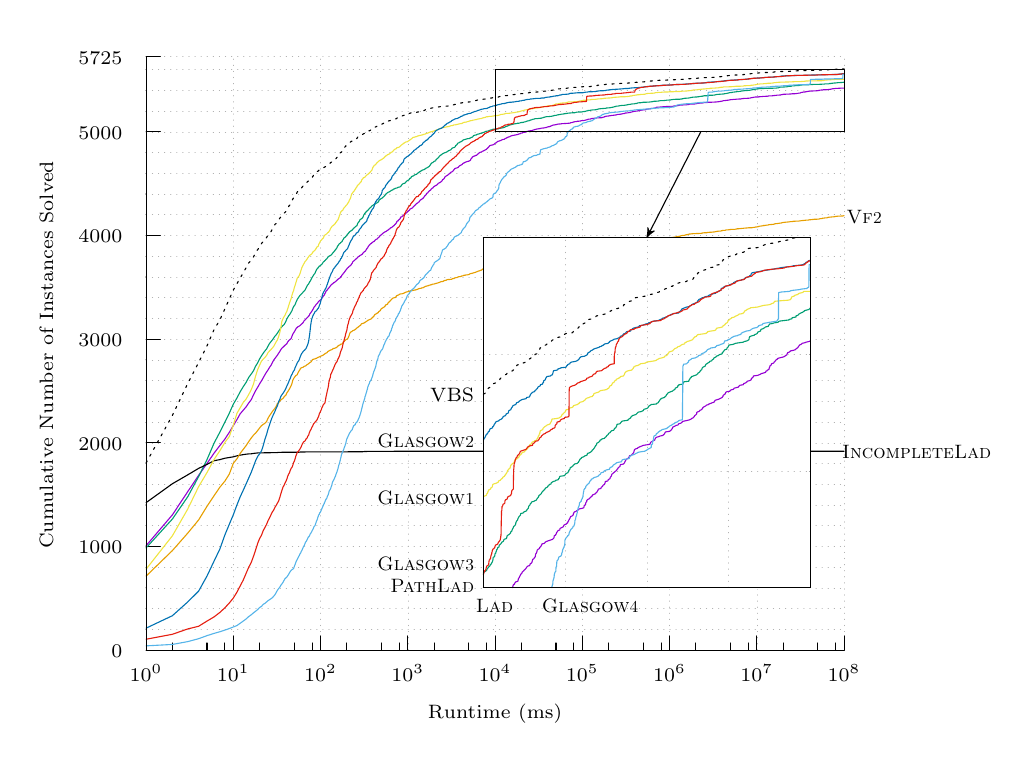
\begin{tikzpicture}[gnuplot]
%% generated with GNUPLOT 5.0p0 (Lua 5.2; terminal rev. 99, script rev. 100)
%% Wed 16 Dec 2015 16:57:53 GMT
\tikzset{every node/.append style={font={\scriptsize}}}
\path (0.000,0.000) rectangle (10.922,8.890);
\gpcolor{color=gp lt color axes}
\gpsetlinetype{gp lt axes}
\gpsetdashtype{gp dt axes}
\gpsetlinewidth{0.50}
\draw[gp path] (1.504,8.521)--(10.368,8.521);
\gpcolor{color=gp lt color border}
\gpsetlinetype{gp lt border}
\gpsetdashtype{gp dt solid}
\gpsetlinewidth{1.00}
\draw[gp path] (1.504,8.521)--(1.684,8.521);
\node[gp node right] at (1.320,8.521) {$5725$};
\gpcolor{color=gp lt color axes}
\gpsetlinetype{gp lt axes}
\gpsetdashtype{gp dt axes}
\gpsetlinewidth{0.50}
\draw[gp path] (1.504,0.985)--(10.368,0.985);
\gpcolor{color=gp lt color border}
\gpsetlinetype{gp lt border}
\gpsetdashtype{gp dt solid}
\gpsetlinewidth{1.00}
\draw[gp path] (1.504,0.985)--(1.684,0.985);
\node[gp node right] at (1.320,0.985) {$0$};
\gpcolor{color=gp lt color axes}
\gpsetlinetype{gp lt axes}
\gpsetdashtype{gp dt axes}
\gpsetlinewidth{0.50}
\draw[gp path] (1.504,1.248)--(10.368,1.248);
\gpcolor{color=gp lt color border}
\gpsetlinetype{gp lt border}
\gpsetdashtype{gp dt solid}
\gpsetlinewidth{1.00}
\draw[gp path] (1.504,1.248)--(1.505,1.248);
\gpcolor{color=gp lt color axes}
\gpsetlinetype{gp lt axes}
\gpsetdashtype{gp dt axes}
\gpsetlinewidth{0.50}
\draw[gp path] (1.504,1.512)--(10.368,1.512);
\gpcolor{color=gp lt color border}
\gpsetlinetype{gp lt border}
\gpsetdashtype{gp dt solid}
\gpsetlinewidth{1.00}
\draw[gp path] (1.504,1.512)--(1.505,1.512);
\gpcolor{color=gp lt color axes}
\gpsetlinetype{gp lt axes}
\gpsetdashtype{gp dt axes}
\gpsetlinewidth{0.50}
\draw[gp path] (1.504,1.775)--(10.368,1.775);
\gpcolor{color=gp lt color border}
\gpsetlinetype{gp lt border}
\gpsetdashtype{gp dt solid}
\gpsetlinewidth{1.00}
\draw[gp path] (1.504,1.775)--(1.505,1.775);
\gpcolor{color=gp lt color axes}
\gpsetlinetype{gp lt axes}
\gpsetdashtype{gp dt axes}
\gpsetlinewidth{0.50}
\draw[gp path] (1.504,2.038)--(10.368,2.038);
\gpcolor{color=gp lt color border}
\gpsetlinetype{gp lt border}
\gpsetdashtype{gp dt solid}
\gpsetlinewidth{1.00}
\draw[gp path] (1.504,2.038)--(1.505,2.038);
\gpcolor{color=gp lt color axes}
\gpsetlinetype{gp lt axes}
\gpsetdashtype{gp dt axes}
\gpsetlinewidth{0.50}
\draw[gp path] (1.504,2.301)--(10.368,2.301);
\gpcolor{color=gp lt color border}
\gpsetlinetype{gp lt border}
\gpsetdashtype{gp dt solid}
\gpsetlinewidth{1.00}
\draw[gp path] (1.504,2.301)--(1.684,2.301);
\node[gp node right] at (1.320,2.301) {$1000$};
\gpcolor{color=gp lt color axes}
\gpsetlinetype{gp lt axes}
\gpsetdashtype{gp dt axes}
\gpsetlinewidth{0.50}
\draw[gp path] (1.504,2.565)--(10.368,2.565);
\gpcolor{color=gp lt color border}
\gpsetlinetype{gp lt border}
\gpsetdashtype{gp dt solid}
\gpsetlinewidth{1.00}
\draw[gp path] (1.504,2.565)--(1.505,2.565);
\gpcolor{color=gp lt color axes}
\gpsetlinetype{gp lt axes}
\gpsetdashtype{gp dt axes}
\gpsetlinewidth{0.50}
\draw[gp path] (1.504,2.828)--(10.368,2.828);
\gpcolor{color=gp lt color border}
\gpsetlinetype{gp lt border}
\gpsetdashtype{gp dt solid}
\gpsetlinewidth{1.00}
\draw[gp path] (1.504,2.828)--(1.505,2.828);
\gpcolor{color=gp lt color axes}
\gpsetlinetype{gp lt axes}
\gpsetdashtype{gp dt axes}
\gpsetlinewidth{0.50}
\draw[gp path] (1.504,3.091)--(10.368,3.091);
\gpcolor{color=gp lt color border}
\gpsetlinetype{gp lt border}
\gpsetdashtype{gp dt solid}
\gpsetlinewidth{1.00}
\draw[gp path] (1.504,3.091)--(1.505,3.091);
\gpcolor{color=gp lt color axes}
\gpsetlinetype{gp lt axes}
\gpsetdashtype{gp dt axes}
\gpsetlinewidth{0.50}
\draw[gp path] (1.504,3.354)--(10.368,3.354);
\gpcolor{color=gp lt color border}
\gpsetlinetype{gp lt border}
\gpsetdashtype{gp dt solid}
\gpsetlinewidth{1.00}
\draw[gp path] (1.504,3.354)--(1.505,3.354);
\gpcolor{color=gp lt color axes}
\gpsetlinetype{gp lt axes}
\gpsetdashtype{gp dt axes}
\gpsetlinewidth{0.50}
\draw[gp path] (1.504,3.618)--(10.368,3.618);
\gpcolor{color=gp lt color border}
\gpsetlinetype{gp lt border}
\gpsetdashtype{gp dt solid}
\gpsetlinewidth{1.00}
\draw[gp path] (1.504,3.618)--(1.684,3.618);
\node[gp node right] at (1.320,3.618) {$2000$};
\gpcolor{color=gp lt color axes}
\gpsetlinetype{gp lt axes}
\gpsetdashtype{gp dt axes}
\gpsetlinewidth{0.50}
\draw[gp path] (1.504,3.881)--(10.368,3.881);
\gpcolor{color=gp lt color border}
\gpsetlinetype{gp lt border}
\gpsetdashtype{gp dt solid}
\gpsetlinewidth{1.00}
\draw[gp path] (1.504,3.881)--(1.505,3.881);
\gpcolor{color=gp lt color axes}
\gpsetlinetype{gp lt axes}
\gpsetdashtype{gp dt axes}
\gpsetlinewidth{0.50}
\draw[gp path] (1.504,4.144)--(10.368,4.144);
\gpcolor{color=gp lt color border}
\gpsetlinetype{gp lt border}
\gpsetdashtype{gp dt solid}
\gpsetlinewidth{1.00}
\draw[gp path] (1.504,4.144)--(1.505,4.144);
\gpcolor{color=gp lt color axes}
\gpsetlinetype{gp lt axes}
\gpsetdashtype{gp dt axes}
\gpsetlinewidth{0.50}
\draw[gp path] (1.504,4.407)--(10.368,4.407);
\gpcolor{color=gp lt color border}
\gpsetlinetype{gp lt border}
\gpsetdashtype{gp dt solid}
\gpsetlinewidth{1.00}
\draw[gp path] (1.504,4.407)--(1.505,4.407);
\gpcolor{color=gp lt color axes}
\gpsetlinetype{gp lt axes}
\gpsetdashtype{gp dt axes}
\gpsetlinewidth{0.50}
\draw[gp path] (1.504,4.671)--(10.368,4.671);
\gpcolor{color=gp lt color border}
\gpsetlinetype{gp lt border}
\gpsetdashtype{gp dt solid}
\gpsetlinewidth{1.00}
\draw[gp path] (1.504,4.671)--(1.505,4.671);
\gpcolor{color=gp lt color axes}
\gpsetlinetype{gp lt axes}
\gpsetdashtype{gp dt axes}
\gpsetlinewidth{0.50}
\draw[gp path] (1.504,4.934)--(10.368,4.934);
\gpcolor{color=gp lt color border}
\gpsetlinetype{gp lt border}
\gpsetdashtype{gp dt solid}
\gpsetlinewidth{1.00}
\draw[gp path] (1.504,4.934)--(1.684,4.934);
\node[gp node right] at (1.320,4.934) {$3000$};
\gpcolor{color=gp lt color axes}
\gpsetlinetype{gp lt axes}
\gpsetdashtype{gp dt axes}
\gpsetlinewidth{0.50}
\draw[gp path] (1.504,5.197)--(10.368,5.197);
\gpcolor{color=gp lt color border}
\gpsetlinetype{gp lt border}
\gpsetdashtype{gp dt solid}
\gpsetlinewidth{1.00}
\draw[gp path] (1.504,5.197)--(1.505,5.197);
\gpcolor{color=gp lt color axes}
\gpsetlinetype{gp lt axes}
\gpsetdashtype{gp dt axes}
\gpsetlinewidth{0.50}
\draw[gp path] (1.504,5.461)--(10.368,5.461);
\gpcolor{color=gp lt color border}
\gpsetlinetype{gp lt border}
\gpsetdashtype{gp dt solid}
\gpsetlinewidth{1.00}
\draw[gp path] (1.504,5.461)--(1.505,5.461);
\gpcolor{color=gp lt color axes}
\gpsetlinetype{gp lt axes}
\gpsetdashtype{gp dt axes}
\gpsetlinewidth{0.50}
\draw[gp path] (1.504,5.724)--(10.368,5.724);
\gpcolor{color=gp lt color border}
\gpsetlinetype{gp lt border}
\gpsetdashtype{gp dt solid}
\gpsetlinewidth{1.00}
\draw[gp path] (1.504,5.724)--(1.505,5.724);
\gpcolor{color=gp lt color axes}
\gpsetlinetype{gp lt axes}
\gpsetdashtype{gp dt axes}
\gpsetlinewidth{0.50}
\draw[gp path] (1.504,5.987)--(10.368,5.987);
\gpcolor{color=gp lt color border}
\gpsetlinetype{gp lt border}
\gpsetdashtype{gp dt solid}
\gpsetlinewidth{1.00}
\draw[gp path] (1.504,5.987)--(1.505,5.987);
\gpcolor{color=gp lt color axes}
\gpsetlinetype{gp lt axes}
\gpsetdashtype{gp dt axes}
\gpsetlinewidth{0.50}
\draw[gp path] (1.504,6.250)--(10.368,6.250);
\gpcolor{color=gp lt color border}
\gpsetlinetype{gp lt border}
\gpsetdashtype{gp dt solid}
\gpsetlinewidth{1.00}
\draw[gp path] (1.504,6.250)--(1.684,6.250);
\node[gp node right] at (1.320,6.250) {$4000$};
\gpcolor{color=gp lt color axes}
\gpsetlinetype{gp lt axes}
\gpsetdashtype{gp dt axes}
\gpsetlinewidth{0.50}
\draw[gp path] (1.504,6.514)--(10.368,6.514);
\gpcolor{color=gp lt color border}
\gpsetlinetype{gp lt border}
\gpsetdashtype{gp dt solid}
\gpsetlinewidth{1.00}
\draw[gp path] (1.504,6.514)--(1.505,6.514);
\gpcolor{color=gp lt color axes}
\gpsetlinetype{gp lt axes}
\gpsetdashtype{gp dt axes}
\gpsetlinewidth{0.50}
\draw[gp path] (1.504,6.777)--(10.368,6.777);
\gpcolor{color=gp lt color border}
\gpsetlinetype{gp lt border}
\gpsetdashtype{gp dt solid}
\gpsetlinewidth{1.00}
\draw[gp path] (1.504,6.777)--(1.505,6.777);
\gpcolor{color=gp lt color axes}
\gpsetlinetype{gp lt axes}
\gpsetdashtype{gp dt axes}
\gpsetlinewidth{0.50}
\draw[gp path] (1.504,7.040)--(10.368,7.040);
\gpcolor{color=gp lt color border}
\gpsetlinetype{gp lt border}
\gpsetdashtype{gp dt solid}
\gpsetlinewidth{1.00}
\draw[gp path] (1.504,7.040)--(1.505,7.040);
\gpcolor{color=gp lt color axes}
\gpsetlinetype{gp lt axes}
\gpsetdashtype{gp dt axes}
\gpsetlinewidth{0.50}
\draw[gp path] (1.504,7.303)--(10.368,7.303);
\gpcolor{color=gp lt color border}
\gpsetlinetype{gp lt border}
\gpsetdashtype{gp dt solid}
\gpsetlinewidth{1.00}
\draw[gp path] (1.504,7.303)--(1.505,7.303);
\gpcolor{color=gp lt color axes}
\gpsetlinetype{gp lt axes}
\gpsetdashtype{gp dt axes}
\gpsetlinewidth{0.50}
\draw[gp path] (1.504,7.567)--(10.368,7.567);
\gpcolor{color=gp lt color border}
\gpsetlinetype{gp lt border}
\gpsetdashtype{gp dt solid}
\gpsetlinewidth{1.00}
\draw[gp path] (1.504,7.567)--(1.684,7.567);
\node[gp node right] at (1.320,7.567) {$5000$};
\gpcolor{color=gp lt color axes}
\gpsetlinetype{gp lt axes}
\gpsetdashtype{gp dt axes}
\gpsetlinewidth{0.50}
\draw[gp path] (1.504,7.830)--(10.368,7.830);
\gpcolor{color=gp lt color border}
\gpsetlinetype{gp lt border}
\gpsetdashtype{gp dt solid}
\gpsetlinewidth{1.00}
\draw[gp path] (1.504,7.830)--(1.505,7.830);
\gpcolor{color=gp lt color axes}
\gpsetlinetype{gp lt axes}
\gpsetdashtype{gp dt axes}
\gpsetlinewidth{0.50}
\draw[gp path] (1.504,8.093)--(10.368,8.093);
\gpcolor{color=gp lt color border}
\gpsetlinetype{gp lt border}
\gpsetdashtype{gp dt solid}
\gpsetlinewidth{1.00}
\draw[gp path] (1.504,8.093)--(1.505,8.093);
\gpcolor{color=gp lt color axes}
\gpsetlinetype{gp lt axes}
\gpsetdashtype{gp dt axes}
\gpsetlinewidth{0.50}
\draw[gp path] (1.504,8.356)--(10.368,8.356);
\gpcolor{color=gp lt color border}
\gpsetlinetype{gp lt border}
\gpsetdashtype{gp dt solid}
\gpsetlinewidth{1.00}
\draw[gp path] (1.504,8.356)--(1.505,8.356);
\gpcolor{color=gp lt color axes}
\gpsetlinetype{gp lt axes}
\gpsetdashtype{gp dt axes}
\gpsetlinewidth{0.50}
\draw[gp path] (1.504,0.985)--(1.504,8.521);
\gpcolor{color=gp lt color border}
\gpsetlinetype{gp lt border}
\gpsetdashtype{gp dt solid}
\gpsetlinewidth{1.00}
\draw[gp path] (1.504,0.985)--(1.504,1.165);
\node[gp node center] at (1.504,0.677) {$10^{0}$};
\draw[gp path] (1.838,0.985)--(1.838,1.075);
\draw[gp path] (2.278,0.985)--(2.278,1.075);
\draw[gp path] (2.505,0.985)--(2.505,1.075);
\gpcolor{color=gp lt color axes}
\gpsetlinetype{gp lt axes}
\gpsetdashtype{gp dt axes}
\gpsetlinewidth{0.50}
\draw[gp path] (2.612,0.985)--(2.612,8.521);
\gpcolor{color=gp lt color border}
\gpsetlinetype{gp lt border}
\gpsetdashtype{gp dt solid}
\gpsetlinewidth{1.00}
\draw[gp path] (2.612,0.985)--(2.612,1.165);
\node[gp node center] at (2.612,0.677) {$10^{1}$};
\draw[gp path] (2.946,0.985)--(2.946,1.075);
\draw[gp path] (3.386,0.985)--(3.386,1.075);
\draw[gp path] (3.613,0.985)--(3.613,1.075);
\gpcolor{color=gp lt color axes}
\gpsetlinetype{gp lt axes}
\gpsetdashtype{gp dt axes}
\gpsetlinewidth{0.50}
\draw[gp path] (3.720,0.985)--(3.720,8.521);
\gpcolor{color=gp lt color border}
\gpsetlinetype{gp lt border}
\gpsetdashtype{gp dt solid}
\gpsetlinewidth{1.00}
\draw[gp path] (3.720,0.985)--(3.720,1.165);
\node[gp node center] at (3.720,0.677) {$10^{2}$};
\draw[gp path] (4.054,0.985)--(4.054,1.075);
\draw[gp path] (4.494,0.985)--(4.494,1.075);
\draw[gp path] (4.721,0.985)--(4.721,1.075);
\gpcolor{color=gp lt color axes}
\gpsetlinetype{gp lt axes}
\gpsetdashtype{gp dt axes}
\gpsetlinewidth{0.50}
\draw[gp path] (4.828,0.985)--(4.828,8.521);
\gpcolor{color=gp lt color border}
\gpsetlinetype{gp lt border}
\gpsetdashtype{gp dt solid}
\gpsetlinewidth{1.00}
\draw[gp path] (4.828,0.985)--(4.828,1.165);
\node[gp node center] at (4.828,0.677) {$10^{3}$};
\draw[gp path] (5.162,0.985)--(5.162,1.075);
\draw[gp path] (5.602,0.985)--(5.602,1.075);
\draw[gp path] (5.829,0.985)--(5.829,1.075);
\gpcolor{color=gp lt color axes}
\gpsetlinetype{gp lt axes}
\gpsetdashtype{gp dt axes}
\gpsetlinewidth{0.50}
\draw[gp path] (5.936,0.985)--(5.936,8.521);
\gpcolor{color=gp lt color border}
\gpsetlinetype{gp lt border}
\gpsetdashtype{gp dt solid}
\gpsetlinewidth{1.00}
\draw[gp path] (5.936,0.985)--(5.936,1.165);
\node[gp node center] at (5.936,0.677) {$10^{4}$};
\draw[gp path] (6.270,0.985)--(6.270,1.075);
\draw[gp path] (6.710,0.985)--(6.710,1.075);
\draw[gp path] (6.937,0.985)--(6.937,1.075);
\gpcolor{color=gp lt color axes}
\gpsetlinetype{gp lt axes}
\gpsetdashtype{gp dt axes}
\gpsetlinewidth{0.50}
\draw[gp path] (7.044,0.985)--(7.044,8.521);
\gpcolor{color=gp lt color border}
\gpsetlinetype{gp lt border}
\gpsetdashtype{gp dt solid}
\gpsetlinewidth{1.00}
\draw[gp path] (7.044,0.985)--(7.044,1.165);
\node[gp node center] at (7.044,0.677) {$10^{5}$};
\draw[gp path] (7.378,0.985)--(7.378,1.075);
\draw[gp path] (7.818,0.985)--(7.818,1.075);
\draw[gp path] (8.045,0.985)--(8.045,1.075);
\gpcolor{color=gp lt color axes}
\gpsetlinetype{gp lt axes}
\gpsetdashtype{gp dt axes}
\gpsetlinewidth{0.50}
\draw[gp path] (8.152,0.985)--(8.152,8.521);
\gpcolor{color=gp lt color border}
\gpsetlinetype{gp lt border}
\gpsetdashtype{gp dt solid}
\gpsetlinewidth{1.00}
\draw[gp path] (8.152,0.985)--(8.152,1.165);
\node[gp node center] at (8.152,0.677) {$10^{6}$};
\draw[gp path] (8.486,0.985)--(8.486,1.075);
\draw[gp path] (8.926,0.985)--(8.926,1.075);
\draw[gp path] (9.153,0.985)--(9.153,1.075);
\gpcolor{color=gp lt color axes}
\gpsetlinetype{gp lt axes}
\gpsetdashtype{gp dt axes}
\gpsetlinewidth{0.50}
\draw[gp path] (9.260,0.985)--(9.260,8.521);
\gpcolor{color=gp lt color border}
\gpsetlinetype{gp lt border}
\gpsetdashtype{gp dt solid}
\gpsetlinewidth{1.00}
\draw[gp path] (9.260,0.985)--(9.260,1.165);
\node[gp node center] at (9.260,0.677) {$10^{7}$};
\draw[gp path] (9.594,0.985)--(9.594,1.075);
\draw[gp path] (10.034,0.985)--(10.034,1.075);
\draw[gp path] (10.261,0.985)--(10.261,1.075);
\gpcolor{color=gp lt color axes}
\gpsetlinetype{gp lt axes}
\gpsetdashtype{gp dt axes}
\gpsetlinewidth{0.50}
\draw[gp path] (10.368,0.985)--(10.368,8.521);
\gpcolor{color=gp lt color border}
\gpsetlinetype{gp lt border}
\gpsetdashtype{gp dt solid}
\gpsetlinewidth{1.00}
\draw[gp path] (10.368,0.985)--(10.368,1.165);
\node[gp node center] at (10.368,0.677) {$10^{8}$};
\draw[gp path] (1.504,8.521)--(1.504,0.985)--(10.368,0.985);
\node[gp node center,rotate=-270] at (0.246,4.753) {Cumulative Number of Instances Solved};
\node[gp node center] at (5.936,0.215) {Runtime (ms)};
\gpcolor{rgb color={0.580,0.000,0.827}}
\draw[gp path] (1.504,2.311)--(1.838,2.703)--(2.033,2.998)--(2.171,3.204)--(2.278,3.356)%
  --(2.366,3.485)--(2.440,3.582)--(2.505,3.666)--(2.561,3.751)--(2.612,3.837)--(2.658,3.913)%
  --(2.700,3.988)--(2.738,4.032)--(2.774,4.074)--(2.807,4.123)--(2.838,4.164)--(2.867,4.224)%
  --(2.895,4.280)--(2.921,4.323)--(2.946,4.367)--(2.969,4.404)--(2.991,4.442)--(3.013,4.482)%
  --(3.033,4.515)--(3.053,4.544)--(3.072,4.576)--(3.090,4.602)--(3.107,4.634)--(3.124,4.667)%
  --(3.141,4.690)--(3.156,4.710)--(3.172,4.731)--(3.187,4.756)--(3.201,4.775)--(3.215,4.801)%
  --(3.228,4.819)--(3.242,4.831)--(3.254,4.843)--(3.267,4.856)--(3.279,4.866)--(3.291,4.876)%
  --(3.303,4.900)--(3.314,4.913)--(3.325,4.925)--(3.336,4.933)--(3.346,4.942)--(3.357,4.973)%
  --(3.367,4.997)--(3.377,5.013)--(3.386,5.027)--(3.396,5.045)--(3.405,5.062)--(3.414,5.076)%
  --(3.423,5.081)--(3.432,5.093)--(3.441,5.095)--(3.450,5.101)--(3.458,5.106)--(3.466,5.113)%
  --(3.474,5.122)--(3.482,5.129)--(3.490,5.135)--(3.498,5.145)--(3.505,5.156)--(3.513,5.172)%
  --(3.520,5.176)--(3.527,5.181)--(3.534,5.192)--(3.541,5.197)--(3.548,5.206)--(3.555,5.212)%
  --(3.562,5.220)--(3.569,5.228)--(3.575,5.233)--(3.582,5.251)--(3.588,5.262)--(3.594,5.268)%
  --(3.600,5.276)--(3.607,5.287)--(3.613,5.295)--(3.619,5.308)--(3.625,5.314)--(3.630,5.326)%
  --(3.636,5.338)--(3.642,5.346)--(3.647,5.351)--(3.653,5.359)--(3.658,5.367)--(3.664,5.374)%
  --(3.669,5.379)--(3.675,5.385)--(3.680,5.392)--(3.685,5.395)--(3.690,5.408)--(3.695,5.413)%
  --(3.700,5.417)--(3.705,5.420)--(3.710,5.426)--(3.715,5.429)--(3.720,5.433)--(3.725,5.436)%
  --(3.730,5.441)--(3.734,5.446)--(3.739,5.462)--(3.743,5.468)--(3.748,5.474)--(3.753,5.478)%
  --(3.757,5.484)--(3.761,5.487)--(3.766,5.493)--(3.770,5.501)--(3.775,5.516)--(3.779,5.518)%
  --(3.783,5.528)--(3.787,5.537)--(3.791,5.546)--(3.796,5.550)--(3.804,5.558)--(3.808,5.563)%
  --(3.812,5.570)--(3.816,5.576)--(3.820,5.578)--(3.824,5.582)--(3.827,5.588)--(3.831,5.595)%
  --(3.835,5.596)--(3.839,5.603)--(3.843,5.608)--(3.846,5.613)--(3.850,5.616)--(3.854,5.622)%
  --(3.857,5.629)--(3.861,5.630)--(3.864,5.633)--(3.868,5.634)--(3.871,5.637)--(3.875,5.638)%
  --(3.878,5.640)--(3.882,5.646)--(3.885,5.650)--(3.892,5.651)--(3.895,5.655)--(3.899,5.658)%
  --(3.905,5.661)--(3.909,5.666)--(3.915,5.669)--(3.918,5.672)--(3.921,5.676)--(3.925,5.680)%
  --(3.928,5.683)--(3.931,5.684)--(3.934,5.690)--(3.940,5.694)--(3.943,5.697)--(3.949,5.701)%
  --(3.952,5.703)--(3.955,5.704)--(3.958,5.707)--(3.961,5.708)--(3.964,5.711)--(3.967,5.712)%
  --(3.970,5.716)--(3.972,5.721)--(3.975,5.726)--(3.978,5.728)--(3.981,5.729)--(3.984,5.732)%
  --(3.987,5.737)--(3.989,5.744)--(3.992,5.749)--(3.995,5.751)--(4.000,5.754)--(4.003,5.761)%
  --(4.006,5.765)--(4.008,5.770)--(4.011,5.772)--(4.013,5.774)--(4.016,5.775)--(4.019,5.778)%
  --(4.021,5.783)--(4.024,5.786)--(4.026,5.791)--(4.029,5.794)--(4.031,5.798)--(4.034,5.800)%
  --(4.036,5.803)--(4.039,5.805)--(4.041,5.812)--(4.044,5.815)--(4.049,5.819)--(4.051,5.823)%
  --(4.054,5.826)--(4.056,5.832)--(4.058,5.834)--(4.061,5.836)--(4.063,5.838)--(4.068,5.841)%
  --(4.070,5.844)--(4.072,5.845)--(4.075,5.846)--(4.077,5.851)--(4.079,5.853)--(4.082,5.857)%
  --(4.084,5.858)--(4.086,5.861)--(4.091,5.862)--(4.093,5.865)--(4.095,5.866)--(4.097,5.867)%
  --(4.099,5.869)--(4.102,5.874)--(4.106,5.875)--(4.108,5.876)--(4.110,5.882)--(4.112,5.887)%
  --(4.114,5.890)--(4.119,5.894)--(4.121,5.899)--(4.123,5.903)--(4.125,5.907)--(4.127,5.912)%
  --(4.129,5.915)--(4.131,5.919)--(4.133,5.920)--(4.135,5.923)--(4.139,5.925)--(4.141,5.928)%
  --(4.145,5.929)--(4.147,5.932)--(4.149,5.934)--(4.155,5.940)--(4.157,5.941)--(4.159,5.944)%
  --(4.161,5.945)--(4.163,5.948)--(4.165,5.949)--(4.169,5.950)--(4.170,5.952)--(4.172,5.954)%
  --(4.174,5.957)--(4.176,5.958)--(4.180,5.962)--(4.183,5.963)--(4.185,5.966)--(4.187,5.967)%
  --(4.189,5.969)--(4.191,5.970)--(4.193,5.973)--(4.194,5.975)--(4.196,5.980)--(4.198,5.982)%
  --(4.200,5.983)--(4.207,5.986)--(4.210,5.988)--(4.212,5.991)--(4.214,5.992)--(4.215,5.994)%
  --(4.219,5.995)--(4.221,5.996)--(4.222,5.998)--(4.224,5.999)--(4.227,6.000)--(4.232,6.002)%
  --(4.234,6.003)--(4.236,6.005)--(4.239,6.007)--(4.241,6.009)--(4.242,6.011)--(4.245,6.012)%
  --(4.250,6.013)--(4.252,6.016)--(4.253,6.019)--(4.255,6.023)--(4.257,6.024)--(4.258,6.025)%
  --(4.260,6.027)--(4.261,6.031)--(4.263,6.032)--(4.264,6.033)--(4.266,6.037)--(4.271,6.038)%
  --(4.272,6.040)--(4.274,6.041)--(4.275,6.044)--(4.277,6.045)--(4.278,6.046)--(4.280,6.048)%
  --(4.283,6.050)--(4.289,6.052)--(4.292,6.056)--(4.293,6.057)--(4.295,6.058)--(4.296,6.065)%
  --(4.297,6.067)--(4.299,6.070)--(4.302,6.074)--(4.303,6.075)--(4.305,6.078)--(4.306,6.081)%
  --(4.307,6.083)--(4.309,6.086)--(4.310,6.088)--(4.312,6.090)--(4.315,6.091)--(4.316,6.092)%
  --(4.317,6.094)--(4.319,6.096)--(4.320,6.099)--(4.321,6.103)--(4.323,6.106)--(4.324,6.107)%
  --(4.326,6.111)--(4.327,6.112)--(4.328,6.115)--(4.331,6.119)--(4.332,6.120)--(4.334,6.121)%
  --(4.335,6.123)--(4.336,6.125)--(4.338,6.128)--(4.339,6.129)--(4.340,6.131)--(4.343,6.132)%
  --(4.346,6.134)--(4.347,6.138)--(4.348,6.140)--(4.351,6.141)--(4.353,6.142)--(4.355,6.144)%
  --(4.359,6.148)--(4.362,6.149)--(4.367,6.150)--(4.369,6.153)--(4.370,6.157)--(4.371,6.158)%
  --(4.372,6.160)--(4.375,6.161)--(4.379,6.162)--(4.381,6.165)--(4.382,6.167)--(4.387,6.169)%
  --(4.388,6.170)--(4.389,6.171)--(4.394,6.173)--(4.397,6.174)--(4.398,6.175)--(4.402,6.177)%
  --(4.404,6.181)--(4.405,6.182)--(4.406,6.183)--(4.407,6.185)--(4.409,6.187)--(4.411,6.188)%
  --(4.412,6.191)--(4.414,6.192)--(4.415,6.195)--(4.417,6.196)--(4.420,6.198)--(4.421,6.199)%
  --(4.423,6.200)--(4.430,6.203)--(4.432,6.204)--(4.437,6.206)--(4.441,6.208)--(4.443,6.211)%
  --(4.444,6.212)--(4.445,6.213)--(4.447,6.215)--(4.448,6.219)--(4.450,6.220)--(4.452,6.223)%
  --(4.453,6.224)--(4.454,6.225)--(4.459,6.228)--(4.460,6.229)--(4.463,6.231)--(4.465,6.232)%
  --(4.466,6.233)--(4.467,6.235)--(4.468,6.236)--(4.469,6.237)--(4.470,6.240)--(4.471,6.242)%
  --(4.472,6.245)--(4.473,6.246)--(4.475,6.249)--(4.481,6.250)--(4.482,6.252)--(4.483,6.254)%
  --(4.485,6.256)--(4.486,6.258)--(4.491,6.260)--(4.492,6.261)--(4.496,6.263)--(4.498,6.265)%
  --(4.499,6.266)--(4.501,6.267)--(4.502,6.269)--(4.503,6.270)--(4.504,6.271)--(4.505,6.273)%
  --(4.507,6.274)--(4.508,6.275)--(4.509,6.277)--(4.511,6.278)--(4.515,6.281)--(4.518,6.282)%
  --(4.519,6.283)--(4.523,6.287)--(4.527,6.289)--(4.529,6.290)--(4.530,6.291)--(4.531,6.294)%
  --(4.534,6.295)--(4.542,6.296)--(4.544,6.299)--(4.547,6.300)--(4.551,6.302)--(4.557,6.304)%
  --(4.558,6.307)--(4.560,6.308)--(4.561,6.310)--(4.563,6.311)--(4.564,6.312)--(4.567,6.314)%
  --(4.569,6.316)--(4.575,6.317)--(4.576,6.319)--(4.577,6.320)--(4.578,6.321)--(4.580,6.324)%
  --(4.581,6.325)--(4.582,6.327)--(4.586,6.328)--(4.587,6.329)--(4.590,6.331)--(4.592,6.332)%
  --(4.593,6.335)--(4.599,6.336)--(4.600,6.337)--(4.603,6.339)--(4.604,6.344)--(4.606,6.345)%
  --(4.606,6.346)--(4.609,6.348)--(4.611,6.349)--(4.620,6.350)--(4.621,6.352)--(4.623,6.353)%
  --(4.624,6.354)--(4.626,6.356)--(4.627,6.357)--(4.628,6.360)--(4.635,6.361)--(4.635,6.362)%
  --(4.636,6.365)--(4.637,6.366)--(4.639,6.367)--(4.641,6.369)--(4.642,6.370)--(4.644,6.371)%
  --(4.648,6.373)--(4.649,6.374)--(4.650,6.375)--(4.653,6.377)--(4.656,6.378)--(4.657,6.382)%
  --(4.658,6.385)--(4.658,6.386)--(4.660,6.387)--(4.661,6.389)--(4.663,6.390)--(4.664,6.391)%
  --(4.669,6.392)--(4.669,6.394)--(4.670,6.395)--(4.671,6.396)--(4.671,6.398)--(4.675,6.400)%
  --(4.677,6.402)--(4.677,6.404)--(4.678,6.406)--(4.679,6.407)--(4.679,6.408)--(4.682,6.410)%
  --(4.684,6.411)--(4.684,6.414)--(4.685,6.415)--(4.686,6.418)--(4.686,6.421)--(4.688,6.423)%
  --(4.690,6.424)--(4.691,6.428)--(4.691,6.432)--(4.693,6.433)--(4.693,6.435)--(4.704,6.436)%
  --(4.706,6.437)--(4.707,6.439)--(4.708,6.440)--(4.709,6.444)--(4.710,6.446)--(4.711,6.449)%
  --(4.713,6.450)--(4.719,6.452)--(4.720,6.453)--(4.721,6.454)--(4.722,6.456)--(4.723,6.457)%
  --(4.724,6.458)--(4.726,6.461)--(4.727,6.462)--(4.728,6.465)--(4.729,6.468)--(4.732,6.469)%
  --(4.733,6.470)--(4.733,6.471)--(4.734,6.474)--(4.735,6.477)--(4.737,6.481)--(4.738,6.483)%
  --(4.738,6.485)--(4.743,6.486)--(4.745,6.487)--(4.753,6.489)--(4.754,6.491)--(4.754,6.493)%
  --(4.757,6.496)--(4.762,6.498)--(4.763,6.500)--(4.764,6.502)--(4.766,6.503)--(4.767,6.504)%
  --(4.768,6.506)--(4.769,6.507)--(4.770,6.508)--(4.772,6.511)--(4.783,6.512)--(4.783,6.514)%
  --(4.784,6.515)--(4.789,6.516)--(4.789,6.518)--(4.790,6.519)--(4.792,6.520)--(4.794,6.521)%
  --(4.794,6.524)--(4.795,6.525)--(4.796,6.527)--(4.797,6.528)--(4.798,6.529)--(4.800,6.531)%
  --(4.801,6.532)--(4.804,6.533)--(4.807,6.536)--(4.809,6.537)--(4.810,6.539)--(4.812,6.540)%
  --(4.814,6.541)--(4.816,6.543)--(4.819,6.545)--(4.820,6.547)--(4.821,6.548)--(4.821,6.550)%
  --(4.822,6.552)--(4.823,6.553)--(4.823,6.554)--(4.826,6.556)--(4.827,6.557)--(4.829,6.558)%
  --(4.832,6.560)--(4.833,6.562)--(4.837,6.564)--(4.838,6.566)--(4.840,6.568)--(4.843,6.569)%
  --(4.848,6.570)--(4.849,6.572)--(4.850,6.573)--(4.851,6.574)--(4.851,6.577)--(4.851,6.578)%
  --(4.852,6.579)--(4.853,6.583)--(4.855,6.586)--(4.856,6.587)--(4.861,6.589)--(4.865,6.590)%
  --(4.868,6.591)--(4.869,6.593)--(4.869,6.594)--(4.873,6.595)--(4.876,6.597)--(4.882,6.598)%
  --(4.883,6.599)--(4.886,6.600)--(4.886,6.602)--(4.889,6.604)--(4.891,6.606)--(4.893,6.608)%
  --(4.893,6.610)--(4.894,6.611)--(4.896,6.612)--(4.897,6.614)--(4.897,6.615)--(4.901,6.616)%
  --(4.902,6.619)--(4.904,6.620)--(4.906,6.623)--(4.907,6.624)--(4.909,6.625)--(4.911,6.627)%
  --(4.913,6.629)--(4.913,6.631)--(4.914,6.632)--(4.915,6.633)--(4.917,6.635)--(4.921,6.636)%
  --(4.921,6.637)--(4.925,6.640)--(4.926,6.641)--(4.926,6.643)--(4.927,6.644)--(4.927,6.645)%
  --(4.928,6.647)--(4.931,6.648)--(4.932,6.649)--(4.933,6.650)--(4.938,6.652)--(4.939,6.653)%
  --(4.940,6.656)--(4.941,6.657)--(4.943,6.658)--(4.944,6.660)--(4.950,6.661)--(4.950,6.662)%
  --(4.954,6.665)--(4.955,6.666)--(4.955,6.668)--(4.958,6.669)--(4.958,6.670)--(4.960,6.672)%
  --(4.963,6.673)--(4.964,6.674)--(4.966,6.676)--(4.971,6.677)--(4.972,6.678)--(4.973,6.679)%
  --(4.973,6.681)--(4.974,6.682)--(4.976,6.685)--(4.976,6.686)--(4.977,6.689)--(4.979,6.690)%
  --(4.980,6.691)--(4.981,6.693)--(4.982,6.694)--(4.983,6.695)--(4.984,6.697)--(4.986,6.698)%
  --(4.986,6.699)--(4.987,6.701)--(4.989,6.702)--(4.991,6.703)--(4.994,6.704)--(4.996,6.706)%
  --(4.998,6.707)--(5.000,6.708)--(5.004,6.710)--(5.005,6.711)--(5.005,6.712)--(5.007,6.714)%
  --(5.011,6.716)--(5.012,6.718)--(5.016,6.719)--(5.019,6.720)--(5.019,6.722)--(5.020,6.723)%
  --(5.022,6.724)--(5.023,6.726)--(5.025,6.728)--(5.026,6.729)--(5.026,6.731)--(5.030,6.735)%
  --(5.031,6.736)--(5.032,6.737)--(5.034,6.740)--(5.036,6.743)--(5.037,6.744)--(5.039,6.745)%
  --(5.039,6.747)--(5.040,6.748)--(5.040,6.749)--(5.041,6.751)--(5.043,6.754)--(5.045,6.756)%
  --(5.048,6.757)--(5.049,6.758)--(5.051,6.760)--(5.053,6.761)--(5.054,6.762)--(5.054,6.764)%
  --(5.057,6.765)--(5.058,6.768)--(5.059,6.769)--(5.059,6.770)--(5.060,6.772)--(5.060,6.773)%
  --(5.061,6.774)--(5.064,6.776)--(5.064,6.777)--(5.065,6.778)--(5.065,6.779)--(5.066,6.781)%
  --(5.067,6.783)--(5.067,6.785)--(5.069,6.786)--(5.069,6.787)--(5.071,6.789)--(5.078,6.790)%
  --(5.082,6.791)--(5.082,6.794)--(5.083,6.797)--(5.084,6.798)--(5.085,6.799)--(5.087,6.801)%
  --(5.087,6.802)--(5.088,6.803)--(5.088,6.805)--(5.088,6.806)--(5.090,6.807)--(5.092,6.808)%
  --(5.093,6.811)--(5.097,6.812)--(5.098,6.814)--(5.100,6.815)--(5.102,6.816)--(5.103,6.818)%
  --(5.103,6.819)--(5.104,6.820)--(5.106,6.822)--(5.106,6.823)--(5.111,6.824)--(5.115,6.826)%
  --(5.116,6.827)--(5.117,6.828)--(5.117,6.830)--(5.119,6.831)--(5.121,6.832)--(5.121,6.836)%
  --(5.122,6.837)--(5.122,6.839)--(5.125,6.840)--(5.130,6.843)--(5.131,6.844)--(5.131,6.845)%
  --(5.132,6.847)--(5.134,6.848)--(5.134,6.849)--(5.136,6.852)--(5.146,6.853)--(5.146,6.855)%
  --(5.147,6.857)--(5.147,6.858)--(5.148,6.860)--(5.149,6.861)--(5.149,6.862)--(5.154,6.864)%
  --(5.155,6.865)--(5.156,6.866)--(5.156,6.870)--(5.163,6.873)--(5.165,6.874)--(5.166,6.876)%
  --(5.168,6.877)--(5.171,6.880)--(5.174,6.881)--(5.177,6.882)--(5.178,6.883)--(5.181,6.885)%
  --(5.186,6.886)--(5.187,6.887)--(5.189,6.889)--(5.189,6.890)--(5.192,6.891)--(5.194,6.893)%
  --(5.197,6.894)--(5.199,6.895)--(5.201,6.897)--(5.203,6.898)--(5.204,6.899)--(5.206,6.901)%
  --(5.206,6.902)--(5.208,6.903)--(5.210,6.906)--(5.210,6.907)--(5.211,6.908)--(5.211,6.910)%
  --(5.214,6.912)--(5.217,6.915)--(5.225,6.916)--(5.226,6.918)--(5.226,6.919)--(5.227,6.920)%
  --(5.232,6.922)--(5.236,6.923)--(5.239,6.924)--(5.239,6.926)--(5.240,6.927)--(5.241,6.928)%
  --(5.245,6.930)--(5.246,6.931)--(5.250,6.932)--(5.251,6.935)--(5.251,6.936)--(5.255,6.937)%
  --(5.255,6.939)--(5.259,6.941)--(5.260,6.943)--(5.261,6.944)--(5.262,6.945)--(5.263,6.947)%
  --(5.263,6.948)--(5.264,6.949)--(5.265,6.952)--(5.265,6.953)--(5.267,6.955)--(5.268,6.956)%
  --(5.268,6.957)--(5.269,6.959)--(5.270,6.960)--(5.275,6.962)--(5.277,6.964)--(5.278,6.965)%
  --(5.281,6.966)--(5.282,6.968)--(5.283,6.969)--(5.284,6.970)--(5.286,6.972)--(5.289,6.973)%
  --(5.290,6.974)--(5.291,6.976)--(5.292,6.977)--(5.292,6.978)--(5.293,6.981)--(5.294,6.982)%
  --(5.294,6.984)--(5.294,6.985)--(5.294,6.986)--(5.296,6.987)--(5.297,6.989)--(5.298,6.990)%
  --(5.299,6.993)--(5.300,6.994)--(5.301,6.995)--(5.302,6.997)--(5.305,6.998)--(5.306,6.999)%
  --(5.308,7.001)--(5.310,7.002)--(5.312,7.003)--(5.312,7.005)--(5.314,7.006)--(5.315,7.007)%
  --(5.318,7.009)--(5.323,7.010)--(5.326,7.011)--(5.327,7.012)--(5.329,7.014)--(5.331,7.015)%
  --(5.332,7.016)--(5.333,7.018)--(5.338,7.019)--(5.338,7.020)--(5.339,7.022)--(5.340,7.023)%
  --(5.341,7.024)--(5.341,7.026)--(5.347,7.027)--(5.347,7.028)--(5.350,7.030)--(5.352,7.031)%
  --(5.352,7.032)--(5.353,7.034)--(5.353,7.035)--(5.354,7.036)--(5.355,7.037)--(5.361,7.039)%
  --(5.361,7.040)--(5.363,7.041)--(5.365,7.043)--(5.366,7.044)--(5.368,7.047)--(5.369,7.049)%
  --(5.372,7.052)--(5.374,7.053)--(5.378,7.055)--(5.379,7.056)--(5.384,7.057)--(5.385,7.059)%
  --(5.389,7.060)--(5.392,7.061)--(5.392,7.063)--(5.393,7.064)--(5.396,7.065)--(5.399,7.066)%
  --(5.400,7.068)--(5.400,7.069)--(5.402,7.070)--(5.403,7.072)--(5.404,7.073)--(5.405,7.074)%
  --(5.405,7.076)--(5.409,7.078)--(5.409,7.080)--(5.410,7.081)--(5.411,7.082)--(5.412,7.084)%
  --(5.413,7.085)--(5.414,7.086)--(5.416,7.088)--(5.416,7.089)--(5.417,7.090)--(5.418,7.091)%
  --(5.419,7.093)--(5.420,7.094)--(5.421,7.095)--(5.422,7.097)--(5.424,7.098)--(5.424,7.099)%
  --(5.426,7.101)--(5.432,7.102)--(5.435,7.103)--(5.436,7.105)--(5.439,7.106)--(5.450,7.107)%
  --(5.451,7.109)--(5.451,7.110)--(5.454,7.111)--(5.460,7.113)--(5.464,7.114)--(5.464,7.115)%
  --(5.468,7.116)--(5.470,7.118)--(5.471,7.119)--(5.471,7.120)--(5.471,7.122)--(5.473,7.123)%
  --(5.474,7.124)--(5.475,7.126)--(5.478,7.127)--(5.478,7.128)--(5.478,7.130)--(5.478,7.131)%
  --(5.481,7.132)--(5.482,7.134)--(5.484,7.135)--(5.485,7.136)--(5.489,7.138)--(5.491,7.139)%
  --(5.496,7.140)--(5.497,7.141)--(5.497,7.143)--(5.497,7.144)--(5.505,7.145)--(5.506,7.147)%
  --(5.511,7.148)--(5.512,7.149)--(5.512,7.151)--(5.517,7.152)--(5.518,7.153)--(5.519,7.155)%
  --(5.521,7.157)--(5.522,7.159)--(5.523,7.160)--(5.524,7.161)--(5.525,7.163)--(5.528,7.164)%
  --(5.528,7.166)--(5.533,7.168)--(5.533,7.169)--(5.541,7.170)--(5.543,7.172)--(5.544,7.173)%
  --(5.544,7.174)--(5.545,7.176)--(5.548,7.177)--(5.551,7.178)--(5.558,7.180)--(5.560,7.181)%
  --(5.561,7.182)--(5.565,7.184)--(5.568,7.185)--(5.572,7.186)--(5.577,7.188)--(5.581,7.189)%
  --(5.584,7.190)--(5.592,7.192)--(5.596,7.193)--(5.601,7.194)--(5.602,7.195)--(5.607,7.197)%
  --(5.610,7.198)--(5.613,7.199)--(5.614,7.201)--(5.618,7.202)--(5.619,7.203)--(5.621,7.205)%
  --(5.623,7.206)--(5.623,7.207)--(5.624,7.209)--(5.624,7.210)--(5.626,7.211)--(5.626,7.214)%
  --(5.626,7.215)--(5.627,7.217)--(5.627,7.218)--(5.627,7.219)--(5.628,7.220)--(5.629,7.222)%
  --(5.629,7.223)--(5.629,7.224)--(5.632,7.226)--(5.633,7.227)--(5.634,7.228)--(5.635,7.230)%
  --(5.636,7.231)--(5.638,7.232)--(5.639,7.234)--(5.639,7.235)--(5.642,7.236)--(5.643,7.238)%
  --(5.643,7.239)--(5.644,7.240)--(5.644,7.242)--(5.645,7.243)--(5.646,7.244)--(5.647,7.245)%
  --(5.647,7.247)--(5.651,7.248)--(5.653,7.249)--(5.655,7.251)--(5.656,7.252)--(5.657,7.253)%
  --(5.662,7.255)--(5.665,7.256)--(5.666,7.257)--(5.667,7.259)--(5.671,7.260)--(5.680,7.261)%
  --(5.685,7.263)--(5.686,7.264)--(5.687,7.267)--(5.692,7.268)--(5.694,7.269)--(5.703,7.270)%
  --(5.704,7.272)--(5.707,7.273)--(5.707,7.274)--(5.708,7.276)--(5.708,7.277)--(5.710,7.278)%
  --(5.710,7.280)--(5.714,7.281)--(5.715,7.282)--(5.716,7.284)--(5.719,7.285)--(5.720,7.286)%
  --(5.721,7.288)--(5.721,7.289)--(5.722,7.290)--(5.722,7.292)--(5.728,7.293)--(5.729,7.294)%
  --(5.731,7.295)--(5.732,7.297)--(5.733,7.298)--(5.734,7.299)--(5.735,7.301)--(5.735,7.302)%
  --(5.737,7.303)--(5.738,7.305)--(5.738,7.306)--(5.748,7.307)--(5.752,7.309)--(5.759,7.310)%
  --(5.761,7.311)--(5.763,7.313)--(5.768,7.314)--(5.770,7.315)--(5.770,7.317)--(5.771,7.318)%
  --(5.774,7.319)--(5.777,7.321)--(5.779,7.322)--(5.783,7.323)--(5.787,7.324)--(5.790,7.326)%
  --(5.790,7.327)--(5.799,7.328)--(5.800,7.330)--(5.802,7.331)--(5.803,7.332)--(5.805,7.334)%
  --(5.808,7.335)--(5.810,7.336)--(5.811,7.338)--(5.814,7.339)--(5.815,7.340)--(5.818,7.342)%
  --(5.824,7.343)--(5.825,7.344)--(5.826,7.346)--(5.826,7.347)--(5.828,7.348)--(5.828,7.349)%
  --(5.829,7.351)--(5.829,7.352)--(5.836,7.353)--(5.838,7.355)--(5.838,7.356)--(5.839,7.357)%
  --(5.839,7.359)--(5.841,7.360)--(5.841,7.361)--(5.844,7.363)--(5.845,7.364)--(5.846,7.365)%
  --(5.850,7.367)--(5.850,7.368)--(5.850,7.369)--(5.852,7.371)--(5.852,7.372)--(5.855,7.373)%
  --(5.856,7.374)--(5.856,7.376)--(5.857,7.377)--(5.858,7.378)--(5.860,7.380)--(5.862,7.381)%
  --(5.862,7.382)--(5.863,7.384)--(5.863,7.385)--(5.864,7.386)--(5.866,7.388)--(5.867,7.389)%
  --(5.868,7.390)--(5.869,7.392)--(5.874,7.393)--(5.875,7.394)--(5.884,7.396)--(5.887,7.397)%
  --(5.892,7.398)--(5.896,7.399)--(5.905,7.401)--(5.905,7.402)--(5.912,7.403)--(5.916,7.405)%
  --(5.919,7.406)--(5.920,7.407)--(5.924,7.409)--(5.925,7.410)--(5.927,7.411)--(5.928,7.413)%
  --(5.929,7.414)--(5.931,7.415)--(5.932,7.417)--(5.933,7.418)--(5.933,7.419)--(5.936,7.421)%
  --(5.937,7.422)--(5.937,7.423)--(5.940,7.424)--(5.942,7.426)--(5.952,7.428)--(5.952,7.430)%
  --(5.953,7.431)--(5.954,7.432)--(5.954,7.434)--(5.958,7.435)--(5.960,7.436)--(5.961,7.438)%
  --(5.962,7.439)--(5.966,7.440)--(5.966,7.442)--(5.968,7.443)--(5.968,7.444)--(5.970,7.446)%
  --(5.974,7.447)--(5.979,7.448)--(5.988,7.450)--(5.991,7.451)--(5.994,7.452)--(5.995,7.453)%
  --(5.996,7.455)--(6.004,7.456)--(6.009,7.457)--(6.012,7.459)--(6.013,7.460)--(6.016,7.461)%
  --(6.017,7.463)--(6.020,7.464)--(6.021,7.465)--(6.025,7.467)--(6.027,7.468)--(6.036,7.469)%
  --(6.038,7.471)--(6.050,7.472)--(6.054,7.473)--(6.057,7.475)--(6.058,7.476)--(6.059,7.477)%
  --(6.059,7.478)--(6.061,7.480)--(6.065,7.481)--(6.066,7.482)--(6.074,7.484)--(6.074,7.485)%
  --(6.078,7.486)--(6.079,7.488)--(6.081,7.489)--(6.085,7.490)--(6.088,7.492)--(6.089,7.493)%
  --(6.089,7.494)--(6.091,7.496)--(6.092,7.497)--(6.099,7.498)--(6.101,7.500)--(6.105,7.501)%
  --(6.111,7.502)--(6.118,7.503)--(6.120,7.505)--(6.123,7.506)--(6.125,7.507)--(6.128,7.509)%
  --(6.130,7.510)--(6.131,7.511)--(6.134,7.513)--(6.135,7.514)--(6.141,7.515)--(6.146,7.517)%
  --(6.146,7.518)--(6.152,7.519)--(6.159,7.521)--(6.168,7.522)--(6.175,7.523)--(6.181,7.525)%
  --(6.182,7.526)--(6.189,7.527)--(6.203,7.528)--(6.204,7.530)--(6.209,7.531)--(6.219,7.532)%
  --(6.222,7.534)--(6.223,7.535)--(6.231,7.536)--(6.238,7.538)--(6.238,7.539)--(6.240,7.540)%
  --(6.250,7.542)--(6.254,7.543)--(6.254,7.544)--(6.258,7.546)--(6.260,7.547)--(6.260,7.548)%
  --(6.262,7.550)--(6.268,7.551)--(6.281,7.552)--(6.281,7.553)--(6.282,7.555)--(6.288,7.556)%
  --(6.288,7.557)--(6.291,7.559)--(6.301,7.560)--(6.317,7.561)--(6.318,7.563)--(6.326,7.564)%
  --(6.330,7.565)--(6.333,7.567)--(6.334,7.568)--(6.335,7.569)--(6.336,7.571)--(6.340,7.572)%
  --(6.343,7.573)--(6.357,7.575)--(6.358,7.576)--(6.361,7.577)--(6.370,7.579)--(6.374,7.580)%
  --(6.402,7.581)--(6.405,7.582)--(6.407,7.584)--(6.408,7.585)--(6.410,7.586)--(6.412,7.588)%
  --(6.422,7.589)--(6.423,7.590)--(6.426,7.592)--(6.432,7.593)--(6.436,7.594)--(6.438,7.596)%
  --(6.445,7.597)--(6.448,7.598)--(6.459,7.600)--(6.461,7.601)--(6.464,7.602)--(6.472,7.604)%
  --(6.484,7.605)--(6.488,7.606)--(6.500,7.607)--(6.504,7.609)--(6.514,7.610)--(6.518,7.611)%
  --(6.521,7.613)--(6.529,7.614)--(6.539,7.615)--(6.563,7.617)--(6.565,7.618)--(6.570,7.619)%
  --(6.571,7.621)--(6.585,7.622)--(6.590,7.623)--(6.595,7.625)--(6.596,7.626)--(6.599,7.627)%
  --(6.602,7.629)--(6.604,7.630)--(6.610,7.631)--(6.624,7.632)--(6.625,7.634)--(6.633,7.635)%
  --(6.639,7.636)--(6.640,7.638)--(6.640,7.639)--(6.643,7.640)--(6.644,7.642)--(6.645,7.643)%
  --(6.654,7.644)--(6.656,7.646)--(6.660,7.647)--(6.663,7.648)--(6.664,7.650)--(6.664,7.651)%
  --(6.670,7.652)--(6.680,7.654)--(6.695,7.655)--(6.698,7.656)--(6.699,7.657)--(6.710,7.659)%
  --(6.713,7.660)--(6.723,7.661)--(6.724,7.663)--(6.729,7.664)--(6.730,7.665)--(6.764,7.667)%
  --(6.768,7.668)--(6.775,7.669)--(6.786,7.671)--(6.809,7.672)--(6.832,7.673)--(6.853,7.675)%
  --(6.876,7.676)--(6.882,7.677)--(6.891,7.679)--(6.894,7.680)--(6.894,7.681)--(6.896,7.682)%
  --(6.897,7.684)--(6.913,7.685)--(6.914,7.686)--(6.923,7.688)--(6.926,7.689)--(6.927,7.690)%
  --(6.931,7.692)--(6.943,7.693)--(6.944,7.694)--(6.947,7.696)--(6.973,7.697)--(6.973,7.698)%
  --(6.974,7.700)--(6.980,7.701)--(6.997,7.702)--(7.015,7.704)--(7.023,7.705)--(7.025,7.706)%
  --(7.028,7.708)--(7.037,7.709)--(7.061,7.710)--(7.061,7.711)--(7.079,7.713)--(7.080,7.714)%
  --(7.081,7.715)--(7.089,7.717)--(7.091,7.718)--(7.095,7.719)--(7.103,7.721)--(7.104,7.722)%
  --(7.110,7.723)--(7.112,7.725)--(7.115,7.726)--(7.119,7.727)--(7.139,7.729)--(7.149,7.730)%
  --(7.154,7.731)--(7.155,7.733)--(7.157,7.734)--(7.163,7.735)--(7.164,7.736)--(7.172,7.738)%
  --(7.193,7.739)--(7.201,7.740)--(7.218,7.742)--(7.226,7.743)--(7.234,7.744)--(7.272,7.746)%
  --(7.298,7.747)--(7.298,7.748)--(7.302,7.750)--(7.303,7.751)--(7.304,7.752)--(7.320,7.754)%
  --(7.321,7.755)--(7.322,7.756)--(7.323,7.758)--(7.327,7.759)--(7.333,7.760)--(7.337,7.761)%
  --(7.338,7.763)--(7.341,7.764)--(7.346,7.765)--(7.365,7.767)--(7.376,7.768)--(7.381,7.769)%
  --(7.389,7.771)--(7.399,7.772)--(7.408,7.773)--(7.415,7.775)--(7.416,7.776)--(7.436,7.777)%
  --(7.453,7.779)--(7.457,7.780)--(7.470,7.781)--(7.476,7.783)--(7.478,7.784)--(7.486,7.785)%
  --(7.491,7.786)--(7.491,7.788)--(7.496,7.789)--(7.528,7.790)--(7.532,7.792)--(7.533,7.793)%
  --(7.545,7.794)--(7.553,7.796)--(7.556,7.797)--(7.562,7.798)--(7.579,7.800)--(7.581,7.801)%
  --(7.584,7.802)--(7.587,7.804)--(7.588,7.805)--(7.590,7.806)--(7.623,7.808)--(7.627,7.809)%
  --(7.628,7.810)--(7.639,7.811)--(7.654,7.813)--(7.655,7.814)--(7.655,7.815)--(7.662,7.817)%
  --(7.670,7.818)--(7.672,7.819)--(7.676,7.821)--(7.677,7.822)--(7.683,7.823)--(7.695,7.825)%
  --(7.699,7.826)--(7.714,7.827)--(7.719,7.829)--(7.731,7.830)--(7.741,7.831)--(7.747,7.833)%
  --(7.748,7.834)--(7.761,7.835)--(7.762,7.837)--(7.765,7.838)--(7.780,7.839)--(7.789,7.840)%
  --(7.790,7.842)--(7.791,7.843)--(7.796,7.844)--(7.836,7.846)--(7.843,7.847)--(7.851,7.848)%
  --(7.852,7.850)--(7.856,7.851)--(7.861,7.852)--(7.864,7.854)--(7.868,7.855)--(7.874,7.856)%
  --(7.887,7.858)--(7.901,7.859)--(7.909,7.860)--(7.912,7.862)--(7.914,7.863)--(7.915,7.864)%
  --(7.943,7.865)--(7.949,7.867)--(7.954,7.868)--(7.962,7.869)--(7.971,7.871)--(7.976,7.872)%
  --(7.978,7.873)--(7.979,7.875)--(7.983,7.876)--(7.983,7.877)--(7.987,7.879)--(8.002,7.880)%
  --(8.027,7.881)--(8.032,7.883)--(8.049,7.884)--(8.064,7.885)--(8.086,7.887)--(8.101,7.888)%
  --(8.157,7.889)--(8.196,7.890)--(8.197,7.892)--(8.201,7.893)--(8.203,7.894)--(8.213,7.896)%
  --(8.229,7.897)--(8.239,7.898)--(8.260,7.900)--(8.261,7.901)--(8.265,7.902)--(8.269,7.904)%
  --(8.274,7.905)--(8.286,7.906)--(8.315,7.908)--(8.332,7.909)--(8.370,7.910)--(8.376,7.912)%
  --(8.387,7.913)--(8.392,7.914)--(8.395,7.915)--(8.403,7.917)--(8.405,7.918)--(8.461,7.919)%
  --(8.470,7.921)--(8.480,7.922)--(8.489,7.923)--(8.491,7.925)--(8.499,7.926)--(8.501,7.927)%
  --(8.502,7.929)--(8.517,7.930)--(8.536,7.931)--(8.546,7.933)--(8.575,7.934)--(8.581,7.935)%
  --(8.584,7.937)--(8.614,7.938)--(8.622,7.939)--(8.634,7.940)--(8.634,7.942)--(8.672,7.943)%
  --(8.710,7.944)--(8.735,7.946)--(8.754,7.947)--(8.759,7.948)--(8.776,7.950)--(8.785,7.951)%
  --(8.792,7.952)--(8.800,7.954)--(8.801,7.955)--(8.813,7.956)--(8.823,7.958)--(8.828,7.959)%
  --(8.829,7.960)--(8.830,7.962)--(8.834,7.963)--(8.856,7.964)--(8.868,7.966)--(8.871,7.967)%
  --(8.892,7.968)--(8.897,7.969)--(8.909,7.971)--(8.910,7.972)--(8.915,7.973)--(8.925,7.975)%
  --(8.942,7.976)--(8.954,7.977)--(8.960,7.979)--(8.993,7.980)--(8.993,7.981)--(9.024,7.983)%
  --(9.036,7.984)--(9.065,7.985)--(9.067,7.987)--(9.075,7.988)--(9.076,7.989)--(9.097,7.991)%
  --(9.124,7.992)--(9.142,7.993)--(9.158,7.994)--(9.175,7.996)--(9.177,7.997)--(9.186,7.998)%
  --(9.187,8.000)--(9.192,8.001)--(9.204,8.002)--(9.213,8.004)--(9.217,8.005)--(9.222,8.006)%
  --(9.224,8.008)--(9.242,8.009)--(9.283,8.010)--(9.283,8.012)--(9.292,8.013)--(9.325,8.014)%
  --(9.333,8.016)--(9.336,8.017)--(9.364,8.018)--(9.397,8.019)--(9.398,8.021)--(9.409,8.022)%
  --(9.414,8.023)--(9.463,8.025)--(9.464,8.026)--(9.467,8.027)--(9.492,8.029)--(9.501,8.030)%
  --(9.512,8.031)--(9.514,8.033)--(9.545,8.034)--(9.564,8.035)--(9.569,8.037)--(9.570,8.038)%
  --(9.572,8.039)--(9.587,8.041)--(9.593,8.042)--(9.597,8.043)--(9.598,8.044)--(9.656,8.046)%
  --(9.675,8.047)--(9.694,8.048)--(9.704,8.050)--(9.735,8.051)--(9.760,8.052)--(9.766,8.054)%
  --(9.768,8.055)--(9.784,8.056)--(9.788,8.058)--(9.809,8.059)--(9.811,8.060)--(9.811,8.062)%
  --(9.814,8.063)--(9.817,8.064)--(9.821,8.066)--(9.821,8.067)--(9.833,8.068)--(9.840,8.069)%
  --(9.842,8.071)--(9.844,8.072)--(9.874,8.073)--(9.878,8.075)--(9.881,8.076)--(9.893,8.077)%
  --(9.895,8.079)--(9.905,8.080)--(9.907,8.081)--(9.927,8.083)--(9.927,8.084)--(9.951,8.085)%
  --(9.989,8.087)--(10.012,8.088)--(10.027,8.089)--(10.033,8.091)--(10.052,8.092)--(10.052,8.093)%
  --(10.057,8.095)--(10.061,8.096)--(10.063,8.097)--(10.086,8.098)--(10.096,8.100)--(10.103,8.101)%
  --(10.144,8.102)--(10.167,8.104)--(10.175,8.105)--(10.180,8.106)--(10.195,8.108)--(10.204,8.109)%
  --(10.207,8.110)--(10.212,8.112)--(10.221,8.113)--(10.222,8.114)--(10.244,8.116)--(10.254,8.117)%
  --(10.257,8.118)--(10.298,8.120)--(10.313,8.121)--(10.352,8.122)--(10.368,8.123);
\gpcolor{rgb color={0.000,0.620,0.451}}
\draw[gp path] (1.504,2.283)--(1.838,2.650)--(2.033,2.933)--(2.171,3.189)--(2.278,3.406)%
  --(2.366,3.611)--(2.440,3.752)--(2.505,3.881)--(2.561,3.995)--(2.612,4.109)--(2.658,4.188)%
  --(2.700,4.268)--(2.738,4.331)--(2.774,4.385)--(2.807,4.448)--(2.838,4.490)--(2.867,4.531)%
  --(2.895,4.592)--(2.921,4.633)--(2.946,4.684)--(2.969,4.722)--(2.991,4.755)--(3.013,4.785)%
  --(3.033,4.808)--(3.053,4.846)--(3.072,4.880)--(3.090,4.902)--(3.107,4.923)--(3.124,4.948)%
  --(3.141,4.973)--(3.156,4.989)--(3.172,5.012)--(3.187,5.034)--(3.201,5.056)--(3.215,5.077)%
  --(3.228,5.092)--(3.242,5.108)--(3.254,5.116)--(3.267,5.137)--(3.279,5.158)--(3.291,5.191)%
  --(3.303,5.210)--(3.314,5.230)--(3.325,5.243)--(3.336,5.260)--(3.346,5.278)--(3.357,5.297)%
  --(3.367,5.325)--(3.377,5.347)--(3.386,5.359)--(3.396,5.372)--(3.405,5.397)--(3.414,5.416)%
  --(3.423,5.437)--(3.432,5.451)--(3.441,5.466)--(3.450,5.478)--(3.458,5.491)--(3.466,5.496)%
  --(3.474,5.507)--(3.482,5.513)--(3.490,5.522)--(3.498,5.532)--(3.505,5.541)--(3.513,5.546)%
  --(3.520,5.555)--(3.527,5.565)--(3.534,5.580)--(3.541,5.596)--(3.548,5.609)--(3.555,5.622)%
  --(3.562,5.628)--(3.569,5.638)--(3.575,5.650)--(3.582,5.663)--(3.588,5.670)--(3.594,5.683)%
  --(3.600,5.694)--(3.607,5.708)--(3.613,5.719)--(3.619,5.728)--(3.625,5.738)--(3.630,5.746)%
  --(3.636,5.757)--(3.642,5.762)--(3.647,5.769)--(3.653,5.782)--(3.658,5.795)--(3.664,5.805)%
  --(3.669,5.819)--(3.675,5.824)--(3.680,5.836)--(3.685,5.838)--(3.690,5.840)--(3.695,5.849)%
  --(3.700,5.857)--(3.705,5.862)--(3.710,5.865)--(3.715,5.866)--(3.720,5.874)--(3.725,5.878)%
  --(3.730,5.879)--(3.734,5.884)--(3.739,5.888)--(3.743,5.896)--(3.748,5.903)--(3.753,5.912)%
  --(3.757,5.917)--(3.761,5.919)--(3.766,5.921)--(3.770,5.929)--(3.775,5.932)--(3.779,5.934)%
  --(3.783,5.940)--(3.787,5.946)--(3.791,5.949)--(3.796,5.952)--(3.800,5.957)--(3.804,5.963)%
  --(3.808,5.967)--(3.812,5.975)--(3.816,5.979)--(3.820,5.983)--(3.824,5.986)--(3.827,5.988)%
  --(3.831,5.990)--(3.839,5.994)--(3.846,5.996)--(3.850,6.000)--(3.854,6.005)--(3.857,6.007)%
  --(3.861,6.011)--(3.864,6.013)--(3.868,6.020)--(3.871,6.024)--(3.875,6.028)--(3.878,6.034)%
  --(3.882,6.037)--(3.885,6.038)--(3.889,6.044)--(3.892,6.046)--(3.895,6.052)--(3.899,6.056)%
  --(3.902,6.058)--(3.905,6.065)--(3.909,6.069)--(3.912,6.073)--(3.915,6.075)--(3.918,6.081)%
  --(3.921,6.086)--(3.925,6.090)--(3.928,6.095)--(3.931,6.104)--(3.934,6.113)--(3.937,6.116)%
  --(3.940,6.120)--(3.943,6.124)--(3.946,6.128)--(3.949,6.132)--(3.952,6.137)--(3.955,6.142)%
  --(3.958,6.145)--(3.964,6.149)--(3.967,6.152)--(3.970,6.154)--(3.972,6.156)--(3.975,6.161)%
  --(3.978,6.162)--(3.981,6.165)--(3.984,6.169)--(3.987,6.170)--(3.992,6.171)--(3.995,6.178)%
  --(3.997,6.187)--(4.000,6.191)--(4.003,6.194)--(4.006,6.199)--(4.008,6.202)--(4.011,6.204)%
  --(4.013,6.213)--(4.016,6.216)--(4.019,6.220)--(4.021,6.223)--(4.026,6.224)--(4.029,6.225)%
  --(4.031,6.229)--(4.034,6.232)--(4.036,6.233)--(4.039,6.237)--(4.041,6.241)--(4.044,6.242)%
  --(4.049,6.246)--(4.051,6.252)--(4.054,6.256)--(4.056,6.260)--(4.058,6.261)--(4.061,6.266)%
  --(4.065,6.270)--(4.068,6.271)--(4.070,6.274)--(4.075,6.277)--(4.077,6.282)--(4.079,6.289)%
  --(4.084,6.291)--(4.086,6.295)--(4.088,6.299)--(4.093,6.300)--(4.097,6.303)--(4.102,6.306)%
  --(4.104,6.308)--(4.106,6.311)--(4.112,6.312)--(4.114,6.314)--(4.117,6.316)--(4.119,6.317)%
  --(4.121,6.321)--(4.123,6.324)--(4.125,6.328)--(4.129,6.329)--(4.131,6.331)--(4.133,6.335)%
  --(4.135,6.336)--(4.137,6.337)--(4.139,6.339)--(4.141,6.345)--(4.145,6.346)--(4.149,6.349)%
  --(4.151,6.350)--(4.155,6.354)--(4.157,6.358)--(4.159,6.360)--(4.163,6.364)--(4.165,6.365)%
  --(4.167,6.366)--(4.170,6.369)--(4.172,6.370)--(4.174,6.371)--(4.180,6.374)--(4.182,6.377)%
  --(4.183,6.379)--(4.185,6.383)--(4.187,6.395)--(4.189,6.399)--(4.191,6.402)--(4.193,6.406)%
  --(4.194,6.407)--(4.196,6.412)--(4.198,6.414)--(4.200,6.416)--(4.202,6.418)--(4.203,6.419)%
  --(4.205,6.423)--(4.207,6.424)--(4.209,6.427)--(4.210,6.431)--(4.214,6.432)--(4.215,6.439)%
  --(4.217,6.445)--(4.219,6.448)--(4.221,6.450)--(4.222,6.453)--(4.224,6.454)--(4.226,6.456)%
  --(4.232,6.457)--(4.234,6.458)--(4.236,6.461)--(4.237,6.464)--(4.239,6.465)--(4.241,6.466)%
  --(4.242,6.468)--(4.245,6.469)--(4.249,6.470)--(4.250,6.474)--(4.252,6.475)--(4.253,6.477)%
  --(4.255,6.479)--(4.257,6.482)--(4.260,6.485)--(4.261,6.490)--(4.263,6.496)--(4.264,6.499)%
  --(4.266,6.503)--(4.268,6.511)--(4.271,6.515)--(4.272,6.516)--(4.275,6.521)--(4.277,6.523)%
  --(4.278,6.525)--(4.280,6.528)--(4.281,6.531)--(4.283,6.532)--(4.284,6.533)--(4.286,6.536)%
  --(4.287,6.537)--(4.292,6.539)--(4.293,6.543)--(4.295,6.548)--(4.296,6.549)--(4.299,6.550)%
  --(4.300,6.552)--(4.302,6.554)--(4.303,6.556)--(4.305,6.557)--(4.309,6.562)--(4.313,6.564)%
  --(4.316,6.568)--(4.317,6.569)--(4.321,6.572)--(4.323,6.574)--(4.327,6.575)--(4.330,6.578)%
  --(4.331,6.579)--(4.332,6.585)--(4.335,6.589)--(4.336,6.591)--(4.338,6.593)--(4.340,6.594)%
  --(4.342,6.597)--(4.344,6.598)--(4.346,6.599)--(4.347,6.602)--(4.350,6.603)--(4.351,6.604)%
  --(4.356,6.606)--(4.357,6.608)--(4.359,6.610)--(4.360,6.611)--(4.361,6.614)--(4.362,6.615)%
  --(4.365,6.618)--(4.366,6.619)--(4.367,6.620)--(4.370,6.623)--(4.372,6.625)--(4.374,6.627)%
  --(4.380,6.631)--(4.382,6.632)--(4.385,6.633)--(4.386,6.635)--(4.389,6.637)--(4.391,6.639)%
  --(4.392,6.640)--(4.398,6.643)--(4.399,6.644)--(4.405,6.647)--(4.409,6.648)--(4.412,6.649)%
  --(4.414,6.650)--(4.416,6.652)--(4.417,6.653)--(4.419,6.654)--(4.421,6.656)--(4.422,6.657)%
  --(4.424,6.660)--(4.431,6.661)--(4.433,6.662)--(4.435,6.664)--(4.438,6.666)--(4.439,6.668)%
  --(4.441,6.669)--(4.447,6.672)--(4.448,6.673)--(4.449,6.674)--(4.452,6.676)--(4.453,6.677)%
  --(4.456,6.678)--(4.457,6.682)--(4.459,6.689)--(4.460,6.691)--(4.461,6.694)--(4.462,6.697)%
  --(4.463,6.698)--(4.465,6.699)--(4.466,6.702)--(4.468,6.703)--(4.469,6.704)--(4.470,6.706)%
  --(4.471,6.707)--(4.473,6.708)--(4.474,6.710)--(4.478,6.711)--(4.482,6.712)--(4.483,6.716)%
  --(4.486,6.718)--(4.487,6.719)--(4.491,6.720)--(4.492,6.722)--(4.496,6.723)--(4.497,6.724)%
  --(4.501,6.726)--(4.504,6.727)--(4.505,6.728)--(4.507,6.731)--(4.509,6.733)--(4.510,6.735)%
  --(4.511,6.736)--(4.513,6.737)--(4.515,6.739)--(4.517,6.740)--(4.519,6.741)--(4.521,6.743)%
  --(4.523,6.745)--(4.526,6.747)--(4.527,6.748)--(4.528,6.749)--(4.529,6.751)--(4.530,6.752)%
  --(4.531,6.753)--(4.531,6.756)--(4.533,6.757)--(4.534,6.758)--(4.536,6.760)--(4.537,6.761)%
  --(4.538,6.764)--(4.539,6.765)--(4.539,6.766)--(4.545,6.768)--(4.546,6.772)--(4.548,6.773)%
  --(4.549,6.776)--(4.550,6.777)--(4.551,6.778)--(4.552,6.779)--(4.553,6.781)--(4.555,6.783)%
  --(4.562,6.785)--(4.563,6.789)--(4.564,6.790)--(4.565,6.791)--(4.568,6.793)--(4.568,6.794)%
  --(4.575,6.795)--(4.577,6.798)--(4.578,6.801)--(4.585,6.802)--(4.590,6.803)--(4.591,6.805)%
  --(4.592,6.806)--(4.595,6.807)--(4.600,6.808)--(4.601,6.810)--(4.602,6.811)--(4.604,6.812)%
  --(4.606,6.814)--(4.607,6.815)--(4.612,6.816)--(4.612,6.818)--(4.614,6.820)--(4.615,6.822)%
  --(4.623,6.823)--(4.625,6.824)--(4.627,6.826)--(4.628,6.827)--(4.629,6.828)--(4.635,6.830)%
  --(4.639,6.831)--(4.640,6.832)--(4.641,6.833)--(4.642,6.835)--(4.643,6.836)--(4.645,6.837)%
  --(4.646,6.839)--(4.647,6.840)--(4.652,6.841)--(4.660,6.843)--(4.660,6.844)--(4.661,6.847)%
  --(4.668,6.848)--(4.671,6.849)--(4.673,6.851)--(4.683,6.852)--(4.687,6.853)--(4.690,6.855)%
  --(4.693,6.856)--(4.695,6.857)--(4.697,6.858)--(4.698,6.860)--(4.703,6.861)--(4.707,6.862)%
  --(4.708,6.864)--(4.708,6.865)--(4.727,6.866)--(4.728,6.868)--(4.728,6.869)--(4.729,6.870)%
  --(4.733,6.872)--(4.735,6.874)--(4.742,6.878)--(4.742,6.880)--(4.743,6.881)--(4.744,6.882)%
  --(4.744,6.883)--(4.746,6.885)--(4.747,6.886)--(4.748,6.889)--(4.749,6.890)--(4.751,6.891)%
  --(4.751,6.893)--(4.752,6.894)--(4.753,6.898)--(4.756,6.899)--(4.760,6.902)--(4.761,6.903)%
  --(4.763,6.905)--(4.765,6.906)--(4.765,6.907)--(4.767,6.908)--(4.770,6.910)--(4.778,6.911)%
  --(4.787,6.914)--(4.788,6.915)--(4.791,6.916)--(4.793,6.918)--(4.794,6.919)--(4.795,6.920)%
  --(4.798,6.922)--(4.799,6.923)--(4.799,6.924)--(4.802,6.927)--(4.802,6.928)--(4.803,6.930)%
  --(4.804,6.931)--(4.806,6.932)--(4.806,6.934)--(4.809,6.936)--(4.810,6.937)--(4.811,6.939)%
  --(4.815,6.940)--(4.815,6.941)--(4.818,6.944)--(4.819,6.945)--(4.822,6.948)--(4.824,6.949)%
  --(4.830,6.951)--(4.833,6.953)--(4.839,6.955)--(4.840,6.956)--(4.842,6.957)--(4.843,6.959)%
  --(4.844,6.960)--(4.844,6.961)--(4.845,6.962)--(4.846,6.964)--(4.846,6.965)--(4.847,6.966)%
  --(4.848,6.968)--(4.848,6.970)--(4.849,6.972)--(4.849,6.973)--(4.850,6.974)--(4.852,6.976)%
  --(4.856,6.977)--(4.861,6.978)--(4.864,6.980)--(4.865,6.981)--(4.869,6.984)--(4.869,6.986)%
  --(4.870,6.987)--(4.871,6.991)--(4.871,6.993)--(4.872,6.994)--(4.874,6.998)--(4.876,6.999)%
  --(4.878,7.001)--(4.884,7.002)--(4.885,7.003)--(4.887,7.005)--(4.895,7.006)--(4.899,7.007)%
  --(4.901,7.009)--(4.902,7.010)--(4.904,7.012)--(4.904,7.014)--(4.906,7.015)--(4.908,7.016)%
  --(4.909,7.018)--(4.915,7.019)--(4.917,7.020)--(4.921,7.022)--(4.923,7.023)--(4.928,7.024)%
  --(4.932,7.026)--(4.935,7.027)--(4.939,7.028)--(4.941,7.030)--(4.942,7.031)--(4.943,7.032)%
  --(4.943,7.034)--(4.946,7.036)--(4.951,7.037)--(4.951,7.039)--(4.952,7.040)--(4.952,7.041)%
  --(4.953,7.043)--(4.954,7.044)--(4.962,7.045)--(4.962,7.047)--(4.963,7.048)--(4.964,7.049)%
  --(4.968,7.051)--(4.969,7.052)--(4.969,7.053)--(4.970,7.055)--(4.975,7.057)--(4.976,7.059)%
  --(4.976,7.060)--(4.987,7.061)--(4.988,7.063)--(4.989,7.064)--(4.989,7.066)--(4.990,7.068)%
  --(4.991,7.069)--(4.997,7.070)--(4.998,7.072)--(4.999,7.073)--(5.003,7.074)--(5.005,7.076)%
  --(5.007,7.077)--(5.007,7.078)--(5.007,7.080)--(5.011,7.081)--(5.015,7.082)--(5.021,7.084)%
  --(5.026,7.085)--(5.030,7.086)--(5.038,7.088)--(5.039,7.089)--(5.039,7.091)--(5.042,7.093)%
  --(5.045,7.094)--(5.047,7.095)--(5.048,7.097)--(5.049,7.098)--(5.050,7.099)--(5.054,7.102)%
  --(5.056,7.103)--(5.059,7.105)--(5.061,7.106)--(5.065,7.107)--(5.068,7.109)--(5.070,7.110)%
  --(5.072,7.111)--(5.075,7.113)--(5.077,7.114)--(5.078,7.115)--(5.080,7.116)--(5.082,7.118)%
  --(5.086,7.119)--(5.088,7.120)--(5.090,7.122)--(5.093,7.123)--(5.094,7.124)--(5.096,7.126)%
  --(5.098,7.127)--(5.099,7.128)--(5.101,7.130)--(5.102,7.131)--(5.103,7.132)--(5.105,7.135)%
  --(5.106,7.136)--(5.107,7.138)--(5.107,7.139)--(5.108,7.140)--(5.109,7.141)--(5.111,7.143)%
  --(5.111,7.144)--(5.111,7.145)--(5.113,7.147)--(5.115,7.148)--(5.116,7.149)--(5.116,7.151)%
  --(5.118,7.152)--(5.118,7.153)--(5.119,7.156)--(5.119,7.157)--(5.121,7.159)--(5.121,7.160)%
  --(5.122,7.161)--(5.123,7.163)--(5.125,7.164)--(5.126,7.165)--(5.127,7.166)--(5.127,7.168)%
  --(5.130,7.169)--(5.131,7.170)--(5.135,7.173)--(5.137,7.174)--(5.141,7.176)--(5.145,7.177)%
  --(5.146,7.178)--(5.148,7.180)--(5.150,7.181)--(5.150,7.182)--(5.153,7.184)--(5.155,7.185)%
  --(5.156,7.186)--(5.156,7.188)--(5.160,7.189)--(5.160,7.190)--(5.161,7.192)--(5.164,7.193)%
  --(5.166,7.194)--(5.172,7.195)--(5.175,7.197)--(5.178,7.198)--(5.179,7.199)--(5.182,7.201)%
  --(5.182,7.202)--(5.183,7.203)--(5.183,7.205)--(5.184,7.207)--(5.184,7.209)--(5.185,7.210)%
  --(5.186,7.214)--(5.188,7.215)--(5.192,7.217)--(5.192,7.218)--(5.194,7.220)--(5.194,7.222)%
  --(5.197,7.223)--(5.200,7.224)--(5.201,7.226)--(5.203,7.227)--(5.203,7.228)--(5.205,7.230)%
  --(5.206,7.231)--(5.206,7.232)--(5.207,7.234)--(5.207,7.235)--(5.215,7.236)--(5.215,7.238)%
  --(5.217,7.239)--(5.218,7.240)--(5.218,7.242)--(5.219,7.243)--(5.220,7.244)--(5.221,7.245)%
  --(5.221,7.247)--(5.222,7.248)--(5.223,7.249)--(5.225,7.251)--(5.226,7.252)--(5.227,7.255)%
  --(5.228,7.256)--(5.229,7.257)--(5.230,7.259)--(5.231,7.260)--(5.233,7.261)--(5.235,7.263)%
  --(5.238,7.264)--(5.240,7.265)--(5.243,7.267)--(5.244,7.268)--(5.245,7.269)--(5.246,7.270)%
  --(5.248,7.272)--(5.248,7.273)--(5.249,7.274)--(5.250,7.276)--(5.254,7.277)--(5.258,7.278)%
  --(5.258,7.280)--(5.259,7.281)--(5.260,7.282)--(5.261,7.284)--(5.264,7.285)--(5.267,7.286)%
  --(5.268,7.288)--(5.271,7.289)--(5.273,7.290)--(5.276,7.293)--(5.276,7.294)--(5.284,7.295)%
  --(5.287,7.297)--(5.288,7.298)--(5.290,7.299)--(5.296,7.301)--(5.296,7.302)--(5.306,7.303)%
  --(5.309,7.305)--(5.310,7.306)--(5.312,7.307)--(5.319,7.309)--(5.320,7.310)--(5.322,7.311)%
  --(5.328,7.313)--(5.328,7.314)--(5.330,7.315)--(5.332,7.317)--(5.332,7.318)--(5.334,7.319)%
  --(5.335,7.321)--(5.339,7.322)--(5.340,7.323)--(5.341,7.324)--(5.342,7.326)--(5.344,7.327)%
  --(5.351,7.328)--(5.352,7.330)--(5.354,7.331)--(5.355,7.332)--(5.363,7.334)--(5.365,7.335)%
  --(5.369,7.336)--(5.372,7.338)--(5.373,7.339)--(5.374,7.340)--(5.376,7.342)--(5.378,7.343)%
  --(5.379,7.344)--(5.379,7.346)--(5.380,7.347)--(5.381,7.348)--(5.382,7.349)--(5.382,7.351)%
  --(5.383,7.352)--(5.384,7.353)--(5.387,7.355)--(5.387,7.356)--(5.389,7.357)--(5.389,7.359)%
  --(5.391,7.360)--(5.398,7.361)--(5.399,7.363)--(5.401,7.364)--(5.404,7.365)--(5.411,7.367)%
  --(5.415,7.368)--(5.419,7.369)--(5.420,7.371)--(5.422,7.372)--(5.425,7.373)--(5.426,7.374)%
  --(5.427,7.376)--(5.430,7.377)--(5.430,7.378)--(5.431,7.380)--(5.431,7.381)--(5.433,7.382)%
  --(5.433,7.384)--(5.434,7.386)--(5.434,7.388)--(5.435,7.389)--(5.435,7.390)--(5.435,7.392)%
  --(5.436,7.393)--(5.438,7.394)--(5.442,7.397)--(5.444,7.398)--(5.445,7.399)--(5.446,7.401)%
  --(5.451,7.402)--(5.452,7.403)--(5.453,7.405)--(5.454,7.406)--(5.454,7.407)--(5.454,7.409)%
  --(5.455,7.410)--(5.455,7.411)--(5.457,7.413)--(5.457,7.415)--(5.457,7.417)--(5.457,7.418)%
  --(5.459,7.419)--(5.464,7.421)--(5.464,7.422)--(5.466,7.423)--(5.466,7.424)--(5.468,7.426)%
  --(5.478,7.427)--(5.479,7.428)--(5.479,7.430)--(5.482,7.431)--(5.485,7.432)--(5.488,7.434)%
  --(5.489,7.435)--(5.489,7.436)--(5.490,7.438)--(5.498,7.439)--(5.500,7.440)--(5.502,7.442)%
  --(5.507,7.443)--(5.508,7.444)--(5.511,7.446)--(5.515,7.447)--(5.516,7.448)--(5.516,7.450)%
  --(5.517,7.451)--(5.519,7.452)--(5.519,7.453)--(5.520,7.455)--(5.521,7.456)--(5.522,7.457)%
  --(5.522,7.459)--(5.526,7.460)--(5.528,7.461)--(5.532,7.463)--(5.536,7.464)--(5.538,7.465)%
  --(5.541,7.468)--(5.550,7.469)--(5.558,7.471)--(5.560,7.472)--(5.561,7.473)--(5.564,7.475)%
  --(5.573,7.476)--(5.576,7.477)--(5.583,7.478)--(5.584,7.480)--(5.597,7.481)--(5.609,7.482)%
  --(5.611,7.484)--(5.612,7.485)--(5.616,7.486)--(5.617,7.488)--(5.624,7.489)--(5.627,7.490)%
  --(5.627,7.492)--(5.629,7.493)--(5.631,7.494)--(5.631,7.496)--(5.635,7.497)--(5.641,7.498)%
  --(5.646,7.500)--(5.650,7.501)--(5.652,7.502)--(5.652,7.503)--(5.652,7.505)--(5.653,7.506)%
  --(5.654,7.507)--(5.655,7.509)--(5.655,7.510)--(5.657,7.511)--(5.658,7.513)--(5.658,7.514)%
  --(5.660,7.515)--(5.661,7.517)--(5.663,7.518)--(5.664,7.519)--(5.668,7.521)--(5.671,7.522)%
  --(5.677,7.523)--(5.678,7.525)--(5.689,7.526)--(5.696,7.527)--(5.699,7.528)--(5.700,7.530)%
  --(5.701,7.531)--(5.706,7.532)--(5.707,7.534)--(5.708,7.535)--(5.711,7.536)--(5.714,7.538)%
  --(5.724,7.539)--(5.728,7.540)--(5.734,7.542)--(5.741,7.543)--(5.743,7.544)--(5.744,7.546)%
  --(5.752,7.547)--(5.761,7.548)--(5.763,7.550)--(5.767,7.551)--(5.769,7.552)--(5.773,7.553)%
  --(5.777,7.555)--(5.781,7.556)--(5.782,7.557)--(5.782,7.559)--(5.784,7.560)--(5.798,7.561)%
  --(5.799,7.563)--(5.800,7.564)--(5.804,7.565)--(5.807,7.567)--(5.808,7.568)--(5.810,7.569)%
  --(5.810,7.571)--(5.824,7.572)--(5.826,7.573)--(5.830,7.575)--(5.844,7.576)--(5.846,7.577)%
  --(5.855,7.579)--(5.856,7.580)--(5.857,7.581)--(5.857,7.582)--(5.861,7.584)--(5.867,7.585)%
  --(5.870,7.586)--(5.877,7.588)--(5.877,7.589)--(5.878,7.590)--(5.890,7.592)--(5.895,7.593)%
  --(5.899,7.594)--(5.899,7.596)--(5.901,7.597)--(5.904,7.598)--(5.912,7.600)--(5.938,7.601)%
  --(5.941,7.602)--(5.962,7.604)--(5.974,7.605)--(5.981,7.606)--(5.984,7.607)--(5.986,7.609)%
  --(5.990,7.610)--(6.001,7.611)--(6.003,7.613)--(6.013,7.614)--(6.022,7.615)--(6.025,7.617)%
  --(6.026,7.618)--(6.040,7.619)--(6.042,7.621)--(6.047,7.622)--(6.050,7.623)--(6.057,7.625)%
  --(6.059,7.626)--(6.061,7.627)--(6.064,7.629)--(6.066,7.630)--(6.066,7.631)--(6.067,7.632)%
  --(6.068,7.634)--(6.069,7.635)--(6.085,7.636)--(6.087,7.638)--(6.089,7.639)--(6.091,7.640)%
  --(6.092,7.642)--(6.093,7.643)--(6.103,7.644)--(6.103,7.646)--(6.104,7.647)--(6.109,7.648)%
  --(6.113,7.650)--(6.115,7.651)--(6.116,7.652)--(6.124,7.654)--(6.127,7.655)--(6.128,7.656)%
  --(6.133,7.657)--(6.149,7.659)--(6.149,7.660)--(6.149,7.661)--(6.151,7.663)--(6.163,7.664)%
  --(6.171,7.665)--(6.176,7.667)--(6.183,7.668)--(6.185,7.669)--(6.201,7.671)--(6.209,7.672)%
  --(6.212,7.673)--(6.212,7.675)--(6.221,7.676)--(6.244,7.677)--(6.252,7.679)--(6.252,7.680)%
  --(6.255,7.681)--(6.255,7.682)--(6.258,7.684)--(6.268,7.685)--(6.283,7.686)--(6.289,7.688)%
  --(6.300,7.689)--(6.304,7.690)--(6.306,7.692)--(6.310,7.693)--(6.323,7.694)--(6.323,7.696)%
  --(6.326,7.697)--(6.330,7.698)--(6.332,7.700)--(6.339,7.701)--(6.341,7.702)--(6.342,7.704)%
  --(6.347,7.705)--(6.357,7.706)--(6.365,7.708)--(6.371,7.709)--(6.373,7.710)--(6.375,7.711)%
  --(6.375,7.713)--(6.377,7.714)--(6.384,7.715)--(6.384,7.717)--(6.392,7.718)--(6.400,7.719)%
  --(6.402,7.721)--(6.402,7.722)--(6.406,7.723)--(6.411,7.725)--(6.415,7.726)--(6.419,7.727)%
  --(6.429,7.729)--(6.436,7.730)--(6.440,7.731)--(6.440,7.733)--(6.440,7.734)--(6.473,7.735)%
  --(6.484,7.736)--(6.485,7.738)--(6.507,7.739)--(6.523,7.740)--(6.524,7.742)--(6.527,7.743)%
  --(6.537,7.744)--(6.545,7.746)--(6.546,7.747)--(6.548,7.748)--(6.549,7.750)--(6.553,7.751)%
  --(6.561,7.752)--(6.569,7.754)--(6.570,7.755)--(6.572,7.756)--(6.584,7.758)--(6.586,7.759)%
  --(6.589,7.760)--(6.622,7.761)--(6.633,7.763)--(6.653,7.764)--(6.655,7.765)--(6.661,7.767)%
  --(6.667,7.768)--(6.675,7.769)--(6.679,7.771)--(6.686,7.772)--(6.686,7.773)--(6.689,7.775)%
  --(6.701,7.776)--(6.711,7.777)--(6.719,7.779)--(6.724,7.780)--(6.726,7.781)--(6.732,7.783)%
  --(6.742,7.784)--(6.747,7.785)--(6.751,7.786)--(6.767,7.788)--(6.768,7.789)--(6.775,7.790)%
  --(6.780,7.792)--(6.799,7.793)--(6.806,7.794)--(6.808,7.796)--(6.824,7.797)--(6.826,7.798)%
  --(6.833,7.800)--(6.854,7.801)--(6.855,7.802)--(6.856,7.804)--(6.871,7.805)--(6.884,7.806)%
  --(6.910,7.808)--(6.916,7.809)--(6.948,7.810)--(6.956,7.811)--(6.956,7.813)--(6.966,7.814)%
  --(6.967,7.815)--(6.969,7.817)--(6.975,7.818)--(7.032,7.819)--(7.039,7.821)--(7.050,7.822)%
  --(7.051,7.823)--(7.062,7.825)--(7.080,7.826)--(7.085,7.827)--(7.088,7.829)--(7.091,7.830)%
  --(7.095,7.831)--(7.101,7.833)--(7.108,7.834)--(7.111,7.835)--(7.113,7.837)--(7.115,7.838)%
  --(7.135,7.839)--(7.141,7.840)--(7.153,7.842)--(7.155,7.843)--(7.168,7.844)--(7.171,7.846)%
  --(7.209,7.847)--(7.216,7.848)--(7.225,7.850)--(7.226,7.851)--(7.232,7.852)--(7.239,7.854)%
  --(7.241,7.855)--(7.243,7.856)--(7.254,7.858)--(7.265,7.859)--(7.266,7.860)--(7.286,7.862)%
  --(7.303,7.863)--(7.312,7.864)--(7.340,7.865)--(7.342,7.867)--(7.346,7.868)--(7.346,7.869)%
  --(7.370,7.871)--(7.383,7.872)--(7.398,7.873)--(7.405,7.875)--(7.409,7.876)--(7.415,7.877)%
  --(7.426,7.879)--(7.431,7.880)--(7.438,7.881)--(7.442,7.883)--(7.447,7.884)--(7.450,7.885)%
  --(7.457,7.887)--(7.461,7.888)--(7.471,7.889)--(7.472,7.890)--(7.474,7.892)--(7.478,7.893)%
  --(7.497,7.894)--(7.504,7.896)--(7.513,7.897)--(7.517,7.898)--(7.518,7.900)--(7.539,7.901)%
  --(7.541,7.902)--(7.579,7.904)--(7.584,7.905)--(7.591,7.906)--(7.603,7.908)--(7.607,7.909)%
  --(7.611,7.910)--(7.624,7.912)--(7.631,7.913)--(7.632,7.914)--(7.640,7.915)--(7.656,7.917)%
  --(7.658,7.918)--(7.666,7.919)--(7.672,7.921)--(7.704,7.922)--(7.709,7.923)--(7.711,7.925)%
  --(7.715,7.926)--(7.730,7.927)--(7.734,7.929)--(7.739,7.930)--(7.742,7.931)--(7.746,7.933)%
  --(7.746,7.934)--(7.747,7.935)--(7.787,7.937)--(7.793,7.938)--(7.798,7.939)--(7.807,7.940)%
  --(7.810,7.942)--(7.832,7.943)--(7.897,7.944)--(7.898,7.946)--(7.909,7.947)--(7.919,7.948)%
  --(7.933,7.950)--(7.933,7.951)--(7.941,7.952)--(7.951,7.954)--(7.953,7.955)--(7.982,7.956)%
  --(8.006,7.958)--(8.012,7.959)--(8.023,7.960)--(8.029,7.962)--(8.034,7.963)--(8.078,7.964)%
  --(8.093,7.966)--(8.110,7.967)--(8.110,7.968)--(8.116,7.969)--(8.148,7.971)--(8.164,7.972)%
  --(8.171,7.973)--(8.173,7.975)--(8.177,7.976)--(8.190,7.977)--(8.201,7.979)--(8.213,7.980)%
  --(8.283,7.981)--(8.286,7.983)--(8.305,7.984)--(8.312,7.985)--(8.313,7.987)--(8.323,7.988)%
  --(8.326,7.989)--(8.332,7.991)--(8.340,7.992)--(8.344,7.993)--(8.360,7.994)--(8.391,7.996)%
  --(8.396,7.997)--(8.405,7.998)--(8.414,8.000)--(8.418,8.001)--(8.419,8.002)--(8.430,8.004)%
  --(8.436,8.005)--(8.440,8.006)--(8.457,8.008)--(8.480,8.009)--(8.500,8.010)--(8.508,8.012)%
  --(8.520,8.013)--(8.534,8.014)--(8.536,8.016)--(8.538,8.017)--(8.552,8.018)--(8.571,8.019)%
  --(8.572,8.021)--(8.572,8.022)--(8.587,8.023)--(8.588,8.025)--(8.644,8.026)--(8.644,8.027)%
  --(8.645,8.029)--(8.653,8.030)--(8.655,8.031)--(8.724,8.033)--(8.724,8.034)--(8.725,8.035)%
  --(8.732,8.037)--(8.737,8.038)--(8.740,8.039)--(8.749,8.041)--(8.757,8.042)--(8.760,8.043)%
  --(8.786,8.044)--(8.805,8.046)--(8.826,8.047)--(8.836,8.048)--(8.846,8.050)--(8.847,8.051)%
  --(8.863,8.052)--(8.872,8.054)--(8.874,8.055)--(8.881,8.056)--(8.889,8.058)--(8.899,8.059)%
  --(8.901,8.060)--(8.902,8.062)--(8.906,8.063)--(8.913,8.064)--(8.930,8.066)--(8.945,8.067)%
  --(8.946,8.068)--(8.949,8.069)--(8.955,8.071)--(8.968,8.072)--(8.981,8.073)--(8.988,8.075)%
  --(9.004,8.076)--(9.005,8.077)--(9.034,8.079)--(9.035,8.080)--(9.044,8.081)--(9.057,8.083)%
  --(9.060,8.084)--(9.063,8.085)--(9.083,8.087)--(9.095,8.088)--(9.095,8.089)--(9.125,8.091)%
  --(9.129,8.092)--(9.150,8.093)--(9.175,8.095)--(9.175,8.096)--(9.176,8.097)--(9.188,8.098)%
  --(9.192,8.100)--(9.200,8.101)--(9.204,8.102)--(9.212,8.104)--(9.238,8.105)--(9.239,8.106)%
  --(9.240,8.108)--(9.251,8.109)--(9.256,8.110)--(9.260,8.112)--(9.264,8.113)--(9.266,8.114)%
  --(9.318,8.116)--(9.339,8.117)--(9.355,8.118)--(9.408,8.120)--(9.464,8.121)--(9.474,8.122)%
  --(9.509,8.123)--(9.522,8.125)--(9.536,8.126)--(9.539,8.127)--(9.541,8.129)--(9.541,8.130)%
  --(9.545,8.131)--(9.546,8.133)--(9.556,8.134)--(9.584,8.135)--(9.612,8.137)--(9.616,8.138)%
  --(9.640,8.139)--(9.651,8.141)--(9.653,8.142)--(9.656,8.143)--(9.674,8.145)--(9.695,8.146)%
  --(9.697,8.147)--(9.698,8.148)--(9.704,8.150)--(9.731,8.151)--(9.741,8.152)--(9.753,8.154)%
  --(9.762,8.155)--(9.799,8.156)--(9.803,8.158)--(9.808,8.159)--(9.813,8.160)--(9.816,8.162)%
  --(9.855,8.163)--(9.880,8.164)--(9.934,8.166)--(9.935,8.167)--(9.951,8.168)--(10.009,8.170)%
  --(10.081,8.171)--(10.085,8.172)--(10.118,8.173)--(10.123,8.175)--(10.124,8.176)--(10.176,8.177)%
  --(10.177,8.179)--(10.177,8.180)--(10.201,8.181)--(10.208,8.183)--(10.216,8.184)--(10.228,8.185)%
  --(10.243,8.187)--(10.264,8.188)--(10.274,8.189)--(10.286,8.191)--(10.292,8.192)--(10.324,8.193)%
  --(10.348,8.195)--(10.360,8.196)--(10.365,8.197)--(10.368,8.197);
\gpcolor{rgb color={0.000,0.000,0.000}}
\draw[gp path] (1.504,2.858)--(1.838,3.098)--(2.033,3.211)--(2.171,3.293)--(2.278,3.344)%
  --(2.366,3.390)--(2.440,3.404)--(2.505,3.422)--(2.561,3.431)--(2.612,3.440)--(2.658,3.452)%
  --(2.700,3.461)--(2.738,3.468)--(2.774,3.473)--(2.807,3.477)--(2.838,3.478)--(2.867,3.483)%
  --(2.921,3.489)--(2.946,3.490)--(3.013,3.491)--(3.141,3.493)--(3.172,3.494)--(3.187,3.497)%
  --(3.441,3.498)--(3.450,3.499)--(3.466,3.501)--(3.555,3.502)--(3.899,3.503)--(4.245,3.504)%
  --(4.271,3.506)--(4.275,3.507)--(4.306,3.508)--(4.681,3.510)--(4.839,3.511)--(10.368,3.511);
\gpcolor{color=gp lt color border}
\node[gp node left] at (10.368,3.511) {\hspace*{-0.5em}\IncompleteLAD};
\gpcolor{rgb color={0.902,0.624,0.000}}
\draw[gp path] (1.504,1.925)--(1.838,2.249)--(2.033,2.471)--(2.171,2.638)--(2.278,2.812)%
  --(2.366,2.944)--(2.440,3.053)--(2.505,3.132)--(2.561,3.221)--(2.612,3.358)--(2.658,3.415)%
  --(2.700,3.485)--(2.738,3.535)--(2.774,3.582)--(2.807,3.633)--(2.838,3.677)--(2.867,3.714)%
  --(2.895,3.741)--(2.921,3.774)--(2.946,3.807)--(2.969,3.835)--(2.991,3.852)--(3.013,3.866)%
  --(3.033,3.886)--(3.053,3.931)--(3.072,3.963)--(3.090,3.988)--(3.107,4.014)--(3.124,4.036)%
  --(3.141,4.057)--(3.156,4.081)--(3.172,4.117)--(3.187,4.126)--(3.201,4.147)--(3.215,4.163)%
  --(3.228,4.172)--(3.242,4.180)--(3.254,4.198)--(3.267,4.213)--(3.279,4.222)--(3.291,4.251)%
  --(3.303,4.267)--(3.314,4.285)--(3.325,4.301)--(3.336,4.323)--(3.346,4.343)--(3.357,4.373)%
  --(3.367,4.413)--(3.377,4.432)--(3.386,4.447)--(3.396,4.459)--(3.405,4.471)--(3.423,4.482)%
  --(3.432,4.505)--(3.441,4.523)--(3.450,4.535)--(3.458,4.547)--(3.466,4.565)--(3.474,4.569)%
  --(3.482,4.572)--(3.490,4.576)--(3.498,4.577)--(3.505,4.583)--(3.513,4.590)--(3.520,4.592)%
  --(3.527,4.593)--(3.534,4.598)--(3.541,4.605)--(3.548,4.610)--(3.555,4.614)--(3.562,4.618)%
  --(3.569,4.625)--(3.575,4.629)--(3.582,4.637)--(3.588,4.640)--(3.594,4.642)--(3.600,4.648)%
  --(3.607,4.658)--(3.613,4.668)--(3.619,4.676)--(3.630,4.679)--(3.636,4.680)--(3.642,4.683)%
  --(3.647,4.684)--(3.653,4.685)--(3.658,4.689)--(3.669,4.690)--(3.675,4.696)--(3.680,4.698)%
  --(3.685,4.702)--(3.690,4.704)--(3.700,4.706)--(3.705,4.710)--(3.710,4.713)--(3.715,4.715)%
  --(3.725,4.718)--(3.730,4.722)--(3.734,4.723)--(3.743,4.726)--(3.753,4.731)--(3.757,4.734)%
  --(3.761,4.739)--(3.766,4.740)--(3.775,4.750)--(3.783,4.752)--(3.787,4.754)--(3.791,4.758)%
  --(3.796,4.760)--(3.800,4.762)--(3.804,4.766)--(3.808,4.772)--(3.812,4.776)--(3.816,4.780)%
  --(3.820,4.781)--(3.827,4.785)--(3.831,4.788)--(3.835,4.791)--(3.843,4.793)--(3.846,4.797)%
  --(3.857,4.798)--(3.861,4.800)--(3.864,4.802)--(3.868,4.804)--(3.871,4.806)--(3.875,4.809)%
  --(3.878,4.813)--(3.882,4.817)--(3.899,4.818)--(3.902,4.819)--(3.905,4.822)--(3.912,4.823)%
  --(3.915,4.825)--(3.921,4.827)--(3.925,4.830)--(3.928,4.833)--(3.931,4.837)--(3.934,4.841)%
  --(3.940,4.844)--(3.943,4.850)--(3.949,4.854)--(3.952,4.855)--(3.955,4.856)--(3.958,4.858)%
  --(3.961,4.860)--(3.967,4.862)--(3.970,4.863)--(3.972,4.864)--(3.975,4.869)--(3.978,4.871)%
  --(3.987,4.872)--(3.989,4.873)--(3.997,4.876)--(4.000,4.880)--(4.003,4.888)--(4.006,4.893)%
  --(4.008,4.900)--(4.011,4.901)--(4.013,4.902)--(4.019,4.905)--(4.021,4.906)--(4.024,4.912)%
  --(4.026,4.914)--(4.031,4.917)--(4.034,4.920)--(4.036,4.921)--(4.041,4.926)--(4.044,4.929)%
  --(4.046,4.931)--(4.049,4.933)--(4.058,4.935)--(4.061,4.937)--(4.063,4.938)--(4.065,4.943)%
  --(4.068,4.947)--(4.070,4.952)--(4.072,4.956)--(4.075,4.964)--(4.077,4.968)--(4.079,4.973)%
  --(4.082,4.979)--(4.084,4.985)--(4.086,4.995)--(4.088,5.001)--(4.091,5.006)--(4.093,5.013)%
  --(4.097,5.016)--(4.099,5.022)--(4.104,5.025)--(4.108,5.026)--(4.110,5.029)--(4.114,5.030)%
  --(4.117,5.031)--(4.119,5.034)--(4.121,5.035)--(4.123,5.038)--(4.125,5.039)--(4.127,5.041)%
  --(4.133,5.042)--(4.135,5.043)--(4.137,5.045)--(4.145,5.047)--(4.147,5.050)--(4.151,5.052)%
  --(4.155,5.054)--(4.159,5.056)--(4.161,5.058)--(4.165,5.059)--(4.167,5.062)--(4.169,5.064)%
  --(4.170,5.067)--(4.172,5.070)--(4.174,5.071)--(4.178,5.072)--(4.180,5.074)--(4.182,5.076)%
  --(4.185,5.079)--(4.187,5.080)--(4.189,5.081)--(4.191,5.084)--(4.193,5.085)--(4.196,5.087)%
  --(4.198,5.088)--(4.203,5.093)--(4.205,5.095)--(4.209,5.097)--(4.212,5.100)--(4.214,5.101)%
  --(4.215,5.102)--(4.219,5.105)--(4.221,5.106)--(4.224,5.109)--(4.229,5.110)--(4.231,5.113)%
  --(4.232,5.120)--(4.234,5.122)--(4.236,5.124)--(4.237,5.125)--(4.239,5.129)--(4.245,5.130)%
  --(4.249,5.131)--(4.252,5.133)--(4.253,5.134)--(4.263,5.135)--(4.264,5.137)--(4.269,5.138)%
  --(4.271,5.139)--(4.274,5.141)--(4.275,5.142)--(4.277,5.145)--(4.283,5.146)--(4.284,5.149)%
  --(4.287,5.150)--(4.292,5.151)--(4.295,5.154)--(4.296,5.155)--(4.299,5.156)--(4.300,5.159)%
  --(4.303,5.160)--(4.307,5.162)--(4.309,5.164)--(4.312,5.166)--(4.315,5.168)--(4.316,5.171)%
  --(4.319,5.172)--(4.320,5.174)--(4.328,5.175)--(4.330,5.178)--(4.332,5.179)--(4.335,5.180)%
  --(4.338,5.181)--(4.343,5.183)--(4.344,5.184)--(4.356,5.188)--(4.359,5.191)--(4.361,5.192)%
  --(4.365,5.193)--(4.366,5.195)--(4.369,5.199)--(4.370,5.200)--(4.371,5.201)--(4.372,5.204)%
  --(4.376,5.208)--(4.379,5.209)--(4.380,5.210)--(4.383,5.213)--(4.385,5.217)--(4.394,5.220)%
  --(4.395,5.224)--(4.398,5.226)--(4.399,5.231)--(4.400,5.233)--(4.401,5.235)--(4.402,5.237)%
  --(4.404,5.238)--(4.405,5.239)--(4.406,5.242)--(4.407,5.246)--(4.412,5.247)--(4.413,5.249)%
  --(4.414,5.250)--(4.415,5.251)--(4.419,5.253)--(4.425,5.254)--(4.427,5.255)--(4.430,5.258)%
  --(4.431,5.259)--(4.432,5.260)--(4.435,5.262)--(4.436,5.263)--(4.438,5.264)--(4.443,5.266)%
  --(4.444,5.268)--(4.451,5.270)--(4.453,5.272)--(4.455,5.275)--(4.456,5.279)--(4.457,5.280)%
  --(4.459,5.284)--(4.460,5.285)--(4.465,5.288)--(4.466,5.289)--(4.469,5.291)--(4.471,5.292)%
  --(4.476,5.293)--(4.477,5.296)--(4.478,5.299)--(4.479,5.300)--(4.480,5.301)--(4.482,5.303)%
  --(4.483,5.305)--(4.484,5.308)--(4.485,5.310)--(4.486,5.312)--(4.487,5.314)--(4.488,5.317)%
  --(4.493,5.318)--(4.493,5.321)--(4.494,5.322)--(4.495,5.324)--(4.499,5.325)--(4.501,5.326)%
  --(4.507,5.329)--(4.509,5.330)--(4.510,5.332)--(4.513,5.333)--(4.514,5.334)--(4.515,5.337)%
  --(4.522,5.339)--(4.525,5.341)--(4.526,5.343)--(4.532,5.346)--(4.533,5.347)--(4.536,5.349)%
  --(4.537,5.350)--(4.538,5.351)--(4.539,5.354)--(4.539,5.358)--(4.540,5.360)--(4.542,5.363)%
  --(4.545,5.364)--(4.546,5.366)--(4.547,5.367)--(4.550,5.370)--(4.551,5.371)--(4.558,5.372)%
  --(4.560,5.374)--(4.561,5.375)--(4.567,5.376)--(4.568,5.378)--(4.568,5.382)--(4.572,5.383)%
  --(4.574,5.384)--(4.575,5.389)--(4.576,5.391)--(4.577,5.393)--(4.577,5.396)--(4.578,5.397)%
  --(4.581,5.399)--(4.588,5.403)--(4.589,5.407)--(4.589,5.408)--(4.590,5.409)--(4.591,5.411)%
  --(4.593,5.412)--(4.598,5.413)--(4.599,5.414)--(4.601,5.416)--(4.603,5.417)--(4.603,5.418)%
  --(4.604,5.421)--(4.605,5.422)--(4.606,5.424)--(4.607,5.426)--(4.608,5.428)--(4.613,5.430)%
  --(4.614,5.432)--(4.615,5.433)--(4.620,5.434)--(4.621,5.436)--(4.621,5.437)--(4.622,5.441)%
  --(4.624,5.443)--(4.625,5.445)--(4.627,5.446)--(4.627,5.447)--(4.630,5.449)--(4.630,5.450)%
  --(4.635,5.453)--(4.637,5.454)--(4.643,5.455)--(4.645,5.457)--(4.652,5.458)--(4.654,5.459)%
  --(4.655,5.461)--(4.656,5.462)--(4.666,5.463)--(4.673,5.464)--(4.675,5.466)--(4.676,5.470)%
  --(4.677,5.474)--(4.678,5.475)--(4.679,5.476)--(4.679,5.478)--(4.680,5.479)--(4.683,5.480)%
  --(4.684,5.482)--(4.685,5.484)--(4.688,5.486)--(4.691,5.487)--(4.693,5.488)--(4.694,5.489)%
  --(4.697,5.491)--(4.700,5.492)--(4.702,5.493)--(4.713,5.495)--(4.713,5.496)--(4.715,5.497)%
  --(4.715,5.500)--(4.716,5.501)--(4.722,5.503)--(4.725,5.504)--(4.725,5.505)--(4.728,5.507)%
  --(4.731,5.508)--(4.752,5.509)--(4.760,5.512)--(4.766,5.513)--(4.767,5.514)--(4.772,5.516)%
  --(4.774,5.517)--(4.776,5.518)--(4.778,5.520)--(4.786,5.521)--(4.786,5.522)--(4.787,5.525)%
  --(4.792,5.526)--(4.795,5.528)--(4.796,5.529)--(4.801,5.530)--(4.803,5.532)--(4.815,5.533)%
  --(4.815,5.534)--(4.824,5.536)--(4.825,5.537)--(4.836,5.538)--(4.839,5.540)--(4.844,5.541)%
  --(4.846,5.542)--(4.851,5.543)--(4.852,5.545)--(4.856,5.546)--(4.856,5.547)--(4.865,5.549)%
  --(4.869,5.550)--(4.879,5.551)--(4.892,5.553)--(4.894,5.554)--(4.902,5.555)--(4.910,5.557)%
  --(4.916,5.558)--(4.925,5.559)--(4.928,5.561)--(4.935,5.562)--(4.941,5.563)--(4.943,5.565)%
  --(4.950,5.566)--(4.952,5.567)--(4.954,5.568)--(4.956,5.570)--(4.959,5.571)--(4.962,5.572)%
  --(4.964,5.574)--(4.967,5.575)--(4.972,5.576)--(4.979,5.578)--(4.988,5.579)--(4.995,5.580)%
  --(4.997,5.582)--(4.998,5.583)--(5.004,5.584)--(5.018,5.586)--(5.019,5.587)--(5.025,5.588)%
  --(5.027,5.590)--(5.028,5.591)--(5.029,5.592)--(5.030,5.593)--(5.035,5.595)--(5.038,5.596)%
  --(5.039,5.597)--(5.044,5.599)--(5.048,5.601)--(5.048,5.603)--(5.053,5.604)--(5.055,5.605)%
  --(5.067,5.608)--(5.068,5.609)--(5.071,5.611)--(5.083,5.612)--(5.088,5.613)--(5.092,5.615)%
  --(5.094,5.616)--(5.096,5.617)--(5.097,5.618)--(5.098,5.620)--(5.114,5.621)--(5.115,5.622)%
  --(5.118,5.624)--(5.119,5.625)--(5.132,5.626)--(5.136,5.628)--(5.136,5.629)--(5.137,5.630)%
  --(5.138,5.632)--(5.139,5.633)--(5.162,5.634)--(5.162,5.636)--(5.170,5.637)--(5.172,5.638)%
  --(5.176,5.640)--(5.186,5.641)--(5.188,5.642)--(5.193,5.643)--(5.193,5.645)--(5.197,5.646)%
  --(5.206,5.647)--(5.211,5.649)--(5.216,5.650)--(5.218,5.651)--(5.224,5.653)--(5.225,5.654)%
  --(5.225,5.655)--(5.231,5.657)--(5.232,5.658)--(5.237,5.659)--(5.243,5.661)--(5.246,5.662)%
  --(5.248,5.663)--(5.253,5.665)--(5.262,5.666)--(5.274,5.667)--(5.279,5.669)--(5.280,5.670)%
  --(5.281,5.671)--(5.286,5.674)--(5.286,5.675)--(5.286,5.676)--(5.290,5.678)--(5.294,5.679)%
  --(5.302,5.680)--(5.310,5.682)--(5.319,5.683)--(5.321,5.686)--(5.322,5.687)--(5.324,5.688)%
  --(5.326,5.690)--(5.332,5.691)--(5.356,5.692)--(5.380,5.694)--(5.386,5.695)--(5.386,5.696)%
  --(5.388,5.697)--(5.389,5.699)--(5.393,5.700)--(5.394,5.701)--(5.400,5.703)--(5.401,5.704)%
  --(5.418,5.705)--(5.418,5.707)--(5.418,5.708)--(5.420,5.709)--(5.421,5.711)--(5.422,5.712)%
  --(5.430,5.713)--(5.438,5.715)--(5.449,5.716)--(5.455,5.717)--(5.455,5.719)--(5.456,5.720)%
  --(5.460,5.721)--(5.463,5.722)--(5.467,5.724)--(5.469,5.725)--(5.471,5.726)--(5.483,5.728)%
  --(5.490,5.729)--(5.500,5.730)--(5.508,5.732)--(5.508,5.733)--(5.510,5.734)--(5.511,5.736)%
  --(5.516,5.737)--(5.529,5.738)--(5.530,5.740)--(5.531,5.741)--(5.532,5.742)--(5.533,5.744)%
  --(5.541,5.745)--(5.556,5.746)--(5.557,5.747)--(5.561,5.749)--(5.574,5.750)--(5.586,5.751)%
  --(5.594,5.753)--(5.601,5.754)--(5.601,5.755)--(5.607,5.757)--(5.609,5.758)--(5.611,5.759)%
  --(5.612,5.761)--(5.614,5.762)--(5.616,5.763)--(5.618,5.765)--(5.622,5.766)--(5.636,5.769)%
  --(5.639,5.770)--(5.646,5.771)--(5.650,5.772)--(5.655,5.774)--(5.661,5.775)--(5.667,5.776)%
  --(5.667,5.778)--(5.671,5.779)--(5.678,5.780)--(5.682,5.782)--(5.687,5.783)--(5.690,5.784)%
  --(5.692,5.786)--(5.693,5.787)--(5.701,5.788)--(5.707,5.791)--(5.711,5.792)--(5.713,5.794)%
  --(5.719,5.795)--(5.719,5.796)--(5.722,5.798)--(5.724,5.799)--(5.730,5.800)--(5.736,5.801)%
  --(5.740,5.803)--(5.741,5.804)--(5.747,5.805)--(5.748,5.807)--(5.752,5.808)--(5.757,5.809)%
  --(5.761,5.811)--(5.766,5.812)--(5.767,5.813)--(5.767,5.815)--(5.768,5.816)--(5.773,5.817)%
  --(5.774,5.819)--(5.774,5.820)--(5.775,5.821)--(5.777,5.824)--(5.780,5.825)--(5.782,5.826)%
  --(5.806,5.828)--(5.813,5.829)--(5.822,5.830)--(5.832,5.832)--(5.834,5.833)--(5.836,5.834)%
  --(5.841,5.836)--(5.859,5.837)--(5.860,5.838)--(5.862,5.840)--(5.866,5.841)--(5.866,5.842)%
  --(5.868,5.844)--(5.869,5.845)--(5.872,5.846)--(5.881,5.848)--(5.884,5.849)--(5.885,5.850)%
  --(5.888,5.851)--(5.899,5.853)--(5.902,5.854)--(5.905,5.855)--(5.913,5.857)--(5.940,5.858)%
  --(5.947,5.859)--(5.948,5.861)--(5.951,5.862)--(5.955,5.863)--(5.955,5.865)--(5.980,5.866)%
  --(5.986,5.867)--(5.990,5.869)--(5.992,5.870)--(6.003,5.871)--(6.003,5.873)--(6.007,5.874)%
  --(6.010,5.875)--(6.013,5.876)--(6.014,5.878)--(6.014,5.879)--(6.015,5.880)--(6.017,5.882)%
  --(6.021,5.883)--(6.022,5.884)--(6.024,5.886)--(6.027,5.887)--(6.040,5.888)--(6.041,5.890)%
  --(6.041,5.891)--(6.045,5.892)--(6.046,5.894)--(6.055,5.895)--(6.061,5.896)--(6.067,5.898)%
  --(6.067,5.899)--(6.078,5.900)--(6.088,5.901)--(6.100,5.903)--(6.117,5.904)--(6.130,5.905)%
  --(6.137,5.907)--(6.138,5.908)--(6.139,5.909)--(6.153,5.911)--(6.154,5.912)--(6.155,5.913)%
  --(6.156,5.915)--(6.163,5.916)--(6.176,5.917)--(6.191,5.919)--(6.191,5.920)--(6.197,5.921)%
  --(6.221,5.923)--(6.242,5.924)--(6.243,5.925)--(6.246,5.927)--(6.251,5.928)--(6.264,5.929)%
  --(6.265,5.930)--(6.267,5.932)--(6.273,5.933)--(6.280,5.934)--(6.281,5.936)--(6.281,5.937)%
  --(6.283,5.938)--(6.286,5.940)--(6.287,5.941)--(6.289,5.942)--(6.296,5.944)--(6.300,5.945)%
  --(6.307,5.946)--(6.311,5.948)--(6.314,5.949)--(6.347,5.950)--(6.348,5.952)--(6.355,5.953)%
  --(6.359,5.954)--(6.360,5.955)--(6.370,5.957)--(6.376,5.958)--(6.391,5.959)--(6.422,5.961)%
  --(6.423,5.962)--(6.429,5.963)--(6.440,5.965)--(6.444,5.966)--(6.445,5.967)--(6.451,5.969)%
  --(6.451,5.970)--(6.451,5.971)--(6.452,5.973)--(6.471,5.974)--(6.484,5.975)--(6.487,5.977)%
  --(6.514,5.978)--(6.536,5.979)--(6.537,5.980)--(6.544,5.982)--(6.545,5.983)--(6.551,5.984)%
  --(6.555,5.986)--(6.555,5.987)--(6.556,5.988)--(6.560,5.990)--(6.560,5.991)--(6.569,5.992)%
  --(6.570,5.994)--(6.570,5.995)--(6.583,5.996)--(6.603,5.998)--(6.620,5.999)--(6.631,6.000)%
  --(6.639,6.002)--(6.642,6.003)--(6.676,6.004)--(6.679,6.005)--(6.680,6.007)--(6.717,6.008)%
  --(6.728,6.009)--(6.741,6.011)--(6.746,6.012)--(6.760,6.013)--(6.799,6.015)--(6.799,6.016)%
  --(6.808,6.017)--(6.824,6.019)--(6.826,6.020)--(6.848,6.021)--(6.852,6.023)--(6.860,6.024)%
  --(6.871,6.025)--(6.874,6.027)--(6.889,6.028)--(6.900,6.029)--(6.907,6.031)--(6.910,6.032)%
  --(6.925,6.033)--(6.933,6.034)--(6.943,6.036)--(6.962,6.037)--(6.969,6.038)--(6.975,6.040)%
  --(6.984,6.041)--(6.986,6.042)--(6.988,6.044)--(6.993,6.045)--(7.010,6.046)--(7.025,6.048)%
  --(7.027,6.049)--(7.034,6.050)--(7.035,6.052)--(7.039,6.053)--(7.067,6.054)--(7.088,6.056)%
  --(7.110,6.057)--(7.122,6.058)--(7.126,6.059)--(7.132,6.061)--(7.146,6.062)--(7.165,6.063)%
  --(7.177,6.065)--(7.189,6.066)--(7.195,6.067)--(7.198,6.069)--(7.212,6.070)--(7.219,6.071)%
  --(7.220,6.073)--(7.231,6.074)--(7.236,6.075)--(7.247,6.077)--(7.250,6.078)--(7.256,6.079)%
  --(7.259,6.081)--(7.275,6.082)--(7.276,6.083)--(7.276,6.084)--(7.284,6.086)--(7.297,6.087)%
  --(7.299,6.088)--(7.315,6.090)--(7.327,6.091)--(7.333,6.092)--(7.333,6.094)--(7.341,6.095)%
  --(7.357,6.096)--(7.377,6.098)--(7.377,6.099)--(7.381,6.100)--(7.391,6.102)--(7.392,6.103)%
  --(7.394,6.104)--(7.400,6.106)--(7.421,6.107)--(7.425,6.108)--(7.426,6.109)--(7.458,6.111)%
  --(7.485,6.112)--(7.485,6.113)--(7.487,6.115)--(7.490,6.116)--(7.490,6.117)--(7.491,6.119)%
  --(7.498,6.120)--(7.507,6.121)--(7.513,6.123)--(7.526,6.124)--(7.545,6.125)--(7.546,6.127)%
  --(7.556,6.128)--(7.561,6.129)--(7.569,6.131)--(7.572,6.132)--(7.575,6.133)--(7.590,6.134)%
  --(7.601,6.136)--(7.603,6.137)--(7.603,6.138)--(7.614,6.140)--(7.617,6.141)--(7.621,6.142)%
  --(7.622,6.144)--(7.654,6.145)--(7.655,6.146)--(7.657,6.148)--(7.659,6.149)--(7.664,6.150)%
  --(7.668,6.152)--(7.668,6.153)--(7.680,6.154)--(7.719,6.156)--(7.730,6.157)--(7.741,6.158)%
  --(7.742,6.160)--(7.769,6.161)--(7.769,6.162)--(7.790,6.163)--(7.795,6.165)--(7.799,6.166)%
  --(7.802,6.167)--(7.807,6.169)--(7.809,6.170)--(7.836,6.171)--(7.837,6.173)--(7.837,6.174)%
  --(7.839,6.175)--(7.839,6.177)--(7.840,6.178)--(7.841,6.179)--(7.860,6.181)--(7.874,6.182)%
  --(7.874,6.183)--(7.879,6.185)--(7.890,6.186)--(7.892,6.187)--(7.894,6.188)--(7.906,6.190)%
  --(7.925,6.191)--(7.926,6.192)--(7.927,6.194)--(7.934,6.195)--(7.953,6.196)--(7.956,6.198)%
  --(7.956,6.199)--(7.959,6.200)--(7.961,6.202)--(7.982,6.203)--(8.015,6.204)--(8.016,6.206)%
  --(8.034,6.207)--(8.038,6.208)--(8.039,6.210)--(8.049,6.211)--(8.064,6.212)--(8.091,6.213)%
  --(8.092,6.215)--(8.102,6.216)--(8.107,6.217)--(8.120,6.219)--(8.124,6.220)--(8.160,6.221)%
  --(8.161,6.223)--(8.165,6.224)--(8.193,6.225)--(8.194,6.227)--(8.203,6.228)--(8.217,6.229)%
  --(8.223,6.231)--(8.225,6.232)--(8.230,6.233)--(8.244,6.235)--(8.247,6.236)--(8.255,6.237)%
  --(8.258,6.238)--(8.269,6.240)--(8.275,6.241)--(8.290,6.242)--(8.290,6.244)--(8.294,6.245)%
  --(8.295,6.246)--(8.296,6.248)--(8.299,6.249)--(8.313,6.250)--(8.313,6.252)--(8.339,6.253)%
  --(8.345,6.254)--(8.349,6.256)--(8.354,6.257)--(8.361,6.258)--(8.362,6.260)--(8.377,6.261)%
  --(8.381,6.262)--(8.382,6.263)--(8.387,6.265)--(8.393,6.266)--(8.399,6.267)--(8.402,6.269)%
  --(8.416,6.270)--(8.426,6.271)--(8.438,6.273)--(8.462,6.274)--(8.481,6.275)--(8.536,6.277)%
  --(8.544,6.278)--(8.566,6.279)--(8.567,6.281)--(8.569,6.282)--(8.572,6.283)--(8.590,6.285)%
  --(8.628,6.286)--(8.630,6.287)--(8.632,6.289)--(8.643,6.290)--(8.653,6.291)--(8.683,6.292)%
  --(8.700,6.294)--(8.710,6.295)--(8.726,6.296)--(8.730,6.298)--(8.733,6.299)--(8.746,6.300)%
  --(8.747,6.302)--(8.755,6.303)--(8.760,6.304)--(8.777,6.306)--(8.802,6.307)--(8.805,6.308)%
  --(8.805,6.310)--(8.817,6.311)--(8.819,6.312)--(8.823,6.314)--(8.831,6.315)--(8.853,6.316)%
  --(8.862,6.317)--(8.865,6.319)--(8.867,6.320)--(8.869,6.321)--(8.900,6.323)--(8.910,6.324)%
  --(8.915,6.325)--(8.924,6.327)--(8.937,6.328)--(8.987,6.329)--(8.987,6.331)--(8.991,6.332)%
  --(9.005,6.333)--(9.011,6.335)--(9.012,6.336)--(9.037,6.337)--(9.058,6.339)--(9.065,6.340)%
  --(9.077,6.341)--(9.090,6.342)--(9.094,6.344)--(9.116,6.345)--(9.135,6.346)--(9.142,6.348)%
  --(9.191,6.349)--(9.208,6.350)--(9.208,6.352)--(9.215,6.353)--(9.233,6.354)--(9.236,6.356)%
  --(9.244,6.357)--(9.244,6.358)--(9.268,6.360)--(9.269,6.361)--(9.277,6.362)--(9.277,6.364)%
  --(9.283,6.365)--(9.285,6.366)--(9.292,6.367)--(9.296,6.369)--(9.309,6.370)--(9.317,6.371)%
  --(9.320,6.373)--(9.342,6.374)--(9.342,6.375)--(9.342,6.377)--(9.360,6.378)--(9.365,6.379)%
  --(9.378,6.381)--(9.384,6.382)--(9.403,6.383)--(9.404,6.385)--(9.408,6.386)--(9.409,6.387)%
  --(9.428,6.389)--(9.444,6.390)--(9.454,6.391)--(9.467,6.392)--(9.479,6.394)--(9.482,6.395)%
  --(9.484,6.396)--(9.485,6.398)--(9.488,6.399)--(9.494,6.400)--(9.522,6.402)--(9.523,6.403)%
  --(9.532,6.404)--(9.545,6.406)--(9.550,6.407)--(9.563,6.408)--(9.575,6.410)--(9.576,6.411)%
  --(9.576,6.412)--(9.583,6.414)--(9.590,6.415)--(9.594,6.416)--(9.611,6.418)--(9.622,6.419)%
  --(9.633,6.420)--(9.646,6.421)--(9.663,6.423)--(9.677,6.424)--(9.679,6.425)--(9.688,6.427)%
  --(9.713,6.428)--(9.721,6.429)--(9.727,6.431)--(9.740,6.432)--(9.797,6.433)--(9.797,6.435)%
  --(9.805,6.436)--(9.818,6.437)--(9.821,6.439)--(9.836,6.440)--(9.848,6.441)--(9.868,6.443)%
  --(9.876,6.444)--(9.884,6.445)--(9.907,6.446)--(9.921,6.448)--(9.924,6.449)--(9.927,6.450)%
  --(9.958,6.452)--(9.961,6.453)--(9.975,6.454)--(9.983,6.456)--(9.999,6.457)--(10.047,6.458)%
  --(10.053,6.460)--(10.054,6.461)--(10.056,6.462)--(10.062,6.464)--(10.087,6.465)--(10.089,6.466)%
  --(10.089,6.468)--(10.090,6.469)--(10.096,6.470)--(10.113,6.471)--(10.120,6.473)--(10.126,6.474)%
  --(10.152,6.475)--(10.155,6.477)--(10.159,6.478)--(10.159,6.479)--(10.160,6.481)--(10.177,6.482)%
  --(10.181,6.483)--(10.205,6.485)--(10.210,6.486)--(10.225,6.487)--(10.246,6.489)--(10.251,6.490)%
  --(10.258,6.491)--(10.258,6.493)--(10.272,6.494)--(10.280,6.495)--(10.290,6.496)--(10.343,6.498)%
  --(10.355,6.499)--(10.359,6.500)--(10.362,6.502)--(10.368,6.502);
\gpcolor{color=gp lt color border}
\node[gp node left] at (10.368,6.502) {\hspace*{-0.3em}\VFtwo};
\gpcolor{rgb color={0.941,0.894,0.259}}
\draw[gp path] (1.504,2.013)--(1.838,2.437)--(2.033,2.777)--(2.171,3.061)--(2.278,3.241)%
  --(2.366,3.404)--(2.440,3.515)--(2.505,3.624)--(2.561,3.698)--(2.612,3.843)--(2.658,3.993)%
  --(2.700,4.065)--(2.738,4.131)--(2.774,4.173)--(2.807,4.231)--(2.838,4.290)--(2.867,4.361)%
  --(2.895,4.467)--(2.921,4.547)--(2.946,4.605)--(2.969,4.654)--(2.991,4.680)--(3.013,4.702)%
  --(3.033,4.726)--(3.053,4.763)--(3.072,4.785)--(3.090,4.802)--(3.107,4.821)--(3.124,4.842)%
  --(3.141,4.873)--(3.156,4.900)--(3.172,4.926)--(3.187,4.966)--(3.201,5.016)--(3.215,5.079)%
  --(3.228,5.159)--(3.242,5.193)--(3.254,5.216)--(3.267,5.235)--(3.279,5.264)--(3.291,5.285)%
  --(3.303,5.322)--(3.314,5.357)--(3.325,5.393)--(3.336,5.425)--(3.346,5.450)--(3.357,5.493)%
  --(3.367,5.526)--(3.377,5.550)--(3.386,5.587)--(3.396,5.616)--(3.405,5.647)--(3.414,5.676)%
  --(3.423,5.707)--(3.432,5.719)--(3.441,5.730)--(3.450,5.746)--(3.458,5.766)--(3.466,5.790)%
  --(3.474,5.817)--(3.482,5.842)--(3.490,5.858)--(3.498,5.873)--(3.505,5.888)--(3.513,5.899)%
  --(3.520,5.916)--(3.527,5.923)--(3.534,5.930)--(3.541,5.942)--(3.548,5.950)--(3.555,5.963)%
  --(3.562,5.971)--(3.569,5.982)--(3.575,5.991)--(3.582,5.999)--(3.588,6.003)--(3.594,6.007)%
  --(3.600,6.011)--(3.607,6.017)--(3.613,6.024)--(3.619,6.037)--(3.625,6.042)--(3.630,6.049)%
  --(3.636,6.052)--(3.642,6.059)--(3.647,6.062)--(3.653,6.070)--(3.658,6.079)--(3.664,6.084)%
  --(3.669,6.098)--(3.675,6.106)--(3.685,6.111)--(3.690,6.115)--(3.695,6.133)--(3.700,6.146)%
  --(3.705,6.152)--(3.710,6.161)--(3.715,6.175)--(3.720,6.183)--(3.725,6.188)--(3.730,6.192)%
  --(3.734,6.196)--(3.739,6.204)--(3.743,6.210)--(3.753,6.216)--(3.757,6.223)--(3.761,6.235)%
  --(3.766,6.246)--(3.770,6.252)--(3.775,6.256)--(3.779,6.257)--(3.783,6.262)--(3.787,6.263)%
  --(3.791,6.267)--(3.800,6.274)--(3.804,6.278)--(3.808,6.285)--(3.816,6.290)--(3.820,6.291)%
  --(3.824,6.296)--(3.827,6.302)--(3.831,6.306)--(3.835,6.312)--(3.839,6.321)--(3.843,6.332)%
  --(3.846,6.340)--(3.850,6.344)--(3.854,6.350)--(3.857,6.354)--(3.861,6.360)--(3.864,6.365)%
  --(3.868,6.370)--(3.871,6.373)--(3.875,6.374)--(3.878,6.377)--(3.882,6.378)--(3.885,6.383)%
  --(3.889,6.385)--(3.892,6.387)--(3.895,6.392)--(3.899,6.396)--(3.902,6.398)--(3.905,6.402)%
  --(3.909,6.406)--(3.912,6.416)--(3.915,6.418)--(3.918,6.420)--(3.921,6.425)--(3.925,6.429)%
  --(3.928,6.435)--(3.931,6.439)--(3.934,6.443)--(3.937,6.446)--(3.940,6.449)--(3.943,6.457)%
  --(3.946,6.462)--(3.949,6.474)--(3.952,6.477)--(3.955,6.490)--(3.958,6.500)--(3.961,6.507)%
  --(3.964,6.510)--(3.967,6.525)--(3.970,6.536)--(3.972,6.540)--(3.975,6.547)--(3.978,6.552)%
  --(3.981,6.554)--(3.984,6.558)--(3.987,6.560)--(3.989,6.561)--(3.992,6.565)--(4.003,6.573)%
  --(4.006,6.578)--(4.008,6.587)--(4.011,6.590)--(4.013,6.594)--(4.016,6.599)--(4.019,6.603)%
  --(4.021,6.604)--(4.024,6.608)--(4.026,6.611)--(4.029,6.614)--(4.031,6.616)--(4.034,6.619)%
  --(4.036,6.622)--(4.039,6.624)--(4.041,6.628)--(4.044,6.631)--(4.046,6.633)--(4.049,6.635)%
  --(4.051,6.639)--(4.056,6.644)--(4.058,6.649)--(4.061,6.654)--(4.063,6.661)--(4.068,6.662)%
  --(4.070,6.666)--(4.072,6.669)--(4.075,6.670)--(4.077,6.677)--(4.079,6.682)--(4.082,6.685)%
  --(4.084,6.698)--(4.086,6.701)--(4.088,6.704)--(4.091,6.706)--(4.093,6.711)--(4.095,6.718)%
  --(4.097,6.720)--(4.099,6.724)--(4.102,6.732)--(4.104,6.737)--(4.106,6.747)--(4.108,6.753)%
  --(4.110,6.764)--(4.112,6.772)--(4.114,6.777)--(4.117,6.781)--(4.119,6.782)--(4.121,6.783)%
  --(4.123,6.786)--(4.125,6.790)--(4.127,6.793)--(4.129,6.798)--(4.131,6.799)--(4.133,6.802)%
  --(4.135,6.805)--(4.139,6.806)--(4.141,6.810)--(4.145,6.814)--(4.147,6.815)--(4.149,6.822)%
  --(4.153,6.826)--(4.155,6.831)--(4.157,6.835)--(4.159,6.836)--(4.161,6.839)--(4.163,6.840)%
  --(4.165,6.844)--(4.167,6.851)--(4.170,6.853)--(4.172,6.858)--(4.174,6.861)--(4.178,6.862)%
  --(4.180,6.866)--(4.182,6.872)--(4.183,6.876)--(4.185,6.877)--(4.187,6.885)--(4.189,6.889)%
  --(4.191,6.890)--(4.196,6.891)--(4.198,6.893)--(4.200,6.894)--(4.202,6.898)--(4.205,6.901)%
  --(4.209,6.902)--(4.210,6.905)--(4.212,6.908)--(4.214,6.912)--(4.215,6.914)--(4.217,6.915)%
  --(4.224,6.922)--(4.227,6.923)--(4.229,6.926)--(4.231,6.928)--(4.232,6.932)--(4.234,6.934)%
  --(4.236,6.935)--(4.237,6.937)--(4.239,6.943)--(4.241,6.949)--(4.242,6.956)--(4.244,6.960)%
  --(4.247,6.961)--(4.250,6.966)--(4.252,6.968)--(4.255,6.969)--(4.257,6.972)--(4.258,6.974)%
  --(4.260,6.978)--(4.261,6.981)--(4.264,6.984)--(4.271,6.985)--(4.274,6.986)--(4.275,6.987)%
  --(4.280,6.989)--(4.281,6.991)--(4.283,6.993)--(4.284,6.994)--(4.287,6.995)--(4.289,6.997)%
  --(4.290,6.999)--(4.292,7.003)--(4.293,7.005)--(4.297,7.007)--(4.299,7.010)--(4.300,7.012)%
  --(4.302,7.014)--(4.305,7.015)--(4.307,7.018)--(4.310,7.019)--(4.312,7.023)--(4.313,7.024)%
  --(4.317,7.026)--(4.321,7.028)--(4.323,7.030)--(4.327,7.031)--(4.328,7.032)--(4.331,7.036)%
  --(4.332,7.040)--(4.336,7.041)--(4.338,7.043)--(4.339,7.044)--(4.340,7.047)--(4.344,7.052)%
  --(4.347,7.053)--(4.351,7.056)--(4.353,7.059)--(4.355,7.063)--(4.356,7.064)--(4.357,7.066)%
  --(4.361,7.068)--(4.362,7.069)--(4.364,7.070)--(4.365,7.073)--(4.366,7.074)--(4.369,7.076)%
  --(4.370,7.078)--(4.371,7.080)--(4.372,7.082)--(4.374,7.084)--(4.375,7.088)--(4.376,7.093)%
  --(4.377,7.095)--(4.379,7.097)--(4.380,7.103)--(4.381,7.107)--(4.382,7.111)--(4.383,7.113)%
  --(4.385,7.115)--(4.386,7.119)--(4.387,7.120)--(4.389,7.122)--(4.391,7.124)--(4.393,7.127)%
  --(4.394,7.132)--(4.398,7.135)--(4.399,7.138)--(4.400,7.139)--(4.401,7.140)--(4.402,7.143)%
  --(4.409,7.144)--(4.411,7.145)--(4.413,7.147)--(4.415,7.148)--(4.417,7.151)--(4.419,7.152)%
  --(4.420,7.153)--(4.421,7.155)--(4.423,7.157)--(4.424,7.159)--(4.426,7.161)--(4.427,7.163)%
  --(4.429,7.165)--(4.431,7.168)--(4.432,7.170)--(4.434,7.172)--(4.436,7.174)--(4.439,7.176)%
  --(4.441,7.177)--(4.442,7.178)--(4.443,7.180)--(4.446,7.181)--(4.447,7.184)--(4.449,7.185)%
  --(4.451,7.188)--(4.452,7.189)--(4.454,7.190)--(4.457,7.193)--(4.459,7.195)--(4.463,7.198)%
  --(4.465,7.199)--(4.467,7.201)--(4.468,7.202)--(4.469,7.203)--(4.472,7.205)--(4.475,7.206)%
  --(4.477,7.207)--(4.483,7.209)--(4.485,7.210)--(4.489,7.211)--(4.492,7.214)--(4.495,7.215)%
  --(4.498,7.217)--(4.500,7.219)--(4.501,7.220)--(4.502,7.222)--(4.503,7.223)--(4.507,7.224)%
  --(4.511,7.226)--(4.512,7.227)--(4.513,7.228)--(4.514,7.230)--(4.516,7.231)--(4.521,7.232)%
  --(4.524,7.234)--(4.525,7.236)--(4.526,7.238)--(4.527,7.239)--(4.528,7.242)--(4.530,7.243)%
  --(4.532,7.245)--(4.533,7.248)--(4.537,7.249)--(4.538,7.251)--(4.539,7.252)--(4.540,7.253)%
  --(4.542,7.255)--(4.545,7.256)--(4.546,7.260)--(4.548,7.261)--(4.551,7.263)--(4.554,7.264)%
  --(4.560,7.265)--(4.561,7.267)--(4.562,7.268)--(4.563,7.270)--(4.565,7.272)--(4.566,7.274)%
  --(4.568,7.276)--(4.573,7.278)--(4.579,7.280)--(4.582,7.282)--(4.590,7.284)--(4.593,7.285)%
  --(4.593,7.286)--(4.594,7.288)--(4.597,7.289)--(4.599,7.290)--(4.600,7.292)--(4.601,7.293)%
  --(4.603,7.294)--(4.603,7.295)--(4.606,7.297)--(4.606,7.298)--(4.609,7.299)--(4.612,7.302)%
  --(4.615,7.305)--(4.616,7.307)--(4.618,7.309)--(4.630,7.311)--(4.631,7.313)--(4.632,7.314)%
  --(4.635,7.315)--(4.637,7.319)--(4.637,7.321)--(4.641,7.323)--(4.644,7.326)--(4.645,7.328)%
  --(4.646,7.331)--(4.647,7.332)--(4.648,7.334)--(4.649,7.335)--(4.649,7.336)--(4.653,7.338)%
  --(4.656,7.339)--(4.658,7.340)--(4.663,7.342)--(4.663,7.344)--(4.664,7.346)--(4.665,7.347)%
  --(4.665,7.348)--(4.667,7.349)--(4.673,7.351)--(4.680,7.352)--(4.681,7.353)--(4.682,7.355)%
  --(4.684,7.357)--(4.685,7.361)--(4.686,7.363)--(4.690,7.365)--(4.691,7.367)--(4.704,7.368)%
  --(4.708,7.369)--(4.715,7.372)--(4.715,7.373)--(4.718,7.374)--(4.722,7.376)--(4.723,7.377)%
  --(4.724,7.378)--(4.724,7.380)--(4.726,7.381)--(4.727,7.382)--(4.730,7.384)--(4.731,7.385)%
  --(4.732,7.386)--(4.733,7.389)--(4.738,7.390)--(4.739,7.392)--(4.741,7.393)--(4.742,7.396)%
  --(4.744,7.397)--(4.746,7.398)--(4.746,7.399)--(4.747,7.401)--(4.748,7.402)--(4.752,7.403)%
  --(4.755,7.405)--(4.756,7.406)--(4.757,7.407)--(4.758,7.409)--(4.761,7.410)--(4.766,7.413)%
  --(4.768,7.414)--(4.769,7.415)--(4.769,7.417)--(4.770,7.419)--(4.771,7.421)--(4.776,7.422)%
  --(4.780,7.423)--(4.782,7.424)--(4.782,7.427)--(4.785,7.428)--(4.790,7.430)--(4.791,7.432)%
  --(4.796,7.434)--(4.796,7.435)--(4.797,7.436)--(4.805,7.438)--(4.807,7.439)--(4.814,7.440)%
  --(4.823,7.442)--(4.824,7.443)--(4.825,7.444)--(4.827,7.446)--(4.829,7.447)--(4.830,7.448)%
  --(4.833,7.450)--(4.836,7.451)--(4.840,7.452)--(4.841,7.453)--(4.843,7.456)--(4.844,7.457)%
  --(4.845,7.459)--(4.848,7.460)--(4.851,7.461)--(4.853,7.463)--(4.853,7.464)--(4.854,7.465)%
  --(4.856,7.467)--(4.862,7.468)--(4.865,7.471)--(4.865,7.472)--(4.867,7.473)--(4.869,7.476)%
  --(4.870,7.477)--(4.873,7.478)--(4.877,7.480)--(4.878,7.481)--(4.878,7.482)--(4.880,7.484)%
  --(4.881,7.485)--(4.883,7.486)--(4.884,7.488)--(4.886,7.489)--(4.887,7.490)--(4.888,7.492)%
  --(4.889,7.493)--(4.890,7.494)--(4.891,7.496)--(4.898,7.497)--(4.907,7.498)--(4.916,7.500)%
  --(4.917,7.502)--(4.919,7.503)--(4.931,7.505)--(4.935,7.506)--(4.940,7.507)--(4.943,7.509)%
  --(4.944,7.510)--(4.946,7.511)--(4.950,7.513)--(4.951,7.514)--(4.960,7.515)--(4.966,7.517)%
  --(4.967,7.518)--(4.972,7.519)--(4.980,7.521)--(4.982,7.522)--(4.992,7.523)--(4.997,7.525)%
  --(4.998,7.526)--(5.009,7.527)--(5.012,7.528)--(5.015,7.530)--(5.017,7.531)--(5.028,7.532)%
  --(5.030,7.534)--(5.031,7.536)--(5.043,7.538)--(5.050,7.539)--(5.051,7.540)--(5.054,7.542)%
  --(5.055,7.544)--(5.061,7.546)--(5.069,7.547)--(5.072,7.548)--(5.072,7.550)--(5.082,7.551)%
  --(5.083,7.552)--(5.083,7.553)--(5.088,7.555)--(5.094,7.556)--(5.094,7.557)--(5.100,7.559)%
  --(5.101,7.560)--(5.102,7.561)--(5.103,7.563)--(5.115,7.564)--(5.117,7.565)--(5.119,7.567)%
  --(5.120,7.568)--(5.127,7.569)--(5.139,7.571)--(5.143,7.572)--(5.145,7.573)--(5.149,7.575)%
  --(5.150,7.576)--(5.156,7.577)--(5.159,7.579)--(5.162,7.580)--(5.164,7.581)--(5.170,7.582)%
  --(5.173,7.584)--(5.173,7.585)--(5.185,7.586)--(5.187,7.588)--(5.188,7.589)--(5.194,7.592)%
  --(5.199,7.593)--(5.203,7.594)--(5.209,7.596)--(5.212,7.597)--(5.218,7.598)--(5.219,7.600)%
  --(5.220,7.601)--(5.221,7.602)--(5.222,7.604)--(5.232,7.605)--(5.236,7.606)--(5.239,7.609)%
  --(5.248,7.610)--(5.249,7.611)--(5.249,7.613)--(5.251,7.614)--(5.257,7.615)--(5.265,7.617)%
  --(5.267,7.618)--(5.268,7.619)--(5.274,7.621)--(5.285,7.622)--(5.287,7.623)--(5.295,7.625)%
  --(5.301,7.626)--(5.315,7.627)--(5.316,7.630)--(5.326,7.631)--(5.331,7.632)--(5.341,7.634)%
  --(5.352,7.635)--(5.354,7.636)--(5.357,7.638)--(5.359,7.639)--(5.367,7.640)--(5.369,7.642)%
  --(5.372,7.643)--(5.375,7.644)--(5.379,7.646)--(5.390,7.647)--(5.399,7.648)--(5.404,7.650)%
  --(5.406,7.651)--(5.407,7.652)--(5.408,7.654)--(5.415,7.655)--(5.432,7.656)--(5.437,7.657)%
  --(5.443,7.659)--(5.449,7.660)--(5.452,7.661)--(5.461,7.663)--(5.466,7.664)--(5.466,7.665)%
  --(5.478,7.667)--(5.480,7.668)--(5.488,7.669)--(5.492,7.671)--(5.511,7.672)--(5.511,7.673)%
  --(5.512,7.675)--(5.519,7.676)--(5.522,7.677)--(5.524,7.679)--(5.524,7.680)--(5.526,7.681)%
  --(5.529,7.682)--(5.535,7.684)--(5.537,7.685)--(5.538,7.686)--(5.549,7.688)--(5.551,7.689)%
  --(5.568,7.690)--(5.574,7.692)--(5.576,7.693)--(5.577,7.694)--(5.581,7.696)--(5.590,7.697)%
  --(5.596,7.698)--(5.596,7.700)--(5.601,7.701)--(5.605,7.702)--(5.609,7.704)--(5.613,7.705)%
  --(5.617,7.706)--(5.620,7.708)--(5.635,7.709)--(5.640,7.710)--(5.646,7.711)--(5.648,7.713)%
  --(5.651,7.714)--(5.653,7.715)--(5.669,7.717)--(5.669,7.718)--(5.682,7.719)--(5.684,7.721)%
  --(5.686,7.722)--(5.699,7.723)--(5.704,7.725)--(5.704,7.726)--(5.709,7.727)--(5.715,7.729)%
  --(5.726,7.730)--(5.727,7.731)--(5.739,7.733)--(5.744,7.734)--(5.755,7.735)--(5.761,7.736)%
  --(5.763,7.738)--(5.768,7.739)--(5.775,7.740)--(5.775,7.742)--(5.776,7.743)--(5.779,7.744)%
  --(5.787,7.746)--(5.797,7.747)--(5.799,7.748)--(5.810,7.750)--(5.812,7.751)--(5.815,7.752)%
  --(5.816,7.754)--(5.818,7.755)--(5.819,7.756)--(5.827,7.758)--(5.842,7.759)--(5.851,7.760)%
  --(5.857,7.761)--(5.859,7.763)--(5.891,7.764)--(5.898,7.765)--(5.899,7.767)--(5.916,7.768)%
  --(5.917,7.769)--(5.928,7.771)--(5.932,7.772)--(5.948,7.773)--(5.971,7.775)--(5.977,7.776)%
  --(5.980,7.777)--(5.981,7.779)--(5.992,7.780)--(5.993,7.781)--(5.998,7.783)--(5.998,7.784)%
  --(6.004,7.785)--(6.007,7.786)--(6.010,7.788)--(6.033,7.789)--(6.034,7.790)--(6.036,7.792)%
  --(6.050,7.793)--(6.056,7.794)--(6.057,7.796)--(6.060,7.797)--(6.062,7.798)--(6.063,7.800)%
  --(6.078,7.801)--(6.109,7.802)--(6.124,7.804)--(6.137,7.805)--(6.139,7.806)--(6.140,7.808)%
  --(6.165,7.809)--(6.167,7.810)--(6.177,7.811)--(6.187,7.813)--(6.196,7.814)--(6.196,7.815)%
  --(6.207,7.817)--(6.223,7.818)--(6.224,7.819)--(6.232,7.821)--(6.233,7.822)--(6.243,7.823)%
  --(6.246,7.825)--(6.254,7.826)--(6.256,7.827)--(6.260,7.829)--(6.262,7.830)--(6.263,7.831)%
  --(6.275,7.833)--(6.283,7.834)--(6.283,7.835)--(6.296,7.837)--(6.299,7.838)--(6.300,7.839)%
  --(6.303,7.840)--(6.306,7.842)--(6.311,7.843)--(6.313,7.844)--(6.326,7.846)--(6.334,7.847)%
  --(6.347,7.848)--(6.350,7.850)--(6.355,7.851)--(6.356,7.852)--(6.361,7.854)--(6.363,7.855)%
  --(6.370,7.856)--(6.392,7.858)--(6.394,7.859)--(6.414,7.860)--(6.417,7.862)--(6.418,7.863)%
  --(6.424,7.864)--(6.428,7.865)--(6.442,7.867)--(6.450,7.868)--(6.456,7.869)--(6.456,7.871)%
  --(6.468,7.872)--(6.496,7.873)--(6.497,7.875)--(6.505,7.876)--(6.512,7.877)--(6.523,7.879)%
  --(6.529,7.880)--(6.537,7.881)--(6.543,7.883)--(6.549,7.884)--(6.556,7.885)--(6.557,7.887)%
  --(6.563,7.888)--(6.564,7.889)--(6.582,7.890)--(6.585,7.892)--(6.592,7.893)--(6.594,7.894)%
  --(6.606,7.896)--(6.628,7.897)--(6.631,7.898)--(6.660,7.900)--(6.662,7.901)--(6.662,7.902)%
  --(6.669,7.904)--(6.675,7.905)--(6.677,7.906)--(6.677,7.908)--(6.683,7.909)--(6.690,7.910)%
  --(6.691,7.912)--(6.693,7.913)--(6.700,7.914)--(6.700,7.915)--(6.703,7.917)--(6.704,7.918)%
  --(6.706,7.919)--(6.708,7.921)--(6.723,7.922)--(6.741,7.923)--(6.743,7.925)--(6.744,7.926)%
  --(6.752,7.927)--(6.759,7.929)--(6.767,7.930)--(6.781,7.931)--(6.792,7.933)--(6.800,7.934)%
  --(6.828,7.935)--(6.841,7.937)--(6.844,7.938)--(6.847,7.939)--(6.851,7.940)--(6.857,7.942)%
  --(6.861,7.943)--(6.862,7.944)--(6.863,7.946)--(6.865,7.947)--(6.926,7.948)--(6.961,7.950)%
  --(6.973,7.951)--(6.986,7.952)--(6.995,7.954)--(6.998,7.955)--(6.999,7.956)--(7.006,7.958)%
  --(7.017,7.959)--(7.024,7.960)--(7.030,7.962)--(7.043,7.963)--(7.046,7.964)--(7.052,7.966)%
  --(7.053,7.967)--(7.059,7.968)--(7.098,7.969)--(7.098,7.971)--(7.106,7.972)--(7.139,7.973)%
  --(7.149,7.975)--(7.156,7.976)--(7.157,7.977)--(7.180,7.979)--(7.214,7.980)--(7.218,7.981)%
  --(7.236,7.983)--(7.236,7.984)--(7.246,7.985)--(7.283,7.987)--(7.295,7.988)--(7.305,7.989)%
  --(7.316,7.991)--(7.322,7.992)--(7.326,7.993)--(7.341,7.994)--(7.368,7.996)--(7.382,7.997)%
  --(7.414,7.998)--(7.417,8.000)--(7.429,8.001)--(7.431,8.002)--(7.432,8.004)--(7.441,8.005)%
  --(7.463,8.006)--(7.491,8.008)--(7.507,8.009)--(7.513,8.010)--(7.527,8.012)--(7.582,8.013)%
  --(7.612,8.014)--(7.617,8.016)--(7.637,8.017)--(7.639,8.018)--(7.643,8.019)--(7.649,8.021)%
  --(7.652,8.022)--(7.675,8.023)--(7.676,8.025)--(7.682,8.026)--(7.684,8.027)--(7.687,8.029)%
  --(7.708,8.030)--(7.710,8.031)--(7.713,8.033)--(7.723,8.034)--(7.738,8.035)--(7.738,8.037)%
  --(7.751,8.038)--(7.774,8.039)--(7.775,8.041)--(7.792,8.042)--(7.794,8.043)--(7.838,8.044)%
  --(7.838,8.046)--(7.846,8.047)--(7.849,8.048)--(7.853,8.050)--(7.853,8.051)--(7.862,8.052)%
  --(7.868,8.054)--(7.880,8.055)--(7.901,8.056)--(7.950,8.058)--(7.952,8.059)--(7.960,8.060)%
  --(7.969,8.062)--(7.970,8.063)--(7.971,8.064)--(7.991,8.066)--(7.994,8.067)--(8.030,8.068)%
  --(8.045,8.069)--(8.061,8.071)--(8.066,8.072)--(8.134,8.073)--(8.141,8.075)--(8.157,8.076)%
  --(8.214,8.077)--(8.261,8.079)--(8.284,8.080)--(8.291,8.081)--(8.308,8.083)--(8.321,8.084)%
  --(8.355,8.085)--(8.384,8.087)--(8.394,8.088)--(8.396,8.089)--(8.419,8.091)--(8.429,8.092)%
  --(8.436,8.093)--(8.436,8.095)--(8.446,8.096)--(8.452,8.097)--(8.453,8.098)--(8.479,8.100)%
  --(8.503,8.101)--(8.509,8.102)--(8.518,8.104)--(8.526,8.105)--(8.532,8.106)--(8.555,8.108)%
  --(8.568,8.109)--(8.571,8.110)--(8.601,8.112)--(8.606,8.113)--(8.622,8.114)--(8.634,8.116)%
  --(8.664,8.117)--(8.668,8.118)--(8.669,8.120)--(8.689,8.121)--(8.700,8.122)--(8.727,8.123)%
  --(8.748,8.125)--(8.770,8.126)--(8.778,8.127)--(8.782,8.129)--(8.785,8.130)--(8.799,8.131)%
  --(8.803,8.133)--(8.826,8.134)--(8.828,8.135)--(8.837,8.137)--(8.845,8.138)--(8.909,8.139)%
  --(8.956,8.141)--(8.966,8.142)--(8.977,8.143)--(8.978,8.145)--(9.022,8.146)--(9.074,8.147)%
  --(9.088,8.148)--(9.091,8.150)--(9.096,8.151)--(9.102,8.152)--(9.145,8.154)--(9.177,8.155)%
  --(9.184,8.156)--(9.186,8.158)--(9.201,8.159)--(9.211,8.160)--(9.219,8.162)--(9.220,8.163)%
  --(9.239,8.164)--(9.248,8.166)--(9.251,8.167)--(9.254,8.168)--(9.254,8.170)--(9.269,8.171)%
  --(9.273,8.172)--(9.287,8.173)--(9.300,8.175)--(9.304,8.176)--(9.343,8.177)--(9.345,8.179)%
  --(9.367,8.180)--(9.384,8.181)--(9.396,8.183)--(9.403,8.184)--(9.453,8.185)--(9.461,8.187)%
  --(9.471,8.188)--(9.475,8.189)--(9.476,8.191)--(9.490,8.192)--(9.506,8.193)--(9.511,8.195)%
  --(9.531,8.196)--(9.552,8.197)--(9.562,8.198)--(9.651,8.200)--(9.678,8.201)--(9.705,8.202)%
  --(9.737,8.204)--(9.804,8.205)--(9.837,8.206)--(9.839,8.208)--(9.873,8.209)--(9.875,8.210)%
  --(9.882,8.212)--(9.888,8.213)--(9.969,8.214)--(10.071,8.216)--(10.104,8.217)--(10.105,8.218)%
  --(10.113,8.220)--(10.113,8.221)--(10.115,8.222)--(10.125,8.224)--(10.154,8.225)--(10.154,8.226)%
  --(10.180,8.227)--(10.206,8.229)--(10.208,8.230)--(10.226,8.231)--(10.265,8.233)--(10.277,8.234)%
  --(10.280,8.235)--(10.368,8.235);
\gpcolor{rgb color={0.000,0.447,0.698}}
\draw[gp path] (1.504,1.264)--(1.838,1.422)--(2.033,1.597)--(2.171,1.734)--(2.278,1.927)%
  --(2.366,2.113)--(2.440,2.267)--(2.505,2.449)--(2.561,2.584)--(2.612,2.705)--(2.658,2.830)%
  --(2.700,2.934)--(2.738,3.016)--(2.774,3.095)--(2.807,3.170)--(2.838,3.240)--(2.867,3.316)%
  --(2.895,3.391)--(2.921,3.445)--(2.946,3.478)--(2.969,3.515)--(2.991,3.581)--(3.013,3.662)%
  --(3.033,3.720)--(3.053,3.793)--(3.072,3.847)--(3.090,3.901)--(3.107,3.947)--(3.124,3.982)%
  --(3.141,4.019)--(3.156,4.057)--(3.172,4.089)--(3.187,4.140)--(3.201,4.167)--(3.215,4.206)%
  --(3.228,4.227)--(3.242,4.246)--(3.254,4.264)--(3.267,4.285)--(3.279,4.309)--(3.291,4.338)%
  --(3.303,4.363)--(3.314,4.388)--(3.325,4.418)--(3.336,4.440)--(3.346,4.469)--(3.357,4.488)%
  --(3.367,4.509)--(3.377,4.529)--(3.386,4.540)--(3.396,4.571)--(3.405,4.590)--(3.414,4.611)%
  --(3.423,4.631)--(3.432,4.647)--(3.441,4.656)--(3.450,4.676)--(3.458,4.701)--(3.466,4.721)%
  --(3.474,4.740)--(3.482,4.755)--(3.490,4.763)--(3.498,4.777)--(3.505,4.785)--(3.513,4.791)%
  --(3.520,4.797)--(3.527,4.808)--(3.534,4.813)--(3.541,4.829)--(3.548,4.844)--(3.555,4.862)%
  --(3.562,4.883)--(3.569,4.914)--(3.575,4.952)--(3.582,5.001)--(3.588,5.054)--(3.594,5.110)%
  --(3.600,5.149)--(3.607,5.188)--(3.613,5.205)--(3.619,5.224)--(3.625,5.234)--(3.630,5.250)%
  --(3.636,5.255)--(3.642,5.267)--(3.647,5.280)--(3.653,5.285)--(3.658,5.289)--(3.664,5.293)%
  --(3.669,5.299)--(3.675,5.307)--(3.680,5.314)--(3.685,5.321)--(3.690,5.326)--(3.695,5.334)%
  --(3.700,5.347)--(3.705,5.362)--(3.710,5.374)--(3.715,5.387)--(3.720,5.407)--(3.725,5.426)%
  --(3.730,5.443)--(3.734,5.457)--(3.739,5.472)--(3.743,5.496)--(3.748,5.511)--(3.753,5.518)%
  --(3.757,5.532)--(3.761,5.536)--(3.766,5.545)--(3.770,5.551)--(3.775,5.562)--(3.779,5.571)%
  --(3.783,5.576)--(3.787,5.583)--(3.791,5.592)--(3.796,5.601)--(3.800,5.620)--(3.804,5.626)%
  --(3.808,5.638)--(3.812,5.651)--(3.816,5.661)--(3.820,5.675)--(3.824,5.687)--(3.827,5.694)%
  --(3.831,5.708)--(3.835,5.713)--(3.839,5.729)--(3.843,5.738)--(3.846,5.746)--(3.850,5.757)%
  --(3.854,5.766)--(3.857,5.774)--(3.861,5.779)--(3.864,5.783)--(3.868,5.790)--(3.871,5.796)%
  --(3.875,5.805)--(3.878,5.817)--(3.882,5.824)--(3.885,5.828)--(3.889,5.833)--(3.892,5.836)%
  --(3.895,5.838)--(3.899,5.842)--(3.902,5.849)--(3.905,5.854)--(3.909,5.857)--(3.912,5.859)%
  --(3.915,5.866)--(3.918,5.870)--(3.921,5.875)--(3.925,5.876)--(3.928,5.884)--(3.931,5.886)%
  --(3.934,5.888)--(3.937,5.891)--(3.940,5.895)--(3.943,5.901)--(3.946,5.905)--(3.949,5.909)%
  --(3.952,5.913)--(3.955,5.923)--(3.958,5.924)--(3.961,5.927)--(3.964,5.929)--(3.967,5.936)%
  --(3.970,5.941)--(3.972,5.948)--(3.975,5.955)--(3.978,5.958)--(3.981,5.959)--(3.984,5.963)%
  --(3.987,5.971)--(3.989,5.977)--(3.992,5.980)--(3.995,5.984)--(3.997,5.991)--(4.000,5.995)%
  --(4.003,6.004)--(4.006,6.016)--(4.008,6.017)--(4.011,6.025)--(4.013,6.032)--(4.016,6.034)%
  --(4.019,6.038)--(4.021,6.042)--(4.024,6.045)--(4.029,6.049)--(4.031,6.050)--(4.034,6.052)%
  --(4.039,6.059)--(4.041,6.065)--(4.044,6.066)--(4.046,6.069)--(4.049,6.070)--(4.051,6.071)%
  --(4.054,6.073)--(4.056,6.077)--(4.058,6.081)--(4.061,6.082)--(4.063,6.084)--(4.065,6.090)%
  --(4.068,6.098)--(4.070,6.102)--(4.072,6.107)--(4.075,6.112)--(4.077,6.120)--(4.079,6.123)%
  --(4.082,6.132)--(4.084,6.136)--(4.086,6.140)--(4.088,6.150)--(4.091,6.154)--(4.093,6.158)%
  --(4.095,6.163)--(4.097,6.166)--(4.099,6.171)--(4.102,6.177)--(4.104,6.182)--(4.108,6.187)%
  --(4.110,6.190)--(4.112,6.195)--(4.114,6.196)--(4.117,6.198)--(4.119,6.202)--(4.121,6.211)%
  --(4.125,6.216)--(4.127,6.220)--(4.129,6.225)--(4.131,6.231)--(4.133,6.235)--(4.135,6.237)%
  --(4.137,6.238)--(4.139,6.240)--(4.141,6.242)--(4.143,6.246)--(4.147,6.248)--(4.153,6.250)%
  --(4.155,6.254)--(4.157,6.256)--(4.159,6.257)--(4.161,6.258)--(4.163,6.260)--(4.165,6.263)%
  --(4.167,6.267)--(4.169,6.273)--(4.170,6.277)--(4.172,6.279)--(4.174,6.281)--(4.178,6.283)%
  --(4.182,6.285)--(4.183,6.286)--(4.185,6.287)--(4.187,6.289)--(4.189,6.290)--(4.191,6.291)%
  --(4.194,6.292)--(4.196,6.294)--(4.198,6.298)--(4.200,6.299)--(4.202,6.300)--(4.203,6.308)%
  --(4.205,6.311)--(4.207,6.314)--(4.209,6.319)--(4.210,6.320)--(4.212,6.325)--(4.214,6.327)%
  --(4.215,6.329)--(4.217,6.331)--(4.219,6.333)--(4.221,6.336)--(4.222,6.337)--(4.224,6.339)%
  --(4.227,6.340)--(4.229,6.344)--(4.231,6.346)--(4.232,6.349)--(4.236,6.353)--(4.237,6.358)%
  --(4.239,6.360)--(4.241,6.364)--(4.242,6.366)--(4.244,6.370)--(4.247,6.373)--(4.249,6.374)%
  --(4.250,6.377)--(4.252,6.379)--(4.253,6.382)--(4.257,6.383)--(4.258,6.385)--(4.260,6.387)%
  --(4.261,6.390)--(4.263,6.391)--(4.264,6.392)--(4.268,6.394)--(4.269,6.396)--(4.271,6.398)%
  --(4.274,6.399)--(4.275,6.406)--(4.277,6.407)--(4.278,6.408)--(4.281,6.410)--(4.283,6.411)%
  --(4.286,6.412)--(4.287,6.414)--(4.292,6.416)--(4.293,6.420)--(4.295,6.423)--(4.296,6.424)%
  --(4.299,6.425)--(4.300,6.427)--(4.302,6.429)--(4.303,6.432)--(4.305,6.433)--(4.306,6.436)%
  --(4.307,6.437)--(4.309,6.441)--(4.310,6.450)--(4.312,6.456)--(4.313,6.458)--(4.315,6.461)%
  --(4.316,6.465)--(4.317,6.466)--(4.319,6.468)--(4.320,6.474)--(4.321,6.479)--(4.326,6.482)%
  --(4.327,6.487)--(4.328,6.489)--(4.330,6.490)--(4.331,6.494)--(4.332,6.502)--(4.334,6.503)%
  --(4.335,6.506)--(4.336,6.507)--(4.338,6.510)--(4.339,6.511)--(4.340,6.512)--(4.342,6.514)%
  --(4.343,6.518)--(4.344,6.520)--(4.346,6.524)--(4.347,6.527)--(4.348,6.529)--(4.351,6.535)%
  --(4.352,6.540)--(4.353,6.541)--(4.355,6.543)--(4.356,6.548)--(4.357,6.550)--(4.359,6.552)%
  --(4.360,6.553)--(4.362,6.557)--(4.364,6.558)--(4.365,6.562)--(4.366,6.566)--(4.367,6.570)%
  --(4.370,6.572)--(4.371,6.574)--(4.372,6.575)--(4.374,6.578)--(4.376,6.582)--(4.377,6.585)%
  --(4.380,6.587)--(4.381,6.589)--(4.383,6.590)--(4.385,6.591)--(4.386,6.594)--(4.388,6.598)%
  --(4.392,6.602)--(4.393,6.607)--(4.394,6.611)--(4.397,6.614)--(4.398,6.615)--(4.399,6.619)%
  --(4.400,6.623)--(4.401,6.625)--(4.402,6.629)--(4.404,6.640)--(4.405,6.644)--(4.406,6.647)%
  --(4.407,6.652)--(4.408,6.656)--(4.409,6.657)--(4.411,6.658)--(4.412,6.662)--(4.413,6.665)%
  --(4.414,6.668)--(4.416,6.669)--(4.417,6.672)--(4.419,6.674)--(4.420,6.677)--(4.421,6.681)%
  --(4.424,6.682)--(4.426,6.685)--(4.427,6.689)--(4.429,6.690)--(4.430,6.693)--(4.431,6.694)%
  --(4.432,6.697)--(4.433,6.698)--(4.434,6.701)--(4.436,6.703)--(4.441,6.706)--(4.442,6.707)%
  --(4.444,6.710)--(4.445,6.711)--(4.446,6.712)--(4.450,6.714)--(4.451,6.715)--(4.454,6.716)%
  --(4.456,6.718)--(4.457,6.720)--(4.459,6.723)--(4.460,6.724)--(4.461,6.727)--(4.462,6.728)%
  --(4.463,6.729)--(4.464,6.732)--(4.466,6.737)--(4.467,6.740)--(4.469,6.744)--(4.471,6.748)%
  --(4.472,6.751)--(4.474,6.753)--(4.475,6.754)--(4.478,6.756)--(4.479,6.760)--(4.481,6.761)%
  --(4.482,6.764)--(4.485,6.766)--(4.486,6.769)--(4.487,6.770)--(4.489,6.772)--(4.491,6.774)%
  --(4.492,6.778)--(4.493,6.781)--(4.493,6.782)--(4.494,6.783)--(4.495,6.786)--(4.496,6.790)%
  --(4.497,6.794)--(4.499,6.799)--(4.500,6.802)--(4.501,6.808)--(4.502,6.815)--(4.503,6.823)%
  --(4.504,6.827)--(4.509,6.828)--(4.510,6.830)--(4.511,6.832)--(4.512,6.833)--(4.514,6.836)%
  --(4.515,6.840)--(4.517,6.843)--(4.519,6.844)--(4.520,6.845)--(4.522,6.847)--(4.524,6.849)%
  --(4.525,6.851)--(4.530,6.852)--(4.531,6.855)--(4.533,6.856)--(4.534,6.857)--(4.535,6.858)%
  --(4.536,6.860)--(4.537,6.861)--(4.539,6.862)--(4.539,6.865)--(4.540,6.869)--(4.541,6.870)%
  --(4.542,6.873)--(4.544,6.880)--(4.545,6.882)--(4.546,6.883)--(4.546,6.885)--(4.547,6.886)%
  --(4.548,6.887)--(4.550,6.890)--(4.551,6.891)--(4.552,6.893)--(4.553,6.894)--(4.555,6.895)%
  --(4.556,6.898)--(4.558,6.901)--(4.560,6.903)--(4.561,6.905)--(4.563,6.906)--(4.566,6.908)%
  --(4.567,6.914)--(4.568,6.915)--(4.568,6.916)--(4.570,6.918)--(4.572,6.919)--(4.573,6.920)%
  --(4.575,6.924)--(4.576,6.926)--(4.578,6.927)--(4.579,6.928)--(4.581,6.930)--(4.581,6.932)%
  --(4.582,6.934)--(4.584,6.935)--(4.586,6.936)--(4.587,6.939)--(4.588,6.941)--(4.589,6.943)%
  --(4.593,6.944)--(4.594,6.945)--(4.597,6.947)--(4.599,6.948)--(4.600,6.949)--(4.600,6.951)%
  --(4.602,6.955)--(4.606,6.956)--(4.609,6.957)--(4.609,6.960)--(4.610,6.961)--(4.612,6.962)%
  --(4.613,6.964)--(4.614,6.965)--(4.615,6.966)--(4.616,6.968)--(4.617,6.969)--(4.618,6.970)%
  --(4.618,6.972)--(4.619,6.973)--(4.620,6.976)--(4.622,6.978)--(4.623,6.981)--(4.624,6.986)%
  --(4.624,6.989)--(4.625,6.991)--(4.626,6.994)--(4.627,6.995)--(4.628,6.998)--(4.629,7.001)%
  --(4.630,7.003)--(4.631,7.006)--(4.633,7.007)--(4.635,7.009)--(4.636,7.010)--(4.637,7.011)%
  --(4.638,7.012)--(4.639,7.014)--(4.640,7.016)--(4.645,7.018)--(4.645,7.019)--(4.647,7.020)%
  --(4.649,7.022)--(4.650,7.023)--(4.651,7.027)--(4.652,7.028)--(4.652,7.031)--(4.654,7.032)%
  --(4.655,7.037)--(4.661,7.039)--(4.662,7.040)--(4.663,7.041)--(4.663,7.043)--(4.664,7.044)%
  --(4.665,7.045)--(4.667,7.052)--(4.667,7.053)--(4.668,7.055)--(4.671,7.056)--(4.672,7.059)%
  --(4.673,7.061)--(4.675,7.063)--(4.676,7.064)--(4.678,7.065)--(4.680,7.066)--(4.681,7.068)%
  --(4.681,7.069)--(4.684,7.070)--(4.687,7.073)--(4.689,7.074)--(4.690,7.077)--(4.690,7.078)%
  --(4.691,7.082)--(4.691,7.084)--(4.693,7.085)--(4.694,7.088)--(4.695,7.089)--(4.695,7.090)%
  --(4.698,7.093)--(4.699,7.094)--(4.700,7.095)--(4.700,7.098)--(4.701,7.099)--(4.702,7.101)%
  --(4.703,7.102)--(4.704,7.105)--(4.705,7.110)--(4.706,7.113)--(4.709,7.114)--(4.710,7.115)%
  --(4.713,7.116)--(4.715,7.118)--(4.716,7.119)--(4.716,7.120)--(4.719,7.122)--(4.721,7.126)%
  --(4.722,7.128)--(4.724,7.130)--(4.725,7.132)--(4.726,7.134)--(4.727,7.136)--(4.728,7.139)%
  --(4.729,7.141)--(4.730,7.143)--(4.733,7.144)--(4.733,7.145)--(4.737,7.148)--(4.738,7.149)%
  --(4.739,7.151)--(4.740,7.152)--(4.741,7.153)--(4.742,7.155)--(4.742,7.156)--(4.744,7.157)%
  --(4.745,7.159)--(4.746,7.161)--(4.748,7.163)--(4.748,7.164)--(4.750,7.165)--(4.753,7.168)%
  --(4.755,7.169)--(4.757,7.170)--(4.757,7.172)--(4.759,7.173)--(4.763,7.176)--(4.765,7.177)%
  --(4.766,7.178)--(4.768,7.181)--(4.768,7.182)--(4.770,7.184)--(4.771,7.186)--(4.772,7.190)%
  --(4.774,7.192)--(4.774,7.197)--(4.775,7.198)--(4.775,7.199)--(4.776,7.205)--(4.777,7.206)%
  --(4.777,7.210)--(4.778,7.211)--(4.779,7.217)--(4.780,7.219)--(4.781,7.220)--(4.783,7.222)%
  --(4.783,7.224)--(4.785,7.226)--(4.787,7.227)--(4.788,7.228)--(4.789,7.230)--(4.793,7.232)%
  --(4.795,7.235)--(4.801,7.236)--(4.801,7.238)--(4.804,7.239)--(4.804,7.240)--(4.806,7.242)%
  --(4.807,7.243)--(4.808,7.245)--(4.811,7.247)--(4.814,7.248)--(4.815,7.249)--(4.815,7.251)%
  --(4.819,7.252)--(4.820,7.253)--(4.821,7.255)--(4.829,7.256)--(4.830,7.257)--(4.831,7.259)%
  --(4.832,7.260)--(4.833,7.261)--(4.835,7.263)--(4.835,7.264)--(4.836,7.265)--(4.839,7.267)%
  --(4.840,7.268)--(4.842,7.269)--(4.843,7.270)--(4.847,7.272)--(4.850,7.273)--(4.850,7.274)%
  --(4.851,7.276)--(4.851,7.277)--(4.854,7.278)--(4.856,7.281)--(4.861,7.284)--(4.865,7.285)%
  --(4.866,7.286)--(4.869,7.288)--(4.870,7.290)--(4.871,7.292)--(4.872,7.293)--(4.873,7.294)%
  --(4.874,7.295)--(4.876,7.297)--(4.878,7.298)--(4.880,7.301)--(4.881,7.303)--(4.883,7.305)%
  --(4.885,7.306)--(4.886,7.307)--(4.887,7.309)--(4.889,7.310)--(4.890,7.311)--(4.891,7.313)%
  --(4.892,7.315)--(4.894,7.317)--(4.895,7.318)--(4.900,7.319)--(4.901,7.323)--(4.902,7.324)%
  --(4.902,7.327)--(4.903,7.328)--(4.904,7.330)--(4.905,7.331)--(4.907,7.332)--(4.907,7.334)%
  --(4.910,7.335)--(4.917,7.336)--(4.917,7.338)--(4.919,7.339)--(4.921,7.340)--(4.923,7.342)%
  --(4.924,7.343)--(4.926,7.344)--(4.927,7.346)--(4.929,7.347)--(4.933,7.348)--(4.935,7.349)%
  --(4.938,7.353)--(4.940,7.355)--(4.940,7.356)--(4.941,7.357)--(4.943,7.360)--(4.945,7.361)%
  --(4.945,7.363)--(4.948,7.364)--(4.954,7.365)--(4.956,7.367)--(4.957,7.368)--(4.961,7.369)%
  --(4.962,7.371)--(4.962,7.372)--(4.963,7.373)--(4.963,7.374)--(4.965,7.376)--(4.967,7.377)%
  --(4.970,7.378)--(4.970,7.380)--(4.974,7.381)--(4.975,7.382)--(4.976,7.384)--(4.977,7.385)%
  --(4.978,7.386)--(4.979,7.388)--(4.980,7.389)--(4.980,7.392)--(4.983,7.393)--(4.988,7.394)%
  --(4.993,7.396)--(4.999,7.397)--(5.000,7.399)--(5.002,7.401)--(5.003,7.402)--(5.007,7.403)%
  --(5.009,7.405)--(5.010,7.406)--(5.010,7.407)--(5.011,7.409)--(5.013,7.410)--(5.014,7.411)%
  --(5.015,7.413)--(5.015,7.414)--(5.015,7.415)--(5.016,7.418)--(5.020,7.422)--(5.021,7.423)%
  --(5.022,7.424)--(5.022,7.426)--(5.023,7.427)--(5.023,7.428)--(5.024,7.430)--(5.027,7.432)%
  --(5.029,7.434)--(5.030,7.435)--(5.035,7.436)--(5.037,7.438)--(5.037,7.439)--(5.038,7.440)%
  --(5.040,7.442)--(5.040,7.443)--(5.045,7.444)--(5.046,7.447)--(5.047,7.448)--(5.048,7.450)%
  --(5.051,7.451)--(5.051,7.452)--(5.052,7.453)--(5.054,7.455)--(5.056,7.456)--(5.057,7.457)%
  --(5.059,7.459)--(5.061,7.460)--(5.070,7.461)--(5.072,7.463)--(5.072,7.464)--(5.074,7.465)%
  --(5.074,7.467)--(5.074,7.468)--(5.076,7.469)--(5.077,7.471)--(5.078,7.472)--(5.078,7.473)%
  --(5.082,7.475)--(5.087,7.476)--(5.088,7.477)--(5.089,7.478)--(5.089,7.481)--(5.090,7.482)%
  --(5.090,7.484)--(5.092,7.485)--(5.094,7.486)--(5.094,7.488)--(5.096,7.489)--(5.097,7.490)%
  --(5.098,7.492)--(5.100,7.494)--(5.101,7.496)--(5.104,7.497)--(5.106,7.498)--(5.107,7.500)%
  --(5.108,7.501)--(5.108,7.502)--(5.112,7.503)--(5.113,7.505)--(5.116,7.506)--(5.117,7.507)%
  --(5.123,7.510)--(5.126,7.511)--(5.126,7.513)--(5.127,7.514)--(5.127,7.515)--(5.130,7.517)%
  --(5.131,7.518)--(5.134,7.519)--(5.135,7.522)--(5.135,7.523)--(5.136,7.525)--(5.136,7.526)%
  --(5.137,7.527)--(5.138,7.528)--(5.139,7.530)--(5.140,7.532)--(5.141,7.534)--(5.145,7.535)%
  --(5.147,7.536)--(5.151,7.538)--(5.152,7.539)--(5.153,7.540)--(5.154,7.543)--(5.155,7.544)%
  --(5.155,7.546)--(5.157,7.547)--(5.158,7.548)--(5.163,7.550)--(5.165,7.551)--(5.167,7.553)%
  --(5.168,7.555)--(5.169,7.559)--(5.170,7.560)--(5.170,7.561)--(5.170,7.563)--(5.172,7.565)%
  --(5.173,7.567)--(5.173,7.568)--(5.174,7.569)--(5.177,7.571)--(5.178,7.572)--(5.178,7.575)%
  --(5.179,7.576)--(5.180,7.577)--(5.185,7.579)--(5.187,7.580)--(5.188,7.581)--(5.188,7.582)%
  --(5.189,7.584)--(5.190,7.585)--(5.193,7.586)--(5.194,7.588)--(5.197,7.589)--(5.203,7.590)%
  --(5.207,7.592)--(5.209,7.593)--(5.210,7.594)--(5.211,7.596)--(5.214,7.597)--(5.218,7.598)%
  --(5.219,7.600)--(5.221,7.601)--(5.223,7.602)--(5.225,7.604)--(5.234,7.605)--(5.235,7.606)%
  --(5.236,7.607)--(5.240,7.609)--(5.240,7.610)--(5.256,7.611)--(5.256,7.613)--(5.258,7.614)%
  --(5.258,7.615)--(5.260,7.617)--(5.262,7.618)--(5.263,7.619)--(5.263,7.621)--(5.265,7.622)%
  --(5.267,7.623)--(5.270,7.625)--(5.276,7.626)--(5.277,7.627)--(5.279,7.629)--(5.280,7.630)%
  --(5.280,7.631)--(5.281,7.632)--(5.282,7.634)--(5.283,7.635)--(5.285,7.636)--(5.286,7.638)%
  --(5.286,7.639)--(5.287,7.640)--(5.289,7.642)--(5.291,7.643)--(5.293,7.644)--(5.293,7.646)%
  --(5.294,7.647)--(5.294,7.648)--(5.297,7.651)--(5.302,7.652)--(5.306,7.654)--(5.307,7.655)%
  --(5.309,7.656)--(5.309,7.657)--(5.310,7.659)--(5.313,7.660)--(5.316,7.664)--(5.320,7.665)%
  --(5.321,7.667)--(5.321,7.668)--(5.322,7.669)--(5.322,7.671)--(5.325,7.672)--(5.326,7.673)%
  --(5.328,7.675)--(5.329,7.676)--(5.336,7.677)--(5.342,7.679)--(5.344,7.680)--(5.345,7.681)%
  --(5.345,7.682)--(5.352,7.684)--(5.353,7.685)--(5.353,7.686)--(5.354,7.688)--(5.355,7.689)%
  --(5.356,7.690)--(5.361,7.692)--(5.364,7.693)--(5.370,7.694)--(5.372,7.696)--(5.374,7.697)%
  --(5.375,7.698)--(5.379,7.700)--(5.380,7.701)--(5.381,7.702)--(5.382,7.704)--(5.383,7.705)%
  --(5.383,7.706)--(5.383,7.708)--(5.385,7.709)--(5.386,7.710)--(5.388,7.711)--(5.395,7.713)%
  --(5.396,7.714)--(5.397,7.715)--(5.398,7.717)--(5.404,7.718)--(5.407,7.719)--(5.410,7.721)%
  --(5.414,7.722)--(5.415,7.723)--(5.416,7.725)--(5.417,7.726)--(5.418,7.727)--(5.422,7.729)%
  --(5.426,7.730)--(5.433,7.731)--(5.433,7.733)--(5.435,7.734)--(5.449,7.735)--(5.454,7.736)%
  --(5.455,7.738)--(5.463,7.739)--(5.464,7.740)--(5.465,7.742)--(5.466,7.743)--(5.467,7.744)%
  --(5.474,7.746)--(5.477,7.747)--(5.480,7.748)--(5.484,7.750)--(5.489,7.751)--(5.489,7.752)%
  --(5.490,7.754)--(5.492,7.755)--(5.493,7.756)--(5.494,7.758)--(5.496,7.760)--(5.497,7.761)%
  --(5.502,7.763)--(5.508,7.764)--(5.510,7.765)--(5.515,7.767)--(5.518,7.768)--(5.523,7.769)%
  --(5.527,7.771)--(5.527,7.772)--(5.528,7.773)--(5.529,7.775)--(5.529,7.776)--(5.531,7.777)%
  --(5.532,7.779)--(5.535,7.780)--(5.547,7.781)--(5.549,7.783)--(5.551,7.784)--(5.553,7.785)%
  --(5.561,7.786)--(5.566,7.788)--(5.570,7.789)--(5.571,7.790)--(5.577,7.792)--(5.578,7.793)%
  --(5.588,7.794)--(5.589,7.796)--(5.591,7.797)--(5.599,7.798)--(5.606,7.800)--(5.609,7.801)%
  --(5.629,7.802)--(5.630,7.804)--(5.630,7.805)--(5.633,7.806)--(5.635,7.808)--(5.636,7.809)%
  --(5.641,7.810)--(5.642,7.811)--(5.643,7.813)--(5.646,7.814)--(5.652,7.815)--(5.659,7.817)%
  --(5.661,7.818)--(5.663,7.819)--(5.668,7.821)--(5.671,7.822)--(5.673,7.823)--(5.676,7.825)%
  --(5.687,7.826)--(5.690,7.827)--(5.695,7.829)--(5.702,7.830)--(5.703,7.831)--(5.708,7.833)%
  --(5.708,7.834)--(5.710,7.835)--(5.711,7.837)--(5.714,7.838)--(5.724,7.839)--(5.726,7.840)%
  --(5.727,7.842)--(5.728,7.843)--(5.740,7.844)--(5.743,7.846)--(5.745,7.847)--(5.748,7.848)%
  --(5.750,7.850)--(5.756,7.851)--(5.761,7.852)--(5.764,7.854)--(5.779,7.855)--(5.782,7.856)%
  --(5.789,7.859)--(5.793,7.860)--(5.797,7.862)--(5.824,7.863)--(5.826,7.864)--(5.832,7.865)%
  --(5.839,7.867)--(5.839,7.868)--(5.842,7.869)--(5.844,7.871)--(5.849,7.872)--(5.851,7.873)%
  --(5.857,7.875)--(5.860,7.876)--(5.862,7.877)--(5.865,7.879)--(5.865,7.880)--(5.866,7.881)%
  --(5.873,7.883)--(5.878,7.884)--(5.879,7.885)--(5.880,7.887)--(5.897,7.888)--(5.898,7.889)%
  --(5.899,7.890)--(5.900,7.892)--(5.902,7.893)--(5.909,7.894)--(5.910,7.896)--(5.920,7.897)%
  --(5.931,7.898)--(5.935,7.900)--(5.939,7.901)--(5.943,7.902)--(5.945,7.904)--(5.956,7.905)%
  --(5.958,7.906)--(5.962,7.908)--(5.966,7.909)--(5.968,7.910)--(5.973,7.912)--(5.981,7.913)%
  --(5.989,7.914)--(5.995,7.915)--(5.999,7.917)--(6.000,7.918)--(6.014,7.919)--(6.015,7.921)%
  --(6.020,7.922)--(6.022,7.923)--(6.024,7.925)--(6.040,7.926)--(6.059,7.927)--(6.060,7.929)%
  --(6.063,7.930)--(6.073,7.931)--(6.076,7.933)--(6.081,7.934)--(6.081,7.935)--(6.091,7.937)%
  --(6.094,7.938)--(6.102,7.939)--(6.103,7.940)--(6.115,7.942)--(6.143,7.943)--(6.149,7.944)%
  --(6.162,7.946)--(6.180,7.947)--(6.188,7.948)--(6.193,7.950)--(6.201,7.951)--(6.202,7.952)%
  --(6.214,7.954)--(6.235,7.955)--(6.239,7.956)--(6.242,7.958)--(6.245,7.959)--(6.266,7.960)%
  --(6.275,7.962)--(6.275,7.963)--(6.277,7.964)--(6.278,7.966)--(6.288,7.967)--(6.307,7.968)%
  --(6.309,7.969)--(6.313,7.971)--(6.314,7.972)--(6.322,7.973)--(6.329,7.975)--(6.330,7.976)%
  --(6.338,7.977)--(6.352,7.979)--(6.376,7.980)--(6.376,7.981)--(6.383,7.983)--(6.383,7.984)%
  --(6.408,7.985)--(6.418,7.987)--(6.424,7.988)--(6.440,7.989)--(6.449,7.991)--(6.472,7.992)%
  --(6.513,7.993)--(6.518,7.994)--(6.521,7.996)--(6.559,7.997)--(6.564,7.998)--(6.565,8.000)%
  --(6.572,8.001)--(6.573,8.002)--(6.578,8.004)--(6.587,8.005)--(6.595,8.006)--(6.600,8.008)%
  --(6.626,8.009)--(6.633,8.010)--(6.636,8.012)--(6.649,8.013)--(6.651,8.014)--(6.664,8.016)%
  --(6.671,8.017)--(6.674,8.018)--(6.676,8.019)--(6.687,8.021)--(6.706,8.022)--(6.708,8.023)%
  --(6.709,8.025)--(6.737,8.026)--(6.740,8.027)--(6.741,8.029)--(6.751,8.030)--(6.751,8.031)%
  --(6.753,8.033)--(6.754,8.034)--(6.771,8.035)--(6.777,8.037)--(6.780,8.038)--(6.782,8.039)%
  --(6.786,8.041)--(6.793,8.042)--(6.797,8.043)--(6.849,8.044)--(6.851,8.046)--(6.870,8.047)%
  --(6.875,8.048)--(6.876,8.050)--(6.878,8.051)--(6.881,8.052)--(6.882,8.054)--(6.884,8.055)%
  --(6.887,8.056)--(6.933,8.058)--(6.945,8.059)--(6.947,8.060)--(6.975,8.062)--(6.984,8.063)%
  --(7.055,8.064)--(7.061,8.066)--(7.062,8.067)--(7.075,8.068)--(7.077,8.069)--(7.088,8.071)%
  --(7.107,8.072)--(7.111,8.073)--(7.117,8.075)--(7.135,8.076)--(7.185,8.077)--(7.205,8.079)%
  --(7.217,8.080)--(7.226,8.081)--(7.232,8.083)--(7.239,8.084)--(7.241,8.085)--(7.253,8.087)%
  --(7.259,8.088)--(7.310,8.089)--(7.325,8.091)--(7.339,8.092)--(7.348,8.093)--(7.349,8.095)%
  --(7.352,8.096)--(7.359,8.097)--(7.373,8.098)--(7.387,8.100)--(7.390,8.101)--(7.409,8.102)%
  --(7.421,8.104)--(7.431,8.105)--(7.449,8.106)--(7.477,8.108)--(7.503,8.109)--(7.511,8.110)%
  --(7.538,8.112)--(7.546,8.113)--(7.565,8.114)--(7.571,8.116)--(7.584,8.117)--(7.629,8.118)%
  --(7.635,8.120)--(7.646,8.121)--(7.646,8.122)--(7.662,8.123)--(7.680,8.125)--(7.698,8.126)%
  --(7.707,8.127)--(7.754,8.129)--(7.761,8.130)--(7.786,8.131)--(7.792,8.133)--(7.792,8.134)%
  --(7.821,8.135)--(7.824,8.137)--(7.835,8.138)--(7.836,8.139)--(7.859,8.141)--(7.868,8.142)%
  --(7.873,8.143)--(7.880,8.145)--(7.933,8.146)--(7.936,8.147)--(7.936,8.148)--(7.954,8.150)%
  --(7.957,8.151)--(7.973,8.152)--(7.996,8.154)--(8.036,8.155)--(8.047,8.156)--(8.050,8.158)%
  --(8.098,8.159)--(8.118,8.160)--(8.136,8.162)--(8.172,8.163)--(8.174,8.164)--(8.210,8.166)%
  --(8.217,8.167)--(8.244,8.168)--(8.303,8.170)--(8.324,8.171)--(8.341,8.172)--(8.358,8.173)%
  --(8.365,8.175)--(8.394,8.176)--(8.409,8.177)--(8.438,8.179)--(8.438,8.180)--(8.467,8.181)%
  --(8.475,8.183)--(8.491,8.184)--(8.524,8.185)--(8.587,8.187)--(8.589,8.188)--(8.593,8.189)%
  --(8.605,8.191)--(8.612,8.192)--(8.622,8.193)--(8.624,8.195)--(8.630,8.196)--(8.652,8.197)%
  --(8.668,8.198)--(8.691,8.200)--(8.727,8.201)--(8.740,8.202)--(8.751,8.204)--(8.759,8.205)%
  --(8.773,8.206)--(8.791,8.208)--(8.808,8.209)--(8.836,8.210)--(8.837,8.212)--(8.838,8.213)%
  --(8.846,8.214)--(8.853,8.216)--(8.857,8.217)--(8.874,8.218)--(8.891,8.220)--(8.902,8.221)%
  --(8.937,8.222)--(8.946,8.224)--(8.987,8.225)--(8.992,8.226)--(9.006,8.227)--(9.033,8.229)%
  --(9.055,8.230)--(9.089,8.231)--(9.089,8.233)--(9.103,8.234)--(9.130,8.235)--(9.140,8.237)%
  --(9.159,8.238)--(9.160,8.239)--(9.160,8.241)--(9.161,8.242)--(9.189,8.243)--(9.190,8.245)%
  --(9.205,8.246)--(9.225,8.247)--(9.265,8.249)--(9.270,8.250)--(9.287,8.251)--(9.319,8.252)%
  --(9.326,8.254)--(9.329,8.255)--(9.345,8.256)--(9.364,8.258)--(9.376,8.259)--(9.425,8.260)%
  --(9.443,8.262)--(9.471,8.263)--(9.483,8.264)--(9.485,8.266)--(9.499,8.267)--(9.541,8.268)%
  --(9.543,8.270)--(9.549,8.271)--(9.567,8.272)--(9.567,8.274)--(9.568,8.275)--(9.575,8.276)%
  --(9.584,8.277)--(9.628,8.279)--(9.673,8.280)--(9.711,8.281)--(9.756,8.283)--(9.809,8.284)%
  --(9.864,8.285)--(9.896,8.287)--(9.946,8.288)--(9.984,8.289)--(10.056,8.291)--(10.122,8.292)%
  --(10.140,8.293)--(10.232,8.295)--(10.280,8.296)--(10.281,8.297)--(10.301,8.299)--(10.312,8.300)%
  --(10.313,8.301)--(10.341,8.302)--(10.342,8.304)--(10.356,8.305)--(10.368,8.305);
\gpcolor{rgb color={0.898,0.118,0.063}}
\draw[gp path] (1.504,1.123)--(1.838,1.186)--(2.033,1.254)--(2.171,1.288)--(2.278,1.354)%
  --(2.366,1.406)--(2.440,1.463)--(2.505,1.523)--(2.561,1.584)--(2.612,1.646)--(2.658,1.722)%
  --(2.700,1.802)--(2.738,1.875)--(2.774,1.960)--(2.807,2.037)--(2.838,2.095)--(2.867,2.174)%
  --(2.895,2.258)--(2.921,2.340)--(2.946,2.403)--(2.969,2.443)--(2.991,2.501)--(3.013,2.542)%
  --(3.033,2.580)--(3.053,2.630)--(3.072,2.665)--(3.090,2.704)--(3.107,2.740)--(3.124,2.763)%
  --(3.141,2.800)--(3.156,2.823)--(3.172,2.853)--(3.187,2.878)--(3.201,2.920)--(3.215,2.969)%
  --(3.228,3.012)--(3.242,3.053)--(3.254,3.075)--(3.267,3.103)--(3.279,3.127)--(3.291,3.156)%
  --(3.303,3.194)--(3.314,3.219)--(3.325,3.239)--(3.336,3.270)--(3.346,3.293)--(3.357,3.307)%
  --(3.367,3.332)--(3.377,3.368)--(3.386,3.383)--(3.396,3.412)--(3.405,3.448)--(3.414,3.470)%
  --(3.423,3.494)--(3.432,3.503)--(3.441,3.512)--(3.450,3.528)--(3.458,3.539)--(3.466,3.553)%
  --(3.474,3.568)--(3.482,3.589)--(3.490,3.606)--(3.498,3.619)--(3.505,3.630)--(3.513,3.635)%
  --(3.520,3.639)--(3.527,3.648)--(3.534,3.666)--(3.541,3.670)--(3.548,3.677)--(3.555,3.697)%
  --(3.562,3.708)--(3.569,3.715)--(3.575,3.740)--(3.582,3.756)--(3.588,3.772)--(3.594,3.781)%
  --(3.600,3.791)--(3.607,3.809)--(3.613,3.820)--(3.619,3.831)--(3.625,3.844)--(3.630,3.855)%
  --(3.636,3.865)--(3.642,3.870)--(3.647,3.877)--(3.653,3.884)--(3.658,3.890)--(3.664,3.897)%
  --(3.669,3.901)--(3.675,3.910)--(3.680,3.922)--(3.685,3.935)--(3.690,3.944)--(3.695,3.953)%
  --(3.700,3.970)--(3.705,3.989)--(3.710,3.999)--(3.715,4.006)--(3.720,4.019)--(3.725,4.031)%
  --(3.730,4.040)--(3.734,4.055)--(3.739,4.068)--(3.743,4.073)--(3.748,4.085)--(3.753,4.098)%
  --(3.757,4.105)--(3.761,4.111)--(3.766,4.113)--(3.770,4.115)--(3.775,4.124)--(3.779,4.147)%
  --(3.783,4.165)--(3.787,4.192)--(3.791,4.211)--(3.796,4.230)--(3.800,4.252)--(3.804,4.271)%
  --(3.808,4.289)--(3.812,4.303)--(3.816,4.321)--(3.820,4.344)--(3.824,4.377)--(3.827,4.394)%
  --(3.831,4.410)--(3.835,4.427)--(3.839,4.439)--(3.843,4.446)--(3.846,4.468)--(3.850,4.492)%
  --(3.854,4.496)--(3.857,4.501)--(3.861,4.509)--(3.864,4.518)--(3.868,4.527)--(3.871,4.534)%
  --(3.875,4.543)--(3.878,4.550)--(3.882,4.556)--(3.885,4.564)--(3.889,4.573)--(3.892,4.584)%
  --(3.895,4.589)--(3.899,4.598)--(3.902,4.608)--(3.905,4.617)--(3.909,4.619)--(3.912,4.625)%
  --(3.915,4.633)--(3.918,4.638)--(3.921,4.639)--(3.925,4.644)--(3.928,4.648)--(3.931,4.655)%
  --(3.934,4.667)--(3.937,4.671)--(3.940,4.679)--(3.943,4.688)--(3.946,4.690)--(3.949,4.697)%
  --(3.952,4.702)--(3.955,4.712)--(3.958,4.719)--(3.961,4.722)--(3.964,4.735)--(3.967,4.748)%
  --(3.970,4.760)--(3.972,4.768)--(3.975,4.775)--(3.978,4.783)--(3.981,4.791)--(3.984,4.798)%
  --(3.987,4.802)--(3.989,4.809)--(3.992,4.817)--(3.995,4.826)--(3.997,4.838)--(4.000,4.851)%
  --(4.003,4.866)--(4.006,4.875)--(4.008,4.884)--(4.011,4.895)--(4.013,4.900)--(4.016,4.909)%
  --(4.019,4.920)--(4.021,4.934)--(4.024,4.943)--(4.026,4.951)--(4.029,4.956)--(4.031,4.966)%
  --(4.034,4.976)--(4.036,4.989)--(4.039,5.002)--(4.041,5.010)--(4.044,5.016)--(4.046,5.026)%
  --(4.049,5.033)--(4.051,5.039)--(4.054,5.050)--(4.056,5.063)--(4.058,5.077)--(4.061,5.096)%
  --(4.063,5.104)--(4.065,5.114)--(4.068,5.120)--(4.070,5.127)--(4.072,5.133)--(4.075,5.146)%
  --(4.077,5.158)--(4.079,5.166)--(4.082,5.176)--(4.084,5.181)--(4.086,5.193)--(4.088,5.199)%
  --(4.093,5.205)--(4.095,5.208)--(4.097,5.217)--(4.099,5.221)--(4.102,5.224)--(4.104,5.230)%
  --(4.106,5.231)--(4.108,5.239)--(4.110,5.241)--(4.112,5.243)--(4.114,5.247)--(4.117,5.250)%
  --(4.119,5.254)--(4.121,5.258)--(4.123,5.262)--(4.125,5.267)--(4.127,5.275)--(4.129,5.287)%
  --(4.131,5.293)--(4.133,5.303)--(4.135,5.305)--(4.137,5.309)--(4.139,5.312)--(4.141,5.313)%
  --(4.143,5.320)--(4.145,5.326)--(4.147,5.333)--(4.149,5.338)--(4.151,5.342)--(4.153,5.347)%
  --(4.157,5.353)--(4.159,5.355)--(4.161,5.363)--(4.163,5.366)--(4.165,5.368)--(4.167,5.371)%
  --(4.169,5.374)--(4.170,5.379)--(4.172,5.384)--(4.174,5.389)--(4.176,5.400)--(4.178,5.401)%
  --(4.180,5.405)--(4.182,5.407)--(4.183,5.408)--(4.187,5.412)--(4.191,5.420)--(4.193,5.426)%
  --(4.194,5.434)--(4.196,5.441)--(4.198,5.446)--(4.200,5.447)--(4.202,5.451)--(4.203,5.454)%
  --(4.205,5.458)--(4.207,5.461)--(4.209,5.466)--(4.210,5.467)--(4.212,5.478)--(4.214,5.483)%
  --(4.215,5.484)--(4.217,5.489)--(4.219,5.491)--(4.221,5.496)--(4.222,5.500)--(4.224,5.501)%
  --(4.226,5.508)--(4.227,5.514)--(4.231,5.516)--(4.232,5.521)--(4.234,5.522)--(4.236,5.526)%
  --(4.237,5.529)--(4.241,5.530)--(4.244,5.533)--(4.247,5.536)--(4.250,5.538)--(4.252,5.542)%
  --(4.253,5.543)--(4.255,5.547)--(4.257,5.549)--(4.258,5.550)--(4.260,5.551)--(4.263,5.553)%
  --(4.264,5.555)--(4.266,5.566)--(4.268,5.568)--(4.269,5.570)--(4.271,5.571)--(4.272,5.575)%
  --(4.274,5.576)--(4.278,5.580)--(4.280,5.586)--(4.283,5.587)--(4.284,5.588)--(4.286,5.590)%
  --(4.287,5.592)--(4.290,5.595)--(4.292,5.596)--(4.295,5.601)--(4.299,5.604)--(4.302,5.607)%
  --(4.303,5.608)--(4.306,5.611)--(4.307,5.613)--(4.309,5.616)--(4.310,5.618)--(4.312,5.620)%
  --(4.313,5.622)--(4.315,5.624)--(4.316,5.628)--(4.317,5.630)--(4.319,5.632)--(4.320,5.638)%
  --(4.323,5.643)--(4.324,5.646)--(4.326,5.649)--(4.327,5.650)--(4.330,5.653)--(4.331,5.654)%
  --(4.332,5.658)--(4.334,5.661)--(4.335,5.665)--(4.336,5.667)--(4.339,5.669)--(4.340,5.670)%
  --(4.342,5.671)--(4.343,5.678)--(4.344,5.680)--(4.346,5.683)--(4.347,5.687)--(4.348,5.691)%
  --(4.350,5.692)--(4.351,5.696)--(4.352,5.697)--(4.353,5.705)--(4.355,5.708)--(4.356,5.716)%
  --(4.357,5.721)--(4.359,5.730)--(4.360,5.737)--(4.361,5.742)--(4.362,5.747)--(4.364,5.754)%
  --(4.365,5.758)--(4.366,5.761)--(4.367,5.766)--(4.369,5.771)--(4.370,5.775)--(4.371,5.779)%
  --(4.376,5.782)--(4.377,5.783)--(4.381,5.786)--(4.382,5.788)--(4.383,5.791)--(4.386,5.795)%
  --(4.387,5.799)--(4.388,5.801)--(4.389,5.803)--(4.391,5.805)--(4.392,5.807)--(4.394,5.808)%
  --(4.395,5.811)--(4.397,5.813)--(4.398,5.815)--(4.401,5.816)--(4.402,5.817)--(4.404,5.820)%
  --(4.406,5.821)--(4.408,5.823)--(4.409,5.825)--(4.411,5.826)--(4.412,5.829)--(4.413,5.830)%
  --(4.414,5.832)--(4.415,5.833)--(4.416,5.834)--(4.419,5.837)--(4.422,5.840)--(4.423,5.841)%
  --(4.424,5.842)--(4.425,5.844)--(4.426,5.846)--(4.427,5.851)--(4.429,5.855)--(4.430,5.861)%
  --(4.431,5.865)--(4.432,5.866)--(4.433,5.867)--(4.434,5.869)--(4.435,5.871)--(4.436,5.875)%
  --(4.438,5.878)--(4.439,5.880)--(4.441,5.883)--(4.442,5.886)--(4.443,5.888)--(4.444,5.891)%
  --(4.446,5.892)--(4.447,5.895)--(4.448,5.896)--(4.449,5.899)--(4.450,5.903)--(4.451,5.904)%
  --(4.454,5.905)--(4.455,5.907)--(4.456,5.908)--(4.459,5.909)--(4.460,5.912)--(4.462,5.913)%
  --(4.463,5.919)--(4.465,5.920)--(4.466,5.921)--(4.467,5.923)--(4.469,5.924)--(4.470,5.925)%
  --(4.472,5.927)--(4.473,5.929)--(4.474,5.930)--(4.475,5.933)--(4.477,5.936)--(4.478,5.937)%
  --(4.479,5.938)--(4.480,5.940)--(4.482,5.941)--(4.484,5.946)--(4.485,5.950)--(4.488,5.952)%
  --(4.491,5.955)--(4.492,5.958)--(4.497,5.959)--(4.498,5.961)--(4.503,5.962)--(4.504,5.963)%
  --(4.505,5.965)--(4.506,5.966)--(4.507,5.967)--(4.508,5.970)--(4.509,5.973)--(4.511,5.974)%
  --(4.512,5.975)--(4.514,5.977)--(4.515,5.978)--(4.516,5.979)--(4.517,5.980)--(4.519,5.982)%
  --(4.520,5.983)--(4.522,5.984)--(4.522,5.986)--(4.523,5.988)--(4.524,5.990)--(4.526,5.991)%
  --(4.528,5.994)--(4.529,5.998)--(4.531,5.999)--(4.531,6.004)--(4.533,6.007)--(4.534,6.009)%
  --(4.535,6.011)--(4.538,6.013)--(4.539,6.015)--(4.539,6.019)--(4.540,6.020)--(4.542,6.023)%
  --(4.543,6.025)--(4.544,6.027)--(4.545,6.028)--(4.546,6.029)--(4.546,6.032)--(4.547,6.034)%
  --(4.549,6.036)--(4.550,6.037)--(4.551,6.038)--(4.552,6.040)--(4.555,6.045)--(4.556,6.049)%
  --(4.557,6.058)--(4.558,6.061)--(4.558,6.062)--(4.559,6.065)--(4.560,6.067)--(4.561,6.070)%
  --(4.563,6.071)--(4.564,6.077)--(4.565,6.078)--(4.566,6.083)--(4.567,6.084)--(4.568,6.087)%
  --(4.569,6.090)--(4.570,6.092)--(4.572,6.095)--(4.575,6.096)--(4.576,6.098)--(4.577,6.099)%
  --(4.578,6.103)--(4.580,6.104)--(4.581,6.106)--(4.582,6.107)--(4.583,6.108)--(4.584,6.109)%
  --(4.585,6.113)--(4.585,6.116)--(4.586,6.117)--(4.587,6.121)--(4.588,6.123)--(4.589,6.124)%
  --(4.591,6.125)--(4.593,6.129)--(4.596,6.132)--(4.597,6.133)--(4.599,6.136)--(4.600,6.137)%
  --(4.603,6.138)--(4.603,6.141)--(4.604,6.144)--(4.606,6.145)--(4.606,6.146)--(4.608,6.149)%
  --(4.609,6.150)--(4.610,6.152)--(4.611,6.153)--(4.612,6.156)--(4.612,6.157)--(4.613,6.158)%
  --(4.614,6.166)--(4.615,6.167)--(4.618,6.169)--(4.618,6.170)--(4.619,6.171)--(4.620,6.173)%
  --(4.621,6.174)--(4.621,6.175)--(4.622,6.177)--(4.623,6.178)--(4.624,6.179)--(4.624,6.182)%
  --(4.625,6.183)--(4.626,6.185)--(4.627,6.187)--(4.627,6.190)--(4.628,6.191)--(4.629,6.195)%
  --(4.630,6.196)--(4.631,6.199)--(4.632,6.202)--(4.635,6.203)--(4.635,6.204)--(4.636,6.207)%
  --(4.640,6.208)--(4.641,6.213)--(4.644,6.215)--(4.645,6.217)--(4.645,6.220)--(4.646,6.221)%
  --(4.647,6.224)--(4.647,6.225)--(4.648,6.227)--(4.649,6.229)--(4.650,6.232)--(4.653,6.233)%
  --(4.654,6.235)--(4.656,6.237)--(4.656,6.238)--(4.657,6.241)--(4.658,6.244)--(4.658,6.245)%
  --(4.659,6.246)--(4.660,6.249)--(4.660,6.250)--(4.664,6.252)--(4.665,6.253)--(4.665,6.256)%
  --(4.666,6.257)--(4.667,6.262)--(4.667,6.266)--(4.668,6.273)--(4.669,6.278)--(4.669,6.279)%
  --(4.671,6.282)--(4.672,6.283)--(4.673,6.286)--(4.674,6.287)--(4.675,6.289)--(4.676,6.291)%
  --(4.677,6.300)--(4.678,6.303)--(4.679,6.306)--(4.679,6.308)--(4.680,6.311)--(4.681,6.316)%
  --(4.682,6.319)--(4.682,6.321)--(4.683,6.323)--(4.684,6.325)--(4.684,6.328)--(4.685,6.329)%
  --(4.688,6.331)--(4.689,6.332)--(4.690,6.333)--(4.691,6.336)--(4.691,6.337)--(4.692,6.340)%
  --(4.695,6.341)--(4.695,6.342)--(4.697,6.344)--(4.697,6.345)--(4.700,6.346)--(4.700,6.348)%
  --(4.701,6.350)--(4.703,6.352)--(4.705,6.353)--(4.712,6.354)--(4.713,6.356)--(4.713,6.357)%
  --(4.714,6.358)--(4.715,6.360)--(4.716,6.362)--(4.718,6.366)--(4.719,6.367)--(4.720,6.369)%
  --(4.721,6.370)--(4.722,6.373)--(4.725,6.377)--(4.726,6.379)--(4.727,6.381)--(4.727,6.382)%
  --(4.728,6.383)--(4.729,6.385)--(4.730,6.386)--(4.731,6.387)--(4.731,6.389)--(4.733,6.391)%
  --(4.733,6.394)--(4.734,6.395)--(4.734,6.399)--(4.735,6.402)--(4.736,6.403)--(4.738,6.407)%
  --(4.738,6.411)--(4.739,6.414)--(4.741,6.415)--(4.742,6.418)--(4.743,6.419)--(4.744,6.420)%
  --(4.745,6.421)--(4.746,6.423)--(4.747,6.424)--(4.748,6.425)--(4.748,6.427)--(4.750,6.428)%
  --(4.751,6.429)--(4.755,6.431)--(4.755,6.433)--(4.756,6.435)--(4.757,6.436)--(4.759,6.437)%
  --(4.760,6.439)--(4.760,6.440)--(4.761,6.443)--(4.765,6.444)--(4.766,6.445)--(4.766,6.448)%
  --(4.767,6.449)--(4.769,6.450)--(4.770,6.453)--(4.770,6.454)--(4.772,6.457)--(4.772,6.458)%
  --(4.774,6.464)--(4.775,6.465)--(4.775,6.468)--(4.776,6.469)--(4.776,6.470)--(4.777,6.471)%
  --(4.778,6.478)--(4.778,6.481)--(4.779,6.485)--(4.779,6.489)--(4.780,6.491)--(4.781,6.498)%
  --(4.782,6.499)--(4.782,6.504)--(4.783,6.506)--(4.783,6.508)--(4.784,6.511)--(4.784,6.515)%
  --(4.785,6.516)--(4.785,6.520)--(4.786,6.524)--(4.786,6.525)--(4.787,6.527)--(4.788,6.531)%
  --(4.789,6.532)--(4.790,6.533)--(4.794,6.535)--(4.794,6.536)--(4.795,6.537)--(4.796,6.540)%
  --(4.796,6.541)--(4.797,6.543)--(4.798,6.544)--(4.799,6.547)--(4.801,6.548)--(4.801,6.549)%
  --(4.802,6.550)--(4.803,6.553)--(4.804,6.557)--(4.804,6.558)--(4.805,6.561)--(4.806,6.564)%
  --(4.808,6.568)--(4.809,6.569)--(4.811,6.570)--(4.813,6.572)--(4.815,6.573)--(4.816,6.574)%
  --(4.817,6.575)--(4.818,6.578)--(4.820,6.583)--(4.821,6.586)--(4.821,6.587)--(4.822,6.589)%
  --(4.825,6.593)--(4.827,6.595)--(4.828,6.597)--(4.828,6.599)--(4.829,6.600)--(4.830,6.602)%
  --(4.831,6.603)--(4.832,6.606)--(4.833,6.607)--(4.833,6.608)--(4.835,6.611)--(4.835,6.614)%
  --(4.838,6.615)--(4.839,6.616)--(4.839,6.618)--(4.840,6.619)--(4.841,6.620)--(4.844,6.622)%
  --(4.845,6.623)--(4.847,6.625)--(4.848,6.628)--(4.851,6.629)--(4.855,6.631)--(4.856,6.632)%
  --(4.857,6.633)--(4.858,6.635)--(4.861,6.636)--(4.861,6.637)--(4.862,6.643)--(4.862,6.644)%
  --(4.863,6.648)--(4.863,6.650)--(4.864,6.652)--(4.865,6.653)--(4.867,6.654)--(4.868,6.656)%
  --(4.870,6.658)--(4.872,6.660)--(4.875,6.661)--(4.876,6.662)--(4.876,6.664)--(4.877,6.665)%
  --(4.878,6.668)--(4.879,6.669)--(4.881,6.670)--(4.883,6.672)--(4.883,6.673)--(4.884,6.674)%
  --(4.885,6.676)--(4.886,6.677)--(4.886,6.678)--(4.886,6.679)--(4.889,6.681)--(4.891,6.682)%
  --(4.892,6.683)--(4.892,6.685)--(4.893,6.686)--(4.894,6.687)--(4.894,6.689)--(4.900,6.690)%
  --(4.900,6.691)--(4.901,6.693)--(4.902,6.694)--(4.902,6.695)--(4.903,6.697)--(4.904,6.698)%
  --(4.905,6.699)--(4.906,6.701)--(4.906,6.703)--(4.906,6.706)--(4.908,6.707)--(4.911,6.708)%
  --(4.912,6.710)--(4.913,6.711)--(4.915,6.714)--(4.916,6.719)--(4.917,6.720)--(4.918,6.722)%
  --(4.919,6.723)--(4.921,6.724)--(4.923,6.727)--(4.926,6.728)--(4.927,6.729)--(4.929,6.731)%
  --(4.930,6.732)--(4.931,6.735)--(4.932,6.736)--(4.932,6.737)--(4.933,6.739)--(4.933,6.740)%
  --(4.934,6.741)--(4.938,6.743)--(4.946,6.744)--(4.951,6.745)--(4.958,6.747)--(4.959,6.748)%
  --(4.960,6.749)--(4.962,6.751)--(4.962,6.752)--(4.964,6.754)--(4.965,6.756)--(4.965,6.757)%
  --(4.966,6.758)--(4.966,6.760)--(4.967,6.762)--(4.972,6.765)--(4.972,6.766)--(4.973,6.768)%
  --(4.978,6.769)--(4.979,6.770)--(4.980,6.772)--(4.982,6.773)--(4.986,6.774)--(4.987,6.777)%
  --(4.988,6.778)--(4.989,6.779)--(4.989,6.781)--(4.990,6.782)--(4.990,6.783)--(4.993,6.785)%
  --(4.993,6.786)--(4.995,6.787)--(4.997,6.789)--(4.998,6.791)--(4.999,6.793)--(4.999,6.794)%
  --(5.000,6.795)--(5.000,6.797)--(5.001,6.798)--(5.002,6.799)--(5.003,6.801)--(5.004,6.803)%
  --(5.004,6.807)--(5.005,6.808)--(5.007,6.810)--(5.007,6.811)--(5.010,6.812)--(5.011,6.814)%
  --(5.013,6.815)--(5.013,6.816)--(5.018,6.818)--(5.019,6.819)--(5.019,6.820)--(5.023,6.822)%
  --(5.025,6.826)--(5.026,6.828)--(5.027,6.830)--(5.030,6.831)--(5.030,6.832)--(5.031,6.833)%
  --(5.034,6.835)--(5.035,6.836)--(5.036,6.837)--(5.036,6.839)--(5.036,6.840)--(5.037,6.841)%
  --(5.038,6.843)--(5.038,6.844)--(5.040,6.845)--(5.043,6.848)--(5.044,6.849)--(5.044,6.851)%
  --(5.046,6.852)--(5.049,6.853)--(5.049,6.855)--(5.051,6.856)--(5.055,6.857)--(5.058,6.858)%
  --(5.059,6.860)--(5.060,6.861)--(5.060,6.862)--(5.061,6.864)--(5.062,6.865)--(5.062,6.866)%
  --(5.063,6.868)--(5.064,6.870)--(5.065,6.872)--(5.068,6.873)--(5.071,6.874)--(5.072,6.876)%
  --(5.074,6.877)--(5.074,6.878)--(5.076,6.880)--(5.078,6.881)--(5.079,6.883)--(5.079,6.885)%
  --(5.082,6.886)--(5.083,6.887)--(5.083,6.889)--(5.083,6.890)--(5.084,6.891)--(5.084,6.894)%
  --(5.084,6.897)--(5.085,6.898)--(5.086,6.899)--(5.090,6.901)--(5.090,6.902)--(5.092,6.903)%
  --(5.092,6.905)--(5.094,6.906)--(5.098,6.907)--(5.099,6.908)--(5.104,6.910)--(5.104,6.911)%
  --(5.104,6.915)--(5.105,6.916)--(5.106,6.918)--(5.106,6.919)--(5.107,6.920)--(5.108,6.922)%
  --(5.108,6.924)--(5.111,6.926)--(5.111,6.927)--(5.112,6.928)--(5.113,6.930)--(5.113,6.931)%
  --(5.113,6.935)--(5.114,6.937)--(5.114,6.939)--(5.114,6.941)--(5.115,6.943)--(5.116,6.944)%
  --(5.117,6.945)--(5.117,6.947)--(5.117,6.949)--(5.118,6.951)--(5.118,6.952)--(5.119,6.955)%
  --(5.120,6.956)--(5.120,6.957)--(5.122,6.959)--(5.123,6.960)--(5.128,6.961)--(5.129,6.964)%
  --(5.132,6.965)--(5.133,6.968)--(5.135,6.969)--(5.136,6.970)--(5.137,6.972)--(5.137,6.973)%
  --(5.141,6.974)--(5.143,6.977)--(5.143,6.978)--(5.144,6.980)--(5.145,6.981)--(5.146,6.984)%
  --(5.148,6.985)--(5.151,6.986)--(5.155,6.987)--(5.155,6.989)--(5.155,6.990)--(5.158,6.991)%
  --(5.158,6.993)--(5.160,6.994)--(5.161,6.995)--(5.161,6.997)--(5.163,6.998)--(5.165,6.999)%
  --(5.165,7.001)--(5.166,7.002)--(5.167,7.003)--(5.168,7.005)--(5.169,7.006)--(5.170,7.007)%
  --(5.170,7.009)--(5.176,7.010)--(5.176,7.011)--(5.177,7.012)--(5.178,7.015)--(5.182,7.016)%
  --(5.183,7.018)--(5.183,7.019)--(5.186,7.022)--(5.190,7.023)--(5.191,7.024)--(5.193,7.026)%
  --(5.194,7.027)--(5.196,7.028)--(5.197,7.031)--(5.201,7.032)--(5.201,7.034)--(5.202,7.035)%
  --(5.202,7.036)--(5.204,7.037)--(5.205,7.039)--(5.206,7.040)--(5.207,7.041)--(5.213,7.043)%
  --(5.213,7.044)--(5.214,7.045)--(5.214,7.047)--(5.215,7.048)--(5.216,7.049)--(5.216,7.051)%
  --(5.220,7.052)--(5.225,7.053)--(5.225,7.055)--(5.226,7.057)--(5.228,7.059)--(5.229,7.060)%
  --(5.234,7.061)--(5.235,7.063)--(5.241,7.064)--(5.244,7.065)--(5.245,7.066)--(5.245,7.068)%
  --(5.247,7.069)--(5.247,7.070)--(5.247,7.072)--(5.250,7.073)--(5.252,7.074)--(5.252,7.076)%
  --(5.253,7.077)--(5.253,7.078)--(5.254,7.080)--(5.255,7.082)--(5.256,7.084)--(5.257,7.085)%
  --(5.258,7.086)--(5.259,7.088)--(5.262,7.089)--(5.263,7.090)--(5.263,7.091)--(5.264,7.093)%
  --(5.265,7.095)--(5.266,7.097)--(5.266,7.098)--(5.267,7.099)--(5.270,7.101)--(5.270,7.102)%
  --(5.272,7.103)--(5.275,7.105)--(5.275,7.106)--(5.276,7.107)--(5.277,7.109)--(5.278,7.110)%
  --(5.278,7.111)--(5.279,7.113)--(5.280,7.115)--(5.280,7.116)--(5.283,7.118)--(5.284,7.119)%
  --(5.284,7.120)--(5.289,7.122)--(5.292,7.123)--(5.295,7.124)--(5.295,7.127)--(5.298,7.128)%
  --(5.299,7.130)--(5.300,7.131)--(5.300,7.132)--(5.300,7.134)--(5.301,7.135)--(5.302,7.136)%
  --(5.303,7.138)--(5.305,7.139)--(5.306,7.140)--(5.310,7.141)--(5.310,7.143)--(5.311,7.144)%
  --(5.313,7.145)--(5.314,7.147)--(5.315,7.148)--(5.315,7.149)--(5.315,7.151)--(5.317,7.152)%
  --(5.320,7.153)--(5.321,7.155)--(5.322,7.156)--(5.323,7.157)--(5.326,7.159)--(5.327,7.160)%
  --(5.328,7.161)--(5.331,7.163)--(5.331,7.164)--(5.332,7.165)--(5.334,7.166)--(5.336,7.168)%
  --(5.336,7.169)--(5.339,7.170)--(5.340,7.172)--(5.340,7.174)--(5.341,7.176)--(5.344,7.177)%
  --(5.345,7.178)--(5.345,7.180)--(5.346,7.181)--(5.347,7.182)--(5.347,7.184)--(5.351,7.185)%
  --(5.352,7.186)--(5.353,7.188)--(5.355,7.189)--(5.356,7.190)--(5.356,7.192)--(5.357,7.193)%
  --(5.359,7.194)--(5.359,7.195)--(5.362,7.197)--(5.363,7.198)--(5.364,7.199)--(5.366,7.201)%
  --(5.370,7.202)--(5.371,7.203)--(5.371,7.205)--(5.377,7.206)--(5.377,7.207)--(5.379,7.209)%
  --(5.381,7.210)--(5.382,7.211)--(5.382,7.213)--(5.385,7.215)--(5.386,7.217)--(5.390,7.218)%
  --(5.391,7.219)--(5.391,7.220)--(5.392,7.222)--(5.392,7.223)--(5.396,7.224)--(5.399,7.226)%
  --(5.399,7.227)--(5.399,7.228)--(5.404,7.230)--(5.406,7.231)--(5.411,7.232)--(5.411,7.234)%
  --(5.412,7.235)--(5.414,7.236)--(5.418,7.238)--(5.418,7.239)--(5.419,7.240)--(5.420,7.242)%
  --(5.421,7.243)--(5.423,7.245)--(5.425,7.247)--(5.426,7.248)--(5.427,7.249)--(5.428,7.251)%
  --(5.429,7.252)--(5.431,7.253)--(5.432,7.255)--(5.440,7.256)--(5.441,7.257)--(5.441,7.259)%
  --(5.443,7.260)--(5.443,7.261)--(5.444,7.263)--(5.446,7.264)--(5.448,7.265)--(5.448,7.268)%
  --(5.449,7.269)--(5.450,7.270)--(5.450,7.272)--(5.452,7.274)--(5.454,7.276)--(5.454,7.277)%
  --(5.456,7.278)--(5.456,7.280)--(5.459,7.281)--(5.459,7.282)--(5.460,7.284)--(5.461,7.285)%
  --(5.465,7.286)--(5.466,7.288)--(5.468,7.289)--(5.470,7.290)--(5.471,7.292)--(5.473,7.293)%
  --(5.473,7.294)--(5.474,7.295)--(5.476,7.297)--(5.480,7.298)--(5.480,7.299)--(5.480,7.301)%
  --(5.481,7.302)--(5.482,7.303)--(5.484,7.305)--(5.484,7.306)--(5.485,7.307)--(5.487,7.310)%
  --(5.487,7.311)--(5.487,7.313)--(5.488,7.314)--(5.489,7.315)--(5.489,7.317)--(5.490,7.318)%
  --(5.490,7.321)--(5.490,7.322)--(5.493,7.323)--(5.496,7.324)--(5.497,7.326)--(5.500,7.327)%
  --(5.501,7.328)--(5.502,7.330)--(5.503,7.331)--(5.503,7.332)--(5.507,7.335)--(5.507,7.336)%
  --(5.507,7.338)--(5.509,7.339)--(5.511,7.340)--(5.513,7.342)--(5.515,7.343)--(5.516,7.344)%
  --(5.517,7.346)--(5.519,7.347)--(5.523,7.349)--(5.524,7.351)--(5.525,7.352)--(5.527,7.353)%
  --(5.529,7.355)--(5.530,7.356)--(5.532,7.357)--(5.532,7.359)--(5.534,7.360)--(5.535,7.361)%
  --(5.537,7.363)--(5.538,7.364)--(5.539,7.365)--(5.543,7.367)--(5.546,7.368)--(5.549,7.369)%
  --(5.549,7.371)--(5.552,7.372)--(5.552,7.373)--(5.553,7.374)--(5.554,7.376)--(5.554,7.378)%
  --(5.559,7.380)--(5.560,7.381)--(5.562,7.382)--(5.565,7.384)--(5.566,7.385)--(5.567,7.386)%
  --(5.568,7.388)--(5.570,7.389)--(5.578,7.390)--(5.579,7.392)--(5.581,7.393)--(5.584,7.394)%
  --(5.586,7.396)--(5.586,7.397)--(5.591,7.398)--(5.592,7.399)--(5.597,7.401)--(5.598,7.402)%
  --(5.600,7.403)--(5.604,7.405)--(5.605,7.406)--(5.605,7.407)--(5.608,7.409)--(5.608,7.410)%
  --(5.611,7.411)--(5.613,7.413)--(5.613,7.414)--(5.614,7.415)--(5.614,7.417)--(5.619,7.418)%
  --(5.620,7.419)--(5.621,7.421)--(5.622,7.422)--(5.623,7.423)--(5.624,7.424)--(5.624,7.426)%
  --(5.627,7.427)--(5.627,7.428)--(5.629,7.430)--(5.629,7.431)--(5.636,7.432)--(5.642,7.434)%
  --(5.642,7.435)--(5.642,7.436)--(5.644,7.438)--(5.646,7.439)--(5.649,7.440)--(5.651,7.442)%
  --(5.654,7.443)--(5.654,7.444)--(5.663,7.446)--(5.665,7.447)--(5.668,7.448)--(5.668,7.450)%
  --(5.673,7.451)--(5.673,7.452)--(5.675,7.453)--(5.675,7.455)--(5.676,7.456)--(5.682,7.457)%
  --(5.686,7.459)--(5.687,7.460)--(5.688,7.461)--(5.689,7.463)--(5.690,7.464)--(5.692,7.465)%
  --(5.693,7.467)--(5.693,7.468)--(5.697,7.469)--(5.698,7.471)--(5.712,7.472)--(5.712,7.473)%
  --(5.713,7.475)--(5.714,7.476)--(5.717,7.477)--(5.722,7.478)--(5.723,7.480)--(5.724,7.481)%
  --(5.724,7.482)--(5.725,7.484)--(5.726,7.485)--(5.727,7.486)--(5.728,7.488)--(5.731,7.489)%
  --(5.735,7.490)--(5.737,7.492)--(5.738,7.493)--(5.740,7.494)--(5.741,7.496)--(5.746,7.497)%
  --(5.748,7.498)--(5.750,7.500)--(5.751,7.501)--(5.756,7.502)--(5.764,7.503)--(5.767,7.505)%
  --(5.768,7.506)--(5.770,7.507)--(5.771,7.509)--(5.775,7.510)--(5.775,7.511)--(5.776,7.513)%
  --(5.776,7.514)--(5.777,7.515)--(5.779,7.517)--(5.780,7.518)--(5.781,7.519)--(5.782,7.521)%
  --(5.784,7.522)--(5.786,7.523)--(5.787,7.525)--(5.790,7.526)--(5.790,7.527)--(5.790,7.528)%
  --(5.790,7.530)--(5.791,7.531)--(5.791,7.532)--(5.794,7.534)--(5.797,7.535)--(5.800,7.536)%
  --(5.800,7.538)--(5.800,7.539)--(5.801,7.540)--(5.803,7.542)--(5.805,7.543)--(5.809,7.544)%
  --(5.809,7.546)--(5.816,7.547)--(5.817,7.548)--(5.818,7.550)--(5.822,7.551)--(5.823,7.552)%
  --(5.826,7.553)--(5.827,7.555)--(5.827,7.556)--(5.831,7.557)--(5.832,7.559)--(5.832,7.560)%
  --(5.844,7.561)--(5.847,7.563)--(5.848,7.564)--(5.851,7.565)--(5.851,7.567)--(5.853,7.568)%
  --(5.853,7.569)--(5.856,7.571)--(5.863,7.572)--(5.865,7.573)--(5.870,7.575)--(5.881,7.576)%
  --(5.884,7.577)--(5.887,7.580)--(5.889,7.581)--(5.892,7.582)--(5.897,7.584)--(5.900,7.585)%
  --(5.903,7.586)--(5.910,7.588)--(5.915,7.589)--(5.917,7.590)--(5.918,7.592)--(5.920,7.593)%
  --(5.932,7.594)--(5.932,7.596)--(5.936,7.597)--(5.938,7.598)--(5.942,7.600)--(5.944,7.601)%
  --(5.946,7.602)--(5.953,7.604)--(5.954,7.605)--(5.963,7.606)--(5.969,7.607)--(5.973,7.610)%
  --(5.973,7.611)--(5.976,7.613)--(5.979,7.614)--(5.981,7.615)--(5.995,7.617)--(6.004,7.618)%
  --(6.005,7.619)--(6.008,7.621)--(6.008,7.622)--(6.010,7.623)--(6.011,7.625)--(6.012,7.626)%
  --(6.014,7.627)--(6.014,7.629)--(6.022,7.630)--(6.023,7.631)--(6.033,7.632)--(6.033,7.634)%
  --(6.034,7.635)--(6.036,7.636)--(6.037,7.638)--(6.038,7.639)--(6.041,7.640)--(6.046,7.642)%
  --(6.048,7.643)--(6.049,7.644)--(6.049,7.646)--(6.053,7.647)--(6.055,7.648)--(6.056,7.650)%
  --(6.059,7.651)--(6.061,7.652)--(6.065,7.654)--(6.079,7.655)--(6.084,7.656)--(6.090,7.657)%
  --(6.092,7.659)--(6.093,7.660)--(6.097,7.661)--(6.100,7.663)--(6.120,7.664)--(6.130,7.665)%
  --(6.134,7.667)--(6.136,7.668)--(6.139,7.669)--(6.150,7.671)--(6.155,7.672)--(6.161,7.673)%
  --(6.163,7.675)--(6.166,7.676)--(6.166,7.677)--(6.168,7.679)--(6.170,7.680)--(6.171,7.681)%
  --(6.171,7.682)--(6.174,7.684)--(6.174,7.685)--(6.175,7.686)--(6.175,7.688)--(6.175,7.689)%
  --(6.175,7.690)--(6.175,7.692)--(6.175,7.693)--(6.175,7.694)--(6.176,7.696)--(6.176,7.697)%
  --(6.176,7.698)--(6.176,7.700)--(6.177,7.701)--(6.177,7.702)--(6.177,7.704)--(6.177,7.705)%
  --(6.177,7.706)--(6.177,7.708)--(6.177,7.709)--(6.177,7.710)--(6.178,7.713)--(6.178,7.714)%
  --(6.178,7.715)--(6.179,7.717)--(6.179,7.718)--(6.179,7.719)--(6.179,7.721)--(6.180,7.722)%
  --(6.180,7.723)--(6.180,7.725)--(6.180,7.726)--(6.180,7.727)--(6.180,7.729)--(6.180,7.730)%
  --(6.181,7.731)--(6.181,7.734)--(6.181,7.736)--(6.181,7.738)--(6.182,7.739)--(6.185,7.740)%
  --(6.186,7.742)--(6.186,7.743)--(6.187,7.744)--(6.187,7.746)--(6.188,7.747)--(6.188,7.748)%
  --(6.189,7.750)--(6.196,7.751)--(6.198,7.752)--(6.200,7.754)--(6.202,7.755)--(6.219,7.756)%
  --(6.226,7.758)--(6.226,7.759)--(6.227,7.760)--(6.227,7.761)--(6.230,7.763)--(6.233,7.764)%
  --(6.240,7.765)--(6.258,7.767)--(6.261,7.768)--(6.261,7.769)--(6.266,7.771)--(6.269,7.772)%
  --(6.287,7.773)--(6.304,7.775)--(6.308,7.776)--(6.309,7.777)--(6.317,7.779)--(6.317,7.780)%
  --(6.317,7.781)--(6.318,7.783)--(6.319,7.784)--(6.322,7.785)--(6.324,7.786)--(6.333,7.788)%
  --(6.342,7.789)--(6.342,7.790)--(6.343,7.793)--(6.343,7.794)--(6.343,7.796)--(6.343,7.797)%
  --(6.343,7.798)--(6.343,7.802)--(6.343,7.804)--(6.343,7.805)--(6.343,7.806)--(6.343,7.808)%
  --(6.343,7.809)--(6.344,7.810)--(6.344,7.811)--(6.344,7.813)--(6.344,7.815)--(6.344,7.817)%
  --(6.344,7.818)--(6.344,7.819)--(6.345,7.821)--(6.345,7.822)--(6.345,7.823)--(6.345,7.825)%
  --(6.345,7.826)--(6.345,7.827)--(6.346,7.829)--(6.346,7.830)--(6.346,7.831)--(6.347,7.833)%
  --(6.347,7.834)--(6.349,7.835)--(6.350,7.837)--(6.350,7.838)--(6.350,7.839)--(6.350,7.840)%
  --(6.351,7.842)--(6.351,7.843)--(6.352,7.844)--(6.352,7.846)--(6.357,7.847)--(6.357,7.848)%
  --(6.360,7.850)--(6.364,7.851)--(6.364,7.852)--(6.367,7.854)--(6.369,7.855)--(6.370,7.856)%
  --(6.375,7.858)--(6.376,7.859)--(6.382,7.860)--(6.392,7.862)--(6.393,7.863)--(6.397,7.864)%
  --(6.400,7.865)--(6.413,7.867)--(6.417,7.868)--(6.426,7.869)--(6.431,7.871)--(6.431,7.872)%
  --(6.434,7.873)--(6.439,7.875)--(6.465,7.876)--(6.488,7.877)--(6.512,7.879)--(6.518,7.880)%
  --(6.526,7.881)--(6.531,7.883)--(6.532,7.884)--(6.550,7.885)--(6.559,7.887)--(6.603,7.888)%
  --(6.603,7.889)--(6.604,7.890)--(6.610,7.892)--(6.622,7.893)--(6.631,7.894)--(6.635,7.896)%
  --(6.641,7.897)--(6.675,7.898)--(6.680,7.900)--(6.689,7.901)--(6.693,7.902)--(6.694,7.904)%
  --(6.703,7.905)--(6.713,7.906)--(6.722,7.908)--(6.723,7.909)--(6.732,7.910)--(6.741,7.912)%
  --(6.748,7.913)--(6.766,7.914)--(6.782,7.915)--(6.786,7.917)--(6.811,7.918)--(6.824,7.919)%
  --(6.840,7.921)--(6.844,7.922)--(6.852,7.923)--(6.874,7.925)--(6.875,7.926)--(6.902,7.927)%
  --(6.906,7.929)--(6.909,7.930)--(6.909,7.931)--(6.909,7.933)--(6.915,7.934)--(6.921,7.935)%
  --(6.933,7.937)--(6.933,7.938)--(6.934,7.939)--(6.934,7.940)--(6.973,7.942)--(6.977,7.943)%
  --(6.979,7.944)--(6.987,7.946)--(7.002,7.947)--(7.034,7.948)--(7.036,7.950)--(7.043,7.951)%
  --(7.090,7.952)--(7.097,7.954)--(7.097,7.955)--(7.097,7.956)--(7.097,7.958)--(7.097,7.960)%
  --(7.097,7.962)--(7.097,7.963)--(7.097,7.964)--(7.097,7.966)--(7.097,7.967)--(7.097,7.968)%
  --(7.097,7.969)--(7.097,7.971)--(7.097,7.972)--(7.098,7.973)--(7.098,7.975)--(7.098,7.976)%
  --(7.098,7.977)--(7.098,7.979)--(7.098,7.980)--(7.098,7.981)--(7.098,7.983)--(7.098,7.985)%
  --(7.098,7.987)--(7.098,7.988)--(7.098,7.989)--(7.098,7.991)--(7.098,7.992)--(7.098,7.993)%
  --(7.099,7.994)--(7.099,7.996)--(7.099,7.997)--(7.099,7.998)--(7.099,8.000)--(7.099,8.001)%
  --(7.099,8.002)--(7.099,8.004)--(7.099,8.005)--(7.099,8.006)--(7.099,8.008)--(7.099,8.009)%
  --(7.100,8.010)--(7.100,8.012)--(7.100,8.013)--(7.100,8.014)--(7.101,8.016)--(7.101,8.017)%
  --(7.102,8.018)--(7.112,8.019)--(7.124,8.021)--(7.143,8.022)--(7.173,8.023)--(7.186,8.025)%
  --(7.201,8.026)--(7.204,8.027)--(7.215,8.029)--(7.245,8.030)--(7.246,8.031)--(7.273,8.033)%
  --(7.295,8.034)--(7.321,8.035)--(7.333,8.037)--(7.335,8.038)--(7.339,8.039)--(7.364,8.041)%
  --(7.370,8.042)--(7.400,8.043)--(7.414,8.044)--(7.418,8.046)--(7.424,8.047)--(7.431,8.048)%
  --(7.456,8.050)--(7.461,8.051)--(7.463,8.052)--(7.468,8.054)--(7.478,8.055)--(7.535,8.056)%
  --(7.549,8.058)--(7.556,8.059)--(7.568,8.060)--(7.580,8.062)--(7.605,8.063)--(7.606,8.064)%
  --(7.629,8.066)--(7.631,8.067)--(7.640,8.068)--(7.648,8.069)--(7.667,8.071)--(7.710,8.072)%
  --(7.710,8.073)--(7.710,8.075)--(7.710,8.076)--(7.710,8.077)--(7.711,8.079)--(7.711,8.080)%
  --(7.711,8.081)--(7.711,8.083)--(7.711,8.084)--(7.711,8.085)--(7.711,8.087)--(7.711,8.088)%
  --(7.712,8.089)--(7.712,8.091)--(7.712,8.092)--(7.713,8.093)--(7.715,8.095)--(7.716,8.096)%
  --(7.720,8.097)--(7.721,8.098)--(7.721,8.100)--(7.722,8.101)--(7.722,8.102)--(7.722,8.104)%
  --(7.723,8.105)--(7.726,8.106)--(7.727,8.108)--(7.728,8.109)--(7.732,8.110)--(7.735,8.112)%
  --(7.736,8.113)--(7.737,8.114)--(7.741,8.116)--(7.743,8.117)--(7.748,8.118)--(7.754,8.120)%
  --(7.754,8.121)--(7.762,8.122)--(7.769,8.123)--(7.771,8.125)--(7.771,8.126)--(7.775,8.127)%
  --(7.776,8.129)--(7.787,8.130)--(7.792,8.131)--(7.813,8.133)--(7.824,8.134)--(7.831,8.135)%
  --(7.831,8.137)--(7.853,8.138)--(7.853,8.139)--(7.882,8.141)--(7.883,8.142)--(7.891,8.143)%
  --(7.897,8.145)--(7.917,8.146)--(7.919,8.147)--(7.928,8.148)--(7.979,8.150)--(7.984,8.151)%
  --(8.003,8.152)--(8.035,8.154)--(8.063,8.155)--(8.063,8.156)--(8.073,8.158)--(8.085,8.159)%
  --(8.142,8.160)--(8.175,8.162)--(8.198,8.163)--(8.199,8.164)--(8.203,8.166)--(8.221,8.167)%
  --(8.247,8.168)--(8.337,8.170)--(8.351,8.171)--(8.358,8.172)--(8.385,8.173)--(8.394,8.175)%
  --(8.411,8.176)--(8.417,8.177)--(8.437,8.179)--(8.438,8.180)--(8.458,8.181)--(8.490,8.183)%
  --(8.503,8.184)--(8.513,8.185)--(8.560,8.187)--(8.571,8.188)--(8.611,8.189)--(8.620,8.191)%
  --(8.638,8.192)--(8.639,8.193)--(8.677,8.195)--(8.702,8.196)--(8.704,8.197)--(8.716,8.198)%
  --(8.724,8.200)--(8.726,8.201)--(8.734,8.202)--(8.756,8.204)--(8.762,8.205)--(8.800,8.206)%
  --(8.804,8.208)--(8.815,8.209)--(8.829,8.210)--(8.854,8.212)--(8.866,8.213)--(8.873,8.214)%
  --(8.881,8.216)--(8.882,8.217)--(8.900,8.218)--(8.911,8.220)--(8.931,8.221)--(8.935,8.222)%
  --(9.005,8.224)--(9.020,8.225)--(9.020,8.226)--(9.024,8.227)--(9.025,8.229)--(9.038,8.230)%
  --(9.055,8.231)--(9.087,8.233)--(9.114,8.234)--(9.121,8.235)--(9.133,8.237)--(9.159,8.238)%
  --(9.160,8.239)--(9.161,8.241)--(9.189,8.242)--(9.189,8.243)--(9.209,8.245)--(9.212,8.246)%
  --(9.215,8.247)--(9.258,8.249)--(9.296,8.250)--(9.297,8.251)--(9.312,8.252)--(9.340,8.254)%
  --(9.358,8.255)--(9.359,8.256)--(9.370,8.258)--(9.387,8.259)--(9.407,8.260)--(9.461,8.262)%
  --(9.476,8.263)--(9.485,8.264)--(9.494,8.266)--(9.504,8.267)--(9.528,8.268)--(9.571,8.270)%
  --(9.584,8.271)--(9.587,8.272)--(9.604,8.274)--(9.607,8.275)--(9.626,8.276)--(9.628,8.277)%
  --(9.652,8.279)--(9.700,8.280)--(9.724,8.281)--(9.736,8.283)--(9.788,8.284)--(9.849,8.285)%
  --(9.940,8.287)--(10.016,8.288)--(10.027,8.289)--(10.060,8.291)--(10.146,8.292)--(10.174,8.293)%
  --(10.267,8.295)--(10.296,8.296)--(10.298,8.297)--(10.306,8.299)--(10.315,8.300)--(10.333,8.301)%
  --(10.339,8.302)--(10.340,8.304)--(10.368,8.304);
\gpcolor{rgb color={0.337,0.706,0.914}}
\draw[gp path] (1.504,1.039)--(1.838,1.057)--(2.033,1.093)--(2.171,1.130)--(2.278,1.169)%
  --(2.366,1.197)--(2.440,1.218)--(2.505,1.239)--(2.561,1.259)--(2.612,1.279)--(2.658,1.297)%
  --(2.700,1.327)--(2.738,1.354)--(2.774,1.381)--(2.807,1.411)--(2.838,1.433)--(2.867,1.458)%
  --(2.895,1.479)--(2.921,1.500)--(2.946,1.526)--(2.969,1.540)--(2.991,1.566)--(3.013,1.579)%
  --(3.033,1.596)--(3.053,1.613)--(3.072,1.626)--(3.090,1.638)--(3.107,1.650)--(3.124,1.669)%
  --(3.141,1.689)--(3.156,1.717)--(3.172,1.745)--(3.187,1.766)--(3.201,1.783)--(3.215,1.809)%
  --(3.228,1.824)--(3.242,1.845)--(3.254,1.867)--(3.267,1.891)--(3.279,1.902)--(3.291,1.913)%
  --(3.303,1.931)--(3.314,1.947)--(3.325,1.967)--(3.336,1.985)--(3.346,1.997)--(3.357,2.008)%
  --(3.367,2.014)--(3.377,2.020)--(3.386,2.047)--(3.396,2.072)--(3.405,2.099)--(3.414,2.121)%
  --(3.423,2.135)--(3.432,2.153)--(3.441,2.174)--(3.450,2.187)--(3.458,2.208)--(3.466,2.216)%
  --(3.474,2.238)--(3.482,2.249)--(3.490,2.270)--(3.498,2.288)--(3.505,2.304)--(3.513,2.314)%
  --(3.520,2.333)--(3.527,2.353)--(3.534,2.362)--(3.541,2.372)--(3.548,2.386)--(3.555,2.400)%
  --(3.562,2.417)--(3.569,2.424)--(3.575,2.430)--(3.582,2.445)--(3.588,2.459)--(3.594,2.467)%
  --(3.600,2.478)--(3.607,2.488)--(3.613,2.503)--(3.619,2.511)--(3.625,2.524)--(3.630,2.534)%
  --(3.636,2.553)--(3.642,2.559)--(3.647,2.563)--(3.653,2.576)--(3.658,2.594)--(3.664,2.612)%
  --(3.669,2.626)--(3.675,2.638)--(3.680,2.650)--(3.685,2.673)--(3.690,2.683)--(3.695,2.701)%
  --(3.700,2.707)--(3.705,2.713)--(3.710,2.730)--(3.715,2.734)--(3.720,2.741)--(3.725,2.753)%
  --(3.730,2.766)--(3.734,2.777)--(3.739,2.786)--(3.743,2.796)--(3.748,2.809)--(3.753,2.816)%
  --(3.757,2.830)--(3.761,2.838)--(3.766,2.845)--(3.770,2.861)--(3.775,2.869)--(3.779,2.881)%
  --(3.783,2.888)--(3.787,2.899)--(3.791,2.903)--(3.796,2.908)--(3.800,2.917)--(3.804,2.933)%
  --(3.808,2.941)--(3.812,2.948)--(3.816,2.956)--(3.820,2.970)--(3.824,2.983)--(3.827,2.998)%
  --(3.831,3.010)--(3.835,3.012)--(3.839,3.021)--(3.843,3.027)--(3.846,3.033)--(3.850,3.042)%
  --(3.854,3.058)--(3.857,3.065)--(3.861,3.071)--(3.864,3.088)--(3.868,3.106)--(3.871,3.116)%
  --(3.875,3.125)--(3.878,3.132)--(3.882,3.137)--(3.885,3.144)--(3.889,3.150)--(3.892,3.157)%
  --(3.895,3.165)--(3.899,3.171)--(3.902,3.186)--(3.905,3.187)--(3.909,3.194)--(3.912,3.207)%
  --(3.915,3.215)--(3.918,3.225)--(3.921,3.232)--(3.925,3.241)--(3.928,3.248)--(3.931,3.258)%
  --(3.934,3.268)--(3.937,3.278)--(3.940,3.286)--(3.943,3.299)--(3.946,3.315)--(3.949,3.323)%
  --(3.952,3.339)--(3.955,3.344)--(3.958,3.354)--(3.961,3.364)--(3.964,3.373)--(3.967,3.390)%
  --(3.970,3.395)--(3.972,3.411)--(3.975,3.424)--(3.978,3.433)--(3.981,3.444)--(3.984,3.464)%
  --(3.987,3.472)--(3.989,3.477)--(3.992,3.483)--(3.995,3.489)--(3.997,3.493)--(4.000,3.499)%
  --(4.003,3.510)--(4.006,3.512)--(4.008,3.522)--(4.011,3.528)--(4.013,3.532)--(4.016,3.541)%
  --(4.019,3.553)--(4.021,3.558)--(4.024,3.564)--(4.026,3.570)--(4.029,3.576)--(4.031,3.582)%
  --(4.034,3.594)--(4.036,3.599)--(4.039,3.606)--(4.041,3.615)--(4.044,3.632)--(4.046,3.641)%
  --(4.049,3.651)--(4.051,3.661)--(4.054,3.668)--(4.056,3.670)--(4.058,3.677)--(4.061,3.683)%
  --(4.063,3.689)--(4.065,3.691)--(4.068,3.698)--(4.070,3.702)--(4.072,3.707)--(4.075,3.714)%
  --(4.077,3.715)--(4.079,3.722)--(4.082,3.728)--(4.084,3.734)--(4.086,3.740)--(4.088,3.741)%
  --(4.091,3.747)--(4.093,3.748)--(4.095,3.752)--(4.097,3.755)--(4.099,3.756)--(4.102,3.760)%
  --(4.104,3.768)--(4.106,3.770)--(4.110,3.772)--(4.112,3.774)--(4.114,3.777)--(4.119,3.781)%
  --(4.121,3.782)--(4.123,3.786)--(4.125,3.798)--(4.127,3.803)--(4.129,3.807)--(4.131,3.812)%
  --(4.133,3.815)--(4.135,3.823)--(4.137,3.827)--(4.139,3.832)--(4.141,3.835)--(4.145,3.836)%
  --(4.147,3.839)--(4.151,3.841)--(4.153,3.844)--(4.155,3.845)--(4.157,3.847)--(4.161,3.851)%
  --(4.163,3.861)--(4.165,3.866)--(4.167,3.868)--(4.169,3.869)--(4.170,3.872)--(4.172,3.874)%
  --(4.176,3.876)--(4.180,3.880)--(4.182,3.881)--(4.183,3.885)--(4.185,3.888)--(4.187,3.891)%
  --(4.191,3.898)--(4.193,3.901)--(4.194,3.903)--(4.196,3.906)--(4.198,3.915)--(4.200,3.919)%
  --(4.202,3.924)--(4.203,3.926)--(4.205,3.928)--(4.209,3.936)--(4.210,3.940)--(4.212,3.947)%
  --(4.214,3.949)--(4.215,3.952)--(4.217,3.961)--(4.219,3.966)--(4.221,3.969)--(4.222,3.978)%
  --(4.224,3.984)--(4.227,3.990)--(4.229,3.997)--(4.231,4.003)--(4.232,4.010)--(4.234,4.015)%
  --(4.236,4.022)--(4.237,4.023)--(4.239,4.039)--(4.241,4.042)--(4.242,4.051)--(4.244,4.056)%
  --(4.245,4.059)--(4.247,4.069)--(4.249,4.074)--(4.250,4.082)--(4.252,4.085)--(4.253,4.092)%
  --(4.255,4.101)--(4.257,4.109)--(4.258,4.114)--(4.260,4.119)--(4.261,4.121)--(4.263,4.130)%
  --(4.264,4.134)--(4.266,4.140)--(4.268,4.142)--(4.269,4.147)--(4.271,4.149)--(4.272,4.156)%
  --(4.274,4.161)--(4.275,4.168)--(4.277,4.173)--(4.278,4.174)--(4.280,4.180)--(4.281,4.184)%
  --(4.283,4.196)--(4.284,4.207)--(4.286,4.209)--(4.287,4.210)--(4.289,4.213)--(4.290,4.215)%
  --(4.292,4.221)--(4.293,4.228)--(4.295,4.232)--(4.296,4.239)--(4.297,4.242)--(4.299,4.250)%
  --(4.300,4.252)--(4.302,4.257)--(4.303,4.260)--(4.305,4.264)--(4.306,4.271)--(4.307,4.276)%
  --(4.309,4.285)--(4.310,4.289)--(4.312,4.290)--(4.313,4.296)--(4.315,4.301)--(4.316,4.307)%
  --(4.317,4.319)--(4.319,4.327)--(4.320,4.328)--(4.321,4.331)--(4.323,4.332)--(4.324,4.338)%
  --(4.326,4.343)--(4.327,4.348)--(4.328,4.351)--(4.330,4.352)--(4.331,4.353)--(4.332,4.360)%
  --(4.334,4.361)--(4.335,4.363)--(4.338,4.369)--(4.339,4.372)--(4.340,4.377)--(4.342,4.382)%
  --(4.343,4.386)--(4.344,4.390)--(4.346,4.393)--(4.347,4.396)--(4.348,4.398)--(4.350,4.401)%
  --(4.352,4.402)--(4.355,4.406)--(4.356,4.411)--(4.357,4.413)--(4.360,4.414)--(4.361,4.415)%
  --(4.364,4.418)--(4.365,4.423)--(4.366,4.427)--(4.367,4.430)--(4.369,4.436)--(4.370,4.439)%
  --(4.372,4.442)--(4.374,4.448)--(4.375,4.452)--(4.376,4.454)--(4.377,4.456)--(4.379,4.461)%
  --(4.380,4.463)--(4.381,4.465)--(4.382,4.472)--(4.383,4.479)--(4.385,4.484)--(4.386,4.490)%
  --(4.387,4.493)--(4.388,4.498)--(4.389,4.502)--(4.391,4.506)--(4.392,4.510)--(4.393,4.514)%
  --(4.394,4.517)--(4.395,4.521)--(4.397,4.525)--(4.398,4.527)--(4.399,4.530)--(4.400,4.531)%
  --(4.401,4.533)--(4.402,4.536)--(4.404,4.539)--(4.405,4.544)--(4.406,4.547)--(4.407,4.551)%
  --(4.408,4.554)--(4.409,4.556)--(4.412,4.561)--(4.413,4.565)--(4.414,4.569)--(4.415,4.573)%
  --(4.417,4.577)--(4.419,4.579)--(4.420,4.584)--(4.421,4.590)--(4.422,4.597)--(4.423,4.604)%
  --(4.424,4.606)--(4.425,4.611)--(4.426,4.618)--(4.427,4.622)--(4.429,4.627)--(4.430,4.635)%
  --(4.431,4.638)--(4.432,4.642)--(4.433,4.646)--(4.434,4.650)--(4.435,4.655)--(4.436,4.656)%
  --(4.437,4.660)--(4.438,4.667)--(4.439,4.668)--(4.441,4.671)--(4.443,4.673)--(4.444,4.679)%
  --(4.446,4.681)--(4.447,4.685)--(4.448,4.690)--(4.449,4.693)--(4.450,4.698)--(4.451,4.708)%
  --(4.452,4.710)--(4.453,4.715)--(4.454,4.718)--(4.455,4.721)--(4.456,4.722)--(4.457,4.723)%
  --(4.459,4.726)--(4.460,4.727)--(4.461,4.730)--(4.462,4.731)--(4.464,4.734)--(4.465,4.737)%
  --(4.466,4.738)--(4.468,4.739)--(4.469,4.742)--(4.470,4.743)--(4.472,4.750)--(4.473,4.755)%
  --(4.474,4.760)--(4.475,4.762)--(4.476,4.766)--(4.478,4.767)--(4.479,4.771)--(4.480,4.775)%
  --(4.483,4.776)--(4.484,4.779)--(4.485,4.781)--(4.486,4.783)--(4.487,4.785)--(4.488,4.788)%
  --(4.489,4.791)--(4.493,4.792)--(4.493,4.794)--(4.494,4.796)--(4.495,4.797)--(4.500,4.798)%
  --(4.501,4.802)--(4.503,4.805)--(4.504,4.806)--(4.505,4.808)--(4.506,4.809)--(4.507,4.810)%
  --(4.508,4.813)--(4.510,4.816)--(4.511,4.818)--(4.511,4.822)--(4.512,4.825)--(4.513,4.829)%
  --(4.514,4.831)--(4.515,4.834)--(4.516,4.838)--(4.517,4.839)--(4.518,4.841)--(4.519,4.843)%
  --(4.520,4.844)--(4.521,4.848)--(4.522,4.856)--(4.522,4.858)--(4.523,4.860)--(4.526,4.863)%
  --(4.527,4.866)--(4.528,4.867)--(4.529,4.868)--(4.531,4.871)--(4.531,4.872)--(4.532,4.875)%
  --(4.533,4.876)--(4.534,4.880)--(4.535,4.881)--(4.536,4.888)--(4.537,4.891)--(4.538,4.893)%
  --(4.539,4.895)--(4.539,4.896)--(4.540,4.900)--(4.542,4.901)--(4.543,4.904)--(4.544,4.905)%
  --(4.545,4.908)--(4.546,4.910)--(4.547,4.912)--(4.549,4.913)--(4.550,4.916)--(4.551,4.917)%
  --(4.552,4.921)--(4.553,4.923)--(4.554,4.925)--(4.556,4.926)--(4.557,4.929)--(4.558,4.930)%
  --(4.558,4.933)--(4.559,4.937)--(4.560,4.939)--(4.564,4.942)--(4.566,4.943)--(4.567,4.946)%
  --(4.568,4.948)--(4.568,4.951)--(4.570,4.952)--(4.571,4.954)--(4.572,4.955)--(4.572,4.959)%
  --(4.574,4.960)--(4.575,4.962)--(4.577,4.963)--(4.581,4.966)--(4.581,4.967)--(4.584,4.968)%
  --(4.585,4.970)--(4.585,4.971)--(4.586,4.972)--(4.587,4.973)--(4.588,4.975)--(4.589,4.977)%
  --(4.589,4.980)--(4.590,4.981)--(4.591,4.983)--(4.592,4.987)--(4.593,4.988)--(4.593,4.989)%
  --(4.594,4.995)--(4.595,4.996)--(4.596,5.001)--(4.596,5.004)--(4.597,5.006)--(4.599,5.008)%
  --(4.600,5.010)--(4.600,5.012)--(4.601,5.013)--(4.602,5.018)--(4.603,5.020)--(4.603,5.021)%
  --(4.606,5.022)--(4.607,5.024)--(4.608,5.027)--(4.609,5.029)--(4.609,5.030)--(4.610,5.031)%
  --(4.612,5.033)--(4.612,5.039)--(4.613,5.041)--(4.618,5.042)--(4.618,5.050)--(4.619,5.054)%
  --(4.620,5.056)--(4.621,5.060)--(4.621,5.064)--(4.622,5.067)--(4.624,5.068)--(4.624,5.071)%
  --(4.625,5.075)--(4.626,5.076)--(4.627,5.077)--(4.628,5.079)--(4.629,5.080)--(4.630,5.083)%
  --(4.630,5.087)--(4.631,5.088)--(4.632,5.091)--(4.633,5.099)--(4.634,5.101)--(4.635,5.102)%
  --(4.636,5.105)--(4.637,5.108)--(4.637,5.112)--(4.638,5.113)--(4.640,5.114)--(4.642,5.117)%
  --(4.642,5.121)--(4.643,5.122)--(4.644,5.126)--(4.645,5.129)--(4.647,5.130)--(4.647,5.131)%
  --(4.649,5.133)--(4.649,5.135)--(4.650,5.138)--(4.651,5.142)--(4.652,5.143)--(4.652,5.145)%
  --(4.654,5.147)--(4.655,5.149)--(4.657,5.151)--(4.658,5.153)--(4.663,5.154)--(4.663,5.155)%
  --(4.664,5.159)--(4.665,5.160)--(4.665,5.162)--(4.666,5.163)--(4.667,5.164)--(4.667,5.166)%
  --(4.668,5.168)--(4.669,5.170)--(4.670,5.171)--(4.671,5.175)--(4.672,5.178)--(4.673,5.180)%
  --(4.673,5.185)--(4.674,5.188)--(4.675,5.191)--(4.675,5.196)--(4.677,5.197)--(4.677,5.200)%
  --(4.683,5.203)--(4.684,5.205)--(4.685,5.208)--(4.686,5.209)--(4.687,5.213)--(4.688,5.214)%
  --(4.689,5.216)--(4.690,5.217)--(4.690,5.218)--(4.691,5.220)--(4.693,5.221)--(4.695,5.222)%
  --(4.695,5.225)--(4.697,5.228)--(4.698,5.231)--(4.700,5.234)--(4.700,5.235)--(4.702,5.237)%
  --(4.702,5.238)--(4.703,5.239)--(4.704,5.241)--(4.705,5.242)--(4.705,5.243)--(4.706,5.247)%
  --(4.707,5.255)--(4.708,5.256)--(4.710,5.258)--(4.710,5.259)--(4.712,5.260)--(4.716,5.262)%
  --(4.716,5.263)--(4.718,5.264)--(4.718,5.266)--(4.719,5.268)--(4.719,5.270)--(4.720,5.271)%
  --(4.721,5.272)--(4.722,5.278)--(4.724,5.279)--(4.725,5.280)--(4.725,5.284)--(4.730,5.288)%
  --(4.730,5.292)--(4.731,5.293)--(4.731,5.295)--(4.732,5.296)--(4.733,5.297)--(4.733,5.299)%
  --(4.734,5.301)--(4.735,5.304)--(4.735,5.305)--(4.737,5.310)--(4.737,5.313)--(4.738,5.314)%
  --(4.739,5.317)--(4.740,5.320)--(4.741,5.322)--(4.741,5.324)--(4.742,5.326)--(4.743,5.328)%
  --(4.744,5.329)--(4.745,5.332)--(4.745,5.334)--(4.746,5.337)--(4.746,5.339)--(4.747,5.341)%
  --(4.748,5.342)--(4.748,5.343)--(4.749,5.345)--(4.749,5.349)--(4.750,5.353)--(4.750,5.354)%
  --(4.751,5.355)--(4.751,5.357)--(4.755,5.358)--(4.758,5.359)--(4.758,5.360)--(4.759,5.363)%
  --(4.760,5.366)--(4.761,5.367)--(4.762,5.368)--(4.762,5.370)--(4.763,5.371)--(4.764,5.372)%
  --(4.765,5.374)--(4.765,5.375)--(4.766,5.376)--(4.766,5.378)--(4.769,5.380)--(4.771,5.383)%
  --(4.772,5.384)--(4.772,5.388)--(4.774,5.389)--(4.775,5.391)--(4.777,5.392)--(4.778,5.393)%
  --(4.778,5.396)--(4.779,5.399)--(4.780,5.400)--(4.781,5.401)--(4.782,5.403)--(4.782,5.404)%
  --(4.783,5.407)--(4.784,5.409)--(4.784,5.411)--(4.785,5.413)--(4.787,5.414)--(4.788,5.416)%
  --(4.789,5.418)--(4.790,5.420)--(4.791,5.421)--(4.792,5.422)--(4.793,5.425)--(4.794,5.426)%
  --(4.794,5.428)--(4.795,5.429)--(4.795,5.430)--(4.797,5.433)--(4.798,5.434)--(4.801,5.436)%
  --(4.802,5.438)--(4.803,5.439)--(4.804,5.441)--(4.807,5.446)--(4.807,5.447)--(4.808,5.451)%
  --(4.808,5.453)--(4.809,5.457)--(4.810,5.458)--(4.811,5.459)--(4.811,5.461)--(4.812,5.463)%
  --(4.812,5.464)--(4.813,5.467)--(4.815,5.470)--(4.816,5.472)--(4.816,5.474)--(4.817,5.475)%
  --(4.818,5.476)--(4.818,5.478)--(4.819,5.480)--(4.820,5.482)--(4.820,5.483)--(4.821,5.486)%
  --(4.822,5.487)--(4.825,5.488)--(4.825,5.489)--(4.826,5.492)--(4.828,5.495)--(4.829,5.496)%
  --(4.830,5.497)--(4.831,5.499)--(4.834,5.500)--(4.835,5.501)--(4.836,5.503)--(4.837,5.505)%
  --(4.839,5.507)--(4.841,5.508)--(4.844,5.509)--(4.845,5.511)--(4.846,5.512)--(4.846,5.513)%
  --(4.847,5.516)--(4.848,5.517)--(4.848,5.521)--(4.849,5.522)--(4.850,5.524)--(4.852,5.525)%
  --(4.853,5.528)--(4.856,5.530)--(4.856,5.532)--(4.856,5.533)--(4.857,5.534)--(4.859,5.536)%
  --(4.860,5.537)--(4.861,5.538)--(4.861,5.540)--(4.864,5.541)--(4.865,5.542)--(4.869,5.543)%
  --(4.869,5.545)--(4.871,5.546)--(4.872,5.547)--(4.873,5.549)--(4.874,5.550)--(4.875,5.551)%
  --(4.876,5.553)--(4.876,5.554)--(4.877,5.555)--(4.878,5.558)--(4.879,5.559)--(4.880,5.561)%
  --(4.883,5.565)--(4.885,5.566)--(4.886,5.567)--(4.891,5.568)--(4.893,5.570)--(4.895,5.572)%
  --(4.896,5.575)--(4.898,5.576)--(4.899,5.578)--(4.899,5.579)--(4.902,5.580)--(4.903,5.582)%
  --(4.907,5.583)--(4.908,5.584)--(4.909,5.586)--(4.910,5.587)--(4.912,5.588)--(4.915,5.590)%
  --(4.915,5.593)--(4.917,5.595)--(4.917,5.596)--(4.919,5.599)--(4.919,5.600)--(4.919,5.601)%
  --(4.923,5.603)--(4.924,5.604)--(4.926,5.607)--(4.928,5.608)--(4.928,5.609)--(4.928,5.611)%
  --(4.929,5.612)--(4.930,5.613)--(4.930,5.615)--(4.931,5.616)--(4.931,5.617)--(4.933,5.618)%
  --(4.934,5.620)--(4.935,5.621)--(4.937,5.622)--(4.937,5.624)--(4.940,5.626)--(4.940,5.628)%
  --(4.941,5.629)--(4.944,5.630)--(4.947,5.632)--(4.949,5.633)--(4.950,5.634)--(4.951,5.636)%
  --(4.952,5.637)--(4.958,5.638)--(4.961,5.640)--(4.964,5.642)--(4.964,5.645)--(4.965,5.646)%
  --(4.966,5.647)--(4.966,5.649)--(4.966,5.650)--(4.967,5.651)--(4.969,5.653)--(4.971,5.655)%
  --(4.972,5.657)--(4.975,5.659)--(4.976,5.662)--(4.976,5.666)--(4.976,5.669)--(4.977,5.671)%
  --(4.978,5.672)--(4.979,5.674)--(4.980,5.675)--(4.982,5.676)--(4.984,5.679)--(4.986,5.680)%
  --(4.986,5.682)--(4.989,5.683)--(4.992,5.684)--(4.993,5.686)--(4.994,5.687)--(4.998,5.688)%
  --(4.998,5.690)--(5.000,5.691)--(5.006,5.694)--(5.007,5.695)--(5.008,5.696)--(5.010,5.697)%
  --(5.012,5.699)--(5.013,5.700)--(5.013,5.701)--(5.016,5.703)--(5.017,5.704)--(5.019,5.705)%
  --(5.020,5.707)--(5.021,5.708)--(5.027,5.709)--(5.028,5.712)--(5.028,5.713)--(5.031,5.715)%
  --(5.032,5.716)--(5.033,5.717)--(5.034,5.719)--(5.034,5.720)--(5.035,5.721)--(5.035,5.722)%
  --(5.036,5.724)--(5.037,5.725)--(5.039,5.726)--(5.041,5.728)--(5.042,5.730)--(5.043,5.733)%
  --(5.043,5.734)--(5.044,5.737)--(5.047,5.741)--(5.048,5.742)--(5.048,5.744)--(5.049,5.745)%
  --(5.051,5.746)--(5.052,5.747)--(5.052,5.750)--(5.053,5.751)--(5.056,5.753)--(5.057,5.754)%
  --(5.057,5.755)--(5.059,5.757)--(5.060,5.758)--(5.062,5.759)--(5.063,5.761)--(5.068,5.762)%
  --(5.068,5.763)--(5.071,5.766)--(5.071,5.769)--(5.074,5.771)--(5.075,5.772)--(5.078,5.774)%
  --(5.079,5.776)--(5.081,5.778)--(5.083,5.779)--(5.084,5.780)--(5.086,5.782)--(5.086,5.784)%
  --(5.090,5.787)--(5.090,5.788)--(5.091,5.790)--(5.093,5.791)--(5.093,5.792)--(5.094,5.794)%
  --(5.096,5.795)--(5.097,5.796)--(5.098,5.798)--(5.101,5.799)--(5.101,5.800)--(5.104,5.801)%
  --(5.105,5.803)--(5.109,5.804)--(5.111,5.805)--(5.113,5.807)--(5.113,5.808)--(5.119,5.809)%
  --(5.119,5.811)--(5.120,5.812)--(5.121,5.813)--(5.121,5.815)--(5.121,5.816)--(5.122,5.817)%
  --(5.122,5.819)--(5.122,5.820)--(5.122,5.821)--(5.123,5.824)--(5.123,5.825)--(5.124,5.826)%
  --(5.125,5.829)--(5.125,5.830)--(5.125,5.832)--(5.126,5.833)--(5.126,5.834)--(5.126,5.836)%
  --(5.127,5.837)--(5.127,5.838)--(5.129,5.840)--(5.130,5.841)--(5.131,5.842)--(5.131,5.844)%
  --(5.132,5.845)--(5.134,5.846)--(5.134,5.848)--(5.134,5.849)--(5.135,5.850)--(5.136,5.851)%
  --(5.137,5.853)--(5.138,5.854)--(5.139,5.855)--(5.139,5.857)--(5.142,5.858)--(5.142,5.859)%
  --(5.142,5.861)--(5.142,5.862)--(5.144,5.863)--(5.144,5.865)--(5.145,5.866)--(5.145,5.867)%
  --(5.146,5.869)--(5.147,5.870)--(5.148,5.873)--(5.149,5.874)--(5.149,5.875)--(5.150,5.876)%
  --(5.151,5.878)--(5.152,5.879)--(5.155,5.880)--(5.155,5.882)--(5.157,5.883)--(5.158,5.886)%
  --(5.159,5.887)--(5.160,5.888)--(5.160,5.890)--(5.161,5.892)--(5.162,5.894)--(5.162,5.896)%
  --(5.163,5.901)--(5.163,5.903)--(5.163,5.905)--(5.168,5.907)--(5.170,5.908)--(5.171,5.909)%
  --(5.171,5.911)--(5.172,5.912)--(5.178,5.915)--(5.178,5.916)--(5.179,5.917)--(5.181,5.919)%
  --(5.183,5.920)--(5.185,5.921)--(5.187,5.923)--(5.191,5.924)--(5.194,5.925)--(5.196,5.927)%
  --(5.198,5.928)--(5.198,5.929)--(5.198,5.930)--(5.201,5.932)--(5.203,5.933)--(5.207,5.934)%
  --(5.208,5.936)--(5.209,5.937)--(5.209,5.938)--(5.213,5.940)--(5.213,5.941)--(5.217,5.944)%
  --(5.218,5.946)--(5.219,5.948)--(5.225,5.949)--(5.227,5.950)--(5.227,5.952)--(5.228,5.953)%
  --(5.228,5.954)--(5.231,5.955)--(5.235,5.957)--(5.235,5.958)--(5.235,5.959)--(5.236,5.961)%
  --(5.236,5.962)--(5.236,5.963)--(5.237,5.965)--(5.237,5.967)--(5.237,5.969)--(5.238,5.970)%
  --(5.238,5.971)--(5.239,5.973)--(5.239,5.974)--(5.240,5.975)--(5.240,5.977)--(5.241,5.979)%
  --(5.241,5.980)--(5.241,5.982)--(5.241,5.984)--(5.242,5.986)--(5.242,5.988)--(5.243,5.990)%
  --(5.244,5.992)--(5.245,5.994)--(5.245,5.995)--(5.246,5.998)--(5.246,5.999)--(5.247,6.000)%
  --(5.248,6.002)--(5.248,6.004)--(5.249,6.005)--(5.249,6.007)--(5.249,6.008)--(5.250,6.009)%
  --(5.250,6.011)--(5.251,6.012)--(5.251,6.013)--(5.252,6.015)--(5.252,6.016)--(5.253,6.017)%
  --(5.254,6.020)--(5.254,6.021)--(5.255,6.023)--(5.256,6.024)--(5.256,6.028)--(5.257,6.029)%
  --(5.258,6.032)--(5.258,6.033)--(5.259,6.034)--(5.260,6.036)--(5.260,6.037)--(5.260,6.038)%
  --(5.261,6.041)--(5.262,6.042)--(5.263,6.046)--(5.263,6.048)--(5.264,6.049)--(5.264,6.052)%
  --(5.264,6.053)--(5.265,6.057)--(5.265,6.058)--(5.266,6.059)--(5.266,6.061)--(5.267,6.062)%
  --(5.269,6.063)--(5.269,6.065)--(5.270,6.066)--(5.270,6.067)--(5.275,6.070)--(5.276,6.071)%
  --(5.279,6.073)--(5.282,6.074)--(5.284,6.075)--(5.289,6.077)--(5.290,6.079)--(5.293,6.081)%
  --(5.296,6.082)--(5.299,6.083)--(5.301,6.084)--(5.301,6.086)--(5.303,6.087)--(5.304,6.088)%
  --(5.309,6.090)--(5.309,6.091)--(5.311,6.092)--(5.313,6.094)--(5.313,6.095)--(5.313,6.096)%
  --(5.315,6.098)--(5.316,6.099)--(5.316,6.100)--(5.317,6.102)--(5.318,6.104)--(5.320,6.106)%
  --(5.320,6.107)--(5.322,6.108)--(5.322,6.109)--(5.323,6.111)--(5.325,6.112)--(5.325,6.113)%
  --(5.327,6.115)--(5.327,6.116)--(5.329,6.117)--(5.331,6.119)--(5.331,6.120)--(5.333,6.121)%
  --(5.333,6.123)--(5.335,6.124)--(5.336,6.125)--(5.337,6.128)--(5.337,6.131)--(5.337,6.132)%
  --(5.340,6.133)--(5.341,6.134)--(5.341,6.136)--(5.342,6.138)--(5.343,6.140)--(5.343,6.141)%
  --(5.344,6.142)--(5.345,6.144)--(5.346,6.145)--(5.346,6.148)--(5.348,6.149)--(5.349,6.150)%
  --(5.351,6.152)--(5.351,6.153)--(5.352,6.154)--(5.353,6.156)--(5.355,6.157)--(5.356,6.160)%
  --(5.358,6.161)--(5.360,6.162)--(5.363,6.163)--(5.365,6.165)--(5.367,6.166)--(5.369,6.167)%
  --(5.370,6.169)--(5.370,6.170)--(5.373,6.171)--(5.374,6.173)--(5.375,6.174)--(5.376,6.175)%
  --(5.378,6.177)--(5.379,6.178)--(5.380,6.179)--(5.380,6.181)--(5.381,6.182)--(5.382,6.183)%
  --(5.385,6.185)--(5.385,6.186)--(5.385,6.187)--(5.385,6.188)--(5.387,6.190)--(5.387,6.191)%
  --(5.388,6.192)--(5.392,6.194)--(5.393,6.195)--(5.395,6.196)--(5.397,6.198)--(5.398,6.199)%
  --(5.400,6.200)--(5.405,6.202)--(5.406,6.203)--(5.406,6.204)--(5.407,6.206)--(5.408,6.207)%
  --(5.408,6.208)--(5.408,6.210)--(5.409,6.211)--(5.409,6.212)--(5.410,6.213)--(5.410,6.216)%
  --(5.412,6.217)--(5.413,6.219)--(5.414,6.220)--(5.414,6.221)--(5.415,6.223)--(5.415,6.224)%
  --(5.417,6.225)--(5.417,6.227)--(5.417,6.228)--(5.419,6.229)--(5.420,6.231)--(5.421,6.232)%
  --(5.425,6.233)--(5.426,6.235)--(5.427,6.236)--(5.429,6.238)--(5.432,6.240)--(5.436,6.241)%
  --(5.442,6.242)--(5.446,6.244)--(5.449,6.245)--(5.451,6.246)--(5.454,6.248)--(5.454,6.249)%
  --(5.455,6.252)--(5.465,6.253)--(5.467,6.254)--(5.468,6.256)--(5.468,6.257)--(5.474,6.258)%
  --(5.475,6.260)--(5.475,6.261)--(5.476,6.262)--(5.476,6.263)--(5.477,6.265)--(5.479,6.266)%
  --(5.481,6.267)--(5.485,6.269)--(5.485,6.270)--(5.486,6.271)--(5.488,6.273)--(5.490,6.274)%
  --(5.491,6.275)--(5.491,6.277)--(5.494,6.278)--(5.495,6.279)--(5.499,6.281)--(5.500,6.282)%
  --(5.502,6.283)--(5.505,6.285)--(5.506,6.286)--(5.506,6.287)--(5.507,6.290)--(5.508,6.291)%
  --(5.508,6.292)--(5.509,6.294)--(5.509,6.295)--(5.510,6.296)--(5.511,6.298)--(5.511,6.299)%
  --(5.512,6.300)--(5.512,6.302)--(5.513,6.304)--(5.513,6.306)--(5.515,6.308)--(5.515,6.310)%
  --(5.516,6.311)--(5.516,6.312)--(5.517,6.314)--(5.518,6.315)--(5.519,6.316)--(5.520,6.317)%
  --(5.520,6.319)--(5.522,6.320)--(5.523,6.321)--(5.523,6.323)--(5.524,6.324)--(5.525,6.325)%
  --(5.526,6.327)--(5.526,6.328)--(5.527,6.329)--(5.527,6.331)--(5.528,6.332)--(5.532,6.333)%
  --(5.533,6.335)--(5.533,6.336)--(5.533,6.339)--(5.535,6.340)--(5.536,6.341)--(5.537,6.342)%
  --(5.539,6.344)--(5.542,6.345)--(5.542,6.346)--(5.545,6.348)--(5.546,6.349)--(5.547,6.350)%
  --(5.548,6.352)--(5.552,6.353)--(5.552,6.354)--(5.553,6.356)--(5.555,6.357)--(5.555,6.358)%
  --(5.555,6.360)--(5.556,6.361)--(5.556,6.362)--(5.558,6.364)--(5.558,6.365)--(5.559,6.366)%
  --(5.561,6.367)--(5.562,6.369)--(5.563,6.370)--(5.563,6.371)--(5.564,6.373)--(5.564,6.374)%
  --(5.565,6.375)--(5.565,6.377)--(5.566,6.378)--(5.566,6.381)--(5.567,6.382)--(5.568,6.383)%
  --(5.569,6.385)--(5.570,6.386)--(5.571,6.387)--(5.571,6.389)--(5.571,6.390)--(5.571,6.391)%
  --(5.572,6.392)--(5.572,6.394)--(5.572,6.395)--(5.575,6.396)--(5.575,6.398)--(5.575,6.399)%
  --(5.576,6.400)--(5.576,6.402)--(5.578,6.403)--(5.579,6.404)--(5.581,6.407)--(5.581,6.408)%
  --(5.583,6.410)--(5.584,6.411)--(5.586,6.412)--(5.587,6.414)--(5.587,6.415)--(5.589,6.416)%
  --(5.589,6.418)--(5.590,6.419)--(5.592,6.420)--(5.594,6.423)--(5.595,6.424)--(5.596,6.425)%
  --(5.597,6.427)--(5.597,6.428)--(5.598,6.429)--(5.603,6.431)--(5.604,6.433)--(5.605,6.435)%
  --(5.605,6.436)--(5.606,6.437)--(5.608,6.439)--(5.609,6.440)--(5.610,6.443)--(5.610,6.444)%
  --(5.610,6.445)--(5.610,6.446)--(5.610,6.449)--(5.610,6.452)--(5.610,6.454)--(5.611,6.456)%
  --(5.611,6.457)--(5.611,6.458)--(5.611,6.460)--(5.612,6.461)--(5.612,6.462)--(5.612,6.464)%
  --(5.613,6.465)--(5.614,6.466)--(5.614,6.469)--(5.614,6.470)--(5.614,6.471)--(5.615,6.473)%
  --(5.615,6.474)--(5.615,6.475)--(5.615,6.477)--(5.616,6.478)--(5.617,6.479)--(5.618,6.481)%
  --(5.618,6.482)--(5.619,6.483)--(5.620,6.485)--(5.621,6.486)--(5.623,6.487)--(5.626,6.489)%
  --(5.628,6.490)--(5.628,6.491)--(5.629,6.493)--(5.629,6.494)--(5.630,6.495)--(5.631,6.496)%
  --(5.632,6.498)--(5.632,6.499)--(5.633,6.500)--(5.635,6.502)--(5.635,6.503)--(5.636,6.504)%
  --(5.637,6.506)--(5.639,6.507)--(5.641,6.508)--(5.643,6.510)--(5.643,6.511)--(5.644,6.512)%
  --(5.644,6.514)--(5.646,6.515)--(5.646,6.516)--(5.648,6.518)--(5.649,6.519)--(5.651,6.520)%
  --(5.654,6.521)--(5.654,6.523)--(5.655,6.524)--(5.656,6.525)--(5.659,6.527)--(5.659,6.528)%
  --(5.661,6.529)--(5.662,6.531)--(5.664,6.532)--(5.665,6.533)--(5.666,6.535)--(5.667,6.536)%
  --(5.670,6.537)--(5.671,6.539)--(5.672,6.540)--(5.672,6.541)--(5.674,6.543)--(5.674,6.544)%
  --(5.675,6.545)--(5.676,6.547)--(5.676,6.548)--(5.677,6.549)--(5.677,6.550)--(5.678,6.552)%
  --(5.678,6.553)--(5.680,6.554)--(5.680,6.556)--(5.681,6.557)--(5.682,6.558)--(5.683,6.560)%
  --(5.685,6.561)--(5.685,6.562)--(5.686,6.564)--(5.686,6.565)--(5.686,6.566)--(5.689,6.568)%
  --(5.689,6.569)--(5.698,6.570)--(5.698,6.572)--(5.700,6.573)--(5.701,6.574)--(5.706,6.575)%
  --(5.708,6.577)--(5.710,6.578)--(5.710,6.579)--(5.712,6.581)--(5.713,6.582)--(5.716,6.583)%
  --(5.719,6.585)--(5.721,6.586)--(5.722,6.587)--(5.722,6.589)--(5.724,6.590)--(5.725,6.591)%
  --(5.726,6.593)--(5.727,6.594)--(5.727,6.595)--(5.728,6.597)--(5.729,6.598)--(5.731,6.599)%
  --(5.731,6.602)--(5.732,6.603)--(5.732,6.604)--(5.733,6.606)--(5.735,6.607)--(5.741,6.608)%
  --(5.743,6.610)--(5.751,6.611)--(5.751,6.612)--(5.752,6.614)--(5.752,6.615)--(5.754,6.616)%
  --(5.754,6.618)--(5.754,6.620)--(5.755,6.622)--(5.756,6.623)--(5.757,6.624)--(5.758,6.625)%
  --(5.763,6.627)--(5.763,6.628)--(5.763,6.629)--(5.767,6.631)--(5.769,6.632)--(5.770,6.633)%
  --(5.771,6.635)--(5.772,6.636)--(5.776,6.637)--(5.777,6.639)--(5.778,6.640)--(5.778,6.641)%
  --(5.779,6.643)--(5.781,6.644)--(5.782,6.645)--(5.783,6.647)--(5.785,6.648)--(5.785,6.649)%
  --(5.789,6.650)--(5.790,6.652)--(5.793,6.653)--(5.800,6.654)--(5.802,6.656)--(5.802,6.657)%
  --(5.803,6.658)--(5.804,6.660)--(5.807,6.661)--(5.810,6.662)--(5.812,6.664)--(5.813,6.665)%
  --(5.815,6.666)--(5.816,6.668)--(5.819,6.669)--(5.821,6.670)--(5.822,6.673)--(5.824,6.674)%
  --(5.826,6.676)--(5.830,6.677)--(5.832,6.678)--(5.832,6.679)--(5.836,6.681)--(5.837,6.682)%
  --(5.837,6.683)--(5.839,6.685)--(5.840,6.686)--(5.841,6.687)--(5.842,6.689)--(5.842,6.690)%
  --(5.843,6.691)--(5.846,6.693)--(5.849,6.694)--(5.850,6.695)--(5.851,6.697)--(5.853,6.698)%
  --(5.854,6.699)--(5.856,6.701)--(5.856,6.702)--(5.859,6.703)--(5.860,6.704)--(5.861,6.706)%
  --(5.864,6.707)--(5.864,6.708)--(5.865,6.710)--(5.866,6.711)--(5.866,6.712)--(5.870,6.714)%
  --(5.871,6.715)--(5.872,6.716)--(5.879,6.718)--(5.882,6.719)--(5.883,6.720)--(5.886,6.722)%
  --(5.888,6.723)--(5.894,6.724)--(5.896,6.726)--(5.898,6.727)--(5.899,6.728)--(5.901,6.729)%
  --(5.901,6.731)--(5.903,6.732)--(5.904,6.733)--(5.906,6.735)--(5.908,6.736)--(5.908,6.737)%
  --(5.908,6.739)--(5.908,6.741)--(5.909,6.743)--(5.909,6.744)--(5.909,6.745)--(5.909,6.747)%
  --(5.909,6.748)--(5.909,6.749)--(5.909,6.751)--(5.910,6.752)--(5.910,6.753)--(5.910,6.754)%
  --(5.910,6.757)--(5.910,6.758)--(5.911,6.760)--(5.911,6.761)--(5.912,6.762)--(5.912,6.765)%
  --(5.912,6.766)--(5.912,6.768)--(5.913,6.769)--(5.914,6.770)--(5.914,6.772)--(5.914,6.773)%
  --(5.916,6.774)--(5.917,6.776)--(5.919,6.777)--(5.919,6.778)--(5.919,6.779)--(5.924,6.781)%
  --(5.924,6.782)--(5.925,6.783)--(5.928,6.785)--(5.933,6.786)--(5.933,6.787)--(5.937,6.789)%
  --(5.938,6.790)--(5.942,6.791)--(5.947,6.793)--(5.948,6.794)--(5.948,6.795)--(5.948,6.797)%
  --(5.950,6.798)--(5.950,6.799)--(5.950,6.801)--(5.951,6.802)--(5.951,6.803)--(5.952,6.805)%
  --(5.952,6.806)--(5.954,6.807)--(5.955,6.808)--(5.956,6.810)--(5.956,6.811)--(5.957,6.814)%
  --(5.958,6.815)--(5.960,6.816)--(5.961,6.818)--(5.962,6.819)--(5.964,6.820)--(5.967,6.822)%
  --(5.967,6.823)--(5.968,6.824)--(5.969,6.826)--(5.971,6.827)--(5.971,6.828)--(5.972,6.830)%
  --(5.972,6.831)--(5.973,6.832)--(5.973,6.833)--(5.973,6.835)--(5.975,6.836)--(5.975,6.837)%
  --(5.976,6.839)--(5.977,6.840)--(5.979,6.841)--(5.979,6.843)--(5.979,6.844)--(5.979,6.845)%
  --(5.980,6.847)--(5.980,6.848)--(5.982,6.849)--(5.982,6.851)--(5.982,6.852)--(5.982,6.853)%
  --(5.983,6.855)--(5.983,6.856)--(5.983,6.858)--(5.983,6.861)--(5.983,6.862)--(5.984,6.864)%
  --(5.984,6.865)--(5.984,6.866)--(5.984,6.868)--(5.984,6.869)--(5.984,6.870)--(5.984,6.872)%
  --(5.984,6.873)--(5.985,6.874)--(5.985,6.876)--(5.985,6.877)--(5.985,6.878)--(5.985,6.880)%
  --(5.985,6.881)--(5.985,6.882)--(5.985,6.885)--(5.985,6.886)--(5.986,6.887)--(5.986,6.889)%
  --(5.986,6.890)--(5.986,6.893)--(5.987,6.894)--(5.987,6.895)--(5.988,6.897)--(5.988,6.898)%
  --(5.988,6.899)--(5.989,6.901)--(5.990,6.902)--(5.990,6.903)--(5.990,6.905)--(5.991,6.906)%
  --(5.991,6.907)--(5.991,6.908)--(5.991,6.910)--(5.995,6.911)--(5.996,6.912)--(5.997,6.914)%
  --(5.997,6.915)--(5.998,6.916)--(5.999,6.918)--(5.999,6.919)--(6.001,6.920)--(6.002,6.922)%
  --(6.002,6.923)--(6.004,6.924)--(6.004,6.926)--(6.005,6.927)--(6.005,6.928)--(6.005,6.930)%
  --(6.005,6.931)--(6.006,6.934)--(6.006,6.935)--(6.006,6.936)--(6.008,6.937)--(6.009,6.939)%
  --(6.009,6.940)--(6.009,6.941)--(6.010,6.943)--(6.011,6.944)--(6.012,6.945)--(6.013,6.947)%
  --(6.015,6.948)--(6.015,6.949)--(6.015,6.951)--(6.018,6.952)--(6.018,6.953)--(6.019,6.955)%
  --(6.019,6.956)--(6.019,6.959)--(6.021,6.960)--(6.023,6.961)--(6.023,6.962)--(6.024,6.964)%
  --(6.025,6.965)--(6.025,6.966)--(6.025,6.968)--(6.027,6.969)--(6.030,6.970)--(6.030,6.972)%
  --(6.031,6.973)--(6.031,6.974)--(6.032,6.976)--(6.033,6.977)--(6.036,6.978)--(6.037,6.980)%
  --(6.038,6.981)--(6.038,6.982)--(6.041,6.984)--(6.044,6.985)--(6.044,6.986)--(6.045,6.987)%
  --(6.045,6.989)--(6.045,6.990)--(6.046,6.991)--(6.046,6.993)--(6.046,6.994)--(6.047,6.995)%
  --(6.052,6.997)--(6.053,6.998)--(6.057,6.999)--(6.058,7.001)--(6.060,7.002)--(6.060,7.003)%
  --(6.065,7.005)--(6.065,7.006)--(6.066,7.007)--(6.067,7.009)--(6.071,7.010)--(6.072,7.011)%
  --(6.072,7.012)--(6.073,7.014)--(6.075,7.015)--(6.076,7.016)--(6.076,7.018)--(6.077,7.019)%
  --(6.077,7.020)--(6.078,7.022)--(6.078,7.023)--(6.078,7.024)--(6.078,7.026)--(6.080,7.027)%
  --(6.081,7.028)--(6.081,7.030)--(6.082,7.031)--(6.082,7.032)--(6.082,7.034)--(6.083,7.035)%
  --(6.083,7.036)--(6.084,7.037)--(6.084,7.039)--(6.084,7.040)--(6.086,7.041)--(6.087,7.043)%
  --(6.087,7.044)--(6.089,7.045)--(6.091,7.047)--(6.091,7.048)--(6.093,7.049)--(6.094,7.051)%
  --(6.096,7.052)--(6.100,7.053)--(6.100,7.055)--(6.102,7.056)--(6.102,7.057)--(6.104,7.059)%
  --(6.105,7.060)--(6.105,7.061)--(6.107,7.063)--(6.108,7.064)--(6.114,7.065)--(6.115,7.066)%
  --(6.116,7.069)--(6.117,7.070)--(6.120,7.072)--(6.122,7.073)--(6.123,7.074)--(6.123,7.076)%
  --(6.123,7.077)--(6.125,7.078)--(6.125,7.080)--(6.127,7.081)--(6.129,7.082)--(6.130,7.084)%
  --(6.131,7.085)--(6.132,7.086)--(6.135,7.088)--(6.136,7.089)--(6.138,7.090)--(6.138,7.091)%
  --(6.141,7.093)--(6.141,7.094)--(6.145,7.095)--(6.147,7.097)--(6.152,7.098)--(6.154,7.099)%
  --(6.160,7.101)--(6.161,7.102)--(6.167,7.103)--(6.167,7.105)--(6.168,7.106)--(6.170,7.107)%
  --(6.173,7.109)--(6.177,7.110)--(6.183,7.111)--(6.186,7.113)--(6.187,7.114)--(6.189,7.115)%
  --(6.193,7.116)--(6.196,7.118)--(6.197,7.119)--(6.198,7.120)--(6.198,7.122)--(6.200,7.123)%
  --(6.201,7.124)--(6.206,7.126)--(6.210,7.127)--(6.210,7.128)--(6.211,7.130)--(6.215,7.131)%
  --(6.215,7.132)--(6.215,7.134)--(6.216,7.135)--(6.218,7.136)--(6.218,7.138)--(6.219,7.139)%
  --(6.228,7.140)--(6.240,7.141)--(6.247,7.143)--(6.249,7.144)--(6.251,7.145)--(6.253,7.147)%
  --(6.268,7.148)--(6.268,7.149)--(6.269,7.151)--(6.269,7.153)--(6.270,7.155)--(6.282,7.156)%
  --(6.283,7.157)--(6.283,7.159)--(6.284,7.160)--(6.284,7.161)--(6.287,7.163)--(6.287,7.164)%
  --(6.287,7.165)--(6.288,7.166)--(6.289,7.168)--(6.289,7.169)--(6.289,7.170)--(6.289,7.172)%
  --(6.290,7.173)--(6.290,7.174)--(6.290,7.176)--(6.290,7.177)--(6.291,7.178)--(6.291,7.180)%
  --(6.292,7.181)--(6.292,7.182)--(6.292,7.184)--(6.294,7.185)--(6.295,7.186)--(6.298,7.188)%
  --(6.300,7.189)--(6.310,7.190)--(6.313,7.192)--(6.320,7.193)--(6.321,7.194)--(6.323,7.195)%
  --(6.323,7.197)--(6.329,7.198)--(6.334,7.199)--(6.334,7.201)--(6.335,7.202)--(6.337,7.203)%
  --(6.339,7.205)--(6.340,7.206)--(6.341,7.207)--(6.343,7.209)--(6.345,7.210)--(6.346,7.211)%
  --(6.346,7.213)--(6.346,7.214)--(6.346,7.215)--(6.348,7.217)--(6.348,7.218)--(6.350,7.219)%
  --(6.354,7.220)--(6.355,7.222)--(6.356,7.223)--(6.357,7.224)--(6.358,7.226)--(6.359,7.227)%
  --(6.360,7.228)--(6.361,7.230)--(6.362,7.231)--(6.363,7.232)--(6.364,7.234)--(6.365,7.235)%
  --(6.365,7.236)--(6.369,7.238)--(6.376,7.239)--(6.382,7.240)--(6.390,7.242)--(6.390,7.243)%
  --(6.393,7.244)--(6.393,7.245)--(6.393,7.247)--(6.400,7.248)--(6.401,7.249)--(6.401,7.251)%
  --(6.401,7.252)--(6.406,7.253)--(6.408,7.255)--(6.412,7.256)--(6.414,7.257)--(6.418,7.259)%
  --(6.420,7.260)--(6.420,7.261)--(6.424,7.263)--(6.428,7.264)--(6.429,7.265)--(6.448,7.267)%
  --(6.457,7.268)--(6.461,7.269)--(6.466,7.270)--(6.467,7.272)--(6.470,7.273)--(6.470,7.274)%
  --(6.472,7.276)--(6.472,7.277)--(6.484,7.278)--(6.492,7.280)--(6.497,7.281)--(6.498,7.282)%
  --(6.505,7.284)--(6.506,7.285)--(6.506,7.286)--(6.506,7.288)--(6.506,7.289)--(6.507,7.292)%
  --(6.507,7.293)--(6.507,7.294)--(6.507,7.295)--(6.507,7.297)--(6.507,7.298)--(6.508,7.299)%
  --(6.508,7.301)--(6.508,7.302)--(6.508,7.303)--(6.508,7.305)--(6.508,7.306)--(6.508,7.307)%
  --(6.509,7.309)--(6.509,7.310)--(6.509,7.311)--(6.509,7.313)--(6.509,7.314)--(6.509,7.315)%
  --(6.510,7.317)--(6.510,7.318)--(6.511,7.319)--(6.511,7.321)--(6.511,7.322)--(6.511,7.323)%
  --(6.511,7.324)--(6.511,7.326)--(6.512,7.327)--(6.512,7.328)--(6.512,7.330)--(6.512,7.331)%
  --(6.512,7.332)--(6.512,7.334)--(6.513,7.335)--(6.513,7.336)--(6.514,7.338)--(6.516,7.339)%
  --(6.523,7.340)--(6.524,7.342)--(6.526,7.343)--(6.529,7.344)--(6.533,7.346)--(6.535,7.347)%
  --(6.536,7.348)--(6.544,7.349)--(6.549,7.351)--(6.551,7.352)--(6.554,7.353)--(6.566,7.355)%
  --(6.567,7.356)--(6.567,7.357)--(6.585,7.359)--(6.593,7.360)--(6.593,7.361)--(6.603,7.363)%
  --(6.603,7.364)--(6.605,7.365)--(6.606,7.367)--(6.606,7.368)--(6.611,7.369)--(6.621,7.371)%
  --(6.624,7.372)--(6.627,7.373)--(6.633,7.374)--(6.634,7.376)--(6.638,7.377)--(6.641,7.378)%
  --(6.642,7.380)--(6.643,7.381)--(6.644,7.382)--(6.650,7.384)--(6.652,7.385)--(6.654,7.386)%
  --(6.656,7.388)--(6.659,7.389)--(6.661,7.390)--(6.662,7.392)--(6.675,7.393)--(6.676,7.394)%
  --(6.678,7.396)--(6.679,7.397)--(6.682,7.398)--(6.685,7.399)--(6.688,7.401)--(6.688,7.402)%
  --(6.693,7.403)--(6.694,7.405)--(6.697,7.406)--(6.697,7.407)--(6.700,7.409)--(6.707,7.410)%
  --(6.708,7.411)--(6.709,7.413)--(6.709,7.414)--(6.712,7.415)--(6.721,7.417)--(6.721,7.419)%
  --(6.721,7.421)--(6.721,7.423)--(6.721,7.424)--(6.722,7.426)--(6.722,7.427)--(6.723,7.428)%
  --(6.723,7.430)--(6.723,7.431)--(6.724,7.432)--(6.726,7.434)--(6.727,7.435)--(6.728,7.436)%
  --(6.728,7.438)--(6.730,7.439)--(6.732,7.440)--(6.732,7.442)--(6.735,7.443)--(6.736,7.444)%
  --(6.742,7.446)--(6.743,7.447)--(6.745,7.448)--(6.752,7.450)--(6.753,7.451)--(6.753,7.452)%
  --(6.753,7.453)--(6.768,7.455)--(6.770,7.456)--(6.773,7.457)--(6.777,7.459)--(6.779,7.460)%
  --(6.785,7.461)--(6.786,7.463)--(6.791,7.464)--(6.792,7.465)--(6.794,7.467)--(6.796,7.468)%
  --(6.797,7.469)--(6.798,7.471)--(6.802,7.472)--(6.806,7.473)--(6.808,7.475)--(6.811,7.476)%
  --(6.812,7.477)--(6.814,7.478)--(6.815,7.480)--(6.816,7.481)--(6.818,7.482)--(6.820,7.484)%
  --(6.820,7.485)--(6.820,7.486)--(6.822,7.488)--(6.823,7.489)--(6.823,7.490)--(6.823,7.492)%
  --(6.824,7.493)--(6.825,7.494)--(6.825,7.496)--(6.826,7.497)--(6.827,7.498)--(6.827,7.500)%
  --(6.829,7.501)--(6.829,7.502)--(6.830,7.503)--(6.831,7.505)--(6.832,7.506)--(6.842,7.507)%
  --(6.843,7.509)--(6.843,7.510)--(6.844,7.511)--(6.844,7.513)--(6.845,7.514)--(6.846,7.515)%
  --(6.847,7.517)--(6.849,7.518)--(6.850,7.519)--(6.850,7.521)--(6.850,7.522)--(6.850,7.523)%
  --(6.850,7.525)--(6.850,7.526)--(6.850,7.527)--(6.850,7.528)--(6.850,7.530)--(6.850,7.531)%
  --(6.850,7.532)--(6.851,7.534)--(6.851,7.535)--(6.851,7.536)--(6.851,7.538)--(6.851,7.539)%
  --(6.852,7.540)--(6.852,7.542)--(6.852,7.543)--(6.852,7.544)--(6.853,7.546)--(6.853,7.547)%
  --(6.854,7.548)--(6.854,7.550)--(6.855,7.551)--(6.856,7.552)--(6.856,7.553)--(6.857,7.555)%
  --(6.857,7.556)--(6.859,7.557)--(6.859,7.559)--(6.859,7.560)--(6.860,7.561)--(6.860,7.563)%
  --(6.861,7.564)--(6.862,7.565)--(6.864,7.567)--(6.865,7.568)--(6.866,7.569)--(6.867,7.571)%
  --(6.870,7.572)--(6.871,7.573)--(6.878,7.575)--(6.878,7.576)--(6.878,7.577)--(6.878,7.579)%
  --(6.878,7.580)--(6.878,7.581)--(6.881,7.582)--(6.884,7.584)--(6.886,7.585)--(6.889,7.586)%
  --(6.891,7.588)--(6.893,7.589)--(6.894,7.590)--(6.894,7.592)--(6.897,7.593)--(6.897,7.594)%
  --(6.898,7.596)--(6.898,7.597)--(6.900,7.598)--(6.904,7.600)--(6.905,7.601)--(6.910,7.602)%
  --(6.918,7.604)--(6.919,7.605)--(6.919,7.606)--(6.919,7.607)--(6.919,7.609)--(6.920,7.610)%
  --(6.921,7.611)--(6.921,7.613)--(6.927,7.614)--(6.928,7.615)--(6.929,7.617)--(6.929,7.618)%
  --(6.929,7.619)--(6.930,7.621)--(6.931,7.622)--(6.931,7.623)--(6.932,7.625)--(6.933,7.626)%
  --(6.935,7.627)--(6.942,7.629)--(6.949,7.630)--(6.952,7.631)--(6.954,7.632)--(6.956,7.634)%
  --(6.957,7.635)--(6.965,7.636)--(6.987,7.638)--(6.988,7.639)--(6.994,7.640)--(6.997,7.642)%
  --(6.998,7.643)--(6.999,7.644)--(7.000,7.646)--(7.007,7.647)--(7.008,7.648)--(7.009,7.650)%
  --(7.009,7.651)--(7.011,7.652)--(7.016,7.654)--(7.020,7.655)--(7.020,7.656)--(7.029,7.657)%
  --(7.029,7.659)--(7.031,7.660)--(7.037,7.661)--(7.038,7.663)--(7.039,7.664)--(7.040,7.665)%
  --(7.041,7.667)--(7.041,7.668)--(7.042,7.669)--(7.042,7.671)--(7.042,7.672)--(7.042,7.673)%
  --(7.043,7.675)--(7.049,7.676)--(7.050,7.677)--(7.058,7.679)--(7.059,7.680)--(7.069,7.681)%
  --(7.077,7.682)--(7.079,7.684)--(7.092,7.685)--(7.095,7.686)--(7.097,7.688)--(7.099,7.689)%
  --(7.100,7.690)--(7.102,7.692)--(7.108,7.693)--(7.110,7.694)--(7.114,7.696)--(7.118,7.697)%
  --(7.123,7.698)--(7.134,7.700)--(7.138,7.701)--(7.148,7.702)--(7.149,7.704)--(7.151,7.705)%
  --(7.165,7.706)--(7.166,7.708)--(7.170,7.709)--(7.173,7.710)--(7.174,7.711)--(7.175,7.713)%
  --(7.176,7.714)--(7.176,7.715)--(7.177,7.717)--(7.178,7.718)--(7.182,7.719)--(7.184,7.721)%
  --(7.186,7.722)--(7.187,7.723)--(7.189,7.725)--(7.190,7.726)--(7.192,7.727)--(7.196,7.729)%
  --(7.200,7.730)--(7.201,7.731)--(7.203,7.733)--(7.204,7.734)--(7.207,7.735)--(7.209,7.736)%
  --(7.210,7.738)--(7.212,7.739)--(7.212,7.740)--(7.215,7.742)--(7.218,7.743)--(7.219,7.744)%
  --(7.220,7.746)--(7.220,7.747)--(7.225,7.748)--(7.230,7.750)--(7.230,7.751)--(7.235,7.752)%
  --(7.237,7.754)--(7.238,7.755)--(7.238,7.756)--(7.238,7.758)--(7.242,7.759)--(7.253,7.760)%
  --(7.262,7.761)--(7.263,7.763)--(7.264,7.764)--(7.266,7.765)--(7.273,7.767)--(7.278,7.768)%
  --(7.278,7.769)--(7.281,7.771)--(7.286,7.772)--(7.287,7.773)--(7.288,7.775)--(7.288,7.776)%
  --(7.288,7.777)--(7.291,7.779)--(7.291,7.780)--(7.292,7.781)--(7.294,7.783)--(7.296,7.784)%
  --(7.298,7.785)--(7.298,7.786)--(7.299,7.788)--(7.308,7.789)--(7.309,7.790)--(7.322,7.792)%
  --(7.324,7.793)--(7.324,7.794)--(7.328,7.796)--(7.335,7.797)--(7.342,7.798)--(7.344,7.800)%
  --(7.357,7.801)--(7.369,7.802)--(7.372,7.804)--(7.375,7.805)--(7.378,7.806)--(7.385,7.808)%
  --(7.394,7.809)--(7.398,7.810)--(7.398,7.811)--(7.423,7.813)--(7.424,7.814)--(7.444,7.815)%
  --(7.469,7.817)--(7.490,7.818)--(7.499,7.819)--(7.502,7.821)--(7.517,7.822)--(7.525,7.823)%
  --(7.529,7.825)--(7.532,7.826)--(7.563,7.827)--(7.568,7.829)--(7.574,7.830)--(7.590,7.831)%
  --(7.608,7.833)--(7.647,7.834)--(7.649,7.835)--(7.652,7.837)--(7.655,7.838)--(7.677,7.839)%
  --(7.687,7.840)--(7.693,7.842)--(7.694,7.843)--(7.708,7.844)--(7.721,7.846)--(7.733,7.847)%
  --(7.738,7.848)--(7.767,7.850)--(7.810,7.851)--(7.812,7.852)--(7.815,7.854)--(7.817,7.855)%
  --(7.836,7.856)--(7.900,7.858)--(7.916,7.859)--(7.917,7.860)--(7.918,7.862)--(7.921,7.863)%
  --(7.938,7.864)--(7.944,7.865)--(7.973,7.867)--(7.991,7.868)--(8.000,7.869)--(8.022,7.871)%
  --(8.030,7.872)--(8.072,7.873)--(8.124,7.875)--(8.142,7.876)--(8.156,7.877)--(8.160,7.879)%
  --(8.180,7.880)--(8.191,7.881)--(8.210,7.883)--(8.212,7.884)--(8.213,7.885)--(8.213,7.887)%
  --(8.214,7.888)--(8.215,7.889)--(8.226,7.890)--(8.230,7.892)--(8.230,7.893)--(8.231,7.894)%
  --(8.232,7.896)--(8.233,7.897)--(8.240,7.898)--(8.241,7.900)--(8.241,7.901)--(8.243,7.902)%
  --(8.244,7.904)--(8.244,7.905)--(8.245,7.906)--(8.249,7.908)--(8.250,7.909)--(8.269,7.910)%
  --(8.279,7.912)--(8.280,7.913)--(8.283,7.914)--(8.297,7.915)--(8.304,7.917)--(8.311,7.918)%
  --(8.327,7.919)--(8.328,7.921)--(8.352,7.922)--(8.358,7.923)--(8.395,7.925)--(8.426,7.926)%
  --(8.427,7.927)--(8.441,7.929)--(8.454,7.930)--(8.461,7.931)--(8.475,7.933)--(8.493,7.934)%
  --(8.499,7.935)--(8.519,7.937)--(8.533,7.938)--(8.535,7.939)--(8.563,7.940)--(8.575,7.942)%
  --(8.581,7.943)--(8.600,7.944)--(8.635,7.946)--(8.635,7.947)--(8.636,7.948)--(8.636,7.950)%
  --(8.636,7.951)--(8.636,7.952)--(8.636,7.954)--(8.636,7.955)--(8.636,7.956)--(8.636,7.958)%
  --(8.636,7.959)--(8.636,7.960)--(8.636,7.962)--(8.636,7.963)--(8.636,7.964)--(8.636,7.966)%
  --(8.636,7.967)--(8.636,7.968)--(8.636,7.969)--(8.636,7.971)--(8.636,7.972)--(8.636,7.973)%
  --(8.636,7.975)--(8.637,7.976)--(8.637,7.977)--(8.637,7.979)--(8.637,7.980)--(8.637,7.981)%
  --(8.637,7.983)--(8.637,7.984)--(8.637,7.985)--(8.637,7.987)--(8.637,7.988)--(8.637,7.989)%
  --(8.637,7.991)--(8.637,7.992)--(8.637,7.993)--(8.637,7.994)--(8.637,7.996)--(8.637,7.997)%
  --(8.638,7.998)--(8.638,8.000)--(8.638,8.001)--(8.638,8.002)--(8.638,8.004)--(8.638,8.005)%
  --(8.639,8.006)--(8.639,8.008)--(8.640,8.009)--(8.640,8.010)--(8.640,8.012)--(8.640,8.013)%
  --(8.640,8.014)--(8.640,8.016)--(8.640,8.017)--(8.640,8.018)--(8.640,8.019)--(8.640,8.021)%
  --(8.640,8.022)--(8.640,8.023)--(8.640,8.025)--(8.640,8.026)--(8.640,8.027)--(8.640,8.029)%
  --(8.640,8.030)--(8.640,8.031)--(8.640,8.033)--(8.640,8.034)--(8.640,8.035)--(8.640,8.037)%
  --(8.640,8.038)--(8.640,8.039)--(8.640,8.041)--(8.640,8.042)--(8.640,8.043)--(8.640,8.044)%
  --(8.641,8.046)--(8.641,8.047)--(8.641,8.048)--(8.641,8.050)--(8.641,8.051)--(8.641,8.052)%
  --(8.641,8.054)--(8.641,8.055)--(8.641,8.056)--(8.641,8.058)--(8.641,8.059)--(8.641,8.060)%
  --(8.642,8.062)--(8.642,8.063)--(8.642,8.064)--(8.642,8.066)--(8.642,8.067)--(8.649,8.068)%
  --(8.650,8.069)--(8.651,8.071)--(8.694,8.072)--(8.701,8.073)--(8.704,8.075)--(8.718,8.076)%
  --(8.719,8.077)--(8.719,8.079)--(8.729,8.080)--(8.745,8.081)--(8.757,8.083)--(8.765,8.084)%
  --(8.813,8.085)--(8.822,8.087)--(8.844,8.088)--(8.850,8.089)--(8.854,8.091)--(8.888,8.092)%
  --(8.889,8.093)--(8.897,8.095)--(8.912,8.096)--(8.935,8.097)--(8.939,8.098)--(8.959,8.100)%
  --(8.960,8.101)--(8.970,8.102)--(8.973,8.104)--(8.989,8.105)--(9.017,8.106)--(9.019,8.108)%
  --(9.082,8.109)--(9.084,8.110)--(9.097,8.112)--(9.100,8.113)--(9.139,8.114)--(9.154,8.116)%
  --(9.176,8.117)--(9.198,8.118)--(9.201,8.120)--(9.201,8.121)--(9.208,8.122)--(9.208,8.123)%
  --(9.251,8.125)--(9.252,8.126)--(9.275,8.127)--(9.289,8.129)--(9.295,8.130)--(9.304,8.131)%
  --(9.323,8.133)--(9.332,8.134)--(9.379,8.135)--(9.390,8.137)--(9.422,8.138)--(9.432,8.139)%
  --(9.433,8.141)--(9.446,8.142)--(9.458,8.143)--(9.487,8.145)--(9.502,8.146)--(9.550,8.147)%
  --(9.564,8.148)--(9.571,8.150)--(9.585,8.151)--(9.602,8.152)--(9.643,8.154)--(9.656,8.155)%
  --(9.667,8.156)--(9.668,8.158)--(9.689,8.159)--(9.723,8.160)--(9.724,8.162)--(9.729,8.163)%
  --(9.776,8.164)--(9.814,8.166)--(9.864,8.167)--(9.917,8.168)--(9.922,8.170)--(9.926,8.171)%
  --(9.931,8.172)--(9.939,8.173)--(9.939,8.175)--(9.939,8.176)--(9.939,8.177)--(9.939,8.179)%
  --(9.939,8.180)--(9.939,8.181)--(9.940,8.183)--(9.940,8.184)--(9.940,8.185)--(9.940,8.187)%
  --(9.940,8.188)--(9.940,8.189)--(9.940,8.191)--(9.940,8.192)--(9.940,8.193)--(9.940,8.195)%
  --(9.940,8.196)--(9.940,8.197)--(9.940,8.198)--(9.940,8.200)--(9.940,8.201)--(9.940,8.202)%
  --(9.940,8.204)--(9.940,8.205)--(9.940,8.206)--(9.940,8.208)--(9.940,8.209)--(9.940,8.210)%
  --(9.940,8.212)--(9.940,8.213)--(9.940,8.214)--(9.940,8.216)--(9.940,8.217)--(9.940,8.218)%
  --(9.940,8.220)--(9.940,8.221)--(9.940,8.222)--(9.940,8.224)--(9.940,8.225)--(9.940,8.226)%
  --(9.940,8.227)--(9.941,8.229)--(9.941,8.230)--(9.941,8.231)--(9.942,8.233)--(9.978,8.234)%
  --(10.091,8.235)--(10.099,8.237)--(10.142,8.238)--(10.221,8.239)--(10.249,8.241)--(10.327,8.242)%
  --(10.330,8.243)--(10.346,8.245)--(10.352,8.246)--(10.352,8.247)--(10.352,8.249)--(10.352,8.250)%
  --(10.352,8.251)--(10.352,8.252)--(10.352,8.254)--(10.352,8.255)--(10.352,8.256)--(10.352,8.258)%
  --(10.353,8.259)--(10.353,8.260)--(10.353,8.262)--(10.353,8.263)--(10.353,8.264)--(10.353,8.266)%
  --(10.353,8.267)--(10.353,8.268)--(10.353,8.270)--(10.353,8.271)--(10.353,8.272)--(10.353,8.274)%
  --(10.353,8.275)--(10.353,8.276)--(10.353,8.277)--(10.353,8.279)--(10.353,8.280)--(10.353,8.281)%
  --(10.353,8.283)--(10.353,8.284)--(10.353,8.285)--(10.354,8.287)--(10.354,8.288)--(10.354,8.289)%
  --(10.354,8.291)--(10.354,8.292)--(10.354,8.293)--(10.354,8.295)--(10.354,8.296)--(10.368,8.296);
\gpcolor{rgb color={0.000,0.000,0.000}}
\gpsetdashtype{dash pattern=on 2.00*\gpdashlength off 5.00*\gpdashlength }
\draw[gp path] (1.504,3.362)--(1.838,3.966)--(2.033,4.372)--(2.171,4.639)--(2.278,4.850)%
  --(2.366,5.054)--(2.440,5.176)--(2.505,5.320)--(2.561,5.445)--(2.612,5.559)--(2.658,5.638)%
  --(2.700,5.713)--(2.738,5.779)--(2.774,5.841)--(2.807,5.903)--(2.838,5.932)--(2.867,5.978)%
  --(2.895,6.034)--(2.921,6.071)--(2.946,6.106)--(2.969,6.148)--(2.991,6.174)--(3.013,6.195)%
  --(3.033,6.225)--(3.053,6.252)--(3.072,6.282)--(3.090,6.300)--(3.107,6.335)--(3.124,6.362)%
  --(3.141,6.392)--(3.156,6.404)--(3.172,6.424)--(3.187,6.445)--(3.201,6.469)--(3.215,6.487)%
  --(3.228,6.500)--(3.242,6.512)--(3.254,6.529)--(3.267,6.543)--(3.279,6.556)--(3.291,6.575)%
  --(3.303,6.602)--(3.314,6.620)--(3.325,6.632)--(3.336,6.645)--(3.346,6.665)--(3.357,6.693)%
  --(3.367,6.714)--(3.377,6.726)--(3.386,6.739)--(3.396,6.751)--(3.405,6.768)--(3.414,6.783)%
  --(3.423,6.802)--(3.432,6.811)--(3.441,6.818)--(3.450,6.822)--(3.458,6.827)--(3.466,6.837)%
  --(3.474,6.848)--(3.482,6.860)--(3.490,6.870)--(3.498,6.880)--(3.505,6.891)--(3.513,6.898)%
  --(3.520,6.903)--(3.527,6.908)--(3.534,6.919)--(3.541,6.924)--(3.548,6.927)--(3.555,6.936)%
  --(3.562,6.940)--(3.569,6.947)--(3.575,6.949)--(3.582,6.960)--(3.588,6.964)--(3.594,6.968)%
  --(3.600,6.970)--(3.607,6.977)--(3.613,6.986)--(3.619,6.998)--(3.625,7.005)--(3.630,7.014)%
  --(3.636,7.019)--(3.642,7.023)--(3.647,7.026)--(3.653,7.031)--(3.658,7.039)--(3.664,7.047)%
  --(3.669,7.056)--(3.675,7.061)--(3.680,7.064)--(3.685,7.065)--(3.690,7.070)--(3.695,7.074)%
  --(3.700,7.080)--(3.710,7.082)--(3.715,7.088)--(3.720,7.093)--(3.725,7.095)--(3.730,7.101)%
  --(3.739,7.102)--(3.743,7.105)--(3.748,7.106)--(3.757,7.111)--(3.761,7.114)--(3.770,7.118)%
  --(3.775,7.122)--(3.779,7.124)--(3.783,7.126)--(3.787,7.127)--(3.791,7.128)--(3.800,7.134)%
  --(3.804,7.136)--(3.808,7.139)--(3.812,7.143)--(3.816,7.148)--(3.820,7.151)--(3.824,7.155)%
  --(3.827,7.157)--(3.831,7.159)--(3.835,7.160)--(3.839,7.165)--(3.843,7.173)--(3.846,7.176)%
  --(3.850,7.177)--(3.854,7.180)--(3.857,7.182)--(3.861,7.185)--(3.864,7.190)--(3.868,7.192)%
  --(3.875,7.194)--(3.878,7.197)--(3.882,7.201)--(3.885,7.203)--(3.889,7.205)--(3.892,7.206)%
  --(3.895,7.211)--(3.899,7.217)--(3.902,7.219)--(3.909,7.220)--(3.912,7.223)--(3.915,7.227)%
  --(3.918,7.228)--(3.921,7.235)--(3.925,7.238)--(3.928,7.242)--(3.931,7.244)--(3.934,7.247)%
  --(3.940,7.248)--(3.943,7.252)--(3.946,7.255)--(3.949,7.257)--(3.952,7.259)--(3.955,7.273)%
  --(3.958,7.278)--(3.961,7.282)--(3.964,7.284)--(3.967,7.297)--(3.970,7.301)--(3.975,7.306)%
  --(3.978,7.307)--(3.984,7.310)--(3.987,7.311)--(3.989,7.315)--(3.992,7.319)--(3.995,7.326)%
  --(3.997,7.334)--(4.000,7.338)--(4.003,7.346)--(4.006,7.353)--(4.008,7.356)--(4.011,7.357)%
  --(4.013,7.363)--(4.016,7.364)--(4.019,7.368)--(4.021,7.371)--(4.024,7.373)--(4.034,7.378)%
  --(4.039,7.382)--(4.041,7.390)--(4.046,7.393)--(4.056,7.397)--(4.058,7.399)--(4.061,7.403)%
  --(4.063,7.405)--(4.065,7.407)--(4.068,7.410)--(4.070,7.413)--(4.072,7.414)--(4.075,7.417)%
  --(4.077,7.419)--(4.079,7.422)--(4.084,7.424)--(4.088,7.428)--(4.091,7.431)--(4.093,7.434)%
  --(4.097,7.436)--(4.102,7.438)--(4.104,7.442)--(4.108,7.446)--(4.112,7.447)--(4.119,7.448)%
  --(4.121,7.451)--(4.125,7.452)--(4.127,7.453)--(4.129,7.456)--(4.135,7.459)--(4.137,7.460)%
  --(4.139,7.461)--(4.141,7.464)--(4.147,7.465)--(4.153,7.467)--(4.155,7.469)--(4.157,7.472)%
  --(4.165,7.473)--(4.170,7.475)--(4.172,7.478)--(4.174,7.480)--(4.180,7.481)--(4.182,7.485)%
  --(4.183,7.486)--(4.185,7.488)--(4.187,7.493)--(4.189,7.497)--(4.191,7.500)--(4.194,7.501)%
  --(4.196,7.502)--(4.202,7.503)--(4.203,7.505)--(4.209,7.506)--(4.210,7.509)--(4.212,7.511)%
  --(4.215,7.513)--(4.221,7.514)--(4.224,7.515)--(4.229,7.519)--(4.232,7.523)--(4.237,7.525)%
  --(4.239,7.526)--(4.241,7.527)--(4.242,7.528)--(4.244,7.531)--(4.247,7.532)--(4.255,7.534)%
  --(4.257,7.536)--(4.258,7.538)--(4.260,7.539)--(4.261,7.540)--(4.263,7.542)--(4.268,7.543)%
  --(4.269,7.544)--(4.275,7.546)--(4.277,7.550)--(4.278,7.551)--(4.281,7.553)--(4.286,7.555)%
  --(4.287,7.556)--(4.289,7.559)--(4.293,7.560)--(4.295,7.561)--(4.303,7.563)--(4.305,7.564)%
  --(4.306,7.565)--(4.307,7.568)--(4.309,7.569)--(4.310,7.571)--(4.313,7.572)--(4.315,7.573)%
  --(4.316,7.575)--(4.317,7.576)--(4.321,7.577)--(4.332,7.580)--(4.343,7.581)--(4.344,7.582)%
  --(4.346,7.584)--(4.347,7.585)--(4.352,7.586)--(4.353,7.588)--(4.355,7.589)--(4.356,7.590)%
  --(4.357,7.592)--(4.359,7.593)--(4.360,7.594)--(4.361,7.596)--(4.362,7.597)--(4.366,7.600)%
  --(4.369,7.601)--(4.372,7.604)--(4.376,7.605)--(4.377,7.606)--(4.380,7.607)--(4.381,7.609)%
  --(4.383,7.610)--(4.385,7.613)--(4.386,7.617)--(4.389,7.618)--(4.398,7.619)--(4.401,7.621)%
  --(4.404,7.622)--(4.409,7.623)--(4.413,7.625)--(4.414,7.626)--(4.415,7.629)--(4.422,7.630)%
  --(4.425,7.631)--(4.426,7.632)--(4.427,7.634)--(4.430,7.635)--(4.433,7.636)--(4.436,7.639)%
  --(4.442,7.640)--(4.443,7.642)--(4.447,7.643)--(4.449,7.644)--(4.451,7.646)--(4.453,7.647)%
  --(4.455,7.648)--(4.459,7.651)--(4.467,7.652)--(4.469,7.654)--(4.470,7.655)--(4.471,7.656)%
  --(4.472,7.657)--(4.475,7.659)--(4.480,7.660)--(4.485,7.661)--(4.486,7.663)--(4.492,7.664)%
  --(4.500,7.665)--(4.502,7.667)--(4.505,7.668)--(4.507,7.669)--(4.514,7.671)--(4.515,7.673)%
  --(4.517,7.675)--(4.525,7.677)--(4.530,7.679)--(4.531,7.680)--(4.532,7.682)--(4.535,7.684)%
  --(4.540,7.685)--(4.546,7.686)--(4.551,7.688)--(4.562,7.689)--(4.563,7.693)--(4.567,7.694)%
  --(4.568,7.696)--(4.568,7.697)--(4.572,7.698)--(4.573,7.701)--(4.575,7.702)--(4.582,7.705)%
  --(4.590,7.706)--(4.593,7.708)--(4.600,7.709)--(4.601,7.710)--(4.609,7.711)--(4.614,7.713)%
  --(4.619,7.714)--(4.625,7.715)--(4.637,7.717)--(4.641,7.718)--(4.645,7.719)--(4.647,7.721)%
  --(4.655,7.722)--(4.660,7.723)--(4.663,7.726)--(4.664,7.727)--(4.665,7.729)--(4.667,7.730)%
  --(4.673,7.731)--(4.679,7.733)--(4.680,7.734)--(4.685,7.736)--(4.687,7.739)--(4.690,7.740)%
  --(4.691,7.742)--(4.693,7.743)--(4.700,7.744)--(4.708,7.746)--(4.716,7.747)--(4.721,7.750)%
  --(4.723,7.751)--(4.729,7.752)--(4.730,7.754)--(4.731,7.755)--(4.732,7.756)--(4.733,7.760)%
  --(4.738,7.761)--(4.742,7.764)--(4.751,7.765)--(4.755,7.767)--(4.756,7.768)--(4.758,7.769)%
  --(4.760,7.771)--(4.769,7.773)--(4.771,7.775)--(4.776,7.776)--(4.782,7.777)--(4.783,7.779)%
  --(4.785,7.780)--(4.795,7.781)--(4.796,7.783)--(4.797,7.784)--(4.801,7.785)--(4.801,7.786)%
  --(4.809,7.788)--(4.814,7.789)--(4.825,7.790)--(4.829,7.792)--(4.836,7.793)--(4.840,7.794)%
  --(4.843,7.796)--(4.844,7.798)--(4.845,7.800)--(4.851,7.801)--(4.856,7.804)--(4.861,7.805)%
  --(4.864,7.806)--(4.865,7.808)--(4.907,7.809)--(4.908,7.810)--(4.917,7.813)--(4.940,7.814)%
  --(4.941,7.815)--(4.941,7.817)--(4.944,7.818)--(4.961,7.819)--(4.962,7.821)--(4.970,7.822)%
  --(4.972,7.823)--(4.979,7.825)--(4.980,7.826)--(4.982,7.827)--(4.988,7.829)--(4.992,7.830)%
  --(5.010,7.831)--(5.016,7.833)--(5.030,7.834)--(5.030,7.835)--(5.031,7.837)--(5.035,7.838)%
  --(5.039,7.839)--(5.040,7.840)--(5.040,7.842)--(5.046,7.843)--(5.047,7.844)--(5.050,7.846)%
  --(5.051,7.847)--(5.051,7.848)--(5.054,7.850)--(5.056,7.851)--(5.074,7.852)--(5.083,7.854)%
  --(5.097,7.855)--(5.102,7.856)--(5.104,7.858)--(5.107,7.859)--(5.108,7.860)--(5.111,7.862)%
  --(5.115,7.863)--(5.115,7.864)--(5.117,7.865)--(5.122,7.867)--(5.127,7.868)--(5.130,7.869)%
  --(5.139,7.871)--(5.145,7.872)--(5.155,7.873)--(5.162,7.875)--(5.166,7.876)--(5.169,7.877)%
  --(5.174,7.879)--(5.178,7.880)--(5.194,7.881)--(5.218,7.883)--(5.220,7.884)--(5.232,7.885)%
  --(5.240,7.887)--(5.249,7.888)--(5.250,7.889)--(5.274,7.890)--(5.287,7.892)--(5.302,7.893)%
  --(5.336,7.894)--(5.342,7.896)--(5.345,7.897)--(5.354,7.898)--(5.354,7.900)--(5.354,7.901)%
  --(5.356,7.902)--(5.374,7.904)--(5.375,7.905)--(5.379,7.906)--(5.406,7.908)--(5.407,7.909)%
  --(5.411,7.910)--(5.414,7.912)--(5.415,7.913)--(5.418,7.914)--(5.426,7.915)--(5.434,7.917)%
  --(5.449,7.918)--(5.463,7.919)--(5.464,7.921)--(5.466,7.922)--(5.467,7.923)--(5.480,7.925)%
  --(5.484,7.926)--(5.488,7.927)--(5.489,7.929)--(5.492,7.930)--(5.494,7.931)--(5.502,7.933)%
  --(5.510,7.934)--(5.512,7.935)--(5.522,7.937)--(5.523,7.938)--(5.549,7.939)--(5.561,7.940)%
  --(5.561,7.942)--(5.577,7.943)--(5.578,7.944)--(5.601,7.946)--(5.613,7.947)--(5.620,7.948)%
  --(5.621,7.950)--(5.629,7.951)--(5.633,7.952)--(5.641,7.954)--(5.651,7.955)--(5.659,7.956)%
  --(5.665,7.958)--(5.668,7.959)--(5.669,7.960)--(5.676,7.962)--(5.678,7.963)--(5.690,7.964)%
  --(5.699,7.966)--(5.703,7.967)--(5.704,7.968)--(5.704,7.969)--(5.714,7.971)--(5.744,7.972)%
  --(5.755,7.973)--(5.761,7.975)--(5.763,7.976)--(5.763,7.977)--(5.774,7.979)--(5.775,7.980)%
  --(5.779,7.981)--(5.804,7.983)--(5.810,7.984)--(5.811,7.985)--(5.815,7.987)--(5.818,7.988)%
  --(5.819,7.989)--(5.842,7.991)--(5.851,7.992)--(5.859,7.993)--(5.873,7.994)--(5.880,7.996)%
  --(5.898,7.997)--(5.899,7.998)--(5.902,8.000)--(5.928,8.001)--(5.931,8.002)--(5.932,8.004)%
  --(5.956,8.005)--(5.962,8.006)--(5.977,8.008)--(5.980,8.009)--(5.981,8.010)--(5.981,8.012)%
  --(5.986,8.013)--(5.993,8.014)--(5.995,8.016)--(6.004,8.017)--(6.014,8.018)--(6.033,8.019)%
  --(6.036,8.021)--(6.050,8.022)--(6.060,8.023)--(6.060,8.025)--(6.063,8.026)--(6.076,8.027)%
  --(6.102,8.029)--(6.109,8.030)--(6.124,8.031)--(6.133,8.033)--(6.140,8.034)--(6.143,8.035)%
  --(6.159,8.037)--(6.162,8.038)--(6.167,8.039)--(6.180,8.041)--(6.187,8.042)--(6.196,8.043)%
  --(6.207,8.044)--(6.214,8.046)--(6.233,8.047)--(6.246,8.048)--(6.254,8.050)--(6.256,8.051)%
  --(6.275,8.052)--(6.300,8.054)--(6.309,8.055)--(6.334,8.056)--(6.338,8.058)--(6.355,8.059)%
  --(6.356,8.060)--(6.361,8.062)--(6.363,8.063)--(6.370,8.064)--(6.371,8.066)--(6.377,8.067)%
  --(6.392,8.068)--(6.394,8.069)--(6.456,8.071)--(6.459,8.072)--(6.468,8.073)--(6.496,8.075)%
  --(6.505,8.076)--(6.507,8.077)--(6.512,8.079)--(6.537,8.080)--(6.543,8.081)--(6.557,8.083)%
  --(6.573,8.084)--(6.582,8.085)--(6.585,8.087)--(6.585,8.088)--(6.606,8.089)--(6.628,8.091)%
  --(6.635,8.092)--(6.636,8.093)--(6.660,8.095)--(6.664,8.096)--(6.669,8.097)--(6.676,8.098)%
  --(6.677,8.100)--(6.677,8.101)--(6.683,8.102)--(6.690,8.104)--(6.700,8.105)--(6.703,8.106)%
  --(6.704,8.108)--(6.723,8.109)--(6.737,8.110)--(6.741,8.112)--(6.741,8.113)--(6.781,8.114)%
  --(6.792,8.116)--(6.800,8.117)--(6.826,8.118)--(6.844,8.120)--(6.849,8.121)--(6.857,8.122)%
  --(6.861,8.123)--(6.865,8.125)--(6.882,8.126)--(6.887,8.127)--(6.915,8.129)--(6.926,8.130)%
  --(6.933,8.131)--(6.986,8.133)--(6.998,8.134)--(6.999,8.135)--(7.006,8.137)--(7.030,8.138)%
  --(7.046,8.139)--(7.059,8.141)--(7.139,8.142)--(7.149,8.143)--(7.156,8.145)--(7.157,8.146)%
  --(7.168,8.147)--(7.180,8.148)--(7.201,8.150)--(7.209,8.151)--(7.218,8.152)--(7.225,8.154)%
  --(7.232,8.155)--(7.236,8.156)--(7.236,8.158)--(7.246,8.159)--(7.246,8.160)--(7.286,8.162)%
  --(7.295,8.163)--(7.320,8.164)--(7.322,8.166)--(7.325,8.167)--(7.339,8.168)--(7.341,8.170)%
  --(7.346,8.171)--(7.368,8.172)--(7.409,8.173)--(7.431,8.175)--(7.441,8.176)--(7.456,8.177)%
  --(7.463,8.179)--(7.472,8.180)--(7.518,8.181)--(7.546,8.183)--(7.579,8.184)--(7.612,8.185)%
  --(7.629,8.187)--(7.640,8.188)--(7.649,8.189)--(7.656,8.191)--(7.672,8.192)--(7.682,8.193)%
  --(7.684,8.195)--(7.723,8.196)--(7.769,8.197)--(7.771,8.198)--(7.774,8.200)--(7.792,8.201)%
  --(7.832,8.202)--(7.838,8.204)--(7.838,8.205)--(7.862,8.206)--(7.868,8.208)--(7.880,8.209)%
  --(7.901,8.210)--(7.909,8.212)--(7.919,8.213)--(7.952,8.214)--(7.960,8.216)--(7.969,8.217)%
  --(7.970,8.218)--(7.971,8.220)--(7.994,8.221)--(8.045,8.222)--(8.086,8.224)--(8.136,8.225)%
  --(8.157,8.226)--(8.171,8.227)--(8.214,8.229)--(8.261,8.230)--(8.284,8.231)--(8.291,8.233)%
  --(8.321,8.234)--(8.326,8.235)--(8.355,8.237)--(8.362,8.238)--(8.384,8.239)--(8.396,8.241)%
  --(8.419,8.242)--(8.430,8.243)--(8.446,8.245)--(8.453,8.246)--(8.503,8.247)--(8.509,8.249)%
  --(8.517,8.250)--(8.532,8.251)--(8.534,8.252)--(8.571,8.254)--(8.601,8.255)--(8.664,8.256)%
  --(8.689,8.258)--(8.700,8.259)--(8.727,8.260)--(8.748,8.262)--(8.778,8.263)--(8.782,8.264)%
  --(8.785,8.266)--(8.799,8.267)--(8.803,8.268)--(8.823,8.270)--(8.826,8.271)--(8.828,8.272)%
  --(8.837,8.274)--(8.838,8.275)--(8.846,8.276)--(8.847,8.277)--(8.872,8.279)--(8.891,8.280)%
  --(8.902,8.281)--(8.909,8.283)--(8.946,8.284)--(8.956,8.285)--(8.966,8.287)--(8.978,8.288)%
  --(9.022,8.289)--(9.083,8.291)--(9.088,8.292)--(9.089,8.293)--(9.089,8.295)--(9.145,8.296)%
  --(9.158,8.297)--(9.159,8.299)--(9.159,8.300)--(9.160,8.301)--(9.160,8.302)--(9.177,8.304)%
  --(9.184,8.305)--(9.186,8.306)--(9.211,8.308)--(9.212,8.309)--(9.220,8.310)--(9.239,8.312)%
  --(9.254,8.313)--(9.269,8.314)--(9.300,8.316)--(9.304,8.317)--(9.364,8.318)--(9.367,8.320)%
  --(9.396,8.321)--(9.408,8.322)--(9.461,8.324)--(9.475,8.325)--(9.476,8.326)--(9.483,8.327)%
  --(9.490,8.329)--(9.492,8.330)--(9.506,8.331)--(9.552,8.333)--(9.651,8.334)--(9.674,8.335)%
  --(9.694,8.337)--(9.705,8.338)--(9.737,8.339)--(9.753,8.341)--(9.768,8.342)--(9.809,8.343)%
  --(9.880,8.345)--(9.927,8.346)--(9.940,8.347)--(9.969,8.349)--(10.009,8.350)--(10.056,8.351)%
  --(10.115,8.353)--(10.118,8.354)--(10.125,8.355)--(10.167,8.356)--(10.221,8.358)--(10.226,8.359)%
  --(10.257,8.360)--(10.265,8.362)--(10.277,8.363)--(10.280,8.364)--(10.296,8.366)--(10.298,8.367)%
  --(10.368,8.367);
\gpcolor{color=gp lt color border}
\gpsetdashtype{gp dt solid}
\draw[gp path] (1.504,8.521)--(1.504,0.985)--(10.368,0.985);
\draw[gp path,->](8.548,7.567)--(7.862,6.222);
\draw[gp path](5.936,7.567)--(10.368,7.567);
\draw[gp path](5.936,8.356)--(10.368,8.356);
\draw[gp path](5.936,7.567)--(5.936,8.356);
\draw[gp path](10.368,7.567)--(10.368,8.356);
%% coordinates of the plot area
\gpdefrectangularnode{gp plot 1}{\pgfpoint{1.504cm}{0.985cm}}{\pgfpoint{10.368cm}{8.521cm}}
\gpfill{gpbgfillcolor} (5.788,1.778)--(9.937,1.778)--(9.937,6.223)--(5.788,6.223)--cycle;
\gpcolor{color=gp lt color axes}
\gpsetlinetype{gp lt axes}
\gpsetdashtype{gp dt axes}
\gpsetlinewidth{0.50}
\draw[gp path] (5.788,1.778)--(5.788,6.222);
\gpcolor{color=gp lt color border}
\gpcolor{color=gp lt color axes}
\draw[gp path] (6.825,1.778)--(6.825,6.222);
\gpcolor{color=gp lt color border}
\gpcolor{color=gp lt color axes}
\draw[gp path] (7.863,1.778)--(7.863,6.222);
\gpcolor{color=gp lt color border}
\gpcolor{color=gp lt color axes}
\draw[gp path] (8.900,1.778)--(8.900,6.222);
\gpcolor{color=gp lt color border}
\gpcolor{color=gp lt color axes}
\draw[gp path] (9.937,1.778)--(9.937,6.222);
\gpcolor{color=gp lt color border}
\gpcolor{color=gp lt color axes}
\draw[gp path] (5.788,1.778)--(9.937,1.778);
\gpcolor{color=gp lt color border}
\gpsetlinetype{gp lt border}
\gpsetdashtype{gp dt solid}
\gpsetlinewidth{1.00}
\draw[gp path] (9.937,1.778)--(9.936,1.778);
\draw[gp path] (5.788,1.778)--(5.789,1.778);
\gpcolor{color=gp lt color axes}
\gpsetlinetype{gp lt axes}
\gpsetdashtype{gp dt axes}
\gpsetlinewidth{0.50}
\draw[gp path] (5.788,3.259)--(9.937,3.259);
\gpcolor{color=gp lt color border}
\gpsetlinetype{gp lt border}
\gpsetdashtype{gp dt solid}
\gpsetlinewidth{1.00}
\draw[gp path] (9.937,3.259)--(9.936,3.259);
\draw[gp path] (5.788,3.259)--(5.789,3.259);
\gpcolor{color=gp lt color axes}
\gpsetlinetype{gp lt axes}
\gpsetdashtype{gp dt axes}
\gpsetlinewidth{0.50}
\draw[gp path] (5.788,4.741)--(9.937,4.741);
\gpcolor{color=gp lt color border}
\gpsetlinetype{gp lt border}
\gpsetdashtype{gp dt solid}
\gpsetlinewidth{1.00}
\draw[gp path] (9.937,4.741)--(9.936,4.741);
\draw[gp path] (5.788,4.741)--(5.789,4.741);
\gpcolor{color=gp lt color axes}
\gpsetlinetype{gp lt axes}
\gpsetdashtype{gp dt axes}
\gpsetlinewidth{0.50}
\draw[gp path] (5.788,6.222)--(9.937,6.222);
\gpcolor{color=gp lt color border}
\gpsetlinetype{gp lt border}
\gpsetdashtype{gp dt solid}
\gpsetlinewidth{1.00}
\draw[gp path] (9.937,6.222)--(9.936,6.222);
\draw[gp path] (5.788,6.222)--(5.789,6.222);
\draw[gp path] (5.788,6.222)--(5.788,1.778)--(9.937,1.778)--(9.937,6.222)--cycle;
\node[gp node right] at (6.283,1.556) {\raisebox{0mm}{\LAD{}}};
\node[gp node left] at (6.412,1.556) {\raisebox{0mm}{\GlasgowFourNS{}}};
\gpcolor{rgb color={0.580,0.000,0.827}}
\draw[gp path] (6.160,1.778)--(6.160,1.785)--(6.162,1.793)--(6.163,1.800)--(6.166,1.808)%
  --(6.169,1.815)--(6.182,1.822)--(6.183,1.830)--(6.186,1.837)--(6.195,1.845)--(6.198,1.852)%
  --(6.225,1.859)--(6.227,1.867)--(6.229,1.874)--(6.230,1.882)--(6.232,1.889)--(6.233,1.897)%
  --(6.243,1.904)--(6.244,1.911)--(6.247,1.919)--(6.252,1.926)--(6.256,1.934)--(6.258,1.941)%
  --(6.265,1.948)--(6.268,1.956)--(6.277,1.963)--(6.279,1.971)--(6.282,1.978)--(6.290,1.985)%
  --(6.301,1.993)--(6.304,2.000)--(6.316,2.008)--(6.320,2.015)--(6.329,2.022)--(6.333,2.030)%
  --(6.335,2.037)--(6.344,2.045)--(6.353,2.052)--(6.375,2.059)--(6.377,2.067)--(6.381,2.074)%
  --(6.382,2.082)--(6.396,2.089)--(6.401,2.096)--(6.405,2.104)--(6.406,2.111)--(6.409,2.119)%
  --(6.411,2.126)--(6.413,2.134)--(6.419,2.141)--(6.432,2.148)--(6.433,2.156)--(6.441,2.163)%
  --(6.446,2.171)--(6.447,2.178)--(6.447,2.185)--(6.450,2.193)--(6.451,2.200)--(6.452,2.208)%
  --(6.460,2.215)--(6.462,2.222)--(6.466,2.230)--(6.468,2.237)--(6.469,2.245)--(6.470,2.252)%
  --(6.475,2.259)--(6.485,2.267)--(6.499,2.274)--(6.501,2.282)--(6.502,2.289)--(6.513,2.296)%
  --(6.516,2.304)--(6.525,2.311)--(6.525,2.319)--(6.530,2.326)--(6.531,2.334)--(6.563,2.341)%
  --(6.567,2.348)--(6.574,2.356)--(6.583,2.363)--(6.605,2.371)--(6.627,2.378)--(6.646,2.385)%
  --(6.668,2.393)--(6.674,2.400)--(6.682,2.408)--(6.685,2.415)--(6.685,2.422)--(6.687,2.430)%
  --(6.688,2.437)--(6.703,2.445)--(6.704,2.452)--(6.712,2.459)--(6.714,2.467)--(6.716,2.474)%
  --(6.719,2.482)--(6.730,2.489)--(6.731,2.496)--(6.735,2.504)--(6.758,2.511)--(6.759,2.519)%
  --(6.760,2.526)--(6.765,2.533)--(6.781,2.541)--(6.798,2.548)--(6.805,2.556)--(6.807,2.563)%
  --(6.810,2.571)--(6.819,2.578)--(6.841,2.585)--(6.841,2.593)--(6.858,2.600)--(6.859,2.608)%
  --(6.860,2.615)--(6.868,2.622)--(6.869,2.630)--(6.873,2.637)--(6.880,2.645)--(6.881,2.652)%
  --(6.887,2.659)--(6.889,2.667)--(6.892,2.674)--(6.896,2.682)--(6.915,2.689)--(6.924,2.696)%
  --(6.928,2.704)--(6.929,2.711)--(6.931,2.719)--(6.937,2.726)--(6.938,2.733)--(6.945,2.741)%
  --(6.965,2.748)--(6.972,2.756)--(6.989,2.763)--(6.996,2.770)--(7.003,2.778)--(7.039,2.785)%
  --(7.063,2.793)--(7.063,2.800)--(7.067,2.808)--(7.067,2.815)--(7.068,2.822)--(7.084,2.830)%
  --(7.084,2.837)--(7.086,2.845)--(7.087,2.852)--(7.090,2.859)--(7.096,2.867)--(7.100,2.874)%
  --(7.100,2.882)--(7.104,2.889)--(7.108,2.896)--(7.126,2.904)--(7.136,2.911)--(7.141,2.919)%
  --(7.148,2.926)--(7.158,2.933)--(7.166,2.941)--(7.173,2.948)--(7.174,2.956)--(7.192,2.963)%
  --(7.208,2.970)--(7.212,2.978)--(7.224,2.985)--(7.230,2.993)--(7.232,3.000)--(7.239,3.008)%
  --(7.244,3.015)--(7.244,3.022)--(7.249,3.030)--(7.279,3.037)--(7.282,3.045)--(7.283,3.052)%
  --(7.294,3.059)--(7.302,3.067)--(7.304,3.074)--(7.310,3.082)--(7.326,3.089)--(7.328,3.096)%
  --(7.331,3.104)--(7.334,3.111)--(7.335,3.119)--(7.336,3.126)--(7.367,3.133)--(7.371,3.141)%
  --(7.372,3.148)--(7.382,3.156)--(7.396,3.163)--(7.397,3.170)--(7.398,3.178)--(7.404,3.185)%
  --(7.411,3.193)--(7.413,3.200)--(7.417,3.207)--(7.418,3.215)--(7.423,3.222)--(7.435,3.230)%
  --(7.439,3.237)--(7.453,3.245)--(7.457,3.252)--(7.468,3.259)--(7.478,3.267)--(7.484,3.274)%
  --(7.485,3.282)--(7.496,3.289)--(7.498,3.296)--(7.500,3.304)--(7.514,3.311)--(7.523,3.319)%
  --(7.523,3.326)--(7.524,3.333)--(7.529,3.341)--(7.567,3.348)--(7.573,3.356)--(7.581,3.363)%
  --(7.582,3.370)--(7.585,3.378)--(7.590,3.385)--(7.593,3.393)--(7.597,3.400)--(7.602,3.407)%
  --(7.614,3.415)--(7.627,3.422)--(7.635,3.430)--(7.638,3.437)--(7.640,3.445)--(7.641,3.452)%
  --(7.667,3.459)--(7.673,3.467)--(7.677,3.474)--(7.685,3.482)--(7.693,3.489)--(7.698,3.496)%
  --(7.699,3.504)--(7.701,3.511)--(7.704,3.519)--(7.704,3.526)--(7.708,3.533)--(7.722,3.541)%
  --(7.745,3.548)--(7.750,3.556)--(7.766,3.563)--(7.781,3.570)--(7.801,3.578)--(7.815,3.585)%
  --(7.867,3.593)--(7.903,3.600)--(7.905,3.607)--(7.909,3.615)--(7.911,3.622)--(7.920,3.630)%
  --(7.935,3.637)--(7.944,3.644)--(7.963,3.652)--(7.965,3.659)--(7.968,3.667)--(7.972,3.674)%
  --(7.977,3.682)--(7.988,3.689)--(8.015,3.696)--(8.031,3.704)--(8.067,3.711)--(8.072,3.719)%
  --(8.083,3.726)--(8.087,3.733)--(8.090,3.741)--(8.097,3.748)--(8.099,3.756)--(8.152,3.763)%
  --(8.160,3.770)--(8.170,3.778)--(8.178,3.785)--(8.180,3.793)--(8.187,3.800)--(8.189,3.807)%
  --(8.191,3.815)--(8.204,3.822)--(8.222,3.830)--(8.231,3.837)--(8.259,3.844)--(8.264,3.852)%
  --(8.267,3.859)--(8.295,3.867)--(8.303,3.874)--(8.313,3.881)--(8.314,3.889)--(8.349,3.896)%
  --(8.385,3.904)--(8.408,3.911)--(8.426,3.919)--(8.431,3.926)--(8.447,3.933)--(8.455,3.941)%
  --(8.462,3.948)--(8.469,3.956)--(8.470,3.963)--(8.482,3.970)--(8.490,3.978)--(8.496,3.985)%
  --(8.497,3.993)--(8.497,4.000)--(8.501,4.007)--(8.522,4.015)--(8.533,4.022)--(8.536,4.030)%
  --(8.555,4.037)--(8.560,4.044)--(8.571,4.052)--(8.572,4.059)--(8.577,4.067)--(8.586,4.074)%
  --(8.602,4.081)--(8.614,4.089)--(8.619,4.096)--(8.650,4.104)--(8.650,4.111)--(8.678,4.119)%
  --(8.690,4.126)--(8.717,4.133)--(8.720,4.141)--(8.727,4.148)--(8.728,4.156)--(8.747,4.163)%
  --(8.772,4.170)--(8.790,4.178)--(8.804,4.185)--(8.820,4.193)--(8.822,4.200)--(8.831,4.207)%
  --(8.831,4.215)--(8.836,4.222)--(8.847,4.230)--(8.856,4.237)--(8.860,4.244)--(8.864,4.252)%
  --(8.866,4.259)--(8.882,4.267)--(8.921,4.274)--(8.922,4.281)--(8.930,4.289)--(8.960,4.296)%
  --(8.968,4.304)--(8.971,4.311)--(8.997,4.318)--(9.028,4.326)--(9.029,4.333)--(9.039,4.341)%
  --(9.044,4.348)--(9.090,4.356)--(9.091,4.363)--(9.094,4.370)--(9.117,4.378)--(9.126,4.385)%
  --(9.136,4.393)--(9.138,4.400)--(9.167,4.407)--(9.184,4.415)--(9.189,4.422)--(9.190,4.430)%
  --(9.192,4.437)--(9.206,4.444)--(9.212,4.452)--(9.215,4.459)--(9.217,4.467)--(9.271,4.474)%
  --(9.288,4.481)--(9.306,4.489)--(9.316,4.496)--(9.344,4.504)--(9.368,4.511)--(9.374,4.518)%
  --(9.375,4.526)--(9.390,4.533)--(9.394,4.541)--(9.413,4.548)--(9.415,4.556)--(9.416,4.563)%
  --(9.419,4.570)--(9.422,4.578)--(9.425,4.585)--(9.425,4.593)--(9.436,4.600)--(9.443,4.607)%
  --(9.444,4.615)--(9.446,4.622)--(9.474,4.630)--(9.478,4.637)--(9.481,4.644)--(9.492,4.652)%
  --(9.494,4.659)--(9.503,4.667)--(9.505,4.674)--(9.524,4.681)--(9.524,4.689)--(9.547,4.696)%
  --(9.582,4.704)--(9.604,4.711)--(9.617,4.718)--(9.624,4.726)--(9.641,4.733)--(9.641,4.741)%
  --(9.645,4.748)--(9.650,4.755)--(9.651,4.763)--(9.673,4.770)--(9.682,4.778)--(9.689,4.785)%
  --(9.728,4.793)--(9.749,4.800)--(9.756,4.807)--(9.761,4.815)--(9.775,4.822)--(9.784,4.830)%
  --(9.786,4.837)--(9.791,4.844)--(9.800,4.852)--(9.800,4.859)--(9.821,4.867)--(9.830,4.874)%
  --(9.833,4.881)--(9.872,4.889)--(9.886,4.896)--(9.922,4.904)--(9.937,4.911);
\gpcolor{rgb color={0.000,0.620,0.451}}
\draw[gp path] (5.788,1.963)--(5.790,1.971)--(5.793,1.978)--(5.813,1.985)--(5.823,1.993)%
  --(5.830,2.000)--(5.833,2.008)--(5.835,2.015)--(5.838,2.022)--(5.849,2.030)--(5.850,2.037)%
  --(5.860,2.045)--(5.869,2.052)--(5.872,2.059)--(5.872,2.067)--(5.885,2.074)--(5.887,2.082)%
  --(5.892,2.089)--(5.895,2.096)--(5.901,2.104)--(5.903,2.111)--(5.905,2.119)--(5.908,2.126)%
  --(5.909,2.134)--(5.909,2.141)--(5.911,2.148)--(5.911,2.156)--(5.913,2.163)--(5.928,2.171)%
  --(5.930,2.178)--(5.932,2.185)--(5.933,2.193)--(5.934,2.200)--(5.935,2.208)--(5.944,2.215)%
  --(5.945,2.222)--(5.946,2.230)--(5.950,2.237)--(5.953,2.245)--(5.956,2.252)--(5.956,2.259)%
  --(5.964,2.267)--(5.967,2.274)--(5.968,2.282)--(5.972,2.289)--(5.987,2.296)--(5.988,2.304)%
  --(5.988,2.311)--(5.989,2.319)--(6.001,2.326)--(6.008,2.334)--(6.013,2.341)--(6.019,2.348)%
  --(6.021,2.356)--(6.036,2.363)--(6.043,2.371)--(6.046,2.378)--(6.047,2.385)--(6.055,2.393)%
  --(6.076,2.400)--(6.083,2.408)--(6.084,2.415)--(6.086,2.422)--(6.087,2.430)--(6.090,2.437)%
  --(6.099,2.445)--(6.113,2.452)--(6.119,2.459)--(6.128,2.467)--(6.133,2.474)--(6.134,2.482)%
  --(6.138,2.489)--(6.150,2.496)--(6.150,2.504)--(6.153,2.511)--(6.156,2.519)--(6.159,2.526)%
  --(6.165,2.533)--(6.167,2.541)--(6.168,2.548)--(6.173,2.556)--(6.182,2.563)--(6.190,2.571)%
  --(6.195,2.578)--(6.197,2.585)--(6.199,2.593)--(6.199,2.600)--(6.201,2.608)--(6.207,2.615)%
  --(6.208,2.622)--(6.215,2.630)--(6.222,2.637)--(6.224,2.645)--(6.225,2.652)--(6.228,2.659)%
  --(6.233,2.667)--(6.237,2.674)--(6.241,2.682)--(6.249,2.689)--(6.256,2.696)--(6.259,2.704)%
  --(6.260,2.711)--(6.260,2.719)--(6.290,2.726)--(6.301,2.733)--(6.302,2.741)--(6.322,2.748)%
  --(6.338,2.756)--(6.338,2.763)--(6.341,2.770)--(6.351,2.778)--(6.358,2.785)--(6.359,2.793)%
  --(6.361,2.800)--(6.362,2.808)--(6.365,2.815)--(6.373,2.822)--(6.381,2.830)--(6.381,2.837)%
  --(6.384,2.845)--(6.394,2.852)--(6.397,2.859)--(6.400,2.867)--(6.430,2.874)--(6.441,2.882)%
  --(6.460,2.889)--(6.461,2.896)--(6.467,2.904)--(6.472,2.911)--(6.479,2.919)--(6.484,2.926)%
  --(6.490,2.933)--(6.490,2.941)--(6.493,2.948)--(6.504,2.956)--(6.513,2.963)--(6.521,2.970)%
  --(6.526,2.978)--(6.528,2.985)--(6.533,2.993)--(6.543,3.000)--(6.547,3.008)--(6.551,3.015)%
  --(6.566,3.022)--(6.567,3.030)--(6.573,3.037)--(6.578,3.045)--(6.596,3.052)--(6.603,3.059)%
  --(6.604,3.067)--(6.619,3.074)--(6.621,3.082)--(6.627,3.089)--(6.647,3.096)--(6.648,3.104)%
  --(6.650,3.111)--(6.663,3.119)--(6.675,3.126)--(6.699,3.133)--(6.705,3.141)--(6.735,3.148)%
  --(6.742,3.156)--(6.743,3.163)--(6.752,3.170)--(6.753,3.178)--(6.755,3.185)--(6.761,3.193)%
  --(6.814,3.200)--(6.821,3.207)--(6.831,3.215)--(6.831,3.222)--(6.842,3.230)--(6.859,3.237)%
  --(6.864,3.245)--(6.867,3.252)--(6.870,3.259)--(6.873,3.267)--(6.879,3.274)--(6.885,3.282)%
  --(6.888,3.289)--(6.890,3.296)--(6.892,3.304)--(6.911,3.311)--(6.916,3.319)--(6.927,3.326)%
  --(6.929,3.333)--(6.941,3.341)--(6.944,3.348)--(6.980,3.356)--(6.986,3.363)--(6.995,3.370)%
  --(6.996,3.378)--(7.002,3.385)--(7.008,3.393)--(7.010,3.400)--(7.012,3.407)--(7.022,3.415)%
  --(7.032,3.422)--(7.033,3.430)--(7.052,3.437)--(7.068,3.445)--(7.076,3.452)--(7.102,3.459)%
  --(7.104,3.467)--(7.108,3.474)--(7.108,3.482)--(7.131,3.489)--(7.142,3.496)--(7.156,3.504)%
  --(7.164,3.511)--(7.167,3.519)--(7.172,3.526)--(7.183,3.533)--(7.187,3.541)--(7.194,3.548)%
  --(7.198,3.556)--(7.203,3.563)--(7.205,3.570)--(7.212,3.578)--(7.215,3.585)--(7.225,3.593)%
  --(7.225,3.600)--(7.227,3.607)--(7.231,3.615)--(7.249,3.622)--(7.256,3.630)--(7.265,3.637)%
  --(7.268,3.644)--(7.269,3.652)--(7.288,3.659)--(7.291,3.667)--(7.326,3.674)--(7.330,3.682)%
  --(7.337,3.689)--(7.348,3.696)--(7.352,3.704)--(7.356,3.711)--(7.368,3.719)--(7.375,3.726)%
  --(7.376,3.733)--(7.383,3.741)--(7.398,3.748)--(7.400,3.756)--(7.408,3.763)--(7.413,3.770)%
  --(7.443,3.778)--(7.447,3.785)--(7.450,3.793)--(7.453,3.800)--(7.467,3.807)--(7.471,3.815)%
  --(7.476,3.822)--(7.479,3.830)--(7.482,3.837)--(7.483,3.844)--(7.484,3.852)--(7.521,3.859)%
  --(7.527,3.867)--(7.531,3.874)--(7.540,3.881)--(7.542,3.889)--(7.563,3.896)--(7.624,3.904)%
  --(7.624,3.911)--(7.635,3.919)--(7.645,3.926)--(7.657,3.933)--(7.658,3.941)--(7.665,3.948)%
  --(7.675,3.956)--(7.676,3.963)--(7.704,3.970)--(7.726,3.978)--(7.731,3.985)--(7.741,3.993)%
  --(7.747,4.000)--(7.752,4.007)--(7.794,4.015)--(7.807,4.022)--(7.823,4.030)--(7.823,4.037)%
  --(7.829,4.044)--(7.858,4.052)--(7.874,4.059)--(7.880,4.067)--(7.882,4.074)--(7.886,4.081)%
  --(7.898,4.089)--(7.908,4.096)--(7.920,4.104)--(7.985,4.111)--(7.988,4.119)--(8.006,4.126)%
  --(8.012,4.133)--(8.013,4.141)--(8.023,4.148)--(8.025,4.156)--(8.031,4.163)--(8.039,4.170)%
  --(8.042,4.178)--(8.057,4.185)--(8.086,4.193)--(8.091,4.200)--(8.100,4.207)--(8.108,4.215)%
  --(8.111,4.222)--(8.112,4.230)--(8.123,4.237)--(8.129,4.244)--(8.132,4.252)--(8.148,4.259)%
  --(8.169,4.267)--(8.188,4.274)--(8.196,4.281)--(8.207,4.289)--(8.220,4.296)--(8.222,4.304)%
  --(8.224,4.311)--(8.237,4.318)--(8.255,4.326)--(8.256,4.333)--(8.256,4.341)--(8.270,4.348)%
  --(8.271,4.356)--(8.323,4.363)--(8.323,4.370)--(8.324,4.378)--(8.331,4.385)--(8.334,4.393)%
  --(8.398,4.400)--(8.398,4.407)--(8.399,4.415)--(8.406,4.422)--(8.410,4.430)--(8.413,4.437)%
  --(8.421,4.444)--(8.429,4.452)--(8.431,4.459)--(8.456,4.467)--(8.474,4.474)--(8.494,4.481)%
  --(8.503,4.489)--(8.512,4.496)--(8.513,4.504)--(8.528,4.511)--(8.536,4.518)--(8.538,4.526)%
  --(8.545,4.533)--(8.552,4.541)--(8.562,4.548)--(8.563,4.556)--(8.565,4.563)--(8.568,4.570)%
  --(8.575,4.578)--(8.591,4.585)--(8.605,4.593)--(8.606,4.600)--(8.609,4.607)--(8.614,4.615)%
  --(8.626,4.622)--(8.639,4.630)--(8.645,4.637)--(8.660,4.644)--(8.661,4.652)--(8.688,4.659)%
  --(8.689,4.667)--(8.697,4.674)--(8.710,4.681)--(8.712,4.689)--(8.716,4.696)--(8.734,4.704)%
  --(8.745,4.711)--(8.745,4.718)--(8.773,4.726)--(8.777,4.733)--(8.796,4.741)--(8.820,4.748)%
  --(8.821,4.755)--(8.821,4.763)--(8.832,4.770)--(8.836,4.778)--(8.843,4.785)--(8.848,4.793)%
  --(8.855,4.800)--(8.879,4.807)--(8.880,4.815)--(8.881,4.822)--(8.891,4.830)--(8.896,4.837)%
  --(8.900,4.844)--(8.904,4.852)--(8.905,4.859)--(8.954,4.867)--(8.974,4.874)--(8.989,4.881)%
  --(9.039,4.889)--(9.090,4.896)--(9.100,4.904)--(9.133,4.911)--(9.145,4.918)--(9.158,4.926)%
  --(9.161,4.933)--(9.163,4.941)--(9.163,4.948)--(9.167,4.955)--(9.168,4.963)--(9.177,4.970)%
  --(9.203,4.978)--(9.229,4.985)--(9.233,4.992)--(9.256,5.000)--(9.266,5.007)--(9.267,5.015)%
  --(9.271,5.022)--(9.288,5.030)--(9.307,5.037)--(9.309,5.044)--(9.310,5.052)--(9.315,5.059)%
  --(9.340,5.067)--(9.350,5.074)--(9.361,5.081)--(9.370,5.089)--(9.405,5.096)--(9.408,5.104)%
  --(9.412,5.111)--(9.418,5.118)--(9.420,5.126)--(9.457,5.133)--(9.480,5.141)--(9.531,5.148)%
  --(9.532,5.155)--(9.547,5.163)--(9.601,5.170)--(9.668,5.178)--(9.672,5.185)--(9.703,5.192)%
  --(9.708,5.200)--(9.709,5.207)--(9.757,5.215)--(9.758,5.222)--(9.758,5.230)--(9.781,5.237)%
  --(9.787,5.244)--(9.794,5.252)--(9.806,5.259)--(9.820,5.267)--(9.840,5.274)--(9.849,5.281)%
  --(9.861,5.289)--(9.866,5.296)--(9.895,5.304)--(9.919,5.311)--(9.929,5.318)--(9.934,5.326)%
  --(9.937,5.326);
\gpcolor{color=gp lt color border}
\node[gp node right] at (5.788,1.963) {\raisebox{-1.5mm}{\PathLADNS{}}};
\gpcolor{rgb color={0.941,0.894,0.259}}
\draw[gp path] (5.788,2.933)--(5.799,2.941)--(5.821,2.948)--(5.827,2.956)--(5.829,2.963)%
  --(5.830,2.970)--(5.841,2.978)--(5.841,2.985)--(5.846,2.993)--(5.846,3.000)--(5.851,3.008)%
  --(5.854,3.015)--(5.858,3.022)--(5.879,3.030)--(5.880,3.037)--(5.882,3.045)--(5.895,3.052)%
  --(5.900,3.059)--(5.902,3.067)--(5.904,3.074)--(5.905,3.082)--(5.907,3.089)--(5.921,3.096)%
  --(5.950,3.104)--(5.964,3.111)--(5.977,3.119)--(5.978,3.126)--(5.979,3.133)--(6.003,3.141)%
  --(6.005,3.148)--(6.014,3.156)--(6.023,3.163)--(6.031,3.170)--(6.032,3.178)--(6.042,3.185)%
  --(6.056,3.193)--(6.058,3.200)--(6.065,3.207)--(6.066,3.215)--(6.076,3.222)--(6.079,3.230)%
  --(6.086,3.237)--(6.088,3.245)--(6.091,3.252)--(6.094,3.259)--(6.094,3.267)--(6.105,3.274)%
  --(6.112,3.282)--(6.113,3.289)--(6.125,3.296)--(6.128,3.304)--(6.129,3.311)--(6.131,3.319)%
  --(6.134,3.326)--(6.139,3.333)--(6.140,3.341)--(6.153,3.348)--(6.160,3.356)--(6.173,3.363)%
  --(6.176,3.370)--(6.180,3.378)--(6.181,3.385)--(6.186,3.393)--(6.187,3.400)--(6.194,3.407)%
  --(6.215,3.415)--(6.217,3.422)--(6.236,3.430)--(6.238,3.437)--(6.240,3.445)--(6.245,3.452)%
  --(6.248,3.459)--(6.262,3.467)--(6.269,3.474)--(6.275,3.482)--(6.275,3.489)--(6.286,3.496)%
  --(6.312,3.504)--(6.313,3.511)--(6.320,3.519)--(6.327,3.526)--(6.337,3.533)--(6.344,3.541)%
  --(6.351,3.548)--(6.356,3.556)--(6.362,3.563)--(6.369,3.570)--(6.370,3.578)--(6.375,3.585)%
  --(6.376,3.593)--(6.393,3.600)--(6.396,3.607)--(6.402,3.615)--(6.404,3.622)--(6.415,3.630)%
  --(6.435,3.637)--(6.438,3.644)--(6.466,3.652)--(6.467,3.659)--(6.468,3.667)--(6.474,3.674)%
  --(6.480,3.682)--(6.482,3.689)--(6.482,3.696)--(6.487,3.704)--(6.494,3.711)--(6.495,3.719)%
  --(6.496,3.726)--(6.503,3.733)--(6.503,3.741)--(6.506,3.748)--(6.507,3.756)--(6.509,3.763)%
  --(6.511,3.770)--(6.525,3.778)--(6.541,3.785)--(6.543,3.793)--(6.544,3.800)--(6.552,3.807)%
  --(6.559,3.815)--(6.566,3.822)--(6.579,3.830)--(6.590,3.837)--(6.597,3.844)--(6.623,3.852)%
  --(6.635,3.859)--(6.638,3.867)--(6.641,3.874)--(6.645,3.881)--(6.650,3.889)--(6.654,3.896)%
  --(6.655,3.904)--(6.656,3.911)--(6.658,3.919)--(6.715,3.926)--(6.748,3.933)--(6.759,3.941)%
  --(6.771,3.948)--(6.779,3.956)--(6.782,3.963)--(6.783,3.970)--(6.789,3.978)--(6.800,3.985)%
  --(6.807,3.993)--(6.812,4.000)--(6.824,4.007)--(6.827,4.015)--(6.833,4.022)--(6.833,4.030)%
  --(6.839,4.037)--(6.875,4.044)--(6.876,4.052)--(6.883,4.059)--(6.915,4.067)--(6.924,4.074)%
  --(6.930,4.081)--(6.931,4.089)--(6.952,4.096)--(6.984,4.104)--(6.988,4.111)--(7.005,4.119)%
  --(7.005,4.126)--(7.015,4.133)--(7.049,4.141)--(7.060,4.148)--(7.070,4.156)--(7.080,4.163)%
  --(7.086,4.170)--(7.089,4.178)--(7.103,4.185)--(7.129,4.193)--(7.142,4.200)--(7.172,4.207)%
  --(7.175,4.215)--(7.186,4.222)--(7.187,4.230)--(7.188,4.237)--(7.197,4.244)--(7.217,4.252)%
  --(7.244,4.259)--(7.259,4.267)--(7.264,4.274)--(7.277,4.281)--(7.328,4.289)--(7.357,4.296)%
  --(7.361,4.304)--(7.380,4.311)--(7.382,4.318)--(7.386,4.326)--(7.392,4.333)--(7.394,4.341)%
  --(7.416,4.348)--(7.417,4.356)--(7.423,4.363)--(7.424,4.370)--(7.428,4.378)--(7.447,4.385)%
  --(7.448,4.393)--(7.452,4.400)--(7.461,4.407)--(7.475,4.415)--(7.475,4.422)--(7.487,4.430)%
  --(7.509,4.437)--(7.510,4.444)--(7.526,4.452)--(7.528,4.459)--(7.568,4.467)--(7.569,4.474)%
  --(7.576,4.481)--(7.579,4.489)--(7.582,4.496)--(7.583,4.504)--(7.591,4.511)--(7.596,4.518)%
  --(7.608,4.526)--(7.627,4.533)--(7.673,4.541)--(7.675,4.548)--(7.683,4.556)--(7.691,4.563)%
  --(7.692,4.570)--(7.693,4.578)--(7.712,4.585)--(7.714,4.593)--(7.748,4.600)--(7.762,4.607)%
  --(7.777,4.615)--(7.782,4.622)--(7.846,4.630)--(7.852,4.637)--(7.867,4.644)--(7.920,4.652)%
  --(7.964,4.659)--(7.986,4.667)--(7.992,4.674)--(8.009,4.681)--(8.021,4.689)--(8.053,4.696)%
  --(8.080,4.704)--(8.089,4.711)--(8.091,4.718)--(8.113,4.726)--(8.122,4.733)--(8.129,4.741)%
  --(8.129,4.748)--(8.138,4.755)--(8.143,4.763)--(8.145,4.770)--(8.168,4.778)--(8.191,4.785)%
  --(8.197,4.793)--(8.205,4.800)--(8.212,4.807)--(8.218,4.815)--(8.240,4.822)--(8.252,4.830)%
  --(8.255,4.837)--(8.283,4.844)--(8.287,4.852)--(8.302,4.859)--(8.314,4.867)--(8.342,4.874)%
  --(8.346,4.881)--(8.346,4.889)--(8.365,4.896)--(8.375,4.904)--(8.401,4.911)--(8.421,4.918)%
  --(8.441,4.926)--(8.449,4.933)--(8.453,4.941)--(8.455,4.948)--(8.469,4.955)--(8.472,4.963)%
  --(8.494,4.970)--(8.495,4.978)--(8.504,4.985)--(8.512,4.992)--(8.571,5.000)--(8.616,5.007)%
  --(8.624,5.015)--(8.635,5.022)--(8.635,5.030)--(8.677,5.037)--(8.726,5.044)--(8.739,5.052)%
  --(8.742,5.059)--(8.746,5.067)--(8.752,5.074)--(8.793,5.081)--(8.822,5.089)--(8.829,5.096)%
  --(8.831,5.104)--(8.845,5.111)--(8.854,5.118)--(8.861,5.126)--(8.863,5.133)--(8.880,5.141)%
  --(8.889,5.148)--(8.891,5.155)--(8.894,5.163)--(8.894,5.170)--(8.909,5.178)--(8.912,5.185)%
  --(8.925,5.192)--(8.937,5.200)--(8.941,5.207)--(8.977,5.215)--(8.980,5.222)--(9.000,5.230)%
  --(9.015,5.237)--(9.027,5.244)--(9.034,5.252)--(9.081,5.259)--(9.088,5.267)--(9.097,5.274)%
  --(9.101,5.281)--(9.102,5.289)--(9.115,5.296)--(9.130,5.304)--(9.135,5.311)--(9.153,5.318)%
  --(9.173,5.326)--(9.182,5.333)--(9.265,5.341)--(9.291,5.348)--(9.317,5.355)--(9.346,5.363)%
  --(9.409,5.370)--(9.440,5.378)--(9.442,5.385)--(9.473,5.392)--(9.476,5.400)--(9.482,5.407)%
  --(9.488,5.415)--(9.563,5.422)--(9.659,5.429)--(9.690,5.437)--(9.691,5.444)--(9.698,5.452)%
  --(9.699,5.459)--(9.701,5.467)--(9.710,5.474)--(9.736,5.481)--(9.737,5.489)--(9.761,5.496)%
  --(9.785,5.504)--(9.787,5.511)--(9.804,5.518)--(9.841,5.526)--(9.851,5.533)--(9.854,5.541)%
  --(9.937,5.541);
\gpcolor{color=gp lt color border}
\node[gp node right] at (5.788,2.933) {\raisebox{0mm}{\GlasgowOneNS{}}};
\gpcolor{rgb color={0.000,0.447,0.698}}
\draw[gp path] (5.788,3.652)--(5.791,3.659)--(5.795,3.667)--(5.796,3.674)--(5.807,3.682)%
  --(5.808,3.689)--(5.813,3.696)--(5.816,3.704)--(5.818,3.711)--(5.823,3.719)--(5.830,3.726)%
  --(5.837,3.733)--(5.843,3.741)--(5.847,3.748)--(5.848,3.756)--(5.861,3.763)--(5.862,3.770)%
  --(5.867,3.778)--(5.868,3.785)--(5.871,3.793)--(5.885,3.800)--(5.903,3.807)--(5.904,3.815)%
  --(5.906,3.822)--(5.917,3.830)--(5.919,3.837)--(5.924,3.844)--(5.924,3.852)--(5.933,3.859)%
  --(5.936,3.867)--(5.943,3.874)--(5.944,3.881)--(5.956,3.889)--(5.982,3.896)--(5.987,3.904)%
  --(5.999,3.911)--(6.016,3.919)--(6.024,3.926)--(6.028,3.933)--(6.036,3.941)--(6.037,3.948)%
  --(6.049,3.956)--(6.067,3.963)--(6.072,3.970)--(6.075,3.978)--(6.078,3.985)--(6.097,3.993)%
  --(6.105,4.000)--(6.106,4.007)--(6.108,4.015)--(6.108,4.022)--(6.117,4.030)--(6.135,4.037)%
  --(6.137,4.044)--(6.141,4.052)--(6.142,4.059)--(6.149,4.067)--(6.156,4.074)--(6.157,4.081)%
  --(6.164,4.089)--(6.177,4.096)--(6.200,4.104)--(6.200,4.111)--(6.207,4.119)--(6.207,4.126)%
  --(6.230,4.133)--(6.239,4.141)--(6.245,4.148)--(6.260,4.156)--(6.268,4.163)--(6.290,4.170)%
  --(6.329,4.178)--(6.333,4.185)--(6.336,4.193)--(6.371,4.200)--(6.376,4.207)--(6.377,4.215)%
  --(6.383,4.222)--(6.384,4.230)--(6.389,4.237)--(6.397,4.244)--(6.405,4.252)--(6.409,4.259)%
  --(6.434,4.267)--(6.441,4.274)--(6.443,4.281)--(6.455,4.289)--(6.458,4.296)--(6.469,4.304)%
  --(6.476,4.311)--(6.478,4.318)--(6.481,4.326)--(6.491,4.333)--(6.509,4.341)--(6.511,4.348)%
  --(6.512,4.356)--(6.538,4.363)--(6.541,4.370)--(6.542,4.378)--(6.551,4.385)--(6.551,4.393)%
  --(6.553,4.400)--(6.554,4.407)--(6.570,4.415)--(6.575,4.422)--(6.578,4.430)--(6.580,4.437)%
  --(6.583,4.444)--(6.590,4.452)--(6.594,4.459)--(6.642,4.467)--(6.645,4.474)--(6.662,4.481)%
  --(6.667,4.489)--(6.668,4.496)--(6.670,4.504)--(6.673,4.511)--(6.673,4.518)--(6.676,4.526)%
  --(6.678,4.533)--(6.722,4.541)--(6.733,4.548)--(6.734,4.556)--(6.761,4.563)--(6.770,4.570)%
  --(6.836,4.578)--(6.841,4.585)--(6.842,4.593)--(6.855,4.600)--(6.856,4.607)--(6.867,4.615)%
  --(6.885,4.622)--(6.888,4.630)--(6.893,4.637)--(6.911,4.644)--(6.957,4.652)--(6.976,4.659)%
  --(6.987,4.667)--(6.996,4.674)--(7.001,4.681)--(7.008,4.689)--(7.010,4.696)--(7.021,4.704)%
  --(7.027,4.711)--(7.074,4.718)--(7.088,4.726)--(7.101,4.733)--(7.110,4.741)--(7.110,4.748)%
  --(7.113,4.755)--(7.120,4.763)--(7.134,4.770)--(7.146,4.778)--(7.149,4.785)--(7.167,4.793)%
  --(7.179,4.800)--(7.187,4.807)--(7.205,4.815)--(7.231,4.822)--(7.255,4.830)--(7.262,4.837)%
  --(7.288,4.844)--(7.295,4.852)--(7.313,4.859)--(7.319,4.867)--(7.331,4.874)--(7.372,4.881)%
  --(7.378,4.889)--(7.389,4.896)--(7.389,4.904)--(7.404,4.911)--(7.420,4.918)--(7.438,4.926)%
  --(7.446,4.933)--(7.490,4.941)--(7.497,4.948)--(7.520,4.955)--(7.525,4.963)--(7.525,4.970)%
  --(7.552,4.978)--(7.555,4.985)--(7.566,4.992)--(7.566,5.000)--(7.588,5.007)--(7.596,5.015)%
  --(7.601,5.022)--(7.608,5.030)--(7.657,5.037)--(7.660,5.044)--(7.660,5.052)--(7.677,5.059)%
  --(7.680,5.067)--(7.694,5.074)--(7.717,5.081)--(7.754,5.089)--(7.764,5.096)--(7.767,5.104)%
  --(7.812,5.111)--(7.831,5.118)--(7.847,5.126)--(7.881,5.133)--(7.883,5.141)--(7.917,5.148)%
  --(7.923,5.155)--(7.949,5.163)--(8.004,5.170)--(8.024,5.178)--(8.039,5.185)--(8.056,5.192)%
  --(8.062,5.200)--(8.089,5.207)--(8.103,5.215)--(8.130,5.222)--(8.131,5.230)--(8.157,5.237)%
  --(8.165,5.244)--(8.180,5.252)--(8.211,5.259)--(8.270,5.267)--(8.271,5.274)--(8.275,5.281)%
  --(8.287,5.289)--(8.293,5.296)--(8.303,5.304)--(8.304,5.311)--(8.310,5.318)--(8.330,5.326)%
  --(8.345,5.333)--(8.367,5.341)--(8.401,5.348)--(8.413,5.355)--(8.423,5.363)--(8.431,5.370)%
  --(8.444,5.378)--(8.461,5.385)--(8.477,5.392)--(8.502,5.400)--(8.504,5.407)--(8.505,5.415)%
  --(8.512,5.422)--(8.519,5.429)--(8.523,5.437)--(8.539,5.444)--(8.555,5.452)--(8.565,5.459)%
  --(8.597,5.467)--(8.606,5.474)--(8.644,5.481)--(8.649,5.489)--(8.662,5.496)--(8.687,5.504)%
  --(8.708,5.511)--(8.739,5.518)--(8.739,5.526)--(8.752,5.533)--(8.778,5.541)--(8.787,5.548)%
  --(8.805,5.555)--(8.806,5.563)--(8.807,5.570)--(8.807,5.578)--(8.833,5.585)--(8.834,5.592)%
  --(8.848,5.600)--(8.867,5.607)--(8.905,5.615)--(8.909,5.622)--(8.925,5.629)--(8.955,5.637)%
  --(8.962,5.644)--(8.964,5.652)--(8.979,5.659)--(8.997,5.667)--(9.009,5.674)--(9.054,5.681)%
  --(9.071,5.689)--(9.098,5.696)--(9.108,5.704)--(9.111,5.711)--(9.124,5.718)--(9.163,5.726)%
  --(9.164,5.733)--(9.171,5.741)--(9.187,5.748)--(9.187,5.755)--(9.188,5.763)--(9.194,5.770)%
  --(9.203,5.778)--(9.244,5.785)--(9.286,5.792)--(9.322,5.800)--(9.364,5.807)--(9.414,5.815)%
  --(9.465,5.822)--(9.496,5.829)--(9.542,5.837)--(9.578,5.844)--(9.645,5.852)--(9.707,5.859)%
  --(9.724,5.866)--(9.810,5.874)--(9.854,5.881)--(9.856,5.889)--(9.874,5.896)--(9.885,5.904)%
  --(9.885,5.911)--(9.912,5.918)--(9.913,5.926)--(9.926,5.933)--(9.937,5.933);
\gpcolor{color=gp lt color border}
\node[gp node right] at (5.788,3.652) {\raisebox{0mm}{\GlasgowTwoNS{}}};
\gpcolor{rgb color={0.898,0.118,0.063}}
\draw[gp path] (5.788,1.941)--(5.788,1.948)--(5.790,1.956)--(5.793,1.963)--(5.795,1.971)%
  --(5.797,1.978)--(5.804,1.985)--(5.805,1.993)--(5.813,2.000)--(5.819,2.008)--(5.822,2.022)%
  --(5.823,2.030)--(5.825,2.037)--(5.828,2.045)--(5.830,2.052)--(5.844,2.059)--(5.852,2.067)%
  --(5.853,2.074)--(5.855,2.082)--(5.856,2.089)--(5.858,2.096)--(5.858,2.104)--(5.859,2.111)%
  --(5.861,2.119)--(5.861,2.126)--(5.869,2.134)--(5.869,2.141)--(5.879,2.148)--(5.879,2.156)%
  --(5.879,2.163)--(5.882,2.171)--(5.883,2.178)--(5.884,2.185)--(5.886,2.193)--(5.891,2.200)%
  --(5.893,2.208)--(5.894,2.215)--(5.894,2.222)--(5.898,2.230)--(5.899,2.237)--(5.900,2.245)%
  --(5.903,2.252)--(5.905,2.259)--(5.909,2.267)--(5.921,2.274)--(5.926,2.282)--(5.933,2.289)%
  --(5.934,2.296)--(5.935,2.304)--(5.939,2.311)--(5.941,2.319)--(5.960,2.326)--(5.970,2.334)%
  --(5.973,2.341)--(5.976,2.348)--(5.978,2.356)--(5.988,2.363)--(5.993,2.371)--(5.998,2.378)%
  --(6.001,2.385)--(6.003,2.393)--(6.004,2.400)--(6.005,2.408)--(6.007,2.415)--(6.008,2.422)%
  --(6.008,2.430)--(6.010,2.437)--(6.011,2.445)--(6.011,2.452)--(6.012,2.459)--(6.012,2.467)%
  --(6.012,2.474)--(6.012,2.482)--(6.012,2.489)--(6.012,2.496)--(6.013,2.504)--(6.013,2.511)%
  --(6.013,2.519)--(6.013,2.526)--(6.013,2.533)--(6.013,2.541)--(6.013,2.548)--(6.013,2.556)%
  --(6.014,2.563)--(6.014,2.571)--(6.014,2.578)--(6.014,2.585)--(6.014,2.600)--(6.014,2.608)%
  --(6.015,2.615)--(6.015,2.622)--(6.015,2.630)--(6.016,2.637)--(6.016,2.645)--(6.016,2.652)%
  --(6.016,2.659)--(6.016,2.667)--(6.016,2.674)--(6.016,2.682)--(6.016,2.689)--(6.017,2.696)%
  --(6.017,2.704)--(6.017,2.719)--(6.017,2.733)--(6.018,2.741)--(6.018,2.748)--(6.021,2.756)%
  --(6.022,2.763)--(6.022,2.770)--(6.023,2.778)--(6.023,2.785)--(6.024,2.793)--(6.024,2.800)%
  --(6.024,2.808)--(6.031,2.815)--(6.034,2.822)--(6.035,2.830)--(6.037,2.837)--(6.053,2.845)%
  --(6.060,2.852)--(6.060,2.859)--(6.060,2.867)--(6.060,2.874)--(6.063,2.882)--(6.066,2.889)%
  --(6.073,2.896)--(6.090,2.904)--(6.092,2.911)--(6.092,2.919)--(6.097,2.926)--(6.100,2.933)%
  --(6.117,2.941)--(6.132,2.948)--(6.137,2.956)--(6.138,2.963)--(6.144,2.970)--(6.145,2.978)%
  --(6.145,2.985)--(6.146,2.993)--(6.147,3.000)--(6.149,3.008)--(6.151,3.015)--(6.160,3.022)%
  --(6.168,3.030)--(6.168,3.037)--(6.169,3.052)--(6.169,3.059)--(6.169,3.067)--(6.169,3.074)%
  --(6.169,3.082)--(6.169,3.104)--(6.169,3.111)--(6.169,3.119)--(6.169,3.126)--(6.169,3.133)%
  --(6.169,3.141)--(6.170,3.148)--(6.170,3.156)--(6.170,3.163)--(6.170,3.178)--(6.170,3.185)%
  --(6.170,3.193)--(6.170,3.200)--(6.170,3.207)--(6.171,3.215)--(6.171,3.222)--(6.171,3.230)%
  --(6.171,3.237)--(6.171,3.245)--(6.172,3.252)--(6.172,3.259)--(6.172,3.267)--(6.172,3.274)%
  --(6.173,3.282)--(6.175,3.289)--(6.175,3.296)--(6.175,3.304)--(6.176,3.311)--(6.176,3.319)%
  --(6.176,3.326)--(6.177,3.333)--(6.177,3.341)--(6.177,3.348)--(6.182,3.356)--(6.182,3.363)%
  --(6.185,3.370)--(6.188,3.378)--(6.189,3.385)--(6.191,3.393)--(6.193,3.400)--(6.195,3.407)%
  --(6.199,3.415)--(6.200,3.422)--(6.206,3.430)--(6.215,3.437)--(6.216,3.445)--(6.220,3.452)%
  --(6.223,3.459)--(6.235,3.467)--(6.239,3.474)--(6.247,3.482)--(6.251,3.489)--(6.252,3.496)%
  --(6.254,3.504)--(6.259,3.511)--(6.284,3.519)--(6.304,3.526)--(6.327,3.533)--(6.333,3.541)%
  --(6.340,3.548)--(6.345,3.556)--(6.346,3.563)--(6.363,3.570)--(6.371,3.578)--(6.412,3.585)%
  --(6.413,3.593)--(6.413,3.600)--(6.419,3.607)--(6.430,3.615)--(6.439,3.622)--(6.443,3.630)%
  --(6.448,3.637)--(6.480,3.644)--(6.485,3.652)--(6.492,3.659)--(6.497,3.667)--(6.498,3.674)%
  --(6.506,3.682)--(6.515,3.689)--(6.524,3.696)--(6.524,3.704)--(6.533,3.711)--(6.542,3.719)%
  --(6.548,3.726)--(6.565,3.733)--(6.580,3.741)--(6.584,3.748)--(6.607,3.756)--(6.620,3.763)%
  --(6.634,3.770)--(6.638,3.778)--(6.646,3.785)--(6.666,3.793)--(6.667,3.800)--(6.692,3.807)%
  --(6.696,3.815)--(6.699,3.822)--(6.699,3.830)--(6.699,3.837)--(6.705,3.844)--(6.710,3.852)%
  --(6.721,3.859)--(6.722,3.867)--(6.722,3.874)--(6.723,3.881)--(6.758,3.889)--(6.762,3.896)%
  --(6.764,3.904)--(6.772,3.911)--(6.786,3.919)--(6.816,3.926)--(6.817,3.933)--(6.824,3.941)%
  --(6.868,3.948)--(6.874,3.956)--(6.875,3.963)--(6.875,3.970)--(6.875,3.978)--(6.875,3.993)%
  --(6.875,4.000)--(6.875,4.007)--(6.875,4.015)--(6.875,4.022)--(6.875,4.030)--(6.875,4.037)%
  --(6.875,4.044)--(6.875,4.052)--(6.875,4.059)--(6.875,4.067)--(6.875,4.074)--(6.875,4.081)%
  --(6.876,4.089)--(6.876,4.096)--(6.876,4.104)--(6.876,4.111)--(6.876,4.119)--(6.876,4.133)%
  --(6.876,4.141)--(6.876,4.148)--(6.876,4.156)--(6.876,4.163)--(6.876,4.170)--(6.876,4.178)%
  --(6.876,4.185)--(6.876,4.193)--(6.876,4.200)--(6.876,4.207)--(6.876,4.215)--(6.876,4.222)%
  --(6.877,4.230)--(6.877,4.237)--(6.877,4.244)--(6.877,4.252)--(6.877,4.259)--(6.877,4.267)%
  --(6.877,4.274)--(6.878,4.281)--(6.878,4.289)--(6.878,4.296)--(6.879,4.304)--(6.879,4.311)%
  --(6.880,4.318)--(6.889,4.326)--(6.900,4.333)--(6.918,4.341)--(6.946,4.348)--(6.959,4.356)%
  --(6.972,4.363)--(6.975,4.370)--(6.986,4.378)--(7.014,4.385)--(7.015,4.393)--(7.040,4.400)%
  --(7.060,4.407)--(7.084,4.415)--(7.096,4.422)--(7.098,4.430)--(7.101,4.437)--(7.125,4.444)%
  --(7.130,4.452)--(7.159,4.459)--(7.172,4.467)--(7.176,4.474)--(7.181,4.481)--(7.187,4.489)%
  --(7.211,4.496)--(7.215,4.504)--(7.218,4.511)--(7.222,4.518)--(7.231,4.526)--(7.285,4.533)%
  --(7.298,4.541)--(7.304,4.548)--(7.316,4.556)--(7.327,4.563)--(7.350,4.570)--(7.352,4.578)%
  --(7.373,4.585)--(7.375,4.593)--(7.383,4.600)--(7.391,4.607)--(7.409,4.615)--(7.449,4.622)%
  --(7.449,4.630)--(7.449,4.637)--(7.449,4.644)--(7.449,4.652)--(7.449,4.659)--(7.449,4.667)%
  --(7.449,4.674)--(7.449,4.681)--(7.449,4.689)--(7.449,4.696)--(7.450,4.704)--(7.450,4.711)%
  --(7.450,4.718)--(7.451,4.726)--(7.451,4.733)--(7.451,4.741)--(7.453,4.748)--(7.454,4.755)%
  --(7.458,4.763)--(7.459,4.770)--(7.459,4.778)--(7.460,4.785)--(7.460,4.793)--(7.460,4.800)%
  --(7.461,4.807)--(7.463,4.815)--(7.465,4.822)--(7.465,4.830)--(7.469,4.837)--(7.472,4.844)%
  --(7.473,4.852)--(7.474,4.859)--(7.477,4.867)--(7.480,4.874)--(7.485,4.881)--(7.490,4.889)%
  --(7.490,4.896)--(7.497,4.904)--(7.504,4.911)--(7.506,4.918)--(7.506,4.926)--(7.510,4.933)%
  --(7.511,4.941)--(7.521,4.948)--(7.526,4.955)--(7.545,4.963)--(7.556,4.970)--(7.562,4.978)%
  --(7.562,4.985)--(7.582,4.992)--(7.583,5.000)--(7.610,5.007)--(7.611,5.015)--(7.618,5.022)%
  --(7.624,5.030)--(7.642,5.037)--(7.645,5.044)--(7.653,5.052)--(7.700,5.059)--(7.706,5.067)%
  --(7.723,5.074)--(7.753,5.081)--(7.779,5.089)--(7.779,5.096)--(7.788,5.104)--(7.800,5.111)%
  --(7.854,5.118)--(7.884,5.126)--(7.905,5.133)--(7.906,5.141)--(7.910,5.148)--(7.927,5.155)%
  --(7.951,5.163)--(8.036,5.170)--(8.049,5.178)--(8.055,5.185)--(8.081,5.192)--(8.089,5.200)%
  --(8.105,5.207)--(8.111,5.215)--(8.129,5.222)--(8.130,5.230)--(8.149,5.237)--(8.179,5.244)%
  --(8.191,5.252)--(8.200,5.259)--(8.244,5.267)--(8.255,5.274)--(8.292,5.281)--(8.301,5.289)%
  --(8.318,5.296)--(8.319,5.304)--(8.354,5.311)--(8.377,5.318)--(8.379,5.326)--(8.391,5.333)%
  --(8.398,5.341)--(8.400,5.348)--(8.408,5.355)--(8.428,5.363)--(8.434,5.370)--(8.469,5.378)%
  --(8.473,5.385)--(8.483,5.392)--(8.497,5.400)--(8.520,5.407)--(8.531,5.415)--(8.537,5.422)%
  --(8.545,5.429)--(8.546,5.437)--(8.562,5.444)--(8.573,5.452)--(8.592,5.459)--(8.596,5.467)%
  --(8.661,5.474)--(8.675,5.481)--(8.676,5.489)--(8.679,5.496)--(8.680,5.504)--(8.692,5.511)%
  --(8.708,5.518)--(8.737,5.526)--(8.763,5.533)--(8.769,5.541)--(8.781,5.548)--(8.806,5.555)%
  --(8.806,5.563)--(8.807,5.570)--(8.833,5.578)--(8.834,5.585)--(8.852,5.592)--(8.854,5.600)%
  --(8.858,5.607)--(8.898,5.615)--(8.933,5.622)--(8.935,5.629)--(8.948,5.637)--(8.975,5.644)%
  --(8.991,5.652)--(8.993,5.659)--(9.002,5.667)--(9.018,5.674)--(9.038,5.681)--(9.088,5.689)%
  --(9.102,5.696)--(9.111,5.704)--(9.119,5.711)--(9.128,5.718)--(9.151,5.726)--(9.191,5.733)%
  --(9.203,5.741)--(9.206,5.748)--(9.221,5.755)--(9.224,5.763)--(9.242,5.770)--(9.244,5.778)%
  --(9.267,5.785)--(9.312,5.792)--(9.334,5.800)--(9.345,5.807)--(9.394,5.815)--(9.451,5.822)%
  --(9.536,5.829)--(9.607,5.837)--(9.618,5.844)--(9.648,5.852)--(9.729,5.859)--(9.755,5.866)%
  --(9.843,5.874)--(9.870,5.881)--(9.872,5.889)--(9.879,5.896)--(9.888,5.904)--(9.904,5.911)%
  --(9.910,5.918)--(9.911,5.926)--(9.937,5.926);
\gpcolor{color=gp lt color border}
\node[gp node right] at (5.788,1.941) {\raisebox{1.5mm}{\GlasgowThreeNS{}}};
\gpcolor{rgb color={0.337,0.706,0.914}}
\draw[gp path] (6.657,1.778)--(6.657,1.785)--(6.659,1.793)--(6.660,1.800)--(6.663,1.808)%
  --(6.664,1.815)--(6.669,1.822)--(6.669,1.830)--(6.670,1.837)--(6.670,1.845)--(6.670,1.852)%
  --(6.670,1.859)--(6.673,1.867)--(6.675,1.874)--(6.677,1.882)--(6.680,1.889)--(6.682,1.897)%
  --(6.684,1.904)--(6.685,1.911)--(6.685,1.919)--(6.687,1.926)--(6.688,1.934)--(6.688,1.941)%
  --(6.689,1.948)--(6.691,1.956)--(6.694,1.963)--(6.695,1.971)--(6.700,1.978)--(6.707,1.985)%
  --(6.708,1.993)--(6.708,2.000)--(6.708,2.008)--(6.708,2.015)--(6.709,2.022)--(6.710,2.030)%
  --(6.710,2.037)--(6.716,2.045)--(6.716,2.052)--(6.718,2.059)--(6.718,2.067)--(6.718,2.074)%
  --(6.718,2.082)--(6.719,2.089)--(6.719,2.096)--(6.720,2.104)--(6.721,2.111)--(6.723,2.119)%
  --(6.730,2.126)--(6.736,2.134)--(6.739,2.141)--(6.741,2.148)--(6.743,2.156)--(6.744,2.163)%
  --(6.751,2.171)--(6.772,2.178)--(6.773,2.185)--(6.779,2.193)--(6.782,2.200)--(6.783,2.208)%
  --(6.783,2.215)--(6.784,2.222)--(6.790,2.230)--(6.792,2.237)--(6.792,2.245)--(6.793,2.252)%
  --(6.795,2.259)--(6.799,2.267)--(6.802,2.274)--(6.803,2.282)--(6.811,2.289)--(6.811,2.296)%
  --(6.813,2.304)--(6.818,2.311)--(6.820,2.319)--(6.821,2.326)--(6.821,2.334)--(6.823,2.341)%
  --(6.823,2.348)--(6.823,2.356)--(6.823,2.363)--(6.823,2.371)--(6.823,2.378)--(6.824,2.385)%
  --(6.830,2.393)--(6.831,2.400)--(6.838,2.408)--(6.840,2.415)--(6.849,2.422)--(6.856,2.430)%
  --(6.858,2.437)--(6.870,2.445)--(6.873,2.452)--(6.875,2.459)--(6.876,2.467)--(6.878,2.474)%
  --(6.879,2.482)--(6.885,2.489)--(6.887,2.496)--(6.891,2.504)--(6.895,2.511)--(6.899,2.519)%
  --(6.909,2.526)--(6.913,2.533)--(6.923,2.541)--(6.924,2.548)--(6.926,2.556)--(6.939,2.563)%
  --(6.940,2.571)--(6.943,2.578)--(6.946,2.585)--(6.946,2.593)--(6.948,2.600)--(6.949,2.608)%
  --(6.949,2.615)--(6.950,2.622)--(6.950,2.630)--(6.954,2.637)--(6.957,2.645)--(6.958,2.652)%
  --(6.959,2.659)--(6.961,2.667)--(6.962,2.674)--(6.964,2.682)--(6.968,2.689)--(6.971,2.696)%
  --(6.972,2.704)--(6.974,2.711)--(6.975,2.719)--(6.978,2.726)--(6.980,2.733)--(6.981,2.741)%
  --(6.982,2.748)--(6.982,2.756)--(6.985,2.763)--(6.988,2.770)--(6.989,2.778)--(6.990,2.785)%
  --(6.990,2.793)--(6.995,2.800)--(6.999,2.808)--(7.000,2.815)--(7.004,2.822)--(7.006,2.830)%
  --(7.006,2.837)--(7.007,2.845)--(7.007,2.852)--(7.011,2.859)--(7.021,2.867)--(7.030,2.874)%
  --(7.030,2.882)--(7.031,2.889)--(7.033,2.896)--(7.039,2.904)--(7.044,2.911)--(7.045,2.919)%
  --(7.047,2.926)--(7.052,2.933)--(7.052,2.941)--(7.053,2.948)--(7.054,2.956)--(7.054,2.963)%
  --(7.056,2.970)--(7.057,2.978)--(7.057,2.985)--(7.059,2.993)--(7.062,3.000)--(7.063,3.008)%
  --(7.063,3.015)--(7.064,3.022)--(7.072,3.030)--(7.073,3.037)--(7.085,3.045)--(7.087,3.052)%
  --(7.087,3.059)--(7.091,3.067)--(7.098,3.074)--(7.104,3.082)--(7.106,3.089)--(7.119,3.096)%
  --(7.129,3.104)--(7.132,3.111)--(7.136,3.119)--(7.138,3.126)--(7.144,3.133)--(7.153,3.141)%
  --(7.157,3.148)--(7.157,3.156)--(7.180,3.163)--(7.181,3.170)--(7.199,3.178)--(7.223,3.185)%
  --(7.243,3.193)--(7.251,3.200)--(7.254,3.207)--(7.268,3.215)--(7.275,3.222)--(7.279,3.230)%
  --(7.282,3.237)--(7.311,3.245)--(7.316,3.252)--(7.321,3.259)--(7.336,3.267)--(7.353,3.274)%
  --(7.389,3.282)--(7.391,3.289)--(7.394,3.296)--(7.397,3.304)--(7.418,3.311)--(7.427,3.319)%
  --(7.433,3.326)--(7.434,3.333)--(7.447,3.341)--(7.459,3.348)--(7.471,3.356)--(7.475,3.363)%
  --(7.502,3.370)--(7.542,3.378)--(7.544,3.385)--(7.547,3.393)--(7.549,3.400)--(7.567,3.407)%
  --(7.626,3.415)--(7.642,3.422)--(7.643,3.430)--(7.643,3.437)--(7.647,3.445)--(7.662,3.452)%
  --(7.668,3.459)--(7.695,3.467)--(7.712,3.474)--(7.720,3.482)--(7.741,3.489)--(7.749,3.496)%
  --(7.788,3.504)--(7.836,3.511)--(7.853,3.519)--(7.866,3.526)--(7.870,3.533)--(7.888,3.541)%
  --(7.899,3.548)--(7.917,3.556)--(7.919,3.563)--(7.919,3.570)--(7.919,3.578)--(7.921,3.585)%
  --(7.922,3.593)--(7.932,3.600)--(7.935,3.607)--(7.936,3.615)--(7.937,3.622)--(7.937,3.630)%
  --(7.938,3.637)--(7.945,3.644)--(7.945,3.652)--(7.946,3.659)--(7.947,3.667)--(7.949,3.674)%
  --(7.949,3.682)--(7.950,3.689)--(7.953,3.696)--(7.954,3.704)--(7.972,3.711)--(7.982,3.719)%
  --(7.982,3.726)--(7.985,3.733)--(7.998,3.741)--(8.005,3.748)--(8.012,3.756)--(8.027,3.763)%
  --(8.028,3.770)--(8.050,3.778)--(8.055,3.785)--(8.090,3.793)--(8.119,3.800)--(8.120,3.807)%
  --(8.133,3.815)--(8.145,3.822)--(8.152,3.830)--(8.165,3.837)--(8.182,3.844)--(8.187,3.852)%
  --(8.206,3.859)--(8.219,3.867)--(8.221,3.874)--(8.247,3.881)--(8.258,3.889)--(8.264,3.896)%
  --(8.282,3.904)--(8.315,3.911)--(8.315,3.919)--(8.315,3.926)--(8.315,3.933)--(8.315,3.941)%
  --(8.316,3.948)--(8.316,3.956)--(8.316,3.963)--(8.316,3.970)--(8.316,3.978)--(8.316,3.985)%
  --(8.316,3.993)--(8.316,4.000)--(8.316,4.007)--(8.316,4.015)--(8.316,4.022)--(8.316,4.030)%
  --(8.316,4.037)--(8.316,4.044)--(8.316,4.052)--(8.316,4.059)--(8.316,4.067)--(8.316,4.074)%
  --(8.316,4.081)--(8.316,4.089)--(8.316,4.096)--(8.316,4.104)--(8.316,4.111)--(8.316,4.119)%
  --(8.316,4.126)--(8.317,4.133)--(8.317,4.141)--(8.317,4.148)--(8.317,4.156)--(8.317,4.163)%
  --(8.317,4.170)--(8.317,4.178)--(8.317,4.185)--(8.317,4.193)--(8.317,4.200)--(8.317,4.207)%
  --(8.317,4.215)--(8.317,4.222)--(8.317,4.230)--(8.318,4.237)--(8.318,4.244)--(8.318,4.252)%
  --(8.319,4.259)--(8.319,4.267)--(8.319,4.274)--(8.319,4.281)--(8.319,4.289)--(8.319,4.296)%
  --(8.319,4.304)--(8.319,4.311)--(8.320,4.318)--(8.320,4.326)--(8.320,4.333)--(8.320,4.341)%
  --(8.320,4.348)--(8.320,4.356)--(8.320,4.363)--(8.320,4.370)--(8.320,4.378)--(8.320,4.385)%
  --(8.320,4.393)--(8.320,4.400)--(8.320,4.407)--(8.320,4.415)--(8.320,4.422)--(8.320,4.430)%
  --(8.320,4.437)--(8.320,4.444)--(8.320,4.452)--(8.320,4.459)--(8.320,4.467)--(8.320,4.474)%
  --(8.320,4.481)--(8.320,4.489)--(8.320,4.496)--(8.320,4.504)--(8.320,4.511)--(8.320,4.518)%
  --(8.320,4.526)--(8.321,4.533)--(8.321,4.541)--(8.321,4.548)--(8.321,4.556)--(8.321,4.563)%
  --(8.321,4.570)--(8.321,4.578)--(8.321,4.585)--(8.322,4.593)--(8.327,4.600)--(8.328,4.607)%
  --(8.330,4.615)--(8.370,4.622)--(8.376,4.630)--(8.379,4.637)--(8.393,4.644)--(8.393,4.652)%
  --(8.394,4.659)--(8.403,4.667)--(8.418,4.674)--(8.429,4.681)--(8.436,4.689)--(8.481,4.696)%
  --(8.490,4.704)--(8.510,4.711)--(8.516,4.718)--(8.519,4.726)--(8.551,4.733)--(8.553,4.741)%
  --(8.560,4.748)--(8.574,4.755)--(8.596,4.763)--(8.600,4.770)--(8.618,4.778)--(8.619,4.785)%
  --(8.629,4.793)--(8.631,4.800)--(8.646,4.807)--(8.672,4.815)--(8.674,4.822)--(8.733,4.830)%
  --(8.735,4.837)--(8.747,4.844)--(8.750,4.852)--(8.786,4.859)--(8.800,4.867)--(8.821,4.874)%
  --(8.842,4.881)--(8.844,4.889)--(8.845,4.896)--(8.851,4.904)--(8.851,4.911)--(8.891,4.918)%
  --(8.892,4.926)--(8.914,4.933)--(8.927,4.941)--(8.932,4.948)--(8.941,4.955)--(8.959,4.963)%
  --(8.967,4.970)--(9.011,4.978)--(9.022,4.985)--(9.051,4.992)--(9.061,5.000)--(9.062,5.007)%
  --(9.074,5.015)--(9.085,5.022)--(9.113,5.030)--(9.127,5.037)--(9.171,5.044)--(9.184,5.052)%
  --(9.191,5.059)--(9.204,5.067)--(9.220,5.074)--(9.259,5.081)--(9.271,5.089)--(9.281,5.096)%
  --(9.282,5.104)--(9.302,5.111)--(9.333,5.118)--(9.334,5.126)--(9.339,5.133)--(9.383,5.141)%
  --(9.419,5.148)--(9.465,5.155)--(9.515,5.163)--(9.519,5.170)--(9.523,5.178)--(9.527,5.185)%
  --(9.536,5.192)--(9.536,5.200)--(9.536,5.207)--(9.536,5.215)--(9.536,5.222)--(9.536,5.230)%
  --(9.536,5.237)--(9.536,5.244)--(9.536,5.252)--(9.536,5.259)--(9.536,5.267)--(9.536,5.274)%
  --(9.536,5.281)--(9.536,5.289)--(9.536,5.296)--(9.536,5.304)--(9.536,5.311)--(9.536,5.318)%
  --(9.536,5.326)--(9.536,5.333)--(9.536,5.341)--(9.536,5.348)--(9.536,5.355)--(9.536,5.363)%
  --(9.536,5.370)--(9.536,5.378)--(9.536,5.385)--(9.536,5.392)--(9.536,5.400)--(9.536,5.407)%
  --(9.536,5.415)--(9.536,5.422)--(9.536,5.429)--(9.536,5.437)--(9.536,5.444)--(9.536,5.452)%
  --(9.536,5.459)--(9.537,5.467)--(9.537,5.474)--(9.537,5.481)--(9.537,5.489)--(9.537,5.496)%
  --(9.537,5.504)--(9.537,5.511)--(9.537,5.518)--(9.538,5.526)--(9.572,5.533)--(9.678,5.541)%
  --(9.685,5.548)--(9.725,5.555)--(9.799,5.563)--(9.826,5.570)--(9.899,5.578)--(9.901,5.585)%
  --(9.916,5.592)--(9.922,5.600)--(9.922,5.607)--(9.922,5.615)--(9.922,5.622)--(9.922,5.629)%
  --(9.922,5.637)--(9.922,5.644)--(9.922,5.652)--(9.922,5.659)--(9.922,5.667)--(9.922,5.674)%
  --(9.923,5.681)--(9.923,5.689)--(9.923,5.696)--(9.923,5.704)--(9.923,5.711)--(9.923,5.718)%
  --(9.923,5.726)--(9.923,5.733)--(9.923,5.741)--(9.923,5.748)--(9.923,5.755)--(9.923,5.763)%
  --(9.923,5.770)--(9.923,5.778)--(9.923,5.785)--(9.923,5.792)--(9.923,5.800)--(9.923,5.807)%
  --(9.923,5.815)--(9.923,5.822)--(9.923,5.829)--(9.923,5.837)--(9.924,5.844)--(9.924,5.852)%
  --(9.924,5.859)--(9.924,5.866)--(9.924,5.874)--(9.924,5.881)--(9.937,5.881);
\gpcolor{rgb color={0.000,0.000,0.000}}
\gpsetdashtype{dash pattern=on 2.00*\gpdashlength off 5.00*\gpdashlength }
\draw[gp path] (5.788,4.237)--(5.807,4.244)--(5.813,4.252)--(5.827,4.259)--(5.829,4.267)%
  --(5.830,4.274)--(5.830,4.281)--(5.835,4.289)--(5.841,4.296)--(5.843,4.304)--(5.851,4.311)%
  --(5.861,4.318)--(5.879,4.326)--(5.882,4.333)--(5.895,4.341)--(5.904,4.348)--(5.904,4.356)%
  --(5.907,4.363)--(5.919,4.370)--(5.943,4.378)--(5.950,4.385)--(5.964,4.393)--(5.972,4.400)%
  --(5.979,4.407)--(5.982,4.415)--(5.997,4.422)--(5.999,4.430)--(6.005,4.437)--(6.016,4.444)%
  --(6.023,4.452)--(6.031,4.459)--(6.042,4.467)--(6.049,4.474)--(6.066,4.481)--(6.079,4.489)%
  --(6.086,4.496)--(6.088,4.504)--(6.106,4.511)--(6.129,4.518)--(6.137,4.526)--(6.160,4.533)%
  --(6.164,4.541)--(6.180,4.548)--(6.181,4.556)--(6.186,4.563)--(6.187,4.570)--(6.194,4.578)%
  --(6.195,4.585)--(6.201,4.593)--(6.215,4.600)--(6.217,4.607)--(6.275,4.615)--(6.277,4.622)%
  --(6.286,4.630)--(6.312,4.637)--(6.320,4.644)--(6.322,4.652)--(6.327,4.659)--(6.351,4.667)%
  --(6.356,4.674)--(6.370,4.681)--(6.384,4.689)--(6.393,4.696)--(6.396,4.704)--(6.396,4.711)%
  --(6.415,4.718)--(6.435,4.726)--(6.443,4.733)--(6.443,4.741)--(6.466,4.748)--(6.469,4.755)%
  --(6.474,4.763)--(6.481,4.770)--(6.482,4.778)--(6.482,4.785)--(6.487,4.793)--(6.494,4.800)%
  --(6.503,4.807)--(6.506,4.815)--(6.507,4.822)--(6.525,4.830)--(6.538,4.837)--(6.541,4.844)%
  --(6.542,4.852)--(6.579,4.859)--(6.590,4.867)--(6.597,4.874)--(6.621,4.881)--(6.638,4.889)%
  --(6.642,4.896)--(6.650,4.904)--(6.654,4.911)--(6.658,4.918)--(6.673,4.926)--(6.678,4.933)%
  --(6.705,4.941)--(6.715,4.948)--(6.722,4.955)--(6.771,4.963)--(6.782,4.970)--(6.783,4.978)%
  --(6.789,4.985)--(6.812,4.992)--(6.827,5.000)--(6.839,5.007)--(6.915,5.015)--(6.924,5.022)%
  --(6.930,5.030)--(6.931,5.037)--(6.941,5.044)--(6.952,5.052)--(6.972,5.059)--(6.980,5.067)%
  --(6.988,5.074)--(6.995,5.081)--(7.002,5.089)--(7.005,5.096)--(7.005,5.104)--(7.015,5.111)%
  --(7.015,5.118)--(7.052,5.126)--(7.060,5.133)--(7.084,5.141)--(7.086,5.148)--(7.088,5.155)%
  --(7.101,5.163)--(7.103,5.170)--(7.108,5.178)--(7.129,5.185)--(7.167,5.192)--(7.187,5.200)%
  --(7.197,5.207)--(7.211,5.215)--(7.217,5.222)--(7.225,5.230)--(7.269,5.237)--(7.295,5.244)%
  --(7.326,5.252)--(7.357,5.259)--(7.372,5.267)--(7.383,5.274)--(7.392,5.281)--(7.398,5.289)%
  --(7.413,5.296)--(7.423,5.304)--(7.424,5.311)--(7.461,5.318)--(7.504,5.326)--(7.506,5.333)%
  --(7.509,5.341)--(7.526,5.348)--(7.563,5.355)--(7.568,5.363)--(7.569,5.370)--(7.591,5.378)%
  --(7.596,5.385)--(7.608,5.392)--(7.627,5.400)--(7.635,5.407)--(7.645,5.415)--(7.675,5.422)%
  --(7.683,5.429)--(7.691,5.437)--(7.692,5.444)--(7.693,5.452)--(7.714,5.459)--(7.762,5.467)%
  --(7.801,5.474)--(7.847,5.481)--(7.867,5.489)--(7.880,5.496)--(7.920,5.504)--(7.964,5.511)%
  --(7.986,5.518)--(7.992,5.526)--(8.021,5.533)--(8.025,5.541)--(8.053,5.548)--(8.059,5.555)%
  --(8.080,5.563)--(8.091,5.570)--(8.113,5.578)--(8.123,5.585)--(8.138,5.592)--(8.145,5.600)%
  --(8.191,5.607)--(8.197,5.615)--(8.204,5.622)--(8.218,5.629)--(8.220,5.637)--(8.255,5.644)%
  --(8.283,5.652)--(8.342,5.659)--(8.365,5.667)--(8.375,5.674)--(8.401,5.681)--(8.421,5.689)%
  --(8.449,5.696)--(8.453,5.704)--(8.455,5.711)--(8.469,5.718)--(8.472,5.726)--(8.490,5.733)%
  --(8.494,5.741)--(8.495,5.748)--(8.504,5.755)--(8.505,5.763)--(8.512,5.770)--(8.513,5.778)%
  --(8.536,5.785)--(8.555,5.792)--(8.565,5.800)--(8.571,5.807)--(8.606,5.815)--(8.616,5.822)%
  --(8.624,5.829)--(8.635,5.837)--(8.677,5.844)--(8.734,5.852)--(8.739,5.859)--(8.739,5.866)%
  --(8.739,5.874)--(8.793,5.881)--(8.804,5.889)--(8.805,5.896)--(8.806,5.904)--(8.806,5.911)%
  --(8.807,5.918)--(8.822,5.926)--(8.829,5.933)--(8.831,5.941)--(8.854,5.948)--(8.855,5.955)%
  --(8.863,5.963)--(8.880,5.970)--(8.894,5.978)--(8.909,5.985)--(8.937,5.992)--(8.941,6.000)%
  --(8.997,6.007)--(9.000,6.015)--(9.027,6.022)--(9.039,6.029)--(9.088,6.037)--(9.101,6.044)%
  --(9.102,6.052)--(9.108,6.059)--(9.115,6.066)--(9.117,6.074)--(9.130,6.081)--(9.173,6.089)%
  --(9.265,6.096)--(9.288,6.103)--(9.306,6.111)--(9.317,6.118)--(9.346,6.126)--(9.361,6.133)%
  --(9.375,6.141)--(9.414,6.148)--(9.480,6.155)--(9.524,6.163)--(9.536,6.170)--(9.563,6.178)%
  --(9.601,6.185)--(9.645,6.192)--(9.701,6.200)--(9.703,6.207)--(9.710,6.215)--(9.749,6.222);
\gpcolor{color=gp lt color border}
\node[gp node right] at (5.788,4.237) {\raisebox{0mm}{VBS}};
\gpsetdashtype{gp dt solid}
\draw[gp path] (5.788,6.222)--(5.788,1.778)--(9.937,1.778)--(9.937,6.222)--cycle;
%% coordinates of the plot area
\gpdefrectangularnode{gp plot 2}{\pgfpoint{5.788cm}{1.778cm}}{\pgfpoint{9.937cm}{6.222cm}}
\end{tikzpicture}
%% gnuplot variables
\vspace{-0.5cm}

    \caption{Number of solved instances over CPU time for the eight algorithms we
        consider in this paper, and the virtual best solver (VBS) that shows the best
    solver on an instance by instance basis.\label{expTimeGraph}}
\end{figure}

\begin{table}[p]
\centering
\begin{tabularx}{.8\textwidth}{XXrXrrrXrrrr}
\toprule
Class && \VFtwo && \multicolumn{3}{c}{\LAD} && \multicolumn{4}{c}{\hspace*{2em}\Glasgow}\\
&&&&incomplete&default&path&&1&2&3&4\\
\midrule
1 &&        0 &&       20 &        0 &        0 &&       80 &        0 &        0 &        0 \\
2 &&      201 &&       92 &      189 &      270 &&      520 &      180 &       53 &       15 \\
3 &&      112 &&     1608 &      617 &      959 &&      396 &      195 &       21 &        0 \\
4 &&      270 &&        0 &        0 &        0 &&        5 &        0 &        0 &        0 \\
5 &&      266 &&        0 &        1 &        3 &&       31 &        0 &        0 &        0 \\
6 &&       71 &&        0 &        0 &        0 &&        7 &       14 &        1 &        0 \\
7 &&      270 &&        0 &        0 &        0 &&        5 &        0 &        0 &        0 \\
8 &&        0 &&        0 &        0 &        1 &&      195 &       69 &        6 &        0 \\
9 &&       77 &&        3 &        0 &       19 &&      103 &        1 &        0 &        0 \\
10 &&       13 &&        0 &        2 &        2 &&        7 &        0 &        0 &        0 \\
11 &&        2 &&      142 &       71 &       17 &&       23 &        0 &        0 &        0 \\
12 &&        0 &&        0 &        1 &        2 &&      158 &        6 &        1 &        0 \\
\midrule
Total && 1282 && 1865 & 881 & 1273 && 1530 & 465 & 82& 15\\
\bottomrule \\
\end{tabularx}
\caption{Number of times each algorithm is best, for each class.\label{expClass}}
\end{table}

Figure~\ref{expTimeGraph} displays the evolution of the number of instances solved with respect to
CPU time. It shows us that the best solver depends on the time limit considered. \IncompleteLAD is
able to solve easy unsatisfiable instances very quickly, in a few milliseconds. Hence, for time
limits lower than \SI{5}{\ms}, the best solver is \IncompleteLAD. However, it is not able to solve harder
unsatisfiable instances, nor can it solve satisfiable instances.

\PathLAD and \GlasgowOne outperform \IncompleteLAD for longer time limits: \PathLAD is the
best solver for time limits larger than \SI{5}{\ms} and lower than \SI{40}{\ms}, and \GlasgowOne is the best solver
for time limits larger than \SI{40}{\ms} and lower than \SI{3000}{\ms}.

\GlasgowTwo becomes the best solver for time limits larger than \SI{3000}{\ms}.
As we increase the CPU time limit, the performance of variants of \Glasgow with
longer paths (\GlasgowThree and \GlasgowFour) improves. This is what we expect,
as more reasoning is expensive, but increases the potential reduction of the
search space. Eventually, \GlasgowTwo and \GlasgowThree become very closely
matched, and with runtimes very close to the limit, \GlasgowFour nearly catches
up. (This behaviour is class-dependent: over class 2, for example, the behavior
is roughly monotone, with \GlasgowOne dominating for low runtimes, then
\GlasgowTwo, then \GlasgowThree, then \GlasgowFour each becoming best as the runtimes
increase.)

The figure illustrates the potential for portfolios and algorithm selection we have: there is
clearly no single solver that dominates throughout.

Furthermore, the virtual best solver (VBS), which considers the best algorithm
for each instance separately, obtains much better results, showing us that the
algorithms have complementary performance. The difference between VBS and single
best is particularly pronounced for CPU time limits less than \SI{1000}{\ms}. In
many applications, it is important to have the fastest possible algorithm even
if the absolute differences in CPU time are small. For example, in pattern
recognition~\cite{pr15,cviu11} and chemical~\cite{Giugno:2013} applications, we
often have to solve the subgraph isomorphism problem repeatedly for a very large
number of graphs (in order to find a pattern image or molecule in a large
database of target images or compounds, for example), so having an algorithm
that is able to solve an instance in \SI{100}{\ms} instead of \SI{1000}{\ms}
makes a big difference.  Therefore, it is important to select the best algorithm
for each instance, even if the instance is an easy one. Furthermore, this
selection process should not unduly penalise easy instances, i.e.\ it should not take more time than
the solution process time for these instances.

Table~\ref{expClass} shows us that we cannot simply select algorithms based on
the instance class. For all
classes, there are always at least two algorithms which are the best for at least one instance of
the class. In particular, for classes 2 and 3, each algorithm is the best for at least one instance
(except \GlasgowFour for class 3).

\section{Algorithm Selection Approach}\label{sec:algsel}

Our approach is composed of three steps. First, we run two presolvers in a static way to quickly
solve easy instances; second, we extract features from instances which are not solved by the first
step; and third, we select an algorithm and run it.

\subsection{Presolving}

Experimental results reported in Section~\ref{expComp} have shown us that \IncompleteLAD is very fast
(\SI{7}{\ms} on average) and is able to solve 1919 instances from our benchmark
set very quickly. Therefore, we first run
\IncompleteLAD: if unsatisfiability is detected, we do not need to process it further.

\VFtwo is also able to solve many easy instances very quickly: among the 3806 instances which are not
solved by \IncompleteLAD, 1470 are solved by \VFtwo in less than 50 milliseconds. Therefore, after
running \IncompleteLAD, we run the \VFtwo solver for \SI{50}{\ms}. This solves easy instances without
the overhead of running algorithm selection and avoids potentially making incorrect solver choices.

We include \VFtwo in the portfolio, as it may solve an instance given more time,
but not \IncompleteLAD.

After the presolving step, we are left with 2336 hard instances that we consider
for algorithm selection.

\subsection{Feature Extraction}

If presolving does not give us a solution, we extract features. For both the pattern and
the target graph, we consider some basic graph properties, which can be computed
very quickly:

\begin{itemize}
    \item the number of vertices and edges;
    \item the density---we expect that some kinds of filtering (like those based upon locally
        all-different constraints) might be expensive and ineffective on
        dense graphs;
    \item how many loops (self-adjacent vertices) the graph contains---since loops must be mapped to
        loops, this could have a strong effect on how easy an instance is;
    \item the mean and maximum degrees, and whether or not every vertex has the same degree (the
        degree-based invariants used by \LAD and \Glasgow do nothing at the top of search if every
        vertex has the same degree);
    \item whether or not the graph is connected;
    \item the mean and maximum distances between all pairs of vertices (if nearly all vertices are
        close together, path-based reasoning is likely to be ineffective) and
        the proportion of vertex pairs which are at least 2, 3 and 4 apart.
\end{itemize}

\noindent Alongside these basic features, we include information computed by \IncompleteLAD. To (try to) prove
inconsistency, \IncompleteLAD removes candidate pairs. The number of successfully removed pairs
gives information on the distribution of edges (the fewer removed pairs, the more uniform the
distribution). As well as the number of removed pairs, we also record the percentage with respect to
all possible pairs, and the minimum and maximum values on a per-variable basis.

\subsection{Selection Model}

We use \LLAMA~\cite{kotthoff_llama_2013} to build our algorithm selection model.
\LLAMA supports the most common algorithm selection approaches used in the literature. We performed a
set of preliminary experiments to determine the approach that works best here.

We use 10-fold cross-validation to determine the performance of the \LLAMA models. The entire set of
instances was randomly partitioned into 10 subsets of approximately equal size. Of the 10 subsets, 9
were combined to form the training set for the algorithm selection models, which were evaluated on
the remaining subset. This process was repeated 10 times for all possible combinations of training
and test sets. At the end of this process, each problem instance in the original set was used
exactly once to evaluate the performance of the algorithm selection models.

\LLAMA's pairwise regression approach with random forest regression gave the best performance. The
idea is very similar to the pairwise classification models used by Xu et al.~\cite{xu_satzilla_2008}. For
each pair of algorithms in our portfolio, we train a model that predicts the performance difference
between them. If the first algorithm is better than the second, the difference is positive,
otherwise negative. The algorithm with the highest cumulative performance difference, i.e.\ the most
positive difference over all other algorithms, is chosen to be run.

As this approach gives very good performance already, we did not tune the parameters of the random
forest machine learning algorithm. It is possible that overall performance can be improved by doing
so and we make no claims that the particular algorithm selection approach we use in this paper
cannot be improved.

The data we use in this paper is available as ASlib~\cite{aslib} scenario GRAPHS-2015.

\section{Experimental Evaluation of Algorithm Selection}\label{sec:algsel-exps}

Table~\ref{tab:res} shows the performance of our algorithm selection approach, compared to two
baselines, on the reduced set of 2336 instances. The virtual best solver is the oracle predictor
that, for each instance, chooses the best solver from our portfolio. This is the upper bound of what
an algorithm selection approach can achieve. The single best solver is the one solver from the
portfolio that has the overall best performance across the entire set of instances, at the CPU time
limit of \SI{e8}{\ms}, i.e.\ \GlasgowTwo. We consider it a lower bound on the performance of the
algorithm selection approach.  We are able to solve 30 more instances than the single best solver
within the timeout, with only an additional 16 to the virtual best. In terms of average performance,
we are able to close \SI{64}{\percent} of the gap between the single best and the virtual
best solver.

Figure~\ref{fig:portfolio-ecdf} shows the number of solved instances over time
for the individual solvers, the virtual best solver, and the \LLAMA algorithm
selection approach. The algorithm selection model does not perform well for
instances that can be solved quickly because of the overhead incurred through
feature computation.  As the instances become more difficult to solve, its
performance improves.

\begin{table}[p]
    \centering\setlength{\tabcolsep}{1em}
\begin{tabular}{lrrr}
  \toprule
model & mean MCP & solved instances & mean performance\\
  \midrule
virtual best & 0 & 2219 & 5822809\\
\LLAMA & 705097 & 2203 & 6529563\\
\GlasgowTwo & 1960683 & 2173 & 7783492\\
   \bottomrule \\
\end{tabular}
\caption{Algorithm selection performance on the reduced set of 2336 instances. MCP is the
misclassification penalty; that is, the additional time required to solve an instance because of
choosing solvers that perform worse than the best. Mean performance is over all instances; when an
instance is not solved, its performance is set to the time limit
(\SI{e8}{\ms}).}\label{tab:res}
\end{table}

\begin{figure}[p]
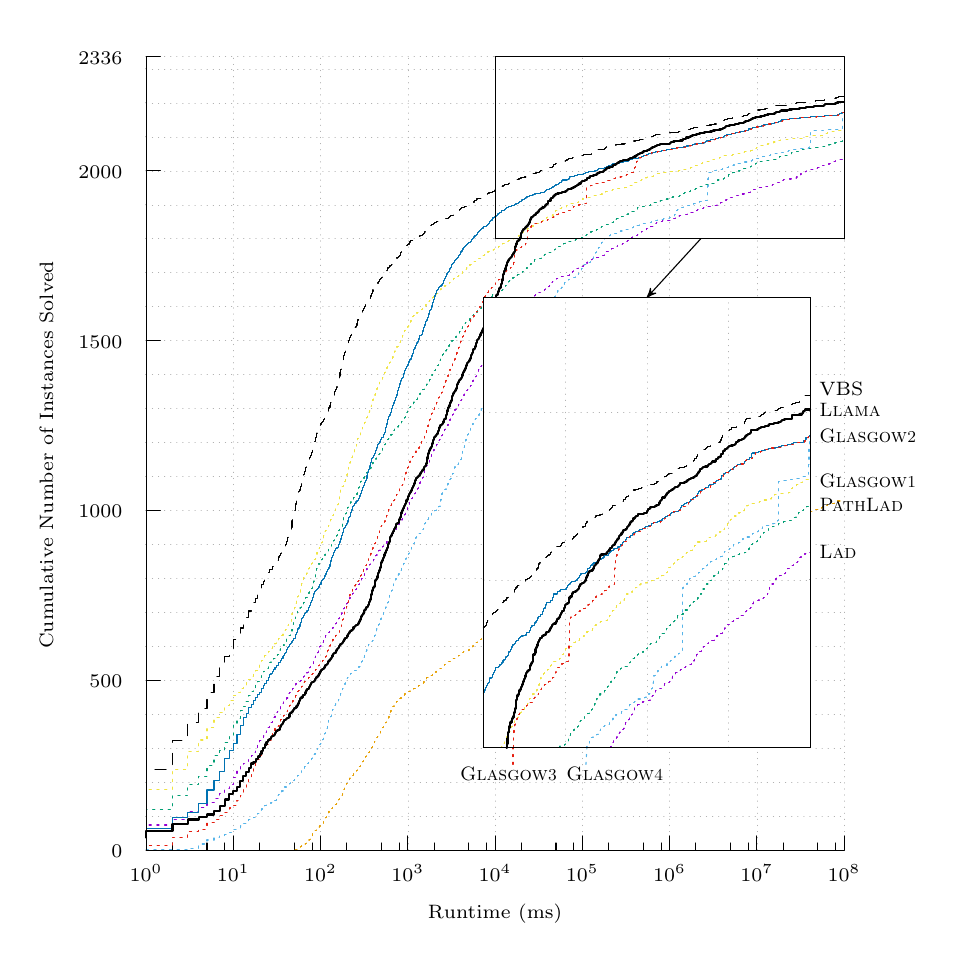
\begin{tikzpicture}[gnuplot]
%% generated with GNUPLOT 5.0p0 (Lua 5.2; terminal rev. 99, script rev. 100)
%% Wed 13 Apr 2016 09:44:01 AEST
\tikzset{every node/.append style={font={\scriptsize}}}
\path (0.000,0.000) rectangle (10.922,11.430);
\gpcolor{color=gp lt color axes}
\gpsetlinetype{gp lt axes}
\gpsetdashtype{gp dt axes}
\gpsetlinewidth{0.50}
\draw[gp path] (1.504,11.061)--(10.368,11.061);
\gpcolor{color=gp lt color border}
\gpsetlinetype{gp lt border}
\gpsetdashtype{gp dt solid}
\gpsetlinewidth{1.00}
\draw[gp path] (1.504,11.061)--(1.684,11.061);
\node[gp node right] at (1.320,11.061) {$2336$};
\gpcolor{color=gp lt color axes}
\gpsetlinetype{gp lt axes}
\gpsetdashtype{gp dt axes}
\gpsetlinewidth{0.50}
\draw[gp path] (1.504,0.985)--(10.368,0.985);
\gpcolor{color=gp lt color border}
\gpsetlinetype{gp lt border}
\gpsetdashtype{gp dt solid}
\gpsetlinewidth{1.00}
\draw[gp path] (1.504,0.985)--(1.684,0.985);
\node[gp node right] at (1.320,0.985) {$0$};
\gpcolor{color=gp lt color axes}
\gpsetlinetype{gp lt axes}
\gpsetdashtype{gp dt axes}
\gpsetlinewidth{0.50}
\draw[gp path] (1.504,1.416)--(10.368,1.416);
\gpcolor{color=gp lt color border}
\gpsetlinetype{gp lt border}
\gpsetdashtype{gp dt solid}
\gpsetlinewidth{1.00}
\draw[gp path] (1.504,1.416)--(1.505,1.416);
\gpcolor{color=gp lt color axes}
\gpsetlinetype{gp lt axes}
\gpsetdashtype{gp dt axes}
\gpsetlinewidth{0.50}
\draw[gp path] (1.504,1.848)--(10.368,1.848);
\gpcolor{color=gp lt color border}
\gpsetlinetype{gp lt border}
\gpsetdashtype{gp dt solid}
\gpsetlinewidth{1.00}
\draw[gp path] (1.504,1.848)--(1.505,1.848);
\gpcolor{color=gp lt color axes}
\gpsetlinetype{gp lt axes}
\gpsetdashtype{gp dt axes}
\gpsetlinewidth{0.50}
\draw[gp path] (1.504,2.279)--(10.368,2.279);
\gpcolor{color=gp lt color border}
\gpsetlinetype{gp lt border}
\gpsetdashtype{gp dt solid}
\gpsetlinewidth{1.00}
\draw[gp path] (1.504,2.279)--(1.505,2.279);
\gpcolor{color=gp lt color axes}
\gpsetlinetype{gp lt axes}
\gpsetdashtype{gp dt axes}
\gpsetlinewidth{0.50}
\draw[gp path] (1.504,2.710)--(10.368,2.710);
\gpcolor{color=gp lt color border}
\gpsetlinetype{gp lt border}
\gpsetdashtype{gp dt solid}
\gpsetlinewidth{1.00}
\draw[gp path] (1.504,2.710)--(1.505,2.710);
\gpcolor{color=gp lt color axes}
\gpsetlinetype{gp lt axes}
\gpsetdashtype{gp dt axes}
\gpsetlinewidth{0.50}
\draw[gp path] (1.504,3.142)--(10.368,3.142);
\gpcolor{color=gp lt color border}
\gpsetlinetype{gp lt border}
\gpsetdashtype{gp dt solid}
\gpsetlinewidth{1.00}
\draw[gp path] (1.504,3.142)--(1.684,3.142);
\node[gp node right] at (1.320,3.142) {$500$};
\gpcolor{color=gp lt color axes}
\gpsetlinetype{gp lt axes}
\gpsetdashtype{gp dt axes}
\gpsetlinewidth{0.50}
\draw[gp path] (1.504,3.573)--(10.368,3.573);
\gpcolor{color=gp lt color border}
\gpsetlinetype{gp lt border}
\gpsetdashtype{gp dt solid}
\gpsetlinewidth{1.00}
\draw[gp path] (1.504,3.573)--(1.505,3.573);
\gpcolor{color=gp lt color axes}
\gpsetlinetype{gp lt axes}
\gpsetdashtype{gp dt axes}
\gpsetlinewidth{0.50}
\draw[gp path] (1.504,4.004)--(10.368,4.004);
\gpcolor{color=gp lt color border}
\gpsetlinetype{gp lt border}
\gpsetdashtype{gp dt solid}
\gpsetlinewidth{1.00}
\draw[gp path] (1.504,4.004)--(1.505,4.004);
\gpcolor{color=gp lt color axes}
\gpsetlinetype{gp lt axes}
\gpsetdashtype{gp dt axes}
\gpsetlinewidth{0.50}
\draw[gp path] (1.504,4.436)--(10.368,4.436);
\gpcolor{color=gp lt color border}
\gpsetlinetype{gp lt border}
\gpsetdashtype{gp dt solid}
\gpsetlinewidth{1.00}
\draw[gp path] (1.504,4.436)--(1.505,4.436);
\gpcolor{color=gp lt color axes}
\gpsetlinetype{gp lt axes}
\gpsetdashtype{gp dt axes}
\gpsetlinewidth{0.50}
\draw[gp path] (1.504,4.867)--(10.368,4.867);
\gpcolor{color=gp lt color border}
\gpsetlinetype{gp lt border}
\gpsetdashtype{gp dt solid}
\gpsetlinewidth{1.00}
\draw[gp path] (1.504,4.867)--(1.505,4.867);
\gpcolor{color=gp lt color axes}
\gpsetlinetype{gp lt axes}
\gpsetdashtype{gp dt axes}
\gpsetlinewidth{0.50}
\draw[gp path] (1.504,5.298)--(10.368,5.298);
\gpcolor{color=gp lt color border}
\gpsetlinetype{gp lt border}
\gpsetdashtype{gp dt solid}
\gpsetlinewidth{1.00}
\draw[gp path] (1.504,5.298)--(1.684,5.298);
\node[gp node right] at (1.320,5.298) {$1000$};
\gpcolor{color=gp lt color axes}
\gpsetlinetype{gp lt axes}
\gpsetdashtype{gp dt axes}
\gpsetlinewidth{0.50}
\draw[gp path] (1.504,5.730)--(10.368,5.730);
\gpcolor{color=gp lt color border}
\gpsetlinetype{gp lt border}
\gpsetdashtype{gp dt solid}
\gpsetlinewidth{1.00}
\draw[gp path] (1.504,5.730)--(1.505,5.730);
\gpcolor{color=gp lt color axes}
\gpsetlinetype{gp lt axes}
\gpsetdashtype{gp dt axes}
\gpsetlinewidth{0.50}
\draw[gp path] (1.504,6.161)--(10.368,6.161);
\gpcolor{color=gp lt color border}
\gpsetlinetype{gp lt border}
\gpsetdashtype{gp dt solid}
\gpsetlinewidth{1.00}
\draw[gp path] (1.504,6.161)--(1.505,6.161);
\gpcolor{color=gp lt color axes}
\gpsetlinetype{gp lt axes}
\gpsetdashtype{gp dt axes}
\gpsetlinewidth{0.50}
\draw[gp path] (1.504,6.592)--(10.368,6.592);
\gpcolor{color=gp lt color border}
\gpsetlinetype{gp lt border}
\gpsetdashtype{gp dt solid}
\gpsetlinewidth{1.00}
\draw[gp path] (1.504,6.592)--(1.505,6.592);
\gpcolor{color=gp lt color axes}
\gpsetlinetype{gp lt axes}
\gpsetdashtype{gp dt axes}
\gpsetlinewidth{0.50}
\draw[gp path] (1.504,7.024)--(10.368,7.024);
\gpcolor{color=gp lt color border}
\gpsetlinetype{gp lt border}
\gpsetdashtype{gp dt solid}
\gpsetlinewidth{1.00}
\draw[gp path] (1.504,7.024)--(1.505,7.024);
\gpcolor{color=gp lt color axes}
\gpsetlinetype{gp lt axes}
\gpsetdashtype{gp dt axes}
\gpsetlinewidth{0.50}
\draw[gp path] (1.504,7.455)--(10.368,7.455);
\gpcolor{color=gp lt color border}
\gpsetlinetype{gp lt border}
\gpsetdashtype{gp dt solid}
\gpsetlinewidth{1.00}
\draw[gp path] (1.504,7.455)--(1.684,7.455);
\node[gp node right] at (1.320,7.455) {$1500$};
\gpcolor{color=gp lt color axes}
\gpsetlinetype{gp lt axes}
\gpsetdashtype{gp dt axes}
\gpsetlinewidth{0.50}
\draw[gp path] (1.504,7.886)--(10.368,7.886);
\gpcolor{color=gp lt color border}
\gpsetlinetype{gp lt border}
\gpsetdashtype{gp dt solid}
\gpsetlinewidth{1.00}
\draw[gp path] (1.504,7.886)--(1.505,7.886);
\gpcolor{color=gp lt color axes}
\gpsetlinetype{gp lt axes}
\gpsetdashtype{gp dt axes}
\gpsetlinewidth{0.50}
\draw[gp path] (1.504,8.318)--(10.368,8.318);
\gpcolor{color=gp lt color border}
\gpsetlinetype{gp lt border}
\gpsetdashtype{gp dt solid}
\gpsetlinewidth{1.00}
\draw[gp path] (1.504,8.318)--(1.505,8.318);
\gpcolor{color=gp lt color axes}
\gpsetlinetype{gp lt axes}
\gpsetdashtype{gp dt axes}
\gpsetlinewidth{0.50}
\draw[gp path] (1.504,8.749)--(10.368,8.749);
\gpcolor{color=gp lt color border}
\gpsetlinetype{gp lt border}
\gpsetdashtype{gp dt solid}
\gpsetlinewidth{1.00}
\draw[gp path] (1.504,8.749)--(1.505,8.749);
\gpcolor{color=gp lt color axes}
\gpsetlinetype{gp lt axes}
\gpsetdashtype{gp dt axes}
\gpsetlinewidth{0.50}
\draw[gp path] (1.504,9.180)--(10.368,9.180);
\gpcolor{color=gp lt color border}
\gpsetlinetype{gp lt border}
\gpsetdashtype{gp dt solid}
\gpsetlinewidth{1.00}
\draw[gp path] (1.504,9.180)--(1.505,9.180);
\gpcolor{color=gp lt color axes}
\gpsetlinetype{gp lt axes}
\gpsetdashtype{gp dt axes}
\gpsetlinewidth{0.50}
\draw[gp path] (1.504,9.612)--(10.368,9.612);
\gpcolor{color=gp lt color border}
\gpsetlinetype{gp lt border}
\gpsetdashtype{gp dt solid}
\gpsetlinewidth{1.00}
\draw[gp path] (1.504,9.612)--(1.684,9.612);
\node[gp node right] at (1.320,9.612) {$2000$};
\gpcolor{color=gp lt color axes}
\gpsetlinetype{gp lt axes}
\gpsetdashtype{gp dt axes}
\gpsetlinewidth{0.50}
\draw[gp path] (1.504,10.043)--(10.368,10.043);
\gpcolor{color=gp lt color border}
\gpsetlinetype{gp lt border}
\gpsetdashtype{gp dt solid}
\gpsetlinewidth{1.00}
\draw[gp path] (1.504,10.043)--(1.505,10.043);
\gpcolor{color=gp lt color axes}
\gpsetlinetype{gp lt axes}
\gpsetdashtype{gp dt axes}
\gpsetlinewidth{0.50}
\draw[gp path] (1.504,10.474)--(10.368,10.474);
\gpcolor{color=gp lt color border}
\gpsetlinetype{gp lt border}
\gpsetdashtype{gp dt solid}
\gpsetlinewidth{1.00}
\draw[gp path] (1.504,10.474)--(1.505,10.474);
\gpcolor{color=gp lt color axes}
\gpsetlinetype{gp lt axes}
\gpsetdashtype{gp dt axes}
\gpsetlinewidth{0.50}
\draw[gp path] (1.504,10.906)--(10.368,10.906);
\gpcolor{color=gp lt color border}
\gpsetlinetype{gp lt border}
\gpsetdashtype{gp dt solid}
\gpsetlinewidth{1.00}
\draw[gp path] (1.504,10.906)--(1.505,10.906);
\gpcolor{color=gp lt color axes}
\gpsetlinetype{gp lt axes}
\gpsetdashtype{gp dt axes}
\gpsetlinewidth{0.50}
\draw[gp path] (1.504,0.985)--(1.504,11.061);
\gpcolor{color=gp lt color border}
\gpsetlinetype{gp lt border}
\gpsetdashtype{gp dt solid}
\gpsetlinewidth{1.00}
\draw[gp path] (1.504,0.985)--(1.504,1.165);
\node[gp node center] at (1.504,0.677) {$10^{0}$};
\draw[gp path] (1.838,0.985)--(1.838,1.075);
\draw[gp path] (2.278,0.985)--(2.278,1.075);
\draw[gp path] (2.505,0.985)--(2.505,1.075);
\gpcolor{color=gp lt color axes}
\gpsetlinetype{gp lt axes}
\gpsetdashtype{gp dt axes}
\gpsetlinewidth{0.50}
\draw[gp path] (2.612,0.985)--(2.612,11.061);
\gpcolor{color=gp lt color border}
\gpsetlinetype{gp lt border}
\gpsetdashtype{gp dt solid}
\gpsetlinewidth{1.00}
\draw[gp path] (2.612,0.985)--(2.612,1.165);
\node[gp node center] at (2.612,0.677) {$10^{1}$};
\draw[gp path] (2.946,0.985)--(2.946,1.075);
\draw[gp path] (3.386,0.985)--(3.386,1.075);
\draw[gp path] (3.613,0.985)--(3.613,1.075);
\gpcolor{color=gp lt color axes}
\gpsetlinetype{gp lt axes}
\gpsetdashtype{gp dt axes}
\gpsetlinewidth{0.50}
\draw[gp path] (3.720,0.985)--(3.720,11.061);
\gpcolor{color=gp lt color border}
\gpsetlinetype{gp lt border}
\gpsetdashtype{gp dt solid}
\gpsetlinewidth{1.00}
\draw[gp path] (3.720,0.985)--(3.720,1.165);
\node[gp node center] at (3.720,0.677) {$10^{2}$};
\draw[gp path] (4.054,0.985)--(4.054,1.075);
\draw[gp path] (4.494,0.985)--(4.494,1.075);
\draw[gp path] (4.721,0.985)--(4.721,1.075);
\gpcolor{color=gp lt color axes}
\gpsetlinetype{gp lt axes}
\gpsetdashtype{gp dt axes}
\gpsetlinewidth{0.50}
\draw[gp path] (4.828,0.985)--(4.828,11.061);
\gpcolor{color=gp lt color border}
\gpsetlinetype{gp lt border}
\gpsetdashtype{gp dt solid}
\gpsetlinewidth{1.00}
\draw[gp path] (4.828,0.985)--(4.828,1.165);
\node[gp node center] at (4.828,0.677) {$10^{3}$};
\draw[gp path] (5.162,0.985)--(5.162,1.075);
\draw[gp path] (5.602,0.985)--(5.602,1.075);
\draw[gp path] (5.829,0.985)--(5.829,1.075);
\gpcolor{color=gp lt color axes}
\gpsetlinetype{gp lt axes}
\gpsetdashtype{gp dt axes}
\gpsetlinewidth{0.50}
\draw[gp path] (5.936,0.985)--(5.936,11.061);
\gpcolor{color=gp lt color border}
\gpsetlinetype{gp lt border}
\gpsetdashtype{gp dt solid}
\gpsetlinewidth{1.00}
\draw[gp path] (5.936,0.985)--(5.936,1.165);
\node[gp node center] at (5.936,0.677) {$10^{4}$};
\draw[gp path] (6.270,0.985)--(6.270,1.075);
\draw[gp path] (6.710,0.985)--(6.710,1.075);
\draw[gp path] (6.937,0.985)--(6.937,1.075);
\gpcolor{color=gp lt color axes}
\gpsetlinetype{gp lt axes}
\gpsetdashtype{gp dt axes}
\gpsetlinewidth{0.50}
\draw[gp path] (7.044,0.985)--(7.044,11.061);
\gpcolor{color=gp lt color border}
\gpsetlinetype{gp lt border}
\gpsetdashtype{gp dt solid}
\gpsetlinewidth{1.00}
\draw[gp path] (7.044,0.985)--(7.044,1.165);
\node[gp node center] at (7.044,0.677) {$10^{5}$};
\draw[gp path] (7.378,0.985)--(7.378,1.075);
\draw[gp path] (7.818,0.985)--(7.818,1.075);
\draw[gp path] (8.045,0.985)--(8.045,1.075);
\gpcolor{color=gp lt color axes}
\gpsetlinetype{gp lt axes}
\gpsetdashtype{gp dt axes}
\gpsetlinewidth{0.50}
\draw[gp path] (8.152,0.985)--(8.152,11.061);
\gpcolor{color=gp lt color border}
\gpsetlinetype{gp lt border}
\gpsetdashtype{gp dt solid}
\gpsetlinewidth{1.00}
\draw[gp path] (8.152,0.985)--(8.152,1.165);
\node[gp node center] at (8.152,0.677) {$10^{6}$};
\draw[gp path] (8.486,0.985)--(8.486,1.075);
\draw[gp path] (8.926,0.985)--(8.926,1.075);
\draw[gp path] (9.153,0.985)--(9.153,1.075);
\gpcolor{color=gp lt color axes}
\gpsetlinetype{gp lt axes}
\gpsetdashtype{gp dt axes}
\gpsetlinewidth{0.50}
\draw[gp path] (9.260,0.985)--(9.260,11.061);
\gpcolor{color=gp lt color border}
\gpsetlinetype{gp lt border}
\gpsetdashtype{gp dt solid}
\gpsetlinewidth{1.00}
\draw[gp path] (9.260,0.985)--(9.260,1.165);
\node[gp node center] at (9.260,0.677) {$10^{7}$};
\draw[gp path] (9.594,0.985)--(9.594,1.075);
\draw[gp path] (10.034,0.985)--(10.034,1.075);
\draw[gp path] (10.261,0.985)--(10.261,1.075);
\gpcolor{color=gp lt color axes}
\gpsetlinetype{gp lt axes}
\gpsetdashtype{gp dt axes}
\gpsetlinewidth{0.50}
\draw[gp path] (10.368,0.985)--(10.368,11.061);
\gpcolor{color=gp lt color border}
\gpsetlinetype{gp lt border}
\gpsetdashtype{gp dt solid}
\gpsetlinewidth{1.00}
\draw[gp path] (10.368,0.985)--(10.368,1.165);
\node[gp node center] at (10.368,0.677) {$10^{8}$};
\draw[gp path] (1.504,11.061)--(1.504,0.985)--(10.368,0.985);
\node[gp node center,rotate=-270] at (0.246,6.023) {Cumulative Number of Instances Solved};
\node[gp node center] at (5.936,0.215) {Runtime (ms)};
\gpcolor{rgb color={0.580,0.000,0.827}}
\gpsetdashtype{dash pattern=on 2.00*\gpdashlength off 5.00*\gpdashlength }
\draw[gp path] (1.504,1.145)--(1.504,1.304)--(1.838,1.304)--(1.838,1.378)--(2.033,1.378)%
  --(2.033,1.472)--(2.171,1.472)--(2.171,1.524)--(2.278,1.524)--(2.278,1.585)--(2.366,1.585)%
  --(2.366,1.636)--(2.440,1.636)--(2.440,1.705)--(2.505,1.705)--(2.505,1.766)--(2.561,1.766)%
  --(2.561,1.817)--(2.612,1.817)--(2.612,1.908)--(2.658,1.908)--(2.658,1.990)--(2.700,1.990)%
  --(2.700,2.059)--(2.738,2.059)--(2.738,2.089)--(2.774,2.089)--(2.774,2.106)--(2.807,2.106)%
  --(2.807,2.141)--(2.838,2.141)--(2.838,2.184)--(2.867,2.184)--(2.867,2.219)--(2.895,2.219)%
  --(2.895,2.283)--(2.921,2.283)--(2.921,2.331)--(2.946,2.331)--(2.946,2.374)--(2.969,2.374)%
  --(2.969,2.408)--(2.991,2.408)--(2.991,2.434)--(3.013,2.434)--(3.013,2.473)--(3.033,2.473)%
  --(3.033,2.508)--(3.053,2.508)--(3.053,2.546)--(3.072,2.546)--(3.072,2.585)--(3.090,2.585)%
  --(3.090,2.607)--(3.107,2.607)--(3.107,2.646)--(3.124,2.646)--(3.124,2.672)--(3.141,2.672)%
  --(3.141,2.706)--(3.156,2.706)--(3.156,2.732)--(3.172,2.732)--(3.172,2.749)--(3.187,2.749)%
  --(3.187,2.753)--(3.201,2.753)--(3.201,2.775)--(3.215,2.775)--(3.215,2.810)--(3.228,2.810)%
  --(3.228,2.835)--(3.242,2.835)--(3.242,2.848)--(3.254,2.848)--(3.254,2.870)--(3.267,2.870)%
  --(3.267,2.883)--(3.279,2.883)--(3.279,2.900)--(3.291,2.900)--(3.291,2.917)--(3.303,2.917)%
  --(3.303,2.952)--(3.314,2.952)--(3.314,2.973)--(3.325,2.973)--(3.325,2.982)--(3.346,2.982)%
  --(3.346,2.986)--(3.357,2.986)--(3.357,3.012)--(3.367,3.012)--(3.367,3.038)--(3.377,3.038)%
  --(3.377,3.042)--(3.386,3.042)--(3.386,3.068)--(3.396,3.068)--(3.396,3.081)--(3.405,3.081)%
  --(3.405,3.094)--(3.414,3.094)--(3.414,3.107)--(3.432,3.107)--(3.432,3.120)--(3.450,3.120)%
  --(3.450,3.124)--(3.458,3.124)--(3.458,3.129)--(3.466,3.129)--(3.466,3.137)--(3.474,3.137)%
  --(3.474,3.159)--(3.482,3.159)--(3.482,3.163)--(3.490,3.163)--(3.490,3.168)--(3.505,3.168)%
  --(3.505,3.185)--(3.513,3.185)--(3.513,3.211)--(3.527,3.211)--(3.527,3.215)--(3.534,3.215)%
  --(3.534,3.219)--(3.541,3.219)--(3.541,3.232)--(3.548,3.232)--(3.548,3.245)--(3.562,3.245)%
  --(3.562,3.254)--(3.569,3.254)--(3.569,3.262)--(3.575,3.262)--(3.575,3.271)--(3.582,3.271)%
  --(3.582,3.301)--(3.588,3.301)--(3.588,3.314)--(3.594,3.314)--(3.594,3.319)--(3.600,3.319)%
  --(3.600,3.331)--(3.607,3.331)--(3.607,3.340)--(3.613,3.340)--(3.613,3.349)--(3.625,3.349)%
  --(3.625,3.362)--(3.630,3.362)--(3.630,3.383)--(3.636,3.383)--(3.636,3.396)--(3.642,3.396)%
  --(3.642,3.409)--(3.647,3.409)--(3.647,3.426)--(3.653,3.426)--(3.653,3.439)--(3.658,3.439)%
  --(3.658,3.448)--(3.664,3.448)--(3.664,3.457)--(3.669,3.457)--(3.669,3.465)--(3.675,3.465)%
  --(3.675,3.474)--(3.680,3.474)--(3.680,3.482)--(3.685,3.482)--(3.685,3.491)--(3.690,3.491)%
  --(3.690,3.530)--(3.695,3.530)--(3.695,3.534)--(3.700,3.534)--(3.700,3.547)--(3.705,3.547)%
  --(3.705,3.551)--(3.710,3.551)--(3.710,3.569)--(3.715,3.569)--(3.715,3.573)--(3.720,3.573)%
  --(3.720,3.577)--(3.730,3.577)--(3.730,3.582)--(3.734,3.582)--(3.734,3.590)--(3.739,3.590)%
  --(3.739,3.608)--(3.743,3.608)--(3.743,3.612)--(3.748,3.612)--(3.748,3.620)--(3.753,3.620)%
  --(3.753,3.629)--(3.757,3.629)--(3.757,3.642)--(3.766,3.642)--(3.766,3.646)--(3.770,3.646)%
  --(3.770,3.659)--(3.775,3.659)--(3.775,3.681)--(3.779,3.681)--(3.779,3.685)--(3.783,3.685)%
  --(3.783,3.707)--(3.787,3.707)--(3.787,3.711)--(3.791,3.711)--(3.791,3.720)--(3.796,3.720)%
  --(3.796,3.724)--(3.804,3.724)--(3.804,3.728)--(3.808,3.728)--(3.808,3.733)--(3.812,3.733)%
  --(3.812,3.741)--(3.816,3.741)--(3.816,3.746)--(3.820,3.746)--(3.820,3.750)--(3.824,3.750)%
  --(3.824,3.754)--(3.831,3.754)--(3.831,3.763)--(3.835,3.763)--(3.835,3.767)--(3.843,3.767)%
  --(3.843,3.771)--(3.846,3.771)--(3.846,3.780)--(3.854,3.780)--(3.854,3.784)--(3.861,3.784)%
  --(3.861,3.789)--(3.864,3.789)--(3.864,3.793)--(3.868,3.793)--(3.868,3.797)--(3.871,3.797)%
  --(3.871,3.802)--(3.875,3.802)--(3.875,3.806)--(3.878,3.806)--(3.878,3.810)--(3.882,3.810)%
  --(3.882,3.815)--(3.885,3.815)--(3.885,3.828)--(3.895,3.828)--(3.895,3.840)--(3.899,3.840)%
  --(3.899,3.849)--(3.905,3.849)--(3.905,3.853)--(3.909,3.853)--(3.909,3.858)--(3.915,3.858)%
  --(3.915,3.866)--(3.918,3.866)--(3.918,3.875)--(3.921,3.875)--(3.921,3.888)--(3.925,3.888)%
  --(3.925,3.892)--(3.928,3.892)--(3.928,3.901)--(3.934,3.901)--(3.934,3.909)--(3.940,3.909)%
  --(3.940,3.914)--(3.943,3.914)--(3.943,3.922)--(3.949,3.922)--(3.949,3.927)--(3.952,3.927)%
  --(3.952,3.931)--(3.955,3.931)--(3.955,3.935)--(3.958,3.935)--(3.958,3.940)--(3.964,3.940)%
  --(3.964,3.944)--(3.967,3.944)--(3.967,3.948)--(3.970,3.948)--(3.970,3.953)--(3.972,3.953)%
  --(3.972,3.957)--(3.975,3.957)--(3.975,3.961)--(3.981,3.961)--(3.981,3.966)--(3.984,3.966)%
  --(3.984,3.970)--(3.987,3.970)--(3.987,3.978)--(3.989,3.978)--(3.989,3.991)--(3.992,3.991)%
  --(3.992,4.000)--(4.000,4.000)--(4.000,4.009)--(4.003,4.009)--(4.003,4.030)--(4.006,4.030)%
  --(4.006,4.039)--(4.008,4.039)--(4.008,4.043)--(4.011,4.043)--(4.011,4.047)--(4.013,4.047)%
  --(4.013,4.052)--(4.019,4.052)--(4.019,4.056)--(4.021,4.056)--(4.021,4.069)--(4.024,4.069)%
  --(4.024,4.073)--(4.026,4.073)--(4.026,4.078)--(4.031,4.078)--(4.031,4.082)--(4.036,4.082)%
  --(4.036,4.086)--(4.041,4.086)--(4.041,4.099)--(4.044,4.099)--(4.044,4.104)--(4.049,4.104)%
  --(4.049,4.108)--(4.051,4.108)--(4.051,4.112)--(4.054,4.112)--(4.054,4.116)--(4.056,4.116)%
  --(4.056,4.121)--(4.058,4.121)--(4.058,4.125)--(4.061,4.125)--(4.061,4.129)--(4.063,4.129)%
  --(4.063,4.134)--(4.068,4.134)--(4.068,4.142)--(4.070,4.142)--(4.070,4.151)--(4.077,4.151)%
  --(4.077,4.164)--(4.082,4.164)--(4.082,4.177)--(4.086,4.177)--(4.086,4.181)--(4.091,4.181)%
  --(4.091,4.186)--(4.093,4.186)--(4.093,4.194)--(4.097,4.194)--(4.097,4.198)--(4.102,4.198)%
  --(4.102,4.211)--(4.110,4.211)--(4.110,4.220)--(4.112,4.220)--(4.112,4.224)--(4.119,4.224)%
  --(4.119,4.229)--(4.121,4.229)--(4.121,4.233)--(4.123,4.233)--(4.123,4.237)--(4.129,4.237)%
  --(4.129,4.242)--(4.133,4.242)--(4.133,4.246)--(4.135,4.246)--(4.135,4.250)--(4.139,4.250)%
  --(4.139,4.259)--(4.141,4.259)--(4.141,4.267)--(4.149,4.267)--(4.149,4.276)--(4.155,4.276)%
  --(4.155,4.285)--(4.157,4.285)--(4.157,4.289)--(4.163,4.289)--(4.163,4.293)--(4.172,4.293)%
  --(4.172,4.298)--(4.174,4.298)--(4.174,4.306)--(4.180,4.306)--(4.180,4.315)--(4.183,4.315)%
  --(4.183,4.319)--(4.191,4.319)--(4.191,4.324)--(4.193,4.324)--(4.193,4.332)--(4.194,4.332)%
  --(4.194,4.341)--(4.196,4.341)--(4.196,4.349)--(4.198,4.349)--(4.198,4.354)--(4.200,4.354)%
  --(4.200,4.358)--(4.207,4.358)--(4.207,4.362)--(4.210,4.362)--(4.210,4.371)--(4.212,4.371)%
  --(4.212,4.380)--(4.215,4.380)--(4.215,4.384)--(4.219,4.384)--(4.219,4.388)--(4.221,4.388)%
  --(4.221,4.393)--(4.222,4.393)--(4.222,4.397)--(4.224,4.397)--(4.224,4.401)--(4.227,4.401)%
  --(4.227,4.405)--(4.234,4.405)--(4.234,4.410)--(4.236,4.410)--(4.236,4.418)--(4.241,4.418)%
  --(4.241,4.427)--(4.242,4.427)--(4.242,4.431)--(4.255,4.431)--(4.255,4.440)--(4.258,4.440)%
  --(4.258,4.444)--(4.260,4.444)--(4.260,4.449)--(4.261,4.449)--(4.261,4.462)--(4.263,4.462)%
  --(4.263,4.466)--(4.271,4.466)--(4.271,4.470)--(4.275,4.470)--(4.275,4.475)--(4.277,4.475)%
  --(4.277,4.479)--(4.278,4.479)--(4.278,4.483)--(4.280,4.483)--(4.280,4.487)--(4.283,4.487)%
  --(4.283,4.496)--(4.289,4.496)--(4.289,4.500)--(4.292,4.500)--(4.292,4.509)--(4.293,4.509)%
  --(4.293,4.513)--(4.296,4.513)--(4.296,4.526)--(4.299,4.526)--(4.299,4.531)--(4.303,4.531)%
  --(4.303,4.535)--(4.305,4.535)--(4.305,4.544)--(4.306,4.544)--(4.306,4.548)--(4.307,4.548)%
  --(4.307,4.552)--(4.309,4.552)--(4.309,4.556)--(4.310,4.556)--(4.310,4.565)--(4.319,4.565)%
  --(4.319,4.569)--(4.320,4.569)--(4.320,4.574)--(4.321,4.574)--(4.321,4.578)--(4.323,4.578)%
  --(4.323,4.582)--(4.326,4.582)--(4.326,4.587)--(4.327,4.587)--(4.327,4.591)--(4.328,4.591)%
  --(4.328,4.595)--(4.338,4.595)--(4.338,4.604)--(4.343,4.604)--(4.343,4.608)--(4.346,4.608)%
  --(4.346,4.617)--(4.355,4.617)--(4.355,4.621)--(4.359,4.621)--(4.359,4.630)--(4.369,4.630)%
  --(4.369,4.634)--(4.370,4.634)--(4.370,4.638)--(4.371,4.638)--(4.371,4.643)--(4.375,4.643)%
  --(4.375,4.647)--(4.379,4.647)--(4.379,4.651)--(4.381,4.651)--(4.381,4.656)--(4.388,4.656)%
  --(4.388,4.660)--(4.389,4.660)--(4.389,4.664)--(4.394,4.664)--(4.394,4.669)--(4.397,4.669)%
  --(4.397,4.673)--(4.402,4.673)--(4.402,4.677)--(4.405,4.677)--(4.405,4.682)--(4.406,4.682)%
  --(4.406,4.686)--(4.407,4.686)--(4.407,4.690)--(4.409,4.690)--(4.409,4.694)--(4.412,4.694)%
  --(4.412,4.699)--(4.414,4.699)--(4.414,4.703)--(4.415,4.703)--(4.415,4.712)--(4.417,4.712)%
  --(4.417,4.716)--(4.420,4.716)--(4.420,4.720)--(4.421,4.720)--(4.421,4.725)--(4.423,4.725)%
  --(4.423,4.729)--(4.430,4.729)--(4.430,4.733)--(4.437,4.733)--(4.437,4.738)--(4.441,4.738)%
  --(4.441,4.742)--(4.443,4.742)--(4.443,4.746)--(4.445,4.746)--(4.445,4.751)--(4.447,4.751)%
  --(4.447,4.755)--(4.448,4.755)--(4.448,4.764)--(4.452,4.764)--(4.452,4.768)--(4.453,4.768)%
  --(4.453,4.772)--(4.454,4.772)--(4.454,4.776)--(4.459,4.776)--(4.459,4.781)--(4.460,4.781)%
  --(4.460,4.785)--(4.470,4.785)--(4.470,4.794)--(4.475,4.794)--(4.475,4.798)--(4.482,4.798)%
  --(4.482,4.802)--(4.483,4.802)--(4.483,4.807)--(4.491,4.807)--(4.491,4.811)--(4.496,4.811)%
  --(4.496,4.820)--(4.498,4.820)--(4.498,4.824)--(4.499,4.824)--(4.499,4.828)--(4.501,4.828)%
  --(4.501,4.833)--(4.507,4.833)--(4.507,4.837)--(4.508,4.837)--(4.508,4.841)--(4.518,4.841)%
  --(4.518,4.845)--(4.519,4.845)--(4.519,4.850)--(4.523,4.850)--(4.523,4.854)--(4.529,4.854)%
  --(4.529,4.858)--(4.530,4.858)--(4.530,4.863)--(4.542,4.863)--(4.542,4.867)--(4.544,4.867)%
  --(4.544,4.876)--(4.547,4.876)--(4.547,4.880)--(4.551,4.880)--(4.551,4.884)--(4.557,4.884)%
  --(4.557,4.889)--(4.558,4.889)--(4.558,4.893)--(4.561,4.893)--(4.561,4.897)--(4.563,4.897)%
  --(4.563,4.902)--(4.564,4.902)--(4.564,4.906)--(4.567,4.906)--(4.567,4.910)--(4.577,4.910)%
  --(4.577,4.914)--(4.580,4.914)--(4.580,4.923)--(4.582,4.923)--(4.582,4.927)--(4.586,4.927)%
  --(4.586,4.932)--(4.587,4.932)--(4.587,4.936)--(4.590,4.936)--(4.590,4.940)--(4.593,4.940)%
  --(4.593,4.949)--(4.599,4.949)--(4.599,4.953)--(4.600,4.953)--(4.600,4.958)--(4.603,4.958)%
  --(4.603,4.962)--(4.604,4.962)--(4.604,4.971)--(4.609,4.971)--(4.609,4.975)--(4.620,4.975)%
  --(4.620,4.979)--(4.621,4.979)--(4.621,4.983)--(4.623,4.983)--(4.623,4.988)--(4.628,4.988)%
  --(4.628,4.992)--(4.635,4.992)--(4.635,4.996)--(4.636,4.996)--(4.636,5.001)--(4.637,5.001)%
  --(4.637,5.005)--(4.641,5.005)--(4.641,5.009)--(4.644,5.009)--(4.644,5.014)--(4.649,5.014)%
  --(4.649,5.018)--(4.653,5.018)--(4.653,5.022)--(4.656,5.022)--(4.656,5.027)--(4.657,5.027)%
  --(4.657,5.035)--(4.658,5.035)--(4.658,5.040)--(4.661,5.040)--(4.661,5.044)--(4.669,5.044)%
  --(4.669,5.048)--(4.669,5.052)--(4.671,5.052)--(4.671,5.057)--(4.679,5.057)--(4.679,5.061)%
  --(4.679,5.065)--(4.684,5.065)--(4.684,5.070)--(4.686,5.070)--(4.686,5.074)--(4.686,5.078)%
  --(4.688,5.078)--(4.688,5.083)--(4.691,5.083)--(4.691,5.087)--(4.693,5.087)--(4.693,5.091)%
  --(4.693,5.096)--(4.706,5.096)--(4.706,5.100)--(4.707,5.100)--(4.707,5.104)--(4.709,5.104)%
  --(4.709,5.109)--(4.710,5.109)--(4.710,5.113)--(4.711,5.113)--(4.711,5.122)--(4.719,5.122)%
  --(4.719,5.126)--(4.722,5.126)--(4.722,5.130)--(4.723,5.130)--(4.723,5.134)--(4.726,5.134)%
  --(4.726,5.139)--(4.728,5.139)--(4.728,5.147)--(4.729,5.147)--(4.729,5.152)--(4.732,5.152)%
  --(4.732,5.156)--(4.734,5.156)--(4.734,5.160)--(4.743,5.160)--(4.743,5.165)--(4.745,5.165)%
  --(4.745,5.169)--(4.753,5.169)--(4.753,5.173)--(4.754,5.173)--(4.754,5.182)--(4.754,5.186)%
  --(4.757,5.186)--(4.757,5.191)--(4.763,5.191)--(4.763,5.199)--(4.764,5.199)--(4.764,5.203)%
  --(4.766,5.203)--(4.766,5.208)--(4.767,5.208)--(4.767,5.212)--(4.768,5.212)--(4.768,5.216)%
  --(4.769,5.216)--(4.769,5.221)--(4.770,5.221)--(4.770,5.225)--(4.772,5.225)--(4.772,5.234)%
  --(4.783,5.234)--(4.783,5.238)--(4.789,5.238)--(4.789,5.242)--(4.789,5.247)--(4.792,5.247)%
  --(4.792,5.251)--(4.794,5.251)--(4.794,5.255)--(4.794,5.260)--(4.795,5.260)--(4.795,5.264)%
  --(4.796,5.264)--(4.796,5.268)--(4.798,5.268)--(4.798,5.272)--(4.800,5.272)--(4.800,5.277)%
  --(4.804,5.277)--(4.804,5.281)--(4.807,5.281)--(4.807,5.290)--(4.809,5.290)--(4.809,5.294)%
  --(4.810,5.294)--(4.810,5.298)--(4.812,5.298)--(4.812,5.303)--(4.816,5.303)--(4.816,5.307)%
  --(4.819,5.307)--(4.819,5.316)--(4.821,5.316)--(4.821,5.320)--(4.821,5.324)--(4.822,5.324)%
  --(4.822,5.329)--(4.823,5.329)--(4.823,5.333)--(4.823,5.337)--(4.827,5.337)--(4.827,5.341)%
  --(4.832,5.341)--(4.832,5.346)--(4.833,5.346)--(4.833,5.350)--(4.837,5.350)--(4.837,5.354)%
  --(4.838,5.354)--(4.838,5.363)--(4.840,5.363)--(4.840,5.367)--(4.843,5.367)--(4.843,5.372)%
  --(4.848,5.372)--(4.848,5.376)--(4.849,5.376)--(4.849,5.380)--(4.850,5.380)--(4.850,5.385)%
  --(4.851,5.385)--(4.851,5.389)--(4.851,5.393)--(4.852,5.393)--(4.852,5.398)--(4.853,5.398)%
  --(4.853,5.411)--(4.855,5.411)--(4.855,5.419)--(4.856,5.419)--(4.856,5.423)--(4.861,5.423)%
  --(4.861,5.428)--(4.865,5.428)--(4.865,5.432)--(4.869,5.432)--(4.869,5.436)--(4.869,5.441)%
  --(4.873,5.441)--(4.873,5.445)--(4.876,5.445)--(4.876,5.449)--(4.882,5.449)--(4.882,5.454)%
  --(4.886,5.454)--(4.886,5.458)--(4.886,5.462)--(4.889,5.462)--(4.889,5.467)--(4.893,5.467)%
  --(4.893,5.471)--(4.893,5.475)--(4.897,5.475)--(4.897,5.480)--(4.897,5.484)--(4.902,5.484)%
  --(4.902,5.492)--(4.904,5.492)--(4.904,5.497)--(4.906,5.497)--(4.906,5.505)--(4.907,5.505)%
  --(4.907,5.510)--(4.913,5.510)--(4.913,5.514)--(4.917,5.514)--(4.917,5.518)--(4.921,5.518)%
  --(4.921,5.523)--(4.921,5.527)--(4.926,5.527)--(4.926,5.531)--(4.927,5.531)--(4.927,5.536)%
  --(4.932,5.536)--(4.932,5.540)--(4.938,5.540)--(4.938,5.544)--(4.940,5.544)--(4.940,5.549)%
  --(4.941,5.549)--(4.941,5.553)--(4.943,5.553)--(4.943,5.557)--(4.944,5.557)--(4.944,5.561)%
  --(4.950,5.561)--(4.950,5.566)--(4.950,5.570)--(4.954,5.570)--(4.954,5.579)--(4.958,5.579)%
  --(4.958,5.583)--(4.958,5.587)--(4.960,5.587)--(4.960,5.592)--(4.963,5.592)--(4.963,5.596)%
  --(4.964,5.596)--(4.964,5.600)--(4.966,5.600)--(4.966,5.605)--(4.971,5.605)--(4.971,5.609)%
  --(4.972,5.609)--(4.972,5.613)--(4.973,5.613)--(4.973,5.618)--(4.974,5.618)--(4.974,5.622)%
  --(4.976,5.622)--(4.976,5.630)--(4.976,5.635)--(4.977,5.635)--(4.977,5.639)--(4.980,5.639)%
  --(4.980,5.643)--(4.982,5.643)--(4.982,5.648)--(4.983,5.648)--(4.983,5.652)--(4.984,5.652)%
  --(4.984,5.656)--(4.986,5.656)--(4.986,5.661)--(4.987,5.661)--(4.987,5.665)--(4.989,5.665)%
  --(4.989,5.669)--(4.991,5.669)--(4.991,5.674)--(4.994,5.674)--(4.994,5.678)--(4.998,5.678)%
  --(4.998,5.682)--(5.000,5.682)--(5.000,5.687)--(5.004,5.687)--(5.004,5.691)--(5.005,5.691)%
  --(5.005,5.695)--(5.005,5.699)--(5.011,5.699)--(5.011,5.708)--(5.016,5.708)--(5.016,5.712)%
  --(5.019,5.712)--(5.019,5.717)--(5.020,5.717)--(5.020,5.721)--(5.023,5.721)--(5.023,5.725)%
  --(5.025,5.725)--(5.025,5.734)--(5.026,5.734)--(5.026,5.738)--(5.026,5.743)--(5.030,5.743)%
  --(5.030,5.756)--(5.031,5.756)--(5.031,5.760)--(5.032,5.760)--(5.032,5.764)--(5.034,5.764)%
  --(5.034,5.773)--(5.036,5.773)--(5.036,5.781)--(5.037,5.781)--(5.037,5.786)--(5.039,5.786)%
  --(5.039,5.790)--(5.039,5.794)--(5.040,5.794)--(5.040,5.799)--(5.040,5.803)--(5.041,5.803)%
  --(5.041,5.807)--(5.043,5.807)--(5.043,5.820)--(5.045,5.820)--(5.045,5.825)--(5.048,5.825)%
  --(5.048,5.829)--(5.049,5.829)--(5.049,5.833)--(5.051,5.833)--(5.051,5.838)--(5.053,5.838)%
  --(5.053,5.842)--(5.054,5.842)--(5.054,5.846)--(5.057,5.846)--(5.057,5.850)--(5.059,5.850)%
  --(5.059,5.855)--(5.059,5.859)--(5.060,5.859)--(5.060,5.863)--(5.061,5.863)--(5.061,5.868)%
  --(5.064,5.868)--(5.064,5.872)--(5.071,5.872)--(5.071,5.876)--(5.078,5.876)--(5.078,5.881)%
  --(5.082,5.881)--(5.082,5.885)--(5.083,5.885)--(5.083,5.889)--(5.084,5.889)--(5.084,5.894)%
  --(5.090,5.894)--(5.090,5.898)--(5.093,5.898)--(5.093,5.907)--(5.098,5.907)--(5.098,5.911)%
  --(5.100,5.911)--(5.100,5.915)--(5.102,5.915)--(5.102,5.919)--(5.103,5.919)--(5.103,5.924)%
  --(5.103,5.928)--(5.104,5.928)--(5.104,5.932)--(5.106,5.932)--(5.106,5.937)--(5.111,5.937)%
  --(5.111,5.941)--(5.116,5.941)--(5.116,5.945)--(5.117,5.945)--(5.117,5.950)--(5.117,5.954)%
  --(5.121,5.954)--(5.121,5.958)--(5.121,5.971)--(5.122,5.971)--(5.122,5.976)--(5.122,5.980)%
  --(5.125,5.980)--(5.125,5.984)--(5.130,5.984)--(5.130,5.993)--(5.131,5.993)--(5.131,5.997)%
  --(5.131,6.001)--(5.132,6.001)--(5.132,6.006)--(5.134,6.006)--(5.134,6.010)--(5.134,6.014)%
  --(5.136,6.014)--(5.136,6.019)--(5.146,6.019)--(5.146,6.023)--(5.147,6.023)--(5.147,6.032)%
  --(5.148,6.032)--(5.148,6.036)--(5.149,6.036)--(5.149,6.040)--(5.149,6.045)--(5.154,6.045)%
  --(5.154,6.049)--(5.155,6.049)--(5.155,6.053)--(5.156,6.053)--(5.156,6.058)--(5.156,6.066)%
  --(5.163,6.066)--(5.163,6.075)--(5.165,6.075)--(5.165,6.079)--(5.166,6.079)--(5.166,6.083)%
  --(5.168,6.083)--(5.168,6.088)--(5.171,6.088)--(5.171,6.096)--(5.174,6.096)--(5.174,6.101)%
  --(5.177,6.101)--(5.177,6.105)--(5.181,6.105)--(5.181,6.109)--(5.186,6.109)--(5.186,6.114)%
  --(5.187,6.114)--(5.187,6.118)--(5.189,6.118)--(5.189,6.122)--(5.189,6.127)--(5.192,6.127)%
  --(5.192,6.131)--(5.194,6.131)--(5.194,6.135)--(5.201,6.135)--(5.201,6.139)--(5.203,6.139)%
  --(5.203,6.144)--(5.206,6.144)--(5.206,6.148)--(5.206,6.152)--(5.208,6.152)--(5.208,6.157)%
  --(5.210,6.157)--(5.210,6.161)--(5.211,6.161)--(5.211,6.165)--(5.211,6.170)--(5.214,6.170)%
  --(5.214,6.178)--(5.217,6.178)--(5.217,6.183)--(5.225,6.183)--(5.225,6.187)--(5.226,6.187)%
  --(5.226,6.191)--(5.226,6.196)--(5.236,6.196)--(5.236,6.200)--(5.239,6.200)--(5.239,6.204)%
  --(5.240,6.204)--(5.240,6.208)--(5.241,6.208)--(5.241,6.213)--(5.245,6.213)--(5.245,6.217)%
  --(5.246,6.217)--(5.246,6.221)--(5.251,6.221)--(5.251,6.226)--(5.251,6.230)--(5.255,6.230)%
  --(5.255,6.234)--(5.255,6.239)--(5.259,6.239)--(5.259,6.247)--(5.260,6.247)--(5.260,6.252)%
  --(5.262,6.252)--(5.262,6.256)--(5.264,6.256)--(5.264,6.260)--(5.265,6.260)--(5.265,6.265)%
  --(5.270,6.265)--(5.270,6.269)--(5.275,6.269)--(5.275,6.277)--(5.277,6.277)--(5.277,6.282)%
  --(5.281,6.282)--(5.281,6.286)--(5.282,6.286)--(5.282,6.290)--(5.283,6.290)--(5.283,6.295)%
  --(5.286,6.295)--(5.286,6.299)--(5.289,6.299)--(5.289,6.303)--(5.290,6.303)--(5.290,6.308)%
  --(5.291,6.308)--(5.291,6.312)--(5.292,6.312)--(5.292,6.316)--(5.292,6.321)--(5.293,6.321)%
  --(5.293,6.325)--(5.294,6.325)--(5.294,6.329)--(5.301,6.329)--(5.301,6.334)--(5.302,6.334)%
  --(5.302,6.338)--(5.306,6.338)--(5.306,6.342)--(5.308,6.342)--(5.308,6.347)--(5.312,6.347)%
  --(5.312,6.351)--(5.314,6.351)--(5.314,6.355)--(5.315,6.355)--(5.315,6.359)--(5.318,6.359)%
  --(5.318,6.364)--(5.323,6.364)--(5.323,6.368)--(5.329,6.368)--(5.329,6.372)--(5.332,6.372)%
  --(5.332,6.377)--(5.333,6.377)--(5.333,6.381)--(5.338,6.381)--(5.338,6.385)--(5.338,6.390)%
  --(5.339,6.390)--(5.339,6.394)--(5.340,6.394)--(5.340,6.398)--(5.341,6.398)--(5.341,6.403)%
  --(5.341,6.407)--(5.347,6.407)--(5.347,6.411)--(5.350,6.411)--(5.350,6.416)--(5.352,6.416)%
  --(5.352,6.420)--(5.352,6.424)--(5.353,6.424)--(5.353,6.428)--(5.353,6.433)--(5.354,6.433)%
  --(5.354,6.437)--(5.355,6.437)--(5.355,6.441)--(5.361,6.441)--(5.361,6.446)--(5.363,6.446)%
  --(5.363,6.450)--(5.366,6.450)--(5.366,6.454)--(5.368,6.454)--(5.368,6.459)--(5.369,6.459)%
  --(5.369,6.463)--(5.372,6.463)--(5.372,6.472)--(5.374,6.472)--(5.374,6.476)--(5.378,6.476)%
  --(5.378,6.480)--(5.385,6.480)--(5.385,6.485)--(5.389,6.485)--(5.389,6.489)--(5.392,6.489)%
  --(5.392,6.493)--(5.393,6.493)--(5.393,6.497)--(5.396,6.497)--(5.396,6.502)--(5.399,6.502)%
  --(5.399,6.506)--(5.400,6.506)--(5.400,6.510)--(5.400,6.515)--(5.402,6.515)--(5.402,6.519)%
  --(5.403,6.519)--(5.403,6.523)--(5.404,6.523)--(5.404,6.528)--(5.405,6.528)--(5.405,6.532)%
  --(5.405,6.536)--(5.409,6.536)--(5.409,6.545)--(5.409,6.549)--(5.410,6.549)--(5.410,6.554)%
  --(5.412,6.554)--(5.412,6.558)--(5.413,6.558)--(5.413,6.562)--(5.416,6.562)--(5.416,6.566)%
  --(5.417,6.566)--(5.417,6.571)--(5.426,6.571)--(5.426,6.575)--(5.432,6.575)--(5.432,6.579)%
  --(5.435,6.579)--(5.435,6.584)--(5.439,6.584)--(5.439,6.588)--(5.450,6.588)--(5.450,6.592)%
  --(5.451,6.592)--(5.451,6.597)--(5.451,6.601)--(5.454,6.601)--(5.454,6.605)--(5.460,6.605)%
  --(5.460,6.610)--(5.464,6.610)--(5.464,6.614)--(5.464,6.618)--(5.468,6.618)--(5.468,6.623)%
  --(5.470,6.623)--(5.470,6.627)--(5.471,6.627)--(5.471,6.631)--(5.471,6.635)--(5.473,6.635)%
  --(5.473,6.640)--(5.474,6.640)--(5.474,6.644)--(5.475,6.644)--(5.475,6.648)--(5.478,6.648)%
  --(5.478,6.653)--(5.478,6.657)--(5.478,6.661)--(5.481,6.661)--(5.481,6.666)--(5.482,6.666)%
  --(5.482,6.670)--(5.484,6.670)--(5.484,6.674)--(5.485,6.674)--(5.485,6.679)--(5.489,6.679)%
  --(5.489,6.683)--(5.496,6.683)--(5.496,6.687)--(5.497,6.687)--(5.497,6.692)--(5.497,6.696)%
  --(5.511,6.696)--(5.511,6.700)--(5.512,6.700)--(5.512,6.705)--(5.512,6.709)--(5.517,6.709)%
  --(5.517,6.713)--(5.518,6.713)--(5.518,6.717)--(5.519,6.717)--(5.519,6.722)--(5.521,6.722)%
  --(5.521,6.730)--(5.522,6.730)--(5.522,6.735)--(5.524,6.735)--(5.524,6.739)--(5.525,6.739)%
  --(5.525,6.743)--(5.528,6.743)--(5.528,6.748)--(5.528,6.752)--(5.533,6.752)--(5.533,6.756)%
  --(5.533,6.761)--(5.541,6.761)--(5.541,6.765)--(5.543,6.765)--(5.543,6.769)--(5.544,6.769)%
  --(5.544,6.774)--(5.544,6.778)--(5.545,6.778)--(5.545,6.782)--(5.548,6.782)--(5.548,6.786)%
  --(5.551,6.786)--(5.551,6.791)--(5.558,6.791)--(5.558,6.795)--(5.560,6.795)--(5.560,6.799)%
  --(5.561,6.799)--(5.561,6.804)--(5.565,6.804)--(5.565,6.808)--(5.568,6.808)--(5.568,6.812)%
  --(5.572,6.812)--(5.572,6.817)--(5.577,6.817)--(5.577,6.821)--(5.581,6.821)--(5.581,6.825)%
  --(5.584,6.825)--(5.584,6.830)--(5.592,6.830)--(5.592,6.834)--(5.596,6.834)--(5.596,6.838)%
  --(5.601,6.838)--(5.601,6.843)--(5.602,6.843)--(5.602,6.847)--(5.610,6.847)--(5.610,6.851)%
  --(5.613,6.851)--(5.613,6.855)--(5.614,6.855)--(5.614,6.860)--(5.619,6.860)--(5.619,6.864)%
  --(5.621,6.864)--(5.621,6.868)--(5.626,6.868)--(5.626,6.873)--(5.627,6.873)--(5.627,6.877)%
  --(5.629,6.877)--(5.629,6.881)--(5.634,6.881)--(5.634,6.886)--(5.636,6.886)--(5.636,6.890)%
  --(5.639,6.890)--(5.639,6.894)--(5.642,6.894)--(5.642,6.899)--(5.643,6.899)--(5.643,6.903)%
  --(5.643,6.907)--(5.644,6.907)--(5.644,6.912)--(5.644,6.916)--(5.645,6.916)--(5.645,6.920)%
  --(5.646,6.920)--(5.646,6.924)--(5.647,6.924)--(5.647,6.929)--(5.651,6.929)--(5.651,6.933)%
  --(5.653,6.933)--(5.653,6.937)--(5.655,6.937)--(5.655,6.942)--(5.656,6.942)--(5.656,6.946)%
  --(5.657,6.946)--(5.657,6.950)--(5.662,6.950)--(5.662,6.955)--(5.665,6.955)--(5.665,6.959)%
  --(5.666,6.959)--(5.666,6.963)--(5.667,6.963)--(5.667,6.968)--(5.671,6.968)--(5.671,6.972)%
  --(5.680,6.972)--(5.680,6.976)--(5.685,6.976)--(5.685,6.981)--(5.686,6.981)--(5.686,6.985)%
  --(5.687,6.985)--(5.687,6.994)--(5.692,6.994)--(5.692,6.998)--(5.694,6.998)--(5.694,7.002)%
  --(5.703,7.002)--(5.703,7.006)--(5.704,7.006)--(5.704,7.011)--(5.707,7.011)--(5.707,7.015)%
  --(5.707,7.019)--(5.708,7.019)--(5.708,7.024)--(5.708,7.028)--(5.710,7.028)--(5.710,7.032)%
  --(5.710,7.037)--(5.714,7.037)--(5.714,7.041)--(5.715,7.041)--(5.715,7.045)--(5.716,7.045)%
  --(5.716,7.050)--(5.719,7.050)--(5.719,7.054)--(5.720,7.054)--(5.720,7.058)--(5.721,7.058)%
  --(5.721,7.063)--(5.721,7.067)--(5.722,7.067)--(5.722,7.071)--(5.722,7.075)--(5.728,7.075)%
  --(5.728,7.080)--(5.729,7.080)--(5.729,7.084)--(5.731,7.084)--(5.731,7.088)--(5.732,7.088)%
  --(5.732,7.093)--(5.733,7.093)--(5.733,7.097)--(5.734,7.097)--(5.734,7.101)--(5.735,7.101)%
  --(5.735,7.106)--(5.735,7.110)--(5.737,7.110)--(5.737,7.114)--(5.738,7.114)--(5.738,7.119)%
  --(5.738,7.123)--(5.748,7.123)--(5.748,7.127)--(5.752,7.127)--(5.752,7.132)--(5.759,7.132)%
  --(5.759,7.136)--(5.761,7.136)--(5.761,7.140)--(5.763,7.140)--(5.763,7.144)--(5.768,7.144)%
  --(5.768,7.149)--(5.770,7.149)--(5.770,7.153)--(5.770,7.157)--(5.771,7.157)--(5.771,7.162)%
  --(5.774,7.162)--(5.774,7.166)--(5.777,7.166)--(5.777,7.170)--(5.779,7.170)--(5.779,7.175)%
  --(5.783,7.175)--(5.783,7.179)--(5.787,7.179)--(5.787,7.183)--(5.790,7.183)--(5.790,7.188)%
  --(5.790,7.192)--(5.799,7.192)--(5.799,7.196)--(5.800,7.196)--(5.800,7.201)--(5.802,7.201)%
  --(5.802,7.205)--(5.803,7.205)--(5.803,7.209)--(5.805,7.209)--(5.805,7.213)--(5.808,7.213)%
  --(5.808,7.218)--(5.810,7.218)--(5.810,7.222)--(5.811,7.222)--(5.811,7.226)--(5.815,7.226)%
  --(5.815,7.231)--(5.818,7.231)--(5.818,7.235)--(5.824,7.235)--(5.824,7.239)--(5.825,7.239)%
  --(5.825,7.244)--(5.826,7.244)--(5.826,7.248)--(5.826,7.252)--(5.828,7.252)--(5.828,7.257)%
  --(5.836,7.257)--(5.836,7.261)--(5.838,7.261)--(5.838,7.265)--(5.839,7.265)--(5.839,7.270)%
  --(5.839,7.274)--(5.841,7.274)--(5.841,7.278)--(5.844,7.278)--(5.844,7.283)--(5.846,7.283)%
  --(5.846,7.287)--(5.850,7.287)--(5.850,7.291)--(5.850,7.295)--(5.850,7.300)--(5.852,7.300)%
  --(5.852,7.304)--(5.852,7.308)--(5.855,7.308)--(5.855,7.313)--(5.856,7.313)--(5.856,7.317)%
  --(5.856,7.321)--(5.857,7.321)--(5.857,7.326)--(5.858,7.326)--(5.858,7.330)--(5.863,7.330)%
  --(5.863,7.334)--(5.863,7.339)--(5.864,7.339)--(5.864,7.343)--(5.866,7.343)--(5.866,7.347)%
  --(5.867,7.347)--(5.867,7.352)--(5.868,7.352)--(5.868,7.356)--(5.869,7.356)--(5.869,7.360)%
  --(5.874,7.360)--(5.874,7.364)--(5.875,7.364)--(5.875,7.369)--(5.884,7.369)--(5.884,7.373)%
  --(5.887,7.373)--(5.887,7.377)--(5.892,7.377)--(5.892,7.382)--(5.896,7.382)--(5.896,7.386)%
  --(5.905,7.386)--(5.905,7.390)--(5.905,7.395)--(5.912,7.395)--(5.912,7.399)--(5.916,7.399)%
  --(5.916,7.403)--(5.919,7.403)--(5.919,7.408)--(5.920,7.408)--(5.920,7.412)--(5.924,7.412)%
  --(5.924,7.416)--(5.925,7.416)--(5.925,7.421)--(5.927,7.421)--(5.927,7.425)--(5.928,7.425)%
  --(5.928,7.429)--(5.929,7.429)--(5.929,7.433)--(5.931,7.433)--(5.931,7.438)--(5.932,7.438)%
  --(5.932,7.442)--(5.933,7.442)--(5.933,7.446)--(5.933,7.451)--(5.936,7.451)--(5.936,7.455)%
  --(5.937,7.455)--(5.937,7.459)--(5.937,7.464)--(5.940,7.464)--(5.940,7.468)--(5.942,7.468)%
  --(5.942,7.472)--(5.952,7.472)--(5.952,7.481)--(5.952,7.485)--(5.953,7.485)--(5.953,7.490)%
  --(5.954,7.490)--(5.954,7.494)--(5.954,7.498)--(5.958,7.498)--(5.958,7.502)--(5.960,7.502)%
  --(5.960,7.507)--(5.961,7.507)--(5.961,7.511)--(5.962,7.511)--(5.962,7.515)--(5.966,7.515)%
  --(5.966,7.520)--(5.966,7.524)--(5.968,7.524)--(5.968,7.528)--(5.968,7.533)--(5.970,7.533)%
  --(5.970,7.537)--(5.974,7.537)--(5.974,7.541)--(5.979,7.541)--(5.979,7.546)--(5.988,7.546)%
  --(5.988,7.550)--(5.991,7.550)--(5.991,7.554)--(5.994,7.554)--(5.994,7.559)--(5.995,7.559)%
  --(5.995,7.563)--(5.996,7.563)--(5.996,7.567)--(6.004,7.567)--(6.004,7.571)--(6.009,7.571)%
  --(6.009,7.576)--(6.012,7.576)--(6.012,7.580)--(6.013,7.580)--(6.013,7.584)--(6.016,7.584)%
  --(6.016,7.589)--(6.017,7.589)--(6.017,7.593)--(6.020,7.593)--(6.020,7.597)--(6.021,7.597)%
  --(6.021,7.602)--(6.025,7.602)--(6.025,7.606)--(6.027,7.606)--(6.027,7.610)--(6.036,7.610)%
  --(6.036,7.615)--(6.038,7.615)--(6.038,7.619)--(6.050,7.619)--(6.050,7.623)--(6.054,7.623)%
  --(6.054,7.628)--(6.057,7.628)--(6.057,7.632)--(6.058,7.632)--(6.058,7.636)--(6.059,7.636)%
  --(6.059,7.641)--(6.059,7.645)--(6.061,7.645)--(6.061,7.649)--(6.065,7.649)--(6.065,7.653)%
  --(6.066,7.653)--(6.066,7.658)--(6.074,7.658)--(6.074,7.662)--(6.074,7.666)--(6.078,7.666)%
  --(6.078,7.671)--(6.079,7.671)--(6.079,7.675)--(6.081,7.675)--(6.081,7.679)--(6.085,7.679)%
  --(6.085,7.684)--(6.088,7.684)--(6.088,7.688)--(6.089,7.688)--(6.089,7.692)--(6.089,7.697)%
  --(6.091,7.697)--(6.091,7.701)--(6.092,7.701)--(6.092,7.705)--(6.099,7.705)--(6.099,7.710)%
  --(6.101,7.710)--(6.101,7.714)--(6.105,7.714)--(6.105,7.718)--(6.111,7.718)--(6.111,7.722)%
  --(6.118,7.722)--(6.118,7.727)--(6.120,7.727)--(6.120,7.731)--(6.123,7.731)--(6.123,7.735)%
  --(6.125,7.735)--(6.125,7.740)--(6.128,7.740)--(6.128,7.744)--(6.130,7.744)--(6.130,7.748)%
  --(6.131,7.748)--(6.131,7.753)--(6.134,7.753)--(6.134,7.757)--(6.135,7.757)--(6.135,7.761)%
  --(6.141,7.761)--(6.141,7.766)--(6.146,7.766)--(6.146,7.770)--(6.146,7.774)--(6.152,7.774)%
  --(6.152,7.779)--(6.159,7.779)--(6.159,7.783)--(6.168,7.783)--(6.168,7.787)--(6.175,7.787)%
  --(6.175,7.791)--(6.181,7.791)--(6.181,7.796)--(6.182,7.796)--(6.182,7.800)--(6.189,7.800)%
  --(6.189,7.804)--(6.203,7.804)--(6.203,7.809)--(6.204,7.809)--(6.204,7.813)--(6.209,7.813)%
  --(6.209,7.817)--(6.219,7.817)--(6.219,7.822)--(6.222,7.822)--(6.222,7.826)--(6.223,7.826)%
  --(6.223,7.830)--(6.231,7.830)--(6.231,7.835)--(6.238,7.835)--(6.238,7.839)--(6.238,7.843)%
  --(6.240,7.843)--(6.240,7.848)--(6.250,7.848)--(6.250,7.852)--(6.254,7.852)--(6.254,7.856)%
  --(6.254,7.860)--(6.258,7.860)--(6.258,7.865)--(6.260,7.865)--(6.260,7.869)--(6.260,7.873)%
  --(6.262,7.873)--(6.262,7.878)--(6.268,7.878)--(6.268,7.882)--(6.281,7.882)--(6.281,7.886)%
  --(6.281,7.891)--(6.282,7.891)--(6.282,7.895)--(6.288,7.895)--(6.288,7.899)--(6.288,7.904)%
  --(6.291,7.904)--(6.291,7.908)--(6.301,7.908)--(6.301,7.912)--(6.317,7.912)--(6.317,7.917)%
  --(6.318,7.917)--(6.318,7.921)--(6.326,7.921)--(6.326,7.925)--(6.330,7.925)--(6.330,7.930)%
  --(6.333,7.930)--(6.333,7.934)--(6.334,7.934)--(6.334,7.938)--(6.335,7.938)--(6.335,7.942)%
  --(6.336,7.942)--(6.336,7.947)--(6.340,7.947)--(6.340,7.951)--(6.343,7.951)--(6.343,7.955)%
  --(6.357,7.955)--(6.357,7.960)--(6.358,7.960)--(6.358,7.964)--(6.361,7.964)--(6.361,7.968)%
  --(6.370,7.968)--(6.370,7.973)--(6.374,7.973)--(6.374,7.977)--(6.402,7.977)--(6.402,7.981)%
  --(6.405,7.981)--(6.405,7.986)--(6.407,7.986)--(6.407,7.990)--(6.408,7.990)--(6.408,7.994)%
  --(6.410,7.994)--(6.410,7.999)--(6.412,7.999)--(6.412,8.003)--(6.422,8.003)--(6.422,8.007)%
  --(6.423,8.007)--(6.423,8.011)--(6.426,8.011)--(6.426,8.016)--(6.432,8.016)--(6.432,8.020)%
  --(6.436,8.020)--(6.436,8.024)--(6.438,8.024)--(6.438,8.029)--(6.445,8.029)--(6.445,8.033)%
  --(6.448,8.033)--(6.448,8.037)--(6.459,8.037)--(6.459,8.042)--(6.461,8.042)--(6.461,8.046)%
  --(6.464,8.046)--(6.464,8.050)--(6.472,8.050)--(6.472,8.055)--(6.484,8.055)--(6.484,8.059)%
  --(6.488,8.059)--(6.488,8.063)--(6.500,8.063)--(6.500,8.068)--(6.504,8.068)--(6.504,8.072)%
  --(6.514,8.072)--(6.514,8.076)--(6.518,8.076)--(6.518,8.080)--(6.521,8.080)--(6.521,8.085)%
  --(6.529,8.085)--(6.529,8.089)--(6.539,8.089)--(6.539,8.093)--(6.563,8.093)--(6.563,8.098)%
  --(6.565,8.098)--(6.565,8.102)--(6.570,8.102)--(6.570,8.106)--(6.571,8.106)--(6.571,8.111)%
  --(6.585,8.111)--(6.585,8.115)--(6.590,8.115)--(6.590,8.119)--(6.595,8.119)--(6.595,8.124)%
  --(6.596,8.124)--(6.596,8.128)--(6.599,8.128)--(6.599,8.132)--(6.602,8.132)--(6.602,8.137)%
  --(6.604,8.137)--(6.604,8.141)--(6.610,8.141)--(6.610,8.145)--(6.624,8.145)--(6.624,8.149)%
  --(6.625,8.149)--(6.625,8.154)--(6.633,8.154)--(6.633,8.158)--(6.639,8.158)--(6.639,8.162)%
  --(6.640,8.162)--(6.640,8.167)--(6.640,8.171)--(6.643,8.171)--(6.643,8.175)--(6.644,8.175)%
  --(6.644,8.180)--(6.645,8.180)--(6.645,8.184)--(6.654,8.184)--(6.654,8.188)--(6.656,8.188)%
  --(6.656,8.193)--(6.660,8.193)--(6.660,8.197)--(6.663,8.197)--(6.663,8.201)--(6.664,8.201)%
  --(6.664,8.206)--(6.664,8.210)--(6.670,8.210)--(6.670,8.214)--(6.680,8.214)--(6.680,8.218)%
  --(6.695,8.218)--(6.695,8.223)--(6.698,8.223)--(6.698,8.227)--(6.699,8.227)--(6.699,8.231)%
  --(6.710,8.231)--(6.710,8.236)--(6.713,8.236)--(6.713,8.240)--(6.723,8.240)--(6.723,8.244)%
  --(6.724,8.244)--(6.724,8.249)--(6.729,8.249)--(6.729,8.253)--(6.730,8.253)--(6.730,8.257)%
  --(6.764,8.257)--(6.764,8.262)--(6.768,8.262)--(6.768,8.266)--(6.775,8.266)--(6.775,8.270)%
  --(6.786,8.270)--(6.786,8.275)--(6.809,8.275)--(6.809,8.279)--(6.832,8.279)--(6.832,8.283)%
  --(6.853,8.283)--(6.853,8.288)--(6.876,8.288)--(6.876,8.292)--(6.882,8.292)--(6.882,8.296)%
  --(6.891,8.296)--(6.891,8.300)--(6.894,8.300)--(6.894,8.305)--(6.894,8.309)--(6.896,8.309)%
  --(6.896,8.313)--(6.897,8.313)--(6.897,8.318)--(6.913,8.318)--(6.913,8.322)--(6.914,8.322)%
  --(6.914,8.326)--(6.923,8.326)--(6.923,8.331)--(6.926,8.331)--(6.926,8.335)--(6.927,8.335)%
  --(6.927,8.339)--(6.931,8.339)--(6.931,8.344)--(6.943,8.344)--(6.943,8.348)--(6.944,8.348)%
  --(6.944,8.352)--(6.947,8.352)--(6.947,8.357)--(6.973,8.357)--(6.973,8.361)--(6.973,8.365)%
  --(6.974,8.365)--(6.974,8.369)--(6.980,8.369)--(6.980,8.374)--(6.997,8.374)--(6.997,8.378)%
  --(7.015,8.378)--(7.015,8.382)--(7.023,8.382)--(7.023,8.387)--(7.025,8.387)--(7.025,8.391)%
  --(7.028,8.391)--(7.028,8.395)--(7.037,8.395)--(7.037,8.400)--(7.061,8.400)--(7.061,8.404)%
  --(7.061,8.408)--(7.079,8.408)--(7.079,8.413)--(7.080,8.413)--(7.080,8.417)--(7.081,8.417)%
  --(7.081,8.421)--(7.089,8.421)--(7.089,8.426)--(7.091,8.426)--(7.091,8.430)--(7.095,8.430)%
  --(7.095,8.434)--(7.103,8.434)--(7.103,8.438)--(7.104,8.438)--(7.104,8.443)--(7.110,8.443)%
  --(7.110,8.447)--(7.112,8.447)--(7.112,8.451)--(7.115,8.451)--(7.115,8.456)--(7.119,8.456)%
  --(7.119,8.460)--(7.139,8.460)--(7.139,8.464)--(7.149,8.464)--(7.149,8.469)--(7.154,8.469)%
  --(7.154,8.473)--(7.155,8.473)--(7.155,8.477)--(7.157,8.477)--(7.157,8.482)--(7.163,8.482)%
  --(7.163,8.486)--(7.164,8.486)--(7.164,8.490)--(7.172,8.490)--(7.172,8.495)--(7.193,8.495)%
  --(7.193,8.499)--(7.201,8.499)--(7.201,8.503)--(7.218,8.503)--(7.218,8.507)--(7.226,8.507)%
  --(7.226,8.512)--(7.234,8.512)--(7.234,8.516)--(7.272,8.516)--(7.272,8.520)--(7.298,8.520)%
  --(7.298,8.525)--(7.298,8.529)--(7.302,8.529)--(7.302,8.533)--(7.303,8.533)--(7.303,8.538)%
  --(7.304,8.538)--(7.304,8.542)--(7.320,8.542)--(7.320,8.546)--(7.321,8.546)--(7.321,8.551)%
  --(7.322,8.551)--(7.322,8.555)--(7.323,8.555)--(7.323,8.559)--(7.327,8.559)--(7.327,8.564)%
  --(7.333,8.564)--(7.333,8.568)--(7.337,8.568)--(7.337,8.572)--(7.338,8.572)--(7.338,8.577)%
  --(7.341,8.577)--(7.341,8.581)--(7.346,8.581)--(7.346,8.585)--(7.365,8.585)--(7.365,8.589)%
  --(7.376,8.589)--(7.376,8.594)--(7.381,8.594)--(7.381,8.598)--(7.389,8.598)--(7.389,8.602)%
  --(7.399,8.602)--(7.399,8.607)--(7.408,8.607)--(7.408,8.611)--(7.415,8.611)--(7.415,8.615)%
  --(7.416,8.615)--(7.416,8.620)--(7.436,8.620)--(7.436,8.624)--(7.453,8.624)--(7.453,8.628)%
  --(7.457,8.628)--(7.457,8.633)--(7.470,8.633)--(7.470,8.637)--(7.476,8.637)--(7.476,8.641)%
  --(7.478,8.641)--(7.478,8.646)--(7.486,8.646)--(7.486,8.650)--(7.491,8.650)--(7.491,8.654)%
  --(7.491,8.658)--(7.496,8.658)--(7.496,8.663)--(7.528,8.663)--(7.528,8.667)--(7.532,8.667)%
  --(7.532,8.671)--(7.533,8.671)--(7.533,8.676)--(7.545,8.676)--(7.545,8.680)--(7.553,8.680)%
  --(7.553,8.684)--(7.556,8.684)--(7.556,8.689)--(7.562,8.689)--(7.562,8.693)--(7.579,8.693)%
  --(7.579,8.697)--(7.581,8.697)--(7.581,8.702)--(7.584,8.702)--(7.584,8.706)--(7.587,8.706)%
  --(7.587,8.710)--(7.588,8.710)--(7.588,8.715)--(7.590,8.715)--(7.590,8.719)--(7.623,8.719)%
  --(7.623,8.723)--(7.627,8.723)--(7.627,8.727)--(7.628,8.727)--(7.628,8.732)--(7.639,8.732)%
  --(7.639,8.736)--(7.654,8.736)--(7.654,8.740)--(7.655,8.740)--(7.655,8.745)--(7.655,8.749)%
  --(7.662,8.749)--(7.662,8.753)--(7.670,8.753)--(7.670,8.758)--(7.672,8.758)--(7.672,8.762)%
  --(7.676,8.762)--(7.676,8.766)--(7.677,8.766)--(7.677,8.771)--(7.683,8.771)--(7.683,8.775)%
  --(7.695,8.775)--(7.695,8.779)--(7.699,8.779)--(7.699,8.784)--(7.714,8.784)--(7.714,8.788)%
  --(7.719,8.788)--(7.719,8.792)--(7.731,8.792)--(7.731,8.796)--(7.741,8.796)--(7.741,8.801)%
  --(7.747,8.801)--(7.747,8.805)--(7.748,8.805)--(7.748,8.809)--(7.761,8.809)--(7.761,8.814)%
  --(7.762,8.814)--(7.762,8.818)--(7.765,8.818)--(7.765,8.822)--(7.780,8.822)--(7.780,8.827)%
  --(7.789,8.827)--(7.789,8.831)--(7.790,8.831)--(7.790,8.835)--(7.791,8.835)--(7.791,8.840)%
  --(7.796,8.840)--(7.796,8.844)--(7.836,8.844)--(7.836,8.848)--(7.843,8.848)--(7.843,8.853)%
  --(7.851,8.853)--(7.851,8.857)--(7.852,8.857)--(7.852,8.861)--(7.856,8.861)--(7.856,8.866)%
  --(7.861,8.866)--(7.861,8.870)--(7.864,8.870)--(7.864,8.874)--(7.868,8.874)--(7.868,8.878)%
  --(7.874,8.878)--(7.874,8.883)--(7.887,8.883)--(7.887,8.887)--(7.901,8.887)--(7.901,8.891)%
  --(7.909,8.891)--(7.909,8.896)--(7.912,8.896)--(7.912,8.900)--(7.914,8.900)--(7.914,8.904)%
  --(7.915,8.904)--(7.915,8.909)--(7.943,8.909)--(7.943,8.913)--(7.949,8.913)--(7.949,8.917)%
  --(7.954,8.917)--(7.954,8.922)--(7.962,8.922)--(7.962,8.926)--(7.971,8.926)--(7.971,8.930)%
  --(7.976,8.930)--(7.976,8.935)--(7.978,8.935)--(7.978,8.939)--(7.979,8.939)--(7.979,8.943)%
  --(7.983,8.943)--(7.983,8.947)--(7.983,8.952)--(7.987,8.952)--(7.987,8.956)--(8.002,8.956)%
  --(8.002,8.960)--(8.027,8.960)--(8.027,8.965)--(8.032,8.965)--(8.032,8.969)--(8.049,8.969)%
  --(8.049,8.973)--(8.064,8.973)--(8.064,8.978)--(8.086,8.978)--(8.086,8.982)--(8.101,8.982)%
  --(8.101,8.986)--(8.157,8.986)--(8.157,8.991)--(8.196,8.991)--(8.196,8.995)--(8.197,8.995)%
  --(8.197,8.999)--(8.201,8.999)--(8.201,9.004)--(8.203,9.004)--(8.203,9.008)--(8.213,9.008)%
  --(8.213,9.012)--(8.229,9.012)--(8.229,9.016)--(8.239,9.016)--(8.239,9.021)--(8.260,9.021)%
  --(8.260,9.025)--(8.261,9.025)--(8.261,9.029)--(8.265,9.029)--(8.265,9.034)--(8.269,9.034)%
  --(8.269,9.038)--(8.274,9.038)--(8.274,9.042)--(8.286,9.042)--(8.286,9.047)--(8.315,9.047)%
  --(8.315,9.051)--(8.332,9.051)--(8.332,9.055)--(8.370,9.055)--(8.370,9.060)--(8.376,9.060)%
  --(8.376,9.064)--(8.387,9.064)--(8.387,9.068)--(8.392,9.068)--(8.392,9.073)--(8.395,9.073)%
  --(8.395,9.077)--(8.403,9.077)--(8.403,9.081)--(8.405,9.081)--(8.405,9.085)--(8.461,9.085)%
  --(8.461,9.090)--(8.470,9.090)--(8.470,9.094)--(8.480,9.094)--(8.480,9.098)--(8.489,9.098)%
  --(8.489,9.103)--(8.491,9.103)--(8.491,9.107)--(8.499,9.107)--(8.499,9.111)--(8.501,9.111)%
  --(8.501,9.116)--(8.502,9.116)--(8.502,9.120)--(8.517,9.120)--(8.517,9.124)--(8.536,9.124)%
  --(8.536,9.129)--(8.546,9.129)--(8.546,9.133)--(8.575,9.133)--(8.575,9.137)--(8.581,9.137)%
  --(8.581,9.142)--(8.584,9.142)--(8.584,9.146)--(8.614,9.146)--(8.614,9.150)--(8.622,9.150)%
  --(8.622,9.154)--(8.634,9.154)--(8.634,9.159)--(8.634,9.163)--(8.672,9.163)--(8.672,9.167)%
  --(8.710,9.167)--(8.710,9.172)--(8.735,9.172)--(8.735,9.176)--(8.754,9.176)--(8.754,9.180)%
  --(8.759,9.180)--(8.759,9.185)--(8.776,9.185)--(8.776,9.189)--(8.785,9.189)--(8.785,9.193)%
  --(8.792,9.193)--(8.792,9.198)--(8.800,9.198)--(8.800,9.202)--(8.801,9.202)--(8.801,9.206)%
  --(8.813,9.206)--(8.813,9.211)--(8.823,9.211)--(8.823,9.215)--(8.828,9.215)--(8.828,9.219)%
  --(8.829,9.219)--(8.829,9.224)--(8.830,9.224)--(8.830,9.228)--(8.834,9.228)--(8.834,9.232)%
  --(8.856,9.232)--(8.856,9.236)--(8.868,9.236)--(8.868,9.241)--(8.871,9.241)--(8.871,9.245)%
  --(8.892,9.245)--(8.892,9.249)--(8.897,9.249)--(8.897,9.254)--(8.909,9.254)--(8.909,9.258)%
  --(8.910,9.258)--(8.910,9.262)--(8.915,9.262)--(8.915,9.267)--(8.925,9.267)--(8.925,9.271)%
  --(8.942,9.271)--(8.942,9.275)--(8.954,9.275)--(8.954,9.280)--(8.960,9.280)--(8.960,9.284)%
  --(8.993,9.284)--(8.993,9.288)--(8.993,9.293)--(9.024,9.293)--(9.024,9.297)--(9.036,9.297)%
  --(9.036,9.301)--(9.065,9.301)--(9.065,9.305)--(9.067,9.305)--(9.067,9.310)--(9.075,9.310)%
  --(9.075,9.314)--(9.076,9.314)--(9.076,9.318)--(9.097,9.318)--(9.097,9.323)--(9.124,9.323)%
  --(9.124,9.327)--(9.142,9.327)--(9.142,9.331)--(9.158,9.331)--(9.158,9.336)--(9.175,9.336)%
  --(9.175,9.340)--(9.177,9.340)--(9.177,9.344)--(9.186,9.344)--(9.186,9.349)--(9.187,9.349)%
  --(9.187,9.353)--(9.192,9.353)--(9.192,9.357)--(9.204,9.357)--(9.204,9.362)--(9.213,9.362)%
  --(9.213,9.366)--(9.217,9.366)--(9.217,9.370)--(9.222,9.370)--(9.222,9.374)--(9.224,9.374)%
  --(9.224,9.379)--(9.242,9.379)--(9.242,9.383)--(9.283,9.383)--(9.283,9.387)--(9.283,9.392)%
  --(9.292,9.392)--(9.292,9.396)--(9.325,9.396)--(9.325,9.400)--(9.333,9.400)--(9.333,9.405)%
  --(9.336,9.405)--(9.336,9.409)--(9.364,9.409)--(9.364,9.413)--(9.397,9.413)--(9.397,9.418)%
  --(9.398,9.418)--(9.398,9.422)--(9.409,9.422)--(9.409,9.426)--(9.414,9.426)--(9.414,9.431)%
  --(9.463,9.431)--(9.463,9.435)--(9.464,9.435)--(9.464,9.439)--(9.467,9.439)--(9.467,9.443)%
  --(9.492,9.443)--(9.492,9.448)--(9.501,9.448)--(9.501,9.452)--(9.512,9.452)--(9.512,9.456)%
  --(9.514,9.456)--(9.514,9.461)--(9.545,9.461)--(9.545,9.465)--(9.564,9.465)--(9.564,9.469)%
  --(9.569,9.469)--(9.569,9.474)--(9.570,9.474)--(9.570,9.478)--(9.572,9.478)--(9.572,9.482)%
  --(9.587,9.482)--(9.587,9.487)--(9.593,9.487)--(9.593,9.491)--(9.597,9.491)--(9.597,9.495)%
  --(9.598,9.495)--(9.598,9.500)--(9.656,9.500)--(9.656,9.504)--(9.675,9.504)--(9.675,9.508)%
  --(9.694,9.508)--(9.694,9.513)--(9.704,9.513)--(9.704,9.517)--(9.735,9.517)--(9.735,9.521)%
  --(9.760,9.521)--(9.760,9.525)--(9.766,9.525)--(9.766,9.530)--(9.768,9.530)--(9.768,9.534)%
  --(9.784,9.534)--(9.784,9.538)--(9.788,9.538)--(9.788,9.543)--(9.809,9.543)--(9.809,9.547)%
  --(9.811,9.547)--(9.811,9.551)--(9.811,9.556)--(9.814,9.556)--(9.814,9.560)--(9.817,9.560)%
  --(9.817,9.564)--(9.821,9.564)--(9.821,9.569)--(9.821,9.573)--(9.833,9.573)--(9.833,9.577)%
  --(9.840,9.577)--(9.840,9.582)--(9.842,9.582)--(9.842,9.586)--(9.844,9.586)--(9.844,9.590)%
  --(9.874,9.590)--(9.874,9.594)--(9.878,9.594)--(9.878,9.599)--(9.881,9.599)--(9.881,9.603)%
  --(9.893,9.603)--(9.893,9.607)--(9.895,9.607)--(9.895,9.612)--(9.905,9.612)--(9.905,9.616)%
  --(9.907,9.616)--(9.907,9.620)--(9.927,9.620)--(9.927,9.625)--(9.927,9.629)--(9.951,9.629)%
  --(9.951,9.633)--(9.989,9.633)--(9.989,9.638)--(10.012,9.638)--(10.012,9.642)--(10.027,9.642)%
  --(10.027,9.646)--(10.033,9.646)--(10.033,9.651)--(10.052,9.651)--(10.052,9.655)--(10.052,9.659)%
  --(10.057,9.659)--(10.057,9.663)--(10.061,9.663)--(10.061,9.668)--(10.063,9.668)--(10.063,9.672)%
  --(10.086,9.672)--(10.086,9.676)--(10.096,9.676)--(10.096,9.681)--(10.103,9.681)--(10.103,9.685)%
  --(10.144,9.685)--(10.144,9.689)--(10.167,9.689)--(10.167,9.694)--(10.175,9.694)--(10.175,9.698)%
  --(10.180,9.698)--(10.180,9.702)--(10.195,9.702)--(10.195,9.707)--(10.204,9.707)--(10.204,9.711)%
  --(10.207,9.711)--(10.207,9.715)--(10.212,9.715)--(10.212,9.720)--(10.221,9.720)--(10.221,9.724)%
  --(10.222,9.724)--(10.222,9.728)--(10.244,9.728)--(10.244,9.732)--(10.254,9.732)--(10.254,9.737)%
  --(10.257,9.737)--(10.257,9.741)--(10.298,9.741)--(10.298,9.745)--(10.313,9.745)--(10.313,9.750)%
  --(10.352,9.750)--(10.352,9.754)--(10.368,9.754)--(10.368,9.758);
\gpcolor{rgb color={0.000,0.620,0.451}}
\draw[gp path] (1.504,1.291)--(1.504,1.503)--(1.838,1.503)--(1.838,1.675)--(2.033,1.675)%
  --(2.033,1.817)--(2.171,1.817)--(2.171,1.925)--(2.278,1.925)--(2.278,2.059)--(2.366,2.059)%
  --(2.366,2.184)--(2.440,2.184)--(2.440,2.245)--(2.505,2.245)--(2.505,2.352)--(2.561,2.352)%
  --(2.561,2.443)--(2.612,2.443)--(2.612,2.590)--(2.658,2.590)--(2.658,2.654)--(2.700,2.654)%
  --(2.700,2.753)--(2.738,2.753)--(2.738,2.814)--(2.774,2.814)--(2.774,2.874)--(2.807,2.874)%
  --(2.807,2.952)--(2.838,2.952)--(2.838,2.995)--(2.867,2.995)--(2.867,3.030)--(2.895,3.030)%
  --(2.895,3.094)--(2.921,3.094)--(2.921,3.124)--(2.946,3.124)--(2.946,3.172)--(2.969,3.172)%
  --(2.969,3.219)--(2.991,3.219)--(2.991,3.254)--(3.013,3.254)--(3.013,3.271)--(3.033,3.271)%
  --(3.033,3.288)--(3.053,3.288)--(3.053,3.323)--(3.072,3.323)--(3.072,3.362)--(3.090,3.362)%
  --(3.090,3.379)--(3.107,3.379)--(3.107,3.405)--(3.124,3.405)--(3.124,3.422)--(3.141,3.422)%
  --(3.141,3.444)--(3.156,3.444)--(3.156,3.461)--(3.172,3.461)--(3.172,3.474)--(3.187,3.474)%
  --(3.187,3.495)--(3.201,3.495)--(3.201,3.526)--(3.215,3.526)--(3.215,3.547)--(3.228,3.547)%
  --(3.228,3.569)--(3.242,3.569)--(3.242,3.582)--(3.254,3.582)--(3.254,3.590)--(3.267,3.590)%
  --(3.267,3.612)--(3.279,3.612)--(3.279,3.638)--(3.291,3.638)--(3.291,3.668)--(3.303,3.668)%
  --(3.303,3.689)--(3.314,3.689)--(3.314,3.707)--(3.325,3.707)--(3.325,3.715)--(3.336,3.715)%
  --(3.336,3.724)--(3.346,3.724)--(3.346,3.754)--(3.357,3.754)--(3.357,3.789)--(3.367,3.789)%
  --(3.367,3.849)--(3.377,3.849)--(3.377,3.888)--(3.386,3.888)--(3.386,3.914)--(3.396,3.914)%
  --(3.396,3.922)--(3.405,3.922)--(3.405,3.961)--(3.414,3.961)--(3.414,3.974)--(3.423,3.974)%
  --(3.423,4.009)--(3.432,4.009)--(3.432,4.030)--(3.441,4.030)--(3.441,4.035)--(3.450,4.035)%
  --(3.450,4.047)--(3.458,4.047)--(3.458,4.060)--(3.466,4.060)--(3.466,4.065)--(3.474,4.065)%
  --(3.474,4.073)--(3.482,4.073)--(3.482,4.082)--(3.490,4.082)--(3.490,4.095)--(3.498,4.095)%
  --(3.498,4.108)--(3.505,4.108)--(3.505,4.125)--(3.513,4.125)--(3.513,4.138)--(3.520,4.138)%
  --(3.520,4.151)--(3.527,4.151)--(3.527,4.160)--(3.534,4.160)--(3.534,4.190)--(3.541,4.190)%
  --(3.541,4.194)--(3.548,4.194)--(3.548,4.207)--(3.555,4.207)--(3.555,4.229)--(3.562,4.229)%
  --(3.562,4.233)--(3.569,4.233)--(3.569,4.250)--(3.575,4.250)--(3.575,4.267)--(3.582,4.267)%
  --(3.582,4.276)--(3.588,4.276)--(3.588,4.280)--(3.594,4.280)--(3.594,4.289)--(3.600,4.289)%
  --(3.600,4.298)--(3.607,4.298)--(3.607,4.311)--(3.613,4.311)--(3.613,4.332)--(3.619,4.332)%
  --(3.619,4.349)--(3.625,4.349)--(3.625,4.380)--(3.630,4.380)--(3.630,4.393)--(3.636,4.393)%
  --(3.636,4.418)--(3.642,4.418)--(3.642,4.431)--(3.647,4.431)--(3.647,4.453)--(3.653,4.453)%
  --(3.653,4.479)--(3.658,4.479)--(3.658,4.509)--(3.664,4.509)--(3.664,4.535)--(3.669,4.535)%
  --(3.669,4.561)--(3.675,4.561)--(3.675,4.569)--(3.680,4.569)--(3.680,4.591)--(3.685,4.591)%
  --(3.685,4.595)--(3.690,4.595)--(3.690,4.600)--(3.695,4.600)--(3.695,4.608)--(3.700,4.608)%
  --(3.700,4.630)--(3.705,4.630)--(3.705,4.643)--(3.710,4.643)--(3.710,4.647)--(3.720,4.647)%
  --(3.720,4.651)--(3.725,4.651)--(3.725,4.656)--(3.730,4.656)--(3.730,4.660)--(3.734,4.660)%
  --(3.734,4.673)--(3.743,4.673)--(3.743,4.686)--(3.748,4.686)--(3.748,4.699)--(3.753,4.699)%
  --(3.753,4.707)--(3.757,4.707)--(3.757,4.716)--(3.766,4.716)--(3.766,4.720)--(3.770,4.720)%
  --(3.770,4.733)--(3.779,4.733)--(3.779,4.738)--(3.787,4.738)--(3.787,4.746)--(3.791,4.746)%
  --(3.791,4.751)--(3.796,4.751)--(3.796,4.755)--(3.800,4.755)--(3.800,4.759)--(3.804,4.759)%
  --(3.804,4.764)--(3.808,4.764)--(3.808,4.776)--(3.812,4.776)--(3.812,4.785)--(3.816,4.785)%
  --(3.816,4.794)--(3.820,4.794)--(3.820,4.798)--(3.824,4.798)--(3.824,4.807)--(3.827,4.807)%
  --(3.827,4.811)--(3.831,4.811)--(3.831,4.815)--(3.839,4.815)--(3.839,4.828)--(3.846,4.828)%
  --(3.846,4.837)--(3.850,4.837)--(3.850,4.841)--(3.854,4.841)--(3.854,4.850)--(3.857,4.850)%
  --(3.857,4.854)--(3.861,4.854)--(3.861,4.858)--(3.864,4.858)--(3.864,4.867)--(3.868,4.867)%
  --(3.868,4.871)--(3.871,4.871)--(3.871,4.884)--(3.875,4.884)--(3.875,4.893)--(3.878,4.893)%
  --(3.878,4.897)--(3.882,4.897)--(3.882,4.906)--(3.889,4.906)--(3.889,4.914)--(3.892,4.914)%
  --(3.892,4.919)--(3.895,4.919)--(3.895,4.923)--(3.902,4.923)--(3.902,4.927)--(3.905,4.927)%
  --(3.905,4.936)--(3.909,4.936)--(3.909,4.940)--(3.912,4.940)--(3.912,4.953)--(3.915,4.953)%
  --(3.915,4.962)--(3.918,4.962)--(3.918,4.966)--(3.921,4.966)--(3.921,4.971)--(3.925,4.971)%
  --(3.925,4.975)--(3.928,4.975)--(3.928,4.979)--(3.931,4.979)--(3.931,4.992)--(3.934,4.992)%
  --(3.934,5.001)--(3.937,5.001)--(3.937,5.005)--(3.940,5.005)--(3.940,5.009)--(3.943,5.009)%
  --(3.943,5.022)--(3.946,5.022)--(3.946,5.027)--(3.952,5.027)--(3.952,5.044)--(3.955,5.044)%
  --(3.955,5.048)--(3.958,5.048)--(3.958,5.052)--(3.964,5.052)--(3.964,5.061)--(3.970,5.061)%
  --(3.970,5.065)--(3.972,5.065)--(3.972,5.070)--(3.975,5.070)--(3.975,5.074)--(3.984,5.074)%
  --(3.984,5.078)--(3.992,5.078)--(3.992,5.083)--(3.995,5.083)--(3.995,5.104)--(3.997,5.104)%
  --(3.997,5.134)--(4.000,5.134)--(4.000,5.147)--(4.003,5.147)--(4.003,5.156)--(4.006,5.156)%
  --(4.006,5.169)--(4.008,5.169)--(4.008,5.173)--(4.011,5.173)--(4.011,5.178)--(4.013,5.178)%
  --(4.013,5.208)--(4.016,5.208)--(4.016,5.212)--(4.019,5.212)--(4.019,5.221)--(4.021,5.221)%
  --(4.021,5.225)--(4.029,5.225)--(4.029,5.229)--(4.031,5.229)--(4.031,5.242)--(4.034,5.242)%
  --(4.034,5.251)--(4.036,5.251)--(4.036,5.255)--(4.039,5.255)--(4.039,5.264)--(4.044,5.264)%
  --(4.044,5.268)--(4.049,5.268)--(4.049,5.277)--(4.051,5.277)--(4.051,5.285)--(4.054,5.285)%
  --(4.054,5.298)--(4.056,5.298)--(4.056,5.307)--(4.058,5.307)--(4.058,5.311)--(4.061,5.311)%
  --(4.061,5.324)--(4.065,5.324)--(4.065,5.333)--(4.068,5.333)--(4.068,5.337)--(4.075,5.337)%
  --(4.075,5.346)--(4.077,5.346)--(4.077,5.359)--(4.079,5.359)--(4.079,5.363)--(4.086,5.363)%
  --(4.086,5.376)--(4.088,5.376)--(4.088,5.389)--(4.097,5.389)--(4.097,5.398)--(4.104,5.398)%
  --(4.104,5.402)--(4.106,5.402)--(4.106,5.406)--(4.112,5.406)--(4.112,5.411)--(4.121,5.411)%
  --(4.121,5.415)--(4.123,5.415)--(4.123,5.423)--(4.125,5.423)--(4.125,5.432)--(4.129,5.432)%
  --(4.129,5.436)--(4.137,5.436)--(4.137,5.441)--(4.141,5.441)--(4.141,5.458)--(4.145,5.458)%
  --(4.145,5.462)--(4.151,5.462)--(4.151,5.467)--(4.155,5.467)--(4.155,5.471)--(4.157,5.471)%
  --(4.157,5.475)--(4.163,5.475)--(4.163,5.484)--(4.165,5.484)--(4.165,5.488)--(4.170,5.488)%
  --(4.170,5.492)--(4.174,5.492)--(4.174,5.497)--(4.180,5.497)--(4.180,5.501)--(4.182,5.501)%
  --(4.182,5.510)--(4.185,5.510)--(4.185,5.518)--(4.187,5.518)--(4.187,5.531)--(4.189,5.531)%
  --(4.189,5.540)--(4.191,5.540)--(4.191,5.549)--(4.193,5.549)--(4.193,5.553)--(4.194,5.553)%
  --(4.194,5.557)--(4.196,5.557)--(4.196,5.570)--(4.198,5.570)--(4.198,5.574)--(4.200,5.574)%
  --(4.200,5.579)--(4.202,5.579)--(4.202,5.583)--(4.205,5.583)--(4.205,5.587)--(4.209,5.587)%
  --(4.209,5.596)--(4.210,5.596)--(4.210,5.605)--(4.214,5.605)--(4.214,5.609)--(4.215,5.609)%
  --(4.215,5.622)--(4.217,5.622)--(4.217,5.635)--(4.219,5.635)--(4.219,5.643)--(4.222,5.643)%
  --(4.222,5.648)--(4.224,5.648)--(4.224,5.652)--(4.226,5.652)--(4.226,5.656)--(4.232,5.656)%
  --(4.232,5.661)--(4.236,5.661)--(4.236,5.665)--(4.237,5.665)--(4.237,5.674)--(4.239,5.674)%
  --(4.239,5.678)--(4.242,5.678)--(4.242,5.682)--(4.245,5.682)--(4.245,5.687)--(4.250,5.687)%
  --(4.250,5.691)--(4.257,5.691)--(4.257,5.695)--(4.261,5.695)--(4.261,5.699)--(4.268,5.699)%
  --(4.268,5.708)--(4.271,5.708)--(4.271,5.717)--(4.275,5.717)--(4.275,5.730)--(4.277,5.730)%
  --(4.277,5.734)--(4.278,5.734)--(4.278,5.743)--(4.284,5.743)--(4.284,5.747)--(4.286,5.747)%
  --(4.286,5.751)--(4.293,5.751)--(4.293,5.756)--(4.295,5.756)--(4.295,5.764)--(4.302,5.764)%
  --(4.302,5.773)--(4.303,5.773)--(4.303,5.777)--(4.309,5.777)--(4.309,5.781)--(4.313,5.781)%
  --(4.313,5.786)--(4.316,5.786)--(4.316,5.794)--(4.317,5.794)--(4.317,5.799)--(4.321,5.799)%
  --(4.321,5.803)--(4.323,5.803)--(4.323,5.807)--(4.332,5.807)--(4.332,5.812)--(4.336,5.812)%
  --(4.336,5.816)--(4.340,5.816)--(4.340,5.820)--(4.346,5.820)--(4.346,5.825)--(4.347,5.825)%
  --(4.347,5.829)--(4.357,5.829)--(4.357,5.833)--(4.359,5.833)--(4.359,5.838)--(4.360,5.838)%
  --(4.360,5.842)--(4.361,5.842)--(4.361,5.846)--(4.362,5.846)--(4.362,5.850)--(4.365,5.850)%
  --(4.365,5.859)--(4.366,5.859)--(4.366,5.863)--(4.367,5.863)--(4.367,5.868)--(4.372,5.868)%
  --(4.372,5.876)--(4.374,5.876)--(4.374,5.881)--(4.380,5.881)--(4.380,5.889)--(4.382,5.889)%
  --(4.382,5.894)--(4.385,5.894)--(4.385,5.898)--(4.386,5.898)--(4.386,5.902)--(4.389,5.902)%
  --(4.389,5.907)--(4.391,5.907)--(4.391,5.911)--(4.392,5.911)--(4.392,5.915)--(4.398,5.915)%
  --(4.398,5.919)--(4.399,5.919)--(4.399,5.924)--(4.405,5.924)--(4.405,5.928)--(4.409,5.928)%
  --(4.409,5.932)--(4.412,5.932)--(4.412,5.937)--(4.419,5.937)--(4.419,5.941)--(4.422,5.941)%
  --(4.422,5.945)--(4.424,5.945)--(4.424,5.954)--(4.431,5.954)--(4.431,5.958)--(4.433,5.958)%
  --(4.433,5.963)--(4.435,5.963)--(4.435,5.967)--(4.438,5.967)--(4.438,5.976)--(4.441,5.976)%
  --(4.441,5.980)--(4.448,5.980)--(4.448,5.984)--(4.449,5.984)--(4.449,5.988)--(4.452,5.988)%
  --(4.452,5.993)--(4.453,5.993)--(4.453,5.997)--(4.456,5.997)--(4.456,6.001)--(4.459,6.001)%
  --(4.459,6.006)--(4.462,6.006)--(4.462,6.014)--(4.470,6.014)--(4.470,6.019)--(4.474,6.019)%
  --(4.474,6.023)--(4.482,6.023)--(4.482,6.027)--(4.483,6.027)--(4.483,6.036)--(4.486,6.036)%
  --(4.486,6.040)--(4.487,6.040)--(4.487,6.045)--(4.496,6.045)--(4.496,6.049)--(4.497,6.049)%
  --(4.497,6.053)--(4.501,6.053)--(4.501,6.058)--(4.504,6.058)--(4.504,6.062)--(4.505,6.062)%
  --(4.505,6.066)--(4.507,6.066)--(4.507,6.075)--(4.509,6.075)--(4.509,6.079)--(4.510,6.079)%
  --(4.510,6.083)--(4.511,6.083)--(4.511,6.088)--(4.515,6.088)--(4.515,6.092)--(4.517,6.092)%
  --(4.517,6.096)--(4.519,6.096)--(4.519,6.101)--(4.521,6.101)--(4.521,6.105)--(4.523,6.105)%
  --(4.523,6.109)--(4.527,6.109)--(4.527,6.114)--(4.528,6.114)--(4.528,6.118)--(4.529,6.118)%
  --(4.529,6.122)--(4.530,6.122)--(4.530,6.127)--(4.531,6.127)--(4.531,6.131)--(4.534,6.131)%
  --(4.534,6.135)--(4.539,6.135)--(4.539,6.139)--(4.546,6.139)--(4.546,6.144)--(4.549,6.144)%
  --(4.549,6.148)--(4.551,6.148)--(4.551,6.152)--(4.553,6.152)--(4.553,6.157)--(4.555,6.157)%
  --(4.555,6.165)--(4.562,6.165)--(4.562,6.170)--(4.563,6.170)--(4.563,6.183)--(4.564,6.183)%
  --(4.564,6.187)--(4.565,6.187)--(4.565,6.191)--(4.568,6.191)--(4.568,6.196)--(4.568,6.200)%
  --(4.577,6.200)--(4.577,6.204)--(4.585,6.204)--(4.585,6.208)--(4.590,6.208)--(4.590,6.213)%
  --(4.591,6.213)--(4.591,6.217)--(4.595,6.217)--(4.595,6.221)--(4.601,6.221)--(4.601,6.226)%
  --(4.602,6.226)--(4.602,6.230)--(4.604,6.230)--(4.604,6.234)--(4.606,6.234)--(4.606,6.239)%
  --(4.607,6.239)--(4.607,6.243)--(4.612,6.243)--(4.612,6.247)--(4.612,6.252)--(4.614,6.252)%
  --(4.614,6.260)--(4.615,6.260)--(4.615,6.265)--(4.627,6.265)--(4.627,6.269)--(4.628,6.269)%
  --(4.628,6.273)--(4.629,6.273)--(4.629,6.277)--(4.635,6.277)--(4.635,6.282)--(4.639,6.282)%
  --(4.639,6.286)--(4.640,6.286)--(4.640,6.290)--(4.641,6.290)--(4.641,6.295)--(4.642,6.295)%
  --(4.642,6.299)--(4.645,6.299)--(4.645,6.303)--(4.646,6.303)--(4.646,6.308)--(4.647,6.308)%
  --(4.647,6.312)--(4.652,6.312)--(4.652,6.316)--(4.660,6.316)--(4.660,6.321)--(4.660,6.325)%
  --(4.661,6.325)--(4.661,6.334)--(4.668,6.334)--(4.668,6.338)--(4.690,6.338)--(4.690,6.342)%
  --(4.693,6.342)--(4.693,6.347)--(4.695,6.347)--(4.695,6.351)--(4.697,6.351)--(4.697,6.355)%
  --(4.698,6.355)--(4.698,6.359)--(4.703,6.359)--(4.703,6.364)--(4.707,6.364)--(4.707,6.368)%
  --(4.708,6.368)--(4.708,6.372)--(4.708,6.377)--(4.728,6.377)--(4.728,6.381)--(4.729,6.381)%
  --(4.729,6.385)--(4.733,6.385)--(4.733,6.390)--(4.735,6.390)--(4.735,6.398)--(4.744,6.398)%
  --(4.744,6.403)--(4.747,6.403)--(4.747,6.407)--(4.748,6.407)--(4.748,6.416)--(4.751,6.416)%
  --(4.751,6.420)--(4.753,6.420)--(4.753,6.433)--(4.756,6.433)--(4.756,6.437)--(4.760,6.437)%
  --(4.760,6.446)--(4.761,6.446)--(4.761,6.450)--(4.763,6.450)--(4.763,6.454)--(4.765,6.454)%
  --(4.765,6.459)--(4.767,6.459)--(4.767,6.463)--(4.770,6.463)--(4.770,6.467)--(4.787,6.467)%
  --(4.787,6.472)--(4.788,6.472)--(4.788,6.476)--(4.791,6.476)--(4.791,6.480)--(4.793,6.480)%
  --(4.793,6.485)--(4.794,6.485)--(4.794,6.489)--(4.798,6.489)--(4.798,6.493)--(4.799,6.493)%
  --(4.799,6.497)--(4.799,6.502)--(4.802,6.502)--(4.802,6.506)--(4.803,6.506)--(4.803,6.510)%
  --(4.804,6.510)--(4.804,6.515)--(4.806,6.515)--(4.806,6.519)--(4.809,6.519)--(4.809,6.523)%
  --(4.810,6.523)--(4.810,6.528)--(4.811,6.528)--(4.811,6.532)--(4.815,6.532)--(4.815,6.536)%
  --(4.815,6.541)--(4.818,6.541)--(4.818,6.545)--(4.819,6.545)--(4.819,6.549)--(4.822,6.549)%
  --(4.822,6.558)--(4.824,6.558)--(4.824,6.562)--(4.830,6.562)--(4.830,6.566)--(4.833,6.566)%
  --(4.833,6.571)--(4.839,6.571)--(4.839,6.575)--(4.840,6.575)--(4.840,6.579)--(4.842,6.579)%
  --(4.842,6.584)--(4.843,6.584)--(4.843,6.588)--(4.844,6.588)--(4.844,6.592)--(4.846,6.592)%
  --(4.846,6.597)--(4.846,6.601)--(4.848,6.601)--(4.848,6.605)--(4.856,6.605)--(4.856,6.610)%
  --(4.861,6.610)--(4.861,6.614)--(4.864,6.614)--(4.864,6.618)--(4.869,6.618)--(4.869,6.623)%
  --(4.870,6.623)--(4.870,6.627)--(4.871,6.627)--(4.871,6.631)--(4.871,6.635)--(4.872,6.635)%
  --(4.872,6.640)--(4.885,6.640)--(4.885,6.644)--(4.887,6.644)--(4.887,6.648)--(4.895,6.648)%
  --(4.895,6.653)--(4.899,6.653)--(4.899,6.657)--(4.901,6.657)--(4.901,6.661)--(4.902,6.661)%
  --(4.902,6.666)--(4.904,6.666)--(4.904,6.670)--(4.904,6.674)--(4.906,6.674)--(4.906,6.679)%
  --(4.908,6.679)--(4.908,6.683)--(4.921,6.683)--(4.921,6.687)--(4.923,6.687)--(4.923,6.692)%
  --(4.935,6.692)--(4.935,6.696)--(4.941,6.696)--(4.941,6.700)--(4.942,6.700)--(4.942,6.705)%
  --(4.943,6.705)--(4.943,6.709)--(4.943,6.713)--(4.946,6.713)--(4.946,6.717)--(4.951,6.717)%
  --(4.951,6.722)--(4.952,6.722)--(4.952,6.726)--(4.952,6.730)--(4.954,6.730)--(4.954,6.735)%
  --(4.962,6.735)--(4.962,6.739)--(4.962,6.743)--(4.963,6.743)--(4.963,6.748)--(4.968,6.748)%
  --(4.968,6.752)--(4.969,6.752)--(4.969,6.756)--(4.970,6.756)--(4.970,6.761)--(4.975,6.761)%
  --(4.975,6.769)--(4.976,6.769)--(4.976,6.774)--(4.976,6.778)--(4.987,6.778)--(4.987,6.782)%
  --(4.988,6.782)--(4.988,6.786)--(4.989,6.786)--(4.989,6.791)--(4.989,6.799)--(4.997,6.799)%
  --(4.997,6.804)--(4.998,6.804)--(4.998,6.808)--(4.999,6.808)--(4.999,6.812)--(5.005,6.812)%
  --(5.005,6.817)--(5.007,6.817)--(5.007,6.821)--(5.007,6.825)--(5.007,6.830)--(5.015,6.830)%
  --(5.015,6.834)--(5.021,6.834)--(5.021,6.838)--(5.038,6.838)--(5.038,6.843)--(5.039,6.843)%
  --(5.039,6.847)--(5.039,6.851)--(5.045,6.851)--(5.045,6.855)--(5.047,6.855)--(5.047,6.860)%
  --(5.048,6.860)--(5.048,6.864)--(5.049,6.864)--(5.049,6.868)--(5.050,6.868)--(5.050,6.873)%
  --(5.056,6.873)--(5.056,6.877)--(5.059,6.877)--(5.059,6.881)--(5.061,6.881)--(5.061,6.886)%
  --(5.065,6.886)--(5.065,6.890)--(5.068,6.890)--(5.068,6.894)--(5.070,6.894)--(5.070,6.899)%
  --(5.072,6.899)--(5.072,6.903)--(5.075,6.903)--(5.075,6.907)--(5.080,6.907)--(5.080,6.912)%
  --(5.086,6.912)--(5.086,6.916)--(5.088,6.916)--(5.088,6.920)--(5.090,6.920)--(5.090,6.924)%
  --(5.093,6.924)--(5.093,6.929)--(5.094,6.929)--(5.094,6.933)--(5.099,6.933)--(5.099,6.937)%
  --(5.105,6.937)--(5.105,6.946)--(5.106,6.946)--(5.106,6.950)--(5.107,6.950)--(5.107,6.955)%
  --(5.107,6.959)--(5.111,6.959)--(5.111,6.963)--(5.113,6.963)--(5.113,6.968)--(5.115,6.968)%
  --(5.115,6.972)--(5.119,6.972)--(5.119,6.981)--(5.119,6.985)--(5.121,6.985)--(5.121,6.989)%
  --(5.122,6.989)--(5.122,6.994)--(5.123,6.994)--(5.123,6.998)--(5.125,6.998)--(5.125,7.002)%
  --(5.126,7.002)--(5.126,7.006)--(5.130,7.006)--(5.130,7.011)--(5.135,7.011)--(5.135,7.019)%
  --(5.137,7.019)--(5.137,7.024)--(5.141,7.024)--(5.141,7.028)--(5.148,7.028)--(5.148,7.032)%
  --(5.150,7.032)--(5.150,7.037)--(5.150,7.041)--(5.153,7.041)--(5.153,7.045)--(5.155,7.045)%
  --(5.155,7.050)--(5.156,7.050)--(5.156,7.054)--(5.160,7.054)--(5.160,7.058)--(5.160,7.063)%
  --(5.161,7.063)--(5.161,7.067)--(5.164,7.067)--(5.164,7.071)--(5.166,7.071)--(5.166,7.075)%
  --(5.172,7.075)--(5.172,7.080)--(5.175,7.080)--(5.175,7.084)--(5.178,7.084)--(5.178,7.088)%
  --(5.179,7.088)--(5.179,7.093)--(5.184,7.093)--(5.184,7.097)--(5.188,7.097)--(5.188,7.101)%
  --(5.192,7.101)--(5.192,7.106)--(5.192,7.110)--(5.194,7.110)--(5.194,7.114)--(5.194,7.119)%
  --(5.197,7.119)--(5.197,7.123)--(5.200,7.123)--(5.200,7.127)--(5.201,7.127)--(5.201,7.132)%
  --(5.203,7.132)--(5.203,7.136)--(5.206,7.136)--(5.206,7.140)--(5.207,7.140)--(5.207,7.144)%
  --(5.215,7.144)--(5.215,7.149)--(5.215,7.153)--(5.218,7.153)--(5.218,7.157)--(5.219,7.157)%
  --(5.219,7.162)--(5.221,7.162)--(5.221,7.166)--(5.222,7.166)--(5.222,7.170)--(5.223,7.170)%
  --(5.223,7.175)--(5.226,7.175)--(5.226,7.179)--(5.227,7.179)--(5.227,7.183)--(5.230,7.183)%
  --(5.230,7.188)--(5.231,7.188)--(5.231,7.192)--(5.233,7.192)--(5.233,7.196)--(5.235,7.196)%
  --(5.235,7.201)--(5.243,7.201)--(5.243,7.205)--(5.244,7.205)--(5.244,7.209)--(5.245,7.209)%
  --(5.245,7.213)--(5.248,7.213)--(5.248,7.218)--(5.248,7.222)--(5.249,7.222)--(5.249,7.226)%
  --(5.250,7.226)--(5.250,7.231)--(5.254,7.231)--(5.254,7.235)--(5.258,7.235)--(5.258,7.239)%
  --(5.258,7.244)--(5.259,7.244)--(5.259,7.248)--(5.261,7.248)--(5.261,7.252)--(5.264,7.252)%
  --(5.264,7.257)--(5.267,7.257)--(5.267,7.261)--(5.268,7.261)--(5.268,7.265)--(5.271,7.265)%
  --(5.271,7.270)--(5.273,7.270)--(5.273,7.274)--(5.276,7.274)--(5.276,7.283)--(5.276,7.287)%
  --(5.284,7.287)--(5.284,7.291)--(5.287,7.291)--(5.287,7.295)--(5.288,7.295)--(5.288,7.300)%
  --(5.290,7.300)--(5.290,7.304)--(5.296,7.304)--(5.296,7.308)--(5.296,7.313)--(5.309,7.313)%
  --(5.309,7.317)--(5.310,7.317)--(5.310,7.321)--(5.312,7.321)--(5.312,7.326)--(5.319,7.326)%
  --(5.319,7.330)--(5.320,7.330)--(5.320,7.334)--(5.322,7.334)--(5.322,7.339)--(5.328,7.339)%
  --(5.328,7.343)--(5.328,7.347)--(5.332,7.347)--(5.332,7.352)--(5.332,7.356)--(5.334,7.356)%
  --(5.334,7.360)--(5.335,7.360)--(5.335,7.364)--(5.339,7.364)--(5.339,7.369)--(5.340,7.369)%
  --(5.340,7.373)--(5.341,7.373)--(5.341,7.377)--(5.342,7.377)--(5.342,7.382)--(5.344,7.382)%
  --(5.344,7.386)--(5.351,7.386)--(5.351,7.390)--(5.352,7.390)--(5.352,7.395)--(5.354,7.395)%
  --(5.354,7.399)--(5.355,7.399)--(5.355,7.403)--(5.363,7.403)--(5.363,7.408)--(5.365,7.408)%
  --(5.365,7.412)--(5.369,7.412)--(5.369,7.416)--(5.373,7.416)--(5.373,7.421)--(5.374,7.421)%
  --(5.374,7.425)--(5.376,7.425)--(5.376,7.429)--(5.379,7.429)--(5.379,7.433)--(5.382,7.433)%
  --(5.382,7.438)--(5.382,7.442)--(5.383,7.442)--(5.383,7.446)--(5.387,7.446)--(5.387,7.451)%
  --(5.391,7.451)--(5.391,7.455)--(5.411,7.455)--(5.411,7.459)--(5.415,7.459)--(5.415,7.464)%
  --(5.419,7.464)--(5.419,7.468)--(5.420,7.468)--(5.420,7.472)--(5.422,7.472)--(5.422,7.477)%
  --(5.431,7.477)--(5.431,7.481)--(5.433,7.481)--(5.433,7.485)--(5.434,7.485)--(5.434,7.490)%
  --(5.435,7.490)--(5.435,7.494)--(5.435,7.498)--(5.438,7.498)--(5.438,7.502)--(5.444,7.502)%
  --(5.444,7.507)--(5.445,7.507)--(5.445,7.511)--(5.446,7.511)--(5.446,7.515)--(5.452,7.515)%
  --(5.452,7.520)--(5.453,7.520)--(5.453,7.524)--(5.454,7.524)--(5.454,7.528)--(5.454,7.533)%
  --(5.457,7.533)--(5.457,7.537)--(5.457,7.541)--(5.466,7.541)--(5.466,7.546)--(5.468,7.546)%
  --(5.468,7.550)--(5.479,7.550)--(5.479,7.554)--(5.488,7.554)--(5.488,7.559)--(5.489,7.559)%
  --(5.489,7.563)--(5.489,7.567)--(5.490,7.567)--(5.490,7.571)--(5.498,7.571)--(5.498,7.576)%
  --(5.500,7.576)--(5.500,7.580)--(5.502,7.580)--(5.502,7.584)--(5.507,7.584)--(5.507,7.589)%
  --(5.508,7.589)--(5.508,7.593)--(5.511,7.593)--(5.511,7.597)--(5.515,7.597)--(5.515,7.602)%
  --(5.516,7.602)--(5.516,7.606)--(5.517,7.606)--(5.517,7.610)--(5.519,7.610)--(5.519,7.615)%
  --(5.519,7.619)--(5.520,7.619)--(5.520,7.623)--(5.521,7.623)--(5.521,7.628)--(5.522,7.628)%
  --(5.522,7.632)--(5.522,7.636)--(5.526,7.636)--(5.526,7.641)--(5.528,7.641)--(5.528,7.645)%
  --(5.532,7.645)--(5.532,7.649)--(5.536,7.649)--(5.536,7.653)--(5.538,7.653)--(5.538,7.658)%
  --(5.541,7.658)--(5.541,7.666)--(5.550,7.666)--(5.550,7.671)--(5.558,7.671)--(5.558,7.675)%
  --(5.560,7.675)--(5.560,7.679)--(5.561,7.679)--(5.561,7.684)--(5.564,7.684)--(5.564,7.688)%
  --(5.573,7.688)--(5.573,7.692)--(5.576,7.692)--(5.576,7.697)--(5.583,7.697)--(5.583,7.701)%
  --(5.584,7.701)--(5.584,7.705)--(5.597,7.705)--(5.597,7.710)--(5.609,7.710)--(5.609,7.714)%
  --(5.611,7.714)--(5.611,7.718)--(5.612,7.718)--(5.612,7.722)--(5.616,7.722)--(5.616,7.727)%
  --(5.617,7.727)--(5.617,7.731)--(5.624,7.731)--(5.624,7.735)--(5.627,7.735)--(5.627,7.740)%
  --(5.631,7.740)--(5.631,7.744)--(5.631,7.748)--(5.635,7.748)--(5.635,7.753)--(5.641,7.753)%
  --(5.641,7.757)--(5.646,7.757)--(5.646,7.761)--(5.650,7.761)--(5.650,7.766)--(5.652,7.766)%
  --(5.652,7.770)--(5.655,7.770)--(5.655,7.774)--(5.655,7.779)--(5.657,7.779)--(5.657,7.783)%
  --(5.663,7.783)--(5.663,7.787)--(5.671,7.787)--(5.671,7.791)--(5.677,7.791)--(5.677,7.796)%
  --(5.678,7.796)--(5.678,7.800)--(5.689,7.800)--(5.689,7.804)--(5.696,7.804)--(5.696,7.809)%
  --(5.699,7.809)--(5.699,7.813)--(5.701,7.813)--(5.701,7.817)--(5.706,7.817)--(5.706,7.822)%
  --(5.707,7.822)--(5.707,7.826)--(5.708,7.826)--(5.708,7.830)--(5.711,7.830)--(5.711,7.835)%
  --(5.714,7.835)--(5.714,7.839)--(5.724,7.839)--(5.724,7.843)--(5.728,7.843)--(5.728,7.848)%
  --(5.734,7.848)--(5.734,7.852)--(5.741,7.852)--(5.741,7.856)--(5.743,7.856)--(5.743,7.860)%
  --(5.744,7.860)--(5.744,7.865)--(5.752,7.865)--(5.752,7.869)--(5.761,7.869)--(5.761,7.873)%
  --(5.763,7.873)--(5.763,7.878)--(5.767,7.878)--(5.767,7.882)--(5.769,7.882)--(5.769,7.886)%
  --(5.773,7.886)--(5.773,7.891)--(5.777,7.891)--(5.777,7.895)--(5.781,7.895)--(5.781,7.899)%
  --(5.782,7.899)--(5.782,7.904)--(5.782,7.908)--(5.784,7.908)--(5.784,7.912)--(5.798,7.912)%
  --(5.798,7.917)--(5.799,7.917)--(5.799,7.921)--(5.800,7.921)--(5.800,7.925)--(5.804,7.925)%
  --(5.804,7.930)--(5.807,7.930)--(5.807,7.934)--(5.808,7.934)--(5.808,7.938)--(5.810,7.938)%
  --(5.810,7.942)--(5.810,7.947)--(5.824,7.947)--(5.824,7.951)--(5.826,7.951)--(5.826,7.955)%
  --(5.830,7.955)--(5.830,7.960)--(5.844,7.960)--(5.844,7.964)--(5.846,7.964)--(5.846,7.968)%
  --(5.855,7.968)--(5.855,7.973)--(5.856,7.973)--(5.856,7.977)--(5.857,7.977)--(5.857,7.981)%
  --(5.857,7.986)--(5.861,7.986)--(5.861,7.990)--(5.867,7.990)--(5.867,7.994)--(5.870,7.994)%
  --(5.870,7.999)--(5.877,7.999)--(5.877,8.003)--(5.877,8.007)--(5.878,8.007)--(5.878,8.011)%
  --(5.890,8.011)--(5.890,8.016)--(5.895,8.016)--(5.895,8.020)--(5.899,8.020)--(5.899,8.024)%
  --(5.899,8.029)--(5.901,8.029)--(5.901,8.033)--(5.904,8.033)--(5.904,8.037)--(5.912,8.037)%
  --(5.912,8.042)--(5.938,8.042)--(5.938,8.046)--(5.941,8.046)--(5.941,8.050)--(5.962,8.050)%
  --(5.962,8.055)--(5.974,8.055)--(5.974,8.059)--(5.981,8.059)--(5.981,8.063)--(5.984,8.063)%
  --(5.984,8.068)--(5.986,8.068)--(5.986,8.072)--(5.990,8.072)--(5.990,8.076)--(6.001,8.076)%
  --(6.001,8.080)--(6.003,8.080)--(6.003,8.085)--(6.013,8.085)--(6.013,8.089)--(6.022,8.089)%
  --(6.022,8.093)--(6.025,8.093)--(6.025,8.098)--(6.026,8.098)--(6.026,8.102)--(6.040,8.102)%
  --(6.040,8.106)--(6.042,8.106)--(6.042,8.111)--(6.047,8.111)--(6.047,8.115)--(6.050,8.115)%
  --(6.050,8.119)--(6.057,8.119)--(6.057,8.124)--(6.059,8.124)--(6.059,8.128)--(6.061,8.128)%
  --(6.061,8.132)--(6.064,8.132)--(6.064,8.137)--(6.066,8.137)--(6.066,8.141)--(6.066,8.145)%
  --(6.067,8.145)--(6.067,8.149)--(6.068,8.149)--(6.068,8.154)--(6.069,8.154)--(6.069,8.158)%
  --(6.085,8.158)--(6.085,8.162)--(6.087,8.162)--(6.087,8.167)--(6.089,8.167)--(6.089,8.171)%
  --(6.091,8.171)--(6.091,8.175)--(6.092,8.175)--(6.092,8.180)--(6.093,8.180)--(6.093,8.184)%
  --(6.103,8.184)--(6.103,8.188)--(6.103,8.193)--(6.104,8.193)--(6.104,8.197)--(6.109,8.197)%
  --(6.109,8.201)--(6.113,8.201)--(6.113,8.206)--(6.115,8.206)--(6.115,8.210)--(6.116,8.210)%
  --(6.116,8.214)--(6.124,8.214)--(6.124,8.218)--(6.127,8.218)--(6.127,8.223)--(6.128,8.223)%
  --(6.128,8.227)--(6.133,8.227)--(6.133,8.231)--(6.149,8.231)--(6.149,8.236)--(6.149,8.240)%
  --(6.149,8.244)--(6.151,8.244)--(6.151,8.249)--(6.163,8.249)--(6.163,8.253)--(6.171,8.253)%
  --(6.171,8.257)--(6.176,8.257)--(6.176,8.262)--(6.183,8.262)--(6.183,8.266)--(6.185,8.266)%
  --(6.185,8.270)--(6.201,8.270)--(6.201,8.275)--(6.209,8.275)--(6.209,8.279)--(6.212,8.279)%
  --(6.212,8.283)--(6.212,8.288)--(6.221,8.288)--(6.221,8.292)--(6.244,8.292)--(6.244,8.296)%
  --(6.252,8.296)--(6.252,8.300)--(6.252,8.305)--(6.255,8.305)--(6.255,8.309)--(6.255,8.313)%
  --(6.258,8.313)--(6.258,8.318)--(6.268,8.318)--(6.268,8.322)--(6.283,8.322)--(6.283,8.326)%
  --(6.289,8.326)--(6.289,8.331)--(6.300,8.331)--(6.300,8.335)--(6.304,8.335)--(6.304,8.339)%
  --(6.306,8.339)--(6.306,8.344)--(6.310,8.344)--(6.310,8.348)--(6.323,8.348)--(6.323,8.352)%
  --(6.323,8.357)--(6.326,8.357)--(6.326,8.361)--(6.330,8.361)--(6.330,8.365)--(6.332,8.365)%
  --(6.332,8.369)--(6.339,8.369)--(6.339,8.374)--(6.341,8.374)--(6.341,8.378)--(6.342,8.378)%
  --(6.342,8.382)--(6.347,8.382)--(6.347,8.387)--(6.357,8.387)--(6.357,8.391)--(6.365,8.391)%
  --(6.365,8.395)--(6.371,8.395)--(6.371,8.400)--(6.373,8.400)--(6.373,8.404)--(6.375,8.404)%
  --(6.375,8.408)--(6.375,8.413)--(6.377,8.413)--(6.377,8.417)--(6.384,8.417)--(6.384,8.421)%
  --(6.384,8.426)--(6.392,8.426)--(6.392,8.430)--(6.400,8.430)--(6.400,8.434)--(6.402,8.434)%
  --(6.402,8.438)--(6.402,8.443)--(6.406,8.443)--(6.406,8.447)--(6.411,8.447)--(6.411,8.451)%
  --(6.415,8.451)--(6.415,8.456)--(6.419,8.456)--(6.419,8.460)--(6.429,8.460)--(6.429,8.464)%
  --(6.436,8.464)--(6.436,8.469)--(6.440,8.469)--(6.440,8.473)--(6.440,8.477)--(6.440,8.482)%
  --(6.473,8.482)--(6.473,8.486)--(6.484,8.486)--(6.484,8.490)--(6.485,8.490)--(6.485,8.495)%
  --(6.507,8.495)--(6.507,8.499)--(6.523,8.499)--(6.523,8.503)--(6.524,8.503)--(6.524,8.507)%
  --(6.527,8.507)--(6.527,8.512)--(6.537,8.512)--(6.537,8.516)--(6.545,8.516)--(6.545,8.520)%
  --(6.546,8.520)--(6.546,8.525)--(6.548,8.525)--(6.548,8.529)--(6.549,8.529)--(6.549,8.533)%
  --(6.553,8.533)--(6.553,8.538)--(6.561,8.538)--(6.561,8.542)--(6.569,8.542)--(6.569,8.546)%
  --(6.570,8.546)--(6.570,8.551)--(6.572,8.551)--(6.572,8.555)--(6.584,8.555)--(6.584,8.559)%
  --(6.586,8.559)--(6.586,8.564)--(6.589,8.564)--(6.589,8.568)--(6.622,8.568)--(6.622,8.572)%
  --(6.633,8.572)--(6.633,8.577)--(6.653,8.577)--(6.653,8.581)--(6.655,8.581)--(6.655,8.585)%
  --(6.661,8.585)--(6.661,8.589)--(6.667,8.589)--(6.667,8.594)--(6.675,8.594)--(6.675,8.598)%
  --(6.679,8.598)--(6.679,8.602)--(6.686,8.602)--(6.686,8.607)--(6.686,8.611)--(6.689,8.611)%
  --(6.689,8.615)--(6.701,8.615)--(6.701,8.620)--(6.711,8.620)--(6.711,8.624)--(6.719,8.624)%
  --(6.719,8.628)--(6.724,8.628)--(6.724,8.633)--(6.726,8.633)--(6.726,8.637)--(6.732,8.637)%
  --(6.732,8.641)--(6.742,8.641)--(6.742,8.646)--(6.747,8.646)--(6.747,8.650)--(6.751,8.650)%
  --(6.751,8.654)--(6.767,8.654)--(6.767,8.658)--(6.768,8.658)--(6.768,8.663)--(6.775,8.663)%
  --(6.775,8.667)--(6.780,8.667)--(6.780,8.671)--(6.799,8.671)--(6.799,8.676)--(6.806,8.676)%
  --(6.806,8.680)--(6.808,8.680)--(6.808,8.684)--(6.824,8.684)--(6.824,8.689)--(6.826,8.689)%
  --(6.826,8.693)--(6.833,8.693)--(6.833,8.697)--(6.854,8.697)--(6.854,8.702)--(6.855,8.702)%
  --(6.855,8.706)--(6.856,8.706)--(6.856,8.710)--(6.871,8.710)--(6.871,8.715)--(6.884,8.715)%
  --(6.884,8.719)--(6.910,8.719)--(6.910,8.723)--(6.916,8.723)--(6.916,8.727)--(6.948,8.727)%
  --(6.948,8.732)--(6.956,8.732)--(6.956,8.736)--(6.956,8.740)--(6.966,8.740)--(6.966,8.745)%
  --(6.967,8.745)--(6.967,8.749)--(6.969,8.749)--(6.969,8.753)--(6.975,8.753)--(6.975,8.758)%
  --(7.032,8.758)--(7.032,8.762)--(7.039,8.762)--(7.039,8.766)--(7.050,8.766)--(7.050,8.771)%
  --(7.051,8.771)--(7.051,8.775)--(7.062,8.775)--(7.062,8.779)--(7.080,8.779)--(7.080,8.784)%
  --(7.085,8.784)--(7.085,8.788)--(7.088,8.788)--(7.088,8.792)--(7.091,8.792)--(7.091,8.796)%
  --(7.095,8.796)--(7.095,8.801)--(7.101,8.801)--(7.101,8.805)--(7.108,8.805)--(7.108,8.809)%
  --(7.111,8.809)--(7.111,8.814)--(7.113,8.814)--(7.113,8.818)--(7.115,8.818)--(7.115,8.822)%
  --(7.135,8.822)--(7.135,8.827)--(7.141,8.827)--(7.141,8.831)--(7.153,8.831)--(7.153,8.835)%
  --(7.155,8.835)--(7.155,8.840)--(7.168,8.840)--(7.168,8.844)--(7.171,8.844)--(7.171,8.848)%
  --(7.209,8.848)--(7.209,8.853)--(7.216,8.853)--(7.216,8.857)--(7.225,8.857)--(7.225,8.861)%
  --(7.226,8.861)--(7.226,8.866)--(7.232,8.866)--(7.232,8.870)--(7.239,8.870)--(7.239,8.874)%
  --(7.241,8.874)--(7.241,8.878)--(7.243,8.878)--(7.243,8.883)--(7.254,8.883)--(7.254,8.887)%
  --(7.265,8.887)--(7.265,8.891)--(7.266,8.891)--(7.266,8.896)--(7.286,8.896)--(7.286,8.900)%
  --(7.303,8.900)--(7.303,8.904)--(7.312,8.904)--(7.312,8.909)--(7.340,8.909)--(7.340,8.913)%
  --(7.342,8.913)--(7.342,8.917)--(7.346,8.917)--(7.346,8.922)--(7.346,8.926)--(7.370,8.926)%
  --(7.370,8.930)--(7.383,8.930)--(7.383,8.935)--(7.398,8.935)--(7.398,8.939)--(7.405,8.939)%
  --(7.405,8.943)--(7.409,8.943)--(7.409,8.947)--(7.415,8.947)--(7.415,8.952)--(7.426,8.952)%
  --(7.426,8.956)--(7.431,8.956)--(7.431,8.960)--(7.438,8.960)--(7.438,8.965)--(7.442,8.965)%
  --(7.442,8.969)--(7.447,8.969)--(7.447,8.973)--(7.450,8.973)--(7.450,8.978)--(7.457,8.978)%
  --(7.457,8.982)--(7.461,8.982)--(7.461,8.986)--(7.471,8.986)--(7.471,8.991)--(7.472,8.991)%
  --(7.472,8.995)--(7.474,8.995)--(7.474,8.999)--(7.478,8.999)--(7.478,9.004)--(7.497,9.004)%
  --(7.497,9.008)--(7.504,9.008)--(7.504,9.012)--(7.513,9.012)--(7.513,9.016)--(7.517,9.016)%
  --(7.517,9.021)--(7.518,9.021)--(7.518,9.025)--(7.539,9.025)--(7.539,9.029)--(7.541,9.029)%
  --(7.541,9.034)--(7.579,9.034)--(7.579,9.038)--(7.584,9.038)--(7.584,9.042)--(7.591,9.042)%
  --(7.591,9.047)--(7.603,9.047)--(7.603,9.051)--(7.607,9.051)--(7.607,9.055)--(7.611,9.055)%
  --(7.611,9.060)--(7.624,9.060)--(7.624,9.064)--(7.631,9.064)--(7.631,9.068)--(7.632,9.068)%
  --(7.632,9.073)--(7.640,9.073)--(7.640,9.077)--(7.656,9.077)--(7.656,9.081)--(7.658,9.081)%
  --(7.658,9.085)--(7.666,9.085)--(7.666,9.090)--(7.672,9.090)--(7.672,9.094)--(7.704,9.094)%
  --(7.704,9.098)--(7.709,9.098)--(7.709,9.103)--(7.711,9.103)--(7.711,9.107)--(7.715,9.107)%
  --(7.715,9.111)--(7.730,9.111)--(7.730,9.116)--(7.734,9.116)--(7.734,9.120)--(7.739,9.120)%
  --(7.739,9.124)--(7.742,9.124)--(7.742,9.129)--(7.746,9.129)--(7.746,9.133)--(7.746,9.137)%
  --(7.747,9.137)--(7.747,9.142)--(7.787,9.142)--(7.787,9.146)--(7.793,9.146)--(7.793,9.150)%
  --(7.798,9.150)--(7.798,9.154)--(7.807,9.154)--(7.807,9.159)--(7.810,9.159)--(7.810,9.163)%
  --(7.832,9.163)--(7.832,9.167)--(7.897,9.167)--(7.897,9.172)--(7.898,9.172)--(7.898,9.176)%
  --(7.909,9.176)--(7.909,9.180)--(7.919,9.180)--(7.919,9.185)--(7.933,9.185)--(7.933,9.189)%
  --(7.933,9.193)--(7.941,9.193)--(7.941,9.198)--(7.951,9.198)--(7.951,9.202)--(7.953,9.202)%
  --(7.953,9.206)--(7.982,9.206)--(7.982,9.211)--(8.006,9.211)--(8.006,9.215)--(8.012,9.215)%
  --(8.012,9.219)--(8.023,9.219)--(8.023,9.224)--(8.029,9.224)--(8.029,9.228)--(8.034,9.228)%
  --(8.034,9.232)--(8.078,9.232)--(8.078,9.236)--(8.093,9.236)--(8.093,9.241)--(8.110,9.241)%
  --(8.110,9.245)--(8.110,9.249)--(8.116,9.249)--(8.116,9.254)--(8.148,9.254)--(8.148,9.258)%
  --(8.164,9.258)--(8.164,9.262)--(8.171,9.262)--(8.171,9.267)--(8.173,9.267)--(8.173,9.271)%
  --(8.177,9.271)--(8.177,9.275)--(8.190,9.275)--(8.190,9.280)--(8.201,9.280)--(8.201,9.284)%
  --(8.213,9.284)--(8.213,9.288)--(8.283,9.288)--(8.283,9.293)--(8.286,9.293)--(8.286,9.297)%
  --(8.305,9.297)--(8.305,9.301)--(8.312,9.301)--(8.312,9.305)--(8.313,9.305)--(8.313,9.310)%
  --(8.323,9.310)--(8.323,9.314)--(8.326,9.314)--(8.326,9.318)--(8.332,9.318)--(8.332,9.323)%
  --(8.340,9.323)--(8.340,9.327)--(8.344,9.327)--(8.344,9.331)--(8.360,9.331)--(8.360,9.336)%
  --(8.391,9.336)--(8.391,9.340)--(8.396,9.340)--(8.396,9.344)--(8.405,9.344)--(8.405,9.349)%
  --(8.414,9.349)--(8.414,9.353)--(8.418,9.353)--(8.418,9.357)--(8.419,9.357)--(8.419,9.362)%
  --(8.430,9.362)--(8.430,9.366)--(8.436,9.366)--(8.436,9.370)--(8.440,9.370)--(8.440,9.374)%
  --(8.457,9.374)--(8.457,9.379)--(8.480,9.379)--(8.480,9.383)--(8.500,9.383)--(8.500,9.387)%
  --(8.508,9.387)--(8.508,9.392)--(8.520,9.392)--(8.520,9.396)--(8.534,9.396)--(8.534,9.400)%
  --(8.536,9.400)--(8.536,9.405)--(8.538,9.405)--(8.538,9.409)--(8.552,9.409)--(8.552,9.413)%
  --(8.571,9.413)--(8.571,9.418)--(8.572,9.418)--(8.572,9.422)--(8.572,9.426)--(8.587,9.426)%
  --(8.587,9.431)--(8.588,9.431)--(8.588,9.435)--(8.644,9.435)--(8.644,9.439)--(8.644,9.443)%
  --(8.645,9.443)--(8.645,9.448)--(8.653,9.448)--(8.653,9.452)--(8.655,9.452)--(8.655,9.456)%
  --(8.724,9.456)--(8.724,9.461)--(8.724,9.465)--(8.725,9.465)--(8.725,9.469)--(8.732,9.469)%
  --(8.732,9.474)--(8.737,9.474)--(8.737,9.478)--(8.740,9.478)--(8.740,9.482)--(8.749,9.482)%
  --(8.749,9.487)--(8.757,9.487)--(8.757,9.491)--(8.760,9.491)--(8.760,9.495)--(8.786,9.495)%
  --(8.786,9.500)--(8.805,9.500)--(8.805,9.504)--(8.826,9.504)--(8.826,9.508)--(8.836,9.508)%
  --(8.836,9.513)--(8.846,9.513)--(8.846,9.517)--(8.847,9.517)--(8.847,9.521)--(8.863,9.521)%
  --(8.863,9.525)--(8.872,9.525)--(8.872,9.530)--(8.874,9.530)--(8.874,9.534)--(8.881,9.534)%
  --(8.881,9.538)--(8.889,9.538)--(8.889,9.543)--(8.899,9.543)--(8.899,9.547)--(8.901,9.547)%
  --(8.901,9.551)--(8.902,9.551)--(8.902,9.556)--(8.906,9.556)--(8.906,9.560)--(8.913,9.560)%
  --(8.913,9.564)--(8.930,9.564)--(8.930,9.569)--(8.945,9.569)--(8.945,9.573)--(8.946,9.573)%
  --(8.946,9.577)--(8.949,9.577)--(8.949,9.582)--(8.955,9.582)--(8.955,9.586)--(8.968,9.586)%
  --(8.968,9.590)--(8.981,9.590)--(8.981,9.594)--(8.988,9.594)--(8.988,9.599)--(9.004,9.599)%
  --(9.004,9.603)--(9.005,9.603)--(9.005,9.607)--(9.034,9.607)--(9.034,9.612)--(9.035,9.612)%
  --(9.035,9.616)--(9.044,9.616)--(9.044,9.620)--(9.057,9.620)--(9.057,9.625)--(9.060,9.625)%
  --(9.060,9.629)--(9.063,9.629)--(9.063,9.633)--(9.083,9.633)--(9.083,9.638)--(9.095,9.638)%
  --(9.095,9.642)--(9.095,9.646)--(9.125,9.646)--(9.125,9.651)--(9.129,9.651)--(9.129,9.655)%
  --(9.150,9.655)--(9.150,9.659)--(9.175,9.659)--(9.175,9.663)--(9.175,9.668)--(9.176,9.668)%
  --(9.176,9.672)--(9.188,9.672)--(9.188,9.676)--(9.192,9.676)--(9.192,9.681)--(9.200,9.681)%
  --(9.200,9.685)--(9.204,9.685)--(9.204,9.689)--(9.212,9.689)--(9.212,9.694)--(9.238,9.694)%
  --(9.238,9.698)--(9.239,9.698)--(9.239,9.702)--(9.240,9.702)--(9.240,9.707)--(9.251,9.707)%
  --(9.251,9.711)--(9.256,9.711)--(9.256,9.715)--(9.260,9.715)--(9.260,9.720)--(9.264,9.720)%
  --(9.264,9.724)--(9.266,9.724)--(9.266,9.728)--(9.318,9.728)--(9.318,9.732)--(9.339,9.732)%
  --(9.339,9.737)--(9.355,9.737)--(9.355,9.741)--(9.408,9.741)--(9.408,9.745)--(9.464,9.745)%
  --(9.464,9.750)--(9.474,9.750)--(9.474,9.754)--(9.509,9.754)--(9.509,9.758)--(9.522,9.758)%
  --(9.522,9.763)--(9.536,9.763)--(9.536,9.767)--(9.539,9.767)--(9.539,9.771)--(9.541,9.771)%
  --(9.541,9.776)--(9.541,9.780)--(9.545,9.780)--(9.545,9.784)--(9.546,9.784)--(9.546,9.789)%
  --(9.556,9.789)--(9.556,9.793)--(9.584,9.793)--(9.584,9.797)--(9.612,9.797)--(9.612,9.802)%
  --(9.616,9.802)--(9.616,9.806)--(9.640,9.806)--(9.640,9.810)--(9.651,9.810)--(9.651,9.814)%
  --(9.653,9.814)--(9.653,9.819)--(9.656,9.819)--(9.656,9.823)--(9.674,9.823)--(9.674,9.827)%
  --(9.695,9.827)--(9.695,9.832)--(9.697,9.832)--(9.697,9.836)--(9.698,9.836)--(9.698,9.840)%
  --(9.704,9.840)--(9.704,9.845)--(9.731,9.845)--(9.731,9.849)--(9.741,9.849)--(9.741,9.853)%
  --(9.753,9.853)--(9.753,9.858)--(9.762,9.858)--(9.762,9.862)--(9.799,9.862)--(9.799,9.866)%
  --(9.803,9.866)--(9.803,9.871)--(9.808,9.871)--(9.808,9.875)--(9.813,9.875)--(9.813,9.879)%
  --(9.816,9.879)--(9.816,9.883)--(9.855,9.883)--(9.855,9.888)--(9.880,9.888)--(9.880,9.892)%
  --(9.934,9.892)--(9.934,9.896)--(9.935,9.896)--(9.935,9.901)--(9.951,9.901)--(9.951,9.905)%
  --(10.009,9.905)--(10.009,9.909)--(10.081,9.909)--(10.081,9.914)--(10.085,9.914)--(10.085,9.918)%
  --(10.118,9.918)--(10.118,9.922)--(10.123,9.922)--(10.123,9.927)--(10.124,9.927)--(10.124,9.931)%
  --(10.176,9.931)--(10.176,9.935)--(10.177,9.935)--(10.177,9.940)--(10.177,9.944)--(10.201,9.944)%
  --(10.201,9.948)--(10.208,9.948)--(10.208,9.952)--(10.216,9.952)--(10.216,9.957)--(10.228,9.957)%
  --(10.228,9.961)--(10.243,9.961)--(10.243,9.965)--(10.264,9.965)--(10.264,9.970)--(10.274,9.970)%
  --(10.274,9.974)--(10.286,9.974)--(10.286,9.978)--(10.292,9.978)--(10.292,9.983)--(10.324,9.983)%
  --(10.324,9.987)--(10.348,9.987)--(10.348,9.991)--(10.360,9.991)--(10.360,9.996)--(10.365,9.996)%
  --(10.365,10.000)--(10.368,10.000);
\gpcolor{rgb color={0.902,0.624,0.000}}
\draw[gp path] (3.396,0.994)--(3.405,0.994)--(3.405,0.998)--(3.423,0.998)--(3.423,1.011)%
  --(3.441,1.011)--(3.441,1.024)--(3.466,1.024)--(3.466,1.032)--(3.474,1.032)--(3.474,1.037)%
  --(3.505,1.037)--(3.505,1.045)--(3.513,1.045)--(3.513,1.058)--(3.520,1.058)--(3.520,1.063)%
  --(3.534,1.063)--(3.534,1.071)--(3.541,1.071)--(3.541,1.084)--(3.548,1.084)--(3.548,1.093)%
  --(3.555,1.093)--(3.555,1.101)--(3.562,1.101)--(3.562,1.106)--(3.569,1.106)--(3.569,1.114)%
  --(3.575,1.114)--(3.575,1.119)--(3.582,1.119)--(3.582,1.123)--(3.588,1.123)--(3.588,1.132)%
  --(3.600,1.132)--(3.600,1.140)--(3.607,1.140)--(3.607,1.166)--(3.613,1.166)--(3.613,1.192)%
  --(3.619,1.192)--(3.619,1.214)--(3.630,1.214)--(3.630,1.218)--(3.636,1.218)--(3.636,1.222)%
  --(3.642,1.222)--(3.642,1.227)--(3.647,1.227)--(3.647,1.231)--(3.658,1.231)--(3.658,1.239)%
  --(3.669,1.239)--(3.669,1.244)--(3.675,1.244)--(3.675,1.257)--(3.680,1.257)--(3.680,1.261)%
  --(3.685,1.261)--(3.685,1.270)--(3.690,1.270)--(3.690,1.274)--(3.700,1.274)--(3.700,1.278)%
  --(3.705,1.278)--(3.705,1.283)--(3.710,1.283)--(3.710,1.291)--(3.715,1.291)--(3.715,1.296)%
  --(3.725,1.296)--(3.725,1.304)--(3.730,1.304)--(3.730,1.317)--(3.743,1.317)--(3.743,1.321)%
  --(3.753,1.321)--(3.753,1.334)--(3.757,1.334)--(3.757,1.343)--(3.761,1.343)--(3.761,1.356)%
  --(3.766,1.356)--(3.766,1.360)--(3.775,1.360)--(3.775,1.386)--(3.783,1.386)--(3.783,1.395)%
  --(3.787,1.395)--(3.787,1.399)--(3.791,1.399)--(3.791,1.412)--(3.796,1.412)--(3.796,1.421)%
  --(3.800,1.421)--(3.800,1.425)--(3.804,1.425)--(3.804,1.434)--(3.808,1.434)--(3.808,1.442)%
  --(3.812,1.442)--(3.812,1.451)--(3.816,1.451)--(3.816,1.464)--(3.820,1.464)--(3.820,1.468)%
  --(3.827,1.468)--(3.827,1.477)--(3.831,1.477)--(3.831,1.481)--(3.835,1.481)--(3.835,1.485)%
  --(3.843,1.485)--(3.843,1.494)--(3.846,1.494)--(3.846,1.507)--(3.857,1.507)--(3.857,1.511)%
  --(3.864,1.511)--(3.864,1.516)--(3.868,1.516)--(3.868,1.520)--(3.871,1.520)--(3.871,1.524)%
  --(3.875,1.524)--(3.875,1.528)--(3.878,1.528)--(3.878,1.541)--(3.882,1.541)--(3.882,1.550)%
  --(3.899,1.550)--(3.899,1.554)--(3.902,1.554)--(3.902,1.559)--(3.905,1.559)--(3.905,1.563)%
  --(3.912,1.563)--(3.912,1.567)--(3.921,1.567)--(3.921,1.576)--(3.925,1.576)--(3.925,1.585)%
  --(3.928,1.585)--(3.928,1.589)--(3.931,1.589)--(3.931,1.593)--(3.934,1.593)--(3.934,1.597)%
  --(3.940,1.597)--(3.940,1.606)--(3.943,1.606)--(3.943,1.615)--(3.949,1.615)--(3.949,1.623)%
  --(3.952,1.623)--(3.952,1.628)--(3.955,1.628)--(3.955,1.632)--(3.958,1.632)--(3.958,1.636)%
  --(3.961,1.636)--(3.961,1.641)--(3.967,1.641)--(3.967,1.645)--(3.970,1.645)--(3.970,1.649)%
  --(3.975,1.649)--(3.975,1.662)--(3.978,1.662)--(3.978,1.667)--(3.987,1.667)--(3.987,1.671)%
  --(3.989,1.671)--(3.989,1.675)--(3.997,1.675)--(3.997,1.684)--(4.000,1.684)--(4.000,1.697)%
  --(4.003,1.697)--(4.003,1.718)--(4.006,1.718)--(4.006,1.731)--(4.008,1.731)--(4.008,1.748)%
  --(4.013,1.748)--(4.013,1.753)--(4.019,1.753)--(4.019,1.761)--(4.021,1.761)--(4.021,1.766)%
  --(4.024,1.766)--(4.024,1.774)--(4.026,1.774)--(4.026,1.779)--(4.031,1.779)--(4.031,1.787)%
  --(4.034,1.787)--(4.034,1.796)--(4.036,1.796)--(4.036,1.800)--(4.041,1.800)--(4.041,1.817)%
  --(4.046,1.817)--(4.046,1.826)--(4.049,1.826)--(4.049,1.830)--(4.058,1.830)--(4.058,1.835)%
  --(4.061,1.835)--(4.061,1.839)--(4.063,1.839)--(4.063,1.843)--(4.070,1.843)--(4.070,1.861)%
  --(4.075,1.861)--(4.075,1.865)--(4.077,1.865)--(4.077,1.869)--(4.079,1.869)--(4.079,1.874)%
  --(4.084,1.874)--(4.084,1.882)--(4.088,1.882)--(4.088,1.886)--(4.091,1.886)--(4.091,1.895)%
  --(4.093,1.895)--(4.093,1.904)--(4.097,1.904)--(4.097,1.908)--(4.099,1.908)--(4.099,1.917)%
  --(4.104,1.917)--(4.104,1.921)--(4.119,1.921)--(4.119,1.925)--(4.121,1.925)--(4.121,1.930)%
  --(4.123,1.930)--(4.123,1.934)--(4.125,1.934)--(4.125,1.938)--(4.133,1.938)--(4.133,1.943)%
  --(4.135,1.943)--(4.135,1.947)--(4.137,1.947)--(4.137,1.951)--(4.145,1.951)--(4.145,1.956)%
  --(4.147,1.956)--(4.147,1.960)--(4.155,1.960)--(4.155,1.964)--(4.159,1.964)--(4.159,1.973)%
  --(4.167,1.973)--(4.167,1.981)--(4.172,1.981)--(4.172,1.986)--(4.174,1.986)--(4.174,1.990)%
  --(4.180,1.990)--(4.180,1.994)--(4.182,1.994)--(4.182,1.999)--(4.185,1.999)--(4.185,2.003)%
  --(4.187,2.003)--(4.187,2.007)--(4.189,2.007)--(4.189,2.012)--(4.191,2.012)--(4.191,2.020)%
  --(4.193,2.020)--(4.193,2.025)--(4.196,2.025)--(4.196,2.029)--(4.198,2.029)--(4.198,2.033)%
  --(4.203,2.033)--(4.203,2.042)--(4.212,2.042)--(4.212,2.046)--(4.221,2.046)--(4.221,2.050)%
  --(4.224,2.050)--(4.224,2.055)--(4.229,2.055)--(4.229,2.059)--(4.231,2.059)--(4.231,2.068)%
  --(4.232,2.068)--(4.232,2.081)--(4.234,2.081)--(4.234,2.089)--(4.236,2.089)--(4.236,2.094)%
  --(4.239,2.094)--(4.239,2.098)--(4.245,2.098)--(4.245,2.102)--(4.249,2.102)--(4.249,2.106)%
  --(4.252,2.106)--(4.252,2.111)--(4.253,2.111)--(4.253,2.115)--(4.263,2.115)--(4.263,2.119)%
  --(4.264,2.119)--(4.264,2.124)--(4.269,2.124)--(4.269,2.128)--(4.271,2.128)--(4.271,2.132)%
  --(4.274,2.132)--(4.274,2.137)--(4.275,2.137)--(4.275,2.141)--(4.277,2.141)--(4.277,2.150)%
  --(4.283,2.150)--(4.283,2.154)--(4.284,2.154)--(4.284,2.163)--(4.292,2.163)--(4.292,2.167)%
  --(4.295,2.167)--(4.295,2.175)--(4.299,2.175)--(4.299,2.180)--(4.303,2.180)--(4.303,2.184)%
  --(4.307,2.184)--(4.307,2.188)--(4.309,2.188)--(4.309,2.197)--(4.315,2.197)--(4.315,2.206)%
  --(4.316,2.206)--(4.316,2.214)--(4.320,2.214)--(4.320,2.219)--(4.330,2.219)--(4.330,2.227)%
  --(4.338,2.227)--(4.338,2.232)--(4.343,2.232)--(4.343,2.236)--(4.344,2.236)--(4.344,2.240)%
  --(4.356,2.240)--(4.356,2.245)--(4.359,2.245)--(4.359,2.249)--(4.361,2.249)--(4.361,2.253)%
  --(4.365,2.253)--(4.365,2.257)--(4.366,2.257)--(4.366,2.262)--(4.369,2.262)--(4.369,2.275)%
  --(4.370,2.275)--(4.370,2.279)--(4.371,2.279)--(4.371,2.283)--(4.372,2.283)--(4.372,2.288)%
  --(4.376,2.288)--(4.376,2.296)--(4.379,2.296)--(4.379,2.301)--(4.380,2.301)--(4.380,2.305)%
  --(4.383,2.305)--(4.383,2.314)--(4.385,2.314)--(4.385,2.326)--(4.394,2.326)--(4.394,2.331)%
  --(4.395,2.331)--(4.395,2.339)--(4.398,2.339)--(4.398,2.344)--(4.399,2.344)--(4.399,2.348)%
  --(4.401,2.348)--(4.401,2.352)--(4.406,2.352)--(4.406,2.357)--(4.407,2.357)--(4.407,2.370)%
  --(4.412,2.370)--(4.412,2.374)--(4.414,2.374)--(4.414,2.378)--(4.415,2.378)--(4.415,2.383)%
  --(4.419,2.383)--(4.419,2.387)--(4.425,2.387)--(4.425,2.391)--(4.427,2.391)--(4.427,2.395)%
  --(4.430,2.395)--(4.430,2.400)--(4.431,2.400)--(4.431,2.404)--(4.432,2.404)--(4.432,2.408)%
  --(4.435,2.408)--(4.435,2.413)--(4.436,2.413)--(4.436,2.417)--(4.443,2.417)--(4.443,2.421)%
  --(4.444,2.421)--(4.444,2.430)--(4.451,2.430)--(4.451,2.434)--(4.453,2.434)--(4.453,2.443)%
  --(4.455,2.443)--(4.455,2.447)--(4.456,2.447)--(4.456,2.452)--(4.459,2.452)--(4.459,2.456)%
  --(4.460,2.456)--(4.460,2.460)--(4.465,2.460)--(4.465,2.464)--(4.469,2.464)--(4.469,2.469)%
  --(4.476,2.469)--(4.476,2.473)--(4.477,2.473)--(4.477,2.477)--(4.478,2.477)--(4.478,2.482)%
  --(4.480,2.482)--(4.480,2.486)--(4.483,2.486)--(4.483,2.495)--(4.485,2.495)--(4.485,2.503)%
  --(4.486,2.503)--(4.486,2.508)--(4.487,2.508)--(4.487,2.512)--(4.493,2.512)--(4.493,2.516)%
  --(4.493,2.525)--(4.495,2.525)--(4.495,2.529)--(4.501,2.529)--(4.501,2.533)--(4.507,2.533)%
  --(4.507,2.542)--(4.510,2.542)--(4.510,2.546)--(4.514,2.546)--(4.514,2.551)--(4.515,2.551)%
  --(4.515,2.559)--(4.525,2.559)--(4.525,2.564)--(4.526,2.564)--(4.526,2.568)--(4.532,2.568)%
  --(4.532,2.577)--(4.537,2.577)--(4.537,2.581)--(4.539,2.581)--(4.539,2.594)--(4.542,2.594)%
  --(4.542,2.598)--(4.545,2.598)--(4.545,2.603)--(4.546,2.603)--(4.546,2.607)--(4.558,2.607)%
  --(4.558,2.611)--(4.560,2.611)--(4.560,2.615)--(4.567,2.615)--(4.567,2.620)--(4.568,2.620)%
  --(4.568,2.624)--(4.568,2.637)--(4.574,2.637)--(4.574,2.641)--(4.575,2.641)--(4.575,2.650)%
  --(4.577,2.650)--(4.577,2.654)--(4.577,2.659)--(4.581,2.659)--(4.581,2.663)--(4.588,2.663)%
  --(4.588,2.672)--(4.589,2.672)--(4.589,2.680)--(4.589,2.684)--(4.590,2.684)--(4.590,2.689)%
  --(4.591,2.689)--(4.591,2.693)--(4.593,2.693)--(4.593,2.697)--(4.599,2.697)--(4.599,2.702)%
  --(4.601,2.702)--(4.601,2.706)--(4.603,2.706)--(4.603,2.710)--(4.604,2.710)--(4.604,2.719)%
  --(4.605,2.719)--(4.605,2.723)--(4.606,2.723)--(4.606,2.728)--(4.607,2.728)--(4.607,2.736)%
  --(4.608,2.736)--(4.608,2.741)--(4.613,2.741)--(4.613,2.749)--(4.614,2.749)--(4.614,2.753)%
  --(4.615,2.753)--(4.615,2.758)--(4.621,2.758)--(4.621,2.762)--(4.621,2.766)--(4.622,2.766)%
  --(4.622,2.779)--(4.624,2.779)--(4.624,2.788)--(4.627,2.788)--(4.627,2.792)--(4.627,2.797)%
  --(4.630,2.797)--(4.630,2.801)--(4.635,2.801)--(4.635,2.805)--(4.643,2.805)--(4.643,2.810)%
  --(4.645,2.810)--(4.645,2.814)--(4.652,2.814)--(4.652,2.818)--(4.654,2.818)--(4.654,2.822)%
  --(4.655,2.822)--(4.655,2.827)--(4.666,2.827)--(4.666,2.831)--(4.673,2.831)--(4.673,2.835)%
  --(4.676,2.835)--(4.676,2.840)--(4.677,2.840)--(4.677,2.844)--(4.678,2.844)--(4.678,2.848)%
  --(4.679,2.848)--(4.679,2.853)--(4.680,2.853)--(4.680,2.857)--(4.683,2.857)--(4.683,2.861)%
  --(4.684,2.861)--(4.684,2.866)--(4.685,2.866)--(4.685,2.870)--(4.688,2.870)--(4.688,2.874)%
  --(4.693,2.874)--(4.693,2.879)--(4.694,2.879)--(4.694,2.883)--(4.697,2.883)--(4.697,2.887)%
  --(4.700,2.887)--(4.700,2.892)--(4.702,2.892)--(4.702,2.896)--(4.713,2.896)--(4.713,2.900)%
  --(4.713,2.904)--(4.725,2.904)--(4.725,2.909)--(4.728,2.909)--(4.728,2.913)--(4.731,2.913)%
  --(4.731,2.917)--(4.752,2.917)--(4.752,2.922)--(4.760,2.922)--(4.760,2.930)--(4.766,2.930)%
  --(4.766,2.935)--(4.767,2.935)--(4.767,2.939)--(4.774,2.939)--(4.774,2.943)--(4.776,2.943)%
  --(4.776,2.948)--(4.778,2.948)--(4.778,2.952)--(4.786,2.952)--(4.786,2.956)--(4.786,2.961)%
  --(4.787,2.961)--(4.787,2.965)--(4.792,2.965)--(4.792,2.969)--(4.796,2.969)--(4.796,2.973)%
  --(4.801,2.973)--(4.801,2.978)--(4.803,2.978)--(4.803,2.982)--(4.824,2.982)--(4.824,2.986)%
  --(4.836,2.986)--(4.836,2.991)--(4.839,2.991)--(4.839,2.995)--(4.851,2.995)--(4.851,2.999)%
  --(4.852,2.999)--(4.852,3.004)--(4.856,3.004)--(4.856,3.008)--(4.856,3.012)--(4.865,3.012)%
  --(4.865,3.017)--(4.869,3.017)--(4.869,3.021)--(4.879,3.021)--(4.879,3.025)--(4.894,3.025)%
  --(4.894,3.030)--(4.902,3.030)--(4.902,3.034)--(4.910,3.034)--(4.910,3.038)--(4.925,3.038)%
  --(4.925,3.042)--(4.928,3.042)--(4.928,3.047)--(4.941,3.047)--(4.941,3.051)--(4.952,3.051)%
  --(4.952,3.055)--(4.956,3.055)--(4.956,3.060)--(4.959,3.060)--(4.959,3.064)--(4.962,3.064)%
  --(4.962,3.068)--(4.964,3.068)--(4.964,3.073)--(4.967,3.073)--(4.967,3.077)--(4.972,3.077)%
  --(4.972,3.081)--(4.979,3.081)--(4.979,3.086)--(4.988,3.086)--(4.988,3.090)--(4.997,3.090)%
  --(4.997,3.094)--(4.998,3.094)--(4.998,3.099)--(5.025,3.099)--(5.025,3.103)--(5.027,3.103)%
  --(5.027,3.107)--(5.028,3.107)--(5.028,3.111)--(5.029,3.111)--(5.029,3.116)--(5.030,3.116)%
  --(5.030,3.120)--(5.035,3.120)--(5.035,3.124)--(5.038,3.124)--(5.038,3.129)--(5.039,3.129)%
  --(5.039,3.133)--(5.044,3.133)--(5.044,3.137)--(5.048,3.137)--(5.048,3.146)--(5.048,3.150)%
  --(5.053,3.150)--(5.053,3.155)--(5.055,3.155)--(5.055,3.159)--(5.067,3.159)--(5.067,3.168)%
  --(5.068,3.168)--(5.068,3.172)--(5.088,3.172)--(5.088,3.176)--(5.092,3.176)--(5.092,3.180)%
  --(5.094,3.180)--(5.094,3.185)--(5.096,3.185)--(5.096,3.189)--(5.098,3.189)--(5.098,3.193)%
  --(5.115,3.193)--(5.115,3.198)--(5.119,3.198)--(5.119,3.202)--(5.132,3.202)--(5.132,3.206)%
  --(5.136,3.206)--(5.136,3.211)--(5.137,3.211)--(5.137,3.215)--(5.138,3.215)--(5.138,3.219)%
  --(5.139,3.219)--(5.139,3.224)--(5.162,3.224)--(5.162,3.228)--(5.162,3.232)--(5.170,3.232)%
  --(5.170,3.237)--(5.172,3.237)--(5.172,3.241)--(5.176,3.241)--(5.176,3.245)--(5.186,3.245)%
  --(5.186,3.250)--(5.188,3.250)--(5.188,3.254)--(5.197,3.254)--(5.197,3.258)--(5.206,3.258)%
  --(5.206,3.262)--(5.211,3.262)--(5.211,3.267)--(5.218,3.267)--(5.218,3.271)--(5.224,3.271)%
  --(5.224,3.275)--(5.225,3.275)--(5.225,3.280)--(5.231,3.280)--(5.231,3.284)--(5.232,3.284)%
  --(5.232,3.288)--(5.243,3.288)--(5.243,3.293)--(5.246,3.293)--(5.246,3.297)--(5.262,3.297)%
  --(5.262,3.301)--(5.274,3.301)--(5.274,3.306)--(5.279,3.306)--(5.279,3.310)--(5.280,3.310)%
  --(5.280,3.314)--(5.281,3.314)--(5.281,3.319)--(5.286,3.319)--(5.286,3.323)--(5.286,3.327)%
  --(5.286,3.331)--(5.290,3.331)--(5.290,3.336)--(5.294,3.336)--(5.294,3.340)--(5.302,3.340)%
  --(5.302,3.344)--(5.310,3.344)--(5.310,3.349)--(5.319,3.349)--(5.319,3.353)--(5.321,3.353)%
  --(5.321,3.357)--(5.322,3.357)--(5.322,3.362)--(5.324,3.362)--(5.324,3.366)--(5.326,3.366)%
  --(5.326,3.370)--(5.332,3.370)--(5.332,3.375)--(5.356,3.375)--(5.356,3.379)--(5.380,3.379)%
  --(5.380,3.383)--(5.386,3.383)--(5.386,3.388)--(5.386,3.392)--(5.388,3.392)--(5.388,3.396)%
  --(5.389,3.396)--(5.389,3.400)--(5.394,3.400)--(5.394,3.405)--(5.400,3.405)--(5.400,3.409)%
  --(5.401,3.409)--(5.401,3.413)--(5.418,3.413)--(5.418,3.418)--(5.418,3.422)--(5.430,3.422)%
  --(5.430,3.426)--(5.449,3.426)--(5.449,3.431)--(5.455,3.431)--(5.455,3.435)--(5.456,3.435)%
  --(5.456,3.439)--(5.460,3.439)--(5.460,3.444)--(5.463,3.444)--(5.463,3.448)--(5.467,3.448)%
  --(5.467,3.452)--(5.469,3.452)--(5.469,3.457)--(5.471,3.457)--(5.471,3.461)--(5.490,3.461)%
  --(5.490,3.465)--(5.500,3.465)--(5.500,3.469)--(5.508,3.469)--(5.508,3.474)--(5.508,3.478)%
  --(5.510,3.478)--(5.510,3.482)--(5.511,3.482)--(5.511,3.487)--(5.516,3.487)--(5.516,3.491)%
  --(5.529,3.491)--(5.529,3.495)--(5.531,3.495)--(5.531,3.500)--(5.532,3.500)--(5.532,3.504)%
  --(5.557,3.504)--(5.557,3.508)--(5.561,3.508)--(5.561,3.513)--(5.586,3.513)--(5.586,3.517)%
  --(5.594,3.517)--(5.594,3.521)--(5.601,3.521)--(5.601,3.526)--(5.607,3.526)--(5.607,3.530)%
  --(5.609,3.530)--(5.609,3.534)--(5.611,3.534)--(5.611,3.539)--(5.612,3.539)--(5.612,3.543)%
  --(5.614,3.543)--(5.614,3.547)--(5.618,3.547)--(5.618,3.551)--(5.622,3.551)--(5.622,3.556)%
  --(5.636,3.556)--(5.636,3.560)--(5.639,3.560)--(5.639,3.564)--(5.646,3.564)--(5.646,3.569)%
  --(5.650,3.569)--(5.650,3.573)--(5.655,3.573)--(5.655,3.577)--(5.667,3.577)--(5.667,3.582)%
  --(5.667,3.586)--(5.671,3.586)--(5.671,3.590)--(5.678,3.590)--(5.678,3.595)--(5.682,3.595)%
  --(5.682,3.599)--(5.687,3.599)--(5.687,3.603)--(5.690,3.603)--(5.690,3.608)--(5.692,3.608)%
  --(5.692,3.612)--(5.693,3.612)--(5.693,3.616)--(5.707,3.616)--(5.707,3.625)--(5.711,3.625)%
  --(5.711,3.629)--(5.713,3.629)--(5.713,3.633)--(5.719,3.633)--(5.719,3.638)--(5.722,3.638)%
  --(5.722,3.642)--(5.724,3.642)--(5.724,3.646)--(5.730,3.646)--(5.730,3.651)--(5.736,3.651)%
  --(5.736,3.655)--(5.747,3.655)--(5.747,3.659)--(5.748,3.659)--(5.748,3.664)--(5.766,3.664)%
  --(5.766,3.668)--(5.767,3.668)--(5.767,3.672)--(5.768,3.672)--(5.768,3.677)--(5.773,3.677)%
  --(5.773,3.681)--(5.774,3.681)--(5.774,3.685)--(5.775,3.685)--(5.775,3.689)--(5.777,3.689)%
  --(5.777,3.694)--(5.780,3.694)--(5.780,3.698)--(5.782,3.698)--(5.782,3.702)--(5.813,3.702)%
  --(5.813,3.707)--(5.822,3.707)--(5.822,3.711)--(5.832,3.711)--(5.832,3.715)--(5.834,3.715)%
  --(5.834,3.720)--(5.841,3.720)--(5.841,3.724)--(5.859,3.724)--(5.859,3.728)--(5.862,3.728)%
  --(5.862,3.733)--(5.866,3.733)--(5.866,3.737)--(5.885,3.737)--(5.885,3.741)--(5.888,3.741)%
  --(5.888,3.746)--(5.899,3.746)--(5.899,3.750)--(5.902,3.750)--(5.902,3.754)--(5.905,3.754)%
  --(5.905,3.758)--(5.913,3.758)--(5.913,3.763)--(5.940,3.763)--(5.940,3.767)--(5.947,3.767)%
  --(5.947,3.771)--(5.948,3.771)--(5.948,3.776)--(5.951,3.776)--(5.951,3.780)--(5.980,3.780)%
  --(5.980,3.784)--(5.986,3.784)--(5.986,3.789)--(6.003,3.789)--(6.003,3.793)--(6.003,3.797)%
  --(6.007,3.797)--(6.007,3.802)--(6.013,3.802)--(6.013,3.806)--(6.017,3.806)--(6.017,3.810)%
  --(6.021,3.810)--(6.021,3.815)--(6.022,3.815)--(6.022,3.819)--(6.024,3.819)--(6.024,3.823)%
  --(6.040,3.823)--(6.040,3.828)--(6.041,3.828)--(6.041,3.832)--(6.041,3.836)--(6.045,3.836)%
  --(6.045,3.840)--(6.046,3.840)--(6.046,3.845)--(6.061,3.845)--(6.061,3.849)--(6.067,3.849)%
  --(6.067,3.853)--(6.088,3.853)--(6.088,3.858)--(6.100,3.858)--(6.100,3.862)--(6.117,3.862)%
  --(6.117,3.866)--(6.130,3.866)--(6.130,3.871)--(6.137,3.871)--(6.137,3.875)--(6.138,3.875)%
  --(6.138,3.879)--(6.139,3.879)--(6.139,3.884)--(6.153,3.884)--(6.153,3.888)--(6.154,3.888)%
  --(6.154,3.892)--(6.163,3.892)--(6.163,3.897)--(6.176,3.897)--(6.176,3.901)--(6.191,3.901)%
  --(6.191,3.905)--(6.191,3.909)--(6.197,3.909)--(6.197,3.914)--(6.246,3.914)--(6.246,3.918)%
  --(6.264,3.918)--(6.264,3.922)--(6.267,3.922)--(6.267,3.927)--(6.273,3.927)--(6.273,3.931)%
  --(6.287,3.931)--(6.287,3.935)--(6.289,3.935)--(6.289,3.940)--(6.314,3.940)--(6.314,3.944)%
  --(6.347,3.944)--(6.347,3.948)--(6.348,3.948)--(6.348,3.953)--(6.355,3.953)--(6.355,3.957)%
  --(6.359,3.957)--(6.359,3.961)--(6.360,3.961)--(6.360,3.966)--(6.376,3.966)--(6.376,3.970)%
  --(6.422,3.970)--(6.422,3.974)--(6.423,3.974)--(6.423,3.978)--(6.429,3.978)--(6.429,3.983)%
  --(6.444,3.983)--(6.444,3.987)--(6.445,3.987)--(6.445,3.991)--(6.451,3.991)--(6.451,3.996)%
  --(6.452,3.996)--(6.452,4.000)--(6.471,4.000)--(6.471,4.004)--(6.484,4.004)--(6.484,4.009)%
  --(6.487,4.009)--(6.487,4.013)--(6.514,4.013)--(6.514,4.017)--(6.544,4.017)--(6.544,4.022)%
  --(6.545,4.022)--(6.545,4.026)--(6.555,4.026)--(6.555,4.030)--(6.555,4.035)--(6.556,4.035)%
  --(6.556,4.039)--(6.560,4.039)--(6.560,4.043)--(6.569,4.043)--(6.569,4.047)--(6.570,4.047)%
  --(6.570,4.052)--(6.583,4.052)--(6.583,4.056)--(6.603,4.056)--(6.603,4.060)--(6.631,4.060)%
  --(6.631,4.065)--(6.639,4.065)--(6.639,4.069)--(6.642,4.069)--(6.642,4.073)--(6.676,4.073)%
  --(6.676,4.078)--(6.728,4.078)--(6.728,4.082)--(6.746,4.082)--(6.746,4.086)--(6.760,4.086)%
  --(6.760,4.091)--(6.799,4.091)--(6.799,4.095)--(6.808,4.095)--(6.808,4.099)--(6.824,4.099)%
  --(6.824,4.104)--(6.826,4.104)--(6.826,4.108)--(6.848,4.108)--(6.848,4.112)--(6.852,4.112)%
  --(6.852,4.116)--(6.860,4.116)--(6.860,4.121)--(6.871,4.121)--(6.871,4.125)--(6.874,4.125)%
  --(6.874,4.129)--(6.900,4.129)--(6.900,4.134)--(6.907,4.134)--(6.907,4.138)--(6.910,4.138)%
  --(6.910,4.142)--(6.925,4.142)--(6.925,4.147)--(6.933,4.147)--(6.933,4.151)--(6.943,4.151)%
  --(6.943,4.155)--(6.962,4.155)--(6.962,4.160)--(6.969,4.160)--(6.969,4.164)--(6.984,4.164)%
  --(6.984,4.168)--(6.988,4.168)--(6.988,4.173)--(6.993,4.173)--(6.993,4.177)--(7.010,4.177)%
  --(7.010,4.181)--(7.025,4.181)--(7.025,4.186)--(7.027,4.186)--(7.027,4.190)--(7.034,4.190)%
  --(7.034,4.194)--(7.035,4.194)--(7.035,4.198)--(7.039,4.198)--(7.039,4.203)--(7.067,4.203)%
  --(7.067,4.207)--(7.088,4.207)--(7.088,4.211)--(7.110,4.211)--(7.110,4.216)--(7.122,4.216)%
  --(7.122,4.220)--(7.126,4.220)--(7.126,4.224)--(7.132,4.224)--(7.132,4.229)--(7.146,4.229)%
  --(7.146,4.233)--(7.165,4.233)--(7.165,4.237)--(7.177,4.237)--(7.177,4.242)--(7.189,4.242)%
  --(7.189,4.246)--(7.198,4.246)--(7.198,4.250)--(7.219,4.250)--(7.219,4.255)--(7.220,4.255)%
  --(7.220,4.259)--(7.231,4.259)--(7.231,4.263)--(7.236,4.263)--(7.236,4.267)--(7.250,4.267)%
  --(7.250,4.272)--(7.256,4.272)--(7.256,4.276)--(7.259,4.276)--(7.259,4.280)--(7.275,4.280)%
  --(7.275,4.285)--(7.276,4.285)--(7.276,4.289)--(7.284,4.289)--(7.284,4.293)--(7.299,4.293)%
  --(7.299,4.298)--(7.315,4.298)--(7.315,4.302)--(7.327,4.302)--(7.327,4.306)--(7.333,4.306)%
  --(7.333,4.311)--(7.357,4.311)--(7.357,4.315)--(7.377,4.315)--(7.377,4.319)--(7.377,4.324)%
  --(7.381,4.324)--(7.381,4.328)--(7.391,4.328)--(7.391,4.332)--(7.392,4.332)--(7.392,4.336)%
  --(7.394,4.336)--(7.394,4.341)--(7.421,4.341)--(7.421,4.345)--(7.425,4.345)--(7.425,4.349)%
  --(7.426,4.349)--(7.426,4.354)--(7.485,4.354)--(7.485,4.358)--(7.487,4.358)--(7.487,4.362)%
  --(7.491,4.362)--(7.491,4.367)--(7.507,4.367)--(7.507,4.371)--(7.513,4.371)--(7.513,4.375)%
  --(7.526,4.375)--(7.526,4.380)--(7.546,4.380)--(7.546,4.384)--(7.556,4.384)--(7.556,4.388)%
  --(7.561,4.388)--(7.561,4.393)--(7.569,4.393)--(7.569,4.397)--(7.572,4.397)--(7.572,4.401)%
  --(7.575,4.401)--(7.575,4.405)--(7.590,4.405)--(7.590,4.410)--(7.601,4.410)--(7.601,4.414)%
  --(7.603,4.414)--(7.603,4.418)--(7.603,4.423)--(7.614,4.423)--(7.614,4.427)--(7.621,4.427)%
  --(7.621,4.431)--(7.622,4.431)--(7.622,4.436)--(7.654,4.436)--(7.654,4.440)--(7.655,4.440)%
  --(7.655,4.444)--(7.659,4.444)--(7.659,4.449)--(7.664,4.449)--(7.664,4.453)--(7.668,4.453)%
  --(7.668,4.457)--(7.668,4.462)--(7.680,4.462)--(7.680,4.466)--(7.719,4.466)--(7.719,4.470)%
  --(7.730,4.470)--(7.730,4.475)--(7.741,4.475)--(7.741,4.479)--(7.769,4.479)--(7.769,4.483)%
  --(7.790,4.483)--(7.790,4.487)--(7.795,4.487)--(7.795,4.492)--(7.799,4.492)--(7.799,4.496)%
  --(7.809,4.496)--(7.809,4.500)--(7.836,4.500)--(7.836,4.505)--(7.837,4.505)--(7.837,4.509)%
  --(7.837,4.513)--(7.839,4.513)--(7.839,4.518)--(7.839,4.522)--(7.840,4.522)--(7.840,4.526)%
  --(7.841,4.526)--(7.841,4.531)--(7.860,4.531)--(7.860,4.535)--(7.879,4.535)--(7.879,4.539)%
  --(7.890,4.539)--(7.890,4.544)--(7.892,4.544)--(7.892,4.548)--(7.894,4.548)--(7.894,4.552)%
  --(7.906,4.552)--(7.906,4.556)--(7.925,4.556)--(7.925,4.561)--(7.926,4.561)--(7.926,4.565)%
  --(7.927,4.565)--(7.927,4.569)--(7.934,4.569)--(7.934,4.574)--(7.953,4.574)--(7.953,4.578)%
  --(7.956,4.578)--(7.956,4.582)--(7.956,4.587)--(7.959,4.587)--(7.959,4.591)--(7.961,4.591)%
  --(7.961,4.595)--(7.982,4.595)--(7.982,4.600)--(8.015,4.600)--(8.015,4.604)--(8.016,4.604)%
  --(8.016,4.608)--(8.034,4.608)--(8.034,4.613)--(8.038,4.613)--(8.038,4.617)--(8.039,4.617)%
  --(8.039,4.621)--(8.049,4.621)--(8.049,4.625)--(8.064,4.625)--(8.064,4.630)--(8.091,4.630)%
  --(8.091,4.634)--(8.092,4.634)--(8.092,4.638)--(8.102,4.638)--(8.102,4.643)--(8.107,4.643)%
  --(8.107,4.647)--(8.120,4.647)--(8.120,4.651)--(8.124,4.651)--(8.124,4.656)--(8.160,4.656)%
  --(8.160,4.660)--(8.161,4.660)--(8.161,4.664)--(8.165,4.664)--(8.165,4.669)--(8.193,4.669)%
  --(8.193,4.673)--(8.194,4.673)--(8.194,4.677)--(8.217,4.677)--(8.217,4.682)--(8.223,4.682)%
  --(8.223,4.686)--(8.225,4.686)--(8.225,4.690)--(8.230,4.690)--(8.230,4.694)--(8.244,4.694)%
  --(8.244,4.699)--(8.247,4.699)--(8.247,4.703)--(8.255,4.703)--(8.255,4.707)--(8.258,4.707)%
  --(8.258,4.712)--(8.290,4.712)--(8.290,4.716)--(8.290,4.720)--(8.294,4.720)--(8.294,4.725)%
  --(8.295,4.725)--(8.295,4.729)--(8.299,4.729)--(8.299,4.733)--(8.313,4.733)--(8.313,4.738)%
  --(8.313,4.742)--(8.339,4.742)--(8.339,4.746)--(8.345,4.746)--(8.345,4.751)--(8.349,4.751)%
  --(8.349,4.755)--(8.354,4.755)--(8.354,4.759)--(8.361,4.759)--(8.361,4.764)--(8.362,4.764)%
  --(8.362,4.768)--(8.377,4.768)--(8.377,4.772)--(8.381,4.772)--(8.381,4.776)--(8.382,4.776)%
  --(8.382,4.781)--(8.393,4.781)--(8.393,4.785)--(8.399,4.785)--(8.399,4.789)--(8.402,4.789)%
  --(8.402,4.794)--(8.416,4.794)--(8.416,4.798)--(8.426,4.798)--(8.426,4.802)--(8.462,4.802)%
  --(8.462,4.807)--(8.481,4.807)--(8.481,4.811)--(8.536,4.811)--(8.536,4.815)--(8.544,4.815)%
  --(8.544,4.820)--(8.566,4.820)--(8.566,4.824)--(8.567,4.824)--(8.567,4.828)--(8.569,4.828)%
  --(8.569,4.833)--(8.572,4.833)--(8.572,4.837)--(8.628,4.837)--(8.628,4.841)--(8.630,4.841)%
  --(8.630,4.845)--(8.632,4.845)--(8.632,4.850)--(8.643,4.850)--(8.643,4.854)--(8.653,4.854)%
  --(8.653,4.858)--(8.683,4.858)--(8.683,4.863)--(8.700,4.863)--(8.700,4.867)--(8.710,4.867)%
  --(8.710,4.871)--(8.726,4.871)--(8.726,4.876)--(8.730,4.876)--(8.730,4.880)--(8.746,4.880)%
  --(8.746,4.884)--(8.747,4.884)--(8.747,4.889)--(8.760,4.889)--(8.760,4.893)--(8.777,4.893)%
  --(8.777,4.897)--(8.802,4.897)--(8.802,4.902)--(8.805,4.902)--(8.805,4.906)--(8.805,4.910)%
  --(8.817,4.910)--(8.817,4.914)--(8.823,4.914)--(8.823,4.919)--(8.831,4.919)--(8.831,4.923)%
  --(8.853,4.923)--(8.853,4.927)--(8.862,4.927)--(8.862,4.932)--(8.865,4.932)--(8.865,4.936)%
  --(8.867,4.936)--(8.867,4.940)--(8.869,4.940)--(8.869,4.945)--(8.900,4.945)--(8.900,4.949)%
  --(8.915,4.949)--(8.915,4.953)--(8.924,4.953)--(8.924,4.958)--(8.987,4.958)--(8.987,4.962)%
  --(8.991,4.962)--(8.991,4.966)--(9.005,4.966)--(9.005,4.971)--(9.011,4.971)--(9.011,4.975)%
  --(9.012,4.975)--(9.012,4.979)--(9.037,4.979)--(9.037,4.983)--(9.058,4.983)--(9.058,4.988)%
  --(9.065,4.988)--(9.065,4.992)--(9.077,4.992)--(9.077,4.996)--(9.090,4.996)--(9.090,5.001)%
  --(9.094,5.001)--(9.094,5.005)--(9.116,5.005)--(9.116,5.009)--(9.135,5.009)--(9.135,5.014)%
  --(9.142,5.014)--(9.142,5.018)--(9.191,5.018)--(9.191,5.022)--(9.215,5.022)--(9.215,5.027)%
  --(9.233,5.027)--(9.233,5.031)--(9.244,5.031)--(9.244,5.035)--(9.244,5.040)--(9.268,5.040)%
  --(9.268,5.044)--(9.269,5.044)--(9.269,5.048)--(9.277,5.048)--(9.277,5.052)--(9.277,5.057)%
  --(9.283,5.057)--(9.283,5.061)--(9.292,5.061)--(9.292,5.065)--(9.296,5.065)--(9.296,5.070)%
  --(9.309,5.070)--(9.309,5.074)--(9.317,5.074)--(9.317,5.078)--(9.320,5.078)--(9.320,5.083)%
  --(9.342,5.083)--(9.342,5.087)--(9.342,5.091)--(9.360,5.091)--(9.360,5.096)--(9.365,5.096)%
  --(9.365,5.100)--(9.378,5.100)--(9.378,5.104)--(9.384,5.104)--(9.384,5.109)--(9.403,5.109)%
  --(9.403,5.113)--(9.404,5.113)--(9.404,5.117)--(9.409,5.117)--(9.409,5.122)--(9.428,5.122)%
  --(9.428,5.126)--(9.444,5.126)--(9.444,5.130)--(9.467,5.130)--(9.467,5.134)--(9.479,5.134)%
  --(9.479,5.139)--(9.482,5.139)--(9.482,5.143)--(9.484,5.143)--(9.484,5.147)--(9.485,5.147)%
  --(9.485,5.152)--(9.488,5.152)--(9.488,5.156)--(9.522,5.156)--(9.522,5.160)--(9.523,5.160)%
  --(9.523,5.165)--(9.545,5.165)--(9.545,5.169)--(9.563,5.169)--(9.563,5.173)--(9.575,5.173)%
  --(9.575,5.178)--(9.576,5.178)--(9.576,5.182)--(9.576,5.186)--(9.583,5.186)--(9.583,5.191)%
  --(9.590,5.191)--(9.590,5.195)--(9.594,5.195)--(9.594,5.199)--(9.611,5.199)--(9.611,5.203)%
  --(9.622,5.203)--(9.622,5.208)--(9.633,5.208)--(9.633,5.212)--(9.646,5.212)--(9.646,5.216)%
  --(9.663,5.216)--(9.663,5.221)--(9.677,5.221)--(9.677,5.225)--(9.679,5.225)--(9.679,5.229)%
  --(9.688,5.229)--(9.688,5.234)--(9.713,5.234)--(9.713,5.238)--(9.740,5.238)--(9.740,5.242)%
  --(9.797,5.242)--(9.797,5.247)--(9.805,5.247)--(9.805,5.251)--(9.818,5.251)--(9.818,5.255)%
  --(9.821,5.255)--(9.821,5.260)--(9.836,5.260)--(9.836,5.264)--(9.848,5.264)--(9.848,5.268)%
  --(9.876,5.268)--(9.876,5.272)--(9.907,5.272)--(9.907,5.277)--(9.924,5.277)--(9.924,5.281)%
  --(9.927,5.281)--(9.927,5.285)--(9.958,5.285)--(9.958,5.290)--(9.961,5.290)--(9.961,5.294)%
  --(9.975,5.294)--(9.975,5.298)--(9.983,5.298)--(9.983,5.303)--(9.999,5.303)--(9.999,5.307)%
  --(10.047,5.307)--(10.047,5.311)--(10.053,5.311)--(10.053,5.316)--(10.054,5.316)--(10.054,5.320)%
  --(10.056,5.320)--(10.056,5.324)--(10.062,5.324)--(10.062,5.329)--(10.087,5.329)--(10.087,5.333)%
  --(10.089,5.333)--(10.089,5.337)--(10.089,5.341)--(10.090,5.341)--(10.090,5.346)--(10.096,5.346)%
  --(10.096,5.350)--(10.113,5.350)--(10.113,5.354)--(10.120,5.354)--(10.120,5.359)--(10.126,5.359)%
  --(10.126,5.363)--(10.155,5.363)--(10.155,5.367)--(10.159,5.367)--(10.159,5.372)--(10.159,5.376)%
  --(10.177,5.376)--(10.177,5.380)--(10.181,5.380)--(10.181,5.385)--(10.210,5.385)--(10.210,5.389)%
  --(10.246,5.389)--(10.246,5.393)--(10.251,5.393)--(10.251,5.398)--(10.258,5.398)--(10.258,5.402)%
  --(10.258,5.406)--(10.272,5.406)--(10.272,5.411)--(10.280,5.411)--(10.280,5.415)--(10.290,5.415)%
  --(10.290,5.419)--(10.355,5.419)--(10.355,5.423)--(10.362,5.423)--(10.362,5.428)--(10.368,5.428);
\gpcolor{rgb color={0.941,0.894,0.259}}
\draw[gp path] (1.504,1.403)--(1.504,1.757)--(1.838,1.757)--(1.838,2.012)--(2.033,2.012)%
  --(2.033,2.236)--(2.171,2.236)--(2.171,2.383)--(2.278,2.383)--(2.278,2.542)--(2.366,2.542)%
  --(2.366,2.667)--(2.440,2.667)--(2.440,2.728)--(2.505,2.728)--(2.505,2.818)--(2.561,2.818)%
  --(2.561,2.883)--(2.612,2.883)--(2.612,2.952)--(2.658,2.952)--(2.658,2.982)--(2.700,2.982)%
  --(2.700,3.038)--(2.738,3.038)--(2.738,3.073)--(2.774,3.073)--(2.774,3.111)--(2.807,3.111)%
  --(2.807,3.155)--(2.838,3.155)--(2.838,3.193)--(2.867,3.193)--(2.867,3.228)--(2.895,3.228)%
  --(2.895,3.262)--(2.921,3.262)--(2.921,3.306)--(2.946,3.306)--(2.946,3.344)--(2.969,3.344)%
  --(2.969,3.396)--(2.991,3.396)--(2.991,3.422)--(3.013,3.422)--(3.013,3.452)--(3.033,3.452)%
  --(3.033,3.491)--(3.053,3.491)--(3.053,3.508)--(3.072,3.508)--(3.072,3.534)--(3.090,3.534)%
  --(3.090,3.543)--(3.107,3.543)--(3.107,3.564)--(3.124,3.564)--(3.124,3.599)--(3.141,3.599)%
  --(3.141,3.612)--(3.156,3.612)--(3.156,3.620)--(3.172,3.620)--(3.172,3.625)--(3.187,3.625)%
  --(3.187,3.668)--(3.201,3.668)--(3.201,3.694)--(3.215,3.694)--(3.215,3.698)--(3.228,3.698)%
  --(3.228,3.715)--(3.242,3.715)--(3.242,3.733)--(3.254,3.733)--(3.254,3.758)--(3.267,3.758)%
  --(3.267,3.771)--(3.279,3.771)--(3.279,3.784)--(3.291,3.784)--(3.291,3.806)--(3.303,3.806)%
  --(3.303,3.832)--(3.314,3.832)--(3.314,3.858)--(3.325,3.858)--(3.325,3.862)--(3.336,3.862)%
  --(3.336,3.879)--(3.346,3.879)--(3.346,3.914)--(3.357,3.914)--(3.357,3.983)--(3.367,3.983)%
  --(3.367,4.009)--(3.377,4.009)--(3.377,4.035)--(3.386,4.035)--(3.386,4.065)--(3.396,4.065)%
  --(3.396,4.078)--(3.405,4.078)--(3.405,4.121)--(3.414,4.121)--(3.414,4.155)--(3.423,4.155)%
  --(3.423,4.181)--(3.432,4.181)--(3.432,4.203)--(3.441,4.203)--(3.441,4.224)--(3.450,4.224)%
  --(3.450,4.237)--(3.458,4.237)--(3.458,4.263)--(3.466,4.263)--(3.466,4.293)--(3.474,4.293)%
  --(3.474,4.336)--(3.482,4.336)--(3.482,4.371)--(3.490,4.371)--(3.490,4.397)--(3.498,4.397)%
  --(3.498,4.414)--(3.505,4.414)--(3.505,4.444)--(3.513,4.444)--(3.513,4.453)--(3.520,4.453)%
  --(3.520,4.470)--(3.534,4.470)--(3.534,4.479)--(3.541,4.479)--(3.541,4.500)--(3.548,4.500)%
  --(3.548,4.522)--(3.555,4.522)--(3.555,4.548)--(3.562,4.548)--(3.562,4.552)--(3.569,4.552)%
  --(3.569,4.565)--(3.575,4.565)--(3.575,4.569)--(3.582,4.569)--(3.582,4.591)--(3.588,4.591)%
  --(3.588,4.600)--(3.594,4.600)--(3.594,4.604)--(3.600,4.604)--(3.600,4.613)--(3.607,4.613)%
  --(3.607,4.621)--(3.613,4.621)--(3.613,4.643)--(3.625,4.643)--(3.625,4.647)--(3.630,4.647)%
  --(3.630,4.656)--(3.636,4.656)--(3.636,4.660)--(3.642,4.660)--(3.642,4.677)--(3.653,4.677)%
  --(3.653,4.690)--(3.658,4.690)--(3.658,4.707)--(3.664,4.707)--(3.664,4.716)--(3.669,4.716)%
  --(3.669,4.742)--(3.675,4.742)--(3.675,4.764)--(3.685,4.764)--(3.685,4.768)--(3.690,4.768)%
  --(3.690,4.776)--(3.695,4.776)--(3.695,4.802)--(3.700,4.802)--(3.700,4.815)--(3.705,4.815)%
  --(3.705,4.820)--(3.710,4.820)--(3.710,4.833)--(3.715,4.833)--(3.715,4.858)--(3.720,4.858)%
  --(3.720,4.867)--(3.725,4.867)--(3.725,4.880)--(3.730,4.880)--(3.730,4.889)--(3.734,4.889)%
  --(3.734,4.897)--(3.739,4.897)--(3.739,4.910)--(3.743,4.910)--(3.743,4.927)--(3.753,4.927)%
  --(3.753,4.936)--(3.757,4.936)--(3.757,4.949)--(3.761,4.949)--(3.761,4.979)--(3.766,4.979)%
  --(3.766,5.009)--(3.770,5.009)--(3.770,5.022)--(3.775,5.022)--(3.775,5.035)--(3.783,5.035)%
  --(3.783,5.044)--(3.791,5.044)--(3.791,5.048)--(3.800,5.048)--(3.800,5.070)--(3.804,5.070)%
  --(3.804,5.074)--(3.808,5.074)--(3.808,5.083)--(3.816,5.083)--(3.816,5.096)--(3.820,5.096)%
  --(3.820,5.100)--(3.824,5.100)--(3.824,5.113)--(3.831,5.113)--(3.831,5.117)--(3.835,5.117)%
  --(3.835,5.134)--(3.839,5.134)--(3.839,5.152)--(3.843,5.152)--(3.843,5.173)--(3.846,5.173)%
  --(3.846,5.178)--(3.850,5.178)--(3.850,5.182)--(3.854,5.182)--(3.854,5.195)--(3.857,5.195)%
  --(3.857,5.199)--(3.861,5.199)--(3.861,5.208)--(3.864,5.208)--(3.864,5.221)--(3.868,5.221)%
  --(3.868,5.225)--(3.871,5.225)--(3.871,5.234)--(3.878,5.234)--(3.878,5.238)--(3.882,5.238)%
  --(3.882,5.242)--(3.885,5.242)--(3.885,5.251)--(3.889,5.251)--(3.889,5.255)--(3.892,5.255)%
  --(3.892,5.264)--(3.895,5.264)--(3.895,5.277)--(3.899,5.277)--(3.899,5.285)--(3.905,5.285)%
  --(3.905,5.298)--(3.909,5.298)--(3.909,5.307)--(3.912,5.307)--(3.912,5.316)--(3.915,5.316)%
  --(3.915,5.320)--(3.918,5.320)--(3.918,5.324)--(3.921,5.324)--(3.921,5.333)--(3.925,5.333)%
  --(3.925,5.346)--(3.928,5.346)--(3.928,5.359)--(3.931,5.359)--(3.931,5.367)--(3.934,5.367)%
  --(3.934,5.372)--(3.940,5.372)--(3.940,5.376)--(3.943,5.376)--(3.943,5.402)--(3.946,5.402)%
  --(3.946,5.411)--(3.949,5.411)--(3.949,5.428)--(3.952,5.428)--(3.952,5.432)--(3.955,5.432)%
  --(3.955,5.458)--(3.958,5.458)--(3.958,5.475)--(3.961,5.475)--(3.961,5.488)--(3.964,5.488)%
  --(3.964,5.492)--(3.967,5.492)--(3.967,5.527)--(3.970,5.527)--(3.970,5.549)--(3.972,5.549)%
  --(3.972,5.561)--(3.975,5.561)--(3.975,5.574)--(3.978,5.574)--(3.978,5.583)--(3.984,5.583)%
  --(3.984,5.592)--(3.989,5.592)--(3.989,5.596)--(3.992,5.596)--(3.992,5.605)--(4.006,5.605)%
  --(4.006,5.613)--(4.013,5.613)--(4.013,5.618)--(4.016,5.618)--(4.016,5.626)--(4.019,5.626)%
  --(4.019,5.639)--(4.021,5.639)--(4.021,5.643)--(4.024,5.643)--(4.024,5.652)--(4.026,5.652)%
  --(4.026,5.661)--(4.029,5.661)--(4.029,5.669)--(4.031,5.669)--(4.031,5.674)--(4.034,5.674)%
  --(4.034,5.682)--(4.036,5.682)--(4.036,5.687)--(4.039,5.687)--(4.039,5.695)--(4.041,5.695)%
  --(4.041,5.708)--(4.044,5.708)--(4.044,5.717)--(4.046,5.717)--(4.046,5.725)--(4.049,5.725)%
  --(4.049,5.730)--(4.051,5.730)--(4.051,5.743)--(4.056,5.743)--(4.056,5.760)--(4.058,5.760)%
  --(4.058,5.777)--(4.061,5.777)--(4.061,5.794)--(4.063,5.794)--(4.063,5.816)--(4.068,5.816)%
  --(4.068,5.820)--(4.070,5.820)--(4.070,5.833)--(4.077,5.833)--(4.077,5.846)--(4.079,5.846)%
  --(4.079,5.855)--(4.082,5.855)--(4.082,5.859)--(4.084,5.859)--(4.084,5.885)--(4.088,5.885)%
  --(4.088,5.894)--(4.091,5.894)--(4.091,5.898)--(4.093,5.898)--(4.093,5.907)--(4.095,5.907)%
  --(4.095,5.915)--(4.097,5.915)--(4.097,5.919)--(4.102,5.919)--(4.102,5.924)--(4.104,5.924)%
  --(4.104,5.932)--(4.106,5.932)--(4.106,5.941)--(4.108,5.941)--(4.108,5.954)--(4.110,5.954)%
  --(4.110,5.963)--(4.112,5.963)--(4.112,5.971)--(4.119,5.971)--(4.119,5.976)--(4.121,5.976)%
  --(4.121,5.980)--(4.123,5.980)--(4.123,5.984)--(4.125,5.984)--(4.125,5.988)--(4.127,5.988)%
  --(4.127,5.993)--(4.129,5.993)--(4.129,6.006)--(4.131,6.006)--(4.131,6.010)--(4.133,6.010)%
  --(4.133,6.014)--(4.135,6.014)--(4.135,6.023)--(4.139,6.023)--(4.139,6.027)--(4.141,6.027)%
  --(4.141,6.036)--(4.145,6.036)--(4.145,6.040)--(4.147,6.040)--(4.147,6.045)--(4.149,6.045)%
  --(4.149,6.066)--(4.153,6.066)--(4.153,6.079)--(4.155,6.079)--(4.155,6.083)--(4.157,6.083)%
  --(4.157,6.096)--(4.161,6.096)--(4.161,6.101)--(4.163,6.101)--(4.163,6.105)--(4.165,6.105)%
  --(4.165,6.109)--(4.167,6.109)--(4.167,6.114)--(4.172,6.114)--(4.172,6.131)--(4.174,6.131)%
  --(4.174,6.139)--(4.180,6.139)--(4.180,6.152)--(4.182,6.152)--(4.182,6.170)--(4.183,6.170)%
  --(4.183,6.183)--(4.187,6.183)--(4.187,6.196)--(4.189,6.196)--(4.189,6.208)--(4.196,6.208)%
  --(4.196,6.213)--(4.200,6.213)--(4.200,6.217)--(4.202,6.217)--(4.202,6.226)--(4.205,6.226)%
  --(4.205,6.230)--(4.209,6.230)--(4.209,6.234)--(4.210,6.234)--(4.210,6.239)--(4.214,6.239)%
  --(4.214,6.247)--(4.215,6.247)--(4.215,6.252)--(4.217,6.252)--(4.217,6.256)--(4.224,6.256)%
  --(4.224,6.273)--(4.227,6.273)--(4.227,6.277)--(4.229,6.277)--(4.229,6.286)--(4.231,6.286)%
  --(4.231,6.295)--(4.232,6.295)--(4.232,6.303)--(4.236,6.303)--(4.236,6.308)--(4.237,6.308)%
  --(4.237,6.312)--(4.241,6.312)--(4.241,6.316)--(4.242,6.316)--(4.242,6.325)--(4.244,6.325)%
  --(4.244,6.334)--(4.247,6.334)--(4.247,6.338)--(4.250,6.338)--(4.250,6.342)--(4.255,6.342)%
  --(4.255,6.347)--(4.257,6.347)--(4.257,6.355)--(4.258,6.355)--(4.258,6.364)--(4.260,6.364)%
  --(4.260,6.372)--(4.261,6.372)--(4.261,6.381)--(4.264,6.381)--(4.264,6.390)--(4.274,6.390)%
  --(4.274,6.394)--(4.280,6.394)--(4.280,6.398)--(4.281,6.398)--(4.281,6.407)--(4.283,6.407)%
  --(4.283,6.411)--(4.284,6.411)--(4.284,6.416)--(4.287,6.416)--(4.287,6.420)--(4.289,6.420)%
  --(4.289,6.424)--(4.290,6.424)--(4.290,6.433)--(4.292,6.433)--(4.292,6.441)--(4.297,6.441)%
  --(4.297,6.450)--(4.299,6.450)--(4.299,6.459)--(4.302,6.459)--(4.302,6.463)--(4.305,6.463)%
  --(4.305,6.467)--(4.307,6.467)--(4.307,6.476)--(4.310,6.476)--(4.310,6.480)--(4.312,6.480)%
  --(4.312,6.493)--(4.313,6.493)--(4.313,6.497)--(4.317,6.497)--(4.317,6.502)--(4.321,6.502)%
  --(4.321,6.510)--(4.323,6.510)--(4.323,6.515)--(4.327,6.515)--(4.327,6.519)--(4.328,6.519)%
  --(4.328,6.523)--(4.331,6.523)--(4.331,6.528)--(4.332,6.528)--(4.332,6.541)--(4.339,6.541)%
  --(4.339,6.545)--(4.340,6.545)--(4.340,6.549)--(4.344,6.549)--(4.344,6.562)--(4.347,6.562)%
  --(4.347,6.566)--(4.351,6.566)--(4.351,6.571)--(4.353,6.571)--(4.353,6.579)--(4.355,6.579)%
  --(4.355,6.592)--(4.356,6.592)--(4.356,6.597)--(4.357,6.597)--(4.357,6.605)--(4.361,6.605)%
  --(4.361,6.610)--(4.362,6.610)--(4.362,6.614)--(4.364,6.614)--(4.364,6.618)--(4.365,6.618)%
  --(4.365,6.623)--(4.366,6.623)--(4.366,6.627)--(4.369,6.627)--(4.369,6.631)--(4.370,6.631)%
  --(4.370,6.640)--(4.371,6.640)--(4.371,6.644)--(4.372,6.644)--(4.372,6.648)--(4.376,6.648)%
  --(4.376,6.661)--(4.377,6.661)--(4.377,6.666)--(4.379,6.666)--(4.379,6.670)--(4.380,6.670)%
  --(4.380,6.674)--(4.381,6.674)--(4.381,6.683)--(4.382,6.683)--(4.382,6.696)--(4.385,6.696)%
  --(4.385,6.700)--(4.386,6.700)--(4.386,6.713)--(4.387,6.713)--(4.387,6.717)--(4.389,6.717)%
  --(4.389,6.722)--(4.391,6.722)--(4.391,6.726)--(4.393,6.726)--(4.393,6.735)--(4.398,6.735)%
  --(4.398,6.743)--(4.400,6.743)--(4.400,6.748)--(4.401,6.748)--(4.401,6.752)--(4.402,6.752)%
  --(4.402,6.756)--(4.409,6.756)--(4.409,6.761)--(4.411,6.761)--(4.411,6.765)--(4.413,6.765)%
  --(4.413,6.769)--(4.415,6.769)--(4.415,6.774)--(4.417,6.774)--(4.417,6.778)--(4.419,6.778)%
  --(4.419,6.782)--(4.421,6.782)--(4.421,6.786)--(4.423,6.786)--(4.423,6.795)--(4.424,6.795)%
  --(4.424,6.799)--(4.426,6.799)--(4.426,6.808)--(4.427,6.808)--(4.427,6.812)--(4.429,6.812)%
  --(4.429,6.817)--(4.431,6.817)--(4.431,6.825)--(4.432,6.825)--(4.432,6.834)--(4.434,6.834)%
  --(4.434,6.838)--(4.436,6.838)--(4.436,6.847)--(4.441,6.847)--(4.441,6.851)--(4.442,6.851)%
  --(4.442,6.855)--(4.443,6.855)--(4.443,6.860)--(4.447,6.860)--(4.447,6.868)--(4.449,6.868)%
  --(4.449,6.873)--(4.451,6.873)--(4.451,6.877)--(4.452,6.877)--(4.452,6.881)--(4.454,6.881)%
  --(4.454,6.886)--(4.457,6.886)--(4.457,6.894)--(4.459,6.894)--(4.459,6.903)--(4.463,6.903)%
  --(4.463,6.912)--(4.465,6.912)--(4.465,6.916)--(4.467,6.916)--(4.467,6.920)--(4.469,6.920)%
  --(4.469,6.924)--(4.472,6.924)--(4.472,6.929)--(4.475,6.929)--(4.475,6.933)--(4.483,6.933)%
  --(4.483,6.937)--(4.485,6.937)--(4.485,6.942)--(4.489,6.942)--(4.489,6.946)--(4.492,6.946)%
  --(4.492,6.955)--(4.500,6.955)--(4.500,6.963)--(4.501,6.963)--(4.501,6.968)--(4.502,6.968)%
  --(4.502,6.972)--(4.503,6.972)--(4.503,6.976)--(4.507,6.976)--(4.507,6.981)--(4.511,6.981)%
  --(4.511,6.985)--(4.512,6.985)--(4.512,6.989)--(4.514,6.989)--(4.514,6.994)--(4.516,6.994)%
  --(4.516,6.998)--(4.521,6.998)--(4.521,7.002)--(4.524,7.002)--(4.524,7.006)--(4.525,7.006)%
  --(4.525,7.015)--(4.526,7.015)--(4.526,7.019)--(4.528,7.019)--(4.528,7.028)--(4.530,7.028)%
  --(4.530,7.032)--(4.532,7.032)--(4.532,7.041)--(4.533,7.041)--(4.533,7.050)--(4.538,7.050)%
  --(4.538,7.054)--(4.539,7.054)--(4.539,7.058)--(4.540,7.058)--(4.540,7.063)--(4.542,7.063)%
  --(4.542,7.067)--(4.545,7.067)--(4.545,7.071)--(4.546,7.071)--(4.546,7.084)--(4.548,7.084)%
  --(4.548,7.088)--(4.551,7.088)--(4.551,7.093)--(4.560,7.093)--(4.560,7.097)--(4.561,7.097)%
  --(4.561,7.101)--(4.562,7.101)--(4.562,7.106)--(4.563,7.106)--(4.563,7.114)--(4.565,7.114)%
  --(4.565,7.119)--(4.566,7.119)--(4.566,7.123)--(4.568,7.123)--(4.568,7.127)--(4.573,7.127)%
  --(4.573,7.136)--(4.579,7.136)--(4.579,7.140)--(4.582,7.140)--(4.582,7.144)--(4.590,7.144)%
  --(4.590,7.149)--(4.593,7.149)--(4.593,7.153)--(4.593,7.157)--(4.594,7.157)--(4.594,7.162)%
  --(4.597,7.162)--(4.597,7.166)--(4.599,7.166)--(4.599,7.170)--(4.600,7.170)--(4.600,7.175)%
  --(4.601,7.175)--(4.601,7.179)--(4.603,7.179)--(4.603,7.183)--(4.606,7.183)--(4.606,7.188)%
  --(4.609,7.188)--(4.609,7.192)--(4.612,7.192)--(4.612,7.201)--(4.615,7.201)--(4.615,7.209)%
  --(4.630,7.209)--(4.630,7.218)--(4.631,7.218)--(4.631,7.222)--(4.632,7.222)--(4.632,7.226)%
  --(4.635,7.226)--(4.635,7.231)--(4.637,7.231)--(4.637,7.244)--(4.637,7.248)--(4.641,7.248)%
  --(4.641,7.252)--(4.644,7.252)--(4.644,7.261)--(4.645,7.261)--(4.645,7.270)--(4.646,7.270)%
  --(4.646,7.278)--(4.647,7.278)--(4.647,7.283)--(4.648,7.283)--(4.648,7.287)--(4.649,7.287)%
  --(4.649,7.291)--(4.649,7.295)--(4.653,7.295)--(4.653,7.300)--(4.663,7.300)--(4.663,7.304)%
  --(4.663,7.313)--(4.664,7.313)--(4.664,7.317)--(4.665,7.317)--(4.665,7.321)--(4.665,7.326)%
  --(4.667,7.326)--(4.667,7.330)--(4.673,7.330)--(4.673,7.334)--(4.680,7.334)--(4.680,7.339)%
  --(4.681,7.339)--(4.681,7.343)--(4.682,7.343)--(4.682,7.347)--(4.684,7.347)--(4.684,7.352)%
  --(4.685,7.352)--(4.685,7.364)--(4.686,7.364)--(4.686,7.369)--(4.690,7.369)--(4.690,7.377)%
  --(4.691,7.377)--(4.691,7.382)--(4.704,7.382)--(4.704,7.386)--(4.715,7.386)--(4.715,7.395)%
  --(4.715,7.399)--(4.718,7.399)--(4.718,7.403)--(4.722,7.403)--(4.722,7.408)--(4.723,7.408)%
  --(4.723,7.412)--(4.724,7.412)--(4.724,7.416)--(4.724,7.421)--(4.726,7.421)--(4.726,7.425)%
  --(4.727,7.425)--(4.727,7.429)--(4.730,7.429)--(4.730,7.433)--(4.731,7.433)--(4.731,7.438)%
  --(4.732,7.438)--(4.732,7.442)--(4.733,7.442)--(4.733,7.451)--(4.738,7.451)--(4.738,7.455)%
  --(4.739,7.455)--(4.739,7.459)--(4.741,7.459)--(4.741,7.464)--(4.742,7.464)--(4.742,7.472)%
  --(4.744,7.472)--(4.744,7.477)--(4.746,7.477)--(4.746,7.481)--(4.746,7.485)--(4.747,7.485)%
  --(4.747,7.490)--(4.748,7.490)--(4.748,7.494)--(4.752,7.494)--(4.752,7.498)--(4.755,7.498)%
  --(4.755,7.502)--(4.756,7.502)--(4.756,7.507)--(4.757,7.507)--(4.757,7.511)--(4.758,7.511)%
  --(4.758,7.515)--(4.761,7.515)--(4.761,7.520)--(4.766,7.520)--(4.766,7.528)--(4.768,7.528)%
  --(4.768,7.533)--(4.769,7.533)--(4.769,7.537)--(4.770,7.537)--(4.770,7.546)--(4.771,7.546)%
  --(4.771,7.550)--(4.776,7.550)--(4.776,7.554)--(4.780,7.554)--(4.780,7.559)--(4.782,7.559)%
  --(4.782,7.563)--(4.782,7.567)--(4.785,7.567)--(4.785,7.571)--(4.790,7.571)--(4.790,7.576)%
  --(4.791,7.576)--(4.791,7.580)--(4.796,7.580)--(4.796,7.584)--(4.796,7.589)--(4.797,7.589)%
  --(4.797,7.593)--(4.805,7.593)--(4.805,7.597)--(4.807,7.597)--(4.807,7.602)--(4.814,7.602)%
  --(4.814,7.606)--(4.823,7.606)--(4.823,7.610)--(4.824,7.610)--(4.824,7.615)--(4.825,7.615)%
  --(4.825,7.619)--(4.827,7.619)--(4.827,7.623)--(4.829,7.623)--(4.829,7.628)--(4.830,7.628)%
  --(4.830,7.632)--(4.833,7.632)--(4.833,7.636)--(4.836,7.636)--(4.836,7.641)--(4.840,7.641)%
  --(4.840,7.645)--(4.841,7.645)--(4.841,7.649)--(4.843,7.649)--(4.843,7.658)--(4.844,7.658)%
  --(4.844,7.662)--(4.845,7.662)--(4.845,7.666)--(4.848,7.666)--(4.848,7.671)--(4.853,7.671)%
  --(4.853,7.675)--(4.854,7.675)--(4.854,7.679)--(4.856,7.679)--(4.856,7.684)--(4.862,7.684)%
  --(4.862,7.688)--(4.865,7.688)--(4.865,7.697)--(4.865,7.701)--(4.867,7.701)--(4.867,7.705)%
  --(4.869,7.705)--(4.869,7.710)--(4.873,7.710)--(4.873,7.714)--(4.877,7.714)--(4.877,7.718)%
  --(4.878,7.718)--(4.878,7.722)--(4.878,7.727)--(4.880,7.727)--(4.880,7.731)--(4.881,7.731)%
  --(4.881,7.735)--(4.883,7.735)--(4.883,7.740)--(4.886,7.740)--(4.886,7.744)--(4.887,7.744)%
  --(4.887,7.748)--(4.888,7.748)--(4.888,7.753)--(4.889,7.753)--(4.889,7.757)--(4.890,7.757)%
  --(4.890,7.761)--(4.891,7.761)--(4.891,7.766)--(4.898,7.766)--(4.898,7.770)--(4.907,7.770)%
  --(4.907,7.774)--(4.916,7.774)--(4.916,7.779)--(4.917,7.779)--(4.917,7.787)--(4.919,7.787)%
  --(4.919,7.791)--(4.935,7.791)--(4.935,7.796)--(4.940,7.796)--(4.940,7.800)--(4.943,7.800)%
  --(4.943,7.804)--(4.944,7.804)--(4.944,7.809)--(4.950,7.809)--(4.950,7.813)--(4.951,7.813)%
  --(4.951,7.817)--(4.960,7.817)--(4.960,7.822)--(4.966,7.822)--(4.966,7.826)--(4.967,7.826)%
  --(4.967,7.830)--(4.972,7.830)--(4.972,7.835)--(4.980,7.835)--(4.980,7.839)--(4.982,7.839)%
  --(4.982,7.843)--(4.992,7.843)--(4.992,7.848)--(4.997,7.848)--(4.997,7.852)--(4.998,7.852)%
  --(4.998,7.856)--(5.012,7.856)--(5.012,7.860)--(5.015,7.860)--(5.015,7.865)--(5.017,7.865)%
  --(5.017,7.869)--(5.028,7.869)--(5.028,7.873)--(5.030,7.873)--(5.030,7.878)--(5.031,7.878)%
  --(5.031,7.886)--(5.050,7.886)--(5.050,7.891)--(5.051,7.891)--(5.051,7.895)--(5.054,7.895)%
  --(5.054,7.899)--(5.055,7.899)--(5.055,7.908)--(5.061,7.908)--(5.061,7.912)--(5.069,7.912)%
  --(5.069,7.917)--(5.072,7.917)--(5.072,7.921)--(5.072,7.925)--(5.082,7.925)--(5.082,7.930)%
  --(5.083,7.930)--(5.083,7.934)--(5.088,7.934)--(5.088,7.938)--(5.094,7.938)--(5.094,7.942)%
  --(5.094,7.947)--(5.100,7.947)--(5.100,7.951)--(5.101,7.951)--(5.101,7.955)--(5.102,7.955)%
  --(5.102,7.960)--(5.103,7.960)--(5.103,7.964)--(5.115,7.964)--(5.115,7.968)--(5.117,7.968)%
  --(5.117,7.973)--(5.119,7.973)--(5.119,7.977)--(5.120,7.977)--(5.120,7.981)--(5.127,7.981)%
  --(5.127,7.986)--(5.139,7.986)--(5.139,7.990)--(5.143,7.990)--(5.143,7.994)--(5.145,7.994)%
  --(5.145,7.999)--(5.149,7.999)--(5.149,8.003)--(5.150,8.003)--(5.150,8.007)--(5.156,8.007)%
  --(5.156,8.011)--(5.159,8.011)--(5.159,8.016)--(5.162,8.016)--(5.162,8.020)--(5.164,8.020)%
  --(5.164,8.024)--(5.170,8.024)--(5.170,8.029)--(5.173,8.029)--(5.173,8.033)--(5.173,8.037)%
  --(5.185,8.037)--(5.185,8.042)--(5.187,8.042)--(5.187,8.046)--(5.194,8.046)--(5.194,8.055)%
  --(5.199,8.055)--(5.199,8.059)--(5.209,8.059)--(5.209,8.063)--(5.212,8.063)--(5.212,8.068)%
  --(5.218,8.068)--(5.218,8.072)--(5.219,8.072)--(5.219,8.076)--(5.220,8.076)--(5.220,8.080)%
  --(5.221,8.080)--(5.221,8.085)--(5.232,8.085)--(5.232,8.089)--(5.236,8.089)--(5.236,8.093)%
  --(5.239,8.093)--(5.239,8.102)--(5.248,8.102)--(5.248,8.106)--(5.249,8.106)--(5.249,8.111)%
  --(5.251,8.111)--(5.251,8.115)--(5.257,8.115)--(5.257,8.119)--(5.265,8.119)--(5.265,8.124)%
  --(5.267,8.124)--(5.267,8.128)--(5.268,8.128)--(5.268,8.132)--(5.274,8.132)--(5.274,8.137)%
  --(5.285,8.137)--(5.285,8.141)--(5.287,8.141)--(5.287,8.145)--(5.295,8.145)--(5.295,8.149)%
  --(5.301,8.149)--(5.301,8.154)--(5.315,8.154)--(5.315,8.158)--(5.316,8.158)--(5.316,8.167)%
  --(5.326,8.167)--(5.326,8.171)--(5.331,8.171)--(5.331,8.175)--(5.341,8.175)--(5.341,8.180)%
  --(5.352,8.180)--(5.352,8.184)--(5.354,8.184)--(5.354,8.188)--(5.357,8.188)--(5.357,8.193)%
  --(5.359,8.193)--(5.359,8.197)--(5.367,8.197)--(5.367,8.201)--(5.369,8.201)--(5.369,8.206)%
  --(5.372,8.206)--(5.372,8.210)--(5.375,8.210)--(5.375,8.214)--(5.379,8.214)--(5.379,8.218)%
  --(5.390,8.218)--(5.390,8.223)--(5.399,8.223)--(5.399,8.227)--(5.404,8.227)--(5.404,8.231)%
  --(5.406,8.231)--(5.406,8.236)--(5.407,8.236)--(5.407,8.240)--(5.408,8.240)--(5.408,8.244)%
  --(5.415,8.244)--(5.415,8.249)--(5.432,8.249)--(5.432,8.253)--(5.437,8.253)--(5.437,8.257)%
  --(5.443,8.257)--(5.443,8.262)--(5.449,8.262)--(5.449,8.266)--(5.452,8.266)--(5.452,8.270)%
  --(5.461,8.270)--(5.461,8.275)--(5.466,8.275)--(5.466,8.279)--(5.466,8.283)--(5.478,8.283)%
  --(5.478,8.288)--(5.480,8.288)--(5.480,8.292)--(5.488,8.292)--(5.488,8.296)--(5.492,8.296)%
  --(5.492,8.300)--(5.511,8.300)--(5.511,8.305)--(5.511,8.309)--(5.512,8.309)--(5.512,8.313)%
  --(5.519,8.313)--(5.519,8.318)--(5.522,8.318)--(5.522,8.322)--(5.524,8.322)--(5.524,8.326)%
  --(5.524,8.331)--(5.526,8.331)--(5.526,8.335)--(5.529,8.335)--(5.529,8.339)--(5.535,8.339)%
  --(5.535,8.344)--(5.537,8.344)--(5.537,8.348)--(5.538,8.348)--(5.538,8.352)--(5.549,8.352)%
  --(5.549,8.357)--(5.551,8.357)--(5.551,8.361)--(5.568,8.361)--(5.568,8.365)--(5.574,8.365)%
  --(5.574,8.369)--(5.576,8.369)--(5.576,8.374)--(5.577,8.374)--(5.577,8.378)--(5.581,8.378)%
  --(5.581,8.382)--(5.590,8.382)--(5.590,8.387)--(5.596,8.387)--(5.596,8.391)--(5.596,8.395)%
  --(5.601,8.395)--(5.601,8.400)--(5.605,8.400)--(5.605,8.404)--(5.609,8.404)--(5.609,8.408)%
  --(5.613,8.408)--(5.613,8.413)--(5.617,8.413)--(5.617,8.417)--(5.620,8.417)--(5.620,8.421)%
  --(5.635,8.421)--(5.635,8.426)--(5.640,8.426)--(5.640,8.430)--(5.646,8.430)--(5.646,8.434)%
  --(5.648,8.434)--(5.648,8.438)--(5.651,8.438)--(5.651,8.443)--(5.653,8.443)--(5.653,8.447)%
  --(5.669,8.447)--(5.669,8.451)--(5.669,8.456)--(5.684,8.456)--(5.684,8.460)--(5.686,8.460)%
  --(5.686,8.464)--(5.699,8.464)--(5.699,8.469)--(5.704,8.469)--(5.704,8.473)--(5.704,8.477)%
  --(5.709,8.477)--(5.709,8.482)--(5.715,8.482)--(5.715,8.486)--(5.726,8.486)--(5.726,8.490)%
  --(5.727,8.490)--(5.727,8.495)--(5.739,8.495)--(5.739,8.499)--(5.744,8.499)--(5.744,8.503)%
  --(5.755,8.503)--(5.755,8.507)--(5.761,8.507)--(5.761,8.512)--(5.763,8.512)--(5.763,8.516)%
  --(5.768,8.516)--(5.768,8.520)--(5.775,8.520)--(5.775,8.525)--(5.775,8.529)--(5.776,8.529)%
  --(5.776,8.533)--(5.779,8.533)--(5.779,8.538)--(5.787,8.538)--(5.787,8.542)--(5.799,8.542)%
  --(5.799,8.546)--(5.810,8.546)--(5.810,8.551)--(5.812,8.551)--(5.812,8.555)--(5.815,8.555)%
  --(5.815,8.559)--(5.816,8.559)--(5.816,8.564)--(5.818,8.564)--(5.818,8.568)--(5.819,8.568)%
  --(5.819,8.572)--(5.827,8.572)--(5.827,8.577)--(5.842,8.577)--(5.842,8.581)--(5.851,8.581)%
  --(5.851,8.585)--(5.857,8.585)--(5.857,8.589)--(5.859,8.589)--(5.859,8.594)--(5.891,8.594)%
  --(5.891,8.598)--(5.898,8.598)--(5.898,8.602)--(5.899,8.602)--(5.899,8.607)--(5.916,8.607)%
  --(5.916,8.611)--(5.917,8.611)--(5.917,8.615)--(5.928,8.615)--(5.928,8.620)--(5.932,8.620)%
  --(5.932,8.624)--(5.948,8.624)--(5.948,8.628)--(5.971,8.628)--(5.971,8.633)--(5.977,8.633)%
  --(5.977,8.637)--(5.980,8.637)--(5.980,8.641)--(5.981,8.641)--(5.981,8.646)--(5.992,8.646)%
  --(5.992,8.650)--(5.993,8.650)--(5.993,8.654)--(5.998,8.654)--(5.998,8.658)--(5.998,8.663)%
  --(6.004,8.663)--(6.004,8.667)--(6.007,8.667)--(6.007,8.671)--(6.010,8.671)--(6.010,8.676)%
  --(6.033,8.676)--(6.033,8.680)--(6.034,8.680)--(6.034,8.684)--(6.036,8.684)--(6.036,8.689)%
  --(6.050,8.689)--(6.050,8.693)--(6.056,8.693)--(6.056,8.697)--(6.057,8.697)--(6.057,8.702)%
  --(6.060,8.702)--(6.060,8.706)--(6.062,8.706)--(6.062,8.710)--(6.063,8.710)--(6.063,8.715)%
  --(6.078,8.715)--(6.078,8.719)--(6.109,8.719)--(6.109,8.723)--(6.124,8.723)--(6.124,8.727)%
  --(6.137,8.727)--(6.137,8.732)--(6.139,8.732)--(6.139,8.736)--(6.140,8.736)--(6.140,8.740)%
  --(6.165,8.740)--(6.165,8.745)--(6.167,8.745)--(6.167,8.749)--(6.177,8.749)--(6.177,8.753)%
  --(6.187,8.753)--(6.187,8.758)--(6.196,8.758)--(6.196,8.762)--(6.196,8.766)--(6.207,8.766)%
  --(6.207,8.771)--(6.223,8.771)--(6.223,8.775)--(6.224,8.775)--(6.224,8.779)--(6.232,8.779)%
  --(6.232,8.784)--(6.233,8.784)--(6.233,8.788)--(6.243,8.788)--(6.243,8.792)--(6.246,8.792)%
  --(6.246,8.796)--(6.254,8.796)--(6.254,8.801)--(6.256,8.801)--(6.256,8.805)--(6.260,8.805)%
  --(6.260,8.809)--(6.262,8.809)--(6.262,8.814)--(6.263,8.814)--(6.263,8.818)--(6.275,8.818)%
  --(6.275,8.822)--(6.283,8.822)--(6.283,8.827)--(6.283,8.831)--(6.299,8.831)--(6.299,8.835)%
  --(6.300,8.835)--(6.300,8.840)--(6.303,8.840)--(6.303,8.844)--(6.306,8.844)--(6.306,8.848)%
  --(6.311,8.848)--(6.311,8.853)--(6.313,8.853)--(6.313,8.857)--(6.326,8.857)--(6.326,8.861)%
  --(6.334,8.861)--(6.334,8.866)--(6.347,8.866)--(6.347,8.870)--(6.350,8.870)--(6.350,8.874)%
  --(6.355,8.874)--(6.355,8.878)--(6.356,8.878)--(6.356,8.883)--(6.361,8.883)--(6.361,8.887)%
  --(6.363,8.887)--(6.363,8.891)--(6.370,8.891)--(6.370,8.896)--(6.392,8.896)--(6.392,8.900)%
  --(6.394,8.900)--(6.394,8.904)--(6.414,8.904)--(6.414,8.909)--(6.417,8.909)--(6.417,8.913)%
  --(6.418,8.913)--(6.418,8.917)--(6.424,8.917)--(6.424,8.922)--(6.428,8.922)--(6.428,8.926)%
  --(6.442,8.926)--(6.442,8.930)--(6.450,8.930)--(6.450,8.935)--(6.456,8.935)--(6.456,8.939)%
  --(6.456,8.943)--(6.468,8.943)--(6.468,8.947)--(6.496,8.947)--(6.496,8.952)--(6.497,8.952)%
  --(6.497,8.956)--(6.505,8.956)--(6.505,8.960)--(6.512,8.960)--(6.512,8.965)--(6.523,8.965)%
  --(6.523,8.969)--(6.529,8.969)--(6.529,8.973)--(6.537,8.973)--(6.537,8.978)--(6.543,8.978)%
  --(6.543,8.982)--(6.549,8.982)--(6.549,8.986)--(6.556,8.986)--(6.556,8.991)--(6.557,8.991)%
  --(6.557,8.995)--(6.563,8.995)--(6.563,8.999)--(6.564,8.999)--(6.564,9.004)--(6.582,9.004)%
  --(6.582,9.008)--(6.585,9.008)--(6.585,9.012)--(6.592,9.012)--(6.592,9.016)--(6.594,9.016)%
  --(6.594,9.021)--(6.606,9.021)--(6.606,9.025)--(6.628,9.025)--(6.628,9.029)--(6.631,9.029)%
  --(6.631,9.034)--(6.660,9.034)--(6.660,9.038)--(6.662,9.038)--(6.662,9.042)--(6.662,9.047)%
  --(6.669,9.047)--(6.669,9.051)--(6.675,9.051)--(6.675,9.055)--(6.677,9.055)--(6.677,9.060)%
  --(6.677,9.064)--(6.683,9.064)--(6.683,9.068)--(6.690,9.068)--(6.690,9.073)--(6.691,9.073)%
  --(6.691,9.077)--(6.693,9.077)--(6.693,9.081)--(6.700,9.081)--(6.700,9.085)--(6.700,9.090)%
  --(6.703,9.090)--(6.703,9.094)--(6.704,9.094)--(6.704,9.098)--(6.706,9.098)--(6.706,9.103)%
  --(6.708,9.103)--(6.708,9.107)--(6.723,9.107)--(6.723,9.111)--(6.741,9.111)--(6.741,9.116)%
  --(6.743,9.116)--(6.743,9.120)--(6.744,9.120)--(6.744,9.124)--(6.752,9.124)--(6.752,9.129)%
  --(6.759,9.129)--(6.759,9.133)--(6.767,9.133)--(6.767,9.137)--(6.781,9.137)--(6.781,9.142)%
  --(6.792,9.142)--(6.792,9.146)--(6.800,9.146)--(6.800,9.150)--(6.828,9.150)--(6.828,9.154)%
  --(6.841,9.154)--(6.841,9.159)--(6.844,9.159)--(6.844,9.163)--(6.847,9.163)--(6.847,9.167)%
  --(6.851,9.167)--(6.851,9.172)--(6.857,9.172)--(6.857,9.176)--(6.861,9.176)--(6.861,9.180)%
  --(6.862,9.180)--(6.862,9.185)--(6.863,9.185)--(6.863,9.189)--(6.865,9.189)--(6.865,9.193)%
  --(6.926,9.193)--(6.926,9.198)--(6.961,9.198)--(6.961,9.202)--(6.973,9.202)--(6.973,9.206)%
  --(6.986,9.206)--(6.986,9.211)--(6.995,9.211)--(6.995,9.215)--(6.998,9.215)--(6.998,9.219)%
  --(6.999,9.219)--(6.999,9.224)--(7.006,9.224)--(7.006,9.228)--(7.017,9.228)--(7.017,9.232)%
  --(7.024,9.232)--(7.024,9.236)--(7.030,9.236)--(7.030,9.241)--(7.043,9.241)--(7.043,9.245)%
  --(7.046,9.245)--(7.046,9.249)--(7.052,9.249)--(7.052,9.254)--(7.053,9.254)--(7.053,9.258)%
  --(7.059,9.258)--(7.059,9.262)--(7.098,9.262)--(7.098,9.267)--(7.098,9.271)--(7.139,9.271)%
  --(7.139,9.275)--(7.149,9.275)--(7.149,9.280)--(7.156,9.280)--(7.156,9.284)--(7.157,9.284)%
  --(7.157,9.288)--(7.180,9.288)--(7.180,9.293)--(7.214,9.293)--(7.214,9.297)--(7.218,9.297)%
  --(7.218,9.301)--(7.236,9.301)--(7.236,9.305)--(7.236,9.310)--(7.246,9.310)--(7.246,9.314)%
  --(7.283,9.314)--(7.283,9.318)--(7.295,9.318)--(7.295,9.323)--(7.305,9.323)--(7.305,9.327)%
  --(7.316,9.327)--(7.316,9.331)--(7.322,9.331)--(7.322,9.336)--(7.326,9.336)--(7.326,9.340)%
  --(7.341,9.340)--(7.341,9.344)--(7.368,9.344)--(7.368,9.349)--(7.382,9.349)--(7.382,9.353)%
  --(7.414,9.353)--(7.414,9.357)--(7.417,9.357)--(7.417,9.362)--(7.429,9.362)--(7.429,9.366)%
  --(7.431,9.366)--(7.431,9.370)--(7.432,9.370)--(7.432,9.374)--(7.441,9.374)--(7.441,9.379)%
  --(7.463,9.379)--(7.463,9.383)--(7.491,9.383)--(7.491,9.387)--(7.507,9.387)--(7.507,9.392)%
  --(7.527,9.392)--(7.527,9.396)--(7.582,9.396)--(7.582,9.400)--(7.612,9.400)--(7.612,9.405)%
  --(7.617,9.405)--(7.617,9.409)--(7.637,9.409)--(7.637,9.413)--(7.639,9.413)--(7.639,9.418)%
  --(7.643,9.418)--(7.643,9.422)--(7.649,9.422)--(7.649,9.426)--(7.652,9.426)--(7.652,9.431)%
  --(7.675,9.431)--(7.675,9.435)--(7.676,9.435)--(7.676,9.439)--(7.682,9.439)--(7.682,9.443)%
  --(7.684,9.443)--(7.684,9.448)--(7.687,9.448)--(7.687,9.452)--(7.708,9.452)--(7.708,9.456)%
  --(7.710,9.456)--(7.710,9.461)--(7.713,9.461)--(7.713,9.465)--(7.723,9.465)--(7.723,9.469)%
  --(7.738,9.469)--(7.738,9.474)--(7.738,9.478)--(7.751,9.478)--(7.751,9.482)--(7.774,9.482)%
  --(7.774,9.487)--(7.775,9.487)--(7.775,9.491)--(7.792,9.491)--(7.792,9.495)--(7.794,9.495)%
  --(7.794,9.500)--(7.838,9.500)--(7.838,9.504)--(7.838,9.508)--(7.846,9.508)--(7.846,9.513)%
  --(7.849,9.513)--(7.849,9.517)--(7.853,9.517)--(7.853,9.521)--(7.853,9.525)--(7.862,9.525)%
  --(7.862,9.530)--(7.868,9.530)--(7.868,9.534)--(7.880,9.534)--(7.880,9.538)--(7.901,9.538)%
  --(7.901,9.543)--(7.950,9.543)--(7.950,9.547)--(7.952,9.547)--(7.952,9.551)--(7.960,9.551)%
  --(7.960,9.556)--(7.969,9.556)--(7.969,9.560)--(7.970,9.560)--(7.970,9.564)--(7.971,9.564)%
  --(7.971,9.569)--(7.994,9.569)--(7.994,9.573)--(8.030,9.573)--(8.030,9.577)--(8.045,9.577)%
  --(8.045,9.582)--(8.061,9.582)--(8.061,9.586)--(8.066,9.586)--(8.066,9.590)--(8.134,9.590)%
  --(8.134,9.594)--(8.141,9.594)--(8.141,9.599)--(8.157,9.599)--(8.157,9.603)--(8.214,9.603)%
  --(8.214,9.607)--(8.261,9.607)--(8.261,9.612)--(8.284,9.612)--(8.284,9.616)--(8.291,9.616)%
  --(8.291,9.620)--(8.308,9.620)--(8.308,9.625)--(8.321,9.625)--(8.321,9.629)--(8.355,9.629)%
  --(8.355,9.633)--(8.384,9.633)--(8.384,9.638)--(8.394,9.638)--(8.394,9.642)--(8.396,9.642)%
  --(8.396,9.646)--(8.419,9.646)--(8.419,9.651)--(8.429,9.651)--(8.429,9.655)--(8.436,9.655)%
  --(8.436,9.659)--(8.436,9.663)--(8.446,9.663)--(8.446,9.668)--(8.452,9.668)--(8.452,9.672)%
  --(8.453,9.672)--(8.453,9.676)--(8.479,9.676)--(8.479,9.681)--(8.503,9.681)--(8.503,9.685)%
  --(8.509,9.685)--(8.509,9.689)--(8.518,9.689)--(8.518,9.694)--(8.526,9.694)--(8.526,9.698)%
  --(8.532,9.698)--(8.532,9.702)--(8.555,9.702)--(8.555,9.707)--(8.568,9.707)--(8.568,9.711)%
  --(8.571,9.711)--(8.571,9.715)--(8.601,9.715)--(8.601,9.720)--(8.606,9.720)--(8.606,9.724)%
  --(8.622,9.724)--(8.622,9.728)--(8.634,9.728)--(8.634,9.732)--(8.664,9.732)--(8.664,9.737)%
  --(8.668,9.737)--(8.668,9.741)--(8.669,9.741)--(8.669,9.745)--(8.689,9.745)--(8.689,9.750)%
  --(8.700,9.750)--(8.700,9.754)--(8.727,9.754)--(8.727,9.758)--(8.748,9.758)--(8.748,9.763)%
  --(8.770,9.763)--(8.770,9.767)--(8.778,9.767)--(8.778,9.771)--(8.782,9.771)--(8.782,9.776)%
  --(8.785,9.776)--(8.785,9.780)--(8.799,9.780)--(8.799,9.784)--(8.803,9.784)--(8.803,9.789)%
  --(8.826,9.789)--(8.826,9.793)--(8.828,9.793)--(8.828,9.797)--(8.837,9.797)--(8.837,9.802)%
  --(8.845,9.802)--(8.845,9.806)--(8.909,9.806)--(8.909,9.810)--(8.956,9.810)--(8.956,9.814)%
  --(8.966,9.814)--(8.966,9.819)--(8.977,9.819)--(8.977,9.823)--(8.978,9.823)--(8.978,9.827)%
  --(9.022,9.827)--(9.022,9.832)--(9.074,9.832)--(9.074,9.836)--(9.088,9.836)--(9.088,9.840)%
  --(9.091,9.840)--(9.091,9.845)--(9.096,9.845)--(9.096,9.849)--(9.102,9.849)--(9.102,9.853)%
  --(9.145,9.853)--(9.145,9.858)--(9.177,9.858)--(9.177,9.862)--(9.184,9.862)--(9.184,9.866)%
  --(9.186,9.866)--(9.186,9.871)--(9.201,9.871)--(9.201,9.875)--(9.211,9.875)--(9.211,9.879)%
  --(9.219,9.879)--(9.219,9.883)--(9.220,9.883)--(9.220,9.888)--(9.239,9.888)--(9.239,9.892)%
  --(9.248,9.892)--(9.248,9.896)--(9.251,9.896)--(9.251,9.901)--(9.254,9.901)--(9.254,9.905)%
  --(9.254,9.909)--(9.269,9.909)--(9.269,9.914)--(9.273,9.914)--(9.273,9.918)--(9.287,9.918)%
  --(9.287,9.922)--(9.300,9.922)--(9.300,9.927)--(9.304,9.927)--(9.304,9.931)--(9.343,9.931)%
  --(9.343,9.935)--(9.345,9.935)--(9.345,9.940)--(9.367,9.940)--(9.367,9.944)--(9.384,9.944)%
  --(9.384,9.948)--(9.396,9.948)--(9.396,9.952)--(9.403,9.952)--(9.403,9.957)--(9.453,9.957)%
  --(9.453,9.961)--(9.461,9.961)--(9.461,9.965)--(9.471,9.965)--(9.471,9.970)--(9.475,9.970)%
  --(9.475,9.974)--(9.476,9.974)--(9.476,9.978)--(9.490,9.978)--(9.490,9.983)--(9.506,9.983)%
  --(9.506,9.987)--(9.511,9.987)--(9.511,9.991)--(9.531,9.991)--(9.531,9.996)--(9.552,9.996)%
  --(9.552,10.000)--(9.562,10.000)--(9.562,10.004)--(9.651,10.004)--(9.651,10.009)--(9.678,10.009)%
  --(9.678,10.013)--(9.705,10.013)--(9.705,10.017)--(9.737,10.017)--(9.737,10.021)--(9.804,10.021)%
  --(9.804,10.026)--(9.837,10.026)--(9.837,10.030)--(9.839,10.030)--(9.839,10.034)--(9.873,10.034)%
  --(9.873,10.039)--(9.875,10.039)--(9.875,10.043)--(9.882,10.043)--(9.882,10.047)--(9.888,10.047)%
  --(9.888,10.052)--(9.969,10.052)--(9.969,10.056)--(10.071,10.056)--(10.071,10.060)--(10.104,10.060)%
  --(10.104,10.065)--(10.105,10.065)--(10.105,10.069)--(10.113,10.069)--(10.113,10.073)--(10.113,10.078)%
  --(10.115,10.078)--(10.115,10.082)--(10.125,10.082)--(10.125,10.086)--(10.154,10.086)--(10.154,10.090)%
  --(10.154,10.095)--(10.180,10.095)--(10.180,10.099)--(10.206,10.099)--(10.206,10.103)--(10.208,10.103)%
  --(10.208,10.108)--(10.226,10.108)--(10.226,10.112)--(10.265,10.112)--(10.265,10.116)--(10.277,10.116)%
  --(10.277,10.121)--(10.280,10.121)--(10.280,10.125)--(10.368,10.125);
\gpcolor{rgb color={0.000,0.447,0.698}}
\gpsetdashtype{gp dt solid}
\draw[gp path] (1.504,1.058)--(1.504,1.257)--(1.838,1.257)--(1.838,1.395)--(2.033,1.395)%
  --(2.033,1.468)--(2.171,1.468)--(2.171,1.576)--(2.278,1.576)--(2.278,1.748)--(2.366,1.748)%
  --(2.366,1.874)--(2.440,1.874)--(2.440,1.986)--(2.505,1.986)--(2.505,2.154)--(2.561,2.154)%
  --(2.561,2.253)--(2.612,2.253)--(2.612,2.344)--(2.658,2.344)--(2.658,2.452)--(2.700,2.452)%
  --(2.700,2.572)--(2.738,2.572)--(2.738,2.672)--(2.774,2.672)--(2.774,2.723)--(2.807,2.723)%
  --(2.807,2.797)--(2.838,2.797)--(2.838,2.835)--(2.867,2.835)--(2.867,2.883)--(2.895,2.883)%
  --(2.895,2.922)--(2.921,2.922)--(2.921,2.961)--(2.946,2.961)--(2.946,2.986)--(2.969,2.986)%
  --(2.969,3.034)--(2.991,3.034)--(2.991,3.077)--(3.013,3.077)--(3.013,3.103)--(3.033,3.103)%
  --(3.033,3.137)--(3.053,3.137)--(3.053,3.176)--(3.072,3.176)--(3.072,3.211)--(3.090,3.211)%
  --(3.090,3.224)--(3.107,3.224)--(3.107,3.250)--(3.124,3.250)--(3.124,3.280)--(3.141,3.280)%
  --(3.141,3.306)--(3.156,3.306)--(3.156,3.327)--(3.172,3.327)--(3.172,3.331)--(3.187,3.331)%
  --(3.187,3.362)--(3.201,3.362)--(3.201,3.366)--(3.215,3.366)--(3.215,3.392)--(3.228,3.392)%
  --(3.228,3.413)--(3.242,3.413)--(3.242,3.444)--(3.254,3.444)--(3.254,3.461)--(3.267,3.461)%
  --(3.267,3.478)--(3.279,3.478)--(3.279,3.500)--(3.291,3.500)--(3.291,3.530)--(3.303,3.530)%
  --(3.303,3.556)--(3.314,3.556)--(3.314,3.573)--(3.325,3.573)--(3.325,3.595)--(3.336,3.595)%
  --(3.336,3.612)--(3.346,3.612)--(3.346,3.616)--(3.357,3.616)--(3.357,3.638)--(3.367,3.638)%
  --(3.367,3.651)--(3.377,3.651)--(3.377,3.672)--(3.386,3.672)--(3.386,3.677)--(3.396,3.677)%
  --(3.396,3.707)--(3.405,3.707)--(3.405,3.720)--(3.414,3.720)--(3.414,3.750)--(3.423,3.750)%
  --(3.423,3.767)--(3.432,3.767)--(3.432,3.793)--(3.441,3.793)--(3.441,3.806)--(3.450,3.806)%
  --(3.450,3.823)--(3.458,3.823)--(3.458,3.853)--(3.466,3.853)--(3.466,3.875)--(3.474,3.875)%
  --(3.474,3.905)--(3.482,3.905)--(3.482,3.931)--(3.490,3.931)--(3.490,3.944)--(3.498,3.944)%
  --(3.498,3.961)--(3.505,3.961)--(3.505,3.970)--(3.513,3.970)--(3.513,3.978)--(3.520,3.978)%
  --(3.520,3.991)--(3.527,3.991)--(3.527,4.000)--(3.534,4.000)--(3.534,4.004)--(3.541,4.004)%
  --(3.541,4.009)--(3.548,4.009)--(3.548,4.022)--(3.555,4.022)--(3.555,4.030)--(3.562,4.030)%
  --(3.562,4.047)--(3.569,4.047)--(3.569,4.065)--(3.575,4.065)--(3.575,4.069)--(3.582,4.069)%
  --(3.582,4.095)--(3.588,4.095)--(3.588,4.108)--(3.594,4.108)--(3.594,4.134)--(3.600,4.134)%
  --(3.600,4.151)--(3.607,4.151)--(3.607,4.160)--(3.613,4.160)--(3.613,4.168)--(3.619,4.168)%
  --(3.619,4.190)--(3.625,4.190)--(3.625,4.207)--(3.630,4.207)--(3.630,4.237)--(3.636,4.237)%
  --(3.636,4.242)--(3.642,4.242)--(3.642,4.250)--(3.647,4.250)--(3.647,4.272)--(3.653,4.272)%
  --(3.653,4.276)--(3.658,4.276)--(3.658,4.280)--(3.664,4.280)--(3.664,4.285)--(3.669,4.285)%
  --(3.669,4.293)--(3.680,4.293)--(3.680,4.302)--(3.685,4.302)--(3.685,4.306)--(3.690,4.306)%
  --(3.690,4.311)--(3.695,4.311)--(3.695,4.315)--(3.700,4.315)--(3.700,4.328)--(3.705,4.328)%
  --(3.705,4.341)--(3.710,4.341)--(3.710,4.354)--(3.715,4.354)--(3.715,4.358)--(3.720,4.358)%
  --(3.720,4.362)--(3.725,4.362)--(3.725,4.380)--(3.730,4.380)--(3.730,4.397)--(3.734,4.397)%
  --(3.734,4.410)--(3.739,4.410)--(3.739,4.418)--(3.757,4.418)--(3.757,4.436)--(3.761,4.436)%
  --(3.761,4.440)--(3.766,4.440)--(3.766,4.449)--(3.770,4.449)--(3.770,4.462)--(3.775,4.462)%
  --(3.775,4.466)--(3.779,4.466)--(3.779,4.475)--(3.783,4.475)--(3.783,4.483)--(3.787,4.483)%
  --(3.787,4.492)--(3.791,4.492)--(3.791,4.500)--(3.796,4.500)--(3.796,4.509)--(3.800,4.509)%
  --(3.800,4.518)--(3.804,4.518)--(3.804,4.526)--(3.808,4.526)--(3.808,4.531)--(3.812,4.531)%
  --(3.812,4.544)--(3.820,4.544)--(3.820,4.556)--(3.824,4.556)--(3.824,4.561)--(3.827,4.561)%
  --(3.827,4.569)--(3.831,4.569)--(3.831,4.578)--(3.835,4.578)--(3.835,4.591)--(3.839,4.591)%
  --(3.839,4.613)--(3.843,4.613)--(3.843,4.625)--(3.846,4.625)--(3.846,4.638)--(3.850,4.638)%
  --(3.850,4.656)--(3.854,4.656)--(3.854,4.669)--(3.857,4.669)--(3.857,4.682)--(3.861,4.682)%
  --(3.861,4.694)--(3.864,4.694)--(3.864,4.699)--(3.868,4.699)--(3.868,4.707)--(3.875,4.707)%
  --(3.875,4.725)--(3.878,4.725)--(3.878,4.729)--(3.882,4.729)--(3.882,4.742)--(3.885,4.742)%
  --(3.885,4.755)--(3.889,4.755)--(3.889,4.764)--(3.892,4.764)--(3.892,4.768)--(3.895,4.768)%
  --(3.895,4.772)--(3.899,4.772)--(3.899,4.776)--(3.902,4.776)--(3.902,4.789)--(3.905,4.789)%
  --(3.905,4.798)--(3.912,4.798)--(3.912,4.802)--(3.915,4.802)--(3.915,4.811)--(3.918,4.811)%
  --(3.918,4.820)--(3.928,4.820)--(3.928,4.824)--(3.940,4.824)--(3.940,4.828)--(3.943,4.828)%
  --(3.943,4.845)--(3.946,4.845)--(3.946,4.858)--(3.949,4.858)--(3.949,4.863)--(3.952,4.863)%
  --(3.952,4.867)--(3.955,4.867)--(3.955,4.884)--(3.961,4.884)--(3.961,4.889)--(3.964,4.889)%
  --(3.964,4.893)--(3.967,4.893)--(3.967,4.906)--(3.970,4.906)--(3.970,4.910)--(3.972,4.910)%
  --(3.972,4.919)--(3.975,4.919)--(3.975,4.936)--(3.984,4.936)--(3.984,4.949)--(3.987,4.949)%
  --(3.987,4.966)--(3.989,4.966)--(3.989,4.979)--(3.992,4.979)--(3.992,4.983)--(3.995,4.983)%
  --(3.995,4.988)--(3.997,4.988)--(3.997,5.001)--(4.000,5.001)--(4.000,5.009)--(4.003,5.009)%
  --(4.003,5.018)--(4.006,5.018)--(4.006,5.040)--(4.008,5.040)--(4.008,5.044)--(4.011,5.044)%
  --(4.011,5.057)--(4.013,5.057)--(4.013,5.070)--(4.019,5.070)--(4.019,5.078)--(4.024,5.078)%
  --(4.024,5.087)--(4.039,5.087)--(4.039,5.100)--(4.041,5.100)--(4.041,5.113)--(4.044,5.113)%
  --(4.044,5.117)--(4.051,5.117)--(4.051,5.122)--(4.054,5.122)--(4.054,5.126)--(4.056,5.126)%
  --(4.056,5.134)--(4.058,5.134)--(4.058,5.143)--(4.063,5.143)--(4.063,5.147)--(4.065,5.147)%
  --(4.065,5.152)--(4.068,5.152)--(4.068,5.169)--(4.070,5.169)--(4.070,5.182)--(4.072,5.182)%
  --(4.072,5.191)--(4.075,5.191)--(4.075,5.195)--(4.077,5.195)--(4.077,5.208)--(4.088,5.208)%
  --(4.088,5.212)--(4.091,5.212)--(4.091,5.221)--(4.095,5.221)--(4.095,5.229)--(4.097,5.229)%
  --(4.097,5.238)--(4.099,5.238)--(4.099,5.251)--(4.102,5.251)--(4.102,5.260)--(4.104,5.260)%
  --(4.104,5.272)--(4.108,5.272)--(4.108,5.281)--(4.110,5.281)--(4.110,5.285)--(4.112,5.285)%
  --(4.112,5.290)--(4.117,5.290)--(4.117,5.294)--(4.119,5.294)--(4.119,5.307)--(4.121,5.307)%
  --(4.121,5.324)--(4.125,5.324)--(4.125,5.337)--(4.127,5.337)--(4.127,5.346)--(4.129,5.346)%
  --(4.129,5.354)--(4.135,5.354)--(4.135,5.359)--(4.143,5.359)--(4.143,5.367)--(4.147,5.367)%
  --(4.147,5.372)--(4.153,5.372)--(4.153,5.376)--(4.155,5.376)--(4.155,5.389)--(4.167,5.389)%
  --(4.167,5.393)--(4.169,5.393)--(4.169,5.398)--(4.170,5.398)--(4.170,5.406)--(4.172,5.406)%
  --(4.172,5.415)--(4.182,5.415)--(4.182,5.419)--(4.194,5.419)--(4.194,5.423)--(4.198,5.423)%
  --(4.198,5.432)--(4.202,5.432)--(4.202,5.436)--(4.203,5.436)--(4.203,5.449)--(4.209,5.449)%
  --(4.209,5.458)--(4.210,5.458)--(4.210,5.462)--(4.212,5.462)--(4.212,5.471)--(4.214,5.471)%
  --(4.214,5.475)--(4.217,5.475)--(4.217,5.480)--(4.221,5.480)--(4.221,5.488)--(4.222,5.488)%
  --(4.222,5.492)--(4.224,5.492)--(4.224,5.497)--(4.227,5.497)--(4.227,5.501)--(4.229,5.501)%
  --(4.229,5.510)--(4.231,5.510)--(4.231,5.514)--(4.236,5.514)--(4.236,5.523)--(4.237,5.523)%
  --(4.237,5.536)--(4.239,5.536)--(4.239,5.540)--(4.241,5.540)--(4.241,5.549)--(4.242,5.549)%
  --(4.242,5.553)--(4.244,5.553)--(4.244,5.557)--(4.247,5.557)--(4.247,5.561)--(4.249,5.561)%
  --(4.249,5.566)--(4.250,5.566)--(4.250,5.570)--(4.252,5.570)--(4.252,5.574)--(4.253,5.574)%
  --(4.253,5.583)--(4.257,5.583)--(4.257,5.587)--(4.258,5.587)--(4.258,5.592)--(4.260,5.592)%
  --(4.260,5.596)--(4.261,5.596)--(4.261,5.605)--(4.263,5.605)--(4.263,5.609)--(4.269,5.609)%
  --(4.269,5.613)--(4.271,5.613)--(4.271,5.618)--(4.275,5.618)--(4.275,5.639)--(4.277,5.639)%
  --(4.277,5.643)--(4.281,5.643)--(4.281,5.648)--(4.283,5.648)--(4.283,5.652)--(4.286,5.652)%
  --(4.286,5.656)--(4.287,5.656)--(4.287,5.661)--(4.293,5.661)--(4.293,5.669)--(4.295,5.669)%
  --(4.295,5.674)--(4.299,5.674)--(4.299,5.678)--(4.302,5.678)--(4.302,5.682)--(4.303,5.682)%
  --(4.303,5.691)--(4.306,5.691)--(4.306,5.699)--(4.307,5.699)--(4.307,5.704)--(4.309,5.704)%
  --(4.309,5.712)--(4.310,5.712)--(4.310,5.738)--(4.312,5.738)--(4.312,5.743)--(4.313,5.743)%
  --(4.313,5.747)--(4.315,5.747)--(4.315,5.756)--(4.316,5.756)--(4.316,5.760)--(4.317,5.760)%
  --(4.317,5.764)--(4.319,5.764)--(4.319,5.769)--(4.320,5.769)--(4.320,5.777)--(4.321,5.777)%
  --(4.321,5.786)--(4.326,5.786)--(4.326,5.790)--(4.327,5.790)--(4.327,5.799)--(4.331,5.799)%
  --(4.331,5.803)--(4.332,5.803)--(4.332,5.812)--(4.334,5.812)--(4.334,5.816)--(4.335,5.816)%
  --(4.335,5.820)--(4.336,5.820)--(4.336,5.825)--(4.340,5.825)--(4.340,5.829)--(4.342,5.829)%
  --(4.342,5.833)--(4.343,5.833)--(4.343,5.846)--(4.344,5.846)--(4.344,5.850)--(4.346,5.850)%
  --(4.346,5.859)--(4.347,5.859)--(4.347,5.863)--(4.351,5.863)--(4.351,5.876)--(4.352,5.876)%
  --(4.352,5.889)--(4.356,5.889)--(4.356,5.902)--(4.359,5.902)--(4.359,5.907)--(4.360,5.907)%
  --(4.360,5.911)--(4.362,5.911)--(4.362,5.919)--(4.365,5.919)--(4.365,5.932)--(4.366,5.932)%
  --(4.366,5.941)--(4.367,5.941)--(4.367,5.950)--(4.371,5.950)--(4.371,5.954)--(4.377,5.954)%
  --(4.377,5.958)--(4.380,5.958)--(4.380,5.967)--(4.381,5.967)--(4.381,5.971)--(4.383,5.971)%
  --(4.383,5.976)--(4.392,5.976)--(4.392,5.984)--(4.393,5.984)--(4.393,5.993)--(4.394,5.993)%
  --(4.394,5.997)--(4.401,5.997)--(4.401,6.001)--(4.404,6.001)--(4.404,6.014)--(4.406,6.014)%
  --(4.406,6.023)--(4.407,6.023)--(4.407,6.027)--(4.412,6.027)--(4.412,6.032)--(4.413,6.032)%
  --(4.413,6.036)--(4.416,6.036)--(4.416,6.040)--(4.417,6.040)--(4.417,6.045)--(4.420,6.045)%
  --(4.420,6.049)--(4.421,6.049)--(4.421,6.058)--(4.426,6.058)--(4.426,6.062)--(4.427,6.062)%
  --(4.427,6.066)--(4.431,6.066)--(4.431,6.070)--(4.432,6.070)--(4.432,6.079)--(4.433,6.079)%
  --(4.433,6.083)--(4.434,6.083)--(4.434,6.092)--(4.436,6.092)--(4.436,6.101)--(4.441,6.101)%
  --(4.441,6.109)--(4.442,6.109)--(4.442,6.114)--(4.444,6.114)--(4.444,6.122)--(4.445,6.122)%
  --(4.445,6.127)--(4.446,6.127)--(4.446,6.131)--(4.451,6.131)--(4.451,6.135)--(4.456,6.135)%
  --(4.456,6.139)--(4.457,6.139)--(4.457,6.144)--(4.459,6.144)--(4.459,6.148)--(4.464,6.148)%
  --(4.464,6.152)--(4.471,6.152)--(4.471,6.161)--(4.472,6.161)--(4.472,6.165)--(4.474,6.165)%
  --(4.474,6.174)--(4.475,6.174)--(4.475,6.178)--(4.479,6.178)--(4.479,6.183)--(4.481,6.183)%
  --(4.481,6.187)--(4.482,6.187)--(4.482,6.196)--(4.486,6.196)--(4.486,6.204)--(4.491,6.204)%
  --(4.491,6.213)--(4.492,6.213)--(4.492,6.217)--(4.497,6.217)--(4.497,6.221)--(4.511,6.221)%
  --(4.511,6.226)--(4.515,6.226)--(4.515,6.234)--(4.517,6.234)--(4.517,6.239)--(4.519,6.239)%
  --(4.519,6.243)--(4.520,6.243)--(4.520,6.247)--(4.522,6.247)--(4.522,6.252)--(4.524,6.252)%
  --(4.524,6.260)--(4.530,6.260)--(4.530,6.265)--(4.531,6.265)--(4.531,6.273)--(4.533,6.273)%
  --(4.533,6.277)--(4.534,6.277)--(4.534,6.282)--(4.535,6.282)--(4.535,6.286)--(4.539,6.286)%
  --(4.539,6.290)--(4.539,6.299)--(4.540,6.299)--(4.540,6.303)--(4.541,6.303)--(4.541,6.308)%
  --(4.542,6.308)--(4.542,6.316)--(4.544,6.316)--(4.544,6.329)--(4.545,6.329)--(4.545,6.334)%
  --(4.546,6.334)--(4.546,6.338)--(4.547,6.338)--(4.547,6.342)--(4.548,6.342)--(4.548,6.347)%
  --(4.550,6.347)--(4.550,6.351)--(4.551,6.351)--(4.551,6.355)--(4.552,6.355)--(4.552,6.359)%
  --(4.553,6.359)--(4.553,6.364)--(4.555,6.364)--(4.555,6.368)--(4.556,6.368)--(4.556,6.377)%
  --(4.558,6.377)--(4.558,6.385)--(4.560,6.385)--(4.560,6.394)--(4.563,6.394)--(4.563,6.398)%
  --(4.566,6.398)--(4.566,6.407)--(4.567,6.407)--(4.567,6.424)--(4.568,6.424)--(4.568,6.428)%
  --(4.568,6.433)--(4.570,6.433)--(4.570,6.437)--(4.572,6.437)--(4.572,6.441)--(4.573,6.441)%
  --(4.573,6.446)--(4.575,6.446)--(4.575,6.454)--(4.576,6.454)--(4.576,6.459)--(4.579,6.459)%
  --(4.579,6.463)--(4.581,6.463)--(4.581,6.467)--(4.581,6.472)--(4.584,6.472)--(4.584,6.476)%
  --(4.586,6.476)--(4.586,6.480)--(4.587,6.480)--(4.587,6.489)--(4.588,6.489)--(4.588,6.493)%
  --(4.597,6.493)--(4.597,6.497)--(4.599,6.497)--(4.599,6.502)--(4.600,6.502)--(4.600,6.506)%
  --(4.602,6.506)--(4.602,6.515)--(4.606,6.515)--(4.606,6.519)--(4.609,6.519)--(4.609,6.523)%
  --(4.609,6.532)--(4.610,6.532)--(4.610,6.536)--(4.612,6.536)--(4.612,6.541)--(4.614,6.541)%
  --(4.614,6.545)--(4.615,6.545)--(4.615,6.549)--(4.616,6.549)--(4.616,6.554)--(4.618,6.554)%
  --(4.618,6.558)--(4.622,6.558)--(4.622,6.562)--(4.623,6.562)--(4.623,6.571)--(4.624,6.571)%
  --(4.624,6.584)--(4.625,6.584)--(4.625,6.588)--(4.629,6.588)--(4.629,6.597)--(4.630,6.597)%
  --(4.630,6.601)--(4.631,6.601)--(4.631,6.605)--(4.633,6.605)--(4.633,6.610)--(4.635,6.610)%
  --(4.635,6.614)--(4.636,6.614)--(4.636,6.618)--(4.637,6.618)--(4.637,6.623)--(4.638,6.623)%
  --(4.638,6.627)--(4.639,6.627)--(4.639,6.631)--(4.645,6.631)--(4.645,6.635)--(4.645,6.640)%
  --(4.650,6.640)--(4.650,6.644)--(4.651,6.644)--(4.651,6.653)--(4.652,6.653)--(4.652,6.657)%
  --(4.652,6.666)--(4.655,6.666)--(4.655,6.679)--(4.662,6.679)--(4.662,6.683)--(4.663,6.683)%
  --(4.663,6.687)--(4.664,6.687)--(4.664,6.692)--(4.665,6.692)--(4.665,6.696)--(4.667,6.696)%
  --(4.667,6.705)--(4.672,6.705)--(4.672,6.713)--(4.673,6.713)--(4.673,6.722)--(4.675,6.722)%
  --(4.675,6.726)--(4.676,6.726)--(4.676,6.730)--(4.678,6.730)--(4.678,6.735)--(4.680,6.735)%
  --(4.680,6.739)--(4.681,6.739)--(4.681,6.743)--(4.687,6.743)--(4.687,6.752)--(4.689,6.752)%
  --(4.689,6.756)--(4.690,6.756)--(4.690,6.765)--(4.690,6.769)--(4.691,6.769)--(4.691,6.774)%
  --(4.693,6.774)--(4.693,6.778)--(4.694,6.778)--(4.694,6.782)--(4.695,6.782)--(4.695,6.786)%
  --(4.695,6.791)--(4.698,6.791)--(4.698,6.795)--(4.699,6.795)--(4.699,6.799)--(4.700,6.799)%
  --(4.700,6.808)--(4.701,6.808)--(4.701,6.812)--(4.702,6.812)--(4.702,6.817)--(4.703,6.817)%
  --(4.703,6.821)--(4.704,6.821)--(4.704,6.830)--(4.705,6.830)--(4.705,6.834)--(4.706,6.834)%
  --(4.706,6.843)--(4.710,6.843)--(4.710,6.847)--(4.713,6.847)--(4.713,6.851)--(4.715,6.851)%
  --(4.715,6.855)--(4.716,6.855)--(4.716,6.860)--(4.719,6.860)--(4.719,6.864)--(4.721,6.864)%
  --(4.721,6.873)--(4.722,6.873)--(4.722,6.877)--(4.724,6.877)--(4.724,6.881)--(4.725,6.881)%
  --(4.725,6.886)--(4.726,6.886)--(4.726,6.890)--(4.727,6.890)--(4.727,6.894)--(4.728,6.894)%
  --(4.728,6.903)--(4.729,6.903)--(4.729,6.912)--(4.730,6.912)--(4.730,6.916)--(4.733,6.916)%
  --(4.733,6.920)--(4.733,6.924)--(4.737,6.924)--(4.737,6.929)--(4.738,6.929)--(4.738,6.933)%
  --(4.739,6.933)--(4.739,6.937)--(4.740,6.937)--(4.740,6.942)--(4.741,6.942)--(4.741,6.946)%
  --(4.742,6.946)--(4.742,6.950)--(4.744,6.950)--(4.744,6.955)--(4.745,6.955)--(4.745,6.959)%
  --(4.748,6.959)--(4.748,6.963)--(4.748,6.968)--(4.750,6.968)--(4.750,6.972)--(4.753,6.972)%
  --(4.753,6.976)--(4.755,6.976)--(4.755,6.981)--(4.763,6.981)--(4.763,6.985)--(4.766,6.985)%
  --(4.766,6.989)--(4.768,6.989)--(4.768,6.998)--(4.768,7.002)--(4.770,7.002)--(4.770,7.006)%
  --(4.772,7.006)--(4.772,7.011)--(4.774,7.011)--(4.774,7.015)--(4.776,7.015)--(4.776,7.019)%
  --(4.777,7.019)--(4.777,7.028)--(4.778,7.028)--(4.778,7.032)--(4.779,7.032)--(4.779,7.041)%
  --(4.780,7.041)--(4.780,7.045)--(4.781,7.045)--(4.781,7.050)--(4.783,7.050)--(4.783,7.054)%
  --(4.783,7.058)--(4.785,7.058)--(4.785,7.063)--(4.787,7.063)--(4.787,7.067)--(4.788,7.067)%
  --(4.788,7.071)--(4.789,7.071)--(4.789,7.075)--(4.793,7.075)--(4.793,7.084)--(4.795,7.084)%
  --(4.795,7.093)--(4.801,7.093)--(4.801,7.097)--(4.804,7.097)--(4.804,7.101)--(4.804,7.106)%
  --(4.806,7.106)--(4.806,7.110)--(4.807,7.110)--(4.807,7.114)--(4.808,7.114)--(4.808,7.119)%
  --(4.811,7.119)--(4.811,7.123)--(4.815,7.123)--(4.815,7.127)--(4.819,7.127)--(4.819,7.132)%
  --(4.820,7.132)--(4.820,7.136)--(4.821,7.136)--(4.821,7.140)--(4.829,7.140)--(4.829,7.144)%
  --(4.830,7.144)--(4.830,7.149)--(4.831,7.149)--(4.831,7.153)--(4.832,7.153)--(4.832,7.157)%
  --(4.833,7.157)--(4.833,7.162)--(4.835,7.162)--(4.835,7.166)--(4.835,7.170)--(4.836,7.170)%
  --(4.836,7.175)--(4.839,7.175)--(4.839,7.179)--(4.840,7.179)--(4.840,7.183)--(4.843,7.183)%
  --(4.843,7.188)--(4.847,7.188)--(4.847,7.192)--(4.850,7.192)--(4.850,7.196)--(4.850,7.201)%
  --(4.851,7.201)--(4.851,7.205)--(4.854,7.205)--(4.854,7.209)--(4.856,7.209)--(4.856,7.213)%
  --(4.861,7.213)--(4.861,7.218)--(4.865,7.218)--(4.865,7.222)--(4.870,7.222)--(4.870,7.226)%
  --(4.871,7.226)--(4.871,7.231)--(4.872,7.231)--(4.872,7.235)--(4.873,7.235)--(4.873,7.239)%
  --(4.874,7.239)--(4.874,7.244)--(4.876,7.244)--(4.876,7.248)--(4.878,7.248)--(4.878,7.252)%
  --(4.880,7.252)--(4.880,7.257)--(4.881,7.257)--(4.881,7.261)--(4.885,7.261)--(4.885,7.265)%
  --(4.886,7.265)--(4.886,7.270)--(4.887,7.270)--(4.887,7.274)--(4.890,7.274)--(4.890,7.278)%
  --(4.891,7.278)--(4.891,7.283)--(4.892,7.283)--(4.892,7.291)--(4.894,7.291)--(4.894,7.295)%
  --(4.895,7.295)--(4.895,7.300)--(4.900,7.300)--(4.900,7.304)--(4.901,7.304)--(4.901,7.317)%
  --(4.902,7.317)--(4.902,7.321)--(4.902,7.330)--(4.903,7.330)--(4.903,7.334)--(4.904,7.334)%
  --(4.904,7.339)--(4.905,7.339)--(4.905,7.343)--(4.907,7.343)--(4.907,7.347)--(4.910,7.347)%
  --(4.910,7.352)--(4.917,7.352)--(4.917,7.356)--(4.917,7.360)--(4.919,7.360)--(4.919,7.364)%
  --(4.921,7.364)--(4.921,7.369)--(4.923,7.369)--(4.923,7.373)--(4.924,7.373)--(4.924,7.377)%
  --(4.926,7.377)--(4.926,7.382)--(4.927,7.382)--(4.927,7.386)--(4.929,7.386)--(4.929,7.390)%
  --(4.935,7.390)--(4.935,7.395)--(4.938,7.395)--(4.938,7.399)--(4.940,7.399)--(4.940,7.403)%
  --(4.940,7.408)--(4.941,7.408)--(4.941,7.412)--(4.943,7.412)--(4.943,7.416)--(4.945,7.416)%
  --(4.945,7.421)--(4.945,7.425)--(4.948,7.425)--(4.948,7.429)--(4.954,7.429)--(4.954,7.433)%
  --(4.956,7.433)--(4.956,7.438)--(4.957,7.438)--(4.957,7.442)--(4.961,7.442)--(4.961,7.446)%
  --(4.962,7.446)--(4.962,7.451)--(4.962,7.455)--(4.963,7.455)--(4.963,7.459)--(4.963,7.464)%
  --(4.965,7.464)--(4.965,7.468)--(4.967,7.468)--(4.967,7.472)--(4.970,7.472)--(4.970,7.477)%
  --(4.970,7.481)--(4.974,7.481)--(4.974,7.485)--(4.975,7.485)--(4.975,7.490)--(4.976,7.490)%
  --(4.976,7.494)--(4.977,7.494)--(4.977,7.498)--(4.978,7.498)--(4.978,7.502)--(4.979,7.502)%
  --(4.979,7.507)--(4.980,7.507)--(4.980,7.515)--(4.983,7.515)--(4.983,7.520)--(5.000,7.520)%
  --(5.000,7.528)--(5.002,7.528)--(5.002,7.533)--(5.003,7.533)--(5.003,7.537)--(5.010,7.537)%
  --(5.010,7.541)--(5.010,7.546)--(5.011,7.546)--(5.011,7.550)--(5.013,7.550)--(5.013,7.554)%
  --(5.015,7.554)--(5.015,7.559)--(5.015,7.563)--(5.015,7.567)--(5.016,7.567)--(5.016,7.576)%
  --(5.020,7.576)--(5.020,7.584)--(5.022,7.584)--(5.022,7.589)--(5.022,7.593)--(5.023,7.593)%
  --(5.023,7.597)--(5.023,7.602)--(5.024,7.602)--(5.024,7.606)--(5.027,7.606)--(5.027,7.615)%
  --(5.029,7.615)--(5.029,7.619)--(5.030,7.619)--(5.030,7.623)--(5.035,7.623)--(5.035,7.628)%
  --(5.037,7.628)--(5.037,7.632)--(5.037,7.636)--(5.038,7.636)--(5.038,7.641)--(5.040,7.641)%
  --(5.040,7.645)--(5.040,7.649)--(5.045,7.649)--(5.045,7.653)--(5.046,7.653)--(5.046,7.662)%
  --(5.047,7.662)--(5.047,7.666)--(5.048,7.666)--(5.048,7.671)--(5.051,7.671)--(5.051,7.675)%
  --(5.051,7.679)--(5.052,7.679)--(5.052,7.684)--(5.054,7.684)--(5.054,7.688)--(5.056,7.688)%
  --(5.056,7.692)--(5.057,7.692)--(5.057,7.697)--(5.059,7.697)--(5.059,7.701)--(5.061,7.701)%
  --(5.061,7.705)--(5.070,7.705)--(5.070,7.710)--(5.072,7.710)--(5.072,7.714)--(5.072,7.718)%
  --(5.074,7.718)--(5.074,7.722)--(5.074,7.727)--(5.074,7.731)--(5.076,7.731)--(5.076,7.735)%
  --(5.077,7.735)--(5.077,7.740)--(5.078,7.740)--(5.078,7.744)--(5.078,7.748)--(5.082,7.748)%
  --(5.082,7.753)--(5.087,7.753)--(5.087,7.757)--(5.088,7.757)--(5.088,7.761)--(5.089,7.761)%
  --(5.089,7.770)--(5.090,7.770)--(5.090,7.774)--(5.090,7.779)--(5.092,7.779)--(5.092,7.783)%
  --(5.094,7.783)--(5.094,7.787)--(5.096,7.787)--(5.096,7.791)--(5.097,7.791)--(5.097,7.796)%
  --(5.098,7.796)--(5.098,7.800)--(5.100,7.800)--(5.100,7.809)--(5.101,7.809)--(5.101,7.813)%
  --(5.104,7.813)--(5.104,7.817)--(5.106,7.817)--(5.106,7.822)--(5.107,7.822)--(5.107,7.826)%
  --(5.108,7.826)--(5.108,7.830)--(5.108,7.835)--(5.112,7.835)--(5.112,7.839)--(5.113,7.839)%
  --(5.113,7.843)--(5.116,7.843)--(5.116,7.848)--(5.123,7.848)--(5.123,7.856)--(5.126,7.856)%
  --(5.126,7.860)--(5.126,7.865)--(5.127,7.865)--(5.127,7.869)--(5.130,7.869)--(5.130,7.873)%
  --(5.131,7.873)--(5.131,7.878)--(5.134,7.878)--(5.134,7.882)--(5.135,7.882)--(5.135,7.891)%
  --(5.135,7.895)--(5.136,7.895)--(5.136,7.899)--(5.136,7.904)--(5.137,7.904)--(5.137,7.908)%
  --(5.138,7.908)--(5.138,7.912)--(5.139,7.912)--(5.139,7.917)--(5.140,7.917)--(5.140,7.925)%
  --(5.141,7.925)--(5.141,7.930)--(5.145,7.930)--(5.145,7.934)--(5.147,7.934)--(5.147,7.938)%
  --(5.151,7.938)--(5.151,7.942)--(5.152,7.942)--(5.152,7.947)--(5.153,7.947)--(5.153,7.951)%
  --(5.154,7.951)--(5.154,7.960)--(5.155,7.960)--(5.155,7.964)--(5.155,7.968)--(5.157,7.968)%
  --(5.157,7.973)--(5.167,7.973)--(5.167,7.981)--(5.168,7.981)--(5.168,7.986)--(5.169,7.986)%
  --(5.169,7.994)--(5.170,7.994)--(5.170,7.999)--(5.170,8.003)--(5.170,8.007)--(5.172,8.007)%
  --(5.172,8.016)--(5.173,8.016)--(5.173,8.020)--(5.173,8.024)--(5.174,8.024)--(5.174,8.029)%
  --(5.177,8.029)--(5.177,8.033)--(5.178,8.033)--(5.178,8.037)--(5.178,8.046)--(5.179,8.046)%
  --(5.179,8.050)--(5.180,8.050)--(5.180,8.055)--(5.185,8.055)--(5.185,8.059)--(5.187,8.059)%
  --(5.187,8.063)--(5.188,8.063)--(5.188,8.068)--(5.188,8.072)--(5.190,8.072)--(5.190,8.076)%
  --(5.193,8.076)--(5.193,8.080)--(5.194,8.080)--(5.194,8.085)--(5.197,8.085)--(5.197,8.089)%
  --(5.203,8.089)--(5.203,8.093)--(5.207,8.093)--(5.207,8.098)--(5.210,8.098)--(5.210,8.102)%
  --(5.211,8.102)--(5.211,8.106)--(5.214,8.106)--(5.214,8.111)--(5.218,8.111)--(5.218,8.115)%
  --(5.219,8.115)--(5.219,8.119)--(5.221,8.119)--(5.221,8.124)--(5.223,8.124)--(5.223,8.128)%
  --(5.225,8.128)--(5.225,8.132)--(5.234,8.132)--(5.234,8.137)--(5.235,8.137)--(5.235,8.141)%
  --(5.236,8.141)--(5.236,8.145)--(5.240,8.145)--(5.240,8.149)--(5.256,8.149)--(5.256,8.154)%
  --(5.258,8.154)--(5.258,8.158)--(5.260,8.158)--(5.260,8.162)--(5.263,8.162)--(5.263,8.167)%
  --(5.263,8.171)--(5.265,8.171)--(5.265,8.175)--(5.267,8.175)--(5.267,8.180)--(5.270,8.180)%
  --(5.270,8.184)--(5.276,8.184)--(5.276,8.188)--(5.277,8.188)--(5.277,8.193)--(5.280,8.193)%
  --(5.280,8.197)--(5.280,8.201)--(5.282,8.201)--(5.282,8.206)--(5.283,8.206)--(5.283,8.210)%
  --(5.286,8.210)--(5.286,8.214)--(5.289,8.214)--(5.289,8.218)--(5.291,8.218)--(5.291,8.223)%
  --(5.293,8.223)--(5.293,8.227)--(5.293,8.231)--(5.294,8.231)--(5.294,8.236)--(5.297,8.236)%
  --(5.297,8.244)--(5.302,8.244)--(5.302,8.249)--(5.306,8.249)--(5.306,8.253)--(5.307,8.253)%
  --(5.307,8.257)--(5.309,8.257)--(5.309,8.262)--(5.309,8.266)--(5.310,8.266)--(5.310,8.270)%
  --(5.313,8.270)--(5.313,8.275)--(5.316,8.275)--(5.316,8.283)--(5.321,8.283)--(5.321,8.288)%
  --(5.321,8.292)--(5.322,8.292)--(5.322,8.296)--(5.322,8.300)--(5.325,8.300)--(5.325,8.305)%
  --(5.328,8.305)--(5.328,8.309)--(5.329,8.309)--(5.329,8.313)--(5.336,8.313)--(5.336,8.318)%
  --(5.342,8.318)--(5.342,8.322)--(5.344,8.322)--(5.344,8.326)--(5.345,8.326)--(5.345,8.331)%
  --(5.345,8.335)--(5.352,8.335)--(5.352,8.339)--(5.353,8.339)--(5.353,8.344)--(5.353,8.348)%
  --(5.354,8.348)--(5.354,8.352)--(5.355,8.352)--(5.355,8.357)--(5.356,8.357)--(5.356,8.361)%
  --(5.361,8.361)--(5.361,8.365)--(5.364,8.365)--(5.364,8.369)--(5.370,8.369)--(5.370,8.374)%
  --(5.372,8.374)--(5.372,8.378)--(5.374,8.378)--(5.374,8.382)--(5.375,8.382)--(5.375,8.387)%
  --(5.380,8.387)--(5.380,8.391)--(5.381,8.391)--(5.381,8.395)--(5.382,8.395)--(5.382,8.400)%
  --(5.383,8.400)--(5.383,8.404)--(5.383,8.408)--(5.385,8.408)--(5.385,8.413)--(5.386,8.413)%
  --(5.386,8.417)--(5.388,8.417)--(5.388,8.421)--(5.395,8.421)--(5.395,8.426)--(5.396,8.426)%
  --(5.396,8.430)--(5.397,8.430)--(5.397,8.434)--(5.398,8.434)--(5.398,8.438)--(5.404,8.438)%
  --(5.404,8.443)--(5.407,8.443)--(5.407,8.447)--(5.414,8.447)--(5.414,8.451)--(5.415,8.451)%
  --(5.415,8.456)--(5.416,8.456)--(5.416,8.460)--(5.417,8.460)--(5.417,8.464)--(5.418,8.464)%
  --(5.418,8.469)--(5.422,8.469)--(5.422,8.473)--(5.426,8.473)--(5.426,8.477)--(5.433,8.477)%
  --(5.433,8.482)--(5.433,8.486)--(5.435,8.486)--(5.435,8.490)--(5.449,8.490)--(5.449,8.495)%
  --(5.454,8.495)--(5.454,8.499)--(5.455,8.499)--(5.455,8.503)--(5.463,8.503)--(5.463,8.507)%
  --(5.464,8.507)--(5.464,8.512)--(5.465,8.512)--(5.465,8.516)--(5.466,8.516)--(5.466,8.520)%
  --(5.467,8.520)--(5.467,8.525)--(5.474,8.525)--(5.474,8.529)--(5.477,8.529)--(5.477,8.533)%
  --(5.484,8.533)--(5.484,8.538)--(5.489,8.538)--(5.489,8.542)--(5.489,8.546)--(5.490,8.546)%
  --(5.490,8.551)--(5.492,8.551)--(5.492,8.555)--(5.493,8.555)--(5.493,8.559)--(5.494,8.559)%
  --(5.494,8.564)--(5.496,8.564)--(5.496,8.572)--(5.497,8.572)--(5.497,8.577)--(5.502,8.577)%
  --(5.502,8.581)--(5.508,8.581)--(5.508,8.585)--(5.510,8.585)--(5.510,8.589)--(5.515,8.589)%
  --(5.515,8.594)--(5.518,8.594)--(5.518,8.598)--(5.523,8.598)--(5.523,8.602)--(5.527,8.602)%
  --(5.527,8.607)--(5.527,8.611)--(5.528,8.611)--(5.528,8.615)--(5.529,8.615)--(5.529,8.620)%
  --(5.529,8.624)--(5.531,8.624)--(5.531,8.628)--(5.532,8.628)--(5.532,8.633)--(5.535,8.633)%
  --(5.535,8.637)--(5.547,8.637)--(5.547,8.641)--(5.549,8.641)--(5.549,8.646)--(5.551,8.646)%
  --(5.551,8.650)--(5.553,8.650)--(5.553,8.654)--(5.561,8.654)--(5.561,8.658)--(5.566,8.658)%
  --(5.566,8.663)--(5.570,8.663)--(5.570,8.667)--(5.571,8.667)--(5.571,8.671)--(5.577,8.671)%
  --(5.577,8.676)--(5.578,8.676)--(5.578,8.680)--(5.588,8.680)--(5.588,8.684)--(5.589,8.684)%
  --(5.589,8.689)--(5.591,8.689)--(5.591,8.693)--(5.599,8.693)--(5.599,8.697)--(5.606,8.697)%
  --(5.606,8.702)--(5.609,8.702)--(5.609,8.706)--(5.629,8.706)--(5.629,8.710)--(5.630,8.710)%
  --(5.630,8.715)--(5.630,8.719)--(5.633,8.719)--(5.633,8.723)--(5.635,8.723)--(5.635,8.727)%
  --(5.636,8.727)--(5.636,8.732)--(5.641,8.732)--(5.641,8.736)--(5.642,8.736)--(5.642,8.740)%
  --(5.643,8.740)--(5.643,8.745)--(5.646,8.745)--(5.646,8.749)--(5.652,8.749)--(5.652,8.753)%
  --(5.659,8.753)--(5.659,8.758)--(5.661,8.758)--(5.661,8.762)--(5.663,8.762)--(5.663,8.766)%
  --(5.668,8.766)--(5.668,8.771)--(5.671,8.771)--(5.671,8.775)--(5.673,8.775)--(5.673,8.779)%
  --(5.676,8.779)--(5.676,8.784)--(5.687,8.784)--(5.687,8.788)--(5.690,8.788)--(5.690,8.792)%
  --(5.695,8.792)--(5.695,8.796)--(5.702,8.796)--(5.702,8.801)--(5.703,8.801)--(5.703,8.805)%
  --(5.708,8.805)--(5.708,8.809)--(5.708,8.814)--(5.710,8.814)--(5.710,8.818)--(5.711,8.818)%
  --(5.711,8.822)--(5.714,8.822)--(5.714,8.827)--(5.724,8.827)--(5.724,8.831)--(5.726,8.831)%
  --(5.726,8.835)--(5.727,8.835)--(5.727,8.840)--(5.728,8.840)--(5.728,8.844)--(5.740,8.844)%
  --(5.740,8.848)--(5.743,8.848)--(5.743,8.853)--(5.745,8.853)--(5.745,8.857)--(5.748,8.857)%
  --(5.748,8.861)--(5.750,8.861)--(5.750,8.866)--(5.756,8.866)--(5.756,8.870)--(5.761,8.870)%
  --(5.761,8.874)--(5.764,8.874)--(5.764,8.878)--(5.779,8.878)--(5.779,8.883)--(5.782,8.883)%
  --(5.782,8.887)--(5.789,8.887)--(5.789,8.896)--(5.793,8.896)--(5.793,8.900)--(5.797,8.900)%
  --(5.797,8.904)--(5.824,8.904)--(5.824,8.909)--(5.826,8.909)--(5.826,8.913)--(5.832,8.913)%
  --(5.832,8.917)--(5.839,8.917)--(5.839,8.922)--(5.839,8.926)--(5.842,8.926)--(5.842,8.930)%
  --(5.844,8.930)--(5.844,8.935)--(5.849,8.935)--(5.849,8.939)--(5.851,8.939)--(5.851,8.943)%
  --(5.857,8.943)--(5.857,8.947)--(5.860,8.947)--(5.860,8.952)--(5.862,8.952)--(5.862,8.956)%
  --(5.865,8.956)--(5.865,8.960)--(5.865,8.965)--(5.866,8.965)--(5.866,8.969)--(5.873,8.969)%
  --(5.873,8.973)--(5.878,8.973)--(5.878,8.978)--(5.879,8.978)--(5.879,8.982)--(5.880,8.982)%
  --(5.880,8.986)--(5.897,8.986)--(5.897,8.991)--(5.898,8.991)--(5.898,8.995)--(5.899,8.995)%
  --(5.899,8.999)--(5.900,8.999)--(5.900,9.004)--(5.902,9.004)--(5.902,9.008)--(5.909,9.008)%
  --(5.909,9.012)--(5.910,9.012)--(5.910,9.016)--(5.920,9.016)--(5.920,9.021)--(5.931,9.021)%
  --(5.931,9.025)--(5.935,9.025)--(5.935,9.029)--(5.939,9.029)--(5.939,9.034)--(5.945,9.034)%
  --(5.945,9.038)--(5.956,9.038)--(5.956,9.042)--(5.958,9.042)--(5.958,9.047)--(5.962,9.047)%
  --(5.962,9.051)--(5.966,9.051)--(5.966,9.055)--(5.968,9.055)--(5.968,9.060)--(5.973,9.060)%
  --(5.973,9.064)--(5.981,9.064)--(5.981,9.068)--(5.989,9.068)--(5.989,9.073)--(5.995,9.073)%
  --(5.995,9.077)--(5.999,9.077)--(5.999,9.081)--(6.000,9.081)--(6.000,9.085)--(6.014,9.085)%
  --(6.014,9.090)--(6.015,9.090)--(6.015,9.094)--(6.020,9.094)--(6.020,9.098)--(6.022,9.098)%
  --(6.022,9.103)--(6.024,9.103)--(6.024,9.107)--(6.040,9.107)--(6.040,9.111)--(6.059,9.111)%
  --(6.059,9.116)--(6.060,9.116)--(6.060,9.120)--(6.063,9.120)--(6.063,9.124)--(6.073,9.124)%
  --(6.073,9.129)--(6.076,9.129)--(6.076,9.133)--(6.081,9.133)--(6.081,9.137)--(6.081,9.142)%
  --(6.091,9.142)--(6.091,9.146)--(6.094,9.146)--(6.094,9.150)--(6.102,9.150)--(6.102,9.154)%
  --(6.103,9.154)--(6.103,9.159)--(6.115,9.159)--(6.115,9.163)--(6.143,9.163)--(6.143,9.167)%
  --(6.149,9.167)--(6.149,9.172)--(6.162,9.172)--(6.162,9.176)--(6.180,9.176)--(6.180,9.180)%
  --(6.188,9.180)--(6.188,9.185)--(6.193,9.185)--(6.193,9.189)--(6.201,9.189)--(6.201,9.193)%
  --(6.202,9.193)--(6.202,9.198)--(6.214,9.198)--(6.214,9.202)--(6.235,9.202)--(6.235,9.206)%
  --(6.239,9.206)--(6.239,9.211)--(6.242,9.211)--(6.242,9.215)--(6.245,9.215)--(6.245,9.219)%
  --(6.266,9.219)--(6.266,9.224)--(6.275,9.224)--(6.275,9.228)--(6.275,9.232)--(6.277,9.232)%
  --(6.277,9.236)--(6.278,9.236)--(6.278,9.241)--(6.288,9.241)--(6.288,9.245)--(6.307,9.245)%
  --(6.307,9.249)--(6.309,9.249)--(6.309,9.254)--(6.313,9.254)--(6.313,9.258)--(6.314,9.258)%
  --(6.314,9.262)--(6.322,9.262)--(6.322,9.267)--(6.329,9.267)--(6.329,9.271)--(6.330,9.271)%
  --(6.330,9.275)--(6.338,9.275)--(6.338,9.280)--(6.352,9.280)--(6.352,9.284)--(6.376,9.284)%
  --(6.376,9.288)--(6.376,9.293)--(6.383,9.293)--(6.383,9.297)--(6.383,9.301)--(6.408,9.301)%
  --(6.408,9.305)--(6.418,9.305)--(6.418,9.310)--(6.424,9.310)--(6.424,9.314)--(6.440,9.314)%
  --(6.440,9.318)--(6.449,9.318)--(6.449,9.323)--(6.472,9.323)--(6.472,9.327)--(6.513,9.327)%
  --(6.513,9.331)--(6.518,9.331)--(6.518,9.336)--(6.521,9.336)--(6.521,9.340)--(6.559,9.340)%
  --(6.559,9.344)--(6.564,9.344)--(6.564,9.349)--(6.565,9.349)--(6.565,9.353)--(6.572,9.353)%
  --(6.572,9.357)--(6.573,9.357)--(6.573,9.362)--(6.578,9.362)--(6.578,9.366)--(6.587,9.366)%
  --(6.587,9.370)--(6.595,9.370)--(6.595,9.374)--(6.600,9.374)--(6.600,9.379)--(6.626,9.379)%
  --(6.626,9.383)--(6.633,9.383)--(6.633,9.387)--(6.636,9.387)--(6.636,9.392)--(6.649,9.392)%
  --(6.649,9.396)--(6.651,9.396)--(6.651,9.400)--(6.664,9.400)--(6.664,9.405)--(6.671,9.405)%
  --(6.671,9.409)--(6.674,9.409)--(6.674,9.413)--(6.676,9.413)--(6.676,9.418)--(6.687,9.418)%
  --(6.687,9.422)--(6.706,9.422)--(6.706,9.426)--(6.708,9.426)--(6.708,9.431)--(6.709,9.431)%
  --(6.709,9.435)--(6.737,9.435)--(6.737,9.439)--(6.740,9.439)--(6.740,9.443)--(6.741,9.443)%
  --(6.741,9.448)--(6.751,9.448)--(6.751,9.452)--(6.751,9.456)--(6.753,9.456)--(6.753,9.461)%
  --(6.754,9.461)--(6.754,9.465)--(6.771,9.465)--(6.771,9.469)--(6.777,9.469)--(6.777,9.474)%
  --(6.780,9.474)--(6.780,9.478)--(6.782,9.478)--(6.782,9.482)--(6.786,9.482)--(6.786,9.487)%
  --(6.793,9.487)--(6.793,9.491)--(6.797,9.491)--(6.797,9.495)--(6.849,9.495)--(6.849,9.500)%
  --(6.851,9.500)--(6.851,9.504)--(6.870,9.504)--(6.870,9.508)--(6.875,9.508)--(6.875,9.513)%
  --(6.876,9.513)--(6.876,9.517)--(6.878,9.517)--(6.878,9.521)--(6.881,9.521)--(6.881,9.525)%
  --(6.882,9.525)--(6.882,9.530)--(6.884,9.530)--(6.884,9.534)--(6.887,9.534)--(6.887,9.538)%
  --(6.933,9.538)--(6.933,9.543)--(6.945,9.543)--(6.945,9.547)--(6.947,9.547)--(6.947,9.551)%
  --(6.975,9.551)--(6.975,9.556)--(6.984,9.556)--(6.984,9.560)--(7.055,9.560)--(7.055,9.564)%
  --(7.061,9.564)--(7.061,9.569)--(7.062,9.569)--(7.062,9.573)--(7.075,9.573)--(7.075,9.577)%
  --(7.077,9.577)--(7.077,9.582)--(7.088,9.582)--(7.088,9.586)--(7.107,9.586)--(7.107,9.590)%
  --(7.111,9.590)--(7.111,9.594)--(7.117,9.594)--(7.117,9.599)--(7.135,9.599)--(7.135,9.603)%
  --(7.185,9.603)--(7.185,9.607)--(7.205,9.607)--(7.205,9.612)--(7.217,9.612)--(7.217,9.616)%
  --(7.226,9.616)--(7.226,9.620)--(7.232,9.620)--(7.232,9.625)--(7.239,9.625)--(7.239,9.629)%
  --(7.241,9.629)--(7.241,9.633)--(7.253,9.633)--(7.253,9.638)--(7.259,9.638)--(7.259,9.642)%
  --(7.310,9.642)--(7.310,9.646)--(7.325,9.646)--(7.325,9.651)--(7.339,9.651)--(7.339,9.655)%
  --(7.348,9.655)--(7.348,9.659)--(7.349,9.659)--(7.349,9.663)--(7.352,9.663)--(7.352,9.668)%
  --(7.359,9.668)--(7.359,9.672)--(7.373,9.672)--(7.373,9.676)--(7.387,9.676)--(7.387,9.681)%
  --(7.390,9.681)--(7.390,9.685)--(7.409,9.685)--(7.409,9.689)--(7.421,9.689)--(7.421,9.694)%
  --(7.431,9.694)--(7.431,9.698)--(7.449,9.698)--(7.449,9.702)--(7.477,9.702)--(7.477,9.707)%
  --(7.503,9.707)--(7.503,9.711)--(7.511,9.711)--(7.511,9.715)--(7.538,9.715)--(7.538,9.720)%
  --(7.546,9.720)--(7.546,9.724)--(7.565,9.724)--(7.565,9.728)--(7.571,9.728)--(7.571,9.732)%
  --(7.584,9.732)--(7.584,9.737)--(7.629,9.737)--(7.629,9.741)--(7.635,9.741)--(7.635,9.745)%
  --(7.646,9.745)--(7.646,9.750)--(7.646,9.754)--(7.662,9.754)--(7.662,9.758)--(7.680,9.758)%
  --(7.680,9.763)--(7.698,9.763)--(7.698,9.767)--(7.707,9.767)--(7.707,9.771)--(7.754,9.771)%
  --(7.754,9.776)--(7.761,9.776)--(7.761,9.780)--(7.786,9.780)--(7.786,9.784)--(7.792,9.784)%
  --(7.792,9.789)--(7.792,9.793)--(7.821,9.793)--(7.821,9.797)--(7.824,9.797)--(7.824,9.802)%
  --(7.835,9.802)--(7.835,9.806)--(7.836,9.806)--(7.836,9.810)--(7.859,9.810)--(7.859,9.814)%
  --(7.868,9.814)--(7.868,9.819)--(7.873,9.819)--(7.873,9.823)--(7.880,9.823)--(7.880,9.827)%
  --(7.933,9.827)--(7.933,9.832)--(7.936,9.832)--(7.936,9.836)--(7.936,9.840)--(7.954,9.840)%
  --(7.954,9.845)--(7.957,9.845)--(7.957,9.849)--(7.973,9.849)--(7.973,9.853)--(7.996,9.853)%
  --(7.996,9.858)--(8.036,9.858)--(8.036,9.862)--(8.047,9.862)--(8.047,9.866)--(8.050,9.866)%
  --(8.050,9.871)--(8.098,9.871)--(8.098,9.875)--(8.118,9.875)--(8.118,9.879)--(8.136,9.879)%
  --(8.136,9.883)--(8.172,9.883)--(8.172,9.888)--(8.174,9.888)--(8.174,9.892)--(8.210,9.892)%
  --(8.210,9.896)--(8.217,9.896)--(8.217,9.901)--(8.244,9.901)--(8.244,9.905)--(8.303,9.905)%
  --(8.303,9.909)--(8.324,9.909)--(8.324,9.914)--(8.341,9.914)--(8.341,9.918)--(8.358,9.918)%
  --(8.358,9.922)--(8.365,9.922)--(8.365,9.927)--(8.394,9.927)--(8.394,9.931)--(8.409,9.931)%
  --(8.409,9.935)--(8.438,9.935)--(8.438,9.940)--(8.438,9.944)--(8.467,9.944)--(8.467,9.948)%
  --(8.475,9.948)--(8.475,9.952)--(8.491,9.952)--(8.491,9.957)--(8.524,9.957)--(8.524,9.961)%
  --(8.587,9.961)--(8.587,9.965)--(8.589,9.965)--(8.589,9.970)--(8.593,9.970)--(8.593,9.974)%
  --(8.605,9.974)--(8.605,9.978)--(8.612,9.978)--(8.612,9.983)--(8.622,9.983)--(8.622,9.987)%
  --(8.624,9.987)--(8.624,9.991)--(8.630,9.991)--(8.630,9.996)--(8.652,9.996)--(8.652,10.000)%
  --(8.668,10.000)--(8.668,10.004)--(8.691,10.004)--(8.691,10.009)--(8.727,10.009)--(8.727,10.013)%
  --(8.740,10.013)--(8.740,10.017)--(8.751,10.017)--(8.751,10.021)--(8.759,10.021)--(8.759,10.026)%
  --(8.773,10.026)--(8.773,10.030)--(8.791,10.030)--(8.791,10.034)--(8.808,10.034)--(8.808,10.039)%
  --(8.836,10.039)--(8.836,10.043)--(8.837,10.043)--(8.837,10.047)--(8.838,10.047)--(8.838,10.052)%
  --(8.846,10.052)--(8.846,10.056)--(8.853,10.056)--(8.853,10.060)--(8.857,10.060)--(8.857,10.065)%
  --(8.874,10.065)--(8.874,10.069)--(8.891,10.069)--(8.891,10.073)--(8.902,10.073)--(8.902,10.078)%
  --(8.937,10.078)--(8.937,10.082)--(8.946,10.082)--(8.946,10.086)--(8.987,10.086)--(8.987,10.090)%
  --(8.992,10.090)--(8.992,10.095)--(9.006,10.095)--(9.006,10.099)--(9.033,10.099)--(9.033,10.103)%
  --(9.055,10.103)--(9.055,10.108)--(9.089,10.108)--(9.089,10.112)--(9.089,10.116)--(9.103,10.116)%
  --(9.103,10.121)--(9.130,10.121)--(9.130,10.125)--(9.140,10.125)--(9.140,10.129)--(9.159,10.129)%
  --(9.159,10.134)--(9.160,10.134)--(9.160,10.138)--(9.160,10.142)--(9.161,10.142)--(9.161,10.147)%
  --(9.189,10.147)--(9.189,10.151)--(9.190,10.151)--(9.190,10.155)--(9.205,10.155)--(9.205,10.160)%
  --(9.225,10.160)--(9.225,10.164)--(9.265,10.164)--(9.265,10.168)--(9.270,10.168)--(9.270,10.172)%
  --(9.287,10.172)--(9.287,10.177)--(9.319,10.177)--(9.319,10.181)--(9.326,10.181)--(9.326,10.185)%
  --(9.329,10.185)--(9.329,10.190)--(9.345,10.190)--(9.345,10.194)--(9.364,10.194)--(9.364,10.198)%
  --(9.376,10.198)--(9.376,10.203)--(9.425,10.203)--(9.425,10.207)--(9.443,10.207)--(9.443,10.211)%
  --(9.471,10.211)--(9.471,10.216)--(9.483,10.216)--(9.483,10.220)--(9.485,10.220)--(9.485,10.224)%
  --(9.499,10.224)--(9.499,10.229)--(9.541,10.229)--(9.541,10.233)--(9.543,10.233)--(9.543,10.237)%
  --(9.549,10.237)--(9.549,10.241)--(9.567,10.241)--(9.567,10.246)--(9.567,10.250)--(9.568,10.250)%
  --(9.568,10.254)--(9.575,10.254)--(9.575,10.259)--(9.584,10.259)--(9.584,10.263)--(9.628,10.263)%
  --(9.628,10.267)--(9.673,10.267)--(9.673,10.272)--(9.711,10.272)--(9.711,10.276)--(9.756,10.276)%
  --(9.756,10.280)--(9.809,10.280)--(9.809,10.285)--(9.864,10.285)--(9.864,10.289)--(9.896,10.289)%
  --(9.896,10.293)--(9.946,10.293)--(9.946,10.298)--(9.984,10.298)--(9.984,10.302)--(10.056,10.302)%
  --(10.056,10.306)--(10.122,10.306)--(10.122,10.310)--(10.140,10.310)--(10.140,10.315)--(10.232,10.315)%
  --(10.232,10.319)--(10.280,10.319)--(10.280,10.323)--(10.281,10.323)--(10.281,10.328)--(10.301,10.328)%
  --(10.301,10.332)--(10.312,10.332)--(10.312,10.336)--(10.313,10.336)--(10.313,10.341)--(10.341,10.341)%
  --(10.341,10.345)--(10.342,10.345)--(10.342,10.349)--(10.356,10.349)--(10.356,10.354)--(10.368,10.354);
\gpcolor{rgb color={0.898,0.118,0.063}}
\gpsetdashtype{dash pattern=on 2.00*\gpdashlength off 5.00*\gpdashlength }
\draw[gp path] (1.504,0.989)--(1.504,1.045)--(1.838,1.045)--(1.838,1.149)--(2.033,1.149)%
  --(2.033,1.227)--(2.171,1.227)--(2.171,1.252)--(2.278,1.252)--(2.278,1.330)--(2.366,1.330)%
  --(2.366,1.373)--(2.440,1.373)--(2.440,1.425)--(2.505,1.425)--(2.505,1.464)--(2.561,1.464)%
  --(2.561,1.520)--(2.612,1.520)--(2.612,1.550)--(2.658,1.550)--(2.658,1.619)--(2.700,1.619)%
  --(2.700,1.684)--(2.738,1.684)--(2.738,1.774)--(2.774,1.774)--(2.774,1.822)--(2.807,1.822)%
  --(2.807,1.891)--(2.838,1.891)--(2.838,1.943)--(2.867,1.943)--(2.867,2.016)--(2.895,2.016)%
  --(2.895,2.089)--(2.921,2.089)--(2.921,2.141)--(2.946,2.141)--(2.946,2.184)--(2.969,2.184)%
  --(2.969,2.236)--(2.991,2.236)--(2.991,2.270)--(3.013,2.270)--(3.013,2.305)--(3.033,2.305)%
  --(3.033,2.322)--(3.053,2.322)--(3.053,2.348)--(3.072,2.348)--(3.072,2.383)--(3.090,2.383)%
  --(3.090,2.413)--(3.107,2.413)--(3.107,2.469)--(3.124,2.469)--(3.124,2.490)--(3.141,2.490)%
  --(3.141,2.538)--(3.156,2.538)--(3.156,2.551)--(3.172,2.551)--(3.172,2.559)--(3.187,2.559)%
  --(3.187,2.572)--(3.201,2.572)--(3.201,2.611)--(3.215,2.611)--(3.215,2.641)--(3.228,2.641)%
  --(3.228,2.672)--(3.242,2.672)--(3.242,2.680)--(3.254,2.680)--(3.254,2.693)--(3.267,2.693)%
  --(3.267,2.702)--(3.279,2.702)--(3.279,2.710)--(3.291,2.710)--(3.291,2.741)--(3.303,2.741)%
  --(3.303,2.792)--(3.314,2.792)--(3.314,2.810)--(3.325,2.810)--(3.325,2.822)--(3.336,2.822)%
  --(3.336,2.835)--(3.346,2.835)--(3.346,2.853)--(3.357,2.853)--(3.357,2.866)--(3.367,2.866)%
  --(3.367,2.879)--(3.377,2.879)--(3.377,2.892)--(3.386,2.892)--(3.386,2.900)--(3.396,2.900)%
  --(3.396,2.917)--(3.405,2.917)--(3.405,2.948)--(3.414,2.948)--(3.414,2.965)--(3.423,2.965)%
  --(3.423,2.995)--(3.432,2.995)--(3.432,3.004)--(3.441,3.004)--(3.441,3.008)--(3.450,3.008)%
  --(3.450,3.012)--(3.458,3.012)--(3.458,3.034)--(3.466,3.034)--(3.466,3.042)--(3.474,3.042)%
  --(3.474,3.060)--(3.482,3.060)--(3.482,3.064)--(3.490,3.064)--(3.490,3.094)--(3.498,3.094)%
  --(3.498,3.107)--(3.505,3.107)--(3.505,3.116)--(3.513,3.116)--(3.513,3.129)--(3.527,3.129)%
  --(3.527,3.137)--(3.534,3.137)--(3.534,3.146)--(3.548,3.146)--(3.548,3.150)--(3.555,3.150)%
  --(3.555,3.159)--(3.562,3.159)--(3.562,3.172)--(3.575,3.172)--(3.575,3.185)--(3.582,3.185)%
  --(3.582,3.193)--(3.588,3.193)--(3.588,3.202)--(3.600,3.202)--(3.600,3.206)--(3.607,3.206)%
  --(3.607,3.215)--(3.613,3.215)--(3.613,3.219)--(3.619,3.219)--(3.619,3.224)--(3.625,3.224)%
  --(3.625,3.237)--(3.630,3.237)--(3.630,3.250)--(3.636,3.250)--(3.636,3.258)--(3.642,3.258)%
  --(3.642,3.262)--(3.653,3.262)--(3.653,3.267)--(3.658,3.267)--(3.658,3.284)--(3.669,3.284)%
  --(3.669,3.293)--(3.675,3.293)--(3.675,3.297)--(3.680,3.297)--(3.680,3.301)--(3.685,3.301)%
  --(3.685,3.314)--(3.690,3.314)--(3.690,3.319)--(3.695,3.319)--(3.695,3.327)--(3.700,3.327)%
  --(3.700,3.331)--(3.705,3.331)--(3.705,3.336)--(3.710,3.336)--(3.710,3.344)--(3.725,3.344)%
  --(3.725,3.353)--(3.734,3.353)--(3.734,3.370)--(3.739,3.370)--(3.739,3.383)--(3.743,3.383)%
  --(3.743,3.392)--(3.753,3.392)--(3.753,3.405)--(3.757,3.405)--(3.757,3.409)--(3.761,3.409)%
  --(3.761,3.413)--(3.779,3.413)--(3.779,3.426)--(3.783,3.426)--(3.783,3.435)--(3.787,3.435)%
  --(3.787,3.444)--(3.791,3.444)--(3.791,3.457)--(3.796,3.457)--(3.796,3.461)--(3.800,3.461)%
  --(3.800,3.469)--(3.804,3.469)--(3.804,3.478)--(3.808,3.478)--(3.808,3.500)--(3.812,3.500)%
  --(3.812,3.517)--(3.816,3.517)--(3.816,3.526)--(3.820,3.526)--(3.820,3.534)--(3.824,3.534)%
  --(3.824,3.551)--(3.827,3.551)--(3.827,3.556)--(3.831,3.556)--(3.831,3.560)--(3.835,3.560)%
  --(3.835,3.569)--(3.839,3.569)--(3.839,3.582)--(3.843,3.582)--(3.843,3.586)--(3.846,3.586)%
  --(3.846,3.608)--(3.850,3.608)--(3.850,3.625)--(3.857,3.625)--(3.857,3.629)--(3.861,3.629)%
  --(3.861,3.638)--(3.871,3.638)--(3.871,3.646)--(3.875,3.646)--(3.875,3.651)--(3.878,3.651)%
  --(3.878,3.664)--(3.882,3.664)--(3.882,3.668)--(3.885,3.668)--(3.885,3.677)--(3.892,3.677)%
  --(3.892,3.681)--(3.912,3.681)--(3.912,3.689)--(3.915,3.689)--(3.915,3.707)--(3.918,3.707)%
  --(3.918,3.711)--(3.925,3.711)--(3.925,3.715)--(3.928,3.715)--(3.928,3.720)--(3.940,3.720)%
  --(3.940,3.724)--(3.943,3.724)--(3.943,3.728)--(3.946,3.728)--(3.946,3.733)--(3.949,3.733)%
  --(3.949,3.746)--(3.952,3.746)--(3.952,3.750)--(3.955,3.750)--(3.955,3.754)--(3.961,3.754)%
  --(3.961,3.758)--(3.964,3.758)--(3.964,3.776)--(3.967,3.776)--(3.967,3.780)--(3.970,3.780)%
  --(3.970,3.789)--(3.972,3.789)--(3.972,3.806)--(3.975,3.806)--(3.975,3.815)--(3.978,3.815)%
  --(3.978,3.823)--(3.981,3.823)--(3.981,3.832)--(3.984,3.832)--(3.984,3.840)--(3.989,3.840)%
  --(3.989,3.858)--(3.992,3.858)--(3.992,3.862)--(3.995,3.862)--(3.995,3.879)--(3.997,3.879)%
  --(3.997,3.884)--(4.000,3.884)--(4.000,3.888)--(4.003,3.888)--(4.003,3.909)--(4.006,3.909)%
  --(4.006,3.918)--(4.008,3.918)--(4.008,3.935)--(4.011,3.935)--(4.011,3.944)--(4.016,3.944)%
  --(4.016,3.961)--(4.019,3.961)--(4.019,3.966)--(4.021,3.966)--(4.021,3.991)--(4.024,3.991)%
  --(4.024,4.000)--(4.026,4.000)--(4.026,4.009)--(4.029,4.009)--(4.029,4.017)--(4.031,4.017)%
  --(4.031,4.030)--(4.034,4.030)--(4.034,4.039)--(4.036,4.039)--(4.036,4.043)--(4.039,4.043)%
  --(4.039,4.047)--(4.041,4.047)--(4.041,4.056)--(4.044,4.056)--(4.044,4.060)--(4.046,4.060)%
  --(4.046,4.073)--(4.049,4.073)--(4.049,4.078)--(4.056,4.078)--(4.056,4.082)--(4.058,4.082)%
  --(4.058,4.099)--(4.063,4.099)--(4.063,4.108)--(4.065,4.108)--(4.065,4.125)--(4.068,4.125)%
  --(4.068,4.134)--(4.070,4.134)--(4.070,4.142)--(4.072,4.142)--(4.072,4.147)--(4.075,4.147)%
  --(4.075,4.160)--(4.077,4.160)--(4.077,4.168)--(4.079,4.168)--(4.079,4.173)--(4.082,4.173)%
  --(4.082,4.181)--(4.084,4.181)--(4.084,4.186)--(4.086,4.186)--(4.086,4.207)--(4.088,4.207)%
  --(4.088,4.216)--(4.093,4.216)--(4.093,4.229)--(4.095,4.229)--(4.095,4.233)--(4.097,4.233)%
  --(4.097,4.237)--(4.099,4.237)--(4.099,4.242)--(4.104,4.242)--(4.104,4.246)--(4.108,4.246)%
  --(4.108,4.250)--(4.112,4.250)--(4.112,4.255)--(4.114,4.255)--(4.114,4.263)--(4.119,4.263)%
  --(4.119,4.267)--(4.121,4.267)--(4.121,4.272)--(4.123,4.272)--(4.123,4.276)--(4.127,4.276)%
  --(4.127,4.293)--(4.129,4.293)--(4.129,4.302)--(4.133,4.302)--(4.133,4.306)--(4.141,4.306)%
  --(4.141,4.311)--(4.143,4.311)--(4.143,4.319)--(4.145,4.319)--(4.145,4.328)--(4.147,4.328)%
  --(4.147,4.332)--(4.153,4.332)--(4.153,4.336)--(4.157,4.336)--(4.157,4.341)--(4.161,4.341)%
  --(4.161,4.345)--(4.163,4.345)--(4.163,4.349)--(4.167,4.349)--(4.167,4.354)--(4.170,4.354)%
  --(4.170,4.358)--(4.172,4.358)--(4.172,4.367)--(4.174,4.367)--(4.174,4.371)--(4.178,4.371)%
  --(4.178,4.375)--(4.180,4.375)--(4.180,4.380)--(4.182,4.380)--(4.182,4.384)--(4.191,4.384)%
  --(4.191,4.388)--(4.193,4.388)--(4.193,4.397)--(4.194,4.397)--(4.194,4.401)--(4.196,4.401)%
  --(4.196,4.405)--(4.202,4.405)--(4.202,4.410)--(4.203,4.410)--(4.203,4.414)--(4.209,4.414)%
  --(4.209,4.423)--(4.212,4.423)--(4.212,4.427)--(4.217,4.427)--(4.217,4.431)--(4.221,4.431)%
  --(4.221,4.436)--(4.222,4.436)--(4.222,4.440)--(4.226,4.440)--(4.226,4.453)--(4.227,4.453)%
  --(4.227,4.462)--(4.231,4.462)--(4.231,4.466)--(4.232,4.466)--(4.232,4.475)--(4.236,4.475)%
  --(4.236,4.479)--(4.237,4.479)--(4.237,4.483)--(4.244,4.483)--(4.244,4.487)--(4.247,4.487)%
  --(4.247,4.496)--(4.250,4.496)--(4.250,4.500)--(4.252,4.500)--(4.252,4.513)--(4.263,4.513)%
  --(4.263,4.518)--(4.264,4.518)--(4.264,4.526)--(4.266,4.526)--(4.266,4.544)--(4.268,4.544)%
  --(4.268,4.548)--(4.269,4.548)--(4.269,4.552)--(4.272,4.552)--(4.272,4.556)--(4.278,4.556)%
  --(4.278,4.565)--(4.280,4.565)--(4.280,4.574)--(4.283,4.574)--(4.283,4.578)--(4.287,4.578)%
  --(4.287,4.587)--(4.290,4.587)--(4.290,4.591)--(4.292,4.591)--(4.292,4.595)--(4.295,4.595)%
  --(4.295,4.604)--(4.302,4.604)--(4.302,4.613)--(4.303,4.613)--(4.303,4.617)--(4.306,4.617)%
  --(4.306,4.621)--(4.307,4.621)--(4.307,4.625)--(4.309,4.625)--(4.309,4.630)--(4.310,4.630)%
  --(4.310,4.638)--(4.315,4.638)--(4.315,4.643)--(4.316,4.643)--(4.316,4.647)--(4.317,4.647)%
  --(4.317,4.656)--(4.320,4.656)--(4.320,4.664)--(4.323,4.664)--(4.323,4.669)--(4.326,4.669)%
  --(4.326,4.677)--(4.331,4.677)--(4.331,4.682)--(4.332,4.682)--(4.332,4.686)--(4.334,4.686)%
  --(4.334,4.690)--(4.335,4.690)--(4.335,4.703)--(4.336,4.703)--(4.336,4.707)--(4.339,4.707)%
  --(4.339,4.712)--(4.340,4.712)--(4.340,4.716)--(4.347,4.716)--(4.347,4.720)--(4.351,4.720)%
  --(4.351,4.725)--(4.353,4.725)--(4.353,4.733)--(4.359,4.733)--(4.359,4.746)--(4.360,4.746)%
  --(4.360,4.764)--(4.361,4.764)--(4.361,4.768)--(4.365,4.768)--(4.365,4.772)--(4.367,4.772)%
  --(4.367,4.776)--(4.369,4.776)--(4.369,4.789)--(4.370,4.789)--(4.370,4.798)--(4.371,4.798)%
  --(4.371,4.807)--(4.381,4.807)--(4.381,4.811)--(4.382,4.811)--(4.382,4.815)--(4.383,4.815)%
  --(4.383,4.820)--(4.386,4.820)--(4.386,4.828)--(4.387,4.828)--(4.387,4.837)--(4.388,4.837)%
  --(4.388,4.841)--(4.389,4.841)--(4.389,4.845)--(4.391,4.845)--(4.391,4.850)--(4.395,4.850)%
  --(4.395,4.854)--(4.397,4.854)--(4.397,4.858)--(4.406,4.858)--(4.406,4.863)--(4.408,4.863)%
  --(4.408,4.867)--(4.409,4.867)--(4.409,4.876)--(4.411,4.876)--(4.411,4.880)--(4.412,4.880)%
  --(4.412,4.884)--(4.415,4.884)--(4.415,4.889)--(4.416,4.889)--(4.416,4.893)--(4.422,4.893)%
  --(4.422,4.902)--(4.424,4.902)--(4.424,4.906)--(4.426,4.906)--(4.426,4.910)--(4.427,4.910)%
  --(4.427,4.914)--(4.429,4.914)--(4.429,4.919)--(4.431,4.919)--(4.431,4.927)--(4.432,4.927)%
  --(4.432,4.932)--(4.436,4.932)--(4.436,4.936)--(4.438,4.936)--(4.438,4.945)--(4.439,4.945)%
  --(4.439,4.953)--(4.441,4.953)--(4.441,4.958)--(4.443,4.958)--(4.443,4.966)--(4.447,4.966)%
  --(4.447,4.971)--(4.448,4.971)--(4.448,4.975)--(4.449,4.975)--(4.449,4.983)--(4.450,4.983)%
  --(4.450,4.988)--(4.451,4.988)--(4.451,4.992)--(4.454,4.992)--(4.454,4.996)--(4.455,4.996)%
  --(4.455,5.001)--(4.459,5.001)--(4.459,5.005)--(4.462,5.005)--(4.462,5.009)--(4.463,5.009)%
  --(4.463,5.018)--(4.465,5.018)--(4.465,5.022)--(4.466,5.022)--(4.466,5.027)--(4.467,5.027)%
  --(4.467,5.031)--(4.469,5.031)--(4.469,5.035)--(4.470,5.035)--(4.470,5.040)--(4.472,5.040)%
  --(4.472,5.044)--(4.474,5.044)--(4.474,5.048)--(4.475,5.048)--(4.475,5.057)--(4.477,5.057)%
  --(4.477,5.061)--(4.478,5.061)--(4.478,5.065)--(4.479,5.065)--(4.479,5.070)--(4.480,5.070)%
  --(4.480,5.074)--(4.482,5.074)--(4.482,5.078)--(4.484,5.078)--(4.484,5.087)--(4.485,5.087)%
  --(4.485,5.091)--(4.491,5.091)--(4.491,5.100)--(4.492,5.100)--(4.492,5.109)--(4.503,5.109)%
  --(4.503,5.113)--(4.504,5.113)--(4.504,5.117)--(4.507,5.117)--(4.507,5.122)--(4.508,5.122)%
  --(4.508,5.126)--(4.509,5.126)--(4.509,5.130)--(4.519,5.130)--(4.519,5.134)--(4.520,5.134)%
  --(4.520,5.139)--(4.522,5.139)--(4.522,5.143)--(4.523,5.143)--(4.523,5.147)--(4.529,5.147)%
  --(4.529,5.152)--(4.533,5.152)--(4.533,5.156)--(4.534,5.156)--(4.534,5.160)--(4.538,5.160)%
  --(4.538,5.165)--(4.539,5.165)--(4.539,5.173)--(4.542,5.173)--(4.542,5.178)--(4.543,5.178)%
  --(4.543,5.182)--(4.546,5.182)--(4.546,5.186)--(4.546,5.195)--(4.547,5.195)--(4.547,5.199)%
  --(4.549,5.199)--(4.549,5.203)--(4.556,5.203)--(4.556,5.208)--(4.559,5.208)--(4.559,5.212)%
  --(4.560,5.212)--(4.560,5.221)--(4.561,5.221)--(4.561,5.229)--(4.564,5.229)--(4.564,5.238)%
  --(4.566,5.238)--(4.566,5.251)--(4.568,5.251)--(4.568,5.255)--(4.569,5.255)--(4.569,5.260)%
  --(4.570,5.260)--(4.570,5.268)--(4.577,5.268)--(4.577,5.272)--(4.578,5.272)--(4.578,5.281)%
  --(4.582,5.281)--(4.582,5.285)--(4.585,5.285)--(4.585,5.298)--(4.585,5.303)--(4.586,5.303)%
  --(4.586,5.307)--(4.587,5.307)--(4.587,5.311)--(4.593,5.311)--(4.593,5.320)--(4.596,5.320)%
  --(4.596,5.329)--(4.599,5.329)--(4.599,5.333)--(4.603,5.333)--(4.603,5.337)--(4.603,5.346)%
  --(4.604,5.346)--(4.604,5.350)--(4.608,5.350)--(4.608,5.354)--(4.612,5.354)--(4.612,5.359)%
  --(4.614,5.359)--(4.614,5.363)--(4.615,5.363)--(4.615,5.367)--(4.618,5.367)--(4.618,5.372)%
  --(4.619,5.372)--(4.619,5.376)--(4.620,5.376)--(4.620,5.380)--(4.624,5.380)--(4.624,5.385)%
  --(4.625,5.385)--(4.625,5.389)--(4.626,5.389)--(4.626,5.393)--(4.627,5.393)--(4.627,5.398)%
  --(4.629,5.398)--(4.629,5.402)--(4.630,5.402)--(4.630,5.406)--(4.631,5.406)--(4.631,5.411)%
  --(4.632,5.411)--(4.632,5.415)--(4.636,5.415)--(4.636,5.419)--(4.649,5.419)--(4.649,5.423)%
  --(4.658,5.423)--(4.658,5.428)--(4.660,5.428)--(4.660,5.436)--(4.664,5.436)--(4.664,5.441)%
  --(4.665,5.441)--(4.665,5.445)--(4.668,5.445)--(4.668,5.449)--(4.672,5.449)--(4.672,5.454)%
  --(4.673,5.454)--(4.673,5.462)--(4.674,5.462)--(4.674,5.467)--(4.677,5.467)--(4.677,5.471)%
  --(4.679,5.471)--(4.679,5.475)--(4.681,5.475)--(4.681,5.484)--(4.682,5.484)--(4.682,5.488)%
  --(4.683,5.488)--(4.683,5.492)--(4.689,5.492)--(4.689,5.497)--(4.690,5.497)--(4.690,5.501)%
  --(4.691,5.501)--(4.691,5.505)--(4.692,5.505)--(4.692,5.510)--(4.695,5.510)--(4.695,5.514)%
  --(4.695,5.518)--(4.697,5.518)--(4.697,5.523)--(4.697,5.527)--(4.700,5.527)--(4.700,5.531)%
  --(4.703,5.531)--(4.703,5.536)--(4.716,5.536)--(4.716,5.540)--(4.718,5.540)--(4.718,5.553)%
  --(4.719,5.553)--(4.719,5.557)--(4.720,5.557)--(4.720,5.561)--(4.721,5.561)--(4.721,5.566)%
  --(4.722,5.566)--(4.722,5.574)--(4.730,5.574)--(4.730,5.579)--(4.731,5.579)--(4.731,5.583)%
  --(4.735,5.583)--(4.735,5.587)--(4.738,5.587)--(4.738,5.592)--(4.739,5.592)--(4.739,5.596)%
  --(4.742,5.596)--(4.742,5.600)--(4.743,5.600)--(4.743,5.605)--(4.746,5.605)--(4.746,5.609)%
  --(4.748,5.609)--(4.748,5.613)--(4.760,5.613)--(4.760,5.618)--(4.760,5.622)--(4.761,5.622)%
  --(4.761,5.630)--(4.765,5.630)--(4.765,5.635)--(4.766,5.635)--(4.766,5.639)--(4.767,5.639)%
  --(4.767,5.643)--(4.769,5.643)--(4.769,5.648)--(4.770,5.648)--(4.770,5.652)--(4.770,5.656)%
  --(4.774,5.656)--(4.774,5.661)--(4.777,5.661)--(4.777,5.665)--(4.778,5.665)--(4.778,5.669)%
  --(4.779,5.669)--(4.779,5.674)--(4.779,5.678)--(4.781,5.678)--(4.781,5.687)--(4.782,5.687)%
  --(4.782,5.699)--(4.784,5.699)--(4.784,5.712)--(4.785,5.712)--(4.785,5.717)--(4.786,5.717)%
  --(4.786,5.721)--(4.788,5.721)--(4.788,5.730)--(4.790,5.730)--(4.790,5.734)--(4.794,5.734)%
  --(4.794,5.738)--(4.796,5.738)--(4.796,5.743)--(4.798,5.743)--(4.798,5.747)--(4.799,5.747)%
  --(4.799,5.756)--(4.801,5.756)--(4.801,5.760)--(4.801,5.764)--(4.803,5.764)--(4.803,5.773)%
  --(4.804,5.773)--(4.804,5.777)--(4.804,5.781)--(4.806,5.781)--(4.806,5.786)--(4.811,5.786)%
  --(4.811,5.790)--(4.815,5.790)--(4.815,5.794)--(4.818,5.794)--(4.818,5.799)--(4.820,5.799)%
  --(4.820,5.812)--(4.821,5.812)--(4.821,5.820)--(4.825,5.820)--(4.825,5.829)--(4.827,5.829)%
  --(4.827,5.833)--(4.828,5.833)--(4.828,5.842)--(4.832,5.842)--(4.832,5.846)--(4.835,5.846)%
  --(4.835,5.850)--(4.835,5.859)--(4.838,5.859)--(4.838,5.863)--(4.839,5.863)--(4.839,5.868)%
  --(4.839,5.872)--(4.840,5.872)--(4.840,5.876)--(4.841,5.876)--(4.841,5.881)--(4.844,5.881)%
  --(4.844,5.885)--(4.845,5.885)--(4.845,5.889)--(4.847,5.889)--(4.847,5.894)--(4.848,5.894)%
  --(4.848,5.902)--(4.851,5.902)--(4.851,5.907)--(4.855,5.907)--(4.855,5.911)--(4.856,5.911)%
  --(4.856,5.915)--(4.858,5.915)--(4.858,5.919)--(4.861,5.919)--(4.861,5.924)--(4.862,5.924)%
  --(4.862,5.932)--(4.870,5.932)--(4.870,5.937)--(4.875,5.937)--(4.875,5.941)--(4.876,5.941)%
  --(4.876,5.945)--(4.878,5.945)--(4.878,5.950)--(4.881,5.950)--(4.881,5.954)--(4.883,5.954)%
  --(4.883,5.958)--(4.884,5.958)--(4.884,5.963)--(4.886,5.963)--(4.886,5.967)--(4.886,5.971)%
  --(4.889,5.971)--(4.889,5.976)--(4.891,5.976)--(4.891,5.980)--(4.892,5.980)--(4.892,5.984)%
  --(4.894,5.984)--(4.894,5.988)--(4.903,5.988)--(4.903,5.993)--(4.904,5.993)--(4.904,5.997)%
  --(4.906,5.997)--(4.906,6.001)--(4.908,6.001)--(4.908,6.006)--(4.911,6.006)--(4.911,6.010)%
  --(4.912,6.010)--(4.912,6.014)--(4.915,6.014)--(4.915,6.019)--(4.916,6.019)--(4.916,6.023)%
  --(4.923,6.023)--(4.923,6.032)--(4.927,6.032)--(4.927,6.036)--(4.929,6.036)--(4.929,6.040)%
  --(4.931,6.040)--(4.931,6.049)--(4.932,6.049)--(4.932,6.053)--(4.932,6.058)--(4.934,6.058)%
  --(4.934,6.062)--(4.946,6.062)--(4.946,6.066)--(4.958,6.066)--(4.958,6.070)--(4.962,6.070)%
  --(4.962,6.075)--(4.962,6.079)--(4.964,6.079)--(4.964,6.083)--(4.965,6.083)--(4.965,6.088)%
  --(4.967,6.088)--(4.967,6.092)--(4.972,6.092)--(4.972,6.096)--(4.972,6.101)--(4.973,6.101)%
  --(4.973,6.105)--(4.979,6.105)--(4.979,6.109)--(4.987,6.109)--(4.987,6.114)--(4.989,6.114)%
  --(4.989,6.118)--(4.995,6.118)--(4.995,6.122)--(4.997,6.122)--(4.997,6.127)--(4.998,6.127)%
  --(4.998,6.131)--(4.999,6.131)--(4.999,6.135)--(4.999,6.139)--(5.000,6.139)--(5.000,6.144)%
  --(5.001,6.144)--(5.001,6.148)--(5.002,6.148)--(5.002,6.152)--(5.003,6.152)--(5.003,6.157)%
  --(5.004,6.157)--(5.004,6.161)--(5.004,6.170)--(5.005,6.170)--(5.005,6.174)--(5.007,6.174)%
  --(5.007,6.178)--(5.013,6.178)--(5.013,6.183)--(5.018,6.183)--(5.018,6.187)--(5.019,6.187)%
  --(5.019,6.191)--(5.023,6.191)--(5.023,6.196)--(5.025,6.196)--(5.025,6.200)--(5.026,6.200)%
  --(5.026,6.208)--(5.027,6.208)--(5.027,6.213)--(5.030,6.213)--(5.030,6.217)--(5.034,6.217)%
  --(5.034,6.221)--(5.035,6.221)--(5.035,6.226)--(5.036,6.226)--(5.036,6.230)--(5.036,6.234)%
  --(5.037,6.234)--(5.037,6.239)--(5.040,6.239)--(5.040,6.243)--(5.043,6.243)--(5.043,6.252)%
  --(5.044,6.252)--(5.044,6.256)--(5.044,6.260)--(5.046,6.260)--(5.046,6.265)--(5.049,6.265)%
  --(5.049,6.269)--(5.051,6.269)--(5.051,6.273)--(5.055,6.273)--(5.055,6.277)--(5.058,6.277)%
  --(5.058,6.282)--(5.059,6.282)--(5.059,6.286)--(5.062,6.286)--(5.062,6.290)--(5.062,6.295)%
  --(5.063,6.295)--(5.063,6.299)--(5.064,6.299)--(5.064,6.308)--(5.065,6.308)--(5.065,6.312)%
  --(5.071,6.312)--(5.071,6.316)--(5.074,6.316)--(5.074,6.321)--(5.076,6.321)--(5.076,6.325)%
  --(5.078,6.325)--(5.078,6.329)--(5.079,6.329)--(5.079,6.338)--(5.082,6.338)--(5.082,6.342)%
  --(5.083,6.342)--(5.083,6.347)--(5.083,6.351)--(5.083,6.355)--(5.084,6.355)--(5.084,6.359)%
  --(5.084,6.364)--(5.084,6.372)--(5.085,6.372)--(5.085,6.377)--(5.086,6.377)--(5.086,6.381)%
  --(5.090,6.381)--(5.090,6.385)--(5.090,6.390)--(5.092,6.390)--(5.092,6.394)--(5.094,6.394)%
  --(5.094,6.398)--(5.098,6.398)--(5.098,6.403)--(5.099,6.403)--(5.099,6.407)--(5.104,6.407)%
  --(5.104,6.411)--(5.104,6.424)--(5.106,6.424)--(5.106,6.428)--(5.106,6.433)--(5.107,6.433)%
  --(5.107,6.437)--(5.108,6.437)--(5.108,6.441)--(5.108,6.450)--(5.111,6.450)--(5.111,6.454)%
  --(5.111,6.459)--(5.112,6.459)--(5.112,6.463)--(5.113,6.463)--(5.113,6.467)--(5.113,6.472)%
  --(5.114,6.472)--(5.114,6.476)--(5.115,6.476)--(5.115,6.480)--(5.117,6.480)--(5.117,6.485)%
  --(5.117,6.489)--(5.117,6.493)--(5.118,6.493)--(5.118,6.497)--(5.119,6.497)--(5.119,6.502)%
  --(5.120,6.502)--(5.120,6.506)--(5.120,6.510)--(5.123,6.510)--(5.123,6.515)--(5.129,6.515)%
  --(5.129,6.523)--(5.133,6.523)--(5.133,6.528)--(5.137,6.528)--(5.137,6.532)--(5.137,6.536)%
  --(5.141,6.536)--(5.141,6.541)--(5.143,6.541)--(5.143,6.549)--(5.144,6.549)--(5.144,6.554)%
  --(5.146,6.554)--(5.146,6.562)--(5.148,6.562)--(5.148,6.566)--(5.151,6.566)--(5.151,6.571)%
  --(5.155,6.571)--(5.155,6.575)--(5.155,6.579)--(5.160,6.579)--(5.160,6.584)--(5.161,6.584)%
  --(5.161,6.588)--(5.161,6.592)--(5.166,6.592)--(5.166,6.597)--(5.167,6.597)--(5.167,6.601)%
  --(5.168,6.601)--(5.168,6.605)--(5.170,6.605)--(5.170,6.610)--(5.170,6.614)--(5.176,6.614)%
  --(5.176,6.618)--(5.176,6.623)--(5.177,6.623)--(5.177,6.627)--(5.178,6.627)--(5.178,6.631)%
  --(5.182,6.631)--(5.182,6.635)--(5.183,6.635)--(5.183,6.640)--(5.186,6.640)--(5.186,6.644)%
  --(5.190,6.644)--(5.190,6.648)--(5.191,6.648)--(5.191,6.653)--(5.193,6.653)--(5.193,6.657)%
  --(5.194,6.657)--(5.194,6.661)--(5.197,6.661)--(5.197,6.670)--(5.201,6.670)--(5.201,6.674)%
  --(5.202,6.674)--(5.202,6.679)--(5.202,6.683)--(5.204,6.683)--(5.204,6.687)--(5.205,6.687)%
  --(5.205,6.692)--(5.206,6.692)--(5.206,6.696)--(5.207,6.696)--(5.207,6.700)--(5.213,6.700)%
  --(5.213,6.705)--(5.213,6.709)--(5.214,6.709)--(5.214,6.713)--(5.214,6.717)--(5.215,6.717)%
  --(5.215,6.722)--(5.216,6.722)--(5.216,6.726)--(5.216,6.730)--(5.225,6.730)--(5.225,6.735)%
  --(5.225,6.739)--(5.226,6.739)--(5.226,6.743)--(5.235,6.743)--(5.235,6.748)--(5.245,6.748)%
  --(5.245,6.752)--(5.245,6.756)--(5.247,6.756)--(5.247,6.761)--(5.247,6.765)--(5.247,6.769)%
  --(5.252,6.769)--(5.252,6.774)--(5.252,6.778)--(5.253,6.778)--(5.253,6.782)--(5.254,6.782)%
  --(5.254,6.786)--(5.255,6.786)--(5.255,6.795)--(5.258,6.795)--(5.258,6.799)--(5.264,6.799)%
  --(5.264,6.804)--(5.265,6.804)--(5.265,6.812)--(5.266,6.812)--(5.266,6.817)--(5.266,6.821)%
  --(5.267,6.821)--(5.267,6.825)--(5.270,6.825)--(5.270,6.830)--(5.272,6.830)--(5.272,6.834)%
  --(5.275,6.834)--(5.275,6.838)--(5.276,6.838)--(5.276,6.843)--(5.278,6.843)--(5.278,6.847)%
  --(5.278,6.851)--(5.279,6.851)--(5.279,6.855)--(5.280,6.855)--(5.280,6.860)--(5.283,6.860)%
  --(5.283,6.864)--(5.284,6.864)--(5.284,6.868)--(5.284,6.873)--(5.289,6.873)--(5.289,6.877)%
  --(5.292,6.877)--(5.292,6.881)--(5.295,6.881)--(5.295,6.886)--(5.295,6.894)--(5.298,6.894)%
  --(5.298,6.899)--(5.299,6.899)--(5.299,6.903)--(5.300,6.903)--(5.300,6.907)--(5.300,6.912)%
  --(5.300,6.916)--(5.302,6.916)--(5.302,6.920)--(5.303,6.920)--(5.303,6.924)--(5.306,6.924)%
  --(5.306,6.929)--(5.310,6.929)--(5.310,6.933)--(5.310,6.937)--(5.311,6.937)--(5.311,6.942)%
  --(5.313,6.942)--(5.313,6.946)--(5.314,6.946)--(5.314,6.950)--(5.315,6.950)--(5.315,6.955)%
  --(5.315,6.959)--(5.317,6.959)--(5.317,6.963)--(5.320,6.963)--(5.320,6.968)--(5.321,6.968)%
  --(5.321,6.972)--(5.323,6.972)--(5.323,6.976)--(5.328,6.976)--(5.328,6.981)--(5.331,6.981)%
  --(5.331,6.985)--(5.331,6.989)--(5.332,6.989)--(5.332,6.994)--(5.334,6.994)--(5.334,6.998)%
  --(5.336,6.998)--(5.336,7.002)--(5.336,7.006)--(5.340,7.006)--(5.340,7.011)--(5.340,7.019)%
  --(5.341,7.019)--(5.341,7.024)--(5.344,7.024)--(5.344,7.028)--(5.345,7.028)--(5.345,7.032)%
  --(5.345,7.037)--(5.347,7.037)--(5.347,7.041)--(5.351,7.041)--(5.351,7.045)--(5.352,7.045)%
  --(5.352,7.050)--(5.355,7.050)--(5.355,7.054)--(5.356,7.054)--(5.356,7.058)--(5.357,7.058)%
  --(5.357,7.063)--(5.359,7.063)--(5.359,7.067)--(5.359,7.071)--(5.362,7.071)--(5.362,7.075)%
  --(5.363,7.075)--(5.363,7.080)--(5.364,7.080)--(5.364,7.084)--(5.366,7.084)--(5.366,7.088)%
  --(5.370,7.088)--(5.370,7.093)--(5.371,7.093)--(5.371,7.097)--(5.377,7.097)--(5.377,7.101)%
  --(5.379,7.101)--(5.379,7.106)--(5.381,7.106)--(5.381,7.110)--(5.382,7.110)--(5.382,7.114)%
  --(5.385,7.114)--(5.385,7.123)--(5.386,7.123)--(5.386,7.127)--(5.390,7.127)--(5.390,7.132)%
  --(5.391,7.132)--(5.391,7.136)--(5.391,7.140)--(5.392,7.140)--(5.392,7.144)--(5.392,7.149)%
  --(5.396,7.149)--(5.396,7.153)--(5.399,7.153)--(5.399,7.157)--(5.399,7.162)--(5.399,7.166)%
  --(5.404,7.166)--(5.404,7.170)--(5.406,7.170)--(5.406,7.175)--(5.411,7.175)--(5.411,7.179)%
  --(5.411,7.183)--(5.412,7.183)--(5.412,7.188)--(5.414,7.188)--(5.414,7.192)--(5.419,7.192)%
  --(5.419,7.196)--(5.421,7.196)--(5.421,7.201)--(5.423,7.201)--(5.423,7.209)--(5.425,7.209)%
  --(5.425,7.213)--(5.426,7.213)--(5.426,7.218)--(5.427,7.218)--(5.427,7.222)--(5.428,7.222)%
  --(5.428,7.226)--(5.429,7.226)--(5.429,7.231)--(5.431,7.231)--(5.431,7.235)--(5.432,7.235)%
  --(5.432,7.239)--(5.440,7.239)--(5.440,7.244)--(5.441,7.244)--(5.441,7.248)--(5.441,7.252)%
  --(5.443,7.252)--(5.443,7.257)--(5.443,7.261)--(5.444,7.261)--(5.444,7.265)--(5.446,7.265)%
  --(5.446,7.270)--(5.448,7.270)--(5.448,7.274)--(5.448,7.283)--(5.449,7.283)--(5.449,7.287)%
  --(5.450,7.287)--(5.450,7.291)--(5.452,7.291)--(5.452,7.300)--(5.456,7.300)--(5.456,7.304)%
  --(5.456,7.308)--(5.459,7.308)--(5.459,7.313)--(5.459,7.317)--(5.460,7.317)--(5.460,7.321)%
  --(5.461,7.321)--(5.461,7.326)--(5.465,7.326)--(5.465,7.330)--(5.466,7.330)--(5.466,7.334)%
  --(5.468,7.334)--(5.468,7.339)--(5.470,7.339)--(5.470,7.343)--(5.471,7.343)--(5.471,7.347)%
  --(5.473,7.347)--(5.473,7.352)--(5.473,7.356)--(5.474,7.356)--(5.474,7.360)--(5.476,7.360)%
  --(5.476,7.364)--(5.480,7.364)--(5.480,7.369)--(5.481,7.369)--(5.481,7.373)--(5.484,7.373)%
  --(5.484,7.377)--(5.484,7.382)--(5.485,7.382)--(5.485,7.386)--(5.487,7.386)--(5.487,7.390)%
  --(5.487,7.395)--(5.487,7.399)--(5.489,7.399)--(5.489,7.403)--(5.490,7.403)--(5.490,7.408)%
  --(5.490,7.416)--(5.490,7.421)--(5.493,7.421)--(5.493,7.425)--(5.496,7.425)--(5.496,7.429)%
  --(5.497,7.429)--(5.497,7.433)--(5.500,7.433)--(5.500,7.438)--(5.501,7.438)--(5.501,7.442)%
  --(5.502,7.442)--(5.502,7.446)--(5.503,7.446)--(5.503,7.451)--(5.503,7.455)--(5.507,7.455)%
  --(5.507,7.464)--(5.507,7.468)--(5.509,7.468)--(5.509,7.472)--(5.511,7.472)--(5.511,7.477)%
  --(5.515,7.477)--(5.515,7.481)--(5.517,7.481)--(5.517,7.485)--(5.519,7.485)--(5.519,7.490)%
  --(5.523,7.490)--(5.523,7.498)--(5.525,7.498)--(5.525,7.502)--(5.527,7.502)--(5.527,7.507)%
  --(5.529,7.507)--(5.529,7.511)--(5.530,7.511)--(5.530,7.515)--(5.532,7.515)--(5.532,7.520)%
  --(5.534,7.520)--(5.534,7.524)--(5.535,7.524)--(5.535,7.528)--(5.538,7.528)--(5.538,7.533)%
  --(5.539,7.533)--(5.539,7.537)--(5.546,7.537)--(5.546,7.541)--(5.549,7.541)--(5.549,7.546)%
  --(5.549,7.550)--(5.552,7.550)--(5.552,7.554)--(5.552,7.559)--(5.554,7.559)--(5.554,7.563)%
  --(5.554,7.571)--(5.559,7.571)--(5.559,7.576)--(5.560,7.576)--(5.560,7.580)--(5.562,7.580)%
  --(5.562,7.584)--(5.565,7.584)--(5.565,7.589)--(5.566,7.589)--(5.566,7.593)--(5.567,7.593)%
  --(5.567,7.597)--(5.568,7.597)--(5.568,7.602)--(5.570,7.602)--(5.570,7.606)--(5.578,7.606)%
  --(5.578,7.610)--(5.581,7.610)--(5.581,7.615)--(5.584,7.615)--(5.584,7.619)--(5.586,7.619)%
  --(5.586,7.623)--(5.586,7.628)--(5.591,7.628)--(5.591,7.632)--(5.592,7.632)--(5.592,7.636)%
  --(5.597,7.636)--(5.597,7.641)--(5.598,7.641)--(5.598,7.645)--(5.600,7.645)--(5.600,7.649)%
  --(5.604,7.649)--(5.604,7.653)--(5.605,7.653)--(5.605,7.658)--(5.608,7.658)--(5.608,7.662)%
  --(5.608,7.666)--(5.611,7.666)--(5.611,7.671)--(5.613,7.671)--(5.613,7.675)--(5.614,7.675)%
  --(5.614,7.679)--(5.619,7.679)--(5.619,7.684)--(5.620,7.684)--(5.620,7.688)--(5.621,7.688)%
  --(5.621,7.692)--(5.622,7.692)--(5.622,7.697)--(5.623,7.697)--(5.623,7.701)--(5.624,7.701)%
  --(5.624,7.705)--(5.624,7.710)--(5.627,7.710)--(5.627,7.714)--(5.627,7.718)--(5.629,7.718)%
  --(5.629,7.722)--(5.636,7.722)--(5.636,7.727)--(5.642,7.727)--(5.642,7.731)--(5.642,7.735)%
  --(5.642,7.740)--(5.644,7.740)--(5.644,7.744)--(5.651,7.744)--(5.651,7.748)--(5.654,7.748)%
  --(5.654,7.753)--(5.663,7.753)--(5.663,7.757)--(5.665,7.757)--(5.665,7.761)--(5.668,7.761)%
  --(5.668,7.766)--(5.668,7.770)--(5.673,7.770)--(5.673,7.774)--(5.675,7.774)--(5.675,7.779)%
  --(5.675,7.783)--(5.676,7.783)--(5.676,7.787)--(5.686,7.787)--(5.686,7.791)--(5.688,7.791)%
  --(5.688,7.796)--(5.689,7.796)--(5.689,7.800)--(5.690,7.800)--(5.690,7.804)--(5.692,7.804)%
  --(5.692,7.809)--(5.693,7.809)--(5.693,7.813)--(5.693,7.817)--(5.697,7.817)--(5.697,7.822)%
  --(5.712,7.822)--(5.712,7.826)--(5.712,7.830)--(5.713,7.830)--(5.713,7.835)--(5.724,7.835)%
  --(5.724,7.839)--(5.724,7.843)--(5.725,7.843)--(5.725,7.848)--(5.726,7.848)--(5.726,7.852)%
  --(5.727,7.852)--(5.727,7.856)--(5.728,7.856)--(5.728,7.860)--(5.731,7.860)--(5.731,7.865)%
  --(5.737,7.865)--(5.737,7.869)--(5.738,7.869)--(5.738,7.873)--(5.740,7.873)--(5.740,7.878)%
  --(5.741,7.878)--(5.741,7.882)--(5.746,7.882)--(5.746,7.886)--(5.748,7.886)--(5.748,7.891)%
  --(5.751,7.891)--(5.751,7.895)--(5.756,7.895)--(5.756,7.899)--(5.764,7.899)--(5.764,7.904)%
  --(5.767,7.904)--(5.767,7.908)--(5.768,7.908)--(5.768,7.912)--(5.770,7.912)--(5.770,7.917)%
  --(5.775,7.917)--(5.775,7.921)--(5.775,7.925)--(5.776,7.925)--(5.776,7.930)--(5.777,7.930)%
  --(5.777,7.934)--(5.780,7.934)--(5.780,7.938)--(5.781,7.938)--(5.781,7.942)--(5.782,7.942)%
  --(5.782,7.947)--(5.784,7.947)--(5.784,7.951)--(5.786,7.951)--(5.786,7.955)--(5.787,7.955)%
  --(5.787,7.960)--(5.790,7.960)--(5.790,7.964)--(5.790,7.968)--(5.790,7.973)--(5.791,7.973)%
  --(5.791,7.977)--(5.791,7.981)--(5.794,7.981)--(5.794,7.986)--(5.797,7.986)--(5.797,7.990)%
  --(5.800,7.990)--(5.800,7.994)--(5.800,7.999)--(5.800,8.003)--(5.801,8.003)--(5.801,8.007)%
  --(5.803,8.007)--(5.803,8.011)--(5.805,8.011)--(5.805,8.016)--(5.809,8.016)--(5.809,8.020)%
  --(5.809,8.024)--(5.816,8.024)--(5.816,8.029)--(5.817,8.029)--(5.817,8.033)--(5.818,8.033)%
  --(5.818,8.037)--(5.822,8.037)--(5.822,8.042)--(5.823,8.042)--(5.823,8.046)--(5.826,8.046)%
  --(5.826,8.050)--(5.827,8.050)--(5.827,8.055)--(5.827,8.059)--(5.832,8.059)--(5.832,8.063)%
  --(5.832,8.068)--(5.844,8.068)--(5.844,8.072)--(5.847,8.072)--(5.847,8.076)--(5.848,8.076)%
  --(5.848,8.080)--(5.851,8.080)--(5.851,8.085)--(5.856,8.085)--(5.856,8.089)--(5.863,8.089)%
  --(5.863,8.093)--(5.865,8.093)--(5.865,8.098)--(5.870,8.098)--(5.870,8.102)--(5.881,8.102)%
  --(5.881,8.106)--(5.884,8.106)--(5.884,8.111)--(5.887,8.111)--(5.887,8.119)--(5.889,8.119)%
  --(5.889,8.124)--(5.892,8.124)--(5.892,8.128)--(5.900,8.128)--(5.900,8.132)--(5.903,8.132)%
  --(5.903,8.137)--(5.910,8.137)--(5.910,8.141)--(5.915,8.141)--(5.915,8.145)--(5.917,8.145)%
  --(5.917,8.149)--(5.918,8.149)--(5.918,8.154)--(5.920,8.154)--(5.920,8.158)--(5.932,8.158)%
  --(5.932,8.162)--(5.932,8.167)--(5.936,8.167)--(5.936,8.171)--(5.938,8.171)--(5.938,8.175)%
  --(5.942,8.175)--(5.942,8.180)--(5.944,8.180)--(5.944,8.184)--(5.946,8.184)--(5.946,8.188)%
  --(5.953,8.188)--(5.953,8.193)--(5.954,8.193)--(5.954,8.197)--(5.963,8.197)--(5.963,8.201)%
  --(5.969,8.201)--(5.969,8.206)--(5.973,8.206)--(5.973,8.214)--(5.973,8.218)--(5.976,8.218)%
  --(5.976,8.223)--(5.979,8.223)--(5.979,8.227)--(5.981,8.227)--(5.981,8.231)--(5.995,8.231)%
  --(5.995,8.236)--(6.004,8.236)--(6.004,8.240)--(6.008,8.240)--(6.008,8.244)--(6.010,8.244)%
  --(6.010,8.249)--(6.011,8.249)--(6.011,8.253)--(6.012,8.253)--(6.012,8.257)--(6.014,8.257)%
  --(6.014,8.262)--(6.014,8.266)--(6.023,8.266)--(6.023,8.270)--(6.033,8.270)--(6.033,8.275)%
  --(6.033,8.279)--(6.034,8.279)--(6.034,8.283)--(6.036,8.283)--(6.036,8.288)--(6.037,8.288)%
  --(6.037,8.292)--(6.038,8.292)--(6.038,8.296)--(6.041,8.296)--(6.041,8.300)--(6.048,8.300)%
  --(6.048,8.305)--(6.049,8.305)--(6.049,8.309)--(6.049,8.313)--(6.053,8.313)--(6.053,8.318)%
  --(6.055,8.318)--(6.055,8.322)--(6.056,8.322)--(6.056,8.326)--(6.059,8.326)--(6.059,8.331)%
  --(6.061,8.331)--(6.061,8.335)--(6.065,8.335)--(6.065,8.339)--(6.079,8.339)--(6.079,8.344)%
  --(6.090,8.344)--(6.090,8.348)--(6.092,8.348)--(6.092,8.352)--(6.093,8.352)--(6.093,8.357)%
  --(6.097,8.357)--(6.097,8.361)--(6.100,8.361)--(6.100,8.365)--(6.120,8.365)--(6.120,8.369)%
  --(6.130,8.369)--(6.130,8.374)--(6.134,8.374)--(6.134,8.378)--(6.136,8.378)--(6.136,8.382)%
  --(6.139,8.382)--(6.139,8.387)--(6.155,8.387)--(6.155,8.391)--(6.161,8.391)--(6.161,8.395)%
  --(6.163,8.395)--(6.163,8.400)--(6.166,8.400)--(6.166,8.404)--(6.168,8.404)--(6.168,8.408)%
  --(6.171,8.408)--(6.171,8.413)--(6.174,8.413)--(6.174,8.417)--(6.174,8.421)--(6.175,8.421)%
  --(6.175,8.426)--(6.175,8.430)--(6.175,8.434)--(6.175,8.438)--(6.175,8.443)--(6.175,8.447)%
  --(6.176,8.447)--(6.176,8.451)--(6.176,8.456)--(6.176,8.460)--(6.177,8.460)--(6.177,8.464)%
  --(6.177,8.469)--(6.177,8.473)--(6.177,8.477)--(6.177,8.482)--(6.177,8.486)--(6.177,8.490)%
  --(6.178,8.490)--(6.178,8.499)--(6.178,8.503)--(6.179,8.503)--(6.179,8.507)--(6.179,8.512)%
  --(6.179,8.516)--(6.179,8.520)--(6.180,8.520)--(6.180,8.525)--(6.180,8.529)--(6.180,8.533)%
  --(6.180,8.538)--(6.181,8.538)--(6.181,8.542)--(6.181,8.551)--(6.181,8.559)--(6.181,8.564)%
  --(6.182,8.564)--(6.182,8.568)--(6.185,8.568)--(6.185,8.572)--(6.186,8.572)--(6.186,8.577)%
  --(6.187,8.577)--(6.187,8.581)--(6.188,8.581)--(6.188,8.585)--(6.189,8.585)--(6.189,8.589)%
  --(6.196,8.589)--(6.196,8.594)--(6.198,8.594)--(6.198,8.598)--(6.200,8.598)--(6.200,8.602)%
  --(6.202,8.602)--(6.202,8.607)--(6.219,8.607)--(6.219,8.611)--(6.227,8.611)--(6.227,8.615)%
  --(6.227,8.620)--(6.230,8.620)--(6.230,8.624)--(6.233,8.624)--(6.233,8.628)--(6.240,8.628)%
  --(6.240,8.633)--(6.261,8.633)--(6.261,8.637)--(6.266,8.637)--(6.266,8.641)--(6.269,8.641)%
  --(6.269,8.646)--(6.287,8.646)--(6.287,8.650)--(6.304,8.650)--(6.304,8.654)--(6.309,8.654)%
  --(6.309,8.658)--(6.317,8.658)--(6.317,8.663)--(6.317,8.667)--(6.317,8.671)--(6.318,8.671)%
  --(6.318,8.676)--(6.319,8.676)--(6.319,8.680)--(6.322,8.680)--(6.322,8.684)--(6.324,8.684)%
  --(6.324,8.689)--(6.333,8.689)--(6.333,8.693)--(6.342,8.693)--(6.342,8.697)--(6.343,8.697)%
  --(6.343,8.706)--(6.343,8.710)--(6.343,8.715)--(6.343,8.719)--(6.343,8.723)--(6.343,8.736)%
  --(6.343,8.740)--(6.343,8.745)--(6.344,8.745)--(6.344,8.749)--(6.344,8.753)--(6.344,8.762)%
  --(6.344,8.766)--(6.344,8.771)--(6.344,8.775)--(6.345,8.775)--(6.345,8.779)--(6.345,8.784)%
  --(6.345,8.788)--(6.345,8.792)--(6.346,8.792)--(6.346,8.796)--(6.346,8.801)--(6.346,8.805)%
  --(6.347,8.805)--(6.347,8.809)--(6.347,8.814)--(6.349,8.814)--(6.349,8.818)--(6.350,8.818)%
  --(6.350,8.822)--(6.350,8.827)--(6.350,8.831)--(6.350,8.835)--(6.351,8.835)--(6.351,8.840)%
  --(6.351,8.844)--(6.352,8.844)--(6.352,8.848)--(6.352,8.853)--(6.357,8.853)--(6.357,8.857)%
  --(6.360,8.857)--(6.360,8.861)--(6.364,8.861)--(6.364,8.866)--(6.364,8.870)--(6.367,8.870)%
  --(6.367,8.874)--(6.369,8.874)--(6.369,8.878)--(6.370,8.878)--(6.370,8.883)--(6.375,8.883)%
  --(6.375,8.887)--(6.376,8.887)--(6.376,8.891)--(6.382,8.891)--(6.382,8.896)--(6.392,8.896)%
  --(6.392,8.900)--(6.393,8.900)--(6.393,8.904)--(6.397,8.904)--(6.397,8.909)--(6.400,8.909)%
  --(6.400,8.913)--(6.413,8.913)--(6.413,8.917)--(6.417,8.917)--(6.417,8.922)--(6.426,8.922)%
  --(6.426,8.926)--(6.431,8.926)--(6.431,8.930)--(6.431,8.935)--(6.434,8.935)--(6.434,8.939)%
  --(6.439,8.939)--(6.439,8.943)--(6.465,8.943)--(6.465,8.947)--(6.488,8.947)--(6.488,8.952)%
  --(6.512,8.952)--(6.512,8.956)--(6.518,8.956)--(6.518,8.960)--(6.526,8.960)--(6.526,8.965)%
  --(6.531,8.965)--(6.531,8.969)--(6.532,8.969)--(6.532,8.973)--(6.550,8.973)--(6.550,8.978)%
  --(6.559,8.978)--(6.559,8.982)--(6.603,8.982)--(6.603,8.986)--(6.603,8.991)--(6.604,8.991)%
  --(6.604,8.995)--(6.610,8.995)--(6.610,8.999)--(6.622,8.999)--(6.622,9.004)--(6.631,9.004)%
  --(6.631,9.008)--(6.635,9.008)--(6.635,9.012)--(6.641,9.012)--(6.641,9.016)--(6.675,9.016)%
  --(6.675,9.021)--(6.680,9.021)--(6.680,9.025)--(6.689,9.025)--(6.689,9.029)--(6.693,9.029)%
  --(6.693,9.034)--(6.694,9.034)--(6.694,9.038)--(6.703,9.038)--(6.703,9.042)--(6.713,9.042)%
  --(6.713,9.047)--(6.722,9.047)--(6.722,9.051)--(6.723,9.051)--(6.723,9.055)--(6.732,9.055)%
  --(6.732,9.060)--(6.741,9.060)--(6.741,9.064)--(6.748,9.064)--(6.748,9.068)--(6.766,9.068)%
  --(6.766,9.073)--(6.782,9.073)--(6.782,9.077)--(6.786,9.077)--(6.786,9.081)--(6.811,9.081)%
  --(6.811,9.085)--(6.824,9.085)--(6.824,9.090)--(6.840,9.090)--(6.840,9.094)--(6.844,9.094)%
  --(6.844,9.098)--(6.852,9.098)--(6.852,9.103)--(6.874,9.103)--(6.874,9.107)--(6.875,9.107)%
  --(6.875,9.111)--(6.902,9.111)--(6.902,9.116)--(6.906,9.116)--(6.906,9.120)--(6.909,9.120)%
  --(6.909,9.124)--(6.909,9.129)--(6.909,9.133)--(6.915,9.133)--(6.915,9.137)--(6.921,9.137)%
  --(6.921,9.142)--(6.933,9.142)--(6.933,9.146)--(6.933,9.150)--(6.934,9.150)--(6.934,9.154)%
  --(6.934,9.159)--(6.973,9.159)--(6.973,9.163)--(6.977,9.163)--(6.977,9.167)--(6.979,9.167)%
  --(6.979,9.172)--(6.987,9.172)--(6.987,9.176)--(7.002,9.176)--(7.002,9.180)--(7.034,9.180)%
  --(7.034,9.185)--(7.036,9.185)--(7.036,9.189)--(7.043,9.189)--(7.043,9.193)--(7.090,9.193)%
  --(7.090,9.198)--(7.097,9.198)--(7.097,9.202)--(7.097,9.206)--(7.097,9.211)--(7.097,9.215)%
  --(7.097,9.224)--(7.097,9.228)--(7.097,9.232)--(7.097,9.236)--(7.097,9.241)--(7.097,9.245)%
  --(7.097,9.249)--(7.097,9.254)--(7.097,9.258)--(7.097,9.262)--(7.098,9.262)--(7.098,9.267)%
  --(7.098,9.271)--(7.098,9.275)--(7.098,9.280)--(7.098,9.284)--(7.098,9.288)--(7.098,9.293)%
  --(7.098,9.297)--(7.098,9.305)--(7.098,9.310)--(7.098,9.314)--(7.098,9.318)--(7.098,9.323)%
  --(7.098,9.327)--(7.098,9.331)--(7.099,9.331)--(7.099,9.336)--(7.099,9.340)--(7.099,9.344)%
  --(7.099,9.349)--(7.099,9.353)--(7.099,9.357)--(7.099,9.362)--(7.099,9.366)--(7.099,9.370)%
  --(7.099,9.374)--(7.099,9.379)--(7.099,9.383)--(7.100,9.383)--(7.100,9.387)--(7.100,9.392)%
  --(7.100,9.396)--(7.100,9.400)--(7.101,9.400)--(7.101,9.405)--(7.101,9.409)--(7.102,9.409)%
  --(7.102,9.413)--(7.112,9.413)--(7.112,9.418)--(7.124,9.418)--(7.124,9.422)--(7.143,9.422)%
  --(7.143,9.426)--(7.173,9.426)--(7.173,9.431)--(7.186,9.431)--(7.186,9.435)--(7.201,9.435)%
  --(7.201,9.439)--(7.204,9.439)--(7.204,9.443)--(7.215,9.443)--(7.215,9.448)--(7.245,9.448)%
  --(7.245,9.452)--(7.246,9.452)--(7.246,9.456)--(7.273,9.456)--(7.273,9.461)--(7.295,9.461)%
  --(7.295,9.465)--(7.321,9.465)--(7.321,9.469)--(7.333,9.469)--(7.333,9.474)--(7.335,9.474)%
  --(7.335,9.478)--(7.339,9.478)--(7.339,9.482)--(7.364,9.482)--(7.364,9.487)--(7.370,9.487)%
  --(7.370,9.491)--(7.400,9.491)--(7.400,9.495)--(7.414,9.495)--(7.414,9.500)--(7.418,9.500)%
  --(7.418,9.504)--(7.424,9.504)--(7.424,9.508)--(7.431,9.508)--(7.431,9.513)--(7.456,9.513)%
  --(7.456,9.517)--(7.461,9.517)--(7.461,9.521)--(7.463,9.521)--(7.463,9.525)--(7.468,9.525)%
  --(7.468,9.530)--(7.478,9.530)--(7.478,9.534)--(7.535,9.534)--(7.535,9.538)--(7.549,9.538)%
  --(7.549,9.543)--(7.556,9.543)--(7.556,9.547)--(7.568,9.547)--(7.568,9.551)--(7.580,9.551)%
  --(7.580,9.556)--(7.605,9.556)--(7.605,9.560)--(7.606,9.560)--(7.606,9.564)--(7.629,9.564)%
  --(7.629,9.569)--(7.631,9.569)--(7.631,9.573)--(7.640,9.573)--(7.640,9.577)--(7.648,9.577)%
  --(7.648,9.582)--(7.667,9.582)--(7.667,9.586)--(7.710,9.586)--(7.710,9.590)--(7.710,9.594)%
  --(7.710,9.599)--(7.710,9.603)--(7.710,9.607)--(7.711,9.607)--(7.711,9.612)--(7.711,9.616)%
  --(7.711,9.620)--(7.711,9.625)--(7.711,9.629)--(7.711,9.633)--(7.711,9.638)--(7.711,9.642)%
  --(7.712,9.642)--(7.712,9.646)--(7.712,9.651)--(7.712,9.655)--(7.713,9.655)--(7.713,9.659)%
  --(7.715,9.659)--(7.715,9.663)--(7.716,9.663)--(7.716,9.668)--(7.720,9.668)--(7.720,9.672)%
  --(7.721,9.672)--(7.721,9.676)--(7.721,9.681)--(7.722,9.681)--(7.722,9.685)--(7.722,9.689)%
  --(7.722,9.694)--(7.723,9.694)--(7.723,9.698)--(7.726,9.698)--(7.726,9.702)--(7.727,9.702)%
  --(7.727,9.707)--(7.728,9.707)--(7.728,9.711)--(7.732,9.711)--(7.732,9.715)--(7.735,9.715)%
  --(7.735,9.720)--(7.736,9.720)--(7.736,9.724)--(7.737,9.724)--(7.737,9.728)--(7.741,9.728)%
  --(7.741,9.732)--(7.743,9.732)--(7.743,9.737)--(7.748,9.737)--(7.748,9.741)--(7.754,9.741)%
  --(7.754,9.745)--(7.754,9.750)--(7.762,9.750)--(7.762,9.754)--(7.769,9.754)--(7.769,9.758)%
  --(7.771,9.758)--(7.771,9.763)--(7.771,9.767)--(7.775,9.767)--(7.775,9.771)--(7.776,9.771)%
  --(7.776,9.776)--(7.787,9.776)--(7.787,9.780)--(7.792,9.780)--(7.792,9.784)--(7.813,9.784)%
  --(7.813,9.789)--(7.824,9.789)--(7.824,9.793)--(7.831,9.793)--(7.831,9.797)--(7.831,9.802)%
  --(7.853,9.802)--(7.853,9.806)--(7.853,9.810)--(7.882,9.810)--(7.882,9.814)--(7.883,9.814)%
  --(7.883,9.819)--(7.891,9.819)--(7.891,9.823)--(7.897,9.823)--(7.897,9.827)--(7.917,9.827)%
  --(7.917,9.832)--(7.919,9.832)--(7.919,9.836)--(7.928,9.836)--(7.928,9.840)--(7.979,9.840)%
  --(7.979,9.845)--(7.984,9.845)--(7.984,9.849)--(8.003,9.849)--(8.003,9.853)--(8.035,9.853)%
  --(8.035,9.858)--(8.063,9.858)--(8.063,9.862)--(8.063,9.866)--(8.073,9.866)--(8.073,9.871)%
  --(8.085,9.871)--(8.085,9.875)--(8.142,9.875)--(8.142,9.879)--(8.175,9.879)--(8.175,9.883)%
  --(8.198,9.883)--(8.198,9.888)--(8.199,9.888)--(8.199,9.892)--(8.203,9.892)--(8.203,9.896)%
  --(8.221,9.896)--(8.221,9.901)--(8.247,9.901)--(8.247,9.905)--(8.337,9.905)--(8.337,9.909)%
  --(8.351,9.909)--(8.351,9.914)--(8.358,9.914)--(8.358,9.918)--(8.385,9.918)--(8.385,9.922)%
  --(8.394,9.922)--(8.394,9.927)--(8.411,9.927)--(8.411,9.931)--(8.417,9.931)--(8.417,9.935)%
  --(8.437,9.935)--(8.437,9.940)--(8.438,9.940)--(8.438,9.944)--(8.458,9.944)--(8.458,9.948)%
  --(8.490,9.948)--(8.490,9.952)--(8.503,9.952)--(8.503,9.957)--(8.513,9.957)--(8.513,9.961)%
  --(8.560,9.961)--(8.560,9.965)--(8.571,9.965)--(8.571,9.970)--(8.611,9.970)--(8.611,9.974)%
  --(8.620,9.974)--(8.620,9.978)--(8.638,9.978)--(8.638,9.983)--(8.639,9.983)--(8.639,9.987)%
  --(8.677,9.987)--(8.677,9.991)--(8.702,9.991)--(8.702,9.996)--(8.704,9.996)--(8.704,10.000)%
  --(8.716,10.000)--(8.716,10.004)--(8.724,10.004)--(8.724,10.009)--(8.726,10.009)--(8.726,10.013)%
  --(8.734,10.013)--(8.734,10.017)--(8.756,10.017)--(8.756,10.021)--(8.762,10.021)--(8.762,10.026)%
  --(8.800,10.026)--(8.800,10.030)--(8.804,10.030)--(8.804,10.034)--(8.815,10.034)--(8.815,10.039)%
  --(8.829,10.039)--(8.829,10.043)--(8.854,10.043)--(8.854,10.047)--(8.866,10.047)--(8.866,10.052)%
  --(8.873,10.052)--(8.873,10.056)--(8.881,10.056)--(8.881,10.060)--(8.882,10.060)--(8.882,10.065)%
  --(8.900,10.065)--(8.900,10.069)--(8.911,10.069)--(8.911,10.073)--(8.931,10.073)--(8.931,10.078)%
  --(8.935,10.078)--(8.935,10.082)--(9.005,10.082)--(9.005,10.086)--(9.020,10.086)--(9.020,10.090)%
  --(9.020,10.095)--(9.024,10.095)--(9.024,10.099)--(9.025,10.099)--(9.025,10.103)--(9.038,10.103)%
  --(9.038,10.108)--(9.055,10.108)--(9.055,10.112)--(9.087,10.112)--(9.087,10.116)--(9.114,10.116)%
  --(9.114,10.121)--(9.121,10.121)--(9.121,10.125)--(9.133,10.125)--(9.133,10.129)--(9.159,10.129)%
  --(9.159,10.134)--(9.160,10.134)--(9.160,10.138)--(9.161,10.138)--(9.161,10.142)--(9.189,10.142)%
  --(9.189,10.147)--(9.189,10.151)--(9.209,10.151)--(9.209,10.155)--(9.212,10.155)--(9.212,10.160)%
  --(9.215,10.160)--(9.215,10.164)--(9.258,10.164)--(9.258,10.168)--(9.296,10.168)--(9.296,10.172)%
  --(9.297,10.172)--(9.297,10.177)--(9.312,10.177)--(9.312,10.181)--(9.340,10.181)--(9.340,10.185)%
  --(9.358,10.185)--(9.358,10.190)--(9.359,10.190)--(9.359,10.194)--(9.370,10.194)--(9.370,10.198)%
  --(9.387,10.198)--(9.387,10.203)--(9.407,10.203)--(9.407,10.207)--(9.461,10.207)--(9.461,10.211)%
  --(9.476,10.211)--(9.476,10.216)--(9.485,10.216)--(9.485,10.220)--(9.494,10.220)--(9.494,10.224)%
  --(9.504,10.224)--(9.504,10.229)--(9.528,10.229)--(9.528,10.233)--(9.571,10.233)--(9.571,10.237)%
  --(9.584,10.237)--(9.584,10.241)--(9.587,10.241)--(9.587,10.246)--(9.604,10.246)--(9.604,10.250)%
  --(9.607,10.250)--(9.607,10.254)--(9.626,10.254)--(9.626,10.259)--(9.628,10.259)--(9.628,10.263)%
  --(9.652,10.263)--(9.652,10.267)--(9.700,10.267)--(9.700,10.272)--(9.724,10.272)--(9.724,10.276)%
  --(9.736,10.276)--(9.736,10.280)--(9.788,10.280)--(9.788,10.285)--(9.849,10.285)--(9.849,10.289)%
  --(9.940,10.289)--(9.940,10.293)--(10.016,10.293)--(10.016,10.298)--(10.027,10.298)--(10.027,10.302)%
  --(10.060,10.302)--(10.060,10.306)--(10.146,10.306)--(10.146,10.310)--(10.174,10.310)--(10.174,10.315)%
  --(10.267,10.315)--(10.267,10.319)--(10.296,10.319)--(10.296,10.323)--(10.298,10.323)--(10.298,10.328)%
  --(10.306,10.328)--(10.306,10.332)--(10.315,10.332)--(10.315,10.336)--(10.333,10.336)--(10.333,10.341)%
  --(10.339,10.341)--(10.339,10.345)--(10.340,10.345)--(10.340,10.349)--(10.368,10.349);
\gpcolor{rgb color={0.337,0.706,0.914}}
\draw[gp path] (1.504,0.989)--(2.033,0.989)--(2.033,1.011)--(2.171,1.011)--(2.171,1.063)%
  --(2.278,1.063)--(2.278,1.114)--(2.366,1.114)--(2.366,1.145)--(2.440,1.145)--(2.440,1.166)%
  --(2.505,1.166)--(2.505,1.183)--(2.561,1.183)--(2.561,1.214)--(2.612,1.214)--(2.612,1.252)%
  --(2.658,1.252)--(2.658,1.265)--(2.700,1.265)--(2.700,1.291)--(2.738,1.291)--(2.738,1.326)%
  --(2.774,1.326)--(2.774,1.356)--(2.807,1.356)--(2.807,1.373)--(2.838,1.373)--(2.838,1.382)%
  --(2.867,1.382)--(2.867,1.403)--(2.895,1.403)--(2.895,1.425)--(2.921,1.425)--(2.921,1.455)%
  --(2.946,1.455)--(2.946,1.494)--(2.969,1.494)--(2.969,1.507)--(2.991,1.507)--(2.991,1.533)%
  --(3.013,1.533)--(3.013,1.550)--(3.033,1.550)--(3.033,1.559)--(3.053,1.559)--(3.053,1.563)%
  --(3.072,1.563)--(3.072,1.572)--(3.090,1.572)--(3.090,1.585)--(3.107,1.585)--(3.107,1.597)%
  --(3.124,1.597)--(3.124,1.615)--(3.141,1.615)--(3.141,1.619)--(3.156,1.619)--(3.156,1.649)%
  --(3.172,1.649)--(3.172,1.675)--(3.187,1.675)--(3.187,1.688)--(3.201,1.688)--(3.201,1.692)%
  --(3.215,1.692)--(3.215,1.723)--(3.228,1.723)--(3.228,1.736)--(3.242,1.736)--(3.242,1.753)%
  --(3.254,1.753)--(3.254,1.774)--(3.267,1.774)--(3.267,1.787)--(3.291,1.787)--(3.291,1.792)%
  --(3.303,1.792)--(3.303,1.805)--(3.314,1.805)--(3.314,1.817)--(3.325,1.817)--(3.325,1.826)%
  --(3.336,1.826)--(3.336,1.843)--(3.346,1.843)--(3.346,1.848)--(3.357,1.848)--(3.357,1.861)%
  --(3.367,1.861)--(3.367,1.865)--(3.377,1.865)--(3.377,1.874)--(3.386,1.874)--(3.386,1.886)%
  --(3.396,1.886)--(3.396,1.899)--(3.405,1.899)--(3.405,1.904)--(3.414,1.904)--(3.414,1.912)%
  --(3.423,1.912)--(3.423,1.925)--(3.432,1.925)--(3.432,1.934)--(3.441,1.934)--(3.441,1.943)%
  --(3.450,1.943)--(3.450,1.947)--(3.458,1.947)--(3.458,1.960)--(3.466,1.960)--(3.466,1.968)%
  --(3.474,1.968)--(3.474,1.990)--(3.482,1.990)--(3.482,2.003)--(3.490,2.003)--(3.490,2.016)%
  --(3.513,2.016)--(3.513,2.025)--(3.520,2.025)--(3.520,2.042)--(3.527,2.042)--(3.527,2.059)%
  --(3.534,2.059)--(3.534,2.063)--(3.541,2.063)--(3.541,2.068)--(3.548,2.068)--(3.548,2.081)%
  --(3.555,2.081)--(3.555,2.089)--(3.562,2.089)--(3.562,2.102)--(3.575,2.102)--(3.575,2.106)%
  --(3.582,2.106)--(3.582,2.111)--(3.588,2.111)--(3.588,2.128)--(3.600,2.128)--(3.600,2.132)%
  --(3.607,2.132)--(3.607,2.145)--(3.613,2.145)--(3.613,2.158)--(3.619,2.158)--(3.619,2.163)%
  --(3.625,2.163)--(3.625,2.175)--(3.630,2.175)--(3.630,2.184)--(3.636,2.184)--(3.636,2.201)%
  --(3.642,2.201)--(3.642,2.206)--(3.653,2.206)--(3.653,2.210)--(3.658,2.210)--(3.658,2.223)%
  --(3.664,2.223)--(3.664,2.240)--(3.669,2.240)--(3.669,2.253)--(3.675,2.253)--(3.675,2.262)%
  --(3.680,2.262)--(3.680,2.275)--(3.685,2.275)--(3.685,2.279)--(3.690,2.279)--(3.690,2.288)%
  --(3.695,2.288)--(3.695,2.314)--(3.700,2.314)--(3.700,2.318)--(3.705,2.318)--(3.705,2.326)%
  --(3.710,2.326)--(3.710,2.331)--(3.715,2.331)--(3.715,2.339)--(3.725,2.339)--(3.725,2.344)%
  --(3.730,2.344)--(3.730,2.348)--(3.734,2.348)--(3.734,2.370)--(3.739,2.370)--(3.739,2.378)%
  --(3.743,2.378)--(3.743,2.383)--(3.748,2.383)--(3.748,2.387)--(3.753,2.387)--(3.753,2.395)%
  --(3.757,2.395)--(3.757,2.408)--(3.761,2.408)--(3.761,2.421)--(3.766,2.421)--(3.766,2.430)%
  --(3.770,2.430)--(3.770,2.456)--(3.775,2.456)--(3.775,2.464)--(3.779,2.464)--(3.779,2.477)%
  --(3.783,2.477)--(3.783,2.486)--(3.787,2.486)--(3.787,2.503)--(3.791,2.503)--(3.791,2.512)%
  --(3.800,2.512)--(3.800,2.529)--(3.804,2.529)--(3.804,2.559)--(3.808,2.559)--(3.808,2.568)%
  --(3.812,2.568)--(3.812,2.581)--(3.816,2.581)--(3.816,2.598)--(3.820,2.598)--(3.820,2.615)%
  --(3.824,2.615)--(3.824,2.641)--(3.827,2.641)--(3.827,2.650)--(3.839,2.650)--(3.839,2.667)%
  --(3.846,2.667)--(3.846,2.676)--(3.850,2.676)--(3.850,2.684)--(3.854,2.684)--(3.854,2.706)%
  --(3.857,2.706)--(3.857,2.710)--(3.861,2.710)--(3.861,2.723)--(3.864,2.723)--(3.864,2.741)%
  --(3.868,2.741)--(3.868,2.766)--(3.878,2.766)--(3.878,2.775)--(3.882,2.775)--(3.882,2.784)%
  --(3.885,2.784)--(3.885,2.792)--(3.892,2.792)--(3.892,2.797)--(3.895,2.797)--(3.895,2.805)%
  --(3.899,2.805)--(3.899,2.810)--(3.902,2.810)--(3.902,2.822)--(3.909,2.822)--(3.909,2.831)%
  --(3.912,2.831)--(3.912,2.840)--(3.918,2.840)--(3.918,2.848)--(3.925,2.848)--(3.925,2.853)%
  --(3.928,2.853)--(3.928,2.857)--(3.934,2.857)--(3.934,2.866)--(3.937,2.866)--(3.937,2.870)%
  --(3.940,2.870)--(3.940,2.879)--(3.943,2.879)--(3.943,2.883)--(3.946,2.883)--(3.946,2.896)%
  --(3.949,2.896)--(3.949,2.900)--(3.952,2.900)--(3.952,2.922)--(3.961,2.922)--(3.961,2.930)%
  --(3.964,2.930)--(3.964,2.935)--(3.967,2.935)--(3.967,2.948)--(3.970,2.948)--(3.970,2.952)%
  --(3.972,2.952)--(3.972,2.969)--(3.975,2.969)--(3.975,2.973)--(3.978,2.973)--(3.978,2.978)%
  --(3.981,2.978)--(3.981,2.982)--(3.984,2.982)--(3.984,3.008)--(3.987,3.008)--(3.987,3.012)%
  --(3.992,3.012)--(3.992,3.017)--(3.995,3.017)--(3.995,3.021)--(3.997,3.021)--(3.997,3.025)%
  --(4.000,3.025)--(4.000,3.034)--(4.003,3.034)--(4.003,3.042)--(4.006,3.042)--(4.006,3.047)%
  --(4.008,3.047)--(4.008,3.055)--(4.011,3.055)--(4.011,3.060)--(4.016,3.060)--(4.016,3.068)%
  --(4.019,3.068)--(4.019,3.077)--(4.021,3.077)--(4.021,3.081)--(4.024,3.081)--(4.024,3.090)%
  --(4.029,3.090)--(4.029,3.094)--(4.031,3.094)--(4.031,3.099)--(4.034,3.099)--(4.034,3.116)%
  --(4.036,3.116)--(4.036,3.120)--(4.039,3.120)--(4.039,3.133)--(4.041,3.133)--(4.041,3.142)%
  --(4.044,3.142)--(4.044,3.150)--(4.046,3.150)--(4.046,3.155)--(4.051,3.155)--(4.051,3.159)%
  --(4.061,3.159)--(4.061,3.163)--(4.063,3.163)--(4.063,3.172)--(4.065,3.172)--(4.065,3.176)%
  --(4.072,3.176)--(4.072,3.180)--(4.082,3.180)--(4.082,3.189)--(4.084,3.189)--(4.084,3.193)%
  --(4.088,3.193)--(4.088,3.198)--(4.091,3.198)--(4.091,3.206)--(4.095,3.206)--(4.095,3.215)%
  --(4.097,3.215)--(4.097,3.219)--(4.104,3.219)--(4.104,3.228)--(4.114,3.228)--(4.114,3.232)%
  --(4.119,3.232)--(4.119,3.241)--(4.127,3.241)--(4.127,3.245)--(4.131,3.245)--(4.131,3.250)%
  --(4.141,3.250)--(4.141,3.254)--(4.147,3.254)--(4.147,3.258)--(4.151,3.258)--(4.151,3.262)%
  --(4.153,3.262)--(4.153,3.267)--(4.185,3.267)--(4.185,3.271)--(4.191,3.271)--(4.191,3.284)%
  --(4.194,3.284)--(4.194,3.288)--(4.198,3.288)--(4.198,3.293)--(4.200,3.293)--(4.200,3.297)%
  --(4.202,3.297)--(4.202,3.306)--(4.205,3.306)--(4.205,3.310)--(4.212,3.310)--(4.212,3.314)%
  --(4.217,3.314)--(4.217,3.319)--(4.221,3.319)--(4.221,3.323)--(4.222,3.323)--(4.222,3.327)%
  --(4.224,3.327)--(4.224,3.331)--(4.227,3.331)--(4.227,3.336)--(4.229,3.336)--(4.229,3.344)%
  --(4.236,3.344)--(4.236,3.353)--(4.239,3.353)--(4.239,3.362)--(4.242,3.362)--(4.242,3.370)%
  --(4.244,3.370)--(4.244,3.375)--(4.245,3.375)--(4.245,3.379)--(4.247,3.379)--(4.247,3.388)%
  --(4.249,3.388)--(4.249,3.392)--(4.252,3.392)--(4.252,3.396)--(4.255,3.396)--(4.255,3.405)%
  --(4.257,3.405)--(4.257,3.409)--(4.258,3.409)--(4.258,3.413)--(4.263,3.413)--(4.263,3.422)%
  --(4.264,3.422)--(4.264,3.431)--(4.266,3.431)--(4.266,3.435)--(4.275,3.435)--(4.275,3.452)%
  --(4.280,3.452)--(4.280,3.461)--(4.281,3.461)--(4.281,3.465)--(4.283,3.465)--(4.283,3.474)%
  --(4.284,3.474)--(4.284,3.487)--(4.287,3.487)--(4.287,3.491)--(4.289,3.491)--(4.289,3.495)%
  --(4.292,3.495)--(4.292,3.500)--(4.293,3.500)--(4.293,3.508)--(4.299,3.508)--(4.299,3.513)%
  --(4.305,3.513)--(4.305,3.517)--(4.306,3.517)--(4.306,3.521)--(4.307,3.521)--(4.307,3.526)%
  --(4.309,3.526)--(4.309,3.543)--(4.310,3.543)--(4.310,3.551)--(4.312,3.551)--(4.312,3.556)%
  --(4.315,3.556)--(4.315,3.560)--(4.317,3.560)--(4.317,3.569)--(4.324,3.569)--(4.324,3.577)%
  --(4.326,3.577)--(4.326,3.590)--(4.327,3.590)--(4.327,3.595)--(4.332,3.595)--(4.332,3.599)%
  --(4.339,3.599)--(4.339,3.603)--(4.343,3.603)--(4.343,3.608)--(4.344,3.608)--(4.344,3.612)%
  --(4.346,3.612)--(4.346,3.616)--(4.352,3.616)--(4.352,3.620)--(4.356,3.620)--(4.356,3.629)%
  --(4.369,3.629)--(4.369,3.633)--(4.375,3.633)--(4.375,3.642)--(4.385,3.642)--(4.385,3.646)%
  --(4.386,3.646)--(4.386,3.655)--(4.387,3.655)--(4.387,3.659)--(4.388,3.659)--(4.388,3.672)%
  --(4.393,3.672)--(4.393,3.681)--(4.395,3.681)--(4.395,3.685)--(4.399,3.685)--(4.399,3.689)%
  --(4.405,3.689)--(4.405,3.694)--(4.406,3.694)--(4.406,3.698)--(4.407,3.698)--(4.407,3.702)%
  --(4.408,3.702)--(4.408,3.707)--(4.412,3.707)--(4.412,3.720)--(4.417,3.720)--(4.417,3.724)%
  --(4.419,3.724)--(4.419,3.728)--(4.420,3.728)--(4.420,3.733)--(4.421,3.733)--(4.421,3.741)%
  --(4.423,3.741)--(4.423,3.746)--(4.424,3.746)--(4.424,3.754)--(4.425,3.754)--(4.425,3.758)%
  --(4.426,3.758)--(4.426,3.763)--(4.430,3.763)--(4.430,3.776)--(4.431,3.776)--(4.431,3.780)%
  --(4.433,3.780)--(4.433,3.784)--(4.435,3.784)--(4.435,3.793)--(4.437,3.793)--(4.437,3.797)%
  --(4.439,3.797)--(4.439,3.802)--(4.441,3.802)--(4.441,3.806)--(4.446,3.806)--(4.446,3.810)%
  --(4.448,3.810)--(4.448,3.815)--(4.449,3.815)--(4.449,3.819)--(4.450,3.819)--(4.450,3.823)%
  --(4.453,3.823)--(4.453,3.832)--(4.454,3.832)--(4.454,3.836)--(4.457,3.836)--(4.457,3.840)%
  --(4.461,3.840)--(4.461,3.845)--(4.464,3.845)--(4.464,3.849)--(4.466,3.849)--(4.466,3.853)%
  --(4.468,3.853)--(4.468,3.858)--(4.469,3.858)--(4.469,3.866)--(4.470,3.866)--(4.470,3.871)%
  --(4.472,3.871)--(4.472,3.879)--(4.473,3.879)--(4.473,3.884)--(4.476,3.884)--(4.476,3.888)%
  --(4.478,3.888)--(4.478,3.892)--(4.479,3.892)--(4.479,3.897)--(4.480,3.897)--(4.480,3.901)%
  --(4.483,3.901)--(4.483,3.905)--(4.484,3.905)--(4.484,3.909)--(4.485,3.909)--(4.485,3.914)%
  --(4.486,3.914)--(4.486,3.918)--(4.487,3.918)--(4.487,3.922)--(4.488,3.922)--(4.488,3.927)%
  --(4.489,3.927)--(4.489,3.931)--(4.493,3.931)--(4.493,3.935)--(4.503,3.935)--(4.503,3.940)%
  --(4.507,3.940)--(4.507,3.944)--(4.508,3.944)--(4.508,3.948)--(4.511,3.948)--(4.511,3.957)%
  --(4.512,3.957)--(4.512,3.966)--(4.513,3.966)--(4.513,3.970)--(4.516,3.970)--(4.516,3.978)%
  --(4.519,3.978)--(4.519,3.987)--(4.522,3.987)--(4.522,4.000)--(4.523,4.000)--(4.523,4.004)%
  --(4.527,4.004)--(4.527,4.013)--(4.531,4.013)--(4.531,4.017)--(4.532,4.017)--(4.532,4.022)%
  --(4.533,4.022)--(4.533,4.026)--(4.534,4.026)--(4.534,4.035)--(4.536,4.035)--(4.536,4.043)%
  --(4.539,4.043)--(4.539,4.047)--(4.540,4.047)--(4.540,4.052)--(4.542,4.052)--(4.542,4.056)%
  --(4.543,4.056)--(4.543,4.065)--(4.546,4.065)--(4.546,4.069)--(4.550,4.069)--(4.550,4.073)%
  --(4.552,4.073)--(4.552,4.082)--(4.553,4.082)--(4.553,4.086)--(4.556,4.086)--(4.556,4.091)%
  --(4.558,4.091)--(4.558,4.095)--(4.560,4.095)--(4.560,4.104)--(4.564,4.104)--(4.564,4.112)%
  --(4.568,4.112)--(4.568,4.121)--(4.571,4.121)--(4.571,4.125)--(4.572,4.125)--(4.572,4.129)%
  --(4.577,4.129)--(4.577,4.134)--(4.581,4.134)--(4.581,4.138)--(4.584,4.138)--(4.584,4.142)%
  --(4.585,4.142)--(4.585,4.147)--(4.585,4.151)--(4.586,4.151)--(4.586,4.155)--(4.588,4.155)%
  --(4.588,4.160)--(4.589,4.160)--(4.589,4.168)--(4.589,4.173)--(4.591,4.173)--(4.591,4.177)%
  --(4.592,4.177)--(4.592,4.186)--(4.594,4.186)--(4.594,4.198)--(4.595,4.198)--(4.595,4.203)%
  --(4.596,4.203)--(4.596,4.207)--(4.597,4.207)--(4.597,4.211)--(4.599,4.211)--(4.599,4.216)%
  --(4.600,4.216)--(4.600,4.220)--(4.601,4.220)--(4.601,4.224)--(4.602,4.224)--(4.602,4.233)%
  --(4.603,4.233)--(4.603,4.237)--(4.603,4.242)--(4.608,4.242)--(4.608,4.250)--(4.609,4.250)%
  --(4.609,4.255)--(4.612,4.255)--(4.612,4.263)--(4.613,4.263)--(4.613,4.267)--(4.619,4.267)%
  --(4.619,4.272)--(4.624,4.272)--(4.624,4.276)--(4.624,4.280)--(4.627,4.280)--(4.627,4.285)%
  --(4.628,4.285)--(4.628,4.289)--(4.630,4.289)--(4.630,4.298)--(4.631,4.298)--(4.631,4.302)%
  --(4.633,4.302)--(4.633,4.311)--(4.637,4.311)--(4.637,4.315)--(4.637,4.324)--(4.640,4.324)%
  --(4.640,4.328)--(4.642,4.328)--(4.642,4.332)--(4.642,4.336)--(4.643,4.336)--(4.643,4.341)%
  --(4.644,4.341)--(4.644,4.349)--(4.645,4.349)--(4.645,4.354)--(4.647,4.354)--(4.647,4.358)%
  --(4.649,4.358)--(4.649,4.362)--(4.650,4.362)--(4.650,4.367)--(4.651,4.367)--(4.651,4.380)%
  --(4.652,4.380)--(4.652,4.384)--(4.655,4.384)--(4.655,4.388)--(4.664,4.388)--(4.664,4.393)%
  --(4.665,4.393)--(4.665,4.397)--(4.666,4.397)--(4.666,4.401)--(4.668,4.401)--(4.668,4.410)%
  --(4.669,4.410)--(4.669,4.414)--(4.671,4.414)--(4.671,4.418)--(4.673,4.418)--(4.673,4.423)%
  --(4.677,4.423)--(4.677,4.427)--(4.677,4.431)--(4.684,4.431)--(4.684,4.440)--(4.688,4.440)%
  --(4.688,4.444)--(4.690,4.444)--(4.690,4.449)--(4.695,4.449)--(4.695,4.453)--(4.697,4.453)%
  --(4.697,4.457)--(4.698,4.457)--(4.698,4.466)--(4.700,4.466)--(4.700,4.470)--(4.703,4.470)%
  --(4.703,4.475)--(4.705,4.475)--(4.705,4.479)--(4.706,4.479)--(4.706,4.483)--(4.710,4.483)%
  --(4.710,4.487)--(4.716,4.487)--(4.716,4.492)--(4.716,4.496)--(4.719,4.496)--(4.719,4.500)%
  --(4.722,4.500)--(4.722,4.509)--(4.730,4.509)--(4.730,4.518)--(4.731,4.518)--(4.731,4.522)%
  --(4.737,4.522)--(4.737,4.531)--(4.739,4.531)--(4.739,4.535)--(4.742,4.535)--(4.742,4.539)%
  --(4.745,4.539)--(4.745,4.544)--(4.745,4.548)--(4.746,4.548)--(4.746,4.552)--(4.746,4.561)%
  --(4.749,4.561)--(4.749,4.565)--(4.749,4.569)--(4.750,4.569)--(4.750,4.574)--(4.760,4.574)%
  --(4.760,4.578)--(4.762,4.578)--(4.762,4.582)--(4.764,4.582)--(4.764,4.587)--(4.765,4.587)%
  --(4.765,4.591)--(4.769,4.591)--(4.769,4.595)--(4.771,4.595)--(4.771,4.604)--(4.772,4.604)%
  --(4.772,4.613)--(4.775,4.613)--(4.775,4.617)--(4.778,4.617)--(4.778,4.621)--(4.782,4.621)%
  --(4.782,4.625)--(4.784,4.625)--(4.784,4.634)--(4.784,4.638)--(4.787,4.638)--(4.787,4.643)%
  --(4.788,4.643)--(4.788,4.647)--(4.789,4.647)--(4.789,4.651)--(4.790,4.651)--(4.790,4.656)%
  --(4.793,4.656)--(4.793,4.664)--(4.795,4.664)--(4.795,4.669)--(4.795,4.673)--(4.797,4.673)%
  --(4.797,4.677)--(4.802,4.677)--(4.802,4.682)--(4.804,4.682)--(4.804,4.686)--(4.809,4.686)%
  --(4.809,4.690)--(4.811,4.690)--(4.811,4.694)--(4.812,4.694)--(4.812,4.699)--(4.812,4.703)%
  --(4.815,4.703)--(4.815,4.707)--(4.821,4.707)--(4.821,4.712)--(4.822,4.712)--(4.822,4.716)%
  --(4.825,4.716)--(4.825,4.720)--(4.826,4.720)--(4.826,4.725)--(4.828,4.725)--(4.828,4.729)%
  --(4.831,4.729)--(4.831,4.733)--(4.834,4.733)--(4.834,4.738)--(4.836,4.738)--(4.836,4.742)%
  --(4.837,4.742)--(4.837,4.746)--(4.841,4.746)--(4.841,4.751)--(4.845,4.751)--(4.845,4.755)%
  --(4.846,4.755)--(4.846,4.759)--(4.846,4.764)--(4.847,4.764)--(4.847,4.768)--(4.848,4.768)%
  --(4.848,4.772)--(4.848,4.781)--(4.849,4.781)--(4.849,4.785)--(4.850,4.785)--(4.850,4.789)%
  --(4.852,4.789)--(4.852,4.794)--(4.856,4.794)--(4.856,4.798)--(4.861,4.798)--(4.861,4.802)%
  --(4.864,4.802)--(4.864,4.807)--(4.869,4.807)--(4.869,4.811)--(4.871,4.811)--(4.871,4.815)%
  --(4.872,4.815)--(4.872,4.820)--(4.873,4.820)--(4.873,4.824)--(4.874,4.824)--(4.874,4.828)%
  --(4.875,4.828)--(4.875,4.833)--(4.878,4.833)--(4.878,4.837)--(4.879,4.837)--(4.879,4.841)%
  --(4.880,4.841)--(4.880,4.845)--(4.883,4.845)--(4.883,4.854)--(4.886,4.854)--(4.886,4.858)%
  --(4.891,4.858)--(4.891,4.863)--(4.893,4.863)--(4.893,4.867)--(4.896,4.867)--(4.896,4.871)%
  --(4.899,4.871)--(4.899,4.876)--(4.902,4.876)--(4.902,4.880)--(4.907,4.880)--(4.907,4.884)%
  --(4.908,4.884)--(4.908,4.889)--(4.909,4.889)--(4.909,4.893)--(4.910,4.893)--(4.910,4.897)%
  --(4.915,4.897)--(4.915,4.910)--(4.917,4.910)--(4.917,4.914)--(4.917,4.919)--(4.919,4.919)%
  --(4.919,4.923)--(4.923,4.923)--(4.923,4.927)--(4.924,4.927)--(4.924,4.932)--(4.926,4.932)%
  --(4.926,4.936)--(4.928,4.936)--(4.928,4.940)--(4.929,4.940)--(4.929,4.945)--(4.930,4.945)%
  --(4.930,4.949)--(4.931,4.949)--(4.931,4.953)--(4.935,4.953)--(4.935,4.958)--(4.937,4.958)%
  --(4.937,4.962)--(4.940,4.962)--(4.940,4.971)--(4.940,4.975)--(4.941,4.975)--(4.941,4.979)%
  --(4.951,4.979)--(4.951,4.983)--(4.964,4.983)--(4.964,4.988)--(4.965,4.988)--(4.965,4.992)%
  --(4.966,4.992)--(4.966,4.996)--(4.969,4.996)--(4.969,5.001)--(4.971,5.001)--(4.971,5.005)%
  --(4.989,5.005)--(4.989,5.009)--(4.992,5.009)--(4.992,5.014)--(4.994,5.014)--(4.994,5.018)%
  --(4.998,5.018)--(4.998,5.022)--(4.998,5.027)--(5.000,5.027)--(5.000,5.031)--(5.006,5.031)%
  --(5.006,5.035)--(5.007,5.035)--(5.007,5.040)--(5.012,5.040)--(5.012,5.044)--(5.013,5.044)%
  --(5.013,5.048)--(5.016,5.048)--(5.016,5.052)--(5.020,5.052)--(5.020,5.057)--(5.028,5.057)%
  --(5.028,5.065)--(5.028,5.070)--(5.032,5.070)--(5.032,5.074)--(5.033,5.074)--(5.033,5.078)%
  --(5.035,5.078)--(5.035,5.083)--(5.035,5.087)--(5.036,5.087)--(5.036,5.091)--(5.037,5.091)%
  --(5.037,5.096)--(5.039,5.096)--(5.039,5.100)--(5.041,5.100)--(5.041,5.104)--(5.042,5.104)%
  --(5.042,5.113)--(5.043,5.113)--(5.043,5.117)--(5.043,5.122)--(5.044,5.122)--(5.044,5.130)%
  --(5.047,5.130)--(5.047,5.139)--(5.052,5.139)--(5.052,5.143)--(5.056,5.143)--(5.056,5.147)%
  --(5.057,5.147)--(5.057,5.152)--(5.057,5.156)--(5.062,5.156)--(5.062,5.160)--(5.063,5.160)%
  --(5.063,5.165)--(5.068,5.165)--(5.068,5.169)--(5.068,5.173)--(5.071,5.173)--(5.071,5.182)%
  --(5.075,5.182)--(5.075,5.186)--(5.090,5.186)--(5.090,5.195)--(5.090,5.199)--(5.091,5.199)%
  --(5.091,5.203)--(5.093,5.203)--(5.093,5.208)--(5.094,5.208)--(5.094,5.212)--(5.101,5.212)%
  --(5.101,5.216)--(5.101,5.221)--(5.105,5.221)--(5.105,5.225)--(5.113,5.225)--(5.113,5.229)%
  --(5.122,5.229)--(5.122,5.234)--(5.126,5.234)--(5.126,5.238)--(5.126,5.242)--(5.127,5.242)%
  --(5.127,5.247)--(5.129,5.247)--(5.129,5.251)--(5.130,5.251)--(5.130,5.255)--(5.131,5.255)%
  --(5.131,5.260)--(5.132,5.260)--(5.132,5.264)--(5.142,5.264)--(5.142,5.268)--(5.144,5.268)%
  --(5.144,5.272)--(5.148,5.272)--(5.148,5.277)--(5.155,5.277)--(5.155,5.281)--(5.158,5.281)%
  --(5.158,5.285)--(5.161,5.285)--(5.161,5.290)--(5.171,5.290)--(5.171,5.294)--(5.178,5.294)%
  --(5.178,5.298)--(5.183,5.298)--(5.183,5.303)--(5.187,5.303)--(5.187,5.307)--(5.198,5.307)%
  --(5.198,5.311)--(5.201,5.311)--(5.201,5.316)--(5.203,5.316)--(5.203,5.320)--(5.207,5.320)%
  --(5.207,5.324)--(5.208,5.324)--(5.208,5.329)--(5.209,5.329)--(5.209,5.333)--(5.213,5.333)%
  --(5.213,5.337)--(5.217,5.337)--(5.217,5.341)--(5.218,5.341)--(5.218,5.346)--(5.227,5.346)%
  --(5.227,5.350)--(5.231,5.350)--(5.231,5.354)--(5.236,5.354)--(5.236,5.359)--(5.237,5.359)%
  --(5.237,5.363)--(5.237,5.367)--(5.238,5.367)--(5.238,5.372)--(5.238,5.376)--(5.239,5.376)%
  --(5.239,5.380)--(5.239,5.385)--(5.240,5.385)--(5.240,5.389)--(5.241,5.389)--(5.241,5.398)%
  --(5.241,5.402)--(5.241,5.406)--(5.241,5.411)--(5.242,5.411)--(5.242,5.415)--(5.242,5.419)%
  --(5.246,5.419)--(5.246,5.428)--(5.248,5.428)--(5.248,5.432)--(5.249,5.432)--(5.249,5.436)%
  --(5.249,5.441)--(5.250,5.441)--(5.250,5.445)--(5.250,5.449)--(5.251,5.449)--(5.251,5.454)%
  --(5.251,5.458)--(5.252,5.458)--(5.252,5.462)--(5.252,5.467)--(5.254,5.467)--(5.254,5.475)%
  --(5.254,5.480)--(5.256,5.480)--(5.256,5.488)--(5.257,5.488)--(5.257,5.492)--(5.258,5.492)%
  --(5.258,5.497)--(5.260,5.497)--(5.260,5.501)--(5.261,5.501)--(5.261,5.505)--(5.262,5.505)%
  --(5.262,5.510)--(5.263,5.510)--(5.263,5.518)--(5.264,5.518)--(5.264,5.523)--(5.266,5.523)%
  --(5.266,5.527)--(5.266,5.531)--(5.269,5.531)--(5.269,5.536)--(5.269,5.540)--(5.275,5.540)%
  --(5.275,5.544)--(5.279,5.544)--(5.279,5.549)--(5.289,5.549)--(5.289,5.553)--(5.290,5.553)%
  --(5.290,5.557)--(5.296,5.557)--(5.296,5.561)--(5.303,5.561)--(5.303,5.566)--(5.309,5.566)%
  --(5.309,5.570)--(5.313,5.570)--(5.313,5.574)--(5.315,5.574)--(5.315,5.579)--(5.316,5.579)%
  --(5.316,5.583)--(5.317,5.583)--(5.317,5.587)--(5.318,5.587)--(5.318,5.592)--(5.320,5.592)%
  --(5.320,5.596)--(5.323,5.596)--(5.323,5.600)--(5.327,5.600)--(5.327,5.605)--(5.329,5.605)%
  --(5.329,5.609)--(5.331,5.609)--(5.331,5.613)--(5.333,5.613)--(5.333,5.618)--(5.333,5.622)%
  --(5.335,5.622)--(5.335,5.626)--(5.337,5.626)--(5.337,5.630)--(5.337,5.635)--(5.341,5.635)%
  --(5.341,5.639)--(5.342,5.639)--(5.342,5.648)--(5.343,5.648)--(5.343,5.652)--(5.345,5.652)%
  --(5.345,5.656)--(5.346,5.656)--(5.346,5.661)--(5.349,5.661)--(5.349,5.665)--(5.352,5.665)%
  --(5.352,5.669)--(5.355,5.669)--(5.355,5.674)--(5.356,5.674)--(5.356,5.682)--(5.358,5.682)%
  --(5.358,5.687)--(5.360,5.687)--(5.360,5.691)--(5.363,5.691)--(5.363,5.695)--(5.365,5.695)%
  --(5.365,5.699)--(5.375,5.699)--(5.375,5.704)--(5.376,5.704)--(5.376,5.708)--(5.378,5.708)%
  --(5.378,5.712)--(5.380,5.712)--(5.380,5.717)--(5.380,5.721)--(5.385,5.721)--(5.385,5.725)%
  --(5.385,5.730)--(5.385,5.734)--(5.387,5.734)--(5.387,5.738)--(5.387,5.743)--(5.388,5.743)%
  --(5.388,5.747)--(5.393,5.747)--(5.393,5.751)--(5.395,5.751)--(5.395,5.756)--(5.397,5.756)%
  --(5.397,5.760)--(5.398,5.760)--(5.398,5.764)--(5.405,5.764)--(5.405,5.769)--(5.406,5.769)%
  --(5.406,5.773)--(5.408,5.773)--(5.408,5.777)--(5.408,5.781)--(5.408,5.786)--(5.409,5.786)%
  --(5.409,5.790)--(5.409,5.794)--(5.410,5.794)--(5.410,5.803)--(5.413,5.803)--(5.413,5.807)%
  --(5.414,5.807)--(5.414,5.812)--(5.414,5.816)--(5.415,5.816)--(5.415,5.820)--(5.417,5.820)%
  --(5.417,5.825)--(5.417,5.829)--(5.419,5.829)--(5.419,5.833)--(5.421,5.833)--(5.421,5.838)%
  --(5.425,5.838)--(5.425,5.842)--(5.426,5.842)--(5.426,5.846)--(5.427,5.846)--(5.427,5.850)%
  --(5.429,5.850)--(5.429,5.859)--(5.442,5.859)--(5.442,5.863)--(5.446,5.863)--(5.446,5.868)%
  --(5.449,5.868)--(5.449,5.872)--(5.454,5.872)--(5.454,5.876)--(5.455,5.876)--(5.455,5.881)%
  --(5.465,5.881)--(5.465,5.885)--(5.468,5.885)--(5.468,5.889)--(5.474,5.889)--(5.474,5.894)%
  --(5.476,5.894)--(5.476,5.898)--(5.476,5.902)--(5.477,5.902)--(5.477,5.907)--(5.479,5.907)%
  --(5.479,5.911)--(5.481,5.911)--(5.481,5.915)--(5.485,5.915)--(5.485,5.919)--(5.486,5.919)%
  --(5.486,5.924)--(5.488,5.924)--(5.488,5.928)--(5.490,5.928)--(5.490,5.932)--(5.494,5.932)%
  --(5.494,5.937)--(5.495,5.937)--(5.495,5.941)--(5.499,5.941)--(5.499,5.945)--(5.502,5.945)%
  --(5.502,5.950)--(5.505,5.950)--(5.505,5.954)--(5.506,5.954)--(5.506,5.958)--(5.506,5.963)%
  --(5.507,5.963)--(5.507,5.971)--(5.508,5.971)--(5.508,5.976)--(5.509,5.976)--(5.509,5.980)%
  --(5.512,5.980)--(5.512,5.984)--(5.513,5.984)--(5.513,5.988)--(5.515,5.988)--(5.515,5.997)%
  --(5.515,6.001)--(5.516,6.001)--(5.516,6.006)--(5.517,6.006)--(5.517,6.010)--(5.518,6.010)%
  --(5.518,6.014)--(5.519,6.014)--(5.519,6.019)--(5.520,6.019)--(5.520,6.023)--(5.520,6.027)%
  --(5.523,6.027)--(5.523,6.032)--(5.525,6.032)--(5.525,6.036)--(5.526,6.036)--(5.526,6.040)%
  --(5.526,6.045)--(5.527,6.045)--(5.527,6.049)--(5.528,6.049)--(5.528,6.053)--(5.532,6.053)%
  --(5.532,6.058)--(5.533,6.058)--(5.533,6.062)--(5.533,6.066)--(5.533,6.075)--(5.535,6.075)%
  --(5.535,6.079)--(5.536,6.079)--(5.536,6.083)--(5.537,6.083)--(5.537,6.088)--(5.539,6.088)%
  --(5.539,6.092)--(5.542,6.092)--(5.542,6.096)--(5.542,6.101)--(5.545,6.101)--(5.545,6.105)%
  --(5.546,6.105)--(5.546,6.109)--(5.547,6.109)--(5.547,6.114)--(5.548,6.114)--(5.548,6.118)%
  --(5.552,6.118)--(5.552,6.122)--(5.552,6.127)--(5.553,6.127)--(5.553,6.131)--(5.555,6.131)%
  --(5.555,6.135)--(5.555,6.139)--(5.556,6.139)--(5.556,6.144)--(5.556,6.148)--(5.558,6.148)%
  --(5.558,6.152)--(5.559,6.152)--(5.559,6.157)--(5.561,6.157)--(5.561,6.161)--(5.562,6.161)%
  --(5.562,6.165)--(5.563,6.165)--(5.563,6.170)--(5.564,6.170)--(5.564,6.174)--(5.565,6.174)%
  --(5.565,6.178)--(5.565,6.183)--(5.566,6.183)--(5.566,6.191)--(5.567,6.191)--(5.567,6.196)%
  --(5.569,6.196)--(5.569,6.200)--(5.570,6.200)--(5.570,6.204)--(5.571,6.204)--(5.571,6.208)%
  --(5.572,6.208)--(5.572,6.213)--(5.572,6.217)--(5.572,6.221)--(5.575,6.221)--(5.575,6.226)%
  --(5.576,6.226)--(5.576,6.230)--(5.576,6.234)--(5.578,6.234)--(5.578,6.239)--(5.581,6.239)%
  --(5.581,6.243)--(5.584,6.243)--(5.584,6.247)--(5.586,6.247)--(5.586,6.252)--(5.587,6.252)%
  --(5.587,6.256)--(5.590,6.256)--(5.590,6.260)--(5.592,6.260)--(5.592,6.265)--(5.594,6.265)%
  --(5.594,6.269)--(5.595,6.269)--(5.595,6.273)--(5.596,6.273)--(5.596,6.277)--(5.597,6.277)%
  --(5.597,6.282)--(5.605,6.282)--(5.605,6.286)--(5.605,6.290)--(5.606,6.290)--(5.606,6.295)%
  --(5.610,6.295)--(5.610,6.299)--(5.612,6.299)--(5.612,6.303)--(5.614,6.303)--(5.614,6.308)%
  --(5.615,6.308)--(5.615,6.312)--(5.617,6.312)--(5.617,6.316)--(5.620,6.316)--(5.620,6.321)%
  --(5.623,6.321)--(5.623,6.325)--(5.626,6.325)--(5.626,6.329)--(5.628,6.329)--(5.628,6.334)%
  --(5.628,6.338)--(5.629,6.338)--(5.629,6.342)--(5.629,6.347)--(5.631,6.347)--(5.631,6.351)%
  --(5.636,6.351)--(5.636,6.355)--(5.637,6.355)--(5.637,6.359)--(5.639,6.359)--(5.639,6.364)%
  --(5.641,6.364)--(5.641,6.368)--(5.643,6.368)--(5.643,6.372)--(5.643,6.377)--(5.644,6.377)%
  --(5.644,6.381)--(5.644,6.385)--(5.649,6.385)--(5.649,6.390)--(5.651,6.390)--(5.651,6.394)%
  --(5.655,6.394)--(5.655,6.398)--(5.659,6.398)--(5.659,6.403)--(5.659,6.407)--(5.662,6.407)%
  --(5.662,6.411)--(5.664,6.411)--(5.664,6.416)--(5.665,6.416)--(5.665,6.420)--(5.667,6.420)%
  --(5.667,6.424)--(5.672,6.424)--(5.672,6.428)--(5.674,6.428)--(5.674,6.433)--(5.677,6.433)%
  --(5.677,6.437)--(5.678,6.437)--(5.678,6.441)--(5.680,6.441)--(5.680,6.446)--(5.680,6.450)%
  --(5.681,6.450)--(5.681,6.454)--(5.683,6.454)--(5.683,6.459)--(5.686,6.459)--(5.686,6.463)%
  --(5.701,6.463)--(5.701,6.467)--(5.712,6.467)--(5.712,6.472)--(5.713,6.472)--(5.713,6.476)%
  --(5.719,6.476)--(5.719,6.480)--(5.722,6.480)--(5.722,6.485)--(5.722,6.489)--(5.724,6.489)%
  --(5.724,6.493)--(5.725,6.493)--(5.725,6.497)--(5.726,6.497)--(5.726,6.502)--(5.727,6.502)%
  --(5.727,6.506)--(5.731,6.506)--(5.731,6.510)--(5.732,6.510)--(5.732,6.515)--(5.733,6.515)%
  --(5.733,6.519)--(5.735,6.519)--(5.735,6.523)--(5.741,6.523)--(5.741,6.528)--(5.743,6.528)%
  --(5.743,6.532)--(5.751,6.532)--(5.751,6.536)--(5.752,6.536)--(5.752,6.541)--(5.752,6.545)%
  --(5.754,6.545)--(5.754,6.549)--(5.754,6.554)--(5.754,6.558)--(5.755,6.558)--(5.755,6.562)%
  --(5.756,6.562)--(5.756,6.566)--(5.757,6.566)--(5.757,6.571)--(5.758,6.571)--(5.758,6.575)%
  --(5.763,6.575)--(5.763,6.579)--(5.763,6.584)--(5.767,6.584)--(5.767,6.588)--(5.769,6.588)%
  --(5.769,6.592)--(5.771,6.592)--(5.771,6.597)--(5.772,6.597)--(5.772,6.601)--(5.776,6.601)%
  --(5.776,6.605)--(5.778,6.605)--(5.778,6.610)--(5.778,6.614)--(5.781,6.614)--(5.781,6.618)%
  --(5.785,6.618)--(5.785,6.623)--(5.789,6.623)--(5.789,6.627)--(5.790,6.627)--(5.790,6.631)%
  --(5.793,6.631)--(5.793,6.635)--(5.802,6.635)--(5.802,6.640)--(5.803,6.640)--(5.803,6.644)%
  --(5.804,6.644)--(5.804,6.648)--(5.810,6.648)--(5.810,6.653)--(5.813,6.653)--(5.813,6.657)%
  --(5.815,6.657)--(5.815,6.661)--(5.819,6.661)--(5.819,6.666)--(5.821,6.666)--(5.821,6.670)%
  --(5.822,6.670)--(5.822,6.679)--(5.824,6.679)--(5.824,6.683)--(5.826,6.683)--(5.826,6.687)%
  --(5.832,6.687)--(5.832,6.692)--(5.832,6.696)--(5.836,6.696)--(5.836,6.700)--(5.837,6.700)%
  --(5.837,6.705)--(5.839,6.705)--(5.839,6.709)--(5.841,6.709)--(5.841,6.713)--(5.842,6.713)%
  --(5.842,6.717)--(5.846,6.717)--(5.846,6.722)--(5.849,6.722)--(5.849,6.726)--(5.850,6.726)%
  --(5.850,6.730)--(5.851,6.730)--(5.851,6.735)--(5.853,6.735)--(5.853,6.739)--(5.854,6.739)%
  --(5.854,6.743)--(5.856,6.743)--(5.856,6.748)--(5.859,6.748)--(5.859,6.752)--(5.860,6.752)%
  --(5.860,6.756)--(5.861,6.756)--(5.861,6.761)--(5.864,6.761)--(5.864,6.765)--(5.864,6.769)%
  --(5.865,6.769)--(5.865,6.774)--(5.866,6.774)--(5.866,6.778)--(5.870,6.778)--(5.870,6.782)%
  --(5.872,6.782)--(5.872,6.786)--(5.882,6.786)--(5.882,6.791)--(5.883,6.791)--(5.883,6.795)%
  --(5.886,6.795)--(5.886,6.799)--(5.888,6.799)--(5.888,6.804)--(5.896,6.804)--(5.896,6.808)%
  --(5.898,6.808)--(5.898,6.812)--(5.899,6.812)--(5.899,6.817)--(5.901,6.817)--(5.901,6.821)%
  --(5.901,6.825)--(5.903,6.825)--(5.903,6.830)--(5.904,6.830)--(5.904,6.834)--(5.908,6.834)%
  --(5.908,6.838)--(5.909,6.838)--(5.909,6.843)--(5.909,6.847)--(5.909,6.851)--(5.910,6.851)%
  --(5.910,6.855)--(5.910,6.860)--(5.910,6.864)--(5.911,6.864)--(5.911,6.868)--(5.912,6.868)%
  --(5.912,6.873)--(5.912,6.877)--(5.914,6.877)--(5.914,6.881)--(5.914,6.886)--(5.916,6.886)%
  --(5.916,6.890)--(5.917,6.890)--(5.917,6.894)--(5.919,6.894)--(5.919,6.899)--(5.919,6.903)%
  --(5.924,6.903)--(5.924,6.907)--(5.924,6.912)--(5.933,6.912)--(5.933,6.916)--(5.942,6.916)%
  --(5.942,6.920)--(5.947,6.920)--(5.947,6.924)--(5.948,6.924)--(5.948,6.929)--(5.948,6.933)%
  --(5.956,6.933)--(5.956,6.937)--(5.958,6.937)--(5.958,6.942)--(5.967,6.942)--(5.967,6.946)%
  --(5.971,6.946)--(5.971,6.950)--(5.973,6.950)--(5.973,6.955)--(5.975,6.955)--(5.975,6.959)%
  --(5.976,6.959)--(5.976,6.963)--(5.977,6.963)--(5.977,6.968)--(5.979,6.968)--(5.979,6.972)%
  --(5.979,6.976)--(5.979,6.981)--(5.979,6.985)--(5.980,6.985)--(5.980,6.989)--(5.983,6.989)%
  --(5.983,6.994)--(5.983,6.998)--(5.983,7.002)--(5.984,7.002)--(5.984,7.006)--(5.984,7.011)%
  --(5.984,7.015)--(5.984,7.019)--(5.984,7.024)--(5.985,7.024)--(5.985,7.028)--(5.985,7.032)%
  --(5.985,7.037)--(5.985,7.041)--(5.985,7.050)--(5.985,7.054)--(5.986,7.054)--(5.986,7.058)%
  --(5.986,7.067)--(5.987,7.067)--(5.987,7.071)--(5.987,7.075)--(5.988,7.075)--(5.988,7.080)%
  --(5.988,7.084)--(5.990,7.084)--(5.990,7.088)--(5.991,7.088)--(5.991,7.093)--(5.995,7.093)%
  --(5.995,7.097)--(5.997,7.097)--(5.997,7.101)--(5.999,7.101)--(5.999,7.106)--(6.002,7.106)%
  --(6.002,7.110)--(6.002,7.114)--(6.005,7.114)--(6.005,7.119)--(6.006,7.119)--(6.006,7.123)%
  --(6.008,7.123)--(6.008,7.127)--(6.011,7.127)--(6.011,7.132)--(6.013,7.132)--(6.013,7.136)%
  --(6.015,7.136)--(6.015,7.140)--(6.015,7.144)--(6.019,7.144)--(6.019,7.149)--(6.019,7.153)%
  --(6.023,7.153)--(6.023,7.157)--(6.024,7.157)--(6.024,7.162)--(6.027,7.162)--(6.027,7.166)%
  --(6.036,7.166)--(6.036,7.170)--(6.038,7.170)--(6.038,7.175)--(6.038,7.179)--(6.041,7.179)%
  --(6.041,7.183)--(6.044,7.183)--(6.044,7.188)--(6.046,7.188)--(6.046,7.192)--(6.053,7.192)%
  --(6.053,7.196)--(6.060,7.196)--(6.060,7.201)--(6.072,7.201)--(6.072,7.205)--(6.075,7.205)%
  --(6.075,7.209)--(6.076,7.209)--(6.076,7.213)--(6.077,7.213)--(6.077,7.218)--(6.078,7.218)%
  --(6.078,7.222)--(6.078,7.226)--(6.080,7.226)--(6.080,7.231)--(6.081,7.231)--(6.081,7.235)%
  --(6.081,7.239)--(6.082,7.239)--(6.082,7.244)--(6.082,7.248)--(6.083,7.248)--(6.083,7.252)%
  --(6.083,7.257)--(6.084,7.257)--(6.084,7.261)--(6.084,7.265)--(6.087,7.265)--(6.087,7.270)%
  --(6.087,7.274)--(6.089,7.274)--(6.089,7.278)--(6.091,7.278)--(6.091,7.283)--(6.093,7.283)%
  --(6.093,7.287)--(6.100,7.287)--(6.100,7.291)--(6.102,7.291)--(6.102,7.295)--(6.104,7.295)%
  --(6.104,7.300)--(6.107,7.300)--(6.107,7.304)--(6.115,7.304)--(6.115,7.308)--(6.116,7.308)%
  --(6.116,7.313)--(6.117,7.313)--(6.117,7.317)--(6.122,7.317)--(6.122,7.321)--(6.123,7.321)%
  --(6.123,7.326)--(6.123,7.330)--(6.123,7.334)--(6.125,7.334)--(6.125,7.339)--(6.125,7.343)%
  --(6.129,7.343)--(6.129,7.347)--(6.130,7.347)--(6.130,7.352)--(6.132,7.352)--(6.132,7.356)%
  --(6.135,7.356)--(6.135,7.360)--(6.136,7.360)--(6.136,7.364)--(6.138,7.364)--(6.138,7.369)%
  --(6.138,7.373)--(6.141,7.373)--(6.141,7.377)--(6.141,7.382)--(6.152,7.382)--(6.152,7.386)%
  --(6.160,7.386)--(6.160,7.390)--(6.161,7.390)--(6.161,7.395)--(6.167,7.395)--(6.167,7.399)%
  --(6.170,7.399)--(6.170,7.403)--(6.173,7.403)--(6.173,7.408)--(6.183,7.408)--(6.183,7.412)%
  --(6.186,7.412)--(6.186,7.416)--(6.196,7.416)--(6.196,7.421)--(6.197,7.421)--(6.197,7.425)%
  --(6.198,7.425)--(6.198,7.429)--(6.200,7.429)--(6.200,7.433)--(6.206,7.433)--(6.206,7.438)%
  --(6.210,7.438)--(6.210,7.442)--(6.210,7.446)--(6.211,7.446)--(6.211,7.451)--(6.215,7.451)%
  --(6.215,7.455)--(6.218,7.455)--(6.218,7.459)--(6.218,7.464)--(6.219,7.464)--(6.219,7.468)%
  --(6.228,7.468)--(6.228,7.472)--(6.240,7.472)--(6.240,7.477)--(6.247,7.477)--(6.247,7.481)%
  --(6.249,7.481)--(6.249,7.485)--(6.251,7.485)--(6.251,7.490)--(6.253,7.490)--(6.253,7.494)%
  --(6.268,7.494)--(6.268,7.498)--(6.269,7.498)--(6.269,7.502)--(6.269,7.511)--(6.270,7.511)%
  --(6.270,7.515)--(6.282,7.515)--(6.282,7.520)--(6.283,7.520)--(6.283,7.524)--(6.284,7.524)%
  --(6.284,7.528)--(6.284,7.533)--(6.287,7.533)--(6.287,7.537)--(6.287,7.541)--(6.287,7.546)%
  --(6.289,7.546)--(6.289,7.550)--(6.289,7.554)--(6.289,7.559)--(6.289,7.563)--(6.290,7.563)%
  --(6.290,7.567)--(6.290,7.571)--(6.291,7.571)--(6.291,7.576)--(6.292,7.576)--(6.292,7.580)%
  --(6.292,7.584)--(6.292,7.589)--(6.295,7.589)--(6.295,7.593)--(6.298,7.593)--(6.298,7.597)%
  --(6.300,7.597)--(6.300,7.602)--(6.310,7.602)--(6.310,7.606)--(6.313,7.606)--(6.313,7.610)%
  --(6.321,7.610)--(6.321,7.615)--(6.323,7.615)--(6.323,7.619)--(6.329,7.619)--(6.329,7.623)%
  --(6.334,7.623)--(6.334,7.628)--(6.334,7.632)--(6.335,7.632)--(6.335,7.636)--(6.337,7.636)%
  --(6.337,7.641)--(6.339,7.641)--(6.339,7.645)--(6.340,7.645)--(6.340,7.649)--(6.341,7.649)%
  --(6.341,7.653)--(6.343,7.653)--(6.343,7.658)--(6.345,7.658)--(6.345,7.662)--(6.346,7.662)%
  --(6.346,7.666)--(6.346,7.671)--(6.346,7.675)--(6.348,7.675)--(6.348,7.679)--(6.348,7.684)%
  --(6.350,7.684)--(6.350,7.688)--(6.354,7.688)--(6.354,7.692)--(6.355,7.692)--(6.355,7.697)%
  --(6.357,7.697)--(6.357,7.701)--(6.358,7.701)--(6.358,7.705)--(6.359,7.705)--(6.359,7.710)%
  --(6.361,7.710)--(6.361,7.714)--(6.362,7.714)--(6.362,7.718)--(6.364,7.718)--(6.364,7.722)%
  --(6.369,7.722)--(6.369,7.727)--(6.376,7.727)--(6.376,7.731)--(6.382,7.731)--(6.382,7.735)%
  --(6.393,7.735)--(6.393,7.740)--(6.393,7.744)--(6.400,7.744)--(6.400,7.748)--(6.401,7.748)%
  --(6.401,7.753)--(6.406,7.753)--(6.406,7.757)--(6.408,7.757)--(6.408,7.761)--(6.412,7.761)%
  --(6.412,7.766)--(6.420,7.766)--(6.420,7.770)--(6.420,7.774)--(6.424,7.774)--(6.424,7.779)%
  --(6.428,7.779)--(6.428,7.783)--(6.429,7.783)--(6.429,7.787)--(6.448,7.787)--(6.448,7.791)%
  --(6.457,7.791)--(6.457,7.796)--(6.466,7.796)--(6.466,7.800)--(6.467,7.800)--(6.467,7.804)%
  --(6.470,7.804)--(6.470,7.809)--(6.470,7.813)--(6.472,7.813)--(6.472,7.817)--(6.484,7.817)%
  --(6.484,7.822)--(6.492,7.822)--(6.492,7.826)--(6.497,7.826)--(6.497,7.830)--(6.506,7.830)%
  --(6.506,7.835)--(6.506,7.839)--(6.506,7.843)--(6.507,7.843)--(6.507,7.848)--(6.507,7.852)%
  --(6.507,7.856)--(6.507,7.860)--(6.508,7.860)--(6.508,7.865)--(6.508,7.869)--(6.508,7.873)%
  --(6.508,7.878)--(6.509,7.878)--(6.509,7.882)--(6.510,7.882)--(6.510,7.886)--(6.510,7.891)%
  --(6.512,7.891)--(6.512,7.895)--(6.512,7.899)--(6.512,7.904)--(6.512,7.908)--(6.526,7.908)%
  --(6.526,7.912)--(6.529,7.912)--(6.529,7.917)--(6.549,7.917)--(6.549,7.921)--(6.551,7.921)%
  --(6.551,7.925)--(6.554,7.925)--(6.554,7.930)--(6.567,7.930)--(6.567,7.934)--(6.593,7.934)%
  --(6.593,7.938)--(6.603,7.938)--(6.603,7.942)--(6.606,7.942)--(6.606,7.947)--(6.606,7.951)%
  --(6.621,7.951)--(6.621,7.955)--(6.627,7.955)--(6.627,7.960)--(6.633,7.960)--(6.633,7.964)%
  --(6.634,7.964)--(6.634,7.968)--(6.641,7.968)--(6.641,7.973)--(6.643,7.973)--(6.643,7.977)%
  --(6.650,7.977)--(6.650,7.981)--(6.652,7.981)--(6.652,7.986)--(6.654,7.986)--(6.654,7.990)%
  --(6.662,7.990)--(6.662,7.994)--(6.675,7.994)--(6.675,7.999)--(6.679,7.999)--(6.679,8.003)%
  --(6.685,8.003)--(6.685,8.007)--(6.688,8.007)--(6.688,8.011)--(6.688,8.016)--(6.694,8.016)%
  --(6.694,8.020)--(6.700,8.020)--(6.700,8.024)--(6.707,8.024)--(6.707,8.029)--(6.708,8.029)%
  --(6.708,8.033)--(6.712,8.033)--(6.712,8.037)--(6.721,8.037)--(6.721,8.046)--(6.721,8.050)%
  --(6.721,8.055)--(6.723,8.055)--(6.723,8.059)--(6.724,8.059)--(6.724,8.063)--(6.726,8.063)%
  --(6.726,8.068)--(6.728,8.068)--(6.728,8.072)--(6.728,8.076)--(6.730,8.076)--(6.730,8.080)%
  --(6.732,8.080)--(6.732,8.085)--(6.742,8.085)--(6.742,8.089)--(6.745,8.089)--(6.745,8.093)%
  --(6.752,8.093)--(6.752,8.098)--(6.753,8.098)--(6.753,8.102)--(6.753,8.106)--(6.768,8.106)%
  --(6.768,8.111)--(6.770,8.111)--(6.770,8.115)--(6.773,8.115)--(6.773,8.119)--(6.777,8.119)%
  --(6.777,8.124)--(6.779,8.124)--(6.779,8.128)--(6.785,8.128)--(6.785,8.132)--(6.786,8.132)%
  --(6.786,8.137)--(6.791,8.137)--(6.791,8.141)--(6.794,8.141)--(6.794,8.145)--(6.796,8.145)%
  --(6.796,8.149)--(6.802,8.149)--(6.802,8.154)--(6.806,8.154)--(6.806,8.158)--(6.808,8.158)%
  --(6.808,8.162)--(6.812,8.162)--(6.812,8.167)--(6.814,8.167)--(6.814,8.171)--(6.815,8.171)%
  --(6.815,8.175)--(6.816,8.175)--(6.816,8.180)--(6.818,8.180)--(6.818,8.184)--(6.820,8.184)%
  --(6.820,8.188)--(6.824,8.188)--(6.824,8.193)--(6.827,8.193)--(6.827,8.197)--(6.832,8.197)%
  --(6.832,8.201)--(6.846,8.201)--(6.846,8.206)--(6.852,8.206)--(6.852,8.210)--(6.857,8.210)%
  --(6.857,8.214)--(6.861,8.214)--(6.861,8.218)--(6.862,8.218)--(6.862,8.223)--(6.864,8.223)%
  --(6.864,8.227)--(6.866,8.227)--(6.866,8.231)--(6.884,8.231)--(6.884,8.236)--(6.897,8.236)%
  --(6.897,8.240)--(6.898,8.240)--(6.898,8.244)--(6.918,8.244)--(6.918,8.249)--(6.929,8.249)%
  --(6.929,8.253)--(6.942,8.253)--(6.942,8.257)--(6.949,8.257)--(6.949,8.262)--(6.952,8.262)%
  --(6.952,8.266)--(6.954,8.266)--(6.954,8.270)--(6.956,8.270)--(6.956,8.275)--(6.957,8.275)%
  --(6.957,8.279)--(6.965,8.279)--(6.965,8.283)--(6.987,8.283)--(6.987,8.288)--(6.988,8.288)%
  --(6.988,8.292)--(6.994,8.292)--(6.994,8.296)--(6.997,8.296)--(6.997,8.300)--(6.998,8.300)%
  --(6.998,8.305)--(6.999,8.305)--(6.999,8.309)--(7.000,8.309)--(7.000,8.313)--(7.008,8.313)%
  --(7.008,8.318)--(7.009,8.318)--(7.009,8.322)--(7.009,8.326)--(7.011,8.326)--(7.011,8.331)%
  --(7.016,8.331)--(7.016,8.335)--(7.020,8.335)--(7.020,8.339)--(7.020,8.344)--(7.029,8.344)%
  --(7.029,8.348)--(7.029,8.352)--(7.031,8.352)--(7.031,8.357)--(7.037,8.357)--(7.037,8.361)%
  --(7.038,8.361)--(7.038,8.365)--(7.039,8.365)--(7.039,8.369)--(7.040,8.369)--(7.040,8.374)%
  --(7.041,8.374)--(7.041,8.378)--(7.041,8.382)--(7.042,8.382)--(7.042,8.387)--(7.042,8.391)%
  --(7.042,8.395)--(7.042,8.400)--(7.043,8.400)--(7.043,8.404)--(7.049,8.404)--(7.049,8.408)%
  --(7.050,8.408)--(7.050,8.413)--(7.059,8.413)--(7.059,8.417)--(7.079,8.417)--(7.079,8.421)%
  --(7.092,8.421)--(7.092,8.426)--(7.097,8.426)--(7.097,8.430)--(7.108,8.430)--(7.108,8.434)%
  --(7.110,8.434)--(7.110,8.438)--(7.114,8.438)--(7.114,8.443)--(7.118,8.443)--(7.118,8.447)%
  --(7.123,8.447)--(7.123,8.451)--(7.149,8.451)--(7.149,8.456)--(7.151,8.456)--(7.151,8.460)%
  --(7.165,8.460)--(7.165,8.464)--(7.166,8.464)--(7.166,8.469)--(7.173,8.469)--(7.173,8.473)%
  --(7.174,8.473)--(7.174,8.477)--(7.175,8.477)--(7.175,8.482)--(7.176,8.482)--(7.176,8.486)%
  --(7.176,8.490)--(7.177,8.490)--(7.177,8.495)--(7.178,8.495)--(7.178,8.499)--(7.182,8.499)%
  --(7.182,8.503)--(7.184,8.503)--(7.184,8.507)--(7.186,8.507)--(7.186,8.512)--(7.187,8.512)%
  --(7.187,8.516)--(7.190,8.516)--(7.190,8.520)--(7.192,8.520)--(7.192,8.525)--(7.196,8.525)%
  --(7.196,8.529)--(7.200,8.529)--(7.200,8.533)--(7.201,8.533)--(7.201,8.538)--(7.203,8.538)%
  --(7.203,8.542)--(7.204,8.542)--(7.204,8.546)--(7.207,8.546)--(7.207,8.551)--(7.209,8.551)%
  --(7.209,8.555)--(7.210,8.555)--(7.210,8.559)--(7.212,8.559)--(7.212,8.564)--(7.212,8.568)%
  --(7.215,8.568)--(7.215,8.572)--(7.218,8.572)--(7.218,8.577)--(7.219,8.577)--(7.219,8.581)%
  --(7.220,8.581)--(7.220,8.585)--(7.220,8.589)--(7.225,8.589)--(7.225,8.594)--(7.230,8.594)%
  --(7.230,8.598)--(7.230,8.602)--(7.235,8.602)--(7.235,8.607)--(7.237,8.607)--(7.237,8.611)%
  --(7.238,8.611)--(7.238,8.615)--(7.238,8.620)--(7.238,8.624)--(7.242,8.624)--(7.242,8.628)%
  --(7.253,8.628)--(7.253,8.633)--(7.262,8.633)--(7.262,8.637)--(7.263,8.637)--(7.263,8.641)%
  --(7.264,8.641)--(7.264,8.646)--(7.266,8.646)--(7.266,8.650)--(7.273,8.650)--(7.273,8.654)%
  --(7.278,8.654)--(7.278,8.658)--(7.278,8.663)--(7.281,8.663)--(7.281,8.667)--(7.286,8.667)%
  --(7.286,8.671)--(7.287,8.671)--(7.287,8.676)--(7.288,8.676)--(7.288,8.680)--(7.288,8.684)%
  --(7.288,8.689)--(7.291,8.689)--(7.291,8.693)--(7.291,8.697)--(7.292,8.697)--(7.292,8.702)%
  --(7.294,8.702)--(7.294,8.706)--(7.296,8.706)--(7.296,8.710)--(7.298,8.710)--(7.298,8.715)%
  --(7.298,8.719)--(7.299,8.719)--(7.299,8.723)--(7.308,8.723)--(7.308,8.727)--(7.309,8.727)%
  --(7.309,8.732)--(7.322,8.732)--(7.322,8.736)--(7.324,8.736)--(7.324,8.740)--(7.324,8.745)%
  --(7.328,8.745)--(7.328,8.749)--(7.335,8.749)--(7.335,8.753)--(7.342,8.753)--(7.342,8.758)%
  --(7.344,8.758)--(7.344,8.762)--(7.357,8.762)--(7.357,8.766)--(7.369,8.766)--(7.369,8.771)%
  --(7.372,8.771)--(7.372,8.775)--(7.375,8.775)--(7.375,8.779)--(7.378,8.779)--(7.378,8.784)%
  --(7.385,8.784)--(7.385,8.788)--(7.394,8.788)--(7.394,8.792)--(7.398,8.792)--(7.398,8.796)%
  --(7.398,8.801)--(7.423,8.801)--(7.423,8.805)--(7.424,8.805)--(7.424,8.809)--(7.444,8.809)%
  --(7.444,8.814)--(7.469,8.814)--(7.469,8.818)--(7.490,8.818)--(7.490,8.822)--(7.499,8.822)%
  --(7.499,8.827)--(7.502,8.827)--(7.502,8.831)--(7.517,8.831)--(7.517,8.835)--(7.525,8.835)%
  --(7.525,8.840)--(7.529,8.840)--(7.529,8.844)--(7.532,8.844)--(7.532,8.848)--(7.563,8.848)%
  --(7.563,8.853)--(7.568,8.853)--(7.568,8.857)--(7.574,8.857)--(7.574,8.861)--(7.590,8.861)%
  --(7.590,8.866)--(7.608,8.866)--(7.608,8.870)--(7.647,8.870)--(7.647,8.874)--(7.649,8.874)%
  --(7.649,8.878)--(7.652,8.878)--(7.652,8.883)--(7.655,8.883)--(7.655,8.887)--(7.677,8.887)%
  --(7.677,8.891)--(7.687,8.891)--(7.687,8.896)--(7.693,8.896)--(7.693,8.900)--(7.694,8.900)%
  --(7.694,8.904)--(7.708,8.904)--(7.708,8.909)--(7.721,8.909)--(7.721,8.913)--(7.733,8.913)%
  --(7.733,8.917)--(7.738,8.917)--(7.738,8.922)--(7.767,8.922)--(7.767,8.926)--(7.810,8.926)%
  --(7.810,8.930)--(7.812,8.930)--(7.812,8.935)--(7.815,8.935)--(7.815,8.939)--(7.817,8.939)%
  --(7.817,8.943)--(7.836,8.943)--(7.836,8.947)--(7.900,8.947)--(7.900,8.952)--(7.916,8.952)%
  --(7.916,8.956)--(7.917,8.956)--(7.917,8.960)--(7.918,8.960)--(7.918,8.965)--(7.921,8.965)%
  --(7.921,8.969)--(7.938,8.969)--(7.938,8.973)--(7.944,8.973)--(7.944,8.978)--(7.973,8.978)%
  --(7.973,8.982)--(7.991,8.982)--(7.991,8.986)--(8.000,8.986)--(8.000,8.991)--(8.022,8.991)%
  --(8.022,8.995)--(8.030,8.995)--(8.030,8.999)--(8.072,8.999)--(8.072,9.004)--(8.124,9.004)%
  --(8.124,9.008)--(8.142,9.008)--(8.142,9.012)--(8.156,9.012)--(8.156,9.016)--(8.160,9.016)%
  --(8.160,9.021)--(8.180,9.021)--(8.180,9.025)--(8.191,9.025)--(8.191,9.029)--(8.210,9.029)%
  --(8.210,9.034)--(8.212,9.034)--(8.212,9.038)--(8.213,9.038)--(8.213,9.042)--(8.213,9.047)%
  --(8.214,9.047)--(8.214,9.051)--(8.215,9.051)--(8.215,9.055)--(8.226,9.055)--(8.226,9.060)%
  --(8.230,9.060)--(8.230,9.064)--(8.230,9.068)--(8.231,9.068)--(8.231,9.073)--(8.232,9.073)%
  --(8.232,9.077)--(8.233,9.077)--(8.233,9.081)--(8.240,9.081)--(8.240,9.085)--(8.241,9.085)%
  --(8.241,9.090)--(8.241,9.094)--(8.243,9.094)--(8.243,9.098)--(8.244,9.098)--(8.244,9.103)%
  --(8.244,9.107)--(8.245,9.107)--(8.245,9.111)--(8.249,9.111)--(8.249,9.116)--(8.250,9.116)%
  --(8.250,9.120)--(8.269,9.120)--(8.269,9.124)--(8.279,9.124)--(8.279,9.129)--(8.280,9.129)%
  --(8.280,9.133)--(8.283,9.133)--(8.283,9.137)--(8.297,9.137)--(8.297,9.142)--(8.304,9.142)%
  --(8.304,9.146)--(8.311,9.146)--(8.311,9.150)--(8.327,9.150)--(8.327,9.154)--(8.328,9.154)%
  --(8.328,9.159)--(8.352,9.159)--(8.352,9.163)--(8.358,9.163)--(8.358,9.167)--(8.395,9.167)%
  --(8.395,9.172)--(8.426,9.172)--(8.426,9.176)--(8.427,9.176)--(8.427,9.180)--(8.441,9.180)%
  --(8.441,9.185)--(8.454,9.185)--(8.454,9.189)--(8.461,9.189)--(8.461,9.193)--(8.475,9.193)%
  --(8.475,9.198)--(8.493,9.198)--(8.493,9.202)--(8.499,9.202)--(8.499,9.206)--(8.519,9.206)%
  --(8.519,9.211)--(8.533,9.211)--(8.533,9.215)--(8.535,9.215)--(8.535,9.219)--(8.563,9.219)%
  --(8.563,9.224)--(8.575,9.224)--(8.575,9.228)--(8.581,9.228)--(8.581,9.232)--(8.600,9.232)%
  --(8.600,9.236)--(8.635,9.236)--(8.635,9.241)--(8.635,9.245)--(8.636,9.245)--(8.636,9.249)%
  --(8.636,9.254)--(8.636,9.258)--(8.636,9.262)--(8.636,9.267)--(8.636,9.271)--(8.636,9.275)%
  --(8.636,9.280)--(8.636,9.284)--(8.636,9.288)--(8.636,9.293)--(8.636,9.297)--(8.636,9.301)%
  --(8.636,9.305)--(8.636,9.310)--(8.636,9.314)--(8.636,9.318)--(8.636,9.323)--(8.637,9.323)%
  --(8.637,9.327)--(8.637,9.331)--(8.637,9.336)--(8.637,9.340)--(8.637,9.344)--(8.637,9.349)%
  --(8.637,9.353)--(8.637,9.357)--(8.637,9.362)--(8.637,9.366)--(8.637,9.370)--(8.637,9.374)%
  --(8.637,9.379)--(8.638,9.379)--(8.638,9.383)--(8.638,9.387)--(8.638,9.392)--(8.638,9.396)%
  --(8.638,9.400)--(8.639,9.400)--(8.639,9.405)--(8.639,9.409)--(8.640,9.409)--(8.640,9.413)%
  --(8.640,9.418)--(8.640,9.422)--(8.640,9.426)--(8.640,9.431)--(8.640,9.435)--(8.640,9.439)%
  --(8.640,9.443)--(8.640,9.448)--(8.640,9.452)--(8.640,9.456)--(8.640,9.461)--(8.640,9.465)%
  --(8.640,9.469)--(8.640,9.474)--(8.640,9.478)--(8.640,9.482)--(8.640,9.487)--(8.640,9.491)%
  --(8.640,9.495)--(8.640,9.500)--(8.640,9.504)--(8.640,9.508)--(8.641,9.508)--(8.641,9.513)%
  --(8.641,9.517)--(8.641,9.521)--(8.641,9.525)--(8.641,9.530)--(8.641,9.534)--(8.641,9.538)%
  --(8.641,9.543)--(8.641,9.547)--(8.641,9.551)--(8.642,9.551)--(8.642,9.556)--(8.642,9.560)%
  --(8.642,9.564)--(8.642,9.569)--(8.642,9.573)--(8.649,9.573)--(8.649,9.577)--(8.650,9.577)%
  --(8.650,9.582)--(8.651,9.582)--(8.651,9.586)--(8.694,9.586)--(8.694,9.590)--(8.701,9.590)%
  --(8.701,9.594)--(8.704,9.594)--(8.704,9.599)--(8.718,9.599)--(8.718,9.603)--(8.719,9.603)%
  --(8.719,9.607)--(8.719,9.612)--(8.729,9.612)--(8.729,9.616)--(8.745,9.616)--(8.745,9.620)%
  --(8.757,9.620)--(8.757,9.625)--(8.765,9.625)--(8.765,9.629)--(8.813,9.629)--(8.813,9.633)%
  --(8.822,9.633)--(8.822,9.638)--(8.844,9.638)--(8.844,9.642)--(8.850,9.642)--(8.850,9.646)%
  --(8.854,9.646)--(8.854,9.651)--(8.888,9.651)--(8.888,9.655)--(8.889,9.655)--(8.889,9.659)%
  --(8.897,9.659)--(8.897,9.663)--(8.912,9.663)--(8.912,9.668)--(8.935,9.668)--(8.935,9.672)%
  --(8.939,9.672)--(8.939,9.676)--(8.959,9.676)--(8.959,9.681)--(8.960,9.681)--(8.960,9.685)%
  --(8.970,9.685)--(8.970,9.689)--(8.973,9.689)--(8.973,9.694)--(8.989,9.694)--(8.989,9.698)%
  --(9.017,9.698)--(9.017,9.702)--(9.019,9.702)--(9.019,9.707)--(9.082,9.707)--(9.082,9.711)%
  --(9.084,9.711)--(9.084,9.715)--(9.097,9.715)--(9.097,9.720)--(9.100,9.720)--(9.100,9.724)%
  --(9.139,9.724)--(9.139,9.728)--(9.154,9.728)--(9.154,9.732)--(9.176,9.732)--(9.176,9.737)%
  --(9.198,9.737)--(9.198,9.741)--(9.201,9.741)--(9.201,9.745)--(9.201,9.750)--(9.208,9.750)%
  --(9.208,9.754)--(9.208,9.758)--(9.251,9.758)--(9.251,9.763)--(9.252,9.763)--(9.252,9.767)%
  --(9.275,9.767)--(9.275,9.771)--(9.289,9.771)--(9.289,9.776)--(9.295,9.776)--(9.295,9.780)%
  --(9.304,9.780)--(9.304,9.784)--(9.323,9.784)--(9.323,9.789)--(9.332,9.789)--(9.332,9.793)%
  --(9.379,9.793)--(9.379,9.797)--(9.390,9.797)--(9.390,9.802)--(9.422,9.802)--(9.422,9.806)%
  --(9.432,9.806)--(9.432,9.810)--(9.433,9.810)--(9.433,9.814)--(9.446,9.814)--(9.446,9.819)%
  --(9.458,9.819)--(9.458,9.823)--(9.487,9.823)--(9.487,9.827)--(9.502,9.827)--(9.502,9.832)%
  --(9.550,9.832)--(9.550,9.836)--(9.564,9.836)--(9.564,9.840)--(9.571,9.840)--(9.571,9.845)%
  --(9.585,9.845)--(9.585,9.849)--(9.602,9.849)--(9.602,9.853)--(9.643,9.853)--(9.643,9.858)%
  --(9.656,9.858)--(9.656,9.862)--(9.667,9.862)--(9.667,9.866)--(9.668,9.866)--(9.668,9.871)%
  --(9.689,9.871)--(9.689,9.875)--(9.723,9.875)--(9.723,9.879)--(9.724,9.879)--(9.724,9.883)%
  --(9.729,9.883)--(9.729,9.888)--(9.776,9.888)--(9.776,9.892)--(9.814,9.892)--(9.814,9.896)%
  --(9.864,9.896)--(9.864,9.901)--(9.917,9.901)--(9.917,9.905)--(9.922,9.905)--(9.922,9.909)%
  --(9.926,9.909)--(9.926,9.914)--(9.931,9.914)--(9.931,9.918)--(9.939,9.918)--(9.939,9.922)%
  --(9.939,9.927)--(9.939,9.931)--(9.939,9.935)--(9.939,9.940)--(9.939,9.944)--(9.939,9.948)%
  --(9.940,9.948)--(9.940,9.952)--(9.940,9.957)--(9.940,9.961)--(9.940,9.965)--(9.940,9.970)%
  --(9.940,9.974)--(9.940,9.978)--(9.940,9.983)--(9.940,9.987)--(9.940,9.991)--(9.940,9.996)%
  --(9.940,10.000)--(9.940,10.004)--(9.940,10.009)--(9.940,10.013)--(9.940,10.017)--(9.940,10.021)%
  --(9.940,10.026)--(9.940,10.030)--(9.940,10.034)--(9.940,10.039)--(9.940,10.043)--(9.940,10.047)%
  --(9.940,10.052)--(9.940,10.056)--(9.940,10.060)--(9.940,10.065)--(9.940,10.069)--(9.940,10.073)%
  --(9.940,10.078)--(9.940,10.082)--(9.940,10.086)--(9.940,10.090)--(9.940,10.095)--(9.940,10.099)%
  --(9.941,10.099)--(9.941,10.103)--(9.941,10.108)--(9.941,10.112)--(9.942,10.112)--(9.942,10.116)%
  --(9.978,10.116)--(9.978,10.121)--(10.091,10.121)--(10.091,10.125)--(10.099,10.125)--(10.099,10.129)%
  --(10.142,10.129)--(10.142,10.134)--(10.221,10.134)--(10.221,10.138)--(10.249,10.138)--(10.249,10.142)%
  --(10.327,10.142)--(10.327,10.147)--(10.330,10.147)--(10.330,10.151)--(10.346,10.151)--(10.346,10.155)%
  --(10.352,10.155)--(10.352,10.160)--(10.352,10.164)--(10.352,10.168)--(10.352,10.172)--(10.352,10.177)%
  --(10.352,10.181)--(10.352,10.185)--(10.352,10.190)--(10.352,10.194)--(10.352,10.198)--(10.353,10.198)%
  --(10.353,10.203)--(10.353,10.207)--(10.353,10.211)--(10.353,10.216)--(10.353,10.220)--(10.353,10.224)%
  --(10.353,10.229)--(10.353,10.233)--(10.353,10.237)--(10.353,10.241)--(10.353,10.246)--(10.353,10.250)%
  --(10.353,10.254)--(10.353,10.259)--(10.353,10.263)--(10.353,10.267)--(10.353,10.272)--(10.353,10.276)%
  --(10.353,10.280)--(10.353,10.285)--(10.353,10.289)--(10.354,10.289)--(10.354,10.293)--(10.354,10.298)%
  --(10.354,10.302)--(10.354,10.306)--(10.354,10.310)--(10.354,10.315)--(10.354,10.319)--(10.354,10.323)%
  --(10.368,10.323);
\gpcolor{rgb color={0.000,0.000,0.000}}
\gpsetdashtype{dash pattern=on 10.00*\gpdashlength off 10.00*\gpdashlength }
\draw[gp path] (1.504,1.563)--(1.504,2.012)--(1.838,2.012)--(1.838,2.374)--(2.033,2.374)%
  --(2.033,2.611)--(2.171,2.611)--(2.171,2.784)--(2.278,2.784)--(2.278,2.986)--(2.366,2.986)%
  --(2.366,3.193)--(2.440,3.193)--(2.440,3.301)--(2.505,3.301)--(2.505,3.448)--(2.561,3.448)%
  --(2.561,3.534)--(2.612,3.534)--(2.612,3.659)--(2.658,3.659)--(2.658,3.711)--(2.700,3.711)%
  --(2.700,3.806)--(2.738,3.806)--(2.738,3.875)--(2.774,3.875)--(2.774,3.940)--(2.807,3.940)%
  --(2.807,4.022)--(2.838,4.022)--(2.838,4.069)--(2.867,4.069)--(2.867,4.129)--(2.895,4.129)%
  --(2.895,4.186)--(2.921,4.186)--(2.921,4.242)--(2.946,4.242)--(2.946,4.276)--(2.969,4.276)%
  --(2.969,4.358)--(2.991,4.358)--(2.991,4.397)--(3.013,4.397)--(3.013,4.427)--(3.033,4.427)%
  --(3.033,4.470)--(3.053,4.470)--(3.053,4.513)--(3.072,4.513)--(3.072,4.548)--(3.090,4.548)%
  --(3.090,4.552)--(3.107,4.552)--(3.107,4.582)--(3.124,4.582)--(3.124,4.608)--(3.141,4.608)%
  --(3.141,4.643)--(3.156,4.643)--(3.156,4.660)--(3.172,4.660)--(3.172,4.664)--(3.187,4.664)%
  --(3.187,4.707)--(3.201,4.707)--(3.201,4.729)--(3.215,4.729)--(3.215,4.755)--(3.228,4.755)%
  --(3.228,4.776)--(3.242,4.776)--(3.242,4.798)--(3.254,4.798)--(3.254,4.828)--(3.267,4.828)%
  --(3.267,4.837)--(3.279,4.837)--(3.279,4.867)--(3.291,4.867)--(3.291,4.906)--(3.303,4.906)%
  --(3.303,4.953)--(3.314,4.953)--(3.314,4.996)--(3.325,4.996)--(3.325,5.009)--(3.336,5.009)%
  --(3.336,5.040)--(3.346,5.040)--(3.346,5.087)--(3.357,5.087)--(3.357,5.165)--(3.367,5.165)%
  --(3.367,5.229)--(3.377,5.229)--(3.377,5.268)--(3.386,5.268)--(3.386,5.298)--(3.396,5.298)%
  --(3.396,5.329)--(3.405,5.329)--(3.405,5.380)--(3.414,5.380)--(3.414,5.428)--(3.423,5.428)%
  --(3.423,5.484)--(3.432,5.484)--(3.432,5.514)--(3.441,5.514)--(3.441,5.536)--(3.450,5.536)%
  --(3.450,5.549)--(3.458,5.549)--(3.458,5.566)--(3.466,5.566)--(3.466,5.600)--(3.474,5.600)%
  --(3.474,5.635)--(3.482,5.635)--(3.482,5.674)--(3.490,5.674)--(3.490,5.708)--(3.498,5.708)%
  --(3.498,5.721)--(3.505,5.721)--(3.505,5.760)--(3.513,5.760)--(3.513,5.781)--(3.520,5.781)%
  --(3.520,5.794)--(3.527,5.794)--(3.527,5.812)--(3.534,5.812)--(3.534,5.846)--(3.541,5.846)%
  --(3.541,5.863)--(3.548,5.863)--(3.548,5.872)--(3.555,5.872)--(3.555,5.902)--(3.562,5.902)%
  --(3.562,5.915)--(3.569,5.915)--(3.569,5.932)--(3.575,5.932)--(3.575,5.941)--(3.582,5.941)%
  --(3.582,5.976)--(3.588,5.976)--(3.588,5.988)--(3.594,5.988)--(3.594,6.001)--(3.600,6.001)%
  --(3.600,6.010)--(3.607,6.010)--(3.607,6.032)--(3.613,6.032)--(3.613,6.062)--(3.619,6.062)%
  --(3.619,6.088)--(3.625,6.088)--(3.625,6.109)--(3.630,6.109)--(3.630,6.139)--(3.636,6.139)%
  --(3.636,6.157)--(3.642,6.157)--(3.642,6.170)--(3.647,6.170)--(3.647,6.178)--(3.653,6.178)%
  --(3.653,6.196)--(3.658,6.196)--(3.658,6.221)--(3.664,6.221)--(3.664,6.247)--(3.669,6.247)%
  --(3.669,6.273)--(3.675,6.273)--(3.675,6.290)--(3.680,6.290)--(3.680,6.299)--(3.685,6.299)%
  --(3.685,6.303)--(3.690,6.303)--(3.690,6.321)--(3.695,6.321)--(3.695,6.334)--(3.700,6.334)%
  --(3.700,6.351)--(3.710,6.351)--(3.710,6.359)--(3.715,6.359)--(3.715,6.377)--(3.720,6.377)%
  --(3.720,6.390)--(3.725,6.390)--(3.725,6.398)--(3.730,6.398)--(3.730,6.416)--(3.739,6.416)%
  --(3.739,6.420)--(3.743,6.420)--(3.743,6.428)--(3.748,6.428)--(3.748,6.433)--(3.757,6.433)%
  --(3.757,6.450)--(3.761,6.450)--(3.761,6.459)--(3.770,6.459)--(3.770,6.472)--(3.775,6.472)%
  --(3.775,6.485)--(3.779,6.485)--(3.779,6.493)--(3.783,6.493)--(3.783,6.497)--(3.787,6.497)%
  --(3.787,6.502)--(3.791,6.502)--(3.791,6.506)--(3.800,6.506)--(3.800,6.523)--(3.804,6.523)%
  --(3.804,6.532)--(3.808,6.532)--(3.808,6.541)--(3.812,6.541)--(3.812,6.554)--(3.816,6.554)%
  --(3.816,6.571)--(3.820,6.571)--(3.820,6.579)--(3.824,6.579)--(3.824,6.592)--(3.827,6.592)%
  --(3.827,6.601)--(3.831,6.601)--(3.831,6.605)--(3.835,6.605)--(3.835,6.610)--(3.839,6.610)%
  --(3.839,6.627)--(3.843,6.627)--(3.843,6.653)--(3.846,6.653)--(3.846,6.661)--(3.850,6.661)%
  --(3.850,6.666)--(3.854,6.666)--(3.854,6.674)--(3.857,6.674)--(3.857,6.683)--(3.861,6.683)%
  --(3.861,6.692)--(3.864,6.692)--(3.864,6.709)--(3.868,6.709)--(3.868,6.713)--(3.875,6.713)%
  --(3.875,6.722)--(3.878,6.722)--(3.878,6.730)--(3.882,6.730)--(3.882,6.743)--(3.885,6.743)%
  --(3.885,6.752)--(3.889,6.752)--(3.889,6.756)--(3.892,6.756)--(3.892,6.761)--(3.895,6.761)%
  --(3.895,6.778)--(3.899,6.778)--(3.899,6.795)--(3.902,6.795)--(3.902,6.804)--(3.909,6.804)%
  --(3.909,6.808)--(3.912,6.808)--(3.912,6.817)--(3.915,6.817)--(3.915,6.830)--(3.918,6.830)%
  --(3.918,6.834)--(3.921,6.834)--(3.921,6.855)--(3.925,6.855)--(3.925,6.864)--(3.928,6.864)%
  --(3.928,6.877)--(3.931,6.877)--(3.931,6.886)--(3.934,6.886)--(3.934,6.894)--(3.940,6.894)%
  --(3.940,6.899)--(3.943,6.899)--(3.943,6.912)--(3.946,6.912)--(3.946,6.916)--(3.949,6.916)%
  --(3.949,6.924)--(3.952,6.924)--(3.952,6.929)--(3.955,6.929)--(3.955,6.972)--(3.958,6.972)%
  --(3.958,6.989)--(3.961,6.989)--(3.961,7.002)--(3.964,7.002)--(3.964,7.006)--(3.967,7.006)%
  --(3.967,7.050)--(3.970,7.050)--(3.970,7.063)--(3.975,7.063)--(3.975,7.080)--(3.978,7.080)%
  --(3.978,7.084)--(3.984,7.084)--(3.984,7.093)--(3.987,7.093)--(3.987,7.097)--(3.989,7.097)%
  --(3.989,7.110)--(3.992,7.110)--(3.992,7.123)--(3.995,7.123)--(3.995,7.144)--(3.997,7.144)%
  --(3.997,7.170)--(4.000,7.170)--(4.000,7.183)--(4.003,7.183)--(4.003,7.209)--(4.006,7.209)%
  --(4.006,7.235)--(4.008,7.235)--(4.008,7.244)--(4.011,7.244)--(4.011,7.248)--(4.013,7.248)%
  --(4.013,7.265)--(4.016,7.265)--(4.016,7.270)--(4.019,7.270)--(4.019,7.283)--(4.021,7.283)%
  --(4.021,7.291)--(4.024,7.291)--(4.024,7.300)--(4.034,7.300)--(4.034,7.317)--(4.039,7.317)%
  --(4.039,7.330)--(4.041,7.330)--(4.041,7.356)--(4.046,7.356)--(4.046,7.364)--(4.056,7.364)%
  --(4.056,7.377)--(4.058,7.377)--(4.058,7.386)--(4.061,7.386)--(4.061,7.399)--(4.063,7.399)%
  --(4.063,7.403)--(4.065,7.403)--(4.065,7.412)--(4.068,7.412)--(4.068,7.421)--(4.070,7.421)%
  --(4.070,7.429)--(4.072,7.429)--(4.072,7.433)--(4.075,7.433)--(4.075,7.442)--(4.077,7.442)%
  --(4.077,7.451)--(4.079,7.451)--(4.079,7.459)--(4.084,7.459)--(4.084,7.468)--(4.088,7.468)%
  --(4.088,7.481)--(4.091,7.481)--(4.091,7.490)--(4.093,7.490)--(4.093,7.498)--(4.097,7.498)%
  --(4.097,7.507)--(4.102,7.507)--(4.102,7.511)--(4.104,7.511)--(4.104,7.524)--(4.108,7.524)%
  --(4.108,7.537)--(4.112,7.537)--(4.112,7.541)--(4.119,7.541)--(4.119,7.546)--(4.121,7.546)%
  --(4.121,7.554)--(4.125,7.554)--(4.125,7.559)--(4.127,7.559)--(4.127,7.563)--(4.129,7.563)%
  --(4.129,7.571)--(4.135,7.571)--(4.135,7.580)--(4.137,7.580)--(4.137,7.584)--(4.139,7.584)%
  --(4.139,7.589)--(4.141,7.589)--(4.141,7.597)--(4.147,7.597)--(4.147,7.602)--(4.153,7.602)%
  --(4.153,7.606)--(4.155,7.606)--(4.155,7.615)--(4.157,7.615)--(4.157,7.623)--(4.165,7.623)%
  --(4.165,7.628)--(4.170,7.628)--(4.170,7.632)--(4.172,7.632)--(4.172,7.645)--(4.174,7.645)%
  --(4.174,7.649)--(4.180,7.649)--(4.180,7.653)--(4.182,7.653)--(4.182,7.666)--(4.183,7.666)%
  --(4.183,7.671)--(4.185,7.671)--(4.185,7.675)--(4.187,7.675)--(4.187,7.692)--(4.189,7.692)%
  --(4.189,7.705)--(4.191,7.705)--(4.191,7.714)--(4.194,7.714)--(4.194,7.718)--(4.196,7.718)%
  --(4.196,7.722)--(4.202,7.722)--(4.202,7.727)--(4.203,7.727)--(4.203,7.731)--(4.209,7.731)%
  --(4.209,7.735)--(4.210,7.735)--(4.210,7.744)--(4.212,7.744)--(4.212,7.753)--(4.215,7.753)%
  --(4.215,7.757)--(4.221,7.757)--(4.221,7.761)--(4.224,7.761)--(4.224,7.766)--(4.229,7.766)%
  --(4.229,7.779)--(4.232,7.779)--(4.232,7.791)--(4.237,7.791)--(4.237,7.796)--(4.239,7.796)%
  --(4.239,7.800)--(4.241,7.800)--(4.241,7.804)--(4.242,7.804)--(4.242,7.809)--(4.244,7.809)%
  --(4.244,7.817)--(4.247,7.817)--(4.247,7.822)--(4.255,7.822)--(4.255,7.826)--(4.257,7.826)%
  --(4.257,7.835)--(4.258,7.835)--(4.258,7.839)--(4.260,7.839)--(4.260,7.843)--(4.261,7.843)%
  --(4.261,7.848)--(4.263,7.848)--(4.263,7.852)--(4.268,7.852)--(4.268,7.856)--(4.269,7.856)%
  --(4.269,7.860)--(4.275,7.860)--(4.275,7.865)--(4.277,7.865)--(4.277,7.878)--(4.278,7.878)%
  --(4.278,7.882)--(4.281,7.882)--(4.281,7.891)--(4.286,7.891)--(4.286,7.895)--(4.287,7.895)%
  --(4.287,7.899)--(4.289,7.899)--(4.289,7.908)--(4.293,7.908)--(4.293,7.912)--(4.295,7.912)%
  --(4.295,7.917)--(4.303,7.917)--(4.303,7.921)--(4.305,7.921)--(4.305,7.925)--(4.306,7.925)%
  --(4.306,7.930)--(4.307,7.930)--(4.307,7.938)--(4.309,7.938)--(4.309,7.942)--(4.310,7.942)%
  --(4.310,7.947)--(4.313,7.947)--(4.313,7.951)--(4.315,7.951)--(4.315,7.955)--(4.316,7.955)%
  --(4.316,7.960)--(4.317,7.960)--(4.317,7.964)--(4.321,7.964)--(4.321,7.968)--(4.332,7.968)%
  --(4.332,7.977)--(4.343,7.977)--(4.343,7.981)--(4.344,7.981)--(4.344,7.986)--(4.346,7.986)%
  --(4.346,7.990)--(4.347,7.990)--(4.347,7.994)--(4.352,7.994)--(4.352,7.999)--(4.353,7.999)%
  --(4.353,8.003)--(4.355,8.003)--(4.355,8.007)--(4.356,8.007)--(4.356,8.011)--(4.357,8.011)%
  --(4.357,8.016)--(4.359,8.016)--(4.359,8.020)--(4.360,8.020)--(4.360,8.024)--(4.361,8.024)%
  --(4.361,8.029)--(4.362,8.029)--(4.362,8.033)--(4.366,8.033)--(4.366,8.042)--(4.369,8.042)%
  --(4.369,8.046)--(4.372,8.046)--(4.372,8.055)--(4.376,8.055)--(4.376,8.059)--(4.377,8.059)%
  --(4.377,8.063)--(4.380,8.063)--(4.380,8.068)--(4.381,8.068)--(4.381,8.072)--(4.383,8.072)%
  --(4.383,8.076)--(4.385,8.076)--(4.385,8.085)--(4.386,8.085)--(4.386,8.098)--(4.389,8.098)%
  --(4.389,8.102)--(4.398,8.102)--(4.398,8.106)--(4.401,8.106)--(4.401,8.111)--(4.404,8.111)%
  --(4.404,8.115)--(4.409,8.115)--(4.409,8.119)--(4.413,8.119)--(4.413,8.124)--(4.414,8.124)%
  --(4.414,8.128)--(4.415,8.128)--(4.415,8.137)--(4.422,8.137)--(4.422,8.141)--(4.425,8.141)%
  --(4.425,8.145)--(4.426,8.145)--(4.426,8.149)--(4.427,8.149)--(4.427,8.154)--(4.430,8.154)%
  --(4.430,8.158)--(4.433,8.158)--(4.433,8.162)--(4.436,8.162)--(4.436,8.171)--(4.442,8.171)%
  --(4.442,8.175)--(4.443,8.175)--(4.443,8.180)--(4.447,8.180)--(4.447,8.184)--(4.449,8.184)%
  --(4.449,8.188)--(4.451,8.188)--(4.451,8.193)--(4.453,8.193)--(4.453,8.197)--(4.455,8.197)%
  --(4.455,8.201)--(4.459,8.201)--(4.459,8.210)--(4.467,8.210)--(4.467,8.214)--(4.469,8.214)%
  --(4.469,8.218)--(4.470,8.218)--(4.470,8.223)--(4.471,8.223)--(4.471,8.227)--(4.472,8.227)%
  --(4.472,8.231)--(4.475,8.231)--(4.475,8.236)--(4.480,8.236)--(4.480,8.240)--(4.485,8.240)%
  --(4.485,8.244)--(4.486,8.244)--(4.486,8.249)--(4.492,8.249)--(4.492,8.253)--(4.500,8.253)%
  --(4.500,8.257)--(4.502,8.257)--(4.502,8.262)--(4.505,8.262)--(4.505,8.266)--(4.507,8.266)%
  --(4.507,8.270)--(4.514,8.270)--(4.514,8.275)--(4.515,8.275)--(4.515,8.283)--(4.517,8.283)%
  --(4.517,8.288)--(4.525,8.288)--(4.525,8.296)--(4.530,8.296)--(4.530,8.300)--(4.531,8.300)%
  --(4.531,8.305)--(4.532,8.305)--(4.532,8.313)--(4.535,8.313)--(4.535,8.318)--(4.540,8.318)%
  --(4.540,8.322)--(4.546,8.322)--(4.546,8.326)--(4.551,8.326)--(4.551,8.331)--(4.562,8.331)%
  --(4.562,8.335)--(4.563,8.335)--(4.563,8.348)--(4.567,8.348)--(4.567,8.352)--(4.568,8.352)%
  --(4.568,8.357)--(4.568,8.361)--(4.572,8.361)--(4.572,8.365)--(4.573,8.365)--(4.573,8.374)%
  --(4.575,8.374)--(4.575,8.378)--(4.582,8.378)--(4.582,8.387)--(4.590,8.387)--(4.590,8.391)%
  --(4.593,8.391)--(4.593,8.395)--(4.600,8.395)--(4.600,8.400)--(4.601,8.400)--(4.601,8.404)%
  --(4.609,8.404)--(4.609,8.408)--(4.614,8.408)--(4.614,8.413)--(4.619,8.413)--(4.619,8.417)%
  --(4.625,8.417)--(4.625,8.421)--(4.637,8.421)--(4.637,8.426)--(4.641,8.426)--(4.641,8.430)%
  --(4.645,8.430)--(4.645,8.434)--(4.647,8.434)--(4.647,8.438)--(4.655,8.438)--(4.655,8.443)%
  --(4.660,8.443)--(4.660,8.447)--(4.663,8.447)--(4.663,8.456)--(4.664,8.456)--(4.664,8.460)%
  --(4.665,8.460)--(4.665,8.464)--(4.667,8.464)--(4.667,8.469)--(4.673,8.469)--(4.673,8.473)%
  --(4.679,8.473)--(4.679,8.477)--(4.680,8.477)--(4.680,8.482)--(4.685,8.482)--(4.685,8.490)%
  --(4.687,8.490)--(4.687,8.499)--(4.690,8.499)--(4.690,8.503)--(4.691,8.503)--(4.691,8.507)%
  --(4.693,8.507)--(4.693,8.512)--(4.700,8.512)--(4.700,8.516)--(4.708,8.516)--(4.708,8.520)%
  --(4.716,8.520)--(4.716,8.525)--(4.721,8.525)--(4.721,8.533)--(4.723,8.533)--(4.723,8.538)%
  --(4.729,8.538)--(4.729,8.542)--(4.730,8.542)--(4.730,8.546)--(4.731,8.546)--(4.731,8.551)%
  --(4.732,8.551)--(4.732,8.555)--(4.733,8.555)--(4.733,8.568)--(4.738,8.568)--(4.738,8.572)%
  --(4.742,8.572)--(4.742,8.581)--(4.751,8.581)--(4.751,8.585)--(4.755,8.585)--(4.755,8.589)%
  --(4.756,8.589)--(4.756,8.594)--(4.758,8.594)--(4.758,8.598)--(4.760,8.598)--(4.760,8.602)%
  --(4.769,8.602)--(4.769,8.611)--(4.771,8.611)--(4.771,8.615)--(4.776,8.615)--(4.776,8.620)%
  --(4.782,8.620)--(4.782,8.624)--(4.783,8.624)--(4.783,8.628)--(4.785,8.628)--(4.785,8.633)%
  --(4.795,8.633)--(4.795,8.637)--(4.796,8.637)--(4.796,8.641)--(4.797,8.641)--(4.797,8.646)%
  --(4.801,8.646)--(4.801,8.650)--(4.801,8.654)--(4.809,8.654)--(4.809,8.658)--(4.814,8.658)%
  --(4.814,8.663)--(4.825,8.663)--(4.825,8.667)--(4.829,8.667)--(4.829,8.671)--(4.836,8.671)%
  --(4.836,8.676)--(4.840,8.676)--(4.840,8.680)--(4.843,8.680)--(4.843,8.684)--(4.844,8.684)%
  --(4.844,8.693)--(4.845,8.693)--(4.845,8.697)--(4.851,8.697)--(4.851,8.702)--(4.856,8.702)%
  --(4.856,8.710)--(4.861,8.710)--(4.861,8.715)--(4.864,8.715)--(4.864,8.719)--(4.865,8.719)%
  --(4.865,8.723)--(4.907,8.723)--(4.907,8.727)--(4.908,8.727)--(4.908,8.732)--(4.917,8.732)%
  --(4.917,8.740)--(4.940,8.740)--(4.940,8.745)--(4.941,8.745)--(4.941,8.749)--(4.941,8.753)%
  --(4.944,8.753)--(4.944,8.758)--(4.961,8.758)--(4.961,8.762)--(4.962,8.762)--(4.962,8.766)%
  --(4.970,8.766)--(4.970,8.771)--(4.972,8.771)--(4.972,8.775)--(4.979,8.775)--(4.979,8.779)%
  --(4.980,8.779)--(4.980,8.784)--(4.982,8.784)--(4.982,8.788)--(4.988,8.788)--(4.988,8.792)%
  --(4.992,8.792)--(4.992,8.796)--(5.010,8.796)--(5.010,8.801)--(5.016,8.801)--(5.016,8.805)%
  --(5.030,8.805)--(5.030,8.809)--(5.030,8.814)--(5.031,8.814)--(5.031,8.818)--(5.035,8.818)%
  --(5.035,8.822)--(5.039,8.822)--(5.039,8.827)--(5.040,8.827)--(5.040,8.831)--(5.040,8.835)%
  --(5.046,8.835)--(5.046,8.840)--(5.047,8.840)--(5.047,8.844)--(5.050,8.844)--(5.050,8.848)%
  --(5.051,8.848)--(5.051,8.853)--(5.051,8.857)--(5.054,8.857)--(5.054,8.861)--(5.056,8.861)%
  --(5.056,8.866)--(5.074,8.866)--(5.074,8.870)--(5.083,8.870)--(5.083,8.874)--(5.097,8.874)%
  --(5.097,8.878)--(5.102,8.878)--(5.102,8.883)--(5.104,8.883)--(5.104,8.887)--(5.107,8.887)%
  --(5.107,8.891)--(5.108,8.891)--(5.108,8.896)--(5.111,8.896)--(5.111,8.900)--(5.115,8.900)%
  --(5.115,8.904)--(5.115,8.909)--(5.117,8.909)--(5.117,8.913)--(5.122,8.913)--(5.122,8.917)%
  --(5.127,8.917)--(5.127,8.922)--(5.130,8.922)--(5.130,8.926)--(5.139,8.926)--(5.139,8.930)%
  --(5.145,8.930)--(5.145,8.935)--(5.155,8.935)--(5.155,8.939)--(5.162,8.939)--(5.162,8.943)%
  --(5.166,8.943)--(5.166,8.947)--(5.169,8.947)--(5.169,8.952)--(5.174,8.952)--(5.174,8.956)%
  --(5.178,8.956)--(5.178,8.960)--(5.194,8.960)--(5.194,8.965)--(5.218,8.965)--(5.218,8.969)%
  --(5.220,8.969)--(5.220,8.973)--(5.232,8.973)--(5.232,8.978)--(5.240,8.978)--(5.240,8.982)%
  --(5.249,8.982)--(5.249,8.986)--(5.250,8.986)--(5.250,8.991)--(5.274,8.991)--(5.274,8.995)%
  --(5.287,8.995)--(5.287,8.999)--(5.302,8.999)--(5.302,9.004)--(5.336,9.004)--(5.336,9.008)%
  --(5.342,9.008)--(5.342,9.012)--(5.345,9.012)--(5.345,9.016)--(5.354,9.016)--(5.354,9.021)%
  --(5.354,9.025)--(5.354,9.029)--(5.356,9.029)--(5.356,9.034)--(5.374,9.034)--(5.374,9.038)%
  --(5.375,9.038)--(5.375,9.042)--(5.379,9.042)--(5.379,9.047)--(5.406,9.047)--(5.406,9.051)%
  --(5.407,9.051)--(5.407,9.055)--(5.411,9.055)--(5.411,9.060)--(5.414,9.060)--(5.414,9.064)%
  --(5.415,9.064)--(5.415,9.068)--(5.418,9.068)--(5.418,9.073)--(5.426,9.073)--(5.426,9.077)%
  --(5.434,9.077)--(5.434,9.081)--(5.449,9.081)--(5.449,9.085)--(5.463,9.085)--(5.463,9.090)%
  --(5.464,9.090)--(5.464,9.094)--(5.466,9.094)--(5.466,9.098)--(5.467,9.098)--(5.467,9.103)%
  --(5.480,9.103)--(5.480,9.107)--(5.484,9.107)--(5.484,9.111)--(5.488,9.111)--(5.488,9.116)%
  --(5.489,9.116)--(5.489,9.120)--(5.492,9.120)--(5.492,9.124)--(5.494,9.124)--(5.494,9.129)%
  --(5.502,9.129)--(5.502,9.133)--(5.510,9.133)--(5.510,9.137)--(5.512,9.137)--(5.512,9.142)%
  --(5.522,9.142)--(5.522,9.146)--(5.523,9.146)--(5.523,9.150)--(5.549,9.150)--(5.549,9.154)%
  --(5.561,9.154)--(5.561,9.159)--(5.561,9.163)--(5.577,9.163)--(5.577,9.167)--(5.578,9.167)%
  --(5.578,9.172)--(5.601,9.172)--(5.601,9.176)--(5.613,9.176)--(5.613,9.180)--(5.620,9.180)%
  --(5.620,9.185)--(5.621,9.185)--(5.621,9.189)--(5.629,9.189)--(5.629,9.193)--(5.633,9.193)%
  --(5.633,9.198)--(5.641,9.198)--(5.641,9.202)--(5.651,9.202)--(5.651,9.206)--(5.659,9.206)%
  --(5.659,9.211)--(5.665,9.211)--(5.665,9.215)--(5.668,9.215)--(5.668,9.219)--(5.669,9.219)%
  --(5.669,9.224)--(5.676,9.224)--(5.676,9.228)--(5.678,9.228)--(5.678,9.232)--(5.690,9.232)%
  --(5.690,9.236)--(5.699,9.236)--(5.699,9.241)--(5.703,9.241)--(5.703,9.245)--(5.704,9.245)%
  --(5.704,9.249)--(5.704,9.254)--(5.714,9.254)--(5.714,9.258)--(5.744,9.258)--(5.744,9.262)%
  --(5.755,9.262)--(5.755,9.267)--(5.761,9.267)--(5.761,9.271)--(5.763,9.271)--(5.763,9.275)%
  --(5.763,9.280)--(5.774,9.280)--(5.774,9.284)--(5.775,9.284)--(5.775,9.288)--(5.779,9.288)%
  --(5.779,9.293)--(5.804,9.293)--(5.804,9.297)--(5.810,9.297)--(5.810,9.301)--(5.811,9.301)%
  --(5.811,9.305)--(5.815,9.305)--(5.815,9.310)--(5.818,9.310)--(5.818,9.314)--(5.819,9.314)%
  --(5.819,9.318)--(5.842,9.318)--(5.842,9.323)--(5.851,9.323)--(5.851,9.327)--(5.859,9.327)%
  --(5.859,9.331)--(5.873,9.331)--(5.873,9.336)--(5.880,9.336)--(5.880,9.340)--(5.898,9.340)%
  --(5.898,9.344)--(5.899,9.344)--(5.899,9.349)--(5.902,9.349)--(5.902,9.353)--(5.928,9.353)%
  --(5.928,9.357)--(5.931,9.357)--(5.931,9.362)--(5.932,9.362)--(5.932,9.366)--(5.956,9.366)%
  --(5.956,9.370)--(5.962,9.370)--(5.962,9.374)--(5.977,9.374)--(5.977,9.379)--(5.980,9.379)%
  --(5.980,9.383)--(5.981,9.383)--(5.981,9.387)--(5.981,9.392)--(5.986,9.392)--(5.986,9.396)%
  --(5.993,9.396)--(5.993,9.400)--(5.995,9.400)--(5.995,9.405)--(6.004,9.405)--(6.004,9.409)%
  --(6.014,9.409)--(6.014,9.413)--(6.033,9.413)--(6.033,9.418)--(6.036,9.418)--(6.036,9.422)%
  --(6.050,9.422)--(6.050,9.426)--(6.060,9.426)--(6.060,9.431)--(6.060,9.435)--(6.063,9.435)%
  --(6.063,9.439)--(6.076,9.439)--(6.076,9.443)--(6.102,9.443)--(6.102,9.448)--(6.109,9.448)%
  --(6.109,9.452)--(6.124,9.452)--(6.124,9.456)--(6.133,9.456)--(6.133,9.461)--(6.140,9.461)%
  --(6.140,9.465)--(6.143,9.465)--(6.143,9.469)--(6.159,9.469)--(6.159,9.474)--(6.162,9.474)%
  --(6.162,9.478)--(6.167,9.478)--(6.167,9.482)--(6.180,9.482)--(6.180,9.487)--(6.187,9.487)%
  --(6.187,9.491)--(6.196,9.491)--(6.196,9.495)--(6.207,9.495)--(6.207,9.500)--(6.214,9.500)%
  --(6.214,9.504)--(6.233,9.504)--(6.233,9.508)--(6.246,9.508)--(6.246,9.513)--(6.254,9.513)%
  --(6.254,9.517)--(6.256,9.517)--(6.256,9.521)--(6.275,9.521)--(6.275,9.525)--(6.300,9.525)%
  --(6.300,9.530)--(6.309,9.530)--(6.309,9.534)--(6.334,9.534)--(6.334,9.538)--(6.338,9.538)%
  --(6.338,9.543)--(6.355,9.543)--(6.355,9.547)--(6.356,9.547)--(6.356,9.551)--(6.361,9.551)%
  --(6.361,9.556)--(6.363,9.556)--(6.363,9.560)--(6.370,9.560)--(6.370,9.564)--(6.371,9.564)%
  --(6.371,9.569)--(6.377,9.569)--(6.377,9.573)--(6.392,9.573)--(6.392,9.577)--(6.394,9.577)%
  --(6.394,9.582)--(6.456,9.582)--(6.456,9.586)--(6.459,9.586)--(6.459,9.590)--(6.468,9.590)%
  --(6.468,9.594)--(6.496,9.594)--(6.496,9.599)--(6.505,9.599)--(6.505,9.603)--(6.507,9.603)%
  --(6.507,9.607)--(6.512,9.607)--(6.512,9.612)--(6.537,9.612)--(6.537,9.616)--(6.543,9.616)%
  --(6.543,9.620)--(6.557,9.620)--(6.557,9.625)--(6.573,9.625)--(6.573,9.629)--(6.582,9.629)%
  --(6.582,9.633)--(6.585,9.633)--(6.585,9.638)--(6.585,9.642)--(6.606,9.642)--(6.606,9.646)%
  --(6.628,9.646)--(6.628,9.651)--(6.635,9.651)--(6.635,9.655)--(6.636,9.655)--(6.636,9.659)%
  --(6.660,9.659)--(6.660,9.663)--(6.664,9.663)--(6.664,9.668)--(6.669,9.668)--(6.669,9.672)%
  --(6.676,9.672)--(6.676,9.676)--(6.677,9.676)--(6.677,9.681)--(6.677,9.685)--(6.683,9.685)%
  --(6.683,9.689)--(6.690,9.689)--(6.690,9.694)--(6.700,9.694)--(6.700,9.698)--(6.703,9.698)%
  --(6.703,9.702)--(6.704,9.702)--(6.704,9.707)--(6.723,9.707)--(6.723,9.711)--(6.737,9.711)%
  --(6.737,9.715)--(6.741,9.715)--(6.741,9.720)--(6.741,9.724)--(6.781,9.724)--(6.781,9.728)%
  --(6.792,9.728)--(6.792,9.732)--(6.800,9.732)--(6.800,9.737)--(6.826,9.737)--(6.826,9.741)%
  --(6.844,9.741)--(6.844,9.745)--(6.849,9.745)--(6.849,9.750)--(6.857,9.750)--(6.857,9.754)%
  --(6.861,9.754)--(6.861,9.758)--(6.865,9.758)--(6.865,9.763)--(6.882,9.763)--(6.882,9.767)%
  --(6.887,9.767)--(6.887,9.771)--(6.915,9.771)--(6.915,9.776)--(6.926,9.776)--(6.926,9.780)%
  --(6.933,9.780)--(6.933,9.784)--(6.986,9.784)--(6.986,9.789)--(6.998,9.789)--(6.998,9.793)%
  --(6.999,9.793)--(6.999,9.797)--(7.006,9.797)--(7.006,9.802)--(7.030,9.802)--(7.030,9.806)%
  --(7.046,9.806)--(7.046,9.810)--(7.059,9.810)--(7.059,9.814)--(7.139,9.814)--(7.139,9.819)%
  --(7.149,9.819)--(7.149,9.823)--(7.156,9.823)--(7.156,9.827)--(7.157,9.827)--(7.157,9.832)%
  --(7.168,9.832)--(7.168,9.836)--(7.180,9.836)--(7.180,9.840)--(7.201,9.840)--(7.201,9.845)%
  --(7.209,9.845)--(7.209,9.849)--(7.218,9.849)--(7.218,9.853)--(7.225,9.853)--(7.225,9.858)%
  --(7.232,9.858)--(7.232,9.862)--(7.236,9.862)--(7.236,9.866)--(7.236,9.871)--(7.246,9.871)%
  --(7.246,9.875)--(7.246,9.879)--(7.286,9.879)--(7.286,9.883)--(7.295,9.883)--(7.295,9.888)%
  --(7.320,9.888)--(7.320,9.892)--(7.322,9.892)--(7.322,9.896)--(7.325,9.896)--(7.325,9.901)%
  --(7.339,9.901)--(7.339,9.905)--(7.341,9.905)--(7.341,9.909)--(7.346,9.909)--(7.346,9.914)%
  --(7.368,9.914)--(7.368,9.918)--(7.409,9.918)--(7.409,9.922)--(7.431,9.922)--(7.431,9.927)%
  --(7.441,9.927)--(7.441,9.931)--(7.456,9.931)--(7.456,9.935)--(7.463,9.935)--(7.463,9.940)%
  --(7.472,9.940)--(7.472,9.944)--(7.518,9.944)--(7.518,9.948)--(7.546,9.948)--(7.546,9.952)%
  --(7.579,9.952)--(7.579,9.957)--(7.612,9.957)--(7.612,9.961)--(7.629,9.961)--(7.629,9.965)%
  --(7.640,9.965)--(7.640,9.970)--(7.649,9.970)--(7.649,9.974)--(7.656,9.974)--(7.656,9.978)%
  --(7.672,9.978)--(7.672,9.983)--(7.682,9.983)--(7.682,9.987)--(7.684,9.987)--(7.684,9.991)%
  --(7.723,9.991)--(7.723,9.996)--(7.769,9.996)--(7.769,10.000)--(7.771,10.000)--(7.771,10.004)%
  --(7.774,10.004)--(7.774,10.009)--(7.792,10.009)--(7.792,10.013)--(7.832,10.013)--(7.832,10.017)%
  --(7.838,10.017)--(7.838,10.021)--(7.838,10.026)--(7.862,10.026)--(7.862,10.030)--(7.868,10.030)%
  --(7.868,10.034)--(7.880,10.034)--(7.880,10.039)--(7.901,10.039)--(7.901,10.043)--(7.909,10.043)%
  --(7.909,10.047)--(7.919,10.047)--(7.919,10.052)--(7.952,10.052)--(7.952,10.056)--(7.960,10.056)%
  --(7.960,10.060)--(7.969,10.060)--(7.969,10.065)--(7.970,10.065)--(7.970,10.069)--(7.971,10.069)%
  --(7.971,10.073)--(7.994,10.073)--(7.994,10.078)--(8.045,10.078)--(8.045,10.082)--(8.086,10.082)%
  --(8.086,10.086)--(8.136,10.086)--(8.136,10.090)--(8.157,10.090)--(8.157,10.095)--(8.171,10.095)%
  --(8.171,10.099)--(8.214,10.099)--(8.214,10.103)--(8.261,10.103)--(8.261,10.108)--(8.284,10.108)%
  --(8.284,10.112)--(8.291,10.112)--(8.291,10.116)--(8.321,10.116)--(8.321,10.121)--(8.326,10.121)%
  --(8.326,10.125)--(8.355,10.125)--(8.355,10.129)--(8.362,10.129)--(8.362,10.134)--(8.384,10.134)%
  --(8.384,10.138)--(8.396,10.138)--(8.396,10.142)--(8.419,10.142)--(8.419,10.147)--(8.430,10.147)%
  --(8.430,10.151)--(8.446,10.151)--(8.446,10.155)--(8.453,10.155)--(8.453,10.160)--(8.503,10.160)%
  --(8.503,10.164)--(8.509,10.164)--(8.509,10.168)--(8.517,10.168)--(8.517,10.172)--(8.532,10.172)%
  --(8.532,10.177)--(8.534,10.177)--(8.534,10.181)--(8.571,10.181)--(8.571,10.185)--(8.601,10.185)%
  --(8.601,10.190)--(8.664,10.190)--(8.664,10.194)--(8.689,10.194)--(8.689,10.198)--(8.700,10.198)%
  --(8.700,10.203)--(8.727,10.203)--(8.727,10.207)--(8.748,10.207)--(8.748,10.211)--(8.778,10.211)%
  --(8.778,10.216)--(8.782,10.216)--(8.782,10.220)--(8.785,10.220)--(8.785,10.224)--(8.799,10.224)%
  --(8.799,10.229)--(8.803,10.229)--(8.803,10.233)--(8.823,10.233)--(8.823,10.237)--(8.826,10.237)%
  --(8.826,10.241)--(8.828,10.241)--(8.828,10.246)--(8.837,10.246)--(8.837,10.250)--(8.838,10.250)%
  --(8.838,10.254)--(8.846,10.254)--(8.846,10.259)--(8.847,10.259)--(8.847,10.263)--(8.872,10.263)%
  --(8.872,10.267)--(8.891,10.267)--(8.891,10.272)--(8.902,10.272)--(8.902,10.276)--(8.909,10.276)%
  --(8.909,10.280)--(8.946,10.280)--(8.946,10.285)--(8.956,10.285)--(8.956,10.289)--(8.966,10.289)%
  --(8.966,10.293)--(8.978,10.293)--(8.978,10.298)--(9.022,10.298)--(9.022,10.302)--(9.083,10.302)%
  --(9.083,10.306)--(9.088,10.306)--(9.088,10.310)--(9.089,10.310)--(9.089,10.315)--(9.089,10.319)%
  --(9.145,10.319)--(9.145,10.323)--(9.158,10.323)--(9.158,10.328)--(9.159,10.328)--(9.159,10.332)%
  --(9.159,10.336)--(9.160,10.336)--(9.160,10.341)--(9.160,10.345)--(9.177,10.345)--(9.177,10.349)%
  --(9.184,10.349)--(9.184,10.354)--(9.186,10.354)--(9.186,10.358)--(9.211,10.358)--(9.211,10.362)%
  --(9.212,10.362)--(9.212,10.367)--(9.220,10.367)--(9.220,10.371)--(9.239,10.371)--(9.239,10.375)%
  --(9.254,10.375)--(9.254,10.379)--(9.269,10.379)--(9.269,10.384)--(9.300,10.384)--(9.300,10.388)%
  --(9.304,10.388)--(9.304,10.392)--(9.364,10.392)--(9.364,10.397)--(9.367,10.397)--(9.367,10.401)%
  --(9.396,10.401)--(9.396,10.405)--(9.408,10.405)--(9.408,10.410)--(9.461,10.410)--(9.461,10.414)%
  --(9.475,10.414)--(9.475,10.418)--(9.476,10.418)--(9.476,10.423)--(9.483,10.423)--(9.483,10.427)%
  --(9.490,10.427)--(9.490,10.431)--(9.492,10.431)--(9.492,10.436)--(9.506,10.436)--(9.506,10.440)%
  --(9.552,10.440)--(9.552,10.444)--(9.651,10.444)--(9.651,10.449)--(9.674,10.449)--(9.674,10.453)%
  --(9.694,10.453)--(9.694,10.457)--(9.705,10.457)--(9.705,10.461)--(9.737,10.461)--(9.737,10.466)%
  --(9.753,10.466)--(9.753,10.470)--(9.768,10.470)--(9.768,10.474)--(9.809,10.474)--(9.809,10.479)%
  --(9.880,10.479)--(9.880,10.483)--(9.927,10.483)--(9.927,10.487)--(9.940,10.487)--(9.940,10.492)%
  --(9.969,10.492)--(9.969,10.496)--(10.009,10.496)--(10.009,10.500)--(10.056,10.500)--(10.056,10.505)%
  --(10.115,10.505)--(10.115,10.509)--(10.118,10.509)--(10.118,10.513)--(10.125,10.513)--(10.125,10.518)%
  --(10.167,10.518)--(10.167,10.522)--(10.221,10.522)--(10.221,10.526)--(10.226,10.526)--(10.226,10.530)%
  --(10.257,10.530)--(10.257,10.535)--(10.265,10.535)--(10.265,10.539)--(10.277,10.539)--(10.277,10.543)%
  --(10.280,10.543)--(10.280,10.548)--(10.296,10.548)--(10.296,10.552)--(10.298,10.552)--(10.298,10.556)%
  --(10.368,10.556);
\gpsetdashtype{gp dt solid}
\gpsetlinewidth{2.00}
\draw[gp path] (1.504,1.145)--(1.504,1.231)--(1.838,1.231)--(1.838,1.317)--(2.033,1.317)%
  --(2.033,1.373)--(2.171,1.373)--(2.171,1.403)--(2.278,1.403)--(2.278,1.438)--(2.366,1.438)%
  --(2.366,1.477)--(2.440,1.477)--(2.440,1.550)--(2.505,1.550)--(2.505,1.628)--(2.561,1.628)%
  --(2.561,1.697)--(2.612,1.697)--(2.612,1.740)--(2.658,1.740)--(2.658,1.787)--(2.700,1.787)%
  --(2.700,1.865)--(2.738,1.865)--(2.738,1.925)--(2.774,1.925)--(2.774,1.981)--(2.807,1.981)%
  --(2.807,2.025)--(2.838,2.025)--(2.838,2.085)--(2.867,2.085)--(2.867,2.106)--(2.895,2.106)%
  --(2.895,2.141)--(2.921,2.141)--(2.921,2.175)--(2.946,2.175)--(2.946,2.201)--(2.969,2.201)%
  --(2.969,2.240)--(2.991,2.240)--(2.991,2.283)--(3.013,2.283)--(3.013,2.326)--(3.033,2.326)%
  --(3.033,2.361)--(3.053,2.361)--(3.053,2.387)--(3.072,2.387)--(3.072,2.395)--(3.090,2.395)%
  --(3.090,2.417)--(3.107,2.417)--(3.107,2.434)--(3.124,2.434)--(3.124,2.443)--(3.141,2.443)%
  --(3.141,2.473)--(3.156,2.473)--(3.156,2.495)--(3.172,2.495)--(3.172,2.508)--(3.187,2.508)%
  --(3.187,2.516)--(3.201,2.516)--(3.201,2.551)--(3.215,2.551)--(3.215,2.577)--(3.228,2.577)%
  --(3.228,2.590)--(3.242,2.590)--(3.242,2.611)--(3.254,2.611)--(3.254,2.633)--(3.267,2.633)%
  --(3.267,2.641)--(3.279,2.641)--(3.279,2.650)--(3.291,2.650)--(3.291,2.659)--(3.303,2.659)%
  --(3.303,2.663)--(3.314,2.663)--(3.314,2.680)--(3.325,2.680)--(3.325,2.715)--(3.336,2.715)%
  --(3.336,2.723)--(3.346,2.723)--(3.346,2.732)--(3.357,2.732)--(3.357,2.745)--(3.367,2.745)%
  --(3.367,2.762)--(3.377,2.762)--(3.377,2.766)--(3.386,2.766)--(3.386,2.784)--(3.396,2.784)%
  --(3.396,2.792)--(3.405,2.792)--(3.405,2.797)--(3.414,2.797)--(3.414,2.814)--(3.423,2.814)%
  --(3.423,2.822)--(3.432,2.822)--(3.432,2.848)--(3.441,2.848)--(3.441,2.879)--(3.450,2.879)%
  --(3.450,2.883)--(3.458,2.883)--(3.458,2.904)--(3.466,2.904)--(3.466,2.917)--(3.474,2.917)%
  --(3.474,2.922)--(3.490,2.922)--(3.490,2.935)--(3.498,2.935)--(3.498,2.952)--(3.505,2.952)%
  --(3.505,2.956)--(3.520,2.956)--(3.520,2.973)--(3.527,2.973)--(3.527,2.991)--(3.534,2.991)%
  --(3.534,3.004)--(3.541,3.004)--(3.541,3.017)--(3.548,3.017)--(3.548,3.030)--(3.555,3.030)%
  --(3.555,3.034)--(3.569,3.034)--(3.569,3.047)--(3.575,3.047)--(3.575,3.060)--(3.582,3.060)%
  --(3.582,3.073)--(3.588,3.073)--(3.588,3.081)--(3.594,3.081)--(3.594,3.090)--(3.600,3.090)%
  --(3.600,3.103)--(3.607,3.103)--(3.607,3.107)--(3.613,3.107)--(3.613,3.116)--(3.619,3.116)%
  --(3.619,3.120)--(3.625,3.120)--(3.625,3.124)--(3.636,3.124)--(3.636,3.129)--(3.642,3.129)%
  --(3.642,3.133)--(3.647,3.133)--(3.647,3.142)--(3.653,3.142)--(3.653,3.155)--(3.658,3.155)%
  --(3.658,3.163)--(3.664,3.163)--(3.664,3.176)--(3.675,3.176)--(3.675,3.185)--(3.680,3.185)%
  --(3.680,3.189)--(3.685,3.189)--(3.685,3.198)--(3.690,3.198)--(3.690,3.202)--(3.695,3.202)%
  --(3.695,3.206)--(3.700,3.206)--(3.700,3.224)--(3.705,3.224)--(3.705,3.228)--(3.710,3.228)%
  --(3.710,3.241)--(3.715,3.241)--(3.715,3.245)--(3.720,3.245)--(3.720,3.254)--(3.725,3.254)%
  --(3.725,3.271)--(3.734,3.271)--(3.734,3.275)--(3.739,3.275)--(3.739,3.280)--(3.743,3.280)%
  --(3.743,3.284)--(3.753,3.284)--(3.753,3.288)--(3.761,3.288)--(3.761,3.293)--(3.766,3.293)%
  --(3.766,3.297)--(3.770,3.297)--(3.770,3.310)--(3.775,3.310)--(3.775,3.314)--(3.779,3.314)%
  --(3.779,3.323)--(3.783,3.323)--(3.783,3.331)--(3.787,3.331)--(3.787,3.336)--(3.796,3.336)%
  --(3.796,3.340)--(3.800,3.340)--(3.800,3.344)--(3.804,3.344)--(3.804,3.349)--(3.812,3.349)%
  --(3.812,3.366)--(3.816,3.366)--(3.816,3.379)--(3.824,3.379)--(3.824,3.388)--(3.827,3.388)%
  --(3.827,3.392)--(3.839,3.392)--(3.839,3.400)--(3.843,3.400)--(3.843,3.405)--(3.846,3.405)%
  --(3.846,3.409)--(3.850,3.409)--(3.850,3.413)--(3.854,3.413)--(3.854,3.418)--(3.857,3.418)%
  --(3.857,3.422)--(3.861,3.422)--(3.861,3.431)--(3.864,3.431)--(3.864,3.435)--(3.868,3.435)%
  --(3.868,3.444)--(3.871,3.444)--(3.871,3.457)--(3.875,3.457)--(3.875,3.461)--(3.878,3.461)%
  --(3.878,3.469)--(3.882,3.469)--(3.882,3.474)--(3.889,3.474)--(3.889,3.478)--(3.892,3.478)%
  --(3.892,3.482)--(3.895,3.482)--(3.895,3.487)--(3.905,3.487)--(3.905,3.491)--(3.909,3.491)%
  --(3.909,3.495)--(3.912,3.495)--(3.912,3.508)--(3.915,3.508)--(3.915,3.517)--(3.921,3.517)%
  --(3.921,3.526)--(3.925,3.526)--(3.925,3.530)--(3.928,3.530)--(3.928,3.534)--(3.931,3.534)%
  --(3.931,3.539)--(3.934,3.539)--(3.934,3.543)--(3.943,3.543)--(3.943,3.556)--(3.955,3.556)%
  --(3.955,3.564)--(3.958,3.564)--(3.958,3.577)--(3.961,3.577)--(3.961,3.582)--(3.964,3.582)%
  --(3.964,3.586)--(3.967,3.586)--(3.967,3.595)--(3.984,3.595)--(3.984,3.599)--(3.987,3.599)%
  --(3.987,3.603)--(3.995,3.603)--(3.995,3.616)--(4.000,3.616)--(4.000,3.629)--(4.003,3.629)%
  --(4.003,3.633)--(4.011,3.633)--(4.011,3.642)--(4.013,3.642)--(4.013,3.646)--(4.016,3.646)%
  --(4.016,3.651)--(4.021,3.651)--(4.021,3.655)--(4.024,3.655)--(4.024,3.668)--(4.026,3.668)%
  --(4.026,3.672)--(4.031,3.672)--(4.031,3.677)--(4.034,3.677)--(4.034,3.681)--(4.056,3.681)%
  --(4.056,3.689)--(4.058,3.689)--(4.058,3.698)--(4.061,3.698)--(4.061,3.707)--(4.063,3.707)%
  --(4.063,3.711)--(4.065,3.711)--(4.065,3.715)--(4.068,3.715)--(4.068,3.733)--(4.077,3.733)%
  --(4.077,3.737)--(4.079,3.737)--(4.079,3.741)--(4.084,3.741)--(4.084,3.746)--(4.086,3.746)%
  --(4.086,3.750)--(4.091,3.750)--(4.091,3.754)--(4.095,3.754)--(4.095,3.758)--(4.097,3.758)%
  --(4.097,3.763)--(4.104,3.763)--(4.104,3.767)--(4.106,3.767)--(4.106,3.771)--(4.112,3.771)%
  --(4.112,3.776)--(4.125,3.776)--(4.125,3.780)--(4.127,3.780)--(4.127,3.784)--(4.131,3.784)%
  --(4.131,3.789)--(4.133,3.789)--(4.133,3.793)--(4.135,3.793)--(4.135,3.797)--(4.137,3.797)%
  --(4.137,3.815)--(4.143,3.815)--(4.143,3.819)--(4.149,3.819)--(4.149,3.823)--(4.157,3.823)%
  --(4.157,3.828)--(4.159,3.828)--(4.159,3.836)--(4.165,3.836)--(4.165,3.840)--(4.169,3.840)%
  --(4.169,3.845)--(4.191,3.845)--(4.191,3.849)--(4.194,3.849)--(4.194,3.853)--(4.196,3.853)%
  --(4.196,3.858)--(4.202,3.858)--(4.202,3.866)--(4.207,3.866)--(4.207,3.879)--(4.209,3.879)%
  --(4.209,3.884)--(4.214,3.884)--(4.214,3.888)--(4.215,3.888)--(4.215,3.892)--(4.219,3.892)%
  --(4.219,3.897)--(4.221,3.897)--(4.221,3.909)--(4.227,3.909)--(4.227,3.918)--(4.229,3.918)%
  --(4.229,3.922)--(4.231,3.922)--(4.231,3.927)--(4.232,3.927)--(4.232,3.931)--(4.234,3.931)%
  --(4.234,3.935)--(4.236,3.935)--(4.236,3.948)--(4.237,3.948)--(4.237,3.953)--(4.242,3.953)%
  --(4.242,3.957)--(4.244,3.957)--(4.244,3.961)--(4.249,3.961)--(4.249,3.966)--(4.250,3.966)%
  --(4.250,3.970)--(4.252,3.970)--(4.252,3.974)--(4.257,3.974)--(4.257,3.978)--(4.260,3.978)%
  --(4.260,3.983)--(4.264,3.983)--(4.264,3.991)--(4.266,3.991)--(4.266,3.996)--(4.268,3.996)%
  --(4.268,4.004)--(4.269,4.004)--(4.269,4.009)--(4.271,4.009)--(4.271,4.013)--(4.272,4.013)%
  --(4.272,4.017)--(4.275,4.017)--(4.275,4.022)--(4.277,4.022)--(4.277,4.030)--(4.280,4.030)%
  --(4.280,4.035)--(4.284,4.035)--(4.284,4.039)--(4.289,4.039)--(4.289,4.047)--(4.293,4.047)%
  --(4.293,4.052)--(4.297,4.052)--(4.297,4.060)--(4.302,4.060)--(4.302,4.065)--(4.303,4.065)%
  --(4.303,4.069)--(4.321,4.069)--(4.321,4.073)--(4.324,4.073)--(4.324,4.078)--(4.326,4.078)%
  --(4.326,4.086)--(4.327,4.086)--(4.327,4.095)--(4.328,4.095)--(4.328,4.099)--(4.330,4.099)%
  --(4.330,4.108)--(4.332,4.108)--(4.332,4.112)--(4.335,4.112)--(4.335,4.116)--(4.336,4.116)%
  --(4.336,4.129)--(4.339,4.129)--(4.339,4.134)--(4.342,4.134)--(4.342,4.138)--(4.344,4.138)%
  --(4.344,4.142)--(4.346,4.142)--(4.346,4.147)--(4.347,4.147)--(4.347,4.151)--(4.351,4.151)%
  --(4.351,4.155)--(4.352,4.155)--(4.352,4.164)--(4.353,4.164)--(4.353,4.173)--(4.355,4.173)%
  --(4.355,4.177)--(4.356,4.177)--(4.356,4.186)--(4.357,4.186)--(4.357,4.194)--(4.359,4.194)%
  --(4.359,4.203)--(4.361,4.203)--(4.361,4.207)--(4.362,4.207)--(4.362,4.211)--(4.364,4.211)%
  --(4.364,4.224)--(4.365,4.224)--(4.365,4.229)--(4.366,4.229)--(4.366,4.233)--(4.367,4.233)%
  --(4.367,4.242)--(4.369,4.242)--(4.369,4.250)--(4.370,4.250)--(4.370,4.263)--(4.372,4.263)%
  --(4.372,4.272)--(4.375,4.272)--(4.375,4.276)--(4.377,4.276)--(4.377,4.280)--(4.379,4.280)%
  --(4.379,4.285)--(4.381,4.285)--(4.381,4.289)--(4.382,4.289)--(4.382,4.298)--(4.386,4.298)%
  --(4.386,4.302)--(4.387,4.302)--(4.387,4.306)--(4.388,4.306)--(4.388,4.311)--(4.393,4.311)%
  --(4.393,4.319)--(4.397,4.319)--(4.397,4.324)--(4.404,4.324)--(4.404,4.332)--(4.405,4.332)%
  --(4.405,4.336)--(4.406,4.336)--(4.406,4.349)--(4.408,4.349)--(4.408,4.354)--(4.411,4.354)%
  --(4.411,4.362)--(4.412,4.362)--(4.412,4.371)--(4.413,4.371)--(4.413,4.384)--(4.414,4.384)%
  --(4.414,4.393)--(4.415,4.393)--(4.415,4.401)--(4.416,4.401)--(4.416,4.410)--(4.417,4.410)%
  --(4.417,4.414)--(4.423,4.414)--(4.423,4.418)--(4.427,4.418)--(4.427,4.423)--(4.430,4.423)%
  --(4.430,4.427)--(4.431,4.427)--(4.431,4.431)--(4.434,4.431)--(4.434,4.436)--(4.442,4.436)%
  --(4.442,4.440)--(4.443,4.440)--(4.443,4.449)--(4.444,4.449)--(4.444,4.466)--(4.446,4.466)%
  --(4.446,4.475)--(4.447,4.475)--(4.447,4.479)--(4.449,4.479)--(4.449,4.483)--(4.452,4.483)%
  --(4.452,4.492)--(4.453,4.492)--(4.453,4.496)--(4.454,4.496)--(4.454,4.500)--(4.456,4.500)%
  --(4.456,4.509)--(4.457,4.509)--(4.457,4.518)--(4.460,4.518)--(4.460,4.522)--(4.461,4.522)%
  --(4.461,4.526)--(4.463,4.526)--(4.463,4.531)--(4.464,4.531)--(4.464,4.535)--(4.470,4.535)%
  --(4.470,4.539)--(4.471,4.539)--(4.471,4.544)--(4.473,4.544)--(4.473,4.548)--(4.475,4.548)%
  --(4.475,4.556)--(4.476,4.556)--(4.476,4.561)--(4.478,4.561)--(4.478,4.565)--(4.479,4.565)%
  --(4.479,4.569)--(4.480,4.569)--(4.480,4.574)--(4.482,4.574)--(4.482,4.578)--(4.483,4.578)%
  --(4.483,4.587)--(4.485,4.587)--(4.485,4.591)--(4.486,4.591)--(4.486,4.608)--(4.487,4.608)%
  --(4.487,4.613)--(4.489,4.613)--(4.489,4.617)--(4.490,4.617)--(4.490,4.621)--(4.492,4.621)%
  --(4.492,4.630)--(4.493,4.630)--(4.493,4.634)--(4.493,4.643)--(4.494,4.643)--(4.494,4.647)%
  --(4.501,4.647)--(4.501,4.656)--(4.504,4.656)--(4.504,4.660)--(4.506,4.660)--(4.506,4.664)%
  --(4.507,4.664)--(4.507,4.669)--(4.509,4.669)--(4.509,4.677)--(4.510,4.677)--(4.510,4.682)%
  --(4.512,4.682)--(4.512,4.686)--(4.515,4.686)--(4.515,4.690)--(4.517,4.690)--(4.517,4.694)%
  --(4.520,4.694)--(4.520,4.699)--(4.522,4.699)--(4.522,4.707)--(4.525,4.707)--(4.525,4.712)%
  --(4.526,4.712)--(4.526,4.716)--(4.530,4.716)--(4.530,4.720)--(4.531,4.720)--(4.531,4.729)%
  --(4.532,4.729)--(4.532,4.738)--(4.535,4.738)--(4.535,4.746)--(4.537,4.746)--(4.537,4.751)%
  --(4.539,4.751)--(4.539,4.755)--(4.544,4.755)--(4.544,4.759)--(4.545,4.759)--(4.545,4.764)%
  --(4.550,4.764)--(4.550,4.768)--(4.552,4.768)--(4.552,4.772)--(4.553,4.772)--(4.553,4.776)%
  --(4.555,4.776)--(4.555,4.789)--(4.556,4.789)--(4.556,4.794)--(4.561,4.794)--(4.561,4.798)%
  --(4.562,4.798)--(4.562,4.802)--(4.563,4.802)--(4.563,4.807)--(4.567,4.807)--(4.567,4.820)%
  --(4.570,4.820)--(4.570,4.824)--(4.572,4.824)--(4.572,4.828)--(4.573,4.828)--(4.573,4.833)%
  --(4.577,4.833)--(4.577,4.837)--(4.577,4.845)--(4.578,4.845)--(4.578,4.863)--(4.579,4.863)%
  --(4.579,4.867)--(4.581,4.867)--(4.581,4.876)--(4.589,4.876)--(4.589,4.889)--(4.593,4.889)%
  --(4.593,4.897)--(4.596,4.897)--(4.596,4.902)--(4.597,4.902)--(4.597,4.906)--(4.598,4.906)%
  --(4.598,4.914)--(4.600,4.914)--(4.600,4.923)--(4.600,4.927)--(4.601,4.927)--(4.601,4.932)%
  --(4.603,4.932)--(4.603,4.945)--(4.603,4.949)--(4.604,4.949)--(4.604,4.958)--(4.606,4.958)%
  --(4.606,4.962)--(4.606,4.966)--(4.610,4.966)--(4.610,4.971)--(4.612,4.971)--(4.612,4.975)%
  --(4.616,4.975)--(4.616,4.979)--(4.620,4.979)--(4.620,4.983)--(4.621,4.983)--(4.621,4.988)%
  --(4.624,4.988)--(4.624,4.992)--(4.627,4.992)--(4.627,4.996)--(4.627,5.001)--(4.629,5.001)%
  --(4.629,5.005)--(4.632,5.005)--(4.632,5.009)--(4.637,5.009)--(4.637,5.018)--(4.641,5.018)%
  --(4.641,5.027)--(4.643,5.027)--(4.643,5.031)--(4.645,5.031)--(4.645,5.035)--(4.647,5.035)%
  --(4.647,5.040)--(4.648,5.040)--(4.648,5.044)--(4.649,5.044)--(4.649,5.048)--(4.649,5.052)%
  --(4.654,5.052)--(4.654,5.057)--(4.656,5.057)--(4.656,5.061)--(4.659,5.061)--(4.659,5.065)%
  --(4.660,5.065)--(4.660,5.074)--(4.660,5.078)--(4.667,5.078)--(4.667,5.083)--(4.671,5.083)%
  --(4.671,5.087)--(4.673,5.087)--(4.673,5.091)--(4.675,5.091)--(4.675,5.096)--(4.675,5.100)%
  --(4.676,5.100)--(4.676,5.104)--(4.677,5.104)--(4.677,5.109)--(4.678,5.109)--(4.678,5.113)%
  --(4.679,5.113)--(4.679,5.117)--(4.680,5.117)--(4.680,5.122)--(4.685,5.122)--(4.685,5.126)%
  --(4.689,5.126)--(4.689,5.130)--(4.690,5.130)--(4.690,5.134)--(4.698,5.134)--(4.698,5.139)%
  --(4.710,5.139)--(4.710,5.143)--(4.713,5.143)--(4.713,5.152)--(4.714,5.152)--(4.714,5.160)%
  --(4.715,5.160)--(4.715,5.165)--(4.718,5.165)--(4.718,5.173)--(4.721,5.173)--(4.721,5.178)%
  --(4.722,5.178)--(4.722,5.182)--(4.723,5.182)--(4.723,5.186)--(4.725,5.186)--(4.725,5.191)%
  --(4.725,5.195)--(4.731,5.195)--(4.731,5.203)--(4.732,5.203)--(4.732,5.208)--(4.734,5.208)%
  --(4.734,5.212)--(4.739,5.212)--(4.739,5.225)--(4.739,5.229)--(4.740,5.229)--(4.740,5.234)%
  --(4.741,5.234)--(4.741,5.242)--(4.741,5.247)--(4.742,5.247)--(4.742,5.251)--(4.744,5.251)%
  --(4.744,5.255)--(4.745,5.255)--(4.745,5.260)--(4.747,5.260)--(4.747,5.264)--(4.748,5.264)%
  --(4.748,5.272)--(4.749,5.272)--(4.749,5.277)--(4.753,5.277)--(4.753,5.285)--(4.755,5.285)%
  --(4.755,5.290)--(4.757,5.290)--(4.757,5.294)--(4.758,5.294)--(4.758,5.298)--(4.763,5.298)%
  --(4.763,5.303)--(4.766,5.303)--(4.766,5.307)--(4.766,5.311)--(4.768,5.311)--(4.768,5.316)%
  --(4.769,5.316)--(4.769,5.320)--(4.771,5.320)--(4.771,5.324)--(4.772,5.324)--(4.772,5.329)%
  --(4.774,5.329)--(4.774,5.333)--(4.776,5.333)--(4.776,5.337)--(4.777,5.337)--(4.777,5.346)%
  --(4.778,5.346)--(4.778,5.350)--(4.781,5.350)--(4.781,5.354)--(4.782,5.354)--(4.782,5.359)%
  --(4.788,5.359)--(4.788,5.363)--(4.789,5.363)--(4.789,5.367)--(4.792,5.367)--(4.792,5.372)%
  --(4.793,5.372)--(4.793,5.376)--(4.795,5.376)--(4.795,5.380)--(4.795,5.385)--(4.800,5.385)%
  --(4.800,5.389)--(4.805,5.389)--(4.805,5.393)--(4.808,5.393)--(4.808,5.398)--(4.808,5.402)%
  --(4.811,5.402)--(4.811,5.406)--(4.811,5.411)--(4.812,5.411)--(4.812,5.428)--(4.816,5.428)%
  --(4.816,5.432)--(4.818,5.432)--(4.818,5.436)--(4.823,5.436)--(4.823,5.441)--(4.826,5.441)%
  --(4.826,5.445)--(4.827,5.445)--(4.827,5.449)--(4.830,5.449)--(4.830,5.454)--(4.831,5.454)%
  --(4.831,5.458)--(4.832,5.458)--(4.832,5.462)--(4.833,5.462)--(4.833,5.467)--(4.834,5.467)%
  --(4.834,5.471)--(4.834,5.475)--(4.836,5.475)--(4.836,5.480)--(4.839,5.480)--(4.839,5.484)%
  --(4.840,5.484)--(4.840,5.492)--(4.841,5.492)--(4.841,5.497)--(4.843,5.497)--(4.843,5.501)%
  --(4.845,5.501)--(4.845,5.505)--(4.853,5.505)--(4.853,5.510)--(4.855,5.510)--(4.855,5.514)%
  --(4.857,5.514)--(4.857,5.518)--(4.859,5.518)--(4.859,5.523)--(4.860,5.523)--(4.860,5.527)%
  --(4.861,5.527)--(4.861,5.531)--(4.861,5.536)--(4.869,5.536)--(4.869,5.540)--(4.872,5.540)%
  --(4.872,5.544)--(4.873,5.544)--(4.873,5.549)--(4.874,5.549)--(4.874,5.553)--(4.875,5.553)%
  --(4.875,5.557)--(4.877,5.557)--(4.877,5.561)--(4.881,5.561)--(4.881,5.566)--(4.884,5.566)%
  --(4.884,5.570)--(4.885,5.570)--(4.885,5.574)--(4.885,5.579)--(4.886,5.579)--(4.886,5.583)%
  --(4.886,5.587)--(4.889,5.587)--(4.889,5.596)--(4.892,5.596)--(4.892,5.600)--(4.897,5.600)%
  --(4.897,5.605)--(4.900,5.605)--(4.900,5.609)--(4.902,5.609)--(4.902,5.613)--(4.903,5.613)%
  --(4.903,5.618)--(4.904,5.618)--(4.904,5.626)--(4.909,5.626)--(4.909,5.630)--(4.909,5.635)%
  --(4.913,5.635)--(4.913,5.639)--(4.913,5.643)--(4.914,5.643)--(4.914,5.648)--(4.917,5.648)%
  --(4.917,5.652)--(4.919,5.652)--(4.919,5.656)--(4.921,5.656)--(4.921,5.661)--(4.921,5.669)%
  --(4.923,5.669)--(4.923,5.674)--(4.923,5.678)--(4.924,5.678)--(4.924,5.682)--(4.925,5.682)%
  --(4.925,5.687)--(4.929,5.687)--(4.929,5.691)--(4.930,5.691)--(4.930,5.699)--(4.931,5.699)%
  --(4.931,5.704)--(4.933,5.704)--(4.933,5.708)--(4.942,5.708)--(4.942,5.712)--(4.944,5.712)%
  --(4.944,5.717)--(4.951,5.717)--(4.951,5.721)--(4.952,5.721)--(4.952,5.725)--(4.959,5.725)%
  --(4.959,5.730)--(4.963,5.730)--(4.963,5.734)--(4.965,5.734)--(4.965,5.738)--(4.970,5.738)%
  --(4.970,5.743)--(4.977,5.743)--(4.977,5.747)--(4.982,5.747)--(4.982,5.751)--(4.983,5.751)%
  --(4.983,5.756)--(4.984,5.756)--(4.984,5.760)--(4.985,5.760)--(4.985,5.764)--(4.986,5.764)%
  --(4.986,5.769)--(4.991,5.769)--(4.991,5.773)--(4.992,5.773)--(4.992,5.777)--(4.995,5.777)%
  --(4.995,5.781)--(4.997,5.781)--(4.997,5.786)--(4.997,5.790)--(5.005,5.790)--(5.005,5.794)%
  --(5.006,5.794)--(5.006,5.799)--(5.007,5.799)--(5.007,5.803)--(5.007,5.807)--(5.022,5.807)%
  --(5.022,5.812)--(5.025,5.812)--(5.025,5.816)--(5.027,5.816)--(5.027,5.820)--(5.027,5.825)%
  --(5.028,5.825)--(5.028,5.829)--(5.030,5.829)--(5.030,5.833)--(5.031,5.833)--(5.031,5.838)%
  --(5.036,5.838)--(5.036,5.842)--(5.036,5.846)--(5.040,5.846)--(5.040,5.850)--(5.046,5.850)%
  --(5.046,5.855)--(5.047,5.855)--(5.047,5.859)--(5.049,5.859)--(5.049,5.863)--(5.054,5.863)%
  --(5.054,5.868)--(5.057,5.868)--(5.057,5.876)--(5.057,5.881)--(5.061,5.881)--(5.061,5.885)%
  --(5.064,5.885)--(5.064,5.894)--(5.066,5.894)--(5.066,5.898)--(5.066,5.902)--(5.068,5.902)%
  --(5.068,5.907)--(5.070,5.907)--(5.070,5.911)--(5.070,5.915)--(5.071,5.915)--(5.071,5.919)%
  --(5.074,5.919)--(5.074,5.924)--(5.074,5.928)--(5.075,5.928)--(5.075,5.932)--(5.075,5.937)%
  --(5.076,5.937)--(5.076,5.941)--(5.076,5.945)--(5.076,5.950)--(5.077,5.950)--(5.077,5.954)%
  --(5.078,5.954)--(5.078,5.963)--(5.078,5.967)--(5.079,5.967)--(5.079,5.971)--(5.079,5.976)%
  --(5.080,5.976)--(5.080,5.980)--(5.081,5.980)--(5.081,5.984)--(5.082,5.984)--(5.082,5.988)%
  --(5.082,5.993)--(5.083,5.993)--(5.083,5.997)--(5.083,6.001)--(5.086,6.001)--(5.086,6.006)%
  --(5.087,6.006)--(5.087,6.010)--(5.088,6.010)--(5.088,6.014)--(5.089,6.014)--(5.089,6.019)%
  --(5.090,6.019)--(5.090,6.023)--(5.090,6.027)--(5.092,6.027)--(5.092,6.032)--(5.094,6.032)%
  --(5.094,6.036)--(5.097,6.036)--(5.097,6.045)--(5.100,6.045)--(5.100,6.049)--(5.101,6.049)%
  --(5.101,6.053)--(5.102,6.053)--(5.102,6.058)--(5.104,6.058)--(5.104,6.062)--(5.107,6.062)%
  --(5.107,6.066)--(5.108,6.066)--(5.108,6.070)--(5.109,6.070)--(5.109,6.075)--(5.114,6.075)%
  --(5.114,6.079)--(5.115,6.079)--(5.115,6.083)--(5.116,6.083)--(5.116,6.088)--(5.119,6.088)%
  --(5.119,6.092)--(5.123,6.092)--(5.123,6.096)--(5.126,6.096)--(5.126,6.101)--(5.127,6.101)%
  --(5.127,6.105)--(5.127,6.109)--(5.130,6.109)--(5.130,6.114)--(5.131,6.114)--(5.131,6.127)%
  --(5.132,6.127)--(5.132,6.131)--(5.133,6.131)--(5.133,6.135)--(5.133,6.139)--(5.138,6.139)%
  --(5.138,6.144)--(5.142,6.144)--(5.142,6.148)--(5.142,6.152)--(5.145,6.152)--(5.145,6.157)%
  --(5.146,6.157)--(5.146,6.161)--(5.146,6.165)--(5.148,6.165)--(5.148,6.170)--(5.149,6.170)%
  --(5.149,6.174)--(5.150,6.174)--(5.150,6.187)--(5.151,6.187)--(5.151,6.191)--(5.154,6.191)%
  --(5.154,6.196)--(5.156,6.196)--(5.156,6.200)--(5.160,6.200)--(5.160,6.204)--(5.161,6.204)%
  --(5.161,6.208)--(5.161,6.213)--(5.165,6.213)--(5.165,6.217)--(5.165,6.226)--(5.166,6.226)%
  --(5.166,6.230)--(5.168,6.230)--(5.168,6.234)--(5.176,6.234)--(5.176,6.239)--(5.179,6.239)%
  --(5.179,6.243)--(5.181,6.243)--(5.181,6.247)--(5.187,6.247)--(5.187,6.252)--(5.188,6.252)%
  --(5.188,6.256)--(5.190,6.256)--(5.190,6.260)--(5.196,6.260)--(5.196,6.265)--(5.199,6.265)%
  --(5.199,6.269)--(5.199,6.273)--(5.206,6.273)--(5.206,6.277)--(5.207,6.277)--(5.207,6.286)%
  --(5.209,6.286)--(5.209,6.290)--(5.211,6.290)--(5.211,6.295)--(5.213,6.295)--(5.213,6.299)%
  --(5.214,6.299)--(5.214,6.303)--(5.215,6.303)--(5.215,6.308)--(5.218,6.308)--(5.218,6.312)%
  --(5.220,6.312)--(5.220,6.316)--(5.222,6.316)--(5.222,6.321)--(5.223,6.321)--(5.223,6.325)%
  --(5.224,6.325)--(5.224,6.329)--(5.225,6.329)--(5.225,6.334)--(5.225,6.338)--(5.226,6.338)%
  --(5.226,6.342)--(5.228,6.342)--(5.228,6.347)--(5.229,6.347)--(5.229,6.351)--(5.232,6.351)%
  --(5.232,6.355)--(5.234,6.355)--(5.234,6.359)--(5.238,6.359)--(5.238,6.364)--(5.240,6.364)%
  --(5.240,6.368)--(5.241,6.368)--(5.241,6.372)--(5.243,6.372)--(5.243,6.377)--(5.244,6.377)%
  --(5.244,6.381)--(5.257,6.381)--(5.257,6.390)--(5.262,6.390)--(5.262,6.394)--(5.267,6.394)%
  --(5.267,6.398)--(5.270,6.398)--(5.270,6.403)--(5.270,6.407)--(5.271,6.407)--(5.271,6.411)%
  --(5.279,6.411)--(5.279,6.416)--(5.281,6.416)--(5.281,6.420)--(5.281,6.424)--(5.282,6.424)%
  --(5.282,6.428)--(5.285,6.428)--(5.285,6.433)--(5.286,6.433)--(5.286,6.437)--(5.287,6.437)%
  --(5.287,6.441)--(5.288,6.441)--(5.288,6.446)--(5.290,6.446)--(5.290,6.450)--(5.291,6.450)%
  --(5.291,6.454)--(5.294,6.454)--(5.294,6.459)--(5.300,6.459)--(5.300,6.463)--(5.307,6.463)%
  --(5.307,6.467)--(5.308,6.467)--(5.308,6.476)--(5.308,6.480)--(5.314,6.480)--(5.314,6.485)%
  --(5.315,6.485)--(5.315,6.489)--(5.316,6.489)--(5.316,6.493)--(5.317,6.493)--(5.317,6.497)%
  --(5.317,6.506)--(5.321,6.506)--(5.321,6.510)--(5.322,6.510)--(5.322,6.515)--(5.322,6.519)%
  --(5.323,6.519)--(5.323,6.523)--(5.326,6.523)--(5.326,6.528)--(5.327,6.528)--(5.327,6.532)%
  --(5.328,6.532)--(5.328,6.536)--(5.328,6.541)--(5.329,6.541)--(5.329,6.545)--(5.330,6.545)%
  --(5.330,6.549)--(5.330,6.554)--(5.331,6.554)--(5.331,6.558)--(5.332,6.558)--(5.332,6.566)%
  --(5.333,6.566)--(5.333,6.571)--(5.333,6.575)--(5.334,6.575)--(5.334,6.579)--(5.334,6.584)%
  --(5.334,6.588)--(5.335,6.588)--(5.335,6.592)--(5.338,6.592)--(5.338,6.597)--(5.343,6.597)%
  --(5.343,6.601)--(5.345,6.601)--(5.345,6.605)--(5.347,6.605)--(5.347,6.610)--(5.348,6.610)%
  --(5.348,6.614)--(5.354,6.614)--(5.354,6.618)--(5.356,6.618)--(5.356,6.623)--(5.356,6.627)%
  --(5.356,6.631)--(5.356,6.635)--(5.358,6.635)--(5.358,6.640)--(5.360,6.640)--(5.360,6.644)%
  --(5.363,6.644)--(5.363,6.648)--(5.364,6.648)--(5.364,6.653)--(5.365,6.653)--(5.365,6.657)%
  --(5.366,6.657)--(5.366,6.661)--(5.368,6.661)--(5.368,6.666)--(5.371,6.666)--(5.371,6.670)%
  --(5.372,6.670)--(5.372,6.674)--(5.375,6.674)--(5.375,6.679)--(5.375,6.683)--(5.376,6.683)%
  --(5.376,6.687)--(5.382,6.687)--(5.382,6.692)--(5.382,6.696)--(5.384,6.696)--(5.384,6.700)%
  --(5.385,6.700)--(5.385,6.705)--(5.385,6.709)--(5.385,6.713)--(5.386,6.713)--(5.386,6.717)%
  --(5.387,6.717)--(5.387,6.726)--(5.389,6.726)--(5.389,6.730)--(5.391,6.730)--(5.391,6.735)%
  --(5.391,6.739)--(5.393,6.739)--(5.393,6.743)--(5.393,6.748)--(5.396,6.748)--(5.396,6.752)%
  --(5.400,6.752)--(5.400,6.756)--(5.400,6.761)--(5.401,6.761)--(5.401,6.765)--(5.402,6.765)%
  --(5.402,6.769)--(5.404,6.769)--(5.404,6.774)--(5.407,6.774)--(5.407,6.778)--(5.409,6.778)%
  --(5.409,6.782)--(5.409,6.786)--(5.413,6.786)--(5.413,6.791)--(5.414,6.791)--(5.414,6.795)%
  --(5.415,6.795)--(5.415,6.799)--(5.420,6.799)--(5.420,6.804)--(5.422,6.804)--(5.422,6.808)%
  --(5.424,6.808)--(5.424,6.812)--(5.425,6.812)--(5.425,6.817)--(5.433,6.817)--(5.433,6.821)%
  --(5.433,6.825)--(5.436,6.825)--(5.436,6.830)--(5.437,6.830)--(5.437,6.834)--(5.438,6.834)%
  --(5.438,6.838)--(5.439,6.838)--(5.439,6.843)--(5.446,6.843)--(5.446,6.847)--(5.447,6.847)%
  --(5.447,6.851)--(5.448,6.851)--(5.448,6.855)--(5.449,6.855)--(5.449,6.860)--(5.449,6.864)%
  --(5.450,6.864)--(5.450,6.868)--(5.451,6.868)--(5.451,6.873)--(5.452,6.873)--(5.452,6.877)%
  --(5.453,6.877)--(5.453,6.881)--(5.455,6.881)--(5.455,6.886)--(5.456,6.886)--(5.456,6.890)%
  --(5.457,6.890)--(5.457,6.899)--(5.459,6.899)--(5.459,6.903)--(5.460,6.903)--(5.460,6.907)%
  --(5.461,6.907)--(5.461,6.912)--(5.466,6.912)--(5.466,6.916)--(5.469,6.916)--(5.469,6.920)%
  --(5.469,6.924)--(5.471,6.924)--(5.471,6.929)--(5.475,6.929)--(5.475,6.933)--(5.476,6.933)%
  --(5.476,6.937)--(5.476,6.942)--(5.479,6.942)--(5.479,6.946)--(5.482,6.946)--(5.482,6.950)%
  --(5.484,6.950)--(5.484,6.955)--(5.487,6.955)--(5.487,6.959)--(5.490,6.959)--(5.490,6.963)%
  --(5.496,6.963)--(5.496,6.968)--(5.501,6.968)--(5.501,6.972)--(5.507,6.972)--(5.507,6.976)%
  --(5.509,6.976)--(5.509,6.981)--(5.509,6.985)--(5.511,6.985)--(5.511,6.989)--(5.515,6.989)%
  --(5.515,6.994)--(5.515,6.998)--(5.515,7.002)--(5.518,7.002)--(5.518,7.006)--(5.520,7.006)%
  --(5.520,7.011)--(5.521,7.011)--(5.521,7.015)--(5.522,7.015)--(5.522,7.019)--(5.523,7.019)%
  --(5.523,7.024)--(5.526,7.024)--(5.526,7.028)--(5.529,7.028)--(5.529,7.032)--(5.530,7.032)%
  --(5.530,7.037)--(5.530,7.041)--(5.530,7.045)--(5.531,7.045)--(5.531,7.050)--(5.534,7.050)%
  --(5.534,7.054)--(5.538,7.054)--(5.538,7.058)--(5.539,7.058)--(5.539,7.063)--(5.540,7.063)%
  --(5.540,7.067)--(5.541,7.067)--(5.541,7.071)--(5.542,7.071)--(5.542,7.075)--(5.551,7.075)%
  --(5.551,7.080)--(5.553,7.080)--(5.553,7.084)--(5.555,7.084)--(5.555,7.088)--(5.556,7.088)%
  --(5.556,7.093)--(5.558,7.093)--(5.558,7.097)--(5.560,7.097)--(5.560,7.101)--(5.561,7.101)%
  --(5.561,7.106)--(5.565,7.106)--(5.565,7.110)--(5.566,7.110)--(5.566,7.114)--(5.566,7.119)%
  --(5.567,7.119)--(5.567,7.123)--(5.567,7.127)--(5.569,7.127)--(5.569,7.132)--(5.572,7.132)%
  --(5.572,7.136)--(5.573,7.136)--(5.573,7.140)--(5.573,7.144)--(5.573,7.149)--(5.575,7.149)%
  --(5.575,7.153)--(5.580,7.153)--(5.580,7.157)--(5.583,7.157)--(5.583,7.162)--(5.584,7.162)%
  --(5.584,7.166)--(5.584,7.170)--(5.588,7.170)--(5.588,7.175)--(5.591,7.175)--(5.591,7.179)%
  --(5.599,7.179)--(5.599,7.183)--(5.602,7.183)--(5.602,7.188)--(5.605,7.188)--(5.605,7.192)%
  --(5.608,7.192)--(5.608,7.196)--(5.611,7.196)--(5.611,7.201)--(5.611,7.205)--(5.613,7.205)%
  --(5.613,7.209)--(5.616,7.209)--(5.616,7.213)--(5.617,7.213)--(5.617,7.218)--(5.622,7.218)%
  --(5.622,7.222)--(5.623,7.222)--(5.623,7.226)--(5.624,7.226)--(5.624,7.231)--(5.626,7.231)%
  --(5.626,7.235)--(5.627,7.235)--(5.627,7.239)--(5.629,7.239)--(5.629,7.244)--(5.629,7.248)%
  --(5.631,7.248)--(5.631,7.252)--(5.633,7.252)--(5.633,7.257)--(5.634,7.257)--(5.634,7.261)%
  --(5.635,7.261)--(5.635,7.265)--(5.635,7.270)--(5.636,7.270)--(5.636,7.274)--(5.638,7.274)%
  --(5.638,7.278)--(5.640,7.278)--(5.640,7.283)--(5.644,7.283)--(5.644,7.287)--(5.645,7.287)%
  --(5.645,7.291)--(5.646,7.291)--(5.646,7.295)--(5.653,7.295)--(5.653,7.300)--(5.655,7.300)%
  --(5.655,7.304)--(5.655,7.308)--(5.656,7.308)--(5.656,7.313)--(5.657,7.313)--(5.657,7.326)%
  --(5.657,7.334)--(5.658,7.334)--(5.658,7.339)--(5.660,7.339)--(5.660,7.343)--(5.665,7.343)%
  --(5.665,7.347)--(5.666,7.347)--(5.666,7.352)--(5.678,7.352)--(5.678,7.356)--(5.678,7.360)%
  --(5.681,7.360)--(5.681,7.364)--(5.682,7.364)--(5.682,7.369)--(5.683,7.369)--(5.683,7.373)%
  --(5.685,7.373)--(5.685,7.377)--(5.686,7.377)--(5.686,7.382)--(5.687,7.382)--(5.687,7.386)%
  --(5.689,7.386)--(5.689,7.390)--(5.691,7.390)--(5.691,7.395)--(5.692,7.395)--(5.692,7.399)%
  --(5.695,7.399)--(5.695,7.403)--(5.696,7.403)--(5.696,7.408)--(5.696,7.412)--(5.696,7.416)%
  --(5.697,7.416)--(5.697,7.421)--(5.699,7.421)--(5.699,7.425)--(5.699,7.429)--(5.702,7.429)%
  --(5.702,7.438)--(5.702,7.442)--(5.703,7.442)--(5.703,7.446)--(5.705,7.446)--(5.705,7.451)%
  --(5.706,7.451)--(5.706,7.455)--(5.711,7.455)--(5.711,7.459)--(5.712,7.459)--(5.712,7.464)%
  --(5.716,7.464)--(5.716,7.468)--(5.722,7.468)--(5.722,7.472)--(5.725,7.472)--(5.725,7.477)%
  --(5.726,7.477)--(5.726,7.481)--(5.727,7.481)--(5.727,7.485)--(5.728,7.485)--(5.728,7.490)%
  --(5.729,7.490)--(5.729,7.494)--(5.730,7.494)--(5.730,7.498)--(5.740,7.498)--(5.740,7.502)%
  --(5.742,7.502)--(5.742,7.507)--(5.744,7.507)--(5.744,7.511)--(5.745,7.511)--(5.745,7.515)%
  --(5.749,7.515)--(5.749,7.520)--(5.750,7.520)--(5.750,7.524)--(5.750,7.528)--(5.752,7.528)%
  --(5.752,7.533)--(5.752,7.537)--(5.759,7.537)--(5.759,7.546)--(5.761,7.546)--(5.761,7.550)%
  --(5.762,7.550)--(5.762,7.554)--(5.764,7.554)--(5.764,7.559)--(5.766,7.559)--(5.766,7.563)%
  --(5.768,7.563)--(5.768,7.567)--(5.770,7.567)--(5.770,7.571)--(5.771,7.571)--(5.771,7.576)%
  --(5.774,7.576)--(5.774,7.580)--(5.775,7.580)--(5.775,7.584)--(5.776,7.584)--(5.776,7.589)%
  --(5.777,7.589)--(5.777,7.593)--(5.779,7.593)--(5.779,7.597)--(5.787,7.597)--(5.787,7.602)%
  --(5.789,7.602)--(5.789,7.606)--(5.789,7.610)--(5.790,7.610)--(5.790,7.615)--(5.791,7.615)%
  --(5.791,7.619)--(5.793,7.619)--(5.793,7.623)--(5.795,7.623)--(5.795,7.628)--(5.795,7.632)%
  --(5.798,7.632)--(5.798,7.636)--(5.798,7.641)--(5.802,7.641)--(5.802,7.645)--(5.802,7.649)%
  --(5.807,7.649)--(5.807,7.653)--(5.810,7.653)--(5.810,7.658)--(5.813,7.658)--(5.813,7.662)%
  --(5.814,7.662)--(5.814,7.666)--(5.816,7.666)--(5.816,7.671)--(5.818,7.671)--(5.818,7.675)%
  --(5.820,7.675)--(5.820,7.679)--(5.823,7.679)--(5.823,7.684)--(5.824,7.684)--(5.824,7.688)%
  --(5.825,7.688)--(5.825,7.692)--(5.827,7.692)--(5.827,7.697)--(5.835,7.697)--(5.835,7.701)%
  --(5.840,7.701)--(5.840,7.705)--(5.841,7.705)--(5.841,7.710)--(5.842,7.710)--(5.842,7.714)%
  --(5.842,7.718)--(5.843,7.718)--(5.843,7.722)--(5.844,7.722)--(5.844,7.727)--(5.845,7.727)%
  --(5.845,7.731)--(5.845,7.735)--(5.849,7.735)--(5.849,7.740)--(5.852,7.740)--(5.852,7.744)%
  --(5.853,7.744)--(5.853,7.748)--(5.856,7.748)--(5.856,7.753)--(5.857,7.753)--(5.857,7.757)%
  --(5.860,7.757)--(5.860,7.761)--(5.860,7.766)--(5.862,7.766)--(5.862,7.770)--(5.863,7.770)%
  --(5.863,7.774)--(5.863,7.779)--(5.865,7.779)--(5.865,7.783)--(5.867,7.783)--(5.867,7.787)%
  --(5.868,7.787)--(5.868,7.791)--(5.869,7.791)--(5.869,7.796)--(5.870,7.796)--(5.870,7.800)%
  --(5.871,7.800)--(5.871,7.804)--(5.871,7.809)--(5.872,7.809)--(5.872,7.813)--(5.873,7.813)%
  --(5.873,7.817)--(5.884,7.817)--(5.884,7.822)--(5.885,7.822)--(5.885,7.830)--(5.887,7.830)%
  --(5.887,7.835)--(5.887,7.839)--(5.890,7.839)--(5.890,7.843)--(5.892,7.843)--(5.892,7.848)%
  --(5.893,7.848)--(5.893,7.852)--(5.893,7.856)--(5.897,7.856)--(5.897,7.860)--(5.898,7.860)%
  --(5.898,7.865)--(5.899,7.865)--(5.899,7.869)--(5.901,7.869)--(5.901,7.873)--(5.902,7.873)%
  --(5.902,7.878)--(5.906,7.878)--(5.906,7.882)--(5.908,7.882)--(5.908,7.886)--(5.909,7.886)%
  --(5.909,7.891)--(5.909,7.895)--(5.910,7.895)--(5.910,7.899)--(5.910,7.904)--(5.910,7.908)%
  --(5.911,7.908)--(5.911,7.912)--(5.911,7.917)--(5.912,7.917)--(5.912,7.921)--(5.913,7.921)%
  --(5.913,7.925)--(5.915,7.925)--(5.915,7.930)--(5.917,7.930)--(5.917,7.934)--(5.917,7.938)%
  --(5.919,7.938)--(5.919,7.942)--(5.922,7.942)--(5.922,7.947)--(5.923,7.947)--(5.923,7.951)%
  --(5.925,7.951)--(5.925,7.955)--(5.928,7.955)--(5.928,7.960)--(5.929,7.960)--(5.929,7.964)%
  --(5.930,7.964)--(5.930,7.968)--(5.932,7.968)--(5.932,7.973)--(5.937,7.973)--(5.937,7.977)%
  --(5.937,7.981)--(5.938,7.981)--(5.938,7.986)--(5.938,7.990)--(5.939,7.990)--(5.939,7.994)%
  --(5.940,7.994)--(5.940,7.999)--(5.945,7.999)--(5.945,8.003)--(5.946,8.003)--(5.946,8.007)%
  --(5.949,8.007)--(5.949,8.011)--(5.951,8.011)--(5.951,8.016)--(5.951,8.020)--(5.952,8.020)%
  --(5.952,8.024)--(5.952,8.029)--(5.953,8.029)--(5.953,8.033)--(5.954,8.033)--(5.954,8.037)%
  --(5.961,8.037)--(5.961,8.042)--(5.969,8.042)--(5.969,8.046)--(5.970,8.046)--(5.970,8.050)%
  --(5.973,8.050)--(5.973,8.055)--(5.973,8.059)--(5.973,8.063)--(5.975,8.063)--(5.975,8.068)%
  --(5.976,8.068)--(5.976,8.072)--(5.979,8.072)--(5.979,8.080)--(5.980,8.080)--(5.980,8.085)%
  --(5.981,8.085)--(5.981,8.089)--(5.982,8.089)--(5.982,8.093)--(5.985,8.093)--(5.985,8.098)%
  --(5.986,8.098)--(5.986,8.102)--(5.988,8.102)--(5.988,8.106)--(5.990,8.106)--(5.990,8.111)%
  --(5.991,8.111)--(5.991,8.115)--(5.991,8.119)--(5.993,8.119)--(5.993,8.124)--(5.997,8.124)%
  --(5.997,8.128)--(6.004,8.128)--(6.004,8.132)--(6.009,8.132)--(6.009,8.137)--(6.011,8.137)%
  --(6.011,8.141)--(6.012,8.141)--(6.012,8.149)--(6.012,8.154)--(6.013,8.154)--(6.013,8.158)%
  --(6.014,8.158)--(6.014,8.162)--(6.015,8.162)--(6.015,8.167)--(6.015,8.171)--(6.016,8.171)%
  --(6.016,8.175)--(6.020,8.175)--(6.020,8.180)--(6.022,8.180)--(6.022,8.184)--(6.023,8.184)%
  --(6.023,8.188)--(6.023,8.193)--(6.024,8.193)--(6.024,8.197)--(6.026,8.197)--(6.026,8.201)%
  --(6.026,8.206)--(6.026,8.210)--(6.027,8.210)--(6.027,8.214)--(6.027,8.218)--(6.029,8.218)%
  --(6.029,8.223)--(6.029,8.227)--(6.030,8.227)--(6.030,8.231)--(6.030,8.236)--(6.031,8.236)%
  --(6.031,8.240)--(6.033,8.240)--(6.033,8.244)--(6.033,8.249)--(6.034,8.249)--(6.034,8.253)%
  --(6.034,8.257)--(6.035,8.257)--(6.035,8.262)--(6.036,8.262)--(6.036,8.266)--(6.037,8.266)%
  --(6.037,8.270)--(6.038,8.270)--(6.038,8.275)--(6.038,8.279)--(6.038,8.283)--(6.039,8.283)%
  --(6.039,8.288)--(6.039,8.292)--(6.041,8.292)--(6.041,8.296)--(6.042,8.296)--(6.042,8.300)%
  --(6.046,8.300)--(6.046,8.305)--(6.048,8.305)--(6.048,8.309)--(6.049,8.309)--(6.049,8.313)%
  --(6.049,8.318)--(6.050,8.318)--(6.050,8.322)--(6.051,8.322)--(6.051,8.326)--(6.052,8.326)%
  --(6.052,8.331)--(6.054,8.331)--(6.054,8.335)--(6.055,8.335)--(6.055,8.339)--(6.061,8.339)%
  --(6.061,8.344)--(6.061,8.348)--(6.066,8.348)--(6.066,8.352)--(6.067,8.352)--(6.067,8.357)%
  --(6.067,8.361)--(6.068,8.361)--(6.068,8.365)--(6.069,8.365)--(6.069,8.369)--(6.069,8.378)%
  --(6.075,8.378)--(6.075,8.382)--(6.076,8.382)--(6.076,8.387)--(6.076,8.391)--(6.077,8.391)%
  --(6.077,8.395)--(6.078,8.395)--(6.078,8.400)--(6.079,8.400)--(6.079,8.404)--(6.080,8.404)%
  --(6.080,8.408)--(6.081,8.408)--(6.081,8.413)--(6.084,8.413)--(6.084,8.417)--(6.085,8.417)%
  --(6.085,8.421)--(6.086,8.421)--(6.086,8.426)--(6.087,8.426)--(6.087,8.430)--(6.087,8.434)%
  --(6.088,8.434)--(6.088,8.438)--(6.091,8.438)--(6.091,8.443)--(6.092,8.443)--(6.092,8.447)%
  --(6.094,8.447)--(6.094,8.451)--(6.095,8.451)--(6.095,8.456)--(6.098,8.456)--(6.098,8.460)%
  --(6.099,8.460)--(6.099,8.464)--(6.099,8.469)--(6.103,8.469)--(6.103,8.473)--(6.109,8.473)%
  --(6.109,8.477)--(6.110,8.477)--(6.110,8.482)--(6.110,8.486)--(6.115,8.486)--(6.115,8.490)%
  --(6.122,8.490)--(6.122,8.495)--(6.123,8.495)--(6.123,8.499)--(6.123,8.503)--(6.127,8.503)%
  --(6.127,8.507)--(6.134,8.507)--(6.134,8.512)--(6.135,8.512)--(6.135,8.516)--(6.140,8.516)%
  --(6.140,8.520)--(6.149,8.520)--(6.149,8.525)--(6.150,8.525)--(6.150,8.529)--(6.151,8.529)%
  --(6.151,8.533)--(6.154,8.533)--(6.154,8.538)--(6.158,8.538)--(6.158,8.542)--(6.158,8.546)%
  --(6.159,8.546)--(6.159,8.551)--(6.162,8.551)--(6.162,8.555)--(6.168,8.555)--(6.168,8.559)%
  --(6.169,8.559)--(6.169,8.564)--(6.175,8.564)--(6.175,8.568)--(6.178,8.568)--(6.178,8.572)%
  --(6.179,8.572)--(6.179,8.577)--(6.184,8.577)--(6.184,8.581)--(6.184,8.585)--(6.186,8.585)%
  --(6.186,8.589)--(6.186,8.594)--(6.187,8.594)--(6.187,8.598)--(6.187,8.602)--(6.188,8.602)%
  --(6.188,8.607)--(6.189,8.607)--(6.189,8.611)--(6.189,8.615)--(6.189,8.620)--(6.190,8.620)%
  --(6.190,8.624)--(6.190,8.628)--(6.191,8.628)--(6.191,8.633)--(6.192,8.633)--(6.192,8.637)%
  --(6.192,8.641)--(6.194,8.641)--(6.194,8.646)--(6.194,8.650)--(6.198,8.650)--(6.198,8.654)%
  --(6.201,8.654)--(6.201,8.658)--(6.201,8.663)--(6.202,8.663)--(6.202,8.667)--(6.203,8.667)%
  --(6.203,8.671)--(6.206,8.671)--(6.206,8.676)--(6.207,8.676)--(6.207,8.680)--(6.208,8.680)%
  --(6.208,8.684)--(6.209,8.684)--(6.209,8.689)--(6.210,8.689)--(6.210,8.693)--(6.210,8.697)%
  --(6.211,8.697)--(6.211,8.702)--(6.212,8.702)--(6.212,8.706)--(6.215,8.706)--(6.215,8.710)%
  --(6.216,8.710)--(6.216,8.715)--(6.221,8.715)--(6.221,8.719)--(6.224,8.719)--(6.224,8.723)%
  --(6.227,8.723)--(6.227,8.727)--(6.241,8.727)--(6.241,8.732)--(6.242,8.732)--(6.242,8.736)%
  --(6.246,8.736)--(6.246,8.740)--(6.247,8.740)--(6.247,8.745)--(6.252,8.745)--(6.252,8.749)%
  --(6.253,8.749)--(6.253,8.753)--(6.255,8.753)--(6.255,8.758)--(6.256,8.758)--(6.256,8.762)%
  --(6.256,8.766)--(6.262,8.766)--(6.262,8.771)--(6.262,8.775)--(6.262,8.779)--(6.263,8.779)%
  --(6.263,8.784)--(6.264,8.784)--(6.264,8.788)--(6.264,8.792)--(6.264,8.796)--(6.266,8.796)%
  --(6.266,8.801)--(6.267,8.801)--(6.267,8.805)--(6.269,8.805)--(6.269,8.809)--(6.270,8.809)%
  --(6.270,8.818)--(6.270,8.822)--(6.271,8.822)--(6.271,8.827)--(6.276,8.827)--(6.276,8.831)%
  --(6.278,8.831)--(6.278,8.835)--(6.281,8.835)--(6.281,8.840)--(6.282,8.840)--(6.282,8.844)%
  --(6.286,8.844)--(6.286,8.848)--(6.290,8.848)--(6.290,8.857)--(6.290,8.861)--(6.297,8.861)%
  --(6.297,8.866)--(6.298,8.866)--(6.298,8.870)--(6.300,8.870)--(6.300,8.874)--(6.301,8.874)%
  --(6.301,8.878)--(6.316,8.878)--(6.316,8.883)--(6.317,8.883)--(6.317,8.887)--(6.322,8.887)%
  --(6.322,8.891)--(6.325,8.891)--(6.325,8.896)--(6.330,8.896)--(6.330,8.900)--(6.335,8.900)%
  --(6.335,8.904)--(6.343,8.904)--(6.343,8.909)--(6.344,8.909)--(6.344,8.913)--(6.349,8.913)%
  --(6.349,8.917)--(6.351,8.917)--(6.351,8.922)--(6.351,8.926)--(6.355,8.926)--(6.355,8.930)%
  --(6.361,8.930)--(6.361,8.935)--(6.362,8.935)--(6.362,8.939)--(6.365,8.939)--(6.365,8.943)%
  --(6.369,8.943)--(6.369,8.947)--(6.370,8.947)--(6.370,8.952)--(6.374,8.952)--(6.374,8.956)%
  --(6.374,8.960)--(6.375,8.960)--(6.375,8.965)--(6.375,8.969)--(6.375,8.973)--(6.376,8.973)%
  --(6.376,8.978)--(6.377,8.978)--(6.377,8.982)--(6.377,8.986)--(6.381,8.986)--(6.381,8.991)%
  --(6.382,8.991)--(6.382,8.995)--(6.389,8.995)--(6.389,8.999)--(6.389,9.004)--(6.394,9.004)%
  --(6.394,9.008)--(6.394,9.012)--(6.397,9.012)--(6.397,9.016)--(6.399,9.016)--(6.399,9.021)%
  --(6.412,9.021)--(6.412,9.025)--(6.415,9.025)--(6.415,9.029)--(6.418,9.029)--(6.418,9.034)%
  --(6.419,9.034)--(6.419,9.038)--(6.426,9.038)--(6.426,9.042)--(6.427,9.042)--(6.427,9.047)%
  --(6.440,9.047)--(6.440,9.051)--(6.446,9.051)--(6.446,9.055)--(6.448,9.055)--(6.448,9.060)%
  --(6.454,9.060)--(6.454,9.064)--(6.457,9.064)--(6.457,9.068)--(6.459,9.068)--(6.459,9.073)%
  --(6.467,9.073)--(6.467,9.077)--(6.471,9.077)--(6.471,9.081)--(6.476,9.081)--(6.476,9.085)%
  --(6.478,9.085)--(6.478,9.090)--(6.484,9.090)--(6.484,9.094)--(6.489,9.094)--(6.489,9.098)%
  --(6.490,9.098)--(6.490,9.103)--(6.497,9.103)--(6.497,9.107)--(6.498,9.107)--(6.498,9.111)%
  --(6.505,9.111)--(6.505,9.116)--(6.507,9.116)--(6.507,9.120)--(6.509,9.120)--(6.509,9.124)%
  --(6.510,9.124)--(6.510,9.129)--(6.518,9.129)--(6.518,9.133)--(6.527,9.133)--(6.527,9.137)%
  --(6.533,9.137)--(6.533,9.142)--(6.537,9.142)--(6.537,9.146)--(6.558,9.146)--(6.558,9.150)%
  --(6.568,9.150)--(6.568,9.154)--(6.569,9.154)--(6.569,9.159)--(6.570,9.159)--(6.570,9.163)%
  --(6.572,9.163)--(6.572,9.167)--(6.574,9.167)--(6.574,9.172)--(6.583,9.172)--(6.583,9.176)%
  --(6.584,9.176)--(6.584,9.180)--(6.587,9.180)--(6.587,9.185)--(6.593,9.185)--(6.593,9.189)%
  --(6.603,9.189)--(6.603,9.193)--(6.604,9.193)--(6.604,9.198)--(6.607,9.198)--(6.607,9.202)%
  --(6.607,9.206)--(6.609,9.206)--(6.609,9.211)--(6.610,9.211)--(6.610,9.215)--(6.611,9.215)%
  --(6.611,9.219)--(6.612,9.219)--(6.612,9.224)--(6.615,9.224)--(6.615,9.228)--(6.634,9.228)%
  --(6.634,9.232)--(6.639,9.232)--(6.639,9.236)--(6.641,9.236)--(6.641,9.241)--(6.641,9.245)%
  --(6.641,9.249)--(6.641,9.254)--(6.642,9.254)--(6.642,9.258)--(6.649,9.258)--(6.649,9.262)%
  --(6.655,9.262)--(6.655,9.267)--(6.664,9.267)--(6.664,9.271)--(6.669,9.271)--(6.669,9.275)%
  --(6.670,9.275)--(6.670,9.280)--(6.675,9.280)--(6.675,9.284)--(6.678,9.284)--(6.678,9.288)%
  --(6.682,9.288)--(6.682,9.293)--(6.687,9.293)--(6.687,9.297)--(6.691,9.297)--(6.691,9.301)%
  --(6.700,9.301)--(6.700,9.305)--(6.703,9.305)--(6.703,9.310)--(6.707,9.310)--(6.707,9.314)%
  --(6.728,9.314)--(6.728,9.318)--(6.730,9.318)--(6.730,9.323)--(6.751,9.323)--(6.751,9.327)%
  --(6.778,9.327)--(6.778,9.331)--(6.781,9.331)--(6.781,9.336)--(6.784,9.336)--(6.784,9.340)%
  --(6.792,9.340)--(6.792,9.344)--(6.826,9.344)--(6.826,9.349)--(6.832,9.349)--(6.832,9.353)%
  --(6.842,9.353)--(6.842,9.357)--(6.845,9.357)--(6.845,9.362)--(6.847,9.362)--(6.847,9.366)%
  --(6.849,9.366)--(6.849,9.370)--(6.861,9.370)--(6.861,9.374)--(6.865,9.374)--(6.865,9.379)%
  --(6.875,9.379)--(6.875,9.383)--(6.898,9.383)--(6.898,9.387)--(6.916,9.387)--(6.916,9.392)%
  --(6.922,9.392)--(6.922,9.396)--(6.926,9.396)--(6.926,9.400)--(6.936,9.400)--(6.936,9.405)%
  --(6.937,9.405)--(6.937,9.409)--(6.955,9.409)--(6.955,9.413)--(6.956,9.413)--(6.956,9.418)%
  --(6.969,9.418)--(6.969,9.422)--(6.978,9.422)--(6.978,9.426)--(6.980,9.426)--(6.980,9.431)%
  --(6.985,9.431)--(6.985,9.435)--(6.986,9.435)--(6.986,9.439)--(6.998,9.439)--(6.998,9.443)%
  --(7.004,9.443)--(7.004,9.448)--(7.006,9.448)--(7.006,9.452)--(7.030,9.452)--(7.030,9.456)%
  --(7.031,9.456)--(7.031,9.461)--(7.032,9.461)--(7.032,9.465)--(7.042,9.465)--(7.042,9.469)%
  --(7.043,9.469)--(7.043,9.474)--(7.043,9.478)--(7.047,9.478)--(7.047,9.482)--(7.052,9.482)%
  --(7.052,9.487)--(7.077,9.487)--(7.077,9.491)--(7.095,9.491)--(7.095,9.495)--(7.100,9.495)%
  --(7.100,9.500)--(7.101,9.500)--(7.101,9.504)--(7.101,9.508)--(7.101,9.513)--(7.102,9.513)%
  --(7.102,9.517)--(7.105,9.517)--(7.105,9.521)--(7.116,9.521)--(7.116,9.525)--(7.135,9.525)%
  --(7.135,9.530)--(7.135,9.534)--(7.139,9.534)--(7.139,9.538)--(7.143,9.538)--(7.143,9.543)%
  --(7.154,9.543)--(7.154,9.547)--(7.176,9.547)--(7.176,9.551)--(7.187,9.551)--(7.187,9.556)%
  --(7.207,9.556)--(7.207,9.560)--(7.216,9.560)--(7.216,9.564)--(7.228,9.564)--(7.228,9.569)%
  --(7.229,9.569)--(7.229,9.573)--(7.235,9.573)--(7.235,9.577)--(7.239,9.577)--(7.239,9.582)%
  --(7.248,9.582)--(7.248,9.586)--(7.254,9.586)--(7.254,9.590)--(7.272,9.590)--(7.272,9.594)%
  --(7.299,9.594)--(7.299,9.599)--(7.310,9.599)--(7.310,9.603)--(7.312,9.603)--(7.312,9.607)%
  --(7.322,9.607)--(7.322,9.612)--(7.323,9.612)--(7.323,9.616)--(7.325,9.616)--(7.325,9.620)%
  --(7.333,9.620)--(7.333,9.625)--(7.340,9.625)--(7.340,9.629)--(7.346,9.629)--(7.346,9.633)%
  --(7.349,9.633)--(7.349,9.638)--(7.351,9.638)--(7.351,9.642)--(7.353,9.642)--(7.353,9.646)%
  --(7.368,9.646)--(7.368,9.651)--(7.374,9.651)--(7.374,9.655)--(7.392,9.655)--(7.392,9.659)%
  --(7.415,9.659)--(7.415,9.663)--(7.418,9.663)--(7.418,9.668)--(7.430,9.668)--(7.430,9.672)%
  --(7.432,9.672)--(7.432,9.676)--(7.438,9.676)--(7.438,9.681)--(7.444,9.681)--(7.444,9.685)%
  --(7.450,9.685)--(7.450,9.689)--(7.466,9.689)--(7.466,9.694)--(7.469,9.694)--(7.469,9.698)%
  --(7.486,9.698)--(7.486,9.702)--(7.486,9.707)--(7.490,9.707)--(7.490,9.711)--(7.502,9.711)%
  --(7.502,9.715)--(7.503,9.715)--(7.503,9.720)--(7.513,9.720)--(7.513,9.724)--(7.518,9.724)%
  --(7.518,9.728)--(7.518,9.732)--(7.519,9.732)--(7.519,9.737)--(7.536,9.737)--(7.536,9.741)%
  --(7.565,9.741)--(7.565,9.745)--(7.606,9.745)--(7.606,9.750)--(7.617,9.750)--(7.617,9.754)%
  --(7.630,9.754)--(7.630,9.758)--(7.643,9.758)--(7.643,9.763)--(7.646,9.763)--(7.646,9.767)%
  --(7.648,9.767)--(7.648,9.771)--(7.656,9.771)--(7.656,9.776)--(7.683,9.776)--(7.683,9.780)%
  --(7.684,9.780)--(7.684,9.784)--(7.698,9.784)--(7.698,9.789)--(7.707,9.789)--(7.707,9.793)%
  --(7.724,9.793)--(7.724,9.797)--(7.726,9.797)--(7.726,9.802)--(7.726,9.806)--(7.735,9.806)%
  --(7.735,9.810)--(7.747,9.810)--(7.747,9.814)--(7.754,9.814)--(7.754,9.819)--(7.755,9.819)%
  --(7.755,9.823)--(7.768,9.823)--(7.768,9.827)--(7.774,9.827)--(7.774,9.832)--(7.780,9.832)%
  --(7.780,9.836)--(7.792,9.836)--(7.792,9.840)--(7.808,9.840)--(7.808,9.845)--(7.809,9.845)%
  --(7.809,9.849)--(7.810,9.849)--(7.810,9.853)--(7.822,9.853)--(7.822,9.858)--(7.832,9.858)%
  --(7.832,9.862)--(7.838,9.862)--(7.838,9.866)--(7.862,9.866)--(7.862,9.871)--(7.873,9.871)%
  --(7.873,9.875)--(7.880,9.875)--(7.880,9.879)--(7.887,9.879)--(7.887,9.883)--(7.901,9.883)%
  --(7.901,9.888)--(7.914,9.888)--(7.914,9.892)--(7.918,9.892)--(7.918,9.896)--(7.921,9.896)%
  --(7.921,9.901)--(7.927,9.901)--(7.927,9.905)--(7.933,9.905)--(7.933,9.909)--(7.944,9.909)%
  --(7.944,9.914)--(7.960,9.914)--(7.960,9.918)--(7.969,9.918)--(7.969,9.922)--(7.970,9.922)%
  --(7.970,9.927)--(7.984,9.927)--(7.984,9.931)--(7.994,9.931)--(7.994,9.935)--(8.000,9.935)%
  --(8.000,9.940)--(8.030,9.940)--(8.030,9.944)--(8.035,9.944)--(8.035,9.948)--(8.110,9.948)%
  --(8.110,9.952)--(8.118,9.952)--(8.118,9.957)--(8.153,9.957)--(8.153,9.961)--(8.157,9.961)%
  --(8.157,9.965)--(8.170,9.965)--(8.170,9.970)--(8.173,9.970)--(8.173,9.974)--(8.191,9.974)%
  --(8.191,9.978)--(8.201,9.978)--(8.201,9.983)--(8.214,9.983)--(8.214,9.987)--(8.261,9.987)%
  --(8.261,9.991)--(8.284,9.991)--(8.284,9.996)--(8.316,9.996)--(8.316,10.000)--(8.321,10.000)%
  --(8.321,10.004)--(8.323,10.004)--(8.323,10.009)--(8.327,10.009)--(8.327,10.013)--(8.329,10.013)%
  --(8.329,10.017)--(8.344,10.017)--(8.344,10.021)--(8.358,10.021)--(8.358,10.026)--(8.360,10.026)%
  --(8.360,10.030)--(8.365,10.030)--(8.365,10.034)--(8.395,10.034)--(8.395,10.039)--(8.396,10.039)%
  --(8.396,10.043)--(8.418,10.043)--(8.418,10.047)--(8.419,10.047)--(8.419,10.052)--(8.430,10.052)%
  --(8.430,10.056)--(8.438,10.056)--(8.438,10.060)--(8.446,10.060)--(8.446,10.065)--(8.453,10.065)%
  --(8.453,10.069)--(8.483,10.069)--(8.483,10.073)--(8.500,10.073)--(8.500,10.078)--(8.517,10.078)%
  --(8.517,10.082)--(8.532,10.082)--(8.532,10.086)--(8.534,10.086)--(8.534,10.090)--(8.571,10.090)%
  --(8.571,10.095)--(8.587,10.095)--(8.587,10.099)--(8.601,10.099)--(8.601,10.103)--(8.605,10.103)%
  --(8.605,10.108)--(8.664,10.108)--(8.664,10.112)--(8.689,10.112)--(8.689,10.116)--(8.700,10.116)%
  --(8.700,10.121)--(8.705,10.121)--(8.705,10.125)--(8.727,10.125)--(8.727,10.129)--(8.748,10.129)%
  --(8.748,10.134)--(8.785,10.134)--(8.785,10.138)--(8.803,10.138)--(8.803,10.142)--(8.807,10.142)%
  --(8.807,10.147)--(8.828,10.147)--(8.828,10.151)--(8.829,10.151)--(8.829,10.155)--(8.848,10.155)%
  --(8.848,10.160)--(8.854,10.160)--(8.854,10.164)--(8.857,10.164)--(8.857,10.168)--(8.866,10.168)%
  --(8.866,10.172)--(8.873,10.172)--(8.873,10.177)--(8.873,10.181)--(8.903,10.181)--(8.903,10.185)%
  --(8.913,10.185)--(8.913,10.190)--(8.946,10.190)--(8.946,10.194)--(8.978,10.194)--(8.978,10.198)%
  --(8.987,10.198)--(8.987,10.203)--(8.992,10.203)--(8.992,10.207)--(9.022,10.207)--(9.022,10.211)%
  --(9.033,10.211)--(9.033,10.216)--(9.045,10.216)--(9.045,10.220)--(9.083,10.220)--(9.083,10.224)%
  --(9.095,10.224)--(9.095,10.229)--(9.096,10.229)--(9.096,10.233)--(9.114,10.233)--(9.114,10.237)%
  --(9.126,10.237)--(9.126,10.241)--(9.145,10.241)--(9.145,10.246)--(9.160,10.246)--(9.160,10.250)%
  --(9.160,10.254)--(9.161,10.254)--(9.161,10.259)--(9.186,10.259)--(9.186,10.263)--(9.189,10.263)%
  --(9.189,10.267)--(9.190,10.267)--(9.190,10.272)--(9.204,10.272)--(9.204,10.276)--(9.213,10.276)%
  --(9.213,10.280)--(9.215,10.280)--(9.215,10.285)--(9.239,10.285)--(9.239,10.289)--(9.254,10.289)%
  --(9.254,10.293)--(9.270,10.293)--(9.270,10.298)--(9.300,10.298)--(9.300,10.302)--(9.319,10.302)%
  --(9.319,10.306)--(9.345,10.306)--(9.345,10.310)--(9.358,10.310)--(9.358,10.315)--(9.367,10.315)%
  --(9.367,10.319)--(9.390,10.319)--(9.390,10.323)--(9.396,10.323)--(9.396,10.328)--(9.409,10.328)%
  --(9.409,10.332)--(9.446,10.332)--(9.446,10.336)--(9.476,10.336)--(9.476,10.341)--(9.486,10.341)%
  --(9.486,10.345)--(9.490,10.345)--(9.490,10.349)--(9.506,10.349)--(9.506,10.354)--(9.522,10.354)%
  --(9.522,10.358)--(9.528,10.358)--(9.528,10.362)--(9.552,10.362)--(9.552,10.367)--(9.562,10.367)%
  --(9.562,10.371)--(9.564,10.371)--(9.564,10.375)--(9.571,10.375)--(9.571,10.379)--(9.651,10.379)%
  --(9.651,10.384)--(9.656,10.384)--(9.656,10.388)--(9.674,10.388)--(9.674,10.392)--(9.705,10.392)%
  --(9.705,10.397)--(9.756,10.397)--(9.756,10.401)--(9.803,10.401)--(9.803,10.405)--(9.809,10.405)%
  --(9.809,10.410)--(9.816,10.410)--(9.816,10.414)--(9.880,10.414)--(9.880,10.418)--(9.940,10.418)%
  --(9.940,10.423)--(9.969,10.423)--(9.969,10.427)--(9.989,10.427)--(9.989,10.431)--(10.009,10.431)%
  --(10.009,10.436)--(10.027,10.436)--(10.027,10.440)--(10.118,10.440)--(10.118,10.444)--(10.122,10.444)%
  --(10.122,10.449)--(10.124,10.449)--(10.124,10.453)--(10.125,10.453)--(10.125,10.457)--(10.222,10.457)%
  --(10.222,10.461)--(10.257,10.461)--(10.257,10.466)--(10.265,10.466)--(10.265,10.470)--(10.277,10.470)%
  --(10.277,10.474)--(10.280,10.474)--(10.280,10.479)--(10.296,10.479)--(10.296,10.483)--(10.298,10.483)%
  --(10.298,10.487)--(10.368,10.487);
\gpcolor{color=gp lt color border}
\gpsetlinewidth{1.00}
\draw[gp path] (1.504,11.061)--(1.504,0.985)--(10.368,0.985);
\draw[gp path,->](8.548,8.749)--(7.862,8.000);
\draw[gp path](5.936,8.749)--(10.368,8.749);
\draw[gp path](5.936,11.061)--(10.368,11.061);
\draw[gp path](5.936,8.749)--(5.936,11.061);
\draw[gp path](10.368,8.749)--(10.368,11.061);
%% coordinates of the plot area
\gpdefrectangularnode{gp plot 1}{\pgfpoint{1.504cm}{0.985cm}}{\pgfpoint{10.368cm}{11.061cm}}
\gpfill{gpbgfillcolor} (5.788,2.286)--(9.937,2.286)--(9.937,8.001)--(5.788,8.001)--cycle;
\gpcolor{color=gp lt color axes}
\gpsetlinetype{gp lt axes}
\gpsetdashtype{gp dt axes}
\gpsetlinewidth{0.50}
\draw[gp path] (5.788,2.286)--(5.788,8.000);
\gpcolor{color=gp lt color border}
\gpcolor{color=gp lt color axes}
\draw[gp path] (6.825,2.286)--(6.825,8.000);
\gpcolor{color=gp lt color border}
\gpcolor{color=gp lt color axes}
\draw[gp path] (7.863,2.286)--(7.863,8.000);
\gpcolor{color=gp lt color border}
\gpcolor{color=gp lt color axes}
\draw[gp path] (8.900,2.286)--(8.900,8.000);
\gpcolor{color=gp lt color border}
\gpcolor{color=gp lt color axes}
\draw[gp path] (9.937,2.286)--(9.937,8.000);
\gpcolor{color=gp lt color border}
\gpcolor{color=gp lt color axes}
\draw[gp path] (5.788,2.286)--(9.937,2.286);
\gpcolor{color=gp lt color border}
\gpsetlinetype{gp lt border}
\gpsetdashtype{gp dt solid}
\gpsetlinewidth{1.00}
\draw[gp path] (9.937,2.286)--(9.936,2.286);
\draw[gp path] (5.788,2.286)--(5.789,2.286);
\gpcolor{color=gp lt color axes}
\gpsetlinetype{gp lt axes}
\gpsetdashtype{gp dt axes}
\gpsetlinewidth{0.50}
\draw[gp path] (5.788,4.418)--(9.937,4.418);
\gpcolor{color=gp lt color border}
\gpsetlinetype{gp lt border}
\gpsetdashtype{gp dt solid}
\gpsetlinewidth{1.00}
\draw[gp path] (9.937,4.418)--(9.936,4.418);
\draw[gp path] (5.788,4.418)--(5.789,4.418);
\gpcolor{color=gp lt color axes}
\gpsetlinetype{gp lt axes}
\gpsetdashtype{gp dt axes}
\gpsetlinewidth{0.50}
\draw[gp path] (5.788,6.550)--(9.937,6.550);
\gpcolor{color=gp lt color border}
\gpsetlinetype{gp lt border}
\gpsetdashtype{gp dt solid}
\gpsetlinewidth{1.00}
\draw[gp path] (9.937,6.550)--(9.936,6.550);
\draw[gp path] (5.788,6.550)--(5.789,6.550);
\draw[gp path] (5.788,8.000)--(5.788,2.286)--(9.937,2.286)--(9.937,8.000)--cycle;
\node[gp node left] at (5.375,1.966) {\raisebox{0mm}{\GlasgowThreeNS{}}};
\node[gp node left] at (6.725,1.966) {\raisebox{0mm}{\GlasgowFourNS{}}};
\gpcolor{rgb color={0.898,0.118,0.063}}
\gpsetdashtype{dash pattern=on 2.00*\gpdashlength off 5.00*\gpdashlength }
\draw[gp path](6.163,2.073)--(6.163,2.286);
\gpcolor{rgb color={0.337,0.706,0.914}}
\draw[gp path](7.090,2.073)--(7.102,2.286);
\gpcolor{color=gp lt color border}
\gpcolor{rgb color={0.580,0.000,0.827}}
\draw[gp path] (7.398,2.286)--(7.404,2.286)--(7.404,2.297)--(7.411,2.297)--(7.411,2.307)%
  --(7.413,2.307)--(7.413,2.318)--(7.417,2.318)--(7.417,2.329)--(7.418,2.329)--(7.418,2.339)%
  --(7.423,2.339)--(7.423,2.350)--(7.435,2.350)--(7.435,2.361)--(7.439,2.361)--(7.439,2.371)%
  --(7.453,2.371)--(7.453,2.382)--(7.457,2.382)--(7.457,2.393)--(7.468,2.393)--(7.468,2.403)%
  --(7.478,2.403)--(7.478,2.414)--(7.484,2.414)--(7.484,2.425)--(7.485,2.425)--(7.485,2.435)%
  --(7.496,2.435)--(7.496,2.446)--(7.498,2.446)--(7.498,2.457)--(7.500,2.457)--(7.500,2.467)%
  --(7.514,2.467)--(7.514,2.478)--(7.523,2.478)--(7.523,2.489)--(7.523,2.499)--(7.524,2.499)%
  --(7.524,2.510)--(7.529,2.510)--(7.529,2.521)--(7.567,2.521)--(7.567,2.531)--(7.573,2.531)%
  --(7.573,2.542)--(7.581,2.542)--(7.581,2.553)--(7.582,2.553)--(7.582,2.563)--(7.585,2.563)%
  --(7.585,2.574)--(7.590,2.574)--(7.590,2.584)--(7.593,2.584)--(7.593,2.595)--(7.597,2.595)%
  --(7.597,2.606)--(7.602,2.606)--(7.602,2.616)--(7.614,2.616)--(7.614,2.627)--(7.627,2.627)%
  --(7.627,2.638)--(7.635,2.638)--(7.635,2.648)--(7.638,2.648)--(7.638,2.659)--(7.640,2.659)%
  --(7.640,2.670)--(7.641,2.670)--(7.641,2.680)--(7.667,2.680)--(7.667,2.691)--(7.673,2.691)%
  --(7.673,2.702)--(7.677,2.702)--(7.677,2.712)--(7.685,2.712)--(7.685,2.723)--(7.693,2.723)%
  --(7.693,2.734)--(7.698,2.734)--(7.698,2.744)--(7.699,2.744)--(7.699,2.755)--(7.701,2.755)%
  --(7.701,2.766)--(7.704,2.766)--(7.704,2.776)--(7.704,2.787)--(7.708,2.787)--(7.708,2.798)%
  --(7.722,2.798)--(7.722,2.808)--(7.745,2.808)--(7.745,2.819)--(7.750,2.819)--(7.750,2.830)%
  --(7.766,2.830)--(7.766,2.840)--(7.781,2.840)--(7.781,2.851)--(7.801,2.851)--(7.801,2.862)%
  --(7.815,2.862)--(7.815,2.872)--(7.867,2.872)--(7.867,2.883)--(7.903,2.883)--(7.903,2.894)%
  --(7.905,2.894)--(7.905,2.904)--(7.909,2.904)--(7.909,2.915)--(7.911,2.915)--(7.911,2.926)%
  --(7.920,2.926)--(7.920,2.936)--(7.935,2.936)--(7.935,2.947)--(7.944,2.947)--(7.944,2.958)%
  --(7.963,2.958)--(7.963,2.968)--(7.965,2.968)--(7.965,2.979)--(7.968,2.979)--(7.968,2.990)%
  --(7.972,2.990)--(7.972,3.000)--(7.977,3.000)--(7.977,3.011)--(7.988,3.011)--(7.988,3.022)%
  --(8.015,3.022)--(8.015,3.032)--(8.031,3.032)--(8.031,3.043)--(8.067,3.043)--(8.067,3.054)%
  --(8.072,3.054)--(8.072,3.064)--(8.083,3.064)--(8.083,3.075)--(8.087,3.075)--(8.087,3.086)%
  --(8.090,3.086)--(8.090,3.096)--(8.097,3.096)--(8.097,3.107)--(8.099,3.107)--(8.099,3.118)%
  --(8.152,3.118)--(8.152,3.128)--(8.160,3.128)--(8.160,3.139)--(8.170,3.139)--(8.170,3.149)%
  --(8.178,3.149)--(8.178,3.160)--(8.180,3.160)--(8.180,3.171)--(8.187,3.171)--(8.187,3.181)%
  --(8.189,3.181)--(8.189,3.192)--(8.191,3.192)--(8.191,3.203)--(8.204,3.203)--(8.204,3.213)%
  --(8.222,3.213)--(8.222,3.224)--(8.231,3.224)--(8.231,3.235)--(8.259,3.235)--(8.259,3.245)%
  --(8.264,3.245)--(8.264,3.256)--(8.267,3.256)--(8.267,3.267)--(8.295,3.267)--(8.295,3.277)%
  --(8.303,3.277)--(8.303,3.288)--(8.313,3.288)--(8.313,3.299)--(8.314,3.299)--(8.314,3.309)%
  --(8.349,3.309)--(8.349,3.320)--(8.385,3.320)--(8.385,3.331)--(8.408,3.331)--(8.408,3.341)%
  --(8.426,3.341)--(8.426,3.352)--(8.431,3.352)--(8.431,3.363)--(8.447,3.363)--(8.447,3.373)%
  --(8.455,3.373)--(8.455,3.384)--(8.462,3.384)--(8.462,3.395)--(8.469,3.395)--(8.469,3.405)%
  --(8.470,3.405)--(8.470,3.416)--(8.482,3.416)--(8.482,3.427)--(8.490,3.427)--(8.490,3.437)%
  --(8.496,3.437)--(8.496,3.448)--(8.497,3.448)--(8.497,3.459)--(8.497,3.469)--(8.501,3.469)%
  --(8.501,3.480)--(8.522,3.480)--(8.522,3.491)--(8.533,3.491)--(8.533,3.501)--(8.536,3.501)%
  --(8.536,3.512)--(8.555,3.512)--(8.555,3.523)--(8.560,3.523)--(8.560,3.533)--(8.571,3.533)%
  --(8.571,3.544)--(8.572,3.544)--(8.572,3.555)--(8.577,3.555)--(8.577,3.565)--(8.586,3.565)%
  --(8.586,3.576)--(8.602,3.576)--(8.602,3.587)--(8.614,3.587)--(8.614,3.597)--(8.619,3.597)%
  --(8.619,3.608)--(8.650,3.608)--(8.650,3.619)--(8.650,3.629)--(8.678,3.629)--(8.678,3.640)%
  --(8.690,3.640)--(8.690,3.651)--(8.717,3.651)--(8.717,3.661)--(8.720,3.661)--(8.720,3.672)%
  --(8.727,3.672)--(8.727,3.683)--(8.728,3.683)--(8.728,3.693)--(8.747,3.693)--(8.747,3.704)%
  --(8.772,3.704)--(8.772,3.715)--(8.790,3.715)--(8.790,3.725)--(8.804,3.725)--(8.804,3.736)%
  --(8.820,3.736)--(8.820,3.746)--(8.822,3.746)--(8.822,3.757)--(8.831,3.757)--(8.831,3.768)%
  --(8.831,3.778)--(8.836,3.778)--(8.836,3.789)--(8.847,3.789)--(8.847,3.800)--(8.856,3.800)%
  --(8.856,3.810)--(8.860,3.810)--(8.860,3.821)--(8.864,3.821)--(8.864,3.832)--(8.866,3.832)%
  --(8.866,3.842)--(8.882,3.842)--(8.882,3.853)--(8.921,3.853)--(8.921,3.864)--(8.922,3.864)%
  --(8.922,3.874)--(8.930,3.874)--(8.930,3.885)--(8.960,3.885)--(8.960,3.896)--(8.968,3.896)%
  --(8.968,3.906)--(8.971,3.906)--(8.971,3.917)--(8.997,3.917)--(8.997,3.928)--(9.028,3.928)%
  --(9.028,3.938)--(9.029,3.938)--(9.029,3.949)--(9.039,3.949)--(9.039,3.960)--(9.044,3.960)%
  --(9.044,3.970)--(9.090,3.970)--(9.090,3.981)--(9.091,3.981)--(9.091,3.992)--(9.094,3.992)%
  --(9.094,4.002)--(9.117,4.002)--(9.117,4.013)--(9.126,4.013)--(9.126,4.024)--(9.136,4.024)%
  --(9.136,4.034)--(9.138,4.034)--(9.138,4.045)--(9.167,4.045)--(9.167,4.056)--(9.184,4.056)%
  --(9.184,4.066)--(9.189,4.066)--(9.189,4.077)--(9.190,4.077)--(9.190,4.088)--(9.192,4.088)%
  --(9.192,4.098)--(9.206,4.098)--(9.206,4.109)--(9.212,4.109)--(9.212,4.120)--(9.215,4.120)%
  --(9.215,4.130)--(9.217,4.130)--(9.217,4.141)--(9.271,4.141)--(9.271,4.152)--(9.288,4.152)%
  --(9.288,4.162)--(9.306,4.162)--(9.306,4.173)--(9.316,4.173)--(9.316,4.184)--(9.344,4.184)%
  --(9.344,4.194)--(9.368,4.194)--(9.368,4.205)--(9.374,4.205)--(9.374,4.216)--(9.375,4.216)%
  --(9.375,4.226)--(9.390,4.226)--(9.390,4.237)--(9.394,4.237)--(9.394,4.248)--(9.413,4.248)%
  --(9.413,4.258)--(9.415,4.258)--(9.415,4.269)--(9.416,4.269)--(9.416,4.280)--(9.419,4.280)%
  --(9.419,4.290)--(9.422,4.290)--(9.422,4.301)--(9.425,4.301)--(9.425,4.311)--(9.425,4.322)%
  --(9.436,4.322)--(9.436,4.333)--(9.443,4.333)--(9.443,4.343)--(9.444,4.343)--(9.444,4.354)%
  --(9.446,4.354)--(9.446,4.365)--(9.474,4.365)--(9.474,4.375)--(9.478,4.375)--(9.478,4.386)%
  --(9.481,4.386)--(9.481,4.397)--(9.492,4.397)--(9.492,4.407)--(9.494,4.407)--(9.494,4.418)%
  --(9.503,4.418)--(9.503,4.429)--(9.505,4.429)--(9.505,4.439)--(9.524,4.439)--(9.524,4.450)%
  --(9.524,4.461)--(9.547,4.461)--(9.547,4.471)--(9.582,4.471)--(9.582,4.482)--(9.604,4.482)%
  --(9.604,4.493)--(9.617,4.493)--(9.617,4.503)--(9.624,4.503)--(9.624,4.514)--(9.641,4.514)%
  --(9.641,4.525)--(9.641,4.535)--(9.645,4.535)--(9.645,4.546)--(9.650,4.546)--(9.650,4.557)%
  --(9.651,4.557)--(9.651,4.567)--(9.673,4.567)--(9.673,4.578)--(9.682,4.578)--(9.682,4.589)%
  --(9.689,4.589)--(9.689,4.599)--(9.728,4.599)--(9.728,4.610)--(9.749,4.610)--(9.749,4.621)%
  --(9.756,4.621)--(9.756,4.631)--(9.761,4.631)--(9.761,4.642)--(9.775,4.642)--(9.775,4.653)%
  --(9.784,4.653)--(9.784,4.663)--(9.786,4.663)--(9.786,4.674)--(9.791,4.674)--(9.791,4.685)%
  --(9.800,4.685)--(9.800,4.695)--(9.800,4.706)--(9.821,4.706)--(9.821,4.717)--(9.830,4.717)%
  --(9.830,4.727)--(9.833,4.727)--(9.833,4.738)--(9.872,4.738)--(9.872,4.749)--(9.886,4.749)%
  --(9.886,4.759)--(9.922,4.759)--(9.922,4.770)--(9.937,4.770)--(9.937,4.781);
\gpcolor{color=gp lt color border}
\node[gp node left] at (9.937,4.781) {\LADNS{}};
\gpcolor{rgb color={0.000,0.620,0.451}}
\draw[gp path] (6.753,2.286)--(6.755,2.286)--(6.755,2.297)--(6.761,2.297)--(6.761,2.307)%
  --(6.814,2.307)--(6.814,2.318)--(6.821,2.318)--(6.821,2.329)--(6.831,2.329)--(6.831,2.339)%
  --(6.831,2.350)--(6.842,2.350)--(6.842,2.361)--(6.859,2.361)--(6.859,2.371)--(6.864,2.371)%
  --(6.864,2.382)--(6.867,2.382)--(6.867,2.393)--(6.870,2.393)--(6.870,2.403)--(6.873,2.403)%
  --(6.873,2.414)--(6.879,2.414)--(6.879,2.425)--(6.885,2.425)--(6.885,2.435)--(6.888,2.435)%
  --(6.888,2.446)--(6.890,2.446)--(6.890,2.457)--(6.892,2.457)--(6.892,2.467)--(6.911,2.467)%
  --(6.911,2.478)--(6.916,2.478)--(6.916,2.489)--(6.927,2.489)--(6.927,2.499)--(6.929,2.499)%
  --(6.929,2.510)--(6.941,2.510)--(6.941,2.521)--(6.944,2.521)--(6.944,2.531)--(6.980,2.531)%
  --(6.980,2.542)--(6.986,2.542)--(6.986,2.553)--(6.995,2.553)--(6.995,2.563)--(6.996,2.563)%
  --(6.996,2.574)--(7.002,2.574)--(7.002,2.584)--(7.008,2.584)--(7.008,2.595)--(7.010,2.595)%
  --(7.010,2.606)--(7.012,2.606)--(7.012,2.616)--(7.022,2.616)--(7.022,2.627)--(7.032,2.627)%
  --(7.032,2.638)--(7.033,2.638)--(7.033,2.648)--(7.052,2.648)--(7.052,2.659)--(7.068,2.659)%
  --(7.068,2.670)--(7.076,2.670)--(7.076,2.680)--(7.102,2.680)--(7.102,2.691)--(7.104,2.691)%
  --(7.104,2.702)--(7.108,2.702)--(7.108,2.712)--(7.108,2.723)--(7.131,2.723)--(7.131,2.734)%
  --(7.142,2.734)--(7.142,2.744)--(7.156,2.744)--(7.156,2.755)--(7.164,2.755)--(7.164,2.766)%
  --(7.167,2.766)--(7.167,2.776)--(7.172,2.776)--(7.172,2.787)--(7.183,2.787)--(7.183,2.798)%
  --(7.187,2.798)--(7.187,2.808)--(7.194,2.808)--(7.194,2.819)--(7.198,2.819)--(7.198,2.830)%
  --(7.203,2.830)--(7.203,2.840)--(7.205,2.840)--(7.205,2.851)--(7.212,2.851)--(7.212,2.862)%
  --(7.215,2.862)--(7.215,2.872)--(7.225,2.872)--(7.225,2.883)--(7.225,2.894)--(7.227,2.894)%
  --(7.227,2.904)--(7.231,2.904)--(7.231,2.915)--(7.249,2.915)--(7.249,2.926)--(7.256,2.926)%
  --(7.256,2.936)--(7.265,2.936)--(7.265,2.947)--(7.268,2.947)--(7.268,2.958)--(7.269,2.958)%
  --(7.269,2.968)--(7.288,2.968)--(7.288,2.979)--(7.291,2.979)--(7.291,2.990)--(7.326,2.990)%
  --(7.326,3.000)--(7.330,3.000)--(7.330,3.011)--(7.337,3.011)--(7.337,3.022)--(7.348,3.022)%
  --(7.348,3.032)--(7.352,3.032)--(7.352,3.043)--(7.356,3.043)--(7.356,3.054)--(7.368,3.054)%
  --(7.368,3.064)--(7.375,3.064)--(7.375,3.075)--(7.376,3.075)--(7.376,3.086)--(7.383,3.086)%
  --(7.383,3.096)--(7.398,3.096)--(7.398,3.107)--(7.400,3.107)--(7.400,3.118)--(7.408,3.118)%
  --(7.408,3.128)--(7.413,3.128)--(7.413,3.139)--(7.443,3.139)--(7.443,3.149)--(7.447,3.149)%
  --(7.447,3.160)--(7.450,3.160)--(7.450,3.171)--(7.453,3.171)--(7.453,3.181)--(7.467,3.181)%
  --(7.467,3.192)--(7.471,3.192)--(7.471,3.203)--(7.476,3.203)--(7.476,3.213)--(7.479,3.213)%
  --(7.479,3.224)--(7.482,3.224)--(7.482,3.235)--(7.483,3.235)--(7.483,3.245)--(7.484,3.245)%
  --(7.484,3.256)--(7.521,3.256)--(7.521,3.267)--(7.527,3.267)--(7.527,3.277)--(7.531,3.277)%
  --(7.531,3.288)--(7.540,3.288)--(7.540,3.299)--(7.542,3.299)--(7.542,3.309)--(7.563,3.309)%
  --(7.563,3.320)--(7.624,3.320)--(7.624,3.331)--(7.624,3.341)--(7.635,3.341)--(7.635,3.352)%
  --(7.645,3.352)--(7.645,3.363)--(7.657,3.363)--(7.657,3.373)--(7.658,3.373)--(7.658,3.384)%
  --(7.665,3.384)--(7.665,3.395)--(7.675,3.395)--(7.675,3.405)--(7.676,3.405)--(7.676,3.416)%
  --(7.704,3.416)--(7.704,3.427)--(7.726,3.427)--(7.726,3.437)--(7.731,3.437)--(7.731,3.448)%
  --(7.741,3.448)--(7.741,3.459)--(7.747,3.459)--(7.747,3.469)--(7.752,3.469)--(7.752,3.480)%
  --(7.794,3.480)--(7.794,3.491)--(7.807,3.491)--(7.807,3.501)--(7.823,3.501)--(7.823,3.512)%
  --(7.823,3.523)--(7.829,3.523)--(7.829,3.533)--(7.858,3.533)--(7.858,3.544)--(7.874,3.544)%
  --(7.874,3.555)--(7.880,3.555)--(7.880,3.565)--(7.882,3.565)--(7.882,3.576)--(7.886,3.576)%
  --(7.886,3.587)--(7.898,3.587)--(7.898,3.597)--(7.908,3.597)--(7.908,3.608)--(7.920,3.608)%
  --(7.920,3.619)--(7.985,3.619)--(7.985,3.629)--(7.988,3.629)--(7.988,3.640)--(8.006,3.640)%
  --(8.006,3.651)--(8.012,3.651)--(8.012,3.661)--(8.013,3.661)--(8.013,3.672)--(8.023,3.672)%
  --(8.023,3.683)--(8.025,3.683)--(8.025,3.693)--(8.031,3.693)--(8.031,3.704)--(8.039,3.704)%
  --(8.039,3.715)--(8.042,3.715)--(8.042,3.725)--(8.057,3.725)--(8.057,3.736)--(8.086,3.736)%
  --(8.086,3.746)--(8.091,3.746)--(8.091,3.757)--(8.100,3.757)--(8.100,3.768)--(8.108,3.768)%
  --(8.108,3.778)--(8.111,3.778)--(8.111,3.789)--(8.112,3.789)--(8.112,3.800)--(8.123,3.800)%
  --(8.123,3.810)--(8.129,3.810)--(8.129,3.821)--(8.132,3.821)--(8.132,3.832)--(8.148,3.832)%
  --(8.148,3.842)--(8.169,3.842)--(8.169,3.853)--(8.188,3.853)--(8.188,3.864)--(8.196,3.864)%
  --(8.196,3.874)--(8.207,3.874)--(8.207,3.885)--(8.220,3.885)--(8.220,3.896)--(8.222,3.896)%
  --(8.222,3.906)--(8.224,3.906)--(8.224,3.917)--(8.237,3.917)--(8.237,3.928)--(8.255,3.928)%
  --(8.255,3.938)--(8.256,3.938)--(8.256,3.949)--(8.256,3.960)--(8.270,3.960)--(8.270,3.970)%
  --(8.271,3.970)--(8.271,3.981)--(8.323,3.981)--(8.323,3.992)--(8.323,4.002)--(8.324,4.002)%
  --(8.324,4.013)--(8.331,4.013)--(8.331,4.024)--(8.334,4.024)--(8.334,4.034)--(8.398,4.034)%
  --(8.398,4.045)--(8.398,4.056)--(8.399,4.056)--(8.399,4.066)--(8.406,4.066)--(8.406,4.077)%
  --(8.410,4.077)--(8.410,4.088)--(8.413,4.088)--(8.413,4.098)--(8.421,4.098)--(8.421,4.109)%
  --(8.429,4.109)--(8.429,4.120)--(8.431,4.120)--(8.431,4.130)--(8.456,4.130)--(8.456,4.141)%
  --(8.474,4.141)--(8.474,4.152)--(8.494,4.152)--(8.494,4.162)--(8.503,4.162)--(8.503,4.173)%
  --(8.512,4.173)--(8.512,4.184)--(8.513,4.184)--(8.513,4.194)--(8.528,4.194)--(8.528,4.205)%
  --(8.536,4.205)--(8.536,4.216)--(8.538,4.216)--(8.538,4.226)--(8.545,4.226)--(8.545,4.237)%
  --(8.552,4.237)--(8.552,4.248)--(8.562,4.248)--(8.562,4.258)--(8.563,4.258)--(8.563,4.269)%
  --(8.565,4.269)--(8.565,4.280)--(8.568,4.280)--(8.568,4.290)--(8.575,4.290)--(8.575,4.301)%
  --(8.591,4.301)--(8.591,4.311)--(8.605,4.311)--(8.605,4.322)--(8.606,4.322)--(8.606,4.333)%
  --(8.609,4.333)--(8.609,4.343)--(8.614,4.343)--(8.614,4.354)--(8.626,4.354)--(8.626,4.365)%
  --(8.639,4.365)--(8.639,4.375)--(8.645,4.375)--(8.645,4.386)--(8.660,4.386)--(8.660,4.397)%
  --(8.661,4.397)--(8.661,4.407)--(8.688,4.407)--(8.688,4.418)--(8.689,4.418)--(8.689,4.429)%
  --(8.697,4.429)--(8.697,4.439)--(8.710,4.439)--(8.710,4.450)--(8.712,4.450)--(8.712,4.461)%
  --(8.716,4.461)--(8.716,4.471)--(8.734,4.471)--(8.734,4.482)--(8.745,4.482)--(8.745,4.493)%
  --(8.745,4.503)--(8.773,4.503)--(8.773,4.514)--(8.777,4.514)--(8.777,4.525)--(8.796,4.525)%
  --(8.796,4.535)--(8.820,4.535)--(8.820,4.546)--(8.821,4.546)--(8.821,4.557)--(8.821,4.567)%
  --(8.832,4.567)--(8.832,4.578)--(8.836,4.578)--(8.836,4.589)--(8.843,4.589)--(8.843,4.599)%
  --(8.848,4.599)--(8.848,4.610)--(8.855,4.610)--(8.855,4.621)--(8.879,4.621)--(8.879,4.631)%
  --(8.880,4.631)--(8.880,4.642)--(8.881,4.642)--(8.881,4.653)--(8.891,4.653)--(8.891,4.663)%
  --(8.896,4.663)--(8.896,4.674)--(8.900,4.674)--(8.900,4.685)--(8.904,4.685)--(8.904,4.695)%
  --(8.905,4.695)--(8.905,4.706)--(8.954,4.706)--(8.954,4.717)--(8.974,4.717)--(8.974,4.727)%
  --(8.989,4.727)--(8.989,4.738)--(9.039,4.738)--(9.039,4.749)--(9.090,4.749)--(9.090,4.759)%
  --(9.100,4.759)--(9.100,4.770)--(9.133,4.770)--(9.133,4.781)--(9.145,4.781)--(9.145,4.791)%
  --(9.158,4.791)--(9.158,4.802)--(9.161,4.802)--(9.161,4.813)--(9.163,4.813)--(9.163,4.823)%
  --(9.163,4.834)--(9.167,4.834)--(9.167,4.845)--(9.168,4.845)--(9.168,4.855)--(9.177,4.855)%
  --(9.177,4.866)--(9.203,4.866)--(9.203,4.876)--(9.229,4.876)--(9.229,4.887)--(9.233,4.887)%
  --(9.233,4.898)--(9.256,4.898)--(9.256,4.908)--(9.266,4.908)--(9.266,4.919)--(9.267,4.919)%
  --(9.267,4.930)--(9.271,4.930)--(9.271,4.940)--(9.288,4.940)--(9.288,4.951)--(9.307,4.951)%
  --(9.307,4.962)--(9.309,4.962)--(9.309,4.972)--(9.310,4.972)--(9.310,4.983)--(9.315,4.983)%
  --(9.315,4.994)--(9.340,4.994)--(9.340,5.004)--(9.350,5.004)--(9.350,5.015)--(9.361,5.015)%
  --(9.361,5.026)--(9.370,5.026)--(9.370,5.036)--(9.405,5.036)--(9.405,5.047)--(9.408,5.047)%
  --(9.408,5.058)--(9.412,5.058)--(9.412,5.068)--(9.418,5.068)--(9.418,5.079)--(9.420,5.079)%
  --(9.420,5.090)--(9.457,5.090)--(9.457,5.100)--(9.480,5.100)--(9.480,5.111)--(9.531,5.111)%
  --(9.531,5.122)--(9.532,5.122)--(9.532,5.132)--(9.547,5.132)--(9.547,5.143)--(9.601,5.143)%
  --(9.601,5.154)--(9.668,5.154)--(9.668,5.164)--(9.672,5.164)--(9.672,5.175)--(9.703,5.175)%
  --(9.703,5.186)--(9.708,5.186)--(9.708,5.196)--(9.709,5.196)--(9.709,5.207)--(9.757,5.207)%
  --(9.757,5.218)--(9.758,5.218)--(9.758,5.228)--(9.758,5.239)--(9.781,5.239)--(9.781,5.250)%
  --(9.787,5.250)--(9.787,5.260)--(9.794,5.260)--(9.794,5.271)--(9.806,5.271)--(9.806,5.282)%
  --(9.820,5.282)--(9.820,5.292)--(9.840,5.292)--(9.840,5.303)--(9.849,5.303)--(9.849,5.314)%
  --(9.861,5.314)--(9.861,5.324)--(9.866,5.324)--(9.866,5.335)--(9.895,5.335)--(9.895,5.346)%
  --(9.919,5.346)--(9.919,5.356)--(9.929,5.356)--(9.929,5.367)--(9.934,5.367)--(9.934,5.378)%
  --(9.937,5.378);
\gpcolor{color=gp lt color border}
\node[gp node left] at (9.937,5.378) {\PathLADNS{}};
\gpcolor{rgb color={0.941,0.894,0.259}}
\draw[gp path] (6.005,2.286)--(6.014,2.286)--(6.014,2.297)--(6.023,2.297)--(6.023,2.307)%
  --(6.031,2.307)--(6.031,2.318)--(6.032,2.318)--(6.032,2.329)--(6.042,2.329)--(6.042,2.339)%
  --(6.056,2.339)--(6.056,2.350)--(6.058,2.350)--(6.058,2.361)--(6.065,2.361)--(6.065,2.371)%
  --(6.066,2.371)--(6.066,2.382)--(6.076,2.382)--(6.076,2.393)--(6.079,2.393)--(6.079,2.403)%
  --(6.086,2.403)--(6.086,2.414)--(6.088,2.414)--(6.088,2.425)--(6.091,2.425)--(6.091,2.435)%
  --(6.094,2.435)--(6.094,2.446)--(6.094,2.457)--(6.105,2.457)--(6.105,2.467)--(6.112,2.467)%
  --(6.112,2.478)--(6.113,2.478)--(6.113,2.489)--(6.128,2.489)--(6.128,2.499)--(6.129,2.499)%
  --(6.129,2.510)--(6.131,2.510)--(6.131,2.521)--(6.134,2.521)--(6.134,2.531)--(6.139,2.531)%
  --(6.139,2.542)--(6.140,2.542)--(6.140,2.553)--(6.153,2.553)--(6.153,2.563)--(6.160,2.563)%
  --(6.160,2.574)--(6.173,2.574)--(6.173,2.584)--(6.176,2.584)--(6.176,2.595)--(6.180,2.595)%
  --(6.180,2.606)--(6.181,2.606)--(6.181,2.616)--(6.186,2.616)--(6.186,2.627)--(6.187,2.627)%
  --(6.187,2.638)--(6.194,2.638)--(6.194,2.648)--(6.215,2.648)--(6.215,2.659)--(6.217,2.659)%
  --(6.217,2.670)--(6.236,2.670)--(6.236,2.680)--(6.238,2.680)--(6.238,2.691)--(6.240,2.691)%
  --(6.240,2.702)--(6.245,2.702)--(6.245,2.712)--(6.248,2.712)--(6.248,2.723)--(6.262,2.723)%
  --(6.262,2.734)--(6.269,2.734)--(6.269,2.744)--(6.275,2.744)--(6.275,2.755)--(6.275,2.766)%
  --(6.286,2.766)--(6.286,2.776)--(6.312,2.776)--(6.312,2.787)--(6.313,2.787)--(6.313,2.798)%
  --(6.320,2.798)--(6.320,2.808)--(6.327,2.808)--(6.327,2.819)--(6.337,2.819)--(6.337,2.830)%
  --(6.344,2.830)--(6.344,2.840)--(6.351,2.840)--(6.351,2.851)--(6.356,2.851)--(6.356,2.862)%
  --(6.362,2.862)--(6.362,2.872)--(6.369,2.872)--(6.369,2.883)--(6.370,2.883)--(6.370,2.894)%
  --(6.375,2.894)--(6.375,2.904)--(6.376,2.904)--(6.376,2.915)--(6.393,2.915)--(6.393,2.926)%
  --(6.396,2.926)--(6.396,2.936)--(6.402,2.936)--(6.402,2.947)--(6.404,2.947)--(6.404,2.958)%
  --(6.415,2.958)--(6.415,2.968)--(6.435,2.968)--(6.435,2.979)--(6.438,2.979)--(6.438,2.990)%
  --(6.466,2.990)--(6.466,3.000)--(6.467,3.000)--(6.467,3.011)--(6.468,3.011)--(6.468,3.022)%
  --(6.474,3.022)--(6.474,3.032)--(6.480,3.032)--(6.480,3.043)--(6.482,3.043)--(6.482,3.054)%
  --(6.482,3.064)--(6.487,3.064)--(6.487,3.075)--(6.494,3.075)--(6.494,3.086)--(6.495,3.086)%
  --(6.495,3.096)--(6.496,3.096)--(6.496,3.107)--(6.503,3.107)--(6.503,3.118)--(6.503,3.128)%
  --(6.506,3.128)--(6.506,3.139)--(6.507,3.139)--(6.507,3.149)--(6.509,3.149)--(6.509,3.160)%
  --(6.511,3.160)--(6.511,3.171)--(6.525,3.171)--(6.525,3.181)--(6.541,3.181)--(6.541,3.192)%
  --(6.543,3.192)--(6.543,3.203)--(6.544,3.203)--(6.544,3.213)--(6.552,3.213)--(6.552,3.224)%
  --(6.559,3.224)--(6.559,3.235)--(6.566,3.235)--(6.566,3.245)--(6.579,3.245)--(6.579,3.256)%
  --(6.590,3.256)--(6.590,3.267)--(6.597,3.267)--(6.597,3.277)--(6.623,3.277)--(6.623,3.288)%
  --(6.635,3.288)--(6.635,3.299)--(6.638,3.299)--(6.638,3.309)--(6.641,3.309)--(6.641,3.320)%
  --(6.645,3.320)--(6.645,3.331)--(6.650,3.331)--(6.650,3.341)--(6.654,3.341)--(6.654,3.352)%
  --(6.655,3.352)--(6.655,3.363)--(6.656,3.363)--(6.656,3.373)--(6.658,3.373)--(6.658,3.384)%
  --(6.715,3.384)--(6.715,3.395)--(6.748,3.395)--(6.748,3.405)--(6.759,3.405)--(6.759,3.416)%
  --(6.771,3.416)--(6.771,3.427)--(6.779,3.427)--(6.779,3.437)--(6.782,3.437)--(6.782,3.448)%
  --(6.783,3.448)--(6.783,3.459)--(6.789,3.459)--(6.789,3.469)--(6.800,3.469)--(6.800,3.480)%
  --(6.807,3.480)--(6.807,3.491)--(6.812,3.491)--(6.812,3.501)--(6.824,3.501)--(6.824,3.512)%
  --(6.827,3.512)--(6.827,3.523)--(6.833,3.523)--(6.833,3.533)--(6.833,3.544)--(6.839,3.544)%
  --(6.839,3.555)--(6.875,3.555)--(6.875,3.565)--(6.876,3.565)--(6.876,3.576)--(6.915,3.576)%
  --(6.915,3.587)--(6.924,3.587)--(6.924,3.597)--(6.930,3.597)--(6.930,3.608)--(6.931,3.608)%
  --(6.931,3.619)--(6.952,3.619)--(6.952,3.629)--(6.984,3.629)--(6.984,3.640)--(6.988,3.640)%
  --(6.988,3.651)--(7.005,3.651)--(7.005,3.661)--(7.005,3.672)--(7.015,3.672)--(7.015,3.683)%
  --(7.049,3.683)--(7.049,3.693)--(7.060,3.693)--(7.060,3.704)--(7.070,3.704)--(7.070,3.715)%
  --(7.080,3.715)--(7.080,3.725)--(7.086,3.725)--(7.086,3.736)--(7.089,3.736)--(7.089,3.746)%
  --(7.103,3.746)--(7.103,3.757)--(7.129,3.757)--(7.129,3.768)--(7.142,3.768)--(7.142,3.778)%
  --(7.172,3.778)--(7.172,3.789)--(7.175,3.789)--(7.175,3.800)--(7.186,3.800)--(7.186,3.810)%
  --(7.187,3.810)--(7.187,3.821)--(7.188,3.821)--(7.188,3.832)--(7.197,3.832)--(7.197,3.842)%
  --(7.217,3.842)--(7.217,3.853)--(7.244,3.853)--(7.244,3.864)--(7.259,3.864)--(7.259,3.874)%
  --(7.277,3.874)--(7.277,3.885)--(7.328,3.885)--(7.328,3.896)--(7.357,3.896)--(7.357,3.906)%
  --(7.361,3.906)--(7.361,3.917)--(7.380,3.917)--(7.380,3.928)--(7.382,3.928)--(7.382,3.938)%
  --(7.386,3.938)--(7.386,3.949)--(7.392,3.949)--(7.392,3.960)--(7.394,3.960)--(7.394,3.970)%
  --(7.416,3.970)--(7.416,3.981)--(7.417,3.981)--(7.417,3.992)--(7.423,3.992)--(7.423,4.002)%
  --(7.424,4.002)--(7.424,4.013)--(7.428,4.013)--(7.428,4.024)--(7.447,4.024)--(7.447,4.034)%
  --(7.448,4.034)--(7.448,4.045)--(7.452,4.045)--(7.452,4.056)--(7.461,4.056)--(7.461,4.066)%
  --(7.475,4.066)--(7.475,4.077)--(7.475,4.088)--(7.487,4.088)--(7.487,4.098)--(7.509,4.098)%
  --(7.509,4.109)--(7.510,4.109)--(7.510,4.120)--(7.526,4.120)--(7.526,4.130)--(7.528,4.130)%
  --(7.528,4.141)--(7.568,4.141)--(7.568,4.152)--(7.569,4.152)--(7.569,4.162)--(7.576,4.162)%
  --(7.576,4.173)--(7.579,4.173)--(7.579,4.184)--(7.582,4.184)--(7.582,4.194)--(7.583,4.194)%
  --(7.583,4.205)--(7.591,4.205)--(7.591,4.216)--(7.596,4.216)--(7.596,4.226)--(7.608,4.226)%
  --(7.608,4.237)--(7.627,4.237)--(7.627,4.248)--(7.673,4.248)--(7.673,4.258)--(7.675,4.258)%
  --(7.675,4.269)--(7.683,4.269)--(7.683,4.280)--(7.691,4.280)--(7.691,4.290)--(7.692,4.290)%
  --(7.692,4.301)--(7.693,4.301)--(7.693,4.311)--(7.714,4.311)--(7.714,4.322)--(7.748,4.322)%
  --(7.748,4.333)--(7.762,4.333)--(7.762,4.343)--(7.777,4.343)--(7.777,4.354)--(7.782,4.354)%
  --(7.782,4.365)--(7.846,4.365)--(7.846,4.375)--(7.852,4.375)--(7.852,4.386)--(7.867,4.386)%
  --(7.867,4.397)--(7.920,4.397)--(7.920,4.407)--(7.964,4.407)--(7.964,4.418)--(7.986,4.418)%
  --(7.986,4.429)--(7.992,4.429)--(7.992,4.439)--(8.009,4.439)--(8.009,4.450)--(8.021,4.450)%
  --(8.021,4.461)--(8.053,4.461)--(8.053,4.471)--(8.080,4.471)--(8.080,4.482)--(8.089,4.482)%
  --(8.089,4.493)--(8.091,4.493)--(8.091,4.503)--(8.113,4.503)--(8.113,4.514)--(8.122,4.514)%
  --(8.122,4.525)--(8.129,4.525)--(8.129,4.535)--(8.129,4.546)--(8.138,4.546)--(8.138,4.557)%
  --(8.143,4.557)--(8.143,4.567)--(8.145,4.567)--(8.145,4.578)--(8.168,4.578)--(8.168,4.589)%
  --(8.191,4.589)--(8.191,4.599)--(8.197,4.599)--(8.197,4.610)--(8.205,4.610)--(8.205,4.621)%
  --(8.212,4.621)--(8.212,4.631)--(8.218,4.631)--(8.218,4.642)--(8.240,4.642)--(8.240,4.653)%
  --(8.252,4.653)--(8.252,4.663)--(8.255,4.663)--(8.255,4.674)--(8.283,4.674)--(8.283,4.685)%
  --(8.287,4.685)--(8.287,4.695)--(8.302,4.695)--(8.302,4.706)--(8.314,4.706)--(8.314,4.717)%
  --(8.342,4.717)--(8.342,4.727)--(8.346,4.727)--(8.346,4.738)--(8.346,4.749)--(8.365,4.749)%
  --(8.365,4.759)--(8.375,4.759)--(8.375,4.770)--(8.401,4.770)--(8.401,4.781)--(8.421,4.781)%
  --(8.421,4.791)--(8.441,4.791)--(8.441,4.802)--(8.449,4.802)--(8.449,4.813)--(8.453,4.813)%
  --(8.453,4.823)--(8.455,4.823)--(8.455,4.834)--(8.469,4.834)--(8.469,4.845)--(8.472,4.845)%
  --(8.472,4.855)--(8.494,4.855)--(8.494,4.866)--(8.495,4.866)--(8.495,4.876)--(8.504,4.876)%
  --(8.504,4.887)--(8.512,4.887)--(8.512,4.898)--(8.571,4.898)--(8.571,4.908)--(8.616,4.908)%
  --(8.616,4.919)--(8.624,4.919)--(8.624,4.930)--(8.635,4.930)--(8.635,4.940)--(8.635,4.951)%
  --(8.677,4.951)--(8.677,4.962)--(8.726,4.962)--(8.726,4.972)--(8.739,4.972)--(8.739,4.983)%
  --(8.742,4.983)--(8.742,4.994)--(8.746,4.994)--(8.746,5.004)--(8.752,5.004)--(8.752,5.015)%
  --(8.793,5.015)--(8.793,5.026)--(8.822,5.026)--(8.822,5.036)--(8.829,5.036)--(8.829,5.047)%
  --(8.831,5.047)--(8.831,5.058)--(8.845,5.058)--(8.845,5.068)--(8.854,5.068)--(8.854,5.079)%
  --(8.861,5.079)--(8.861,5.090)--(8.863,5.090)--(8.863,5.100)--(8.880,5.100)--(8.880,5.111)%
  --(8.889,5.111)--(8.889,5.122)--(8.891,5.122)--(8.891,5.132)--(8.894,5.132)--(8.894,5.143)%
  --(8.894,5.154)--(8.909,5.154)--(8.909,5.164)--(8.912,5.164)--(8.912,5.175)--(8.925,5.175)%
  --(8.925,5.186)--(8.937,5.186)--(8.937,5.196)--(8.941,5.196)--(8.941,5.207)--(8.977,5.207)%
  --(8.977,5.218)--(8.980,5.218)--(8.980,5.228)--(9.000,5.228)--(9.000,5.239)--(9.015,5.239)%
  --(9.015,5.250)--(9.027,5.250)--(9.027,5.260)--(9.034,5.260)--(9.034,5.271)--(9.081,5.271)%
  --(9.081,5.282)--(9.088,5.282)--(9.088,5.292)--(9.097,5.292)--(9.097,5.303)--(9.101,5.303)%
  --(9.101,5.314)--(9.102,5.314)--(9.102,5.324)--(9.115,5.324)--(9.115,5.335)--(9.130,5.335)%
  --(9.130,5.346)--(9.135,5.346)--(9.135,5.356)--(9.153,5.356)--(9.153,5.367)--(9.173,5.367)%
  --(9.173,5.378)--(9.182,5.378)--(9.182,5.388)--(9.265,5.388)--(9.265,5.399)--(9.291,5.399)%
  --(9.291,5.410)--(9.317,5.410)--(9.317,5.420)--(9.346,5.420)--(9.346,5.431)--(9.409,5.431)%
  --(9.409,5.441)--(9.440,5.441)--(9.440,5.452)--(9.442,5.452)--(9.442,5.463)--(9.473,5.463)%
  --(9.473,5.473)--(9.476,5.473)--(9.476,5.484)--(9.482,5.484)--(9.482,5.495)--(9.488,5.495)%
  --(9.488,5.505)--(9.563,5.505)--(9.563,5.516)--(9.659,5.516)--(9.659,5.527)--(9.690,5.527)%
  --(9.690,5.537)--(9.691,5.537)--(9.691,5.548)--(9.698,5.548)--(9.698,5.559)--(9.699,5.559)%
  --(9.699,5.569)--(9.701,5.569)--(9.701,5.580)--(9.710,5.580)--(9.710,5.591)--(9.736,5.591)%
  --(9.736,5.601)--(9.737,5.601)--(9.737,5.612)--(9.761,5.612)--(9.761,5.623)--(9.785,5.623)%
  --(9.785,5.633)--(9.787,5.633)--(9.787,5.644)--(9.804,5.644)--(9.804,5.655)--(9.841,5.655)%
  --(9.841,5.665)--(9.851,5.665)--(9.851,5.676)--(9.854,5.676)--(9.854,5.687)--(9.937,5.687);
\gpcolor{color=gp lt color border}
\node[gp node left] at (9.937,5.687) {\GlasgowOneNS{}};
\gpcolor{rgb color={0.000,0.447,0.698}}
\gpsetdashtype{gp dt solid}
\draw[gp path] (5.788,2.979)--(5.791,2.979)--(5.791,2.990)--(5.796,2.990)--(5.796,3.000)%
  --(5.807,3.000)--(5.807,3.011)--(5.808,3.011)--(5.808,3.022)--(5.813,3.022)--(5.813,3.032)%
  --(5.816,3.032)--(5.816,3.043)--(5.818,3.043)--(5.818,3.054)--(5.823,3.054)--(5.823,3.064)%
  --(5.830,3.064)--(5.830,3.075)--(5.837,3.075)--(5.837,3.086)--(5.843,3.086)--(5.843,3.096)%
  --(5.847,3.096)--(5.847,3.107)--(5.848,3.107)--(5.848,3.118)--(5.861,3.118)--(5.861,3.128)%
  --(5.862,3.128)--(5.862,3.139)--(5.867,3.139)--(5.867,3.149)--(5.868,3.149)--(5.868,3.160)%
  --(5.871,3.160)--(5.871,3.171)--(5.885,3.171)--(5.885,3.181)--(5.903,3.181)--(5.903,3.192)%
  --(5.904,3.192)--(5.904,3.203)--(5.906,3.203)--(5.906,3.213)--(5.917,3.213)--(5.917,3.224)%
  --(5.919,3.224)--(5.919,3.235)--(5.924,3.235)--(5.924,3.245)--(5.924,3.256)--(5.933,3.256)%
  --(5.933,3.267)--(5.936,3.267)--(5.936,3.277)--(5.943,3.277)--(5.943,3.288)--(5.944,3.288)%
  --(5.944,3.299)--(5.956,3.299)--(5.956,3.309)--(5.982,3.309)--(5.982,3.320)--(5.987,3.320)%
  --(5.987,3.331)--(5.999,3.331)--(5.999,3.341)--(6.016,3.341)--(6.016,3.352)--(6.024,3.352)%
  --(6.024,3.363)--(6.028,3.363)--(6.028,3.373)--(6.036,3.373)--(6.036,3.384)--(6.037,3.384)%
  --(6.037,3.395)--(6.049,3.395)--(6.049,3.405)--(6.067,3.405)--(6.067,3.416)--(6.072,3.416)%
  --(6.072,3.427)--(6.075,3.427)--(6.075,3.437)--(6.078,3.437)--(6.078,3.448)--(6.097,3.448)%
  --(6.097,3.459)--(6.105,3.459)--(6.105,3.469)--(6.106,3.469)--(6.106,3.480)--(6.108,3.480)%
  --(6.108,3.491)--(6.108,3.501)--(6.117,3.501)--(6.117,3.512)--(6.135,3.512)--(6.135,3.523)%
  --(6.137,3.523)--(6.137,3.533)--(6.141,3.533)--(6.141,3.544)--(6.142,3.544)--(6.142,3.555)%
  --(6.149,3.555)--(6.149,3.565)--(6.156,3.565)--(6.156,3.576)--(6.157,3.576)--(6.157,3.587)%
  --(6.164,3.587)--(6.164,3.597)--(6.177,3.597)--(6.177,3.608)--(6.200,3.608)--(6.200,3.619)%
  --(6.200,3.629)--(6.207,3.629)--(6.207,3.640)--(6.207,3.651)--(6.230,3.651)--(6.230,3.661)%
  --(6.239,3.661)--(6.239,3.672)--(6.245,3.672)--(6.245,3.683)--(6.260,3.683)--(6.260,3.693)%
  --(6.268,3.693)--(6.268,3.704)--(6.290,3.704)--(6.290,3.715)--(6.329,3.715)--(6.329,3.725)%
  --(6.333,3.725)--(6.333,3.736)--(6.336,3.736)--(6.336,3.746)--(6.371,3.746)--(6.371,3.757)%
  --(6.376,3.757)--(6.376,3.768)--(6.377,3.768)--(6.377,3.778)--(6.383,3.778)--(6.383,3.789)%
  --(6.384,3.789)--(6.384,3.800)--(6.389,3.800)--(6.389,3.810)--(6.397,3.810)--(6.397,3.821)%
  --(6.405,3.821)--(6.405,3.832)--(6.409,3.832)--(6.409,3.842)--(6.434,3.842)--(6.434,3.853)%
  --(6.441,3.853)--(6.441,3.864)--(6.443,3.864)--(6.443,3.874)--(6.455,3.874)--(6.455,3.885)%
  --(6.458,3.885)--(6.458,3.896)--(6.469,3.896)--(6.469,3.906)--(6.476,3.906)--(6.476,3.917)%
  --(6.478,3.917)--(6.478,3.928)--(6.481,3.928)--(6.481,3.938)--(6.491,3.938)--(6.491,3.949)%
  --(6.509,3.949)--(6.509,3.960)--(6.511,3.960)--(6.511,3.970)--(6.512,3.970)--(6.512,3.981)%
  --(6.538,3.981)--(6.538,3.992)--(6.541,3.992)--(6.541,4.002)--(6.542,4.002)--(6.542,4.013)%
  --(6.551,4.013)--(6.551,4.024)--(6.551,4.034)--(6.553,4.034)--(6.553,4.045)--(6.554,4.045)%
  --(6.554,4.056)--(6.570,4.056)--(6.570,4.066)--(6.575,4.066)--(6.575,4.077)--(6.578,4.077)%
  --(6.578,4.088)--(6.580,4.088)--(6.580,4.098)--(6.583,4.098)--(6.583,4.109)--(6.590,4.109)%
  --(6.590,4.120)--(6.594,4.120)--(6.594,4.130)--(6.642,4.130)--(6.642,4.141)--(6.645,4.141)%
  --(6.645,4.152)--(6.662,4.152)--(6.662,4.162)--(6.667,4.162)--(6.667,4.173)--(6.668,4.173)%
  --(6.668,4.184)--(6.670,4.184)--(6.670,4.194)--(6.673,4.194)--(6.673,4.205)--(6.673,4.216)%
  --(6.676,4.216)--(6.676,4.226)--(6.678,4.226)--(6.678,4.237)--(6.722,4.237)--(6.722,4.248)%
  --(6.733,4.248)--(6.733,4.258)--(6.734,4.258)--(6.734,4.269)--(6.761,4.269)--(6.761,4.280)%
  --(6.770,4.280)--(6.770,4.290)--(6.836,4.290)--(6.836,4.301)--(6.841,4.301)--(6.841,4.311)%
  --(6.842,4.311)--(6.842,4.322)--(6.855,4.322)--(6.855,4.333)--(6.856,4.333)--(6.856,4.343)%
  --(6.867,4.343)--(6.867,4.354)--(6.885,4.354)--(6.885,4.365)--(6.888,4.365)--(6.888,4.375)%
  --(6.893,4.375)--(6.893,4.386)--(6.911,4.386)--(6.911,4.397)--(6.957,4.397)--(6.957,4.407)%
  --(6.976,4.407)--(6.976,4.418)--(6.987,4.418)--(6.987,4.429)--(6.996,4.429)--(6.996,4.439)%
  --(7.001,4.439)--(7.001,4.450)--(7.008,4.450)--(7.008,4.461)--(7.010,4.461)--(7.010,4.471)%
  --(7.021,4.471)--(7.021,4.482)--(7.027,4.482)--(7.027,4.493)--(7.074,4.493)--(7.074,4.503)%
  --(7.088,4.503)--(7.088,4.514)--(7.101,4.514)--(7.101,4.525)--(7.110,4.525)--(7.110,4.535)%
  --(7.110,4.546)--(7.113,4.546)--(7.113,4.557)--(7.120,4.557)--(7.120,4.567)--(7.134,4.567)%
  --(7.134,4.578)--(7.146,4.578)--(7.146,4.589)--(7.149,4.589)--(7.149,4.599)--(7.167,4.599)%
  --(7.167,4.610)--(7.179,4.610)--(7.179,4.621)--(7.187,4.621)--(7.187,4.631)--(7.205,4.631)%
  --(7.205,4.642)--(7.231,4.642)--(7.231,4.653)--(7.255,4.653)--(7.255,4.663)--(7.262,4.663)%
  --(7.262,4.674)--(7.288,4.674)--(7.288,4.685)--(7.295,4.685)--(7.295,4.695)--(7.313,4.695)%
  --(7.313,4.706)--(7.319,4.706)--(7.319,4.717)--(7.331,4.717)--(7.331,4.727)--(7.372,4.727)%
  --(7.372,4.738)--(7.378,4.738)--(7.378,4.749)--(7.389,4.749)--(7.389,4.759)--(7.389,4.770)%
  --(7.404,4.770)--(7.404,4.781)--(7.420,4.781)--(7.420,4.791)--(7.438,4.791)--(7.438,4.802)%
  --(7.446,4.802)--(7.446,4.813)--(7.490,4.813)--(7.490,4.823)--(7.497,4.823)--(7.497,4.834)%
  --(7.520,4.834)--(7.520,4.845)--(7.525,4.845)--(7.525,4.855)--(7.525,4.866)--(7.552,4.866)%
  --(7.552,4.876)--(7.555,4.876)--(7.555,4.887)--(7.566,4.887)--(7.566,4.898)--(7.566,4.908)%
  --(7.588,4.908)--(7.588,4.919)--(7.596,4.919)--(7.596,4.930)--(7.601,4.930)--(7.601,4.940)%
  --(7.608,4.940)--(7.608,4.951)--(7.657,4.951)--(7.657,4.962)--(7.660,4.962)--(7.660,4.972)%
  --(7.660,4.983)--(7.677,4.983)--(7.677,4.994)--(7.680,4.994)--(7.680,5.004)--(7.694,5.004)%
  --(7.694,5.015)--(7.717,5.015)--(7.717,5.026)--(7.754,5.026)--(7.754,5.036)--(7.764,5.036)%
  --(7.764,5.047)--(7.767,5.047)--(7.767,5.058)--(7.812,5.058)--(7.812,5.068)--(7.831,5.068)%
  --(7.831,5.079)--(7.847,5.079)--(7.847,5.090)--(7.881,5.090)--(7.881,5.100)--(7.883,5.100)%
  --(7.883,5.111)--(7.917,5.111)--(7.917,5.122)--(7.923,5.122)--(7.923,5.132)--(7.949,5.132)%
  --(7.949,5.143)--(8.004,5.143)--(8.004,5.154)--(8.024,5.154)--(8.024,5.164)--(8.039,5.164)%
  --(8.039,5.175)--(8.056,5.175)--(8.056,5.186)--(8.062,5.186)--(8.062,5.196)--(8.089,5.196)%
  --(8.089,5.207)--(8.103,5.207)--(8.103,5.218)--(8.130,5.218)--(8.130,5.228)--(8.131,5.228)%
  --(8.131,5.239)--(8.157,5.239)--(8.157,5.250)--(8.165,5.250)--(8.165,5.260)--(8.180,5.260)%
  --(8.180,5.271)--(8.211,5.271)--(8.211,5.282)--(8.270,5.282)--(8.270,5.292)--(8.271,5.292)%
  --(8.271,5.303)--(8.275,5.303)--(8.275,5.314)--(8.287,5.314)--(8.287,5.324)--(8.293,5.324)%
  --(8.293,5.335)--(8.303,5.335)--(8.303,5.346)--(8.304,5.346)--(8.304,5.356)--(8.310,5.356)%
  --(8.310,5.367)--(8.330,5.367)--(8.330,5.378)--(8.345,5.378)--(8.345,5.388)--(8.367,5.388)%
  --(8.367,5.399)--(8.401,5.399)--(8.401,5.410)--(8.413,5.410)--(8.413,5.420)--(8.423,5.420)%
  --(8.423,5.431)--(8.431,5.431)--(8.431,5.441)--(8.444,5.441)--(8.444,5.452)--(8.461,5.452)%
  --(8.461,5.463)--(8.477,5.463)--(8.477,5.473)--(8.502,5.473)--(8.502,5.484)--(8.504,5.484)%
  --(8.504,5.495)--(8.505,5.495)--(8.505,5.505)--(8.512,5.505)--(8.512,5.516)--(8.519,5.516)%
  --(8.519,5.527)--(8.523,5.527)--(8.523,5.537)--(8.539,5.537)--(8.539,5.548)--(8.555,5.548)%
  --(8.555,5.559)--(8.565,5.559)--(8.565,5.569)--(8.597,5.569)--(8.597,5.580)--(8.606,5.580)%
  --(8.606,5.591)--(8.644,5.591)--(8.644,5.601)--(8.649,5.601)--(8.649,5.612)--(8.662,5.612)%
  --(8.662,5.623)--(8.687,5.623)--(8.687,5.633)--(8.708,5.633)--(8.708,5.644)--(8.739,5.644)%
  --(8.739,5.655)--(8.739,5.665)--(8.752,5.665)--(8.752,5.676)--(8.778,5.676)--(8.778,5.687)%
  --(8.787,5.687)--(8.787,5.697)--(8.805,5.697)--(8.805,5.708)--(8.806,5.708)--(8.806,5.719)%
  --(8.807,5.719)--(8.807,5.729)--(8.807,5.740)--(8.833,5.740)--(8.833,5.751)--(8.834,5.751)%
  --(8.834,5.761)--(8.848,5.761)--(8.848,5.772)--(8.867,5.772)--(8.867,5.783)--(8.905,5.783)%
  --(8.905,5.793)--(8.909,5.793)--(8.909,5.804)--(8.925,5.804)--(8.925,5.815)--(8.955,5.815)%
  --(8.955,5.825)--(8.962,5.825)--(8.962,5.836)--(8.964,5.836)--(8.964,5.847)--(8.979,5.847)%
  --(8.979,5.857)--(8.997,5.857)--(8.997,5.868)--(9.009,5.868)--(9.009,5.879)--(9.054,5.879)%
  --(9.054,5.889)--(9.071,5.889)--(9.071,5.900)--(9.098,5.900)--(9.098,5.911)--(9.108,5.911)%
  --(9.108,5.921)--(9.111,5.921)--(9.111,5.932)--(9.124,5.932)--(9.124,5.943)--(9.163,5.943)%
  --(9.163,5.953)--(9.164,5.953)--(9.164,5.964)--(9.171,5.964)--(9.171,5.975)--(9.187,5.975)%
  --(9.187,5.985)--(9.187,5.996)--(9.188,5.996)--(9.188,6.006)--(9.194,6.006)--(9.194,6.017)%
  --(9.203,6.017)--(9.203,6.028)--(9.244,6.028)--(9.244,6.038)--(9.286,6.038)--(9.286,6.049)%
  --(9.322,6.049)--(9.322,6.060)--(9.364,6.060)--(9.364,6.070)--(9.414,6.070)--(9.414,6.081)%
  --(9.465,6.081)--(9.465,6.092)--(9.496,6.092)--(9.496,6.102)--(9.542,6.102)--(9.542,6.113)%
  --(9.578,6.113)--(9.578,6.124)--(9.645,6.124)--(9.645,6.134)--(9.707,6.134)--(9.707,6.145)%
  --(9.724,6.145)--(9.724,6.156)--(9.810,6.156)--(9.810,6.166)--(9.854,6.166)--(9.854,6.177)%
  --(9.856,6.177)--(9.856,6.188)--(9.874,6.188)--(9.874,6.198)--(9.885,6.198)--(9.885,6.209)%
  --(9.885,6.220)--(9.912,6.220)--(9.912,6.230)--(9.913,6.230)--(9.913,6.241)--(9.926,6.241)%
  --(9.926,6.252)--(9.937,6.252);
\gpcolor{color=gp lt color border}
\node[gp node left] at (9.937,6.252) {\raisebox{0mm}{\GlasgowTwoNS{}}};
\gpcolor{rgb color={0.898,0.118,0.063}}
\gpsetdashtype{dash pattern=on 2.00*\gpdashlength off 5.00*\gpdashlength }
\draw[gp path] (6.170,2.286)--(6.170,2.297)--(6.170,2.318)--(6.170,2.329)--(6.170,2.339)%
  --(6.170,2.350)--(6.170,2.361)--(6.171,2.361)--(6.171,2.371)--(6.171,2.382)--(6.171,2.393)%
  --(6.172,2.393)--(6.172,2.403)--(6.172,2.414)--(6.172,2.425)--(6.172,2.435)--(6.173,2.435)%
  --(6.173,2.446)--(6.175,2.446)--(6.175,2.457)--(6.175,2.467)--(6.175,2.478)--(6.176,2.478)%
  --(6.176,2.489)--(6.176,2.499)--(6.176,2.510)--(6.177,2.510)--(6.177,2.521)--(6.177,2.531)%
  --(6.177,2.542)--(6.182,2.542)--(6.182,2.553)--(6.185,2.553)--(6.185,2.563)--(6.188,2.563)%
  --(6.188,2.574)--(6.189,2.574)--(6.189,2.584)--(6.191,2.584)--(6.191,2.595)--(6.193,2.595)%
  --(6.193,2.606)--(6.195,2.606)--(6.195,2.616)--(6.199,2.616)--(6.199,2.627)--(6.200,2.627)%
  --(6.200,2.638)--(6.206,2.638)--(6.206,2.648)--(6.215,2.648)--(6.215,2.659)--(6.216,2.659)%
  --(6.216,2.670)--(6.220,2.670)--(6.220,2.680)--(6.223,2.680)--(6.223,2.691)--(6.235,2.691)%
  --(6.235,2.702)--(6.239,2.702)--(6.239,2.712)--(6.247,2.712)--(6.247,2.723)--(6.251,2.723)%
  --(6.251,2.734)--(6.252,2.734)--(6.252,2.744)--(6.254,2.744)--(6.254,2.755)--(6.259,2.755)%
  --(6.259,2.766)--(6.284,2.766)--(6.284,2.776)--(6.304,2.776)--(6.304,2.787)--(6.327,2.787)%
  --(6.327,2.798)--(6.333,2.798)--(6.333,2.808)--(6.340,2.808)--(6.340,2.819)--(6.345,2.819)%
  --(6.345,2.830)--(6.346,2.830)--(6.346,2.840)--(6.363,2.840)--(6.363,2.851)--(6.371,2.851)%
  --(6.371,2.862)--(6.412,2.862)--(6.412,2.872)--(6.413,2.872)--(6.413,2.883)--(6.413,2.894)%
  --(6.419,2.894)--(6.419,2.904)--(6.430,2.904)--(6.430,2.915)--(6.439,2.915)--(6.439,2.926)%
  --(6.443,2.926)--(6.443,2.936)--(6.448,2.936)--(6.448,2.947)--(6.480,2.947)--(6.480,2.958)%
  --(6.485,2.958)--(6.485,2.968)--(6.492,2.968)--(6.492,2.979)--(6.497,2.979)--(6.497,2.990)%
  --(6.498,2.990)--(6.498,3.000)--(6.506,3.000)--(6.506,3.011)--(6.515,3.011)--(6.515,3.022)%
  --(6.524,3.022)--(6.524,3.032)--(6.524,3.043)--(6.533,3.043)--(6.533,3.054)--(6.542,3.054)%
  --(6.542,3.064)--(6.548,3.064)--(6.548,3.075)--(6.565,3.075)--(6.565,3.086)--(6.580,3.086)%
  --(6.580,3.096)--(6.584,3.096)--(6.584,3.107)--(6.607,3.107)--(6.607,3.118)--(6.620,3.118)%
  --(6.620,3.128)--(6.634,3.128)--(6.634,3.139)--(6.638,3.139)--(6.638,3.149)--(6.646,3.149)%
  --(6.646,3.160)--(6.666,3.160)--(6.666,3.171)--(6.667,3.171)--(6.667,3.181)--(6.692,3.181)%
  --(6.692,3.192)--(6.696,3.192)--(6.696,3.203)--(6.699,3.203)--(6.699,3.213)--(6.699,3.224)%
  --(6.699,3.235)--(6.705,3.235)--(6.705,3.245)--(6.710,3.245)--(6.710,3.256)--(6.721,3.256)%
  --(6.721,3.267)--(6.722,3.267)--(6.722,3.277)--(6.722,3.288)--(6.723,3.288)--(6.723,3.299)%
  --(6.758,3.299)--(6.758,3.309)--(6.762,3.309)--(6.762,3.320)--(6.764,3.320)--(6.764,3.331)%
  --(6.772,3.331)--(6.772,3.341)--(6.786,3.341)--(6.786,3.352)--(6.816,3.352)--(6.816,3.363)%
  --(6.817,3.363)--(6.817,3.373)--(6.824,3.373)--(6.824,3.384)--(6.868,3.384)--(6.868,3.395)%
  --(6.874,3.395)--(6.874,3.405)--(6.875,3.405)--(6.875,3.416)--(6.875,3.427)--(6.875,3.437)%
  --(6.875,3.459)--(6.875,3.469)--(6.875,3.480)--(6.875,3.491)--(6.875,3.501)--(6.875,3.512)%
  --(6.875,3.523)--(6.875,3.533)--(6.875,3.544)--(6.875,3.555)--(6.875,3.565)--(6.875,3.576)%
  --(6.875,3.587)--(6.876,3.587)--(6.876,3.597)--(6.876,3.608)--(6.876,3.619)--(6.876,3.629)%
  --(6.876,3.640)--(6.876,3.661)--(6.876,3.672)--(6.876,3.683)--(6.876,3.693)--(6.876,3.704)%
  --(6.876,3.715)--(6.876,3.725)--(6.876,3.736)--(6.876,3.746)--(6.876,3.757)--(6.876,3.768)%
  --(6.876,3.778)--(6.876,3.789)--(6.877,3.789)--(6.877,3.800)--(6.877,3.810)--(6.877,3.821)%
  --(6.877,3.832)--(6.877,3.842)--(6.877,3.853)--(6.877,3.864)--(6.878,3.864)--(6.878,3.874)%
  --(6.878,3.885)--(6.878,3.896)--(6.879,3.896)--(6.879,3.906)--(6.879,3.917)--(6.880,3.917)%
  --(6.880,3.928)--(6.889,3.928)--(6.889,3.938)--(6.900,3.938)--(6.900,3.949)--(6.918,3.949)%
  --(6.918,3.960)--(6.946,3.960)--(6.946,3.970)--(6.959,3.970)--(6.959,3.981)--(6.972,3.981)%
  --(6.972,3.992)--(6.975,3.992)--(6.975,4.002)--(6.986,4.002)--(6.986,4.013)--(7.014,4.013)%
  --(7.014,4.024)--(7.015,4.024)--(7.015,4.034)--(7.040,4.034)--(7.040,4.045)--(7.060,4.045)%
  --(7.060,4.056)--(7.084,4.056)--(7.084,4.066)--(7.096,4.066)--(7.096,4.077)--(7.098,4.077)%
  --(7.098,4.088)--(7.101,4.088)--(7.101,4.098)--(7.125,4.098)--(7.125,4.109)--(7.130,4.109)%
  --(7.130,4.120)--(7.159,4.120)--(7.159,4.130)--(7.172,4.130)--(7.172,4.141)--(7.176,4.141)%
  --(7.176,4.152)--(7.181,4.152)--(7.181,4.162)--(7.187,4.162)--(7.187,4.173)--(7.211,4.173)%
  --(7.211,4.184)--(7.215,4.184)--(7.215,4.194)--(7.218,4.194)--(7.218,4.205)--(7.222,4.205)%
  --(7.222,4.216)--(7.231,4.216)--(7.231,4.226)--(7.285,4.226)--(7.285,4.237)--(7.298,4.237)%
  --(7.298,4.248)--(7.304,4.248)--(7.304,4.258)--(7.316,4.258)--(7.316,4.269)--(7.327,4.269)%
  --(7.327,4.280)--(7.350,4.280)--(7.350,4.290)--(7.352,4.290)--(7.352,4.301)--(7.373,4.301)%
  --(7.373,4.311)--(7.375,4.311)--(7.375,4.322)--(7.383,4.322)--(7.383,4.333)--(7.391,4.333)%
  --(7.391,4.343)--(7.409,4.343)--(7.409,4.354)--(7.449,4.354)--(7.449,4.365)--(7.449,4.375)%
  --(7.449,4.386)--(7.449,4.397)--(7.449,4.407)--(7.449,4.418)--(7.449,4.429)--(7.449,4.439)%
  --(7.449,4.450)--(7.449,4.461)--(7.449,4.471)--(7.450,4.471)--(7.450,4.482)--(7.450,4.493)%
  --(7.450,4.503)--(7.451,4.503)--(7.451,4.514)--(7.451,4.525)--(7.451,4.535)--(7.453,4.535)%
  --(7.453,4.546)--(7.454,4.546)--(7.454,4.557)--(7.458,4.557)--(7.458,4.567)--(7.459,4.567)%
  --(7.459,4.578)--(7.459,4.589)--(7.460,4.589)--(7.460,4.599)--(7.460,4.610)--(7.460,4.621)%
  --(7.461,4.621)--(7.461,4.631)--(7.463,4.631)--(7.463,4.642)--(7.465,4.642)--(7.465,4.653)%
  --(7.465,4.663)--(7.469,4.663)--(7.469,4.674)--(7.472,4.674)--(7.472,4.685)--(7.473,4.685)%
  --(7.473,4.695)--(7.474,4.695)--(7.474,4.706)--(7.477,4.706)--(7.477,4.717)--(7.480,4.717)%
  --(7.480,4.727)--(7.485,4.727)--(7.485,4.738)--(7.490,4.738)--(7.490,4.749)--(7.490,4.759)%
  --(7.497,4.759)--(7.497,4.770)--(7.504,4.770)--(7.504,4.781)--(7.506,4.781)--(7.506,4.791)%
  --(7.506,4.802)--(7.510,4.802)--(7.510,4.813)--(7.511,4.813)--(7.511,4.823)--(7.521,4.823)%
  --(7.521,4.834)--(7.526,4.834)--(7.526,4.845)--(7.545,4.845)--(7.545,4.855)--(7.556,4.855)%
  --(7.556,4.866)--(7.562,4.866)--(7.562,4.876)--(7.562,4.887)--(7.582,4.887)--(7.582,4.898)%
  --(7.583,4.898)--(7.583,4.908)--(7.610,4.908)--(7.610,4.919)--(7.611,4.919)--(7.611,4.930)%
  --(7.618,4.930)--(7.618,4.940)--(7.624,4.940)--(7.624,4.951)--(7.642,4.951)--(7.642,4.962)%
  --(7.645,4.962)--(7.645,4.972)--(7.653,4.972)--(7.653,4.983)--(7.700,4.983)--(7.700,4.994)%
  --(7.706,4.994)--(7.706,5.004)--(7.723,5.004)--(7.723,5.015)--(7.753,5.015)--(7.753,5.026)%
  --(7.779,5.026)--(7.779,5.036)--(7.779,5.047)--(7.788,5.047)--(7.788,5.058)--(7.800,5.058)%
  --(7.800,5.068)--(7.854,5.068)--(7.854,5.079)--(7.884,5.079)--(7.884,5.090)--(7.905,5.090)%
  --(7.905,5.100)--(7.906,5.100)--(7.906,5.111)--(7.910,5.111)--(7.910,5.122)--(7.927,5.122)%
  --(7.927,5.132)--(7.951,5.132)--(7.951,5.143)--(8.036,5.143)--(8.036,5.154)--(8.049,5.154)%
  --(8.049,5.164)--(8.055,5.164)--(8.055,5.175)--(8.081,5.175)--(8.081,5.186)--(8.089,5.186)%
  --(8.089,5.196)--(8.105,5.196)--(8.105,5.207)--(8.111,5.207)--(8.111,5.218)--(8.129,5.218)%
  --(8.129,5.228)--(8.130,5.228)--(8.130,5.239)--(8.149,5.239)--(8.149,5.250)--(8.179,5.250)%
  --(8.179,5.260)--(8.191,5.260)--(8.191,5.271)--(8.200,5.271)--(8.200,5.282)--(8.244,5.282)%
  --(8.244,5.292)--(8.255,5.292)--(8.255,5.303)--(8.292,5.303)--(8.292,5.314)--(8.301,5.314)%
  --(8.301,5.324)--(8.318,5.324)--(8.318,5.335)--(8.319,5.335)--(8.319,5.346)--(8.354,5.346)%
  --(8.354,5.356)--(8.377,5.356)--(8.377,5.367)--(8.379,5.367)--(8.379,5.378)--(8.391,5.378)%
  --(8.391,5.388)--(8.398,5.388)--(8.398,5.399)--(8.400,5.399)--(8.400,5.410)--(8.408,5.410)%
  --(8.408,5.420)--(8.428,5.420)--(8.428,5.431)--(8.434,5.431)--(8.434,5.441)--(8.469,5.441)%
  --(8.469,5.452)--(8.473,5.452)--(8.473,5.463)--(8.483,5.463)--(8.483,5.473)--(8.497,5.473)%
  --(8.497,5.484)--(8.520,5.484)--(8.520,5.495)--(8.531,5.495)--(8.531,5.505)--(8.537,5.505)%
  --(8.537,5.516)--(8.545,5.516)--(8.545,5.527)--(8.546,5.527)--(8.546,5.537)--(8.562,5.537)%
  --(8.562,5.548)--(8.573,5.548)--(8.573,5.559)--(8.592,5.559)--(8.592,5.569)--(8.596,5.569)%
  --(8.596,5.580)--(8.661,5.580)--(8.661,5.591)--(8.675,5.591)--(8.675,5.601)--(8.676,5.601)%
  --(8.676,5.612)--(8.679,5.612)--(8.679,5.623)--(8.680,5.623)--(8.680,5.633)--(8.692,5.633)%
  --(8.692,5.644)--(8.708,5.644)--(8.708,5.655)--(8.737,5.655)--(8.737,5.665)--(8.763,5.665)%
  --(8.763,5.676)--(8.769,5.676)--(8.769,5.687)--(8.781,5.687)--(8.781,5.697)--(8.806,5.697)%
  --(8.806,5.708)--(8.806,5.719)--(8.807,5.719)--(8.807,5.729)--(8.833,5.729)--(8.833,5.740)%
  --(8.834,5.740)--(8.834,5.751)--(8.852,5.751)--(8.852,5.761)--(8.854,5.761)--(8.854,5.772)%
  --(8.858,5.772)--(8.858,5.783)--(8.898,5.783)--(8.898,5.793)--(8.933,5.793)--(8.933,5.804)%
  --(8.935,5.804)--(8.935,5.815)--(8.948,5.815)--(8.948,5.825)--(8.975,5.825)--(8.975,5.836)%
  --(8.991,5.836)--(8.991,5.847)--(8.993,5.847)--(8.993,5.857)--(9.002,5.857)--(9.002,5.868)%
  --(9.018,5.868)--(9.018,5.879)--(9.038,5.879)--(9.038,5.889)--(9.088,5.889)--(9.088,5.900)%
  --(9.102,5.900)--(9.102,5.911)--(9.111,5.911)--(9.111,5.921)--(9.119,5.921)--(9.119,5.932)%
  --(9.128,5.932)--(9.128,5.943)--(9.151,5.943)--(9.151,5.953)--(9.191,5.953)--(9.191,5.964)%
  --(9.203,5.964)--(9.203,5.975)--(9.206,5.975)--(9.206,5.985)--(9.221,5.985)--(9.221,5.996)%
  --(9.224,5.996)--(9.224,6.006)--(9.242,6.006)--(9.242,6.017)--(9.244,6.017)--(9.244,6.028)%
  --(9.267,6.028)--(9.267,6.038)--(9.312,6.038)--(9.312,6.049)--(9.334,6.049)--(9.334,6.060)%
  --(9.345,6.060)--(9.345,6.070)--(9.394,6.070)--(9.394,6.081)--(9.451,6.081)--(9.451,6.092)%
  --(9.536,6.092)--(9.536,6.102)--(9.607,6.102)--(9.607,6.113)--(9.618,6.113)--(9.618,6.124)%
  --(9.648,6.124)--(9.648,6.134)--(9.729,6.134)--(9.729,6.145)--(9.755,6.145)--(9.755,6.156)%
  --(9.843,6.156)--(9.843,6.166)--(9.870,6.166)--(9.870,6.177)--(9.872,6.177)--(9.872,6.188)%
  --(9.879,6.188)--(9.879,6.198)--(9.888,6.198)--(9.888,6.209)--(9.904,6.209)--(9.904,6.220)%
  --(9.910,6.220)--(9.910,6.230)--(9.911,6.230)--(9.911,6.241)--(9.937,6.241);
\gpcolor{rgb color={0.337,0.706,0.914}}
\draw[gp path] (7.091,2.286)--(7.098,2.286)--(7.098,2.297)--(7.104,2.297)--(7.104,2.307)%
  --(7.106,2.307)--(7.106,2.318)--(7.119,2.318)--(7.119,2.329)--(7.129,2.329)--(7.129,2.339)%
  --(7.132,2.339)--(7.132,2.350)--(7.136,2.350)--(7.136,2.361)--(7.138,2.361)--(7.138,2.371)%
  --(7.144,2.371)--(7.144,2.382)--(7.153,2.382)--(7.153,2.393)--(7.157,2.393)--(7.157,2.403)%
  --(7.157,2.414)--(7.180,2.414)--(7.180,2.425)--(7.181,2.425)--(7.181,2.435)--(7.199,2.435)%
  --(7.199,2.446)--(7.223,2.446)--(7.223,2.457)--(7.243,2.457)--(7.243,2.467)--(7.251,2.467)%
  --(7.251,2.478)--(7.254,2.478)--(7.254,2.489)--(7.268,2.489)--(7.268,2.499)--(7.275,2.499)%
  --(7.275,2.510)--(7.279,2.510)--(7.279,2.521)--(7.282,2.521)--(7.282,2.531)--(7.311,2.531)%
  --(7.311,2.542)--(7.316,2.542)--(7.316,2.553)--(7.321,2.553)--(7.321,2.563)--(7.336,2.563)%
  --(7.336,2.574)--(7.353,2.574)--(7.353,2.584)--(7.389,2.584)--(7.389,2.595)--(7.391,2.595)%
  --(7.391,2.606)--(7.394,2.606)--(7.394,2.616)--(7.397,2.616)--(7.397,2.627)--(7.418,2.627)%
  --(7.418,2.638)--(7.427,2.638)--(7.427,2.648)--(7.433,2.648)--(7.433,2.659)--(7.434,2.659)%
  --(7.434,2.670)--(7.447,2.670)--(7.447,2.680)--(7.459,2.680)--(7.459,2.691)--(7.471,2.691)%
  --(7.471,2.702)--(7.475,2.702)--(7.475,2.712)--(7.502,2.712)--(7.502,2.723)--(7.542,2.723)%
  --(7.542,2.734)--(7.544,2.734)--(7.544,2.744)--(7.547,2.744)--(7.547,2.755)--(7.549,2.755)%
  --(7.549,2.766)--(7.567,2.766)--(7.567,2.776)--(7.626,2.776)--(7.626,2.787)--(7.642,2.787)%
  --(7.642,2.798)--(7.643,2.798)--(7.643,2.808)--(7.643,2.819)--(7.647,2.819)--(7.647,2.830)%
  --(7.662,2.830)--(7.662,2.840)--(7.668,2.840)--(7.668,2.851)--(7.695,2.851)--(7.695,2.862)%
  --(7.712,2.862)--(7.712,2.872)--(7.720,2.872)--(7.720,2.883)--(7.741,2.883)--(7.741,2.894)%
  --(7.749,2.894)--(7.749,2.904)--(7.788,2.904)--(7.788,2.915)--(7.836,2.915)--(7.836,2.926)%
  --(7.853,2.926)--(7.853,2.936)--(7.866,2.936)--(7.866,2.947)--(7.870,2.947)--(7.870,2.958)%
  --(7.888,2.958)--(7.888,2.968)--(7.899,2.968)--(7.899,2.979)--(7.917,2.979)--(7.917,2.990)%
  --(7.919,2.990)--(7.919,3.000)--(7.919,3.011)--(7.919,3.022)--(7.921,3.022)--(7.921,3.032)%
  --(7.922,3.032)--(7.922,3.043)--(7.932,3.043)--(7.932,3.054)--(7.935,3.054)--(7.935,3.064)%
  --(7.936,3.064)--(7.936,3.075)--(7.937,3.075)--(7.937,3.086)--(7.937,3.096)--(7.938,3.096)%
  --(7.938,3.107)--(7.945,3.107)--(7.945,3.118)--(7.945,3.128)--(7.946,3.128)--(7.946,3.139)%
  --(7.947,3.139)--(7.947,3.149)--(7.949,3.149)--(7.949,3.160)--(7.949,3.171)--(7.950,3.171)%
  --(7.950,3.181)--(7.953,3.181)--(7.953,3.192)--(7.954,3.192)--(7.954,3.203)--(7.972,3.203)%
  --(7.972,3.213)--(7.982,3.213)--(7.982,3.224)--(7.982,3.235)--(7.985,3.235)--(7.985,3.245)%
  --(7.998,3.245)--(7.998,3.256)--(8.005,3.256)--(8.005,3.267)--(8.012,3.267)--(8.012,3.277)%
  --(8.027,3.277)--(8.027,3.288)--(8.028,3.288)--(8.028,3.299)--(8.050,3.299)--(8.050,3.309)%
  --(8.055,3.309)--(8.055,3.320)--(8.090,3.320)--(8.090,3.331)--(8.119,3.331)--(8.119,3.341)%
  --(8.120,3.341)--(8.120,3.352)--(8.133,3.352)--(8.133,3.363)--(8.145,3.363)--(8.145,3.373)%
  --(8.152,3.373)--(8.152,3.384)--(8.165,3.384)--(8.165,3.395)--(8.182,3.395)--(8.182,3.405)%
  --(8.187,3.405)--(8.187,3.416)--(8.206,3.416)--(8.206,3.427)--(8.219,3.427)--(8.219,3.437)%
  --(8.221,3.437)--(8.221,3.448)--(8.247,3.448)--(8.247,3.459)--(8.258,3.459)--(8.258,3.469)%
  --(8.264,3.469)--(8.264,3.480)--(8.282,3.480)--(8.282,3.491)--(8.315,3.491)--(8.315,3.501)%
  --(8.315,3.512)--(8.315,3.523)--(8.315,3.533)--(8.315,3.544)--(8.316,3.544)--(8.316,3.555)%
  --(8.316,3.565)--(8.316,3.576)--(8.316,3.587)--(8.316,3.597)--(8.316,3.608)--(8.316,3.619)%
  --(8.316,3.629)--(8.316,3.640)--(8.316,3.651)--(8.316,3.661)--(8.316,3.672)--(8.316,3.683)%
  --(8.316,3.693)--(8.316,3.704)--(8.316,3.715)--(8.316,3.725)--(8.316,3.736)--(8.316,3.746)%
  --(8.317,3.746)--(8.317,3.757)--(8.317,3.768)--(8.317,3.778)--(8.317,3.789)--(8.317,3.800)%
  --(8.317,3.810)--(8.317,3.821)--(8.317,3.832)--(8.317,3.842)--(8.317,3.853)--(8.317,3.864)%
  --(8.317,3.874)--(8.317,3.885)--(8.318,3.885)--(8.318,3.896)--(8.318,3.906)--(8.319,3.906)%
  --(8.319,3.917)--(8.319,3.928)--(8.319,3.938)--(8.319,3.949)--(8.319,3.960)--(8.320,3.960)%
  --(8.320,3.970)--(8.320,3.981)--(8.320,3.992)--(8.320,4.002)--(8.320,4.013)--(8.320,4.024)%
  --(8.320,4.034)--(8.320,4.045)--(8.320,4.056)--(8.320,4.066)--(8.320,4.077)--(8.320,4.088)%
  --(8.320,4.098)--(8.320,4.109)--(8.320,4.120)--(8.320,4.130)--(8.320,4.141)--(8.320,4.152)%
  --(8.320,4.162)--(8.320,4.173)--(8.320,4.184)--(8.320,4.194)--(8.320,4.205)--(8.320,4.216)%
  --(8.320,4.226)--(8.320,4.237)--(8.320,4.248)--(8.321,4.248)--(8.321,4.258)--(8.321,4.269)%
  --(8.321,4.280)--(8.321,4.290)--(8.321,4.301)--(8.321,4.311)--(8.322,4.311)--(8.322,4.322)%
  --(8.327,4.322)--(8.327,4.333)--(8.328,4.333)--(8.328,4.343)--(8.330,4.343)--(8.330,4.354)%
  --(8.370,4.354)--(8.370,4.365)--(8.376,4.365)--(8.376,4.375)--(8.379,4.375)--(8.379,4.386)%
  --(8.393,4.386)--(8.393,4.397)--(8.393,4.407)--(8.394,4.407)--(8.394,4.418)--(8.403,4.418)%
  --(8.403,4.429)--(8.418,4.429)--(8.418,4.439)--(8.429,4.439)--(8.429,4.450)--(8.436,4.450)%
  --(8.436,4.461)--(8.481,4.461)--(8.481,4.471)--(8.490,4.471)--(8.490,4.482)--(8.510,4.482)%
  --(8.510,4.493)--(8.516,4.493)--(8.516,4.503)--(8.519,4.503)--(8.519,4.514)--(8.551,4.514)%
  --(8.551,4.525)--(8.553,4.525)--(8.553,4.535)--(8.560,4.535)--(8.560,4.546)--(8.574,4.546)%
  --(8.574,4.557)--(8.596,4.557)--(8.596,4.567)--(8.600,4.567)--(8.600,4.578)--(8.618,4.578)%
  --(8.618,4.589)--(8.619,4.589)--(8.619,4.599)--(8.629,4.599)--(8.629,4.610)--(8.631,4.610)%
  --(8.631,4.621)--(8.646,4.621)--(8.646,4.631)--(8.672,4.631)--(8.672,4.642)--(8.674,4.642)%
  --(8.674,4.653)--(8.733,4.653)--(8.733,4.663)--(8.735,4.663)--(8.735,4.674)--(8.747,4.674)%
  --(8.747,4.685)--(8.750,4.685)--(8.750,4.695)--(8.786,4.695)--(8.786,4.706)--(8.800,4.706)%
  --(8.800,4.717)--(8.821,4.717)--(8.821,4.727)--(8.842,4.727)--(8.842,4.738)--(8.844,4.738)%
  --(8.844,4.749)--(8.845,4.749)--(8.845,4.759)--(8.851,4.759)--(8.851,4.770)--(8.851,4.781)%
  --(8.891,4.781)--(8.891,4.791)--(8.892,4.791)--(8.892,4.802)--(8.914,4.802)--(8.914,4.813)%
  --(8.927,4.813)--(8.927,4.823)--(8.932,4.823)--(8.932,4.834)--(8.941,4.834)--(8.941,4.845)%
  --(8.959,4.845)--(8.959,4.855)--(8.967,4.855)--(8.967,4.866)--(9.011,4.866)--(9.011,4.876)%
  --(9.022,4.876)--(9.022,4.887)--(9.051,4.887)--(9.051,4.898)--(9.061,4.898)--(9.061,4.908)%
  --(9.062,4.908)--(9.062,4.919)--(9.074,4.919)--(9.074,4.930)--(9.085,4.930)--(9.085,4.940)%
  --(9.113,4.940)--(9.113,4.951)--(9.127,4.951)--(9.127,4.962)--(9.171,4.962)--(9.171,4.972)%
  --(9.184,4.972)--(9.184,4.983)--(9.191,4.983)--(9.191,4.994)--(9.204,4.994)--(9.204,5.004)%
  --(9.220,5.004)--(9.220,5.015)--(9.259,5.015)--(9.259,5.026)--(9.271,5.026)--(9.271,5.036)%
  --(9.281,5.036)--(9.281,5.047)--(9.282,5.047)--(9.282,5.058)--(9.302,5.058)--(9.302,5.068)%
  --(9.333,5.068)--(9.333,5.079)--(9.334,5.079)--(9.334,5.090)--(9.339,5.090)--(9.339,5.100)%
  --(9.383,5.100)--(9.383,5.111)--(9.419,5.111)--(9.419,5.122)--(9.465,5.122)--(9.465,5.132)%
  --(9.515,5.132)--(9.515,5.143)--(9.519,5.143)--(9.519,5.154)--(9.523,5.154)--(9.523,5.164)%
  --(9.527,5.164)--(9.527,5.175)--(9.536,5.175)--(9.536,5.186)--(9.536,5.196)--(9.536,5.207)%
  --(9.536,5.218)--(9.536,5.228)--(9.536,5.239)--(9.536,5.250)--(9.536,5.260)--(9.536,5.271)%
  --(9.536,5.282)--(9.536,5.292)--(9.536,5.303)--(9.536,5.314)--(9.536,5.324)--(9.536,5.335)%
  --(9.536,5.346)--(9.536,5.356)--(9.536,5.367)--(9.536,5.378)--(9.536,5.388)--(9.536,5.399)%
  --(9.536,5.410)--(9.536,5.420)--(9.536,5.431)--(9.536,5.441)--(9.536,5.452)--(9.536,5.463)%
  --(9.536,5.473)--(9.536,5.484)--(9.536,5.495)--(9.536,5.505)--(9.536,5.516)--(9.536,5.527)%
  --(9.536,5.537)--(9.536,5.548)--(9.536,5.559)--(9.536,5.569)--(9.537,5.569)--(9.537,5.580)%
  --(9.537,5.591)--(9.537,5.601)--(9.537,5.612)--(9.537,5.623)--(9.537,5.633)--(9.537,5.644)%
  --(9.537,5.655)--(9.538,5.655)--(9.538,5.665)--(9.572,5.665)--(9.572,5.676)--(9.678,5.676)%
  --(9.678,5.687)--(9.685,5.687)--(9.685,5.697)--(9.725,5.697)--(9.725,5.708)--(9.799,5.708)%
  --(9.799,5.719)--(9.826,5.719)--(9.826,5.729)--(9.899,5.729)--(9.899,5.740)--(9.901,5.740)%
  --(9.901,5.751)--(9.916,5.751)--(9.916,5.761)--(9.922,5.761)--(9.922,5.772)--(9.922,5.783)%
  --(9.922,5.793)--(9.922,5.804)--(9.922,5.815)--(9.922,5.825)--(9.922,5.836)--(9.922,5.847)%
  --(9.922,5.857)--(9.922,5.868)--(9.922,5.879)--(9.923,5.879)--(9.923,5.889)--(9.923,5.900)%
  --(9.923,5.911)--(9.923,5.921)--(9.923,5.932)--(9.923,5.943)--(9.923,5.953)--(9.923,5.964)%
  --(9.923,5.975)--(9.923,5.985)--(9.923,5.996)--(9.923,6.006)--(9.923,6.017)--(9.923,6.028)%
  --(9.923,6.038)--(9.923,6.049)--(9.923,6.060)--(9.923,6.070)--(9.923,6.081)--(9.923,6.092)%
  --(9.923,6.102)--(9.923,6.113)--(9.924,6.113)--(9.924,6.124)--(9.924,6.134)--(9.924,6.145)%
  --(9.924,6.156)--(9.924,6.166)--(9.924,6.177)--(9.937,6.177);
\gpcolor{rgb color={0.000,0.000,0.000}}
\gpsetdashtype{dash pattern=on 10.00*\gpdashlength off 10.00*\gpdashlength }
\draw[gp path] (5.788,3.810)--(5.807,3.810)--(5.807,3.821)--(5.813,3.821)--(5.813,3.832)%
  --(5.827,3.832)--(5.827,3.842)--(5.829,3.842)--(5.829,3.853)--(5.830,3.853)--(5.830,3.864)%
  --(5.830,3.874)--(5.835,3.874)--(5.835,3.885)--(5.841,3.885)--(5.841,3.896)--(5.843,3.896)%
  --(5.843,3.906)--(5.851,3.906)--(5.851,3.917)--(5.861,3.917)--(5.861,3.928)--(5.879,3.928)%
  --(5.879,3.938)--(5.882,3.938)--(5.882,3.949)--(5.895,3.949)--(5.895,3.960)--(5.904,3.960)%
  --(5.904,3.970)--(5.904,3.981)--(5.907,3.981)--(5.907,3.992)--(5.919,3.992)--(5.919,4.002)%
  --(5.943,4.002)--(5.943,4.013)--(5.950,4.013)--(5.950,4.024)--(5.964,4.024)--(5.964,4.034)%
  --(5.972,4.034)--(5.972,4.045)--(5.979,4.045)--(5.979,4.056)--(5.982,4.056)--(5.982,4.066)%
  --(5.997,4.066)--(5.997,4.077)--(5.999,4.077)--(5.999,4.088)--(6.005,4.088)--(6.005,4.098)%
  --(6.016,4.098)--(6.016,4.109)--(6.023,4.109)--(6.023,4.120)--(6.031,4.120)--(6.031,4.130)%
  --(6.042,4.130)--(6.042,4.141)--(6.049,4.141)--(6.049,4.152)--(6.066,4.152)--(6.066,4.162)%
  --(6.079,4.162)--(6.079,4.173)--(6.086,4.173)--(6.086,4.184)--(6.088,4.184)--(6.088,4.194)%
  --(6.106,4.194)--(6.106,4.205)--(6.129,4.205)--(6.129,4.216)--(6.137,4.216)--(6.137,4.226)%
  --(6.160,4.226)--(6.160,4.237)--(6.164,4.237)--(6.164,4.248)--(6.180,4.248)--(6.180,4.258)%
  --(6.181,4.258)--(6.181,4.269)--(6.186,4.269)--(6.186,4.280)--(6.187,4.280)--(6.187,4.290)%
  --(6.194,4.290)--(6.194,4.301)--(6.195,4.301)--(6.195,4.311)--(6.201,4.311)--(6.201,4.322)%
  --(6.215,4.322)--(6.215,4.333)--(6.217,4.333)--(6.217,4.343)--(6.275,4.343)--(6.275,4.354)%
  --(6.277,4.354)--(6.277,4.365)--(6.286,4.365)--(6.286,4.375)--(6.312,4.375)--(6.312,4.386)%
  --(6.320,4.386)--(6.320,4.397)--(6.322,4.397)--(6.322,4.407)--(6.327,4.407)--(6.327,4.418)%
  --(6.351,4.418)--(6.351,4.429)--(6.356,4.429)--(6.356,4.439)--(6.370,4.439)--(6.370,4.450)%
  --(6.384,4.450)--(6.384,4.461)--(6.393,4.461)--(6.393,4.471)--(6.396,4.471)--(6.396,4.482)%
  --(6.396,4.493)--(6.415,4.493)--(6.415,4.503)--(6.435,4.503)--(6.435,4.514)--(6.443,4.514)%
  --(6.443,4.525)--(6.443,4.535)--(6.466,4.535)--(6.466,4.546)--(6.469,4.546)--(6.469,4.557)%
  --(6.474,4.557)--(6.474,4.567)--(6.481,4.567)--(6.481,4.578)--(6.482,4.578)--(6.482,4.589)%
  --(6.482,4.599)--(6.487,4.599)--(6.487,4.610)--(6.494,4.610)--(6.494,4.621)--(6.503,4.621)%
  --(6.503,4.631)--(6.506,4.631)--(6.506,4.642)--(6.507,4.642)--(6.507,4.653)--(6.525,4.653)%
  --(6.525,4.663)--(6.538,4.663)--(6.538,4.674)--(6.541,4.674)--(6.541,4.685)--(6.542,4.685)%
  --(6.542,4.695)--(6.579,4.695)--(6.579,4.706)--(6.590,4.706)--(6.590,4.717)--(6.597,4.717)%
  --(6.597,4.727)--(6.621,4.727)--(6.621,4.738)--(6.638,4.738)--(6.638,4.749)--(6.642,4.749)%
  --(6.642,4.759)--(6.650,4.759)--(6.650,4.770)--(6.654,4.770)--(6.654,4.781)--(6.658,4.781)%
  --(6.658,4.791)--(6.673,4.791)--(6.673,4.802)--(6.678,4.802)--(6.678,4.813)--(6.705,4.813)%
  --(6.705,4.823)--(6.715,4.823)--(6.715,4.834)--(6.722,4.834)--(6.722,4.845)--(6.771,4.845)%
  --(6.771,4.855)--(6.782,4.855)--(6.782,4.866)--(6.783,4.866)--(6.783,4.876)--(6.789,4.876)%
  --(6.789,4.887)--(6.812,4.887)--(6.812,4.898)--(6.827,4.898)--(6.827,4.908)--(6.839,4.908)%
  --(6.839,4.919)--(6.915,4.919)--(6.915,4.930)--(6.924,4.930)--(6.924,4.940)--(6.930,4.940)%
  --(6.930,4.951)--(6.931,4.951)--(6.931,4.962)--(6.941,4.962)--(6.941,4.972)--(6.952,4.972)%
  --(6.952,4.983)--(6.972,4.983)--(6.972,4.994)--(6.980,4.994)--(6.980,5.004)--(6.988,5.004)%
  --(6.988,5.015)--(6.995,5.015)--(6.995,5.026)--(7.002,5.026)--(7.002,5.036)--(7.005,5.036)%
  --(7.005,5.047)--(7.005,5.058)--(7.015,5.058)--(7.015,5.068)--(7.015,5.079)--(7.052,5.079)%
  --(7.052,5.090)--(7.060,5.090)--(7.060,5.100)--(7.084,5.100)--(7.084,5.111)--(7.086,5.111)%
  --(7.086,5.122)--(7.088,5.122)--(7.088,5.132)--(7.101,5.132)--(7.101,5.143)--(7.103,5.143)%
  --(7.103,5.154)--(7.108,5.154)--(7.108,5.164)--(7.129,5.164)--(7.129,5.175)--(7.167,5.175)%
  --(7.167,5.186)--(7.187,5.186)--(7.187,5.196)--(7.197,5.196)--(7.197,5.207)--(7.211,5.207)%
  --(7.211,5.218)--(7.217,5.218)--(7.217,5.228)--(7.225,5.228)--(7.225,5.239)--(7.269,5.239)%
  --(7.269,5.250)--(7.295,5.250)--(7.295,5.260)--(7.326,5.260)--(7.326,5.271)--(7.357,5.271)%
  --(7.357,5.282)--(7.372,5.282)--(7.372,5.292)--(7.383,5.292)--(7.383,5.303)--(7.392,5.303)%
  --(7.392,5.314)--(7.398,5.314)--(7.398,5.324)--(7.413,5.324)--(7.413,5.335)--(7.423,5.335)%
  --(7.423,5.346)--(7.424,5.346)--(7.424,5.356)--(7.461,5.356)--(7.461,5.367)--(7.504,5.367)%
  --(7.504,5.378)--(7.506,5.378)--(7.506,5.388)--(7.509,5.388)--(7.509,5.399)--(7.526,5.399)%
  --(7.526,5.410)--(7.563,5.410)--(7.563,5.420)--(7.568,5.420)--(7.568,5.431)--(7.569,5.431)%
  --(7.569,5.441)--(7.591,5.441)--(7.591,5.452)--(7.596,5.452)--(7.596,5.463)--(7.608,5.463)%
  --(7.608,5.473)--(7.627,5.473)--(7.627,5.484)--(7.635,5.484)--(7.635,5.495)--(7.645,5.495)%
  --(7.645,5.505)--(7.675,5.505)--(7.675,5.516)--(7.683,5.516)--(7.683,5.527)--(7.691,5.527)%
  --(7.691,5.537)--(7.692,5.537)--(7.692,5.548)--(7.693,5.548)--(7.693,5.559)--(7.714,5.559)%
  --(7.714,5.569)--(7.762,5.569)--(7.762,5.580)--(7.801,5.580)--(7.801,5.591)--(7.847,5.591)%
  --(7.847,5.601)--(7.867,5.601)--(7.867,5.612)--(7.880,5.612)--(7.880,5.623)--(7.920,5.623)%
  --(7.920,5.633)--(7.964,5.633)--(7.964,5.644)--(7.986,5.644)--(7.986,5.655)--(7.992,5.655)%
  --(7.992,5.665)--(8.021,5.665)--(8.021,5.676)--(8.025,5.676)--(8.025,5.687)--(8.053,5.687)%
  --(8.053,5.697)--(8.059,5.697)--(8.059,5.708)--(8.080,5.708)--(8.080,5.719)--(8.091,5.719)%
  --(8.091,5.729)--(8.113,5.729)--(8.113,5.740)--(8.123,5.740)--(8.123,5.751)--(8.138,5.751)%
  --(8.138,5.761)--(8.145,5.761)--(8.145,5.772)--(8.191,5.772)--(8.191,5.783)--(8.197,5.783)%
  --(8.197,5.793)--(8.204,5.793)--(8.204,5.804)--(8.218,5.804)--(8.218,5.815)--(8.220,5.815)%
  --(8.220,5.825)--(8.255,5.825)--(8.255,5.836)--(8.283,5.836)--(8.283,5.847)--(8.342,5.847)%
  --(8.342,5.857)--(8.365,5.857)--(8.365,5.868)--(8.375,5.868)--(8.375,5.879)--(8.401,5.879)%
  --(8.401,5.889)--(8.421,5.889)--(8.421,5.900)--(8.449,5.900)--(8.449,5.911)--(8.453,5.911)%
  --(8.453,5.921)--(8.455,5.921)--(8.455,5.932)--(8.469,5.932)--(8.469,5.943)--(8.472,5.943)%
  --(8.472,5.953)--(8.490,5.953)--(8.490,5.964)--(8.494,5.964)--(8.494,5.975)--(8.495,5.975)%
  --(8.495,5.985)--(8.504,5.985)--(8.504,5.996)--(8.505,5.996)--(8.505,6.006)--(8.512,6.006)%
  --(8.512,6.017)--(8.513,6.017)--(8.513,6.028)--(8.536,6.028)--(8.536,6.038)--(8.555,6.038)%
  --(8.555,6.049)--(8.565,6.049)--(8.565,6.060)--(8.571,6.060)--(8.571,6.070)--(8.606,6.070)%
  --(8.606,6.081)--(8.616,6.081)--(8.616,6.092)--(8.624,6.092)--(8.624,6.102)--(8.635,6.102)%
  --(8.635,6.113)--(8.677,6.113)--(8.677,6.124)--(8.734,6.124)--(8.734,6.134)--(8.739,6.134)%
  --(8.739,6.145)--(8.739,6.156)--(8.739,6.166)--(8.793,6.166)--(8.793,6.177)--(8.804,6.177)%
  --(8.804,6.188)--(8.805,6.188)--(8.805,6.198)--(8.806,6.198)--(8.806,6.209)--(8.806,6.220)%
  --(8.807,6.220)--(8.807,6.230)--(8.822,6.230)--(8.822,6.241)--(8.829,6.241)--(8.829,6.252)%
  --(8.831,6.252)--(8.831,6.262)--(8.854,6.262)--(8.854,6.273)--(8.855,6.273)--(8.855,6.284)%
  --(8.863,6.284)--(8.863,6.294)--(8.880,6.294)--(8.880,6.305)--(8.894,6.305)--(8.894,6.316)%
  --(8.909,6.316)--(8.909,6.326)--(8.937,6.326)--(8.937,6.337)--(8.941,6.337)--(8.941,6.348)%
  --(8.997,6.348)--(8.997,6.358)--(9.000,6.358)--(9.000,6.369)--(9.027,6.369)--(9.027,6.380)%
  --(9.039,6.380)--(9.039,6.390)--(9.088,6.390)--(9.088,6.401)--(9.101,6.401)--(9.101,6.412)%
  --(9.102,6.412)--(9.102,6.422)--(9.108,6.422)--(9.108,6.433)--(9.115,6.433)--(9.115,6.444)%
  --(9.117,6.444)--(9.117,6.454)--(9.130,6.454)--(9.130,6.465)--(9.173,6.465)--(9.173,6.476)%
  --(9.265,6.476)--(9.265,6.486)--(9.288,6.486)--(9.288,6.497)--(9.306,6.497)--(9.306,6.508)%
  --(9.317,6.508)--(9.317,6.518)--(9.346,6.518)--(9.346,6.529)--(9.361,6.529)--(9.361,6.540)%
  --(9.375,6.540)--(9.375,6.550)--(9.414,6.550)--(9.414,6.561)--(9.480,6.561)--(9.480,6.572)%
  --(9.524,6.572)--(9.524,6.582)--(9.536,6.582)--(9.536,6.593)--(9.563,6.593)--(9.563,6.603)%
  --(9.601,6.603)--(9.601,6.614)--(9.645,6.614)--(9.645,6.625)--(9.701,6.625)--(9.701,6.635)%
  --(9.703,6.635)--(9.703,6.646)--(9.710,6.646)--(9.710,6.657)--(9.749,6.657)--(9.749,6.667)%
  --(9.800,6.667)--(9.800,6.678)--(9.804,6.678)--(9.804,6.689)--(9.833,6.689)--(9.833,6.699)%
  --(9.841,6.699)--(9.841,6.710)--(9.851,6.710)--(9.851,6.721)--(9.854,6.721)--(9.854,6.731)%
  --(9.870,6.731)--(9.870,6.742)--(9.872,6.742)--(9.872,6.753)--(9.937,6.753);
\gpcolor{color=gp lt color border}
\node[gp node left] at (9.937,6.753) {\raisebox{1mm}{VBS}};
\gpcolor{rgb color={0.000,0.000,0.000}}
\gpsetdashtype{gp dt solid}
\gpsetlinewidth{2.00}
\draw[gp path] (6.083,2.286)--(6.085,2.286)--(6.085,2.297)--(6.087,2.297)--(6.087,2.307)%
  --(6.087,2.318)--(6.088,2.318)--(6.088,2.329)--(6.093,2.329)--(6.093,2.339)--(6.093,2.350)%
  --(6.094,2.350)--(6.094,2.361)--(6.094,2.371)--(6.095,2.371)--(6.095,2.382)--(6.095,2.393)%
  --(6.095,2.403)--(6.097,2.403)--(6.097,2.414)--(6.097,2.425)--(6.099,2.425)--(6.099,2.435)%
  --(6.100,2.435)--(6.100,2.457)--(6.100,2.467)--(6.102,2.467)--(6.102,2.478)--(6.106,2.478)%
  --(6.106,2.489)--(6.108,2.489)--(6.108,2.499)--(6.111,2.499)--(6.111,2.510)--(6.112,2.510)%
  --(6.112,2.521)--(6.116,2.521)--(6.116,2.531)--(6.119,2.531)--(6.119,2.553)--(6.119,2.563)%
  --(6.126,2.563)--(6.126,2.574)--(6.127,2.574)--(6.127,2.584)--(6.129,2.584)--(6.129,2.595)%
  --(6.130,2.595)--(6.130,2.606)--(6.144,2.606)--(6.144,2.616)--(6.145,2.616)--(6.145,2.627)%
  --(6.149,2.627)--(6.149,2.638)--(6.153,2.638)--(6.153,2.648)--(6.157,2.648)--(6.157,2.659)%
  --(6.161,2.659)--(6.161,2.670)--(6.169,2.670)--(6.169,2.680)--(6.170,2.680)--(6.170,2.691)%
  --(6.175,2.691)--(6.175,2.702)--(6.177,2.702)--(6.177,2.712)--(6.177,2.723)--(6.181,2.723)%
  --(6.181,2.734)--(6.186,2.734)--(6.186,2.744)--(6.187,2.744)--(6.187,2.755)--(6.190,2.755)%
  --(6.190,2.766)--(6.193,2.766)--(6.193,2.776)--(6.194,2.776)--(6.194,2.787)--(6.198,2.787)%
  --(6.198,2.798)--(6.198,2.808)--(6.199,2.808)--(6.199,2.819)--(6.199,2.830)--(6.199,2.840)%
  --(6.199,2.851)--(6.201,2.851)--(6.201,2.862)--(6.201,2.872)--(6.204,2.872)--(6.204,2.883)%
  --(6.205,2.883)--(6.205,2.894)--(6.212,2.894)--(6.212,2.904)--(6.213,2.904)--(6.213,2.915)%
  --(6.217,2.915)--(6.217,2.926)--(6.217,2.936)--(6.220,2.936)--(6.220,2.947)--(6.221,2.947)%
  --(6.221,2.958)--(6.233,2.958)--(6.233,2.968)--(6.236,2.968)--(6.236,2.979)--(6.239,2.979)%
  --(6.239,2.990)--(6.240,2.990)--(6.240,3.000)--(6.246,3.000)--(6.246,3.011)--(6.247,3.011)%
  --(6.247,3.022)--(6.259,3.022)--(6.259,3.032)--(6.266,3.032)--(6.266,3.043)--(6.267,3.043)%
  --(6.267,3.054)--(6.273,3.054)--(6.273,3.064)--(6.276,3.064)--(6.276,3.075)--(6.277,3.075)%
  --(6.277,3.086)--(6.285,3.086)--(6.285,3.096)--(6.289,3.096)--(6.289,3.107)--(6.294,3.107)%
  --(6.294,3.118)--(6.296,3.118)--(6.296,3.128)--(6.301,3.128)--(6.301,3.139)--(6.306,3.139)%
  --(6.306,3.149)--(6.307,3.149)--(6.307,3.160)--(6.313,3.160)--(6.313,3.171)--(6.314,3.171)%
  --(6.314,3.181)--(6.321,3.181)--(6.321,3.192)--(6.323,3.192)--(6.323,3.203)--(6.324,3.203)%
  --(6.324,3.213)--(6.326,3.213)--(6.326,3.224)--(6.333,3.224)--(6.333,3.235)--(6.341,3.235)%
  --(6.341,3.245)--(6.347,3.245)--(6.347,3.256)--(6.351,3.256)--(6.351,3.267)--(6.370,3.267)%
  --(6.370,3.277)--(6.379,3.277)--(6.379,3.288)--(6.380,3.288)--(6.380,3.299)--(6.381,3.299)%
  --(6.381,3.309)--(6.383,3.309)--(6.383,3.320)--(6.385,3.320)--(6.385,3.331)--(6.394,3.331)%
  --(6.394,3.341)--(6.395,3.341)--(6.395,3.352)--(6.398,3.352)--(6.398,3.363)--(6.403,3.363)%
  --(6.403,3.373)--(6.413,3.373)--(6.413,3.384)--(6.413,3.395)--(6.416,3.395)--(6.416,3.405)%
  --(6.416,3.416)--(6.418,3.416)--(6.418,3.427)--(6.419,3.427)--(6.419,3.437)--(6.420,3.437)%
  --(6.420,3.448)--(6.421,3.448)--(6.421,3.459)--(6.423,3.459)--(6.423,3.469)--(6.442,3.469)%
  --(6.442,3.480)--(6.446,3.480)--(6.446,3.491)--(6.448,3.491)--(6.448,3.501)--(6.448,3.512)%
  --(6.448,3.523)--(6.448,3.533)--(6.449,3.533)--(6.449,3.544)--(6.455,3.544)--(6.455,3.555)%
  --(6.461,3.555)--(6.461,3.565)--(6.469,3.565)--(6.469,3.576)--(6.474,3.576)--(6.474,3.587)%
  --(6.475,3.587)--(6.475,3.597)--(6.480,3.597)--(6.480,3.608)--(6.483,3.608)--(6.483,3.619)%
  --(6.486,3.619)--(6.486,3.629)--(6.491,3.629)--(6.491,3.640)--(6.495,3.640)--(6.495,3.651)%
  --(6.503,3.651)--(6.503,3.661)--(6.506,3.661)--(6.506,3.672)--(6.510,3.672)--(6.510,3.683)%
  --(6.529,3.683)--(6.529,3.693)--(6.532,3.693)--(6.532,3.704)--(6.551,3.704)--(6.551,3.715)%
  --(6.576,3.715)--(6.576,3.725)--(6.579,3.725)--(6.579,3.736)--(6.582,3.736)--(6.582,3.746)%
  --(6.590,3.746)--(6.590,3.757)--(6.622,3.757)--(6.622,3.768)--(6.627,3.768)--(6.627,3.778)%
  --(6.637,3.778)--(6.637,3.789)--(6.639,3.789)--(6.639,3.800)--(6.641,3.800)--(6.641,3.810)%
  --(6.642,3.810)--(6.642,3.821)--(6.654,3.821)--(6.654,3.832)--(6.658,3.832)--(6.658,3.842)%
  --(6.667,3.842)--(6.667,3.853)--(6.688,3.853)--(6.688,3.864)--(6.705,3.864)--(6.705,3.874)%
  --(6.711,3.874)--(6.711,3.885)--(6.715,3.885)--(6.715,3.896)--(6.724,3.896)--(6.724,3.906)%
  --(6.725,3.906)--(6.725,3.917)--(6.742,3.917)--(6.742,3.928)--(6.743,3.928)--(6.743,3.938)%
  --(6.755,3.938)--(6.755,3.949)--(6.763,3.949)--(6.763,3.960)--(6.765,3.960)--(6.765,3.970)%
  --(6.770,3.970)--(6.770,3.981)--(6.771,3.981)--(6.771,3.992)--(6.782,3.992)--(6.782,4.002)%
  --(6.788,4.002)--(6.788,4.013)--(6.790,4.013)--(6.790,4.024)--(6.812,4.024)--(6.812,4.034)%
  --(6.813,4.034)--(6.813,4.045)--(6.814,4.045)--(6.814,4.056)--(6.823,4.056)--(6.823,4.066)%
  --(6.824,4.066)--(6.824,4.077)--(6.825,4.077)--(6.825,4.088)--(6.828,4.088)--(6.828,4.098)%
  --(6.833,4.098)--(6.833,4.109)--(6.857,4.109)--(6.857,4.120)--(6.873,4.120)--(6.873,4.130)%
  --(6.878,4.130)--(6.878,4.141)--(6.878,4.152)--(6.879,4.152)--(6.879,4.162)--(6.879,4.173)%
  --(6.880,4.173)--(6.880,4.184)--(6.882,4.184)--(6.882,4.194)--(6.893,4.194)--(6.893,4.205)%
  --(6.911,4.205)--(6.911,4.216)--(6.911,4.226)--(6.915,4.226)--(6.915,4.237)--(6.918,4.237)%
  --(6.918,4.248)--(6.928,4.248)--(6.928,4.258)--(6.949,4.258)--(6.949,4.269)--(6.959,4.269)%
  --(6.959,4.280)--(6.978,4.280)--(6.978,4.290)--(6.986,4.290)--(6.986,4.301)--(6.997,4.301)%
  --(6.997,4.311)--(6.998,4.311)--(6.998,4.322)--(7.004,4.322)--(7.004,4.333)--(7.008,4.333)%
  --(7.008,4.343)--(7.016,4.343)--(7.016,4.354)--(7.022,4.354)--(7.022,4.365)--(7.039,4.365)%
  --(7.039,4.375)--(7.064,4.375)--(7.064,4.386)--(7.074,4.386)--(7.074,4.397)--(7.076,4.397)%
  --(7.076,4.407)--(7.085,4.407)--(7.085,4.418)--(7.086,4.418)--(7.086,4.429)--(7.088,4.429)%
  --(7.088,4.439)--(7.096,4.439)--(7.096,4.450)--(7.102,4.450)--(7.102,4.461)--(7.108,4.461)%
  --(7.108,4.471)--(7.111,4.471)--(7.111,4.482)--(7.113,4.482)--(7.113,4.493)--(7.114,4.493)%
  --(7.114,4.503)--(7.129,4.503)--(7.129,4.514)--(7.134,4.514)--(7.134,4.525)--(7.151,4.525)%
  --(7.151,4.535)--(7.172,4.535)--(7.172,4.546)--(7.176,4.546)--(7.176,4.557)--(7.186,4.557)%
  --(7.186,4.567)--(7.188,4.567)--(7.188,4.578)--(7.194,4.578)--(7.194,4.589)--(7.200,4.589)%
  --(7.200,4.599)--(7.205,4.599)--(7.205,4.610)--(7.220,4.610)--(7.220,4.621)--(7.223,4.621)%
  --(7.223,4.631)--(7.239,4.631)--(7.239,4.642)--(7.239,4.653)--(7.243,4.653)--(7.243,4.663)%
  --(7.254,4.663)--(7.254,4.674)--(7.255,4.674)--(7.255,4.685)--(7.265,4.685)--(7.265,4.695)%
  --(7.269,4.695)--(7.269,4.706)--(7.269,4.717)--(7.270,4.717)--(7.270,4.727)--(7.285,4.727)%
  --(7.285,4.738)--(7.313,4.738)--(7.313,4.749)--(7.352,4.749)--(7.352,4.759)--(7.361,4.759)%
  --(7.361,4.770)--(7.373,4.770)--(7.373,4.781)--(7.386,4.781)--(7.386,4.791)--(7.389,4.791)%
  --(7.389,4.802)--(7.391,4.802)--(7.391,4.813)--(7.398,4.813)--(7.398,4.823)--(7.423,4.823)%
  --(7.423,4.834)--(7.425,4.834)--(7.425,4.845)--(7.438,4.845)--(7.438,4.855)--(7.446,4.855)%
  --(7.446,4.866)--(7.462,4.866)--(7.462,4.876)--(7.463,4.876)--(7.463,4.887)--(7.464,4.887)%
  --(7.464,4.898)--(7.472,4.898)--(7.472,4.908)--(7.484,4.908)--(7.484,4.919)--(7.490,4.919)%
  --(7.490,4.930)--(7.491,4.930)--(7.491,4.940)--(7.503,4.940)--(7.503,4.951)--(7.509,4.951)%
  --(7.509,4.962)--(7.514,4.962)--(7.514,4.972)--(7.526,4.972)--(7.526,4.983)--(7.540,4.983)%
  --(7.540,4.994)--(7.542,4.994)--(7.542,5.004)--(7.542,5.015)--(7.554,5.015)--(7.554,5.026)%
  --(7.563,5.026)--(7.563,5.036)--(7.568,5.036)--(7.568,5.047)--(7.591,5.047)--(7.591,5.058)%
  --(7.601,5.058)--(7.601,5.068)--(7.608,5.068)--(7.608,5.079)--(7.614,5.079)--(7.614,5.090)%
  --(7.627,5.090)--(7.627,5.100)--(7.640,5.100)--(7.640,5.111)--(7.643,5.111)--(7.643,5.122)%
  --(7.647,5.122)--(7.647,5.132)--(7.652,5.132)--(7.652,5.143)--(7.657,5.143)--(7.657,5.154)%
  --(7.668,5.154)--(7.668,5.164)--(7.683,5.164)--(7.683,5.175)--(7.691,5.175)--(7.691,5.186)%
  --(7.692,5.186)--(7.692,5.196)--(7.706,5.196)--(7.706,5.207)--(7.715,5.207)--(7.715,5.218)%
  --(7.721,5.218)--(7.721,5.228)--(7.749,5.228)--(7.749,5.239)--(7.753,5.239)--(7.753,5.250)%
  --(7.823,5.250)--(7.823,5.260)--(7.831,5.260)--(7.831,5.271)--(7.864,5.271)--(7.864,5.282)%
  --(7.867,5.282)--(7.867,5.292)--(7.879,5.292)--(7.879,5.303)--(7.883,5.303)--(7.883,5.314)%
  --(7.899,5.314)--(7.899,5.324)--(7.908,5.324)--(7.908,5.335)--(7.921,5.335)--(7.921,5.346)%
  --(7.964,5.346)--(7.964,5.356)--(7.986,5.356)--(7.986,5.367)--(8.016,5.367)--(8.016,5.378)%
  --(8.021,5.378)--(8.021,5.388)--(8.023,5.388)--(8.023,5.399)--(8.027,5.399)--(8.027,5.410)%
  --(8.028,5.410)--(8.028,5.420)--(8.042,5.420)--(8.042,5.431)--(8.056,5.431)--(8.056,5.441)%
  --(8.057,5.441)--(8.057,5.452)--(8.062,5.452)--(8.062,5.463)--(8.090,5.463)--(8.090,5.473)%
  --(8.091,5.473)--(8.091,5.484)--(8.111,5.484)--(8.111,5.495)--(8.113,5.495)--(8.113,5.505)%
  --(8.123,5.505)--(8.123,5.516)--(8.130,5.516)--(8.130,5.527)--(8.138,5.527)--(8.138,5.537)%
  --(8.145,5.537)--(8.145,5.548)--(8.172,5.548)--(8.172,5.559)--(8.188,5.559)--(8.188,5.569)%
  --(8.204,5.569)--(8.204,5.580)--(8.218,5.580)--(8.218,5.591)--(8.220,5.591)--(8.220,5.601)%
  --(8.255,5.601)--(8.255,5.612)--(8.270,5.612)--(8.270,5.623)--(8.283,5.623)--(8.283,5.633)%
  --(8.287,5.633)--(8.287,5.644)--(8.342,5.644)--(8.342,5.655)--(8.365,5.655)--(8.365,5.665)%
  --(8.375,5.665)--(8.375,5.676)--(8.380,5.676)--(8.380,5.687)--(8.401,5.687)--(8.401,5.697)%
  --(8.421,5.697)--(8.421,5.708)--(8.455,5.708)--(8.455,5.719)--(8.472,5.719)--(8.472,5.729)%
  --(8.475,5.729)--(8.475,5.740)--(8.495,5.740)--(8.495,5.751)--(8.497,5.751)--(8.497,5.761)%
  --(8.514,5.761)--(8.514,5.772)--(8.520,5.772)--(8.520,5.783)--(8.523,5.783)--(8.523,5.793)%
  --(8.531,5.793)--(8.531,5.804)--(8.537,5.804)--(8.537,5.815)--(8.537,5.825)--(8.565,5.825)%
  --(8.565,5.836)--(8.574,5.836)--(8.574,5.847)--(8.606,5.847)--(8.606,5.857)--(8.635,5.857)%
  --(8.635,5.868)--(8.644,5.868)--(8.644,5.879)--(8.649,5.879)--(8.649,5.889)--(8.677,5.889)%
  --(8.677,5.900)--(8.687,5.900)--(8.687,5.911)--(8.698,5.911)--(8.698,5.921)--(8.734,5.921)%
  --(8.734,5.932)--(8.745,5.932)--(8.745,5.943)--(8.746,5.943)--(8.746,5.953)--(8.763,5.953)%
  --(8.763,5.964)--(8.774,5.964)--(8.774,5.975)--(8.793,5.975)--(8.793,5.985)--(8.806,5.985)%
  --(8.806,5.996)--(8.806,6.006)--(8.807,6.006)--(8.807,6.017)--(8.831,6.017)--(8.831,6.028)%
  --(8.833,6.028)--(8.833,6.038)--(8.834,6.038)--(8.834,6.049)--(8.848,6.049)--(8.848,6.060)%
  --(8.856,6.060)--(8.856,6.070)--(8.858,6.070)--(8.858,6.081)--(8.880,6.081)--(8.880,6.092)%
  --(8.894,6.092)--(8.894,6.102)--(8.909,6.102)--(8.909,6.113)--(8.937,6.113)--(8.937,6.124)%
  --(8.955,6.124)--(8.955,6.134)--(8.979,6.134)--(8.979,6.145)--(8.991,6.145)--(8.991,6.156)%
  --(9.000,6.156)--(9.000,6.166)--(9.022,6.166)--(9.022,6.177)--(9.027,6.177)--(9.027,6.188)%
  --(9.039,6.188)--(9.039,6.198)--(9.074,6.198)--(9.074,6.209)--(9.102,6.209)--(9.102,6.220)%
  --(9.111,6.220)--(9.111,6.230)--(9.115,6.230)--(9.115,6.241)--(9.130,6.241)--(9.130,6.252)%
  --(9.145,6.252)--(9.145,6.262)--(9.151,6.262)--(9.151,6.273)--(9.173,6.273)--(9.173,6.284)%
  --(9.182,6.284)--(9.182,6.294)--(9.184,6.294)--(9.184,6.305)--(9.191,6.305)--(9.191,6.316)%
  --(9.265,6.316)--(9.265,6.326)--(9.271,6.326)--(9.271,6.337)--(9.288,6.337)--(9.288,6.348)%
  --(9.317,6.348)--(9.317,6.358)--(9.364,6.358)--(9.364,6.369)--(9.408,6.369)--(9.408,6.380)%
  --(9.414,6.380)--(9.414,6.390)--(9.420,6.390)--(9.420,6.401)--(9.480,6.401)--(9.480,6.412)%
  --(9.536,6.412)--(9.536,6.422)--(9.563,6.422)--(9.563,6.433)--(9.582,6.433)--(9.582,6.444)%
  --(9.601,6.444)--(9.601,6.454)--(9.618,6.454)--(9.618,6.465)--(9.703,6.465)--(9.703,6.476)%
  --(9.707,6.476)--(9.707,6.486)--(9.709,6.486)--(9.709,6.497)--(9.710,6.497)--(9.710,6.508)%
  --(9.800,6.508)--(9.800,6.518)--(9.833,6.518)--(9.833,6.529)--(9.841,6.529)--(9.841,6.540)%
  --(9.851,6.540)--(9.851,6.550)--(9.854,6.550)--(9.854,6.561)--(9.870,6.561)--(9.870,6.572)%
  --(9.872,6.572)--(9.872,6.582)--(9.937,6.582);
\gpcolor{color=gp lt color border}
\node[gp node left] at (9.937,6.582) {\raisebox{0mm}{\LLAMANS}};
\gpsetlinewidth{1.00}
\draw[gp path] (5.788,8.000)--(5.788,2.286)--(9.937,2.286)--(9.937,8.000)--cycle;
%% coordinates of the plot area
\gpdefrectangularnode{gp plot 2}{\pgfpoint{5.788cm}{2.286cm}}{\pgfpoint{9.937cm}{8.000cm}}
\end{tikzpicture}
%% gnuplot variables


\caption{Number of solved instances over time for the virtual best
solver, \LLAMA, and individual solvers (shown as dotted lines, in the same
colours as Figure~\ref{expTimeGraph}) on the reduced set of 2336 instances.}
\label{fig:portfolio-ecdf}
\end{figure}

Table~\ref{tab:res} shows the performance of the selection model on its own. The performance of the
entire algorithm selection system, including the preprocessing, is shown in Table~\ref{tab:resfull}.
Our system is able to close more than \SI{60}{\percent} of the gap between
single and virtual best, similar to the results on the reduced set of instances.

Figure~\ref{fig:portfolio-ecdf-full} shows the number of solved instances over time for the
algorithm selection system including \IncompleteLAD and \VFtwo presolving on the full set of
instances. Note that for very easy instances, we are better than the virtual best solver because
\IncompleteLAD is not included in our portfolio. The performance on small instances is much better
than the \LLAMA selector alone (cf.\ Figure~\ref{fig:portfolio-ecdf}) and the region where \LLAMA
performs worse than the individual solvers is now limited to approximately $10^2$ to $10^5$
milliseconds.

\begin{table}[p]
    \centering\setlength{\tabcolsep}{1em}
\begin{tabular}{lrrr}
  \toprule
model & mean MCP & solved instances & mean performance\\
  \midrule
virtual best & 0 & 5608 & 2375913\\
\LLAMA & 287704 & 5592 & 2664293\\
\GlasgowTwo & 798660 & 5562 & 3174573\\
   \bottomrule \\
\end{tabular}
\caption{Algorithm selection system performance on the full set of 5725
instances.}\label{tab:resfull}
\end{table}

\begin{figure}[p]
    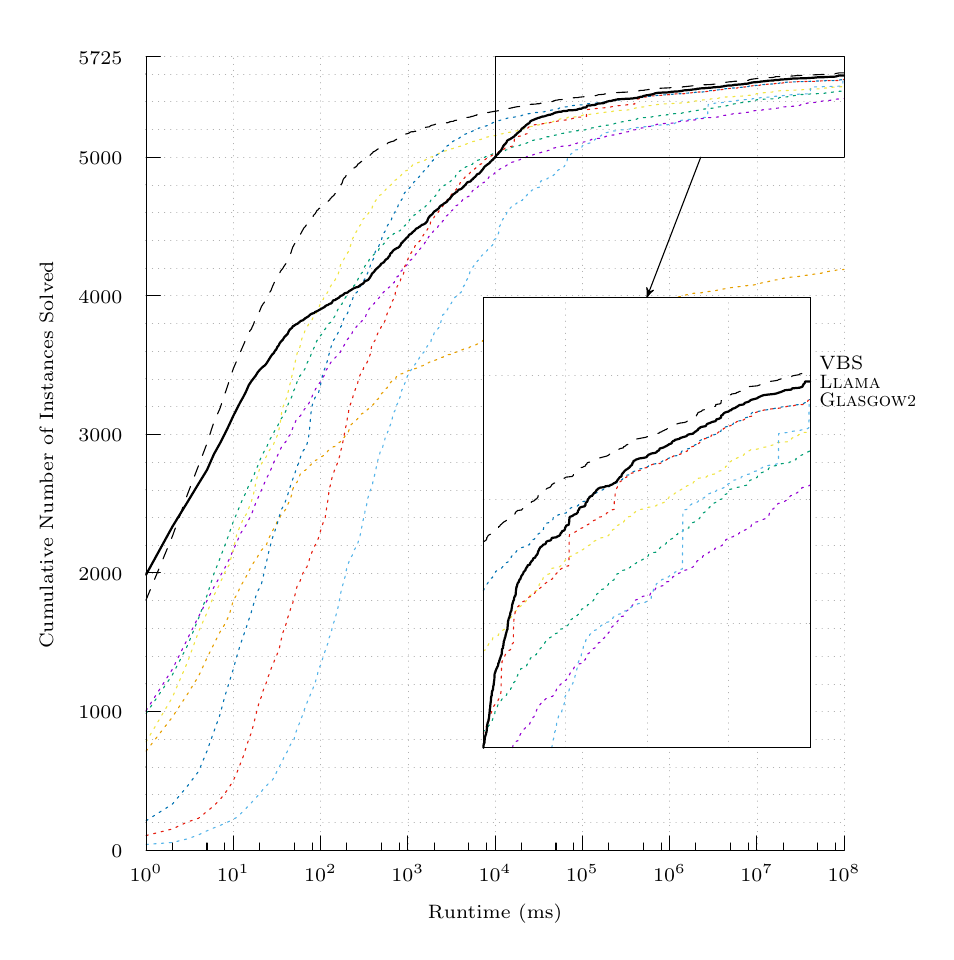
\begin{tikzpicture}[gnuplot]
%% generated with GNUPLOT 5.0p0 (Lua 5.2; terminal rev. 99, script rev. 100)
%% Wed 16 Dec 2015 18:50:09 GMT
\tikzset{every node/.append style={font={\scriptsize}}}
\path (0.000,0.000) rectangle (10.922,11.430);
\gpcolor{color=gp lt color axes}
\gpsetlinetype{gp lt axes}
\gpsetdashtype{gp dt axes}
\gpsetlinewidth{0.50}
\draw[gp path] (1.504,11.061)--(10.368,11.061);
\gpcolor{color=gp lt color border}
\gpsetlinetype{gp lt border}
\gpsetdashtype{gp dt solid}
\gpsetlinewidth{1.00}
\draw[gp path] (1.504,11.061)--(1.684,11.061);
\node[gp node right] at (1.320,11.061) {$5725$};
\gpcolor{color=gp lt color axes}
\gpsetlinetype{gp lt axes}
\gpsetdashtype{gp dt axes}
\gpsetlinewidth{0.50}
\draw[gp path] (1.504,0.985)--(10.368,0.985);
\gpcolor{color=gp lt color border}
\gpsetlinetype{gp lt border}
\gpsetdashtype{gp dt solid}
\gpsetlinewidth{1.00}
\draw[gp path] (1.504,0.985)--(1.684,0.985);
\node[gp node right] at (1.320,0.985) {$0$};
\gpcolor{color=gp lt color axes}
\gpsetlinetype{gp lt axes}
\gpsetdashtype{gp dt axes}
\gpsetlinewidth{0.50}
\draw[gp path] (1.504,1.337)--(10.368,1.337);
\gpcolor{color=gp lt color border}
\gpsetlinetype{gp lt border}
\gpsetdashtype{gp dt solid}
\gpsetlinewidth{1.00}
\draw[gp path] (1.504,1.337)--(1.505,1.337);
\gpcolor{color=gp lt color axes}
\gpsetlinetype{gp lt axes}
\gpsetdashtype{gp dt axes}
\gpsetlinewidth{0.50}
\draw[gp path] (1.504,1.689)--(10.368,1.689);
\gpcolor{color=gp lt color border}
\gpsetlinetype{gp lt border}
\gpsetdashtype{gp dt solid}
\gpsetlinewidth{1.00}
\draw[gp path] (1.504,1.689)--(1.505,1.689);
\gpcolor{color=gp lt color axes}
\gpsetlinetype{gp lt axes}
\gpsetdashtype{gp dt axes}
\gpsetlinewidth{0.50}
\draw[gp path] (1.504,2.041)--(10.368,2.041);
\gpcolor{color=gp lt color border}
\gpsetlinetype{gp lt border}
\gpsetdashtype{gp dt solid}
\gpsetlinewidth{1.00}
\draw[gp path] (1.504,2.041)--(1.505,2.041);
\gpcolor{color=gp lt color axes}
\gpsetlinetype{gp lt axes}
\gpsetdashtype{gp dt axes}
\gpsetlinewidth{0.50}
\draw[gp path] (1.504,2.393)--(10.368,2.393);
\gpcolor{color=gp lt color border}
\gpsetlinetype{gp lt border}
\gpsetdashtype{gp dt solid}
\gpsetlinewidth{1.00}
\draw[gp path] (1.504,2.393)--(1.505,2.393);
\gpcolor{color=gp lt color axes}
\gpsetlinetype{gp lt axes}
\gpsetdashtype{gp dt axes}
\gpsetlinewidth{0.50}
\draw[gp path] (1.504,2.745)--(10.368,2.745);
\gpcolor{color=gp lt color border}
\gpsetlinetype{gp lt border}
\gpsetdashtype{gp dt solid}
\gpsetlinewidth{1.00}
\draw[gp path] (1.504,2.745)--(1.684,2.745);
\node[gp node right] at (1.320,2.745) {$1000$};
\gpcolor{color=gp lt color axes}
\gpsetlinetype{gp lt axes}
\gpsetdashtype{gp dt axes}
\gpsetlinewidth{0.50}
\draw[gp path] (1.504,3.097)--(10.368,3.097);
\gpcolor{color=gp lt color border}
\gpsetlinetype{gp lt border}
\gpsetdashtype{gp dt solid}
\gpsetlinewidth{1.00}
\draw[gp path] (1.504,3.097)--(1.505,3.097);
\gpcolor{color=gp lt color axes}
\gpsetlinetype{gp lt axes}
\gpsetdashtype{gp dt axes}
\gpsetlinewidth{0.50}
\draw[gp path] (1.504,3.449)--(10.368,3.449);
\gpcolor{color=gp lt color border}
\gpsetlinetype{gp lt border}
\gpsetdashtype{gp dt solid}
\gpsetlinewidth{1.00}
\draw[gp path] (1.504,3.449)--(1.505,3.449);
\gpcolor{color=gp lt color axes}
\gpsetlinetype{gp lt axes}
\gpsetdashtype{gp dt axes}
\gpsetlinewidth{0.50}
\draw[gp path] (1.504,3.801)--(10.368,3.801);
\gpcolor{color=gp lt color border}
\gpsetlinetype{gp lt border}
\gpsetdashtype{gp dt solid}
\gpsetlinewidth{1.00}
\draw[gp path] (1.504,3.801)--(1.505,3.801);
\gpcolor{color=gp lt color axes}
\gpsetlinetype{gp lt axes}
\gpsetdashtype{gp dt axes}
\gpsetlinewidth{0.50}
\draw[gp path] (1.504,4.153)--(10.368,4.153);
\gpcolor{color=gp lt color border}
\gpsetlinetype{gp lt border}
\gpsetdashtype{gp dt solid}
\gpsetlinewidth{1.00}
\draw[gp path] (1.504,4.153)--(1.505,4.153);
\gpcolor{color=gp lt color axes}
\gpsetlinetype{gp lt axes}
\gpsetdashtype{gp dt axes}
\gpsetlinewidth{0.50}
\draw[gp path] (1.504,4.505)--(10.368,4.505);
\gpcolor{color=gp lt color border}
\gpsetlinetype{gp lt border}
\gpsetdashtype{gp dt solid}
\gpsetlinewidth{1.00}
\draw[gp path] (1.504,4.505)--(1.684,4.505);
\node[gp node right] at (1.320,4.505) {$2000$};
\gpcolor{color=gp lt color axes}
\gpsetlinetype{gp lt axes}
\gpsetdashtype{gp dt axes}
\gpsetlinewidth{0.50}
\draw[gp path] (1.504,4.857)--(10.368,4.857);
\gpcolor{color=gp lt color border}
\gpsetlinetype{gp lt border}
\gpsetdashtype{gp dt solid}
\gpsetlinewidth{1.00}
\draw[gp path] (1.504,4.857)--(1.505,4.857);
\gpcolor{color=gp lt color axes}
\gpsetlinetype{gp lt axes}
\gpsetdashtype{gp dt axes}
\gpsetlinewidth{0.50}
\draw[gp path] (1.504,5.209)--(10.368,5.209);
\gpcolor{color=gp lt color border}
\gpsetlinetype{gp lt border}
\gpsetdashtype{gp dt solid}
\gpsetlinewidth{1.00}
\draw[gp path] (1.504,5.209)--(1.505,5.209);
\gpcolor{color=gp lt color axes}
\gpsetlinetype{gp lt axes}
\gpsetdashtype{gp dt axes}
\gpsetlinewidth{0.50}
\draw[gp path] (1.504,5.561)--(10.368,5.561);
\gpcolor{color=gp lt color border}
\gpsetlinetype{gp lt border}
\gpsetdashtype{gp dt solid}
\gpsetlinewidth{1.00}
\draw[gp path] (1.504,5.561)--(1.505,5.561);
\gpcolor{color=gp lt color axes}
\gpsetlinetype{gp lt axes}
\gpsetdashtype{gp dt axes}
\gpsetlinewidth{0.50}
\draw[gp path] (1.504,5.913)--(10.368,5.913);
\gpcolor{color=gp lt color border}
\gpsetlinetype{gp lt border}
\gpsetdashtype{gp dt solid}
\gpsetlinewidth{1.00}
\draw[gp path] (1.504,5.913)--(1.505,5.913);
\gpcolor{color=gp lt color axes}
\gpsetlinetype{gp lt axes}
\gpsetdashtype{gp dt axes}
\gpsetlinewidth{0.50}
\draw[gp path] (1.504,6.265)--(10.368,6.265);
\gpcolor{color=gp lt color border}
\gpsetlinetype{gp lt border}
\gpsetdashtype{gp dt solid}
\gpsetlinewidth{1.00}
\draw[gp path] (1.504,6.265)--(1.684,6.265);
\node[gp node right] at (1.320,6.265) {$3000$};
\gpcolor{color=gp lt color axes}
\gpsetlinetype{gp lt axes}
\gpsetdashtype{gp dt axes}
\gpsetlinewidth{0.50}
\draw[gp path] (1.504,6.617)--(10.368,6.617);
\gpcolor{color=gp lt color border}
\gpsetlinetype{gp lt border}
\gpsetdashtype{gp dt solid}
\gpsetlinewidth{1.00}
\draw[gp path] (1.504,6.617)--(1.505,6.617);
\gpcolor{color=gp lt color axes}
\gpsetlinetype{gp lt axes}
\gpsetdashtype{gp dt axes}
\gpsetlinewidth{0.50}
\draw[gp path] (1.504,6.969)--(10.368,6.969);
\gpcolor{color=gp lt color border}
\gpsetlinetype{gp lt border}
\gpsetdashtype{gp dt solid}
\gpsetlinewidth{1.00}
\draw[gp path] (1.504,6.969)--(1.505,6.969);
\gpcolor{color=gp lt color axes}
\gpsetlinetype{gp lt axes}
\gpsetdashtype{gp dt axes}
\gpsetlinewidth{0.50}
\draw[gp path] (1.504,7.321)--(10.368,7.321);
\gpcolor{color=gp lt color border}
\gpsetlinetype{gp lt border}
\gpsetdashtype{gp dt solid}
\gpsetlinewidth{1.00}
\draw[gp path] (1.504,7.321)--(1.505,7.321);
\gpcolor{color=gp lt color axes}
\gpsetlinetype{gp lt axes}
\gpsetdashtype{gp dt axes}
\gpsetlinewidth{0.50}
\draw[gp path] (1.504,7.673)--(10.368,7.673);
\gpcolor{color=gp lt color border}
\gpsetlinetype{gp lt border}
\gpsetdashtype{gp dt solid}
\gpsetlinewidth{1.00}
\draw[gp path] (1.504,7.673)--(1.505,7.673);
\gpcolor{color=gp lt color axes}
\gpsetlinetype{gp lt axes}
\gpsetdashtype{gp dt axes}
\gpsetlinewidth{0.50}
\draw[gp path] (1.504,8.025)--(10.368,8.025);
\gpcolor{color=gp lt color border}
\gpsetlinetype{gp lt border}
\gpsetdashtype{gp dt solid}
\gpsetlinewidth{1.00}
\draw[gp path] (1.504,8.025)--(1.684,8.025);
\node[gp node right] at (1.320,8.025) {$4000$};
\gpcolor{color=gp lt color axes}
\gpsetlinetype{gp lt axes}
\gpsetdashtype{gp dt axes}
\gpsetlinewidth{0.50}
\draw[gp path] (1.504,8.377)--(10.368,8.377);
\gpcolor{color=gp lt color border}
\gpsetlinetype{gp lt border}
\gpsetdashtype{gp dt solid}
\gpsetlinewidth{1.00}
\draw[gp path] (1.504,8.377)--(1.505,8.377);
\gpcolor{color=gp lt color axes}
\gpsetlinetype{gp lt axes}
\gpsetdashtype{gp dt axes}
\gpsetlinewidth{0.50}
\draw[gp path] (1.504,8.729)--(10.368,8.729);
\gpcolor{color=gp lt color border}
\gpsetlinetype{gp lt border}
\gpsetdashtype{gp dt solid}
\gpsetlinewidth{1.00}
\draw[gp path] (1.504,8.729)--(1.505,8.729);
\gpcolor{color=gp lt color axes}
\gpsetlinetype{gp lt axes}
\gpsetdashtype{gp dt axes}
\gpsetlinewidth{0.50}
\draw[gp path] (1.504,9.081)--(10.368,9.081);
\gpcolor{color=gp lt color border}
\gpsetlinetype{gp lt border}
\gpsetdashtype{gp dt solid}
\gpsetlinewidth{1.00}
\draw[gp path] (1.504,9.081)--(1.505,9.081);
\gpcolor{color=gp lt color axes}
\gpsetlinetype{gp lt axes}
\gpsetdashtype{gp dt axes}
\gpsetlinewidth{0.50}
\draw[gp path] (1.504,9.433)--(10.368,9.433);
\gpcolor{color=gp lt color border}
\gpsetlinetype{gp lt border}
\gpsetdashtype{gp dt solid}
\gpsetlinewidth{1.00}
\draw[gp path] (1.504,9.433)--(1.505,9.433);
\gpcolor{color=gp lt color axes}
\gpsetlinetype{gp lt axes}
\gpsetdashtype{gp dt axes}
\gpsetlinewidth{0.50}
\draw[gp path] (1.504,9.785)--(10.368,9.785);
\gpcolor{color=gp lt color border}
\gpsetlinetype{gp lt border}
\gpsetdashtype{gp dt solid}
\gpsetlinewidth{1.00}
\draw[gp path] (1.504,9.785)--(1.684,9.785);
\node[gp node right] at (1.320,9.785) {$5000$};
\gpcolor{color=gp lt color axes}
\gpsetlinetype{gp lt axes}
\gpsetdashtype{gp dt axes}
\gpsetlinewidth{0.50}
\draw[gp path] (1.504,10.137)--(10.368,10.137);
\gpcolor{color=gp lt color border}
\gpsetlinetype{gp lt border}
\gpsetdashtype{gp dt solid}
\gpsetlinewidth{1.00}
\draw[gp path] (1.504,10.137)--(1.505,10.137);
\gpcolor{color=gp lt color axes}
\gpsetlinetype{gp lt axes}
\gpsetdashtype{gp dt axes}
\gpsetlinewidth{0.50}
\draw[gp path] (1.504,10.489)--(10.368,10.489);
\gpcolor{color=gp lt color border}
\gpsetlinetype{gp lt border}
\gpsetdashtype{gp dt solid}
\gpsetlinewidth{1.00}
\draw[gp path] (1.504,10.489)--(1.505,10.489);
\gpcolor{color=gp lt color axes}
\gpsetlinetype{gp lt axes}
\gpsetdashtype{gp dt axes}
\gpsetlinewidth{0.50}
\draw[gp path] (1.504,10.841)--(10.368,10.841);
\gpcolor{color=gp lt color border}
\gpsetlinetype{gp lt border}
\gpsetdashtype{gp dt solid}
\gpsetlinewidth{1.00}
\draw[gp path] (1.504,10.841)--(1.505,10.841);
\gpcolor{color=gp lt color axes}
\gpsetlinetype{gp lt axes}
\gpsetdashtype{gp dt axes}
\gpsetlinewidth{0.50}
\draw[gp path] (1.504,0.985)--(1.504,11.061);
\gpcolor{color=gp lt color border}
\gpsetlinetype{gp lt border}
\gpsetdashtype{gp dt solid}
\gpsetlinewidth{1.00}
\draw[gp path] (1.504,0.985)--(1.504,1.165);
\node[gp node center] at (1.504,0.677) {$10^{0}$};
\draw[gp path] (1.838,0.985)--(1.838,1.075);
\draw[gp path] (2.278,0.985)--(2.278,1.075);
\draw[gp path] (2.505,0.985)--(2.505,1.075);
\gpcolor{color=gp lt color axes}
\gpsetlinetype{gp lt axes}
\gpsetdashtype{gp dt axes}
\gpsetlinewidth{0.50}
\draw[gp path] (2.612,0.985)--(2.612,11.061);
\gpcolor{color=gp lt color border}
\gpsetlinetype{gp lt border}
\gpsetdashtype{gp dt solid}
\gpsetlinewidth{1.00}
\draw[gp path] (2.612,0.985)--(2.612,1.165);
\node[gp node center] at (2.612,0.677) {$10^{1}$};
\draw[gp path] (2.946,0.985)--(2.946,1.075);
\draw[gp path] (3.386,0.985)--(3.386,1.075);
\draw[gp path] (3.613,0.985)--(3.613,1.075);
\gpcolor{color=gp lt color axes}
\gpsetlinetype{gp lt axes}
\gpsetdashtype{gp dt axes}
\gpsetlinewidth{0.50}
\draw[gp path] (3.720,0.985)--(3.720,11.061);
\gpcolor{color=gp lt color border}
\gpsetlinetype{gp lt border}
\gpsetdashtype{gp dt solid}
\gpsetlinewidth{1.00}
\draw[gp path] (3.720,0.985)--(3.720,1.165);
\node[gp node center] at (3.720,0.677) {$10^{2}$};
\draw[gp path] (4.054,0.985)--(4.054,1.075);
\draw[gp path] (4.494,0.985)--(4.494,1.075);
\draw[gp path] (4.721,0.985)--(4.721,1.075);
\gpcolor{color=gp lt color axes}
\gpsetlinetype{gp lt axes}
\gpsetdashtype{gp dt axes}
\gpsetlinewidth{0.50}
\draw[gp path] (4.828,0.985)--(4.828,11.061);
\gpcolor{color=gp lt color border}
\gpsetlinetype{gp lt border}
\gpsetdashtype{gp dt solid}
\gpsetlinewidth{1.00}
\draw[gp path] (4.828,0.985)--(4.828,1.165);
\node[gp node center] at (4.828,0.677) {$10^{3}$};
\draw[gp path] (5.162,0.985)--(5.162,1.075);
\draw[gp path] (5.602,0.985)--(5.602,1.075);
\draw[gp path] (5.829,0.985)--(5.829,1.075);
\gpcolor{color=gp lt color axes}
\gpsetlinetype{gp lt axes}
\gpsetdashtype{gp dt axes}
\gpsetlinewidth{0.50}
\draw[gp path] (5.936,0.985)--(5.936,11.061);
\gpcolor{color=gp lt color border}
\gpsetlinetype{gp lt border}
\gpsetdashtype{gp dt solid}
\gpsetlinewidth{1.00}
\draw[gp path] (5.936,0.985)--(5.936,1.165);
\node[gp node center] at (5.936,0.677) {$10^{4}$};
\draw[gp path] (6.270,0.985)--(6.270,1.075);
\draw[gp path] (6.710,0.985)--(6.710,1.075);
\draw[gp path] (6.937,0.985)--(6.937,1.075);
\gpcolor{color=gp lt color axes}
\gpsetlinetype{gp lt axes}
\gpsetdashtype{gp dt axes}
\gpsetlinewidth{0.50}
\draw[gp path] (7.044,0.985)--(7.044,11.061);
\gpcolor{color=gp lt color border}
\gpsetlinetype{gp lt border}
\gpsetdashtype{gp dt solid}
\gpsetlinewidth{1.00}
\draw[gp path] (7.044,0.985)--(7.044,1.165);
\node[gp node center] at (7.044,0.677) {$10^{5}$};
\draw[gp path] (7.378,0.985)--(7.378,1.075);
\draw[gp path] (7.818,0.985)--(7.818,1.075);
\draw[gp path] (8.045,0.985)--(8.045,1.075);
\gpcolor{color=gp lt color axes}
\gpsetlinetype{gp lt axes}
\gpsetdashtype{gp dt axes}
\gpsetlinewidth{0.50}
\draw[gp path] (8.152,0.985)--(8.152,11.061);
\gpcolor{color=gp lt color border}
\gpsetlinetype{gp lt border}
\gpsetdashtype{gp dt solid}
\gpsetlinewidth{1.00}
\draw[gp path] (8.152,0.985)--(8.152,1.165);
\node[gp node center] at (8.152,0.677) {$10^{6}$};
\draw[gp path] (8.486,0.985)--(8.486,1.075);
\draw[gp path] (8.926,0.985)--(8.926,1.075);
\draw[gp path] (9.153,0.985)--(9.153,1.075);
\gpcolor{color=gp lt color axes}
\gpsetlinetype{gp lt axes}
\gpsetdashtype{gp dt axes}
\gpsetlinewidth{0.50}
\draw[gp path] (9.260,0.985)--(9.260,11.061);
\gpcolor{color=gp lt color border}
\gpsetlinetype{gp lt border}
\gpsetdashtype{gp dt solid}
\gpsetlinewidth{1.00}
\draw[gp path] (9.260,0.985)--(9.260,1.165);
\node[gp node center] at (9.260,0.677) {$10^{7}$};
\draw[gp path] (9.594,0.985)--(9.594,1.075);
\draw[gp path] (10.034,0.985)--(10.034,1.075);
\draw[gp path] (10.261,0.985)--(10.261,1.075);
\gpcolor{color=gp lt color axes}
\gpsetlinetype{gp lt axes}
\gpsetdashtype{gp dt axes}
\gpsetlinewidth{0.50}
\draw[gp path] (10.368,0.985)--(10.368,11.061);
\gpcolor{color=gp lt color border}
\gpsetlinetype{gp lt border}
\gpsetdashtype{gp dt solid}
\gpsetlinewidth{1.00}
\draw[gp path] (10.368,0.985)--(10.368,1.165);
\node[gp node center] at (10.368,0.677) {$10^{8}$};
\draw[gp path] (1.504,11.061)--(1.504,0.985)--(10.368,0.985);
\node[gp node center,rotate=-270] at (0.246,6.023) {Cumulative Number of Instances Solved};
\node[gp node center] at (5.936,0.215) {Runtime (ms)};
\gpcolor{rgb color={0.580,0.000,0.827}}
\gpsetdashtype{dash pattern=on 2.00*\gpdashlength off 5.00*\gpdashlength }
\draw[gp path] (1.504,2.757)--(1.838,3.282)--(2.033,3.676)--(2.171,3.952)--(2.278,4.155)%
  --(2.366,4.327)--(2.440,4.457)--(2.505,4.570)--(2.561,4.683)--(2.612,4.799)--(2.658,4.899)%
  --(2.700,5.000)--(2.738,5.059)--(2.774,5.116)--(2.807,5.181)--(2.838,5.235)--(2.867,5.316)%
  --(2.895,5.390)--(2.921,5.448)--(2.946,5.506)--(2.969,5.556)--(2.991,5.607)--(3.013,5.661)%
  --(3.033,5.705)--(3.053,5.744)--(3.072,5.786)--(3.090,5.821)--(3.107,5.864)--(3.124,5.908)%
  --(3.141,5.939)--(3.156,5.966)--(3.172,5.994)--(3.187,6.027)--(3.201,6.052)--(3.215,6.087)%
  --(3.228,6.112)--(3.242,6.128)--(3.254,6.144)--(3.267,6.161)--(3.279,6.173)--(3.291,6.188)%
  --(3.303,6.219)--(3.314,6.237)--(3.325,6.253)--(3.336,6.263)--(3.346,6.276)--(3.357,6.318)%
  --(3.367,6.349)--(3.377,6.371)--(3.386,6.390)--(3.396,6.413)--(3.405,6.436)--(3.414,6.455)%
  --(3.423,6.462)--(3.432,6.478)--(3.441,6.480)--(3.450,6.489)--(3.458,6.496)--(3.466,6.504)%
  --(3.474,6.517)--(3.482,6.525)--(3.490,6.534)--(3.498,6.547)--(3.505,6.562)--(3.513,6.584)%
  --(3.520,6.589)--(3.527,6.596)--(3.534,6.610)--(3.541,6.617)--(3.548,6.629)--(3.555,6.636)%
  --(3.562,6.647)--(3.569,6.657)--(3.575,6.665)--(3.582,6.689)--(3.588,6.703)--(3.594,6.712)%
  --(3.600,6.723)--(3.607,6.737)--(3.613,6.747)--(3.619,6.765)--(3.625,6.774)--(3.630,6.789)%
  --(3.636,6.805)--(3.642,6.816)--(3.647,6.823)--(3.653,6.833)--(3.658,6.844)--(3.664,6.853)%
  --(3.669,6.860)--(3.675,6.869)--(3.680,6.877)--(3.685,6.881)--(3.690,6.899)--(3.695,6.906)%
  --(3.700,6.911)--(3.705,6.914)--(3.710,6.923)--(3.715,6.927)--(3.720,6.932)--(3.725,6.936)%
  --(3.730,6.943)--(3.734,6.950)--(3.739,6.971)--(3.743,6.980)--(3.748,6.987)--(3.753,6.992)%
  --(3.757,7.001)--(3.761,7.004)--(3.766,7.013)--(3.770,7.024)--(3.775,7.043)--(3.779,7.046)%
  --(3.783,7.059)--(3.787,7.071)--(3.791,7.083)--(3.796,7.089)--(3.804,7.099)--(3.808,7.106)%
  --(3.812,7.115)--(3.816,7.124)--(3.820,7.126)--(3.824,7.131)--(3.827,7.140)--(3.831,7.149)%
  --(3.835,7.150)--(3.839,7.159)--(3.843,7.166)--(3.846,7.173)--(3.850,7.177)--(3.854,7.185)%
  --(3.857,7.194)--(3.861,7.196)--(3.864,7.200)--(3.868,7.201)--(3.871,7.205)--(3.875,7.207)%
  --(3.878,7.208)--(3.882,7.217)--(3.885,7.222)--(3.892,7.224)--(3.895,7.229)--(3.899,7.233)%
  --(3.905,7.237)--(3.909,7.244)--(3.915,7.247)--(3.918,7.252)--(3.921,7.258)--(3.925,7.263)%
  --(3.928,7.266)--(3.931,7.268)--(3.934,7.275)--(3.940,7.281)--(3.943,7.286)--(3.949,7.291)%
  --(3.952,7.293)--(3.955,7.295)--(3.958,7.298)--(3.961,7.300)--(3.964,7.303)--(3.967,7.305)%
  --(3.970,7.310)--(3.972,7.317)--(3.975,7.325)--(3.978,7.326)--(3.981,7.328)--(3.984,7.332)%
  --(3.987,7.339)--(3.989,7.347)--(3.992,7.354)--(3.995,7.358)--(4.000,7.361)--(4.003,7.370)%
  --(4.006,7.376)--(4.008,7.383)--(4.011,7.386)--(4.013,7.388)--(4.016,7.390)--(4.019,7.393)%
  --(4.021,7.400)--(4.024,7.404)--(4.026,7.411)--(4.029,7.414)--(4.031,7.420)--(4.034,7.423)%
  --(4.036,7.427)--(4.039,7.430)--(4.041,7.439)--(4.044,7.442)--(4.049,7.448)--(4.051,7.453)%
  --(4.054,7.458)--(4.056,7.465)--(4.058,7.469)--(4.061,7.471)--(4.063,7.474)--(4.068,7.478)%
  --(4.070,7.481)--(4.072,7.483)--(4.075,7.485)--(4.077,7.492)--(4.079,7.493)--(4.082,7.499)%
  --(4.084,7.501)--(4.086,7.504)--(4.091,7.506)--(4.093,7.509)--(4.095,7.511)--(4.097,7.513)%
  --(4.099,7.515)--(4.102,7.522)--(4.106,7.523)--(4.108,7.525)--(4.110,7.532)--(4.112,7.539)%
  --(4.114,7.543)--(4.119,7.548)--(4.121,7.555)--(4.123,7.560)--(4.125,7.566)--(4.127,7.573)%
  --(4.129,7.576)--(4.131,7.581)--(4.133,7.583)--(4.135,7.587)--(4.139,7.590)--(4.141,7.594)%
  --(4.145,7.596)--(4.147,7.599)--(4.149,7.603)--(4.155,7.610)--(4.157,7.611)--(4.159,7.615)%
  --(4.161,7.617)--(4.163,7.620)--(4.165,7.622)--(4.169,7.624)--(4.170,7.625)--(4.172,7.629)%
  --(4.174,7.633)--(4.176,7.634)--(4.180,7.640)--(4.183,7.641)--(4.185,7.645)--(4.187,7.647)%
  --(4.189,7.648)--(4.191,7.650)--(4.193,7.654)--(4.194,7.657)--(4.196,7.664)--(4.198,7.666)%
  --(4.200,7.668)--(4.207,7.671)--(4.210,7.675)--(4.212,7.678)--(4.214,7.680)--(4.215,7.682)%
  --(4.219,7.684)--(4.221,7.685)--(4.222,7.687)--(4.224,7.689)--(4.227,7.691)--(4.232,7.692)%
  --(4.234,7.694)--(4.236,7.698)--(4.239,7.699)--(4.241,7.703)--(4.242,7.705)--(4.245,7.706)%
  --(4.250,7.708)--(4.252,7.712)--(4.253,7.715)--(4.255,7.721)--(4.257,7.722)--(4.258,7.724)%
  --(4.260,7.726)--(4.261,7.731)--(4.263,7.733)--(4.264,7.735)--(4.266,7.740)--(4.271,7.742)%
  --(4.272,7.743)--(4.274,7.745)--(4.275,7.749)--(4.277,7.750)--(4.278,7.752)--(4.280,7.754)%
  --(4.283,7.757)--(4.289,7.759)--(4.292,7.765)--(4.293,7.766)--(4.295,7.768)--(4.296,7.777)%
  --(4.297,7.780)--(4.299,7.784)--(4.302,7.789)--(4.303,7.791)--(4.305,7.794)--(4.306,7.798)%
  --(4.307,7.801)--(4.309,7.805)--(4.310,7.809)--(4.312,7.810)--(4.315,7.812)--(4.316,7.814)%
  --(4.317,7.816)--(4.319,7.819)--(4.320,7.823)--(4.321,7.828)--(4.323,7.831)--(4.324,7.833)%
  --(4.326,7.838)--(4.327,7.840)--(4.328,7.844)--(4.331,7.849)--(4.332,7.851)--(4.334,7.853)%
  --(4.335,7.854)--(4.336,7.858)--(4.338,7.861)--(4.339,7.863)--(4.340,7.865)--(4.343,7.867)%
  --(4.346,7.870)--(4.347,7.875)--(4.348,7.877)--(4.351,7.879)--(4.353,7.881)--(4.355,7.882)%
  --(4.359,7.888)--(4.362,7.889)--(4.367,7.891)--(4.369,7.895)--(4.370,7.900)--(4.371,7.902)%
  --(4.372,7.904)--(4.375,7.905)--(4.379,7.907)--(4.381,7.911)--(4.382,7.914)--(4.387,7.916)%
  --(4.388,7.918)--(4.389,7.919)--(4.394,7.921)--(4.397,7.923)--(4.398,7.925)--(4.402,7.926)%
  --(4.404,7.932)--(4.405,7.933)--(4.406,7.935)--(4.407,7.937)--(4.409,7.941)--(4.411,7.942)%
  --(4.412,7.946)--(4.414,7.948)--(4.415,7.951)--(4.417,7.953)--(4.420,7.955)--(4.421,7.956)%
  --(4.423,7.958)--(4.430,7.962)--(4.432,7.963)--(4.437,7.965)--(4.441,7.969)--(4.443,7.972)%
  --(4.444,7.974)--(4.445,7.976)--(4.447,7.977)--(4.448,7.983)--(4.450,7.985)--(4.452,7.988)%
  --(4.453,7.990)--(4.454,7.992)--(4.459,7.995)--(4.460,7.997)--(4.463,7.999)--(4.465,8.000)%
  --(4.466,8.002)--(4.467,8.004)--(4.468,8.006)--(4.469,8.007)--(4.470,8.011)--(4.471,8.014)%
  --(4.472,8.018)--(4.473,8.020)--(4.475,8.023)--(4.481,8.025)--(4.482,8.027)--(4.483,8.030)%
  --(4.485,8.032)--(4.486,8.036)--(4.491,8.037)--(4.492,8.039)--(4.496,8.043)--(4.498,8.044)%
  --(4.499,8.046)--(4.501,8.048)--(4.502,8.050)--(4.503,8.051)--(4.504,8.053)--(4.505,8.055)%
  --(4.507,8.057)--(4.508,8.058)--(4.509,8.060)--(4.511,8.062)--(4.515,8.065)--(4.518,8.067)%
  --(4.519,8.069)--(4.523,8.074)--(4.527,8.076)--(4.529,8.078)--(4.530,8.080)--(4.531,8.083)%
  --(4.534,8.085)--(4.542,8.087)--(4.544,8.090)--(4.547,8.092)--(4.551,8.094)--(4.557,8.097)%
  --(4.558,8.101)--(4.560,8.102)--(4.561,8.104)--(4.563,8.106)--(4.564,8.108)--(4.567,8.109)%
  --(4.569,8.113)--(4.575,8.115)--(4.576,8.117)--(4.577,8.118)--(4.578,8.120)--(4.580,8.124)%
  --(4.581,8.125)--(4.582,8.127)--(4.586,8.129)--(4.587,8.131)--(4.590,8.132)--(4.592,8.134)%
  --(4.593,8.138)--(4.599,8.139)--(4.600,8.141)--(4.603,8.143)--(4.604,8.150)--(4.606,8.152)%
  --(4.606,8.153)--(4.609,8.155)--(4.611,8.157)--(4.620,8.159)--(4.621,8.161)--(4.623,8.162)%
  --(4.624,8.164)--(4.626,8.166)--(4.627,8.168)--(4.628,8.171)--(4.635,8.173)--(4.635,8.175)%
  --(4.636,8.178)--(4.637,8.180)--(4.639,8.182)--(4.641,8.183)--(4.642,8.185)--(4.644,8.187)%
  --(4.648,8.189)--(4.649,8.190)--(4.650,8.192)--(4.653,8.194)--(4.656,8.196)--(4.657,8.201)%
  --(4.658,8.205)--(4.658,8.206)--(4.660,8.208)--(4.661,8.210)--(4.663,8.212)--(4.664,8.213)%
  --(4.669,8.215)--(4.669,8.217)--(4.670,8.219)--(4.671,8.220)--(4.671,8.222)--(4.675,8.226)%
  --(4.677,8.227)--(4.677,8.231)--(4.678,8.233)--(4.679,8.234)--(4.679,8.236)--(4.682,8.238)%
  --(4.684,8.240)--(4.684,8.243)--(4.685,8.245)--(4.686,8.249)--(4.686,8.254)--(4.688,8.256)%
  --(4.690,8.257)--(4.691,8.263)--(4.691,8.268)--(4.693,8.270)--(4.693,8.271)--(4.704,8.273)%
  --(4.706,8.275)--(4.707,8.277)--(4.708,8.278)--(4.709,8.284)--(4.710,8.287)--(4.711,8.291)%
  --(4.713,8.293)--(4.719,8.294)--(4.720,8.296)--(4.721,8.298)--(4.722,8.300)--(4.723,8.301)%
  --(4.724,8.303)--(4.726,8.307)--(4.727,8.308)--(4.728,8.312)--(4.729,8.315)--(4.732,8.317)%
  --(4.733,8.319)--(4.733,8.321)--(4.734,8.324)--(4.735,8.328)--(4.737,8.333)--(4.738,8.337)%
  --(4.738,8.338)--(4.743,8.340)--(4.745,8.342)--(4.753,8.344)--(4.754,8.347)--(4.754,8.349)%
  --(4.757,8.354)--(4.762,8.356)--(4.763,8.359)--(4.764,8.361)--(4.766,8.363)--(4.767,8.365)%
  --(4.768,8.366)--(4.769,8.368)--(4.770,8.370)--(4.772,8.373)--(4.783,8.375)--(4.783,8.377)%
  --(4.784,8.379)--(4.789,8.381)--(4.789,8.382)--(4.790,8.384)--(4.792,8.386)--(4.794,8.388)%
  --(4.794,8.391)--(4.795,8.393)--(4.796,8.395)--(4.797,8.396)--(4.798,8.398)--(4.800,8.400)%
  --(4.801,8.402)--(4.804,8.403)--(4.807,8.407)--(4.809,8.409)--(4.810,8.410)--(4.812,8.412)%
  --(4.814,8.414)--(4.816,8.416)--(4.819,8.419)--(4.820,8.421)--(4.821,8.423)--(4.821,8.426)%
  --(4.822,8.428)--(4.823,8.430)--(4.823,8.432)--(4.826,8.433)--(4.827,8.435)--(4.829,8.437)%
  --(4.832,8.439)--(4.833,8.442)--(4.837,8.444)--(4.838,8.447)--(4.840,8.449)--(4.843,8.451)%
  --(4.848,8.453)--(4.849,8.454)--(4.850,8.456)--(4.851,8.458)--(4.851,8.461)--(4.851,8.463)%
  --(4.852,8.465)--(4.853,8.470)--(4.855,8.474)--(4.856,8.476)--(4.861,8.477)--(4.865,8.479)%
  --(4.868,8.481)--(4.869,8.483)--(4.869,8.484)--(4.873,8.486)--(4.876,8.488)--(4.882,8.490)%
  --(4.883,8.491)--(4.886,8.493)--(4.886,8.495)--(4.889,8.498)--(4.891,8.500)--(4.893,8.504)%
  --(4.893,8.505)--(4.894,8.507)--(4.896,8.509)--(4.897,8.511)--(4.897,8.513)--(4.901,8.514)%
  --(4.902,8.518)--(4.904,8.520)--(4.906,8.523)--(4.907,8.525)--(4.909,8.527)--(4.911,8.528)%
  --(4.913,8.532)--(4.913,8.534)--(4.914,8.535)--(4.915,8.537)--(4.917,8.539)--(4.921,8.541)%
  --(4.921,8.542)--(4.925,8.546)--(4.926,8.548)--(4.926,8.549)--(4.927,8.551)--(4.927,8.553)%
  --(4.928,8.555)--(4.931,8.557)--(4.932,8.558)--(4.933,8.560)--(4.938,8.562)--(4.939,8.564)%
  --(4.940,8.567)--(4.941,8.569)--(4.943,8.571)--(4.944,8.572)--(4.950,8.574)--(4.950,8.576)%
  --(4.954,8.579)--(4.955,8.581)--(4.955,8.583)--(4.958,8.585)--(4.958,8.586)--(4.960,8.588)%
  --(4.963,8.590)--(4.964,8.592)--(4.966,8.593)--(4.971,8.595)--(4.972,8.597)--(4.973,8.599)%
  --(4.973,8.601)--(4.974,8.602)--(4.976,8.606)--(4.976,8.608)--(4.977,8.611)--(4.979,8.613)%
  --(4.980,8.615)--(4.981,8.616)--(4.982,8.618)--(4.983,8.620)--(4.984,8.622)--(4.986,8.623)%
  --(4.986,8.625)--(4.987,8.627)--(4.989,8.629)--(4.991,8.630)--(4.994,8.632)--(4.996,8.634)%
  --(4.998,8.636)--(5.000,8.637)--(5.004,8.639)--(5.005,8.641)--(5.005,8.643)--(5.007,8.645)%
  --(5.011,8.648)--(5.012,8.650)--(5.016,8.652)--(5.019,8.653)--(5.019,8.655)--(5.020,8.657)%
  --(5.022,8.659)--(5.023,8.660)--(5.025,8.664)--(5.026,8.666)--(5.026,8.667)--(5.030,8.673)%
  --(5.031,8.674)--(5.032,8.676)--(5.034,8.680)--(5.036,8.683)--(5.037,8.685)--(5.039,8.687)%
  --(5.039,8.689)--(5.040,8.690)--(5.040,8.692)--(5.041,8.694)--(5.043,8.699)--(5.045,8.701)%
  --(5.048,8.703)--(5.049,8.704)--(5.051,8.706)--(5.053,8.708)--(5.054,8.710)--(5.054,8.711)%
  --(5.057,8.713)--(5.058,8.717)--(5.059,8.718)--(5.059,8.720)--(5.060,8.722)--(5.060,8.724)%
  --(5.061,8.725)--(5.064,8.727)--(5.064,8.729)--(5.065,8.731)--(5.065,8.733)--(5.066,8.734)%
  --(5.067,8.738)--(5.067,8.740)--(5.069,8.741)--(5.069,8.743)--(5.071,8.745)--(5.078,8.747)%
  --(5.082,8.748)--(5.082,8.752)--(5.083,8.755)--(5.084,8.757)--(5.085,8.759)--(5.087,8.761)%
  --(5.087,8.762)--(5.088,8.764)--(5.088,8.766)--(5.088,8.768)--(5.090,8.769)--(5.092,8.771)%
  --(5.093,8.775)--(5.097,8.777)--(5.098,8.778)--(5.100,8.780)--(5.102,8.782)--(5.103,8.784)%
  --(5.103,8.785)--(5.104,8.787)--(5.106,8.789)--(5.106,8.791)--(5.111,8.792)--(5.115,8.794)%
  --(5.116,8.796)--(5.117,8.798)--(5.117,8.799)--(5.119,8.801)--(5.121,8.803)--(5.121,8.808)%
  --(5.122,8.810)--(5.122,8.812)--(5.125,8.813)--(5.130,8.817)--(5.131,8.819)--(5.131,8.821)%
  --(5.132,8.822)--(5.134,8.824)--(5.134,8.826)--(5.136,8.829)--(5.146,8.831)--(5.146,8.833)%
  --(5.147,8.836)--(5.147,8.838)--(5.148,8.840)--(5.149,8.842)--(5.149,8.843)--(5.154,8.845)%
  --(5.155,8.847)--(5.156,8.849)--(5.156,8.854)--(5.163,8.857)--(5.165,8.859)--(5.166,8.861)%
  --(5.168,8.863)--(5.171,8.866)--(5.174,8.868)--(5.177,8.870)--(5.178,8.872)--(5.181,8.873)%
  --(5.186,8.875)--(5.187,8.877)--(5.189,8.879)--(5.189,8.880)--(5.192,8.882)--(5.194,8.884)%
  --(5.197,8.886)--(5.199,8.887)--(5.201,8.889)--(5.203,8.891)--(5.204,8.893)--(5.206,8.894)%
  --(5.206,8.896)--(5.208,8.898)--(5.210,8.901)--(5.210,8.903)--(5.211,8.905)--(5.211,8.907)%
  --(5.214,8.910)--(5.217,8.914)--(5.225,8.916)--(5.226,8.917)--(5.226,8.919)--(5.227,8.921)%
  --(5.232,8.923)--(5.236,8.924)--(5.239,8.926)--(5.239,8.928)--(5.240,8.930)--(5.241,8.931)%
  --(5.245,8.933)--(5.246,8.935)--(5.250,8.937)--(5.251,8.940)--(5.251,8.942)--(5.255,8.944)%
  --(5.255,8.945)--(5.259,8.949)--(5.260,8.951)--(5.261,8.953)--(5.262,8.954)--(5.263,8.956)%
  --(5.263,8.958)--(5.264,8.960)--(5.265,8.963)--(5.265,8.965)--(5.267,8.967)--(5.268,8.968)%
  --(5.268,8.970)--(5.269,8.972)--(5.270,8.974)--(5.275,8.977)--(5.277,8.979)--(5.278,8.981)%
  --(5.281,8.982)--(5.282,8.984)--(5.283,8.986)--(5.284,8.988)--(5.286,8.989)--(5.289,8.991)%
  --(5.290,8.993)--(5.291,8.995)--(5.292,8.997)--(5.292,8.998)--(5.293,9.002)--(5.294,9.004)%
  --(5.294,9.005)--(5.294,9.007)--(5.294,9.009)--(5.296,9.011)--(5.297,9.012)--(5.298,9.014)%
  --(5.299,9.018)--(5.300,9.019)--(5.301,9.021)--(5.302,9.023)--(5.305,9.025)--(5.306,9.026)%
  --(5.308,9.028)--(5.310,9.030)--(5.312,9.032)--(5.312,9.033)--(5.314,9.035)--(5.315,9.037)%
  --(5.318,9.039)--(5.323,9.041)--(5.326,9.042)--(5.327,9.044)--(5.329,9.046)--(5.331,9.048)%
  --(5.332,9.049)--(5.333,9.051)--(5.338,9.053)--(5.338,9.055)--(5.339,9.056)--(5.340,9.058)%
  --(5.341,9.060)--(5.341,9.062)--(5.347,9.063)--(5.347,9.065)--(5.350,9.067)--(5.352,9.069)%
  --(5.352,9.070)--(5.353,9.072)--(5.353,9.074)--(5.354,9.076)--(5.355,9.077)--(5.361,9.079)%
  --(5.361,9.081)--(5.363,9.083)--(5.365,9.085)--(5.366,9.086)--(5.368,9.090)--(5.369,9.093)%
  --(5.372,9.097)--(5.374,9.099)--(5.378,9.100)--(5.379,9.102)--(5.384,9.104)--(5.385,9.106)%
  --(5.389,9.107)--(5.392,9.109)--(5.392,9.111)--(5.393,9.113)--(5.396,9.114)--(5.399,9.116)%
  --(5.400,9.118)--(5.400,9.120)--(5.402,9.121)--(5.403,9.123)--(5.404,9.125)--(5.405,9.127)%
  --(5.405,9.129)--(5.409,9.132)--(5.409,9.134)--(5.410,9.136)--(5.411,9.137)--(5.412,9.139)%
  --(5.413,9.141)--(5.414,9.143)--(5.416,9.144)--(5.416,9.146)--(5.417,9.148)--(5.418,9.150)%
  --(5.419,9.151)--(5.420,9.153)--(5.421,9.155)--(5.422,9.157)--(5.424,9.158)--(5.424,9.160)%
  --(5.426,9.162)--(5.432,9.164)--(5.435,9.165)--(5.436,9.167)--(5.439,9.169)--(5.450,9.171)%
  --(5.451,9.173)--(5.451,9.174)--(5.454,9.176)--(5.460,9.178)--(5.464,9.180)--(5.464,9.181)%
  --(5.468,9.183)--(5.470,9.185)--(5.471,9.187)--(5.471,9.188)--(5.471,9.190)--(5.473,9.192)%
  --(5.474,9.194)--(5.475,9.195)--(5.478,9.197)--(5.478,9.199)--(5.478,9.201)--(5.478,9.202)%
  --(5.481,9.204)--(5.482,9.206)--(5.484,9.208)--(5.485,9.209)--(5.489,9.211)--(5.491,9.213)%
  --(5.496,9.215)--(5.497,9.217)--(5.497,9.218)--(5.497,9.220)--(5.505,9.222)--(5.506,9.224)%
  --(5.511,9.225)--(5.512,9.227)--(5.512,9.229)--(5.517,9.231)--(5.518,9.232)--(5.519,9.234)%
  --(5.521,9.238)--(5.522,9.239)--(5.523,9.241)--(5.524,9.243)--(5.525,9.245)--(5.528,9.246)%
  --(5.528,9.250)--(5.533,9.252)--(5.533,9.253)--(5.541,9.255)--(5.543,9.257)--(5.544,9.259)%
  --(5.544,9.261)--(5.545,9.262)--(5.548,9.264)--(5.551,9.266)--(5.558,9.268)--(5.560,9.269)%
  --(5.561,9.271)--(5.565,9.273)--(5.568,9.275)--(5.572,9.276)--(5.577,9.278)--(5.581,9.280)%
  --(5.584,9.282)--(5.592,9.283)--(5.596,9.285)--(5.601,9.287)--(5.602,9.289)--(5.607,9.290)%
  --(5.610,9.292)--(5.613,9.294)--(5.614,9.296)--(5.618,9.297)--(5.619,9.299)--(5.621,9.301)%
  --(5.623,9.303)--(5.623,9.305)--(5.624,9.306)--(5.624,9.308)--(5.626,9.310)--(5.626,9.313)%
  --(5.626,9.315)--(5.627,9.317)--(5.627,9.319)--(5.627,9.320)--(5.628,9.322)--(5.629,9.324)%
  --(5.629,9.326)--(5.629,9.327)--(5.632,9.329)--(5.633,9.331)--(5.634,9.333)--(5.635,9.334)%
  --(5.636,9.336)--(5.638,9.338)--(5.639,9.340)--(5.639,9.341)--(5.642,9.343)--(5.643,9.345)%
  --(5.643,9.347)--(5.644,9.349)--(5.644,9.350)--(5.645,9.352)--(5.646,9.354)--(5.647,9.356)%
  --(5.647,9.357)--(5.651,9.359)--(5.653,9.361)--(5.655,9.363)--(5.656,9.364)--(5.657,9.366)%
  --(5.662,9.368)--(5.665,9.370)--(5.666,9.371)--(5.667,9.373)--(5.671,9.375)--(5.680,9.377)%
  --(5.685,9.378)--(5.686,9.380)--(5.687,9.384)--(5.692,9.385)--(5.694,9.387)--(5.703,9.389)%
  --(5.704,9.391)--(5.707,9.393)--(5.707,9.394)--(5.708,9.396)--(5.708,9.398)--(5.710,9.400)%
  --(5.710,9.401)--(5.714,9.403)--(5.715,9.405)--(5.716,9.407)--(5.719,9.408)--(5.720,9.410)%
  --(5.721,9.412)--(5.721,9.414)--(5.722,9.415)--(5.722,9.417)--(5.728,9.419)--(5.729,9.421)%
  --(5.731,9.422)--(5.732,9.424)--(5.733,9.426)--(5.734,9.428)--(5.735,9.429)--(5.735,9.431)%
  --(5.737,9.433)--(5.738,9.435)--(5.738,9.437)--(5.748,9.438)--(5.752,9.440)--(5.759,9.442)%
  --(5.761,9.444)--(5.763,9.445)--(5.768,9.447)--(5.770,9.449)--(5.770,9.451)--(5.771,9.452)%
  --(5.774,9.454)--(5.777,9.456)--(5.779,9.458)--(5.783,9.459)--(5.787,9.461)--(5.790,9.463)%
  --(5.790,9.465)--(5.799,9.466)--(5.800,9.468)--(5.802,9.470)--(5.803,9.472)--(5.805,9.473)%
  --(5.808,9.475)--(5.810,9.477)--(5.811,9.479)--(5.814,9.481)--(5.815,9.482)--(5.818,9.484)%
  --(5.824,9.486)--(5.825,9.488)--(5.826,9.489)--(5.826,9.491)--(5.828,9.493)--(5.828,9.495)%
  --(5.829,9.496)--(5.829,9.498)--(5.836,9.500)--(5.838,9.502)--(5.838,9.503)--(5.839,9.505)%
  --(5.839,9.507)--(5.841,9.509)--(5.841,9.510)--(5.844,9.512)--(5.845,9.514)--(5.846,9.516)%
  --(5.850,9.517)--(5.850,9.519)--(5.850,9.521)--(5.852,9.523)--(5.852,9.525)--(5.855,9.526)%
  --(5.856,9.528)--(5.856,9.530)--(5.857,9.532)--(5.858,9.533)--(5.860,9.535)--(5.862,9.537)%
  --(5.862,9.539)--(5.863,9.540)--(5.863,9.542)--(5.864,9.544)--(5.866,9.546)--(5.867,9.547)%
  --(5.868,9.549)--(5.869,9.551)--(5.874,9.553)--(5.875,9.554)--(5.884,9.556)--(5.887,9.558)%
  --(5.892,9.560)--(5.896,9.561)--(5.905,9.563)--(5.905,9.565)--(5.912,9.567)--(5.916,9.569)%
  --(5.919,9.570)--(5.920,9.572)--(5.924,9.574)--(5.925,9.576)--(5.927,9.577)--(5.928,9.579)%
  --(5.929,9.581)--(5.931,9.583)--(5.932,9.584)--(5.933,9.586)--(5.933,9.588)--(5.936,9.590)%
  --(5.937,9.591)--(5.937,9.593)--(5.940,9.595)--(5.942,9.597)--(5.952,9.600)--(5.952,9.602)%
  --(5.953,9.604)--(5.954,9.605)--(5.954,9.607)--(5.958,9.609)--(5.960,9.611)--(5.961,9.613)%
  --(5.962,9.614)--(5.966,9.616)--(5.966,9.618)--(5.968,9.620)--(5.968,9.621)--(5.970,9.623)%
  --(5.974,9.625)--(5.979,9.627)--(5.988,9.628)--(5.991,9.630)--(5.994,9.632)--(5.995,9.634)%
  --(5.996,9.635)--(6.004,9.637)--(6.009,9.639)--(6.012,9.641)--(6.013,9.642)--(6.016,9.644)%
  --(6.017,9.646)--(6.020,9.648)--(6.021,9.649)--(6.025,9.651)--(6.027,9.653)--(6.036,9.655)%
  --(6.038,9.657)--(6.050,9.658)--(6.054,9.660)--(6.057,9.662)--(6.058,9.664)--(6.059,9.665)%
  --(6.059,9.667)--(6.061,9.669)--(6.065,9.671)--(6.066,9.672)--(6.074,9.674)--(6.074,9.676)%
  --(6.078,9.678)--(6.079,9.679)--(6.081,9.681)--(6.085,9.683)--(6.088,9.685)--(6.089,9.686)%
  --(6.089,9.688)--(6.091,9.690)--(6.092,9.692)--(6.099,9.693)--(6.101,9.695)--(6.105,9.697)%
  --(6.111,9.699)--(6.118,9.701)--(6.120,9.702)--(6.123,9.704)--(6.125,9.706)--(6.128,9.708)%
  --(6.130,9.709)--(6.131,9.711)--(6.134,9.713)--(6.135,9.715)--(6.141,9.716)--(6.146,9.718)%
  --(6.146,9.720)--(6.152,9.722)--(6.159,9.723)--(6.168,9.725)--(6.175,9.727)--(6.181,9.729)%
  --(6.182,9.730)--(6.189,9.732)--(6.203,9.734)--(6.204,9.736)--(6.209,9.737)--(6.219,9.739)%
  --(6.222,9.741)--(6.223,9.743)--(6.231,9.745)--(6.238,9.746)--(6.238,9.748)--(6.240,9.750)%
  --(6.250,9.752)--(6.254,9.753)--(6.254,9.755)--(6.258,9.757)--(6.260,9.759)--(6.260,9.760)%
  --(6.262,9.762)--(6.268,9.764)--(6.281,9.766)--(6.281,9.767)--(6.282,9.769)--(6.288,9.771)%
  --(6.288,9.773)--(6.291,9.774)--(6.301,9.776)--(6.317,9.778)--(6.318,9.780)--(6.326,9.781)%
  --(6.330,9.783)--(6.333,9.785)--(6.334,9.787)--(6.335,9.789)--(6.336,9.790)--(6.340,9.792)%
  --(6.343,9.794)--(6.357,9.796)--(6.358,9.797)--(6.361,9.799)--(6.370,9.801)--(6.374,9.803)%
  --(6.402,9.804)--(6.405,9.806)--(6.407,9.808)--(6.408,9.810)--(6.410,9.811)--(6.412,9.813)%
  --(6.422,9.815)--(6.423,9.817)--(6.426,9.818)--(6.432,9.820)--(6.436,9.822)--(6.438,9.824)%
  --(6.445,9.825)--(6.448,9.827)--(6.459,9.829)--(6.461,9.831)--(6.464,9.833)--(6.472,9.834)%
  --(6.484,9.836)--(6.488,9.838)--(6.500,9.840)--(6.504,9.841)--(6.514,9.843)--(6.518,9.845)%
  --(6.521,9.847)--(6.529,9.848)--(6.539,9.850)--(6.563,9.852)--(6.565,9.854)--(6.570,9.855)%
  --(6.571,9.857)--(6.585,9.859)--(6.590,9.861)--(6.595,9.862)--(6.596,9.864)--(6.599,9.866)%
  --(6.602,9.868)--(6.604,9.869)--(6.610,9.871)--(6.624,9.873)--(6.625,9.875)--(6.633,9.877)%
  --(6.639,9.878)--(6.640,9.880)--(6.640,9.882)--(6.643,9.884)--(6.644,9.885)--(6.645,9.887)%
  --(6.654,9.889)--(6.656,9.891)--(6.660,9.892)--(6.663,9.894)--(6.664,9.896)--(6.664,9.898)%
  --(6.670,9.899)--(6.680,9.901)--(6.695,9.903)--(6.698,9.905)--(6.699,9.906)--(6.710,9.908)%
  --(6.713,9.910)--(6.723,9.912)--(6.724,9.913)--(6.729,9.915)--(6.730,9.917)--(6.764,9.919)%
  --(6.768,9.921)--(6.775,9.922)--(6.786,9.924)--(6.809,9.926)--(6.832,9.928)--(6.853,9.929)%
  --(6.876,9.931)--(6.882,9.933)--(6.891,9.935)--(6.894,9.936)--(6.894,9.938)--(6.896,9.940)%
  --(6.897,9.942)--(6.913,9.943)--(6.914,9.945)--(6.923,9.947)--(6.926,9.949)--(6.927,9.950)%
  --(6.931,9.952)--(6.943,9.954)--(6.944,9.956)--(6.947,9.957)--(6.973,9.959)--(6.973,9.961)%
  --(6.974,9.963)--(6.980,9.965)--(6.997,9.966)--(7.015,9.968)--(7.023,9.970)--(7.025,9.972)%
  --(7.028,9.973)--(7.037,9.975)--(7.061,9.977)--(7.061,9.979)--(7.079,9.980)--(7.080,9.982)%
  --(7.081,9.984)--(7.089,9.986)--(7.091,9.987)--(7.095,9.989)--(7.103,9.991)--(7.104,9.993)%
  --(7.110,9.994)--(7.112,9.996)--(7.115,9.998)--(7.119,10.000)--(7.139,10.001)--(7.149,10.003)%
  --(7.154,10.005)--(7.155,10.007)--(7.157,10.009)--(7.163,10.010)--(7.164,10.012)--(7.172,10.014)%
  --(7.193,10.016)--(7.201,10.017)--(7.218,10.019)--(7.226,10.021)--(7.234,10.023)--(7.272,10.024)%
  --(7.298,10.026)--(7.298,10.028)--(7.302,10.030)--(7.303,10.031)--(7.304,10.033)--(7.320,10.035)%
  --(7.321,10.037)--(7.322,10.038)--(7.323,10.040)--(7.327,10.042)--(7.333,10.044)--(7.337,10.045)%
  --(7.338,10.047)--(7.341,10.049)--(7.346,10.051)--(7.365,10.053)--(7.376,10.054)--(7.381,10.056)%
  --(7.389,10.058)--(7.399,10.060)--(7.408,10.061)--(7.415,10.063)--(7.416,10.065)--(7.436,10.067)%
  --(7.453,10.068)--(7.457,10.070)--(7.470,10.072)--(7.476,10.074)--(7.478,10.075)--(7.486,10.077)%
  --(7.491,10.079)--(7.491,10.081)--(7.496,10.082)--(7.528,10.084)--(7.532,10.086)--(7.533,10.088)%
  --(7.545,10.089)--(7.553,10.091)--(7.556,10.093)--(7.562,10.095)--(7.579,10.097)--(7.581,10.098)%
  --(7.584,10.100)--(7.587,10.102)--(7.588,10.104)--(7.590,10.105)--(7.623,10.107)--(7.627,10.109)%
  --(7.628,10.111)--(7.639,10.112)--(7.654,10.114)--(7.655,10.116)--(7.655,10.118)--(7.662,10.119)%
  --(7.670,10.121)--(7.672,10.123)--(7.676,10.125)--(7.677,10.126)--(7.683,10.128)--(7.695,10.130)%
  --(7.699,10.132)--(7.714,10.133)--(7.719,10.135)--(7.731,10.137)--(7.741,10.139)--(7.747,10.141)%
  --(7.748,10.142)--(7.761,10.144)--(7.762,10.146)--(7.765,10.148)--(7.780,10.149)--(7.789,10.151)%
  --(7.790,10.153)--(7.791,10.155)--(7.796,10.156)--(7.836,10.158)--(7.843,10.160)--(7.851,10.162)%
  --(7.852,10.163)--(7.856,10.165)--(7.861,10.167)--(7.864,10.169)--(7.868,10.170)--(7.874,10.172)%
  --(7.887,10.174)--(7.901,10.176)--(7.909,10.177)--(7.912,10.179)--(7.914,10.181)--(7.915,10.183)%
  --(7.943,10.185)--(7.949,10.186)--(7.954,10.188)--(7.962,10.190)--(7.971,10.192)--(7.976,10.193)%
  --(7.978,10.195)--(7.979,10.197)--(7.983,10.199)--(7.983,10.200)--(7.987,10.202)--(8.002,10.204)%
  --(8.027,10.206)--(8.032,10.207)--(8.049,10.209)--(8.064,10.211)--(8.086,10.213)--(8.101,10.214)%
  --(8.157,10.216)--(8.196,10.218)--(8.197,10.220)--(8.201,10.221)--(8.203,10.223)--(8.213,10.225)%
  --(8.229,10.227)--(8.239,10.229)--(8.260,10.230)--(8.261,10.232)--(8.265,10.234)--(8.269,10.236)%
  --(8.274,10.237)--(8.286,10.239)--(8.315,10.241)--(8.332,10.243)--(8.370,10.244)--(8.376,10.246)%
  --(8.387,10.248)--(8.392,10.250)--(8.395,10.251)--(8.403,10.253)--(8.405,10.255)--(8.461,10.257)%
  --(8.470,10.258)--(8.480,10.260)--(8.489,10.262)--(8.491,10.264)--(8.499,10.265)--(8.501,10.267)%
  --(8.502,10.269)--(8.517,10.271)--(8.536,10.273)--(8.546,10.274)--(8.575,10.276)--(8.581,10.278)%
  --(8.584,10.280)--(8.614,10.281)--(8.622,10.283)--(8.634,10.285)--(8.634,10.287)--(8.672,10.288)%
  --(8.710,10.290)--(8.735,10.292)--(8.754,10.294)--(8.759,10.295)--(8.776,10.297)--(8.785,10.299)%
  --(8.792,10.301)--(8.800,10.302)--(8.801,10.304)--(8.813,10.306)--(8.823,10.308)--(8.828,10.309)%
  --(8.829,10.311)--(8.830,10.313)--(8.834,10.315)--(8.856,10.317)--(8.868,10.318)--(8.871,10.320)%
  --(8.892,10.322)--(8.897,10.324)--(8.909,10.325)--(8.910,10.327)--(8.915,10.329)--(8.925,10.331)%
  --(8.942,10.332)--(8.954,10.334)--(8.960,10.336)--(8.993,10.338)--(8.993,10.339)--(9.024,10.341)%
  --(9.036,10.343)--(9.065,10.345)--(9.067,10.346)--(9.075,10.348)--(9.076,10.350)--(9.097,10.352)%
  --(9.124,10.353)--(9.142,10.355)--(9.158,10.357)--(9.175,10.359)--(9.177,10.361)--(9.186,10.362)%
  --(9.187,10.364)--(9.192,10.366)--(9.204,10.368)--(9.213,10.369)--(9.217,10.371)--(9.222,10.373)%
  --(9.224,10.375)--(9.242,10.376)--(9.283,10.378)--(9.283,10.380)--(9.292,10.382)--(9.325,10.383)%
  --(9.333,10.385)--(9.336,10.387)--(9.364,10.389)--(9.397,10.390)--(9.398,10.392)--(9.409,10.394)%
  --(9.414,10.396)--(9.463,10.397)--(9.464,10.399)--(9.467,10.401)--(9.492,10.403)--(9.501,10.405)%
  --(9.512,10.406)--(9.514,10.408)--(9.545,10.410)--(9.564,10.412)--(9.569,10.413)--(9.570,10.415)%
  --(9.572,10.417)--(9.587,10.419)--(9.593,10.420)--(9.597,10.422)--(9.598,10.424)--(9.656,10.426)%
  --(9.675,10.427)--(9.694,10.429)--(9.704,10.431)--(9.735,10.433)--(9.760,10.434)--(9.766,10.436)%
  --(9.768,10.438)--(9.784,10.440)--(9.788,10.441)--(9.809,10.443)--(9.811,10.445)--(9.811,10.447)%
  --(9.814,10.449)--(9.817,10.450)--(9.821,10.452)--(9.821,10.454)--(9.833,10.456)--(9.840,10.457)%
  --(9.842,10.459)--(9.844,10.461)--(9.874,10.463)--(9.878,10.464)--(9.881,10.466)--(9.893,10.468)%
  --(9.895,10.470)--(9.905,10.471)--(9.907,10.473)--(9.927,10.475)--(9.927,10.477)--(9.951,10.478)%
  --(9.989,10.480)--(10.012,10.482)--(10.027,10.484)--(10.033,10.485)--(10.052,10.487)--(10.052,10.489)%
  --(10.057,10.491)--(10.061,10.493)--(10.063,10.494)--(10.086,10.496)--(10.096,10.498)--(10.103,10.500)%
  --(10.144,10.501)--(10.167,10.503)--(10.175,10.505)--(10.180,10.507)--(10.195,10.508)--(10.204,10.510)%
  --(10.207,10.512)--(10.212,10.514)--(10.221,10.515)--(10.222,10.517)--(10.244,10.519)--(10.254,10.521)%
  --(10.257,10.522)--(10.298,10.524)--(10.313,10.526)--(10.352,10.528)--(10.368,10.529);
\gpcolor{rgb color={0.000,0.620,0.451}}
\draw[gp path] (1.504,2.720)--(1.838,3.211)--(2.033,3.590)--(2.171,3.931)--(2.278,4.222)%
  --(2.366,4.496)--(2.440,4.685)--(2.505,4.857)--(2.561,5.010)--(2.612,5.161)--(2.658,5.267)%
  --(2.700,5.374)--(2.738,5.459)--(2.774,5.531)--(2.807,5.616)--(2.838,5.672)--(2.867,5.726)%
  --(2.895,5.807)--(2.921,5.862)--(2.946,5.931)--(2.969,5.982)--(2.991,6.026)--(3.013,6.066)%
  --(3.033,6.096)--(3.053,6.147)--(3.072,6.193)--(3.090,6.223)--(3.107,6.251)--(3.124,6.284)%
  --(3.141,6.318)--(3.156,6.339)--(3.172,6.369)--(3.187,6.399)--(3.201,6.429)--(3.215,6.457)%
  --(3.228,6.476)--(3.242,6.497)--(3.254,6.508)--(3.267,6.536)--(3.279,6.564)--(3.291,6.608)%
  --(3.303,6.635)--(3.314,6.661)--(3.325,6.679)--(3.336,6.701)--(3.346,6.724)--(3.357,6.751)%
  --(3.367,6.788)--(3.377,6.818)--(3.386,6.833)--(3.396,6.851)--(3.405,6.885)--(3.414,6.909)%
  --(3.423,6.937)--(3.432,6.957)--(3.441,6.976)--(3.450,6.992)--(3.458,7.009)--(3.466,7.017)%
  --(3.474,7.031)--(3.482,7.039)--(3.490,7.052)--(3.498,7.064)--(3.505,7.076)--(3.513,7.083)%
  --(3.520,7.096)--(3.527,7.108)--(3.534,7.129)--(3.541,7.150)--(3.548,7.168)--(3.555,7.185)%
  --(3.562,7.193)--(3.569,7.207)--(3.575,7.222)--(3.582,7.240)--(3.588,7.249)--(3.594,7.266)%
  --(3.600,7.281)--(3.607,7.300)--(3.613,7.314)--(3.619,7.326)--(3.625,7.340)--(3.630,7.351)%
  --(3.636,7.365)--(3.642,7.372)--(3.647,7.381)--(3.653,7.398)--(3.658,7.416)--(3.664,7.430)%
  --(3.669,7.448)--(3.675,7.455)--(3.680,7.471)--(3.685,7.474)--(3.690,7.476)--(3.695,7.488)%
  --(3.700,7.499)--(3.705,7.506)--(3.710,7.509)--(3.715,7.511)--(3.720,7.522)--(3.725,7.527)%
  --(3.730,7.529)--(3.734,7.536)--(3.739,7.541)--(3.743,7.552)--(3.748,7.560)--(3.753,7.573)%
  --(3.757,7.580)--(3.761,7.581)--(3.766,7.585)--(3.770,7.596)--(3.775,7.599)--(3.779,7.603)%
  --(3.783,7.610)--(3.787,7.618)--(3.791,7.622)--(3.796,7.625)--(3.800,7.633)--(3.804,7.641)%
  --(3.808,7.647)--(3.812,7.657)--(3.816,7.662)--(3.820,7.668)--(3.824,7.671)--(3.827,7.675)%
  --(3.831,7.677)--(3.839,7.682)--(3.846,7.685)--(3.850,7.691)--(3.854,7.698)--(3.857,7.699)%
  --(3.861,7.705)--(3.864,7.708)--(3.868,7.717)--(3.871,7.722)--(3.875,7.728)--(3.878,7.736)%
  --(3.882,7.740)--(3.885,7.742)--(3.889,7.749)--(3.892,7.752)--(3.895,7.759)--(3.899,7.765)%
  --(3.902,7.768)--(3.905,7.777)--(3.909,7.782)--(3.912,7.787)--(3.915,7.791)--(3.918,7.798)%
  --(3.921,7.805)--(3.925,7.810)--(3.928,7.817)--(3.931,7.830)--(3.934,7.842)--(3.937,7.845)%
  --(3.940,7.851)--(3.943,7.856)--(3.946,7.861)--(3.949,7.867)--(3.952,7.874)--(3.955,7.881)%
  --(3.958,7.884)--(3.964,7.889)--(3.967,7.893)--(3.970,7.897)--(3.972,7.898)--(3.975,7.905)%
  --(3.978,7.907)--(3.981,7.911)--(3.984,7.916)--(3.987,7.918)--(3.992,7.919)--(3.995,7.928)%
  --(3.997,7.941)--(4.000,7.946)--(4.003,7.949)--(4.006,7.956)--(4.008,7.960)--(4.011,7.963)%
  --(4.013,7.976)--(4.016,7.979)--(4.019,7.985)--(4.021,7.988)--(4.026,7.990)--(4.029,7.992)%
  --(4.031,7.997)--(4.034,8.000)--(4.036,8.002)--(4.039,8.007)--(4.041,8.013)--(4.044,8.014)%
  --(4.049,8.020)--(4.051,8.027)--(4.054,8.032)--(4.056,8.037)--(4.058,8.039)--(4.061,8.046)%
  --(4.065,8.051)--(4.068,8.053)--(4.070,8.057)--(4.075,8.060)--(4.077,8.067)--(4.079,8.076)%
  --(4.084,8.080)--(4.086,8.085)--(4.088,8.090)--(4.093,8.092)--(4.097,8.095)--(4.102,8.099)%
  --(4.104,8.102)--(4.106,8.106)--(4.112,8.108)--(4.114,8.109)--(4.117,8.113)--(4.119,8.115)%
  --(4.121,8.120)--(4.123,8.124)--(4.125,8.129)--(4.129,8.131)--(4.131,8.132)--(4.133,8.138)%
  --(4.135,8.139)--(4.137,8.141)--(4.139,8.143)--(4.141,8.152)--(4.145,8.153)--(4.149,8.157)%
  --(4.151,8.159)--(4.155,8.164)--(4.157,8.169)--(4.159,8.171)--(4.163,8.176)--(4.165,8.178)%
  --(4.167,8.180)--(4.170,8.183)--(4.172,8.185)--(4.174,8.187)--(4.180,8.190)--(4.182,8.194)%
  --(4.183,8.197)--(4.185,8.203)--(4.187,8.219)--(4.189,8.224)--(4.191,8.227)--(4.193,8.233)%
  --(4.194,8.234)--(4.196,8.241)--(4.198,8.243)--(4.200,8.247)--(4.202,8.249)--(4.203,8.250)%
  --(4.205,8.256)--(4.207,8.257)--(4.209,8.261)--(4.210,8.266)--(4.214,8.268)--(4.215,8.277)%
  --(4.217,8.285)--(4.219,8.289)--(4.221,8.293)--(4.222,8.296)--(4.224,8.298)--(4.226,8.300)%
  --(4.232,8.301)--(4.234,8.303)--(4.236,8.307)--(4.237,8.310)--(4.239,8.312)--(4.241,8.314)%
  --(4.242,8.315)--(4.245,8.317)--(4.249,8.319)--(4.250,8.324)--(4.252,8.326)--(4.253,8.328)%
  --(4.255,8.331)--(4.257,8.335)--(4.260,8.338)--(4.261,8.345)--(4.263,8.354)--(4.264,8.358)%
  --(4.266,8.363)--(4.268,8.373)--(4.271,8.379)--(4.272,8.381)--(4.275,8.388)--(4.277,8.389)%
  --(4.278,8.393)--(4.280,8.396)--(4.281,8.400)--(4.283,8.402)--(4.284,8.403)--(4.286,8.407)%
  --(4.287,8.409)--(4.292,8.410)--(4.293,8.416)--(4.295,8.423)--(4.296,8.425)--(4.299,8.426)%
  --(4.300,8.428)--(4.302,8.432)--(4.303,8.433)--(4.305,8.435)--(4.309,8.442)--(4.313,8.444)%
  --(4.316,8.449)--(4.317,8.451)--(4.321,8.454)--(4.323,8.458)--(4.327,8.460)--(4.330,8.463)%
  --(4.331,8.465)--(4.332,8.472)--(4.335,8.477)--(4.336,8.481)--(4.338,8.483)--(4.340,8.484)%
  --(4.342,8.488)--(4.344,8.490)--(4.346,8.491)--(4.347,8.495)--(4.350,8.497)--(4.351,8.498)%
  --(4.356,8.500)--(4.357,8.504)--(4.359,8.505)--(4.360,8.507)--(4.361,8.511)--(4.362,8.513)%
  --(4.365,8.516)--(4.366,8.518)--(4.367,8.520)--(4.370,8.523)--(4.372,8.527)--(4.374,8.528)%
  --(4.380,8.534)--(4.382,8.535)--(4.385,8.537)--(4.386,8.539)--(4.389,8.542)--(4.391,8.544)%
  --(4.392,8.546)--(4.398,8.549)--(4.399,8.551)--(4.405,8.555)--(4.409,8.557)--(4.412,8.558)%
  --(4.414,8.560)--(4.416,8.562)--(4.417,8.564)--(4.419,8.565)--(4.421,8.567)--(4.422,8.569)%
  --(4.424,8.572)--(4.431,8.574)--(4.433,8.576)--(4.435,8.578)--(4.438,8.581)--(4.439,8.583)%
  --(4.441,8.585)--(4.447,8.588)--(4.448,8.590)--(4.449,8.592)--(4.452,8.593)--(4.453,8.595)%
  --(4.456,8.597)--(4.457,8.602)--(4.459,8.611)--(4.460,8.615)--(4.461,8.618)--(4.462,8.622)%
  --(4.463,8.623)--(4.465,8.625)--(4.466,8.629)--(4.468,8.630)--(4.469,8.632)--(4.470,8.634)%
  --(4.471,8.636)--(4.473,8.637)--(4.474,8.639)--(4.478,8.641)--(4.482,8.643)--(4.483,8.648)%
  --(4.486,8.650)--(4.487,8.652)--(4.491,8.653)--(4.492,8.655)--(4.496,8.657)--(4.497,8.659)%
  --(4.501,8.660)--(4.504,8.662)--(4.505,8.664)--(4.507,8.667)--(4.509,8.671)--(4.510,8.673)%
  --(4.511,8.674)--(4.513,8.676)--(4.515,8.678)--(4.517,8.680)--(4.519,8.681)--(4.521,8.683)%
  --(4.523,8.687)--(4.526,8.689)--(4.527,8.690)--(4.528,8.692)--(4.529,8.694)--(4.530,8.696)%
  --(4.531,8.697)--(4.531,8.701)--(4.533,8.703)--(4.534,8.704)--(4.536,8.706)--(4.537,8.708)%
  --(4.538,8.711)--(4.539,8.713)--(4.539,8.715)--(4.545,8.717)--(4.546,8.722)--(4.548,8.724)%
  --(4.549,8.727)--(4.550,8.729)--(4.551,8.731)--(4.552,8.733)--(4.553,8.734)--(4.555,8.738)%
  --(4.562,8.740)--(4.563,8.745)--(4.564,8.747)--(4.565,8.748)--(4.568,8.750)--(4.568,8.752)%
  --(4.575,8.754)--(4.577,8.757)--(4.578,8.761)--(4.585,8.762)--(4.590,8.764)--(4.591,8.766)%
  --(4.592,8.768)--(4.595,8.769)--(4.600,8.771)--(4.601,8.773)--(4.602,8.775)--(4.604,8.777)%
  --(4.606,8.778)--(4.607,8.780)--(4.612,8.782)--(4.612,8.784)--(4.614,8.787)--(4.615,8.789)%
  --(4.623,8.791)--(4.625,8.792)--(4.627,8.794)--(4.628,8.796)--(4.629,8.798)--(4.635,8.799)%
  --(4.639,8.801)--(4.640,8.803)--(4.641,8.805)--(4.642,8.806)--(4.643,8.808)--(4.645,8.810)%
  --(4.646,8.812)--(4.647,8.813)--(4.652,8.815)--(4.660,8.817)--(4.660,8.819)--(4.661,8.822)%
  --(4.668,8.824)--(4.671,8.826)--(4.673,8.828)--(4.683,8.829)--(4.687,8.831)--(4.690,8.833)%
  --(4.693,8.835)--(4.695,8.836)--(4.697,8.838)--(4.698,8.840)--(4.703,8.842)--(4.707,8.843)%
  --(4.708,8.845)--(4.708,8.847)--(4.727,8.849)--(4.728,8.850)--(4.728,8.852)--(4.729,8.854)%
  --(4.733,8.856)--(4.735,8.859)--(4.742,8.865)--(4.742,8.866)--(4.743,8.868)--(4.744,8.870)%
  --(4.744,8.872)--(4.746,8.873)--(4.747,8.875)--(4.748,8.879)--(4.749,8.880)--(4.751,8.882)%
  --(4.751,8.884)--(4.752,8.886)--(4.753,8.891)--(4.756,8.893)--(4.760,8.896)--(4.761,8.898)%
  --(4.763,8.900)--(4.765,8.901)--(4.765,8.903)--(4.767,8.905)--(4.770,8.907)--(4.778,8.909)%
  --(4.787,8.912)--(4.788,8.914)--(4.791,8.916)--(4.793,8.917)--(4.794,8.919)--(4.795,8.921)%
  --(4.798,8.923)--(4.799,8.924)--(4.799,8.926)--(4.802,8.930)--(4.802,8.931)--(4.803,8.933)%
  --(4.804,8.935)--(4.806,8.937)--(4.806,8.938)--(4.809,8.942)--(4.810,8.944)--(4.811,8.945)%
  --(4.815,8.947)--(4.815,8.949)--(4.818,8.953)--(4.819,8.954)--(4.822,8.958)--(4.824,8.960)%
  --(4.830,8.961)--(4.833,8.965)--(4.839,8.967)--(4.840,8.968)--(4.842,8.970)--(4.843,8.972)%
  --(4.844,8.974)--(4.844,8.975)--(4.845,8.977)--(4.846,8.979)--(4.846,8.981)--(4.847,8.982)%
  --(4.848,8.984)--(4.848,8.988)--(4.849,8.989)--(4.849,8.991)--(4.850,8.993)--(4.852,8.995)%
  --(4.856,8.997)--(4.861,8.998)--(4.864,9.000)--(4.865,9.002)--(4.869,9.005)--(4.869,9.009)%
  --(4.870,9.011)--(4.871,9.016)--(4.871,9.018)--(4.872,9.019)--(4.874,9.025)--(4.876,9.026)%
  --(4.878,9.028)--(4.884,9.030)--(4.885,9.032)--(4.887,9.033)--(4.895,9.035)--(4.899,9.037)%
  --(4.901,9.039)--(4.902,9.041)--(4.904,9.044)--(4.904,9.046)--(4.906,9.048)--(4.908,9.049)%
  --(4.909,9.051)--(4.915,9.053)--(4.917,9.055)--(4.921,9.056)--(4.923,9.058)--(4.928,9.060)%
  --(4.932,9.062)--(4.935,9.063)--(4.939,9.065)--(4.941,9.067)--(4.942,9.069)--(4.943,9.070)%
  --(4.943,9.072)--(4.946,9.076)--(4.951,9.077)--(4.951,9.079)--(4.952,9.081)--(4.952,9.083)%
  --(4.953,9.085)--(4.954,9.086)--(4.962,9.088)--(4.962,9.090)--(4.963,9.092)--(4.964,9.093)%
  --(4.968,9.095)--(4.969,9.097)--(4.969,9.099)--(4.970,9.100)--(4.975,9.104)--(4.976,9.106)%
  --(4.976,9.107)--(4.987,9.109)--(4.988,9.111)--(4.989,9.113)--(4.989,9.116)--(4.990,9.118)%
  --(4.991,9.120)--(4.997,9.121)--(4.998,9.123)--(4.999,9.125)--(5.003,9.127)--(5.005,9.129)%
  --(5.007,9.130)--(5.007,9.132)--(5.007,9.134)--(5.011,9.136)--(5.015,9.137)--(5.021,9.139)%
  --(5.026,9.141)--(5.030,9.143)--(5.038,9.144)--(5.039,9.146)--(5.039,9.150)--(5.042,9.151)%
  --(5.045,9.153)--(5.047,9.155)--(5.048,9.157)--(5.049,9.158)--(5.050,9.160)--(5.054,9.164)%
  --(5.056,9.165)--(5.059,9.167)--(5.061,9.169)--(5.065,9.171)--(5.068,9.173)--(5.070,9.174)%
  --(5.072,9.176)--(5.075,9.178)--(5.077,9.180)--(5.078,9.181)--(5.080,9.183)--(5.082,9.185)%
  --(5.086,9.187)--(5.088,9.188)--(5.090,9.190)--(5.093,9.192)--(5.094,9.194)--(5.096,9.195)%
  --(5.098,9.197)--(5.099,9.199)--(5.101,9.201)--(5.102,9.202)--(5.103,9.204)--(5.105,9.208)%
  --(5.106,9.209)--(5.107,9.211)--(5.107,9.213)--(5.108,9.215)--(5.109,9.217)--(5.111,9.218)%
  --(5.111,9.220)--(5.111,9.222)--(5.113,9.224)--(5.115,9.225)--(5.116,9.227)--(5.116,9.229)%
  --(5.118,9.231)--(5.118,9.232)--(5.119,9.236)--(5.119,9.238)--(5.121,9.239)--(5.121,9.241)%
  --(5.122,9.243)--(5.123,9.245)--(5.125,9.246)--(5.126,9.248)--(5.127,9.250)--(5.127,9.252)%
  --(5.130,9.253)--(5.131,9.255)--(5.135,9.259)--(5.137,9.261)--(5.141,9.262)--(5.145,9.264)%
  --(5.146,9.266)--(5.148,9.268)--(5.150,9.269)--(5.150,9.271)--(5.153,9.273)--(5.155,9.275)%
  --(5.156,9.276)--(5.156,9.278)--(5.160,9.280)--(5.160,9.282)--(5.161,9.283)--(5.164,9.285)%
  --(5.166,9.287)--(5.172,9.289)--(5.175,9.290)--(5.178,9.292)--(5.179,9.294)--(5.182,9.296)%
  --(5.182,9.297)--(5.183,9.299)--(5.183,9.301)--(5.184,9.305)--(5.184,9.306)--(5.185,9.308)%
  --(5.186,9.313)--(5.188,9.315)--(5.192,9.317)--(5.192,9.319)--(5.194,9.322)--(5.194,9.324)%
  --(5.197,9.326)--(5.200,9.327)--(5.201,9.329)--(5.203,9.331)--(5.203,9.333)--(5.205,9.334)%
  --(5.206,9.336)--(5.206,9.338)--(5.207,9.340)--(5.207,9.341)--(5.215,9.343)--(5.215,9.345)%
  --(5.217,9.347)--(5.218,9.349)--(5.218,9.350)--(5.219,9.352)--(5.220,9.354)--(5.221,9.356)%
  --(5.221,9.357)--(5.222,9.359)--(5.223,9.361)--(5.225,9.363)--(5.226,9.364)--(5.227,9.368)%
  --(5.228,9.370)--(5.229,9.371)--(5.230,9.373)--(5.231,9.375)--(5.233,9.377)--(5.235,9.378)%
  --(5.238,9.380)--(5.240,9.382)--(5.243,9.384)--(5.244,9.385)--(5.245,9.387)--(5.246,9.389)%
  --(5.248,9.391)--(5.248,9.393)--(5.249,9.394)--(5.250,9.396)--(5.254,9.398)--(5.258,9.400)%
  --(5.258,9.401)--(5.259,9.403)--(5.260,9.405)--(5.261,9.407)--(5.264,9.408)--(5.267,9.410)%
  --(5.268,9.412)--(5.271,9.414)--(5.273,9.415)--(5.276,9.419)--(5.276,9.421)--(5.284,9.422)%
  --(5.287,9.424)--(5.288,9.426)--(5.290,9.428)--(5.296,9.429)--(5.296,9.431)--(5.306,9.433)%
  --(5.309,9.435)--(5.310,9.437)--(5.312,9.438)--(5.319,9.440)--(5.320,9.442)--(5.322,9.444)%
  --(5.328,9.445)--(5.328,9.447)--(5.330,9.449)--(5.332,9.451)--(5.332,9.452)--(5.334,9.454)%
  --(5.335,9.456)--(5.339,9.458)--(5.340,9.459)--(5.341,9.461)--(5.342,9.463)--(5.344,9.465)%
  --(5.351,9.466)--(5.352,9.468)--(5.354,9.470)--(5.355,9.472)--(5.363,9.473)--(5.365,9.475)%
  --(5.369,9.477)--(5.372,9.479)--(5.373,9.481)--(5.374,9.482)--(5.376,9.484)--(5.378,9.486)%
  --(5.379,9.488)--(5.379,9.489)--(5.380,9.491)--(5.381,9.493)--(5.382,9.495)--(5.382,9.496)%
  --(5.383,9.498)--(5.384,9.500)--(5.387,9.502)--(5.387,9.503)--(5.389,9.505)--(5.389,9.507)%
  --(5.391,9.509)--(5.398,9.510)--(5.399,9.512)--(5.401,9.514)--(5.404,9.516)--(5.411,9.517)%
  --(5.415,9.519)--(5.419,9.521)--(5.420,9.523)--(5.422,9.525)--(5.425,9.526)--(5.426,9.528)%
  --(5.427,9.530)--(5.430,9.532)--(5.430,9.533)--(5.431,9.535)--(5.431,9.537)--(5.433,9.539)%
  --(5.433,9.540)--(5.434,9.544)--(5.434,9.546)--(5.435,9.547)--(5.435,9.549)--(5.435,9.551)%
  --(5.436,9.553)--(5.438,9.554)--(5.442,9.558)--(5.444,9.560)--(5.445,9.561)--(5.446,9.563)%
  --(5.451,9.565)--(5.452,9.567)--(5.453,9.569)--(5.454,9.570)--(5.454,9.572)--(5.454,9.574)%
  --(5.455,9.576)--(5.455,9.577)--(5.457,9.579)--(5.457,9.583)--(5.457,9.584)--(5.457,9.586)%
  --(5.459,9.588)--(5.464,9.590)--(5.464,9.591)--(5.466,9.593)--(5.466,9.595)--(5.468,9.597)%
  --(5.478,9.598)--(5.479,9.600)--(5.479,9.602)--(5.482,9.604)--(5.485,9.605)--(5.488,9.607)%
  --(5.489,9.609)--(5.489,9.611)--(5.490,9.613)--(5.498,9.614)--(5.500,9.616)--(5.502,9.618)%
  --(5.507,9.620)--(5.508,9.621)--(5.511,9.623)--(5.515,9.625)--(5.516,9.627)--(5.516,9.628)%
  --(5.517,9.630)--(5.519,9.632)--(5.519,9.634)--(5.520,9.635)--(5.521,9.637)--(5.522,9.639)%
  --(5.522,9.641)--(5.526,9.642)--(5.528,9.644)--(5.532,9.646)--(5.536,9.648)--(5.538,9.649)%
  --(5.541,9.653)--(5.550,9.655)--(5.558,9.657)--(5.560,9.658)--(5.561,9.660)--(5.564,9.662)%
  --(5.573,9.664)--(5.576,9.665)--(5.583,9.667)--(5.584,9.669)--(5.597,9.671)--(5.609,9.672)%
  --(5.611,9.674)--(5.612,9.676)--(5.616,9.678)--(5.617,9.679)--(5.624,9.681)--(5.627,9.683)%
  --(5.627,9.685)--(5.629,9.686)--(5.631,9.688)--(5.631,9.690)--(5.635,9.692)--(5.641,9.693)%
  --(5.646,9.695)--(5.650,9.697)--(5.652,9.699)--(5.652,9.701)--(5.652,9.702)--(5.653,9.704)%
  --(5.654,9.706)--(5.655,9.708)--(5.655,9.709)--(5.657,9.711)--(5.658,9.713)--(5.658,9.715)%
  --(5.660,9.716)--(5.661,9.718)--(5.663,9.720)--(5.664,9.722)--(5.668,9.723)--(5.671,9.725)%
  --(5.677,9.727)--(5.678,9.729)--(5.689,9.730)--(5.696,9.732)--(5.699,9.734)--(5.700,9.736)%
  --(5.701,9.737)--(5.706,9.739)--(5.707,9.741)--(5.708,9.743)--(5.711,9.745)--(5.714,9.746)%
  --(5.724,9.748)--(5.728,9.750)--(5.734,9.752)--(5.741,9.753)--(5.743,9.755)--(5.744,9.757)%
  --(5.752,9.759)--(5.761,9.760)--(5.763,9.762)--(5.767,9.764)--(5.769,9.766)--(5.773,9.767)%
  --(5.777,9.769)--(5.781,9.771)--(5.782,9.773)--(5.782,9.774)--(5.784,9.776)--(5.798,9.778)%
  --(5.799,9.780)--(5.800,9.781)--(5.804,9.783)--(5.807,9.785)--(5.808,9.787)--(5.810,9.789)%
  --(5.810,9.790)--(5.824,9.792)--(5.826,9.794)--(5.830,9.796)--(5.844,9.797)--(5.846,9.799)%
  --(5.855,9.801)--(5.856,9.803)--(5.857,9.804)--(5.857,9.806)--(5.861,9.808)--(5.867,9.810)%
  --(5.870,9.811)--(5.877,9.813)--(5.877,9.815)--(5.878,9.817)--(5.890,9.818)--(5.895,9.820)%
  --(5.899,9.822)--(5.899,9.824)--(5.901,9.825)--(5.904,9.827)--(5.912,9.829)--(5.938,9.831)%
  --(5.941,9.833)--(5.962,9.834)--(5.974,9.836)--(5.981,9.838)--(5.984,9.840)--(5.986,9.841)%
  --(5.990,9.843)--(6.001,9.845)--(6.003,9.847)--(6.013,9.848)--(6.022,9.850)--(6.025,9.852)%
  --(6.026,9.854)--(6.040,9.855)--(6.042,9.857)--(6.047,9.859)--(6.050,9.861)--(6.057,9.862)%
  --(6.059,9.864)--(6.061,9.866)--(6.064,9.868)--(6.066,9.869)--(6.066,9.871)--(6.067,9.873)%
  --(6.068,9.875)--(6.069,9.877)--(6.085,9.878)--(6.087,9.880)--(6.089,9.882)--(6.091,9.884)%
  --(6.092,9.885)--(6.093,9.887)--(6.103,9.889)--(6.103,9.891)--(6.104,9.892)--(6.109,9.894)%
  --(6.113,9.896)--(6.115,9.898)--(6.116,9.899)--(6.124,9.901)--(6.127,9.903)--(6.128,9.905)%
  --(6.133,9.906)--(6.149,9.908)--(6.149,9.910)--(6.149,9.912)--(6.151,9.913)--(6.163,9.915)%
  --(6.171,9.917)--(6.176,9.919)--(6.183,9.921)--(6.185,9.922)--(6.201,9.924)--(6.209,9.926)%
  --(6.212,9.928)--(6.212,9.929)--(6.221,9.931)--(6.244,9.933)--(6.252,9.935)--(6.252,9.936)%
  --(6.255,9.938)--(6.255,9.940)--(6.258,9.942)--(6.268,9.943)--(6.283,9.945)--(6.289,9.947)%
  --(6.300,9.949)--(6.304,9.950)--(6.306,9.952)--(6.310,9.954)--(6.323,9.956)--(6.323,9.957)%
  --(6.326,9.959)--(6.330,9.961)--(6.332,9.963)--(6.339,9.965)--(6.341,9.966)--(6.342,9.968)%
  --(6.347,9.970)--(6.357,9.972)--(6.365,9.973)--(6.371,9.975)--(6.373,9.977)--(6.375,9.979)%
  --(6.375,9.980)--(6.377,9.982)--(6.384,9.984)--(6.384,9.986)--(6.392,9.987)--(6.400,9.989)%
  --(6.402,9.991)--(6.402,9.993)--(6.406,9.994)--(6.411,9.996)--(6.415,9.998)--(6.419,10.000)%
  --(6.429,10.001)--(6.436,10.003)--(6.440,10.005)--(6.440,10.007)--(6.440,10.009)--(6.473,10.010)%
  --(6.484,10.012)--(6.485,10.014)--(6.507,10.016)--(6.523,10.017)--(6.524,10.019)--(6.527,10.021)%
  --(6.537,10.023)--(6.545,10.024)--(6.546,10.026)--(6.548,10.028)--(6.549,10.030)--(6.553,10.031)%
  --(6.561,10.033)--(6.569,10.035)--(6.570,10.037)--(6.572,10.038)--(6.584,10.040)--(6.586,10.042)%
  --(6.589,10.044)--(6.622,10.045)--(6.633,10.047)--(6.653,10.049)--(6.655,10.051)--(6.661,10.053)%
  --(6.667,10.054)--(6.675,10.056)--(6.679,10.058)--(6.686,10.060)--(6.686,10.061)--(6.689,10.063)%
  --(6.701,10.065)--(6.711,10.067)--(6.719,10.068)--(6.724,10.070)--(6.726,10.072)--(6.732,10.074)%
  --(6.742,10.075)--(6.747,10.077)--(6.751,10.079)--(6.767,10.081)--(6.768,10.082)--(6.775,10.084)%
  --(6.780,10.086)--(6.799,10.088)--(6.806,10.089)--(6.808,10.091)--(6.824,10.093)--(6.826,10.095)%
  --(6.833,10.097)--(6.854,10.098)--(6.855,10.100)--(6.856,10.102)--(6.871,10.104)--(6.884,10.105)%
  --(6.910,10.107)--(6.916,10.109)--(6.948,10.111)--(6.956,10.112)--(6.956,10.114)--(6.966,10.116)%
  --(6.967,10.118)--(6.969,10.119)--(6.975,10.121)--(7.032,10.123)--(7.039,10.125)--(7.050,10.126)%
  --(7.051,10.128)--(7.062,10.130)--(7.080,10.132)--(7.085,10.133)--(7.088,10.135)--(7.091,10.137)%
  --(7.095,10.139)--(7.101,10.141)--(7.108,10.142)--(7.111,10.144)--(7.113,10.146)--(7.115,10.148)%
  --(7.135,10.149)--(7.141,10.151)--(7.153,10.153)--(7.155,10.155)--(7.168,10.156)--(7.171,10.158)%
  --(7.209,10.160)--(7.216,10.162)--(7.225,10.163)--(7.226,10.165)--(7.232,10.167)--(7.239,10.169)%
  --(7.241,10.170)--(7.243,10.172)--(7.254,10.174)--(7.265,10.176)--(7.266,10.177)--(7.286,10.179)%
  --(7.303,10.181)--(7.312,10.183)--(7.340,10.185)--(7.342,10.186)--(7.346,10.188)--(7.346,10.190)%
  --(7.370,10.192)--(7.383,10.193)--(7.398,10.195)--(7.405,10.197)--(7.409,10.199)--(7.415,10.200)%
  --(7.426,10.202)--(7.431,10.204)--(7.438,10.206)--(7.442,10.207)--(7.447,10.209)--(7.450,10.211)%
  --(7.457,10.213)--(7.461,10.214)--(7.471,10.216)--(7.472,10.218)--(7.474,10.220)--(7.478,10.221)%
  --(7.497,10.223)--(7.504,10.225)--(7.513,10.227)--(7.517,10.229)--(7.518,10.230)--(7.539,10.232)%
  --(7.541,10.234)--(7.579,10.236)--(7.584,10.237)--(7.591,10.239)--(7.603,10.241)--(7.607,10.243)%
  --(7.611,10.244)--(7.624,10.246)--(7.631,10.248)--(7.632,10.250)--(7.640,10.251)--(7.656,10.253)%
  --(7.658,10.255)--(7.666,10.257)--(7.672,10.258)--(7.704,10.260)--(7.709,10.262)--(7.711,10.264)%
  --(7.715,10.265)--(7.730,10.267)--(7.734,10.269)--(7.739,10.271)--(7.742,10.273)--(7.746,10.274)%
  --(7.746,10.276)--(7.747,10.278)--(7.787,10.280)--(7.793,10.281)--(7.798,10.283)--(7.807,10.285)%
  --(7.810,10.287)--(7.832,10.288)--(7.897,10.290)--(7.898,10.292)--(7.909,10.294)--(7.919,10.295)%
  --(7.933,10.297)--(7.933,10.299)--(7.941,10.301)--(7.951,10.302)--(7.953,10.304)--(7.982,10.306)%
  --(8.006,10.308)--(8.012,10.309)--(8.023,10.311)--(8.029,10.313)--(8.034,10.315)--(8.078,10.317)%
  --(8.093,10.318)--(8.110,10.320)--(8.110,10.322)--(8.116,10.324)--(8.148,10.325)--(8.164,10.327)%
  --(8.171,10.329)--(8.173,10.331)--(8.177,10.332)--(8.190,10.334)--(8.201,10.336)--(8.213,10.338)%
  --(8.283,10.339)--(8.286,10.341)--(8.305,10.343)--(8.312,10.345)--(8.313,10.346)--(8.323,10.348)%
  --(8.326,10.350)--(8.332,10.352)--(8.340,10.353)--(8.344,10.355)--(8.360,10.357)--(8.391,10.359)%
  --(8.396,10.361)--(8.405,10.362)--(8.414,10.364)--(8.418,10.366)--(8.419,10.368)--(8.430,10.369)%
  --(8.436,10.371)--(8.440,10.373)--(8.457,10.375)--(8.480,10.376)--(8.500,10.378)--(8.508,10.380)%
  --(8.520,10.382)--(8.534,10.383)--(8.536,10.385)--(8.538,10.387)--(8.552,10.389)--(8.571,10.390)%
  --(8.572,10.392)--(8.572,10.394)--(8.587,10.396)--(8.588,10.397)--(8.644,10.399)--(8.644,10.401)%
  --(8.645,10.403)--(8.653,10.405)--(8.655,10.406)--(8.724,10.408)--(8.724,10.410)--(8.725,10.412)%
  --(8.732,10.413)--(8.737,10.415)--(8.740,10.417)--(8.749,10.419)--(8.757,10.420)--(8.760,10.422)%
  --(8.786,10.424)--(8.805,10.426)--(8.826,10.427)--(8.836,10.429)--(8.846,10.431)--(8.847,10.433)%
  --(8.863,10.434)--(8.872,10.436)--(8.874,10.438)--(8.881,10.440)--(8.889,10.441)--(8.899,10.443)%
  --(8.901,10.445)--(8.902,10.447)--(8.906,10.449)--(8.913,10.450)--(8.930,10.452)--(8.945,10.454)%
  --(8.946,10.456)--(8.949,10.457)--(8.955,10.459)--(8.968,10.461)--(8.981,10.463)--(8.988,10.464)%
  --(9.004,10.466)--(9.005,10.468)--(9.034,10.470)--(9.035,10.471)--(9.044,10.473)--(9.057,10.475)%
  --(9.060,10.477)--(9.063,10.478)--(9.083,10.480)--(9.095,10.482)--(9.095,10.484)--(9.125,10.485)%
  --(9.129,10.487)--(9.150,10.489)--(9.175,10.491)--(9.175,10.493)--(9.176,10.494)--(9.188,10.496)%
  --(9.192,10.498)--(9.200,10.500)--(9.204,10.501)--(9.212,10.503)--(9.238,10.505)--(9.239,10.507)%
  --(9.240,10.508)--(9.251,10.510)--(9.256,10.512)--(9.260,10.514)--(9.264,10.515)--(9.266,10.517)%
  --(9.318,10.519)--(9.339,10.521)--(9.355,10.522)--(9.408,10.524)--(9.464,10.526)--(9.474,10.528)%
  --(9.509,10.529)--(9.522,10.531)--(9.536,10.533)--(9.539,10.535)--(9.541,10.537)--(9.541,10.538)%
  --(9.545,10.540)--(9.546,10.542)--(9.556,10.544)--(9.584,10.545)--(9.612,10.547)--(9.616,10.549)%
  --(9.640,10.551)--(9.651,10.552)--(9.653,10.554)--(9.656,10.556)--(9.674,10.558)--(9.695,10.559)%
  --(9.697,10.561)--(9.698,10.563)--(9.704,10.565)--(9.731,10.566)--(9.741,10.568)--(9.753,10.570)%
  --(9.762,10.572)--(9.799,10.573)--(9.803,10.575)--(9.808,10.577)--(9.813,10.579)--(9.816,10.581)%
  --(9.855,10.582)--(9.880,10.584)--(9.934,10.586)--(9.935,10.588)--(9.951,10.589)--(10.009,10.591)%
  --(10.081,10.593)--(10.085,10.595)--(10.118,10.596)--(10.123,10.598)--(10.124,10.600)--(10.176,10.602)%
  --(10.177,10.603)--(10.177,10.605)--(10.201,10.607)--(10.208,10.609)--(10.216,10.610)--(10.228,10.612)%
  --(10.243,10.614)--(10.264,10.616)--(10.274,10.617)--(10.286,10.619)--(10.292,10.621)--(10.324,10.623)%
  --(10.348,10.625)--(10.360,10.626)--(10.365,10.628)--(10.368,10.628);
\gpcolor{rgb color={0.902,0.624,0.000}}
\draw[gp path] (1.504,2.242)--(1.838,2.675)--(2.033,2.972)--(2.171,3.196)--(2.278,3.428)%
  --(2.366,3.604)--(2.440,3.750)--(2.505,3.856)--(2.561,3.975)--(2.612,4.158)--(2.658,4.234)%
  --(2.700,4.327)--(2.738,4.394)--(2.774,4.457)--(2.807,4.526)--(2.838,4.584)--(2.867,4.633)%
  --(2.895,4.670)--(2.921,4.714)--(2.946,4.758)--(2.969,4.795)--(2.991,4.818)--(3.013,4.838)%
  --(3.033,4.864)--(3.053,4.924)--(3.072,4.966)--(3.090,5.000)--(3.107,5.035)--(3.124,5.065)%
  --(3.141,5.093)--(3.156,5.125)--(3.172,5.172)--(3.187,5.184)--(3.201,5.213)--(3.215,5.234)%
  --(3.228,5.246)--(3.242,5.257)--(3.254,5.281)--(3.267,5.301)--(3.279,5.313)--(3.291,5.352)%
  --(3.303,5.373)--(3.314,5.397)--(3.325,5.418)--(3.336,5.448)--(3.346,5.475)--(3.357,5.515)%
  --(3.367,5.568)--(3.377,5.594)--(3.386,5.614)--(3.396,5.630)--(3.405,5.645)--(3.423,5.661)%
  --(3.432,5.691)--(3.441,5.716)--(3.450,5.732)--(3.458,5.748)--(3.466,5.772)--(3.474,5.777)%
  --(3.482,5.781)--(3.490,5.786)--(3.498,5.788)--(3.505,5.795)--(3.513,5.806)--(3.520,5.807)%
  --(3.527,5.809)--(3.534,5.816)--(3.541,5.825)--(3.548,5.832)--(3.555,5.837)--(3.562,5.843)%
  --(3.569,5.851)--(3.575,5.857)--(3.582,5.867)--(3.588,5.873)--(3.594,5.874)--(3.600,5.883)%
  --(3.607,5.895)--(3.613,5.909)--(3.619,5.920)--(3.630,5.924)--(3.636,5.925)--(3.642,5.929)%
  --(3.647,5.931)--(3.653,5.932)--(3.658,5.938)--(3.669,5.939)--(3.675,5.946)--(3.680,5.950)%
  --(3.685,5.955)--(3.690,5.957)--(3.700,5.961)--(3.705,5.966)--(3.710,5.969)--(3.715,5.973)%
  --(3.725,5.976)--(3.730,5.982)--(3.734,5.983)--(3.743,5.987)--(3.753,5.994)--(3.757,5.997)%
  --(3.761,6.005)--(3.766,6.006)--(3.775,6.019)--(3.783,6.022)--(3.787,6.024)--(3.791,6.029)%
  --(3.796,6.033)--(3.800,6.034)--(3.804,6.040)--(3.808,6.049)--(3.812,6.054)--(3.816,6.059)%
  --(3.820,6.061)--(3.827,6.066)--(3.831,6.070)--(3.835,6.073)--(3.843,6.077)--(3.846,6.082)%
  --(3.857,6.084)--(3.861,6.085)--(3.864,6.089)--(3.868,6.091)--(3.871,6.094)--(3.875,6.098)%
  --(3.878,6.103)--(3.882,6.108)--(3.899,6.110)--(3.902,6.112)--(3.905,6.115)--(3.912,6.117)%
  --(3.915,6.119)--(3.921,6.122)--(3.925,6.126)--(3.928,6.129)--(3.931,6.135)--(3.934,6.140)%
  --(3.940,6.145)--(3.943,6.152)--(3.949,6.158)--(3.952,6.159)--(3.955,6.161)--(3.958,6.163)%
  --(3.961,6.166)--(3.967,6.168)--(3.970,6.170)--(3.972,6.172)--(3.975,6.179)--(3.978,6.181)%
  --(3.987,6.182)--(3.989,6.184)--(3.997,6.188)--(4.000,6.193)--(4.003,6.203)--(4.006,6.210)%
  --(4.008,6.219)--(4.011,6.221)--(4.013,6.223)--(4.019,6.226)--(4.021,6.228)--(4.024,6.235)%
  --(4.026,6.239)--(4.031,6.242)--(4.034,6.246)--(4.036,6.247)--(4.041,6.254)--(4.044,6.258)%
  --(4.046,6.261)--(4.049,6.263)--(4.058,6.267)--(4.061,6.269)--(4.063,6.270)--(4.065,6.277)%
  --(4.068,6.283)--(4.070,6.290)--(4.072,6.295)--(4.075,6.305)--(4.077,6.311)--(4.079,6.318)%
  --(4.082,6.325)--(4.084,6.334)--(4.086,6.346)--(4.088,6.355)--(4.091,6.362)--(4.093,6.371)%
  --(4.097,6.374)--(4.099,6.383)--(4.104,6.386)--(4.108,6.388)--(4.110,6.392)--(4.114,6.393)%
  --(4.117,6.395)--(4.119,6.399)--(4.121,6.401)--(4.123,6.404)--(4.125,6.406)--(4.127,6.408)%
  --(4.133,6.409)--(4.135,6.411)--(4.137,6.413)--(4.145,6.416)--(4.147,6.420)--(4.151,6.423)%
  --(4.155,6.425)--(4.159,6.429)--(4.161,6.430)--(4.165,6.432)--(4.167,6.436)--(4.169,6.439)%
  --(4.170,6.443)--(4.172,6.446)--(4.174,6.448)--(4.178,6.450)--(4.180,6.452)--(4.182,6.455)%
  --(4.185,6.459)--(4.187,6.460)--(4.189,6.462)--(4.191,6.466)--(4.193,6.467)--(4.196,6.469)%
  --(4.198,6.471)--(4.203,6.478)--(4.205,6.480)--(4.209,6.483)--(4.212,6.487)--(4.214,6.489)%
  --(4.215,6.490)--(4.219,6.494)--(4.221,6.496)--(4.224,6.499)--(4.229,6.501)--(4.231,6.504)%
  --(4.232,6.513)--(4.234,6.517)--(4.236,6.518)--(4.237,6.520)--(4.239,6.525)--(4.245,6.527)%
  --(4.249,6.529)--(4.252,6.531)--(4.253,6.533)--(4.263,6.534)--(4.264,6.536)--(4.269,6.538)%
  --(4.271,6.540)--(4.274,6.541)--(4.275,6.543)--(4.277,6.547)--(4.283,6.548)--(4.284,6.552)%
  --(4.287,6.554)--(4.292,6.555)--(4.295,6.559)--(4.296,6.561)--(4.299,6.562)--(4.300,6.566)%
  --(4.303,6.568)--(4.307,6.569)--(4.309,6.573)--(4.312,6.575)--(4.315,6.578)--(4.316,6.582)%
  --(4.319,6.584)--(4.320,6.585)--(4.328,6.587)--(4.330,6.591)--(4.332,6.592)--(4.335,6.594)%
  --(4.338,6.596)--(4.343,6.598)--(4.344,6.599)--(4.356,6.605)--(4.359,6.608)--(4.361,6.610)%
  --(4.365,6.612)--(4.366,6.613)--(4.369,6.619)--(4.370,6.621)--(4.371,6.622)--(4.372,6.626)%
  --(4.376,6.631)--(4.379,6.633)--(4.380,6.635)--(4.383,6.638)--(4.385,6.643)--(4.394,6.647)%
  --(4.395,6.652)--(4.398,6.656)--(4.399,6.663)--(4.400,6.665)--(4.401,6.668)--(4.402,6.670)%
  --(4.404,6.672)--(4.405,6.673)--(4.406,6.677)--(4.407,6.682)--(4.412,6.684)--(4.413,6.686)%
  --(4.414,6.687)--(4.415,6.689)--(4.419,6.691)--(4.425,6.693)--(4.427,6.694)--(4.430,6.698)%
  --(4.431,6.700)--(4.432,6.701)--(4.435,6.703)--(4.436,6.705)--(4.438,6.707)--(4.443,6.709)%
  --(4.444,6.712)--(4.451,6.714)--(4.453,6.717)--(4.455,6.721)--(4.456,6.726)--(4.457,6.728)%
  --(4.459,6.733)--(4.460,6.735)--(4.465,6.738)--(4.466,6.740)--(4.469,6.742)--(4.471,6.744)%
  --(4.476,6.745)--(4.477,6.749)--(4.478,6.753)--(4.479,6.754)--(4.480,6.756)--(4.482,6.758)%
  --(4.483,6.761)--(4.484,6.765)--(4.485,6.768)--(4.486,6.770)--(4.487,6.774)--(4.488,6.777)%
  --(4.493,6.779)--(4.493,6.782)--(4.494,6.784)--(4.495,6.786)--(4.499,6.788)--(4.501,6.789)%
  --(4.507,6.793)--(4.509,6.795)--(4.510,6.797)--(4.513,6.798)--(4.514,6.800)--(4.515,6.804)%
  --(4.522,6.807)--(4.525,6.809)--(4.526,6.812)--(4.532,6.816)--(4.533,6.818)--(4.536,6.819)%
  --(4.537,6.821)--(4.538,6.823)--(4.539,6.826)--(4.539,6.832)--(4.540,6.835)--(4.542,6.839)%
  --(4.545,6.841)--(4.546,6.842)--(4.547,6.844)--(4.550,6.848)--(4.551,6.849)--(4.558,6.851)%
  --(4.560,6.853)--(4.561,6.855)--(4.567,6.856)--(4.568,6.858)--(4.568,6.863)--(4.572,6.865)%
  --(4.574,6.867)--(4.575,6.874)--(4.576,6.876)--(4.577,6.879)--(4.577,6.883)--(4.578,6.885)%
  --(4.581,6.886)--(4.588,6.892)--(4.589,6.897)--(4.589,6.899)--(4.590,6.900)--(4.591,6.902)%
  --(4.593,6.904)--(4.598,6.906)--(4.599,6.907)--(4.601,6.909)--(4.603,6.911)--(4.603,6.913)%
  --(4.604,6.916)--(4.605,6.918)--(4.606,6.920)--(4.607,6.923)--(4.608,6.925)--(4.613,6.929)%
  --(4.614,6.930)--(4.615,6.932)--(4.620,6.934)--(4.621,6.936)--(4.621,6.937)--(4.622,6.943)%
  --(4.624,6.946)--(4.625,6.948)--(4.627,6.950)--(4.627,6.951)--(4.630,6.953)--(4.630,6.955)%
  --(4.635,6.958)--(4.637,6.960)--(4.643,6.962)--(4.645,6.964)--(4.652,6.965)--(4.654,6.967)%
  --(4.655,6.969)--(4.656,6.971)--(4.666,6.973)--(4.673,6.974)--(4.675,6.976)--(4.676,6.981)%
  --(4.677,6.987)--(4.678,6.988)--(4.679,6.990)--(4.679,6.992)--(4.680,6.994)--(4.683,6.995)%
  --(4.684,6.997)--(4.685,7.001)--(4.688,7.002)--(4.691,7.004)--(4.693,7.006)--(4.694,7.008)%
  --(4.697,7.009)--(4.700,7.011)--(4.702,7.013)--(4.713,7.015)--(4.713,7.017)--(4.715,7.018)%
  --(4.715,7.022)--(4.716,7.024)--(4.722,7.025)--(4.725,7.027)--(4.725,7.029)--(4.728,7.031)%
  --(4.731,7.032)--(4.752,7.034)--(4.760,7.038)--(4.766,7.039)--(4.767,7.041)--(4.772,7.043)%
  --(4.774,7.045)--(4.776,7.046)--(4.778,7.048)--(4.786,7.050)--(4.786,7.052)--(4.787,7.055)%
  --(4.792,7.057)--(4.795,7.059)--(4.796,7.061)--(4.801,7.062)--(4.803,7.064)--(4.815,7.066)%
  --(4.815,7.068)--(4.824,7.069)--(4.825,7.071)--(4.836,7.073)--(4.839,7.075)--(4.844,7.076)%
  --(4.846,7.078)--(4.851,7.080)--(4.852,7.082)--(4.856,7.083)--(4.856,7.085)--(4.865,7.087)%
  --(4.869,7.089)--(4.879,7.090)--(4.892,7.092)--(4.894,7.094)--(4.902,7.096)--(4.910,7.097)%
  --(4.916,7.099)--(4.925,7.101)--(4.928,7.103)--(4.935,7.105)--(4.941,7.106)--(4.943,7.108)%
  --(4.950,7.110)--(4.952,7.112)--(4.954,7.113)--(4.956,7.115)--(4.959,7.117)--(4.962,7.119)%
  --(4.964,7.120)--(4.967,7.122)--(4.972,7.124)--(4.979,7.126)--(4.988,7.127)--(4.995,7.129)%
  --(4.997,7.131)--(4.998,7.133)--(5.004,7.134)--(5.018,7.136)--(5.019,7.138)--(5.025,7.140)%
  --(5.027,7.141)--(5.028,7.143)--(5.029,7.145)--(5.030,7.147)--(5.035,7.149)--(5.038,7.150)%
  --(5.039,7.152)--(5.044,7.154)--(5.048,7.157)--(5.048,7.159)--(5.053,7.161)--(5.055,7.163)%
  --(5.067,7.166)--(5.068,7.168)--(5.071,7.170)--(5.083,7.171)--(5.088,7.173)--(5.092,7.175)%
  --(5.094,7.177)--(5.096,7.178)--(5.097,7.180)--(5.098,7.182)--(5.114,7.184)--(5.115,7.185)%
  --(5.118,7.187)--(5.119,7.189)--(5.132,7.191)--(5.136,7.193)--(5.136,7.194)--(5.137,7.196)%
  --(5.138,7.198)--(5.139,7.200)--(5.162,7.201)--(5.162,7.203)--(5.170,7.205)--(5.172,7.207)%
  --(5.176,7.208)--(5.186,7.210)--(5.188,7.212)--(5.193,7.214)--(5.193,7.215)--(5.197,7.217)%
  --(5.206,7.219)--(5.211,7.221)--(5.216,7.222)--(5.218,7.224)--(5.224,7.226)--(5.225,7.228)%
  --(5.225,7.229)--(5.231,7.231)--(5.232,7.233)--(5.237,7.235)--(5.243,7.237)--(5.246,7.238)%
  --(5.248,7.240)--(5.253,7.242)--(5.262,7.244)--(5.274,7.245)--(5.279,7.247)--(5.280,7.249)%
  --(5.281,7.251)--(5.286,7.254)--(5.286,7.256)--(5.286,7.258)--(5.290,7.259)--(5.294,7.261)%
  --(5.302,7.263)--(5.310,7.265)--(5.319,7.266)--(5.321,7.270)--(5.322,7.272)--(5.324,7.273)%
  --(5.326,7.275)--(5.332,7.277)--(5.356,7.279)--(5.380,7.281)--(5.386,7.282)--(5.386,7.284)%
  --(5.388,7.286)--(5.389,7.288)--(5.393,7.289)--(5.394,7.291)--(5.400,7.293)--(5.401,7.295)%
  --(5.418,7.296)--(5.418,7.298)--(5.418,7.300)--(5.420,7.302)--(5.421,7.303)--(5.422,7.305)%
  --(5.430,7.307)--(5.438,7.309)--(5.449,7.310)--(5.455,7.312)--(5.455,7.314)--(5.456,7.316)%
  --(5.460,7.317)--(5.463,7.319)--(5.467,7.321)--(5.469,7.323)--(5.471,7.325)--(5.483,7.326)%
  --(5.490,7.328)--(5.500,7.330)--(5.508,7.332)--(5.508,7.333)--(5.510,7.335)--(5.511,7.337)%
  --(5.516,7.339)--(5.529,7.340)--(5.530,7.342)--(5.531,7.344)--(5.532,7.346)--(5.533,7.347)%
  --(5.541,7.349)--(5.556,7.351)--(5.557,7.353)--(5.561,7.354)--(5.574,7.356)--(5.586,7.358)%
  --(5.594,7.360)--(5.601,7.361)--(5.601,7.363)--(5.607,7.365)--(5.609,7.367)--(5.611,7.369)%
  --(5.612,7.370)--(5.614,7.372)--(5.616,7.374)--(5.618,7.376)--(5.622,7.377)--(5.636,7.381)%
  --(5.639,7.383)--(5.646,7.384)--(5.650,7.386)--(5.655,7.388)--(5.661,7.390)--(5.667,7.391)%
  --(5.667,7.393)--(5.671,7.395)--(5.678,7.397)--(5.682,7.398)--(5.687,7.400)--(5.690,7.402)%
  --(5.692,7.404)--(5.693,7.405)--(5.701,7.407)--(5.707,7.411)--(5.711,7.413)--(5.713,7.414)%
  --(5.719,7.416)--(5.719,7.418)--(5.722,7.420)--(5.724,7.421)--(5.730,7.423)--(5.736,7.425)%
  --(5.740,7.427)--(5.741,7.428)--(5.747,7.430)--(5.748,7.432)--(5.752,7.434)--(5.757,7.435)%
  --(5.761,7.437)--(5.766,7.439)--(5.767,7.441)--(5.767,7.442)--(5.768,7.444)--(5.773,7.446)%
  --(5.774,7.448)--(5.774,7.449)--(5.775,7.451)--(5.777,7.455)--(5.780,7.457)--(5.782,7.458)%
  --(5.806,7.460)--(5.813,7.462)--(5.822,7.464)--(5.832,7.465)--(5.834,7.467)--(5.836,7.469)%
  --(5.841,7.471)--(5.859,7.472)--(5.860,7.474)--(5.862,7.476)--(5.866,7.478)--(5.866,7.479)%
  --(5.868,7.481)--(5.869,7.483)--(5.872,7.485)--(5.881,7.486)--(5.884,7.488)--(5.885,7.490)%
  --(5.888,7.492)--(5.899,7.493)--(5.902,7.495)--(5.905,7.497)--(5.913,7.499)--(5.940,7.501)%
  --(5.947,7.502)--(5.948,7.504)--(5.951,7.506)--(5.955,7.508)--(5.955,7.509)--(5.980,7.511)%
  --(5.986,7.513)--(5.990,7.515)--(5.992,7.516)--(6.003,7.518)--(6.003,7.520)--(6.007,7.522)%
  --(6.010,7.523)--(6.013,7.525)--(6.014,7.527)--(6.014,7.529)--(6.015,7.530)--(6.017,7.532)%
  --(6.021,7.534)--(6.022,7.536)--(6.024,7.537)--(6.027,7.539)--(6.040,7.541)--(6.041,7.543)%
  --(6.041,7.545)--(6.045,7.546)--(6.046,7.548)--(6.055,7.550)--(6.061,7.552)--(6.067,7.553)%
  --(6.067,7.555)--(6.078,7.557)--(6.088,7.559)--(6.100,7.560)--(6.117,7.562)--(6.130,7.564)%
  --(6.137,7.566)--(6.138,7.567)--(6.139,7.569)--(6.153,7.571)--(6.154,7.573)--(6.155,7.574)%
  --(6.156,7.576)--(6.163,7.578)--(6.176,7.580)--(6.191,7.581)--(6.191,7.583)--(6.197,7.585)%
  --(6.221,7.587)--(6.242,7.589)--(6.243,7.590)--(6.246,7.592)--(6.251,7.594)--(6.264,7.596)%
  --(6.265,7.597)--(6.267,7.599)--(6.273,7.601)--(6.280,7.603)--(6.281,7.604)--(6.281,7.606)%
  --(6.283,7.608)--(6.286,7.610)--(6.287,7.611)--(6.289,7.613)--(6.296,7.615)--(6.300,7.617)%
  --(6.307,7.618)--(6.311,7.620)--(6.314,7.622)--(6.347,7.624)--(6.348,7.625)--(6.355,7.627)%
  --(6.359,7.629)--(6.360,7.631)--(6.370,7.633)--(6.376,7.634)--(6.391,7.636)--(6.422,7.638)%
  --(6.423,7.640)--(6.429,7.641)--(6.440,7.643)--(6.444,7.645)--(6.445,7.647)--(6.451,7.648)%
  --(6.451,7.650)--(6.451,7.652)--(6.452,7.654)--(6.471,7.655)--(6.484,7.657)--(6.487,7.659)%
  --(6.514,7.661)--(6.536,7.662)--(6.537,7.664)--(6.544,7.666)--(6.545,7.668)--(6.551,7.669)%
  --(6.555,7.671)--(6.555,7.673)--(6.556,7.675)--(6.560,7.677)--(6.560,7.678)--(6.569,7.680)%
  --(6.570,7.682)--(6.570,7.684)--(6.583,7.685)--(6.603,7.687)--(6.620,7.689)--(6.631,7.691)%
  --(6.639,7.692)--(6.642,7.694)--(6.676,7.696)--(6.679,7.698)--(6.680,7.699)--(6.717,7.701)%
  --(6.728,7.703)--(6.741,7.705)--(6.746,7.706)--(6.760,7.708)--(6.799,7.710)--(6.799,7.712)%
  --(6.808,7.713)--(6.824,7.715)--(6.826,7.717)--(6.848,7.719)--(6.852,7.721)--(6.860,7.722)%
  --(6.871,7.724)--(6.874,7.726)--(6.889,7.728)--(6.900,7.729)--(6.907,7.731)--(6.910,7.733)%
  --(6.925,7.735)--(6.933,7.736)--(6.943,7.738)--(6.962,7.740)--(6.969,7.742)--(6.975,7.743)%
  --(6.984,7.745)--(6.986,7.747)--(6.988,7.749)--(6.993,7.750)--(7.010,7.752)--(7.025,7.754)%
  --(7.027,7.756)--(7.034,7.757)--(7.035,7.759)--(7.039,7.761)--(7.067,7.763)--(7.088,7.765)%
  --(7.110,7.766)--(7.122,7.768)--(7.126,7.770)--(7.132,7.772)--(7.146,7.773)--(7.165,7.775)%
  --(7.177,7.777)--(7.189,7.779)--(7.195,7.780)--(7.198,7.782)--(7.212,7.784)--(7.219,7.786)%
  --(7.220,7.787)--(7.231,7.789)--(7.236,7.791)--(7.247,7.793)--(7.250,7.794)--(7.256,7.796)%
  --(7.259,7.798)--(7.275,7.800)--(7.276,7.801)--(7.276,7.803)--(7.284,7.805)--(7.297,7.807)%
  --(7.299,7.809)--(7.315,7.810)--(7.327,7.812)--(7.333,7.814)--(7.333,7.816)--(7.341,7.817)%
  --(7.357,7.819)--(7.377,7.821)--(7.377,7.823)--(7.381,7.824)--(7.391,7.826)--(7.392,7.828)%
  --(7.394,7.830)--(7.400,7.831)--(7.421,7.833)--(7.425,7.835)--(7.426,7.837)--(7.458,7.838)%
  --(7.485,7.840)--(7.485,7.842)--(7.487,7.844)--(7.490,7.845)--(7.490,7.847)--(7.491,7.849)%
  --(7.498,7.851)--(7.507,7.853)--(7.513,7.854)--(7.526,7.856)--(7.545,7.858)--(7.546,7.860)%
  --(7.556,7.861)--(7.561,7.863)--(7.569,7.865)--(7.572,7.867)--(7.575,7.868)--(7.590,7.870)%
  --(7.601,7.872)--(7.603,7.874)--(7.603,7.875)--(7.614,7.877)--(7.617,7.879)--(7.621,7.881)%
  --(7.622,7.882)--(7.654,7.884)--(7.655,7.886)--(7.657,7.888)--(7.659,7.889)--(7.664,7.891)%
  --(7.668,7.893)--(7.668,7.895)--(7.680,7.897)--(7.719,7.898)--(7.730,7.900)--(7.741,7.902)%
  --(7.742,7.904)--(7.769,7.905)--(7.769,7.907)--(7.790,7.909)--(7.795,7.911)--(7.799,7.912)%
  --(7.802,7.914)--(7.807,7.916)--(7.809,7.918)--(7.836,7.919)--(7.837,7.921)--(7.837,7.923)%
  --(7.839,7.925)--(7.839,7.926)--(7.840,7.928)--(7.841,7.930)--(7.860,7.932)--(7.874,7.933)%
  --(7.874,7.935)--(7.879,7.937)--(7.890,7.939)--(7.892,7.941)--(7.894,7.942)--(7.906,7.944)%
  --(7.925,7.946)--(7.926,7.948)--(7.927,7.949)--(7.934,7.951)--(7.953,7.953)--(7.956,7.955)%
  --(7.956,7.956)--(7.959,7.958)--(7.961,7.960)--(7.982,7.962)--(8.015,7.963)--(8.016,7.965)%
  --(8.034,7.967)--(8.038,7.969)--(8.039,7.970)--(8.049,7.972)--(8.064,7.974)--(8.091,7.976)%
  --(8.092,7.977)--(8.102,7.979)--(8.107,7.981)--(8.120,7.983)--(8.124,7.985)--(8.160,7.986)%
  --(8.161,7.988)--(8.165,7.990)--(8.193,7.992)--(8.194,7.993)--(8.203,7.995)--(8.217,7.997)%
  --(8.223,7.999)--(8.225,8.000)--(8.230,8.002)--(8.244,8.004)--(8.247,8.006)--(8.255,8.007)%
  --(8.258,8.009)--(8.269,8.011)--(8.275,8.013)--(8.290,8.014)--(8.290,8.016)--(8.294,8.018)%
  --(8.295,8.020)--(8.296,8.021)--(8.299,8.023)--(8.313,8.025)--(8.313,8.027)--(8.339,8.029)%
  --(8.345,8.030)--(8.349,8.032)--(8.354,8.034)--(8.361,8.036)--(8.362,8.037)--(8.377,8.039)%
  --(8.381,8.041)--(8.382,8.043)--(8.387,8.044)--(8.393,8.046)--(8.399,8.048)--(8.402,8.050)%
  --(8.416,8.051)--(8.426,8.053)--(8.438,8.055)--(8.462,8.057)--(8.481,8.058)--(8.536,8.060)%
  --(8.544,8.062)--(8.566,8.064)--(8.567,8.065)--(8.569,8.067)--(8.572,8.069)--(8.590,8.071)%
  --(8.628,8.073)--(8.630,8.074)--(8.632,8.076)--(8.643,8.078)--(8.653,8.080)--(8.683,8.081)%
  --(8.700,8.083)--(8.710,8.085)--(8.726,8.087)--(8.730,8.088)--(8.733,8.090)--(8.746,8.092)%
  --(8.747,8.094)--(8.755,8.095)--(8.760,8.097)--(8.777,8.099)--(8.802,8.101)--(8.805,8.102)%
  --(8.805,8.104)--(8.817,8.106)--(8.819,8.108)--(8.823,8.109)--(8.831,8.111)--(8.853,8.113)%
  --(8.862,8.115)--(8.865,8.117)--(8.867,8.118)--(8.869,8.120)--(8.900,8.122)--(8.910,8.124)%
  --(8.915,8.125)--(8.924,8.127)--(8.937,8.129)--(8.987,8.131)--(8.987,8.132)--(8.991,8.134)%
  --(9.005,8.136)--(9.011,8.138)--(9.012,8.139)--(9.037,8.141)--(9.058,8.143)--(9.065,8.145)%
  --(9.077,8.146)--(9.090,8.148)--(9.094,8.150)--(9.116,8.152)--(9.135,8.153)--(9.142,8.155)%
  --(9.191,8.157)--(9.208,8.159)--(9.208,8.161)--(9.215,8.162)--(9.233,8.164)--(9.236,8.166)%
  --(9.244,8.168)--(9.244,8.169)--(9.268,8.171)--(9.269,8.173)--(9.277,8.175)--(9.277,8.176)%
  --(9.283,8.178)--(9.285,8.180)--(9.292,8.182)--(9.296,8.183)--(9.309,8.185)--(9.317,8.187)%
  --(9.320,8.189)--(9.342,8.190)--(9.342,8.192)--(9.342,8.194)--(9.360,8.196)--(9.365,8.197)%
  --(9.378,8.199)--(9.384,8.201)--(9.403,8.203)--(9.404,8.205)--(9.408,8.206)--(9.409,8.208)%
  --(9.428,8.210)--(9.444,8.212)--(9.454,8.213)--(9.467,8.215)--(9.479,8.217)--(9.482,8.219)%
  --(9.484,8.220)--(9.485,8.222)--(9.488,8.224)--(9.494,8.226)--(9.522,8.227)--(9.523,8.229)%
  --(9.532,8.231)--(9.545,8.233)--(9.550,8.234)--(9.563,8.236)--(9.575,8.238)--(9.576,8.240)%
  --(9.576,8.241)--(9.583,8.243)--(9.590,8.245)--(9.594,8.247)--(9.611,8.249)--(9.622,8.250)%
  --(9.633,8.252)--(9.646,8.254)--(9.663,8.256)--(9.677,8.257)--(9.679,8.259)--(9.688,8.261)%
  --(9.713,8.263)--(9.721,8.264)--(9.727,8.266)--(9.740,8.268)--(9.797,8.270)--(9.797,8.271)%
  --(9.805,8.273)--(9.818,8.275)--(9.821,8.277)--(9.836,8.278)--(9.848,8.280)--(9.868,8.282)%
  --(9.876,8.284)--(9.884,8.285)--(9.907,8.287)--(9.921,8.289)--(9.924,8.291)--(9.927,8.293)%
  --(9.958,8.294)--(9.961,8.296)--(9.975,8.298)--(9.983,8.300)--(9.999,8.301)--(10.047,8.303)%
  --(10.053,8.305)--(10.054,8.307)--(10.056,8.308)--(10.062,8.310)--(10.087,8.312)--(10.089,8.314)%
  --(10.089,8.315)--(10.090,8.317)--(10.096,8.319)--(10.113,8.321)--(10.120,8.322)--(10.126,8.324)%
  --(10.152,8.326)--(10.155,8.328)--(10.159,8.329)--(10.159,8.331)--(10.160,8.333)--(10.177,8.335)%
  --(10.181,8.337)--(10.205,8.338)--(10.210,8.340)--(10.225,8.342)--(10.246,8.344)--(10.251,8.345)%
  --(10.258,8.347)--(10.258,8.349)--(10.272,8.351)--(10.280,8.352)--(10.290,8.354)--(10.343,8.356)%
  --(10.355,8.358)--(10.359,8.359)--(10.362,8.361)--(10.368,8.361);
\gpcolor{rgb color={0.941,0.894,0.259}}
\draw[gp path] (1.504,2.360)--(1.838,2.926)--(2.033,3.380)--(2.171,3.761)--(2.278,4.002)%
  --(2.366,4.220)--(2.440,4.368)--(2.505,4.514)--(2.561,4.612)--(2.612,4.806)--(2.658,5.007)%
  --(2.700,5.103)--(2.738,5.191)--(2.774,5.248)--(2.807,5.325)--(2.838,5.404)--(2.867,5.499)%
  --(2.895,5.640)--(2.921,5.748)--(2.946,5.825)--(2.969,5.890)--(2.991,5.925)--(3.013,5.955)%
  --(3.033,5.987)--(3.053,6.036)--(3.072,6.066)--(3.090,6.089)--(3.107,6.114)--(3.124,6.142)%
  --(3.141,6.184)--(3.156,6.219)--(3.172,6.254)--(3.187,6.307)--(3.201,6.374)--(3.215,6.459)%
  --(3.228,6.566)--(3.242,6.612)--(3.254,6.642)--(3.267,6.668)--(3.279,6.707)--(3.291,6.735)%
  --(3.303,6.784)--(3.314,6.830)--(3.325,6.879)--(3.336,6.921)--(3.346,6.955)--(3.357,7.013)%
  --(3.367,7.057)--(3.377,7.089)--(3.386,7.138)--(3.396,7.177)--(3.405,7.219)--(3.414,7.258)%
  --(3.423,7.298)--(3.432,7.314)--(3.441,7.330)--(3.450,7.351)--(3.458,7.377)--(3.466,7.409)%
  --(3.474,7.446)--(3.482,7.479)--(3.490,7.501)--(3.498,7.520)--(3.505,7.541)--(3.513,7.555)%
  --(3.520,7.578)--(3.527,7.587)--(3.534,7.597)--(3.541,7.613)--(3.548,7.624)--(3.555,7.641)%
  --(3.562,7.652)--(3.569,7.666)--(3.575,7.678)--(3.582,7.689)--(3.588,7.694)--(3.594,7.699)%
  --(3.600,7.705)--(3.607,7.713)--(3.613,7.722)--(3.619,7.740)--(3.625,7.747)--(3.630,7.756)%
  --(3.636,7.759)--(3.642,7.770)--(3.647,7.773)--(3.653,7.784)--(3.658,7.796)--(3.664,7.803)%
  --(3.669,7.821)--(3.675,7.831)--(3.685,7.838)--(3.690,7.844)--(3.695,7.868)--(3.700,7.886)%
  --(3.705,7.893)--(3.710,7.905)--(3.715,7.925)--(3.720,7.935)--(3.725,7.942)--(3.730,7.948)%
  --(3.734,7.953)--(3.739,7.963)--(3.743,7.970)--(3.753,7.979)--(3.757,7.988)--(3.761,8.004)%
  --(3.766,8.020)--(3.770,8.027)--(3.775,8.032)--(3.779,8.034)--(3.783,8.041)--(3.787,8.043)%
  --(3.791,8.048)--(3.800,8.057)--(3.804,8.062)--(3.808,8.071)--(3.816,8.078)--(3.820,8.080)%
  --(3.824,8.087)--(3.827,8.094)--(3.831,8.099)--(3.835,8.108)--(3.839,8.120)--(3.843,8.134)%
  --(3.846,8.145)--(3.850,8.150)--(3.854,8.159)--(3.857,8.164)--(3.861,8.171)--(3.864,8.178)%
  --(3.868,8.185)--(3.871,8.189)--(3.875,8.190)--(3.878,8.194)--(3.882,8.196)--(3.885,8.203)%
  --(3.889,8.205)--(3.892,8.208)--(3.895,8.215)--(3.899,8.220)--(3.902,8.222)--(3.905,8.227)%
  --(3.909,8.233)--(3.912,8.247)--(3.915,8.249)--(3.918,8.252)--(3.921,8.259)--(3.925,8.264)%
  --(3.928,8.271)--(3.931,8.277)--(3.934,8.282)--(3.937,8.287)--(3.940,8.291)--(3.943,8.301)%
  --(3.946,8.308)--(3.949,8.324)--(3.952,8.328)--(3.955,8.345)--(3.958,8.359)--(3.961,8.368)%
  --(3.964,8.372)--(3.967,8.393)--(3.970,8.407)--(3.972,8.412)--(3.975,8.421)--(3.978,8.428)%
  --(3.981,8.432)--(3.984,8.437)--(3.987,8.439)--(3.989,8.440)--(3.992,8.446)--(4.003,8.456)%
  --(4.006,8.463)--(4.008,8.476)--(4.011,8.479)--(4.013,8.484)--(4.016,8.491)--(4.019,8.497)%
  --(4.021,8.498)--(4.024,8.504)--(4.026,8.507)--(4.029,8.511)--(4.031,8.514)--(4.034,8.518)%
  --(4.036,8.521)--(4.039,8.525)--(4.041,8.530)--(4.044,8.534)--(4.046,8.537)--(4.049,8.539)%
  --(4.051,8.544)--(4.056,8.551)--(4.058,8.558)--(4.061,8.565)--(4.063,8.574)--(4.068,8.576)%
  --(4.070,8.581)--(4.072,8.585)--(4.075,8.586)--(4.077,8.595)--(4.079,8.602)--(4.082,8.606)%
  --(4.084,8.623)--(4.086,8.627)--(4.088,8.632)--(4.091,8.634)--(4.093,8.641)--(4.095,8.650)%
  --(4.097,8.653)--(4.099,8.659)--(4.102,8.669)--(4.104,8.676)--(4.106,8.689)--(4.108,8.697)%
  --(4.110,8.711)--(4.112,8.722)--(4.114,8.729)--(4.117,8.734)--(4.119,8.736)--(4.121,8.738)%
  --(4.123,8.741)--(4.125,8.747)--(4.127,8.750)--(4.129,8.757)--(4.131,8.759)--(4.133,8.762)%
  --(4.135,8.766)--(4.139,8.768)--(4.141,8.773)--(4.145,8.778)--(4.147,8.780)--(4.149,8.789)%
  --(4.153,8.794)--(4.155,8.801)--(4.157,8.806)--(4.159,8.808)--(4.161,8.812)--(4.163,8.813)%
  --(4.165,8.819)--(4.167,8.828)--(4.170,8.831)--(4.172,8.838)--(4.174,8.842)--(4.178,8.843)%
  --(4.180,8.849)--(4.182,8.856)--(4.183,8.861)--(4.185,8.863)--(4.187,8.873)--(4.189,8.879)%
  --(4.191,8.880)--(4.196,8.882)--(4.198,8.884)--(4.200,8.886)--(4.202,8.891)--(4.205,8.894)%
  --(4.209,8.896)--(4.210,8.900)--(4.212,8.905)--(4.214,8.910)--(4.215,8.912)--(4.217,8.914)%
  --(4.224,8.923)--(4.227,8.924)--(4.229,8.928)--(4.231,8.931)--(4.232,8.937)--(4.234,8.938)%
  --(4.236,8.940)--(4.237,8.944)--(4.239,8.951)--(4.241,8.960)--(4.242,8.968)--(4.244,8.974)%
  --(4.247,8.975)--(4.250,8.982)--(4.252,8.984)--(4.255,8.986)--(4.257,8.989)--(4.258,8.993)%
  --(4.260,8.998)--(4.261,9.002)--(4.264,9.005)--(4.271,9.007)--(4.274,9.009)--(4.275,9.011)%
  --(4.280,9.012)--(4.281,9.016)--(4.283,9.018)--(4.284,9.019)--(4.287,9.021)--(4.289,9.023)%
  --(4.290,9.026)--(4.292,9.032)--(4.293,9.033)--(4.297,9.037)--(4.299,9.041)--(4.300,9.044)%
  --(4.302,9.046)--(4.305,9.048)--(4.307,9.051)--(4.310,9.053)--(4.312,9.058)--(4.313,9.060)%
  --(4.317,9.062)--(4.321,9.065)--(4.323,9.067)--(4.327,9.069)--(4.328,9.070)--(4.331,9.076)%
  --(4.332,9.081)--(4.336,9.083)--(4.338,9.085)--(4.339,9.086)--(4.340,9.090)--(4.344,9.097)%
  --(4.347,9.099)--(4.351,9.102)--(4.353,9.106)--(4.355,9.111)--(4.356,9.113)--(4.357,9.116)%
  --(4.361,9.118)--(4.362,9.120)--(4.364,9.121)--(4.365,9.125)--(4.366,9.127)--(4.369,9.129)%
  --(4.370,9.132)--(4.371,9.134)--(4.372,9.137)--(4.374,9.139)--(4.375,9.144)--(4.376,9.151)%
  --(4.377,9.155)--(4.379,9.157)--(4.380,9.165)--(4.381,9.171)--(4.382,9.176)--(4.383,9.178)%
  --(4.385,9.181)--(4.386,9.187)--(4.387,9.188)--(4.389,9.190)--(4.391,9.194)--(4.393,9.197)%
  --(4.394,9.204)--(4.398,9.208)--(4.399,9.211)--(4.400,9.213)--(4.401,9.215)--(4.402,9.218)%
  --(4.409,9.220)--(4.411,9.222)--(4.413,9.224)--(4.415,9.225)--(4.417,9.229)--(4.419,9.231)%
  --(4.420,9.232)--(4.421,9.234)--(4.423,9.238)--(4.424,9.239)--(4.426,9.243)--(4.427,9.245)%
  --(4.429,9.248)--(4.431,9.252)--(4.432,9.255)--(4.434,9.257)--(4.436,9.261)--(4.439,9.262)%
  --(4.441,9.264)--(4.442,9.266)--(4.443,9.268)--(4.446,9.269)--(4.447,9.273)--(4.449,9.275)%
  --(4.451,9.278)--(4.452,9.280)--(4.454,9.282)--(4.457,9.285)--(4.459,9.289)--(4.463,9.292)%
  --(4.465,9.294)--(4.467,9.296)--(4.468,9.297)--(4.469,9.299)--(4.472,9.301)--(4.475,9.303)%
  --(4.477,9.305)--(4.483,9.306)--(4.485,9.308)--(4.489,9.310)--(4.492,9.313)--(4.495,9.315)%
  --(4.498,9.317)--(4.500,9.320)--(4.501,9.322)--(4.502,9.324)--(4.503,9.326)--(4.507,9.327)%
  --(4.511,9.329)--(4.512,9.331)--(4.513,9.333)--(4.514,9.334)--(4.516,9.336)--(4.521,9.338)%
  --(4.524,9.340)--(4.525,9.343)--(4.526,9.345)--(4.527,9.347)--(4.528,9.350)--(4.530,9.352)%
  --(4.532,9.356)--(4.533,9.359)--(4.537,9.361)--(4.538,9.363)--(4.539,9.364)--(4.540,9.366)%
  --(4.542,9.368)--(4.545,9.370)--(4.546,9.375)--(4.548,9.377)--(4.551,9.378)--(4.554,9.380)%
  --(4.560,9.382)--(4.561,9.384)--(4.562,9.385)--(4.563,9.389)--(4.565,9.391)--(4.566,9.394)%
  --(4.568,9.396)--(4.573,9.400)--(4.579,9.401)--(4.582,9.405)--(4.590,9.407)--(4.593,9.408)%
  --(4.593,9.410)--(4.594,9.412)--(4.597,9.414)--(4.599,9.415)--(4.600,9.417)--(4.601,9.419)%
  --(4.603,9.421)--(4.603,9.422)--(4.606,9.424)--(4.606,9.426)--(4.609,9.428)--(4.612,9.431)%
  --(4.615,9.435)--(4.616,9.438)--(4.618,9.440)--(4.630,9.444)--(4.631,9.445)--(4.632,9.447)%
  --(4.635,9.449)--(4.637,9.454)--(4.637,9.456)--(4.641,9.459)--(4.644,9.463)--(4.645,9.466)%
  --(4.646,9.470)--(4.647,9.472)--(4.648,9.473)--(4.649,9.475)--(4.649,9.477)--(4.653,9.479)%
  --(4.656,9.481)--(4.658,9.482)--(4.663,9.484)--(4.663,9.488)--(4.664,9.489)--(4.665,9.491)%
  --(4.665,9.493)--(4.667,9.495)--(4.673,9.496)--(4.680,9.498)--(4.681,9.500)--(4.682,9.502)%
  --(4.684,9.505)--(4.685,9.510)--(4.686,9.512)--(4.690,9.516)--(4.691,9.517)--(4.704,9.519)%
  --(4.708,9.521)--(4.715,9.525)--(4.715,9.526)--(4.718,9.528)--(4.722,9.530)--(4.723,9.532)%
  --(4.724,9.533)--(4.724,9.535)--(4.726,9.537)--(4.727,9.539)--(4.730,9.540)--(4.731,9.542)%
  --(4.732,9.544)--(4.733,9.547)--(4.738,9.549)--(4.739,9.551)--(4.741,9.553)--(4.742,9.556)%
  --(4.744,9.558)--(4.746,9.560)--(4.746,9.561)--(4.747,9.563)--(4.748,9.565)--(4.752,9.567)%
  --(4.755,9.569)--(4.756,9.570)--(4.757,9.572)--(4.758,9.574)--(4.761,9.576)--(4.766,9.579)%
  --(4.768,9.581)--(4.769,9.583)--(4.769,9.584)--(4.770,9.588)--(4.771,9.590)--(4.776,9.591)%
  --(4.780,9.593)--(4.782,9.595)--(4.782,9.598)--(4.785,9.600)--(4.790,9.602)--(4.791,9.605)%
  --(4.796,9.607)--(4.796,9.609)--(4.797,9.611)--(4.805,9.613)--(4.807,9.614)--(4.814,9.616)%
  --(4.823,9.618)--(4.824,9.620)--(4.825,9.621)--(4.827,9.623)--(4.829,9.625)--(4.830,9.627)%
  --(4.833,9.628)--(4.836,9.630)--(4.840,9.632)--(4.841,9.634)--(4.843,9.637)--(4.844,9.639)%
  --(4.845,9.641)--(4.848,9.642)--(4.851,9.644)--(4.853,9.646)--(4.853,9.648)--(4.854,9.649)%
  --(4.856,9.651)--(4.862,9.653)--(4.865,9.657)--(4.865,9.658)--(4.867,9.660)--(4.869,9.664)%
  --(4.870,9.665)--(4.873,9.667)--(4.877,9.669)--(4.878,9.671)--(4.878,9.672)--(4.880,9.674)%
  --(4.881,9.676)--(4.883,9.678)--(4.884,9.679)--(4.886,9.681)--(4.887,9.683)--(4.888,9.685)%
  --(4.889,9.686)--(4.890,9.688)--(4.891,9.690)--(4.898,9.692)--(4.907,9.693)--(4.916,9.695)%
  --(4.917,9.699)--(4.919,9.701)--(4.931,9.702)--(4.935,9.704)--(4.940,9.706)--(4.943,9.708)%
  --(4.944,9.709)--(4.946,9.711)--(4.950,9.713)--(4.951,9.715)--(4.960,9.716)--(4.966,9.718)%
  --(4.967,9.720)--(4.972,9.722)--(4.980,9.723)--(4.982,9.725)--(4.992,9.727)--(4.997,9.729)%
  --(4.998,9.730)--(5.009,9.732)--(5.012,9.734)--(5.015,9.736)--(5.017,9.737)--(5.028,9.739)%
  --(5.030,9.741)--(5.031,9.745)--(5.043,9.746)--(5.050,9.748)--(5.051,9.750)--(5.054,9.752)%
  --(5.055,9.755)--(5.061,9.757)--(5.069,9.759)--(5.072,9.760)--(5.072,9.762)--(5.082,9.764)%
  --(5.083,9.766)--(5.083,9.767)--(5.088,9.769)--(5.094,9.771)--(5.094,9.773)--(5.100,9.774)%
  --(5.101,9.776)--(5.102,9.778)--(5.103,9.780)--(5.115,9.781)--(5.117,9.783)--(5.119,9.785)%
  --(5.120,9.787)--(5.127,9.789)--(5.139,9.790)--(5.143,9.792)--(5.145,9.794)--(5.149,9.796)%
  --(5.150,9.797)--(5.156,9.799)--(5.159,9.801)--(5.162,9.803)--(5.164,9.804)--(5.170,9.806)%
  --(5.173,9.808)--(5.173,9.810)--(5.185,9.811)--(5.187,9.813)--(5.188,9.815)--(5.194,9.818)%
  --(5.199,9.820)--(5.203,9.822)--(5.209,9.824)--(5.212,9.825)--(5.218,9.827)--(5.219,9.829)%
  --(5.220,9.831)--(5.221,9.833)--(5.222,9.834)--(5.232,9.836)--(5.236,9.838)--(5.239,9.841)%
  --(5.248,9.843)--(5.249,9.845)--(5.249,9.847)--(5.251,9.848)--(5.257,9.850)--(5.265,9.852)%
  --(5.267,9.854)--(5.268,9.855)--(5.274,9.857)--(5.285,9.859)--(5.287,9.861)--(5.295,9.862)%
  --(5.301,9.864)--(5.315,9.866)--(5.316,9.869)--(5.326,9.871)--(5.331,9.873)--(5.341,9.875)%
  --(5.352,9.877)--(5.354,9.878)--(5.357,9.880)--(5.359,9.882)--(5.367,9.884)--(5.369,9.885)%
  --(5.372,9.887)--(5.375,9.889)--(5.379,9.891)--(5.390,9.892)--(5.399,9.894)--(5.404,9.896)%
  --(5.406,9.898)--(5.407,9.899)--(5.408,9.901)--(5.415,9.903)--(5.432,9.905)--(5.437,9.906)%
  --(5.443,9.908)--(5.449,9.910)--(5.452,9.912)--(5.461,9.913)--(5.466,9.915)--(5.466,9.917)%
  --(5.478,9.919)--(5.480,9.921)--(5.488,9.922)--(5.492,9.924)--(5.511,9.926)--(5.511,9.928)%
  --(5.512,9.929)--(5.519,9.931)--(5.522,9.933)--(5.524,9.935)--(5.524,9.936)--(5.526,9.938)%
  --(5.529,9.940)--(5.535,9.942)--(5.537,9.943)--(5.538,9.945)--(5.549,9.947)--(5.551,9.949)%
  --(5.568,9.950)--(5.574,9.952)--(5.576,9.954)--(5.577,9.956)--(5.581,9.957)--(5.590,9.959)%
  --(5.596,9.961)--(5.596,9.963)--(5.601,9.965)--(5.605,9.966)--(5.609,9.968)--(5.613,9.970)%
  --(5.617,9.972)--(5.620,9.973)--(5.635,9.975)--(5.640,9.977)--(5.646,9.979)--(5.648,9.980)%
  --(5.651,9.982)--(5.653,9.984)--(5.669,9.986)--(5.669,9.987)--(5.682,9.989)--(5.684,9.991)%
  --(5.686,9.993)--(5.699,9.994)--(5.704,9.996)--(5.704,9.998)--(5.709,10.000)--(5.715,10.001)%
  --(5.726,10.003)--(5.727,10.005)--(5.739,10.007)--(5.744,10.009)--(5.755,10.010)--(5.761,10.012)%
  --(5.763,10.014)--(5.768,10.016)--(5.775,10.017)--(5.775,10.019)--(5.776,10.021)--(5.779,10.023)%
  --(5.787,10.024)--(5.797,10.026)--(5.799,10.028)--(5.810,10.030)--(5.812,10.031)--(5.815,10.033)%
  --(5.816,10.035)--(5.818,10.037)--(5.819,10.038)--(5.827,10.040)--(5.842,10.042)--(5.851,10.044)%
  --(5.857,10.045)--(5.859,10.047)--(5.891,10.049)--(5.898,10.051)--(5.899,10.053)--(5.916,10.054)%
  --(5.917,10.056)--(5.928,10.058)--(5.932,10.060)--(5.948,10.061)--(5.971,10.063)--(5.977,10.065)%
  --(5.980,10.067)--(5.981,10.068)--(5.992,10.070)--(5.993,10.072)--(5.998,10.074)--(5.998,10.075)%
  --(6.004,10.077)--(6.007,10.079)--(6.010,10.081)--(6.033,10.082)--(6.034,10.084)--(6.036,10.086)%
  --(6.050,10.088)--(6.056,10.089)--(6.057,10.091)--(6.060,10.093)--(6.062,10.095)--(6.063,10.097)%
  --(6.078,10.098)--(6.109,10.100)--(6.124,10.102)--(6.137,10.104)--(6.139,10.105)--(6.140,10.107)%
  --(6.165,10.109)--(6.167,10.111)--(6.177,10.112)--(6.187,10.114)--(6.196,10.116)--(6.196,10.118)%
  --(6.207,10.119)--(6.223,10.121)--(6.224,10.123)--(6.232,10.125)--(6.233,10.126)--(6.243,10.128)%
  --(6.246,10.130)--(6.254,10.132)--(6.256,10.133)--(6.260,10.135)--(6.262,10.137)--(6.263,10.139)%
  --(6.275,10.141)--(6.283,10.142)--(6.283,10.144)--(6.296,10.146)--(6.299,10.148)--(6.300,10.149)%
  --(6.303,10.151)--(6.306,10.153)--(6.311,10.155)--(6.313,10.156)--(6.326,10.158)--(6.334,10.160)%
  --(6.347,10.162)--(6.350,10.163)--(6.355,10.165)--(6.356,10.167)--(6.361,10.169)--(6.363,10.170)%
  --(6.370,10.172)--(6.392,10.174)--(6.394,10.176)--(6.414,10.177)--(6.417,10.179)--(6.418,10.181)%
  --(6.424,10.183)--(6.428,10.185)--(6.442,10.186)--(6.450,10.188)--(6.456,10.190)--(6.456,10.192)%
  --(6.468,10.193)--(6.496,10.195)--(6.497,10.197)--(6.505,10.199)--(6.512,10.200)--(6.523,10.202)%
  --(6.529,10.204)--(6.537,10.206)--(6.543,10.207)--(6.549,10.209)--(6.556,10.211)--(6.557,10.213)%
  --(6.563,10.214)--(6.564,10.216)--(6.582,10.218)--(6.585,10.220)--(6.592,10.221)--(6.594,10.223)%
  --(6.606,10.225)--(6.628,10.227)--(6.631,10.229)--(6.660,10.230)--(6.662,10.232)--(6.662,10.234)%
  --(6.669,10.236)--(6.675,10.237)--(6.677,10.239)--(6.677,10.241)--(6.683,10.243)--(6.690,10.244)%
  --(6.691,10.246)--(6.693,10.248)--(6.700,10.250)--(6.700,10.251)--(6.703,10.253)--(6.704,10.255)%
  --(6.706,10.257)--(6.708,10.258)--(6.723,10.260)--(6.741,10.262)--(6.743,10.264)--(6.744,10.265)%
  --(6.752,10.267)--(6.759,10.269)--(6.767,10.271)--(6.781,10.273)--(6.792,10.274)--(6.800,10.276)%
  --(6.828,10.278)--(6.841,10.280)--(6.844,10.281)--(6.847,10.283)--(6.851,10.285)--(6.857,10.287)%
  --(6.861,10.288)--(6.862,10.290)--(6.863,10.292)--(6.865,10.294)--(6.926,10.295)--(6.961,10.297)%
  --(6.973,10.299)--(6.986,10.301)--(6.995,10.302)--(6.998,10.304)--(6.999,10.306)--(7.006,10.308)%
  --(7.017,10.309)--(7.024,10.311)--(7.030,10.313)--(7.043,10.315)--(7.046,10.317)--(7.052,10.318)%
  --(7.053,10.320)--(7.059,10.322)--(7.098,10.324)--(7.098,10.325)--(7.106,10.327)--(7.139,10.329)%
  --(7.149,10.331)--(7.156,10.332)--(7.157,10.334)--(7.180,10.336)--(7.214,10.338)--(7.218,10.339)%
  --(7.236,10.341)--(7.236,10.343)--(7.246,10.345)--(7.283,10.346)--(7.295,10.348)--(7.305,10.350)%
  --(7.316,10.352)--(7.322,10.353)--(7.326,10.355)--(7.341,10.357)--(7.368,10.359)--(7.382,10.361)%
  --(7.414,10.362)--(7.417,10.364)--(7.429,10.366)--(7.431,10.368)--(7.432,10.369)--(7.441,10.371)%
  --(7.463,10.373)--(7.491,10.375)--(7.507,10.376)--(7.513,10.378)--(7.527,10.380)--(7.582,10.382)%
  --(7.612,10.383)--(7.617,10.385)--(7.637,10.387)--(7.639,10.389)--(7.643,10.390)--(7.649,10.392)%
  --(7.652,10.394)--(7.675,10.396)--(7.676,10.397)--(7.682,10.399)--(7.684,10.401)--(7.687,10.403)%
  --(7.708,10.405)--(7.710,10.406)--(7.713,10.408)--(7.723,10.410)--(7.738,10.412)--(7.738,10.413)%
  --(7.751,10.415)--(7.774,10.417)--(7.775,10.419)--(7.792,10.420)--(7.794,10.422)--(7.838,10.424)%
  --(7.838,10.426)--(7.846,10.427)--(7.849,10.429)--(7.853,10.431)--(7.853,10.433)--(7.862,10.434)%
  --(7.868,10.436)--(7.880,10.438)--(7.901,10.440)--(7.950,10.441)--(7.952,10.443)--(7.960,10.445)%
  --(7.969,10.447)--(7.970,10.449)--(7.971,10.450)--(7.991,10.452)--(7.994,10.454)--(8.030,10.456)%
  --(8.045,10.457)--(8.061,10.459)--(8.066,10.461)--(8.134,10.463)--(8.141,10.464)--(8.157,10.466)%
  --(8.214,10.468)--(8.261,10.470)--(8.284,10.471)--(8.291,10.473)--(8.308,10.475)--(8.321,10.477)%
  --(8.355,10.478)--(8.384,10.480)--(8.394,10.482)--(8.396,10.484)--(8.419,10.485)--(8.429,10.487)%
  --(8.436,10.489)--(8.436,10.491)--(8.446,10.493)--(8.452,10.494)--(8.453,10.496)--(8.479,10.498)%
  --(8.503,10.500)--(8.509,10.501)--(8.518,10.503)--(8.526,10.505)--(8.532,10.507)--(8.555,10.508)%
  --(8.568,10.510)--(8.571,10.512)--(8.601,10.514)--(8.606,10.515)--(8.622,10.517)--(8.634,10.519)%
  --(8.664,10.521)--(8.668,10.522)--(8.669,10.524)--(8.689,10.526)--(8.700,10.528)--(8.727,10.529)%
  --(8.748,10.531)--(8.770,10.533)--(8.778,10.535)--(8.782,10.537)--(8.785,10.538)--(8.799,10.540)%
  --(8.803,10.542)--(8.826,10.544)--(8.828,10.545)--(8.837,10.547)--(8.845,10.549)--(8.909,10.551)%
  --(8.956,10.552)--(8.966,10.554)--(8.977,10.556)--(8.978,10.558)--(9.022,10.559)--(9.074,10.561)%
  --(9.088,10.563)--(9.091,10.565)--(9.096,10.566)--(9.102,10.568)--(9.145,10.570)--(9.177,10.572)%
  --(9.184,10.573)--(9.186,10.575)--(9.201,10.577)--(9.211,10.579)--(9.219,10.581)--(9.220,10.582)%
  --(9.239,10.584)--(9.248,10.586)--(9.251,10.588)--(9.254,10.589)--(9.254,10.591)--(9.269,10.593)%
  --(9.273,10.595)--(9.287,10.596)--(9.300,10.598)--(9.304,10.600)--(9.343,10.602)--(9.345,10.603)%
  --(9.367,10.605)--(9.384,10.607)--(9.396,10.609)--(9.403,10.610)--(9.453,10.612)--(9.461,10.614)%
  --(9.471,10.616)--(9.475,10.617)--(9.476,10.619)--(9.490,10.621)--(9.506,10.623)--(9.511,10.625)%
  --(9.531,10.626)--(9.552,10.628)--(9.562,10.630)--(9.651,10.632)--(9.678,10.633)--(9.705,10.635)%
  --(9.737,10.637)--(9.804,10.639)--(9.837,10.640)--(9.839,10.642)--(9.873,10.644)--(9.875,10.646)%
  --(9.882,10.647)--(9.888,10.649)--(9.969,10.651)--(10.071,10.653)--(10.104,10.654)--(10.105,10.656)%
  --(10.113,10.658)--(10.113,10.660)--(10.115,10.661)--(10.125,10.663)--(10.154,10.665)--(10.154,10.667)%
  --(10.180,10.669)--(10.206,10.670)--(10.208,10.672)--(10.226,10.674)--(10.265,10.676)--(10.277,10.677)%
  --(10.280,10.679)--(10.368,10.679);
\gpcolor{rgb color={0.000,0.447,0.698}}
\draw[gp path] (1.504,1.358)--(1.838,1.569)--(2.033,1.803)--(2.171,1.986)--(2.278,2.245)%
  --(2.366,2.493)--(2.440,2.699)--(2.505,2.942)--(2.561,3.123)--(2.612,3.285)--(2.658,3.453)%
  --(2.700,3.592)--(2.738,3.701)--(2.774,3.806)--(2.807,3.907)--(2.838,4.000)--(2.867,4.102)%
  --(2.895,4.202)--(2.921,4.274)--(2.946,4.318)--(2.969,4.368)--(2.991,4.456)--(3.013,4.565)%
  --(3.033,4.642)--(3.053,4.739)--(3.072,4.811)--(3.090,4.883)--(3.107,4.945)--(3.124,4.993)%
  --(3.141,5.042)--(3.156,5.093)--(3.172,5.135)--(3.187,5.204)--(3.201,5.239)--(3.215,5.292)%
  --(3.228,5.320)--(3.242,5.345)--(3.254,5.369)--(3.267,5.397)--(3.279,5.429)--(3.291,5.468)%
  --(3.303,5.501)--(3.314,5.535)--(3.325,5.575)--(3.336,5.605)--(3.346,5.644)--(3.357,5.668)%
  --(3.367,5.697)--(3.377,5.723)--(3.386,5.739)--(3.396,5.779)--(3.405,5.806)--(3.414,5.834)%
  --(3.423,5.860)--(3.432,5.881)--(3.441,5.894)--(3.450,5.920)--(3.458,5.953)--(3.466,5.980)%
  --(3.474,6.006)--(3.482,6.026)--(3.490,6.036)--(3.498,6.056)--(3.505,6.066)--(3.513,6.073)%
  --(3.520,6.082)--(3.527,6.096)--(3.534,6.103)--(3.541,6.124)--(3.548,6.145)--(3.555,6.168)%
  --(3.562,6.196)--(3.569,6.239)--(3.575,6.290)--(3.582,6.355)--(3.588,6.425)--(3.594,6.501)%
  --(3.600,6.552)--(3.607,6.605)--(3.613,6.628)--(3.619,6.652)--(3.625,6.666)--(3.630,6.687)%
  --(3.636,6.694)--(3.642,6.710)--(3.647,6.728)--(3.653,6.735)--(3.658,6.740)--(3.664,6.745)%
  --(3.669,6.753)--(3.675,6.763)--(3.680,6.774)--(3.685,6.782)--(3.690,6.789)--(3.695,6.800)%
  --(3.700,6.818)--(3.705,6.837)--(3.710,6.853)--(3.715,6.870)--(3.720,6.897)--(3.725,6.923)%
  --(3.730,6.946)--(3.734,6.964)--(3.739,6.985)--(3.743,7.017)--(3.748,7.036)--(3.753,7.046)%
  --(3.757,7.064)--(3.761,7.069)--(3.766,7.082)--(3.770,7.090)--(3.775,7.105)--(3.779,7.117)%
  --(3.783,7.124)--(3.787,7.133)--(3.791,7.145)--(3.796,7.157)--(3.800,7.182)--(3.804,7.191)%
  --(3.808,7.207)--(3.812,7.224)--(3.816,7.237)--(3.820,7.256)--(3.824,7.272)--(3.827,7.281)%
  --(3.831,7.300)--(3.835,7.307)--(3.839,7.328)--(3.843,7.340)--(3.846,7.351)--(3.850,7.365)%
  --(3.854,7.377)--(3.857,7.388)--(3.861,7.395)--(3.864,7.400)--(3.868,7.409)--(3.871,7.418)%
  --(3.875,7.430)--(3.878,7.446)--(3.882,7.455)--(3.885,7.460)--(3.889,7.467)--(3.892,7.471)%
  --(3.895,7.474)--(3.899,7.479)--(3.902,7.488)--(3.905,7.495)--(3.909,7.499)--(3.912,7.502)%
  --(3.915,7.511)--(3.918,7.516)--(3.921,7.523)--(3.925,7.525)--(3.928,7.536)--(3.931,7.537)%
  --(3.934,7.541)--(3.937,7.545)--(3.940,7.550)--(3.943,7.559)--(3.946,7.564)--(3.949,7.569)%
  --(3.952,7.574)--(3.955,7.587)--(3.958,7.589)--(3.961,7.592)--(3.964,7.596)--(3.967,7.604)%
  --(3.970,7.611)--(3.972,7.620)--(3.975,7.631)--(3.978,7.634)--(3.981,7.636)--(3.984,7.641)%
  --(3.987,7.652)--(3.989,7.659)--(3.992,7.664)--(3.995,7.669)--(3.997,7.678)--(4.000,7.684)%
  --(4.003,7.696)--(4.006,7.712)--(4.008,7.713)--(4.011,7.724)--(4.013,7.733)--(4.016,7.736)%
  --(4.019,7.742)--(4.021,7.747)--(4.024,7.750)--(4.029,7.756)--(4.031,7.757)--(4.034,7.759)%
  --(4.039,7.770)--(4.041,7.777)--(4.044,7.779)--(4.046,7.782)--(4.049,7.784)--(4.051,7.786)%
  --(4.054,7.787)--(4.056,7.793)--(4.058,7.798)--(4.061,7.800)--(4.063,7.803)--(4.065,7.810)%
  --(4.068,7.821)--(4.070,7.826)--(4.072,7.833)--(4.075,7.840)--(4.077,7.851)--(4.079,7.854)%
  --(4.082,7.867)--(4.084,7.872)--(4.086,7.877)--(4.088,7.891)--(4.091,7.897)--(4.093,7.902)%
  --(4.095,7.909)--(4.097,7.912)--(4.099,7.919)--(4.102,7.926)--(4.104,7.933)--(4.108,7.941)%
  --(4.110,7.944)--(4.112,7.951)--(4.114,7.953)--(4.117,7.955)--(4.119,7.960)--(4.121,7.972)%
  --(4.125,7.979)--(4.127,7.985)--(4.129,7.992)--(4.131,7.999)--(4.133,8.004)--(4.135,8.007)%
  --(4.137,8.009)--(4.139,8.011)--(4.141,8.014)--(4.143,8.020)--(4.147,8.021)--(4.153,8.025)%
  --(4.155,8.030)--(4.157,8.032)--(4.159,8.034)--(4.161,8.036)--(4.163,8.037)--(4.165,8.043)%
  --(4.167,8.048)--(4.169,8.055)--(4.170,8.060)--(4.172,8.064)--(4.174,8.065)--(4.178,8.069)%
  --(4.182,8.071)--(4.183,8.073)--(4.185,8.074)--(4.187,8.076)--(4.189,8.078)--(4.191,8.080)%
  --(4.194,8.081)--(4.196,8.083)--(4.198,8.088)--(4.200,8.090)--(4.202,8.092)--(4.203,8.102)%
  --(4.205,8.106)--(4.207,8.109)--(4.209,8.117)--(4.210,8.118)--(4.212,8.125)--(4.214,8.127)%
  --(4.215,8.131)--(4.217,8.132)--(4.219,8.136)--(4.221,8.139)--(4.222,8.141)--(4.224,8.143)%
  --(4.227,8.145)--(4.229,8.150)--(4.231,8.153)--(4.232,8.157)--(4.236,8.162)--(4.237,8.169)%
  --(4.239,8.171)--(4.241,8.176)--(4.242,8.180)--(4.244,8.185)--(4.247,8.189)--(4.249,8.190)%
  --(4.250,8.194)--(4.252,8.197)--(4.253,8.201)--(4.257,8.203)--(4.258,8.205)--(4.260,8.208)%
  --(4.261,8.212)--(4.263,8.213)--(4.264,8.215)--(4.268,8.217)--(4.269,8.220)--(4.271,8.222)%
  --(4.274,8.224)--(4.275,8.233)--(4.277,8.234)--(4.278,8.236)--(4.281,8.238)--(4.283,8.240)%
  --(4.286,8.241)--(4.287,8.243)--(4.292,8.247)--(4.293,8.252)--(4.295,8.256)--(4.296,8.257)%
  --(4.299,8.259)--(4.300,8.261)--(4.302,8.264)--(4.303,8.268)--(4.305,8.270)--(4.306,8.273)%
  --(4.307,8.275)--(4.309,8.280)--(4.310,8.293)--(4.312,8.300)--(4.313,8.303)--(4.315,8.307)%
  --(4.316,8.312)--(4.317,8.314)--(4.319,8.315)--(4.320,8.324)--(4.321,8.331)--(4.326,8.335)%
  --(4.327,8.342)--(4.328,8.344)--(4.330,8.345)--(4.331,8.351)--(4.332,8.361)--(4.334,8.363)%
  --(4.335,8.366)--(4.336,8.368)--(4.338,8.372)--(4.339,8.373)--(4.340,8.375)--(4.342,8.377)%
  --(4.343,8.382)--(4.344,8.386)--(4.346,8.391)--(4.347,8.395)--(4.348,8.398)--(4.351,8.405)%
  --(4.352,8.412)--(4.353,8.414)--(4.355,8.416)--(4.356,8.423)--(4.357,8.426)--(4.359,8.428)%
  --(4.360,8.430)--(4.362,8.435)--(4.364,8.437)--(4.365,8.442)--(4.366,8.447)--(4.367,8.453)%
  --(4.370,8.454)--(4.371,8.458)--(4.372,8.460)--(4.374,8.463)--(4.376,8.469)--(4.377,8.472)%
  --(4.380,8.476)--(4.381,8.477)--(4.383,8.479)--(4.385,8.481)--(4.386,8.484)--(4.388,8.490)%
  --(4.392,8.495)--(4.393,8.502)--(4.394,8.507)--(4.397,8.511)--(4.398,8.513)--(4.399,8.518)%
  --(4.400,8.523)--(4.401,8.527)--(4.402,8.532)--(4.404,8.546)--(4.405,8.551)--(4.406,8.555)%
  --(4.407,8.562)--(4.408,8.567)--(4.409,8.569)--(4.411,8.571)--(4.412,8.576)--(4.413,8.579)%
  --(4.414,8.583)--(4.416,8.585)--(4.417,8.588)--(4.419,8.592)--(4.420,8.595)--(4.421,8.601)%
  --(4.424,8.602)--(4.426,8.606)--(4.427,8.611)--(4.429,8.613)--(4.430,8.616)--(4.431,8.618)%
  --(4.432,8.622)--(4.433,8.623)--(4.434,8.627)--(4.436,8.630)--(4.441,8.634)--(4.442,8.636)%
  --(4.444,8.639)--(4.445,8.641)--(4.446,8.643)--(4.450,8.645)--(4.451,8.646)--(4.454,8.648)%
  --(4.456,8.650)--(4.457,8.653)--(4.459,8.657)--(4.460,8.659)--(4.461,8.662)--(4.462,8.664)%
  --(4.463,8.666)--(4.464,8.669)--(4.466,8.676)--(4.467,8.680)--(4.469,8.685)--(4.471,8.690)%
  --(4.472,8.694)--(4.474,8.697)--(4.475,8.699)--(4.478,8.701)--(4.479,8.706)--(4.481,8.708)%
  --(4.482,8.711)--(4.485,8.715)--(4.486,8.718)--(4.487,8.720)--(4.489,8.722)--(4.491,8.725)%
  --(4.492,8.731)--(4.493,8.734)--(4.493,8.736)--(4.494,8.738)--(4.495,8.741)--(4.496,8.747)%
  --(4.497,8.752)--(4.499,8.759)--(4.500,8.762)--(4.501,8.771)--(4.502,8.780)--(4.503,8.791)%
  --(4.504,8.796)--(4.509,8.798)--(4.510,8.799)--(4.511,8.803)--(4.512,8.805)--(4.514,8.808)%
  --(4.515,8.813)--(4.517,8.817)--(4.519,8.819)--(4.520,8.821)--(4.522,8.822)--(4.524,8.826)%
  --(4.525,8.828)--(4.530,8.829)--(4.531,8.833)--(4.533,8.835)--(4.534,8.836)--(4.535,8.838)%
  --(4.536,8.840)--(4.537,8.842)--(4.539,8.843)--(4.539,8.847)--(4.540,8.852)--(4.541,8.854)%
  --(4.542,8.857)--(4.544,8.866)--(4.545,8.870)--(4.546,8.872)--(4.546,8.873)--(4.547,8.875)%
  --(4.548,8.877)--(4.550,8.880)--(4.551,8.882)--(4.552,8.884)--(4.553,8.886)--(4.555,8.887)%
  --(4.556,8.891)--(4.558,8.894)--(4.560,8.898)--(4.561,8.900)--(4.563,8.901)--(4.566,8.905)%
  --(4.567,8.912)--(4.568,8.914)--(4.568,8.916)--(4.570,8.917)--(4.572,8.919)--(4.573,8.921)%
  --(4.575,8.926)--(4.576,8.928)--(4.578,8.930)--(4.579,8.931)--(4.581,8.933)--(4.581,8.937)%
  --(4.582,8.938)--(4.584,8.940)--(4.586,8.942)--(4.587,8.945)--(4.588,8.949)--(4.589,8.951)%
  --(4.593,8.953)--(4.594,8.954)--(4.597,8.956)--(4.599,8.958)--(4.600,8.960)--(4.600,8.961)%
  --(4.602,8.967)--(4.606,8.968)--(4.609,8.970)--(4.609,8.974)--(4.610,8.975)--(4.612,8.977)%
  --(4.613,8.979)--(4.614,8.981)--(4.615,8.982)--(4.616,8.984)--(4.617,8.986)--(4.618,8.988)%
  --(4.618,8.989)--(4.619,8.991)--(4.620,8.995)--(4.622,8.998)--(4.623,9.002)--(4.624,9.009)%
  --(4.624,9.012)--(4.625,9.016)--(4.626,9.019)--(4.627,9.021)--(4.628,9.025)--(4.629,9.028)%
  --(4.630,9.032)--(4.631,9.035)--(4.633,9.037)--(4.635,9.039)--(4.636,9.041)--(4.637,9.042)%
  --(4.638,9.044)--(4.639,9.046)--(4.640,9.049)--(4.645,9.051)--(4.645,9.053)--(4.647,9.055)%
  --(4.649,9.056)--(4.650,9.058)--(4.651,9.063)--(4.652,9.065)--(4.652,9.069)--(4.654,9.070)%
  --(4.655,9.077)--(4.661,9.079)--(4.662,9.081)--(4.663,9.083)--(4.663,9.085)--(4.664,9.086)%
  --(4.665,9.088)--(4.667,9.097)--(4.667,9.099)--(4.668,9.100)--(4.671,9.102)--(4.672,9.106)%
  --(4.673,9.109)--(4.675,9.111)--(4.676,9.113)--(4.678,9.114)--(4.680,9.116)--(4.681,9.118)%
  --(4.681,9.120)--(4.684,9.121)--(4.687,9.125)--(4.689,9.127)--(4.690,9.130)--(4.690,9.132)%
  --(4.691,9.137)--(4.691,9.139)--(4.693,9.141)--(4.694,9.144)--(4.695,9.146)--(4.695,9.148)%
  --(4.698,9.151)--(4.699,9.153)--(4.700,9.155)--(4.700,9.158)--(4.701,9.160)--(4.702,9.162)%
  --(4.703,9.164)--(4.704,9.167)--(4.705,9.174)--(4.706,9.178)--(4.709,9.180)--(4.710,9.181)%
  --(4.713,9.183)--(4.715,9.185)--(4.716,9.187)--(4.716,9.188)--(4.719,9.190)--(4.721,9.195)%
  --(4.722,9.199)--(4.724,9.201)--(4.725,9.204)--(4.726,9.206)--(4.727,9.209)--(4.728,9.213)%
  --(4.729,9.217)--(4.730,9.218)--(4.733,9.220)--(4.733,9.222)--(4.737,9.225)--(4.738,9.227)%
  --(4.739,9.229)--(4.740,9.231)--(4.741,9.232)--(4.742,9.234)--(4.742,9.236)--(4.744,9.238)%
  --(4.745,9.239)--(4.746,9.243)--(4.748,9.245)--(4.748,9.246)--(4.750,9.248)--(4.753,9.252)%
  --(4.755,9.253)--(4.757,9.255)--(4.757,9.257)--(4.759,9.259)--(4.763,9.262)--(4.765,9.264)%
  --(4.766,9.266)--(4.768,9.269)--(4.768,9.271)--(4.770,9.273)--(4.771,9.276)--(4.772,9.282)%
  --(4.774,9.283)--(4.774,9.290)--(4.775,9.292)--(4.775,9.294)--(4.776,9.301)--(4.777,9.303)%
  --(4.777,9.308)--(4.778,9.310)--(4.779,9.317)--(4.780,9.320)--(4.781,9.322)--(4.783,9.324)%
  --(4.783,9.327)--(4.785,9.329)--(4.787,9.331)--(4.788,9.333)--(4.789,9.334)--(4.793,9.338)%
  --(4.795,9.341)--(4.801,9.343)--(4.801,9.345)--(4.804,9.347)--(4.804,9.349)--(4.806,9.350)%
  --(4.807,9.352)--(4.808,9.356)--(4.811,9.357)--(4.814,9.359)--(4.815,9.361)--(4.815,9.363)%
  --(4.819,9.364)--(4.820,9.366)--(4.821,9.368)--(4.829,9.370)--(4.830,9.371)--(4.831,9.373)%
  --(4.832,9.375)--(4.833,9.377)--(4.835,9.378)--(4.835,9.380)--(4.836,9.382)--(4.839,9.384)%
  --(4.840,9.385)--(4.842,9.387)--(4.843,9.389)--(4.847,9.391)--(4.850,9.393)--(4.850,9.394)%
  --(4.851,9.396)--(4.851,9.398)--(4.854,9.400)--(4.856,9.403)--(4.861,9.407)--(4.865,9.408)%
  --(4.866,9.410)--(4.869,9.412)--(4.870,9.415)--(4.871,9.417)--(4.872,9.419)--(4.873,9.421)%
  --(4.874,9.422)--(4.876,9.424)--(4.878,9.426)--(4.880,9.429)--(4.881,9.433)--(4.883,9.435)%
  --(4.885,9.437)--(4.886,9.438)--(4.887,9.440)--(4.889,9.442)--(4.890,9.444)--(4.891,9.445)%
  --(4.892,9.449)--(4.894,9.451)--(4.895,9.452)--(4.900,9.454)--(4.901,9.459)--(4.902,9.461)%
  --(4.902,9.465)--(4.903,9.466)--(4.904,9.468)--(4.905,9.470)--(4.907,9.472)--(4.907,9.473)%
  --(4.910,9.475)--(4.917,9.477)--(4.917,9.479)--(4.919,9.481)--(4.921,9.482)--(4.923,9.484)%
  --(4.924,9.486)--(4.926,9.488)--(4.927,9.489)--(4.929,9.491)--(4.933,9.493)--(4.935,9.495)%
  --(4.938,9.500)--(4.940,9.502)--(4.940,9.503)--(4.941,9.505)--(4.943,9.509)--(4.945,9.510)%
  --(4.945,9.512)--(4.948,9.514)--(4.954,9.516)--(4.956,9.517)--(4.957,9.519)--(4.961,9.521)%
  --(4.962,9.523)--(4.962,9.525)--(4.963,9.526)--(4.963,9.528)--(4.965,9.530)--(4.967,9.532)%
  --(4.970,9.533)--(4.970,9.535)--(4.974,9.537)--(4.975,9.539)--(4.976,9.540)--(4.977,9.542)%
  --(4.978,9.544)--(4.979,9.546)--(4.980,9.547)--(4.980,9.551)--(4.983,9.553)--(4.988,9.554)%
  --(4.993,9.556)--(4.999,9.558)--(5.000,9.561)--(5.002,9.563)--(5.003,9.565)--(5.007,9.567)%
  --(5.009,9.569)--(5.010,9.570)--(5.010,9.572)--(5.011,9.574)--(5.013,9.576)--(5.014,9.577)%
  --(5.015,9.579)--(5.015,9.581)--(5.015,9.583)--(5.016,9.586)--(5.020,9.591)--(5.021,9.593)%
  --(5.022,9.595)--(5.022,9.597)--(5.023,9.598)--(5.023,9.600)--(5.024,9.602)--(5.027,9.605)%
  --(5.029,9.607)--(5.030,9.609)--(5.035,9.611)--(5.037,9.613)--(5.037,9.614)--(5.038,9.616)%
  --(5.040,9.618)--(5.040,9.620)--(5.045,9.621)--(5.046,9.625)--(5.047,9.627)--(5.048,9.628)%
  --(5.051,9.630)--(5.051,9.632)--(5.052,9.634)--(5.054,9.635)--(5.056,9.637)--(5.057,9.639)%
  --(5.059,9.641)--(5.061,9.642)--(5.070,9.644)--(5.072,9.646)--(5.072,9.648)--(5.074,9.649)%
  --(5.074,9.651)--(5.074,9.653)--(5.076,9.655)--(5.077,9.657)--(5.078,9.658)--(5.078,9.660)%
  --(5.082,9.662)--(5.087,9.664)--(5.088,9.665)--(5.089,9.667)--(5.089,9.671)--(5.090,9.672)%
  --(5.090,9.674)--(5.092,9.676)--(5.094,9.678)--(5.094,9.679)--(5.096,9.681)--(5.097,9.683)%
  --(5.098,9.685)--(5.100,9.688)--(5.101,9.690)--(5.104,9.692)--(5.106,9.693)--(5.107,9.695)%
  --(5.108,9.697)--(5.108,9.699)--(5.112,9.701)--(5.113,9.702)--(5.116,9.704)--(5.117,9.706)%
  --(5.123,9.709)--(5.126,9.711)--(5.126,9.713)--(5.127,9.715)--(5.127,9.716)--(5.130,9.718)%
  --(5.131,9.720)--(5.134,9.722)--(5.135,9.725)--(5.135,9.727)--(5.136,9.729)--(5.136,9.730)%
  --(5.137,9.732)--(5.138,9.734)--(5.139,9.736)--(5.140,9.739)--(5.141,9.741)--(5.145,9.743)%
  --(5.147,9.745)--(5.151,9.746)--(5.152,9.748)--(5.153,9.750)--(5.154,9.753)--(5.155,9.755)%
  --(5.155,9.757)--(5.157,9.759)--(5.158,9.760)--(5.163,9.762)--(5.165,9.764)--(5.167,9.767)%
  --(5.168,9.769)--(5.169,9.774)--(5.170,9.776)--(5.170,9.778)--(5.170,9.780)--(5.172,9.783)%
  --(5.173,9.785)--(5.173,9.787)--(5.174,9.789)--(5.177,9.790)--(5.178,9.792)--(5.178,9.796)%
  --(5.179,9.797)--(5.180,9.799)--(5.185,9.801)--(5.187,9.803)--(5.188,9.804)--(5.188,9.806)%
  --(5.189,9.808)--(5.190,9.810)--(5.193,9.811)--(5.194,9.813)--(5.197,9.815)--(5.203,9.817)%
  --(5.207,9.818)--(5.209,9.820)--(5.210,9.822)--(5.211,9.824)--(5.214,9.825)--(5.218,9.827)%
  --(5.219,9.829)--(5.221,9.831)--(5.223,9.833)--(5.225,9.834)--(5.234,9.836)--(5.235,9.838)%
  --(5.236,9.840)--(5.240,9.841)--(5.240,9.843)--(5.256,9.845)--(5.256,9.847)--(5.258,9.848)%
  --(5.258,9.850)--(5.260,9.852)--(5.262,9.854)--(5.263,9.855)--(5.263,9.857)--(5.265,9.859)%
  --(5.267,9.861)--(5.270,9.862)--(5.276,9.864)--(5.277,9.866)--(5.279,9.868)--(5.280,9.869)%
  --(5.280,9.871)--(5.281,9.873)--(5.282,9.875)--(5.283,9.877)--(5.285,9.878)--(5.286,9.880)%
  --(5.286,9.882)--(5.287,9.884)--(5.289,9.885)--(5.291,9.887)--(5.293,9.889)--(5.293,9.891)%
  --(5.294,9.892)--(5.294,9.894)--(5.297,9.898)--(5.302,9.899)--(5.306,9.901)--(5.307,9.903)%
  --(5.309,9.905)--(5.309,9.906)--(5.310,9.908)--(5.313,9.910)--(5.316,9.915)--(5.320,9.917)%
  --(5.321,9.919)--(5.321,9.921)--(5.322,9.922)--(5.322,9.924)--(5.325,9.926)--(5.326,9.928)%
  --(5.328,9.929)--(5.329,9.931)--(5.336,9.933)--(5.342,9.935)--(5.344,9.936)--(5.345,9.938)%
  --(5.345,9.940)--(5.352,9.942)--(5.353,9.943)--(5.353,9.945)--(5.354,9.947)--(5.355,9.949)%
  --(5.356,9.950)--(5.361,9.952)--(5.364,9.954)--(5.370,9.956)--(5.372,9.957)--(5.374,9.959)%
  --(5.375,9.961)--(5.379,9.963)--(5.380,9.965)--(5.381,9.966)--(5.382,9.968)--(5.383,9.970)%
  --(5.383,9.972)--(5.383,9.973)--(5.385,9.975)--(5.386,9.977)--(5.388,9.979)--(5.395,9.980)%
  --(5.396,9.982)--(5.397,9.984)--(5.398,9.986)--(5.404,9.987)--(5.407,9.989)--(5.410,9.991)%
  --(5.414,9.993)--(5.415,9.994)--(5.416,9.996)--(5.417,9.998)--(5.418,10.000)--(5.422,10.001)%
  --(5.426,10.003)--(5.433,10.005)--(5.433,10.007)--(5.435,10.009)--(5.449,10.010)--(5.454,10.012)%
  --(5.455,10.014)--(5.463,10.016)--(5.464,10.017)--(5.465,10.019)--(5.466,10.021)--(5.467,10.023)%
  --(5.474,10.024)--(5.477,10.026)--(5.480,10.028)--(5.484,10.030)--(5.489,10.031)--(5.489,10.033)%
  --(5.490,10.035)--(5.492,10.037)--(5.493,10.038)--(5.494,10.040)--(5.496,10.044)--(5.497,10.045)%
  --(5.502,10.047)--(5.508,10.049)--(5.510,10.051)--(5.515,10.053)--(5.518,10.054)--(5.523,10.056)%
  --(5.527,10.058)--(5.527,10.060)--(5.528,10.061)--(5.529,10.063)--(5.529,10.065)--(5.531,10.067)%
  --(5.532,10.068)--(5.535,10.070)--(5.547,10.072)--(5.549,10.074)--(5.551,10.075)--(5.553,10.077)%
  --(5.561,10.079)--(5.566,10.081)--(5.570,10.082)--(5.571,10.084)--(5.577,10.086)--(5.578,10.088)%
  --(5.588,10.089)--(5.589,10.091)--(5.591,10.093)--(5.599,10.095)--(5.606,10.097)--(5.609,10.098)%
  --(5.629,10.100)--(5.630,10.102)--(5.630,10.104)--(5.633,10.105)--(5.635,10.107)--(5.636,10.109)%
  --(5.641,10.111)--(5.642,10.112)--(5.643,10.114)--(5.646,10.116)--(5.652,10.118)--(5.659,10.119)%
  --(5.661,10.121)--(5.663,10.123)--(5.668,10.125)--(5.671,10.126)--(5.673,10.128)--(5.676,10.130)%
  --(5.687,10.132)--(5.690,10.133)--(5.695,10.135)--(5.702,10.137)--(5.703,10.139)--(5.708,10.141)%
  --(5.708,10.142)--(5.710,10.144)--(5.711,10.146)--(5.714,10.148)--(5.724,10.149)--(5.726,10.151)%
  --(5.727,10.153)--(5.728,10.155)--(5.740,10.156)--(5.743,10.158)--(5.745,10.160)--(5.748,10.162)%
  --(5.750,10.163)--(5.756,10.165)--(5.761,10.167)--(5.764,10.169)--(5.779,10.170)--(5.782,10.172)%
  --(5.789,10.176)--(5.793,10.177)--(5.797,10.179)--(5.824,10.181)--(5.826,10.183)--(5.832,10.185)%
  --(5.839,10.186)--(5.839,10.188)--(5.842,10.190)--(5.844,10.192)--(5.849,10.193)--(5.851,10.195)%
  --(5.857,10.197)--(5.860,10.199)--(5.862,10.200)--(5.865,10.202)--(5.865,10.204)--(5.866,10.206)%
  --(5.873,10.207)--(5.878,10.209)--(5.879,10.211)--(5.880,10.213)--(5.897,10.214)--(5.898,10.216)%
  --(5.899,10.218)--(5.900,10.220)--(5.902,10.221)--(5.909,10.223)--(5.910,10.225)--(5.920,10.227)%
  --(5.931,10.229)--(5.935,10.230)--(5.939,10.232)--(5.943,10.234)--(5.945,10.236)--(5.956,10.237)%
  --(5.958,10.239)--(5.962,10.241)--(5.966,10.243)--(5.968,10.244)--(5.973,10.246)--(5.981,10.248)%
  --(5.989,10.250)--(5.995,10.251)--(5.999,10.253)--(6.000,10.255)--(6.014,10.257)--(6.015,10.258)%
  --(6.020,10.260)--(6.022,10.262)--(6.024,10.264)--(6.040,10.265)--(6.059,10.267)--(6.060,10.269)%
  --(6.063,10.271)--(6.073,10.273)--(6.076,10.274)--(6.081,10.276)--(6.081,10.278)--(6.091,10.280)%
  --(6.094,10.281)--(6.102,10.283)--(6.103,10.285)--(6.115,10.287)--(6.143,10.288)--(6.149,10.290)%
  --(6.162,10.292)--(6.180,10.294)--(6.188,10.295)--(6.193,10.297)--(6.201,10.299)--(6.202,10.301)%
  --(6.214,10.302)--(6.235,10.304)--(6.239,10.306)--(6.242,10.308)--(6.245,10.309)--(6.266,10.311)%
  --(6.275,10.313)--(6.275,10.315)--(6.277,10.317)--(6.278,10.318)--(6.288,10.320)--(6.307,10.322)%
  --(6.309,10.324)--(6.313,10.325)--(6.314,10.327)--(6.322,10.329)--(6.329,10.331)--(6.330,10.332)%
  --(6.338,10.334)--(6.352,10.336)--(6.376,10.338)--(6.376,10.339)--(6.383,10.341)--(6.383,10.343)%
  --(6.408,10.345)--(6.418,10.346)--(6.424,10.348)--(6.440,10.350)--(6.449,10.352)--(6.472,10.353)%
  --(6.513,10.355)--(6.518,10.357)--(6.521,10.359)--(6.559,10.361)--(6.564,10.362)--(6.565,10.364)%
  --(6.572,10.366)--(6.573,10.368)--(6.578,10.369)--(6.587,10.371)--(6.595,10.373)--(6.600,10.375)%
  --(6.626,10.376)--(6.633,10.378)--(6.636,10.380)--(6.649,10.382)--(6.651,10.383)--(6.664,10.385)%
  --(6.671,10.387)--(6.674,10.389)--(6.676,10.390)--(6.687,10.392)--(6.706,10.394)--(6.708,10.396)%
  --(6.709,10.397)--(6.737,10.399)--(6.740,10.401)--(6.741,10.403)--(6.751,10.405)--(6.751,10.406)%
  --(6.753,10.408)--(6.754,10.410)--(6.771,10.412)--(6.777,10.413)--(6.780,10.415)--(6.782,10.417)%
  --(6.786,10.419)--(6.793,10.420)--(6.797,10.422)--(6.849,10.424)--(6.851,10.426)--(6.870,10.427)%
  --(6.875,10.429)--(6.876,10.431)--(6.878,10.433)--(6.881,10.434)--(6.882,10.436)--(6.884,10.438)%
  --(6.887,10.440)--(6.933,10.441)--(6.945,10.443)--(6.947,10.445)--(6.975,10.447)--(6.984,10.449)%
  --(7.055,10.450)--(7.061,10.452)--(7.062,10.454)--(7.075,10.456)--(7.077,10.457)--(7.088,10.459)%
  --(7.107,10.461)--(7.111,10.463)--(7.117,10.464)--(7.135,10.466)--(7.185,10.468)--(7.205,10.470)%
  --(7.217,10.471)--(7.226,10.473)--(7.232,10.475)--(7.239,10.477)--(7.241,10.478)--(7.253,10.480)%
  --(7.259,10.482)--(7.310,10.484)--(7.325,10.485)--(7.339,10.487)--(7.348,10.489)--(7.349,10.491)%
  --(7.352,10.493)--(7.359,10.494)--(7.373,10.496)--(7.387,10.498)--(7.390,10.500)--(7.409,10.501)%
  --(7.421,10.503)--(7.431,10.505)--(7.449,10.507)--(7.477,10.508)--(7.503,10.510)--(7.511,10.512)%
  --(7.538,10.514)--(7.546,10.515)--(7.565,10.517)--(7.571,10.519)--(7.584,10.521)--(7.629,10.522)%
  --(7.635,10.524)--(7.646,10.526)--(7.646,10.528)--(7.662,10.529)--(7.680,10.531)--(7.698,10.533)%
  --(7.707,10.535)--(7.754,10.537)--(7.761,10.538)--(7.786,10.540)--(7.792,10.542)--(7.792,10.544)%
  --(7.821,10.545)--(7.824,10.547)--(7.835,10.549)--(7.836,10.551)--(7.859,10.552)--(7.868,10.554)%
  --(7.873,10.556)--(7.880,10.558)--(7.933,10.559)--(7.936,10.561)--(7.936,10.563)--(7.954,10.565)%
  --(7.957,10.566)--(7.973,10.568)--(7.996,10.570)--(8.036,10.572)--(8.047,10.573)--(8.050,10.575)%
  --(8.098,10.577)--(8.118,10.579)--(8.136,10.581)--(8.172,10.582)--(8.174,10.584)--(8.210,10.586)%
  --(8.217,10.588)--(8.244,10.589)--(8.303,10.591)--(8.324,10.593)--(8.341,10.595)--(8.358,10.596)%
  --(8.365,10.598)--(8.394,10.600)--(8.409,10.602)--(8.438,10.603)--(8.438,10.605)--(8.467,10.607)%
  --(8.475,10.609)--(8.491,10.610)--(8.524,10.612)--(8.587,10.614)--(8.589,10.616)--(8.593,10.617)%
  --(8.605,10.619)--(8.612,10.621)--(8.622,10.623)--(8.624,10.625)--(8.630,10.626)--(8.652,10.628)%
  --(8.668,10.630)--(8.691,10.632)--(8.727,10.633)--(8.740,10.635)--(8.751,10.637)--(8.759,10.639)%
  --(8.773,10.640)--(8.791,10.642)--(8.808,10.644)--(8.836,10.646)--(8.837,10.647)--(8.838,10.649)%
  --(8.846,10.651)--(8.853,10.653)--(8.857,10.654)--(8.874,10.656)--(8.891,10.658)--(8.902,10.660)%
  --(8.937,10.661)--(8.946,10.663)--(8.987,10.665)--(8.992,10.667)--(9.006,10.669)--(9.033,10.670)%
  --(9.055,10.672)--(9.089,10.674)--(9.089,10.676)--(9.103,10.677)--(9.130,10.679)--(9.140,10.681)%
  --(9.159,10.683)--(9.160,10.684)--(9.160,10.686)--(9.161,10.688)--(9.189,10.690)--(9.190,10.691)%
  --(9.205,10.693)--(9.225,10.695)--(9.265,10.697)--(9.270,10.698)--(9.287,10.700)--(9.319,10.702)%
  --(9.326,10.704)--(9.329,10.705)--(9.345,10.707)--(9.364,10.709)--(9.376,10.711)--(9.425,10.713)%
  --(9.443,10.714)--(9.471,10.716)--(9.483,10.718)--(9.485,10.720)--(9.499,10.721)--(9.541,10.723)%
  --(9.543,10.725)--(9.549,10.727)--(9.567,10.728)--(9.567,10.730)--(9.568,10.732)--(9.575,10.734)%
  --(9.584,10.735)--(9.628,10.737)--(9.673,10.739)--(9.711,10.741)--(9.756,10.742)--(9.809,10.744)%
  --(9.864,10.746)--(9.896,10.748)--(9.946,10.749)--(9.984,10.751)--(10.056,10.753)--(10.122,10.755)%
  --(10.140,10.757)--(10.232,10.758)--(10.280,10.760)--(10.281,10.762)--(10.301,10.764)--(10.312,10.765)%
  --(10.313,10.767)--(10.341,10.769)--(10.342,10.771)--(10.356,10.772)--(10.368,10.772);
\gpcolor{rgb color={0.898,0.118,0.063}}
\draw[gp path] (1.504,1.170)--(1.838,1.254)--(2.033,1.344)--(2.171,1.390)--(2.278,1.478)%
  --(2.366,1.548)--(2.440,1.624)--(2.505,1.705)--(2.561,1.786)--(2.612,1.869)--(2.658,1.971)%
  --(2.700,2.078)--(2.738,2.175)--(2.774,2.289)--(2.807,2.391)--(2.838,2.469)--(2.867,2.574)%
  --(2.895,2.687)--(2.921,2.796)--(2.946,2.881)--(2.969,2.935)--(2.991,3.013)--(3.013,3.067)%
  --(3.033,3.118)--(3.053,3.185)--(3.072,3.231)--(3.090,3.284)--(3.107,3.331)--(3.124,3.363)%
  --(3.141,3.412)--(3.156,3.442)--(3.172,3.482)--(3.187,3.516)--(3.201,3.572)--(3.215,3.637)%
  --(3.228,3.695)--(3.242,3.750)--(3.254,3.780)--(3.267,3.817)--(3.279,3.849)--(3.291,3.887)%
  --(3.303,3.938)--(3.314,3.972)--(3.325,3.998)--(3.336,4.040)--(3.346,4.070)--(3.357,4.090)%
  --(3.367,4.123)--(3.377,4.171)--(3.386,4.192)--(3.396,4.230)--(3.405,4.278)--(3.414,4.308)%
  --(3.423,4.340)--(3.432,4.352)--(3.441,4.364)--(3.450,4.385)--(3.458,4.399)--(3.466,4.419)%
  --(3.474,4.438)--(3.482,4.466)--(3.490,4.489)--(3.498,4.507)--(3.505,4.521)--(3.513,4.528)%
  --(3.520,4.533)--(3.527,4.545)--(3.534,4.570)--(3.541,4.575)--(3.548,4.584)--(3.555,4.611)%
  --(3.562,4.626)--(3.569,4.635)--(3.575,4.669)--(3.582,4.690)--(3.588,4.711)--(3.594,4.723)%
  --(3.600,4.737)--(3.607,4.760)--(3.613,4.776)--(3.619,4.790)--(3.625,4.808)--(3.630,4.822)%
  --(3.636,4.836)--(3.642,4.843)--(3.647,4.852)--(3.653,4.861)--(3.658,4.869)--(3.664,4.878)%
  --(3.669,4.883)--(3.675,4.896)--(3.680,4.912)--(3.685,4.929)--(3.690,4.941)--(3.695,4.954)%
  --(3.700,4.977)--(3.705,5.001)--(3.710,5.015)--(3.715,5.024)--(3.720,5.042)--(3.725,5.058)%
  --(3.730,5.070)--(3.734,5.089)--(3.739,5.107)--(3.743,5.114)--(3.748,5.130)--(3.753,5.147)%
  --(3.757,5.156)--(3.761,5.165)--(3.766,5.167)--(3.770,5.170)--(3.775,5.183)--(3.779,5.213)%
  --(3.783,5.237)--(3.787,5.272)--(3.791,5.299)--(3.796,5.323)--(3.800,5.353)--(3.804,5.378)%
  --(3.808,5.403)--(3.812,5.422)--(3.816,5.445)--(3.820,5.477)--(3.824,5.521)--(3.827,5.543)%
  --(3.831,5.565)--(3.835,5.587)--(3.839,5.603)--(3.843,5.612)--(3.846,5.642)--(3.850,5.674)%
  --(3.854,5.679)--(3.857,5.686)--(3.861,5.697)--(3.864,5.709)--(3.868,5.721)--(3.871,5.730)%
  --(3.875,5.742)--(3.878,5.751)--(3.882,5.760)--(3.885,5.770)--(3.889,5.783)--(3.892,5.797)%
  --(3.895,5.804)--(3.899,5.816)--(3.902,5.829)--(3.905,5.841)--(3.909,5.844)--(3.912,5.851)%
  --(3.915,5.862)--(3.918,5.869)--(3.921,5.871)--(3.925,5.878)--(3.928,5.883)--(3.931,5.892)%
  --(3.934,5.908)--(3.937,5.913)--(3.940,5.924)--(3.943,5.936)--(3.946,5.939)--(3.949,5.948)%
  --(3.952,5.955)--(3.955,5.968)--(3.958,5.978)--(3.961,5.982)--(3.964,5.999)--(3.967,6.017)%
  --(3.970,6.033)--(3.972,6.043)--(3.975,6.052)--(3.978,6.063)--(3.981,6.073)--(3.984,6.084)%
  --(3.987,6.089)--(3.989,6.098)--(3.992,6.108)--(3.995,6.121)--(3.997,6.137)--(4.000,6.154)%
  --(4.003,6.173)--(4.006,6.186)--(4.008,6.198)--(4.011,6.212)--(4.013,6.219)--(4.016,6.232)%
  --(4.019,6.246)--(4.021,6.265)--(4.024,6.277)--(4.026,6.288)--(4.029,6.295)--(4.031,6.307)%
  --(4.034,6.321)--(4.036,6.339)--(4.039,6.357)--(4.041,6.367)--(4.044,6.374)--(4.046,6.388)%
  --(4.049,6.397)--(4.051,6.406)--(4.054,6.420)--(4.056,6.437)--(4.058,6.457)--(4.061,6.481)%
  --(4.063,6.492)--(4.065,6.506)--(4.068,6.513)--(4.070,6.524)--(4.072,6.531)--(4.075,6.548)%
  --(4.077,6.564)--(4.079,6.575)--(4.082,6.589)--(4.084,6.596)--(4.086,6.612)--(4.088,6.619)%
  --(4.093,6.628)--(4.095,6.631)--(4.097,6.643)--(4.099,6.649)--(4.102,6.652)--(4.104,6.661)%
  --(4.106,6.663)--(4.108,6.673)--(4.110,6.675)--(4.112,6.679)--(4.114,6.684)--(4.117,6.687)%
  --(4.119,6.693)--(4.121,6.698)--(4.123,6.703)--(4.125,6.710)--(4.127,6.721)--(4.129,6.737)%
  --(4.131,6.745)--(4.133,6.758)--(4.135,6.761)--(4.137,6.767)--(4.139,6.770)--(4.141,6.772)%
  --(4.143,6.781)--(4.145,6.789)--(4.147,6.798)--(4.149,6.805)--(4.151,6.811)--(4.153,6.818)%
  --(4.157,6.825)--(4.159,6.828)--(4.161,6.839)--(4.163,6.842)--(4.165,6.846)--(4.167,6.849)%
  --(4.169,6.853)--(4.170,6.860)--(4.172,6.867)--(4.174,6.874)--(4.176,6.888)--(4.178,6.890)%
  --(4.180,6.895)--(4.182,6.897)--(4.183,6.899)--(4.187,6.904)--(4.191,6.914)--(4.193,6.923)%
  --(4.194,6.934)--(4.196,6.943)--(4.198,6.950)--(4.200,6.951)--(4.202,6.957)--(4.203,6.960)%
  --(4.205,6.965)--(4.207,6.969)--(4.209,6.976)--(4.210,6.978)--(4.212,6.992)--(4.214,6.999)%
  --(4.215,7.001)--(4.217,7.008)--(4.219,7.009)--(4.221,7.017)--(4.222,7.022)--(4.224,7.024)%
  --(4.226,7.032)--(4.227,7.041)--(4.231,7.043)--(4.232,7.050)--(4.234,7.052)--(4.236,7.057)%
  --(4.237,7.061)--(4.241,7.062)--(4.244,7.066)--(4.247,7.069)--(4.250,7.073)--(4.252,7.078)%
  --(4.253,7.080)--(4.255,7.085)--(4.257,7.087)--(4.258,7.089)--(4.260,7.090)--(4.263,7.092)%
  --(4.264,7.096)--(4.266,7.110)--(4.268,7.113)--(4.269,7.115)--(4.271,7.117)--(4.272,7.122)%
  --(4.274,7.124)--(4.278,7.129)--(4.280,7.136)--(4.283,7.138)--(4.284,7.140)--(4.286,7.141)%
  --(4.287,7.145)--(4.290,7.149)--(4.292,7.150)--(4.295,7.157)--(4.299,7.161)--(4.302,7.164)%
  --(4.303,7.166)--(4.306,7.170)--(4.307,7.173)--(4.309,7.177)--(4.310,7.180)--(4.312,7.182)%
  --(4.313,7.185)--(4.315,7.187)--(4.316,7.193)--(4.317,7.196)--(4.319,7.198)--(4.320,7.207)%
  --(4.323,7.214)--(4.324,7.217)--(4.326,7.221)--(4.327,7.222)--(4.330,7.226)--(4.331,7.228)%
  --(4.332,7.233)--(4.334,7.237)--(4.335,7.242)--(4.336,7.245)--(4.339,7.247)--(4.340,7.249)%
  --(4.342,7.251)--(4.343,7.259)--(4.344,7.263)--(4.346,7.266)--(4.347,7.272)--(4.348,7.277)%
  --(4.350,7.279)--(4.351,7.284)--(4.352,7.286)--(4.353,7.296)--(4.355,7.300)--(4.356,7.310)%
  --(4.357,7.317)--(4.359,7.330)--(4.360,7.339)--(4.361,7.346)--(4.362,7.353)--(4.364,7.361)%
  --(4.365,7.367)--(4.366,7.370)--(4.367,7.377)--(4.369,7.384)--(4.370,7.390)--(4.371,7.395)%
  --(4.376,7.398)--(4.377,7.400)--(4.381,7.404)--(4.382,7.407)--(4.383,7.411)--(4.386,7.416)%
  --(4.387,7.421)--(4.388,7.425)--(4.389,7.427)--(4.391,7.430)--(4.392,7.432)--(4.394,7.434)%
  --(4.395,7.437)--(4.397,7.441)--(4.398,7.442)--(4.401,7.444)--(4.402,7.446)--(4.404,7.449)%
  --(4.406,7.451)--(4.408,7.453)--(4.409,7.457)--(4.411,7.458)--(4.412,7.462)--(4.413,7.464)%
  --(4.414,7.465)--(4.415,7.467)--(4.416,7.469)--(4.419,7.472)--(4.422,7.476)--(4.423,7.478)%
  --(4.424,7.479)--(4.425,7.481)--(4.426,7.485)--(4.427,7.492)--(4.429,7.497)--(4.430,7.504)%
  --(4.431,7.509)--(4.432,7.511)--(4.433,7.513)--(4.434,7.515)--(4.435,7.518)--(4.436,7.523)%
  --(4.438,7.527)--(4.439,7.530)--(4.441,7.534)--(4.442,7.537)--(4.443,7.541)--(4.444,7.545)%
  --(4.446,7.546)--(4.447,7.550)--(4.448,7.552)--(4.449,7.555)--(4.450,7.560)--(4.451,7.562)%
  --(4.454,7.564)--(4.455,7.566)--(4.456,7.567)--(4.459,7.569)--(4.460,7.573)--(4.462,7.574)%
  --(4.463,7.581)--(4.465,7.583)--(4.466,7.585)--(4.467,7.587)--(4.469,7.589)--(4.470,7.590)%
  --(4.472,7.592)--(4.473,7.596)--(4.474,7.597)--(4.475,7.601)--(4.477,7.604)--(4.478,7.606)%
  --(4.479,7.608)--(4.480,7.610)--(4.482,7.611)--(4.484,7.618)--(4.485,7.624)--(4.488,7.625)%
  --(4.491,7.631)--(4.492,7.634)--(4.497,7.636)--(4.498,7.638)--(4.503,7.640)--(4.504,7.641)%
  --(4.505,7.643)--(4.506,7.645)--(4.507,7.647)--(4.508,7.650)--(4.509,7.654)--(4.511,7.655)%
  --(4.512,7.657)--(4.514,7.659)--(4.515,7.661)--(4.516,7.662)--(4.517,7.664)--(4.519,7.666)%
  --(4.520,7.668)--(4.522,7.669)--(4.522,7.671)--(4.523,7.675)--(4.524,7.677)--(4.526,7.678)%
  --(4.528,7.682)--(4.529,7.687)--(4.531,7.689)--(4.531,7.696)--(4.533,7.699)--(4.534,7.703)%
  --(4.535,7.705)--(4.538,7.708)--(4.539,7.710)--(4.539,7.715)--(4.540,7.717)--(4.542,7.721)%
  --(4.543,7.724)--(4.544,7.726)--(4.545,7.728)--(4.546,7.729)--(4.546,7.733)--(4.547,7.736)%
  --(4.549,7.738)--(4.550,7.740)--(4.551,7.742)--(4.552,7.743)--(4.555,7.750)--(4.556,7.756)%
  --(4.557,7.768)--(4.558,7.772)--(4.558,7.773)--(4.559,7.777)--(4.560,7.780)--(4.561,7.784)%
  --(4.563,7.786)--(4.564,7.793)--(4.565,7.794)--(4.566,7.801)--(4.567,7.803)--(4.568,7.807)%
  --(4.569,7.810)--(4.570,7.814)--(4.572,7.817)--(4.575,7.819)--(4.576,7.821)--(4.577,7.823)%
  --(4.578,7.828)--(4.580,7.830)--(4.581,7.831)--(4.582,7.833)--(4.583,7.835)--(4.584,7.837)%
  --(4.585,7.842)--(4.585,7.845)--(4.586,7.847)--(4.587,7.853)--(4.588,7.854)--(4.589,7.856)%
  --(4.591,7.858)--(4.593,7.863)--(4.596,7.867)--(4.597,7.868)--(4.599,7.872)--(4.600,7.874)%
  --(4.603,7.875)--(4.603,7.879)--(4.604,7.882)--(4.606,7.884)--(4.606,7.886)--(4.608,7.889)%
  --(4.609,7.891)--(4.610,7.893)--(4.611,7.895)--(4.612,7.898)--(4.612,7.900)--(4.613,7.902)%
  --(4.614,7.912)--(4.615,7.914)--(4.618,7.916)--(4.618,7.918)--(4.619,7.919)--(4.620,7.921)%
  --(4.621,7.923)--(4.621,7.925)--(4.622,7.926)--(4.623,7.928)--(4.624,7.930)--(4.624,7.933)%
  --(4.625,7.935)--(4.626,7.937)--(4.627,7.941)--(4.627,7.944)--(4.628,7.946)--(4.629,7.951)%
  --(4.630,7.953)--(4.631,7.956)--(4.632,7.960)--(4.635,7.962)--(4.635,7.963)--(4.636,7.967)%
  --(4.640,7.969)--(4.641,7.976)--(4.644,7.977)--(4.645,7.981)--(4.645,7.985)--(4.646,7.986)%
  --(4.647,7.990)--(4.647,7.992)--(4.648,7.993)--(4.649,7.997)--(4.650,8.000)--(4.653,8.002)%
  --(4.654,8.004)--(4.656,8.007)--(4.656,8.009)--(4.657,8.013)--(4.658,8.016)--(4.658,8.018)%
  --(4.659,8.020)--(4.660,8.023)--(4.660,8.025)--(4.664,8.027)--(4.665,8.029)--(4.665,8.032)%
  --(4.666,8.034)--(4.667,8.041)--(4.667,8.046)--(4.668,8.055)--(4.669,8.062)--(4.669,8.064)%
  --(4.671,8.067)--(4.672,8.069)--(4.673,8.073)--(4.674,8.074)--(4.675,8.076)--(4.676,8.080)%
  --(4.677,8.092)--(4.678,8.095)--(4.679,8.099)--(4.679,8.102)--(4.680,8.106)--(4.681,8.113)%
  --(4.682,8.117)--(4.682,8.120)--(4.683,8.122)--(4.684,8.125)--(4.684,8.129)--(4.685,8.131)%
  --(4.688,8.132)--(4.689,8.134)--(4.690,8.136)--(4.691,8.139)--(4.691,8.141)--(4.692,8.145)%
  --(4.695,8.146)--(4.695,8.148)--(4.697,8.150)--(4.697,8.152)--(4.700,8.153)--(4.700,8.155)%
  --(4.701,8.159)--(4.703,8.161)--(4.705,8.162)--(4.712,8.164)--(4.713,8.166)--(4.713,8.168)%
  --(4.714,8.169)--(4.715,8.171)--(4.716,8.175)--(4.718,8.180)--(4.719,8.182)--(4.720,8.183)%
  --(4.721,8.185)--(4.722,8.189)--(4.725,8.194)--(4.726,8.197)--(4.727,8.199)--(4.727,8.201)%
  --(4.728,8.203)--(4.729,8.205)--(4.730,8.206)--(4.731,8.208)--(4.731,8.210)--(4.733,8.213)%
  --(4.733,8.217)--(4.734,8.219)--(4.734,8.224)--(4.735,8.227)--(4.736,8.229)--(4.738,8.234)%
  --(4.738,8.240)--(4.739,8.243)--(4.741,8.245)--(4.742,8.249)--(4.743,8.250)--(4.744,8.252)%
  --(4.745,8.254)--(4.746,8.256)--(4.747,8.257)--(4.748,8.259)--(4.748,8.261)--(4.750,8.263)%
  --(4.751,8.264)--(4.755,8.266)--(4.755,8.270)--(4.756,8.271)--(4.757,8.273)--(4.759,8.275)%
  --(4.760,8.277)--(4.760,8.278)--(4.761,8.282)--(4.765,8.284)--(4.766,8.285)--(4.766,8.289)%
  --(4.767,8.291)--(4.769,8.293)--(4.770,8.296)--(4.770,8.298)--(4.772,8.301)--(4.772,8.303)%
  --(4.774,8.310)--(4.775,8.312)--(4.775,8.315)--(4.776,8.317)--(4.776,8.319)--(4.777,8.321)%
  --(4.778,8.329)--(4.778,8.333)--(4.779,8.338)--(4.779,8.344)--(4.780,8.347)--(4.781,8.356)%
  --(4.782,8.358)--(4.782,8.365)--(4.783,8.366)--(4.783,8.370)--(4.784,8.373)--(4.784,8.379)%
  --(4.785,8.381)--(4.785,8.386)--(4.786,8.391)--(4.786,8.393)--(4.787,8.395)--(4.788,8.400)%
  --(4.789,8.402)--(4.790,8.403)--(4.794,8.405)--(4.794,8.407)--(4.795,8.409)--(4.796,8.412)%
  --(4.796,8.414)--(4.797,8.416)--(4.798,8.417)--(4.799,8.421)--(4.801,8.423)--(4.801,8.425)%
  --(4.802,8.426)--(4.803,8.430)--(4.804,8.435)--(4.804,8.437)--(4.805,8.440)--(4.806,8.444)%
  --(4.808,8.449)--(4.809,8.451)--(4.811,8.453)--(4.813,8.454)--(4.815,8.456)--(4.816,8.458)%
  --(4.817,8.460)--(4.818,8.463)--(4.820,8.470)--(4.821,8.474)--(4.821,8.476)--(4.822,8.477)%
  --(4.825,8.483)--(4.827,8.486)--(4.828,8.488)--(4.828,8.491)--(4.829,8.493)--(4.830,8.495)%
  --(4.831,8.497)--(4.832,8.500)--(4.833,8.502)--(4.833,8.504)--(4.835,8.507)--(4.835,8.511)%
  --(4.838,8.513)--(4.839,8.514)--(4.839,8.516)--(4.840,8.518)--(4.841,8.520)--(4.844,8.521)%
  --(4.845,8.523)--(4.847,8.527)--(4.848,8.530)--(4.851,8.532)--(4.855,8.534)--(4.856,8.535)%
  --(4.857,8.537)--(4.858,8.539)--(4.861,8.541)--(4.861,8.542)--(4.862,8.549)--(4.862,8.551)%
  --(4.863,8.557)--(4.863,8.560)--(4.864,8.562)--(4.865,8.564)--(4.867,8.565)--(4.868,8.567)%
  --(4.870,8.571)--(4.872,8.572)--(4.875,8.574)--(4.876,8.576)--(4.876,8.578)--(4.877,8.579)%
  --(4.878,8.583)--(4.879,8.585)--(4.881,8.586)--(4.883,8.588)--(4.883,8.590)--(4.884,8.592)%
  --(4.885,8.593)--(4.886,8.595)--(4.886,8.597)--(4.886,8.599)--(4.889,8.601)--(4.891,8.602)%
  --(4.892,8.604)--(4.892,8.606)--(4.893,8.608)--(4.894,8.609)--(4.894,8.611)--(4.900,8.613)%
  --(4.900,8.615)--(4.901,8.616)--(4.902,8.618)--(4.902,8.620)--(4.903,8.622)--(4.904,8.623)%
  --(4.905,8.625)--(4.906,8.627)--(4.906,8.630)--(4.906,8.634)--(4.908,8.636)--(4.911,8.637)%
  --(4.912,8.639)--(4.913,8.641)--(4.915,8.645)--(4.916,8.652)--(4.917,8.653)--(4.918,8.655)%
  --(4.919,8.657)--(4.921,8.659)--(4.923,8.662)--(4.926,8.664)--(4.927,8.666)--(4.929,8.667)%
  --(4.930,8.669)--(4.931,8.673)--(4.932,8.674)--(4.932,8.676)--(4.933,8.678)--(4.933,8.680)%
  --(4.934,8.681)--(4.938,8.683)--(4.946,8.685)--(4.951,8.687)--(4.958,8.689)--(4.959,8.690)%
  --(4.960,8.692)--(4.962,8.694)--(4.962,8.696)--(4.964,8.699)--(4.965,8.701)--(4.965,8.703)%
  --(4.966,8.704)--(4.966,8.706)--(4.967,8.710)--(4.972,8.713)--(4.972,8.715)--(4.973,8.717)%
  --(4.978,8.718)--(4.979,8.720)--(4.980,8.722)--(4.982,8.724)--(4.986,8.725)--(4.987,8.729)%
  --(4.988,8.731)--(4.989,8.733)--(4.989,8.734)--(4.990,8.736)--(4.990,8.738)--(4.993,8.740)%
  --(4.993,8.741)--(4.995,8.743)--(4.997,8.745)--(4.998,8.748)--(4.999,8.750)--(4.999,8.752)%
  --(5.000,8.754)--(5.000,8.755)--(5.001,8.757)--(5.002,8.759)--(5.003,8.761)--(5.004,8.764)%
  --(5.004,8.769)--(5.005,8.771)--(5.007,8.773)--(5.007,8.775)--(5.010,8.777)--(5.011,8.778)%
  --(5.013,8.780)--(5.013,8.782)--(5.018,8.784)--(5.019,8.785)--(5.019,8.787)--(5.023,8.789)%
  --(5.025,8.794)--(5.026,8.798)--(5.027,8.799)--(5.030,8.801)--(5.030,8.803)--(5.031,8.805)%
  --(5.034,8.806)--(5.035,8.808)--(5.036,8.810)--(5.036,8.812)--(5.036,8.813)--(5.037,8.815)%
  --(5.038,8.817)--(5.038,8.819)--(5.040,8.821)--(5.043,8.824)--(5.044,8.826)--(5.044,8.828)%
  --(5.046,8.829)--(5.049,8.831)--(5.049,8.833)--(5.051,8.835)--(5.055,8.836)--(5.058,8.838)%
  --(5.059,8.840)--(5.060,8.842)--(5.060,8.843)--(5.061,8.845)--(5.062,8.847)--(5.062,8.849)%
  --(5.063,8.850)--(5.064,8.854)--(5.065,8.856)--(5.068,8.857)--(5.071,8.859)--(5.072,8.861)%
  --(5.074,8.863)--(5.074,8.865)--(5.076,8.866)--(5.078,8.868)--(5.079,8.872)--(5.079,8.873)%
  --(5.082,8.875)--(5.083,8.877)--(5.083,8.879)--(5.083,8.880)--(5.084,8.882)--(5.084,8.886)%
  --(5.084,8.889)--(5.085,8.891)--(5.086,8.893)--(5.090,8.894)--(5.090,8.896)--(5.092,8.898)%
  --(5.092,8.900)--(5.094,8.901)--(5.098,8.903)--(5.099,8.905)--(5.104,8.907)--(5.104,8.909)%
  --(5.104,8.914)--(5.105,8.916)--(5.106,8.917)--(5.106,8.919)--(5.107,8.921)--(5.108,8.923)%
  --(5.108,8.926)--(5.111,8.928)--(5.111,8.930)--(5.112,8.931)--(5.113,8.933)--(5.113,8.935)%
  --(5.113,8.940)--(5.114,8.944)--(5.114,8.945)--(5.114,8.949)--(5.115,8.951)--(5.116,8.953)%
  --(5.117,8.954)--(5.117,8.956)--(5.117,8.960)--(5.118,8.961)--(5.118,8.963)--(5.119,8.967)%
  --(5.120,8.968)--(5.120,8.970)--(5.122,8.972)--(5.123,8.974)--(5.128,8.975)--(5.129,8.979)%
  --(5.132,8.981)--(5.133,8.984)--(5.135,8.986)--(5.136,8.988)--(5.137,8.989)--(5.137,8.991)%
  --(5.141,8.993)--(5.143,8.997)--(5.143,8.998)--(5.144,9.000)--(5.145,9.002)--(5.146,9.005)%
  --(5.148,9.007)--(5.151,9.009)--(5.155,9.011)--(5.155,9.012)--(5.155,9.014)--(5.158,9.016)%
  --(5.158,9.018)--(5.160,9.019)--(5.161,9.021)--(5.161,9.023)--(5.163,9.025)--(5.165,9.026)%
  --(5.165,9.028)--(5.166,9.030)--(5.167,9.032)--(5.168,9.033)--(5.169,9.035)--(5.170,9.037)%
  --(5.170,9.039)--(5.176,9.041)--(5.176,9.042)--(5.177,9.044)--(5.178,9.048)--(5.182,9.049)%
  --(5.183,9.051)--(5.183,9.053)--(5.186,9.056)--(5.190,9.058)--(5.191,9.060)--(5.193,9.062)%
  --(5.194,9.063)--(5.196,9.065)--(5.197,9.069)--(5.201,9.070)--(5.201,9.072)--(5.202,9.074)%
  --(5.202,9.076)--(5.204,9.077)--(5.205,9.079)--(5.206,9.081)--(5.207,9.083)--(5.213,9.085)%
  --(5.213,9.086)--(5.214,9.088)--(5.214,9.090)--(5.215,9.092)--(5.216,9.093)--(5.216,9.095)%
  --(5.220,9.097)--(5.225,9.099)--(5.225,9.100)--(5.226,9.104)--(5.228,9.106)--(5.229,9.107)%
  --(5.234,9.109)--(5.235,9.111)--(5.241,9.113)--(5.244,9.114)--(5.245,9.116)--(5.245,9.118)%
  --(5.247,9.120)--(5.247,9.121)--(5.247,9.123)--(5.250,9.125)--(5.252,9.127)--(5.252,9.129)%
  --(5.253,9.130)--(5.253,9.132)--(5.254,9.134)--(5.255,9.137)--(5.256,9.139)--(5.257,9.141)%
  --(5.258,9.143)--(5.259,9.144)--(5.262,9.146)--(5.263,9.148)--(5.263,9.150)--(5.264,9.151)%
  --(5.265,9.155)--(5.266,9.157)--(5.266,9.158)--(5.267,9.160)--(5.270,9.162)--(5.270,9.164)%
  --(5.272,9.165)--(5.275,9.167)--(5.275,9.169)--(5.276,9.171)--(5.277,9.173)--(5.278,9.174)%
  --(5.278,9.176)--(5.279,9.178)--(5.280,9.181)--(5.280,9.183)--(5.283,9.185)--(5.284,9.187)%
  --(5.284,9.188)--(5.289,9.190)--(5.292,9.192)--(5.295,9.194)--(5.295,9.197)--(5.298,9.199)%
  --(5.299,9.201)--(5.300,9.202)--(5.300,9.204)--(5.300,9.206)--(5.301,9.208)--(5.302,9.209)%
  --(5.303,9.211)--(5.305,9.213)--(5.306,9.215)--(5.310,9.217)--(5.310,9.218)--(5.311,9.220)%
  --(5.313,9.222)--(5.314,9.224)--(5.315,9.225)--(5.315,9.227)--(5.315,9.229)--(5.317,9.231)%
  --(5.320,9.232)--(5.321,9.234)--(5.322,9.236)--(5.323,9.238)--(5.326,9.239)--(5.327,9.241)%
  --(5.328,9.243)--(5.331,9.245)--(5.331,9.246)--(5.332,9.248)--(5.334,9.250)--(5.336,9.252)%
  --(5.336,9.253)--(5.339,9.255)--(5.340,9.257)--(5.340,9.261)--(5.341,9.262)--(5.344,9.264)%
  --(5.345,9.266)--(5.345,9.268)--(5.346,9.269)--(5.347,9.271)--(5.347,9.273)--(5.351,9.275)%
  --(5.352,9.276)--(5.353,9.278)--(5.355,9.280)--(5.356,9.282)--(5.356,9.283)--(5.357,9.285)%
  --(5.359,9.287)--(5.359,9.289)--(5.362,9.290)--(5.363,9.292)--(5.364,9.294)--(5.366,9.296)%
  --(5.370,9.297)--(5.371,9.299)--(5.371,9.301)--(5.377,9.303)--(5.377,9.305)--(5.379,9.306)%
  --(5.381,9.308)--(5.382,9.310)--(5.382,9.312)--(5.385,9.315)--(5.386,9.317)--(5.390,9.319)%
  --(5.391,9.320)--(5.391,9.322)--(5.392,9.324)--(5.392,9.326)--(5.396,9.327)--(5.399,9.329)%
  --(5.399,9.331)--(5.399,9.333)--(5.404,9.334)--(5.406,9.336)--(5.411,9.338)--(5.411,9.340)%
  --(5.412,9.341)--(5.414,9.343)--(5.418,9.345)--(5.418,9.347)--(5.419,9.349)--(5.420,9.350)%
  --(5.421,9.352)--(5.423,9.356)--(5.425,9.357)--(5.426,9.359)--(5.427,9.361)--(5.428,9.363)%
  --(5.429,9.364)--(5.431,9.366)--(5.432,9.368)--(5.440,9.370)--(5.441,9.371)--(5.441,9.373)%
  --(5.443,9.375)--(5.443,9.377)--(5.444,9.378)--(5.446,9.380)--(5.448,9.382)--(5.448,9.385)%
  --(5.449,9.387)--(5.450,9.389)--(5.450,9.391)--(5.452,9.394)--(5.454,9.396)--(5.454,9.398)%
  --(5.456,9.400)--(5.456,9.401)--(5.459,9.403)--(5.459,9.405)--(5.460,9.407)--(5.461,9.408)%
  --(5.465,9.410)--(5.466,9.412)--(5.468,9.414)--(5.470,9.415)--(5.471,9.417)--(5.473,9.419)%
  --(5.473,9.421)--(5.474,9.422)--(5.476,9.424)--(5.480,9.426)--(5.480,9.428)--(5.480,9.429)%
  --(5.481,9.431)--(5.482,9.433)--(5.484,9.435)--(5.484,9.437)--(5.485,9.438)--(5.487,9.442)%
  --(5.487,9.444)--(5.487,9.445)--(5.488,9.447)--(5.489,9.449)--(5.489,9.451)--(5.490,9.452)%
  --(5.490,9.456)--(5.490,9.458)--(5.493,9.459)--(5.496,9.461)--(5.497,9.463)--(5.500,9.465)%
  --(5.501,9.466)--(5.502,9.468)--(5.503,9.470)--(5.503,9.472)--(5.507,9.475)--(5.507,9.477)%
  --(5.507,9.479)--(5.509,9.481)--(5.511,9.482)--(5.513,9.484)--(5.515,9.486)--(5.516,9.488)%
  --(5.517,9.489)--(5.519,9.491)--(5.523,9.495)--(5.524,9.496)--(5.525,9.498)--(5.527,9.500)%
  --(5.529,9.502)--(5.530,9.503)--(5.532,9.505)--(5.532,9.507)--(5.534,9.509)--(5.535,9.510)%
  --(5.537,9.512)--(5.538,9.514)--(5.539,9.516)--(5.543,9.517)--(5.546,9.519)--(5.549,9.521)%
  --(5.549,9.523)--(5.552,9.525)--(5.552,9.526)--(5.553,9.528)--(5.554,9.530)--(5.554,9.533)%
  --(5.559,9.535)--(5.560,9.537)--(5.562,9.539)--(5.565,9.540)--(5.566,9.542)--(5.567,9.544)%
  --(5.568,9.546)--(5.570,9.547)--(5.578,9.549)--(5.579,9.551)--(5.581,9.553)--(5.584,9.554)%
  --(5.586,9.556)--(5.586,9.558)--(5.591,9.560)--(5.592,9.561)--(5.597,9.563)--(5.598,9.565)%
  --(5.600,9.567)--(5.604,9.569)--(5.605,9.570)--(5.605,9.572)--(5.608,9.574)--(5.608,9.576)%
  --(5.611,9.577)--(5.613,9.579)--(5.613,9.581)--(5.614,9.583)--(5.614,9.584)--(5.619,9.586)%
  --(5.620,9.588)--(5.621,9.590)--(5.622,9.591)--(5.623,9.593)--(5.624,9.595)--(5.624,9.597)%
  --(5.627,9.598)--(5.627,9.600)--(5.629,9.602)--(5.629,9.604)--(5.636,9.605)--(5.642,9.607)%
  --(5.642,9.609)--(5.642,9.611)--(5.644,9.613)--(5.646,9.614)--(5.649,9.616)--(5.651,9.618)%
  --(5.654,9.620)--(5.654,9.621)--(5.663,9.623)--(5.665,9.625)--(5.668,9.627)--(5.668,9.628)%
  --(5.673,9.630)--(5.673,9.632)--(5.675,9.634)--(5.675,9.635)--(5.676,9.637)--(5.682,9.639)%
  --(5.686,9.641)--(5.687,9.642)--(5.688,9.644)--(5.689,9.646)--(5.690,9.648)--(5.692,9.649)%
  --(5.693,9.651)--(5.693,9.653)--(5.697,9.655)--(5.698,9.657)--(5.712,9.658)--(5.712,9.660)%
  --(5.713,9.662)--(5.714,9.664)--(5.717,9.665)--(5.722,9.667)--(5.723,9.669)--(5.724,9.671)%
  --(5.724,9.672)--(5.725,9.674)--(5.726,9.676)--(5.727,9.678)--(5.728,9.679)--(5.731,9.681)%
  --(5.735,9.683)--(5.737,9.685)--(5.738,9.686)--(5.740,9.688)--(5.741,9.690)--(5.746,9.692)%
  --(5.748,9.693)--(5.750,9.695)--(5.751,9.697)--(5.756,9.699)--(5.764,9.701)--(5.767,9.702)%
  --(5.768,9.704)--(5.770,9.706)--(5.771,9.708)--(5.775,9.709)--(5.775,9.711)--(5.776,9.713)%
  --(5.776,9.715)--(5.777,9.716)--(5.779,9.718)--(5.780,9.720)--(5.781,9.722)--(5.782,9.723)%
  --(5.784,9.725)--(5.786,9.727)--(5.787,9.729)--(5.790,9.730)--(5.790,9.732)--(5.790,9.734)%
  --(5.790,9.736)--(5.791,9.737)--(5.791,9.739)--(5.794,9.741)--(5.797,9.743)--(5.800,9.745)%
  --(5.800,9.746)--(5.800,9.748)--(5.801,9.750)--(5.803,9.752)--(5.805,9.753)--(5.809,9.755)%
  --(5.809,9.757)--(5.816,9.759)--(5.817,9.760)--(5.818,9.762)--(5.822,9.764)--(5.823,9.766)%
  --(5.826,9.767)--(5.827,9.769)--(5.827,9.771)--(5.831,9.773)--(5.832,9.774)--(5.832,9.776)%
  --(5.844,9.778)--(5.847,9.780)--(5.848,9.781)--(5.851,9.783)--(5.851,9.785)--(5.853,9.787)%
  --(5.853,9.789)--(5.856,9.790)--(5.863,9.792)--(5.865,9.794)--(5.870,9.796)--(5.881,9.797)%
  --(5.884,9.799)--(5.887,9.803)--(5.889,9.804)--(5.892,9.806)--(5.897,9.808)--(5.900,9.810)%
  --(5.903,9.811)--(5.910,9.813)--(5.915,9.815)--(5.917,9.817)--(5.918,9.818)--(5.920,9.820)%
  --(5.932,9.822)--(5.932,9.824)--(5.936,9.825)--(5.938,9.827)--(5.942,9.829)--(5.944,9.831)%
  --(5.946,9.833)--(5.953,9.834)--(5.954,9.836)--(5.963,9.838)--(5.969,9.840)--(5.973,9.843)%
  --(5.973,9.845)--(5.976,9.847)--(5.979,9.848)--(5.981,9.850)--(5.995,9.852)--(6.004,9.854)%
  --(6.005,9.855)--(6.008,9.857)--(6.008,9.859)--(6.010,9.861)--(6.011,9.862)--(6.012,9.864)%
  --(6.014,9.866)--(6.014,9.868)--(6.022,9.869)--(6.023,9.871)--(6.033,9.873)--(6.033,9.875)%
  --(6.034,9.877)--(6.036,9.878)--(6.037,9.880)--(6.038,9.882)--(6.041,9.884)--(6.046,9.885)%
  --(6.048,9.887)--(6.049,9.889)--(6.049,9.891)--(6.053,9.892)--(6.055,9.894)--(6.056,9.896)%
  --(6.059,9.898)--(6.061,9.899)--(6.065,9.901)--(6.079,9.903)--(6.084,9.905)--(6.090,9.906)%
  --(6.092,9.908)--(6.093,9.910)--(6.097,9.912)--(6.100,9.913)--(6.120,9.915)--(6.130,9.917)%
  --(6.134,9.919)--(6.136,9.921)--(6.139,9.922)--(6.150,9.924)--(6.155,9.926)--(6.161,9.928)%
  --(6.163,9.929)--(6.166,9.931)--(6.166,9.933)--(6.168,9.935)--(6.170,9.936)--(6.171,9.938)%
  --(6.171,9.940)--(6.174,9.942)--(6.174,9.943)--(6.175,9.945)--(6.175,9.947)--(6.175,9.949)%
  --(6.175,9.950)--(6.175,9.952)--(6.175,9.954)--(6.175,9.956)--(6.176,9.957)--(6.176,9.959)%
  --(6.176,9.961)--(6.176,9.963)--(6.177,9.965)--(6.177,9.966)--(6.177,9.968)--(6.177,9.970)%
  --(6.177,9.972)--(6.177,9.973)--(6.177,9.975)--(6.177,9.977)--(6.178,9.980)--(6.178,9.982)%
  --(6.178,9.984)--(6.179,9.986)--(6.179,9.987)--(6.179,9.989)--(6.179,9.991)--(6.180,9.993)%
  --(6.180,9.994)--(6.180,9.996)--(6.180,9.998)--(6.180,10.000)--(6.180,10.001)--(6.180,10.003)%
  --(6.181,10.005)--(6.181,10.009)--(6.181,10.012)--(6.181,10.014)--(6.182,10.016)--(6.185,10.017)%
  --(6.186,10.019)--(6.186,10.021)--(6.187,10.023)--(6.187,10.024)--(6.188,10.026)--(6.188,10.028)%
  --(6.189,10.030)--(6.196,10.031)--(6.198,10.033)--(6.200,10.035)--(6.202,10.037)--(6.219,10.038)%
  --(6.226,10.040)--(6.226,10.042)--(6.227,10.044)--(6.227,10.045)--(6.230,10.047)--(6.233,10.049)%
  --(6.240,10.051)--(6.258,10.053)--(6.261,10.054)--(6.261,10.056)--(6.266,10.058)--(6.269,10.060)%
  --(6.287,10.061)--(6.304,10.063)--(6.308,10.065)--(6.309,10.067)--(6.317,10.068)--(6.317,10.070)%
  --(6.317,10.072)--(6.318,10.074)--(6.319,10.075)--(6.322,10.077)--(6.324,10.079)--(6.333,10.081)%
  --(6.342,10.082)--(6.342,10.084)--(6.343,10.088)--(6.343,10.089)--(6.343,10.091)--(6.343,10.093)%
  --(6.343,10.095)--(6.343,10.100)--(6.343,10.102)--(6.343,10.104)--(6.343,10.105)--(6.343,10.107)%
  --(6.343,10.109)--(6.344,10.111)--(6.344,10.112)--(6.344,10.114)--(6.344,10.118)--(6.344,10.119)%
  --(6.344,10.121)--(6.344,10.123)--(6.345,10.125)--(6.345,10.126)--(6.345,10.128)--(6.345,10.130)%
  --(6.345,10.132)--(6.345,10.133)--(6.346,10.135)--(6.346,10.137)--(6.346,10.139)--(6.347,10.141)%
  --(6.347,10.142)--(6.349,10.144)--(6.350,10.146)--(6.350,10.148)--(6.350,10.149)--(6.350,10.151)%
  --(6.351,10.153)--(6.351,10.155)--(6.352,10.156)--(6.352,10.158)--(6.357,10.160)--(6.357,10.162)%
  --(6.360,10.163)--(6.364,10.165)--(6.364,10.167)--(6.367,10.169)--(6.369,10.170)--(6.370,10.172)%
  --(6.375,10.174)--(6.376,10.176)--(6.382,10.177)--(6.392,10.179)--(6.393,10.181)--(6.397,10.183)%
  --(6.400,10.185)--(6.413,10.186)--(6.417,10.188)--(6.426,10.190)--(6.431,10.192)--(6.431,10.193)%
  --(6.434,10.195)--(6.439,10.197)--(6.465,10.199)--(6.488,10.200)--(6.512,10.202)--(6.518,10.204)%
  --(6.526,10.206)--(6.531,10.207)--(6.532,10.209)--(6.550,10.211)--(6.559,10.213)--(6.603,10.214)%
  --(6.603,10.216)--(6.604,10.218)--(6.610,10.220)--(6.622,10.221)--(6.631,10.223)--(6.635,10.225)%
  --(6.641,10.227)--(6.675,10.229)--(6.680,10.230)--(6.689,10.232)--(6.693,10.234)--(6.694,10.236)%
  --(6.703,10.237)--(6.713,10.239)--(6.722,10.241)--(6.723,10.243)--(6.732,10.244)--(6.741,10.246)%
  --(6.748,10.248)--(6.766,10.250)--(6.782,10.251)--(6.786,10.253)--(6.811,10.255)--(6.824,10.257)%
  --(6.840,10.258)--(6.844,10.260)--(6.852,10.262)--(6.874,10.264)--(6.875,10.265)--(6.902,10.267)%
  --(6.906,10.269)--(6.909,10.271)--(6.909,10.273)--(6.909,10.274)--(6.915,10.276)--(6.921,10.278)%
  --(6.933,10.280)--(6.933,10.281)--(6.934,10.283)--(6.934,10.285)--(6.973,10.287)--(6.977,10.288)%
  --(6.979,10.290)--(6.987,10.292)--(7.002,10.294)--(7.034,10.295)--(7.036,10.297)--(7.043,10.299)%
  --(7.090,10.301)--(7.097,10.302)--(7.097,10.304)--(7.097,10.306)--(7.097,10.308)--(7.097,10.311)%
  --(7.097,10.313)--(7.097,10.315)--(7.097,10.317)--(7.097,10.318)--(7.097,10.320)--(7.097,10.322)%
  --(7.097,10.324)--(7.097,10.325)--(7.097,10.327)--(7.098,10.329)--(7.098,10.331)--(7.098,10.332)%
  --(7.098,10.334)--(7.098,10.336)--(7.098,10.338)--(7.098,10.339)--(7.098,10.341)--(7.098,10.345)%
  --(7.098,10.346)--(7.098,10.348)--(7.098,10.350)--(7.098,10.352)--(7.098,10.353)--(7.098,10.355)%
  --(7.099,10.357)--(7.099,10.359)--(7.099,10.361)--(7.099,10.362)--(7.099,10.364)--(7.099,10.366)%
  --(7.099,10.368)--(7.099,10.369)--(7.099,10.371)--(7.099,10.373)--(7.099,10.375)--(7.099,10.376)%
  --(7.100,10.378)--(7.100,10.380)--(7.100,10.382)--(7.100,10.383)--(7.101,10.385)--(7.101,10.387)%
  --(7.102,10.389)--(7.112,10.390)--(7.124,10.392)--(7.143,10.394)--(7.173,10.396)--(7.186,10.397)%
  --(7.201,10.399)--(7.204,10.401)--(7.215,10.403)--(7.245,10.405)--(7.246,10.406)--(7.273,10.408)%
  --(7.295,10.410)--(7.321,10.412)--(7.333,10.413)--(7.335,10.415)--(7.339,10.417)--(7.364,10.419)%
  --(7.370,10.420)--(7.400,10.422)--(7.414,10.424)--(7.418,10.426)--(7.424,10.427)--(7.431,10.429)%
  --(7.456,10.431)--(7.461,10.433)--(7.463,10.434)--(7.468,10.436)--(7.478,10.438)--(7.535,10.440)%
  --(7.549,10.441)--(7.556,10.443)--(7.568,10.445)--(7.580,10.447)--(7.605,10.449)--(7.606,10.450)%
  --(7.629,10.452)--(7.631,10.454)--(7.640,10.456)--(7.648,10.457)--(7.667,10.459)--(7.710,10.461)%
  --(7.710,10.463)--(7.710,10.464)--(7.710,10.466)--(7.710,10.468)--(7.711,10.470)--(7.711,10.471)%
  --(7.711,10.473)--(7.711,10.475)--(7.711,10.477)--(7.711,10.478)--(7.711,10.480)--(7.711,10.482)%
  --(7.712,10.484)--(7.712,10.485)--(7.712,10.487)--(7.713,10.489)--(7.715,10.491)--(7.716,10.493)%
  --(7.720,10.494)--(7.721,10.496)--(7.721,10.498)--(7.722,10.500)--(7.722,10.501)--(7.722,10.503)%
  --(7.723,10.505)--(7.726,10.507)--(7.727,10.508)--(7.728,10.510)--(7.732,10.512)--(7.735,10.514)%
  --(7.736,10.515)--(7.737,10.517)--(7.741,10.519)--(7.743,10.521)--(7.748,10.522)--(7.754,10.524)%
  --(7.754,10.526)--(7.762,10.528)--(7.769,10.529)--(7.771,10.531)--(7.771,10.533)--(7.775,10.535)%
  --(7.776,10.537)--(7.787,10.538)--(7.792,10.540)--(7.813,10.542)--(7.824,10.544)--(7.831,10.545)%
  --(7.831,10.547)--(7.853,10.549)--(7.853,10.551)--(7.882,10.552)--(7.883,10.554)--(7.891,10.556)%
  --(7.897,10.558)--(7.917,10.559)--(7.919,10.561)--(7.928,10.563)--(7.979,10.565)--(7.984,10.566)%
  --(8.003,10.568)--(8.035,10.570)--(8.063,10.572)--(8.063,10.573)--(8.073,10.575)--(8.085,10.577)%
  --(8.142,10.579)--(8.175,10.581)--(8.198,10.582)--(8.199,10.584)--(8.203,10.586)--(8.221,10.588)%
  --(8.247,10.589)--(8.337,10.591)--(8.351,10.593)--(8.358,10.595)--(8.385,10.596)--(8.394,10.598)%
  --(8.411,10.600)--(8.417,10.602)--(8.437,10.603)--(8.438,10.605)--(8.458,10.607)--(8.490,10.609)%
  --(8.503,10.610)--(8.513,10.612)--(8.560,10.614)--(8.571,10.616)--(8.611,10.617)--(8.620,10.619)%
  --(8.638,10.621)--(8.639,10.623)--(8.677,10.625)--(8.702,10.626)--(8.704,10.628)--(8.716,10.630)%
  --(8.724,10.632)--(8.726,10.633)--(8.734,10.635)--(8.756,10.637)--(8.762,10.639)--(8.800,10.640)%
  --(8.804,10.642)--(8.815,10.644)--(8.829,10.646)--(8.854,10.647)--(8.866,10.649)--(8.873,10.651)%
  --(8.881,10.653)--(8.882,10.654)--(8.900,10.656)--(8.911,10.658)--(8.931,10.660)--(8.935,10.661)%
  --(9.005,10.663)--(9.020,10.665)--(9.020,10.667)--(9.024,10.669)--(9.025,10.670)--(9.038,10.672)%
  --(9.055,10.674)--(9.087,10.676)--(9.114,10.677)--(9.121,10.679)--(9.133,10.681)--(9.159,10.683)%
  --(9.160,10.684)--(9.161,10.686)--(9.189,10.688)--(9.189,10.690)--(9.209,10.691)--(9.212,10.693)%
  --(9.215,10.695)--(9.258,10.697)--(9.296,10.698)--(9.297,10.700)--(9.312,10.702)--(9.340,10.704)%
  --(9.358,10.705)--(9.359,10.707)--(9.370,10.709)--(9.387,10.711)--(9.407,10.713)--(9.461,10.714)%
  --(9.476,10.716)--(9.485,10.718)--(9.494,10.720)--(9.504,10.721)--(9.528,10.723)--(9.571,10.725)%
  --(9.584,10.727)--(9.587,10.728)--(9.604,10.730)--(9.607,10.732)--(9.626,10.734)--(9.628,10.735)%
  --(9.652,10.737)--(9.700,10.739)--(9.724,10.741)--(9.736,10.742)--(9.788,10.744)--(9.849,10.746)%
  --(9.940,10.748)--(10.016,10.749)--(10.027,10.751)--(10.060,10.753)--(10.146,10.755)--(10.174,10.757)%
  --(10.267,10.758)--(10.296,10.760)--(10.298,10.762)--(10.306,10.764)--(10.315,10.765)--(10.333,10.767)%
  --(10.339,10.769)--(10.340,10.771)--(10.368,10.771);
\gpcolor{rgb color={0.337,0.706,0.914}}
\draw[gp path] (1.504,1.057)--(1.838,1.082)--(2.033,1.129)--(2.171,1.179)--(2.278,1.231)%
  --(2.366,1.268)--(2.440,1.297)--(2.505,1.325)--(2.561,1.351)--(2.612,1.377)--(2.658,1.402)%
  --(2.700,1.443)--(2.738,1.478)--(2.774,1.515)--(2.807,1.555)--(2.838,1.583)--(2.867,1.617)%
  --(2.895,1.645)--(2.921,1.673)--(2.946,1.708)--(2.969,1.728)--(2.991,1.761)--(3.013,1.779)%
  --(3.033,1.802)--(3.053,1.825)--(3.072,1.842)--(3.090,1.858)--(3.107,1.874)--(3.124,1.900)%
  --(3.141,1.927)--(3.156,1.964)--(3.172,2.001)--(3.187,2.029)--(3.201,2.052)--(3.215,2.087)%
  --(3.228,2.106)--(3.242,2.134)--(3.254,2.164)--(3.267,2.196)--(3.279,2.212)--(3.291,2.226)%
  --(3.303,2.250)--(3.314,2.272)--(3.325,2.298)--(3.336,2.323)--(3.346,2.338)--(3.357,2.353)%
  --(3.367,2.361)--(3.377,2.368)--(3.386,2.405)--(3.396,2.439)--(3.405,2.474)--(3.414,2.504)%
  --(3.423,2.523)--(3.432,2.546)--(3.441,2.574)--(3.450,2.592)--(3.458,2.620)--(3.466,2.631)%
  --(3.474,2.661)--(3.482,2.675)--(3.490,2.703)--(3.498,2.727)--(3.505,2.749)--(3.513,2.763)%
  --(3.520,2.787)--(3.527,2.814)--(3.534,2.826)--(3.541,2.840)--(3.548,2.858)--(3.555,2.877)%
  --(3.562,2.900)--(3.569,2.909)--(3.575,2.917)--(3.582,2.937)--(3.588,2.956)--(3.594,2.967)%
  --(3.600,2.981)--(3.607,2.995)--(3.613,3.014)--(3.619,3.025)--(3.625,3.042)--(3.630,3.057)%
  --(3.636,3.081)--(3.642,3.090)--(3.647,3.095)--(3.653,3.113)--(3.658,3.136)--(3.664,3.160)%
  --(3.669,3.180)--(3.675,3.196)--(3.680,3.211)--(3.685,3.241)--(3.690,3.255)--(3.695,3.280)%
  --(3.700,3.287)--(3.705,3.296)--(3.710,3.319)--(3.715,3.324)--(3.720,3.333)--(3.725,3.349)%
  --(3.730,3.366)--(3.734,3.380)--(3.739,3.393)--(3.743,3.407)--(3.748,3.424)--(3.753,3.433)%
  --(3.757,3.453)--(3.761,3.463)--(3.766,3.472)--(3.770,3.493)--(3.775,3.504)--(3.779,3.519)%
  --(3.783,3.530)--(3.787,3.544)--(3.791,3.549)--(3.796,3.556)--(3.800,3.569)--(3.804,3.590)%
  --(3.808,3.600)--(3.812,3.609)--(3.816,3.620)--(3.820,3.639)--(3.824,3.657)--(3.827,3.676)%
  --(3.831,3.692)--(3.835,3.695)--(3.839,3.708)--(3.843,3.715)--(3.846,3.724)--(3.850,3.736)%
  --(3.854,3.757)--(3.857,3.766)--(3.861,3.775)--(3.864,3.797)--(3.868,3.820)--(3.871,3.834)%
  --(3.875,3.847)--(3.878,3.856)--(3.882,3.863)--(3.885,3.871)--(3.889,3.880)--(3.892,3.889)%
  --(3.895,3.900)--(3.899,3.908)--(3.902,3.928)--(3.905,3.929)--(3.909,3.938)--(3.912,3.956)%
  --(3.915,3.966)--(3.918,3.981)--(3.921,3.989)--(3.925,4.002)--(3.928,4.010)--(3.931,4.025)%
  --(3.934,4.037)--(3.937,4.051)--(3.940,4.061)--(3.943,4.079)--(3.946,4.100)--(3.949,4.111)%
  --(3.952,4.132)--(3.955,4.139)--(3.958,4.153)--(3.961,4.165)--(3.964,4.178)--(3.967,4.201)%
  --(3.970,4.208)--(3.972,4.229)--(3.975,4.246)--(3.978,4.259)--(3.981,4.273)--(3.984,4.299)%
  --(3.987,4.310)--(3.989,4.317)--(3.992,4.325)--(3.995,4.333)--(3.997,4.338)--(4.000,4.347)%
  --(4.003,4.361)--(4.006,4.364)--(4.008,4.377)--(4.011,4.385)--(4.013,4.391)--(4.016,4.403)%
  --(4.019,4.419)--(4.021,4.426)--(4.024,4.433)--(4.026,4.442)--(4.029,4.449)--(4.031,4.457)%
  --(4.034,4.473)--(4.036,4.480)--(4.039,4.489)--(4.041,4.501)--(4.044,4.524)--(4.046,4.537)%
  --(4.049,4.549)--(4.051,4.563)--(4.054,4.572)--(4.056,4.575)--(4.058,4.584)--(4.061,4.593)%
  --(4.063,4.600)--(4.065,4.604)--(4.068,4.612)--(4.070,4.618)--(4.072,4.625)--(4.075,4.633)%
  --(4.077,4.635)--(4.079,4.644)--(4.082,4.653)--(4.084,4.660)--(4.086,4.669)--(4.088,4.670)%
  --(4.091,4.677)--(4.093,4.679)--(4.095,4.685)--(4.097,4.688)--(4.099,4.690)--(4.102,4.695)%
  --(4.104,4.706)--(4.106,4.709)--(4.110,4.711)--(4.112,4.714)--(4.114,4.718)--(4.119,4.723)%
  --(4.121,4.725)--(4.123,4.730)--(4.125,4.746)--(4.127,4.753)--(4.129,4.758)--(4.131,4.765)%
  --(4.133,4.769)--(4.135,4.780)--(4.137,4.785)--(4.139,4.792)--(4.141,4.795)--(4.145,4.797)%
  --(4.147,4.801)--(4.151,4.804)--(4.153,4.808)--(4.155,4.809)--(4.157,4.811)--(4.161,4.817)%
  --(4.163,4.831)--(4.165,4.838)--(4.167,4.839)--(4.169,4.841)--(4.170,4.845)--(4.172,4.848)%
  --(4.176,4.850)--(4.180,4.855)--(4.182,4.857)--(4.183,4.862)--(4.185,4.866)--(4.187,4.871)%
  --(4.191,4.880)--(4.193,4.883)--(4.194,4.887)--(4.196,4.890)--(4.198,4.903)--(4.200,4.908)%
  --(4.202,4.915)--(4.203,4.917)--(4.205,4.920)--(4.209,4.931)--(4.210,4.936)--(4.212,4.945)%
  --(4.214,4.949)--(4.215,4.952)--(4.217,4.964)--(4.219,4.971)--(4.221,4.975)--(4.222,4.987)%
  --(4.224,4.994)--(4.227,5.003)--(4.229,5.012)--(4.231,5.021)--(4.232,5.029)--(4.234,5.037)%
  --(4.236,5.045)--(4.237,5.047)--(4.239,5.068)--(4.241,5.072)--(4.242,5.084)--(4.244,5.091)%
  --(4.245,5.095)--(4.247,5.109)--(4.249,5.116)--(4.250,5.126)--(4.252,5.130)--(4.253,5.139)%
  --(4.255,5.151)--(4.257,5.161)--(4.258,5.169)--(4.260,5.176)--(4.261,5.177)--(4.263,5.190)%
  --(4.264,5.195)--(4.266,5.204)--(4.268,5.205)--(4.269,5.213)--(4.271,5.216)--(4.272,5.225)%
  --(4.274,5.232)--(4.275,5.241)--(4.277,5.248)--(4.278,5.249)--(4.280,5.257)--(4.281,5.262)%
  --(4.283,5.278)--(4.284,5.293)--(4.286,5.295)--(4.287,5.297)--(4.289,5.301)--(4.290,5.304)%
  --(4.292,5.311)--(4.293,5.322)--(4.295,5.327)--(4.296,5.336)--(4.297,5.339)--(4.299,5.350)%
  --(4.300,5.353)--(4.302,5.360)--(4.303,5.364)--(4.305,5.369)--(4.306,5.378)--(4.307,5.385)%
  --(4.309,5.397)--(4.310,5.403)--(4.312,5.404)--(4.313,5.411)--(4.315,5.418)--(4.316,5.427)%
  --(4.317,5.443)--(4.319,5.454)--(4.320,5.455)--(4.321,5.459)--(4.323,5.461)--(4.324,5.468)%
  --(4.326,5.475)--(4.327,5.482)--(4.328,5.485)--(4.330,5.487)--(4.331,5.489)--(4.332,5.498)%
  --(4.334,5.499)--(4.335,5.501)--(4.338,5.510)--(4.339,5.513)--(4.340,5.521)--(4.342,5.528)%
  --(4.343,5.533)--(4.344,5.538)--(4.346,5.542)--(4.347,5.545)--(4.348,5.549)--(4.350,5.552)%
  --(4.352,5.554)--(4.355,5.559)--(4.356,5.566)--(4.357,5.568)--(4.360,5.570)--(4.361,5.572)%
  --(4.364,5.575)--(4.365,5.582)--(4.366,5.587)--(4.367,5.591)--(4.369,5.600)--(4.370,5.603)%
  --(4.372,5.607)--(4.374,5.616)--(4.375,5.621)--(4.376,5.623)--(4.377,5.626)--(4.379,5.633)%
  --(4.380,5.635)--(4.381,5.638)--(4.382,5.647)--(4.383,5.656)--(4.385,5.663)--(4.386,5.672)%
  --(4.387,5.675)--(4.388,5.682)--(4.389,5.688)--(4.391,5.693)--(4.392,5.698)--(4.393,5.704)%
  --(4.394,5.707)--(4.395,5.712)--(4.397,5.718)--(4.398,5.721)--(4.399,5.725)--(4.400,5.726)%
  --(4.401,5.728)--(4.402,5.733)--(4.404,5.737)--(4.405,5.744)--(4.406,5.748)--(4.407,5.753)%
  --(4.408,5.756)--(4.409,5.760)--(4.412,5.767)--(4.413,5.772)--(4.414,5.777)--(4.415,5.783)%
  --(4.417,5.788)--(4.419,5.790)--(4.420,5.797)--(4.421,5.806)--(4.422,5.814)--(4.423,5.823)%
  --(4.424,5.827)--(4.425,5.834)--(4.426,5.843)--(4.427,5.848)--(4.429,5.855)--(4.430,5.865)%
  --(4.431,5.869)--(4.432,5.874)--(4.433,5.880)--(4.434,5.885)--(4.435,5.892)--(4.436,5.894)%
  --(4.437,5.899)--(4.438,5.908)--(4.439,5.909)--(4.441,5.913)--(4.443,5.917)--(4.444,5.924)%
  --(4.446,5.927)--(4.447,5.932)--(4.448,5.939)--(4.449,5.943)--(4.450,5.950)--(4.451,5.962)%
  --(4.452,5.966)--(4.453,5.973)--(4.454,5.976)--(4.455,5.980)--(4.456,5.982)--(4.457,5.983)%
  --(4.459,5.987)--(4.460,5.989)--(4.461,5.992)--(4.462,5.994)--(4.464,5.997)--(4.465,6.001)%
  --(4.466,6.003)--(4.468,6.005)--(4.469,6.008)--(4.470,6.010)--(4.472,6.019)--(4.473,6.026)%
  --(4.474,6.033)--(4.475,6.034)--(4.476,6.040)--(4.478,6.041)--(4.479,6.047)--(4.480,6.052)%
  --(4.483,6.054)--(4.484,6.057)--(4.485,6.061)--(4.486,6.063)--(4.487,6.066)--(4.488,6.070)%
  --(4.489,6.073)--(4.493,6.075)--(4.493,6.078)--(4.494,6.080)--(4.495,6.082)--(4.500,6.084)%
  --(4.501,6.089)--(4.503,6.093)--(4.504,6.094)--(4.505,6.096)--(4.506,6.098)--(4.507,6.100)%
  --(4.508,6.103)--(4.510,6.107)--(4.511,6.110)--(4.511,6.115)--(4.512,6.119)--(4.513,6.124)%
  --(4.514,6.128)--(4.515,6.131)--(4.516,6.137)--(4.517,6.138)--(4.518,6.140)--(4.519,6.144)%
  --(4.520,6.145)--(4.521,6.151)--(4.522,6.161)--(4.522,6.163)--(4.523,6.166)--(4.526,6.170)%
  --(4.527,6.173)--(4.528,6.175)--(4.529,6.177)--(4.531,6.181)--(4.531,6.182)--(4.532,6.186)%
  --(4.533,6.188)--(4.534,6.193)--(4.535,6.195)--(4.536,6.203)--(4.537,6.207)--(4.538,6.210)%
  --(4.539,6.212)--(4.539,6.214)--(4.540,6.219)--(4.542,6.221)--(4.543,6.225)--(4.544,6.226)%
  --(4.545,6.230)--(4.546,6.233)--(4.547,6.235)--(4.549,6.237)--(4.550,6.240)--(4.551,6.242)%
  --(4.552,6.247)--(4.553,6.251)--(4.554,6.253)--(4.556,6.254)--(4.557,6.258)--(4.558,6.260)%
  --(4.558,6.263)--(4.559,6.269)--(4.560,6.272)--(4.564,6.276)--(4.566,6.277)--(4.567,6.281)%
  --(4.568,6.284)--(4.568,6.288)--(4.570,6.290)--(4.571,6.291)--(4.572,6.293)--(4.572,6.298)%
  --(4.574,6.300)--(4.575,6.302)--(4.577,6.304)--(4.581,6.307)--(4.581,6.309)--(4.584,6.311)%
  --(4.585,6.313)--(4.585,6.314)--(4.586,6.316)--(4.587,6.318)--(4.588,6.320)--(4.589,6.323)%
  --(4.589,6.327)--(4.590,6.328)--(4.591,6.330)--(4.592,6.335)--(4.593,6.337)--(4.593,6.339)%
  --(4.594,6.346)--(4.595,6.348)--(4.596,6.355)--(4.596,6.358)--(4.597,6.362)--(4.599,6.364)%
  --(4.600,6.367)--(4.600,6.369)--(4.601,6.371)--(4.602,6.378)--(4.603,6.379)--(4.603,6.381)%
  --(4.606,6.383)--(4.607,6.385)--(4.608,6.390)--(4.609,6.392)--(4.609,6.393)--(4.610,6.395)%
  --(4.612,6.397)--(4.612,6.406)--(4.613,6.408)--(4.618,6.409)--(4.618,6.420)--(4.619,6.425)%
  --(4.620,6.429)--(4.621,6.434)--(4.621,6.439)--(4.622,6.443)--(4.624,6.445)--(4.624,6.448)%
  --(4.625,6.453)--(4.626,6.455)--(4.627,6.457)--(4.628,6.459)--(4.629,6.460)--(4.630,6.464)%
  --(4.630,6.469)--(4.631,6.471)--(4.632,6.474)--(4.633,6.485)--(4.634,6.489)--(4.635,6.490)%
  --(4.636,6.494)--(4.637,6.497)--(4.637,6.503)--(4.638,6.504)--(4.640,6.506)--(4.642,6.510)%
  --(4.642,6.515)--(4.643,6.517)--(4.644,6.522)--(4.645,6.525)--(4.647,6.527)--(4.647,6.529)%
  --(4.649,6.531)--(4.649,6.534)--(4.650,6.538)--(4.651,6.543)--(4.652,6.545)--(4.652,6.547)%
  --(4.654,6.550)--(4.655,6.552)--(4.657,6.555)--(4.658,6.557)--(4.663,6.559)--(4.663,6.561)%
  --(4.664,6.566)--(4.665,6.568)--(4.665,6.569)--(4.666,6.571)--(4.667,6.573)--(4.667,6.575)%
  --(4.668,6.578)--(4.669,6.580)--(4.670,6.582)--(4.671,6.587)--(4.672,6.591)--(4.673,6.594)%
  --(4.673,6.601)--(4.674,6.605)--(4.675,6.608)--(4.675,6.615)--(4.677,6.617)--(4.677,6.621)%
  --(4.683,6.624)--(4.684,6.628)--(4.685,6.631)--(4.686,6.633)--(4.687,6.638)--(4.688,6.640)%
  --(4.689,6.642)--(4.690,6.643)--(4.690,6.645)--(4.691,6.647)--(4.693,6.649)--(4.695,6.650)%
  --(4.695,6.654)--(4.697,6.657)--(4.698,6.663)--(4.700,6.666)--(4.700,6.668)--(4.702,6.670)%
  --(4.702,6.672)--(4.703,6.673)--(4.704,6.675)--(4.705,6.677)--(4.705,6.679)--(4.706,6.684)%
  --(4.707,6.694)--(4.708,6.696)--(4.710,6.698)--(4.710,6.700)--(4.712,6.701)--(4.716,6.703)%
  --(4.716,6.705)--(4.718,6.707)--(4.718,6.709)--(4.719,6.712)--(4.719,6.714)--(4.720,6.716)%
  --(4.721,6.717)--(4.722,6.724)--(4.724,6.726)--(4.725,6.728)--(4.725,6.733)--(4.730,6.738)%
  --(4.730,6.744)--(4.731,6.745)--(4.731,6.747)--(4.732,6.749)--(4.733,6.751)--(4.733,6.753)%
  --(4.734,6.756)--(4.735,6.760)--(4.735,6.761)--(4.737,6.768)--(4.737,6.772)--(4.738,6.774)%
  --(4.739,6.777)--(4.740,6.781)--(4.741,6.784)--(4.741,6.786)--(4.742,6.789)--(4.743,6.791)%
  --(4.744,6.793)--(4.745,6.797)--(4.745,6.800)--(4.746,6.804)--(4.746,6.807)--(4.747,6.809)%
  --(4.748,6.811)--(4.748,6.812)--(4.749,6.814)--(4.749,6.819)--(4.750,6.825)--(4.750,6.826)%
  --(4.751,6.828)--(4.751,6.830)--(4.755,6.832)--(4.758,6.833)--(4.758,6.835)--(4.759,6.839)%
  --(4.760,6.842)--(4.761,6.844)--(4.762,6.846)--(4.762,6.848)--(4.763,6.849)--(4.764,6.851)%
  --(4.765,6.853)--(4.765,6.855)--(4.766,6.856)--(4.766,6.858)--(4.769,6.862)--(4.771,6.865)%
  --(4.772,6.867)--(4.772,6.872)--(4.774,6.874)--(4.775,6.876)--(4.777,6.877)--(4.778,6.879)%
  --(4.778,6.883)--(4.779,6.886)--(4.780,6.888)--(4.781,6.890)--(4.782,6.892)--(4.782,6.893)%
  --(4.783,6.897)--(4.784,6.900)--(4.784,6.902)--(4.785,6.906)--(4.787,6.907)--(4.788,6.909)%
  --(4.789,6.913)--(4.790,6.914)--(4.791,6.916)--(4.792,6.918)--(4.793,6.921)--(4.794,6.923)%
  --(4.794,6.925)--(4.795,6.927)--(4.795,6.929)--(4.797,6.932)--(4.798,6.934)--(4.801,6.936)%
  --(4.802,6.939)--(4.803,6.941)--(4.804,6.943)--(4.807,6.950)--(4.807,6.951)--(4.808,6.957)%
  --(4.808,6.958)--(4.809,6.964)--(4.810,6.965)--(4.811,6.967)--(4.811,6.969)--(4.812,6.973)%
  --(4.812,6.974)--(4.813,6.978)--(4.815,6.981)--(4.816,6.985)--(4.816,6.987)--(4.817,6.988)%
  --(4.818,6.990)--(4.818,6.992)--(4.819,6.995)--(4.820,6.997)--(4.820,6.999)--(4.821,7.002)%
  --(4.822,7.004)--(4.825,7.006)--(4.825,7.008)--(4.826,7.011)--(4.828,7.015)--(4.829,7.017)%
  --(4.830,7.018)--(4.831,7.020)--(4.834,7.022)--(4.835,7.024)--(4.836,7.025)--(4.837,7.029)%
  --(4.839,7.031)--(4.841,7.032)--(4.844,7.034)--(4.845,7.036)--(4.846,7.038)--(4.846,7.039)%
  --(4.847,7.043)--(4.848,7.045)--(4.848,7.050)--(4.849,7.052)--(4.850,7.053)--(4.852,7.055)%
  --(4.853,7.059)--(4.856,7.062)--(4.856,7.064)--(4.856,7.066)--(4.857,7.068)--(4.859,7.069)%
  --(4.860,7.071)--(4.861,7.073)--(4.861,7.075)--(4.864,7.076)--(4.865,7.078)--(4.869,7.080)%
  --(4.869,7.082)--(4.871,7.083)--(4.872,7.085)--(4.873,7.087)--(4.874,7.089)--(4.875,7.090)%
  --(4.876,7.092)--(4.876,7.094)--(4.877,7.096)--(4.878,7.099)--(4.879,7.101)--(4.880,7.103)%
  --(4.883,7.108)--(4.885,7.110)--(4.886,7.112)--(4.891,7.113)--(4.893,7.115)--(4.895,7.119)%
  --(4.896,7.122)--(4.898,7.124)--(4.899,7.126)--(4.899,7.127)--(4.902,7.129)--(4.903,7.131)%
  --(4.907,7.133)--(4.908,7.134)--(4.909,7.136)--(4.910,7.138)--(4.912,7.140)--(4.915,7.141)%
  --(4.915,7.147)--(4.917,7.149)--(4.917,7.150)--(4.919,7.154)--(4.919,7.156)--(4.919,7.157)%
  --(4.923,7.159)--(4.924,7.161)--(4.926,7.164)--(4.928,7.166)--(4.928,7.168)--(4.928,7.170)%
  --(4.929,7.171)--(4.930,7.173)--(4.930,7.175)--(4.931,7.177)--(4.931,7.178)--(4.933,7.180)%
  --(4.934,7.182)--(4.935,7.184)--(4.937,7.185)--(4.937,7.187)--(4.940,7.191)--(4.940,7.193)%
  --(4.941,7.194)--(4.944,7.196)--(4.947,7.198)--(4.949,7.200)--(4.950,7.201)--(4.951,7.203)%
  --(4.952,7.205)--(4.958,7.207)--(4.961,7.208)--(4.964,7.212)--(4.964,7.215)--(4.965,7.217)%
  --(4.966,7.219)--(4.966,7.221)--(4.966,7.222)--(4.967,7.224)--(4.969,7.226)--(4.971,7.229)%
  --(4.972,7.231)--(4.975,7.235)--(4.976,7.238)--(4.976,7.244)--(4.976,7.247)--(4.977,7.251)%
  --(4.978,7.252)--(4.979,7.254)--(4.980,7.256)--(4.982,7.258)--(4.984,7.261)--(4.986,7.263)%
  --(4.986,7.265)--(4.989,7.266)--(4.992,7.268)--(4.993,7.270)--(4.994,7.272)--(4.998,7.273)%
  --(4.998,7.275)--(5.000,7.277)--(5.006,7.281)--(5.007,7.282)--(5.008,7.284)--(5.010,7.286)%
  --(5.012,7.288)--(5.013,7.289)--(5.013,7.291)--(5.016,7.293)--(5.017,7.295)--(5.019,7.296)%
  --(5.020,7.298)--(5.021,7.300)--(5.027,7.302)--(5.028,7.305)--(5.028,7.307)--(5.031,7.309)%
  --(5.032,7.310)--(5.033,7.312)--(5.034,7.314)--(5.034,7.316)--(5.035,7.317)--(5.035,7.319)%
  --(5.036,7.321)--(5.037,7.323)--(5.039,7.325)--(5.041,7.326)--(5.042,7.330)--(5.043,7.333)%
  --(5.043,7.335)--(5.044,7.339)--(5.047,7.344)--(5.048,7.346)--(5.048,7.347)--(5.049,7.349)%
  --(5.051,7.351)--(5.052,7.353)--(5.052,7.356)--(5.053,7.358)--(5.056,7.360)--(5.057,7.361)%
  --(5.057,7.363)--(5.059,7.365)--(5.060,7.367)--(5.062,7.369)--(5.063,7.370)--(5.068,7.372)%
  --(5.068,7.374)--(5.071,7.377)--(5.071,7.381)--(5.074,7.384)--(5.075,7.386)--(5.078,7.388)%
  --(5.079,7.391)--(5.081,7.393)--(5.083,7.395)--(5.084,7.397)--(5.086,7.398)--(5.086,7.402)%
  --(5.090,7.405)--(5.090,7.407)--(5.091,7.409)--(5.093,7.411)--(5.093,7.413)--(5.094,7.414)%
  --(5.096,7.416)--(5.097,7.418)--(5.098,7.420)--(5.101,7.421)--(5.101,7.423)--(5.104,7.425)%
  --(5.105,7.427)--(5.109,7.428)--(5.111,7.430)--(5.113,7.432)--(5.113,7.434)--(5.119,7.435)%
  --(5.119,7.437)--(5.120,7.439)--(5.121,7.441)--(5.121,7.442)--(5.121,7.444)--(5.122,7.446)%
  --(5.122,7.448)--(5.122,7.449)--(5.122,7.451)--(5.123,7.455)--(5.123,7.457)--(5.124,7.458)%
  --(5.125,7.462)--(5.125,7.464)--(5.125,7.465)--(5.126,7.467)--(5.126,7.469)--(5.126,7.471)%
  --(5.127,7.472)--(5.127,7.474)--(5.129,7.476)--(5.130,7.478)--(5.131,7.479)--(5.131,7.481)%
  --(5.132,7.483)--(5.134,7.485)--(5.134,7.486)--(5.134,7.488)--(5.135,7.490)--(5.136,7.492)%
  --(5.137,7.493)--(5.138,7.495)--(5.139,7.497)--(5.139,7.499)--(5.142,7.501)--(5.142,7.502)%
  --(5.142,7.504)--(5.142,7.506)--(5.144,7.508)--(5.144,7.509)--(5.145,7.511)--(5.145,7.513)%
  --(5.146,7.515)--(5.147,7.516)--(5.148,7.520)--(5.149,7.522)--(5.149,7.523)--(5.150,7.525)%
  --(5.151,7.527)--(5.152,7.529)--(5.155,7.530)--(5.155,7.532)--(5.157,7.534)--(5.158,7.537)%
  --(5.159,7.539)--(5.160,7.541)--(5.160,7.543)--(5.161,7.546)--(5.162,7.548)--(5.162,7.552)%
  --(5.163,7.559)--(5.163,7.560)--(5.163,7.564)--(5.168,7.566)--(5.170,7.567)--(5.171,7.569)%
  --(5.171,7.571)--(5.172,7.573)--(5.178,7.576)--(5.178,7.578)--(5.179,7.580)--(5.181,7.581)%
  --(5.183,7.583)--(5.185,7.585)--(5.187,7.587)--(5.191,7.589)--(5.194,7.590)--(5.196,7.592)%
  --(5.198,7.594)--(5.198,7.596)--(5.198,7.597)--(5.201,7.599)--(5.203,7.601)--(5.207,7.603)%
  --(5.208,7.604)--(5.209,7.606)--(5.209,7.608)--(5.213,7.610)--(5.213,7.611)--(5.217,7.615)%
  --(5.218,7.618)--(5.219,7.620)--(5.225,7.622)--(5.227,7.624)--(5.227,7.625)--(5.228,7.627)%
  --(5.228,7.629)--(5.231,7.631)--(5.235,7.633)--(5.235,7.634)--(5.235,7.636)--(5.236,7.638)%
  --(5.236,7.640)--(5.236,7.641)--(5.237,7.643)--(5.237,7.647)--(5.237,7.648)--(5.238,7.650)%
  --(5.238,7.652)--(5.239,7.654)--(5.239,7.655)--(5.240,7.657)--(5.240,7.659)--(5.241,7.662)%
  --(5.241,7.664)--(5.241,7.666)--(5.241,7.669)--(5.242,7.671)--(5.242,7.675)--(5.243,7.677)%
  --(5.244,7.680)--(5.245,7.682)--(5.245,7.684)--(5.246,7.687)--(5.246,7.689)--(5.247,7.691)%
  --(5.248,7.692)--(5.248,7.696)--(5.249,7.698)--(5.249,7.699)--(5.249,7.701)--(5.250,7.703)%
  --(5.250,7.705)--(5.251,7.706)--(5.251,7.708)--(5.252,7.710)--(5.252,7.712)--(5.253,7.713)%
  --(5.254,7.717)--(5.254,7.719)--(5.255,7.721)--(5.256,7.722)--(5.256,7.728)--(5.257,7.729)%
  --(5.258,7.733)--(5.258,7.735)--(5.259,7.736)--(5.260,7.738)--(5.260,7.740)--(5.260,7.742)%
  --(5.261,7.745)--(5.262,7.747)--(5.263,7.752)--(5.263,7.754)--(5.264,7.756)--(5.264,7.759)%
  --(5.264,7.761)--(5.265,7.766)--(5.265,7.768)--(5.266,7.770)--(5.266,7.772)--(5.267,7.773)%
  --(5.269,7.775)--(5.269,7.777)--(5.270,7.779)--(5.270,7.780)--(5.275,7.784)--(5.276,7.786)%
  --(5.279,7.787)--(5.282,7.789)--(5.284,7.791)--(5.289,7.793)--(5.290,7.796)--(5.293,7.798)%
  --(5.296,7.800)--(5.299,7.801)--(5.301,7.803)--(5.301,7.805)--(5.303,7.807)--(5.304,7.809)%
  --(5.309,7.810)--(5.309,7.812)--(5.311,7.814)--(5.313,7.816)--(5.313,7.817)--(5.313,7.819)%
  --(5.315,7.821)--(5.316,7.823)--(5.316,7.824)--(5.317,7.826)--(5.318,7.830)--(5.320,7.831)%
  --(5.320,7.833)--(5.322,7.835)--(5.322,7.837)--(5.323,7.838)--(5.325,7.840)--(5.325,7.842)%
  --(5.327,7.844)--(5.327,7.845)--(5.329,7.847)--(5.331,7.849)--(5.331,7.851)--(5.333,7.853)%
  --(5.333,7.854)--(5.335,7.856)--(5.336,7.858)--(5.337,7.861)--(5.337,7.865)--(5.337,7.867)%
  --(5.340,7.868)--(5.341,7.870)--(5.341,7.872)--(5.342,7.875)--(5.343,7.877)--(5.343,7.879)%
  --(5.344,7.881)--(5.345,7.882)--(5.346,7.884)--(5.346,7.888)--(5.348,7.889)--(5.349,7.891)%
  --(5.351,7.893)--(5.351,7.895)--(5.352,7.897)--(5.353,7.898)--(5.355,7.900)--(5.356,7.904)%
  --(5.358,7.905)--(5.360,7.907)--(5.363,7.909)--(5.365,7.911)--(5.367,7.912)--(5.369,7.914)%
  --(5.370,7.916)--(5.370,7.918)--(5.373,7.919)--(5.374,7.921)--(5.375,7.923)--(5.376,7.925)%
  --(5.378,7.926)--(5.379,7.928)--(5.380,7.930)--(5.380,7.932)--(5.381,7.933)--(5.382,7.935)%
  --(5.385,7.937)--(5.385,7.939)--(5.385,7.941)--(5.385,7.942)--(5.387,7.944)--(5.387,7.946)%
  --(5.388,7.948)--(5.392,7.949)--(5.393,7.951)--(5.395,7.953)--(5.397,7.955)--(5.398,7.956)%
  --(5.400,7.958)--(5.405,7.960)--(5.406,7.962)--(5.406,7.963)--(5.407,7.965)--(5.408,7.967)%
  --(5.408,7.969)--(5.408,7.970)--(5.409,7.972)--(5.409,7.974)--(5.410,7.976)--(5.410,7.979)%
  --(5.412,7.981)--(5.413,7.983)--(5.414,7.985)--(5.414,7.986)--(5.415,7.988)--(5.415,7.990)%
  --(5.417,7.992)--(5.417,7.993)--(5.417,7.995)--(5.419,7.997)--(5.420,7.999)--(5.421,8.000)%
  --(5.425,8.002)--(5.426,8.004)--(5.427,8.006)--(5.429,8.009)--(5.432,8.011)--(5.436,8.013)%
  --(5.442,8.014)--(5.446,8.016)--(5.449,8.018)--(5.451,8.020)--(5.454,8.021)--(5.454,8.023)%
  --(5.455,8.027)--(5.465,8.029)--(5.467,8.030)--(5.468,8.032)--(5.468,8.034)--(5.474,8.036)%
  --(5.475,8.037)--(5.475,8.039)--(5.476,8.041)--(5.476,8.043)--(5.477,8.044)--(5.479,8.046)%
  --(5.481,8.048)--(5.485,8.050)--(5.485,8.051)--(5.486,8.053)--(5.488,8.055)--(5.490,8.057)%
  --(5.491,8.058)--(5.491,8.060)--(5.494,8.062)--(5.495,8.064)--(5.499,8.065)--(5.500,8.067)%
  --(5.502,8.069)--(5.505,8.071)--(5.506,8.073)--(5.506,8.074)--(5.507,8.078)--(5.508,8.080)%
  --(5.508,8.081)--(5.509,8.083)--(5.509,8.085)--(5.510,8.087)--(5.511,8.088)--(5.511,8.090)%
  --(5.512,8.092)--(5.512,8.094)--(5.513,8.097)--(5.513,8.099)--(5.515,8.102)--(5.515,8.104)%
  --(5.516,8.106)--(5.516,8.108)--(5.517,8.109)--(5.518,8.111)--(5.519,8.113)--(5.520,8.115)%
  --(5.520,8.117)--(5.522,8.118)--(5.523,8.120)--(5.523,8.122)--(5.524,8.124)--(5.525,8.125)%
  --(5.526,8.127)--(5.526,8.129)--(5.527,8.131)--(5.527,8.132)--(5.528,8.134)--(5.532,8.136)%
  --(5.533,8.138)--(5.533,8.139)--(5.533,8.143)--(5.535,8.145)--(5.536,8.146)--(5.537,8.148)%
  --(5.539,8.150)--(5.542,8.152)--(5.542,8.153)--(5.545,8.155)--(5.546,8.157)--(5.547,8.159)%
  --(5.548,8.161)--(5.552,8.162)--(5.552,8.164)--(5.553,8.166)--(5.555,8.168)--(5.555,8.169)%
  --(5.555,8.171)--(5.556,8.173)--(5.556,8.175)--(5.558,8.176)--(5.558,8.178)--(5.559,8.180)%
  --(5.561,8.182)--(5.562,8.183)--(5.563,8.185)--(5.563,8.187)--(5.564,8.189)--(5.564,8.190)%
  --(5.565,8.192)--(5.565,8.194)--(5.566,8.196)--(5.566,8.199)--(5.567,8.201)--(5.568,8.203)%
  --(5.569,8.205)--(5.570,8.206)--(5.571,8.208)--(5.571,8.210)--(5.571,8.212)--(5.571,8.213)%
  --(5.572,8.215)--(5.572,8.217)--(5.572,8.219)--(5.575,8.220)--(5.575,8.222)--(5.575,8.224)%
  --(5.576,8.226)--(5.576,8.227)--(5.578,8.229)--(5.579,8.231)--(5.581,8.234)--(5.581,8.236)%
  --(5.583,8.238)--(5.584,8.240)--(5.586,8.241)--(5.587,8.243)--(5.587,8.245)--(5.589,8.247)%
  --(5.589,8.249)--(5.590,8.250)--(5.592,8.252)--(5.594,8.256)--(5.595,8.257)--(5.596,8.259)%
  --(5.597,8.261)--(5.597,8.263)--(5.598,8.264)--(5.603,8.266)--(5.604,8.270)--(5.605,8.271)%
  --(5.605,8.273)--(5.606,8.275)--(5.608,8.277)--(5.609,8.278)--(5.610,8.282)--(5.610,8.284)%
  --(5.610,8.285)--(5.610,8.287)--(5.610,8.291)--(5.610,8.294)--(5.610,8.298)--(5.611,8.300)%
  --(5.611,8.301)--(5.611,8.303)--(5.611,8.305)--(5.612,8.307)--(5.612,8.308)--(5.612,8.310)%
  --(5.613,8.312)--(5.614,8.314)--(5.614,8.317)--(5.614,8.319)--(5.614,8.321)--(5.615,8.322)%
  --(5.615,8.324)--(5.615,8.326)--(5.615,8.328)--(5.616,8.329)--(5.617,8.331)--(5.618,8.333)%
  --(5.618,8.335)--(5.619,8.337)--(5.620,8.338)--(5.621,8.340)--(5.623,8.342)--(5.626,8.344)%
  --(5.628,8.345)--(5.628,8.347)--(5.629,8.349)--(5.629,8.351)--(5.630,8.352)--(5.631,8.354)%
  --(5.632,8.356)--(5.632,8.358)--(5.633,8.359)--(5.635,8.361)--(5.635,8.363)--(5.636,8.365)%
  --(5.637,8.366)--(5.639,8.368)--(5.641,8.370)--(5.643,8.372)--(5.643,8.373)--(5.644,8.375)%
  --(5.644,8.377)--(5.646,8.379)--(5.646,8.381)--(5.648,8.382)--(5.649,8.384)--(5.651,8.386)%
  --(5.654,8.388)--(5.654,8.389)--(5.655,8.391)--(5.656,8.393)--(5.659,8.395)--(5.659,8.396)%
  --(5.661,8.398)--(5.662,8.400)--(5.664,8.402)--(5.665,8.403)--(5.666,8.405)--(5.667,8.407)%
  --(5.670,8.409)--(5.671,8.410)--(5.672,8.412)--(5.672,8.414)--(5.674,8.416)--(5.674,8.417)%
  --(5.675,8.419)--(5.676,8.421)--(5.676,8.423)--(5.677,8.425)--(5.677,8.426)--(5.678,8.428)%
  --(5.678,8.430)--(5.680,8.432)--(5.680,8.433)--(5.681,8.435)--(5.682,8.437)--(5.683,8.439)%
  --(5.685,8.440)--(5.685,8.442)--(5.686,8.444)--(5.686,8.446)--(5.686,8.447)--(5.689,8.449)%
  --(5.689,8.451)--(5.698,8.453)--(5.698,8.454)--(5.700,8.456)--(5.701,8.458)--(5.706,8.460)%
  --(5.708,8.461)--(5.710,8.463)--(5.710,8.465)--(5.712,8.467)--(5.713,8.469)--(5.716,8.470)%
  --(5.719,8.472)--(5.721,8.474)--(5.722,8.476)--(5.722,8.477)--(5.724,8.479)--(5.725,8.481)%
  --(5.726,8.483)--(5.727,8.484)--(5.727,8.486)--(5.728,8.488)--(5.729,8.490)--(5.731,8.491)%
  --(5.731,8.495)--(5.732,8.497)--(5.732,8.498)--(5.733,8.500)--(5.735,8.502)--(5.741,8.504)%
  --(5.743,8.505)--(5.751,8.507)--(5.751,8.509)--(5.752,8.511)--(5.752,8.513)--(5.754,8.514)%
  --(5.754,8.516)--(5.754,8.520)--(5.755,8.521)--(5.756,8.523)--(5.757,8.525)--(5.758,8.527)%
  --(5.763,8.528)--(5.763,8.530)--(5.763,8.532)--(5.767,8.534)--(5.769,8.535)--(5.770,8.537)%
  --(5.771,8.539)--(5.772,8.541)--(5.776,8.542)--(5.777,8.544)--(5.778,8.546)--(5.778,8.548)%
  --(5.779,8.549)--(5.781,8.551)--(5.782,8.553)--(5.783,8.555)--(5.785,8.557)--(5.785,8.558)%
  --(5.789,8.560)--(5.790,8.562)--(5.793,8.564)--(5.800,8.565)--(5.802,8.567)--(5.802,8.569)%
  --(5.803,8.571)--(5.804,8.572)--(5.807,8.574)--(5.810,8.576)--(5.812,8.578)--(5.813,8.579)%
  --(5.815,8.581)--(5.816,8.583)--(5.819,8.585)--(5.821,8.586)--(5.822,8.590)--(5.824,8.592)%
  --(5.826,8.593)--(5.830,8.595)--(5.832,8.597)--(5.832,8.599)--(5.836,8.601)--(5.837,8.602)%
  --(5.837,8.604)--(5.839,8.606)--(5.840,8.608)--(5.841,8.609)--(5.842,8.611)--(5.842,8.613)%
  --(5.843,8.615)--(5.846,8.616)--(5.849,8.618)--(5.850,8.620)--(5.851,8.622)--(5.853,8.623)%
  --(5.854,8.625)--(5.856,8.627)--(5.856,8.629)--(5.859,8.630)--(5.860,8.632)--(5.861,8.634)%
  --(5.864,8.636)--(5.864,8.637)--(5.865,8.639)--(5.866,8.641)--(5.866,8.643)--(5.870,8.645)%
  --(5.871,8.646)--(5.872,8.648)--(5.879,8.650)--(5.882,8.652)--(5.883,8.653)--(5.886,8.655)%
  --(5.888,8.657)--(5.894,8.659)--(5.896,8.660)--(5.898,8.662)--(5.899,8.664)--(5.901,8.666)%
  --(5.901,8.667)--(5.903,8.669)--(5.904,8.671)--(5.906,8.673)--(5.908,8.674)--(5.908,8.676)%
  --(5.908,8.678)--(5.908,8.681)--(5.909,8.683)--(5.909,8.685)--(5.909,8.687)--(5.909,8.689)%
  --(5.909,8.690)--(5.909,8.692)--(5.909,8.694)--(5.910,8.696)--(5.910,8.697)--(5.910,8.699)%
  --(5.910,8.703)--(5.910,8.704)--(5.911,8.706)--(5.911,8.708)--(5.912,8.710)--(5.912,8.713)%
  --(5.912,8.715)--(5.912,8.717)--(5.913,8.718)--(5.914,8.720)--(5.914,8.722)--(5.914,8.724)%
  --(5.916,8.725)--(5.917,8.727)--(5.919,8.729)--(5.919,8.731)--(5.919,8.733)--(5.924,8.734)%
  --(5.924,8.736)--(5.925,8.738)--(5.928,8.740)--(5.933,8.741)--(5.933,8.743)--(5.937,8.745)%
  --(5.938,8.747)--(5.942,8.748)--(5.947,8.750)--(5.948,8.752)--(5.948,8.754)--(5.948,8.755)%
  --(5.950,8.757)--(5.950,8.759)--(5.950,8.761)--(5.951,8.762)--(5.951,8.764)--(5.952,8.766)%
  --(5.952,8.768)--(5.954,8.769)--(5.955,8.771)--(5.956,8.773)--(5.956,8.775)--(5.957,8.778)%
  --(5.958,8.780)--(5.960,8.782)--(5.961,8.784)--(5.962,8.785)--(5.964,8.787)--(5.967,8.789)%
  --(5.967,8.791)--(5.968,8.792)--(5.969,8.794)--(5.971,8.796)--(5.971,8.798)--(5.972,8.799)%
  --(5.972,8.801)--(5.973,8.803)--(5.973,8.805)--(5.973,8.806)--(5.975,8.808)--(5.975,8.810)%
  --(5.976,8.812)--(5.977,8.813)--(5.979,8.815)--(5.979,8.817)--(5.979,8.819)--(5.979,8.821)%
  --(5.980,8.822)--(5.980,8.824)--(5.982,8.826)--(5.982,8.828)--(5.982,8.829)--(5.982,8.831)%
  --(5.983,8.833)--(5.983,8.835)--(5.983,8.838)--(5.983,8.842)--(5.983,8.843)--(5.984,8.845)%
  --(5.984,8.847)--(5.984,8.849)--(5.984,8.850)--(5.984,8.852)--(5.984,8.854)--(5.984,8.856)%
  --(5.984,8.857)--(5.985,8.859)--(5.985,8.861)--(5.985,8.863)--(5.985,8.865)--(5.985,8.866)%
  --(5.985,8.868)--(5.985,8.870)--(5.985,8.873)--(5.985,8.875)--(5.986,8.877)--(5.986,8.879)%
  --(5.986,8.880)--(5.986,8.884)--(5.987,8.886)--(5.987,8.887)--(5.988,8.889)--(5.988,8.891)%
  --(5.988,8.893)--(5.989,8.894)--(5.990,8.896)--(5.990,8.898)--(5.990,8.900)--(5.991,8.901)%
  --(5.991,8.903)--(5.991,8.905)--(5.991,8.907)--(5.995,8.909)--(5.996,8.910)--(5.997,8.912)%
  --(5.997,8.914)--(5.998,8.916)--(5.999,8.917)--(5.999,8.919)--(6.001,8.921)--(6.002,8.923)%
  --(6.002,8.924)--(6.004,8.926)--(6.004,8.928)--(6.005,8.930)--(6.005,8.931)--(6.005,8.933)%
  --(6.005,8.935)--(6.006,8.938)--(6.006,8.940)--(6.006,8.942)--(6.008,8.944)--(6.009,8.945)%
  --(6.009,8.947)--(6.009,8.949)--(6.010,8.951)--(6.011,8.953)--(6.012,8.954)--(6.013,8.956)%
  --(6.015,8.958)--(6.015,8.960)--(6.015,8.961)--(6.018,8.963)--(6.018,8.965)--(6.019,8.967)%
  --(6.019,8.968)--(6.019,8.972)--(6.021,8.974)--(6.023,8.975)--(6.023,8.977)--(6.024,8.979)%
  --(6.025,8.981)--(6.025,8.982)--(6.025,8.984)--(6.027,8.986)--(6.030,8.988)--(6.030,8.989)%
  --(6.031,8.991)--(6.031,8.993)--(6.032,8.995)--(6.033,8.997)--(6.036,8.998)--(6.037,9.000)%
  --(6.038,9.002)--(6.038,9.004)--(6.041,9.005)--(6.044,9.007)--(6.044,9.009)--(6.045,9.011)%
  --(6.045,9.012)--(6.045,9.014)--(6.046,9.016)--(6.046,9.018)--(6.046,9.019)--(6.047,9.021)%
  --(6.052,9.023)--(6.053,9.025)--(6.057,9.026)--(6.058,9.028)--(6.060,9.030)--(6.060,9.032)%
  --(6.065,9.033)--(6.065,9.035)--(6.066,9.037)--(6.067,9.039)--(6.071,9.041)--(6.072,9.042)%
  --(6.072,9.044)--(6.073,9.046)--(6.075,9.048)--(6.076,9.049)--(6.076,9.051)--(6.077,9.053)%
  --(6.077,9.055)--(6.078,9.056)--(6.078,9.058)--(6.078,9.060)--(6.078,9.062)--(6.080,9.063)%
  --(6.081,9.065)--(6.081,9.067)--(6.082,9.069)--(6.082,9.070)--(6.082,9.072)--(6.083,9.074)%
  --(6.083,9.076)--(6.084,9.077)--(6.084,9.079)--(6.084,9.081)--(6.086,9.083)--(6.087,9.085)%
  --(6.087,9.086)--(6.089,9.088)--(6.091,9.090)--(6.091,9.092)--(6.093,9.093)--(6.094,9.095)%
  --(6.096,9.097)--(6.100,9.099)--(6.100,9.100)--(6.102,9.102)--(6.102,9.104)--(6.104,9.106)%
  --(6.105,9.107)--(6.105,9.109)--(6.107,9.111)--(6.108,9.113)--(6.114,9.114)--(6.115,9.116)%
  --(6.116,9.120)--(6.117,9.121)--(6.120,9.123)--(6.122,9.125)--(6.123,9.127)--(6.123,9.129)%
  --(6.123,9.130)--(6.125,9.132)--(6.125,9.134)--(6.127,9.136)--(6.129,9.137)--(6.130,9.139)%
  --(6.131,9.141)--(6.132,9.143)--(6.135,9.144)--(6.136,9.146)--(6.138,9.148)--(6.138,9.150)%
  --(6.141,9.151)--(6.141,9.153)--(6.145,9.155)--(6.147,9.157)--(6.152,9.158)--(6.154,9.160)%
  --(6.160,9.162)--(6.161,9.164)--(6.167,9.165)--(6.167,9.167)--(6.168,9.169)--(6.170,9.171)%
  --(6.173,9.173)--(6.177,9.174)--(6.183,9.176)--(6.186,9.178)--(6.187,9.180)--(6.189,9.181)%
  --(6.193,9.183)--(6.196,9.185)--(6.197,9.187)--(6.198,9.188)--(6.198,9.190)--(6.200,9.192)%
  --(6.201,9.194)--(6.206,9.195)--(6.210,9.197)--(6.210,9.199)--(6.211,9.201)--(6.215,9.202)%
  --(6.215,9.204)--(6.215,9.206)--(6.216,9.208)--(6.218,9.209)--(6.218,9.211)--(6.219,9.213)%
  --(6.228,9.215)--(6.240,9.217)--(6.247,9.218)--(6.249,9.220)--(6.251,9.222)--(6.253,9.224)%
  --(6.268,9.225)--(6.268,9.227)--(6.269,9.229)--(6.269,9.232)--(6.270,9.234)--(6.282,9.236)%
  --(6.283,9.238)--(6.283,9.239)--(6.284,9.241)--(6.284,9.243)--(6.287,9.245)--(6.287,9.246)%
  --(6.287,9.248)--(6.288,9.250)--(6.289,9.252)--(6.289,9.253)--(6.289,9.255)--(6.289,9.257)%
  --(6.290,9.259)--(6.290,9.261)--(6.290,9.262)--(6.290,9.264)--(6.291,9.266)--(6.291,9.268)%
  --(6.292,9.269)--(6.292,9.271)--(6.292,9.273)--(6.294,9.275)--(6.295,9.276)--(6.298,9.278)%
  --(6.300,9.280)--(6.310,9.282)--(6.313,9.283)--(6.320,9.285)--(6.321,9.287)--(6.323,9.289)%
  --(6.323,9.290)--(6.329,9.292)--(6.334,9.294)--(6.334,9.296)--(6.335,9.297)--(6.337,9.299)%
  --(6.339,9.301)--(6.340,9.303)--(6.341,9.305)--(6.343,9.306)--(6.345,9.308)--(6.346,9.310)%
  --(6.346,9.312)--(6.346,9.313)--(6.346,9.315)--(6.348,9.317)--(6.348,9.319)--(6.350,9.320)%
  --(6.354,9.322)--(6.355,9.324)--(6.356,9.326)--(6.357,9.327)--(6.358,9.329)--(6.359,9.331)%
  --(6.360,9.333)--(6.361,9.334)--(6.362,9.336)--(6.363,9.338)--(6.364,9.340)--(6.365,9.341)%
  --(6.365,9.343)--(6.369,9.345)--(6.376,9.347)--(6.382,9.349)--(6.390,9.350)--(6.390,9.352)%
  --(6.393,9.354)--(6.393,9.356)--(6.393,9.357)--(6.400,9.359)--(6.401,9.361)--(6.401,9.363)%
  --(6.401,9.364)--(6.406,9.366)--(6.408,9.368)--(6.412,9.370)--(6.414,9.371)--(6.418,9.373)%
  --(6.420,9.375)--(6.420,9.377)--(6.424,9.378)--(6.428,9.380)--(6.429,9.382)--(6.448,9.384)%
  --(6.457,9.385)--(6.461,9.387)--(6.466,9.389)--(6.467,9.391)--(6.470,9.393)--(6.470,9.394)%
  --(6.472,9.396)--(6.472,9.398)--(6.484,9.400)--(6.492,9.401)--(6.497,9.403)--(6.498,9.405)%
  --(6.505,9.407)--(6.506,9.408)--(6.506,9.410)--(6.506,9.412)--(6.506,9.414)--(6.507,9.417)%
  --(6.507,9.419)--(6.507,9.421)--(6.507,9.422)--(6.507,9.424)--(6.507,9.426)--(6.508,9.428)%
  --(6.508,9.429)--(6.508,9.431)--(6.508,9.433)--(6.508,9.435)--(6.508,9.437)--(6.508,9.438)%
  --(6.509,9.440)--(6.509,9.442)--(6.509,9.444)--(6.509,9.445)--(6.509,9.447)--(6.509,9.449)%
  --(6.510,9.451)--(6.510,9.452)--(6.511,9.454)--(6.511,9.456)--(6.511,9.458)--(6.511,9.459)%
  --(6.511,9.461)--(6.511,9.463)--(6.512,9.465)--(6.512,9.466)--(6.512,9.468)--(6.512,9.470)%
  --(6.512,9.472)--(6.512,9.473)--(6.513,9.475)--(6.513,9.477)--(6.514,9.479)--(6.516,9.481)%
  --(6.523,9.482)--(6.524,9.484)--(6.526,9.486)--(6.529,9.488)--(6.533,9.489)--(6.535,9.491)%
  --(6.536,9.493)--(6.544,9.495)--(6.549,9.496)--(6.551,9.498)--(6.554,9.500)--(6.566,9.502)%
  --(6.567,9.503)--(6.567,9.505)--(6.585,9.507)--(6.593,9.509)--(6.593,9.510)--(6.603,9.512)%
  --(6.603,9.514)--(6.605,9.516)--(6.606,9.517)--(6.606,9.519)--(6.611,9.521)--(6.621,9.523)%
  --(6.624,9.525)--(6.627,9.526)--(6.633,9.528)--(6.634,9.530)--(6.638,9.532)--(6.641,9.533)%
  --(6.642,9.535)--(6.643,9.537)--(6.644,9.539)--(6.650,9.540)--(6.652,9.542)--(6.654,9.544)%
  --(6.656,9.546)--(6.659,9.547)--(6.661,9.549)--(6.662,9.551)--(6.675,9.553)--(6.676,9.554)%
  --(6.678,9.556)--(6.679,9.558)--(6.682,9.560)--(6.685,9.561)--(6.688,9.563)--(6.688,9.565)%
  --(6.693,9.567)--(6.694,9.569)--(6.697,9.570)--(6.697,9.572)--(6.700,9.574)--(6.707,9.576)%
  --(6.708,9.577)--(6.709,9.579)--(6.709,9.581)--(6.712,9.583)--(6.721,9.584)--(6.721,9.588)%
  --(6.721,9.590)--(6.721,9.593)--(6.721,9.595)--(6.722,9.597)--(6.722,9.598)--(6.723,9.600)%
  --(6.723,9.602)--(6.723,9.604)--(6.724,9.605)--(6.726,9.607)--(6.727,9.609)--(6.728,9.611)%
  --(6.728,9.613)--(6.730,9.614)--(6.732,9.616)--(6.732,9.618)--(6.735,9.620)--(6.736,9.621)%
  --(6.742,9.623)--(6.743,9.625)--(6.745,9.627)--(6.752,9.628)--(6.753,9.630)--(6.753,9.632)%
  --(6.753,9.634)--(6.768,9.635)--(6.770,9.637)--(6.773,9.639)--(6.777,9.641)--(6.779,9.642)%
  --(6.785,9.644)--(6.786,9.646)--(6.791,9.648)--(6.792,9.649)--(6.794,9.651)--(6.796,9.653)%
  --(6.797,9.655)--(6.798,9.657)--(6.802,9.658)--(6.806,9.660)--(6.808,9.662)--(6.811,9.664)%
  --(6.812,9.665)--(6.814,9.667)--(6.815,9.669)--(6.816,9.671)--(6.818,9.672)--(6.820,9.674)%
  --(6.820,9.676)--(6.820,9.678)--(6.822,9.679)--(6.823,9.681)--(6.823,9.683)--(6.823,9.685)%
  --(6.824,9.686)--(6.825,9.688)--(6.825,9.690)--(6.826,9.692)--(6.827,9.693)--(6.827,9.695)%
  --(6.829,9.697)--(6.829,9.699)--(6.830,9.701)--(6.831,9.702)--(6.832,9.704)--(6.842,9.706)%
  --(6.843,9.708)--(6.843,9.709)--(6.844,9.711)--(6.844,9.713)--(6.845,9.715)--(6.846,9.716)%
  --(6.847,9.718)--(6.849,9.720)--(6.850,9.722)--(6.850,9.723)--(6.850,9.725)--(6.850,9.727)%
  --(6.850,9.729)--(6.850,9.730)--(6.850,9.732)--(6.850,9.734)--(6.850,9.736)--(6.850,9.737)%
  --(6.850,9.739)--(6.851,9.741)--(6.851,9.743)--(6.851,9.745)--(6.851,9.746)--(6.851,9.748)%
  --(6.852,9.750)--(6.852,9.752)--(6.852,9.753)--(6.852,9.755)--(6.853,9.757)--(6.853,9.759)%
  --(6.854,9.760)--(6.854,9.762)--(6.855,9.764)--(6.856,9.766)--(6.856,9.767)--(6.857,9.769)%
  --(6.857,9.771)--(6.859,9.773)--(6.859,9.774)--(6.859,9.776)--(6.860,9.778)--(6.860,9.780)%
  --(6.861,9.781)--(6.862,9.783)--(6.864,9.785)--(6.865,9.787)--(6.866,9.789)--(6.867,9.790)%
  --(6.870,9.792)--(6.871,9.794)--(6.878,9.796)--(6.878,9.797)--(6.878,9.799)--(6.878,9.801)%
  --(6.878,9.803)--(6.878,9.804)--(6.881,9.806)--(6.884,9.808)--(6.886,9.810)--(6.889,9.811)%
  --(6.891,9.813)--(6.893,9.815)--(6.894,9.817)--(6.894,9.818)--(6.897,9.820)--(6.897,9.822)%
  --(6.898,9.824)--(6.898,9.825)--(6.900,9.827)--(6.904,9.829)--(6.905,9.831)--(6.910,9.833)%
  --(6.918,9.834)--(6.919,9.836)--(6.919,9.838)--(6.919,9.840)--(6.919,9.841)--(6.920,9.843)%
  --(6.921,9.845)--(6.921,9.847)--(6.927,9.848)--(6.928,9.850)--(6.929,9.852)--(6.929,9.854)%
  --(6.929,9.855)--(6.930,9.857)--(6.931,9.859)--(6.931,9.861)--(6.932,9.862)--(6.933,9.864)%
  --(6.935,9.866)--(6.942,9.868)--(6.949,9.869)--(6.952,9.871)--(6.954,9.873)--(6.956,9.875)%
  --(6.957,9.877)--(6.965,9.878)--(6.987,9.880)--(6.988,9.882)--(6.994,9.884)--(6.997,9.885)%
  --(6.998,9.887)--(6.999,9.889)--(7.000,9.891)--(7.007,9.892)--(7.008,9.894)--(7.009,9.896)%
  --(7.009,9.898)--(7.011,9.899)--(7.016,9.901)--(7.020,9.903)--(7.020,9.905)--(7.029,9.906)%
  --(7.029,9.908)--(7.031,9.910)--(7.037,9.912)--(7.038,9.913)--(7.039,9.915)--(7.040,9.917)%
  --(7.041,9.919)--(7.041,9.921)--(7.042,9.922)--(7.042,9.924)--(7.042,9.926)--(7.042,9.928)%
  --(7.043,9.929)--(7.049,9.931)--(7.050,9.933)--(7.058,9.935)--(7.059,9.936)--(7.069,9.938)%
  --(7.077,9.940)--(7.079,9.942)--(7.092,9.943)--(7.095,9.945)--(7.097,9.947)--(7.099,9.949)%
  --(7.100,9.950)--(7.102,9.952)--(7.108,9.954)--(7.110,9.956)--(7.114,9.957)--(7.118,9.959)%
  --(7.123,9.961)--(7.134,9.963)--(7.138,9.965)--(7.148,9.966)--(7.149,9.968)--(7.151,9.970)%
  --(7.165,9.972)--(7.166,9.973)--(7.170,9.975)--(7.173,9.977)--(7.174,9.979)--(7.175,9.980)%
  --(7.176,9.982)--(7.176,9.984)--(7.177,9.986)--(7.178,9.987)--(7.182,9.989)--(7.184,9.991)%
  --(7.186,9.993)--(7.187,9.994)--(7.189,9.996)--(7.190,9.998)--(7.192,10.000)--(7.196,10.001)%
  --(7.200,10.003)--(7.201,10.005)--(7.203,10.007)--(7.204,10.009)--(7.207,10.010)--(7.209,10.012)%
  --(7.210,10.014)--(7.212,10.016)--(7.212,10.017)--(7.215,10.019)--(7.218,10.021)--(7.219,10.023)%
  --(7.220,10.024)--(7.220,10.026)--(7.225,10.028)--(7.230,10.030)--(7.230,10.031)--(7.235,10.033)%
  --(7.237,10.035)--(7.238,10.037)--(7.238,10.038)--(7.238,10.040)--(7.242,10.042)--(7.253,10.044)%
  --(7.262,10.045)--(7.263,10.047)--(7.264,10.049)--(7.266,10.051)--(7.273,10.053)--(7.278,10.054)%
  --(7.278,10.056)--(7.281,10.058)--(7.286,10.060)--(7.287,10.061)--(7.288,10.063)--(7.288,10.065)%
  --(7.288,10.067)--(7.291,10.068)--(7.291,10.070)--(7.292,10.072)--(7.294,10.074)--(7.296,10.075)%
  --(7.298,10.077)--(7.298,10.079)--(7.299,10.081)--(7.308,10.082)--(7.309,10.084)--(7.322,10.086)%
  --(7.324,10.088)--(7.324,10.089)--(7.328,10.091)--(7.335,10.093)--(7.342,10.095)--(7.344,10.097)%
  --(7.357,10.098)--(7.369,10.100)--(7.372,10.102)--(7.375,10.104)--(7.378,10.105)--(7.385,10.107)%
  --(7.394,10.109)--(7.398,10.111)--(7.398,10.112)--(7.423,10.114)--(7.424,10.116)--(7.444,10.118)%
  --(7.469,10.119)--(7.490,10.121)--(7.499,10.123)--(7.502,10.125)--(7.517,10.126)--(7.525,10.128)%
  --(7.529,10.130)--(7.532,10.132)--(7.563,10.133)--(7.568,10.135)--(7.574,10.137)--(7.590,10.139)%
  --(7.608,10.141)--(7.647,10.142)--(7.649,10.144)--(7.652,10.146)--(7.655,10.148)--(7.677,10.149)%
  --(7.687,10.151)--(7.693,10.153)--(7.694,10.155)--(7.708,10.156)--(7.721,10.158)--(7.733,10.160)%
  --(7.738,10.162)--(7.767,10.163)--(7.810,10.165)--(7.812,10.167)--(7.815,10.169)--(7.817,10.170)%
  --(7.836,10.172)--(7.900,10.174)--(7.916,10.176)--(7.917,10.177)--(7.918,10.179)--(7.921,10.181)%
  --(7.938,10.183)--(7.944,10.185)--(7.973,10.186)--(7.991,10.188)--(8.000,10.190)--(8.022,10.192)%
  --(8.030,10.193)--(8.072,10.195)--(8.124,10.197)--(8.142,10.199)--(8.156,10.200)--(8.160,10.202)%
  --(8.180,10.204)--(8.191,10.206)--(8.210,10.207)--(8.212,10.209)--(8.213,10.211)--(8.213,10.213)%
  --(8.214,10.214)--(8.215,10.216)--(8.226,10.218)--(8.230,10.220)--(8.230,10.221)--(8.231,10.223)%
  --(8.232,10.225)--(8.233,10.227)--(8.240,10.229)--(8.241,10.230)--(8.241,10.232)--(8.243,10.234)%
  --(8.244,10.236)--(8.244,10.237)--(8.245,10.239)--(8.249,10.241)--(8.250,10.243)--(8.269,10.244)%
  --(8.279,10.246)--(8.280,10.248)--(8.283,10.250)--(8.297,10.251)--(8.304,10.253)--(8.311,10.255)%
  --(8.327,10.257)--(8.328,10.258)--(8.352,10.260)--(8.358,10.262)--(8.395,10.264)--(8.426,10.265)%
  --(8.427,10.267)--(8.441,10.269)--(8.454,10.271)--(8.461,10.273)--(8.475,10.274)--(8.493,10.276)%
  --(8.499,10.278)--(8.519,10.280)--(8.533,10.281)--(8.535,10.283)--(8.563,10.285)--(8.575,10.287)%
  --(8.581,10.288)--(8.600,10.290)--(8.635,10.292)--(8.635,10.294)--(8.636,10.295)--(8.636,10.297)%
  --(8.636,10.299)--(8.636,10.301)--(8.636,10.302)--(8.636,10.304)--(8.636,10.306)--(8.636,10.308)%
  --(8.636,10.309)--(8.636,10.311)--(8.636,10.313)--(8.636,10.315)--(8.636,10.317)--(8.636,10.318)%
  --(8.636,10.320)--(8.636,10.322)--(8.636,10.324)--(8.636,10.325)--(8.636,10.327)--(8.636,10.329)%
  --(8.636,10.331)--(8.637,10.332)--(8.637,10.334)--(8.637,10.336)--(8.637,10.338)--(8.637,10.339)%
  --(8.637,10.341)--(8.637,10.343)--(8.637,10.345)--(8.637,10.346)--(8.637,10.348)--(8.637,10.350)%
  --(8.637,10.352)--(8.637,10.353)--(8.637,10.355)--(8.637,10.357)--(8.637,10.359)--(8.637,10.361)%
  --(8.638,10.362)--(8.638,10.364)--(8.638,10.366)--(8.638,10.368)--(8.638,10.369)--(8.638,10.371)%
  --(8.639,10.373)--(8.639,10.375)--(8.640,10.376)--(8.640,10.378)--(8.640,10.380)--(8.640,10.382)%
  --(8.640,10.383)--(8.640,10.385)--(8.640,10.387)--(8.640,10.389)--(8.640,10.390)--(8.640,10.392)%
  --(8.640,10.394)--(8.640,10.396)--(8.640,10.397)--(8.640,10.399)--(8.640,10.401)--(8.640,10.403)%
  --(8.640,10.405)--(8.640,10.406)--(8.640,10.408)--(8.640,10.410)--(8.640,10.412)--(8.640,10.413)%
  --(8.640,10.415)--(8.640,10.417)--(8.640,10.419)--(8.640,10.420)--(8.640,10.422)--(8.640,10.424)%
  --(8.641,10.426)--(8.641,10.427)--(8.641,10.429)--(8.641,10.431)--(8.641,10.433)--(8.641,10.434)%
  --(8.641,10.436)--(8.641,10.438)--(8.641,10.440)--(8.641,10.441)--(8.641,10.443)--(8.641,10.445)%
  --(8.642,10.447)--(8.642,10.449)--(8.642,10.450)--(8.642,10.452)--(8.642,10.454)--(8.649,10.456)%
  --(8.650,10.457)--(8.651,10.459)--(8.694,10.461)--(8.701,10.463)--(8.704,10.464)--(8.718,10.466)%
  --(8.719,10.468)--(8.719,10.470)--(8.729,10.471)--(8.745,10.473)--(8.757,10.475)--(8.765,10.477)%
  --(8.813,10.478)--(8.822,10.480)--(8.844,10.482)--(8.850,10.484)--(8.854,10.485)--(8.888,10.487)%
  --(8.889,10.489)--(8.897,10.491)--(8.912,10.493)--(8.935,10.494)--(8.939,10.496)--(8.959,10.498)%
  --(8.960,10.500)--(8.970,10.501)--(8.973,10.503)--(8.989,10.505)--(9.017,10.507)--(9.019,10.508)%
  --(9.082,10.510)--(9.084,10.512)--(9.097,10.514)--(9.100,10.515)--(9.139,10.517)--(9.154,10.519)%
  --(9.176,10.521)--(9.198,10.522)--(9.201,10.524)--(9.201,10.526)--(9.208,10.528)--(9.208,10.529)%
  --(9.251,10.531)--(9.252,10.533)--(9.275,10.535)--(9.289,10.537)--(9.295,10.538)--(9.304,10.540)%
  --(9.323,10.542)--(9.332,10.544)--(9.379,10.545)--(9.390,10.547)--(9.422,10.549)--(9.432,10.551)%
  --(9.433,10.552)--(9.446,10.554)--(9.458,10.556)--(9.487,10.558)--(9.502,10.559)--(9.550,10.561)%
  --(9.564,10.563)--(9.571,10.565)--(9.585,10.566)--(9.602,10.568)--(9.643,10.570)--(9.656,10.572)%
  --(9.667,10.573)--(9.668,10.575)--(9.689,10.577)--(9.723,10.579)--(9.724,10.581)--(9.729,10.582)%
  --(9.776,10.584)--(9.814,10.586)--(9.864,10.588)--(9.917,10.589)--(9.922,10.591)--(9.926,10.593)%
  --(9.931,10.595)--(9.939,10.596)--(9.939,10.598)--(9.939,10.600)--(9.939,10.602)--(9.939,10.603)%
  --(9.939,10.605)--(9.939,10.607)--(9.940,10.609)--(9.940,10.610)--(9.940,10.612)--(9.940,10.614)%
  --(9.940,10.616)--(9.940,10.617)--(9.940,10.619)--(9.940,10.621)--(9.940,10.623)--(9.940,10.625)%
  --(9.940,10.626)--(9.940,10.628)--(9.940,10.630)--(9.940,10.632)--(9.940,10.633)--(9.940,10.635)%
  --(9.940,10.637)--(9.940,10.639)--(9.940,10.640)--(9.940,10.642)--(9.940,10.644)--(9.940,10.646)%
  --(9.940,10.647)--(9.940,10.649)--(9.940,10.651)--(9.940,10.653)--(9.940,10.654)--(9.940,10.656)%
  --(9.940,10.658)--(9.940,10.660)--(9.940,10.661)--(9.940,10.663)--(9.940,10.665)--(9.940,10.667)%
  --(9.940,10.669)--(9.941,10.670)--(9.941,10.672)--(9.941,10.674)--(9.942,10.676)--(9.978,10.677)%
  --(10.091,10.679)--(10.099,10.681)--(10.142,10.683)--(10.221,10.684)--(10.249,10.686)--(10.327,10.688)%
  --(10.330,10.690)--(10.346,10.691)--(10.352,10.693)--(10.352,10.695)--(10.352,10.697)--(10.352,10.698)%
  --(10.352,10.700)--(10.352,10.702)--(10.352,10.704)--(10.352,10.705)--(10.352,10.707)--(10.352,10.709)%
  --(10.353,10.711)--(10.353,10.713)--(10.353,10.714)--(10.353,10.716)--(10.353,10.718)--(10.353,10.720)%
  --(10.353,10.721)--(10.353,10.723)--(10.353,10.725)--(10.353,10.727)--(10.353,10.728)--(10.353,10.730)%
  --(10.353,10.732)--(10.353,10.734)--(10.353,10.735)--(10.353,10.737)--(10.353,10.739)--(10.353,10.741)%
  --(10.353,10.742)--(10.353,10.744)--(10.353,10.746)--(10.354,10.748)--(10.354,10.749)--(10.354,10.751)%
  --(10.354,10.753)--(10.354,10.755)--(10.354,10.757)--(10.354,10.758)--(10.354,10.760)--(10.368,10.760);
\gpcolor{rgb color={0.000,0.000,0.000}}
\gpsetdashtype{dash pattern=on 10.00*\gpdashlength off 10.00*\gpdashlength }
\draw[gp path] (1.504,4.164)--(1.838,4.971)--(2.033,5.513)--(2.171,5.871)--(2.278,6.152)%
  --(2.366,6.425)--(2.440,6.589)--(2.505,6.781)--(2.561,6.948)--(2.612,7.101)--(2.658,7.207)%
  --(2.700,7.307)--(2.738,7.395)--(2.774,7.478)--(2.807,7.560)--(2.838,7.599)--(2.867,7.661)%
  --(2.895,7.736)--(2.921,7.786)--(2.946,7.831)--(2.969,7.888)--(2.991,7.923)--(3.013,7.951)%
  --(3.033,7.992)--(3.053,8.027)--(3.072,8.067)--(3.090,8.092)--(3.107,8.138)--(3.124,8.175)%
  --(3.141,8.215)--(3.156,8.231)--(3.172,8.257)--(3.187,8.285)--(3.201,8.317)--(3.215,8.342)%
  --(3.228,8.359)--(3.242,8.375)--(3.254,8.398)--(3.267,8.416)--(3.279,8.433)--(3.291,8.460)%
  --(3.303,8.495)--(3.314,8.520)--(3.325,8.535)--(3.336,8.553)--(3.346,8.579)--(3.357,8.616)%
  --(3.367,8.645)--(3.377,8.660)--(3.386,8.678)--(3.396,8.694)--(3.405,8.717)--(3.414,8.738)%
  --(3.423,8.762)--(3.432,8.775)--(3.441,8.784)--(3.450,8.789)--(3.458,8.796)--(3.466,8.810)%
  --(3.474,8.824)--(3.482,8.840)--(3.490,8.854)--(3.498,8.866)--(3.505,8.882)--(3.513,8.891)%
  --(3.520,8.898)--(3.527,8.905)--(3.534,8.919)--(3.541,8.926)--(3.548,8.930)--(3.555,8.942)%
  --(3.562,8.947)--(3.569,8.956)--(3.575,8.960)--(3.582,8.974)--(3.588,8.979)--(3.594,8.984)%
  --(3.600,8.988)--(3.607,8.997)--(3.613,9.009)--(3.619,9.025)--(3.625,9.033)--(3.630,9.046)%
  --(3.636,9.053)--(3.642,9.058)--(3.647,9.062)--(3.653,9.069)--(3.658,9.079)--(3.664,9.090)%
  --(3.669,9.102)--(3.675,9.109)--(3.680,9.113)--(3.685,9.114)--(3.690,9.121)--(3.695,9.127)%
  --(3.700,9.134)--(3.710,9.137)--(3.715,9.144)--(3.720,9.151)--(3.725,9.155)--(3.730,9.162)%
  --(3.739,9.164)--(3.743,9.167)--(3.748,9.169)--(3.757,9.176)--(3.761,9.180)--(3.770,9.185)%
  --(3.775,9.190)--(3.779,9.194)--(3.783,9.195)--(3.787,9.197)--(3.791,9.199)--(3.800,9.206)%
  --(3.804,9.209)--(3.808,9.213)--(3.812,9.218)--(3.816,9.225)--(3.820,9.229)--(3.824,9.234)%
  --(3.827,9.238)--(3.831,9.239)--(3.835,9.241)--(3.839,9.248)--(3.843,9.259)--(3.846,9.262)%
  --(3.850,9.264)--(3.854,9.268)--(3.857,9.271)--(3.861,9.275)--(3.864,9.282)--(3.868,9.283)%
  --(3.875,9.287)--(3.878,9.290)--(3.882,9.296)--(3.885,9.299)--(3.889,9.301)--(3.892,9.303)%
  --(3.895,9.310)--(3.899,9.317)--(3.902,9.320)--(3.909,9.322)--(3.912,9.326)--(3.915,9.331)%
  --(3.918,9.333)--(3.921,9.341)--(3.925,9.345)--(3.928,9.350)--(3.931,9.354)--(3.934,9.357)%
  --(3.940,9.359)--(3.943,9.364)--(3.946,9.368)--(3.949,9.371)--(3.952,9.373)--(3.955,9.393)%
  --(3.958,9.400)--(3.961,9.405)--(3.964,9.407)--(3.967,9.424)--(3.970,9.429)--(3.975,9.437)%
  --(3.978,9.438)--(3.984,9.442)--(3.987,9.444)--(3.989,9.449)--(3.992,9.454)--(3.995,9.463)%
  --(3.997,9.473)--(4.000,9.479)--(4.003,9.489)--(4.006,9.500)--(4.008,9.503)--(4.011,9.505)%
  --(4.013,9.512)--(4.016,9.514)--(4.019,9.519)--(4.021,9.523)--(4.024,9.526)--(4.034,9.533)%
  --(4.039,9.539)--(4.041,9.549)--(4.046,9.553)--(4.056,9.558)--(4.058,9.561)--(4.061,9.567)%
  --(4.063,9.569)--(4.065,9.572)--(4.068,9.576)--(4.070,9.579)--(4.072,9.581)--(4.075,9.584)%
  --(4.077,9.588)--(4.079,9.591)--(4.084,9.595)--(4.088,9.600)--(4.091,9.604)--(4.093,9.607)%
  --(4.097,9.611)--(4.102,9.613)--(4.104,9.618)--(4.108,9.623)--(4.112,9.625)--(4.119,9.627)%
  --(4.121,9.630)--(4.125,9.632)--(4.127,9.634)--(4.129,9.637)--(4.135,9.641)--(4.137,9.642)%
  --(4.139,9.644)--(4.141,9.648)--(4.147,9.649)--(4.153,9.651)--(4.155,9.655)--(4.157,9.658)%
  --(4.165,9.660)--(4.170,9.662)--(4.172,9.667)--(4.174,9.669)--(4.180,9.671)--(4.182,9.676)%
  --(4.183,9.678)--(4.185,9.679)--(4.187,9.686)--(4.189,9.692)--(4.191,9.695)--(4.194,9.697)%
  --(4.196,9.699)--(4.202,9.701)--(4.203,9.702)--(4.209,9.704)--(4.210,9.708)--(4.212,9.711)%
  --(4.215,9.713)--(4.221,9.715)--(4.224,9.716)--(4.229,9.722)--(4.232,9.727)--(4.237,9.729)%
  --(4.239,9.730)--(4.241,9.732)--(4.242,9.734)--(4.244,9.737)--(4.247,9.739)--(4.255,9.741)%
  --(4.257,9.745)--(4.258,9.746)--(4.260,9.748)--(4.261,9.750)--(4.263,9.752)--(4.268,9.753)%
  --(4.269,9.755)--(4.275,9.757)--(4.277,9.762)--(4.278,9.764)--(4.281,9.767)--(4.286,9.769)%
  --(4.287,9.771)--(4.289,9.774)--(4.293,9.776)--(4.295,9.778)--(4.303,9.780)--(4.305,9.781)%
  --(4.306,9.783)--(4.307,9.787)--(4.309,9.789)--(4.310,9.790)--(4.313,9.792)--(4.315,9.794)%
  --(4.316,9.796)--(4.317,9.797)--(4.321,9.799)--(4.332,9.803)--(4.343,9.804)--(4.344,9.806)%
  --(4.346,9.808)--(4.347,9.810)--(4.352,9.811)--(4.353,9.813)--(4.355,9.815)--(4.356,9.817)%
  --(4.357,9.818)--(4.359,9.820)--(4.360,9.822)--(4.361,9.824)--(4.362,9.825)--(4.366,9.829)%
  --(4.369,9.831)--(4.372,9.834)--(4.376,9.836)--(4.377,9.838)--(4.380,9.840)--(4.381,9.841)%
  --(4.383,9.843)--(4.385,9.847)--(4.386,9.852)--(4.389,9.854)--(4.398,9.855)--(4.401,9.857)%
  --(4.404,9.859)--(4.409,9.861)--(4.413,9.862)--(4.414,9.864)--(4.415,9.868)--(4.422,9.869)%
  --(4.425,9.871)--(4.426,9.873)--(4.427,9.875)--(4.430,9.877)--(4.433,9.878)--(4.436,9.882)%
  --(4.442,9.884)--(4.443,9.885)--(4.447,9.887)--(4.449,9.889)--(4.451,9.891)--(4.453,9.892)%
  --(4.455,9.894)--(4.459,9.898)--(4.467,9.899)--(4.469,9.901)--(4.470,9.903)--(4.471,9.905)%
  --(4.472,9.906)--(4.475,9.908)--(4.480,9.910)--(4.485,9.912)--(4.486,9.913)--(4.492,9.915)%
  --(4.500,9.917)--(4.502,9.919)--(4.505,9.921)--(4.507,9.922)--(4.514,9.924)--(4.515,9.928)%
  --(4.517,9.929)--(4.525,9.933)--(4.530,9.935)--(4.531,9.936)--(4.532,9.940)--(4.535,9.942)%
  --(4.540,9.943)--(4.546,9.945)--(4.551,9.947)--(4.562,9.949)--(4.563,9.954)--(4.567,9.956)%
  --(4.568,9.957)--(4.568,9.959)--(4.572,9.961)--(4.573,9.965)--(4.575,9.966)--(4.582,9.970)%
  --(4.590,9.972)--(4.593,9.973)--(4.600,9.975)--(4.601,9.977)--(4.609,9.979)--(4.614,9.980)%
  --(4.619,9.982)--(4.625,9.984)--(4.637,9.986)--(4.641,9.987)--(4.645,9.989)--(4.647,9.991)%
  --(4.655,9.993)--(4.660,9.994)--(4.663,9.998)--(4.664,10.000)--(4.665,10.001)--(4.667,10.003)%
  --(4.673,10.005)--(4.679,10.007)--(4.680,10.009)--(4.685,10.012)--(4.687,10.016)--(4.690,10.017)%
  --(4.691,10.019)--(4.693,10.021)--(4.700,10.023)--(4.708,10.024)--(4.716,10.026)--(4.721,10.030)%
  --(4.723,10.031)--(4.729,10.033)--(4.730,10.035)--(4.731,10.037)--(4.732,10.038)--(4.733,10.044)%
  --(4.738,10.045)--(4.742,10.049)--(4.751,10.051)--(4.755,10.053)--(4.756,10.054)--(4.758,10.056)%
  --(4.760,10.058)--(4.769,10.061)--(4.771,10.063)--(4.776,10.065)--(4.782,10.067)--(4.783,10.068)%
  --(4.785,10.070)--(4.795,10.072)--(4.796,10.074)--(4.797,10.075)--(4.801,10.077)--(4.801,10.079)%
  --(4.809,10.081)--(4.814,10.082)--(4.825,10.084)--(4.829,10.086)--(4.836,10.088)--(4.840,10.089)%
  --(4.843,10.091)--(4.844,10.095)--(4.845,10.097)--(4.851,10.098)--(4.856,10.102)--(4.861,10.104)%
  --(4.864,10.105)--(4.865,10.107)--(4.907,10.109)--(4.908,10.111)--(4.917,10.114)--(4.940,10.116)%
  --(4.941,10.118)--(4.941,10.119)--(4.944,10.121)--(4.961,10.123)--(4.962,10.125)--(4.970,10.126)%
  --(4.972,10.128)--(4.979,10.130)--(4.980,10.132)--(4.982,10.133)--(4.988,10.135)--(4.992,10.137)%
  --(5.010,10.139)--(5.016,10.141)--(5.030,10.142)--(5.030,10.144)--(5.031,10.146)--(5.035,10.148)%
  --(5.039,10.149)--(5.040,10.151)--(5.040,10.153)--(5.046,10.155)--(5.047,10.156)--(5.050,10.158)%
  --(5.051,10.160)--(5.051,10.162)--(5.054,10.163)--(5.056,10.165)--(5.074,10.167)--(5.083,10.169)%
  --(5.097,10.170)--(5.102,10.172)--(5.104,10.174)--(5.107,10.176)--(5.108,10.177)--(5.111,10.179)%
  --(5.115,10.181)--(5.115,10.183)--(5.117,10.185)--(5.122,10.186)--(5.127,10.188)--(5.130,10.190)%
  --(5.139,10.192)--(5.145,10.193)--(5.155,10.195)--(5.162,10.197)--(5.166,10.199)--(5.169,10.200)%
  --(5.174,10.202)--(5.178,10.204)--(5.194,10.206)--(5.218,10.207)--(5.220,10.209)--(5.232,10.211)%
  --(5.240,10.213)--(5.249,10.214)--(5.250,10.216)--(5.274,10.218)--(5.287,10.220)--(5.302,10.221)%
  --(5.336,10.223)--(5.342,10.225)--(5.345,10.227)--(5.354,10.229)--(5.354,10.230)--(5.354,10.232)%
  --(5.356,10.234)--(5.374,10.236)--(5.375,10.237)--(5.379,10.239)--(5.406,10.241)--(5.407,10.243)%
  --(5.411,10.244)--(5.414,10.246)--(5.415,10.248)--(5.418,10.250)--(5.426,10.251)--(5.434,10.253)%
  --(5.449,10.255)--(5.463,10.257)--(5.464,10.258)--(5.466,10.260)--(5.467,10.262)--(5.480,10.264)%
  --(5.484,10.265)--(5.488,10.267)--(5.489,10.269)--(5.492,10.271)--(5.494,10.273)--(5.502,10.274)%
  --(5.510,10.276)--(5.512,10.278)--(5.522,10.280)--(5.523,10.281)--(5.549,10.283)--(5.561,10.285)%
  --(5.561,10.287)--(5.577,10.288)--(5.578,10.290)--(5.601,10.292)--(5.613,10.294)--(5.620,10.295)%
  --(5.621,10.297)--(5.629,10.299)--(5.633,10.301)--(5.641,10.302)--(5.651,10.304)--(5.659,10.306)%
  --(5.665,10.308)--(5.668,10.309)--(5.669,10.311)--(5.676,10.313)--(5.678,10.315)--(5.690,10.317)%
  --(5.699,10.318)--(5.703,10.320)--(5.704,10.322)--(5.704,10.324)--(5.714,10.325)--(5.744,10.327)%
  --(5.755,10.329)--(5.761,10.331)--(5.763,10.332)--(5.763,10.334)--(5.774,10.336)--(5.775,10.338)%
  --(5.779,10.339)--(5.804,10.341)--(5.810,10.343)--(5.811,10.345)--(5.815,10.346)--(5.818,10.348)%
  --(5.819,10.350)--(5.842,10.352)--(5.851,10.353)--(5.859,10.355)--(5.873,10.357)--(5.880,10.359)%
  --(5.898,10.361)--(5.899,10.362)--(5.902,10.364)--(5.928,10.366)--(5.931,10.368)--(5.932,10.369)%
  --(5.956,10.371)--(5.962,10.373)--(5.977,10.375)--(5.980,10.376)--(5.981,10.378)--(5.981,10.380)%
  --(5.986,10.382)--(5.993,10.383)--(5.995,10.385)--(6.004,10.387)--(6.014,10.389)--(6.033,10.390)%
  --(6.036,10.392)--(6.050,10.394)--(6.060,10.396)--(6.060,10.397)--(6.063,10.399)--(6.076,10.401)%
  --(6.102,10.403)--(6.109,10.405)--(6.124,10.406)--(6.133,10.408)--(6.140,10.410)--(6.143,10.412)%
  --(6.159,10.413)--(6.162,10.415)--(6.167,10.417)--(6.180,10.419)--(6.187,10.420)--(6.196,10.422)%
  --(6.207,10.424)--(6.214,10.426)--(6.233,10.427)--(6.246,10.429)--(6.254,10.431)--(6.256,10.433)%
  --(6.275,10.434)--(6.300,10.436)--(6.309,10.438)--(6.334,10.440)--(6.338,10.441)--(6.355,10.443)%
  --(6.356,10.445)--(6.361,10.447)--(6.363,10.449)--(6.370,10.450)--(6.371,10.452)--(6.377,10.454)%
  --(6.392,10.456)--(6.394,10.457)--(6.456,10.459)--(6.459,10.461)--(6.468,10.463)--(6.496,10.464)%
  --(6.505,10.466)--(6.507,10.468)--(6.512,10.470)--(6.537,10.471)--(6.543,10.473)--(6.557,10.475)%
  --(6.573,10.477)--(6.582,10.478)--(6.585,10.480)--(6.585,10.482)--(6.606,10.484)--(6.628,10.485)%
  --(6.635,10.487)--(6.636,10.489)--(6.660,10.491)--(6.664,10.493)--(6.669,10.494)--(6.676,10.496)%
  --(6.677,10.498)--(6.677,10.500)--(6.683,10.501)--(6.690,10.503)--(6.700,10.505)--(6.703,10.507)%
  --(6.704,10.508)--(6.723,10.510)--(6.737,10.512)--(6.741,10.514)--(6.741,10.515)--(6.781,10.517)%
  --(6.792,10.519)--(6.800,10.521)--(6.826,10.522)--(6.844,10.524)--(6.849,10.526)--(6.857,10.528)%
  --(6.861,10.529)--(6.865,10.531)--(6.882,10.533)--(6.887,10.535)--(6.915,10.537)--(6.926,10.538)%
  --(6.933,10.540)--(6.986,10.542)--(6.998,10.544)--(6.999,10.545)--(7.006,10.547)--(7.030,10.549)%
  --(7.046,10.551)--(7.059,10.552)--(7.139,10.554)--(7.149,10.556)--(7.156,10.558)--(7.157,10.559)%
  --(7.168,10.561)--(7.180,10.563)--(7.201,10.565)--(7.209,10.566)--(7.218,10.568)--(7.225,10.570)%
  --(7.232,10.572)--(7.236,10.573)--(7.236,10.575)--(7.246,10.577)--(7.246,10.579)--(7.286,10.581)%
  --(7.295,10.582)--(7.320,10.584)--(7.322,10.586)--(7.325,10.588)--(7.339,10.589)--(7.341,10.591)%
  --(7.346,10.593)--(7.368,10.595)--(7.409,10.596)--(7.431,10.598)--(7.441,10.600)--(7.456,10.602)%
  --(7.463,10.603)--(7.472,10.605)--(7.518,10.607)--(7.546,10.609)--(7.579,10.610)--(7.612,10.612)%
  --(7.629,10.614)--(7.640,10.616)--(7.649,10.617)--(7.656,10.619)--(7.672,10.621)--(7.682,10.623)%
  --(7.684,10.625)--(7.723,10.626)--(7.769,10.628)--(7.771,10.630)--(7.774,10.632)--(7.792,10.633)%
  --(7.832,10.635)--(7.838,10.637)--(7.838,10.639)--(7.862,10.640)--(7.868,10.642)--(7.880,10.644)%
  --(7.901,10.646)--(7.909,10.647)--(7.919,10.649)--(7.952,10.651)--(7.960,10.653)--(7.969,10.654)%
  --(7.970,10.656)--(7.971,10.658)--(7.994,10.660)--(8.045,10.661)--(8.086,10.663)--(8.136,10.665)%
  --(8.157,10.667)--(8.171,10.669)--(8.214,10.670)--(8.261,10.672)--(8.284,10.674)--(8.291,10.676)%
  --(8.321,10.677)--(8.326,10.679)--(8.355,10.681)--(8.362,10.683)--(8.384,10.684)--(8.396,10.686)%
  --(8.419,10.688)--(8.430,10.690)--(8.446,10.691)--(8.453,10.693)--(8.503,10.695)--(8.509,10.697)%
  --(8.517,10.698)--(8.532,10.700)--(8.534,10.702)--(8.571,10.704)--(8.601,10.705)--(8.664,10.707)%
  --(8.689,10.709)--(8.700,10.711)--(8.727,10.713)--(8.748,10.714)--(8.778,10.716)--(8.782,10.718)%
  --(8.785,10.720)--(8.799,10.721)--(8.803,10.723)--(8.823,10.725)--(8.826,10.727)--(8.828,10.728)%
  --(8.837,10.730)--(8.838,10.732)--(8.846,10.734)--(8.847,10.735)--(8.872,10.737)--(8.891,10.739)%
  --(8.902,10.741)--(8.909,10.742)--(8.946,10.744)--(8.956,10.746)--(8.966,10.748)--(8.978,10.749)%
  --(9.022,10.751)--(9.083,10.753)--(9.088,10.755)--(9.089,10.757)--(9.089,10.758)--(9.145,10.760)%
  --(9.158,10.762)--(9.159,10.764)--(9.159,10.765)--(9.160,10.767)--(9.160,10.769)--(9.177,10.771)%
  --(9.184,10.772)--(9.186,10.774)--(9.211,10.776)--(9.212,10.778)--(9.220,10.779)--(9.239,10.781)%
  --(9.254,10.783)--(9.269,10.785)--(9.300,10.786)--(9.304,10.788)--(9.364,10.790)--(9.367,10.792)%
  --(9.396,10.793)--(9.408,10.795)--(9.461,10.797)--(9.475,10.799)--(9.476,10.801)--(9.483,10.802)%
  --(9.490,10.804)--(9.492,10.806)--(9.506,10.808)--(9.552,10.809)--(9.651,10.811)--(9.674,10.813)%
  --(9.694,10.815)--(9.705,10.816)--(9.737,10.818)--(9.753,10.820)--(9.768,10.822)--(9.809,10.823)%
  --(9.880,10.825)--(9.927,10.827)--(9.940,10.829)--(9.969,10.830)--(10.009,10.832)--(10.056,10.834)%
  --(10.115,10.836)--(10.118,10.837)--(10.125,10.839)--(10.167,10.841)--(10.221,10.843)--(10.226,10.845)%
  --(10.257,10.846)--(10.265,10.848)--(10.277,10.850)--(10.280,10.852)--(10.296,10.853)--(10.298,10.855)%
  --(10.368,10.855);
\gpsetdashtype{gp dt solid}
\gpsetlinewidth{2.00}
\draw[gp path] (1.504,4.484)--(1.838,5.093)--(2.033,5.411)--(2.171,5.640)--(2.278,5.814)%
  --(2.366,6.015)--(2.440,6.147)--(2.505,6.274)--(2.561,6.390)--(2.612,6.501)--(2.658,6.591)%
  --(2.700,6.673)--(2.738,6.740)--(2.774,6.811)--(2.807,6.888)--(2.838,6.936)--(2.867,6.974)%
  --(2.895,7.009)--(2.921,7.053)--(2.946,7.082)--(2.969,7.106)--(2.991,7.126)--(3.013,7.141)%
  --(3.033,7.166)--(3.053,7.198)--(3.072,7.229)--(3.090,7.258)--(3.107,7.281)--(3.124,7.296)%
  --(3.141,7.326)--(3.156,7.342)--(3.172,7.377)--(3.187,7.393)--(3.201,7.423)--(3.215,7.441)%
  --(3.228,7.455)--(3.242,7.469)--(3.254,7.492)--(3.267,7.508)--(3.279,7.518)--(3.291,7.530)%
  --(3.303,7.543)--(3.314,7.571)--(3.325,7.590)--(3.336,7.601)--(3.346,7.610)--(3.357,7.618)%
  --(3.367,7.638)--(3.377,7.640)--(3.386,7.648)--(3.396,7.654)--(3.405,7.661)--(3.414,7.664)%
  --(3.423,7.668)--(3.432,7.673)--(3.441,7.684)--(3.450,7.687)--(3.458,7.696)--(3.466,7.705)%
  --(3.482,7.710)--(3.490,7.713)--(3.498,7.715)--(3.505,7.724)--(3.513,7.728)--(3.520,7.735)%
  --(3.527,7.742)--(3.534,7.743)--(3.541,7.749)--(3.548,7.754)--(3.555,7.757)--(3.562,7.761)%
  --(3.569,7.768)--(3.575,7.772)--(3.582,7.780)--(3.588,7.786)--(3.594,7.789)--(3.600,7.794)%
  --(3.607,7.796)--(3.613,7.800)--(3.619,7.801)--(3.625,7.803)--(3.636,7.805)--(3.642,7.810)%
  --(3.647,7.817)--(3.653,7.821)--(3.658,7.823)--(3.664,7.824)--(3.669,7.826)--(3.675,7.830)%
  --(3.680,7.831)--(3.685,7.835)--(3.690,7.838)--(3.695,7.840)--(3.700,7.844)--(3.705,7.845)%
  --(3.710,7.849)--(3.715,7.851)--(3.720,7.853)--(3.725,7.860)--(3.734,7.863)--(3.739,7.865)%
  --(3.743,7.867)--(3.748,7.870)--(3.753,7.874)--(3.761,7.877)--(3.766,7.879)--(3.770,7.884)%
  --(3.775,7.886)--(3.779,7.893)--(3.783,7.897)--(3.791,7.900)--(3.796,7.904)--(3.800,7.905)%
  --(3.812,7.907)--(3.816,7.911)--(3.820,7.912)--(3.824,7.918)--(3.827,7.919)--(3.831,7.921)%
  --(3.843,7.925)--(3.846,7.926)--(3.854,7.928)--(3.857,7.932)--(3.861,7.935)--(3.864,7.939)%
  --(3.868,7.946)--(3.871,7.951)--(3.875,7.960)--(3.878,7.965)--(3.892,7.969)--(3.899,7.970)%
  --(3.909,7.972)--(3.912,7.979)--(3.915,7.981)--(3.921,7.983)--(3.925,7.985)--(3.928,7.986)%
  --(3.931,7.988)--(3.934,7.990)--(3.937,7.992)--(3.943,7.995)--(3.946,7.997)--(3.949,7.999)%
  --(3.952,8.000)--(3.955,8.004)--(3.958,8.006)--(3.961,8.009)--(3.964,8.013)--(3.967,8.018)%
  --(3.972,8.020)--(3.975,8.023)--(3.981,8.025)--(3.987,8.027)--(3.995,8.030)--(4.000,8.034)%
  --(4.003,8.037)--(4.011,8.041)--(4.013,8.044)--(4.016,8.046)--(4.019,8.050)--(4.021,8.053)%
  --(4.024,8.055)--(4.026,8.057)--(4.031,8.058)--(4.039,8.060)--(4.044,8.062)--(4.056,8.064)%
  --(4.061,8.065)--(4.068,8.071)--(4.070,8.074)--(4.072,8.076)--(4.079,8.083)--(4.084,8.085)%
  --(4.086,8.087)--(4.091,8.088)--(4.095,8.092)--(4.097,8.094)--(4.108,8.097)--(4.112,8.101)%
  --(4.114,8.102)--(4.119,8.106)--(4.121,8.108)--(4.123,8.109)--(4.125,8.111)--(4.129,8.113)%
  --(4.133,8.115)--(4.137,8.118)--(4.143,8.120)--(4.147,8.122)--(4.149,8.124)--(4.151,8.125)%
  --(4.159,8.127)--(4.161,8.129)--(4.169,8.131)--(4.172,8.132)--(4.183,8.134)--(4.196,8.138)%
  --(4.202,8.141)--(4.205,8.143)--(4.209,8.148)--(4.215,8.150)--(4.217,8.153)--(4.219,8.155)%
  --(4.221,8.157)--(4.222,8.159)--(4.227,8.162)--(4.229,8.164)--(4.234,8.166)--(4.236,8.169)%
  --(4.245,8.171)--(4.250,8.173)--(4.252,8.175)--(4.255,8.176)--(4.257,8.178)--(4.260,8.180)%
  --(4.261,8.183)--(4.263,8.185)--(4.266,8.187)--(4.268,8.189)--(4.271,8.192)--(4.272,8.196)%
  --(4.274,8.197)--(4.275,8.199)--(4.277,8.201)--(4.278,8.203)--(4.280,8.206)--(4.281,8.208)%
  --(4.284,8.210)--(4.287,8.212)--(4.293,8.213)--(4.296,8.215)--(4.303,8.217)--(4.306,8.219)%
  --(4.312,8.220)--(4.313,8.222)--(4.317,8.224)--(4.323,8.226)--(4.324,8.227)--(4.326,8.229)%
  --(4.327,8.233)--(4.330,8.234)--(4.332,8.236)--(4.334,8.238)--(4.335,8.241)--(4.336,8.245)%
  --(4.338,8.247)--(4.339,8.249)--(4.342,8.250)--(4.343,8.252)--(4.346,8.254)--(4.347,8.256)%
  --(4.348,8.257)--(4.351,8.261)--(4.352,8.263)--(4.353,8.270)--(4.356,8.273)--(4.357,8.275)%
  --(4.359,8.280)--(4.362,8.282)--(4.364,8.284)--(4.366,8.289)--(4.367,8.293)--(4.369,8.296)%
  --(4.370,8.300)--(4.372,8.305)--(4.377,8.307)--(4.379,8.308)--(4.380,8.310)--(4.381,8.314)%
  --(4.382,8.315)--(4.383,8.317)--(4.386,8.319)--(4.388,8.321)--(4.393,8.322)--(4.394,8.324)%
  --(4.397,8.328)--(4.399,8.329)--(4.400,8.331)--(4.401,8.333)--(4.404,8.338)--(4.407,8.340)%
  --(4.408,8.344)--(4.413,8.347)--(4.414,8.351)--(4.415,8.356)--(4.420,8.358)--(4.423,8.361)%
  --(4.424,8.365)--(4.426,8.366)--(4.429,8.368)--(4.430,8.370)--(4.432,8.372)--(4.442,8.373)%
  --(4.443,8.377)--(4.444,8.381)--(4.447,8.384)--(4.449,8.386)--(4.452,8.389)--(4.455,8.391)%
  --(4.456,8.393)--(4.460,8.395)--(4.464,8.398)--(4.466,8.400)--(4.467,8.402)--(4.470,8.403)%
  --(4.471,8.405)--(4.472,8.407)--(4.473,8.409)--(4.474,8.410)--(4.478,8.412)--(4.480,8.414)%
  --(4.481,8.416)--(4.483,8.419)--(4.484,8.421)--(4.486,8.426)--(4.487,8.430)--(4.489,8.432)%
  --(4.493,8.433)--(4.497,8.435)--(4.501,8.437)--(4.505,8.439)--(4.506,8.440)--(4.510,8.444)%
  --(4.517,8.446)--(4.520,8.447)--(4.522,8.451)--(4.523,8.453)--(4.526,8.454)--(4.527,8.456)%
  --(4.530,8.458)--(4.531,8.460)--(4.531,8.461)--(4.532,8.465)--(4.535,8.469)--(4.537,8.472)%
  --(4.539,8.474)--(4.540,8.477)--(4.541,8.479)--(4.545,8.481)--(4.550,8.483)--(4.552,8.484)%
  --(4.553,8.488)--(4.555,8.490)--(4.557,8.491)--(4.561,8.493)--(4.567,8.495)--(4.569,8.497)%
  --(4.570,8.498)--(4.573,8.500)--(4.575,8.502)--(4.576,8.504)--(4.577,8.505)--(4.578,8.509)%
  --(4.579,8.511)--(4.581,8.513)--(4.582,8.518)--(4.585,8.520)--(4.585,8.523)--(4.589,8.525)%
  --(4.594,8.527)--(4.595,8.528)--(4.596,8.530)--(4.597,8.534)--(4.598,8.537)--(4.599,8.539)%
  --(4.600,8.541)--(4.601,8.542)--(4.602,8.544)--(4.603,8.549)--(4.604,8.555)--(4.605,8.558)%
  --(4.610,8.562)--(4.612,8.565)--(4.613,8.567)--(4.615,8.569)--(4.623,8.571)--(4.625,8.576)%
  --(4.626,8.578)--(4.628,8.579)--(4.629,8.581)--(4.632,8.586)--(4.635,8.588)--(4.636,8.590)%
  --(4.637,8.593)--(4.640,8.595)--(4.641,8.597)--(4.643,8.601)--(4.646,8.602)--(4.648,8.604)%
  --(4.649,8.606)--(4.654,8.608)--(4.654,8.609)--(4.656,8.611)--(4.660,8.613)--(4.661,8.615)%
  --(4.667,8.616)--(4.671,8.618)--(4.673,8.620)--(4.677,8.622)--(4.677,8.623)--(4.680,8.625)%
  --(4.681,8.627)--(4.685,8.629)--(4.687,8.630)--(4.696,8.632)--(4.697,8.634)--(4.705,8.636)%
  --(4.705,8.637)--(4.710,8.639)--(4.710,8.641)--(4.713,8.643)--(4.713,8.645)--(4.718,8.646)%
  --(4.722,8.648)--(4.723,8.652)--(4.724,8.653)--(4.725,8.655)--(4.725,8.657)--(4.727,8.659)%
  --(4.728,8.660)--(4.730,8.662)--(4.731,8.664)--(4.732,8.666)--(4.734,8.667)--(4.737,8.669)%
  --(4.738,8.671)--(4.739,8.676)--(4.739,8.680)--(4.740,8.681)--(4.741,8.683)--(4.741,8.685)%
  --(4.742,8.687)--(4.743,8.689)--(4.744,8.690)--(4.745,8.692)--(4.747,8.694)--(4.753,8.696)%
  --(4.755,8.697)--(4.757,8.699)--(4.758,8.701)--(4.761,8.703)--(4.762,8.704)--(4.762,8.706)%
  --(4.763,8.710)--(4.767,8.711)--(4.768,8.713)--(4.769,8.717)--(4.771,8.718)--(4.774,8.720)%
  --(4.777,8.724)--(4.780,8.725)--(4.781,8.727)--(4.783,8.729)--(4.787,8.731)--(4.788,8.733)%
  --(4.789,8.734)--(4.789,8.736)--(4.790,8.738)--(4.793,8.740)--(4.795,8.741)--(4.795,8.743)%
  --(4.800,8.745)--(4.801,8.747)--(4.804,8.748)--(4.805,8.752)--(4.807,8.754)--(4.808,8.755)%
  --(4.811,8.757)--(4.811,8.759)--(4.812,8.761)--(4.813,8.762)--(4.814,8.764)--(4.816,8.766)%
  --(4.826,8.768)--(4.827,8.769)--(4.828,8.771)--(4.830,8.773)--(4.831,8.775)--(4.832,8.778)%
  --(4.834,8.780)--(4.834,8.782)--(4.836,8.784)--(4.836,8.785)--(4.838,8.787)--(4.839,8.791)%
  --(4.840,8.792)--(4.841,8.794)--(4.843,8.796)--(4.845,8.799)--(4.848,8.803)--(4.857,8.805)%
  --(4.859,8.806)--(4.861,8.808)--(4.863,8.810)--(4.869,8.812)--(4.871,8.813)--(4.874,8.815)%
  --(4.875,8.819)--(4.877,8.821)--(4.880,8.822)--(4.882,8.824)--(4.884,8.826)--(4.885,8.829)%
  --(4.886,8.831)--(4.889,8.835)--(4.897,8.836)--(4.897,8.838)--(4.898,8.840)--(4.899,8.842)%
  --(4.902,8.843)--(4.903,8.847)--(4.908,8.849)--(4.909,8.850)--(4.914,8.854)--(4.917,8.856)%
  --(4.918,8.857)--(4.920,8.859)--(4.921,8.861)--(4.921,8.863)--(4.924,8.866)--(4.925,8.868)%
  --(4.928,8.870)--(4.929,8.872)--(4.930,8.873)--(4.931,8.875)--(4.933,8.877)--(4.936,8.879)%
  --(4.942,8.880)--(4.944,8.882)--(4.951,8.884)--(4.956,8.886)--(4.958,8.887)--(4.959,8.889)%
  --(4.963,8.891)--(4.964,8.894)--(4.965,8.896)--(4.966,8.898)--(4.970,8.900)--(4.981,8.901)%
  --(4.982,8.903)--(4.983,8.905)--(4.984,8.907)--(4.985,8.909)--(4.985,8.910)--(4.992,8.912)%
  --(4.993,8.914)--(4.995,8.916)--(4.997,8.917)--(4.997,8.919)--(5.005,8.921)--(5.005,8.923)%
  --(5.006,8.924)--(5.007,8.926)--(5.016,8.928)--(5.025,8.930)--(5.027,8.931)--(5.030,8.933)%
  --(5.033,8.935)--(5.040,8.938)--(5.043,8.940)--(5.047,8.942)--(5.049,8.944)--(5.052,8.945)%
  --(5.054,8.947)--(5.054,8.949)--(5.054,8.951)--(5.055,8.953)--(5.057,8.956)--(5.061,8.958)%
  --(5.064,8.960)--(5.066,8.961)--(5.068,8.963)--(5.070,8.965)--(5.072,8.967)--(5.074,8.968)%
  --(5.074,8.972)--(5.075,8.974)--(5.076,8.977)--(5.076,8.979)--(5.077,8.981)--(5.078,8.984)%
  --(5.078,8.986)--(5.079,8.988)--(5.079,8.989)--(5.080,8.991)--(5.081,8.993)--(5.082,8.995)%
  --(5.082,8.997)--(5.083,8.998)--(5.083,9.002)--(5.086,9.004)--(5.086,9.005)--(5.087,9.009)%
  --(5.088,9.011)--(5.089,9.012)--(5.090,9.014)--(5.092,9.018)--(5.093,9.019)--(5.093,9.021)%
  --(5.099,9.023)--(5.100,9.025)--(5.101,9.026)--(5.102,9.028)--(5.103,9.030)--(5.104,9.032)%
  --(5.105,9.033)--(5.105,9.037)--(5.108,9.039)--(5.108,9.041)--(5.115,9.042)--(5.116,9.044)%
  --(5.116,9.046)--(5.120,9.048)--(5.130,9.049)--(5.130,9.051)--(5.131,9.053)--(5.131,9.055)%
  --(5.132,9.056)--(5.136,9.060)--(5.137,9.062)--(5.139,9.063)--(5.142,9.065)--(5.143,9.067)%
  --(5.145,9.069)--(5.146,9.070)--(5.148,9.072)--(5.148,9.074)--(5.149,9.076)--(5.150,9.081)%
  --(5.152,9.083)--(5.154,9.085)--(5.155,9.086)--(5.156,9.088)--(5.161,9.090)--(5.162,9.092)%
  --(5.165,9.093)--(5.165,9.097)--(5.166,9.099)--(5.171,9.100)--(5.176,9.102)--(5.179,9.104)%
  --(5.183,9.106)--(5.183,9.107)--(5.187,9.109)--(5.189,9.113)--(5.190,9.114)--(5.196,9.116)%
  --(5.196,9.118)--(5.204,9.120)--(5.207,9.123)--(5.207,9.125)--(5.208,9.127)--(5.211,9.129)%
  --(5.214,9.130)--(5.218,9.132)--(5.218,9.134)--(5.218,9.136)--(5.220,9.137)--(5.223,9.139)%
  --(5.224,9.141)--(5.225,9.144)--(5.226,9.146)--(5.228,9.148)--(5.229,9.150)--(5.230,9.151)%
  --(5.231,9.153)--(5.232,9.155)--(5.234,9.157)--(5.234,9.158)--(5.235,9.160)--(5.238,9.162)%
  --(5.241,9.164)--(5.242,9.165)--(5.243,9.167)--(5.243,9.169)--(5.250,9.171)--(5.256,9.173)%
  --(5.260,9.174)--(5.260,9.176)--(5.263,9.178)--(5.264,9.180)--(5.266,9.181)--(5.275,9.183)%
  --(5.275,9.185)--(5.277,9.187)--(5.277,9.188)--(5.278,9.190)--(5.281,9.192)--(5.282,9.194)%
  --(5.287,9.195)--(5.288,9.197)--(5.294,9.201)--(5.301,9.204)--(5.308,9.206)--(5.308,9.208)%
  --(5.309,9.209)--(5.311,9.211)--(5.315,9.213)--(5.317,9.215)--(5.321,9.217)--(5.322,9.218)%
  --(5.323,9.220)--(5.330,9.222)--(5.330,9.224)--(5.330,9.225)--(5.331,9.227)--(5.331,9.229)%
  --(5.332,9.232)--(5.333,9.234)--(5.334,9.236)--(5.334,9.238)--(5.334,9.239)--(5.337,9.241)%
  --(5.341,9.243)--(5.343,9.245)--(5.345,9.246)--(5.346,9.248)--(5.348,9.250)--(5.356,9.252)%
  --(5.356,9.253)--(5.358,9.255)--(5.359,9.257)--(5.363,9.259)--(5.364,9.261)--(5.364,9.262)%
  --(5.365,9.264)--(5.365,9.266)--(5.366,9.268)--(5.371,9.269)--(5.372,9.271)--(5.373,9.273)%
  --(5.374,9.275)--(5.375,9.276)--(5.375,9.278)--(5.376,9.280)--(5.378,9.282)--(5.378,9.283)%
  --(5.382,9.285)--(5.383,9.287)--(5.384,9.289)--(5.385,9.290)--(5.387,9.294)--(5.389,9.297)%
  --(5.391,9.299)--(5.393,9.301)--(5.396,9.303)--(5.400,9.305)--(5.400,9.306)--(5.401,9.308)%
  --(5.401,9.310)--(5.404,9.312)--(5.409,9.313)--(5.409,9.315)--(5.413,9.319)--(5.415,9.320)%
  --(5.417,9.322)--(5.422,9.324)--(5.425,9.326)--(5.428,9.327)--(5.429,9.329)--(5.430,9.331)%
  --(5.432,9.333)--(5.433,9.334)--(5.434,9.336)--(5.438,9.338)--(5.440,9.340)--(5.446,9.341)%
  --(5.447,9.343)--(5.450,9.345)--(5.450,9.347)--(5.456,9.349)--(5.457,9.350)--(5.459,9.352)%
  --(5.459,9.354)--(5.460,9.356)--(5.461,9.357)--(5.461,9.359)--(5.463,9.361)--(5.464,9.363)%
  --(5.466,9.364)--(5.469,9.366)--(5.469,9.368)--(5.471,9.370)--(5.472,9.371)--(5.475,9.373)%
  --(5.487,9.375)--(5.494,9.377)--(5.495,9.378)--(5.501,9.380)--(5.505,9.382)--(5.507,9.384)%
  --(5.509,9.385)--(5.515,9.387)--(5.515,9.389)--(5.515,9.391)--(5.517,9.393)--(5.521,9.394)%
  --(5.522,9.396)--(5.523,9.398)--(5.526,9.400)--(5.529,9.401)--(5.529,9.403)--(5.529,9.405)%
  --(5.531,9.407)--(5.533,9.408)--(5.538,9.410)--(5.539,9.412)--(5.540,9.414)--(5.541,9.417)%
  --(5.541,9.419)--(5.545,9.421)--(5.547,9.422)--(5.548,9.424)--(5.551,9.426)--(5.553,9.428)%
  --(5.555,9.429)--(5.557,9.431)--(5.559,9.433)--(5.561,9.435)--(5.565,9.437)--(5.566,9.438)%
  --(5.566,9.440)--(5.566,9.442)--(5.567,9.444)--(5.568,9.445)--(5.568,9.447)--(5.570,9.449)%
  --(5.572,9.451)--(5.573,9.452)--(5.573,9.454)--(5.573,9.456)--(5.573,9.458)--(5.578,9.459)%
  --(5.580,9.461)--(5.581,9.463)--(5.583,9.465)--(5.584,9.466)--(5.594,9.468)--(5.597,9.470)%
  --(5.602,9.472)--(5.605,9.473)--(5.613,9.475)--(5.624,9.477)--(5.625,9.479)--(5.626,9.481)%
  --(5.628,9.482)--(5.629,9.484)--(5.633,9.486)--(5.634,9.488)--(5.635,9.489)--(5.635,9.491)%
  --(5.635,9.493)--(5.636,9.495)--(5.638,9.496)--(5.638,9.498)--(5.641,9.500)--(5.644,9.502)%
  --(5.646,9.503)--(5.653,9.505)--(5.655,9.507)--(5.655,9.509)--(5.656,9.510)--(5.657,9.514)%
  --(5.660,9.516)--(5.660,9.517)--(5.665,9.519)--(5.666,9.521)--(5.666,9.523)--(5.667,9.525)%
  --(5.671,9.526)--(5.674,9.528)--(5.677,9.530)--(5.678,9.532)--(5.681,9.533)--(5.683,9.535)%
  --(5.685,9.537)--(5.686,9.539)--(5.687,9.540)--(5.688,9.542)--(5.689,9.544)--(5.692,9.546)%
  --(5.695,9.547)--(5.695,9.549)--(5.696,9.551)--(5.696,9.553)--(5.699,9.554)--(5.700,9.556)%
  --(5.700,9.558)--(5.702,9.560)--(5.703,9.561)--(5.703,9.563)--(5.704,9.565)--(5.706,9.567)%
  --(5.715,9.569)--(5.716,9.570)--(5.718,9.572)--(5.723,9.574)--(5.730,9.576)--(5.737,9.577)%
  --(5.738,9.579)--(5.740,9.581)--(5.740,9.583)--(5.744,9.584)--(5.744,9.586)--(5.744,9.588)%
  --(5.745,9.590)--(5.745,9.591)--(5.749,9.593)--(5.750,9.595)--(5.751,9.597)--(5.752,9.598)%
  --(5.752,9.600)--(5.755,9.602)--(5.761,9.604)--(5.762,9.605)--(5.762,9.607)--(5.764,9.611)%
  --(5.764,9.613)--(5.764,9.614)--(5.766,9.616)--(5.769,9.618)--(5.770,9.620)--(5.770,9.621)%
  --(5.774,9.623)--(5.775,9.625)--(5.777,9.627)--(5.778,9.628)--(5.779,9.630)--(5.781,9.632)%
  --(5.781,9.634)--(5.782,9.635)--(5.784,9.637)--(5.787,9.639)--(5.787,9.641)--(5.788,9.642)%
  --(5.790,9.644)--(5.791,9.646)--(5.792,9.648)--(5.792,9.649)--(5.794,9.651)--(5.795,9.653)%
  --(5.795,9.655)--(5.796,9.657)--(5.797,9.658)--(5.802,9.660)--(5.802,9.662)--(5.802,9.664)%
  --(5.805,9.665)--(5.806,9.667)--(5.807,9.669)--(5.811,9.671)--(5.813,9.672)--(5.814,9.674)%
  --(5.818,9.676)--(5.820,9.678)--(5.823,9.679)--(5.824,9.681)--(5.825,9.683)--(5.827,9.685)%
  --(5.827,9.686)--(5.833,9.688)--(5.835,9.690)--(5.840,9.692)--(5.841,9.693)--(5.842,9.695)%
  --(5.845,9.697)--(5.845,9.699)--(5.854,9.701)--(5.854,9.702)--(5.857,9.704)--(5.860,9.706)%
  --(5.860,9.708)--(5.865,9.709)--(5.865,9.711)--(5.867,9.713)--(5.868,9.715)--(5.869,9.716)%
  --(5.869,9.718)--(5.871,9.720)--(5.872,9.722)--(5.872,9.723)--(5.873,9.725)--(5.876,9.727)%
  --(5.884,9.729)--(5.884,9.730)--(5.885,9.734)--(5.888,9.736)--(5.889,9.737)--(5.889,9.739)%
  --(5.891,9.741)--(5.893,9.743)--(5.893,9.745)--(5.895,9.746)--(5.902,9.748)--(5.904,9.750)%
  --(5.904,9.752)--(5.909,9.753)--(5.910,9.755)--(5.911,9.757)--(5.911,9.759)--(5.912,9.760)%
  --(5.912,9.762)--(5.914,9.764)--(5.917,9.766)--(5.918,9.767)--(5.922,9.769)--(5.924,9.771)%
  --(5.925,9.773)--(5.928,9.774)--(5.932,9.776)--(5.932,9.778)--(5.933,9.780)--(5.935,9.781)%
  --(5.936,9.783)--(5.937,9.785)--(5.937,9.787)--(5.938,9.790)--(5.938,9.792)--(5.940,9.794)%
  --(5.940,9.796)--(5.942,9.797)--(5.951,9.799)--(5.951,9.801)--(5.951,9.803)--(5.952,9.804)%
  --(5.952,9.806)--(5.953,9.808)--(5.953,9.810)--(5.954,9.811)--(5.954,9.813)--(5.956,9.815)%
  --(5.961,9.817)--(5.962,9.818)--(5.964,9.820)--(5.970,9.822)--(5.971,9.824)--(5.973,9.825)%
  --(5.973,9.827)--(5.978,9.829)--(5.979,9.833)--(5.980,9.834)--(5.981,9.836)--(5.982,9.838)%
  --(5.983,9.840)--(5.984,9.841)--(5.986,9.843)--(5.986,9.845)--(5.988,9.847)--(5.988,9.848)%
  --(5.988,9.850)--(5.990,9.852)--(5.991,9.854)--(5.996,9.855)--(5.996,9.857)--(6.000,9.859)%
  --(6.004,9.861)--(6.004,9.862)--(6.006,9.864)--(6.008,9.866)--(6.012,9.869)--(6.012,9.871)%
  --(6.013,9.873)--(6.014,9.875)--(6.015,9.877)--(6.015,9.878)--(6.017,9.880)--(6.019,9.882)%
  --(6.020,9.884)--(6.020,9.885)--(6.020,9.887)--(6.021,9.889)--(6.022,9.891)--(6.022,9.892)%
  --(6.023,9.894)--(6.026,9.896)--(6.026,9.898)--(6.027,9.899)--(6.028,9.901)--(6.029,9.903)%
  --(6.029,9.905)--(6.030,9.906)--(6.031,9.908)--(6.033,9.910)--(6.033,9.912)--(6.034,9.913)%
  --(6.035,9.915)--(6.036,9.917)--(6.037,9.919)--(6.037,9.921)--(6.038,9.922)--(6.039,9.924)%
  --(6.039,9.926)--(6.041,9.928)--(6.042,9.929)--(6.043,9.931)--(6.048,9.933)--(6.049,9.935)%
  --(6.049,9.936)--(6.049,9.938)--(6.050,9.940)--(6.051,9.942)--(6.052,9.943)--(6.054,9.945)%
  --(6.061,9.947)--(6.061,9.949)--(6.066,9.950)--(6.067,9.952)--(6.067,9.954)--(6.067,9.956)%
  --(6.069,9.959)--(6.071,9.961)--(6.075,9.963)--(6.076,9.965)--(6.076,9.966)--(6.077,9.968)%
  --(6.078,9.970)--(6.079,9.972)--(6.080,9.973)--(6.082,9.975)--(6.082,9.977)--(6.084,9.979)%
  --(6.084,9.980)--(6.085,9.982)--(6.085,9.984)--(6.086,9.986)--(6.086,9.987)--(6.087,9.989)%
  --(6.087,9.991)--(6.088,9.993)--(6.088,9.994)--(6.091,9.996)--(6.095,9.998)--(6.097,10.000)%
  --(6.099,10.001)--(6.103,10.003)--(6.105,10.005)--(6.110,10.007)--(6.112,10.009)--(6.116,10.010)%
  --(6.122,10.012)--(6.123,10.014)--(6.129,10.016)--(6.134,10.017)--(6.135,10.019)--(6.135,10.021)%
  --(6.135,10.023)--(6.140,10.024)--(6.143,10.026)--(6.149,10.028)--(6.150,10.030)--(6.151,10.031)%
  --(6.155,10.033)--(6.158,10.035)--(6.158,10.037)--(6.164,10.038)--(6.167,10.040)--(6.168,10.042)%
  --(6.170,10.044)--(6.175,10.045)--(6.178,10.047)--(6.183,10.049)--(6.183,10.051)--(6.184,10.053)%
  --(6.184,10.054)--(6.185,10.056)--(6.187,10.058)--(6.187,10.060)--(6.188,10.061)--(6.189,10.063)%
  --(6.189,10.065)--(6.198,10.067)--(6.201,10.068)--(6.202,10.070)--(6.202,10.072)--(6.203,10.074)%
  --(6.207,10.075)--(6.208,10.077)--(6.209,10.079)--(6.210,10.081)--(6.210,10.082)--(6.211,10.084)%
  --(6.212,10.086)--(6.215,10.088)--(6.219,10.089)--(6.221,10.091)--(6.224,10.093)--(6.224,10.095)%
  --(6.227,10.097)--(6.232,10.098)--(6.234,10.100)--(6.234,10.102)--(6.234,10.104)--(6.240,10.105)%
  --(6.241,10.107)--(6.242,10.109)--(6.246,10.111)--(6.249,10.112)--(6.250,10.114)--(6.252,10.116)%
  --(6.256,10.118)--(6.256,10.119)--(6.262,10.121)--(6.263,10.123)--(6.264,10.125)--(6.264,10.126)%
  --(6.264,10.128)--(6.266,10.130)--(6.266,10.132)--(6.266,10.133)--(6.267,10.135)--(6.269,10.137)%
  --(6.270,10.141)--(6.270,10.142)--(6.270,10.144)--(6.275,10.146)--(6.276,10.148)--(6.278,10.149)%
  --(6.278,10.151)--(6.290,10.155)--(6.290,10.156)--(6.290,10.158)--(6.295,10.160)--(6.298,10.162)%
  --(6.299,10.163)--(6.300,10.165)--(6.301,10.167)--(6.302,10.169)--(6.307,10.170)--(6.309,10.172)%
  --(6.316,10.174)--(6.316,10.176)--(6.317,10.177)--(6.318,10.179)--(6.319,10.181)--(6.322,10.183)%
  --(6.323,10.185)--(6.323,10.186)--(6.325,10.188)--(6.325,10.190)--(6.329,10.192)--(6.330,10.193)%
  --(6.334,10.195)--(6.335,10.197)--(6.339,10.199)--(6.340,10.200)--(6.344,10.202)--(6.349,10.204)%
  --(6.351,10.206)--(6.352,10.207)--(6.352,10.209)--(6.352,10.211)--(6.359,10.213)--(6.361,10.214)%
  --(6.370,10.216)--(6.371,10.218)--(6.374,10.220)--(6.374,10.221)--(6.375,10.223)--(6.375,10.225)%
  --(6.376,10.227)--(6.376,10.229)--(6.377,10.230)--(6.378,10.232)--(6.379,10.234)--(6.381,10.236)%
  --(6.382,10.237)--(6.383,10.239)--(6.383,10.241)--(6.389,10.243)--(6.390,10.244)--(6.394,10.246)%
  --(6.396,10.248)--(6.399,10.250)--(6.401,10.251)--(6.408,10.253)--(6.415,10.255)--(6.418,10.257)%
  --(6.419,10.258)--(6.425,10.260)--(6.427,10.262)--(6.439,10.264)--(6.440,10.265)--(6.441,10.267)%
  --(6.446,10.269)--(6.448,10.271)--(6.454,10.273)--(6.459,10.274)--(6.467,10.276)--(6.470,10.278)%
  --(6.476,10.280)--(6.478,10.281)--(6.479,10.283)--(6.489,10.285)--(6.498,10.287)--(6.505,10.288)%
  --(6.507,10.290)--(6.509,10.292)--(6.518,10.294)--(6.519,10.295)--(6.527,10.297)--(6.533,10.299)%
  --(6.533,10.301)--(6.539,10.302)--(6.568,10.304)--(6.569,10.306)--(6.570,10.308)--(6.574,10.309)%
  --(6.583,10.311)--(6.584,10.313)--(6.593,10.315)--(6.603,10.317)--(6.607,10.318)--(6.610,10.320)%
  --(6.611,10.322)--(6.634,10.324)--(6.641,10.325)--(6.641,10.327)--(6.649,10.329)--(6.655,10.331)%
  --(6.664,10.332)--(6.669,10.334)--(6.670,10.336)--(6.675,10.338)--(6.676,10.339)--(6.677,10.341)%
  --(6.682,10.343)--(6.688,10.345)--(6.691,10.346)--(6.692,10.348)--(6.700,10.350)--(6.703,10.352)%
  --(6.708,10.353)--(6.724,10.355)--(6.733,10.357)--(6.742,10.359)--(6.745,10.361)--(6.775,10.362)%
  --(6.781,10.364)--(6.784,10.366)--(6.787,10.368)--(6.792,10.369)--(6.806,10.371)--(6.845,10.373)%
  --(6.854,10.375)--(6.857,10.376)--(6.861,10.378)--(6.863,10.380)--(6.926,10.382)--(6.936,10.383)%
  --(6.956,10.385)--(6.969,10.387)--(6.979,10.389)--(6.980,10.390)--(6.980,10.392)--(6.990,10.394)%
  --(6.998,10.396)--(6.999,10.397)--(7.006,10.399)--(7.030,10.401)--(7.036,10.403)--(7.041,10.405)%
  --(7.042,10.406)--(7.043,10.408)--(7.047,10.410)--(7.052,10.412)--(7.058,10.413)--(7.059,10.415)%
  --(7.090,10.417)--(7.093,10.419)--(7.095,10.420)--(7.097,10.422)--(7.098,10.424)--(7.100,10.426)%
  --(7.100,10.427)--(7.101,10.429)--(7.101,10.431)--(7.102,10.433)--(7.102,10.434)--(7.103,10.436)%
  --(7.105,10.438)--(7.111,10.440)--(7.135,10.441)--(7.154,10.443)--(7.158,10.445)--(7.178,10.447)%
  --(7.200,10.449)--(7.205,10.450)--(7.216,10.452)--(7.217,10.454)--(7.218,10.456)--(7.219,10.457)%
  --(7.229,10.459)--(7.235,10.461)--(7.236,10.463)--(7.238,10.464)--(7.248,10.466)--(7.272,10.468)%
  --(7.312,10.470)--(7.312,10.471)--(7.320,10.473)--(7.322,10.475)--(7.322,10.477)--(7.323,10.478)%
  --(7.328,10.480)--(7.340,10.482)--(7.346,10.484)--(7.349,10.485)--(7.351,10.487)--(7.353,10.489)%
  --(7.359,10.491)--(7.368,10.493)--(7.374,10.494)--(7.376,10.496)--(7.390,10.498)--(7.414,10.500)%
  --(7.415,10.501)--(7.422,10.503)--(7.431,10.505)--(7.432,10.507)--(7.450,10.508)--(7.453,10.510)%
  --(7.463,10.512)--(7.466,10.514)--(7.470,10.515)--(7.486,10.517)--(7.486,10.519)--(7.503,10.521)%
  --(7.518,10.522)--(7.582,10.524)--(7.584,10.526)--(7.646,10.528)--(7.656,10.529)--(7.683,10.531)%
  --(7.694,10.533)--(7.704,10.535)--(7.723,10.537)--(7.734,10.538)--(7.747,10.540)--(7.747,10.542)%
  --(7.754,10.544)--(7.760,10.545)--(7.768,10.547)--(7.774,10.549)--(7.780,10.551)--(7.787,10.552)%
  --(7.808,10.554)--(7.809,10.556)--(7.810,10.558)--(7.813,10.559)--(7.817,10.561)--(7.826,10.563)%
  --(7.832,10.565)--(7.839,10.566)--(7.845,10.568)--(7.853,10.570)--(7.862,10.572)--(7.873,10.573)%
  --(7.891,10.575)--(7.897,10.577)--(7.914,10.579)--(7.918,10.581)--(7.927,10.582)--(7.933,10.584)%
  --(7.944,10.586)--(7.953,10.588)--(7.954,10.589)--(7.957,10.591)--(7.960,10.593)--(7.970,10.595)%
  --(7.971,10.596)--(7.973,10.598)--(7.994,10.600)--(8.000,10.602)--(8.029,10.603)--(8.050,10.605)%
  --(8.110,10.607)--(8.142,10.609)--(8.153,10.610)--(8.157,10.612)--(8.170,10.614)--(8.173,10.616)%
  --(8.201,10.617)--(8.214,10.619)--(8.265,10.621)--(8.284,10.623)--(8.291,10.625)--(8.297,10.626)%
  --(8.316,10.628)--(8.321,10.630)--(8.324,10.632)--(8.329,10.633)--(8.360,10.635)--(8.385,10.637)%
  --(8.396,10.639)--(8.418,10.640)--(8.430,10.642)--(8.446,10.644)--(8.453,10.646)--(8.483,10.647)%
  --(8.491,10.649)--(8.492,10.651)--(8.500,10.653)--(8.509,10.654)--(8.532,10.656)--(8.534,10.658)%
  --(8.571,10.660)--(8.601,10.661)--(8.605,10.663)--(8.634,10.665)--(8.664,10.667)--(8.691,10.669)%
  --(8.700,10.670)--(8.705,10.672)--(8.727,10.674)--(8.782,10.676)--(8.785,10.677)--(8.799,10.679)%
  --(8.807,10.681)--(8.826,10.683)--(8.828,10.684)--(8.848,10.686)--(8.848,10.688)--(8.853,10.690)%
  --(8.873,10.691)--(8.874,10.693)--(8.903,10.695)--(8.946,10.697)--(8.956,10.698)--(8.960,10.700)%
  --(8.966,10.702)--(8.978,10.704)--(9.005,10.705)--(9.022,10.707)--(9.045,10.709)--(9.083,10.711)%
  --(9.089,10.713)--(9.095,10.714)--(9.096,10.716)--(9.130,10.718)--(9.145,10.720)--(9.159,10.721)%
  --(9.160,10.723)--(9.160,10.725)--(9.161,10.727)--(9.177,10.728)--(9.186,10.730)--(9.190,10.732)%
  --(9.200,10.734)--(9.213,10.735)--(9.239,10.737)--(9.269,10.739)--(9.270,10.741)--(9.300,10.742)%
  --(9.304,10.744)--(9.312,10.746)--(9.340,10.748)--(9.359,10.749)--(9.367,10.751)--(9.387,10.753)%
  --(9.396,10.755)--(9.409,10.757)--(9.461,10.758)--(9.475,10.760)--(9.476,10.762)--(9.490,10.764)%
  --(9.522,10.765)--(9.541,10.767)--(9.552,10.769)--(9.562,10.771)--(9.584,10.772)--(9.616,10.774)%
  --(9.651,10.776)--(9.656,10.778)--(9.674,10.779)--(9.694,10.781)--(9.711,10.783)--(9.737,10.785)%
  --(9.803,10.786)--(9.880,10.788)--(9.917,10.790)--(9.940,10.792)--(9.969,10.793)--(9.989,10.795)%
  --(10.009,10.797)--(10.027,10.799)--(10.115,10.801)--(10.118,10.802)--(10.124,10.804)--(10.222,10.806)%
  --(10.249,10.808)--(10.265,10.809)--(10.267,10.811)--(10.274,10.813)--(10.277,10.815)--(10.280,10.816)%
  --(10.292,10.818)--(10.296,10.820)--(10.298,10.822)--(10.301,10.823)--(10.368,10.823);
\gpcolor{color=gp lt color border}
\gpsetlinewidth{1.00}
\draw[gp path] (1.504,11.061)--(1.504,0.985)--(10.368,0.985);
\draw[gp path,->](8.548,9.785)--(7.862,8.000);
\draw[gp path](5.936,9.785)--(10.368,9.785);
\draw[gp path](5.936,11.061)--(10.368,11.061);
\draw[gp path](5.936,9.785)--(5.936,11.061);
\draw[gp path](10.368,9.785)--(10.368,11.061);
%% coordinates of the plot area
\gpdefrectangularnode{gp plot 1}{\pgfpoint{1.504cm}{0.985cm}}{\pgfpoint{10.368cm}{11.061cm}}
\gpfill{gpbgfillcolor} (5.788,2.286)--(9.937,2.286)--(9.937,8.001)--(5.788,8.001)--cycle;
\gpcolor{color=gp lt color axes}
\gpsetlinetype{gp lt axes}
\gpsetdashtype{gp dt axes}
\gpsetlinewidth{0.50}
\draw[gp path] (5.788,2.286)--(5.788,8.000);
\gpcolor{color=gp lt color border}
\gpcolor{color=gp lt color axes}
\draw[gp path] (6.825,2.286)--(6.825,8.000);
\gpcolor{color=gp lt color border}
\gpcolor{color=gp lt color axes}
\draw[gp path] (7.863,2.286)--(7.863,8.000);
\gpcolor{color=gp lt color border}
\gpcolor{color=gp lt color axes}
\draw[gp path] (8.900,2.286)--(8.900,8.000);
\gpcolor{color=gp lt color border}
\gpcolor{color=gp lt color axes}
\draw[gp path] (9.937,2.286)--(9.937,8.000);
\gpcolor{color=gp lt color border}
\gpcolor{color=gp lt color axes}
\draw[gp path] (5.788,2.286)--(9.937,2.286);
\gpcolor{color=gp lt color border}
\gpsetlinetype{gp lt border}
\gpsetdashtype{gp dt solid}
\gpsetlinewidth{1.00}
\draw[gp path] (9.937,2.286)--(9.936,2.286);
\draw[gp path] (5.788,2.286)--(5.789,2.286);
\gpcolor{color=gp lt color axes}
\gpsetlinetype{gp lt axes}
\gpsetdashtype{gp dt axes}
\gpsetlinewidth{0.50}
\draw[gp path] (5.788,3.862)--(9.937,3.862);
\gpcolor{color=gp lt color border}
\gpsetlinetype{gp lt border}
\gpsetdashtype{gp dt solid}
\gpsetlinewidth{1.00}
\draw[gp path] (9.937,3.862)--(9.936,3.862);
\draw[gp path] (5.788,3.862)--(5.789,3.862);
\gpcolor{color=gp lt color axes}
\gpsetlinetype{gp lt axes}
\gpsetdashtype{gp dt axes}
\gpsetlinewidth{0.50}
\draw[gp path] (5.788,5.439)--(9.937,5.439);
\gpcolor{color=gp lt color border}
\gpsetlinetype{gp lt border}
\gpsetdashtype{gp dt solid}
\gpsetlinewidth{1.00}
\draw[gp path] (9.937,5.439)--(9.936,5.439);
\draw[gp path] (5.788,5.439)--(5.789,5.439);
\gpcolor{color=gp lt color axes}
\gpsetlinetype{gp lt axes}
\gpsetdashtype{gp dt axes}
\gpsetlinewidth{0.50}
\draw[gp path] (5.788,7.015)--(9.937,7.015);
\gpcolor{color=gp lt color border}
\gpsetlinetype{gp lt border}
\gpsetdashtype{gp dt solid}
\gpsetlinewidth{1.00}
\draw[gp path] (9.937,7.015)--(9.936,7.015);
\draw[gp path] (5.788,7.015)--(5.789,7.015);
\draw[gp path] (5.788,8.000)--(5.788,2.286)--(9.937,2.286)--(9.937,8.000)--cycle;
\gpcolor{rgb color={0.580,0.000,0.827}}
\gpsetdashtype{dash pattern=on 2.00*\gpdashlength off 5.00*\gpdashlength }
\draw[gp path] (6.160,2.286)--(6.160,2.294)--(6.162,2.302)--(6.163,2.310)--(6.166,2.318)%
  --(6.169,2.325)--(6.182,2.333)--(6.183,2.341)--(6.186,2.349)--(6.195,2.357)--(6.198,2.365)%
  --(6.225,2.373)--(6.227,2.381)--(6.229,2.388)--(6.230,2.396)--(6.232,2.404)--(6.233,2.412)%
  --(6.243,2.420)--(6.244,2.428)--(6.247,2.436)--(6.252,2.444)--(6.256,2.452)--(6.258,2.459)%
  --(6.265,2.467)--(6.268,2.475)--(6.277,2.483)--(6.279,2.491)--(6.282,2.499)--(6.290,2.507)%
  --(6.301,2.515)--(6.304,2.522)--(6.316,2.530)--(6.320,2.538)--(6.329,2.546)--(6.333,2.554)%
  --(6.335,2.562)--(6.344,2.570)--(6.353,2.578)--(6.375,2.585)--(6.377,2.593)--(6.381,2.601)%
  --(6.382,2.609)--(6.396,2.617)--(6.401,2.625)--(6.405,2.633)--(6.406,2.641)--(6.409,2.649)%
  --(6.411,2.656)--(6.413,2.664)--(6.419,2.672)--(6.432,2.680)--(6.433,2.688)--(6.441,2.696)%
  --(6.446,2.704)--(6.447,2.712)--(6.447,2.719)--(6.450,2.727)--(6.451,2.735)--(6.452,2.743)%
  --(6.460,2.751)--(6.462,2.759)--(6.466,2.767)--(6.468,2.775)--(6.469,2.783)--(6.470,2.790)%
  --(6.475,2.798)--(6.485,2.806)--(6.499,2.814)--(6.501,2.822)--(6.502,2.830)--(6.513,2.838)%
  --(6.516,2.846)--(6.525,2.853)--(6.525,2.861)--(6.530,2.869)--(6.531,2.877)--(6.563,2.885)%
  --(6.567,2.893)--(6.574,2.901)--(6.583,2.909)--(6.605,2.917)--(6.627,2.924)--(6.646,2.932)%
  --(6.668,2.940)--(6.674,2.948)--(6.682,2.956)--(6.685,2.964)--(6.685,2.972)--(6.687,2.980)%
  --(6.688,2.987)--(6.703,2.995)--(6.704,3.003)--(6.712,3.011)--(6.714,3.019)--(6.716,3.027)%
  --(6.719,3.035)--(6.730,3.043)--(6.731,3.050)--(6.735,3.058)--(6.758,3.066)--(6.759,3.074)%
  --(6.760,3.082)--(6.765,3.090)--(6.781,3.098)--(6.798,3.106)--(6.805,3.114)--(6.807,3.121)%
  --(6.810,3.129)--(6.819,3.137)--(6.841,3.145)--(6.841,3.153)--(6.858,3.161)--(6.859,3.169)%
  --(6.860,3.177)--(6.868,3.184)--(6.869,3.192)--(6.873,3.200)--(6.880,3.208)--(6.881,3.216)%
  --(6.887,3.224)--(6.889,3.232)--(6.892,3.240)--(6.896,3.248)--(6.915,3.255)--(6.924,3.263)%
  --(6.928,3.271)--(6.929,3.279)--(6.931,3.287)--(6.937,3.295)--(6.938,3.303)--(6.945,3.311)%
  --(6.965,3.318)--(6.972,3.326)--(6.989,3.334)--(6.996,3.342)--(7.003,3.350)--(7.039,3.358)%
  --(7.063,3.366)--(7.063,3.374)--(7.067,3.382)--(7.067,3.389)--(7.068,3.397)--(7.084,3.405)%
  --(7.084,3.413)--(7.086,3.421)--(7.087,3.429)--(7.090,3.437)--(7.096,3.445)--(7.100,3.452)%
  --(7.100,3.460)--(7.104,3.468)--(7.108,3.476)--(7.126,3.484)--(7.136,3.492)--(7.141,3.500)%
  --(7.148,3.508)--(7.158,3.515)--(7.166,3.523)--(7.173,3.531)--(7.174,3.539)--(7.192,3.547)%
  --(7.208,3.555)--(7.212,3.563)--(7.224,3.571)--(7.230,3.579)--(7.232,3.586)--(7.239,3.594)%
  --(7.244,3.602)--(7.244,3.610)--(7.249,3.618)--(7.279,3.626)--(7.282,3.634)--(7.283,3.642)%
  --(7.294,3.649)--(7.302,3.657)--(7.304,3.665)--(7.310,3.673)--(7.326,3.681)--(7.328,3.689)%
  --(7.331,3.697)--(7.334,3.705)--(7.335,3.713)--(7.336,3.720)--(7.367,3.728)--(7.371,3.736)%
  --(7.372,3.744)--(7.382,3.752)--(7.396,3.760)--(7.397,3.768)--(7.398,3.776)--(7.404,3.783)%
  --(7.411,3.791)--(7.413,3.799)--(7.417,3.807)--(7.418,3.815)--(7.423,3.823)--(7.435,3.831)%
  --(7.439,3.839)--(7.453,3.847)--(7.457,3.854)--(7.468,3.862)--(7.478,3.870)--(7.484,3.878)%
  --(7.485,3.886)--(7.496,3.894)--(7.498,3.902)--(7.500,3.910)--(7.514,3.917)--(7.523,3.925)%
  --(7.523,3.933)--(7.524,3.941)--(7.529,3.949)--(7.567,3.957)--(7.573,3.965)--(7.581,3.973)%
  --(7.582,3.980)--(7.585,3.988)--(7.590,3.996)--(7.593,4.004)--(7.597,4.012)--(7.602,4.020)%
  --(7.614,4.028)--(7.627,4.036)--(7.635,4.044)--(7.638,4.051)--(7.640,4.059)--(7.641,4.067)%
  --(7.667,4.075)--(7.673,4.083)--(7.677,4.091)--(7.685,4.099)--(7.693,4.107)--(7.698,4.114)%
  --(7.699,4.122)--(7.701,4.130)--(7.704,4.138)--(7.704,4.146)--(7.708,4.154)--(7.722,4.162)%
  --(7.745,4.170)--(7.750,4.178)--(7.766,4.185)--(7.781,4.193)--(7.801,4.201)--(7.815,4.209)%
  --(7.867,4.217)--(7.903,4.225)--(7.905,4.233)--(7.909,4.241)--(7.911,4.248)--(7.920,4.256)%
  --(7.935,4.264)--(7.944,4.272)--(7.963,4.280)--(7.965,4.288)--(7.968,4.296)--(7.972,4.304)%
  --(7.977,4.312)--(7.988,4.319)--(8.015,4.327)--(8.031,4.335)--(8.067,4.343)--(8.072,4.351)%
  --(8.083,4.359)--(8.087,4.367)--(8.090,4.375)--(8.097,4.382)--(8.099,4.390)--(8.152,4.398)%
  --(8.160,4.406)--(8.170,4.414)--(8.178,4.422)--(8.180,4.430)--(8.187,4.438)--(8.189,4.445)%
  --(8.191,4.453)--(8.204,4.461)--(8.222,4.469)--(8.231,4.477)--(8.259,4.485)--(8.264,4.493)%
  --(8.267,4.501)--(8.295,4.509)--(8.303,4.516)--(8.313,4.524)--(8.314,4.532)--(8.349,4.540)%
  --(8.385,4.548)--(8.408,4.556)--(8.426,4.564)--(8.431,4.572)--(8.447,4.579)--(8.455,4.587)%
  --(8.462,4.595)--(8.469,4.603)--(8.470,4.611)--(8.482,4.619)--(8.490,4.627)--(8.496,4.635)%
  --(8.497,4.643)--(8.497,4.650)--(8.501,4.658)--(8.522,4.666)--(8.533,4.674)--(8.536,4.682)%
  --(8.555,4.690)--(8.560,4.698)--(8.571,4.706)--(8.572,4.713)--(8.577,4.721)--(8.586,4.729)%
  --(8.602,4.737)--(8.614,4.745)--(8.619,4.753)--(8.650,4.761)--(8.650,4.769)--(8.678,4.777)%
  --(8.690,4.784)--(8.717,4.792)--(8.720,4.800)--(8.727,4.808)--(8.728,4.816)--(8.747,4.824)%
  --(8.772,4.832)--(8.790,4.840)--(8.804,4.847)--(8.820,4.855)--(8.822,4.863)--(8.831,4.871)%
  --(8.831,4.879)--(8.836,4.887)--(8.847,4.895)--(8.856,4.903)--(8.860,4.910)--(8.864,4.918)%
  --(8.866,4.926)--(8.882,4.934)--(8.921,4.942)--(8.922,4.950)--(8.930,4.958)--(8.960,4.966)%
  --(8.968,4.974)--(8.971,4.981)--(8.997,4.989)--(9.028,4.997)--(9.029,5.005)--(9.039,5.013)%
  --(9.044,5.021)--(9.090,5.029)--(9.091,5.037)--(9.094,5.044)--(9.117,5.052)--(9.126,5.060)%
  --(9.136,5.068)--(9.138,5.076)--(9.167,5.084)--(9.184,5.092)--(9.189,5.100)--(9.190,5.108)%
  --(9.192,5.115)--(9.206,5.123)--(9.212,5.131)--(9.215,5.139)--(9.217,5.147)--(9.271,5.155)%
  --(9.288,5.163)--(9.306,5.171)--(9.316,5.178)--(9.344,5.186)--(9.368,5.194)--(9.374,5.202)%
  --(9.375,5.210)--(9.390,5.218)--(9.394,5.226)--(9.413,5.234)--(9.415,5.242)--(9.416,5.249)%
  --(9.419,5.257)--(9.422,5.265)--(9.425,5.273)--(9.425,5.281)--(9.436,5.289)--(9.443,5.297)%
  --(9.444,5.305)--(9.446,5.312)--(9.474,5.320)--(9.478,5.328)--(9.481,5.336)--(9.492,5.344)%
  --(9.494,5.352)--(9.503,5.360)--(9.505,5.368)--(9.524,5.376)--(9.524,5.383)--(9.547,5.391)%
  --(9.582,5.399)--(9.604,5.407)--(9.617,5.415)--(9.624,5.423)--(9.641,5.431)--(9.641,5.439)%
  --(9.645,5.446)--(9.650,5.454)--(9.651,5.462)--(9.673,5.470)--(9.682,5.478)--(9.689,5.486)%
  --(9.728,5.494)--(9.749,5.502)--(9.756,5.509)--(9.761,5.517)--(9.775,5.525)--(9.784,5.533)%
  --(9.786,5.541)--(9.791,5.549)--(9.800,5.557)--(9.800,5.565)--(9.821,5.573)--(9.830,5.580)%
  --(9.833,5.588)--(9.872,5.596)--(9.886,5.604)--(9.922,5.612)--(9.937,5.620);
\gpcolor{rgb color={0.000,0.620,0.451}}
\draw[gp path] (5.788,2.483)--(5.790,2.491)--(5.793,2.499)--(5.813,2.507)--(5.823,2.515)%
  --(5.830,2.522)--(5.833,2.530)--(5.835,2.538)--(5.838,2.546)--(5.849,2.554)--(5.850,2.562)%
  --(5.860,2.570)--(5.869,2.578)--(5.872,2.585)--(5.872,2.593)--(5.885,2.601)--(5.887,2.609)%
  --(5.892,2.617)--(5.895,2.625)--(5.901,2.633)--(5.903,2.641)--(5.905,2.649)--(5.908,2.656)%
  --(5.909,2.664)--(5.909,2.672)--(5.911,2.680)--(5.911,2.688)--(5.913,2.696)--(5.928,2.704)%
  --(5.930,2.712)--(5.932,2.719)--(5.933,2.727)--(5.934,2.735)--(5.935,2.743)--(5.944,2.751)%
  --(5.945,2.759)--(5.946,2.767)--(5.950,2.775)--(5.953,2.783)--(5.956,2.790)--(5.956,2.798)%
  --(5.964,2.806)--(5.967,2.814)--(5.968,2.822)--(5.972,2.830)--(5.987,2.838)--(5.988,2.846)%
  --(5.988,2.853)--(5.989,2.861)--(6.001,2.869)--(6.008,2.877)--(6.013,2.885)--(6.019,2.893)%
  --(6.021,2.901)--(6.036,2.909)--(6.043,2.917)--(6.046,2.924)--(6.047,2.932)--(6.055,2.940)%
  --(6.076,2.948)--(6.083,2.956)--(6.084,2.964)--(6.086,2.972)--(6.087,2.980)--(6.090,2.987)%
  --(6.099,2.995)--(6.113,3.003)--(6.119,3.011)--(6.128,3.019)--(6.133,3.027)--(6.134,3.035)%
  --(6.138,3.043)--(6.150,3.050)--(6.150,3.058)--(6.153,3.066)--(6.156,3.074)--(6.159,3.082)%
  --(6.165,3.090)--(6.167,3.098)--(6.168,3.106)--(6.173,3.114)--(6.182,3.121)--(6.190,3.129)%
  --(6.195,3.137)--(6.197,3.145)--(6.199,3.153)--(6.199,3.161)--(6.201,3.169)--(6.207,3.177)%
  --(6.208,3.184)--(6.215,3.192)--(6.222,3.200)--(6.224,3.208)--(6.225,3.216)--(6.228,3.224)%
  --(6.233,3.232)--(6.237,3.240)--(6.241,3.248)--(6.249,3.255)--(6.256,3.263)--(6.259,3.271)%
  --(6.260,3.279)--(6.260,3.287)--(6.290,3.295)--(6.301,3.303)--(6.302,3.311)--(6.322,3.318)%
  --(6.338,3.326)--(6.338,3.334)--(6.341,3.342)--(6.351,3.350)--(6.358,3.358)--(6.359,3.366)%
  --(6.361,3.374)--(6.362,3.382)--(6.365,3.389)--(6.373,3.397)--(6.381,3.405)--(6.381,3.413)%
  --(6.384,3.421)--(6.394,3.429)--(6.397,3.437)--(6.400,3.445)--(6.430,3.452)--(6.441,3.460)%
  --(6.460,3.468)--(6.461,3.476)--(6.467,3.484)--(6.472,3.492)--(6.479,3.500)--(6.484,3.508)%
  --(6.490,3.515)--(6.490,3.523)--(6.493,3.531)--(6.504,3.539)--(6.513,3.547)--(6.521,3.555)%
  --(6.526,3.563)--(6.528,3.571)--(6.533,3.579)--(6.543,3.586)--(6.547,3.594)--(6.551,3.602)%
  --(6.566,3.610)--(6.567,3.618)--(6.573,3.626)--(6.578,3.634)--(6.596,3.642)--(6.603,3.649)%
  --(6.604,3.657)--(6.619,3.665)--(6.621,3.673)--(6.627,3.681)--(6.647,3.689)--(6.648,3.697)%
  --(6.650,3.705)--(6.663,3.713)--(6.675,3.720)--(6.699,3.728)--(6.705,3.736)--(6.735,3.744)%
  --(6.742,3.752)--(6.743,3.760)--(6.752,3.768)--(6.753,3.776)--(6.755,3.783)--(6.761,3.791)%
  --(6.814,3.799)--(6.821,3.807)--(6.831,3.815)--(6.831,3.823)--(6.842,3.831)--(6.859,3.839)%
  --(6.864,3.847)--(6.867,3.854)--(6.870,3.862)--(6.873,3.870)--(6.879,3.878)--(6.885,3.886)%
  --(6.888,3.894)--(6.890,3.902)--(6.892,3.910)--(6.911,3.917)--(6.916,3.925)--(6.927,3.933)%
  --(6.929,3.941)--(6.941,3.949)--(6.944,3.957)--(6.980,3.965)--(6.986,3.973)--(6.995,3.980)%
  --(6.996,3.988)--(7.002,3.996)--(7.008,4.004)--(7.010,4.012)--(7.012,4.020)--(7.022,4.028)%
  --(7.032,4.036)--(7.033,4.044)--(7.052,4.051)--(7.068,4.059)--(7.076,4.067)--(7.102,4.075)%
  --(7.104,4.083)--(7.108,4.091)--(7.108,4.099)--(7.131,4.107)--(7.142,4.114)--(7.156,4.122)%
  --(7.164,4.130)--(7.167,4.138)--(7.172,4.146)--(7.183,4.154)--(7.187,4.162)--(7.194,4.170)%
  --(7.198,4.178)--(7.203,4.185)--(7.205,4.193)--(7.212,4.201)--(7.215,4.209)--(7.225,4.217)%
  --(7.225,4.225)--(7.227,4.233)--(7.231,4.241)--(7.249,4.248)--(7.256,4.256)--(7.265,4.264)%
  --(7.268,4.272)--(7.269,4.280)--(7.288,4.288)--(7.291,4.296)--(7.326,4.304)--(7.330,4.312)%
  --(7.337,4.319)--(7.348,4.327)--(7.352,4.335)--(7.356,4.343)--(7.368,4.351)--(7.375,4.359)%
  --(7.376,4.367)--(7.383,4.375)--(7.398,4.382)--(7.400,4.390)--(7.408,4.398)--(7.413,4.406)%
  --(7.443,4.414)--(7.447,4.422)--(7.450,4.430)--(7.453,4.438)--(7.467,4.445)--(7.471,4.453)%
  --(7.476,4.461)--(7.479,4.469)--(7.482,4.477)--(7.483,4.485)--(7.484,4.493)--(7.521,4.501)%
  --(7.527,4.509)--(7.531,4.516)--(7.540,4.524)--(7.542,4.532)--(7.563,4.540)--(7.624,4.548)%
  --(7.624,4.556)--(7.635,4.564)--(7.645,4.572)--(7.657,4.579)--(7.658,4.587)--(7.665,4.595)%
  --(7.675,4.603)--(7.676,4.611)--(7.704,4.619)--(7.726,4.627)--(7.731,4.635)--(7.741,4.643)%
  --(7.747,4.650)--(7.752,4.658)--(7.794,4.666)--(7.807,4.674)--(7.823,4.682)--(7.823,4.690)%
  --(7.829,4.698)--(7.858,4.706)--(7.874,4.713)--(7.880,4.721)--(7.882,4.729)--(7.886,4.737)%
  --(7.898,4.745)--(7.908,4.753)--(7.920,4.761)--(7.985,4.769)--(7.988,4.777)--(8.006,4.784)%
  --(8.012,4.792)--(8.013,4.800)--(8.023,4.808)--(8.025,4.816)--(8.031,4.824)--(8.039,4.832)%
  --(8.042,4.840)--(8.057,4.847)--(8.086,4.855)--(8.091,4.863)--(8.100,4.871)--(8.108,4.879)%
  --(8.111,4.887)--(8.112,4.895)--(8.123,4.903)--(8.129,4.910)--(8.132,4.918)--(8.148,4.926)%
  --(8.169,4.934)--(8.188,4.942)--(8.196,4.950)--(8.207,4.958)--(8.220,4.966)--(8.222,4.974)%
  --(8.224,4.981)--(8.237,4.989)--(8.255,4.997)--(8.256,5.005)--(8.256,5.013)--(8.270,5.021)%
  --(8.271,5.029)--(8.323,5.037)--(8.323,5.044)--(8.324,5.052)--(8.331,5.060)--(8.334,5.068)%
  --(8.398,5.076)--(8.398,5.084)--(8.399,5.092)--(8.406,5.100)--(8.410,5.108)--(8.413,5.115)%
  --(8.421,5.123)--(8.429,5.131)--(8.431,5.139)--(8.456,5.147)--(8.474,5.155)--(8.494,5.163)%
  --(8.503,5.171)--(8.512,5.178)--(8.513,5.186)--(8.528,5.194)--(8.536,5.202)--(8.538,5.210)%
  --(8.545,5.218)--(8.552,5.226)--(8.562,5.234)--(8.563,5.242)--(8.565,5.249)--(8.568,5.257)%
  --(8.575,5.265)--(8.591,5.273)--(8.605,5.281)--(8.606,5.289)--(8.609,5.297)--(8.614,5.305)%
  --(8.626,5.312)--(8.639,5.320)--(8.645,5.328)--(8.660,5.336)--(8.661,5.344)--(8.688,5.352)%
  --(8.689,5.360)--(8.697,5.368)--(8.710,5.376)--(8.712,5.383)--(8.716,5.391)--(8.734,5.399)%
  --(8.745,5.407)--(8.745,5.415)--(8.773,5.423)--(8.777,5.431)--(8.796,5.439)--(8.820,5.446)%
  --(8.821,5.454)--(8.821,5.462)--(8.832,5.470)--(8.836,5.478)--(8.843,5.486)--(8.848,5.494)%
  --(8.855,5.502)--(8.879,5.509)--(8.880,5.517)--(8.881,5.525)--(8.891,5.533)--(8.896,5.541)%
  --(8.900,5.549)--(8.904,5.557)--(8.905,5.565)--(8.954,5.573)--(8.974,5.580)--(8.989,5.588)%
  --(9.039,5.596)--(9.090,5.604)--(9.100,5.612)--(9.133,5.620)--(9.145,5.628)--(9.158,5.636)%
  --(9.161,5.643)--(9.163,5.651)--(9.163,5.659)--(9.167,5.667)--(9.168,5.675)--(9.177,5.683)%
  --(9.203,5.691)--(9.229,5.699)--(9.233,5.707)--(9.256,5.714)--(9.266,5.722)--(9.267,5.730)%
  --(9.271,5.738)--(9.288,5.746)--(9.307,5.754)--(9.309,5.762)--(9.310,5.770)--(9.315,5.777)%
  --(9.340,5.785)--(9.350,5.793)--(9.361,5.801)--(9.370,5.809)--(9.405,5.817)--(9.408,5.825)%
  --(9.412,5.833)--(9.418,5.841)--(9.420,5.848)--(9.457,5.856)--(9.480,5.864)--(9.531,5.872)%
  --(9.532,5.880)--(9.547,5.888)--(9.601,5.896)--(9.668,5.904)--(9.672,5.911)--(9.703,5.919)%
  --(9.708,5.927)--(9.709,5.935)--(9.757,5.943)--(9.758,5.951)--(9.758,5.959)--(9.781,5.967)%
  --(9.787,5.974)--(9.794,5.982)--(9.806,5.990)--(9.820,5.998)--(9.840,6.006)--(9.849,6.014)%
  --(9.861,6.022)--(9.866,6.030)--(9.895,6.038)--(9.919,6.045)--(9.929,6.053)--(9.934,6.061)%
  --(9.937,6.061);
\gpcolor{rgb color={0.941,0.894,0.259}}
\draw[gp path] (5.788,3.515)--(5.799,3.523)--(5.821,3.531)--(5.827,3.539)--(5.829,3.547)%
  --(5.830,3.555)--(5.841,3.563)--(5.841,3.571)--(5.846,3.579)--(5.846,3.586)--(5.851,3.594)%
  --(5.854,3.602)--(5.858,3.610)--(5.879,3.618)--(5.880,3.626)--(5.882,3.634)--(5.895,3.642)%
  --(5.900,3.649)--(5.902,3.657)--(5.904,3.665)--(5.905,3.673)--(5.907,3.681)--(5.921,3.689)%
  --(5.950,3.697)--(5.964,3.705)--(5.977,3.713)--(5.978,3.720)--(5.979,3.728)--(6.003,3.736)%
  --(6.005,3.744)--(6.014,3.752)--(6.023,3.760)--(6.031,3.768)--(6.032,3.776)--(6.042,3.783)%
  --(6.056,3.791)--(6.058,3.799)--(6.065,3.807)--(6.066,3.815)--(6.076,3.823)--(6.079,3.831)%
  --(6.086,3.839)--(6.088,3.847)--(6.091,3.854)--(6.094,3.862)--(6.094,3.870)--(6.105,3.878)%
  --(6.112,3.886)--(6.113,3.894)--(6.125,3.902)--(6.128,3.910)--(6.129,3.917)--(6.131,3.925)%
  --(6.134,3.933)--(6.139,3.941)--(6.140,3.949)--(6.153,3.957)--(6.160,3.965)--(6.173,3.973)%
  --(6.176,3.980)--(6.180,3.988)--(6.181,3.996)--(6.186,4.004)--(6.187,4.012)--(6.194,4.020)%
  --(6.215,4.028)--(6.217,4.036)--(6.236,4.044)--(6.238,4.051)--(6.240,4.059)--(6.245,4.067)%
  --(6.248,4.075)--(6.262,4.083)--(6.269,4.091)--(6.275,4.099)--(6.275,4.107)--(6.286,4.114)%
  --(6.312,4.122)--(6.313,4.130)--(6.320,4.138)--(6.327,4.146)--(6.337,4.154)--(6.344,4.162)%
  --(6.351,4.170)--(6.356,4.178)--(6.362,4.185)--(6.369,4.193)--(6.370,4.201)--(6.375,4.209)%
  --(6.376,4.217)--(6.393,4.225)--(6.396,4.233)--(6.402,4.241)--(6.404,4.248)--(6.415,4.256)%
  --(6.435,4.264)--(6.438,4.272)--(6.466,4.280)--(6.467,4.288)--(6.468,4.296)--(6.474,4.304)%
  --(6.480,4.312)--(6.482,4.319)--(6.482,4.327)--(6.487,4.335)--(6.494,4.343)--(6.495,4.351)%
  --(6.496,4.359)--(6.503,4.367)--(6.503,4.375)--(6.506,4.382)--(6.507,4.390)--(6.509,4.398)%
  --(6.511,4.406)--(6.525,4.414)--(6.541,4.422)--(6.543,4.430)--(6.544,4.438)--(6.552,4.445)%
  --(6.559,4.453)--(6.566,4.461)--(6.579,4.469)--(6.590,4.477)--(6.597,4.485)--(6.623,4.493)%
  --(6.635,4.501)--(6.638,4.509)--(6.641,4.516)--(6.645,4.524)--(6.650,4.532)--(6.654,4.540)%
  --(6.655,4.548)--(6.656,4.556)--(6.658,4.564)--(6.715,4.572)--(6.748,4.579)--(6.759,4.587)%
  --(6.771,4.595)--(6.779,4.603)--(6.782,4.611)--(6.783,4.619)--(6.789,4.627)--(6.800,4.635)%
  --(6.807,4.643)--(6.812,4.650)--(6.824,4.658)--(6.827,4.666)--(6.833,4.674)--(6.833,4.682)%
  --(6.839,4.690)--(6.875,4.698)--(6.876,4.706)--(6.883,4.713)--(6.915,4.721)--(6.924,4.729)%
  --(6.930,4.737)--(6.931,4.745)--(6.952,4.753)--(6.984,4.761)--(6.988,4.769)--(7.005,4.777)%
  --(7.005,4.784)--(7.015,4.792)--(7.049,4.800)--(7.060,4.808)--(7.070,4.816)--(7.080,4.824)%
  --(7.086,4.832)--(7.089,4.840)--(7.103,4.847)--(7.129,4.855)--(7.142,4.863)--(7.172,4.871)%
  --(7.175,4.879)--(7.186,4.887)--(7.187,4.895)--(7.188,4.903)--(7.197,4.910)--(7.217,4.918)%
  --(7.244,4.926)--(7.259,4.934)--(7.264,4.942)--(7.277,4.950)--(7.328,4.958)--(7.357,4.966)%
  --(7.361,4.974)--(7.380,4.981)--(7.382,4.989)--(7.386,4.997)--(7.392,5.005)--(7.394,5.013)%
  --(7.416,5.021)--(7.417,5.029)--(7.423,5.037)--(7.424,5.044)--(7.428,5.052)--(7.447,5.060)%
  --(7.448,5.068)--(7.452,5.076)--(7.461,5.084)--(7.475,5.092)--(7.475,5.100)--(7.487,5.108)%
  --(7.509,5.115)--(7.510,5.123)--(7.526,5.131)--(7.528,5.139)--(7.568,5.147)--(7.569,5.155)%
  --(7.576,5.163)--(7.579,5.171)--(7.582,5.178)--(7.583,5.186)--(7.591,5.194)--(7.596,5.202)%
  --(7.608,5.210)--(7.627,5.218)--(7.673,5.226)--(7.675,5.234)--(7.683,5.242)--(7.691,5.249)%
  --(7.692,5.257)--(7.693,5.265)--(7.712,5.273)--(7.714,5.281)--(7.748,5.289)--(7.762,5.297)%
  --(7.777,5.305)--(7.782,5.312)--(7.846,5.320)--(7.852,5.328)--(7.867,5.336)--(7.920,5.344)%
  --(7.964,5.352)--(7.986,5.360)--(7.992,5.368)--(8.009,5.376)--(8.021,5.383)--(8.053,5.391)%
  --(8.080,5.399)--(8.089,5.407)--(8.091,5.415)--(8.113,5.423)--(8.122,5.431)--(8.129,5.439)%
  --(8.129,5.446)--(8.138,5.454)--(8.143,5.462)--(8.145,5.470)--(8.168,5.478)--(8.191,5.486)%
  --(8.197,5.494)--(8.205,5.502)--(8.212,5.509)--(8.218,5.517)--(8.240,5.525)--(8.252,5.533)%
  --(8.255,5.541)--(8.283,5.549)--(8.287,5.557)--(8.302,5.565)--(8.314,5.573)--(8.342,5.580)%
  --(8.346,5.588)--(8.346,5.596)--(8.365,5.604)--(8.375,5.612)--(8.401,5.620)--(8.421,5.628)%
  --(8.441,5.636)--(8.449,5.643)--(8.453,5.651)--(8.455,5.659)--(8.469,5.667)--(8.472,5.675)%
  --(8.494,5.683)--(8.495,5.691)--(8.504,5.699)--(8.512,5.707)--(8.571,5.714)--(8.616,5.722)%
  --(8.624,5.730)--(8.635,5.738)--(8.635,5.746)--(8.677,5.754)--(8.726,5.762)--(8.739,5.770)%
  --(8.742,5.777)--(8.746,5.785)--(8.752,5.793)--(8.793,5.801)--(8.822,5.809)--(8.829,5.817)%
  --(8.831,5.825)--(8.845,5.833)--(8.854,5.841)--(8.861,5.848)--(8.863,5.856)--(8.880,5.864)%
  --(8.889,5.872)--(8.891,5.880)--(8.894,5.888)--(8.894,5.896)--(8.909,5.904)--(8.912,5.911)%
  --(8.925,5.919)--(8.937,5.927)--(8.941,5.935)--(8.977,5.943)--(8.980,5.951)--(9.000,5.959)%
  --(9.015,5.967)--(9.027,5.974)--(9.034,5.982)--(9.081,5.990)--(9.088,5.998)--(9.097,6.006)%
  --(9.101,6.014)--(9.102,6.022)--(9.115,6.030)--(9.130,6.038)--(9.135,6.045)--(9.153,6.053)%
  --(9.173,6.061)--(9.182,6.069)--(9.265,6.077)--(9.291,6.085)--(9.317,6.093)--(9.346,6.101)%
  --(9.409,6.108)--(9.440,6.116)--(9.442,6.124)--(9.473,6.132)--(9.476,6.140)--(9.482,6.148)%
  --(9.488,6.156)--(9.563,6.164)--(9.659,6.172)--(9.690,6.179)--(9.691,6.187)--(9.698,6.195)%
  --(9.699,6.203)--(9.701,6.211)--(9.710,6.219)--(9.736,6.227)--(9.737,6.235)--(9.761,6.242)%
  --(9.785,6.250)--(9.787,6.258)--(9.804,6.266)--(9.841,6.274)--(9.851,6.282)--(9.854,6.290)%
  --(9.937,6.290);
\gpcolor{rgb color={0.000,0.447,0.698}}
\draw[gp path] (5.788,4.280)--(5.791,4.288)--(5.795,4.296)--(5.796,4.304)--(5.807,4.312)%
  --(5.808,4.319)--(5.813,4.327)--(5.816,4.335)--(5.818,4.343)--(5.823,4.351)--(5.830,4.359)%
  --(5.837,4.367)--(5.843,4.375)--(5.847,4.382)--(5.848,4.390)--(5.861,4.398)--(5.862,4.406)%
  --(5.867,4.414)--(5.868,4.422)--(5.871,4.430)--(5.885,4.438)--(5.903,4.445)--(5.904,4.453)%
  --(5.906,4.461)--(5.917,4.469)--(5.919,4.477)--(5.924,4.485)--(5.924,4.493)--(5.933,4.501)%
  --(5.936,4.509)--(5.943,4.516)--(5.944,4.524)--(5.956,4.532)--(5.982,4.540)--(5.987,4.548)%
  --(5.999,4.556)--(6.016,4.564)--(6.024,4.572)--(6.028,4.579)--(6.036,4.587)--(6.037,4.595)%
  --(6.049,4.603)--(6.067,4.611)--(6.072,4.619)--(6.075,4.627)--(6.078,4.635)--(6.097,4.643)%
  --(6.105,4.650)--(6.106,4.658)--(6.108,4.666)--(6.108,4.674)--(6.117,4.682)--(6.135,4.690)%
  --(6.137,4.698)--(6.141,4.706)--(6.142,4.713)--(6.149,4.721)--(6.156,4.729)--(6.157,4.737)%
  --(6.164,4.745)--(6.177,4.753)--(6.200,4.761)--(6.200,4.769)--(6.207,4.777)--(6.207,4.784)%
  --(6.230,4.792)--(6.239,4.800)--(6.245,4.808)--(6.260,4.816)--(6.268,4.824)--(6.290,4.832)%
  --(6.329,4.840)--(6.333,4.847)--(6.336,4.855)--(6.371,4.863)--(6.376,4.871)--(6.377,4.879)%
  --(6.383,4.887)--(6.384,4.895)--(6.389,4.903)--(6.397,4.910)--(6.405,4.918)--(6.409,4.926)%
  --(6.434,4.934)--(6.441,4.942)--(6.443,4.950)--(6.455,4.958)--(6.458,4.966)--(6.469,4.974)%
  --(6.476,4.981)--(6.478,4.989)--(6.481,4.997)--(6.491,5.005)--(6.509,5.013)--(6.511,5.021)%
  --(6.512,5.029)--(6.538,5.037)--(6.541,5.044)--(6.542,5.052)--(6.551,5.060)--(6.551,5.068)%
  --(6.553,5.076)--(6.554,5.084)--(6.570,5.092)--(6.575,5.100)--(6.578,5.108)--(6.580,5.115)%
  --(6.583,5.123)--(6.590,5.131)--(6.594,5.139)--(6.642,5.147)--(6.645,5.155)--(6.662,5.163)%
  --(6.667,5.171)--(6.668,5.178)--(6.670,5.186)--(6.673,5.194)--(6.673,5.202)--(6.676,5.210)%
  --(6.678,5.218)--(6.722,5.226)--(6.733,5.234)--(6.734,5.242)--(6.761,5.249)--(6.770,5.257)%
  --(6.836,5.265)--(6.841,5.273)--(6.842,5.281)--(6.855,5.289)--(6.856,5.297)--(6.867,5.305)%
  --(6.885,5.312)--(6.888,5.320)--(6.893,5.328)--(6.911,5.336)--(6.957,5.344)--(6.976,5.352)%
  --(6.987,5.360)--(6.996,5.368)--(7.001,5.376)--(7.008,5.383)--(7.010,5.391)--(7.021,5.399)%
  --(7.027,5.407)--(7.074,5.415)--(7.088,5.423)--(7.101,5.431)--(7.110,5.439)--(7.110,5.446)%
  --(7.113,5.454)--(7.120,5.462)--(7.134,5.470)--(7.146,5.478)--(7.149,5.486)--(7.167,5.494)%
  --(7.179,5.502)--(7.187,5.509)--(7.205,5.517)--(7.231,5.525)--(7.255,5.533)--(7.262,5.541)%
  --(7.288,5.549)--(7.295,5.557)--(7.313,5.565)--(7.319,5.573)--(7.331,5.580)--(7.372,5.588)%
  --(7.378,5.596)--(7.389,5.604)--(7.389,5.612)--(7.404,5.620)--(7.420,5.628)--(7.438,5.636)%
  --(7.446,5.643)--(7.490,5.651)--(7.497,5.659)--(7.520,5.667)--(7.525,5.675)--(7.525,5.683)%
  --(7.552,5.691)--(7.555,5.699)--(7.566,5.707)--(7.566,5.714)--(7.588,5.722)--(7.596,5.730)%
  --(7.601,5.738)--(7.608,5.746)--(7.657,5.754)--(7.660,5.762)--(7.660,5.770)--(7.677,5.777)%
  --(7.680,5.785)--(7.694,5.793)--(7.717,5.801)--(7.754,5.809)--(7.764,5.817)--(7.767,5.825)%
  --(7.812,5.833)--(7.831,5.841)--(7.847,5.848)--(7.881,5.856)--(7.883,5.864)--(7.917,5.872)%
  --(7.923,5.880)--(7.949,5.888)--(8.004,5.896)--(8.024,5.904)--(8.039,5.911)--(8.056,5.919)%
  --(8.062,5.927)--(8.089,5.935)--(8.103,5.943)--(8.130,5.951)--(8.131,5.959)--(8.157,5.967)%
  --(8.165,5.974)--(8.180,5.982)--(8.211,5.990)--(8.270,5.998)--(8.271,6.006)--(8.275,6.014)%
  --(8.287,6.022)--(8.293,6.030)--(8.303,6.038)--(8.304,6.045)--(8.310,6.053)--(8.330,6.061)%
  --(8.345,6.069)--(8.367,6.077)--(8.401,6.085)--(8.413,6.093)--(8.423,6.101)--(8.431,6.108)%
  --(8.444,6.116)--(8.461,6.124)--(8.477,6.132)--(8.502,6.140)--(8.504,6.148)--(8.505,6.156)%
  --(8.512,6.164)--(8.519,6.172)--(8.523,6.179)--(8.539,6.187)--(8.555,6.195)--(8.565,6.203)%
  --(8.597,6.211)--(8.606,6.219)--(8.644,6.227)--(8.649,6.235)--(8.662,6.242)--(8.687,6.250)%
  --(8.708,6.258)--(8.739,6.266)--(8.739,6.274)--(8.752,6.282)--(8.778,6.290)--(8.787,6.298)%
  --(8.805,6.306)--(8.806,6.313)--(8.807,6.321)--(8.807,6.329)--(8.833,6.337)--(8.834,6.345)%
  --(8.848,6.353)--(8.867,6.361)--(8.905,6.369)--(8.909,6.376)--(8.925,6.384)--(8.955,6.392)%
  --(8.962,6.400)--(8.964,6.408)--(8.979,6.416)--(8.997,6.424)--(9.009,6.432)--(9.054,6.439)%
  --(9.071,6.447)--(9.098,6.455)--(9.108,6.463)--(9.111,6.471)--(9.124,6.479)--(9.163,6.487)%
  --(9.164,6.495)--(9.171,6.503)--(9.187,6.510)--(9.187,6.518)--(9.188,6.526)--(9.194,6.534)%
  --(9.203,6.542)--(9.244,6.550)--(9.286,6.558)--(9.322,6.566)--(9.364,6.573)--(9.414,6.581)%
  --(9.465,6.589)--(9.496,6.597)--(9.542,6.605)--(9.578,6.613)--(9.645,6.621)--(9.707,6.629)%
  --(9.724,6.637)--(9.810,6.644)--(9.854,6.652)--(9.856,6.660)--(9.874,6.668)--(9.885,6.676)%
  --(9.885,6.684)--(9.912,6.692)--(9.913,6.700)--(9.926,6.707)--(9.937,6.707);
\gpcolor{color=gp lt color border}
\node[gp node left] at (9.937,6.707) {\raisebox{0mm}{\GlasgowTwoNS{}}};
\gpcolor{rgb color={0.898,0.118,0.063}}
\draw[gp path] (5.788,2.459)--(5.788,2.467)--(5.790,2.475)--(5.793,2.483)--(5.795,2.491)%
  --(5.797,2.499)--(5.804,2.507)--(5.805,2.515)--(5.813,2.522)--(5.819,2.530)--(5.822,2.546)%
  --(5.823,2.554)--(5.825,2.562)--(5.828,2.570)--(5.830,2.578)--(5.844,2.585)--(5.852,2.593)%
  --(5.853,2.601)--(5.855,2.609)--(5.856,2.617)--(5.858,2.625)--(5.858,2.633)--(5.859,2.641)%
  --(5.861,2.649)--(5.861,2.656)--(5.869,2.664)--(5.869,2.672)--(5.879,2.680)--(5.879,2.688)%
  --(5.879,2.696)--(5.882,2.704)--(5.883,2.712)--(5.884,2.719)--(5.886,2.727)--(5.891,2.735)%
  --(5.893,2.743)--(5.894,2.751)--(5.894,2.759)--(5.898,2.767)--(5.899,2.775)--(5.900,2.783)%
  --(5.903,2.790)--(5.905,2.798)--(5.909,2.806)--(5.921,2.814)--(5.926,2.822)--(5.933,2.830)%
  --(5.934,2.838)--(5.935,2.846)--(5.939,2.853)--(5.941,2.861)--(5.960,2.869)--(5.970,2.877)%
  --(5.973,2.885)--(5.976,2.893)--(5.978,2.901)--(5.988,2.909)--(5.993,2.917)--(5.998,2.924)%
  --(6.001,2.932)--(6.003,2.940)--(6.004,2.948)--(6.005,2.956)--(6.007,2.964)--(6.008,2.972)%
  --(6.008,2.980)--(6.010,2.987)--(6.011,2.995)--(6.011,3.003)--(6.012,3.011)--(6.012,3.019)%
  --(6.012,3.027)--(6.012,3.035)--(6.012,3.043)--(6.012,3.050)--(6.013,3.058)--(6.013,3.066)%
  --(6.013,3.074)--(6.013,3.082)--(6.013,3.090)--(6.013,3.098)--(6.013,3.106)--(6.013,3.114)%
  --(6.014,3.121)--(6.014,3.129)--(6.014,3.137)--(6.014,3.145)--(6.014,3.161)--(6.014,3.169)%
  --(6.015,3.177)--(6.015,3.184)--(6.015,3.192)--(6.016,3.200)--(6.016,3.208)--(6.016,3.216)%
  --(6.016,3.224)--(6.016,3.232)--(6.016,3.240)--(6.016,3.248)--(6.016,3.255)--(6.017,3.263)%
  --(6.017,3.271)--(6.017,3.287)--(6.017,3.303)--(6.018,3.311)--(6.018,3.318)--(6.021,3.326)%
  --(6.022,3.334)--(6.022,3.342)--(6.023,3.350)--(6.023,3.358)--(6.024,3.366)--(6.024,3.374)%
  --(6.024,3.382)--(6.031,3.389)--(6.034,3.397)--(6.035,3.405)--(6.037,3.413)--(6.053,3.421)%
  --(6.060,3.429)--(6.060,3.437)--(6.060,3.445)--(6.060,3.452)--(6.063,3.460)--(6.066,3.468)%
  --(6.073,3.476)--(6.090,3.484)--(6.092,3.492)--(6.092,3.500)--(6.097,3.508)--(6.100,3.515)%
  --(6.117,3.523)--(6.132,3.531)--(6.137,3.539)--(6.138,3.547)--(6.144,3.555)--(6.145,3.563)%
  --(6.145,3.571)--(6.146,3.579)--(6.147,3.586)--(6.149,3.594)--(6.151,3.602)--(6.160,3.610)%
  --(6.168,3.618)--(6.168,3.626)--(6.169,3.642)--(6.169,3.649)--(6.169,3.657)--(6.169,3.665)%
  --(6.169,3.673)--(6.169,3.697)--(6.169,3.705)--(6.169,3.713)--(6.169,3.720)--(6.169,3.728)%
  --(6.169,3.736)--(6.170,3.744)--(6.170,3.752)--(6.170,3.760)--(6.170,3.776)--(6.170,3.783)%
  --(6.170,3.791)--(6.170,3.799)--(6.170,3.807)--(6.171,3.815)--(6.171,3.823)--(6.171,3.831)%
  --(6.171,3.839)--(6.171,3.847)--(6.172,3.854)--(6.172,3.862)--(6.172,3.870)--(6.172,3.878)%
  --(6.173,3.886)--(6.175,3.894)--(6.175,3.902)--(6.175,3.910)--(6.176,3.917)--(6.176,3.925)%
  --(6.176,3.933)--(6.177,3.941)--(6.177,3.949)--(6.177,3.957)--(6.182,3.965)--(6.182,3.973)%
  --(6.185,3.980)--(6.188,3.988)--(6.189,3.996)--(6.191,4.004)--(6.193,4.012)--(6.195,4.020)%
  --(6.199,4.028)--(6.200,4.036)--(6.206,4.044)--(6.215,4.051)--(6.216,4.059)--(6.220,4.067)%
  --(6.223,4.075)--(6.235,4.083)--(6.239,4.091)--(6.247,4.099)--(6.251,4.107)--(6.252,4.114)%
  --(6.254,4.122)--(6.259,4.130)--(6.284,4.138)--(6.304,4.146)--(6.327,4.154)--(6.333,4.162)%
  --(6.340,4.170)--(6.345,4.178)--(6.346,4.185)--(6.363,4.193)--(6.371,4.201)--(6.412,4.209)%
  --(6.413,4.217)--(6.413,4.225)--(6.419,4.233)--(6.430,4.241)--(6.439,4.248)--(6.443,4.256)%
  --(6.448,4.264)--(6.480,4.272)--(6.485,4.280)--(6.492,4.288)--(6.497,4.296)--(6.498,4.304)%
  --(6.506,4.312)--(6.515,4.319)--(6.524,4.327)--(6.524,4.335)--(6.533,4.343)--(6.542,4.351)%
  --(6.548,4.359)--(6.565,4.367)--(6.580,4.375)--(6.584,4.382)--(6.607,4.390)--(6.620,4.398)%
  --(6.634,4.406)--(6.638,4.414)--(6.646,4.422)--(6.666,4.430)--(6.667,4.438)--(6.692,4.445)%
  --(6.696,4.453)--(6.699,4.461)--(6.699,4.469)--(6.699,4.477)--(6.705,4.485)--(6.710,4.493)%
  --(6.721,4.501)--(6.722,4.509)--(6.722,4.516)--(6.723,4.524)--(6.758,4.532)--(6.762,4.540)%
  --(6.764,4.548)--(6.772,4.556)--(6.786,4.564)--(6.816,4.572)--(6.817,4.579)--(6.824,4.587)%
  --(6.868,4.595)--(6.874,4.603)--(6.875,4.611)--(6.875,4.619)--(6.875,4.627)--(6.875,4.643)%
  --(6.875,4.650)--(6.875,4.658)--(6.875,4.666)--(6.875,4.674)--(6.875,4.682)--(6.875,4.690)%
  --(6.875,4.698)--(6.875,4.706)--(6.875,4.713)--(6.875,4.721)--(6.875,4.729)--(6.875,4.737)%
  --(6.876,4.745)--(6.876,4.753)--(6.876,4.761)--(6.876,4.769)--(6.876,4.777)--(6.876,4.792)%
  --(6.876,4.800)--(6.876,4.808)--(6.876,4.816)--(6.876,4.824)--(6.876,4.832)--(6.876,4.840)%
  --(6.876,4.847)--(6.876,4.855)--(6.876,4.863)--(6.876,4.871)--(6.876,4.879)--(6.876,4.887)%
  --(6.877,4.895)--(6.877,4.903)--(6.877,4.910)--(6.877,4.918)--(6.877,4.926)--(6.877,4.934)%
  --(6.877,4.942)--(6.878,4.950)--(6.878,4.958)--(6.878,4.966)--(6.879,4.974)--(6.879,4.981)%
  --(6.880,4.989)--(6.889,4.997)--(6.900,5.005)--(6.918,5.013)--(6.946,5.021)--(6.959,5.029)%
  --(6.972,5.037)--(6.975,5.044)--(6.986,5.052)--(7.014,5.060)--(7.015,5.068)--(7.040,5.076)%
  --(7.060,5.084)--(7.084,5.092)--(7.096,5.100)--(7.098,5.108)--(7.101,5.115)--(7.125,5.123)%
  --(7.130,5.131)--(7.159,5.139)--(7.172,5.147)--(7.176,5.155)--(7.181,5.163)--(7.187,5.171)%
  --(7.211,5.178)--(7.215,5.186)--(7.218,5.194)--(7.222,5.202)--(7.231,5.210)--(7.285,5.218)%
  --(7.298,5.226)--(7.304,5.234)--(7.316,5.242)--(7.327,5.249)--(7.350,5.257)--(7.352,5.265)%
  --(7.373,5.273)--(7.375,5.281)--(7.383,5.289)--(7.391,5.297)--(7.409,5.305)--(7.449,5.312)%
  --(7.449,5.320)--(7.449,5.328)--(7.449,5.336)--(7.449,5.344)--(7.449,5.352)--(7.449,5.360)%
  --(7.449,5.368)--(7.449,5.376)--(7.449,5.383)--(7.449,5.391)--(7.450,5.399)--(7.450,5.407)%
  --(7.450,5.415)--(7.451,5.423)--(7.451,5.431)--(7.451,5.439)--(7.453,5.446)--(7.454,5.454)%
  --(7.458,5.462)--(7.459,5.470)--(7.459,5.478)--(7.460,5.486)--(7.460,5.494)--(7.460,5.502)%
  --(7.461,5.509)--(7.463,5.517)--(7.465,5.525)--(7.465,5.533)--(7.469,5.541)--(7.472,5.549)%
  --(7.473,5.557)--(7.474,5.565)--(7.477,5.573)--(7.480,5.580)--(7.485,5.588)--(7.490,5.596)%
  --(7.490,5.604)--(7.497,5.612)--(7.504,5.620)--(7.506,5.628)--(7.506,5.636)--(7.510,5.643)%
  --(7.511,5.651)--(7.521,5.659)--(7.526,5.667)--(7.545,5.675)--(7.556,5.683)--(7.562,5.691)%
  --(7.562,5.699)--(7.582,5.707)--(7.583,5.714)--(7.610,5.722)--(7.611,5.730)--(7.618,5.738)%
  --(7.624,5.746)--(7.642,5.754)--(7.645,5.762)--(7.653,5.770)--(7.700,5.777)--(7.706,5.785)%
  --(7.723,5.793)--(7.753,5.801)--(7.779,5.809)--(7.779,5.817)--(7.788,5.825)--(7.800,5.833)%
  --(7.854,5.841)--(7.884,5.848)--(7.905,5.856)--(7.906,5.864)--(7.910,5.872)--(7.927,5.880)%
  --(7.951,5.888)--(8.036,5.896)--(8.049,5.904)--(8.055,5.911)--(8.081,5.919)--(8.089,5.927)%
  --(8.105,5.935)--(8.111,5.943)--(8.129,5.951)--(8.130,5.959)--(8.149,5.967)--(8.179,5.974)%
  --(8.191,5.982)--(8.200,5.990)--(8.244,5.998)--(8.255,6.006)--(8.292,6.014)--(8.301,6.022)%
  --(8.318,6.030)--(8.319,6.038)--(8.354,6.045)--(8.377,6.053)--(8.379,6.061)--(8.391,6.069)%
  --(8.398,6.077)--(8.400,6.085)--(8.408,6.093)--(8.428,6.101)--(8.434,6.108)--(8.469,6.116)%
  --(8.473,6.124)--(8.483,6.132)--(8.497,6.140)--(8.520,6.148)--(8.531,6.156)--(8.537,6.164)%
  --(8.545,6.172)--(8.546,6.179)--(8.562,6.187)--(8.573,6.195)--(8.592,6.203)--(8.596,6.211)%
  --(8.661,6.219)--(8.675,6.227)--(8.676,6.235)--(8.679,6.242)--(8.680,6.250)--(8.692,6.258)%
  --(8.708,6.266)--(8.737,6.274)--(8.763,6.282)--(8.769,6.290)--(8.781,6.298)--(8.806,6.306)%
  --(8.806,6.313)--(8.807,6.321)--(8.833,6.329)--(8.834,6.337)--(8.852,6.345)--(8.854,6.353)%
  --(8.858,6.361)--(8.898,6.369)--(8.933,6.376)--(8.935,6.384)--(8.948,6.392)--(8.975,6.400)%
  --(8.991,6.408)--(8.993,6.416)--(9.002,6.424)--(9.018,6.432)--(9.038,6.439)--(9.088,6.447)%
  --(9.102,6.455)--(9.111,6.463)--(9.119,6.471)--(9.128,6.479)--(9.151,6.487)--(9.191,6.495)%
  --(9.203,6.503)--(9.206,6.510)--(9.221,6.518)--(9.224,6.526)--(9.242,6.534)--(9.244,6.542)%
  --(9.267,6.550)--(9.312,6.558)--(9.334,6.566)--(9.345,6.573)--(9.394,6.581)--(9.451,6.589)%
  --(9.536,6.597)--(9.607,6.605)--(9.618,6.613)--(9.648,6.621)--(9.729,6.629)--(9.755,6.637)%
  --(9.843,6.644)--(9.870,6.652)--(9.872,6.660)--(9.879,6.668)--(9.888,6.676)--(9.904,6.684)%
  --(9.910,6.692)--(9.911,6.700)--(9.937,6.700);
\gpcolor{rgb color={0.337,0.706,0.914}}
\draw[gp path] (6.657,2.286)--(6.657,2.294)--(6.659,2.302)--(6.660,2.310)--(6.663,2.318)%
  --(6.664,2.325)--(6.669,2.333)--(6.669,2.341)--(6.670,2.349)--(6.670,2.357)--(6.670,2.365)%
  --(6.670,2.373)--(6.673,2.381)--(6.675,2.388)--(6.677,2.396)--(6.680,2.404)--(6.682,2.412)%
  --(6.684,2.420)--(6.685,2.428)--(6.685,2.436)--(6.687,2.444)--(6.688,2.452)--(6.688,2.459)%
  --(6.689,2.467)--(6.691,2.475)--(6.694,2.483)--(6.695,2.491)--(6.700,2.499)--(6.707,2.507)%
  --(6.708,2.515)--(6.708,2.522)--(6.708,2.530)--(6.708,2.538)--(6.709,2.546)--(6.710,2.554)%
  --(6.710,2.562)--(6.716,2.570)--(6.716,2.578)--(6.718,2.585)--(6.718,2.593)--(6.718,2.601)%
  --(6.718,2.609)--(6.719,2.617)--(6.719,2.625)--(6.720,2.633)--(6.721,2.641)--(6.723,2.649)%
  --(6.730,2.656)--(6.736,2.664)--(6.739,2.672)--(6.741,2.680)--(6.743,2.688)--(6.744,2.696)%
  --(6.751,2.704)--(6.772,2.712)--(6.773,2.719)--(6.779,2.727)--(6.782,2.735)--(6.783,2.743)%
  --(6.783,2.751)--(6.784,2.759)--(6.790,2.767)--(6.792,2.775)--(6.792,2.783)--(6.793,2.790)%
  --(6.795,2.798)--(6.799,2.806)--(6.802,2.814)--(6.803,2.822)--(6.811,2.830)--(6.811,2.838)%
  --(6.813,2.846)--(6.818,2.853)--(6.820,2.861)--(6.821,2.869)--(6.821,2.877)--(6.823,2.885)%
  --(6.823,2.893)--(6.823,2.901)--(6.823,2.909)--(6.823,2.917)--(6.823,2.924)--(6.824,2.932)%
  --(6.830,2.940)--(6.831,2.948)--(6.838,2.956)--(6.840,2.964)--(6.849,2.972)--(6.856,2.980)%
  --(6.858,2.987)--(6.870,2.995)--(6.873,3.003)--(6.875,3.011)--(6.876,3.019)--(6.878,3.027)%
  --(6.879,3.035)--(6.885,3.043)--(6.887,3.050)--(6.891,3.058)--(6.895,3.066)--(6.899,3.074)%
  --(6.909,3.082)--(6.913,3.090)--(6.923,3.098)--(6.924,3.106)--(6.926,3.114)--(6.939,3.121)%
  --(6.940,3.129)--(6.943,3.137)--(6.946,3.145)--(6.946,3.153)--(6.948,3.161)--(6.949,3.169)%
  --(6.949,3.177)--(6.950,3.184)--(6.950,3.192)--(6.954,3.200)--(6.957,3.208)--(6.958,3.216)%
  --(6.959,3.224)--(6.961,3.232)--(6.962,3.240)--(6.964,3.248)--(6.968,3.255)--(6.971,3.263)%
  --(6.972,3.271)--(6.974,3.279)--(6.975,3.287)--(6.978,3.295)--(6.980,3.303)--(6.981,3.311)%
  --(6.982,3.318)--(6.982,3.326)--(6.985,3.334)--(6.988,3.342)--(6.989,3.350)--(6.990,3.358)%
  --(6.990,3.366)--(6.995,3.374)--(6.999,3.382)--(7.000,3.389)--(7.004,3.397)--(7.006,3.405)%
  --(7.006,3.413)--(7.007,3.421)--(7.007,3.429)--(7.011,3.437)--(7.021,3.445)--(7.030,3.452)%
  --(7.030,3.460)--(7.031,3.468)--(7.033,3.476)--(7.039,3.484)--(7.044,3.492)--(7.045,3.500)%
  --(7.047,3.508)--(7.052,3.515)--(7.052,3.523)--(7.053,3.531)--(7.054,3.539)--(7.054,3.547)%
  --(7.056,3.555)--(7.057,3.563)--(7.057,3.571)--(7.059,3.579)--(7.062,3.586)--(7.063,3.594)%
  --(7.063,3.602)--(7.064,3.610)--(7.072,3.618)--(7.073,3.626)--(7.085,3.634)--(7.087,3.642)%
  --(7.087,3.649)--(7.091,3.657)--(7.098,3.665)--(7.104,3.673)--(7.106,3.681)--(7.119,3.689)%
  --(7.129,3.697)--(7.132,3.705)--(7.136,3.713)--(7.138,3.720)--(7.144,3.728)--(7.153,3.736)%
  --(7.157,3.744)--(7.157,3.752)--(7.180,3.760)--(7.181,3.768)--(7.199,3.776)--(7.223,3.783)%
  --(7.243,3.791)--(7.251,3.799)--(7.254,3.807)--(7.268,3.815)--(7.275,3.823)--(7.279,3.831)%
  --(7.282,3.839)--(7.311,3.847)--(7.316,3.854)--(7.321,3.862)--(7.336,3.870)--(7.353,3.878)%
  --(7.389,3.886)--(7.391,3.894)--(7.394,3.902)--(7.397,3.910)--(7.418,3.917)--(7.427,3.925)%
  --(7.433,3.933)--(7.434,3.941)--(7.447,3.949)--(7.459,3.957)--(7.471,3.965)--(7.475,3.973)%
  --(7.502,3.980)--(7.542,3.988)--(7.544,3.996)--(7.547,4.004)--(7.549,4.012)--(7.567,4.020)%
  --(7.626,4.028)--(7.642,4.036)--(7.643,4.044)--(7.643,4.051)--(7.647,4.059)--(7.662,4.067)%
  --(7.668,4.075)--(7.695,4.083)--(7.712,4.091)--(7.720,4.099)--(7.741,4.107)--(7.749,4.114)%
  --(7.788,4.122)--(7.836,4.130)--(7.853,4.138)--(7.866,4.146)--(7.870,4.154)--(7.888,4.162)%
  --(7.899,4.170)--(7.917,4.178)--(7.919,4.185)--(7.919,4.193)--(7.919,4.201)--(7.921,4.209)%
  --(7.922,4.217)--(7.932,4.225)--(7.935,4.233)--(7.936,4.241)--(7.937,4.248)--(7.937,4.256)%
  --(7.938,4.264)--(7.945,4.272)--(7.945,4.280)--(7.946,4.288)--(7.947,4.296)--(7.949,4.304)%
  --(7.949,4.312)--(7.950,4.319)--(7.953,4.327)--(7.954,4.335)--(7.972,4.343)--(7.982,4.351)%
  --(7.982,4.359)--(7.985,4.367)--(7.998,4.375)--(8.005,4.382)--(8.012,4.390)--(8.027,4.398)%
  --(8.028,4.406)--(8.050,4.414)--(8.055,4.422)--(8.090,4.430)--(8.119,4.438)--(8.120,4.445)%
  --(8.133,4.453)--(8.145,4.461)--(8.152,4.469)--(8.165,4.477)--(8.182,4.485)--(8.187,4.493)%
  --(8.206,4.501)--(8.219,4.509)--(8.221,4.516)--(8.247,4.524)--(8.258,4.532)--(8.264,4.540)%
  --(8.282,4.548)--(8.315,4.556)--(8.315,4.564)--(8.315,4.572)--(8.315,4.579)--(8.315,4.587)%
  --(8.316,4.595)--(8.316,4.603)--(8.316,4.611)--(8.316,4.619)--(8.316,4.627)--(8.316,4.635)%
  --(8.316,4.643)--(8.316,4.650)--(8.316,4.658)--(8.316,4.666)--(8.316,4.674)--(8.316,4.682)%
  --(8.316,4.690)--(8.316,4.698)--(8.316,4.706)--(8.316,4.713)--(8.316,4.721)--(8.316,4.729)%
  --(8.316,4.737)--(8.316,4.745)--(8.316,4.753)--(8.316,4.761)--(8.316,4.769)--(8.316,4.777)%
  --(8.316,4.784)--(8.317,4.792)--(8.317,4.800)--(8.317,4.808)--(8.317,4.816)--(8.317,4.824)%
  --(8.317,4.832)--(8.317,4.840)--(8.317,4.847)--(8.317,4.855)--(8.317,4.863)--(8.317,4.871)%
  --(8.317,4.879)--(8.317,4.887)--(8.317,4.895)--(8.318,4.903)--(8.318,4.910)--(8.318,4.918)%
  --(8.319,4.926)--(8.319,4.934)--(8.319,4.942)--(8.319,4.950)--(8.319,4.958)--(8.319,4.966)%
  --(8.319,4.974)--(8.319,4.981)--(8.320,4.989)--(8.320,4.997)--(8.320,5.005)--(8.320,5.013)%
  --(8.320,5.021)--(8.320,5.029)--(8.320,5.037)--(8.320,5.044)--(8.320,5.052)--(8.320,5.060)%
  --(8.320,5.068)--(8.320,5.076)--(8.320,5.084)--(8.320,5.092)--(8.320,5.100)--(8.320,5.108)%
  --(8.320,5.115)--(8.320,5.123)--(8.320,5.131)--(8.320,5.139)--(8.320,5.147)--(8.320,5.155)%
  --(8.320,5.163)--(8.320,5.171)--(8.320,5.178)--(8.320,5.186)--(8.320,5.194)--(8.320,5.202)%
  --(8.320,5.210)--(8.321,5.218)--(8.321,5.226)--(8.321,5.234)--(8.321,5.242)--(8.321,5.249)%
  --(8.321,5.257)--(8.321,5.265)--(8.321,5.273)--(8.322,5.281)--(8.327,5.289)--(8.328,5.297)%
  --(8.330,5.305)--(8.370,5.312)--(8.376,5.320)--(8.379,5.328)--(8.393,5.336)--(8.393,5.344)%
  --(8.394,5.352)--(8.403,5.360)--(8.418,5.368)--(8.429,5.376)--(8.436,5.383)--(8.481,5.391)%
  --(8.490,5.399)--(8.510,5.407)--(8.516,5.415)--(8.519,5.423)--(8.551,5.431)--(8.553,5.439)%
  --(8.560,5.446)--(8.574,5.454)--(8.596,5.462)--(8.600,5.470)--(8.618,5.478)--(8.619,5.486)%
  --(8.629,5.494)--(8.631,5.502)--(8.646,5.509)--(8.672,5.517)--(8.674,5.525)--(8.733,5.533)%
  --(8.735,5.541)--(8.747,5.549)--(8.750,5.557)--(8.786,5.565)--(8.800,5.573)--(8.821,5.580)%
  --(8.842,5.588)--(8.844,5.596)--(8.845,5.604)--(8.851,5.612)--(8.851,5.620)--(8.891,5.628)%
  --(8.892,5.636)--(8.914,5.643)--(8.927,5.651)--(8.932,5.659)--(8.941,5.667)--(8.959,5.675)%
  --(8.967,5.683)--(9.011,5.691)--(9.022,5.699)--(9.051,5.707)--(9.061,5.714)--(9.062,5.722)%
  --(9.074,5.730)--(9.085,5.738)--(9.113,5.746)--(9.127,5.754)--(9.171,5.762)--(9.184,5.770)%
  --(9.191,5.777)--(9.204,5.785)--(9.220,5.793)--(9.259,5.801)--(9.271,5.809)--(9.281,5.817)%
  --(9.282,5.825)--(9.302,5.833)--(9.333,5.841)--(9.334,5.848)--(9.339,5.856)--(9.383,5.864)%
  --(9.419,5.872)--(9.465,5.880)--(9.515,5.888)--(9.519,5.896)--(9.523,5.904)--(9.527,5.911)%
  --(9.536,5.919)--(9.536,5.927)--(9.536,5.935)--(9.536,5.943)--(9.536,5.951)--(9.536,5.959)%
  --(9.536,5.967)--(9.536,5.974)--(9.536,5.982)--(9.536,5.990)--(9.536,5.998)--(9.536,6.006)%
  --(9.536,6.014)--(9.536,6.022)--(9.536,6.030)--(9.536,6.038)--(9.536,6.045)--(9.536,6.053)%
  --(9.536,6.061)--(9.536,6.069)--(9.536,6.077)--(9.536,6.085)--(9.536,6.093)--(9.536,6.101)%
  --(9.536,6.108)--(9.536,6.116)--(9.536,6.124)--(9.536,6.132)--(9.536,6.140)--(9.536,6.148)%
  --(9.536,6.156)--(9.536,6.164)--(9.536,6.172)--(9.536,6.179)--(9.536,6.187)--(9.536,6.195)%
  --(9.536,6.203)--(9.537,6.211)--(9.537,6.219)--(9.537,6.227)--(9.537,6.235)--(9.537,6.242)%
  --(9.537,6.250)--(9.537,6.258)--(9.537,6.266)--(9.538,6.274)--(9.572,6.282)--(9.678,6.290)%
  --(9.685,6.298)--(9.725,6.306)--(9.799,6.313)--(9.826,6.321)--(9.899,6.329)--(9.901,6.337)%
  --(9.916,6.345)--(9.922,6.353)--(9.922,6.361)--(9.922,6.369)--(9.922,6.376)--(9.922,6.384)%
  --(9.922,6.392)--(9.922,6.400)--(9.922,6.408)--(9.922,6.416)--(9.922,6.424)--(9.922,6.432)%
  --(9.923,6.439)--(9.923,6.447)--(9.923,6.455)--(9.923,6.463)--(9.923,6.471)--(9.923,6.479)%
  --(9.923,6.487)--(9.923,6.495)--(9.923,6.503)--(9.923,6.510)--(9.923,6.518)--(9.923,6.526)%
  --(9.923,6.534)--(9.923,6.542)--(9.923,6.550)--(9.923,6.558)--(9.923,6.566)--(9.923,6.573)%
  --(9.923,6.581)--(9.923,6.589)--(9.923,6.597)--(9.923,6.605)--(9.924,6.613)--(9.924,6.621)%
  --(9.924,6.629)--(9.924,6.637)--(9.924,6.644)--(9.924,6.652)--(9.937,6.652);
\gpcolor{rgb color={0.000,0.000,0.000}}
\gpsetdashtype{dash pattern=on 10.00*\gpdashlength off 10.00*\gpdashlength }
\draw[gp path] (5.788,4.903)--(5.807,4.910)--(5.813,4.918)--(5.827,4.926)--(5.829,4.934)%
  --(5.830,4.942)--(5.830,4.950)--(5.835,4.958)--(5.841,4.966)--(5.843,4.974)--(5.851,4.981)%
  --(5.861,4.989)--(5.879,4.997)--(5.882,5.005)--(5.895,5.013)--(5.904,5.021)--(5.904,5.029)%
  --(5.907,5.037)--(5.919,5.044)--(5.943,5.052)--(5.950,5.060)--(5.964,5.068)--(5.972,5.076)%
  --(5.979,5.084)--(5.982,5.092)--(5.997,5.100)--(5.999,5.108)--(6.005,5.115)--(6.016,5.123)%
  --(6.023,5.131)--(6.031,5.139)--(6.042,5.147)--(6.049,5.155)--(6.066,5.163)--(6.079,5.171)%
  --(6.086,5.178)--(6.088,5.186)--(6.106,5.194)--(6.129,5.202)--(6.137,5.210)--(6.160,5.218)%
  --(6.164,5.226)--(6.180,5.234)--(6.181,5.242)--(6.186,5.249)--(6.187,5.257)--(6.194,5.265)%
  --(6.195,5.273)--(6.201,5.281)--(6.215,5.289)--(6.217,5.297)--(6.275,5.305)--(6.277,5.312)%
  --(6.286,5.320)--(6.312,5.328)--(6.320,5.336)--(6.322,5.344)--(6.327,5.352)--(6.351,5.360)%
  --(6.356,5.368)--(6.370,5.376)--(6.384,5.383)--(6.393,5.391)--(6.396,5.399)--(6.396,5.407)%
  --(6.415,5.415)--(6.435,5.423)--(6.443,5.431)--(6.443,5.439)--(6.466,5.446)--(6.469,5.454)%
  --(6.474,5.462)--(6.481,5.470)--(6.482,5.478)--(6.482,5.486)--(6.487,5.494)--(6.494,5.502)%
  --(6.503,5.509)--(6.506,5.517)--(6.507,5.525)--(6.525,5.533)--(6.538,5.541)--(6.541,5.549)%
  --(6.542,5.557)--(6.579,5.565)--(6.590,5.573)--(6.597,5.580)--(6.621,5.588)--(6.638,5.596)%
  --(6.642,5.604)--(6.650,5.612)--(6.654,5.620)--(6.658,5.628)--(6.673,5.636)--(6.678,5.643)%
  --(6.705,5.651)--(6.715,5.659)--(6.722,5.667)--(6.771,5.675)--(6.782,5.683)--(6.783,5.691)%
  --(6.789,5.699)--(6.812,5.707)--(6.827,5.714)--(6.839,5.722)--(6.915,5.730)--(6.924,5.738)%
  --(6.930,5.746)--(6.931,5.754)--(6.941,5.762)--(6.952,5.770)--(6.972,5.777)--(6.980,5.785)%
  --(6.988,5.793)--(6.995,5.801)--(7.002,5.809)--(7.005,5.817)--(7.005,5.825)--(7.015,5.833)%
  --(7.015,5.841)--(7.052,5.848)--(7.060,5.856)--(7.084,5.864)--(7.086,5.872)--(7.088,5.880)%
  --(7.101,5.888)--(7.103,5.896)--(7.108,5.904)--(7.129,5.911)--(7.167,5.919)--(7.187,5.927)%
  --(7.197,5.935)--(7.211,5.943)--(7.217,5.951)--(7.225,5.959)--(7.269,5.967)--(7.295,5.974)%
  --(7.326,5.982)--(7.357,5.990)--(7.372,5.998)--(7.383,6.006)--(7.392,6.014)--(7.398,6.022)%
  --(7.413,6.030)--(7.423,6.038)--(7.424,6.045)--(7.461,6.053)--(7.504,6.061)--(7.506,6.069)%
  --(7.509,6.077)--(7.526,6.085)--(7.563,6.093)--(7.568,6.101)--(7.569,6.108)--(7.591,6.116)%
  --(7.596,6.124)--(7.608,6.132)--(7.627,6.140)--(7.635,6.148)--(7.645,6.156)--(7.675,6.164)%
  --(7.683,6.172)--(7.691,6.179)--(7.692,6.187)--(7.693,6.195)--(7.714,6.203)--(7.762,6.211)%
  --(7.801,6.219)--(7.847,6.227)--(7.867,6.235)--(7.880,6.242)--(7.920,6.250)--(7.964,6.258)%
  --(7.986,6.266)--(7.992,6.274)--(8.021,6.282)--(8.025,6.290)--(8.053,6.298)--(8.059,6.306)%
  --(8.080,6.313)--(8.091,6.321)--(8.113,6.329)--(8.123,6.337)--(8.138,6.345)--(8.145,6.353)%
  --(8.191,6.361)--(8.197,6.369)--(8.204,6.376)--(8.218,6.384)--(8.220,6.392)--(8.255,6.400)%
  --(8.283,6.408)--(8.342,6.416)--(8.365,6.424)--(8.375,6.432)--(8.401,6.439)--(8.421,6.447)%
  --(8.449,6.455)--(8.453,6.463)--(8.455,6.471)--(8.469,6.479)--(8.472,6.487)--(8.490,6.495)%
  --(8.494,6.503)--(8.495,6.510)--(8.504,6.518)--(8.505,6.526)--(8.512,6.534)--(8.513,6.542)%
  --(8.536,6.550)--(8.555,6.558)--(8.565,6.566)--(8.571,6.573)--(8.606,6.581)--(8.616,6.589)%
  --(8.624,6.597)--(8.635,6.605)--(8.677,6.613)--(8.734,6.621)--(8.739,6.629)--(8.739,6.637)%
  --(8.739,6.644)--(8.793,6.652)--(8.804,6.660)--(8.805,6.668)--(8.806,6.676)--(8.806,6.684)%
  --(8.807,6.692)--(8.822,6.700)--(8.829,6.707)--(8.831,6.715)--(8.854,6.723)--(8.855,6.731)%
  --(8.863,6.739)--(8.880,6.747)--(8.894,6.755)--(8.909,6.763)--(8.937,6.771)--(8.941,6.778)%
  --(8.997,6.786)--(9.000,6.794)--(9.027,6.802)--(9.039,6.810)--(9.088,6.818)--(9.101,6.826)%
  --(9.102,6.834)--(9.108,6.841)--(9.115,6.849)--(9.117,6.857)--(9.130,6.865)--(9.173,6.873)%
  --(9.265,6.881)--(9.288,6.889)--(9.306,6.897)--(9.317,6.904)--(9.346,6.912)--(9.361,6.920)%
  --(9.375,6.928)--(9.414,6.936)--(9.480,6.944)--(9.524,6.952)--(9.536,6.960)--(9.563,6.968)%
  --(9.601,6.975)--(9.645,6.983)--(9.701,6.991)--(9.703,6.999)--(9.710,7.007)--(9.749,7.015)%
  --(9.800,7.023)--(9.804,7.031)--(9.833,7.038)--(9.841,7.046)--(9.851,7.054)--(9.854,7.062)%
  --(9.870,7.070)--(9.872,7.078)--(9.937,7.078);
\gpcolor{color=gp lt color border}
\node[gp node left] at (9.937,7.078) {\raisebox{1mm}{VBS}};
\gpcolor{rgb color={0.000,0.000,0.000}}
\gpsetdashtype{gp dt solid}
\gpsetlinewidth{2.00}
\draw[gp path] (5.789,2.286)--(5.789,2.294)--(5.790,2.310)--(5.790,2.318)--(5.792,2.325)%
  --(5.792,2.333)--(5.794,2.341)--(5.802,2.349)--(5.802,2.357)--(5.802,2.365)--(5.803,2.373)%
  --(5.803,2.381)--(5.804,2.388)--(5.804,2.396)--(5.805,2.404)--(5.805,2.412)--(5.806,2.420)%
  --(5.812,2.428)--(5.812,2.436)--(5.814,2.444)--(5.819,2.452)--(5.820,2.459)--(5.822,2.467)%
  --(5.823,2.475)--(5.827,2.483)--(5.829,2.499)--(5.829,2.507)--(5.830,2.515)--(5.831,2.522)%
  --(5.832,2.530)--(5.833,2.538)--(5.834,2.546)--(5.835,2.554)--(5.836,2.562)--(5.837,2.570)%
  --(5.837,2.578)--(5.839,2.585)--(5.839,2.593)--(5.844,2.601)--(5.844,2.609)--(5.848,2.617)%
  --(5.851,2.625)--(5.852,2.633)--(5.853,2.641)--(5.855,2.649)--(5.859,2.664)--(5.859,2.672)%
  --(5.860,2.680)--(5.861,2.688)--(5.862,2.696)--(5.862,2.704)--(5.864,2.712)--(5.865,2.719)%
  --(5.866,2.727)--(5.866,2.735)--(5.867,2.743)--(5.868,2.751)--(5.868,2.759)--(5.868,2.767)%
  --(5.870,2.775)--(5.872,2.783)--(5.873,2.790)--(5.873,2.798)--(5.875,2.806)--(5.875,2.814)%
  --(5.875,2.822)--(5.876,2.830)--(5.877,2.838)--(5.878,2.846)--(5.878,2.853)--(5.880,2.861)%
  --(5.881,2.869)--(5.882,2.877)--(5.883,2.885)--(5.883,2.893)--(5.884,2.901)--(5.884,2.909)%
  --(5.884,2.917)--(5.886,2.924)--(5.887,2.932)--(5.889,2.940)--(5.893,2.948)--(5.893,2.956)%
  --(5.894,2.964)--(5.894,2.972)--(5.895,2.980)--(5.896,2.987)--(5.897,2.995)--(5.898,3.003)%
  --(5.905,3.011)--(5.905,3.019)--(5.910,3.027)--(5.910,3.035)--(5.911,3.043)--(5.911,3.050)%
  --(5.913,3.066)--(5.915,3.074)--(5.918,3.082)--(5.919,3.090)--(5.919,3.098)--(5.920,3.106)%
  --(5.921,3.114)--(5.922,3.121)--(5.923,3.129)--(5.924,3.137)--(5.925,3.145)--(5.927,3.153)%
  --(5.927,3.161)--(5.927,3.169)--(5.928,3.177)--(5.928,3.184)--(5.928,3.192)--(5.929,3.200)%
  --(5.929,3.208)--(5.930,3.216)--(5.930,3.224)--(5.933,3.232)--(5.937,3.240)--(5.939,3.248)%
  --(5.940,3.255)--(5.945,3.263)--(5.946,3.271)--(5.950,3.279)--(5.953,3.287)--(5.956,3.295)%
  --(5.962,3.303)--(5.963,3.311)--(5.969,3.318)--(5.973,3.326)--(5.975,3.334)--(5.975,3.342)%
  --(5.975,3.350)--(5.979,3.358)--(5.982,3.366)--(5.988,3.374)--(5.988,3.382)--(5.989,3.389)%
  --(5.993,3.397)--(5.996,3.405)--(5.996,3.413)--(6.001,3.421)--(6.005,3.429)--(6.006,3.437)%
  --(6.007,3.445)--(6.011,3.452)--(6.014,3.460)--(6.019,3.468)--(6.020,3.476)--(6.021,3.484)%
  --(6.021,3.492)--(6.021,3.500)--(6.023,3.508)--(6.023,3.515)--(6.023,3.523)--(6.025,3.531)%
  --(6.025,3.539)--(6.033,3.547)--(6.036,3.555)--(6.037,3.563)--(6.037,3.571)--(6.038,3.579)%
  --(6.042,3.586)--(6.043,3.594)--(6.043,3.602)--(6.044,3.610)--(6.045,3.618)--(6.046,3.626)%
  --(6.046,3.634)--(6.049,3.642)--(6.053,3.649)--(6.055,3.657)--(6.057,3.665)--(6.058,3.673)%
  --(6.060,3.681)--(6.065,3.689)--(6.067,3.697)--(6.067,3.705)--(6.067,3.713)--(6.072,3.720)%
  --(6.074,3.728)--(6.074,3.736)--(6.078,3.744)--(6.081,3.752)--(6.082,3.760)--(6.083,3.768)%
  --(6.087,3.776)--(6.088,3.783)--(6.094,3.791)--(6.094,3.799)--(6.095,3.807)--(6.095,3.815)%
  --(6.095,3.823)--(6.097,3.831)--(6.097,3.839)--(6.097,3.847)--(6.097,3.854)--(6.099,3.862)%
  --(6.100,3.878)--(6.100,3.886)--(6.101,3.894)--(6.105,3.902)--(6.106,3.910)--(6.108,3.917)%
  --(6.108,3.925)--(6.119,3.941)--(6.119,3.949)--(6.120,3.957)--(6.124,3.965)--(6.127,3.973)%
  --(6.128,3.980)--(6.129,3.988)--(6.130,3.996)--(6.131,4.004)--(6.135,4.012)--(6.138,4.020)%
  --(6.144,4.028)--(6.144,4.036)--(6.145,4.044)--(6.146,4.051)--(6.147,4.059)--(6.149,4.067)%
  --(6.150,4.075)--(6.150,4.083)--(6.152,4.091)--(6.153,4.099)--(6.156,4.107)--(6.157,4.114)%
  --(6.161,4.122)--(6.161,4.130)--(6.165,4.138)--(6.166,4.146)--(6.170,4.154)--(6.175,4.162)%
  --(6.177,4.170)--(6.177,4.178)--(6.178,4.185)--(6.178,4.193)--(6.184,4.201)--(6.186,4.209)%
  --(6.194,4.217)--(6.195,4.225)--(6.198,4.233)--(6.198,4.241)--(6.199,4.248)--(6.199,4.256)%
  --(6.200,4.264)--(6.200,4.272)--(6.201,4.280)--(6.202,4.288)--(6.203,4.296)--(6.205,4.304)%
  --(6.205,4.312)--(6.207,4.319)--(6.207,4.327)--(6.213,4.335)--(6.213,4.343)--(6.217,4.351)%
  --(6.218,4.359)--(6.221,4.367)--(6.224,4.375)--(6.229,4.382)--(6.236,4.390)--(6.239,4.398)%
  --(6.240,4.406)--(6.245,4.414)--(6.247,4.422)--(6.259,4.430)--(6.260,4.438)--(6.261,4.445)%
  --(6.266,4.453)--(6.267,4.461)--(6.273,4.469)--(6.277,4.477)--(6.285,4.485)--(6.288,4.493)%
  --(6.294,4.501)--(6.296,4.509)--(6.297,4.516)--(6.306,4.524)--(6.314,4.532)--(6.321,4.540)%
  --(6.323,4.548)--(6.324,4.556)--(6.333,4.564)--(6.333,4.572)--(6.341,4.579)--(6.347,4.587)%
  --(6.347,4.595)--(6.352,4.603)--(6.379,4.611)--(6.380,4.619)--(6.381,4.627)--(6.385,4.635)%
  --(6.394,4.643)--(6.395,4.650)--(6.403,4.658)--(6.413,4.666)--(6.416,4.674)--(6.419,4.682)%
  --(6.420,4.690)--(6.442,4.698)--(6.448,4.706)--(6.448,4.713)--(6.455,4.721)--(6.461,4.729)%
  --(6.469,4.737)--(6.474,4.745)--(6.475,4.753)--(6.480,4.761)--(6.481,4.769)--(6.482,4.777)%
  --(6.486,4.784)--(6.492,4.792)--(6.495,4.800)--(6.496,4.808)--(6.503,4.816)--(6.506,4.824)%
  --(6.511,4.832)--(6.526,4.840)--(6.534,4.847)--(6.542,4.855)--(6.545,4.863)--(6.573,4.871)%
  --(6.579,4.879)--(6.582,4.887)--(6.585,4.895)--(6.590,4.903)--(6.603,4.910)--(6.639,4.918)%
  --(6.648,4.926)--(6.650,4.934)--(6.654,4.942)--(6.656,4.950)--(6.715,4.958)--(6.724,4.966)%
  --(6.743,4.974)--(6.755,4.981)--(6.764,4.989)--(6.765,4.997)--(6.765,5.005)--(6.775,5.013)%
  --(6.782,5.021)--(6.783,5.029)--(6.790,5.037)--(6.812,5.044)--(6.818,5.052)--(6.823,5.060)%
  --(6.823,5.068)--(6.825,5.076)--(6.828,5.084)--(6.833,5.092)--(6.838,5.100)--(6.840,5.108)%
  --(6.868,5.115)--(6.871,5.123)--(6.873,5.131)--(6.875,5.139)--(6.876,5.147)--(6.877,5.155)%
  --(6.878,5.163)--(6.879,5.171)--(6.879,5.178)--(6.879,5.186)--(6.880,5.194)--(6.880,5.202)%
  --(6.882,5.210)--(6.888,5.218)--(6.911,5.226)--(6.928,5.234)--(6.932,5.242)--(6.950,5.249)%
  --(6.971,5.257)--(6.976,5.265)--(6.986,5.273)--(6.987,5.281)--(6.988,5.289)--(6.989,5.297)%
  --(6.998,5.305)--(7.004,5.312)--(7.005,5.320)--(7.007,5.328)--(7.016,5.336)--(7.039,5.344)%
  --(7.076,5.352)--(7.076,5.360)--(7.084,5.368)--(7.085,5.376)--(7.085,5.383)--(7.086,5.391)%
  --(7.091,5.399)--(7.102,5.407)--(7.108,5.415)--(7.111,5.423)--(7.113,5.431)--(7.114,5.439)%
  --(7.120,5.446)--(7.129,5.454)--(7.134,5.462)--(7.136,5.470)--(7.149,5.478)--(7.172,5.486)%
  --(7.172,5.494)--(7.180,5.502)--(7.188,5.509)--(7.188,5.517)--(7.205,5.525)--(7.208,5.533)%
  --(7.218,5.541)--(7.220,5.549)--(7.224,5.557)--(7.239,5.565)--(7.239,5.573)--(7.255,5.580)%
  --(7.269,5.588)--(7.329,5.596)--(7.331,5.604)--(7.389,5.612)--(7.398,5.620)--(7.423,5.628)%
  --(7.434,5.636)--(7.443,5.643)--(7.461,5.651)--(7.471,5.659)--(7.484,5.667)--(7.484,5.675)%
  --(7.490,5.683)--(7.496,5.691)--(7.503,5.699)--(7.509,5.707)--(7.514,5.714)--(7.521,5.722)%
  --(7.540,5.730)--(7.542,5.738)--(7.542,5.746)--(7.546,5.754)--(7.549,5.762)--(7.557,5.770)%
  --(7.563,5.777)--(7.569,5.785)--(7.575,5.793)--(7.583,5.801)--(7.591,5.809)--(7.601,5.817)%
  --(7.618,5.825)--(7.624,5.833)--(7.640,5.841)--(7.643,5.848)--(7.652,5.856)--(7.657,5.864)%
  --(7.668,5.872)--(7.677,5.880)--(7.677,5.888)--(7.680,5.896)--(7.683,5.904)--(7.692,5.911)%
  --(7.693,5.919)--(7.694,5.927)--(7.715,5.935)--(7.721,5.943)--(7.747,5.951)--(7.767,5.959)%
  --(7.823,5.967)--(7.854,5.974)--(7.864,5.982)--(7.867,5.990)--(7.879,5.998)--(7.883,6.006)%
  --(7.908,6.014)--(7.921,6.022)--(7.968,6.030)--(7.986,6.038)--(7.992,6.045)--(7.998,6.053)%
  --(8.016,6.061)--(8.021,6.069)--(8.024,6.077)--(8.028,6.085)--(8.057,6.093)--(8.081,6.101)%
  --(8.091,6.108)--(8.111,6.116)--(8.123,6.124)--(8.138,6.132)--(8.145,6.140)--(8.172,6.148)%
  --(8.180,6.156)--(8.181,6.164)--(8.188,6.172)--(8.197,6.179)--(8.218,6.187)--(8.220,6.195)%
  --(8.255,6.203)--(8.283,6.211)--(8.287,6.219)--(8.314,6.227)--(8.342,6.235)--(8.367,6.242)%
  --(8.375,6.250)--(8.380,6.258)--(8.401,6.266)--(8.453,6.274)--(8.455,6.282)--(8.469,6.290)%
  --(8.475,6.298)--(8.494,6.306)--(8.495,6.313)--(8.514,6.321)--(8.514,6.329)--(8.519,6.337)%
  --(8.537,6.345)--(8.539,6.353)--(8.565,6.361)--(8.606,6.369)--(8.616,6.376)--(8.619,6.384)%
  --(8.624,6.392)--(8.635,6.400)--(8.661,6.408)--(8.677,6.416)--(8.698,6.424)--(8.734,6.432)%
  --(8.739,6.439)--(8.745,6.447)--(8.746,6.455)--(8.778,6.463)--(8.793,6.471)--(8.806,6.479)%
  --(8.806,6.487)--(8.806,6.495)--(8.807,6.503)--(8.822,6.510)--(8.831,6.518)--(8.834,6.526)%
  --(8.844,6.534)--(8.856,6.542)--(8.880,6.550)--(8.909,6.558)--(8.909,6.566)--(8.937,6.573)%
  --(8.941,6.581)--(8.948,6.589)--(8.975,6.597)--(8.993,6.605)--(9.000,6.613)--(9.018,6.621)%
  --(9.027,6.629)--(9.039,6.637)--(9.088,6.644)--(9.101,6.652)--(9.102,6.660)--(9.115,6.668)%
  --(9.145,6.676)--(9.163,6.684)--(9.173,6.692)--(9.182,6.700)--(9.203,6.707)--(9.233,6.715)%
  --(9.265,6.723)--(9.271,6.731)--(9.288,6.739)--(9.306,6.747)--(9.322,6.755)--(9.346,6.763)%
  --(9.408,6.771)--(9.480,6.778)--(9.515,6.786)--(9.536,6.794)--(9.563,6.802)--(9.582,6.810)%
  --(9.601,6.818)--(9.618,6.826)--(9.701,6.834)--(9.703,6.841)--(9.709,6.849)--(9.800,6.857)%
  --(9.826,6.865)--(9.841,6.873)--(9.843,6.881)--(9.849,6.889)--(9.851,6.897)--(9.854,6.904)%
  --(9.866,6.912)--(9.870,6.920)--(9.872,6.928)--(9.874,6.936)--(9.937,6.936);
\gpcolor{color=gp lt color border}
\node[gp node left] at (9.937,6.936) {\raisebox{0mm}{\LLAMANS}};
\gpsetlinewidth{1.00}
\draw[gp path] (5.788,8.000)--(5.788,2.286)--(9.937,2.286)--(9.937,8.000)--cycle;
%% coordinates of the plot area
\gpdefrectangularnode{gp plot 2}{\pgfpoint{5.788cm}{2.286cm}}{\pgfpoint{9.937cm}{8.000cm}}
\end{tikzpicture}
%% gnuplot variables

\caption{Number of solved instances over time for the virtual best
solver, \LLAMA, and individual solvers (shown as dotted lines, in the same
colours as Figure~\ref{expTimeGraph}) on the full set of 5725 instances.}
\label{fig:portfolio-ecdf-full}
\end{figure}

We train the algorithm selection model specifically for the timeout of $10^8$
milliseconds. In particular, we are interested in minimising the performance
difference to the virtual best. Problem instances that take longer to solver
contribute more to this difference than easy instances and therefore carry more
weight for the algorithm selection model. That is, choosing the wrong solver for
a hard instances is much worse than choosing the wrong solver for an easy
instance.

Even though Figures~\ref{fig:portfolio-ecdf} and~\ref{fig:portfolio-ecdf-full}
show that on easy instances, the model does not perform well, it does over
the entire set of instances (cf.\ Tables~\ref{tab:res} and~\ref{tab:resfull}).

\subsection{Analysis of Features Used by the Model}

Analysing the final model, we saw that the most important features were, in order:

\begin{itemize}
    \item the maximum degree of the pattern graph;
    \item the mean degree of the target graph;
    \item the proportion of target vertices that are at least distance 3
        apart;
    \item the number of values removed during \IncompleteLAD presolving.
\end{itemize}

We introduced the proportion of target vertices that are at least 3 apart as a
feature expecting it to be helpful in distinguishing between
\Glasgow variants---if few vertices are far apart, longer paths are unlikely to
be useful. However, in practice this feature also gives a rough indication of
how sparse the graph is---locally all-different filtering is weak and expensive
on dense graphs, and the feature turned out to be helpful for selecting between
\Glasgow and \LAD variants too.

As expected, both the pattern graph and the target graph provide important
features. We also conclude that even basic graph properties are predictive of
sophisticated algorithms' performance.

\subsection{Analysis of \PathLAD versus \GlasgowTwo}

In an attempt to gain insight into the behaviour of the algorithms, we also
investigated a simpler setting comparing just \PathLAD and \GlasgowTwo. This
pair is of particular interest because they are the best ``medium-case''
algorithms that use strong and weak filtering during search respectively. We
used machine learning techniques to train a simple, human-understandable model
which is able to distinguish these cases with reasonable accuracy. The model
produced uses four rules:

\begin{enumerate}
    \item If \IncompleteLAD removes at least \SI{28}{\percent} of the pairs,
        and at least \SI{94}{\percent} of the values from at least one domain,
        then pick \PathLAD.
    \item If the target has at least $610$ vertices, and if the maximum
        distance between any two pattern vertices is at most $8$, and if the
        pattern is not regular, and if the time taken to compute the
        distance-based features on the target graph is no more than
        \SI{1277}{\ms}, then pick \PathLAD.
    \item If \IncompleteLAD filtering removed at least \SI{6}{\percent} of
        possible pairs, and if less than \SI{85}{\percent} of the pattern
        vertices are within distance 2 of each other, then pick \PathLAD.
    \item Otherwise, pick \GlasgowTwo.
\end{enumerate}

\noindent
The first and third rules here intuitively make sense: if \IncompleteLAD
filtering does well, it is likely that continuing with this kind of filtering
during search will be successful. The third rule also excludes using \PathLAD
on very dense pattern graphs, where locally all-different filtering is
expensive and weak. The second rule is less obvious: \PathLAD filtering is weak
on regular graphs, so this part of the rule is unsurprising, but the remainder
of the rule appears to be a round-about way of excluding large, dense target
graphs. Still, this model suggests that it could be worth exploring
\emph{dynamically} enabling or disabling locally all-different filtering during
search, based upon very simple features which could be recomputed as search
progresses and conditions change.

\section{Conclusion and Future Work}\label{sec:concs}

The problem of identifying subgraph isomorphisms is a hard computation problem that has many
applications in diverse areas. In this paper, we presented a portfolio of six algorithms from the
literature and two new variants of the \LAD algorithm. We introduced a set of novel features to
characterise subgraph isomorphism problems and leveraged them to select the most appropriate
algorithm from the portfolio for each instance.

We demonstrated that our algorithm selection approach achieves substantial
performance improvements over the single algorithm that has the best performance
on our benchmark set. We showed that combining an algorithm selection approach
with a new incomplete variant of \LAD that is able to detect inconsistencies
and a presolver boosts performance even further. Finally, we discussed how
insights from machine learning could feed back into algorithm development.

We have yet to investigate parallel portfolios: as well as the possibility of
running multiple single-threaded solvers simultaneously, the \Glasgow
algorithms have a multi-core parallel implementation available, which can use a
configurable number of threads. Nor have we investigated variants of the
subgraph isomorphism problem---it would be interesting to see, for example,
whether similar features are important when dealing with induced or directed
isomorphisms.

\bibliographystyle{splncs}
\bibliography{paper}

\end{document}
